% ******************* PhD Thesis Template **************************
% Please have a look at the README.md file for info on how to use the template
% cSpell:disable
\documentclass[a4paper,fourier,11pt,print,custombib,chapter]{./Classes/PhDThesisPSnPDF}

% ******************************************************************************
% ******************************* Class Options ********************************
% *********************** See README for more details **************************
% ******************************************************************************

% `a4paper'(The University of Cambridge PhD thesis guidelines recommends a page
% size a4 - default option) or `a5paper': A5 Paper size is also allowed as per
% the Cambridge University Engineering Deparment guidelines for PhD thesis
%
% `11pt' or `12pt'(default): Font Size 10pt is NOT recommended by the University
% guidelines
%
% `oneside' or `twoside'(default): Printing double side (twoside) or single
% side.
%
% `print': Use `print' for print version with appropriate margins and page
% layout. Leaving the options field blank will activate Online version.
%
% `index': For index at the end of the thesis
%
% `draftclassic': For draft mode without loading any images (same as draft in book)
%
% `draft': Special draft mode with line numbers, images, and water mark with
% timestamp and custom text. Position of the text can also be modified.
%
% `abstract': To generate only the title page and abstract page with
% dissertation title and name, to submit to the Student Registry
%
% `chapter`: This option enables only the specified chapter and it's references
%  Useful for review and corrections.
%
% ************************* Custom Page Margins ********************************
%
% `custommargin`: Use `custommargin' in options to activate custom page margins,
% which can be defined in the preamble.tex. Custom margin will override
% print/online margin setup.
%
% *********************** Choosing the Fonts in Class Options ******************
%
% `times' : Times font with math support. (The Cambridge University guidelines
% recommend using times)
%
% `fourier': Utopia Font with Fourier Math font (Font has to be installed)
%            It's a free font.
%
% `customfont': Use `customfont' option in the document class and load the
% package in the preamble.tex
%
% default or leave empty: `Latin Modern' font will be loaded.
%
% ********************** Choosing the Bibliography style ***********************
%
% `authoryear': For author-year citation eg., Krishna (2013)
%
% `numbered': (Default Option) For numbered and sorted citation e.g., [1,5,2]
%
% `custombib': Define your own bibliography style in the `preamble.tex' file.
%              `\RequirePackage[square, sort, numbers, authoryear]{natbib}'.
%              This can be also used to load biblatex instead of natbib
%              (See Preamble)
%
% **************************** Choosing the Page Style *************************
%
% `default (leave empty)': For Page Numbers in Header (Left Even, Right Odd) and
% Chapter Name in Header (Right Even) and Section Name (Left Odd). Blank Footer.
%
% `PageStyleI': Chapter Name next & Page Number on Even Side (Left Even).
% Section Name & Page Number in Header on Odd Side (Right Odd). Footer is empty.
%
% `PageStyleII': Chapter Name on Even Side (Left Even) in Header. Section Number
% and Section Name in Header on Odd Side (Right Odd). Page numbering in footer

% Uncomment to change page style
\pagestyle{PageStyleII}

% ********************************** Preamble **********************************
% Preamble: Contains packages and user-defined commands and settings
%!TEX root = ../thesis.tex
% chktex-file 1
% chktex-file 21
% chktex-file 24
% cSpell:disable
% ******************************************************************************
% ****************************** Custom Margin *********************************

% Add `custommargin' in the document class options to use this section
% Set {innerside margin / outerside margin / topmargin / bottom margin}  and
% other page dimensions
\ifsetCustomMargin
  \RequirePackage[left=37mm,right=30mm,top=35mm,bottom=30mm]{geometry}
  \setFancyHdr% To apply fancy header after geometry package is loaded
\fi

% Add spaces between paragraphs
\setlength{\parskip}{0.5em}
% Ragged bottom avoids extra whitespaces between paragraphs
\raggedbottom
% To remove the excess top spacing for enumeration, list and description
\usepackage{enumitem}
\setlist[enumerate,itemize,description]{itemsep=-0.25em}

\usepackage{tikz}
% *****************************************************************************
% ******************* Fonts (like different typewriter fonts etc.)*************

% Add `customfont' in the document class option to use this section

\ifsetCustomFont
  % Set your custom font here and use `customfont' in options. Leave empty to
  % load computer modern font (default LaTeX font).
  %\RequirePackage{helvet}

  % For use with XeLaTeX
  %  \setmainfont[
  %    Path              = ./libertine/opentype/,
  %    Extension         = .otf,
  %    UprightFont = LinLibertine_R,
  %    BoldFont = LinLibertine_RZ, % Linux Libertine O Regular Semibold
  %    ItalicFont = LinLibertine_RI,
  %    BoldItalicFont = LinLibertine_RZI, % Linux Libertine O Regular Semibold Italic
  %  ]
  %  {libertine}
  %  % load font from system font
  %  \newfontfamily\libertinesystemfont{Linux Libertine O}
\fi

%\usepackage[english]{babel}

% *****************************************************************************
% **************************** Custom Packages ********************************
\usepackage{gensymb}
\usepackage{bookmark}
\usepackage{mdframed}
\usepackage{hyperref}
% ************************* Algorithms and Pseudocode **************************

%\usepackage{algpseudocode}


% ********************Captions and Hyperreferencing / URL **********************

% Captions: This makes captions of figures use a boldfaced small font.
%\RequirePackage[small,bf]{caption}

\RequirePackage[labelsep=space,tableposition=top]{caption}
\renewcommand{\figurename}{Figure} %to support older versions of captions.sty


% *************************** Graphics and figures *****************************
%\usepackage{epstopdf}
%\epstopdfsetup{outdir=./}
%\usepackage{rotating}
%\usepackage{wrapfig}
\usepackage{epstopdf}
\epstopdfsetup{suffix=}
\DeclareGraphicsExtensions{.ps}
\DeclareGraphicsRule{.ps}{pdf}{.pdf}{`ps2pdf -dEPSCrop -dNOSAFER #1 \noexpand\OutputFile}
\usepackage{pgf}

% remove black box added due to overfull hbox with resizebox/scalebox/...
\overfullrule=0pt
% green color of XCircuit graphs
\definecolor{Xgreen}{rgb}{0.180, 0.545, 0.341}

% to redined categories in the nomenclature
\usepackage{ifthen}
\renewcommand{\nomgroup}[1]{%
  \item[\bfseries
  \ifthenelse{\equal{#1}{P}}{Physics Constants}{%
  \ifthenelse{\equal{#1}{A}}{Symbols}{%
  \ifthenelse{\equal{#1}{C}}{Writing Conventions}{%
  \ifthenelse{\equal{#1}{Z}}{Acronyms and Abbreviations}{}}}}%
]}
% This will add the units
%----------------------------------------------
\newcommand{\nomunit}[1]{%
\renewcommand{\nomentryend}{\hspace*{\fill}#1}}
%----------------------------------------------
% Uncomment the following two lines to force Latex to place the figure.
% Use [H] when including graphics. Note 'H' instead of 'h'
%\usepackage{float}
%\restylefloat{figure}

% Subcaption package is also available in the sty folder you can use that by
% uncommenting the following line
% This is for people stuck with older versions of texlive
%\usepackage{sty/caption/subcaption}
\usepackage{subcaption}

% ********************************** Tables ************************************
\usepackage{array}
\usepackage{booktabs} % For professional looking tables
\usepackage{multicol}
\usepackage{multirow}
\usepackage{makecell}% added
% https://tex.stackexchange.com/questions/12703/how-to-create-fixed-width-table-columns-with-text-raggedright-centered-raggedlef/400521
\newcolumntype{L}[1]{>{\raggedright\let\newline\\\arraybackslash\hspace{0pt}}m{#1}}
\newcolumntype{C}[1]{>{\centering\let\newline\\\arraybackslash\hspace{0pt}}m{#1}}
\newcolumntype{R}[1]{>{\raggedleft\let\newline\\\arraybackslash\hspace{0pt}}m{#1}}
%\usepackage{multicol}
%\usepackage{longtable}
%\usepackage{tabularx}


% *********************************** SI Units *********************************
\usepackage{siunitx} % use this package module for SI units


% ******************************* Line Spacing *********************************

% Choose linespacing as appropriate. Default is one-half line spacing as per the
% University guidelines

% \doublespacing
%\onehalfspacing
% \singlespacing


% ************************ Formatting / Footnote *******************************

% Don't break enumeration (etc.) across pages in an ugly manner (default 10000)
%\clubpenalty=500
%\widowpenalty=500

%\usepackage[perpage]{footmisc} %Range of footnote options


% *****************************************************************************
% *************************** Bibliography  and References ********************

%\usepackage{cleveref} %Referencing without need to explicitly state fig /table

% Add `custombib' in the document class option to use this section
\ifuseCustomBib
%\RequirePackage[square, sort, numbers, authoryear]{natbib} % CustomBib
% If you would like to use biblatex for your reference management, as opposed to the default `natbibpackage` pass the option `custombib` in the document class. Comment out the previous line to make sure you don't load the natbib package. Uncomment the following lines and specify the location of references.bib file
\RequirePackage[backend=biber, bibstyle=ieee, citestyle=numeric-comp, sortcites=true, sorting=none, doi=false, isbn=false, url=false]{biblatex}
%\usepackage[style=ieee]{biblatex}
%\usepackage[style=numeric-comp, citestyle=numeric, sorting=nty, backend=biber, natbib=true]{biblatex}
%\bibliography{References/references} %Location of references.bib only for biblatex
\bibliography{References/folding.bib,
 References/high-temp.bib,
 References/sigma-delta.bib,
 References/algorithmic-pipelined.bib,
 References/sar.bib,
 References/gmId.bib,
 References/temp-effect.bib,
 References/temperature.bib,
 References/comparator.bib,
 References/amplifier.bib,
 References/calibration.bib,
 References/metastability.bib,
 References/delay_meas.bib,
 References/layout.bib,
 References/digital.bib,
 References/motivation.bib,
 References/test.bib}

\fi
% changes the default name `Bibliography` -> `References'
\renewcommand{\bibname}{References}



% ******************************************************************************
% ************************* User Defined Commands ******************************
% ******************************************************************************

% *********** To change the name of Table of Contents / LOF and LOT ************

%\renewcommand{\contentsname}{My Table of Contents}
%\renewcommand{\listfigurename}{My List of Figures}
%\renewcommand{\listtablename}{My List of Tables}
\newcommand\myatop[2]{\genfrac{}{}{0pt}{}{#1\hfill}{#2\hfill}}

% ********************** TOC depth and numbering depth *************************

\setcounter{secnumdepth}{5}
\setcounter{tocdepth}{2}


% ******************************* Nomenclature *********************************
\usepackage{nomencl}
% To change the name of the Nomenclature section, uncomment the following line

\renewcommand{\nomname}{List of Symbols}


% ********************************* Appendix ***********************************
%\usepackage{appendix}
% The default value of both \appendixtocname and \appendixpagename is `Appendices'. These names can all be changed via:

%\renewcommand{\appendixtocname}{List of appendices}
%\renewcommand{\appendixname}{Appndx}

% *********************** Configure Draft Mode **********************************

% Uncomment to disable figures in `draft'
% \setkeys{Gin}{draft=true}  % set draft to false to enable figures in `draft'

% These options are active only during the draft mode
% Default text is "Draft"
%\SetDraftText{DRAFT}

% Default Watermark location is top. Location (top/bottom)
%\SetDraftWMPosition{bottom}

% Draft Version - default is v1.0
%\SetDraftVersion{v1.1}

% Draft Text grayscale value (should be between 0-black and 1-white)
% Default value is 0.75
%\SetDraftGrayScale{0.8}


% ******************************** Todo Notes **********************************
%% Uncomment the following lines to have todonotes.

%\ifsetDraft
%	\usepackage[colorinlistoftodos]{todonotes}
%	\newcommand{\mynote}[1]{\todo[author=kks32,size=\small,inline,color=green!40]{#1}}
%\else
%	\newcommand{\mynote}[1]{}
%	\newcommand{\listoftodos}{}
%\fi

% Example todo: \mynote{Hey! I have a note}

% *****************************************************************************
% ******************* Better enumeration my MB*************
\usepackage{enumitem}
\usepackage{notoccite}% PREVENTS CITES IN CAPTIONS FROM MISNUMBERING YOUR REFERENCES
\usepackage{calc}
%\usepackage[hidelinks]{hyperref}
\usepackage{amsmath}
\allowdisplaybreaks
\usepackage[export]{adjustbox}
\usepackage{titlesec}%

\titleformat{\chapter}[display]
 {\bfseries\Large\lsstyle\SetTracking[no ligatures = {f}]{encoding = *}{50}\filleft}
 {\MakeUppercase{\chaptername}\enspace\thechapter}
 {2ex}
 {\titlerule[1pt]\vspace{2ex}\MakeUppercase}%
\titlespacing*{\chapter}{0pt}{-60pt}{8ex}
\makenomenclature
% ************************ Thesis Information & Meta-data **********************
% Thesis title and author information, refernce file for biblatex
% ************************ Thesis Information & Meta-data **********************
%% The title of the thesis
\title{A New ADC topology for reliable conversion in the automotive environment}
%\texorpdfstring is used for PDF metadata. Usage:
%\texorpdfstring{LaTeX_Version}{PDF Version (non-latex)} eg.,
%\texorpdfstring{$sigma$}{sigma}

%% Subtitle (Optional)
%\subtitle{Using the CUED template}

%% The full name of the author
\author{Ludwig CRON}

%% Department (eg. Department of Engineering, Maths, Physics)
\dept{Department of Engineering}

%% University and Crest
%% University and Crest
\university{University Paris-Saclay}
% Crest minimum should be 30mm.
\crest{
\includegraphics[width=0.5\textwidth]{Figs/paris_saclay.png}}
%% Use this crest, if you are using the college crest
%% Crest long miminum should be 65mm
%\crest{\includegraphics[width=0.45\textwidth]{University_Crest_Long}}

%% College shield [optional] 
% Crest minimum should be 30mm.
%\collegeshield{\includegraphics[width=0.2\textwidth]{CollegeShields/Kings}}


%% Supervisor (optional)
%% for multiple supervisors, append each supervisor with the \newline command
%\supervisor{Prof. P. \bsc{Benabes}}

%% Supervisor Role (optional) - Supervisor (default) or advisor
% \supervisorrole{\textbf{Supervisors: }}
%% if no title is desired:
% \supervisorrole{}

%% Supervisor line width: required to align supervisors
%\supervisorlinewidth{0.35\textwidth}

%% Advisor (optional)
%% for multiple advisors, append each advisor with the \newline command
%\advisor{Dr. A. Advisor\newline
%Dr. B. Advisor}
     
%% Advisor Role (optional) - Advisor (default) or leave empty
% \advisorrole{Advisors: }
%% if no title is required
% \advisorrole{}

%% Advisor line width: required to align supervisors
%\advisorlinewidth{0.25\textwidth}


%% You can redefine the submission text:
% Default as per the University guidelines:
% ``This dissertation is submitted for the degree of''
%\renewcommand{\submissiontext}{change the default text here if needed}

%% Full title of the Degree
\degreetitle{Doctor of Philosophy}

%% College affiliation (optional)
\college{Laboratoire de Génie électrique et électronique de Paris | GeePs}

%% Submission date
% Default is set as {\monthname[\the\month]\space\the\year}
%\degreedate{September 2014} 

%% Meta information
\subject{New ADC topology for a harsh environment} 
\keywords{{ADC, $\Delta\Sigma$, SAR, Cyclic, Algorithmic} {PhD Thesis} {Engineering} {University of
Paris-Saclay}}


% ***************************** Abstract Separate ******************************
% To printout only the titlepage and the abstract with the PhD title and the
% author name for submission to the Student Registry, use the `abstract' option in
% the document class.

\ifdefineAbstract 
 \pagestyle{empty}
 \includeonly{Declaration/declaration, Abstract/abstract}
\fi

% ***************************** Chapter Mode ***********************************
% The chapter mode allows user to only print particular chapters with references
% Title, Contents, Frontmatter are disabled by default
% Useful option to review a particular chapter or to send it to supervisior.
% To use choose `chapter' option in the document class

\ifdefineChapter
 \includeonly{Chapter5/chapter5b}
\fi

% ******************************** Front Matter ********************************
\begin{document}
% calculate char length for formatting
\newlength{\charwidth}
\newlength{\iiwidth}
\settowidth{\iiwidth}{ii} % set 0.95 for Times Font and 0.92 ii for Fourier Font
\setlength{\charwidth}{0.92\iiwidth}

\frontmatter

\maketitle

%% ******************************* Thesis Dedidcation ********************************

\begin{dedication} 



\end{dedication}


%% ******************************* Thesis Declaration ***************************

\begin{declaration}

I hereby declare that except where specific reference is made to the work of 
others, the contents of this dissertation are original and have not been 
submitted in whole or in part for consideration for any other degree or 
qualification in this, or any other university. This dissertation is my own 
work and contains nothing which is the outcome of work done in collaboration 
with others, except as specified in the text and Acknowledgements. This 
dissertation contains fewer than 65,000 words including appendices, 
bibliography, footnotes, tables and equations and has fewer than 150 figures.

% Author and date will be inserted automatically from thesis.tex \author \degreedate

\end{declaration}


%% ************************** Thesis Acknowledgements **************************

\begin{acknowledgements}      


And I would like to acknowledge ...


\end{acknowledgements}


% *********************** Adding TOC and List of Figures ***********************

\tableofcontents
\listoffigures
\listoftables

% \printnomenclature[space] space can be set as 2em between symbol and description
%\printnomenclature[3em]

\printnomenclature 

% ******************************** Main Matter *********************************
\mainmatter 

%!TEX root = ../thesis.tex
%*******************************************************************************
%*********************************** First Chapter *****************************
%*******************************************************************************

\chapter{Introduction}  %Title of the First Chapter

\ifpdf
    \graphicspath{{Chapter1/Figs/Raster/}{Chapter1/Figs/PDF/}{Chapter1/Figs/}}
\else
    \graphicspath{{Chapter1/Figs/Vector/}{Chapter1/Figs/}}
\fi

The advent of the Internet of Things (IoT) has brought the need for novel studies to conform to its extensive requirements, driven specifically by the Smart Vehicle industry.   Smart vehicles must be able to efficiently sense and communicate with other nearby vehicles, including cars, buses, and trucks. For obvious reasons, the design and specification of microelectronic circuits, which are used in these applications, are regulated by many strict security and safety standards. Reliability and robustness in the device operation must be ensured for harsh environments \cite{Ferreira2014}, including the required operating temperature range from -40 $^{\circ}$C to 175 $^{\circ}$C. This temperature range is arguably the most difficult environment challenge for electronics in the automotive industry \cite{Chain1997}. Hence, to meet the IoT challenge, smart vehicles must integrate high-performance electronics over a wide temperature range.

Such electronics are challenged by the high temperature near engine, the disc brake systems and abrupt accelerations worsen the difficulty of smart actuator design. Information on automotive environments and electrical component test standards can be found at the Automotive Electronics Council~\cite{1393072,ISO16750}. \figurename~\ref{fig:automotive-cond} shows the typical temperature environment for such embedded electronics. The operating temperature is a function of the location, the circuit's power dissipation, and the thermal design. Noting that the typical junction temperature for integrated circuits is 10\(\degree \)C to 25\(\degree \)C higher than the ambient temperature, the on-engine temperature specification is often -40\(\degree \)C to 175\(\degree \)C.

\begin{figure}[htp]
	\centering
	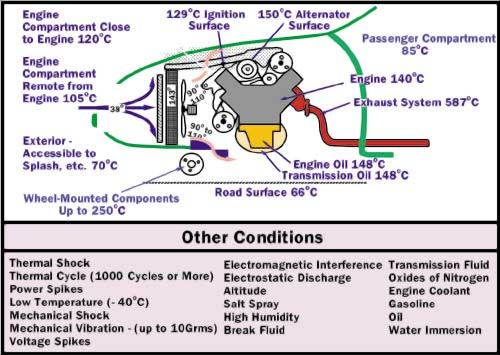
\includegraphics[width=.8\textwidth]{Chapter1/Figs/automotive_cond.png}
	\caption{Stringent automotive conditions presented by the Automotive Electronics Council~\cite{1393072,ISO16750}}
	\label{fig:automotive-cond}
\end{figure}

Aiming a Smart Vehicle, the sensor market is arguably the most important one. The vehicle smartness is given by strong processing unit which could not stand the harsh environment in which most of the sensors should sustain. To transfer the information of sensors to those processing units, it is mandatory to place the Analog-to-Digital converters (ADC) as close as possible to the sensor with a sampling rate sufficiently high for the future application of autonomous car. For all these reasons, ADC design is a challenge since it should remain reliable even under performance variation \cite{Cai2012}.

%********************************** %First Section  **************************************
\section{Motivation}   % section 1.1
To that extent, a low-cost, fast and accurate ADC operating in those harsh conditions is a good ally for equipment manufacturers. To decrease the cost, the area is a major concern. Considering re-use of the ADC as an IP-bloc, the area should be limited to less than half a square millimeter.
In the automotive environment, ADCs are the usual interface with environmental sensors and motor control sensors.

\begin{table}[htp]
	\centering
	\caption{Specification of target ADC}
	\label{tbl:adc-spec}
	\rowcolors{2}{gray!15}{white}
	\begin{tabular}{ll}
		\toprule
		& Criterion                                                                                                                                                   \\ \midrule
		Operating Temperature            & -40 $\degree$ C -- +175 $\degree$ C                                                                                               \\
		Supply Voltage                   & 1.8 V $\pm$ 10 \%                                                                                                                              \\
		Differential Input Voltage Range & $\pm$ 1V                                                                                                                                       \\
		Area                             & \textless 0.5 \(\rm mm^2\)                                                                                                                                      \\
		Conversion Speed                 & 20 MSamples/s                                                                                                                                               \\
		Maximum Clock Frequency          & 100 MHz\\
		Clock Duty-Cycle                 & 40 -- 60 \%                                                                                                                                                 \\
		Latency                          & 500 ns                                                                                                                                                      \\
		Resolution                       & $\geq$ 12-bits                                                                                          \\
		\rowcolor{white}\multirow{-1}{*}{SNDR }   & min 74 dB for $F_s$ \textless 5 MHz\\
		\rowcolor{white}                      & min 68 dB for 5 MHz \textless $F_s$  \textless 10 MHz,\\
		\rowcolor{white}						& min 62 dB for $F_s$  \textgreater 10 MHz  \\
		SFDR (Full-Scale)                & min 68 dB                                                                                               \\
		DNL                              & \textless LSB/2                                                                                       \\
		INL                              & \textless LSB/2 best-fit method                                                                                    \\
		Offset Error                     & \textless 4 LSB                                                                                                                                             \\
		Gain Error                       & \textless 4 LSB                                                                                                                                             \\
		Adjacent ADC mismatch Error      & \textless 4 LSB                                                                                                                                             \\
		Energy, $E_s = P/F_s$            & 0.75 nJ/sample      \\ \bottomrule
	\end{tabular}
\end{table}

\nomenclature[z]{PVT}{Process-Voltage-Temperature}
The frequency spectrum of such application being limited, the ADC does not need to tackle for Gigahertz sampling. The accuracy and the linearity are of much importance. Nevertheless, the vehicle communicates the sensors' information. The bandwidth of the communication signals is few megahertz.
To fulfill the need, the minimum requirements for a final product are listed in Table~\ref{tbl:adc-spec}. The order of importance is the area, the resolution, the power consumption, and the conversion speed. It is important to highlight the temperature range and the ratio between the conversion speed and the maximum clock frequency equal to 5. This ratio also called Oversampling Ratio (OSR) is the number of clock cycle allowed to perform a conversion.

To respond to the future need of the automotive environment, we aim to design an ADC over a wide temperature range from -40\(\degree \)C to 175\(\degree \)C with the following characteristics:

\begin{itemize}
	\item A maximum oversampling ratio of 5
	\item SNDR greater than 68 dB
	\item a consumption of less than 0.75 nJ/sample
	\item and target a silicon area less than 0.5 \(\rm mm^2 \) for cost reason
\end{itemize}

with a preference sets on the minimization of the silicon area, before the minimization of the power consumption, the resolution, and the speed.

The XT018 technology, from the XFAB Silicon Foundries, is ideal for system-on-chip (SoC) applications in the automotive market such as control devices inside combustion engine compartments or electric engine housings with temperature range up to 175$\degree$C, as well as robust medical applications which should sustain high voltages~\cite{XT018XFab}. Such technology is a SOI process, which uses a deep-trench buried oxide that leads to a very low junction leakage current even at high temperatures.

\section{Thesis Organization}

This work focuses on the design of high-precision, high-speed and energy efficient ADC under the harsh environment the automotive one represents. A emphasis is on doing such design in an SOI CMOS process under stringent Process-Voltage-Temperature (PVT) variations. Our main contribution relies on the development of a new hybrid topology proposal using 3 stages to cope with such constraints based on a top-down approach: a counting stage inherently linear, an algorithmic stage to increase rapidly the precision, and a SAR stage for area and power consumption trade-off.

We review the operation of conventional ADC topologies in Chapter~\ref{sec:soa}. Their advantages and source of errors are discussed to present why some architectures are predominant in high-temperature conditions. Namely, few of them such as \(\Delta \Sigma\), SAR, and pipelined are able to cope with analog imperfections coming from the temperature. The proposed architecture is then presented to benefit from the strength of each one.

Section~\ref{sec:temperature-analogue} then discusses the challenge of analog design over a large temperature range from -40\(\degree\)C to +175\(\degree\)C. Phenomena tightly linked to the temperature are analyzed to highlight the design trade-offs when considering temperature effects. Based on a \(g_m/I_D\) methodology, the insight gained from this analysis is then reused during the design phase.

Having the severe degradation, we discuss the enhancement ported to our topology proposal to glean the maximum of performances within the smallest footprint in a 180 nm technology. Alongside the optimization, Chapter~\ref{sec:adc-implementation} considers the reliability and introduces the case of pseudo-asynchronous design to relax timing restrictions in the digital part over temperature. We have defined a methodology for the design and characterization of such converter by using a testbench comparing a high-level model of the converter, defined in Verilog-AMS, and a schematic description of the converter, able to use macromodels of the components or their transistor-level description. A MATLAB post-processing can extract the main characteristics such as the accuracy, the DNL, the INL ...

The design of mandatory analog blocks, which are respectively comparators and operational amplifier, is examined to ensure the expected behavior for a rigorous 6\(\sigma\) process variation. To achieve this, a new time delay model has been developed for the Double Tail comparator. This model has been presented during the ECCTD conference held in 2017. Meanwhile, the layout consideration to get the most of the op-amp is also discussed in Chapter~\ref{sec:analog-building-bloc}.

Despite the fact the ADC test chip is in a finalization stage, experimentation is key in the validation process of IP components. Details in the realization of test chips in temperature which are worth to be discussed are presented in Chapter~\ref{sec:tests-meas}. With a chip dedicated to the assessment of comparators, their offset, the delay, the noise, and the hysteresis measurement circuits are implemented. The delay of high speed clocked comparator has been measured with a new measurement circuit presented during the ECCTD in 2017. After the enhancement of our topology proposal, only the testability of the last stage has seen its complexity increased. A second test chip assesses the effectiveness of pseudo-asynchronous design at high temperature and extracts static metrics of the last stage (DNL, INL, ...). Then, the last section focuses on the ADC test chip. Its design and preliminary results of the ADC are presented. Chapter~\ref{sec:perspectives} concludes our research findings and suggests potential future work.
  % Intro & Motivation
%!TEX root = ../thesis.tex
% chktex-file 1
% chktex-file 24
%*******************************************************************************
%****************************** Second Chapter *********************************
%*******************************************************************************

\chapter{State of the Art}
\label{sec:soa}
% **************************** Define Graphics Path **************************
\ifpdf
    \graphicspath{{Chapter2/Figs/Raster/}{Chapter2/Figs/PDF/}{Chapter2/Figs/}}
\else
    \graphicspath{{Chapter2/Figs/Vector/}{Chapter2/Figs/}}
\fi
\nomenclature[z]{ADC}{Analog-to-Digital Converters}
The performance of an ADC can be defined by the fidelity of signal representation and the bandwidth of the signal which can be represented. In other terms, the key criteria of an ADC are the Signal to Noise and Distortion Ratio (SNDR) and the Nyquist frequency ($F_{\rm snyq}$). \figurename~\ref{fig:topology-sndr-fsnyq-comparison} distinguishes ADC families using both criteria. These ADC families are:
\begin{enumerate}
	\item Flash, having a higher time-efficiency but too expensive for high resolution as power consumption and the area scales with resolution;
	\item $\Delta\Sigma$, being the best trade-off between resolution and speed but power consumption and area scales with requirements;
	\item Pipelined and Algorithmic, being high-speed and high-resolution but power consumption and area hungry;
	\item SAR, performing either high-resolution or high-speed conversions for a very low power consumption.
\end{enumerate}

\begin{figure}[htp]
	\centering
	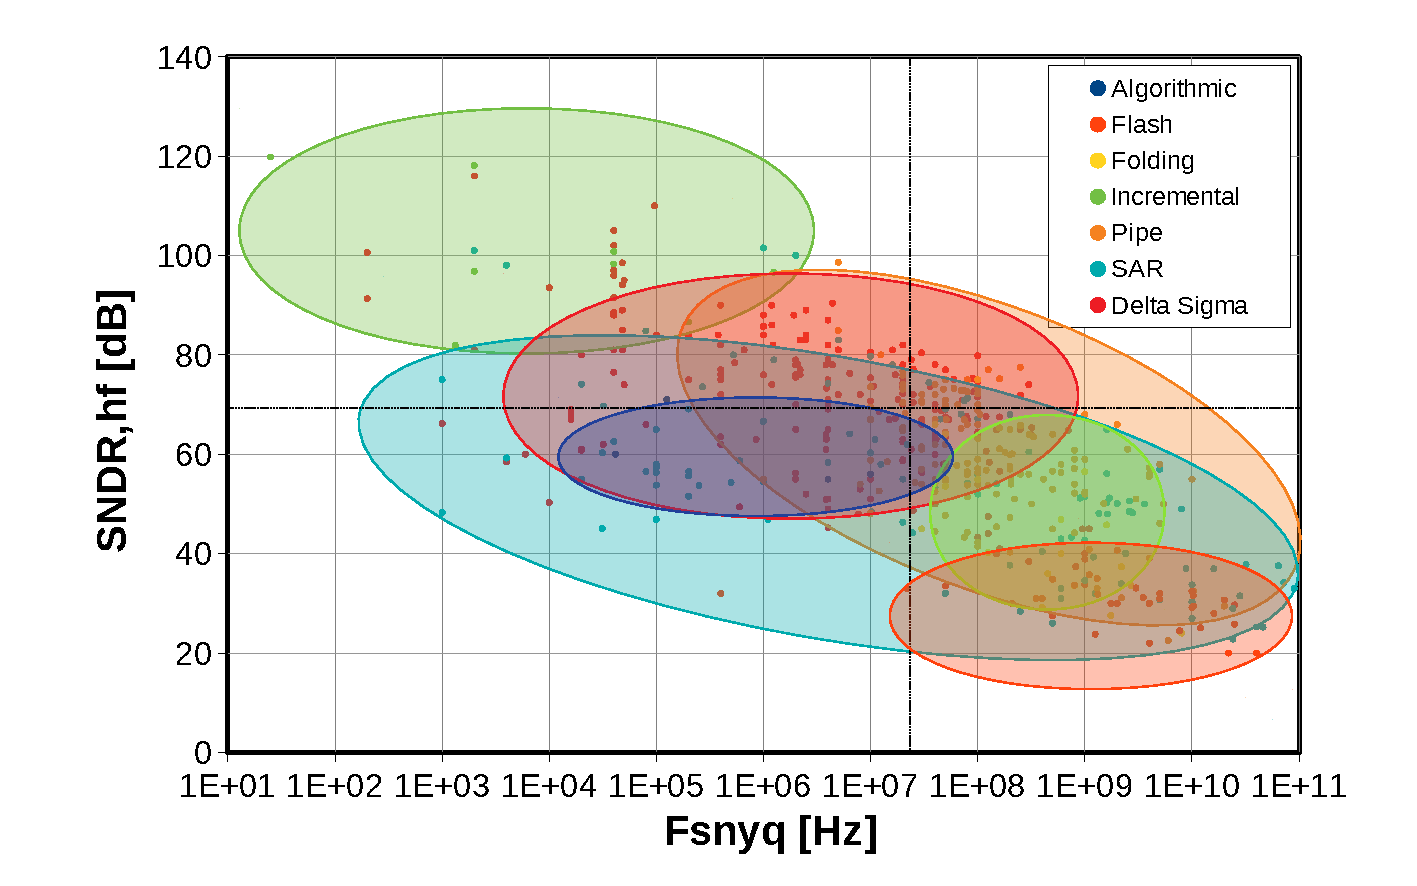
\includegraphics[width=.8\textwidth]{Chapter2/Figs/Vector/sndr_fsnyq_topology.pdf}
	\caption{Comparison of ADC topology in the SNDR-$F_{\rm snyq}$ space based on publication in ISSCC and VLSI from 1997 to 2018~\cite{MurmannSurvey}}
	\label{fig:topology-sndr-fsnyq-comparison}
\end{figure}
An analysis of the chart allows the designer to properly decide what kind of a converter topology is desired according to the speed and the signal fidelity required. For instance, Flash ADCs achieve rather low SNDR at very high speed while Incremental ADCs achieve high fidelity signal representation for low signal bandwidth.

It is worth to mention that Folding ADCs are close to the ADC specification in this thesis. Besides that, prior art topologies are often requiring more than 5 clock cycles per conversion to reach the resolution expected. In this scenario, there is no immediate solution to propose a topology that meets the specification requirements. That's why a new topology is proposed in this work. This chapter begins with an analysis of classical ADC architectures. A large emphasis is set on the low-OSR and high-resolution possibility at a medium conversion rate.

Later in this chapter, a brief review of ADC design over extended temperature range is presented. At high temperatures, transistors suffer from several defects that degrade their performances which impacts system performance. The impact of the temperature at the device level and the material dependences are studied using CMOS XT018 technology. \nomenclature[z]{CMOS}{Complementary Metal-Oxide-Semiconductor}

\section{Analog-to-Digital Converters}
\subsection{Flash}                             % section 2.1
\label{sec:flash-adc}
Flash ADCs proceed a conversion by comparing the analog input voltage with several reference voltages. While a resistive divider generates references, the comparators provide in the same clock cycle the comparison results of the input voltage with each reference voltage, as represented in \figurename~\ref{fig:flash_kickback}.

\begin{figure}[htp]
	\centering
	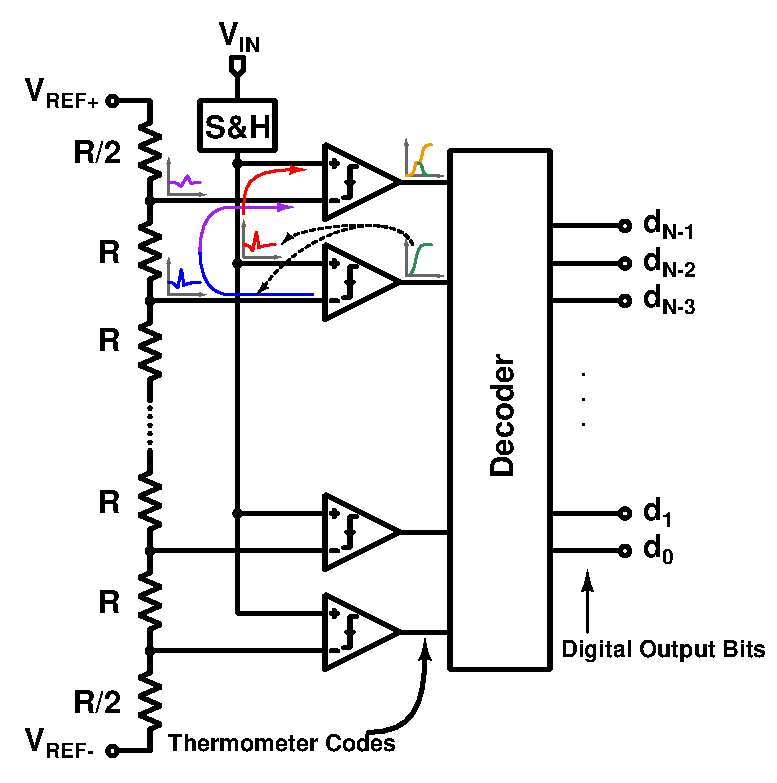
\includegraphics[height=6cm]{Chapter3/Figs/flash_adc.ps}
	\caption{Flash ADC architecture: illustration of comparators' kickback noise impacts other comparators through the reference ladder}
	\label{fig:flash_kickback}
\end{figure}

Thus, an analog input below the \(i^{th} \) reference voltage produces an output of \(i-1 \) ones followed by zeros. A rising input voltage increasing the number of consecutive ones at the output, this architecture is known as thermometer code encoding. For an N-bit converter, a Flash ADC requires \(2^N-1\) comparators, and a decoder usually follows to bring an N-bit binary word. The time-efficiency of this architecture is too expensive for high-resolution ADC, as both the power consumption and the area scales with the desired resolution. In addition to that, the clock skew has an important impact on the output code. The decision of a comparator disturbs the decision of another one deciding later. \figurename~\ref{fig:flash_kickback} illustrates the kickback noise generated source of bubble codes (zero(s) trapped in the ones of thermometer codes). Usually Flash does not exceed 8-bits.

A different kind of Flash ADC, able to achieve 8-bits or more, is the Folding ADC. In Folding ADCs, a pre-estimation is performed by a Flash ADC. Then, a folding amplifier folds the signal according to the conversion results of the first Flash ADC. For a ramp input, it generates a sawtooth waveform corresponding to the error of conversion of the "first stage" as depicted by \figurename~\ref{fig:folding_principle}. Thus, it generates the Most-Significant-Bits (MSB).

\begin{figure}[htp]
	\centering
	\resizebox{0.8\textwidth}{!} {\def\putbox#1#2#3#4{\makebox[0in][l]{\makebox[#1][l]{}\raisebox{\baselineskip}[0in][0in]{\raisebox{#2}[0in][0in]{\scalebox{#3}{#4}}}}}
\def\rightbox#1{\makebox[0in][r]{#1}}
\def\centbox#1{\makebox[0in]{#1}}
\def\topbox#1{\raisebox{-0.60\baselineskip}[0in][0in]{#1}}
\def\midbox#1{\raisebox{-0.20\baselineskip}[0in][0in]{#1}}
   \scalebox{1}{
   \normalsize
   \parbox{5.90104in}{
   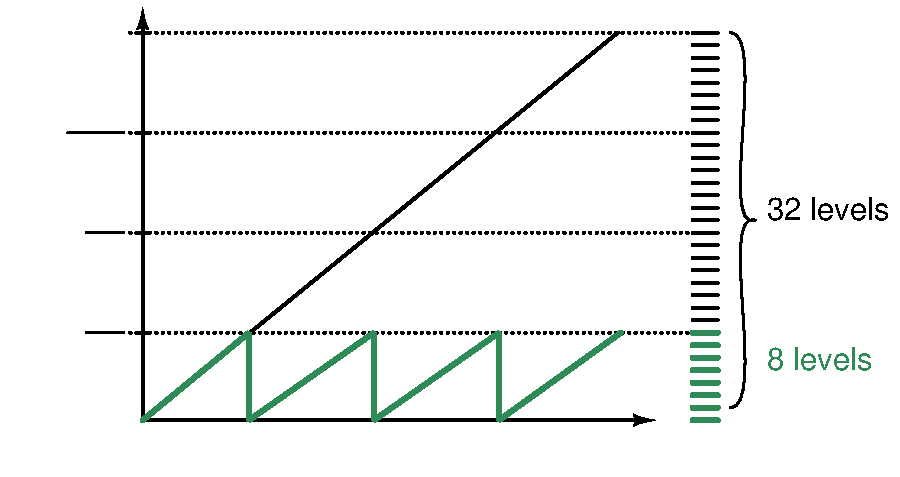
\includegraphics[scale=1]{Chapter3/Figs/folding_signal_principle}\\
   % translate x=364 y=254 scale 0.38
   \putbox{1.70in}{0.09in}{1.20}{Input Voltage [V]}%
   \putbox{0.20in}{0.67in}{1.20}{\rotatebox{-270}{Voltage Processed [V]}}%
   \putbox{0.54in}{1.71in}{0.84}{\(V_{REF}\)}%
   \putbox{0.41in}{2.38in}{0.84}{3}%
   \putbox{0.66in}{1.50in}{0.84}{2}%
   \putbox{0.54in}{1.05in}{0.84}{\(V_{REF}\)}%
   \putbox{0.54in}{2.38in}{0.84}{\(V_{REF}\)}%
   \putbox{0.54in}{2.96in}{0.84}{\(V_{REF}\)}%
   \putbox{0.66in}{0.84in}{0.84}{4}%
   \putbox{0.58in}{2.17in}{0.84}{4}%
   } % close 'parbox'
   } % close 'scalebox'
   \vspace{-\baselineskip} % this is not necessary, but looks better
}
	\caption{Signal folding principle to reduce the number of needed comparators in a 5-bits ADC example}
	\label{fig:folding_principle}
\end{figure}

In the same time, a second Flash ADC performs the conversion of the folded signal. This reduces the total number of components relaxing previous constraints of a first Flash ADC~\cite{VanDePlassche1979, Grift1987, Nauta1995, Vorenkamp1997} to save area and power consumption. Unfortunately, the Folding topology should have a linearity greater than the LSB's Flash ADC. Such linearity issues can be corrected either by a digital calibration or by a resistive interpolation~\cite{Vorenkamp1997}. Such topology of ADC allows the cascade of several stages~\cite{Taft2009, Buck2017}, making it a good candidate to achieve medium resolution at high speed~\cite{Vorenkamp1997, Pan2000}. The biggest flaws of Folding Flash ADCs are the area and the power consumption despite works to reduce them~\cite{Costa2013}. The comparison table~\ref{table:folding_comparison_table} reveals the resolution of such architectures of Flash ADC\@. They achieve a very high speed with a small latency. This can be viewed as a trade-off between time and resolution.
\begin{table}[htp]
	\caption{Folding ADC in the literature}
	\centering
	\label{table:folding_comparison_table}
	\begin{tabular}{L{3.5\charwidth} C{23\charwidth} R{6.5\charwidth} R{4\charwidth} S[table-format=2.2, table-column-width=5.2\charwidth] R{6\charwidth} R{5.5\charwidth} R{3.5\charwidth}}
		\toprule
		Ref. & Architecture & Techno. [nm] & \(F_{snyq}\) [MHz] & {\makecell{{Area}\\{[\(mm^2 \)]}}} & Supply [V] & Power [mW] & Res. \tabularnewline \midrule
		\cite{Vorenkamp1997} & Folding \& Interpolation  & 1000 &   60 &    7 &   5 &  300 & 12 \\
		\cite{Taft2009}      & Cascaded Folding          &  180 & 1000 &   49 & 1.8 & 1260 & 10 \\
		\cite{Buck2017}      & Folding \& Interpolation  &  250 & 6000 & 13.3 & 5.1/3 & 10200 & 10 \\
		\cite{Costa2013}     & switched-cap Folding      &  350 &  100 &   NA & 3.3 &  2.5 &  8 \\
		\cite{Choe2001}      & Folding                   &  500 &  100 & 1.68 &   5 &  165 &  8 \\
		\bottomrule
	\end{tabular}
\end{table}
\nomenclature[A-Fsnyq]{$F_{snyq}$}{nyquist frequency}


\subsection{\(\Delta\Sigma \) Converters}      % section 2.3
\label{sec:sd-isd-adc}
\subsubsection{\(\Delta\Sigma \) Modulation}
Delta-Sigma (\(\Delta\Sigma \)) modulation efficiently performs high-resolution data conversion using oversampling. For the sake of clarity, let's us consider first a sine wave converted by an ADC without oversampling. The power spectral density, \figurename~\ref{fig:spectrum-sine-nyquist}, is made of a tone representing the signal power, a floor corresponding to the quantization noise, and other sources of noise. The effective number of bits (ENOB) is related to the gap between the noise floor and the signal level. The bigger the gap is, the higher is the ENOB of the converter.

\begin{figure}[htp]
	\centering
	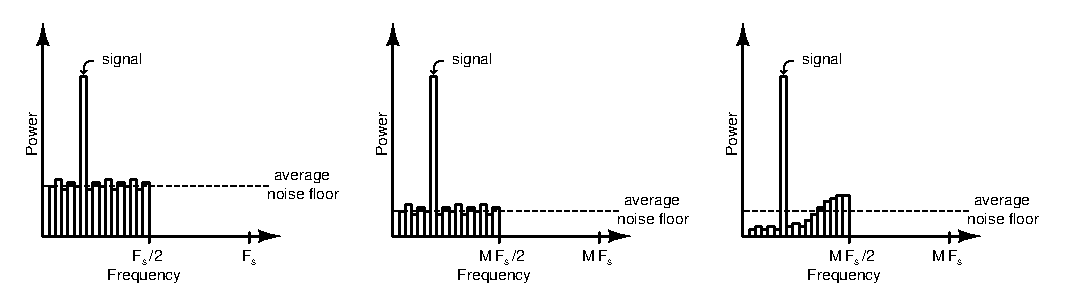
\includegraphics[width=\textwidth]{Chapter2/Figs/Vector/sd-noise-shaping.ps}
	\begin{subfigure}[b]{0.33\textwidth}
		\subcaption{Signal Spectrum}
		\label{fig:spectrum-sine-nyquist}
	\end{subfigure}
	\begin{subfigure}[b]{0.33\textwidth}
		\subcaption{Oversampling by M}
		\label{fig:spectrum-sine-oversampling}
	\end{subfigure}
	\begin{subfigure}[b]{0.33\textwidth}
		\subcaption{Noise Shaping}
	\end{subfigure}
	\caption{Principle of the $\Delta \Sigma$ ADC to perform a high-resolution conversion}
	\label{}
\end{figure}

By increasing the sampling frequency $F_s$ by a factor $M$, the quantization noise decreases by $M$; it is now spread over a wider frequency range ($F_s \cdot M$). The integral of the noise over the frequency band of interest remains constant as illustrated from \figurename~\ref{fig:spectrum-sine-nyquist} to \figurename~\ref{fig:spectrum-sine-oversampling}. By filtering the spectrum with a cut off frequency of $F_S/2$, the noise power reduced in the signal bandwidth. To enhance further performance, the distribution of the noise can be shaped to push the noise at higher frequencies than the cut-off of the digital filter.

\begin{figure}[htp]
	\centering
	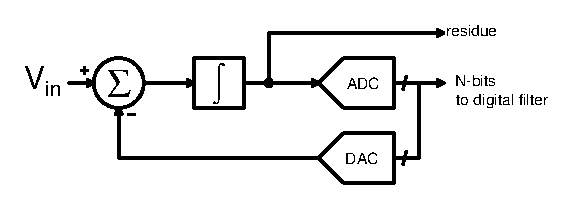
\includegraphics[width=0.75\textwidth]{Chapter2/Figs/Vector/sigma-delta.ps}
	\caption{Multi-bits $\Delta\Sigma$ converter}
	\label{fig:multi-bit}
\end{figure}

To convert the input signal, a $\Delta\Sigma$ modulator is similar to a regulation loop in which the integrator controller monitors the process of conversion as illustrated in \figurename~\ref{fig:multi-bit}. The integral term permits the rejection of a step disturbance and ensures that for a stepped input, the static error of the conversion process is nulled. With respect to the input signal, the integrator behaves like a low-pass filter. To the contrary, for the quantification noise coming from the feedback path, the integrator is likewise a high-pass filter. The noise is shaped. In consequence, there is a signal transfer function (STF) and a noise transfer function (NTF). The implementation imperfections, including matching errors and offsets which limit the obtainable resolution of Nyquist rate converters, can thus be surmounted as these are in the feedback path. Furthermore, the oversampling reduces the constraint of the anti-aliasing filter in front of ADC by relaxing the filter order required.\nomenclature[z]{OSR}{Oversampling Ratio}

To increase the sampling rate, it is necessary to reduce the oversampling ratio (OSR). To preserve the resolution, the noise-shaping filter order should be increased. The improvement originates from the extra integrator in the forward path. Unfortunately, the feedback structure of the modulator is prone to instability for high-order of noise shaping ($\geq$ 3). Besides, high-order modulators suffer from a stability dependency on system parameters such as integrator gains and delays, input amplitude, transients, initial conditions, or even saturation limit cycles~\cite{Hein1993,Baird1994,Steven1996}. For modulator stability, the integrator signal shall be weighted appropriately. Reducing the input amplitude is another way to stabilize the system, as well as reducing the error signal integrated to prevent saturation of the following integrator. In this regard, multi-bit quantization limits the excursion of the integrator. However, the implementation of the multi-level error feedback DACs can significantly reduce the modulator performance if the DAC is not extremely linear~\cite{Medeiro1999}.


\subsubsection{Incremental-\(\Delta\Sigma \)}
\label{sec:soa-isd}
Unlike conventional \(\Delta\Sigma \) ADCs, the analog loop filter and the digital filter in Incremental-\(\Delta\Sigma \) (\(I\Delta\Sigma \)) ADCs are reset after oversampling each input sample. As a result, \(I\Delta\Sigma \) ADC can offer sample-by-sample conversion much like Nyquist-rate ADC allowing multiplexing of different inputs to be done without crosstalk.

\begin{figure}[htp]
	\centering
	\resizebox{\textwidth}{!} {\def\putbox#1#2#3#4{\makebox[0in][l]{\makebox[#1][l]{}\raisebox{\baselineskip}[0in][0in]{\raisebox{#2}[0in][0in]{\scalebox{#3}{#4}}}}}
\def\rightbox#1{\makebox[0in][r]{#1}}
\def\centbox#1{\makebox[0in]{#1}}
\def\topbox#1{\raisebox{-0.60\baselineskip}[0in][0in]{#1}}
\def\midbox#1{\raisebox{-0.20\baselineskip}[0in][0in]{#1}}
   \scalebox{1}{
   \normalsize
   \parbox{7.08333in}{
   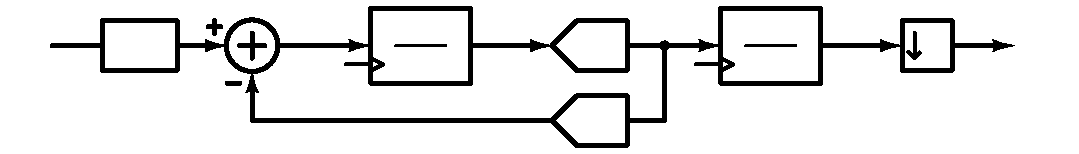
\includegraphics[scale=1]{Chapter3/Figs/isd_first_order_principle}\\
   % translate x=568 y=192 scale 0.38
   \putbox{0.81in}{0.68in}{0.90}{S/H}%
   \putbox{2.14in}{0.56in}{0.90}{$\Phi_r$}%
   \putbox{2.76in}{0.76in}{0.96}{1}%
   \putbox{2.68in}{0.56in}{0.96}{Z-1}%
   \putbox{3.85in}{0.68in}{0.90}{A/D}%
   \putbox{3.85in}{0.18in}{0.90}{D/A}%
   \putbox{4.47in}{0.56in}{0.90}{$\Phi_r$}%
   \putbox{5.10in}{0.76in}{0.96}{1}%
   \putbox{5.01in}{0.56in}{0.96}{Z-1}%
   \putbox{4.35in}{0.85in}{1.20}{$d_k$}%
   \putbox{0.06in}{0.68in}{1.20}{$V_{in}$}%
   \putbox{6.81in}{0.68in}{1.20}{$D_{out}$}%
   \putbox{6.18in}{0.68in}{0.90}{M}%
   } % close 'parbox'
   } % close 'scalebox'
   \vspace{-\baselineskip} % this is not necessary, but looks better
}
	\caption{First Order Incremental-\(\Delta\Sigma \)}
	\label{fig:isd_first_order_principle}
\end{figure}

A first order \(I\Delta\Sigma \) as represented in \figurename~\ref{fig:isd_first_order_principle} has a resolution of N-bits is achieved in \(2^N \) clock cycle. Different approaches have been proposed to significantly enhance the conversion speed and/or resolution of \(I\Delta\Sigma \) ADC~\cite{Markus2004,Quiquempoix2006,Caldwell2010}. The most popular alternatives are high-order architectures~\cite{Au1997,Babanezhad1991,Baird1996}. Recent advances in \(I\Delta\Sigma \) ADC showcase further improvement in power efficiency by employing inverter-based integrators~\cite{Chae2009}, or comparator based integrators~\cite{Yamamoto2012}.

An added benefit to \(I\Delta\Sigma \) is the simplicity of the decimation filter. As the output of the regulation loop is the bits of the conversion process, these represent the input signal. So, the error at the input of the integrator is in the best case zero. The output of the controller keeping the error null, the digital reconstruction filter should have the same transfer function as the controller to represent the input. For a first-order modulator, the input signal is reconstituted by counting output bits, while for higher order the representation of the input signal is given by a weighted multiple integral. For a third order modulator, \(V_{\rm in}\) is thus estimated by the equation~(\ref{eqn:isd-decimation}).

\begin{equation}
	\frac{V_{\rm in}}{V_{\rm ref}}\approx \frac{3!}{(n-2)(n-1)n}\sum_{m=0}^{n-1}\sum_{l=0}^{m-1}\sum_{k=0}^{l-1}d_{k}
\label{eqn:isd-decimation}
\end{equation}

% In~\cite{Caldwell2010} the number of output level for an \(L^{th}\)-order converter with \(N\) quantizer levels and an OSR of \(M\) is
% \begin{equation}
% 	\alpha(N-1)\frac{(M+L-1)!}{L!(M-1)!}+1
% \label{eqn:isd-levels}
% \end{equation}

% The coefficient \(\alpha \) is the maximum converter amplitude that keeps the quantizer input bounded and is usually less than unity. The Signal-to-Noise Ratio (SNR) is thus defined as \(SNR = 6.02N + 1.76dB\).
In other terms, the input-referred noise of an Incremental-\(\Delta\Sigma \) comes from a weight association of each output bits of the quantizer, and for higher order modulators past bits have a higher weighting than future ones because the digital filter has non-uniform weighting coefficients for higher order modulators. The equation~(\ref{eqn:isd_noise}) expresses the total input-referred noise power \(\overline{v_{n}^{2}}\)
\nomenclature[z]{SNR}{Signal over Noise Ratio}
\begin{equation}
	\overline{v_{n}^{2}}=\sum_{i=1}^{M}w_{i}^{2}\overline{v_{s}^{2}}=\overline{v_{s}^{2}}\sum_{i=1}^{M}w_{i}^{2}
\label{eqn:isd_noise}
\end{equation}
where \(\overline{v_{s}^{2}}\) is the input noise power of each sample, \(M\) is the OSR, and \(w_i\) is the weight associated with each quantization.
\nomenclature[C-comp]{$\overline{X}$}{complementary of signal X}

A first order Incremental-\(\Delta \Sigma\) of N-bits, which is achieved in M clock cycles per sample, averages M-times the input and the quantization noise error introduced by the quantizer. The weight of each quantization is thus \(w_i=1/M\). The resulting input-referred noise power is \(\overline{v_{n}^{2}}/M\), as expected for an ADC oversampled by M. Nevertheless, the first clock cycle is dedicated to the reset of the integrator, which limits the resolution in low-OSR architecture.

\subsubsection{MASH}
To the opposite of high-order modulator, first-order modulators are inherently stable without weighting the output of the integrator. A cascade of such modulators results in an increased noise shaping order without the stability issue or sacrificing the input amplitude~\cite{Brooks1997}. Also called Multi-stAge noise-SHaping (MASH), they have the advantage that no individual modulator needs to be designed with a high-order filter; the total filter order can be spread out across many different stages so that each individual \(\Delta\Sigma \) stage will only be of low order. The modulator stability will be a function of the individual lower order modulators rather than the total order of the modulator.

\begin{figure}[htp]
    \centering
    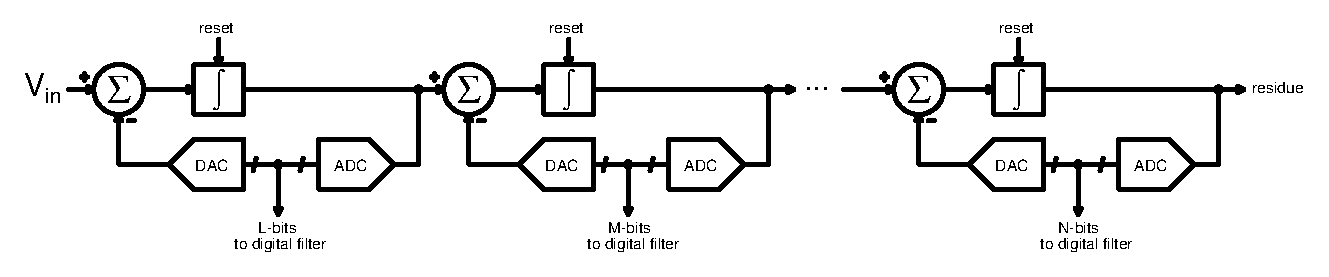
\includegraphics[width=\textwidth]{Chapter2/Figs/Vector/sigma-delta-mash.ps}
    \caption{1-1-...-1 MASH $\Delta\Sigma$ converter}
    \label{fig:multi-bit}
\end{figure}

The digital output of individual \(\Delta\Sigma \) modulators is then processed by a digital filter. It is designed to reduce error introduced in first stages by the product of the Noise-Transfer-Function of each stage. This cancellation is dependent on matching between the digital filters and the analog filters within modulators. The latter is one of the major limitations for high-resolution cascaded \(\Delta\Sigma \) modulators leveraged by digital calibration~\cite{Cauwenberghs2000}.

\subsubsection{Mixed Architecture based on $\Delta\Sigma$}
Other alternatives are the extended counting (EC-ADC)~\cite{Jeon2017,Baird1995,Chen2016} and the extended range (ER-ADC)~\cite{Agah2010,Rossi2009} architectures, which combine the \(I\Delta\Sigma \) ADC with a low-power Nyquist-rate ADC\@. The main difference between the two is that in an EC-ADC, the \(I\Delta\Sigma \) ADC hardware is usually reused and reconfigured as a cyclic ADC, while in an ER-ADC, the residue of the \(I\Delta\Sigma \) is processed by another Nyquist-rate ADC\@.

The table~\ref{table:sigma_delta_comparison_table} compares \(I\Delta\Sigma \) to MASH and mixed architecture to highlight the main characteristics of these converters.

\begin{table}[htp]
	\caption{\(I\Delta\Sigma \)-ADC in the literature}
	\centering
	\label{table:sigma_delta_comparison_table}
	\begin{tabular}{L{3.5\charwidth} R{16.5\charwidth} R{6\charwidth} C{5\charwidth} R{4\charwidth} S[table-format=2.2, table-column-width=6\charwidth] R{6\charwidth} S[table-format=2.2, table-column-width=6\charwidth] C{3.5\charwidth}}
	\toprule
	Ref. & Architecture & Techno. [nm] & \(F_{snyq}\) [kHz] & OSR & {\makecell{{Area}\\{[\(mm^2 \)]}}} & Supply [V] & {\makecell{{Power}\\{[mW]}}} & Res. \\
	\midrule
	\cite{Quiquempoix2006} & \(3^{rd}\) Order \(I\Delta\Sigma \) & 600 & 30.72 & 512 & 2.08 & 2.5/5 & 0.6 & 22 \\
	\cite{Chae2009} & \(3^{rd}\) Order \(\Delta\Sigma \) & 180 & 40 & 100 & 0.715 & 0.7 & 0.036 & 14 \\
	\cite{Jeon2017} & EC-\(\Delta\Sigma \) & 180 & 185 & 8 & 0.0069 & 1.8 & 0.022 & 12 \\
	\cite{Agah2010} & ER-\(I\Delta\Sigma \) & 180 & 1000 & 45 & 3.5 & 1.8 & 38.1 & 14 \\
	\cite{Liu2017} & 1-1-1~MASH CT-\(\Delta\Sigma \) & 40 & 50000 & 29.7 & 0.177 & 1.2/2.5 & 19.7 & 11 \\
	\bottomrule
	\end{tabular}
\end{table}

\subsection{Pipelined and Algorithmic}               % section 2.4
\label{sec:pipe-adc}
Pipelined and Algorithmic converters are fundamentally similar. They are based on a common build bloc: the analog processor. This bloc is made of an ADC-DAC chain to estimate the input, whose difference with it is then multiplied by an arbitrary factor A. The output of the analog processor is the conversion residue amplified. A is the radix of conversion and it is often set to 2. Represented in \figurename~\ref{fig:pipelined-principle}, pipelined ADCs are a cascade of these extracting N-bits for each clock cycle. The algorithmic depicted in \figurename~\ref{fig:algorithmic-principle}, reuses the analog processor over and over by recycling the residue. After M clock cycle, both architectures extract $N\times M$ bits with the same latency. However, for the same clock frequency and the number of bits extracted, a pipelined of M-stages has a sampling frequency M-times higher than an algorithmic with M-clock cycles. In addition to that, pipelined ADCs occupy a bigger area than algorithmic.

\begin{figure}[htp]
	\centering
    \begin{subfigure}[b]{\textwidth}
        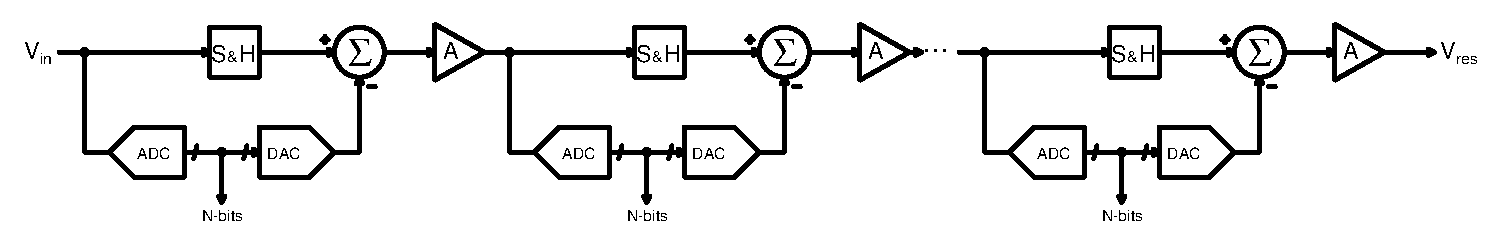
\includegraphics[width=\textwidth]{Chapter2/Figs/Vector/pipelined.ps}
        \subcaption{Pipelined}
        \label{fig:pipelined-principle}
	\end{subfigure}
	\begin{subfigure}[b]{0.4\textwidth}
        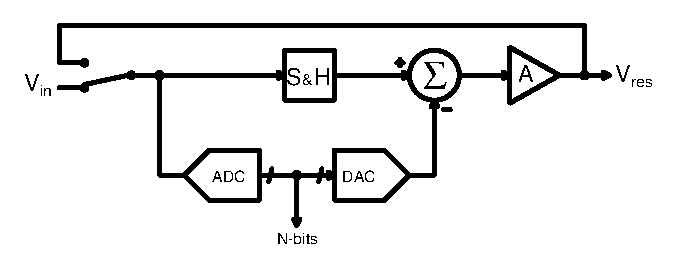
\includegraphics[width=\textwidth]{Chapter2/Figs/Vector/algorithmic.ps}
        \subcaption{Algorithmic}
        \label{fig:algorithmic-principle}
    \end{subfigure}
	\caption{Principle of the pipelined and of the algorithmic converter}
	\label{fig:algo_desc}
\end{figure}

These architectures have garnered much attention recently due to their low-voltage and higher integration characteristics~\cite{Steyaert2012,Lee2011,SKLee2011,Brooks2009,Hershberg2012,YLim2015,YLim2015FD,Megawer2016,YCao2017}. Systems that inherently require a low-voltage operation, such as biomedical and wireless sensor applications, also motivate research in this area and demonstrate their versatility~\cite{Steyaert2012,Lee2011,SKLee2011}.

% For a gain \(A=2\), the algorithmic ADC performs a modified binary search algorithm to digitize the input voltage. In this regard, the conversion is similar to SAR ADC with the fact that it provides the error of conversion\@.

Current mode method offers an ease of implementation of basic functions such as summation and scaling, and they are also appropriate for low voltage application. Some current mode algorithmic have been designed recently~\cite{Nairn1990,Wang1991,Khodabndehloo2009,Bhatia2011}. Even if current mode design requires lower voltage swing and increase noise immunity, the accuracy is limited by current mirror matching. This can be improved by increasing transistor sizes and biasing currents. Larger transistor sizes and larger reference current, however, need larger chip area and higher power consumption. This trend establishes a trade-off which may turn the proposed Current Mode ADC in a less attractive solution than other ADCs\cite{Wang1991}.

\begin{figure}[htp]
	\centering
    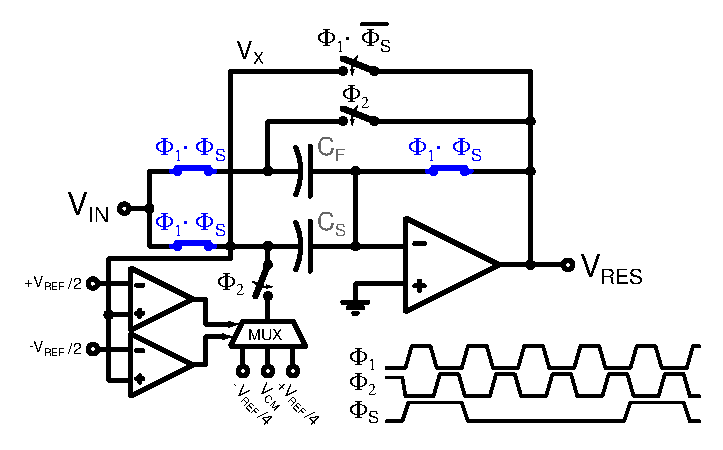
\includegraphics[width=0.7\textwidth]{Chapter3/Figs/algo_mdac_std.ps}
	\caption{Principle of a 3-levels Flip-Around MDAC in the realization of an Algorithmic converter}
	\label{fig:algo_mdac}
\end{figure}

A common implementation of the algorithmic converter is by building the stage around a Flip-Around Multiplying DAC (FA-MDAC). This way, the closed-loop gain is defined by a ratio of capacitors whose mismatch is well controlled, as represented in \figurename~\ref{fig:algo_mdac}. A simple differential pair is a valid amplifier to operate under low-supply condition. As the resolution increases (recycling of its inner self-error), the gain of the amplifier shall drastically increase. By stacking transistors the output swing is thus limited, and non-linearity occurs. Therefore, medium to high-resolution algorithmic ADCs require a digital compensation~\cite{Murmann2003} or an adjustment of its residue curve~\cite{Inoue2017,Naderi2017}.\nomenclature[z]{MDAC}{Multiplying Digital-to-Analog Converter}

The amplifier or Operational Transconductance Amplifier (OTA) is power hungry. Few analog circuits exist to emulate them with a reduced power consumption such as the comparator based MDAC and the ring amplifier based MDAC. The table~\ref{table:algo_comparison_table} highlights the main characteristics of the algorithmic converters. \nomenclature[z]{OTA}{Operational Transconductance Amplifier}
\begin{table}[htp]
	\caption{Algorithmic-Pipelined ADC in the literature}
	\centering
	\label{table:algo_comparison_table}
	\begin{tabular}{L{3.5\charwidth} L{14\charwidth} R{7\charwidth} R{6\charwidth} S[table-format=1.3,table-column-width=6\charwidth] R{6\charwidth} S[table-format=3.1,table-column-width=6\charwidth] C{4\charwidth}}
		\toprule
		Ref. & Architecture & Techno. [nm] & \(F_{snyq}\) [MHz] & {\makecell{{Area} \\ {[\(mm^2\)]}}} & Supply [V] & {\makecell{{Power} \\ {[mW]}}} & Res. \\
		\midrule
		\cite{YLim2015FD}  & pipe.-SAR &  65 &  50 & 0.054 &  1.2 &   1   & 13 \\
		\cite{Murmann2003} & pipe.     & 350 &  75 & 7.9   &  3   & 290   & 12 \\
		\cite{Lee2012}     & pipe.     &  65 &  50 & 0.36  &  1   &   4   & 12 \\
		\cite{Lagos2017}   & pipe.     &  28 & 600 & 0.62  &  0.9 &  14.2 & 12 \\
		\cite{Anderson2005} & pipe.    & 180 &  80 & 1.9   &  1.8 &  94   & 10 \\
		\bottomrule
	\end{tabular}
\end{table}

%\subsubsection{Comparator based}
%To overcome the limitation of a traditional amplifier, a comparator driving current source/sinks can advantageously emulate one. While amplifier tries to continuously force its inputs to be virtual ground, in comparator based switched capacitor (CBSC) circuit, virtual ground is detect by a comparator which stops to pressure on the inputs.

%\begin{figure}[htp]
%	\centering
%	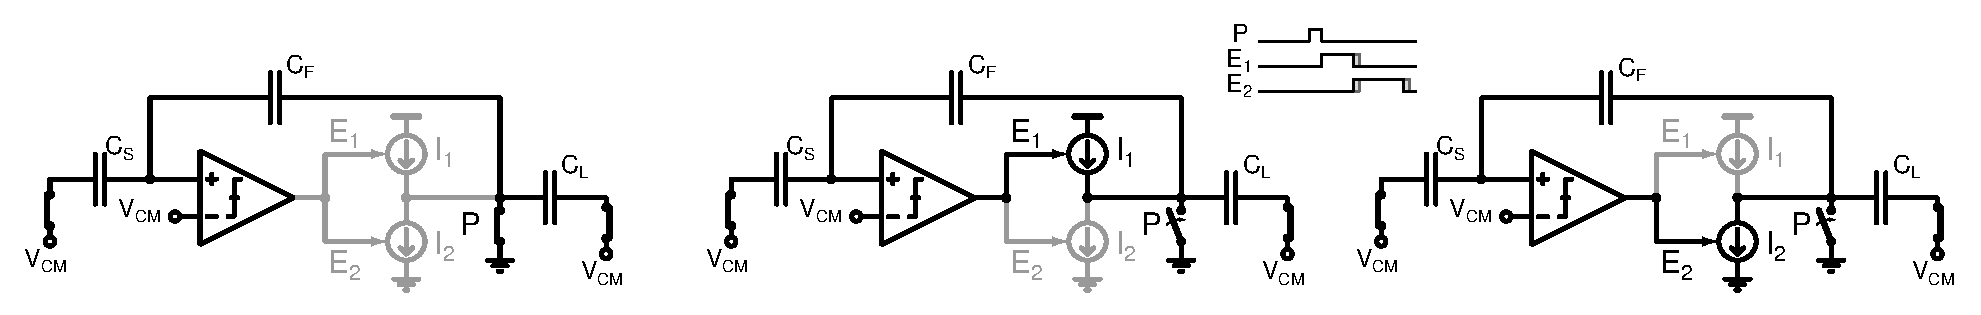
\includegraphics[width=\textwidth]{Chapter3/Figs/algo_comp_based.ps}
%	\caption{Comparator Based charge transfer}
%	\label{fig:algo_comp_based}
%\end{figure}

%\figurename~\ref{fig:algo_comp_based} represents how does the charges are transferred. The comparator inputs should be first shifted from their virtual ground condition to start a new transfer. In a second phase, the a large current ramp the output voltage in a similar way an amplifier slewing does. When the virtual ground is detected, the current source is turned off. Due to comparator's delay, an overshoot occurs. In third phase, a small current of opposite sign reverts the overshoot and get a more accurate measurement of the virtual ground condition turning off the second current source. This is similar to the linear behaviour of an amplifier.

%The accuracy of the settling is thus limited by the comparator's offset, the comparator resolution, the delay of the comparator, the slewing, the digital phase variations, and the noise in the third accurate phase~\cite{Fiorenza2006}.
%Folded flicker noise was found to be a significant contributor to the broadband noise: because the flicker noise of the comparator extends beyond the Nyquist rate of the converter~\cite{Sepke2008}. However, they exhibit less inherent noise than a traditional amplifier in a switched capacitor circuit~\cite{Fiorenza2006}.

%In the work of Brooks, a fully differential version have been proposed~\cite{Brooks2009}. Sensitive to current mismatch of process variation, this structure introduce as an extra offset not compensated worsen by the temperature. A chopper stabilization~\cite{Toth2003} and their alternatives can still be used to correct the introduced offset~\cite{Brooks2009}.
%Thence the limitation of the overshoot can be leveraged by ramping in only one direction~\cite{Lee2012}. This architecture blend power consumption, high speed even for very low power supply~\cite{Steyaert2012}.

%		\subsubsection{Ring Amplifier based}
%The digital phases being cumbersome, another amplifier emulation have been proposed: the Ring Amplifier. The Ring Amplifier is a three-stage inverter-based structure that have a large output swing, and its slew-based charging characterization makes it able to charge large capacitive load efficiently~\cite{Hershberg2012}.
%In closed loop configuration, the odd numbered stage structure is oscillating. A dead zone defined by design, kill the oscillation in a small zone around the trip point of the first inverter.
%The design of an accurate ring amplifier implies a tiny dead zone a few microvolts wherein output transistors are in sub-threshold. At the edge of the stability zone, and taking into consideration PVT variations, the dead zone is practically few millivolts. Despite this, it is found in several high speed, high accuracy ADCs~\cite{Hershberg2012,YLim2015,YLim2015FD,YCao2017}.

%The first improvement over~\cite{Hershberg2012} is found in~\cite{YLim2015} where the biasing is self-generated by an IR drop in the middle stage. The IR drop is realized by a resistance of few kilo-Ohms. Moreover, the final stage use high threshold voltage transistor to further improves the stability by increasing the dead zone. Unfortunately, the speed, the accuracy, and the stability is tightly coupled with the self-biasing resistance introduced.

%\begin{figure}[htp]
%	\centering
 %   \begin{subfigure}[b]{0.5\textwidth}
%        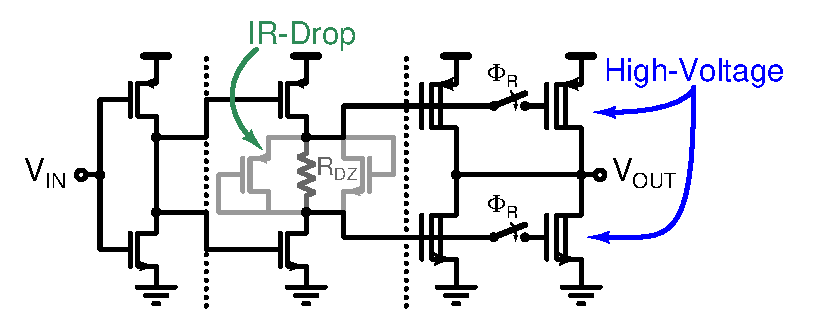
\includegraphics[width=\textwidth]{Chapter3/Figs/ring_amplifier_variations.ps}
%		\subcaption{variations}
%        \label{fig:ring_amp_variation}
%	\end{subfigure}
%	\begin{subfigure}[b]{0.48\textwidth}
%        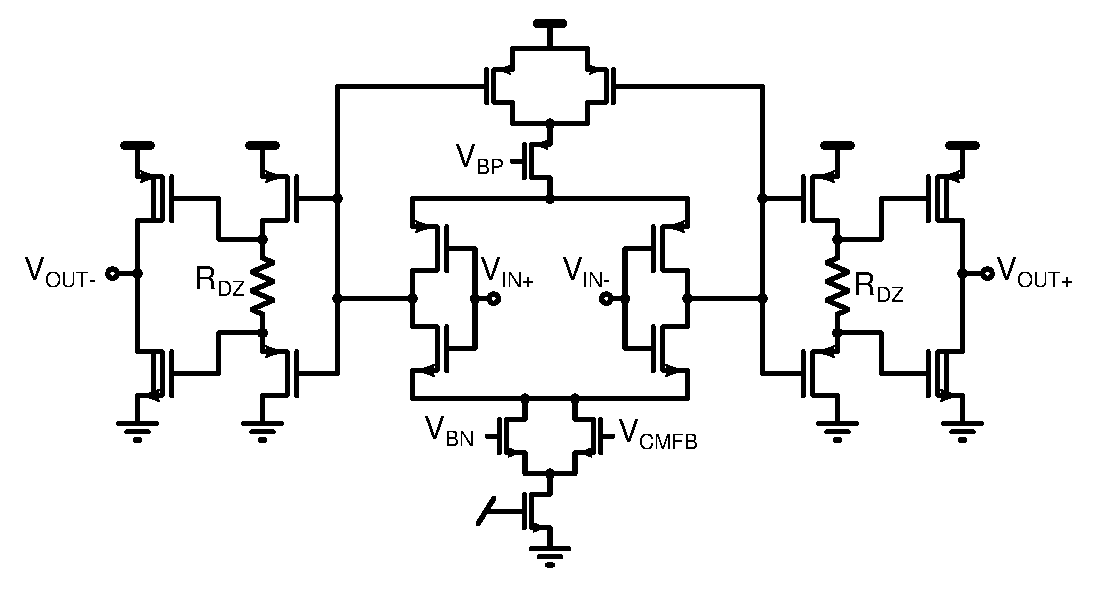
\includegraphics[width=\textwidth]{Chapter3/Figs/fully_diff_ring_amp.ps}
%        \subcaption{Fully-Differential Version}
%        \label{fig:ring_amp_fd}
%    \end{subfigure}
%	\caption[Ring Amplifier common variations]{Ring Amplifier common variations as in~\cite{YLim2015,YLim2015FD,YCao2017}}
%	\label{fig:algo_ring_amp}
%\end{figure}

%To improve the accuracy Megawer adds an auto-zero phase in which the complete ring amplifier is reset (shunt)~\cite{Megawer2016}. Both the input offset and output offset are thus ``trimmed''. To counter the fact that a reset of the fully ring amplifier generates a ring oscillator. The dead zone is thus enlarged to cut the oscillation path. To improve the efficiency, the final stage is changed to have a different slewing in the amplification phase and in the auto-zero phase. Sacrificing the speed by increasing the IR drop resistance, the IR drop is then changed into a common resistor for both amplification and auto-zero phase with an extra resistor for the auto-zero phase. The extra resistor is shorted during the amplification phase. These modifications result first into a linearity improvement for the same clock frequency in an area efficient way. But this revealed to compensate most of process variations.

%To cope with process and voltage variation, the IR drop resistance is replaced by diode connected transistors in~\cite{YCao2017}. Indeed, transistors have a decreased process variation compared to resistors, and connected as diodes the dead zone voltage variation is more stable.

%These disadvantages are those of a single ended structure which include the lack of inherent common mode and supply rejection, and the susceptibility to even orders of harmonics. The use of pseudo-differential structures and pseudo-differential common mode feedback (CMFB) can somewhat alleviate these problems~\cite{Hershberg2012,YLim2015}. Y. Lim and M. P. Flynn have even published a fully differential version of the ring amplifier in~\cite{YLim2015FD}.
%\nomenclature[z]{CMFB}{Common Mode Feedback}

%  The table~\ref{table:algo_comparison_table} highlights the main characteristics of the algorithmic converters.

%  \begin{table}[htp]
% 	\caption{Algorithmic-Pipelined ADC in the literature}
% 	\centering
% 	\label{table:algo_comparison_table}
% 	\begin{tabular}{L{3.5\charwidth} L{10\charwidth} R{7\charwidth} R{4.5\charwidth} R{4\charwidth} S[table-format=1.3,table-column-width=6\charwidth] R{6\charwidth} S[table-format=3.1,table-column-width=6\charwidth] C{3.5\charwidth}}
% 	\toprule
% 	Ref. & Architecture & Techno. [nm] & \(F_{snyq}\) [MHz] & OSR & {\makecell{{Area} \\ {[\(mm^2\)]}}} & Supply [V] & {\makecell{{Power} \\ {[mW]}}} & Res. \\
% 	\midrule
% 	\cite{YLim2015FD}  & pipe.-SAR &  65 &  50 & & 0.054 &  1.2 &   1   & 13 \\
% 	\cite{Murmann2003} & pipe.     & 350 &  75 & & 7.9   &  3   & 290   & 12 \\
% 	\cite{Lee2012}     & pipe.     &  65 &  50 & & 0.36  &  1   &   4   & 12 \\
% 	\cite{Lagos2017}   & pipe.     &  28 & 600 & & 0.62  &  0.9 &  14.2 & 12 \\
% 	\cite{Anderson2005} & pipe.    & 180 &  80 & & 1.9   &  1.8 &  94   & 10 \\
% 	\bottomrule
% 	\end{tabular}
% \end{table}
\newpage
\subsection{Successive Approximation Register} % section 2.5
\label{sec:sar-adc}
\nomenclature[z]{SAR}{Successive Approximation Register}
The first appearance of SAR ADC was back in early 70s~\cite{McCreary1975}. Using a binary search algorithm, this kind of converter is by far slower than a Flash or Folding ADC\@. As represented in \figurename~\ref{fig:sar_adc}, the SAR does not have any active component such an amplifier making it very efficient and targeting low-power application. But they are also able to perform either high-resolution conversions or high-speed conversions.

\begin{figure}[htp]
	\centering
	\begin{subfigure}[b]{0.44\textwidth}
		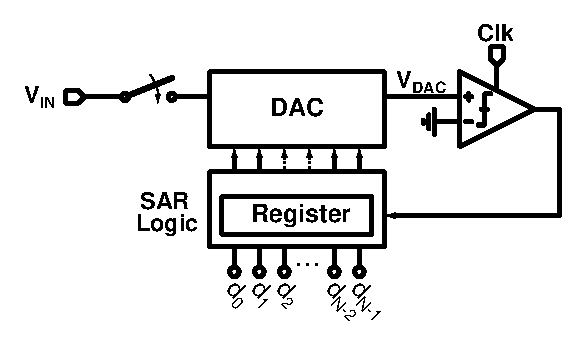
\includegraphics[width=\textwidth]{Chapter3/Figs/sar_principle.ps}
		\subcaption{principle}
		\label{fig:sar_principle}
	\end{subfigure}
	\begin{subfigure}[b]{0.52\textwidth}
		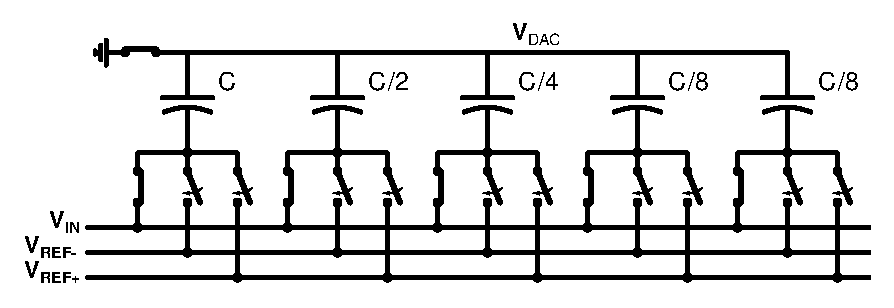
\includegraphics[width=\textwidth]{Chapter3/Figs/sar_classic_dac.ps}
		\subcaption{traditional DAC implementation}
		\label{fig:sar_dac_classical}
	\end{subfigure}
	\caption{Traditional charge redistribution SAR ADC as presented in~\cite{McCreary1975}}
	\label{fig:sar_adc}
\end{figure}

The architecture also benefits from using only one comparator to reduce the occupied area. With recent progress, the SAR converter outperforms other architectures in term of power consumption. Besides, its area occupancy has been tremendously shrunk, and the speed has been improved. Power dissipation sources are the digital control circuit, the comparator, and capacitive reference DAC network. The advancement in technology also favors the speed of the digital logic while the power consumption of the comparator and the capacitive DAC is limited by mismatch and noise~\cite{Yue2013,Mueller2013,Collins2017}. To address both the area occupancy and further reduce the energy consumption, the DAC architecture can be optimized by decreasing the capacitance and still preserving the binary scale.
\nomenclature[z]{DAC}{Digital-to-Analog Converter}

\subsubsection{DAC Enhancement}
Having high-resolution SAR ADC is quite challenging. Using a binary weighted capacitive reference in the DAC network leads to an increasing number of capacitors. Stereotypical capacitive DAC forms a binary scale split into a bunch of unit capacitors so that the n-th capacitor in the scale is a group of \(2^N\) of them. To increase the resolution from N to N+1, we double the number of unit capacitors. Thus, the occupied area grows exponentially as the resolution increases. And considering a differential structure, the phenomenon is even more pronounced causing lateral effects such as an excessive reference voltage loading.

Conventional techniques to shrink the area and to relax constraints on voltage buffers, designers usually play with serial-parallel configurations of unit components. This results in well-known techniques called split-junction and split-capacitor. The split-capacitor as represented in \figurename~\ref{fig:split_capacitor} inserts a capacitor which scales down a segment of the DAC\@. Thus, the biggest capacitors can be sized down to preserve the scale. The diminution of the load provides substantial power saving. The implementation obstacle is introduced by the attenuation capacitor not being multiple integers of the unit capacitor. Moreover, an extra switch per segmented DAC is introduced for the sampling of the input signal. Thus, the thermal noise is increased by both the scale down of capacitance and by the extra noise sources switches represent.

\begin{figure}[htp]
	\centering
	\begin{subfigure}[b]{0.46\textwidth}
		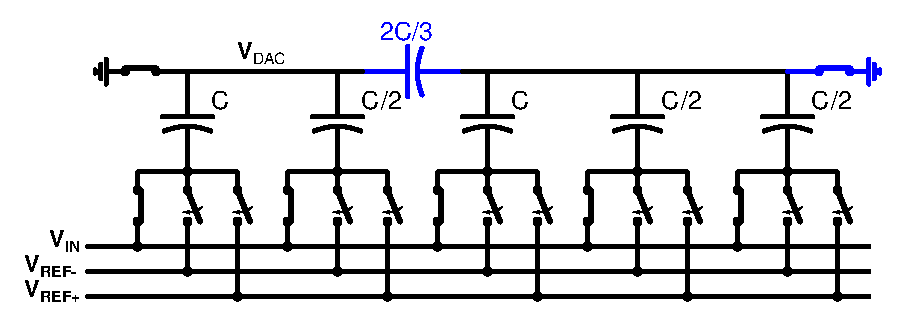
\includegraphics[width=\textwidth]{Chapter3/Figs/sar_split_cap_dac.ps}
		\subcaption{split capacitor}
		\label{fig:split_capacitor}
	\end{subfigure}
	\begin{subfigure}[b]{0.52\textwidth}
		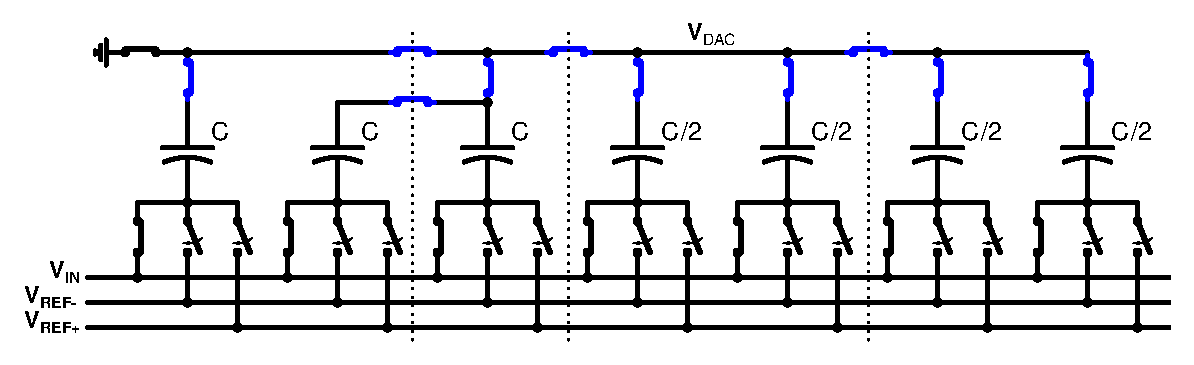
\includegraphics[width=\textwidth]{Chapter3/Figs/sar_split_junction_dac.ps}
		\subcaption{split junction}
		\label{fig:split_junction}
	\end{subfigure}
	\caption{DAC optimization by altering capacitors connections}
	\label{fig:sar_split_dac}
\end{figure}

Instead of connecting an attenuation capacitor in series to weight down part of the DAC to reduce the size of the biggest capacitors, small capacitors cunningly connected in parallel to split charges stored by the expected ratio. Introduced in~\cite{Lee2008} and optimized in~\cite{Yu2010}, the split junction scheme has a superior efficiency by reducing the number of ``down'' transitions by appending extra sections in parallel to redistribute charges. The two-step junction-splitting capacitor array requires more switches than the conventional and junction-splitting ones as depicted by the \figurename~\ref{fig:split_junction}. Compared to a classical DAC, this technique reduces the total capacitance by a factor \(2^{N/2}\) and has almost the same area saving than a split-capacitor method. From a thermal point of view, this architecture is more sensitive to thermal noise by adding noise source on the floating node \(V_{\rm DAC}\). The floating node connected to the comparator inputs leads to excessive decision error at high temperatures. Such error could be mitigated with the help of redundancy and non-binary ratio of the DAC scale~\cite{Zhang2014}.

\subsubsection{Switching Methods}
\label{sec:sar-switching}
The low-power asset of the SAR ADC can further be improved by a careful attention of switching energy loss. In the conventional charge-redistribution switching, the input voltage is sampled on all capacitors of the DAC during the first clock cycle. Then, we proceed in a voltage inversion and we remove half of the charges stored by connecting $V_{\rm refp}$ to one half and $V_{\rm refm}$ on the other half. Since this end of the capacitor is already at $V_{\rm inp}$ (resp. $V_{\rm inm}$), the energy is dissipated in switches to charge half of the capacitance and discharge the other half. In case the output bit $d_1 = 1$, the next capacitor is tested. As the weight of this capacitor is half of the previous one, there is less dissipation. Otherwise, the charge/discharge operation is reverting and the next capacitor is tested. The conventional charge-redistribution method is thus not power efficient owing to the discharge of the capacitor under test and charging-back this capacitor~\cite{Ginsburg2005}

\begin{figure}[htp]
	\centering
	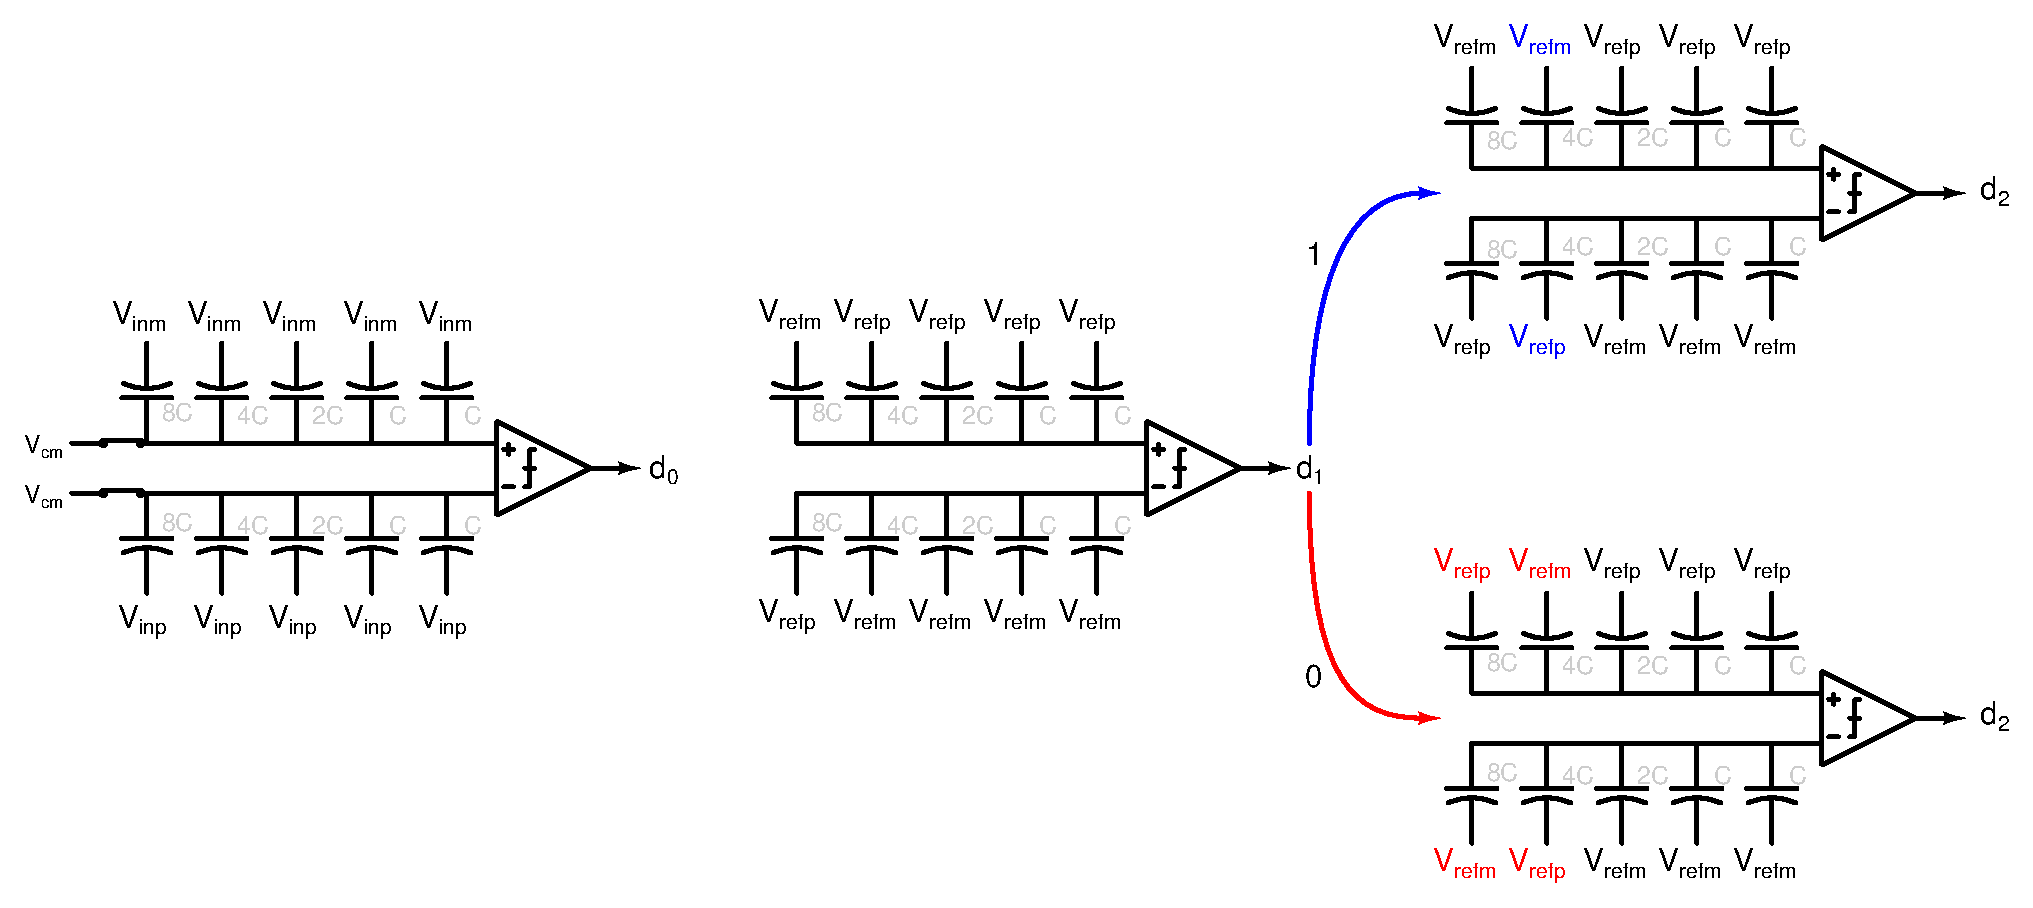
\includegraphics[width=\textwidth]{Chapter2/Figs/Vector/conv-charge-redis.ps}
	\caption{Traditional charge-redistribution conversion}
	\label{fig:sar_vcm_monotonic}
\end{figure}

Even if a lot of progress comes by a load reduction as discussed previously, the switching can strikingly reduce the power consumption; as far as 98\% of the conventional switching scheme~\cite{Zhu2013,Xie2014,Li2016}. The first technique which draws attention was the monotonic switching. Since the first clock cycle is the more power hungry, the monotonic switching samples the differential input voltage on the top-plates of capacitors while the common-mode voltage \(V_{\rm cm}\) is applied on the bottom-plates. As represented in \figurename~\ref{fig:sar_vcm_monotonic}, the comparator determines first bit \(d_0\) as polarity of the differential voltage~\cite{Ginsburg2005}. Compared to the conventional switching method, the reset of the MSB capacitor is saved. Moreover, an N-1 bits DAC is sufficient to output N-bits.  According to the comparison results, the logic unit will connect the largest capacitor of a bigger voltage side to the ground, and the other side remains the same. Therefore, almost half of the switching energy is saved. However, the common-mode level is decreasing during the monotonic switching, which puts a high demand on the performance of the comparator.

\begin{figure}[htp]
	\centering
	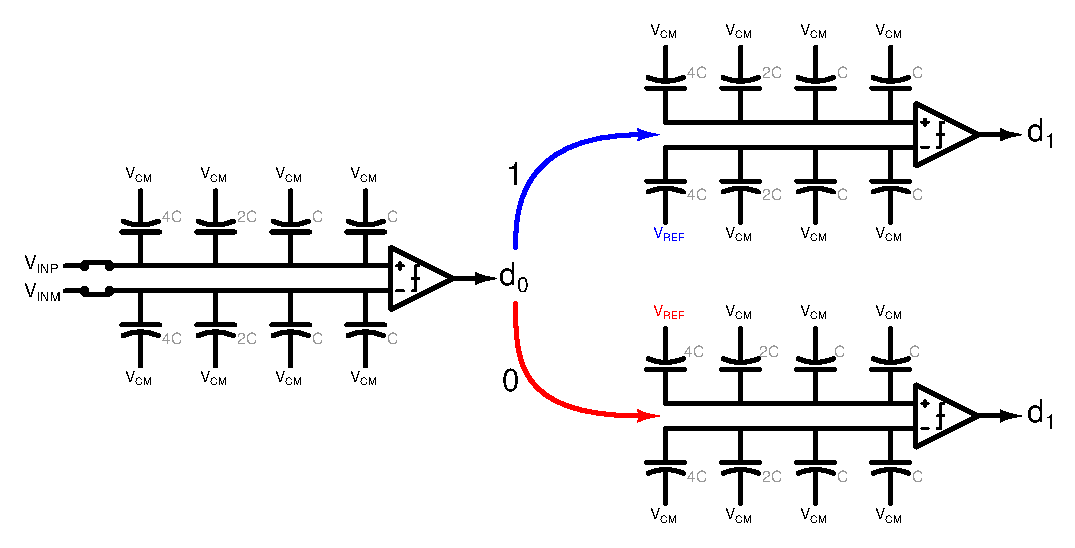
\includegraphics[width=0.8\textwidth]{Chapter3/Figs/sar_vcm_monotonic.ps}
	\caption{\(V_{\rm cm}\)-based monotonic digital switching to reduce area and save switching energy}
	\label{fig:sar_vcm_monotonic}
\end{figure}

Moreover, the switching loss is voltage dependent. The reduction of the voltage step diminishes the switching loss in the same proportion. Using \(V_{\rm cm}\) instead of the ground already halves the switching energy. In the sampling phase, the differential input is sampled as inputs on the top-plates (\(V_{\rm DAC}\)) while the bottom plates are connected to \(V_{\rm cm}\). After the sampling phase, during each conversion cycle of a \(V_{\rm cm}\)-based switching, the bottom plates of the capacitors will be switched in descending order, from \(V_{\rm cm}\) to \(V_{\rm refp}\) in one-side or another depending on each bit decision as depicted by \figurename~\ref{fig:sar_vcm_monotonic}. The connection to \(V_{\rm cm}\) adds one switch per capacitor increasing the thermal noise sources.

The switching being optimized, a further improvement could come from an assumption on the signal converted. As sensors outputs react slowly and their voltage usually filtered in front, the input signal of the ADC is of low mean activity over a time window. The conversion can start from an initial guess which is the output of the previous sample~\cite{Yaul2014}. Bit-cycling only last bits, the LSB first conversion performed is power efficient. When the error between the final code and the initial guess overtake few LSBs, a complete conversion shall be performed. Therefore, the power saving is inherent to the nature of the input signal. Without such an assumption, the power consumption is higher than previous methods and limits the speed of the conversion.

Compared to the traditional charge-redistribution scheme, these switching methods engender a large common-mode variation. This puts an extra design constraint on the comparator making a decision. For instance, the monotonic scheme allows only PMOS differential pairs which limit the maximum speed of comparison.

\subsubsection{Synchronous and Asynchronous Digital Implementation}
To optimize the digital circuitry, the clock rate is deeply linked to the power consumption. However, it conflicts with the specification for a manufacturable design. Indeed, the internal clock limits the settling time of DAC and the decision time of the comparator. For a robust design, one might base the sampling frequency on the peak delay in the worst corner. By using an asynchronous logic, such constraints could be relaxed on the comparator design. The conversion time \(T_{conv}  \) shall respect at least the following inequality
\begin{equation}
\label{eqn:sar_async_conv}
%\vcenter{\hbox{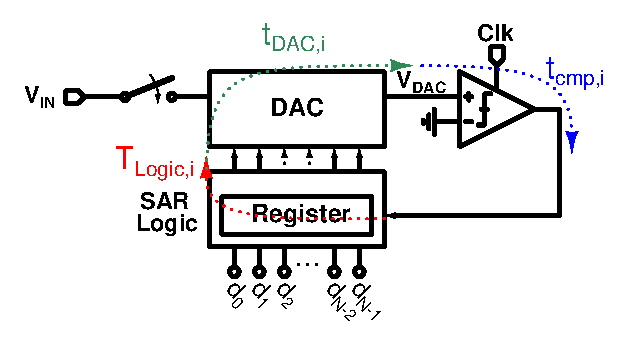
\includegraphics[width=0.45\textwidth]{sar_principle_timing.ps}}}
T_{conv} >= \sum_{i=0}^N {\textcolor{blue}{t_{cmp, i}}+\textcolor{red}{T_{Logic, i}}+\textcolor{Xgreen}{t_{DAC, i}}}
\end{equation}
where \(\textcolor{blue}{t_{cmp, i}}\) is the delay of the comparator, \(\textcolor{red}{T_{Logic, i}}\) the propagation time of the logic toggling switches, \(\textcolor{Xgreen}{t_{DAC, i}}\) the settling time of the DAC\@.

In a synchronous SAR, the two clock phases are used such that the first phase is dedicated to the DAC settling and the reset of the comparator whereas the second phase is devoted to the comparator decision and finish the settling. Also, the digital logic should control when the comparator resets and the moment to make a decision. With regard to the logic, a delay larger than the total delay from the comparator to the switching signals shall be ensured between a ready signal and the new decision start~\cite{Brenna2014}. By using a single XOR or NAND gate of the comparator outputs, a ready (valid) signal can be asserted~\cite{Brenna2014, Sekimoto2011, Zhu2015,Shen2018}. In turns, the ready signal triggers the reset of the comparator and the DAC settling. A delayed copy of the ready signal starts a new decision. This solution based on standard cells still requires delay cells. The delay sensitive to PVT variation, an asynchronous control is preferred. As done in \figurename~\ref{fig:sar_logic_jchen2011}, two loops can control respectively the reset and the next decision latching~\cite{JChen2011}. Unfortunately, the double-input T-flip-flop is not among standard cells in many processes. Moreover, the loop of the reset (in blue) should be ensured to be faster than the loop of the set (in red) over PVT variations after place and route. S.S. Wong \textit{et al.} presented switching signals to trigger the asynchronous loop instead of a fixed delay of comparator ready signal or asynchronous loop~\cite{Wong2013}. The process variation problem caused by the control logic and buffers is thus overcome without any tunable or worst-case delay cells. Represented in \figurename~\ref{fig:sar_logic_wong2013}, this also has the benefit of more easily ensure that DAC settling is started before triggering the comparator.

\begin{figure}[htp]
	\centering
	%\begin{subfigure}[b]{0.29\textwidth}
	%    \includegraphics[width=\textwidth]{sar_logic_Shen2018.ps}
	%    \subcaption{standard clock generation}
	%    \label{fig:sar_logic_basic}
	%\end{subfigure}
	\begin{subfigure}[b]{0.48\textwidth}
		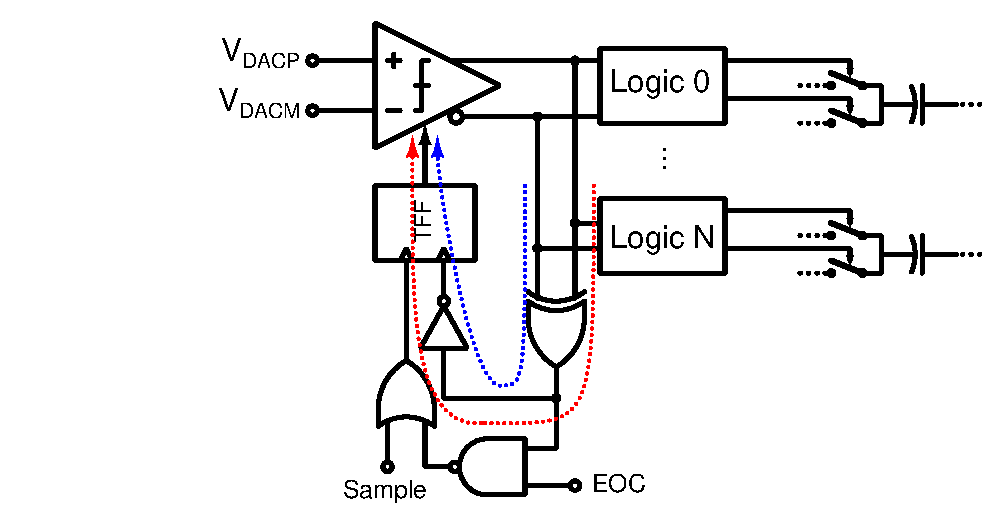
\includegraphics[width=\textwidth]{Chapter3/Figs/sar_logic_JChen2011.ps}
		\subcaption{separate clock/reset loop}
		\label{fig:sar_logic_jchen2011}
	\end{subfigure}
	\begin{subfigure}[b]{0.44\textwidth}
		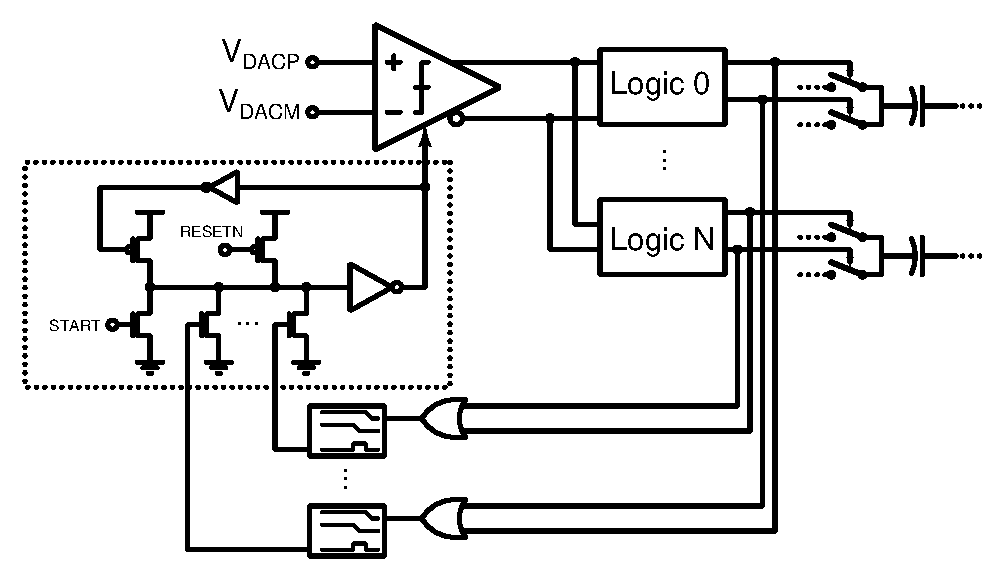
\includegraphics[width=\textwidth]{Chapter3/Figs/sar_logic_wong2013.ps}
		\subcaption{clock generation in~\cite{Wong2013}}
		\label{fig:sar_logic_wong2013}
	\end{subfigure}
	\caption{Comparator's clock generation}
	\label{fig:sar_cmp_clock}
\end{figure}

In addition, when the input voltages of the comparator are closer to each other, the comparator decision in either way to zero or one lasts longer. At low-temperature when the noise is not sufficient to force the latch in a state, metastability is inevitable. For unusually too long decision time, the digital code might be incomplete and result in errors. In the work of Tung \textit{et al.}, a timer circuit provides a timing slot which at the end a flag is raised to indicate the metastability and force the execution of subsequent cycles~\cite{Tung2016}. Moreover, the PVT variations alter the settling of the DAC\@. Instead of waiting for the full settling and sizing accordingly delay cells,~\cite{Kull2013} suggests that decision errors due to a partial settling can be tolerated with redundancy. An erroneous decision in the redundant region, via the non-binary scale of the DAC, is corrected by a later decision.

For the SAR logic, a shift register cadenced by ready (valid) signal is implemented and generates the end of conversion flag for the asynchronous clock generator~\cite{Brenna2014, Shen2018}. To the contrary, one could wait for the ready (valid) signal of the LSB logic as in~\cite{Wong2013}. The table~\ref{table:sar_comparison_table} gives as an abstract the main characteristics of these converters. Most of them achieved high speed and a low/medium resolution with fairly small power consumption.
\nomenclature[z]{MSB}{Most Significant Bit} \nomenclature[z]{LSB}{Least Significant Bit}
\begin{table}[htp]
	\caption{SAR ADC in the literature}
	\centering
	\label{table:sar_comparison_table}
	\begin{tabular}{L{3.5\charwidth} C{23\charwidth} R{6.5\charwidth} R{5\charwidth} S[table-format=2.2, table-column-width=5.2\charwidth] R{6\charwidth} R{5.5\charwidth} R{3.5\charwidth}}
		\toprule
		Ref. & Architecture & Techno. [nm] & \(F_{snyq}\) [MHz] & {\makecell{{Area}\\{[\(mm^2\)]}}} & Supply [V] & Power [\(\mu \)W] & Res. \tabularnewline \midrule
		\cite{Zhang2014} & 1.85-radix classic~CDAC   &  65 &  10 & 0.01 &  NA &   50 & 15 \\
		\cite{Shen2018}  & classic~CDAC asynchronous & 180 &  20 & 1.61 & 1.8 & 1770 & 12 \\
		\cite{Zhu2010}   & split-cap Vcm-based       &  90 & 100 & 0.18 & 1.2 & 3000 & 10 \\
		\cite{Liu2010}   & classic~CDAC Monotonic    & 130 &  50 & 0.05 & 1.2 &  826 & 10 \\
		\cite{Harpe2011} & classic~CDAC asynchronous &  90 &  10 & 0.05 &   1 &   26 &  8 \\
		\bottomrule
	\end{tabular}
\end{table}

In summary, a full-flash converter is a power hungry, and only one kind of ADC is not sufficient to reach high-resolution within 5-clock cycles. A cascade of sub-ADCs seems more promising. Architectures which suffer less from the analog deficiencies are $\Delta\Sigma$-based architectures, and the SAR\@. In addition to that, SAR ADCs using a charge redistribution are energy efficient. These are less limited by technology and supply voltage scaling compared to others.
However, in a $\Delta\Sigma$-based architecture, the re-use of an integrator outputs imposes important constraints on the amplifier. The latter should thus meet these over the full temperature range.

\clearpage
\section{Analog design under wide-temperature range}
\label{sec:temperature-analogue}

There are many industries such as the automotive that smart sensing and mixed signal electronics capable of operating within an extreme temperature range from -40 \(\degree \)C to 175 \(\degree \)C. At high temperatures, transistors suffer from several defects which degrade their performance which leads to the system performance variation.

Over such a large temperature range, physical phenomena due to temperature variation should be considered in the early design stages. The background presented in this section discusses the impact of the temperature on the device and circuit-level. Moreover, the material dependencies, as well as transistors variation with respect to the temperature, are illustrated with the CMOS XT018 technology results. % this last point should be discussed with JVE and PLA to respect technical disclosure.

\subsection{Physical limits}


\subsubsection{Energy Band Gap}        % section 2.1
\label{sec:bandgap}
In solid-state physics, the energy band gap is the energy required to supercharge an electron from the valence band to the conduction band. Any extra energy will change the thermodynamic equilibrium of the solid. Therefore, the electrons' state repartition in the valence and conduction band varies with the temperature according to the Fermi-Dirac distribution. Thus, the band-gap energy changes with respect to the temperature. These intrinsic properties are widely used for temperature sensing, voltage and current references, and temperature compensation circuits.

Even if, the fitting equations of low-temperature data have been greatly discussed~\cite{Varshni1967,Allen1976,Manoogian1979,Donnell1991}, the trend of the band-gap energy required over temperature is modeled easily by the Varshni equation~(\ref{eqn:Varshni}) in~\cite{Varshni1967}
\begin{equation}
\label{eqn:Varshni}
E_g(T) = E_g(T_0) - \alpha \frac{T^2}{T+\beta}
\end{equation}
\(E_g(T_0) \) represents the band gap energy required at the temperature of reference \(T_0 \), while \(\alpha \) and \(\beta \) are fitting constants. For the Silicon (Si), with \(T_0 = \)300 K, \(\alpha \) and \(\beta \) are respectively 0.473 meV/K and 636K. \(E_g(T_0) \) is given to be 1.166 eV. The change over the temperature range of interest is given by the \figurename~\ref{fig:bandgap} where the derivative with respect to the temperature is about 400 ppm/K.
\nomenclature[A-Eg]{$E_g$}{Bandgap Energy}
\nomenclature[A-K]{$K$}{degree Kelvin}
\nomenclature[A-K]{Si}{Silicon}

\begin{figure}[!ht]
	\centering
	%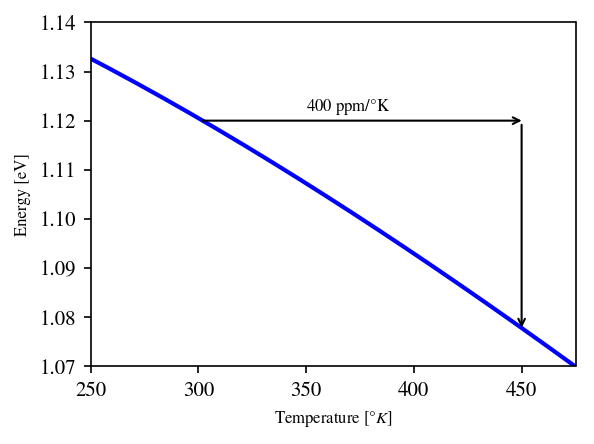
\includegraphics[width=0.6\textwidth]{bandgap}
	\resizebox{0.5\textwidth}{!}{
		%% Creator: Matplotlib, PGF backend
%%
%% To include the figure in your LaTeX document, write
%%   \input{<filename>.pgf}
%%
%% Make sure the required packages are loaded in your preamble
%%   \usepackage{pgf}
%%
%% Figures using additional raster images can only be included by \input if
%% they are in the same directory as the main LaTeX file. For loading figures
%% from other directories you can use the `import` package
%%   \usepackage{import}
%% and then include the figures with
%%   \import{<path to file>}{<filename>.pgf}
%%
%% Matplotlib used the following preamble
%%   \usepackage{gensymb}
%%   \usepackage[utf8x]{inputenc}
%%   \usepackage[T1]{fontenc}
%%
\begingroup%
\makeatletter%
\begin{pgfpicture}%
\pgfpathrectangle{\pgfpointorigin}{\pgfqpoint{3.930000in}{2.930000in}}%
\pgfusepath{use as bounding box, clip}%
\begin{pgfscope}%
\pgfsetbuttcap%
\pgfsetmiterjoin%
\definecolor{currentfill}{rgb}{1.000000,1.000000,1.000000}%
\pgfsetfillcolor{currentfill}%
\pgfsetlinewidth{0.000000pt}%
\definecolor{currentstroke}{rgb}{1.000000,1.000000,1.000000}%
\pgfsetstrokecolor{currentstroke}%
\pgfsetdash{}{0pt}%
\pgfpathmoveto{\pgfqpoint{0.000000in}{0.000000in}}%
\pgfpathlineto{\pgfqpoint{3.930000in}{0.000000in}}%
\pgfpathlineto{\pgfqpoint{3.930000in}{2.930000in}}%
\pgfpathlineto{\pgfqpoint{0.000000in}{2.930000in}}%
\pgfpathclose%
\pgfusepath{fill}%
\end{pgfscope}%
\begin{pgfscope}%
\pgfsetbuttcap%
\pgfsetmiterjoin%
\definecolor{currentfill}{rgb}{1.000000,1.000000,1.000000}%
\pgfsetfillcolor{currentfill}%
\pgfsetlinewidth{0.000000pt}%
\definecolor{currentstroke}{rgb}{0.000000,0.000000,0.000000}%
\pgfsetstrokecolor{currentstroke}%
\pgfsetstrokeopacity{0.000000}%
\pgfsetdash{}{0pt}%
\pgfpathmoveto{\pgfqpoint{0.624662in}{0.506458in}}%
\pgfpathlineto{\pgfqpoint{3.806667in}{0.506458in}}%
\pgfpathlineto{\pgfqpoint{3.806667in}{2.782172in}}%
\pgfpathlineto{\pgfqpoint{0.624662in}{2.782172in}}%
\pgfpathclose%
\pgfusepath{fill}%
\end{pgfscope}%
\begin{pgfscope}%
\pgfsetbuttcap%
\pgfsetroundjoin%
\definecolor{currentfill}{rgb}{0.000000,0.000000,0.000000}%
\pgfsetfillcolor{currentfill}%
\pgfsetlinewidth{0.803000pt}%
\definecolor{currentstroke}{rgb}{0.000000,0.000000,0.000000}%
\pgfsetstrokecolor{currentstroke}%
\pgfsetdash{}{0pt}%
\pgfsys@defobject{currentmarker}{\pgfqpoint{0.000000in}{-0.048611in}}{\pgfqpoint{0.000000in}{0.000000in}}{%
\pgfpathmoveto{\pgfqpoint{0.000000in}{0.000000in}}%
\pgfpathlineto{\pgfqpoint{0.000000in}{-0.048611in}}%
\pgfusepath{stroke,fill}%
}%
\begin{pgfscope}%
\pgfsys@transformshift{0.624662in}{0.506458in}%
\pgfsys@useobject{currentmarker}{}%
\end{pgfscope}%
\end{pgfscope}%
\begin{pgfscope}%
\pgftext[x=0.624662in,y=0.409236in,,top]{\fontsize{12.000000}{14.000000}\selectfont \(\displaystyle 250\)}%
\end{pgfscope}%
\begin{pgfscope}%
\pgfsetbuttcap%
\pgfsetroundjoin%
\definecolor{currentfill}{rgb}{0.000000,0.000000,0.000000}%
\pgfsetfillcolor{currentfill}%
\pgfsetlinewidth{0.803000pt}%
\definecolor{currentstroke}{rgb}{0.000000,0.000000,0.000000}%
\pgfsetstrokecolor{currentstroke}%
\pgfsetdash{}{0pt}%
\pgfsys@defobject{currentmarker}{\pgfqpoint{0.000000in}{-0.048611in}}{\pgfqpoint{0.000000in}{0.000000in}}{%
\pgfpathmoveto{\pgfqpoint{0.000000in}{0.000000in}}%
\pgfpathlineto{\pgfqpoint{0.000000in}{-0.048611in}}%
\pgfusepath{stroke,fill}%
}%
\begin{pgfscope}%
\pgfsys@transformshift{1.331774in}{0.506458in}%
\pgfsys@useobject{currentmarker}{}%
\end{pgfscope}%
\end{pgfscope}%
\begin{pgfscope}%
\pgftext[x=1.331774in,y=0.409236in,,top]{\fontsize{12.000000}{14.000000}\selectfont \(\displaystyle 300\)}%
\end{pgfscope}%
\begin{pgfscope}%
\pgfsetbuttcap%
\pgfsetroundjoin%
\definecolor{currentfill}{rgb}{0.000000,0.000000,0.000000}%
\pgfsetfillcolor{currentfill}%
\pgfsetlinewidth{0.803000pt}%
\definecolor{currentstroke}{rgb}{0.000000,0.000000,0.000000}%
\pgfsetstrokecolor{currentstroke}%
\pgfsetdash{}{0pt}%
\pgfsys@defobject{currentmarker}{\pgfqpoint{0.000000in}{-0.048611in}}{\pgfqpoint{0.000000in}{0.000000in}}{%
\pgfpathmoveto{\pgfqpoint{0.000000in}{0.000000in}}%
\pgfpathlineto{\pgfqpoint{0.000000in}{-0.048611in}}%
\pgfusepath{stroke,fill}%
}%
\begin{pgfscope}%
\pgfsys@transformshift{2.038886in}{0.506458in}%
\pgfsys@useobject{currentmarker}{}%
\end{pgfscope}%
\end{pgfscope}%
\begin{pgfscope}%
\pgftext[x=2.038886in,y=0.409236in,,top]{\fontsize{12.000000}{14.000000}\selectfont \(\displaystyle 350\)}%
\end{pgfscope}%
\begin{pgfscope}%
\pgfsetbuttcap%
\pgfsetroundjoin%
\definecolor{currentfill}{rgb}{0.000000,0.000000,0.000000}%
\pgfsetfillcolor{currentfill}%
\pgfsetlinewidth{0.803000pt}%
\definecolor{currentstroke}{rgb}{0.000000,0.000000,0.000000}%
\pgfsetstrokecolor{currentstroke}%
\pgfsetdash{}{0pt}%
\pgfsys@defobject{currentmarker}{\pgfqpoint{0.000000in}{-0.048611in}}{\pgfqpoint{0.000000in}{0.000000in}}{%
\pgfpathmoveto{\pgfqpoint{0.000000in}{0.000000in}}%
\pgfpathlineto{\pgfqpoint{0.000000in}{-0.048611in}}%
\pgfusepath{stroke,fill}%
}%
\begin{pgfscope}%
\pgfsys@transformshift{2.745998in}{0.506458in}%
\pgfsys@useobject{currentmarker}{}%
\end{pgfscope}%
\end{pgfscope}%
\begin{pgfscope}%
\pgftext[x=2.745998in,y=0.409236in,,top]{\fontsize{12.000000}{14.000000}\selectfont \(\displaystyle 400\)}%
\end{pgfscope}%
\begin{pgfscope}%
\pgfsetbuttcap%
\pgfsetroundjoin%
\definecolor{currentfill}{rgb}{0.000000,0.000000,0.000000}%
\pgfsetfillcolor{currentfill}%
\pgfsetlinewidth{0.803000pt}%
\definecolor{currentstroke}{rgb}{0.000000,0.000000,0.000000}%
\pgfsetstrokecolor{currentstroke}%
\pgfsetdash{}{0pt}%
\pgfsys@defobject{currentmarker}{\pgfqpoint{0.000000in}{-0.048611in}}{\pgfqpoint{0.000000in}{0.000000in}}{%
\pgfpathmoveto{\pgfqpoint{0.000000in}{0.000000in}}%
\pgfpathlineto{\pgfqpoint{0.000000in}{-0.048611in}}%
\pgfusepath{stroke,fill}%
}%
\begin{pgfscope}%
\pgfsys@transformshift{3.453111in}{0.506458in}%
\pgfsys@useobject{currentmarker}{}%
\end{pgfscope}%
\end{pgfscope}%
\begin{pgfscope}%
\pgftext[x=3.453111in,y=0.409236in,,top]{\fontsize{12.000000}{14.000000}\selectfont \(\displaystyle 450\)}%
\end{pgfscope}%
\begin{pgfscope}%
\pgftext[x=2.215664in,y=0.231025in,,top]{\fontsize{10.000000}{12.00000}\selectfont Temperature [K]}%
\end{pgfscope}%
\begin{pgfscope}%
\pgfsetbuttcap%
\pgfsetroundjoin%
\definecolor{currentfill}{rgb}{0.000000,0.000000,0.000000}%
\pgfsetfillcolor{currentfill}%
\pgfsetlinewidth{0.803000pt}%
\definecolor{currentstroke}{rgb}{0.000000,0.000000,0.000000}%
\pgfsetstrokecolor{currentstroke}%
\pgfsetdash{}{0pt}%
\pgfsys@defobject{currentmarker}{\pgfqpoint{-0.048611in}{0.000000in}}{\pgfqpoint{0.000000in}{0.000000in}}{%
\pgfpathmoveto{\pgfqpoint{0.000000in}{0.000000in}}%
\pgfpathlineto{\pgfqpoint{-0.048611in}{0.000000in}}%
\pgfusepath{stroke,fill}%
}%
\begin{pgfscope}%
\pgfsys@transformshift{0.624662in}{0.506458in}%
\pgfsys@useobject{currentmarker}{}%
\end{pgfscope}%
\end{pgfscope}%
\begin{pgfscope}%
\pgftext[x=0.280525in,y=0.458630in,left,base]{\fontsize{12.000000}{14.000000}\selectfont \(\displaystyle 1.07\)}%
\end{pgfscope}%
\begin{pgfscope}%
\pgfsetbuttcap%
\pgfsetroundjoin%
\definecolor{currentfill}{rgb}{0.000000,0.000000,0.000000}%
\pgfsetfillcolor{currentfill}%
\pgfsetlinewidth{0.803000pt}%
\definecolor{currentstroke}{rgb}{0.000000,0.000000,0.000000}%
\pgfsetstrokecolor{currentstroke}%
\pgfsetdash{}{0pt}%
\pgfsys@defobject{currentmarker}{\pgfqpoint{-0.048611in}{0.000000in}}{\pgfqpoint{0.000000in}{0.000000in}}{%
\pgfpathmoveto{\pgfqpoint{0.000000in}{0.000000in}}%
\pgfpathlineto{\pgfqpoint{-0.048611in}{0.000000in}}%
\pgfusepath{stroke,fill}%
}%
\begin{pgfscope}%
\pgfsys@transformshift{0.624662in}{0.831560in}%
\pgfsys@useobject{currentmarker}{}%
\end{pgfscope}%
\end{pgfscope}%
\begin{pgfscope}%
\pgftext[x=0.280525in,y=0.783732in,left,base]{\fontsize{12.000000}{14.000000}\selectfont \(\displaystyle 1.08\)}%
\end{pgfscope}%
\begin{pgfscope}%
\pgfsetbuttcap%
\pgfsetroundjoin%
\definecolor{currentfill}{rgb}{0.000000,0.000000,0.000000}%
\pgfsetfillcolor{currentfill}%
\pgfsetlinewidth{0.803000pt}%
\definecolor{currentstroke}{rgb}{0.000000,0.000000,0.000000}%
\pgfsetstrokecolor{currentstroke}%
\pgfsetdash{}{0pt}%
\pgfsys@defobject{currentmarker}{\pgfqpoint{-0.048611in}{0.000000in}}{\pgfqpoint{0.000000in}{0.000000in}}{%
\pgfpathmoveto{\pgfqpoint{0.000000in}{0.000000in}}%
\pgfpathlineto{\pgfqpoint{-0.048611in}{0.000000in}}%
\pgfusepath{stroke,fill}%
}%
\begin{pgfscope}%
\pgfsys@transformshift{0.624662in}{1.156662in}%
\pgfsys@useobject{currentmarker}{}%
\end{pgfscope}%
\end{pgfscope}%
\begin{pgfscope}%
\pgftext[x=0.280525in,y=1.108834in,left,base]{\fontsize{12.000000}{14.000000}\selectfont \(\displaystyle 1.09\)}%
\end{pgfscope}%
\begin{pgfscope}%
\pgfsetbuttcap%
\pgfsetroundjoin%
\definecolor{currentfill}{rgb}{0.000000,0.000000,0.000000}%
\pgfsetfillcolor{currentfill}%
\pgfsetlinewidth{0.803000pt}%
\definecolor{currentstroke}{rgb}{0.000000,0.000000,0.000000}%
\pgfsetstrokecolor{currentstroke}%
\pgfsetdash{}{0pt}%
\pgfsys@defobject{currentmarker}{\pgfqpoint{-0.048611in}{0.000000in}}{\pgfqpoint{0.000000in}{0.000000in}}{%
\pgfpathmoveto{\pgfqpoint{0.000000in}{0.000000in}}%
\pgfpathlineto{\pgfqpoint{-0.048611in}{0.000000in}}%
\pgfusepath{stroke,fill}%
}%
\begin{pgfscope}%
\pgfsys@transformshift{0.624662in}{1.481764in}%
\pgfsys@useobject{currentmarker}{}%
\end{pgfscope}%
\end{pgfscope}%
\begin{pgfscope}%
\pgftext[x=0.280525in,y=1.433936in,left,base]{\fontsize{12.000000}{14.000000}\selectfont \(\displaystyle 1.10\)}%
\end{pgfscope}%
\begin{pgfscope}%
\pgfsetbuttcap%
\pgfsetroundjoin%
\definecolor{currentfill}{rgb}{0.000000,0.000000,0.000000}%
\pgfsetfillcolor{currentfill}%
\pgfsetlinewidth{0.803000pt}%
\definecolor{currentstroke}{rgb}{0.000000,0.000000,0.000000}%
\pgfsetstrokecolor{currentstroke}%
\pgfsetdash{}{0pt}%
\pgfsys@defobject{currentmarker}{\pgfqpoint{-0.048611in}{0.000000in}}{\pgfqpoint{0.000000in}{0.000000in}}{%
\pgfpathmoveto{\pgfqpoint{0.000000in}{0.000000in}}%
\pgfpathlineto{\pgfqpoint{-0.048611in}{0.000000in}}%
\pgfusepath{stroke,fill}%
}%
\begin{pgfscope}%
\pgfsys@transformshift{0.624662in}{1.806866in}%
\pgfsys@useobject{currentmarker}{}%
\end{pgfscope}%
\end{pgfscope}%
\begin{pgfscope}%
\pgftext[x=0.280525in,y=1.759038in,left,base]{\fontsize{12.000000}{14.000000}\selectfont \(\displaystyle 1.11\)}%
\end{pgfscope}%
\begin{pgfscope}%
\pgfsetbuttcap%
\pgfsetroundjoin%
\definecolor{currentfill}{rgb}{0.000000,0.000000,0.000000}%
\pgfsetfillcolor{currentfill}%
\pgfsetlinewidth{0.803000pt}%
\definecolor{currentstroke}{rgb}{0.000000,0.000000,0.000000}%
\pgfsetstrokecolor{currentstroke}%
\pgfsetdash{}{0pt}%
\pgfsys@defobject{currentmarker}{\pgfqpoint{-0.048611in}{0.000000in}}{\pgfqpoint{0.000000in}{0.000000in}}{%
\pgfpathmoveto{\pgfqpoint{0.000000in}{0.000000in}}%
\pgfpathlineto{\pgfqpoint{-0.048611in}{0.000000in}}%
\pgfusepath{stroke,fill}%
}%
\begin{pgfscope}%
\pgfsys@transformshift{0.624662in}{2.131968in}%
\pgfsys@useobject{currentmarker}{}%
\end{pgfscope}%
\end{pgfscope}%
\begin{pgfscope}%
\pgftext[x=0.280525in,y=2.084140in,left,base]{\fontsize{12.000000}{14.000000}\selectfont \(\displaystyle 1.12\)}%
\end{pgfscope}%
\begin{pgfscope}%
\pgfsetbuttcap%
\pgfsetroundjoin%
\definecolor{currentfill}{rgb}{0.000000,0.000000,0.000000}%
\pgfsetfillcolor{currentfill}%
\pgfsetlinewidth{0.803000pt}%
\definecolor{currentstroke}{rgb}{0.000000,0.000000,0.000000}%
\pgfsetstrokecolor{currentstroke}%
\pgfsetdash{}{0pt}%
\pgfsys@defobject{currentmarker}{\pgfqpoint{-0.048611in}{0.000000in}}{\pgfqpoint{0.000000in}{0.000000in}}{%
\pgfpathmoveto{\pgfqpoint{0.000000in}{0.000000in}}%
\pgfpathlineto{\pgfqpoint{-0.048611in}{0.000000in}}%
\pgfusepath{stroke,fill}%
}%
\begin{pgfscope}%
\pgfsys@transformshift{0.624662in}{2.457070in}%
\pgfsys@useobject{currentmarker}{}%
\end{pgfscope}%
\end{pgfscope}%
\begin{pgfscope}%
\pgftext[x=0.280525in,y=2.409242in,left,base]{\fontsize{12.000000}{14.000000}\selectfont \(\displaystyle 1.13\)}%
\end{pgfscope}%
\begin{pgfscope}%
\pgfsetbuttcap%
\pgfsetroundjoin%
\definecolor{currentfill}{rgb}{0.000000,0.000000,0.000000}%
\pgfsetfillcolor{currentfill}%
\pgfsetlinewidth{0.803000pt}%
\definecolor{currentstroke}{rgb}{0.000000,0.000000,0.000000}%
\pgfsetstrokecolor{currentstroke}%
\pgfsetdash{}{0pt}%
\pgfsys@defobject{currentmarker}{\pgfqpoint{-0.048611in}{0.000000in}}{\pgfqpoint{0.000000in}{0.000000in}}{%
\pgfpathmoveto{\pgfqpoint{0.000000in}{0.000000in}}%
\pgfpathlineto{\pgfqpoint{-0.048611in}{0.000000in}}%
\pgfusepath{stroke,fill}%
}%
\begin{pgfscope}%
\pgfsys@transformshift{0.624662in}{2.782172in}%
\pgfsys@useobject{currentmarker}{}%
\end{pgfscope}%
\end{pgfscope}%
\begin{pgfscope}%
\pgftext[x=0.280525in,y=2.734344in,left,base]{\fontsize{12.000000}{14.000000}\selectfont \(\displaystyle 1.14\)}%
\end{pgfscope}%
\begin{pgfscope}%
\pgftext[x=0.224969in,y=1.644315in,,bottom,rotate=90.000000]{\fontsize{10.000000}{12.00000}\selectfont Energy [eV]}%
\end{pgfscope}%
\begin{pgfscope}%
\pgfpathrectangle{\pgfqpoint{0.624662in}{0.506458in}}{\pgfqpoint{3.182005in}{2.275714in}} %
\pgfusepath{clip}%
\pgfsetrectcap%
\pgfsetroundjoin%
\pgfsetlinewidth{2.007500pt}%
\definecolor{currentstroke}{rgb}{0.000000,0.000000,1.000000}%
\pgfsetstrokecolor{currentstroke}%
\pgfsetdash{}{0pt}%
\pgfpathmoveto{\pgfqpoint{0.617995in}{2.545919in}}%
\pgfpathlineto{\pgfqpoint{0.744228in}{2.479044in}}%
\pgfpathlineto{\pgfqpoint{0.921363in}{2.382473in}}%
\pgfpathlineto{\pgfqpoint{1.098498in}{2.283286in}}%
\pgfpathlineto{\pgfqpoint{1.275633in}{2.181588in}}%
\pgfpathlineto{\pgfqpoint{1.452769in}{2.077479in}}%
\pgfpathlineto{\pgfqpoint{1.629904in}{1.971054in}}%
\pgfpathlineto{\pgfqpoint{1.807039in}{1.862402in}}%
\pgfpathlineto{\pgfqpoint{1.984174in}{1.751609in}}%
\pgfpathlineto{\pgfqpoint{2.161309in}{1.638756in}}%
\pgfpathlineto{\pgfqpoint{2.338444in}{1.523919in}}%
\pgfpathlineto{\pgfqpoint{2.515580in}{1.407172in}}%
\pgfpathlineto{\pgfqpoint{2.692715in}{1.288583in}}%
\pgfpathlineto{\pgfqpoint{2.869850in}{1.168220in}}%
\pgfpathlineto{\pgfqpoint{3.046985in}{1.046146in}}%
\pgfpathlineto{\pgfqpoint{3.224120in}{0.922419in}}%
\pgfpathlineto{\pgfqpoint{3.401256in}{0.797099in}}%
\pgfpathlineto{\pgfqpoint{3.578391in}{0.670239in}}%
\pgfpathlineto{\pgfqpoint{3.755526in}{0.541892in}}%
\pgfpathlineto{\pgfqpoint{3.812986in}{0.499792in}}%
\pgfusepath{stroke}%
\end{pgfscope}%
\begin{pgfscope}%
\pgfsetrectcap%
\pgfsetmiterjoin%
\pgfsetlinewidth{0.803000pt}%
\definecolor{currentstroke}{rgb}{0.000000,0.000000,0.000000}%
\pgfsetstrokecolor{currentstroke}%
\pgfsetdash{}{0pt}%
\pgfpathmoveto{\pgfqpoint{0.624662in}{0.506458in}}%
\pgfpathlineto{\pgfqpoint{0.624662in}{2.782172in}}%
\pgfusepath{stroke}%
\end{pgfscope}%
\begin{pgfscope}%
\pgfsetrectcap%
\pgfsetmiterjoin%
\pgfsetlinewidth{0.803000pt}%
\definecolor{currentstroke}{rgb}{0.000000,0.000000,0.000000}%
\pgfsetstrokecolor{currentstroke}%
\pgfsetdash{}{0pt}%
\pgfpathmoveto{\pgfqpoint{3.806667in}{0.506458in}}%
\pgfpathlineto{\pgfqpoint{3.806667in}{2.782172in}}%
\pgfusepath{stroke}%
\end{pgfscope}%
\begin{pgfscope}%
\pgfsetrectcap%
\pgfsetmiterjoin%
\pgfsetlinewidth{0.803000pt}%
\definecolor{currentstroke}{rgb}{0.000000,0.000000,0.000000}%
\pgfsetstrokecolor{currentstroke}%
\pgfsetdash{}{0pt}%
\pgfpathmoveto{\pgfqpoint{0.624662in}{0.506458in}}%
\pgfpathlineto{\pgfqpoint{3.806667in}{0.506458in}}%
\pgfusepath{stroke}%
\end{pgfscope}%
\begin{pgfscope}%
\pgfsetrectcap%
\pgfsetmiterjoin%
\pgfsetlinewidth{0.803000pt}%
\definecolor{currentstroke}{rgb}{0.000000,0.000000,0.000000}%
\pgfsetstrokecolor{currentstroke}%
\pgfsetdash{}{0pt}%
\pgfpathmoveto{\pgfqpoint{0.624662in}{2.782172in}}%
\pgfpathlineto{\pgfqpoint{3.806667in}{2.782172in}}%
\pgfusepath{stroke}%
\end{pgfscope}%
\begin{pgfscope}%
\pgfsetroundcap%
\pgfsetroundjoin%
\pgfsetlinewidth{1.003750pt}%
\definecolor{currentstroke}{rgb}{0.000000,0.000000,0.000000}%
\pgfsetstrokecolor{currentstroke}%
\pgfsetdash{}{0pt}%
\pgfpathmoveto{\pgfqpoint{1.359556in}{2.131968in}}%
\pgfpathquadraticcurveto{\pgfqpoint{2.406602in}{2.131968in}}{\pgfqpoint{3.438120in}{2.131968in}}%
\pgfusepath{stroke}%
\end{pgfscope}%
\begin{pgfscope}%
\pgfsetroundcap%
\pgfsetroundjoin%
\pgfsetlinewidth{1.003750pt}%
\definecolor{currentstroke}{rgb}{0.000000,0.000000,0.000000}%
\pgfsetstrokecolor{currentstroke}%
\pgfsetdash{}{0pt}%
\pgfpathmoveto{\pgfqpoint{3.388120in}{2.156968in}}%
\pgfpathlineto{\pgfqpoint{3.438120in}{2.131968in}}%
\pgfpathlineto{\pgfqpoint{3.388120in}{2.106968in}}%
\pgfusepath{stroke}%
\end{pgfscope}%
\begin{pgfscope}%
\pgfsetroundcap%
\pgfsetroundjoin%
\pgfsetlinewidth{1.003750pt}%
\definecolor{currentstroke}{rgb}{0.000000,0.000000,0.000000}%
\pgfsetstrokecolor{currentstroke}%
\pgfsetdash{}{0pt}%
\pgfpathmoveto{\pgfqpoint{3.453111in}{2.104174in}}%
\pgfpathquadraticcurveto{\pgfqpoint{3.453111in}{1.432994in}}{\pgfqpoint{3.453111in}{0.777343in}}%
\pgfusepath{stroke}%
\end{pgfscope}%
\begin{pgfscope}%
\pgfsetroundcap%
\pgfsetroundjoin%
\pgfsetlinewidth{1.003750pt}%
\definecolor{currentstroke}{rgb}{0.000000,0.000000,0.000000}%
\pgfsetstrokecolor{currentstroke}%
\pgfsetdash{}{0pt}%
\pgfpathmoveto{\pgfqpoint{3.478111in}{0.827343in}}%
\pgfpathlineto{\pgfqpoint{3.453111in}{0.777343in}}%
\pgfpathlineto{\pgfqpoint{3.428111in}{0.827343in}}%
\pgfusepath{stroke}%
\end{pgfscope}%
\begin{pgfscope}%
\pgftext[x=2.038886in,y=2.196989in,left,base]{\fontsize{12.000000}{14.00000}\selectfont 400 ppm/K}%
\end{pgfscope}%
\end{pgfpicture}%
\makeatother%
\endgroup%

	}
	\caption{Band Gap Energy of the Silicon }
	\label{fig:bandgap}
\end{figure}

\subsubsection{Mobility}               % section 2.3
\label{sec:mobility}
Carriers in the doped semiconductor respond to any extra energy: one can accelerate them by the application of an electric field. The momentum gained is \(m_c v_c \) where \(v_c \) is the drift velocity. The factor of proportionality between the drift velocity and the electric field applied is called the mobility \(\mu_c \) in units of \(cm^2/V \). One should consider that any collision deflecting the carrier is limiting the velocity. Thus, the various scattering mechanisms limit the mobility.
\nomenclature[A-mu]{$\mu_i$}{mobility based on the phenomenon $i$ or of the particle $i$}

Therefore, the mobility has very complex temperature dependence, defined by the interaction of the following: phonon \(\mu_{ph} \), surface roughness \(\mu_{sr} \), bulk charge Coulombic \(\mu_{cb} \), and interface charge Coulombic  \(\mu_{int} \) scatterings. Each of these depends on the temperature and the electric field \(\xi_{eff} \).

The Berkeley Short-Channel IGFET Model (BSIM), one of the most widely used simulation models and the one of the technology used, combines these four scattering parameters into an effective mobility, \( \mu_{eff} \) using Matthiessen’s rule~(\ref{eqn:matthiessen}) \cite{Chain1997}.

\begin{equation}
\label{eqn:matthiessen}
\frac{1}{\mu_{eff}(T, \xi_{eff})} = \frac{1}{\mu_{ph}(T, \xi_{eff})} +
\frac{1}{\mu_{sr}(T, \xi_{eff})} + \frac{1}{\mu_{cb}(T, \xi_{eff})} +
\frac{1}{\mu_{int}(T, \xi_{eff})}
\end{equation}

The phonon scattering is a vibration of the crystal lattice. The temperature increasing carriers collision are more frequent. The mobility limitation at high temperature is dominated by this scattering mechanism. Theoretical analysis shows that the mobility due to lattice scattering will decrease in proportion to \(T^{-\frac{3}{2}} \).

Surface roughness scattering becomes dominant when high electric fields pull electrons closer to the Si/SiO2 surface (\(\mu_{sr} \varpropto \xi_{eff}^{-2.1} \))\cite{KLee1991}.

At low temperatures, electrons move more slowly, and lattice vibrations are
small. The ion impurity forces which have little impact on high-energy
particles become the dominant limit to mobility. In this regime, decreasing temperature extends the amount of time electrons spend passing an impurity ion, causing mobility to decrease as temperature decreases (\(\mu_{cb} \varpropto T \)).

At low temperatures, the interface charges have two conflicting dependencies. Reducing temperature reduces the carriers’ thermal velocity, which increases the impact of interface charges. However, the reduced thermal velocity also reduces the screening effect\cite{Jeon1989}, and this reduction in screening dominates the temperature dependence (\(\mu_{int} \varpropto T^{-1} \)). For a temperature greater than 200 K, the mobility is decreasing with the temperature increasing.

In the BSIM model of transistors, the mobility change over temperature is modeled as in the equation~(\ref{eqn:mobility_bsim}).

\begin{equation}
\label{eqn:mobility_bsim}
\mu_{eff}(T) \varpropto \mu_{eff}(T_0) {\left(\frac{T}{T_0} \right)}^{\alpha_\mu}
\end{equation}
\(T_0 \) is the room temperature (\(\approx 300 K \)) and \(\alpha_\mu \) is a fitting coefficient often set to $-1.5$ for NMOS transistors in strong inversion.

\subsubsection{Velocity Saturation}    % section 2.4
As presented in the Section~\ref{sec:mobility}, the mobility and the velocity of carriers are linked to each other as \(\nu \approx \mu \xi \); where \(\nu \) is the velocity, \(\mu \) the mobility, and \(\xi \) the electric field.

One assumption is that the mean free time of carriers between collisions is constant, which holds for low values of \(\xi \). But for high electric fields, the additional velocity component will result in a shorter average time between lattice scatterings, thus the mobility is no longer constant. An increase in energy no longer causes carrier velocity to increase; instead, the additional energy is lost to phonon generation through lattice interactions. The mobility will finally saturate for high electric fields, and it may be approximated by the following empirical expression:
\begin{equation}
\label{eqn:vsat}
\nu = \frac{\nu_s}{1 + \left(\frac{\xi}{\xi_{sat}}\right)}
\end{equation}
where \(\nu_s \) is the saturation velocity (\(10^7 \) cm/s for Si at 300 K), and \(\xi_{sat}\) is a constant equal to \(7.10^3 \) V/cm for electrons and \(2.10^4 \) V/cm for holes.

Although saturation velocity has been found to be a dominant temperature dependent parameter as far back as 1970~\cite{Fowler1970} using device as longer as 10 \(\mu \)m. In the BSIM4 device model, the impact of temperature on velocity saturation \(\nu_{sat} \) is modelled by~\cite{Chain1997} as:
\begin{equation}
\label{eqn:vsat_T}
\nu_{sat}(T) = \nu_{sat}(T_0) - \alpha_\nu \left(\frac{T}{T_0}-1\right)
\end{equation}
where \(\nu_{sat}(T_0)\) is the saturation velocity at nominal temperature (\(T_0 \)) and a \(\alpha_\nu \) is the saturation velocity temperature coefficient. Thus, the temperature degrades the saturation velocity and devices' current.

\subsubsection{Current Density}        % section 2.5
\label{sec:current_density}
The current densities relation related to the temperature it complex and based on two components given by the equation~(\ref{eqn:current_density}): the drift and the diffusion.

\begin{align}
\label{eqn:current_density}
J_N &= \textcolor{blue}{q\mu_n n \xi} + \textcolor{red}{qD_n\nabla n} \\
J_P &= \textcolor{blue}{q\mu_p p \xi} - \textcolor{red}{qD_p\nabla p}
\end{align}

The \textcolor{red}{diffusion} component corresponds to the displacement of carriers to even their concentration. The gradients of electrons and holes \(\nabla n \) and \(\nabla p \) are not dependent from the temperature. But the diffusion rates \(D_n \) and \(D_p \) are. Increasing the temperature increases particle kinetic energy, in turn, increasing the diffusion component of the total current.

The \textcolor{blue}{drift} component corresponds to the displacement of carriers under a force proportional to the electric field \(\xi \) and the mobility \(\mu_n \) and \(\mu_p \). The temperature impacts the mobility as related in Section~\ref{sec:mobility} and the carrier density as well. The carrier density is flat over temperature in the extrinsic region and the mobility is decreasing, one may deduce that drift current density decreases as the temperature increase.

The drift and diffusion currents have opposite temperature dependencies. The global trends of the current density over temperature will depend on the electric field applied.

Transistor's current density (\(J_{DS} = I_{DS}/W\)) increases as bias increases according to~\cite{Sze1981}:

\begin{equation}
J_{DS} = \mu \frac{\epsilon_{ox} \cdot \xi_{DS}}{L} \left(V_{GS}-V_{th}\right)
\label{eqn:JDS}
\end{equation}

Depending on transistor bias, \(J_{DS}\) is drift-dominated under the condition \(\xi_{DS} > \xi_{sat}\); but it is diffusion-dominated under the condition \(\xi_{DS} < \xi_{sat}\). In contrast to the bias dependency, \(J_{DS}\) has opposite temperature dependence while it is drift- and \allowbreak diffusion-dominated due to mobility scattering limitation. In fact, drift-dominated \(J_{DS}\) decreases, but diffusion-dominated \(J_{DS}\) increases as temperature increases.
\nomenclature[A-xi]{$\xi$}{electric field}

\begin{figure}[!ht]
	\centering
	%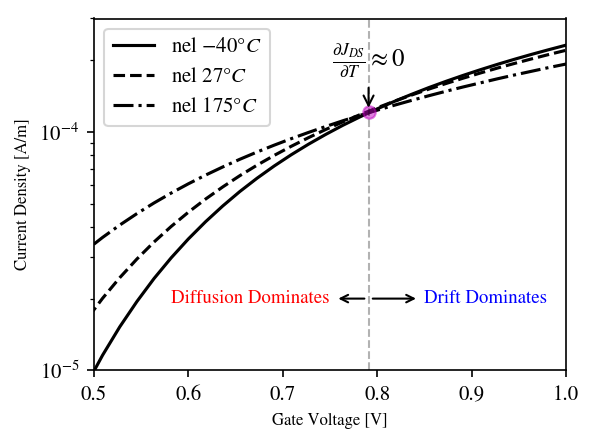
\includegraphics[width=0.6\textwidth]{jds_nel}
	%% Creator: Matplotlib, PGF backend
%%
%% To include the figure in your LaTeX document, write
%%   \input{<filename>.pgf}
%%
%% Make sure the required packages are loaded in your preamble
%%   \usepackage{pgf}
%%
%% Figures using additional raster images can only be included by \input if
%% they are in the same directory as the main LaTeX file. For loading figures
%% from other directories you can use the `import` package
%%   \usepackage{import}
%% and then include the figures with
%%   \import{<path to file>}{<filename>.pgf}
%%
%% Matplotlib used the following preamble
%%   \usepackage{gensymb}
%%   \usepackage[utf8x]{inputenc}
%%   \usepackage[T1]{fontenc}
%%
\begingroup%
\makeatletter%
\begin{pgfpicture}%
\pgfpathrectangle{\pgfpointorigin}{\pgfqpoint{3.930000in}{2.930000in}}%
\pgfusepath{use as bounding box, clip}%
\begin{pgfscope}%
\pgfsetbuttcap%
\pgfsetmiterjoin%
\definecolor{currentfill}{rgb}{1.000000,1.000000,1.000000}%
\pgfsetfillcolor{currentfill}%
\pgfsetlinewidth{0.000000pt}%
\definecolor{currentstroke}{rgb}{1.000000,1.000000,1.000000}%
\pgfsetstrokecolor{currentstroke}%
\pgfsetdash{}{0pt}%
\pgfpathmoveto{\pgfqpoint{0.000000in}{0.000000in}}%
\pgfpathlineto{\pgfqpoint{3.930000in}{0.000000in}}%
\pgfpathlineto{\pgfqpoint{3.930000in}{2.930000in}}%
\pgfpathlineto{\pgfqpoint{0.000000in}{2.930000in}}%
\pgfpathclose%
\pgfusepath{fill}%
\end{pgfscope}%
\begin{pgfscope}%
\pgfsetbuttcap%
\pgfsetmiterjoin%
\definecolor{currentfill}{rgb}{1.000000,1.000000,1.000000}%
\pgfsetfillcolor{currentfill}%
\pgfsetlinewidth{0.000000pt}%
\definecolor{currentstroke}{rgb}{0.000000,0.000000,0.000000}%
\pgfsetstrokecolor{currentstroke}%
\pgfsetstrokeopacity{0.000000}%
\pgfsetdash{}{0pt}%
\pgfpathmoveto{\pgfqpoint{0.665750in}{0.500402in}}%
\pgfpathlineto{\pgfqpoint{3.741265in}{0.500402in}}%
\pgfpathlineto{\pgfqpoint{3.741265in}{2.806667in}}%
\pgfpathlineto{\pgfqpoint{0.665750in}{2.806667in}}%
\pgfpathclose%
\pgfusepath{fill}%
\end{pgfscope}%
\begin{pgfscope}%
\pgfsetbuttcap%
\pgfsetroundjoin%
\definecolor{currentfill}{rgb}{0.000000,0.000000,0.000000}%
\pgfsetfillcolor{currentfill}%
\pgfsetlinewidth{0.803000pt}%
\definecolor{currentstroke}{rgb}{0.000000,0.000000,0.000000}%
\pgfsetstrokecolor{currentstroke}%
\pgfsetdash{}{0pt}%
\pgfsys@defobject{currentmarker}{\pgfqpoint{0.000000in}{-0.048611in}}{\pgfqpoint{0.000000in}{0.000000in}}{%
\pgfpathmoveto{\pgfqpoint{0.000000in}{0.000000in}}%
\pgfpathlineto{\pgfqpoint{0.000000in}{-0.048611in}}%
\pgfusepath{stroke,fill}%
}%
\begin{pgfscope}%
\pgfsys@transformshift{0.665750in}{0.500402in}%
\pgfsys@useobject{currentmarker}{}%
\end{pgfscope}%
\end{pgfscope}%
\begin{pgfscope}%
\pgftext[x=0.665750in,y=0.403180in,,top]{\fontsize{10.000000}{12.000000}\selectfont \(\displaystyle 0.5\)}%
\end{pgfscope}%
\begin{pgfscope}%
\pgfsetbuttcap%
\pgfsetroundjoin%
\definecolor{currentfill}{rgb}{0.000000,0.000000,0.000000}%
\pgfsetfillcolor{currentfill}%
\pgfsetlinewidth{0.803000pt}%
\definecolor{currentstroke}{rgb}{0.000000,0.000000,0.000000}%
\pgfsetstrokecolor{currentstroke}%
\pgfsetdash{}{0pt}%
\pgfsys@defobject{currentmarker}{\pgfqpoint{0.000000in}{-0.048611in}}{\pgfqpoint{0.000000in}{0.000000in}}{%
\pgfpathmoveto{\pgfqpoint{0.000000in}{0.000000in}}%
\pgfpathlineto{\pgfqpoint{0.000000in}{-0.048611in}}%
\pgfusepath{stroke,fill}%
}%
\begin{pgfscope}%
\pgfsys@transformshift{1.280853in}{0.500402in}%
\pgfsys@useobject{currentmarker}{}%
\end{pgfscope}%
\end{pgfscope}%
\begin{pgfscope}%
\pgftext[x=1.280853in,y=0.403180in,,top]{\fontsize{10.000000}{12.000000}\selectfont \(\displaystyle 0.6\)}%
\end{pgfscope}%
\begin{pgfscope}%
\pgfsetbuttcap%
\pgfsetroundjoin%
\definecolor{currentfill}{rgb}{0.000000,0.000000,0.000000}%
\pgfsetfillcolor{currentfill}%
\pgfsetlinewidth{0.803000pt}%
\definecolor{currentstroke}{rgb}{0.000000,0.000000,0.000000}%
\pgfsetstrokecolor{currentstroke}%
\pgfsetdash{}{0pt}%
\pgfsys@defobject{currentmarker}{\pgfqpoint{0.000000in}{-0.048611in}}{\pgfqpoint{0.000000in}{0.000000in}}{%
\pgfpathmoveto{\pgfqpoint{0.000000in}{0.000000in}}%
\pgfpathlineto{\pgfqpoint{0.000000in}{-0.048611in}}%
\pgfusepath{stroke,fill}%
}%
\begin{pgfscope}%
\pgfsys@transformshift{1.895956in}{0.500402in}%
\pgfsys@useobject{currentmarker}{}%
\end{pgfscope}%
\end{pgfscope}%
\begin{pgfscope}%
\pgftext[x=1.895956in,y=0.403180in,,top]{\fontsize{10.000000}{12.000000}\selectfont \(\displaystyle 0.7\)}%
\end{pgfscope}%
\begin{pgfscope}%
\pgfsetbuttcap%
\pgfsetroundjoin%
\definecolor{currentfill}{rgb}{0.000000,0.000000,0.000000}%
\pgfsetfillcolor{currentfill}%
\pgfsetlinewidth{0.803000pt}%
\definecolor{currentstroke}{rgb}{0.000000,0.000000,0.000000}%
\pgfsetstrokecolor{currentstroke}%
\pgfsetdash{}{0pt}%
\pgfsys@defobject{currentmarker}{\pgfqpoint{0.000000in}{-0.048611in}}{\pgfqpoint{0.000000in}{0.000000in}}{%
\pgfpathmoveto{\pgfqpoint{0.000000in}{0.000000in}}%
\pgfpathlineto{\pgfqpoint{0.000000in}{-0.048611in}}%
\pgfusepath{stroke,fill}%
}%
\begin{pgfscope}%
\pgfsys@transformshift{2.511059in}{0.500402in}%
\pgfsys@useobject{currentmarker}{}%
\end{pgfscope}%
\end{pgfscope}%
\begin{pgfscope}%
\pgftext[x=2.511059in,y=0.403180in,,top]{\fontsize{10.000000}{12.000000}\selectfont \(\displaystyle 0.8\)}%
\end{pgfscope}%
\begin{pgfscope}%
\pgfsetbuttcap%
\pgfsetroundjoin%
\definecolor{currentfill}{rgb}{0.000000,0.000000,0.000000}%
\pgfsetfillcolor{currentfill}%
\pgfsetlinewidth{0.803000pt}%
\definecolor{currentstroke}{rgb}{0.000000,0.000000,0.000000}%
\pgfsetstrokecolor{currentstroke}%
\pgfsetdash{}{0pt}%
\pgfsys@defobject{currentmarker}{\pgfqpoint{0.000000in}{-0.048611in}}{\pgfqpoint{0.000000in}{0.000000in}}{%
\pgfpathmoveto{\pgfqpoint{0.000000in}{0.000000in}}%
\pgfpathlineto{\pgfqpoint{0.000000in}{-0.048611in}}%
\pgfusepath{stroke,fill}%
}%
\begin{pgfscope}%
\pgfsys@transformshift{3.126162in}{0.500402in}%
\pgfsys@useobject{currentmarker}{}%
\end{pgfscope}%
\end{pgfscope}%
\begin{pgfscope}%
\pgftext[x=3.126162in,y=0.403180in,,top]{\fontsize{10.000000}{12.000000}\selectfont \(\displaystyle 0.9\)}%
\end{pgfscope}%
\begin{pgfscope}%
\pgfsetbuttcap%
\pgfsetroundjoin%
\definecolor{currentfill}{rgb}{0.000000,0.000000,0.000000}%
\pgfsetfillcolor{currentfill}%
\pgfsetlinewidth{0.803000pt}%
\definecolor{currentstroke}{rgb}{0.000000,0.000000,0.000000}%
\pgfsetstrokecolor{currentstroke}%
\pgfsetdash{}{0pt}%
\pgfsys@defobject{currentmarker}{\pgfqpoint{0.000000in}{-0.048611in}}{\pgfqpoint{0.000000in}{0.000000in}}{%
\pgfpathmoveto{\pgfqpoint{0.000000in}{0.000000in}}%
\pgfpathlineto{\pgfqpoint{0.000000in}{-0.048611in}}%
\pgfusepath{stroke,fill}%
}%
\begin{pgfscope}%
\pgfsys@transformshift{3.741265in}{0.500402in}%
\pgfsys@useobject{currentmarker}{}%
\end{pgfscope}%
\end{pgfscope}%
\begin{pgfscope}%
\pgftext[x=3.741265in,y=0.403180in,,top]{\fontsize{10.000000}{12.000000}\selectfont \(\displaystyle 1.0\)}%
\end{pgfscope}%
\begin{pgfscope}%
\pgftext[x=2.203507in,y=0.224969in,,top]{\fontsize{9.000000}{10.800000}\selectfont Gate Voltage [V]}%
\end{pgfscope}%
\begin{pgfscope}%
\pgfsetbuttcap%
\pgfsetroundjoin%
\definecolor{currentfill}{rgb}{0.000000,0.000000,0.000000}%
\pgfsetfillcolor{currentfill}%
\pgfsetlinewidth{0.803000pt}%
\definecolor{currentstroke}{rgb}{0.000000,0.000000,0.000000}%
\pgfsetstrokecolor{currentstroke}%
\pgfsetdash{}{0pt}%
\pgfsys@defobject{currentmarker}{\pgfqpoint{-0.048611in}{0.000000in}}{\pgfqpoint{0.000000in}{0.000000in}}{%
\pgfpathmoveto{\pgfqpoint{0.000000in}{0.000000in}}%
\pgfpathlineto{\pgfqpoint{-0.048611in}{0.000000in}}%
\pgfusepath{stroke,fill}%
}%
\begin{pgfscope}%
\pgfsys@transformshift{0.665750in}{0.500402in}%
\pgfsys@useobject{currentmarker}{}%
\end{pgfscope}%
\end{pgfscope}%
\begin{pgfscope}%
\pgftext[x=0.280525in,y=0.452575in,left,base]{\fontsize{10.000000}{12.000000}\selectfont \(\displaystyle 10^{-5}\)}%
\end{pgfscope}%
\begin{pgfscope}%
\pgfsetbuttcap%
\pgfsetroundjoin%
\definecolor{currentfill}{rgb}{0.000000,0.000000,0.000000}%
\pgfsetfillcolor{currentfill}%
\pgfsetlinewidth{0.803000pt}%
\definecolor{currentstroke}{rgb}{0.000000,0.000000,0.000000}%
\pgfsetstrokecolor{currentstroke}%
\pgfsetdash{}{0pt}%
\pgfsys@defobject{currentmarker}{\pgfqpoint{-0.048611in}{0.000000in}}{\pgfqpoint{0.000000in}{0.000000in}}{%
\pgfpathmoveto{\pgfqpoint{0.000000in}{0.000000in}}%
\pgfpathlineto{\pgfqpoint{-0.048611in}{0.000000in}}%
\pgfusepath{stroke,fill}%
}%
\begin{pgfscope}%
\pgfsys@transformshift{0.665750in}{2.061726in}%
\pgfsys@useobject{currentmarker}{}%
\end{pgfscope}%
\end{pgfscope}%
\begin{pgfscope}%
\pgftext[x=0.280525in,y=2.013898in,left,base]{\fontsize{10.000000}{12.000000}\selectfont \(\displaystyle 10^{-4}\)}%
\end{pgfscope}%
\begin{pgfscope}%
\pgfsetbuttcap%
\pgfsetroundjoin%
\definecolor{currentfill}{rgb}{0.000000,0.000000,0.000000}%
\pgfsetfillcolor{currentfill}%
\pgfsetlinewidth{0.602250pt}%
\definecolor{currentstroke}{rgb}{0.000000,0.000000,0.000000}%
\pgfsetstrokecolor{currentstroke}%
\pgfsetdash{}{0pt}%
\pgfsys@defobject{currentmarker}{\pgfqpoint{-0.027778in}{0.000000in}}{\pgfqpoint{0.000000in}{0.000000in}}{%
\pgfpathmoveto{\pgfqpoint{0.000000in}{0.000000in}}%
\pgfpathlineto{\pgfqpoint{-0.027778in}{0.000000in}}%
\pgfusepath{stroke,fill}%
}%
\begin{pgfscope}%
\pgfsys@transformshift{0.665750in}{0.970408in}%
\pgfsys@useobject{currentmarker}{}%
\end{pgfscope}%
\end{pgfscope}%
\begin{pgfscope}%
\pgfsetbuttcap%
\pgfsetroundjoin%
\definecolor{currentfill}{rgb}{0.000000,0.000000,0.000000}%
\pgfsetfillcolor{currentfill}%
\pgfsetlinewidth{0.602250pt}%
\definecolor{currentstroke}{rgb}{0.000000,0.000000,0.000000}%
\pgfsetstrokecolor{currentstroke}%
\pgfsetdash{}{0pt}%
\pgfsys@defobject{currentmarker}{\pgfqpoint{-0.027778in}{0.000000in}}{\pgfqpoint{0.000000in}{0.000000in}}{%
\pgfpathmoveto{\pgfqpoint{0.000000in}{0.000000in}}%
\pgfpathlineto{\pgfqpoint{-0.027778in}{0.000000in}}%
\pgfusepath{stroke,fill}%
}%
\begin{pgfscope}%
\pgfsys@transformshift{0.665750in}{1.245343in}%
\pgfsys@useobject{currentmarker}{}%
\end{pgfscope}%
\end{pgfscope}%
\begin{pgfscope}%
\pgfsetbuttcap%
\pgfsetroundjoin%
\definecolor{currentfill}{rgb}{0.000000,0.000000,0.000000}%
\pgfsetfillcolor{currentfill}%
\pgfsetlinewidth{0.602250pt}%
\definecolor{currentstroke}{rgb}{0.000000,0.000000,0.000000}%
\pgfsetstrokecolor{currentstroke}%
\pgfsetdash{}{0pt}%
\pgfsys@defobject{currentmarker}{\pgfqpoint{-0.027778in}{0.000000in}}{\pgfqpoint{0.000000in}{0.000000in}}{%
\pgfpathmoveto{\pgfqpoint{0.000000in}{0.000000in}}%
\pgfpathlineto{\pgfqpoint{-0.027778in}{0.000000in}}%
\pgfusepath{stroke,fill}%
}%
\begin{pgfscope}%
\pgfsys@transformshift{0.665750in}{1.440413in}%
\pgfsys@useobject{currentmarker}{}%
\end{pgfscope}%
\end{pgfscope}%
\begin{pgfscope}%
\pgfsetbuttcap%
\pgfsetroundjoin%
\definecolor{currentfill}{rgb}{0.000000,0.000000,0.000000}%
\pgfsetfillcolor{currentfill}%
\pgfsetlinewidth{0.602250pt}%
\definecolor{currentstroke}{rgb}{0.000000,0.000000,0.000000}%
\pgfsetstrokecolor{currentstroke}%
\pgfsetdash{}{0pt}%
\pgfsys@defobject{currentmarker}{\pgfqpoint{-0.027778in}{0.000000in}}{\pgfqpoint{0.000000in}{0.000000in}}{%
\pgfpathmoveto{\pgfqpoint{0.000000in}{0.000000in}}%
\pgfpathlineto{\pgfqpoint{-0.027778in}{0.000000in}}%
\pgfusepath{stroke,fill}%
}%
\begin{pgfscope}%
\pgfsys@transformshift{0.665750in}{1.591721in}%
\pgfsys@useobject{currentmarker}{}%
\end{pgfscope}%
\end{pgfscope}%
\begin{pgfscope}%
\pgfsetbuttcap%
\pgfsetroundjoin%
\definecolor{currentfill}{rgb}{0.000000,0.000000,0.000000}%
\pgfsetfillcolor{currentfill}%
\pgfsetlinewidth{0.602250pt}%
\definecolor{currentstroke}{rgb}{0.000000,0.000000,0.000000}%
\pgfsetstrokecolor{currentstroke}%
\pgfsetdash{}{0pt}%
\pgfsys@defobject{currentmarker}{\pgfqpoint{-0.027778in}{0.000000in}}{\pgfqpoint{0.000000in}{0.000000in}}{%
\pgfpathmoveto{\pgfqpoint{0.000000in}{0.000000in}}%
\pgfpathlineto{\pgfqpoint{-0.027778in}{0.000000in}}%
\pgfusepath{stroke,fill}%
}%
\begin{pgfscope}%
\pgfsys@transformshift{0.665750in}{1.715348in}%
\pgfsys@useobject{currentmarker}{}%
\end{pgfscope}%
\end{pgfscope}%
\begin{pgfscope}%
\pgfsetbuttcap%
\pgfsetroundjoin%
\definecolor{currentfill}{rgb}{0.000000,0.000000,0.000000}%
\pgfsetfillcolor{currentfill}%
\pgfsetlinewidth{0.602250pt}%
\definecolor{currentstroke}{rgb}{0.000000,0.000000,0.000000}%
\pgfsetstrokecolor{currentstroke}%
\pgfsetdash{}{0pt}%
\pgfsys@defobject{currentmarker}{\pgfqpoint{-0.027778in}{0.000000in}}{\pgfqpoint{0.000000in}{0.000000in}}{%
\pgfpathmoveto{\pgfqpoint{0.000000in}{0.000000in}}%
\pgfpathlineto{\pgfqpoint{-0.027778in}{0.000000in}}%
\pgfusepath{stroke,fill}%
}%
\begin{pgfscope}%
\pgfsys@transformshift{0.665750in}{1.819874in}%
\pgfsys@useobject{currentmarker}{}%
\end{pgfscope}%
\end{pgfscope}%
\begin{pgfscope}%
\pgfsetbuttcap%
\pgfsetroundjoin%
\definecolor{currentfill}{rgb}{0.000000,0.000000,0.000000}%
\pgfsetfillcolor{currentfill}%
\pgfsetlinewidth{0.602250pt}%
\definecolor{currentstroke}{rgb}{0.000000,0.000000,0.000000}%
\pgfsetstrokecolor{currentstroke}%
\pgfsetdash{}{0pt}%
\pgfsys@defobject{currentmarker}{\pgfqpoint{-0.027778in}{0.000000in}}{\pgfqpoint{0.000000in}{0.000000in}}{%
\pgfpathmoveto{\pgfqpoint{0.000000in}{0.000000in}}%
\pgfpathlineto{\pgfqpoint{-0.027778in}{0.000000in}}%
\pgfusepath{stroke,fill}%
}%
\begin{pgfscope}%
\pgfsys@transformshift{0.665750in}{1.910418in}%
\pgfsys@useobject{currentmarker}{}%
\end{pgfscope}%
\end{pgfscope}%
\begin{pgfscope}%
\pgfsetbuttcap%
\pgfsetroundjoin%
\definecolor{currentfill}{rgb}{0.000000,0.000000,0.000000}%
\pgfsetfillcolor{currentfill}%
\pgfsetlinewidth{0.602250pt}%
\definecolor{currentstroke}{rgb}{0.000000,0.000000,0.000000}%
\pgfsetstrokecolor{currentstroke}%
\pgfsetdash{}{0pt}%
\pgfsys@defobject{currentmarker}{\pgfqpoint{-0.027778in}{0.000000in}}{\pgfqpoint{0.000000in}{0.000000in}}{%
\pgfpathmoveto{\pgfqpoint{0.000000in}{0.000000in}}%
\pgfpathlineto{\pgfqpoint{-0.027778in}{0.000000in}}%
\pgfusepath{stroke,fill}%
}%
\begin{pgfscope}%
\pgfsys@transformshift{0.665750in}{1.990284in}%
\pgfsys@useobject{currentmarker}{}%
\end{pgfscope}%
\end{pgfscope}%
\begin{pgfscope}%
\pgfsetbuttcap%
\pgfsetroundjoin%
\definecolor{currentfill}{rgb}{0.000000,0.000000,0.000000}%
\pgfsetfillcolor{currentfill}%
\pgfsetlinewidth{0.602250pt}%
\definecolor{currentstroke}{rgb}{0.000000,0.000000,0.000000}%
\pgfsetstrokecolor{currentstroke}%
\pgfsetdash{}{0pt}%
\pgfsys@defobject{currentmarker}{\pgfqpoint{-0.027778in}{0.000000in}}{\pgfqpoint{0.000000in}{0.000000in}}{%
\pgfpathmoveto{\pgfqpoint{0.000000in}{0.000000in}}%
\pgfpathlineto{\pgfqpoint{-0.027778in}{0.000000in}}%
\pgfusepath{stroke,fill}%
}%
\begin{pgfscope}%
\pgfsys@transformshift{0.665750in}{2.531731in}%
\pgfsys@useobject{currentmarker}{}%
\end{pgfscope}%
\end{pgfscope}%
\begin{pgfscope}%
\pgfsetbuttcap%
\pgfsetroundjoin%
\definecolor{currentfill}{rgb}{0.000000,0.000000,0.000000}%
\pgfsetfillcolor{currentfill}%
\pgfsetlinewidth{0.602250pt}%
\definecolor{currentstroke}{rgb}{0.000000,0.000000,0.000000}%
\pgfsetstrokecolor{currentstroke}%
\pgfsetdash{}{0pt}%
\pgfsys@defobject{currentmarker}{\pgfqpoint{-0.027778in}{0.000000in}}{\pgfqpoint{0.000000in}{0.000000in}}{%
\pgfpathmoveto{\pgfqpoint{0.000000in}{0.000000in}}%
\pgfpathlineto{\pgfqpoint{-0.027778in}{0.000000in}}%
\pgfusepath{stroke,fill}%
}%
\begin{pgfscope}%
\pgfsys@transformshift{0.665750in}{2.806667in}%
\pgfsys@useobject{currentmarker}{}%
\end{pgfscope}%
\end{pgfscope}%
\begin{pgfscope}%
\pgftext[x=0.224969in,y=1.653535in,,bottom,rotate=90.000000]{\fontsize{9.000000}{10.800000}\selectfont Current Density [A/m]}%
\end{pgfscope}%
\begin{pgfscope}%
\pgfpathrectangle{\pgfqpoint{0.665750in}{0.500402in}}{\pgfqpoint{3.075515in}{2.306264in}} %
\pgfusepath{clip}%
\pgfsetrectcap%
\pgfsetroundjoin%
\pgfsetlinewidth{1.505625pt}%
\definecolor{currentstroke}{rgb}{0.000000,0.000000,0.000000}%
\pgfsetstrokecolor{currentstroke}%
\pgfsetdash{}{0pt}%
\pgfpathmoveto{\pgfqpoint{0.664776in}{0.493736in}}%
\pgfpathlineto{\pgfqpoint{0.721724in}{0.599286in}}%
\pgfpathlineto{\pgfqpoint{0.833673in}{0.785211in}}%
\pgfpathlineto{\pgfqpoint{0.945622in}{0.951499in}}%
\pgfpathlineto{\pgfqpoint{1.056955in}{1.101900in}}%
\pgfpathlineto{\pgfqpoint{1.168904in}{1.237843in}}%
\pgfpathlineto{\pgfqpoint{1.280853in}{1.361585in}}%
\pgfpathlineto{\pgfqpoint{1.392802in}{1.474303in}}%
\pgfpathlineto{\pgfqpoint{1.504750in}{1.577607in}}%
\pgfpathlineto{\pgfqpoint{1.616084in}{1.672309in}}%
\pgfpathlineto{\pgfqpoint{1.728033in}{1.759322in}}%
\pgfpathlineto{\pgfqpoint{1.839982in}{1.839635in}}%
\pgfpathlineto{\pgfqpoint{1.951930in}{1.913884in}}%
\pgfpathlineto{\pgfqpoint{2.063879in}{1.982707in}}%
\pgfpathlineto{\pgfqpoint{2.175828in}{2.046711in}}%
\pgfpathlineto{\pgfqpoint{2.287161in}{2.106335in}}%
\pgfpathlineto{\pgfqpoint{2.399110in}{2.161781in}}%
\pgfpathlineto{\pgfqpoint{2.511059in}{2.214118in}}%
\pgfpathlineto{\pgfqpoint{2.623008in}{2.263207in}}%
\pgfpathlineto{\pgfqpoint{2.734956in}{2.309452in}}%
\pgfpathlineto{\pgfqpoint{2.846290in}{2.353184in}}%
\pgfpathlineto{\pgfqpoint{2.958239in}{2.394266in}}%
\pgfpathlineto{\pgfqpoint{3.070188in}{2.433393in}}%
\pgfpathlineto{\pgfqpoint{3.182136in}{2.470385in}}%
\pgfpathlineto{\pgfqpoint{3.294085in}{2.505814in}}%
\pgfpathlineto{\pgfqpoint{3.406034in}{2.539485in}}%
\pgfpathlineto{\pgfqpoint{3.517368in}{2.571562in}}%
\pgfpathlineto{\pgfqpoint{3.629316in}{2.602190in}}%
\pgfpathlineto{\pgfqpoint{3.747932in}{2.633494in}}%
\pgfpathlineto{\pgfqpoint{3.747932in}{2.633494in}}%
\pgfusepath{stroke}%
\end{pgfscope}%
\begin{pgfscope}%
\pgfpathrectangle{\pgfqpoint{0.665750in}{0.500402in}}{\pgfqpoint{3.075515in}{2.306264in}} %
\pgfusepath{clip}%
\pgfsetbuttcap%
\pgfsetroundjoin%
\pgfsetlinewidth{1.505625pt}%
\definecolor{currentstroke}{rgb}{0.000000,0.000000,0.000000}%
\pgfsetstrokecolor{currentstroke}%
\pgfsetdash{{5.550000pt}{2.400000pt}}{0.000000pt}%
\pgfpathmoveto{\pgfqpoint{0.659083in}{0.888766in}}%
\pgfpathlineto{\pgfqpoint{0.721724in}{0.972439in}}%
\pgfpathlineto{\pgfqpoint{0.833673in}{1.107463in}}%
\pgfpathlineto{\pgfqpoint{0.945622in}{1.230028in}}%
\pgfpathlineto{\pgfqpoint{1.056955in}{1.341486in}}%
\pgfpathlineto{\pgfqpoint{1.168904in}{1.443457in}}%
\pgfpathlineto{\pgfqpoint{1.280853in}{1.536801in}}%
\pgfpathlineto{\pgfqpoint{1.392802in}{1.622864in}}%
\pgfpathlineto{\pgfqpoint{1.504750in}{1.702456in}}%
\pgfpathlineto{\pgfqpoint{1.616084in}{1.776267in}}%
\pgfpathlineto{\pgfqpoint{1.728033in}{1.844977in}}%
\pgfpathlineto{\pgfqpoint{1.839982in}{1.909146in}}%
\pgfpathlineto{\pgfqpoint{1.951930in}{1.969242in}}%
\pgfpathlineto{\pgfqpoint{2.063879in}{2.025731in}}%
\pgfpathlineto{\pgfqpoint{2.175828in}{2.079131in}}%
\pgfpathlineto{\pgfqpoint{2.287161in}{2.128815in}}%
\pgfpathlineto{\pgfqpoint{2.399110in}{2.176252in}}%
\pgfpathlineto{\pgfqpoint{2.511059in}{2.221122in}}%
\pgfpathlineto{\pgfqpoint{2.623008in}{2.264214in}}%
\pgfpathlineto{\pgfqpoint{2.734956in}{2.304730in}}%
\pgfpathlineto{\pgfqpoint{2.846290in}{2.343408in}}%
\pgfpathlineto{\pgfqpoint{2.958239in}{2.379999in}}%
\pgfpathlineto{\pgfqpoint{3.070188in}{2.415119in}}%
\pgfpathlineto{\pgfqpoint{3.182136in}{2.448892in}}%
\pgfpathlineto{\pgfqpoint{3.294085in}{2.481428in}}%
\pgfpathlineto{\pgfqpoint{3.406034in}{2.512125in}}%
\pgfpathlineto{\pgfqpoint{3.517368in}{2.541827in}}%
\pgfpathlineto{\pgfqpoint{3.629316in}{2.570602in}}%
\pgfpathlineto{\pgfqpoint{3.747932in}{2.599785in}}%
\pgfpathlineto{\pgfqpoint{3.747932in}{2.599785in}}%
\pgfusepath{stroke}%
\end{pgfscope}%
\begin{pgfscope}%
\pgfpathrectangle{\pgfqpoint{0.665750in}{0.500402in}}{\pgfqpoint{3.075515in}{2.306264in}} %
\pgfusepath{clip}%
\pgfsetbuttcap%
\pgfsetroundjoin%
\pgfsetlinewidth{1.505625pt}%
\definecolor{currentstroke}{rgb}{0.000000,0.000000,0.000000}%
\pgfsetstrokecolor{currentstroke}%
\pgfsetdash{{9.600000pt}{2.400000pt}{1.500000pt}{2.400000pt}}{0.000000pt}%
\pgfpathmoveto{\pgfqpoint{0.659083in}{1.322382in}}%
\pgfpathlineto{\pgfqpoint{0.721724in}{1.371415in}}%
\pgfpathlineto{\pgfqpoint{0.833673in}{1.452510in}}%
\pgfpathlineto{\pgfqpoint{0.945622in}{1.527622in}}%
\pgfpathlineto{\pgfqpoint{1.056955in}{1.597393in}}%
\pgfpathlineto{\pgfqpoint{1.168904in}{1.662362in}}%
\pgfpathlineto{\pgfqpoint{1.280853in}{1.723102in}}%
\pgfpathlineto{\pgfqpoint{1.392802in}{1.779976in}}%
\pgfpathlineto{\pgfqpoint{1.504750in}{1.833397in}}%
\pgfpathlineto{\pgfqpoint{1.616084in}{1.883708in}}%
\pgfpathlineto{\pgfqpoint{1.728033in}{1.931284in}}%
\pgfpathlineto{\pgfqpoint{1.839982in}{1.976354in}}%
\pgfpathlineto{\pgfqpoint{1.951930in}{2.019120in}}%
\pgfpathlineto{\pgfqpoint{2.063879in}{2.059825in}}%
\pgfpathlineto{\pgfqpoint{2.175828in}{2.098673in}}%
\pgfpathlineto{\pgfqpoint{2.287161in}{2.136145in}}%
\pgfpathlineto{\pgfqpoint{2.399110in}{2.171655in}}%
\pgfpathlineto{\pgfqpoint{2.511059in}{2.205397in}}%
\pgfpathlineto{\pgfqpoint{2.623008in}{2.238062in}}%
\pgfpathlineto{\pgfqpoint{2.734956in}{2.269725in}}%
\pgfpathlineto{\pgfqpoint{2.846290in}{2.299975in}}%
\pgfpathlineto{\pgfqpoint{2.958239in}{2.329390in}}%
\pgfpathlineto{\pgfqpoint{3.070188in}{2.357582in}}%
\pgfpathlineto{\pgfqpoint{3.294085in}{2.411081in}}%
\pgfpathlineto{\pgfqpoint{3.406034in}{2.436521in}}%
\pgfpathlineto{\pgfqpoint{3.629316in}{2.485070in}}%
\pgfpathlineto{\pgfqpoint{3.747932in}{2.509627in}}%
\pgfpathlineto{\pgfqpoint{3.747932in}{2.509627in}}%
\pgfusepath{stroke}%
\end{pgfscope}%
\begin{pgfscope}%
\pgfpathrectangle{\pgfqpoint{0.665750in}{0.500402in}}{\pgfqpoint{3.075515in}{2.306264in}} %
\pgfusepath{clip}%
\pgfsetbuttcap%
\pgfsetroundjoin%
\definecolor{currentfill}{rgb}{0.750000,0.000000,0.750000}%
\pgfsetfillcolor{currentfill}%
\pgfsetfillopacity{0.500000}%
\pgfsetlinewidth{1.003750pt}%
\definecolor{currentstroke}{rgb}{0.750000,0.000000,0.750000}%
\pgfsetstrokecolor{currentstroke}%
\pgfsetstrokeopacity{0.500000}%
\pgfsetdash{}{0pt}%
\pgfsys@defobject{currentmarker}{\pgfqpoint{-0.041667in}{-0.041667in}}{\pgfqpoint{0.041667in}{0.041667in}}{%
\pgfpathmoveto{\pgfqpoint{0.000000in}{-0.041667in}}%
\pgfpathcurveto{\pgfqpoint{0.011050in}{-0.041667in}}{\pgfqpoint{0.021649in}{-0.037276in}}{\pgfqpoint{0.029463in}{-0.029463in}}%
\pgfpathcurveto{\pgfqpoint{0.037276in}{-0.021649in}}{\pgfqpoint{0.041667in}{-0.011050in}}{\pgfqpoint{0.041667in}{0.000000in}}%
\pgfpathcurveto{\pgfqpoint{0.041667in}{0.011050in}}{\pgfqpoint{0.037276in}{0.021649in}}{\pgfqpoint{0.029463in}{0.029463in}}%
\pgfpathcurveto{\pgfqpoint{0.021649in}{0.037276in}}{\pgfqpoint{0.011050in}{0.041667in}}{\pgfqpoint{0.000000in}{0.041667in}}%
\pgfpathcurveto{\pgfqpoint{-0.011050in}{0.041667in}}{\pgfqpoint{-0.021649in}{0.037276in}}{\pgfqpoint{-0.029463in}{0.029463in}}%
\pgfpathcurveto{\pgfqpoint{-0.037276in}{0.021649in}}{\pgfqpoint{-0.041667in}{0.011050in}}{\pgfqpoint{-0.041667in}{0.000000in}}%
\pgfpathcurveto{\pgfqpoint{-0.041667in}{-0.011050in}}{\pgfqpoint{-0.037276in}{-0.021649in}}{\pgfqpoint{-0.029463in}{-0.029463in}}%
\pgfpathcurveto{\pgfqpoint{-0.021649in}{-0.037276in}}{\pgfqpoint{-0.011050in}{-0.041667in}}{\pgfqpoint{0.000000in}{-0.041667in}}%
\pgfpathclose%
\pgfusepath{stroke,fill}%
}%
\begin{pgfscope}%
\pgfsys@transformshift{2.455085in}{2.193654in}%
\pgfsys@useobject{currentmarker}{}%
\end{pgfscope}%
\end{pgfscope}%
\begin{pgfscope}%
\pgfpathrectangle{\pgfqpoint{0.665750in}{0.500402in}}{\pgfqpoint{3.075515in}{2.306264in}} %
\pgfusepath{clip}%
\pgfsetbuttcap%
\pgfsetroundjoin%
\pgfsetlinewidth{1.003750pt}%
\definecolor{currentstroke}{rgb}{0.000000,0.000000,0.000000}%
\pgfsetstrokecolor{currentstroke}%
\pgfsetstrokeopacity{0.300000}%
\pgfsetdash{{3.700000pt}{1.600000pt}}{0.000000pt}%
\pgfpathmoveto{\pgfqpoint{2.455085in}{0.500402in}}%
\pgfpathlineto{\pgfqpoint{2.455085in}{2.806667in}}%
\pgfusepath{stroke}%
\end{pgfscope}%
\begin{pgfscope}%
\pgfsetrectcap%
\pgfsetmiterjoin%
\pgfsetlinewidth{0.803000pt}%
\definecolor{currentstroke}{rgb}{0.000000,0.000000,0.000000}%
\pgfsetstrokecolor{currentstroke}%
\pgfsetdash{}{0pt}%
\pgfpathmoveto{\pgfqpoint{0.665750in}{0.500402in}}%
\pgfpathlineto{\pgfqpoint{0.665750in}{2.806667in}}%
\pgfusepath{stroke}%
\end{pgfscope}%
\begin{pgfscope}%
\pgfsetrectcap%
\pgfsetmiterjoin%
\pgfsetlinewidth{0.803000pt}%
\definecolor{currentstroke}{rgb}{0.000000,0.000000,0.000000}%
\pgfsetstrokecolor{currentstroke}%
\pgfsetdash{}{0pt}%
\pgfpathmoveto{\pgfqpoint{3.741265in}{0.500402in}}%
\pgfpathlineto{\pgfqpoint{3.741265in}{2.806667in}}%
\pgfusepath{stroke}%
\end{pgfscope}%
\begin{pgfscope}%
\pgfsetrectcap%
\pgfsetmiterjoin%
\pgfsetlinewidth{0.803000pt}%
\definecolor{currentstroke}{rgb}{0.000000,0.000000,0.000000}%
\pgfsetstrokecolor{currentstroke}%
\pgfsetdash{}{0pt}%
\pgfpathmoveto{\pgfqpoint{0.665750in}{0.500402in}}%
\pgfpathlineto{\pgfqpoint{3.741265in}{0.500402in}}%
\pgfusepath{stroke}%
\end{pgfscope}%
\begin{pgfscope}%
\pgfsetrectcap%
\pgfsetmiterjoin%
\pgfsetlinewidth{0.803000pt}%
\definecolor{currentstroke}{rgb}{0.000000,0.000000,0.000000}%
\pgfsetstrokecolor{currentstroke}%
\pgfsetdash{}{0pt}%
\pgfpathmoveto{\pgfqpoint{0.665750in}{2.806667in}}%
\pgfpathlineto{\pgfqpoint{3.741265in}{2.806667in}}%
\pgfusepath{stroke}%
\end{pgfscope}%
\begin{pgfscope}%
\pgfsetroundcap%
\pgfsetroundjoin%
\pgfsetlinewidth{1.003750pt}%
\definecolor{currentstroke}{rgb}{0.000000,0.000000,0.000000}%
\pgfsetstrokecolor{currentstroke}%
\pgfsetdash{}{0pt}%
\pgfpathmoveto{\pgfqpoint{2.455085in}{2.349939in}}%
\pgfpathquadraticcurveto{\pgfqpoint{2.455085in}{2.285695in}}{\pgfqpoint{2.455085in}{2.236979in}}%
\pgfusepath{stroke}%
\end{pgfscope}%
\begin{pgfscope}%
\pgfsetroundcap%
\pgfsetroundjoin%
\pgfsetlinewidth{1.003750pt}%
\definecolor{currentstroke}{rgb}{0.000000,0.000000,0.000000}%
\pgfsetstrokecolor{currentstroke}%
\pgfsetdash{}{0pt}%
\pgfpathmoveto{\pgfqpoint{2.480085in}{2.286979in}}%
\pgfpathlineto{\pgfqpoint{2.455085in}{2.236979in}}%
\pgfpathlineto{\pgfqpoint{2.430085in}{2.286979in}}%
\pgfusepath{stroke}%
\end{pgfscope}%
\begin{pgfscope}%
\pgftext[x=2.455085in,y=2.531731in,,]{\fontsize{9.000000}{10.800000}\selectfont \(\displaystyle \frac{\partial J_{DS}}{\partial T} \approx 0 \)}%
\end{pgfscope}%
\begin{pgfscope}%
\pgfsetroundcap%
\pgfsetroundjoin%
\pgfsetlinewidth{1.003750pt}%
\definecolor{currentstroke}{rgb}{0.000000,0.000000,0.000000}%
\pgfsetstrokecolor{currentstroke}%
\pgfsetdash{}{0pt}%
\pgfpathmoveto{\pgfqpoint{2.747536in}{0.970408in}}%
\pgfpathquadraticcurveto{\pgfqpoint{2.622956in}{0.970408in}}{\pgfqpoint{2.482849in}{0.970408in}}%
\pgfusepath{stroke}%
\end{pgfscope}%
\begin{pgfscope}%
\pgfsetroundcap%
\pgfsetroundjoin%
\pgfsetlinewidth{1.003750pt}%
\definecolor{currentstroke}{rgb}{0.000000,0.000000,0.000000}%
\pgfsetstrokecolor{currentstroke}%
\pgfsetdash{}{0pt}%
\pgfpathmoveto{\pgfqpoint{2.697536in}{0.995408in}}%
\pgfpathlineto{\pgfqpoint{2.747536in}{0.970408in}}%
\pgfpathlineto{\pgfqpoint{2.697536in}{0.945408in}}%
\pgfusepath{stroke}%
\end{pgfscope}%
\begin{pgfscope}%
\definecolor{textcolor}{rgb}{0.000000,0.000000,1.000000}%
\pgfsetstrokecolor{textcolor}%
\pgfsetfillcolor{textcolor}%
\pgftext[x=2.818611in,y=0.970408in,left,]{\color{textcolor}\fontsize{9.000000}{10.800000}\selectfont Drift Dominates}%
\end{pgfscope}%
\begin{pgfscope}%
\pgfsetroundcap%
\pgfsetroundjoin%
\pgfsetlinewidth{1.003750pt}%
\definecolor{currentstroke}{rgb}{0.000000,0.000000,0.000000}%
\pgfsetstrokecolor{currentstroke}%
\pgfsetdash{}{0pt}%
\pgfpathmoveto{\pgfqpoint{2.274597in}{0.970408in}}%
\pgfpathquadraticcurveto{\pgfqpoint{2.343187in}{0.970408in}}{\pgfqpoint{2.427304in}{0.970408in}}%
\pgfusepath{stroke}%
\end{pgfscope}%
\begin{pgfscope}%
\pgfsetroundcap%
\pgfsetroundjoin%
\pgfsetlinewidth{1.003750pt}%
\definecolor{currentstroke}{rgb}{0.000000,0.000000,0.000000}%
\pgfsetstrokecolor{currentstroke}%
\pgfsetdash{}{0pt}%
\pgfpathmoveto{\pgfqpoint{2.324597in}{0.945408in}}%
\pgfpathlineto{\pgfqpoint{2.274597in}{0.970408in}}%
\pgfpathlineto{\pgfqpoint{2.324597in}{0.995408in}}%
\pgfusepath{stroke}%
\end{pgfscope}%
\begin{pgfscope}%
\definecolor{textcolor}{rgb}{1.000000,0.000000,0.000000}%
\pgfsetstrokecolor{textcolor}%
\pgfsetfillcolor{textcolor}%
\pgftext[x=2.203507in,y=0.970408in,right,]{\color{textcolor}\fontsize{9.000000}{10.800000}\selectfont Diffusion Dominates}%
\end{pgfscope}%
\begin{pgfscope}%
\pgfsetbuttcap%
\pgfsetmiterjoin%
\definecolor{currentfill}{rgb}{1.000000,1.000000,1.000000}%
\pgfsetfillcolor{currentfill}%
\pgfsetfillopacity{0.800000}%
\pgfsetlinewidth{1.003750pt}%
\definecolor{currentstroke}{rgb}{0.800000,0.800000,0.800000}%
\pgfsetstrokecolor{currentstroke}%
\pgfsetstrokeopacity{0.800000}%
\pgfsetdash{}{0pt}%
\pgfpathmoveto{\pgfqpoint{0.762972in}{2.114557in}}%
\pgfpathlineto{\pgfqpoint{1.851093in}{2.114557in}}%
\pgfpathquadraticcurveto{\pgfqpoint{1.878871in}{2.114557in}}{\pgfqpoint{1.878871in}{2.142335in}}%
\pgfpathlineto{\pgfqpoint{1.878871in}{2.709444in}}%
\pgfpathquadraticcurveto{\pgfqpoint{1.878871in}{2.737222in}}{\pgfqpoint{1.851093in}{2.737222in}}%
\pgfpathlineto{\pgfqpoint{0.762972in}{2.737222in}}%
\pgfpathquadraticcurveto{\pgfqpoint{0.735194in}{2.737222in}}{\pgfqpoint{0.735194in}{2.709444in}}%
\pgfpathlineto{\pgfqpoint{0.735194in}{2.142335in}}%
\pgfpathquadraticcurveto{\pgfqpoint{0.735194in}{2.114557in}}{\pgfqpoint{0.762972in}{2.114557in}}%
\pgfpathclose%
\pgfusepath{stroke,fill}%
\end{pgfscope}%
\begin{pgfscope}%
\pgfsetrectcap%
\pgfsetroundjoin%
\pgfsetlinewidth{1.505625pt}%
\definecolor{currentstroke}{rgb}{0.000000,0.000000,0.000000}%
\pgfsetstrokecolor{currentstroke}%
\pgfsetdash{}{0pt}%
\pgfpathmoveto{\pgfqpoint{0.790750in}{2.633056in}}%
\pgfpathlineto{\pgfqpoint{1.068527in}{2.633056in}}%
\pgfusepath{stroke}%
\end{pgfscope}%
\begin{pgfscope}%
\pgftext[x=1.179639in,y=2.584444in,left,base]{\fontsize{10.000000}{12.000000}\selectfont nel \(\displaystyle -40 \degree C\)}%
\end{pgfscope}%
\begin{pgfscope}%
\pgfsetbuttcap%
\pgfsetroundjoin%
\pgfsetlinewidth{1.505625pt}%
\definecolor{currentstroke}{rgb}{0.000000,0.000000,0.000000}%
\pgfsetstrokecolor{currentstroke}%
\pgfsetdash{{5.550000pt}{2.400000pt}}{0.000000pt}%
\pgfpathmoveto{\pgfqpoint{0.790750in}{2.439389in}}%
\pgfpathlineto{\pgfqpoint{1.068527in}{2.439389in}}%
\pgfusepath{stroke}%
\end{pgfscope}%
\begin{pgfscope}%
\pgftext[x=1.179639in,y=2.390778in,left,base]{\fontsize{10.000000}{12.000000}\selectfont nel \(\displaystyle 27 \degree C\)}%
\end{pgfscope}%
\begin{pgfscope}%
\pgfsetbuttcap%
\pgfsetroundjoin%
\pgfsetlinewidth{1.505625pt}%
\definecolor{currentstroke}{rgb}{0.000000,0.000000,0.000000}%
\pgfsetstrokecolor{currentstroke}%
\pgfsetdash{{9.600000pt}{2.400000pt}{1.500000pt}{2.400000pt}}{0.000000pt}%
\pgfpathmoveto{\pgfqpoint{0.790750in}{2.245723in}}%
\pgfpathlineto{\pgfqpoint{1.068527in}{2.245723in}}%
\pgfusepath{stroke}%
\end{pgfscope}%
\begin{pgfscope}%
\pgftext[x=1.179639in,y=2.197112in,left,base]{\fontsize{10.000000}{12.000000}\selectfont nel \(\displaystyle 175 \degree C\)}%
\end{pgfscope}%
\end{pgfpicture}%
\makeatother%
\endgroup%

	\caption{Current density of low-VT nMOSFET of 1\(\mu \)m/180nm over temperature}
	\label{fig:jds_nel}
\end{figure}

To clarify the temperature variation, a simulation experiment is carried out using a n-type (\emph{nel}) low-\(V_{th}\) MOSFET of XT018 technology of XFAB\@. The \emph{nel} transistor is sized with \(W = 1 \mu \)m and \(L=180\) nm and the current density is represented at the \figurename~\ref{fig:jds_nel}. Another factor of current change over the temperature is the threshold voltage \(V_{th} \) in~(\ref{eqn:JDS}).

\subsubsection{Threshold Voltage}      % section 2.6
\label{sec:threshold}
The MOSFET threshold voltage is given in the equation~(\ref{eqn:thresold_fb_fermi})~\cite{Sze2006}, where \(V_{FB} \) is the voltage for which its application yields to a flat energy band in the semiconductor, \(\Phi_F \) is the Fermi energy, and \(\gamma \) the body effect parameters.
\begin{equation}
\label{eqn:thresold_fb_fermi}
V_{th} = V_{FB} + 2 \Phi_F + \gamma \sqrt{2 \Phi_F}
\end{equation}
\nomenclature[A-vth]{$V_{th}$}{transistor threshold voltage}
Its variation over temperature is found to be defined by~(\ref{eqn:thresold_fb_fermi_dT})~\cite{Filanovsky2001}.
\begin{equation}
\label{eqn:thresold_fb_fermi_dT}
\frac{\partial V_{th}}{\partial T} = \frac{\partial V_{FB}}{\partial T} + \left( 2  + \frac{\gamma}{\sqrt{2 \Phi_F}} \right) \frac{\partial \Phi_F}{\partial T}
\end{equation}

The flat band voltage depends on the dopant concentration of the substrate, of the gate, and the intrinsic carrier concentration of the silicon. The Fermi energy also changes over temperature as represented in \figurename~\ref{fig:electron_fermi_si}.

\begin{figure}[!ht]
	\centering
	%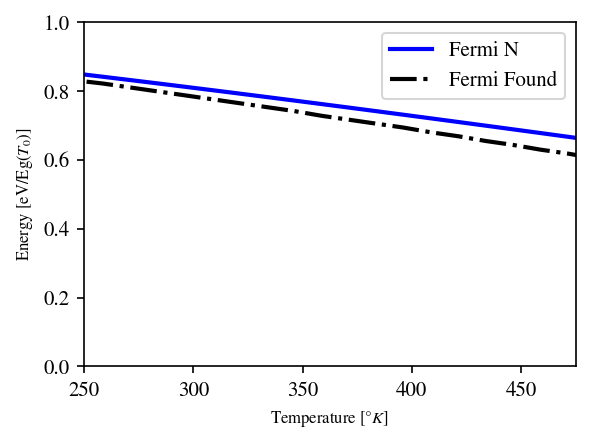
\includegraphics[width=0.6\textwidth]{fermi}
	\resizebox{0.5\textwidth}{!} {
		%% Creator: Matplotlib, PGF backend
%%
%% To include the figure in your LaTeX document, write
%%   \input{<filename>.pgf}
%%
%% Make sure the required packages are loaded in your preamble
%%   \usepackage{pgf}
%%
%% Figures using additional raster images can only be included by \input if
%% they are in the same directory as the main LaTeX file. For loading figures
%% from other directories you can use the `import` package
%%   \usepackage{import}
%% and then include the figures with
%%   \import{<path to file>}{<filename>.pgf}
%%
%% Matplotlib used the following preamble
%%   \usepackage{gensymb}
%%   \usepackage[utf8x]{inputenc}
%%   \usepackage[T1]{fontenc}
%%
\begingroup%
\makeatletter%
\begin{pgfpicture}%
\pgfpathrectangle{\pgfpointorigin}{\pgfqpoint{3.930000in}{2.930000in}}%
\pgfusepath{use as bounding box, clip}%
\begin{pgfscope}%
\pgfsetbuttcap%
\pgfsetmiterjoin%
\definecolor{currentfill}{rgb}{1.000000,1.000000,1.000000}%
\pgfsetfillcolor{currentfill}%
\pgfsetlinewidth{0.000000pt}%
\definecolor{currentstroke}{rgb}{1.000000,1.000000,1.000000}%
\pgfsetstrokecolor{currentstroke}%
\pgfsetdash{}{0pt}%
\pgfpathmoveto{\pgfqpoint{0.000000in}{0.000000in}}%
\pgfpathlineto{\pgfqpoint{3.930000in}{0.000000in}}%
\pgfpathlineto{\pgfqpoint{3.930000in}{2.930000in}}%
\pgfpathlineto{\pgfqpoint{0.000000in}{2.930000in}}%
\pgfpathclose%
\pgfusepath{fill}%
\end{pgfscope}%
\begin{pgfscope}%
\pgfsetbuttcap%
\pgfsetmiterjoin%
\definecolor{currentfill}{rgb}{1.000000,1.000000,1.000000}%
\pgfsetfillcolor{currentfill}%
\pgfsetlinewidth{0.000000pt}%
\definecolor{currentstroke}{rgb}{0.000000,0.000000,0.000000}%
\pgfsetstrokecolor{currentstroke}%
\pgfsetstrokeopacity{0.000000}%
\pgfsetdash{}{0pt}%
\pgfpathmoveto{\pgfqpoint{0.555217in}{0.506458in}}%
\pgfpathlineto{\pgfqpoint{3.806667in}{0.506458in}}%
\pgfpathlineto{\pgfqpoint{3.806667in}{2.782172in}}%
\pgfpathlineto{\pgfqpoint{0.555217in}{2.782172in}}%
\pgfpathclose%
\pgfusepath{fill}%
\end{pgfscope}%
\begin{pgfscope}%
\pgfsetbuttcap%
\pgfsetroundjoin%
\definecolor{currentfill}{rgb}{0.000000,0.000000,0.000000}%
\pgfsetfillcolor{currentfill}%
\pgfsetlinewidth{0.803000pt}%
\definecolor{currentstroke}{rgb}{0.000000,0.000000,0.000000}%
\pgfsetstrokecolor{currentstroke}%
\pgfsetdash{}{0pt}%
\pgfsys@defobject{currentmarker}{\pgfqpoint{0.000000in}{-0.048611in}}{\pgfqpoint{0.000000in}{0.000000in}}{%
\pgfpathmoveto{\pgfqpoint{0.000000in}{0.000000in}}%
\pgfpathlineto{\pgfqpoint{0.000000in}{-0.048611in}}%
\pgfusepath{stroke,fill}%
}%
\begin{pgfscope}%
\pgfsys@transformshift{0.555217in}{0.506458in}%
\pgfsys@useobject{currentmarker}{}%
\end{pgfscope}%
\end{pgfscope}%
\begin{pgfscope}%
\pgftext[x=0.555217in,y=0.409236in,,top]{\fontsize{12.000000}{14.000000}\selectfont \(\displaystyle 250\)}%
\end{pgfscope}%
\begin{pgfscope}%
\pgfsetbuttcap%
\pgfsetroundjoin%
\definecolor{currentfill}{rgb}{0.000000,0.000000,0.000000}%
\pgfsetfillcolor{currentfill}%
\pgfsetlinewidth{0.803000pt}%
\definecolor{currentstroke}{rgb}{0.000000,0.000000,0.000000}%
\pgfsetstrokecolor{currentstroke}%
\pgfsetdash{}{0pt}%
\pgfsys@defobject{currentmarker}{\pgfqpoint{0.000000in}{-0.048611in}}{\pgfqpoint{0.000000in}{0.000000in}}{%
\pgfpathmoveto{\pgfqpoint{0.000000in}{0.000000in}}%
\pgfpathlineto{\pgfqpoint{0.000000in}{-0.048611in}}%
\pgfusepath{stroke,fill}%
}%
\begin{pgfscope}%
\pgfsys@transformshift{1.277761in}{0.506458in}%
\pgfsys@useobject{currentmarker}{}%
\end{pgfscope}%
\end{pgfscope}%
\begin{pgfscope}%
\pgftext[x=1.277761in,y=0.409236in,,top]{\fontsize{12.000000}{14.000000}\selectfont \(\displaystyle 300\)}%
\end{pgfscope}%
\begin{pgfscope}%
\pgfsetbuttcap%
\pgfsetroundjoin%
\definecolor{currentfill}{rgb}{0.000000,0.000000,0.000000}%
\pgfsetfillcolor{currentfill}%
\pgfsetlinewidth{0.803000pt}%
\definecolor{currentstroke}{rgb}{0.000000,0.000000,0.000000}%
\pgfsetstrokecolor{currentstroke}%
\pgfsetdash{}{0pt}%
\pgfsys@defobject{currentmarker}{\pgfqpoint{0.000000in}{-0.048611in}}{\pgfqpoint{0.000000in}{0.000000in}}{%
\pgfpathmoveto{\pgfqpoint{0.000000in}{0.000000in}}%
\pgfpathlineto{\pgfqpoint{0.000000in}{-0.048611in}}%
\pgfusepath{stroke,fill}%
}%
\begin{pgfscope}%
\pgfsys@transformshift{2.000306in}{0.506458in}%
\pgfsys@useobject{currentmarker}{}%
\end{pgfscope}%
\end{pgfscope}%
\begin{pgfscope}%
\pgftext[x=2.000306in,y=0.409236in,,top]{\fontsize{12.000000}{14.000000}\selectfont \(\displaystyle 350\)}%
\end{pgfscope}%
\begin{pgfscope}%
\pgfsetbuttcap%
\pgfsetroundjoin%
\definecolor{currentfill}{rgb}{0.000000,0.000000,0.000000}%
\pgfsetfillcolor{currentfill}%
\pgfsetlinewidth{0.803000pt}%
\definecolor{currentstroke}{rgb}{0.000000,0.000000,0.000000}%
\pgfsetstrokecolor{currentstroke}%
\pgfsetdash{}{0pt}%
\pgfsys@defobject{currentmarker}{\pgfqpoint{0.000000in}{-0.048611in}}{\pgfqpoint{0.000000in}{0.000000in}}{%
\pgfpathmoveto{\pgfqpoint{0.000000in}{0.000000in}}%
\pgfpathlineto{\pgfqpoint{0.000000in}{-0.048611in}}%
\pgfusepath{stroke,fill}%
}%
\begin{pgfscope}%
\pgfsys@transformshift{2.722850in}{0.506458in}%
\pgfsys@useobject{currentmarker}{}%
\end{pgfscope}%
\end{pgfscope}%
\begin{pgfscope}%
\pgftext[x=2.722850in,y=0.409236in,,top]{\fontsize{12.000000}{14.000000}\selectfont \(\displaystyle 400\)}%
\end{pgfscope}%
\begin{pgfscope}%
\pgfsetbuttcap%
\pgfsetroundjoin%
\definecolor{currentfill}{rgb}{0.000000,0.000000,0.000000}%
\pgfsetfillcolor{currentfill}%
\pgfsetlinewidth{0.803000pt}%
\definecolor{currentstroke}{rgb}{0.000000,0.000000,0.000000}%
\pgfsetstrokecolor{currentstroke}%
\pgfsetdash{}{0pt}%
\pgfsys@defobject{currentmarker}{\pgfqpoint{0.000000in}{-0.048611in}}{\pgfqpoint{0.000000in}{0.000000in}}{%
\pgfpathmoveto{\pgfqpoint{0.000000in}{0.000000in}}%
\pgfpathlineto{\pgfqpoint{0.000000in}{-0.048611in}}%
\pgfusepath{stroke,fill}%
}%
\begin{pgfscope}%
\pgfsys@transformshift{3.445394in}{0.506458in}%
\pgfsys@useobject{currentmarker}{}%
\end{pgfscope}%
\end{pgfscope}%
\begin{pgfscope}%
\pgftext[x=3.445394in,y=0.409236in,,top]{\fontsize{12.000000}{14.000000}\selectfont \(\displaystyle 450\)}%
\end{pgfscope}%
\begin{pgfscope}%
\pgftext[x=2.180942in,y=0.231025in,,top]{\fontsize{12.000000}{14.00000}\selectfont Temperature [K]}%
\end{pgfscope}%
\begin{pgfscope}%
\pgfsetbuttcap%
\pgfsetroundjoin%
\definecolor{currentfill}{rgb}{0.000000,0.000000,0.000000}%
\pgfsetfillcolor{currentfill}%
\pgfsetlinewidth{0.803000pt}%
\definecolor{currentstroke}{rgb}{0.000000,0.000000,0.000000}%
\pgfsetstrokecolor{currentstroke}%
\pgfsetdash{}{0pt}%
\pgfsys@defobject{currentmarker}{\pgfqpoint{-0.048611in}{0.000000in}}{\pgfqpoint{0.000000in}{0.000000in}}{%
\pgfpathmoveto{\pgfqpoint{0.000000in}{0.000000in}}%
\pgfpathlineto{\pgfqpoint{-0.048611in}{0.000000in}}%
\pgfusepath{stroke,fill}%
}%
\begin{pgfscope}%
\pgfsys@transformshift{0.555217in}{0.506458in}%
\pgfsys@useobject{currentmarker}{}%
\end{pgfscope}%
\end{pgfscope}%
\begin{pgfscope}%
\pgftext[x=0.280525in,y=0.458630in,left,base]{\fontsize{12.000000}{14.000000}\selectfont \(\displaystyle 0.0\)}%
\end{pgfscope}%
\begin{pgfscope}%
\pgfsetbuttcap%
\pgfsetroundjoin%
\definecolor{currentfill}{rgb}{0.000000,0.000000,0.000000}%
\pgfsetfillcolor{currentfill}%
\pgfsetlinewidth{0.803000pt}%
\definecolor{currentstroke}{rgb}{0.000000,0.000000,0.000000}%
\pgfsetstrokecolor{currentstroke}%
\pgfsetdash{}{0pt}%
\pgfsys@defobject{currentmarker}{\pgfqpoint{-0.048611in}{0.000000in}}{\pgfqpoint{0.000000in}{0.000000in}}{%
\pgfpathmoveto{\pgfqpoint{0.000000in}{0.000000in}}%
\pgfpathlineto{\pgfqpoint{-0.048611in}{0.000000in}}%
\pgfusepath{stroke,fill}%
}%
\begin{pgfscope}%
\pgfsys@transformshift{0.555217in}{0.961601in}%
\pgfsys@useobject{currentmarker}{}%
\end{pgfscope}%
\end{pgfscope}%
\begin{pgfscope}%
\pgftext[x=0.280525in,y=0.913773in,left,base]{\fontsize{12.000000}{14.000000}\selectfont \(\displaystyle 0.2\)}%
\end{pgfscope}%
\begin{pgfscope}%
\pgfsetbuttcap%
\pgfsetroundjoin%
\definecolor{currentfill}{rgb}{0.000000,0.000000,0.000000}%
\pgfsetfillcolor{currentfill}%
\pgfsetlinewidth{0.803000pt}%
\definecolor{currentstroke}{rgb}{0.000000,0.000000,0.000000}%
\pgfsetstrokecolor{currentstroke}%
\pgfsetdash{}{0pt}%
\pgfsys@defobject{currentmarker}{\pgfqpoint{-0.048611in}{0.000000in}}{\pgfqpoint{0.000000in}{0.000000in}}{%
\pgfpathmoveto{\pgfqpoint{0.000000in}{0.000000in}}%
\pgfpathlineto{\pgfqpoint{-0.048611in}{0.000000in}}%
\pgfusepath{stroke,fill}%
}%
\begin{pgfscope}%
\pgfsys@transformshift{0.555217in}{1.416744in}%
\pgfsys@useobject{currentmarker}{}%
\end{pgfscope}%
\end{pgfscope}%
\begin{pgfscope}%
\pgftext[x=0.280525in,y=1.368916in,left,base]{\fontsize{12.000000}{14.000000}\selectfont \(\displaystyle 0.4\)}%
\end{pgfscope}%
\begin{pgfscope}%
\pgfsetbuttcap%
\pgfsetroundjoin%
\definecolor{currentfill}{rgb}{0.000000,0.000000,0.000000}%
\pgfsetfillcolor{currentfill}%
\pgfsetlinewidth{0.803000pt}%
\definecolor{currentstroke}{rgb}{0.000000,0.000000,0.000000}%
\pgfsetstrokecolor{currentstroke}%
\pgfsetdash{}{0pt}%
\pgfsys@defobject{currentmarker}{\pgfqpoint{-0.048611in}{0.000000in}}{\pgfqpoint{0.000000in}{0.000000in}}{%
\pgfpathmoveto{\pgfqpoint{0.000000in}{0.000000in}}%
\pgfpathlineto{\pgfqpoint{-0.048611in}{0.000000in}}%
\pgfusepath{stroke,fill}%
}%
\begin{pgfscope}%
\pgfsys@transformshift{0.555217in}{1.871887in}%
\pgfsys@useobject{currentmarker}{}%
\end{pgfscope}%
\end{pgfscope}%
\begin{pgfscope}%
\pgftext[x=0.280525in,y=1.824059in,left,base]{\fontsize{12.000000}{14.000000}\selectfont \(\displaystyle 0.6\)}%
\end{pgfscope}%
\begin{pgfscope}%
\pgfsetbuttcap%
\pgfsetroundjoin%
\definecolor{currentfill}{rgb}{0.000000,0.000000,0.000000}%
\pgfsetfillcolor{currentfill}%
\pgfsetlinewidth{0.803000pt}%
\definecolor{currentstroke}{rgb}{0.000000,0.000000,0.000000}%
\pgfsetstrokecolor{currentstroke}%
\pgfsetdash{}{0pt}%
\pgfsys@defobject{currentmarker}{\pgfqpoint{-0.048611in}{0.000000in}}{\pgfqpoint{0.000000in}{0.000000in}}{%
\pgfpathmoveto{\pgfqpoint{0.000000in}{0.000000in}}%
\pgfpathlineto{\pgfqpoint{-0.048611in}{0.000000in}}%
\pgfusepath{stroke,fill}%
}%
\begin{pgfscope}%
\pgfsys@transformshift{0.555217in}{2.327029in}%
\pgfsys@useobject{currentmarker}{}%
\end{pgfscope}%
\end{pgfscope}%
\begin{pgfscope}%
\pgftext[x=0.280525in,y=2.279202in,left,base]{\fontsize{12.000000}{14.000000}\selectfont \(\displaystyle 0.8\)}%
\end{pgfscope}%
\begin{pgfscope}%
\pgfsetbuttcap%
\pgfsetroundjoin%
\definecolor{currentfill}{rgb}{0.000000,0.000000,0.000000}%
\pgfsetfillcolor{currentfill}%
\pgfsetlinewidth{0.803000pt}%
\definecolor{currentstroke}{rgb}{0.000000,0.000000,0.000000}%
\pgfsetstrokecolor{currentstroke}%
\pgfsetdash{}{0pt}%
\pgfsys@defobject{currentmarker}{\pgfqpoint{-0.048611in}{0.000000in}}{\pgfqpoint{0.000000in}{0.000000in}}{%
\pgfpathmoveto{\pgfqpoint{0.000000in}{0.000000in}}%
\pgfpathlineto{\pgfqpoint{-0.048611in}{0.000000in}}%
\pgfusepath{stroke,fill}%
}%
\begin{pgfscope}%
\pgfsys@transformshift{0.555217in}{2.782172in}%
\pgfsys@useobject{currentmarker}{}%
\end{pgfscope}%
\end{pgfscope}%
\begin{pgfscope}%
\pgftext[x=0.280525in,y=2.734344in,left,base]{\fontsize{12.000000}{14.000000}\selectfont \(\displaystyle 1.0\)}%
\end{pgfscope}%
\begin{pgfscope}%
\pgftext[x=0.224969in,y=1.644315in,,bottom,rotate=90.000000]{\fontsize{12.000000}{14.00000}\selectfont Energy [eV/Eg(\(\displaystyle T_0\))]}%
\end{pgfscope}%
\begin{pgfscope}%
\pgfpathrectangle{\pgfqpoint{0.555217in}{0.506458in}}{\pgfqpoint{3.251450in}{2.275714in}} %
\pgfusepath{clip}%
\pgfsetrectcap%
\pgfsetroundjoin%
\pgfsetlinewidth{2.007500pt}%
\definecolor{currentstroke}{rgb}{0.000000,0.000000,1.000000}%
\pgfsetstrokecolor{currentstroke}%
\pgfsetdash{}{0pt}%
\pgfpathmoveto{\pgfqpoint{0.548550in}{2.438024in}}%
\pgfpathlineto{\pgfqpoint{0.677393in}{2.422621in}}%
\pgfpathlineto{\pgfqpoint{0.858394in}{2.400749in}}%
\pgfpathlineto{\pgfqpoint{1.039395in}{2.378652in}}%
\pgfpathlineto{\pgfqpoint{1.220396in}{2.356341in}}%
\pgfpathlineto{\pgfqpoint{1.401397in}{2.333824in}}%
\pgfpathlineto{\pgfqpoint{1.582398in}{2.311110in}}%
\pgfpathlineto{\pgfqpoint{1.763399in}{2.288207in}}%
\pgfpathlineto{\pgfqpoint{1.944400in}{2.265121in}}%
\pgfpathlineto{\pgfqpoint{2.125401in}{2.241860in}}%
\pgfpathlineto{\pgfqpoint{2.306402in}{2.218429in}}%
\pgfpathlineto{\pgfqpoint{2.487403in}{2.194835in}}%
\pgfpathlineto{\pgfqpoint{2.668404in}{2.171082in}}%
\pgfpathlineto{\pgfqpoint{2.849405in}{2.147177in}}%
\pgfpathlineto{\pgfqpoint{3.030406in}{2.123125in}}%
\pgfpathlineto{\pgfqpoint{3.211407in}{2.098929in}}%
\pgfpathlineto{\pgfqpoint{3.392408in}{2.074595in}}%
\pgfpathlineto{\pgfqpoint{3.573409in}{2.050127in}}%
\pgfpathlineto{\pgfqpoint{3.754410in}{2.025531in}}%
\pgfpathlineto{\pgfqpoint{3.813333in}{2.017484in}}%
\pgfusepath{stroke}%
\end{pgfscope}%
\begin{pgfscope}%
\pgfpathrectangle{\pgfqpoint{0.555217in}{0.506458in}}{\pgfqpoint{3.251450in}{2.275714in}} %
\pgfusepath{clip}%
\pgfsetbuttcap%
\pgfsetroundjoin%
\pgfsetlinewidth{2.007500pt}%
\definecolor{currentstroke}{rgb}{0.000000,0.000000,0.000000}%
\pgfsetstrokecolor{currentstroke}%
\pgfsetdash{{12.800000pt}{3.200000pt}{2.000000pt}{3.200000pt}}{0.000000pt}%
\pgfpathmoveto{\pgfqpoint{0.548550in}{2.392610in}}%
\pgfpathlineto{\pgfqpoint{0.677393in}{2.377780in}}%
\pgfpathlineto{\pgfqpoint{0.858394in}{2.351737in}}%
\pgfpathlineto{\pgfqpoint{1.039395in}{2.325695in}}%
\pgfpathlineto{\pgfqpoint{1.220396in}{2.299652in}}%
\pgfpathlineto{\pgfqpoint{1.401397in}{2.273610in}}%
\pgfpathlineto{\pgfqpoint{1.582398in}{2.247567in}}%
\pgfpathlineto{\pgfqpoint{1.763399in}{2.221524in}}%
\pgfpathlineto{\pgfqpoint{1.944400in}{2.195482in}}%
\pgfpathlineto{\pgfqpoint{2.125401in}{2.164231in}}%
\pgfpathlineto{\pgfqpoint{2.306402in}{2.138188in}}%
\pgfpathlineto{\pgfqpoint{2.487403in}{2.112146in}}%
\pgfpathlineto{\pgfqpoint{2.668404in}{2.086103in}}%
\pgfpathlineto{\pgfqpoint{2.849405in}{2.054852in}}%
\pgfpathlineto{\pgfqpoint{3.030406in}{2.028809in}}%
\pgfpathlineto{\pgfqpoint{3.211407in}{1.997558in}}%
\pgfpathlineto{\pgfqpoint{3.392408in}{1.971516in}}%
\pgfpathlineto{\pgfqpoint{3.573409in}{1.940265in}}%
\pgfpathlineto{\pgfqpoint{3.754410in}{1.914222in}}%
\pgfpathlineto{\pgfqpoint{3.813333in}{1.904049in}}%
\pgfusepath{stroke}%
\end{pgfscope}%
\begin{pgfscope}%
\pgfsetrectcap%
\pgfsetmiterjoin%
\pgfsetlinewidth{0.803000pt}%
\definecolor{currentstroke}{rgb}{0.000000,0.000000,0.000000}%
\pgfsetstrokecolor{currentstroke}%
\pgfsetdash{}{0pt}%
\pgfpathmoveto{\pgfqpoint{0.555217in}{0.506458in}}%
\pgfpathlineto{\pgfqpoint{0.555217in}{2.782172in}}%
\pgfusepath{stroke}%
\end{pgfscope}%
\begin{pgfscope}%
\pgfsetrectcap%
\pgfsetmiterjoin%
\pgfsetlinewidth{0.803000pt}%
\definecolor{currentstroke}{rgb}{0.000000,0.000000,0.000000}%
\pgfsetstrokecolor{currentstroke}%
\pgfsetdash{}{0pt}%
\pgfpathmoveto{\pgfqpoint{3.806667in}{0.506458in}}%
\pgfpathlineto{\pgfqpoint{3.806667in}{2.782172in}}%
\pgfusepath{stroke}%
\end{pgfscope}%
\begin{pgfscope}%
\pgfsetrectcap%
\pgfsetmiterjoin%
\pgfsetlinewidth{0.803000pt}%
\definecolor{currentstroke}{rgb}{0.000000,0.000000,0.000000}%
\pgfsetstrokecolor{currentstroke}%
\pgfsetdash{}{0pt}%
\pgfpathmoveto{\pgfqpoint{0.555217in}{0.506458in}}%
\pgfpathlineto{\pgfqpoint{3.806667in}{0.506458in}}%
\pgfusepath{stroke}%
\end{pgfscope}%
\begin{pgfscope}%
\pgfsetrectcap%
\pgfsetmiterjoin%
\pgfsetlinewidth{0.803000pt}%
\definecolor{currentstroke}{rgb}{0.000000,0.000000,0.000000}%
\pgfsetstrokecolor{currentstroke}%
\pgfsetdash{}{0pt}%
\pgfpathmoveto{\pgfqpoint{0.555217in}{2.782172in}}%
\pgfpathlineto{\pgfqpoint{3.806667in}{2.782172in}}%
\pgfusepath{stroke}%
\end{pgfscope}%
\begin{pgfscope}%
\pgfsetbuttcap%
\pgfsetmiterjoin%
\definecolor{currentfill}{rgb}{1.000000,1.000000,1.000000}%
\pgfsetfillcolor{currentfill}%
\pgfsetfillopacity{0.800000}%
\pgfsetlinewidth{1.003750pt}%
\definecolor{currentstroke}{rgb}{0.800000,0.800000,0.800000}%
\pgfsetstrokecolor{currentstroke}%
\pgfsetstrokeopacity{0.800000}%
\pgfsetdash{}{0pt}%
\pgfpathmoveto{\pgfqpoint{2.489341in}{2.283729in}}%
\pgfpathlineto{\pgfqpoint{3.709444in}{2.283729in}}%
\pgfpathquadraticcurveto{\pgfqpoint{3.737222in}{2.283729in}}{\pgfqpoint{3.737222in}{2.311506in}}%
\pgfpathlineto{\pgfqpoint{3.737222in}{2.684950in}}%
\pgfpathquadraticcurveto{\pgfqpoint{3.737222in}{2.712728in}}{\pgfqpoint{3.709444in}{2.712728in}}%
\pgfpathlineto{\pgfqpoint{2.489341in}{2.712728in}}%
\pgfpathquadraticcurveto{\pgfqpoint{2.461563in}{2.712728in}}{\pgfqpoint{2.461563in}{2.684950in}}%
\pgfpathlineto{\pgfqpoint{2.461563in}{2.311506in}}%
\pgfpathquadraticcurveto{\pgfqpoint{2.461563in}{2.283729in}}{\pgfqpoint{2.489341in}{2.283729in}}%
\pgfpathclose%
\pgfusepath{stroke,fill}%
\end{pgfscope}%
\begin{pgfscope}%
\pgfsetrectcap%
\pgfsetroundjoin%
\pgfsetlinewidth{2.007500pt}%
\definecolor{currentstroke}{rgb}{0.000000,0.000000,1.000000}%
\pgfsetstrokecolor{currentstroke}%
\pgfsetdash{}{0pt}%
\pgfpathmoveto{\pgfqpoint{2.517118in}{2.608561in}}%
\pgfpathlineto{\pgfqpoint{2.794896in}{2.608561in}}%
\pgfusepath{stroke}%
\end{pgfscope}%
\begin{pgfscope}%
\pgftext[x=2.906007in,y=2.559950in,left,base]{\fontsize{10.000000}{12.000000}\selectfont Fermi N}%
\end{pgfscope}%
\begin{pgfscope}%
\pgfsetbuttcap%
\pgfsetroundjoin%
\pgfsetlinewidth{2.007500pt}%
\definecolor{currentstroke}{rgb}{0.000000,0.000000,0.000000}%
\pgfsetstrokecolor{currentstroke}%
\pgfsetdash{{12.800000pt}{3.200000pt}{2.000000pt}{3.200000pt}}{0.000000pt}%
\pgfpathmoveto{\pgfqpoint{2.517118in}{2.414895in}}%
\pgfpathlineto{\pgfqpoint{2.794896in}{2.414895in}}%
\pgfusepath{stroke}%
\end{pgfscope}%
\begin{pgfscope}%
\pgftext[x=2.906007in,y=2.366284in,left,base]{\fontsize{10.000000}{12.000000}\selectfont Fermi Found}%
\end{pgfscope}%
\end{pgfpicture}%
\makeatother%
\endgroup%

	}
	\caption{Fermi energy normalized over the temperature range of interest without (b-) and with (k-) impurities in the substrate}
	\label{fig:electron_fermi_si}
\end{figure}

For practical design, the variation over the temperature of the threshold voltage is modeled in the BSIM model as:
\begin{equation}
V_{th}(T) = V_{th0} + \alpha (T - T_0)
\end{equation}
where \(\alpha = \frac{KT1}{T_0}+\frac{KT1.L}{L_{eff} T_0}+\frac{KT2 V_{bseff}}{T_0}\) represents the linearized variation coefficient with respect of the temperature, depicted by \figurename~\ref{fig:vth_nel}. \figurename~\ref{fig:vth_nel}a represents both the threshold voltage decreasing with the temperature (solid line) and the thermal behavior for a lot under a 3\(\sigma \) process variation delimited by the shaded area around the average.

\begin{figure}[!ht]
	\centering
	\begin{subfigure}[b]{0.48\textwidth}
		%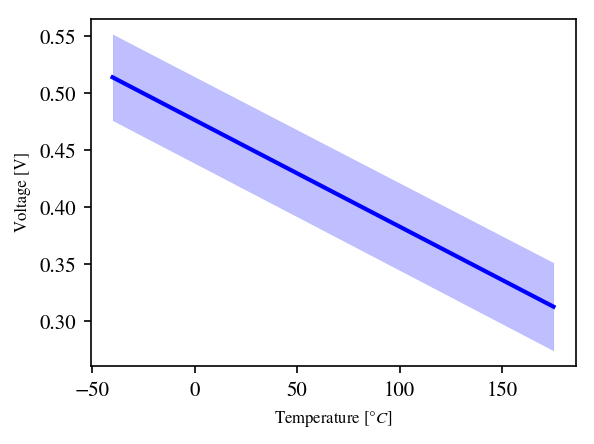
\includegraphics[width=\textwidth]{vth_nel}
		\resizebox {\textwidth} {!} {
			%% Creator: Matplotlib, PGF backend
%%
%% To include the figure in your LaTeX document, write
%%   \input{<filename>.pgf}
%%
%% Make sure the required packages are loaded in your preamble
%%   \usepackage{pgf}
%%
%% Figures using additional raster images can only be included by \input if
%% they are in the same directory as the main LaTeX file. For loading figures
%% from other directories you can use the `import` package
%%   \usepackage{import}
%% and then include the figures with
%%   \import{<path to file>}{<filename>.pgf}
%%
%% Matplotlib used the following preamble
%%   \usepackage{gensymb}
%%   \usepackage[utf8x]{inputenc}
%%   \usepackage[T1]{fontenc}
%%
\begingroup%
\makeatletter%
\begin{pgfpicture}%
\pgfpathrectangle{\pgfpointorigin}{\pgfqpoint{3.840000in}{2.840000in}}%
\pgfusepath{use as bounding box, clip}%
\begin{pgfscope}%
\pgfsetbuttcap%
\pgfsetmiterjoin%
\definecolor{currentfill}{rgb}{1.000000,1.000000,1.000000}%
\pgfsetfillcolor{currentfill}%
\pgfsetlinewidth{0.000000pt}%
\definecolor{currentstroke}{rgb}{1.000000,1.000000,1.000000}%
\pgfsetstrokecolor{currentstroke}%
\pgfsetdash{}{0pt}%
\pgfpathmoveto{\pgfqpoint{0.000000in}{0.000000in}}%
\pgfpathlineto{\pgfqpoint{3.840000in}{0.000000in}}%
\pgfpathlineto{\pgfqpoint{3.840000in}{2.840000in}}%
\pgfpathlineto{\pgfqpoint{0.000000in}{2.840000in}}%
\pgfpathclose%
\pgfusepath{fill}%
\end{pgfscope}%
\begin{pgfscope}%
\pgfsetbuttcap%
\pgfsetmiterjoin%
\definecolor{currentfill}{rgb}{1.000000,1.000000,1.000000}%
\pgfsetfillcolor{currentfill}%
\pgfsetlinewidth{0.000000pt}%
\definecolor{currentstroke}{rgb}{0.000000,0.000000,0.000000}%
\pgfsetstrokecolor{currentstroke}%
\pgfsetstrokeopacity{0.000000}%
\pgfsetdash{}{0pt}%
\pgfpathmoveto{\pgfqpoint{0.669632in}{0.596026in}}%
\pgfpathlineto{\pgfqpoint{3.716667in}{0.596026in}}%
\pgfpathlineto{\pgfqpoint{3.716667in}{2.716667in}}%
\pgfpathlineto{\pgfqpoint{0.669632in}{2.716667in}}%
\pgfpathclose%
\pgfusepath{fill}%
\end{pgfscope}%
\begin{pgfscope}%
\pgfpathrectangle{\pgfqpoint{0.669632in}{0.596026in}}{\pgfqpoint{3.047035in}{2.120641in}} %
\pgfusepath{clip}%
\pgfsetbuttcap%
\pgfsetroundjoin%
\definecolor{currentfill}{rgb}{0.000000,0.000000,1.000000}%
\pgfsetfillcolor{currentfill}%
\pgfsetfillopacity{0.250000}%
\pgfsetlinewidth{0.100375pt}%
\definecolor{currentstroke}{rgb}{0.000000,0.000000,1.000000}%
\pgfsetstrokecolor{currentstroke}%
\pgfsetstrokeopacity{0.250000}%
\pgfsetdash{}{0pt}%
\pgfpathmoveto{\pgfqpoint{0.808134in}{2.620274in}}%
\pgfpathlineto{\pgfqpoint{0.808134in}{2.096052in}}%
\pgfpathlineto{\pgfqpoint{1.001392in}{1.998114in}}%
\pgfpathlineto{\pgfqpoint{1.323488in}{1.835296in}}%
\pgfpathlineto{\pgfqpoint{1.671353in}{1.659042in}}%
\pgfpathlineto{\pgfqpoint{1.967682in}{1.508987in}}%
\pgfpathlineto{\pgfqpoint{2.289778in}{1.345787in}}%
\pgfpathlineto{\pgfqpoint{2.418617in}{1.280326in}}%
\pgfpathlineto{\pgfqpoint{2.611875in}{1.182633in}}%
\pgfpathlineto{\pgfqpoint{2.933972in}{1.019122in}}%
\pgfpathlineto{\pgfqpoint{3.256068in}{0.855719in}}%
\pgfpathlineto{\pgfqpoint{3.578165in}{0.692419in}}%
\pgfpathlineto{\pgfqpoint{3.578165in}{1.227117in}}%
\pgfpathlineto{\pgfqpoint{3.578165in}{1.227117in}}%
\pgfpathlineto{\pgfqpoint{3.256068in}{1.388933in}}%
\pgfpathlineto{\pgfqpoint{2.933972in}{1.550813in}}%
\pgfpathlineto{\pgfqpoint{2.611875in}{1.712502in}}%
\pgfpathlineto{\pgfqpoint{2.418617in}{1.809806in}}%
\pgfpathlineto{\pgfqpoint{2.289778in}{1.874491in}}%
\pgfpathlineto{\pgfqpoint{1.967682in}{2.036547in}}%
\pgfpathlineto{\pgfqpoint{1.671353in}{2.185618in}}%
\pgfpathlineto{\pgfqpoint{1.323488in}{2.360694in}}%
\pgfpathlineto{\pgfqpoint{1.001392in}{2.523020in}}%
\pgfpathlineto{\pgfqpoint{0.808134in}{2.620274in}}%
\pgfpathclose%
\pgfusepath{stroke,fill}%
\end{pgfscope}%
\begin{pgfscope}%
\pgfsetbuttcap%
\pgfsetroundjoin%
\definecolor{currentfill}{rgb}{0.000000,0.000000,0.000000}%
\pgfsetfillcolor{currentfill}%
\pgfsetlinewidth{0.803000pt}%
\definecolor{currentstroke}{rgb}{0.000000,0.000000,0.000000}%
\pgfsetstrokecolor{currentstroke}%
\pgfsetdash{}{0pt}%
\pgfsys@defobject{currentmarker}{\pgfqpoint{0.000000in}{-0.048611in}}{\pgfqpoint{0.000000in}{0.000000in}}{%
\pgfpathmoveto{\pgfqpoint{0.000000in}{0.000000in}}%
\pgfpathlineto{\pgfqpoint{0.000000in}{-0.048611in}}%
\pgfusepath{stroke,fill}%
}%
\begin{pgfscope}%
\pgfsys@transformshift{0.679295in}{0.596026in}%
\pgfsys@useobject{currentmarker}{}%
\end{pgfscope}%
\end{pgfscope}%
\begin{pgfscope}%
\pgftext[x=0.679295in,y=0.498804in,,top]{\fontsize{14.000000}{16.800000}\selectfont \(\displaystyle -50\)}%
\end{pgfscope}%
\begin{pgfscope}%
\pgfsetbuttcap%
\pgfsetroundjoin%
\definecolor{currentfill}{rgb}{0.000000,0.000000,0.000000}%
\pgfsetfillcolor{currentfill}%
\pgfsetlinewidth{0.803000pt}%
\definecolor{currentstroke}{rgb}{0.000000,0.000000,0.000000}%
\pgfsetstrokecolor{currentstroke}%
\pgfsetdash{}{0pt}%
\pgfsys@defobject{currentmarker}{\pgfqpoint{0.000000in}{-0.048611in}}{\pgfqpoint{0.000000in}{0.000000in}}{%
\pgfpathmoveto{\pgfqpoint{0.000000in}{0.000000in}}%
\pgfpathlineto{\pgfqpoint{0.000000in}{-0.048611in}}%
\pgfusepath{stroke,fill}%
}%
\begin{pgfscope}%
\pgfsys@transformshift{1.323488in}{0.596026in}%
\pgfsys@useobject{currentmarker}{}%
\end{pgfscope}%
\end{pgfscope}%
\begin{pgfscope}%
\pgftext[x=1.323488in,y=0.498804in,,top]{\fontsize{14.000000}{16.800000}\selectfont \(\displaystyle 0\)}%
\end{pgfscope}%
\begin{pgfscope}%
\pgfsetbuttcap%
\pgfsetroundjoin%
\definecolor{currentfill}{rgb}{0.000000,0.000000,0.000000}%
\pgfsetfillcolor{currentfill}%
\pgfsetlinewidth{0.803000pt}%
\definecolor{currentstroke}{rgb}{0.000000,0.000000,0.000000}%
\pgfsetstrokecolor{currentstroke}%
\pgfsetdash{}{0pt}%
\pgfsys@defobject{currentmarker}{\pgfqpoint{0.000000in}{-0.048611in}}{\pgfqpoint{0.000000in}{0.000000in}}{%
\pgfpathmoveto{\pgfqpoint{0.000000in}{0.000000in}}%
\pgfpathlineto{\pgfqpoint{0.000000in}{-0.048611in}}%
\pgfusepath{stroke,fill}%
}%
\begin{pgfscope}%
\pgfsys@transformshift{1.967682in}{0.596026in}%
\pgfsys@useobject{currentmarker}{}%
\end{pgfscope}%
\end{pgfscope}%
\begin{pgfscope}%
\pgftext[x=1.967682in,y=0.498804in,,top]{\fontsize{14.000000}{16.800000}\selectfont \(\displaystyle 50\)}%
\end{pgfscope}%
\begin{pgfscope}%
\pgfsetbuttcap%
\pgfsetroundjoin%
\definecolor{currentfill}{rgb}{0.000000,0.000000,0.000000}%
\pgfsetfillcolor{currentfill}%
\pgfsetlinewidth{0.803000pt}%
\definecolor{currentstroke}{rgb}{0.000000,0.000000,0.000000}%
\pgfsetstrokecolor{currentstroke}%
\pgfsetdash{}{0pt}%
\pgfsys@defobject{currentmarker}{\pgfqpoint{0.000000in}{-0.048611in}}{\pgfqpoint{0.000000in}{0.000000in}}{%
\pgfpathmoveto{\pgfqpoint{0.000000in}{0.000000in}}%
\pgfpathlineto{\pgfqpoint{0.000000in}{-0.048611in}}%
\pgfusepath{stroke,fill}%
}%
\begin{pgfscope}%
\pgfsys@transformshift{2.611875in}{0.596026in}%
\pgfsys@useobject{currentmarker}{}%
\end{pgfscope}%
\end{pgfscope}%
\begin{pgfscope}%
\pgftext[x=2.611875in,y=0.498804in,,top]{\fontsize{14.000000}{16.800000}\selectfont \(\displaystyle 100\)}%
\end{pgfscope}%
\begin{pgfscope}%
\pgfsetbuttcap%
\pgfsetroundjoin%
\definecolor{currentfill}{rgb}{0.000000,0.000000,0.000000}%
\pgfsetfillcolor{currentfill}%
\pgfsetlinewidth{0.803000pt}%
\definecolor{currentstroke}{rgb}{0.000000,0.000000,0.000000}%
\pgfsetstrokecolor{currentstroke}%
\pgfsetdash{}{0pt}%
\pgfsys@defobject{currentmarker}{\pgfqpoint{0.000000in}{-0.048611in}}{\pgfqpoint{0.000000in}{0.000000in}}{%
\pgfpathmoveto{\pgfqpoint{0.000000in}{0.000000in}}%
\pgfpathlineto{\pgfqpoint{0.000000in}{-0.048611in}}%
\pgfusepath{stroke,fill}%
}%
\begin{pgfscope}%
\pgfsys@transformshift{3.256068in}{0.596026in}%
\pgfsys@useobject{currentmarker}{}%
\end{pgfscope}%
\end{pgfscope}%
\begin{pgfscope}%
\pgftext[x=3.256068in,y=0.498804in,,top]{\fontsize{14.000000}{16.800000}\selectfont \(\displaystyle 150\)}%
\end{pgfscope}%
\begin{pgfscope}%
\pgftext[x=2.193149in,y=0.266626in,,top]{\fontsize{12.000000}{14.400000}\selectfont Temperature [\(\displaystyle \degree C\)]}%
\end{pgfscope}%
\begin{pgfscope}%
\pgfsetbuttcap%
\pgfsetroundjoin%
\definecolor{currentfill}{rgb}{0.000000,0.000000,0.000000}%
\pgfsetfillcolor{currentfill}%
\pgfsetlinewidth{0.803000pt}%
\definecolor{currentstroke}{rgb}{0.000000,0.000000,0.000000}%
\pgfsetstrokecolor{currentstroke}%
\pgfsetdash{}{0pt}%
\pgfsys@defobject{currentmarker}{\pgfqpoint{-0.048611in}{0.000000in}}{\pgfqpoint{0.000000in}{0.000000in}}{%
\pgfpathmoveto{\pgfqpoint{0.000000in}{0.000000in}}%
\pgfpathlineto{\pgfqpoint{-0.048611in}{0.000000in}}%
\pgfusepath{stroke,fill}%
}%
\begin{pgfscope}%
\pgfsys@transformshift{0.669632in}{0.871136in}%
\pgfsys@useobject{currentmarker}{}%
\end{pgfscope}%
\end{pgfscope}%
\begin{pgfscope}%
\pgftext[x=0.322182in,y=0.802270in,left,base]{\fontsize{14.000000}{16.800000}\selectfont \(\displaystyle 0.3\)}%
\end{pgfscope}%
\begin{pgfscope}%
\pgfsetbuttcap%
\pgfsetroundjoin%
\definecolor{currentfill}{rgb}{0.000000,0.000000,0.000000}%
\pgfsetfillcolor{currentfill}%
\pgfsetlinewidth{0.803000pt}%
\definecolor{currentstroke}{rgb}{0.000000,0.000000,0.000000}%
\pgfsetstrokecolor{currentstroke}%
\pgfsetdash{}{0pt}%
\pgfsys@defobject{currentmarker}{\pgfqpoint{-0.048611in}{0.000000in}}{\pgfqpoint{0.000000in}{0.000000in}}{%
\pgfpathmoveto{\pgfqpoint{0.000000in}{0.000000in}}%
\pgfpathlineto{\pgfqpoint{-0.048611in}{0.000000in}}%
\pgfusepath{stroke,fill}%
}%
\begin{pgfscope}%
\pgfsys@transformshift{0.669632in}{1.566067in}%
\pgfsys@useobject{currentmarker}{}%
\end{pgfscope}%
\end{pgfscope}%
\begin{pgfscope}%
\pgftext[x=0.322182in,y=1.497201in,left,base]{\fontsize{14.000000}{16.800000}\selectfont \(\displaystyle 0.4\)}%
\end{pgfscope}%
\begin{pgfscope}%
\pgfsetbuttcap%
\pgfsetroundjoin%
\definecolor{currentfill}{rgb}{0.000000,0.000000,0.000000}%
\pgfsetfillcolor{currentfill}%
\pgfsetlinewidth{0.803000pt}%
\definecolor{currentstroke}{rgb}{0.000000,0.000000,0.000000}%
\pgfsetstrokecolor{currentstroke}%
\pgfsetdash{}{0pt}%
\pgfsys@defobject{currentmarker}{\pgfqpoint{-0.048611in}{0.000000in}}{\pgfqpoint{0.000000in}{0.000000in}}{%
\pgfpathmoveto{\pgfqpoint{0.000000in}{0.000000in}}%
\pgfpathlineto{\pgfqpoint{-0.048611in}{0.000000in}}%
\pgfusepath{stroke,fill}%
}%
\begin{pgfscope}%
\pgfsys@transformshift{0.669632in}{2.260998in}%
\pgfsys@useobject{currentmarker}{}%
\end{pgfscope}%
\end{pgfscope}%
\begin{pgfscope}%
\pgftext[x=0.322182in,y=2.192132in,left,base]{\fontsize{14.000000}{16.800000}\selectfont \(\displaystyle 0.5\)}%
\end{pgfscope}%
\begin{pgfscope}%
\pgftext[x=0.266626in,y=1.656346in,,bottom,rotate=90.000000]{\fontsize{12.000000}{14.400000}\selectfont Voltage [V]}%
\end{pgfscope}%
\begin{pgfscope}%
\pgfpathrectangle{\pgfqpoint{0.669632in}{0.596026in}}{\pgfqpoint{3.047035in}{2.120641in}} %
\pgfusepath{clip}%
\pgfsetrectcap%
\pgfsetroundjoin%
\pgfsetlinewidth{2.007500pt}%
\definecolor{currentstroke}{rgb}{0.000000,0.000000,1.000000}%
\pgfsetstrokecolor{currentstroke}%
\pgfsetdash{}{0pt}%
\pgfpathmoveto{\pgfqpoint{0.808134in}{2.358163in}}%
\pgfpathlineto{\pgfqpoint{1.001392in}{2.260567in}}%
\pgfpathlineto{\pgfqpoint{1.323488in}{2.097995in}}%
\pgfpathlineto{\pgfqpoint{1.671353in}{1.922330in}}%
\pgfpathlineto{\pgfqpoint{1.967682in}{1.772767in}}%
\pgfpathlineto{\pgfqpoint{2.289778in}{1.610139in}}%
\pgfpathlineto{\pgfqpoint{2.418617in}{1.545066in}}%
\pgfpathlineto{\pgfqpoint{2.611875in}{1.447567in}}%
\pgfpathlineto{\pgfqpoint{2.933972in}{1.284967in}}%
\pgfpathlineto{\pgfqpoint{3.256068in}{1.122326in}}%
\pgfpathlineto{\pgfqpoint{3.578165in}{0.959768in}}%
\pgfusepath{stroke}%
\end{pgfscope}%
\begin{pgfscope}%
\pgfsetrectcap%
\pgfsetmiterjoin%
\pgfsetlinewidth{0.803000pt}%
\definecolor{currentstroke}{rgb}{0.000000,0.000000,0.000000}%
\pgfsetstrokecolor{currentstroke}%
\pgfsetdash{}{0pt}%
\pgfpathmoveto{\pgfqpoint{0.669632in}{0.596026in}}%
\pgfpathlineto{\pgfqpoint{0.669632in}{2.716667in}}%
\pgfusepath{stroke}%
\end{pgfscope}%
\begin{pgfscope}%
\pgfsetrectcap%
\pgfsetmiterjoin%
\pgfsetlinewidth{0.803000pt}%
\definecolor{currentstroke}{rgb}{0.000000,0.000000,0.000000}%
\pgfsetstrokecolor{currentstroke}%
\pgfsetdash{}{0pt}%
\pgfpathmoveto{\pgfqpoint{3.716667in}{0.596026in}}%
\pgfpathlineto{\pgfqpoint{3.716667in}{2.716667in}}%
\pgfusepath{stroke}%
\end{pgfscope}%
\begin{pgfscope}%
\pgfsetrectcap%
\pgfsetmiterjoin%
\pgfsetlinewidth{0.803000pt}%
\definecolor{currentstroke}{rgb}{0.000000,0.000000,0.000000}%
\pgfsetstrokecolor{currentstroke}%
\pgfsetdash{}{0pt}%
\pgfpathmoveto{\pgfqpoint{0.669632in}{0.596026in}}%
\pgfpathlineto{\pgfqpoint{3.716667in}{0.596026in}}%
\pgfusepath{stroke}%
\end{pgfscope}%
\begin{pgfscope}%
\pgfsetrectcap%
\pgfsetmiterjoin%
\pgfsetlinewidth{0.803000pt}%
\definecolor{currentstroke}{rgb}{0.000000,0.000000,0.000000}%
\pgfsetstrokecolor{currentstroke}%
\pgfsetdash{}{0pt}%
\pgfpathmoveto{\pgfqpoint{0.669632in}{2.716667in}}%
\pgfpathlineto{\pgfqpoint{3.716667in}{2.716667in}}%
\pgfusepath{stroke}%
\end{pgfscope}%
\end{pgfpicture}%
\makeatother%
\endgroup%

		}
		\subcaption{Average and \(\pm 3\sigma \) process variation range}
	\end{subfigure}
	\begin{subfigure}[b]{0.48\textwidth}
		%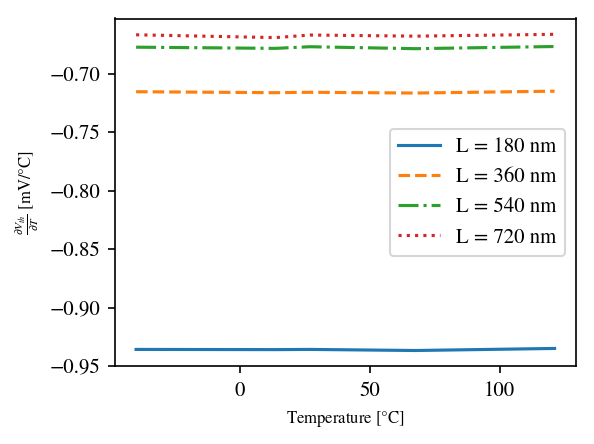
\includegraphics[width=\textwidth]{vth_nel_T}
		\resizebox {\textwidth} {!} {
			%% Creator: Matplotlib, PGF backend
%%
%% To include the figure in your LaTeX document, write
%%   \input{<filename>.pgf}
%%
%% Make sure the required packages are loaded in your preamble
%%   \usepackage{pgf}
%%
%% Figures using additional raster images can only be included by \input if
%% they are in the same directory as the main LaTeX file. For loading figures
%% from other directories you can use the `import` package
%%   \usepackage{import}
%% and then include the figures with
%%   \import{<path to file>}{<filename>.pgf}
%%
%% Matplotlib used the following preamble
%%   \usepackage{gensymb}
%%   \usepackage[utf8x]{inputenc}
%%   \usepackage[T1]{fontenc}
%%
\begingroup%
\makeatletter%
\begin{pgfpicture}%
\pgfpathrectangle{\pgfpointorigin}{\pgfqpoint{3.840000in}{2.840000in}}%
\pgfusepath{use as bounding box, clip}%
\begin{pgfscope}%
\pgfsetbuttcap%
\pgfsetmiterjoin%
\definecolor{currentfill}{rgb}{1.000000,1.000000,1.000000}%
\pgfsetfillcolor{currentfill}%
\pgfsetlinewidth{0.000000pt}%
\definecolor{currentstroke}{rgb}{1.000000,1.000000,1.000000}%
\pgfsetstrokecolor{currentstroke}%
\pgfsetdash{}{0pt}%
\pgfpathmoveto{\pgfqpoint{0.000000in}{0.000000in}}%
\pgfpathlineto{\pgfqpoint{3.840000in}{0.000000in}}%
\pgfpathlineto{\pgfqpoint{3.840000in}{2.840000in}}%
\pgfpathlineto{\pgfqpoint{0.000000in}{2.840000in}}%
\pgfpathclose%
\pgfusepath{fill}%
\end{pgfscope}%
\begin{pgfscope}%
\pgfsetbuttcap%
\pgfsetmiterjoin%
\definecolor{currentfill}{rgb}{1.000000,1.000000,1.000000}%
\pgfsetfillcolor{currentfill}%
\pgfsetlinewidth{0.000000pt}%
\definecolor{currentstroke}{rgb}{0.000000,0.000000,0.000000}%
\pgfsetstrokecolor{currentstroke}%
\pgfsetstrokeopacity{0.000000}%
\pgfsetdash{}{0pt}%
\pgfpathmoveto{\pgfqpoint{1.001379in}{0.596026in}}%
\pgfpathlineto{\pgfqpoint{3.716667in}{0.596026in}}%
\pgfpathlineto{\pgfqpoint{3.716667in}{2.716667in}}%
\pgfpathlineto{\pgfqpoint{1.001379in}{2.716667in}}%
\pgfpathclose%
\pgfusepath{fill}%
\end{pgfscope}%
\begin{pgfscope}%
\pgfsetbuttcap%
\pgfsetroundjoin%
\definecolor{currentfill}{rgb}{0.000000,0.000000,0.000000}%
\pgfsetfillcolor{currentfill}%
\pgfsetlinewidth{0.803000pt}%
\definecolor{currentstroke}{rgb}{0.000000,0.000000,0.000000}%
\pgfsetstrokecolor{currentstroke}%
\pgfsetdash{}{0pt}%
\pgfsys@defobject{currentmarker}{\pgfqpoint{0.000000in}{-0.048611in}}{\pgfqpoint{0.000000in}{0.000000in}}{%
\pgfpathmoveto{\pgfqpoint{0.000000in}{0.000000in}}%
\pgfpathlineto{\pgfqpoint{0.000000in}{-0.048611in}}%
\pgfusepath{stroke,fill}%
}%
\begin{pgfscope}%
\pgfsys@transformshift{1.737318in}{0.596026in}%
\pgfsys@useobject{currentmarker}{}%
\end{pgfscope}%
\end{pgfscope}%
\begin{pgfscope}%
\pgftext[x=1.737318in,y=0.498804in,,top]{\fontsize{14.000000}{16.800000}\selectfont \(\displaystyle 0\)}%
\end{pgfscope}%
\begin{pgfscope}%
\pgfsetbuttcap%
\pgfsetroundjoin%
\definecolor{currentfill}{rgb}{0.000000,0.000000,0.000000}%
\pgfsetfillcolor{currentfill}%
\pgfsetlinewidth{0.803000pt}%
\definecolor{currentstroke}{rgb}{0.000000,0.000000,0.000000}%
\pgfsetstrokecolor{currentstroke}%
\pgfsetdash{}{0pt}%
\pgfsys@defobject{currentmarker}{\pgfqpoint{0.000000in}{-0.048611in}}{\pgfqpoint{0.000000in}{0.000000in}}{%
\pgfpathmoveto{\pgfqpoint{0.000000in}{0.000000in}}%
\pgfpathlineto{\pgfqpoint{0.000000in}{-0.048611in}}%
\pgfusepath{stroke,fill}%
}%
\begin{pgfscope}%
\pgfsys@transformshift{2.502964in}{0.596026in}%
\pgfsys@useobject{currentmarker}{}%
\end{pgfscope}%
\end{pgfscope}%
\begin{pgfscope}%
\pgftext[x=2.502964in,y=0.498804in,,top]{\fontsize{14.000000}{16.800000}\selectfont \(\displaystyle 50\)}%
\end{pgfscope}%
\begin{pgfscope}%
\pgfsetbuttcap%
\pgfsetroundjoin%
\definecolor{currentfill}{rgb}{0.000000,0.000000,0.000000}%
\pgfsetfillcolor{currentfill}%
\pgfsetlinewidth{0.803000pt}%
\definecolor{currentstroke}{rgb}{0.000000,0.000000,0.000000}%
\pgfsetstrokecolor{currentstroke}%
\pgfsetdash{}{0pt}%
\pgfsys@defobject{currentmarker}{\pgfqpoint{0.000000in}{-0.048611in}}{\pgfqpoint{0.000000in}{0.000000in}}{%
\pgfpathmoveto{\pgfqpoint{0.000000in}{0.000000in}}%
\pgfpathlineto{\pgfqpoint{0.000000in}{-0.048611in}}%
\pgfusepath{stroke,fill}%
}%
\begin{pgfscope}%
\pgfsys@transformshift{3.268610in}{0.596026in}%
\pgfsys@useobject{currentmarker}{}%
\end{pgfscope}%
\end{pgfscope}%
\begin{pgfscope}%
\pgftext[x=3.268610in,y=0.498804in,,top]{\fontsize{14.000000}{16.800000}\selectfont \(\displaystyle 100\)}%
\end{pgfscope}%
\begin{pgfscope}%
\pgftext[x=2.359023in,y=0.266626in,,top]{\fontsize{12.000000}{14.400000}\selectfont Temperature [\(\displaystyle \degree\)C]}%
\end{pgfscope}%
\begin{pgfscope}%
\pgfsetbuttcap%
\pgfsetroundjoin%
\definecolor{currentfill}{rgb}{0.000000,0.000000,0.000000}%
\pgfsetfillcolor{currentfill}%
\pgfsetlinewidth{0.803000pt}%
\definecolor{currentstroke}{rgb}{0.000000,0.000000,0.000000}%
\pgfsetstrokecolor{currentstroke}%
\pgfsetdash{}{0pt}%
\pgfsys@defobject{currentmarker}{\pgfqpoint{-0.048611in}{0.000000in}}{\pgfqpoint{0.000000in}{0.000000in}}{%
\pgfpathmoveto{\pgfqpoint{0.000000in}{0.000000in}}%
\pgfpathlineto{\pgfqpoint{-0.048611in}{0.000000in}}%
\pgfusepath{stroke,fill}%
}%
\begin{pgfscope}%
\pgfsys@transformshift{1.001379in}{0.954608in}%
\pgfsys@useobject{currentmarker}{}%
\end{pgfscope}%
\end{pgfscope}%
\begin{pgfscope}%
\pgftext[x=0.498372in,y=0.885742in,left,base]{\fontsize{14.000000}{16.800000}\selectfont \(\displaystyle -0.9\)}%
\end{pgfscope}%
\begin{pgfscope}%
\pgfsetbuttcap%
\pgfsetroundjoin%
\definecolor{currentfill}{rgb}{0.000000,0.000000,0.000000}%
\pgfsetfillcolor{currentfill}%
\pgfsetlinewidth{0.803000pt}%
\definecolor{currentstroke}{rgb}{0.000000,0.000000,0.000000}%
\pgfsetstrokecolor{currentstroke}%
\pgfsetdash{}{0pt}%
\pgfsys@defobject{currentmarker}{\pgfqpoint{-0.048611in}{0.000000in}}{\pgfqpoint{0.000000in}{0.000000in}}{%
\pgfpathmoveto{\pgfqpoint{0.000000in}{0.000000in}}%
\pgfpathlineto{\pgfqpoint{-0.048611in}{0.000000in}}%
\pgfusepath{stroke,fill}%
}%
\begin{pgfscope}%
\pgfsys@transformshift{1.001379in}{1.667859in}%
\pgfsys@useobject{currentmarker}{}%
\end{pgfscope}%
\end{pgfscope}%
\begin{pgfscope}%
\pgftext[x=0.498372in,y=1.598993in,left,base]{\fontsize{14.000000}{16.800000}\selectfont \(\displaystyle -0.8\)}%
\end{pgfscope}%
\begin{pgfscope}%
\pgfsetbuttcap%
\pgfsetroundjoin%
\definecolor{currentfill}{rgb}{0.000000,0.000000,0.000000}%
\pgfsetfillcolor{currentfill}%
\pgfsetlinewidth{0.803000pt}%
\definecolor{currentstroke}{rgb}{0.000000,0.000000,0.000000}%
\pgfsetstrokecolor{currentstroke}%
\pgfsetdash{}{0pt}%
\pgfsys@defobject{currentmarker}{\pgfqpoint{-0.048611in}{0.000000in}}{\pgfqpoint{0.000000in}{0.000000in}}{%
\pgfpathmoveto{\pgfqpoint{0.000000in}{0.000000in}}%
\pgfpathlineto{\pgfqpoint{-0.048611in}{0.000000in}}%
\pgfusepath{stroke,fill}%
}%
\begin{pgfscope}%
\pgfsys@transformshift{1.001379in}{2.381110in}%
\pgfsys@useobject{currentmarker}{}%
\end{pgfscope}%
\end{pgfscope}%
\begin{pgfscope}%
\pgftext[x=0.498372in,y=2.312243in,left,base]{\fontsize{14.000000}{16.800000}\selectfont \(\displaystyle -0.7\)}%
\end{pgfscope}%
\begin{pgfscope}%
\pgftext[x=0.442817in,y=1.656346in,,bottom,rotate=90.000000]{\fontsize{12.000000}{14.400000}\selectfont \(\displaystyle \frac{\partial V_{th}}{\partial T}\) [mV/\(\displaystyle \degree\)C]}%
\end{pgfscope}%
\begin{pgfscope}%
\pgfpathrectangle{\pgfqpoint{1.001379in}{0.596026in}}{\pgfqpoint{2.715288in}{2.120641in}} %
\pgfusepath{clip}%
\pgfsetrectcap%
\pgfsetroundjoin%
\pgfsetlinewidth{1.505625pt}%
\definecolor{currentstroke}{rgb}{0.121569,0.466667,0.705882}%
\pgfsetstrokecolor{currentstroke}%
\pgfsetdash{}{0pt}%
\pgfpathmoveto{\pgfqpoint{1.124801in}{0.699032in}}%
\pgfpathlineto{\pgfqpoint{1.947871in}{0.697838in}}%
\pgfpathlineto{\pgfqpoint{2.150767in}{0.699071in}}%
\pgfpathlineto{\pgfqpoint{2.770940in}{0.692419in}}%
\pgfpathlineto{\pgfqpoint{3.593244in}{0.704970in}}%
\pgfusepath{stroke}%
\end{pgfscope}%
\begin{pgfscope}%
\pgfpathrectangle{\pgfqpoint{1.001379in}{0.596026in}}{\pgfqpoint{2.715288in}{2.120641in}} %
\pgfusepath{clip}%
\pgfsetbuttcap%
\pgfsetroundjoin%
\pgfsetlinewidth{1.505625pt}%
\definecolor{currentstroke}{rgb}{1.000000,0.498039,0.054902}%
\pgfsetstrokecolor{currentstroke}%
\pgfsetdash{{5.550000pt}{2.400000pt}}{0.000000pt}%
\pgfpathmoveto{\pgfqpoint{1.124801in}{2.270307in}}%
\pgfpathlineto{\pgfqpoint{1.947871in}{2.264298in}}%
\pgfpathlineto{\pgfqpoint{2.150767in}{2.266813in}}%
\pgfpathlineto{\pgfqpoint{2.770940in}{2.262102in}}%
\pgfpathlineto{\pgfqpoint{3.593244in}{2.273592in}}%
\pgfusepath{stroke}%
\end{pgfscope}%
\begin{pgfscope}%
\pgfpathrectangle{\pgfqpoint{1.001379in}{0.596026in}}{\pgfqpoint{2.715288in}{2.120641in}} %
\pgfusepath{clip}%
\pgfsetbuttcap%
\pgfsetroundjoin%
\pgfsetlinewidth{1.505625pt}%
\definecolor{currentstroke}{rgb}{0.172549,0.627451,0.172549}%
\pgfsetstrokecolor{currentstroke}%
\pgfsetdash{{9.600000pt}{2.400000pt}{1.500000pt}{2.400000pt}}{0.000000pt}%
\pgfpathmoveto{\pgfqpoint{1.124801in}{2.541807in}}%
\pgfpathlineto{\pgfqpoint{1.947871in}{2.534526in}}%
\pgfpathlineto{\pgfqpoint{2.150767in}{2.544541in}}%
\pgfpathlineto{\pgfqpoint{2.770940in}{2.532659in}}%
\pgfpathlineto{\pgfqpoint{3.593244in}{2.545900in}}%
\pgfusepath{stroke}%
\end{pgfscope}%
\begin{pgfscope}%
\pgfpathrectangle{\pgfqpoint{1.001379in}{0.596026in}}{\pgfqpoint{2.715288in}{2.120641in}} %
\pgfusepath{clip}%
\pgfsetbuttcap%
\pgfsetroundjoin%
\pgfsetlinewidth{1.505625pt}%
\definecolor{currentstroke}{rgb}{0.839216,0.152941,0.156863}%
\pgfsetstrokecolor{currentstroke}%
\pgfsetdash{{1.500000pt}{2.475000pt}}{0.000000pt}%
\pgfpathmoveto{\pgfqpoint{1.124801in}{2.617312in}}%
\pgfpathlineto{\pgfqpoint{1.947871in}{2.600199in}}%
\pgfpathlineto{\pgfqpoint{2.150767in}{2.615866in}}%
\pgfpathlineto{\pgfqpoint{2.770940in}{2.609031in}}%
\pgfpathlineto{\pgfqpoint{3.593244in}{2.620274in}}%
\pgfusepath{stroke}%
\end{pgfscope}%
\begin{pgfscope}%
\pgfsetrectcap%
\pgfsetmiterjoin%
\pgfsetlinewidth{0.803000pt}%
\definecolor{currentstroke}{rgb}{0.000000,0.000000,0.000000}%
\pgfsetstrokecolor{currentstroke}%
\pgfsetdash{}{0pt}%
\pgfpathmoveto{\pgfqpoint{1.001379in}{0.596026in}}%
\pgfpathlineto{\pgfqpoint{1.001379in}{2.716667in}}%
\pgfusepath{stroke}%
\end{pgfscope}%
\begin{pgfscope}%
\pgfsetrectcap%
\pgfsetmiterjoin%
\pgfsetlinewidth{0.803000pt}%
\definecolor{currentstroke}{rgb}{0.000000,0.000000,0.000000}%
\pgfsetstrokecolor{currentstroke}%
\pgfsetdash{}{0pt}%
\pgfpathmoveto{\pgfqpoint{3.716667in}{0.596026in}}%
\pgfpathlineto{\pgfqpoint{3.716667in}{2.716667in}}%
\pgfusepath{stroke}%
\end{pgfscope}%
\begin{pgfscope}%
\pgfsetrectcap%
\pgfsetmiterjoin%
\pgfsetlinewidth{0.803000pt}%
\definecolor{currentstroke}{rgb}{0.000000,0.000000,0.000000}%
\pgfsetstrokecolor{currentstroke}%
\pgfsetdash{}{0pt}%
\pgfpathmoveto{\pgfqpoint{1.001379in}{0.596026in}}%
\pgfpathlineto{\pgfqpoint{3.716667in}{0.596026in}}%
\pgfusepath{stroke}%
\end{pgfscope}%
\begin{pgfscope}%
\pgfsetrectcap%
\pgfsetmiterjoin%
\pgfsetlinewidth{0.803000pt}%
\definecolor{currentstroke}{rgb}{0.000000,0.000000,0.000000}%
\pgfsetstrokecolor{currentstroke}%
\pgfsetdash{}{0pt}%
\pgfpathmoveto{\pgfqpoint{1.001379in}{2.716667in}}%
\pgfpathlineto{\pgfqpoint{3.716667in}{2.716667in}}%
\pgfusepath{stroke}%
\end{pgfscope}%
\begin{pgfscope}%
\pgfsetbuttcap%
\pgfsetmiterjoin%
\definecolor{currentfill}{rgb}{1.000000,1.000000,1.000000}%
\pgfsetfillcolor{currentfill}%
\pgfsetfillopacity{0.800000}%
\pgfsetlinewidth{1.003750pt}%
\definecolor{currentstroke}{rgb}{0.800000,0.800000,0.800000}%
\pgfsetstrokecolor{currentstroke}%
\pgfsetstrokeopacity{0.800000}%
\pgfsetdash{}{0pt}%
\pgfpathmoveto{\pgfqpoint{1.950894in}{1.079491in}}%
\pgfpathlineto{\pgfqpoint{3.580556in}{1.079491in}}%
\pgfpathquadraticcurveto{\pgfqpoint{3.619444in}{1.079491in}}{\pgfqpoint{3.619444in}{1.118380in}}%
\pgfpathlineto{\pgfqpoint{3.619444in}{2.194313in}}%
\pgfpathquadraticcurveto{\pgfqpoint{3.619444in}{2.233202in}}{\pgfqpoint{3.580556in}{2.233202in}}%
\pgfpathlineto{\pgfqpoint{1.950894in}{2.233202in}}%
\pgfpathquadraticcurveto{\pgfqpoint{1.912005in}{2.233202in}}{\pgfqpoint{1.912005in}{2.194313in}}%
\pgfpathlineto{\pgfqpoint{1.912005in}{1.118380in}}%
\pgfpathquadraticcurveto{\pgfqpoint{1.912005in}{1.079491in}}{\pgfqpoint{1.950894in}{1.079491in}}%
\pgfpathclose%
\pgfusepath{stroke,fill}%
\end{pgfscope}%
\begin{pgfscope}%
\pgfsetrectcap%
\pgfsetroundjoin%
\pgfsetlinewidth{1.505625pt}%
\definecolor{currentstroke}{rgb}{0.121569,0.466667,0.705882}%
\pgfsetstrokecolor{currentstroke}%
\pgfsetdash{}{0pt}%
\pgfpathmoveto{\pgfqpoint{1.989783in}{2.085747in}}%
\pgfpathlineto{\pgfqpoint{2.378672in}{2.085747in}}%
\pgfusepath{stroke}%
\end{pgfscope}%
\begin{pgfscope}%
\pgftext[x=2.534227in,y=2.017692in,left,base]{\fontsize{14.000000}{16.800000}\selectfont L = 180 nm}%
\end{pgfscope}%
\begin{pgfscope}%
\pgfsetbuttcap%
\pgfsetroundjoin%
\pgfsetlinewidth{1.505625pt}%
\definecolor{currentstroke}{rgb}{1.000000,0.498039,0.054902}%
\pgfsetstrokecolor{currentstroke}%
\pgfsetdash{{5.550000pt}{2.400000pt}}{0.000000pt}%
\pgfpathmoveto{\pgfqpoint{1.989783in}{1.811903in}}%
\pgfpathlineto{\pgfqpoint{2.378672in}{1.811903in}}%
\pgfusepath{stroke}%
\end{pgfscope}%
\begin{pgfscope}%
\pgftext[x=2.534227in,y=1.743847in,left,base]{\fontsize{14.000000}{16.800000}\selectfont L = 360 nm}%
\end{pgfscope}%
\begin{pgfscope}%
\pgfsetbuttcap%
\pgfsetroundjoin%
\pgfsetlinewidth{1.505625pt}%
\definecolor{currentstroke}{rgb}{0.172549,0.627451,0.172549}%
\pgfsetstrokecolor{currentstroke}%
\pgfsetdash{{9.600000pt}{2.400000pt}{1.500000pt}{2.400000pt}}{0.000000pt}%
\pgfpathmoveto{\pgfqpoint{1.989783in}{1.538059in}}%
\pgfpathlineto{\pgfqpoint{2.378672in}{1.538059in}}%
\pgfusepath{stroke}%
\end{pgfscope}%
\begin{pgfscope}%
\pgftext[x=2.534227in,y=1.470003in,left,base]{\fontsize{14.000000}{16.800000}\selectfont L = 540 nm}%
\end{pgfscope}%
\begin{pgfscope}%
\pgfsetbuttcap%
\pgfsetroundjoin%
\pgfsetlinewidth{1.505625pt}%
\definecolor{currentstroke}{rgb}{0.839216,0.152941,0.156863}%
\pgfsetstrokecolor{currentstroke}%
\pgfsetdash{{1.500000pt}{2.475000pt}}{0.000000pt}%
\pgfpathmoveto{\pgfqpoint{1.989783in}{1.264214in}}%
\pgfpathlineto{\pgfqpoint{2.378672in}{1.264214in}}%
\pgfusepath{stroke}%
\end{pgfscope}%
\begin{pgfscope}%
\pgftext[x=2.534227in,y=1.196159in,left,base]{\fontsize{14.000000}{16.800000}\selectfont L = 720 nm}%
\end{pgfscope}%
\end{pgfpicture}%
\makeatother%
\endgroup%

		}
		\subcaption{Channel length effect}
		\label{fig:vth_nel_L}
	\end{subfigure}
	\caption{Threshold voltage of low-VT nMOSFET of 1\(\mu \)m/180nm over temperature under process and channel length variations}
	\label{fig:vth_nel}
\end{figure}

The slope depends on the transistor channel length L and the bulk-source voltage applied. For a voltage \(V_{bs} = 0 \) as done in the \figurename~\ref{fig:vth_nel_L}, the bigger the channel length is, the less sensitive is the threshold voltage. This offer the possibility to the designer to adjust the sensitivity of the threshold voltage to temperature by either decreasing the transistor channel length or by body biasing~\cite{Kumar2008}.


\subsubsection{Leakage Current}        % section 2.7
In semiconductor devices, leakage is a quantum phenomenon where mobile charge carriers tunnel through an insulating region. It also comes from the free charges displacement in a region subjected to an electric field. These leakages are represented in \figurename~\ref{fig:soi-mos-leakage} for an NMOS and PMOS transistor with a partially depleted SOI technology.

\begin{figure}[htp]
	\centering
	\begin{subfigure}[b]{0.48\textwidth}
		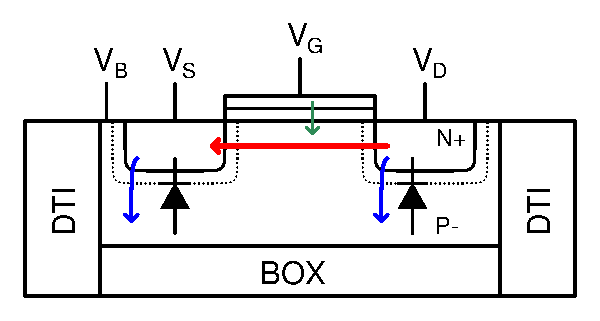
\includegraphics[width=\textwidth]{Chapter2/Figs/Vector/soi-nmos-leakage.ps}
		\caption{NMOS}
	\end{subfigure}
	\begin{subfigure}[b]{0.48\textwidth}
		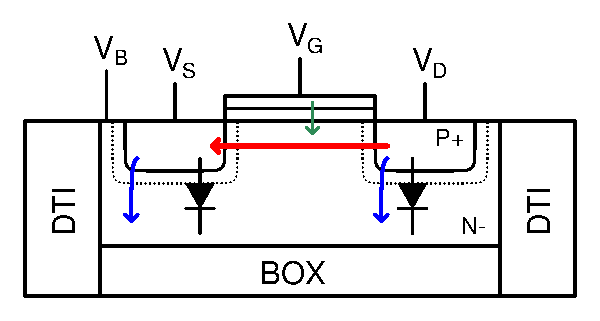
\includegraphics[width=\textwidth]{Chapter2/Figs/Vector/soi-pmos-leakage.ps}
		\caption{PMOS}
	\end{subfigure}
	\caption{Substrate leakage current in SOI transistors}
	\label{fig:soi-mos-leakage}
\end{figure}

The \textcolor{red}{off-state current} of a transistor gradually became a limiting factor for down-scaling the threshold voltage since it determines the power consumption of a chip in its idle state. In a CMOS cell at high temperature, these off-state currents of NMOS transistor are pump from the useful current of PMOS transistor. It could not be ignored longer and new physical models had to be applied to correctly describe the device behavior in the so-called sub-threshold or weak-inversion regime~\cite{Cheng21997,Enz1995,Joardar1998}. This weak-inversion current contributes as:
\begin{equation}
\label{eqn:ids_leakage}
I_{ds}(V_{gs}, V_{bs}, V_{ds}, T) = \mu_{eff} C_{ox} \frac{W}{L} {\left(\frac{k_B T}{q}\right)}^2 [n(V_{bs})-1] e^{q(V_{gs}-V_{th})/nk_B T} \left(1-e^{-qV_{ds}/k_B T} \right)
\end{equation}
where n is the slope factor, \(\mu_{eff} \) the mobility of carriers as given in Section~\ref{sec:mobility}. The leakage current due to the off state of a transistor is, therefore, increasing exponentially with the temperature. This is arguably the most challenging constraint on high-temperature design.

In addition to that, and without considering contact losses and recombination, charges also diffuse in the substrate. This \textcolor{blue}{substrate-current} depends on the electric field imposed by the MOSFET use case. In the case of an NMOS transistor as in \figurename~\ref{fig:soi-mos-leakage}a, the leakage current flow is either in one of the following configurations:
\begin{itemize}
	\item[--] $V_{\rm B} = V_{\rm S} < V_{\rm D}$: no charges flow in the intrinsic pn junction at the source but a reverse leakage current exists in the pn-junction at the drain.
	\item[--] $V_{\rm S} < V_{\rm B} < V_{\rm D}$: the reverse current in the pn-junction at the drain is smaller, and a forward leakage current occurs in the pn-junction at the source.
	\item[--] $V_{\rm S} < V_{\rm D} < V_{\rm B}$: both pn-junction at the source and at the drain are forward biased. The current flows from the bulk to each contact.
\end{itemize}

while for the PMOS transistor,
\begin{itemize}
	\item[--] $V_{\rm B} = V_{\rm S} < V_{\rm D}$: no charges flow in the intrinsic pn junction at the source but a forward leakage current exists in the pn-junction at the drain.
	\item[--] $V_{\rm S} < V_{\rm B} < V_{\rm D}$: the reverse current in the pn-junction at the source increases, and a forward leakage current occurs in the pn-junction at the drain decrease.
	\item[--] $V_{\rm S} < V_{\rm D} < V_{\rm B}$: both pn-junction at the source and at the drain are reverse biased. The current flows from each contact to the bulk.
\end{itemize}

Based on the Shockley equation, the forward and reverse current of the diode is defined by equation~(\ref{eqn:shockley-diode-leakage}) where $L_n (L_p)$ represents the equivalent height of the n-block (p-block), while $D_n (D_p)$ is the diffusion coefficients of this block, and $n_i$ is the intrinsic carrier concentration.
\begin{equation}
\label{eqn:shockley-diode-leakage}
I_{\rm db/sb} = q\left(\frac{D_n}{L_n}\frac{n_i^2}{N_a}+\frac{D_p}{L_p}\frac{n_i^2}{N_d}\right) \exp\left(\frac{qV_{\rm db/sb}}{k_BT} - 1\right)
\end{equation}

\subsection{\(g_m/I_{D} \)-based design over temperature} % section 2.8
\label{sec:analog-insight}
Physical design for analog ICs has not been automated at the same degree as digital IC design. However, computer-aided-design (CAD) can significantly improve the productivity of circuit engineers. As presented in the Section~\ref{sec:threshold}, the threshold voltage decreases with the temperature. Thus, a design methodology based on the voltage overdrive ($V_{ov} = V_{GS}-V_{th}$) will be difficult and time-consuming. To the contrary, the \(g_m/I_{D} \) methodology employs design charts to accurately size transistors which fits well the purpose of productivity. Moreover, a \(g_m/I_{D} \)-based design methodology links design variables (\(g_m \), \(f_T \), \(I_d \), \ldots) to analog macro blocks specification such as the bandwidth, the power consumption, the noise budget, or accuracy.
\nomenclature[A-gm]{$g_m$}{transistor small signal transconductance}
\nomenclature[A-Z]{CAD}{computer-aided-design}

The analysis of the variations of each circuit's characteristics, as noise figure, gain, bandwidth or power consumption, as function the \(g_m/I_{D} \) parameter over temperature helps us to select the MOS transistor optimum inversion region to have a design cost equilibrated to the temperature related design~\cite{Silveira1996,Ou2014,Ou2017,Ou2018}.

\subsubsection{High-Frequency design over temperature}
\label{sec:des_speed}
In the design of high-speed integrated circuits, PLL and RF-Amplifiers are few applications among many using transistors at the limit of their speed with an important criterion on the in-band noise. Usually with a low-impedance and at the largest transconductance possible, a transistor acts as a current source or current sink to either charge or discharge the capacitive load. In such circumstances, a very high frequency signal encounters a primary limitation known as slew rate, i.e. a limited speed as long as a transistor is not able to source or sink the maximum current needed by the load; and a second one which is the current-gain-bandwidth of a single transistor, known as the transition frequency \(f_T \).  This \(f_T \) is the frequency at which the current gain drops to 0 dB.
\nomenclature[A-Z]{MOS}{Metal-Oxide-Semiconductor}
\nomenclature[A-Z]{FET}{Field-Effect-Transistor}

In a usual common-source configuration, a MOSFET has its transition frequency \(f_T \approx g_m/2\pi (C_{gs}+C_{gd})\). In this equation, \(C_{gs} \) and  \(C_{gd} \) are the parasitic capacitance between the gate and the source and between the gate and the drain of a MOSFET. The transconductance \(g_m \) defined as the derivative of the drain-source current (\(I_{ds} \)) with respect to the gate-source voltage (\(V_{gs}\)) depends on the transistor size (\(W/L\)), the carriers mobility (\(\mu \)), and the electric field (\(\xi \)).

\begin{figure}[!ht]
	\centering
	\begin{subfigure}[b]{0.48\textwidth}
		%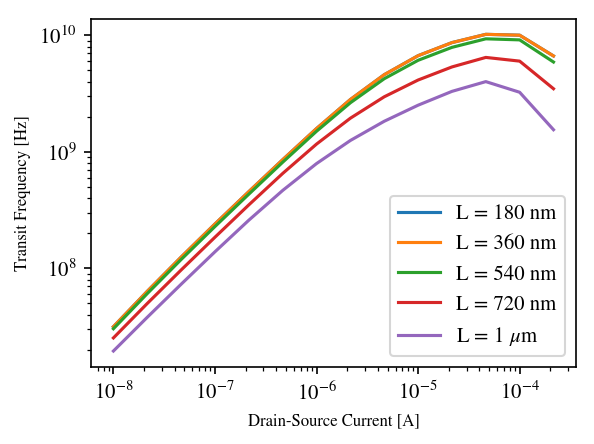
\includegraphics[width=\textwidth]{ft_nel_L}
		\resizebox {\textwidth} {!} {
			%% Creator: Matplotlib, PGF backend
%%
%% To include the figure in your LaTeX document, write
%%   \input{<filename>.pgf}
%%
%% Make sure the required packages are loaded in your preamble
%%   \usepackage{pgf}
%%
%% Figures using additional raster images can only be included by \input if
%% they are in the same directory as the main LaTeX file. For loading figures
%% from other directories you can use the `import` package
%%   \usepackage{import}
%% and then include the figures with
%%   \import{<path to file>}{<filename>.pgf}
%%
%% Matplotlib used the following preamble
%%   \usepackage{gensymb}
%%   \usepackage[utf8x]{inputenc}
%%   \usepackage[T1]{fontenc}
%%
\begingroup%
\makeatletter%
\begin{pgfpicture}%
\pgfpathrectangle{\pgfpointorigin}{\pgfqpoint{3.840000in}{2.840000in}}%
\pgfusepath{use as bounding box, clip}%
\begin{pgfscope}%
\pgfsetbuttcap%
\pgfsetmiterjoin%
\definecolor{currentfill}{rgb}{1.000000,1.000000,1.000000}%
\pgfsetfillcolor{currentfill}%
\pgfsetlinewidth{0.000000pt}%
\definecolor{currentstroke}{rgb}{1.000000,1.000000,1.000000}%
\pgfsetstrokecolor{currentstroke}%
\pgfsetdash{}{0pt}%
\pgfpathmoveto{\pgfqpoint{0.000000in}{0.000000in}}%
\pgfpathlineto{\pgfqpoint{3.840000in}{0.000000in}}%
\pgfpathlineto{\pgfqpoint{3.840000in}{2.840000in}}%
\pgfpathlineto{\pgfqpoint{0.000000in}{2.840000in}}%
\pgfpathclose%
\pgfusepath{fill}%
\end{pgfscope}%
\begin{pgfscope}%
\pgfsetbuttcap%
\pgfsetmiterjoin%
\definecolor{currentfill}{rgb}{1.000000,1.000000,1.000000}%
\pgfsetfillcolor{currentfill}%
\pgfsetlinewidth{0.000000pt}%
\definecolor{currentstroke}{rgb}{0.000000,0.000000,0.000000}%
\pgfsetstrokecolor{currentstroke}%
\pgfsetstrokeopacity{0.000000}%
\pgfsetdash{}{0pt}%
\pgfpathmoveto{\pgfqpoint{0.761068in}{0.596026in}}%
\pgfpathlineto{\pgfqpoint{3.716667in}{0.596026in}}%
\pgfpathlineto{\pgfqpoint{3.716667in}{2.716667in}}%
\pgfpathlineto{\pgfqpoint{0.761068in}{2.716667in}}%
\pgfpathclose%
\pgfusepath{fill}%
\end{pgfscope}%
\begin{pgfscope}%
\pgfsetbuttcap%
\pgfsetroundjoin%
\definecolor{currentfill}{rgb}{0.000000,0.000000,0.000000}%
\pgfsetfillcolor{currentfill}%
\pgfsetlinewidth{0.803000pt}%
\definecolor{currentstroke}{rgb}{0.000000,0.000000,0.000000}%
\pgfsetstrokecolor{currentstroke}%
\pgfsetdash{}{0pt}%
\pgfsys@defobject{currentmarker}{\pgfqpoint{0.000000in}{-0.048611in}}{\pgfqpoint{0.000000in}{0.000000in}}{%
\pgfpathmoveto{\pgfqpoint{0.000000in}{0.000000in}}%
\pgfpathlineto{\pgfqpoint{0.000000in}{-0.048611in}}%
\pgfusepath{stroke,fill}%
}%
\begin{pgfscope}%
\pgfsys@transformshift{0.895441in}{0.596026in}%
\pgfsys@useobject{currentmarker}{}%
\end{pgfscope}%
\end{pgfscope}%
\begin{pgfscope}%
\pgftext[x=0.895441in,y=0.498804in,,top]{\fontsize{14.000000}{16.800000}\selectfont \(\displaystyle 10^{-8}\)}%
\end{pgfscope}%
\begin{pgfscope}%
\pgfsetbuttcap%
\pgfsetroundjoin%
\definecolor{currentfill}{rgb}{0.000000,0.000000,0.000000}%
\pgfsetfillcolor{currentfill}%
\pgfsetlinewidth{0.803000pt}%
\definecolor{currentstroke}{rgb}{0.000000,0.000000,0.000000}%
\pgfsetstrokecolor{currentstroke}%
\pgfsetdash{}{0pt}%
\pgfsys@defobject{currentmarker}{\pgfqpoint{0.000000in}{-0.048611in}}{\pgfqpoint{0.000000in}{0.000000in}}{%
\pgfpathmoveto{\pgfqpoint{0.000000in}{0.000000in}}%
\pgfpathlineto{\pgfqpoint{0.000000in}{-0.048611in}}%
\pgfusepath{stroke,fill}%
}%
\begin{pgfscope}%
\pgfsys@transformshift{1.515503in}{0.596026in}%
\pgfsys@useobject{currentmarker}{}%
\end{pgfscope}%
\end{pgfscope}%
\begin{pgfscope}%
\pgftext[x=1.515503in,y=0.498804in,,top]{\fontsize{14.000000}{16.800000}\selectfont \(\displaystyle 10^{-7}\)}%
\end{pgfscope}%
\begin{pgfscope}%
\pgfsetbuttcap%
\pgfsetroundjoin%
\definecolor{currentfill}{rgb}{0.000000,0.000000,0.000000}%
\pgfsetfillcolor{currentfill}%
\pgfsetlinewidth{0.803000pt}%
\definecolor{currentstroke}{rgb}{0.000000,0.000000,0.000000}%
\pgfsetstrokecolor{currentstroke}%
\pgfsetdash{}{0pt}%
\pgfsys@defobject{currentmarker}{\pgfqpoint{0.000000in}{-0.048611in}}{\pgfqpoint{0.000000in}{0.000000in}}{%
\pgfpathmoveto{\pgfqpoint{0.000000in}{0.000000in}}%
\pgfpathlineto{\pgfqpoint{0.000000in}{-0.048611in}}%
\pgfusepath{stroke,fill}%
}%
\begin{pgfscope}%
\pgfsys@transformshift{2.135564in}{0.596026in}%
\pgfsys@useobject{currentmarker}{}%
\end{pgfscope}%
\end{pgfscope}%
\begin{pgfscope}%
\pgftext[x=2.135564in,y=0.498804in,,top]{\fontsize{14.000000}{16.800000}\selectfont \(\displaystyle 10^{-6}\)}%
\end{pgfscope}%
\begin{pgfscope}%
\pgfsetbuttcap%
\pgfsetroundjoin%
\definecolor{currentfill}{rgb}{0.000000,0.000000,0.000000}%
\pgfsetfillcolor{currentfill}%
\pgfsetlinewidth{0.803000pt}%
\definecolor{currentstroke}{rgb}{0.000000,0.000000,0.000000}%
\pgfsetstrokecolor{currentstroke}%
\pgfsetdash{}{0pt}%
\pgfsys@defobject{currentmarker}{\pgfqpoint{0.000000in}{-0.048611in}}{\pgfqpoint{0.000000in}{0.000000in}}{%
\pgfpathmoveto{\pgfqpoint{0.000000in}{0.000000in}}%
\pgfpathlineto{\pgfqpoint{0.000000in}{-0.048611in}}%
\pgfusepath{stroke,fill}%
}%
\begin{pgfscope}%
\pgfsys@transformshift{2.755626in}{0.596026in}%
\pgfsys@useobject{currentmarker}{}%
\end{pgfscope}%
\end{pgfscope}%
\begin{pgfscope}%
\pgftext[x=2.755626in,y=0.498804in,,top]{\fontsize{14.000000}{16.800000}\selectfont \(\displaystyle 10^{-5}\)}%
\end{pgfscope}%
\begin{pgfscope}%
\pgfsetbuttcap%
\pgfsetroundjoin%
\definecolor{currentfill}{rgb}{0.000000,0.000000,0.000000}%
\pgfsetfillcolor{currentfill}%
\pgfsetlinewidth{0.803000pt}%
\definecolor{currentstroke}{rgb}{0.000000,0.000000,0.000000}%
\pgfsetstrokecolor{currentstroke}%
\pgfsetdash{}{0pt}%
\pgfsys@defobject{currentmarker}{\pgfqpoint{0.000000in}{-0.048611in}}{\pgfqpoint{0.000000in}{0.000000in}}{%
\pgfpathmoveto{\pgfqpoint{0.000000in}{0.000000in}}%
\pgfpathlineto{\pgfqpoint{0.000000in}{-0.048611in}}%
\pgfusepath{stroke,fill}%
}%
\begin{pgfscope}%
\pgfsys@transformshift{3.375688in}{0.596026in}%
\pgfsys@useobject{currentmarker}{}%
\end{pgfscope}%
\end{pgfscope}%
\begin{pgfscope}%
\pgftext[x=3.375688in,y=0.498804in,,top]{\fontsize{14.000000}{16.800000}\selectfont \(\displaystyle 10^{-4}\)}%
\end{pgfscope}%
\begin{pgfscope}%
\pgfsetbuttcap%
\pgfsetroundjoin%
\definecolor{currentfill}{rgb}{0.000000,0.000000,0.000000}%
\pgfsetfillcolor{currentfill}%
\pgfsetlinewidth{0.602250pt}%
\definecolor{currentstroke}{rgb}{0.000000,0.000000,0.000000}%
\pgfsetstrokecolor{currentstroke}%
\pgfsetdash{}{0pt}%
\pgfsys@defobject{currentmarker}{\pgfqpoint{0.000000in}{-0.027778in}}{\pgfqpoint{0.000000in}{0.000000in}}{%
\pgfpathmoveto{\pgfqpoint{0.000000in}{0.000000in}}%
\pgfpathlineto{\pgfqpoint{0.000000in}{-0.027778in}}%
\pgfusepath{stroke,fill}%
}%
\begin{pgfscope}%
\pgfsys@transformshift{0.757881in}{0.596026in}%
\pgfsys@useobject{currentmarker}{}%
\end{pgfscope}%
\end{pgfscope}%
\begin{pgfscope}%
\pgfsetbuttcap%
\pgfsetroundjoin%
\definecolor{currentfill}{rgb}{0.000000,0.000000,0.000000}%
\pgfsetfillcolor{currentfill}%
\pgfsetlinewidth{0.602250pt}%
\definecolor{currentstroke}{rgb}{0.000000,0.000000,0.000000}%
\pgfsetstrokecolor{currentstroke}%
\pgfsetdash{}{0pt}%
\pgfsys@defobject{currentmarker}{\pgfqpoint{0.000000in}{-0.027778in}}{\pgfqpoint{0.000000in}{0.000000in}}{%
\pgfpathmoveto{\pgfqpoint{0.000000in}{0.000000in}}%
\pgfpathlineto{\pgfqpoint{0.000000in}{-0.027778in}}%
\pgfusepath{stroke,fill}%
}%
\begin{pgfscope}%
\pgfsys@transformshift{0.799392in}{0.596026in}%
\pgfsys@useobject{currentmarker}{}%
\end{pgfscope}%
\end{pgfscope}%
\begin{pgfscope}%
\pgfsetbuttcap%
\pgfsetroundjoin%
\definecolor{currentfill}{rgb}{0.000000,0.000000,0.000000}%
\pgfsetfillcolor{currentfill}%
\pgfsetlinewidth{0.602250pt}%
\definecolor{currentstroke}{rgb}{0.000000,0.000000,0.000000}%
\pgfsetstrokecolor{currentstroke}%
\pgfsetdash{}{0pt}%
\pgfsys@defobject{currentmarker}{\pgfqpoint{0.000000in}{-0.027778in}}{\pgfqpoint{0.000000in}{0.000000in}}{%
\pgfpathmoveto{\pgfqpoint{0.000000in}{0.000000in}}%
\pgfpathlineto{\pgfqpoint{0.000000in}{-0.027778in}}%
\pgfusepath{stroke,fill}%
}%
\begin{pgfscope}%
\pgfsys@transformshift{0.835350in}{0.596026in}%
\pgfsys@useobject{currentmarker}{}%
\end{pgfscope}%
\end{pgfscope}%
\begin{pgfscope}%
\pgfsetbuttcap%
\pgfsetroundjoin%
\definecolor{currentfill}{rgb}{0.000000,0.000000,0.000000}%
\pgfsetfillcolor{currentfill}%
\pgfsetlinewidth{0.602250pt}%
\definecolor{currentstroke}{rgb}{0.000000,0.000000,0.000000}%
\pgfsetstrokecolor{currentstroke}%
\pgfsetdash{}{0pt}%
\pgfsys@defobject{currentmarker}{\pgfqpoint{0.000000in}{-0.027778in}}{\pgfqpoint{0.000000in}{0.000000in}}{%
\pgfpathmoveto{\pgfqpoint{0.000000in}{0.000000in}}%
\pgfpathlineto{\pgfqpoint{0.000000in}{-0.027778in}}%
\pgfusepath{stroke,fill}%
}%
\begin{pgfscope}%
\pgfsys@transformshift{0.867068in}{0.596026in}%
\pgfsys@useobject{currentmarker}{}%
\end{pgfscope}%
\end{pgfscope}%
\begin{pgfscope}%
\pgfsetbuttcap%
\pgfsetroundjoin%
\definecolor{currentfill}{rgb}{0.000000,0.000000,0.000000}%
\pgfsetfillcolor{currentfill}%
\pgfsetlinewidth{0.602250pt}%
\definecolor{currentstroke}{rgb}{0.000000,0.000000,0.000000}%
\pgfsetstrokecolor{currentstroke}%
\pgfsetdash{}{0pt}%
\pgfsys@defobject{currentmarker}{\pgfqpoint{0.000000in}{-0.027778in}}{\pgfqpoint{0.000000in}{0.000000in}}{%
\pgfpathmoveto{\pgfqpoint{0.000000in}{0.000000in}}%
\pgfpathlineto{\pgfqpoint{0.000000in}{-0.027778in}}%
\pgfusepath{stroke,fill}%
}%
\begin{pgfscope}%
\pgfsys@transformshift{1.082098in}{0.596026in}%
\pgfsys@useobject{currentmarker}{}%
\end{pgfscope}%
\end{pgfscope}%
\begin{pgfscope}%
\pgfsetbuttcap%
\pgfsetroundjoin%
\definecolor{currentfill}{rgb}{0.000000,0.000000,0.000000}%
\pgfsetfillcolor{currentfill}%
\pgfsetlinewidth{0.602250pt}%
\definecolor{currentstroke}{rgb}{0.000000,0.000000,0.000000}%
\pgfsetstrokecolor{currentstroke}%
\pgfsetdash{}{0pt}%
\pgfsys@defobject{currentmarker}{\pgfqpoint{0.000000in}{-0.027778in}}{\pgfqpoint{0.000000in}{0.000000in}}{%
\pgfpathmoveto{\pgfqpoint{0.000000in}{0.000000in}}%
\pgfpathlineto{\pgfqpoint{0.000000in}{-0.027778in}}%
\pgfusepath{stroke,fill}%
}%
\begin{pgfscope}%
\pgfsys@transformshift{1.191285in}{0.596026in}%
\pgfsys@useobject{currentmarker}{}%
\end{pgfscope}%
\end{pgfscope}%
\begin{pgfscope}%
\pgfsetbuttcap%
\pgfsetroundjoin%
\definecolor{currentfill}{rgb}{0.000000,0.000000,0.000000}%
\pgfsetfillcolor{currentfill}%
\pgfsetlinewidth{0.602250pt}%
\definecolor{currentstroke}{rgb}{0.000000,0.000000,0.000000}%
\pgfsetstrokecolor{currentstroke}%
\pgfsetdash{}{0pt}%
\pgfsys@defobject{currentmarker}{\pgfqpoint{0.000000in}{-0.027778in}}{\pgfqpoint{0.000000in}{0.000000in}}{%
\pgfpathmoveto{\pgfqpoint{0.000000in}{0.000000in}}%
\pgfpathlineto{\pgfqpoint{0.000000in}{-0.027778in}}%
\pgfusepath{stroke,fill}%
}%
\begin{pgfscope}%
\pgfsys@transformshift{1.268755in}{0.596026in}%
\pgfsys@useobject{currentmarker}{}%
\end{pgfscope}%
\end{pgfscope}%
\begin{pgfscope}%
\pgfsetbuttcap%
\pgfsetroundjoin%
\definecolor{currentfill}{rgb}{0.000000,0.000000,0.000000}%
\pgfsetfillcolor{currentfill}%
\pgfsetlinewidth{0.602250pt}%
\definecolor{currentstroke}{rgb}{0.000000,0.000000,0.000000}%
\pgfsetstrokecolor{currentstroke}%
\pgfsetdash{}{0pt}%
\pgfsys@defobject{currentmarker}{\pgfqpoint{0.000000in}{-0.027778in}}{\pgfqpoint{0.000000in}{0.000000in}}{%
\pgfpathmoveto{\pgfqpoint{0.000000in}{0.000000in}}%
\pgfpathlineto{\pgfqpoint{0.000000in}{-0.027778in}}%
\pgfusepath{stroke,fill}%
}%
\begin{pgfscope}%
\pgfsys@transformshift{1.328845in}{0.596026in}%
\pgfsys@useobject{currentmarker}{}%
\end{pgfscope}%
\end{pgfscope}%
\begin{pgfscope}%
\pgfsetbuttcap%
\pgfsetroundjoin%
\definecolor{currentfill}{rgb}{0.000000,0.000000,0.000000}%
\pgfsetfillcolor{currentfill}%
\pgfsetlinewidth{0.602250pt}%
\definecolor{currentstroke}{rgb}{0.000000,0.000000,0.000000}%
\pgfsetstrokecolor{currentstroke}%
\pgfsetdash{}{0pt}%
\pgfsys@defobject{currentmarker}{\pgfqpoint{0.000000in}{-0.027778in}}{\pgfqpoint{0.000000in}{0.000000in}}{%
\pgfpathmoveto{\pgfqpoint{0.000000in}{0.000000in}}%
\pgfpathlineto{\pgfqpoint{0.000000in}{-0.027778in}}%
\pgfusepath{stroke,fill}%
}%
\begin{pgfscope}%
\pgfsys@transformshift{1.377943in}{0.596026in}%
\pgfsys@useobject{currentmarker}{}%
\end{pgfscope}%
\end{pgfscope}%
\begin{pgfscope}%
\pgfsetbuttcap%
\pgfsetroundjoin%
\definecolor{currentfill}{rgb}{0.000000,0.000000,0.000000}%
\pgfsetfillcolor{currentfill}%
\pgfsetlinewidth{0.602250pt}%
\definecolor{currentstroke}{rgb}{0.000000,0.000000,0.000000}%
\pgfsetstrokecolor{currentstroke}%
\pgfsetdash{}{0pt}%
\pgfsys@defobject{currentmarker}{\pgfqpoint{0.000000in}{-0.027778in}}{\pgfqpoint{0.000000in}{0.000000in}}{%
\pgfpathmoveto{\pgfqpoint{0.000000in}{0.000000in}}%
\pgfpathlineto{\pgfqpoint{0.000000in}{-0.027778in}}%
\pgfusepath{stroke,fill}%
}%
\begin{pgfscope}%
\pgfsys@transformshift{1.419454in}{0.596026in}%
\pgfsys@useobject{currentmarker}{}%
\end{pgfscope}%
\end{pgfscope}%
\begin{pgfscope}%
\pgfsetbuttcap%
\pgfsetroundjoin%
\definecolor{currentfill}{rgb}{0.000000,0.000000,0.000000}%
\pgfsetfillcolor{currentfill}%
\pgfsetlinewidth{0.602250pt}%
\definecolor{currentstroke}{rgb}{0.000000,0.000000,0.000000}%
\pgfsetstrokecolor{currentstroke}%
\pgfsetdash{}{0pt}%
\pgfsys@defobject{currentmarker}{\pgfqpoint{0.000000in}{-0.027778in}}{\pgfqpoint{0.000000in}{0.000000in}}{%
\pgfpathmoveto{\pgfqpoint{0.000000in}{0.000000in}}%
\pgfpathlineto{\pgfqpoint{0.000000in}{-0.027778in}}%
\pgfusepath{stroke,fill}%
}%
\begin{pgfscope}%
\pgfsys@transformshift{1.455412in}{0.596026in}%
\pgfsys@useobject{currentmarker}{}%
\end{pgfscope}%
\end{pgfscope}%
\begin{pgfscope}%
\pgfsetbuttcap%
\pgfsetroundjoin%
\definecolor{currentfill}{rgb}{0.000000,0.000000,0.000000}%
\pgfsetfillcolor{currentfill}%
\pgfsetlinewidth{0.602250pt}%
\definecolor{currentstroke}{rgb}{0.000000,0.000000,0.000000}%
\pgfsetstrokecolor{currentstroke}%
\pgfsetdash{}{0pt}%
\pgfsys@defobject{currentmarker}{\pgfqpoint{0.000000in}{-0.027778in}}{\pgfqpoint{0.000000in}{0.000000in}}{%
\pgfpathmoveto{\pgfqpoint{0.000000in}{0.000000in}}%
\pgfpathlineto{\pgfqpoint{0.000000in}{-0.027778in}}%
\pgfusepath{stroke,fill}%
}%
\begin{pgfscope}%
\pgfsys@transformshift{1.487130in}{0.596026in}%
\pgfsys@useobject{currentmarker}{}%
\end{pgfscope}%
\end{pgfscope}%
\begin{pgfscope}%
\pgfsetbuttcap%
\pgfsetroundjoin%
\definecolor{currentfill}{rgb}{0.000000,0.000000,0.000000}%
\pgfsetfillcolor{currentfill}%
\pgfsetlinewidth{0.602250pt}%
\definecolor{currentstroke}{rgb}{0.000000,0.000000,0.000000}%
\pgfsetstrokecolor{currentstroke}%
\pgfsetdash{}{0pt}%
\pgfsys@defobject{currentmarker}{\pgfqpoint{0.000000in}{-0.027778in}}{\pgfqpoint{0.000000in}{0.000000in}}{%
\pgfpathmoveto{\pgfqpoint{0.000000in}{0.000000in}}%
\pgfpathlineto{\pgfqpoint{0.000000in}{-0.027778in}}%
\pgfusepath{stroke,fill}%
}%
\begin{pgfscope}%
\pgfsys@transformshift{1.702160in}{0.596026in}%
\pgfsys@useobject{currentmarker}{}%
\end{pgfscope}%
\end{pgfscope}%
\begin{pgfscope}%
\pgfsetbuttcap%
\pgfsetroundjoin%
\definecolor{currentfill}{rgb}{0.000000,0.000000,0.000000}%
\pgfsetfillcolor{currentfill}%
\pgfsetlinewidth{0.602250pt}%
\definecolor{currentstroke}{rgb}{0.000000,0.000000,0.000000}%
\pgfsetstrokecolor{currentstroke}%
\pgfsetdash{}{0pt}%
\pgfsys@defobject{currentmarker}{\pgfqpoint{0.000000in}{-0.027778in}}{\pgfqpoint{0.000000in}{0.000000in}}{%
\pgfpathmoveto{\pgfqpoint{0.000000in}{0.000000in}}%
\pgfpathlineto{\pgfqpoint{0.000000in}{-0.027778in}}%
\pgfusepath{stroke,fill}%
}%
\begin{pgfscope}%
\pgfsys@transformshift{1.811347in}{0.596026in}%
\pgfsys@useobject{currentmarker}{}%
\end{pgfscope}%
\end{pgfscope}%
\begin{pgfscope}%
\pgfsetbuttcap%
\pgfsetroundjoin%
\definecolor{currentfill}{rgb}{0.000000,0.000000,0.000000}%
\pgfsetfillcolor{currentfill}%
\pgfsetlinewidth{0.602250pt}%
\definecolor{currentstroke}{rgb}{0.000000,0.000000,0.000000}%
\pgfsetstrokecolor{currentstroke}%
\pgfsetdash{}{0pt}%
\pgfsys@defobject{currentmarker}{\pgfqpoint{0.000000in}{-0.027778in}}{\pgfqpoint{0.000000in}{0.000000in}}{%
\pgfpathmoveto{\pgfqpoint{0.000000in}{0.000000in}}%
\pgfpathlineto{\pgfqpoint{0.000000in}{-0.027778in}}%
\pgfusepath{stroke,fill}%
}%
\begin{pgfscope}%
\pgfsys@transformshift{1.888817in}{0.596026in}%
\pgfsys@useobject{currentmarker}{}%
\end{pgfscope}%
\end{pgfscope}%
\begin{pgfscope}%
\pgfsetbuttcap%
\pgfsetroundjoin%
\definecolor{currentfill}{rgb}{0.000000,0.000000,0.000000}%
\pgfsetfillcolor{currentfill}%
\pgfsetlinewidth{0.602250pt}%
\definecolor{currentstroke}{rgb}{0.000000,0.000000,0.000000}%
\pgfsetstrokecolor{currentstroke}%
\pgfsetdash{}{0pt}%
\pgfsys@defobject{currentmarker}{\pgfqpoint{0.000000in}{-0.027778in}}{\pgfqpoint{0.000000in}{0.000000in}}{%
\pgfpathmoveto{\pgfqpoint{0.000000in}{0.000000in}}%
\pgfpathlineto{\pgfqpoint{0.000000in}{-0.027778in}}%
\pgfusepath{stroke,fill}%
}%
\begin{pgfscope}%
\pgfsys@transformshift{1.948907in}{0.596026in}%
\pgfsys@useobject{currentmarker}{}%
\end{pgfscope}%
\end{pgfscope}%
\begin{pgfscope}%
\pgfsetbuttcap%
\pgfsetroundjoin%
\definecolor{currentfill}{rgb}{0.000000,0.000000,0.000000}%
\pgfsetfillcolor{currentfill}%
\pgfsetlinewidth{0.602250pt}%
\definecolor{currentstroke}{rgb}{0.000000,0.000000,0.000000}%
\pgfsetstrokecolor{currentstroke}%
\pgfsetdash{}{0pt}%
\pgfsys@defobject{currentmarker}{\pgfqpoint{0.000000in}{-0.027778in}}{\pgfqpoint{0.000000in}{0.000000in}}{%
\pgfpathmoveto{\pgfqpoint{0.000000in}{0.000000in}}%
\pgfpathlineto{\pgfqpoint{0.000000in}{-0.027778in}}%
\pgfusepath{stroke,fill}%
}%
\begin{pgfscope}%
\pgfsys@transformshift{1.998005in}{0.596026in}%
\pgfsys@useobject{currentmarker}{}%
\end{pgfscope}%
\end{pgfscope}%
\begin{pgfscope}%
\pgfsetbuttcap%
\pgfsetroundjoin%
\definecolor{currentfill}{rgb}{0.000000,0.000000,0.000000}%
\pgfsetfillcolor{currentfill}%
\pgfsetlinewidth{0.602250pt}%
\definecolor{currentstroke}{rgb}{0.000000,0.000000,0.000000}%
\pgfsetstrokecolor{currentstroke}%
\pgfsetdash{}{0pt}%
\pgfsys@defobject{currentmarker}{\pgfqpoint{0.000000in}{-0.027778in}}{\pgfqpoint{0.000000in}{0.000000in}}{%
\pgfpathmoveto{\pgfqpoint{0.000000in}{0.000000in}}%
\pgfpathlineto{\pgfqpoint{0.000000in}{-0.027778in}}%
\pgfusepath{stroke,fill}%
}%
\begin{pgfscope}%
\pgfsys@transformshift{2.039516in}{0.596026in}%
\pgfsys@useobject{currentmarker}{}%
\end{pgfscope}%
\end{pgfscope}%
\begin{pgfscope}%
\pgfsetbuttcap%
\pgfsetroundjoin%
\definecolor{currentfill}{rgb}{0.000000,0.000000,0.000000}%
\pgfsetfillcolor{currentfill}%
\pgfsetlinewidth{0.602250pt}%
\definecolor{currentstroke}{rgb}{0.000000,0.000000,0.000000}%
\pgfsetstrokecolor{currentstroke}%
\pgfsetdash{}{0pt}%
\pgfsys@defobject{currentmarker}{\pgfqpoint{0.000000in}{-0.027778in}}{\pgfqpoint{0.000000in}{0.000000in}}{%
\pgfpathmoveto{\pgfqpoint{0.000000in}{0.000000in}}%
\pgfpathlineto{\pgfqpoint{0.000000in}{-0.027778in}}%
\pgfusepath{stroke,fill}%
}%
\begin{pgfscope}%
\pgfsys@transformshift{2.075474in}{0.596026in}%
\pgfsys@useobject{currentmarker}{}%
\end{pgfscope}%
\end{pgfscope}%
\begin{pgfscope}%
\pgfsetbuttcap%
\pgfsetroundjoin%
\definecolor{currentfill}{rgb}{0.000000,0.000000,0.000000}%
\pgfsetfillcolor{currentfill}%
\pgfsetlinewidth{0.602250pt}%
\definecolor{currentstroke}{rgb}{0.000000,0.000000,0.000000}%
\pgfsetstrokecolor{currentstroke}%
\pgfsetdash{}{0pt}%
\pgfsys@defobject{currentmarker}{\pgfqpoint{0.000000in}{-0.027778in}}{\pgfqpoint{0.000000in}{0.000000in}}{%
\pgfpathmoveto{\pgfqpoint{0.000000in}{0.000000in}}%
\pgfpathlineto{\pgfqpoint{0.000000in}{-0.027778in}}%
\pgfusepath{stroke,fill}%
}%
\begin{pgfscope}%
\pgfsys@transformshift{2.107192in}{0.596026in}%
\pgfsys@useobject{currentmarker}{}%
\end{pgfscope}%
\end{pgfscope}%
\begin{pgfscope}%
\pgfsetbuttcap%
\pgfsetroundjoin%
\definecolor{currentfill}{rgb}{0.000000,0.000000,0.000000}%
\pgfsetfillcolor{currentfill}%
\pgfsetlinewidth{0.602250pt}%
\definecolor{currentstroke}{rgb}{0.000000,0.000000,0.000000}%
\pgfsetstrokecolor{currentstroke}%
\pgfsetdash{}{0pt}%
\pgfsys@defobject{currentmarker}{\pgfqpoint{0.000000in}{-0.027778in}}{\pgfqpoint{0.000000in}{0.000000in}}{%
\pgfpathmoveto{\pgfqpoint{0.000000in}{0.000000in}}%
\pgfpathlineto{\pgfqpoint{0.000000in}{-0.027778in}}%
\pgfusepath{stroke,fill}%
}%
\begin{pgfscope}%
\pgfsys@transformshift{2.322222in}{0.596026in}%
\pgfsys@useobject{currentmarker}{}%
\end{pgfscope}%
\end{pgfscope}%
\begin{pgfscope}%
\pgfsetbuttcap%
\pgfsetroundjoin%
\definecolor{currentfill}{rgb}{0.000000,0.000000,0.000000}%
\pgfsetfillcolor{currentfill}%
\pgfsetlinewidth{0.602250pt}%
\definecolor{currentstroke}{rgb}{0.000000,0.000000,0.000000}%
\pgfsetstrokecolor{currentstroke}%
\pgfsetdash{}{0pt}%
\pgfsys@defobject{currentmarker}{\pgfqpoint{0.000000in}{-0.027778in}}{\pgfqpoint{0.000000in}{0.000000in}}{%
\pgfpathmoveto{\pgfqpoint{0.000000in}{0.000000in}}%
\pgfpathlineto{\pgfqpoint{0.000000in}{-0.027778in}}%
\pgfusepath{stroke,fill}%
}%
\begin{pgfscope}%
\pgfsys@transformshift{2.431409in}{0.596026in}%
\pgfsys@useobject{currentmarker}{}%
\end{pgfscope}%
\end{pgfscope}%
\begin{pgfscope}%
\pgfsetbuttcap%
\pgfsetroundjoin%
\definecolor{currentfill}{rgb}{0.000000,0.000000,0.000000}%
\pgfsetfillcolor{currentfill}%
\pgfsetlinewidth{0.602250pt}%
\definecolor{currentstroke}{rgb}{0.000000,0.000000,0.000000}%
\pgfsetstrokecolor{currentstroke}%
\pgfsetdash{}{0pt}%
\pgfsys@defobject{currentmarker}{\pgfqpoint{0.000000in}{-0.027778in}}{\pgfqpoint{0.000000in}{0.000000in}}{%
\pgfpathmoveto{\pgfqpoint{0.000000in}{0.000000in}}%
\pgfpathlineto{\pgfqpoint{0.000000in}{-0.027778in}}%
\pgfusepath{stroke,fill}%
}%
\begin{pgfscope}%
\pgfsys@transformshift{2.508879in}{0.596026in}%
\pgfsys@useobject{currentmarker}{}%
\end{pgfscope}%
\end{pgfscope}%
\begin{pgfscope}%
\pgfsetbuttcap%
\pgfsetroundjoin%
\definecolor{currentfill}{rgb}{0.000000,0.000000,0.000000}%
\pgfsetfillcolor{currentfill}%
\pgfsetlinewidth{0.602250pt}%
\definecolor{currentstroke}{rgb}{0.000000,0.000000,0.000000}%
\pgfsetstrokecolor{currentstroke}%
\pgfsetdash{}{0pt}%
\pgfsys@defobject{currentmarker}{\pgfqpoint{0.000000in}{-0.027778in}}{\pgfqpoint{0.000000in}{0.000000in}}{%
\pgfpathmoveto{\pgfqpoint{0.000000in}{0.000000in}}%
\pgfpathlineto{\pgfqpoint{0.000000in}{-0.027778in}}%
\pgfusepath{stroke,fill}%
}%
\begin{pgfscope}%
\pgfsys@transformshift{2.568969in}{0.596026in}%
\pgfsys@useobject{currentmarker}{}%
\end{pgfscope}%
\end{pgfscope}%
\begin{pgfscope}%
\pgfsetbuttcap%
\pgfsetroundjoin%
\definecolor{currentfill}{rgb}{0.000000,0.000000,0.000000}%
\pgfsetfillcolor{currentfill}%
\pgfsetlinewidth{0.602250pt}%
\definecolor{currentstroke}{rgb}{0.000000,0.000000,0.000000}%
\pgfsetstrokecolor{currentstroke}%
\pgfsetdash{}{0pt}%
\pgfsys@defobject{currentmarker}{\pgfqpoint{0.000000in}{-0.027778in}}{\pgfqpoint{0.000000in}{0.000000in}}{%
\pgfpathmoveto{\pgfqpoint{0.000000in}{0.000000in}}%
\pgfpathlineto{\pgfqpoint{0.000000in}{-0.027778in}}%
\pgfusepath{stroke,fill}%
}%
\begin{pgfscope}%
\pgfsys@transformshift{2.618066in}{0.596026in}%
\pgfsys@useobject{currentmarker}{}%
\end{pgfscope}%
\end{pgfscope}%
\begin{pgfscope}%
\pgfsetbuttcap%
\pgfsetroundjoin%
\definecolor{currentfill}{rgb}{0.000000,0.000000,0.000000}%
\pgfsetfillcolor{currentfill}%
\pgfsetlinewidth{0.602250pt}%
\definecolor{currentstroke}{rgb}{0.000000,0.000000,0.000000}%
\pgfsetstrokecolor{currentstroke}%
\pgfsetdash{}{0pt}%
\pgfsys@defobject{currentmarker}{\pgfqpoint{0.000000in}{-0.027778in}}{\pgfqpoint{0.000000in}{0.000000in}}{%
\pgfpathmoveto{\pgfqpoint{0.000000in}{0.000000in}}%
\pgfpathlineto{\pgfqpoint{0.000000in}{-0.027778in}}%
\pgfusepath{stroke,fill}%
}%
\begin{pgfscope}%
\pgfsys@transformshift{2.659578in}{0.596026in}%
\pgfsys@useobject{currentmarker}{}%
\end{pgfscope}%
\end{pgfscope}%
\begin{pgfscope}%
\pgfsetbuttcap%
\pgfsetroundjoin%
\definecolor{currentfill}{rgb}{0.000000,0.000000,0.000000}%
\pgfsetfillcolor{currentfill}%
\pgfsetlinewidth{0.602250pt}%
\definecolor{currentstroke}{rgb}{0.000000,0.000000,0.000000}%
\pgfsetstrokecolor{currentstroke}%
\pgfsetdash{}{0pt}%
\pgfsys@defobject{currentmarker}{\pgfqpoint{0.000000in}{-0.027778in}}{\pgfqpoint{0.000000in}{0.000000in}}{%
\pgfpathmoveto{\pgfqpoint{0.000000in}{0.000000in}}%
\pgfpathlineto{\pgfqpoint{0.000000in}{-0.027778in}}%
\pgfusepath{stroke,fill}%
}%
\begin{pgfscope}%
\pgfsys@transformshift{2.695536in}{0.596026in}%
\pgfsys@useobject{currentmarker}{}%
\end{pgfscope}%
\end{pgfscope}%
\begin{pgfscope}%
\pgfsetbuttcap%
\pgfsetroundjoin%
\definecolor{currentfill}{rgb}{0.000000,0.000000,0.000000}%
\pgfsetfillcolor{currentfill}%
\pgfsetlinewidth{0.602250pt}%
\definecolor{currentstroke}{rgb}{0.000000,0.000000,0.000000}%
\pgfsetstrokecolor{currentstroke}%
\pgfsetdash{}{0pt}%
\pgfsys@defobject{currentmarker}{\pgfqpoint{0.000000in}{-0.027778in}}{\pgfqpoint{0.000000in}{0.000000in}}{%
\pgfpathmoveto{\pgfqpoint{0.000000in}{0.000000in}}%
\pgfpathlineto{\pgfqpoint{0.000000in}{-0.027778in}}%
\pgfusepath{stroke,fill}%
}%
\begin{pgfscope}%
\pgfsys@transformshift{2.727254in}{0.596026in}%
\pgfsys@useobject{currentmarker}{}%
\end{pgfscope}%
\end{pgfscope}%
\begin{pgfscope}%
\pgfsetbuttcap%
\pgfsetroundjoin%
\definecolor{currentfill}{rgb}{0.000000,0.000000,0.000000}%
\pgfsetfillcolor{currentfill}%
\pgfsetlinewidth{0.602250pt}%
\definecolor{currentstroke}{rgb}{0.000000,0.000000,0.000000}%
\pgfsetstrokecolor{currentstroke}%
\pgfsetdash{}{0pt}%
\pgfsys@defobject{currentmarker}{\pgfqpoint{0.000000in}{-0.027778in}}{\pgfqpoint{0.000000in}{0.000000in}}{%
\pgfpathmoveto{\pgfqpoint{0.000000in}{0.000000in}}%
\pgfpathlineto{\pgfqpoint{0.000000in}{-0.027778in}}%
\pgfusepath{stroke,fill}%
}%
\begin{pgfscope}%
\pgfsys@transformshift{2.942284in}{0.596026in}%
\pgfsys@useobject{currentmarker}{}%
\end{pgfscope}%
\end{pgfscope}%
\begin{pgfscope}%
\pgfsetbuttcap%
\pgfsetroundjoin%
\definecolor{currentfill}{rgb}{0.000000,0.000000,0.000000}%
\pgfsetfillcolor{currentfill}%
\pgfsetlinewidth{0.602250pt}%
\definecolor{currentstroke}{rgb}{0.000000,0.000000,0.000000}%
\pgfsetstrokecolor{currentstroke}%
\pgfsetdash{}{0pt}%
\pgfsys@defobject{currentmarker}{\pgfqpoint{0.000000in}{-0.027778in}}{\pgfqpoint{0.000000in}{0.000000in}}{%
\pgfpathmoveto{\pgfqpoint{0.000000in}{0.000000in}}%
\pgfpathlineto{\pgfqpoint{0.000000in}{-0.027778in}}%
\pgfusepath{stroke,fill}%
}%
\begin{pgfscope}%
\pgfsys@transformshift{3.051471in}{0.596026in}%
\pgfsys@useobject{currentmarker}{}%
\end{pgfscope}%
\end{pgfscope}%
\begin{pgfscope}%
\pgfsetbuttcap%
\pgfsetroundjoin%
\definecolor{currentfill}{rgb}{0.000000,0.000000,0.000000}%
\pgfsetfillcolor{currentfill}%
\pgfsetlinewidth{0.602250pt}%
\definecolor{currentstroke}{rgb}{0.000000,0.000000,0.000000}%
\pgfsetstrokecolor{currentstroke}%
\pgfsetdash{}{0pt}%
\pgfsys@defobject{currentmarker}{\pgfqpoint{0.000000in}{-0.027778in}}{\pgfqpoint{0.000000in}{0.000000in}}{%
\pgfpathmoveto{\pgfqpoint{0.000000in}{0.000000in}}%
\pgfpathlineto{\pgfqpoint{0.000000in}{-0.027778in}}%
\pgfusepath{stroke,fill}%
}%
\begin{pgfscope}%
\pgfsys@transformshift{3.128941in}{0.596026in}%
\pgfsys@useobject{currentmarker}{}%
\end{pgfscope}%
\end{pgfscope}%
\begin{pgfscope}%
\pgfsetbuttcap%
\pgfsetroundjoin%
\definecolor{currentfill}{rgb}{0.000000,0.000000,0.000000}%
\pgfsetfillcolor{currentfill}%
\pgfsetlinewidth{0.602250pt}%
\definecolor{currentstroke}{rgb}{0.000000,0.000000,0.000000}%
\pgfsetstrokecolor{currentstroke}%
\pgfsetdash{}{0pt}%
\pgfsys@defobject{currentmarker}{\pgfqpoint{0.000000in}{-0.027778in}}{\pgfqpoint{0.000000in}{0.000000in}}{%
\pgfpathmoveto{\pgfqpoint{0.000000in}{0.000000in}}%
\pgfpathlineto{\pgfqpoint{0.000000in}{-0.027778in}}%
\pgfusepath{stroke,fill}%
}%
\begin{pgfscope}%
\pgfsys@transformshift{3.189031in}{0.596026in}%
\pgfsys@useobject{currentmarker}{}%
\end{pgfscope}%
\end{pgfscope}%
\begin{pgfscope}%
\pgfsetbuttcap%
\pgfsetroundjoin%
\definecolor{currentfill}{rgb}{0.000000,0.000000,0.000000}%
\pgfsetfillcolor{currentfill}%
\pgfsetlinewidth{0.602250pt}%
\definecolor{currentstroke}{rgb}{0.000000,0.000000,0.000000}%
\pgfsetstrokecolor{currentstroke}%
\pgfsetdash{}{0pt}%
\pgfsys@defobject{currentmarker}{\pgfqpoint{0.000000in}{-0.027778in}}{\pgfqpoint{0.000000in}{0.000000in}}{%
\pgfpathmoveto{\pgfqpoint{0.000000in}{0.000000in}}%
\pgfpathlineto{\pgfqpoint{0.000000in}{-0.027778in}}%
\pgfusepath{stroke,fill}%
}%
\begin{pgfscope}%
\pgfsys@transformshift{3.238128in}{0.596026in}%
\pgfsys@useobject{currentmarker}{}%
\end{pgfscope}%
\end{pgfscope}%
\begin{pgfscope}%
\pgfsetbuttcap%
\pgfsetroundjoin%
\definecolor{currentfill}{rgb}{0.000000,0.000000,0.000000}%
\pgfsetfillcolor{currentfill}%
\pgfsetlinewidth{0.602250pt}%
\definecolor{currentstroke}{rgb}{0.000000,0.000000,0.000000}%
\pgfsetstrokecolor{currentstroke}%
\pgfsetdash{}{0pt}%
\pgfsys@defobject{currentmarker}{\pgfqpoint{0.000000in}{-0.027778in}}{\pgfqpoint{0.000000in}{0.000000in}}{%
\pgfpathmoveto{\pgfqpoint{0.000000in}{0.000000in}}%
\pgfpathlineto{\pgfqpoint{0.000000in}{-0.027778in}}%
\pgfusepath{stroke,fill}%
}%
\begin{pgfscope}%
\pgfsys@transformshift{3.279640in}{0.596026in}%
\pgfsys@useobject{currentmarker}{}%
\end{pgfscope}%
\end{pgfscope}%
\begin{pgfscope}%
\pgfsetbuttcap%
\pgfsetroundjoin%
\definecolor{currentfill}{rgb}{0.000000,0.000000,0.000000}%
\pgfsetfillcolor{currentfill}%
\pgfsetlinewidth{0.602250pt}%
\definecolor{currentstroke}{rgb}{0.000000,0.000000,0.000000}%
\pgfsetstrokecolor{currentstroke}%
\pgfsetdash{}{0pt}%
\pgfsys@defobject{currentmarker}{\pgfqpoint{0.000000in}{-0.027778in}}{\pgfqpoint{0.000000in}{0.000000in}}{%
\pgfpathmoveto{\pgfqpoint{0.000000in}{0.000000in}}%
\pgfpathlineto{\pgfqpoint{0.000000in}{-0.027778in}}%
\pgfusepath{stroke,fill}%
}%
\begin{pgfscope}%
\pgfsys@transformshift{3.315598in}{0.596026in}%
\pgfsys@useobject{currentmarker}{}%
\end{pgfscope}%
\end{pgfscope}%
\begin{pgfscope}%
\pgfsetbuttcap%
\pgfsetroundjoin%
\definecolor{currentfill}{rgb}{0.000000,0.000000,0.000000}%
\pgfsetfillcolor{currentfill}%
\pgfsetlinewidth{0.602250pt}%
\definecolor{currentstroke}{rgb}{0.000000,0.000000,0.000000}%
\pgfsetstrokecolor{currentstroke}%
\pgfsetdash{}{0pt}%
\pgfsys@defobject{currentmarker}{\pgfqpoint{0.000000in}{-0.027778in}}{\pgfqpoint{0.000000in}{0.000000in}}{%
\pgfpathmoveto{\pgfqpoint{0.000000in}{0.000000in}}%
\pgfpathlineto{\pgfqpoint{0.000000in}{-0.027778in}}%
\pgfusepath{stroke,fill}%
}%
\begin{pgfscope}%
\pgfsys@transformshift{3.347316in}{0.596026in}%
\pgfsys@useobject{currentmarker}{}%
\end{pgfscope}%
\end{pgfscope}%
\begin{pgfscope}%
\pgfsetbuttcap%
\pgfsetroundjoin%
\definecolor{currentfill}{rgb}{0.000000,0.000000,0.000000}%
\pgfsetfillcolor{currentfill}%
\pgfsetlinewidth{0.602250pt}%
\definecolor{currentstroke}{rgb}{0.000000,0.000000,0.000000}%
\pgfsetstrokecolor{currentstroke}%
\pgfsetdash{}{0pt}%
\pgfsys@defobject{currentmarker}{\pgfqpoint{0.000000in}{-0.027778in}}{\pgfqpoint{0.000000in}{0.000000in}}{%
\pgfpathmoveto{\pgfqpoint{0.000000in}{0.000000in}}%
\pgfpathlineto{\pgfqpoint{0.000000in}{-0.027778in}}%
\pgfusepath{stroke,fill}%
}%
\begin{pgfscope}%
\pgfsys@transformshift{3.562346in}{0.596026in}%
\pgfsys@useobject{currentmarker}{}%
\end{pgfscope}%
\end{pgfscope}%
\begin{pgfscope}%
\pgfsetbuttcap%
\pgfsetroundjoin%
\definecolor{currentfill}{rgb}{0.000000,0.000000,0.000000}%
\pgfsetfillcolor{currentfill}%
\pgfsetlinewidth{0.602250pt}%
\definecolor{currentstroke}{rgb}{0.000000,0.000000,0.000000}%
\pgfsetstrokecolor{currentstroke}%
\pgfsetdash{}{0pt}%
\pgfsys@defobject{currentmarker}{\pgfqpoint{0.000000in}{-0.027778in}}{\pgfqpoint{0.000000in}{0.000000in}}{%
\pgfpathmoveto{\pgfqpoint{0.000000in}{0.000000in}}%
\pgfpathlineto{\pgfqpoint{0.000000in}{-0.027778in}}%
\pgfusepath{stroke,fill}%
}%
\begin{pgfscope}%
\pgfsys@transformshift{3.671533in}{0.596026in}%
\pgfsys@useobject{currentmarker}{}%
\end{pgfscope}%
\end{pgfscope}%
\begin{pgfscope}%
\pgftext[x=2.238868in,y=0.266626in,,top]{\fontsize{12.000000}{14.400000}\selectfont Drain-Source Current [A]}%
\end{pgfscope}%
\begin{pgfscope}%
\pgfsetbuttcap%
\pgfsetroundjoin%
\definecolor{currentfill}{rgb}{0.000000,0.000000,0.000000}%
\pgfsetfillcolor{currentfill}%
\pgfsetlinewidth{0.803000pt}%
\definecolor{currentstroke}{rgb}{0.000000,0.000000,0.000000}%
\pgfsetstrokecolor{currentstroke}%
\pgfsetdash{}{0pt}%
\pgfsys@defobject{currentmarker}{\pgfqpoint{-0.048611in}{0.000000in}}{\pgfqpoint{0.000000in}{0.000000in}}{%
\pgfpathmoveto{\pgfqpoint{0.000000in}{0.000000in}}%
\pgfpathlineto{\pgfqpoint{-0.048611in}{0.000000in}}%
\pgfusepath{stroke,fill}%
}%
\begin{pgfscope}%
\pgfsys@transformshift{0.761068in}{1.195849in}%
\pgfsys@useobject{currentmarker}{}%
\end{pgfscope}%
\end{pgfscope}%
\begin{pgfscope}%
\pgftext[x=0.391626in,y=1.126983in,left,base]{\fontsize{14.000000}{16.800000}\selectfont \(\displaystyle 10^{8}\)}%
\end{pgfscope}%
\begin{pgfscope}%
\pgfsetbuttcap%
\pgfsetroundjoin%
\definecolor{currentfill}{rgb}{0.000000,0.000000,0.000000}%
\pgfsetfillcolor{currentfill}%
\pgfsetlinewidth{0.803000pt}%
\definecolor{currentstroke}{rgb}{0.000000,0.000000,0.000000}%
\pgfsetstrokecolor{currentstroke}%
\pgfsetdash{}{0pt}%
\pgfsys@defobject{currentmarker}{\pgfqpoint{-0.048611in}{0.000000in}}{\pgfqpoint{0.000000in}{0.000000in}}{%
\pgfpathmoveto{\pgfqpoint{0.000000in}{0.000000in}}%
\pgfpathlineto{\pgfqpoint{-0.048611in}{0.000000in}}%
\pgfusepath{stroke,fill}%
}%
\begin{pgfscope}%
\pgfsys@transformshift{0.761068in}{1.905162in}%
\pgfsys@useobject{currentmarker}{}%
\end{pgfscope}%
\end{pgfscope}%
\begin{pgfscope}%
\pgftext[x=0.391626in,y=1.836296in,left,base]{\fontsize{14.000000}{16.800000}\selectfont \(\displaystyle 10^{9}\)}%
\end{pgfscope}%
\begin{pgfscope}%
\pgfsetbuttcap%
\pgfsetroundjoin%
\definecolor{currentfill}{rgb}{0.000000,0.000000,0.000000}%
\pgfsetfillcolor{currentfill}%
\pgfsetlinewidth{0.803000pt}%
\definecolor{currentstroke}{rgb}{0.000000,0.000000,0.000000}%
\pgfsetstrokecolor{currentstroke}%
\pgfsetdash{}{0pt}%
\pgfsys@defobject{currentmarker}{\pgfqpoint{-0.048611in}{0.000000in}}{\pgfqpoint{0.000000in}{0.000000in}}{%
\pgfpathmoveto{\pgfqpoint{0.000000in}{0.000000in}}%
\pgfpathlineto{\pgfqpoint{-0.048611in}{0.000000in}}%
\pgfusepath{stroke,fill}%
}%
\begin{pgfscope}%
\pgfsys@transformshift{0.761068in}{2.614476in}%
\pgfsys@useobject{currentmarker}{}%
\end{pgfscope}%
\end{pgfscope}%
\begin{pgfscope}%
\pgftext[x=0.322182in,y=2.545610in,left,base]{\fontsize{14.000000}{16.800000}\selectfont \(\displaystyle 10^{10}\)}%
\end{pgfscope}%
\begin{pgfscope}%
\pgfsetbuttcap%
\pgfsetroundjoin%
\definecolor{currentfill}{rgb}{0.000000,0.000000,0.000000}%
\pgfsetfillcolor{currentfill}%
\pgfsetlinewidth{0.602250pt}%
\definecolor{currentstroke}{rgb}{0.000000,0.000000,0.000000}%
\pgfsetstrokecolor{currentstroke}%
\pgfsetdash{}{0pt}%
\pgfsys@defobject{currentmarker}{\pgfqpoint{-0.027778in}{0.000000in}}{\pgfqpoint{0.000000in}{0.000000in}}{%
\pgfpathmoveto{\pgfqpoint{0.000000in}{0.000000in}}%
\pgfpathlineto{\pgfqpoint{-0.027778in}{0.000000in}}%
\pgfusepath{stroke,fill}%
}%
\begin{pgfscope}%
\pgfsys@transformshift{0.761068in}{0.700060in}%
\pgfsys@useobject{currentmarker}{}%
\end{pgfscope}%
\end{pgfscope}%
\begin{pgfscope}%
\pgfsetbuttcap%
\pgfsetroundjoin%
\definecolor{currentfill}{rgb}{0.000000,0.000000,0.000000}%
\pgfsetfillcolor{currentfill}%
\pgfsetlinewidth{0.602250pt}%
\definecolor{currentstroke}{rgb}{0.000000,0.000000,0.000000}%
\pgfsetstrokecolor{currentstroke}%
\pgfsetdash{}{0pt}%
\pgfsys@defobject{currentmarker}{\pgfqpoint{-0.027778in}{0.000000in}}{\pgfqpoint{0.000000in}{0.000000in}}{%
\pgfpathmoveto{\pgfqpoint{0.000000in}{0.000000in}}%
\pgfpathlineto{\pgfqpoint{-0.027778in}{0.000000in}}%
\pgfusepath{stroke,fill}%
}%
\begin{pgfscope}%
\pgfsys@transformshift{0.761068in}{0.824964in}%
\pgfsys@useobject{currentmarker}{}%
\end{pgfscope}%
\end{pgfscope}%
\begin{pgfscope}%
\pgfsetbuttcap%
\pgfsetroundjoin%
\definecolor{currentfill}{rgb}{0.000000,0.000000,0.000000}%
\pgfsetfillcolor{currentfill}%
\pgfsetlinewidth{0.602250pt}%
\definecolor{currentstroke}{rgb}{0.000000,0.000000,0.000000}%
\pgfsetstrokecolor{currentstroke}%
\pgfsetdash{}{0pt}%
\pgfsys@defobject{currentmarker}{\pgfqpoint{-0.027778in}{0.000000in}}{\pgfqpoint{0.000000in}{0.000000in}}{%
\pgfpathmoveto{\pgfqpoint{0.000000in}{0.000000in}}%
\pgfpathlineto{\pgfqpoint{-0.027778in}{0.000000in}}%
\pgfusepath{stroke,fill}%
}%
\begin{pgfscope}%
\pgfsys@transformshift{0.761068in}{0.913585in}%
\pgfsys@useobject{currentmarker}{}%
\end{pgfscope}%
\end{pgfscope}%
\begin{pgfscope}%
\pgfsetbuttcap%
\pgfsetroundjoin%
\definecolor{currentfill}{rgb}{0.000000,0.000000,0.000000}%
\pgfsetfillcolor{currentfill}%
\pgfsetlinewidth{0.602250pt}%
\definecolor{currentstroke}{rgb}{0.000000,0.000000,0.000000}%
\pgfsetstrokecolor{currentstroke}%
\pgfsetdash{}{0pt}%
\pgfsys@defobject{currentmarker}{\pgfqpoint{-0.027778in}{0.000000in}}{\pgfqpoint{0.000000in}{0.000000in}}{%
\pgfpathmoveto{\pgfqpoint{0.000000in}{0.000000in}}%
\pgfpathlineto{\pgfqpoint{-0.027778in}{0.000000in}}%
\pgfusepath{stroke,fill}%
}%
\begin{pgfscope}%
\pgfsys@transformshift{0.761068in}{0.982324in}%
\pgfsys@useobject{currentmarker}{}%
\end{pgfscope}%
\end{pgfscope}%
\begin{pgfscope}%
\pgfsetbuttcap%
\pgfsetroundjoin%
\definecolor{currentfill}{rgb}{0.000000,0.000000,0.000000}%
\pgfsetfillcolor{currentfill}%
\pgfsetlinewidth{0.602250pt}%
\definecolor{currentstroke}{rgb}{0.000000,0.000000,0.000000}%
\pgfsetstrokecolor{currentstroke}%
\pgfsetdash{}{0pt}%
\pgfsys@defobject{currentmarker}{\pgfqpoint{-0.027778in}{0.000000in}}{\pgfqpoint{0.000000in}{0.000000in}}{%
\pgfpathmoveto{\pgfqpoint{0.000000in}{0.000000in}}%
\pgfpathlineto{\pgfqpoint{-0.027778in}{0.000000in}}%
\pgfusepath{stroke,fill}%
}%
\begin{pgfscope}%
\pgfsys@transformshift{0.761068in}{1.038489in}%
\pgfsys@useobject{currentmarker}{}%
\end{pgfscope}%
\end{pgfscope}%
\begin{pgfscope}%
\pgfsetbuttcap%
\pgfsetroundjoin%
\definecolor{currentfill}{rgb}{0.000000,0.000000,0.000000}%
\pgfsetfillcolor{currentfill}%
\pgfsetlinewidth{0.602250pt}%
\definecolor{currentstroke}{rgb}{0.000000,0.000000,0.000000}%
\pgfsetstrokecolor{currentstroke}%
\pgfsetdash{}{0pt}%
\pgfsys@defobject{currentmarker}{\pgfqpoint{-0.027778in}{0.000000in}}{\pgfqpoint{0.000000in}{0.000000in}}{%
\pgfpathmoveto{\pgfqpoint{0.000000in}{0.000000in}}%
\pgfpathlineto{\pgfqpoint{-0.027778in}{0.000000in}}%
\pgfusepath{stroke,fill}%
}%
\begin{pgfscope}%
\pgfsys@transformshift{0.761068in}{1.085975in}%
\pgfsys@useobject{currentmarker}{}%
\end{pgfscope}%
\end{pgfscope}%
\begin{pgfscope}%
\pgfsetbuttcap%
\pgfsetroundjoin%
\definecolor{currentfill}{rgb}{0.000000,0.000000,0.000000}%
\pgfsetfillcolor{currentfill}%
\pgfsetlinewidth{0.602250pt}%
\definecolor{currentstroke}{rgb}{0.000000,0.000000,0.000000}%
\pgfsetstrokecolor{currentstroke}%
\pgfsetdash{}{0pt}%
\pgfsys@defobject{currentmarker}{\pgfqpoint{-0.027778in}{0.000000in}}{\pgfqpoint{0.000000in}{0.000000in}}{%
\pgfpathmoveto{\pgfqpoint{0.000000in}{0.000000in}}%
\pgfpathlineto{\pgfqpoint{-0.027778in}{0.000000in}}%
\pgfusepath{stroke,fill}%
}%
\begin{pgfscope}%
\pgfsys@transformshift{0.761068in}{1.127109in}%
\pgfsys@useobject{currentmarker}{}%
\end{pgfscope}%
\end{pgfscope}%
\begin{pgfscope}%
\pgfsetbuttcap%
\pgfsetroundjoin%
\definecolor{currentfill}{rgb}{0.000000,0.000000,0.000000}%
\pgfsetfillcolor{currentfill}%
\pgfsetlinewidth{0.602250pt}%
\definecolor{currentstroke}{rgb}{0.000000,0.000000,0.000000}%
\pgfsetstrokecolor{currentstroke}%
\pgfsetdash{}{0pt}%
\pgfsys@defobject{currentmarker}{\pgfqpoint{-0.027778in}{0.000000in}}{\pgfqpoint{0.000000in}{0.000000in}}{%
\pgfpathmoveto{\pgfqpoint{0.000000in}{0.000000in}}%
\pgfpathlineto{\pgfqpoint{-0.027778in}{0.000000in}}%
\pgfusepath{stroke,fill}%
}%
\begin{pgfscope}%
\pgfsys@transformshift{0.761068in}{1.163392in}%
\pgfsys@useobject{currentmarker}{}%
\end{pgfscope}%
\end{pgfscope}%
\begin{pgfscope}%
\pgfsetbuttcap%
\pgfsetroundjoin%
\definecolor{currentfill}{rgb}{0.000000,0.000000,0.000000}%
\pgfsetfillcolor{currentfill}%
\pgfsetlinewidth{0.602250pt}%
\definecolor{currentstroke}{rgb}{0.000000,0.000000,0.000000}%
\pgfsetstrokecolor{currentstroke}%
\pgfsetdash{}{0pt}%
\pgfsys@defobject{currentmarker}{\pgfqpoint{-0.027778in}{0.000000in}}{\pgfqpoint{0.000000in}{0.000000in}}{%
\pgfpathmoveto{\pgfqpoint{0.000000in}{0.000000in}}%
\pgfpathlineto{\pgfqpoint{-0.027778in}{0.000000in}}%
\pgfusepath{stroke,fill}%
}%
\begin{pgfscope}%
\pgfsys@transformshift{0.761068in}{1.409373in}%
\pgfsys@useobject{currentmarker}{}%
\end{pgfscope}%
\end{pgfscope}%
\begin{pgfscope}%
\pgfsetbuttcap%
\pgfsetroundjoin%
\definecolor{currentfill}{rgb}{0.000000,0.000000,0.000000}%
\pgfsetfillcolor{currentfill}%
\pgfsetlinewidth{0.602250pt}%
\definecolor{currentstroke}{rgb}{0.000000,0.000000,0.000000}%
\pgfsetstrokecolor{currentstroke}%
\pgfsetdash{}{0pt}%
\pgfsys@defobject{currentmarker}{\pgfqpoint{-0.027778in}{0.000000in}}{\pgfqpoint{0.000000in}{0.000000in}}{%
\pgfpathmoveto{\pgfqpoint{0.000000in}{0.000000in}}%
\pgfpathlineto{\pgfqpoint{-0.027778in}{0.000000in}}%
\pgfusepath{stroke,fill}%
}%
\begin{pgfscope}%
\pgfsys@transformshift{0.761068in}{1.534277in}%
\pgfsys@useobject{currentmarker}{}%
\end{pgfscope}%
\end{pgfscope}%
\begin{pgfscope}%
\pgfsetbuttcap%
\pgfsetroundjoin%
\definecolor{currentfill}{rgb}{0.000000,0.000000,0.000000}%
\pgfsetfillcolor{currentfill}%
\pgfsetlinewidth{0.602250pt}%
\definecolor{currentstroke}{rgb}{0.000000,0.000000,0.000000}%
\pgfsetstrokecolor{currentstroke}%
\pgfsetdash{}{0pt}%
\pgfsys@defobject{currentmarker}{\pgfqpoint{-0.027778in}{0.000000in}}{\pgfqpoint{0.000000in}{0.000000in}}{%
\pgfpathmoveto{\pgfqpoint{0.000000in}{0.000000in}}%
\pgfpathlineto{\pgfqpoint{-0.027778in}{0.000000in}}%
\pgfusepath{stroke,fill}%
}%
\begin{pgfscope}%
\pgfsys@transformshift{0.761068in}{1.622898in}%
\pgfsys@useobject{currentmarker}{}%
\end{pgfscope}%
\end{pgfscope}%
\begin{pgfscope}%
\pgfsetbuttcap%
\pgfsetroundjoin%
\definecolor{currentfill}{rgb}{0.000000,0.000000,0.000000}%
\pgfsetfillcolor{currentfill}%
\pgfsetlinewidth{0.602250pt}%
\definecolor{currentstroke}{rgb}{0.000000,0.000000,0.000000}%
\pgfsetstrokecolor{currentstroke}%
\pgfsetdash{}{0pt}%
\pgfsys@defobject{currentmarker}{\pgfqpoint{-0.027778in}{0.000000in}}{\pgfqpoint{0.000000in}{0.000000in}}{%
\pgfpathmoveto{\pgfqpoint{0.000000in}{0.000000in}}%
\pgfpathlineto{\pgfqpoint{-0.027778in}{0.000000in}}%
\pgfusepath{stroke,fill}%
}%
\begin{pgfscope}%
\pgfsys@transformshift{0.761068in}{1.691638in}%
\pgfsys@useobject{currentmarker}{}%
\end{pgfscope}%
\end{pgfscope}%
\begin{pgfscope}%
\pgfsetbuttcap%
\pgfsetroundjoin%
\definecolor{currentfill}{rgb}{0.000000,0.000000,0.000000}%
\pgfsetfillcolor{currentfill}%
\pgfsetlinewidth{0.602250pt}%
\definecolor{currentstroke}{rgb}{0.000000,0.000000,0.000000}%
\pgfsetstrokecolor{currentstroke}%
\pgfsetdash{}{0pt}%
\pgfsys@defobject{currentmarker}{\pgfqpoint{-0.027778in}{0.000000in}}{\pgfqpoint{0.000000in}{0.000000in}}{%
\pgfpathmoveto{\pgfqpoint{0.000000in}{0.000000in}}%
\pgfpathlineto{\pgfqpoint{-0.027778in}{0.000000in}}%
\pgfusepath{stroke,fill}%
}%
\begin{pgfscope}%
\pgfsys@transformshift{0.761068in}{1.747802in}%
\pgfsys@useobject{currentmarker}{}%
\end{pgfscope}%
\end{pgfscope}%
\begin{pgfscope}%
\pgfsetbuttcap%
\pgfsetroundjoin%
\definecolor{currentfill}{rgb}{0.000000,0.000000,0.000000}%
\pgfsetfillcolor{currentfill}%
\pgfsetlinewidth{0.602250pt}%
\definecolor{currentstroke}{rgb}{0.000000,0.000000,0.000000}%
\pgfsetstrokecolor{currentstroke}%
\pgfsetdash{}{0pt}%
\pgfsys@defobject{currentmarker}{\pgfqpoint{-0.027778in}{0.000000in}}{\pgfqpoint{0.000000in}{0.000000in}}{%
\pgfpathmoveto{\pgfqpoint{0.000000in}{0.000000in}}%
\pgfpathlineto{\pgfqpoint{-0.027778in}{0.000000in}}%
\pgfusepath{stroke,fill}%
}%
\begin{pgfscope}%
\pgfsys@transformshift{0.761068in}{1.795288in}%
\pgfsys@useobject{currentmarker}{}%
\end{pgfscope}%
\end{pgfscope}%
\begin{pgfscope}%
\pgfsetbuttcap%
\pgfsetroundjoin%
\definecolor{currentfill}{rgb}{0.000000,0.000000,0.000000}%
\pgfsetfillcolor{currentfill}%
\pgfsetlinewidth{0.602250pt}%
\definecolor{currentstroke}{rgb}{0.000000,0.000000,0.000000}%
\pgfsetstrokecolor{currentstroke}%
\pgfsetdash{}{0pt}%
\pgfsys@defobject{currentmarker}{\pgfqpoint{-0.027778in}{0.000000in}}{\pgfqpoint{0.000000in}{0.000000in}}{%
\pgfpathmoveto{\pgfqpoint{0.000000in}{0.000000in}}%
\pgfpathlineto{\pgfqpoint{-0.027778in}{0.000000in}}%
\pgfusepath{stroke,fill}%
}%
\begin{pgfscope}%
\pgfsys@transformshift{0.761068in}{1.836423in}%
\pgfsys@useobject{currentmarker}{}%
\end{pgfscope}%
\end{pgfscope}%
\begin{pgfscope}%
\pgfsetbuttcap%
\pgfsetroundjoin%
\definecolor{currentfill}{rgb}{0.000000,0.000000,0.000000}%
\pgfsetfillcolor{currentfill}%
\pgfsetlinewidth{0.602250pt}%
\definecolor{currentstroke}{rgb}{0.000000,0.000000,0.000000}%
\pgfsetstrokecolor{currentstroke}%
\pgfsetdash{}{0pt}%
\pgfsys@defobject{currentmarker}{\pgfqpoint{-0.027778in}{0.000000in}}{\pgfqpoint{0.000000in}{0.000000in}}{%
\pgfpathmoveto{\pgfqpoint{0.000000in}{0.000000in}}%
\pgfpathlineto{\pgfqpoint{-0.027778in}{0.000000in}}%
\pgfusepath{stroke,fill}%
}%
\begin{pgfscope}%
\pgfsys@transformshift{0.761068in}{1.872706in}%
\pgfsys@useobject{currentmarker}{}%
\end{pgfscope}%
\end{pgfscope}%
\begin{pgfscope}%
\pgfsetbuttcap%
\pgfsetroundjoin%
\definecolor{currentfill}{rgb}{0.000000,0.000000,0.000000}%
\pgfsetfillcolor{currentfill}%
\pgfsetlinewidth{0.602250pt}%
\definecolor{currentstroke}{rgb}{0.000000,0.000000,0.000000}%
\pgfsetstrokecolor{currentstroke}%
\pgfsetdash{}{0pt}%
\pgfsys@defobject{currentmarker}{\pgfqpoint{-0.027778in}{0.000000in}}{\pgfqpoint{0.000000in}{0.000000in}}{%
\pgfpathmoveto{\pgfqpoint{0.000000in}{0.000000in}}%
\pgfpathlineto{\pgfqpoint{-0.027778in}{0.000000in}}%
\pgfusepath{stroke,fill}%
}%
\begin{pgfscope}%
\pgfsys@transformshift{0.761068in}{2.118687in}%
\pgfsys@useobject{currentmarker}{}%
\end{pgfscope}%
\end{pgfscope}%
\begin{pgfscope}%
\pgfsetbuttcap%
\pgfsetroundjoin%
\definecolor{currentfill}{rgb}{0.000000,0.000000,0.000000}%
\pgfsetfillcolor{currentfill}%
\pgfsetlinewidth{0.602250pt}%
\definecolor{currentstroke}{rgb}{0.000000,0.000000,0.000000}%
\pgfsetstrokecolor{currentstroke}%
\pgfsetdash{}{0pt}%
\pgfsys@defobject{currentmarker}{\pgfqpoint{-0.027778in}{0.000000in}}{\pgfqpoint{0.000000in}{0.000000in}}{%
\pgfpathmoveto{\pgfqpoint{0.000000in}{0.000000in}}%
\pgfpathlineto{\pgfqpoint{-0.027778in}{0.000000in}}%
\pgfusepath{stroke,fill}%
}%
\begin{pgfscope}%
\pgfsys@transformshift{0.761068in}{2.243591in}%
\pgfsys@useobject{currentmarker}{}%
\end{pgfscope}%
\end{pgfscope}%
\begin{pgfscope}%
\pgfsetbuttcap%
\pgfsetroundjoin%
\definecolor{currentfill}{rgb}{0.000000,0.000000,0.000000}%
\pgfsetfillcolor{currentfill}%
\pgfsetlinewidth{0.602250pt}%
\definecolor{currentstroke}{rgb}{0.000000,0.000000,0.000000}%
\pgfsetstrokecolor{currentstroke}%
\pgfsetdash{}{0pt}%
\pgfsys@defobject{currentmarker}{\pgfqpoint{-0.027778in}{0.000000in}}{\pgfqpoint{0.000000in}{0.000000in}}{%
\pgfpathmoveto{\pgfqpoint{0.000000in}{0.000000in}}%
\pgfpathlineto{\pgfqpoint{-0.027778in}{0.000000in}}%
\pgfusepath{stroke,fill}%
}%
\begin{pgfscope}%
\pgfsys@transformshift{0.761068in}{2.332212in}%
\pgfsys@useobject{currentmarker}{}%
\end{pgfscope}%
\end{pgfscope}%
\begin{pgfscope}%
\pgfsetbuttcap%
\pgfsetroundjoin%
\definecolor{currentfill}{rgb}{0.000000,0.000000,0.000000}%
\pgfsetfillcolor{currentfill}%
\pgfsetlinewidth{0.602250pt}%
\definecolor{currentstroke}{rgb}{0.000000,0.000000,0.000000}%
\pgfsetstrokecolor{currentstroke}%
\pgfsetdash{}{0pt}%
\pgfsys@defobject{currentmarker}{\pgfqpoint{-0.027778in}{0.000000in}}{\pgfqpoint{0.000000in}{0.000000in}}{%
\pgfpathmoveto{\pgfqpoint{0.000000in}{0.000000in}}%
\pgfpathlineto{\pgfqpoint{-0.027778in}{0.000000in}}%
\pgfusepath{stroke,fill}%
}%
\begin{pgfscope}%
\pgfsys@transformshift{0.761068in}{2.400951in}%
\pgfsys@useobject{currentmarker}{}%
\end{pgfscope}%
\end{pgfscope}%
\begin{pgfscope}%
\pgfsetbuttcap%
\pgfsetroundjoin%
\definecolor{currentfill}{rgb}{0.000000,0.000000,0.000000}%
\pgfsetfillcolor{currentfill}%
\pgfsetlinewidth{0.602250pt}%
\definecolor{currentstroke}{rgb}{0.000000,0.000000,0.000000}%
\pgfsetstrokecolor{currentstroke}%
\pgfsetdash{}{0pt}%
\pgfsys@defobject{currentmarker}{\pgfqpoint{-0.027778in}{0.000000in}}{\pgfqpoint{0.000000in}{0.000000in}}{%
\pgfpathmoveto{\pgfqpoint{0.000000in}{0.000000in}}%
\pgfpathlineto{\pgfqpoint{-0.027778in}{0.000000in}}%
\pgfusepath{stroke,fill}%
}%
\begin{pgfscope}%
\pgfsys@transformshift{0.761068in}{2.457116in}%
\pgfsys@useobject{currentmarker}{}%
\end{pgfscope}%
\end{pgfscope}%
\begin{pgfscope}%
\pgfsetbuttcap%
\pgfsetroundjoin%
\definecolor{currentfill}{rgb}{0.000000,0.000000,0.000000}%
\pgfsetfillcolor{currentfill}%
\pgfsetlinewidth{0.602250pt}%
\definecolor{currentstroke}{rgb}{0.000000,0.000000,0.000000}%
\pgfsetstrokecolor{currentstroke}%
\pgfsetdash{}{0pt}%
\pgfsys@defobject{currentmarker}{\pgfqpoint{-0.027778in}{0.000000in}}{\pgfqpoint{0.000000in}{0.000000in}}{%
\pgfpathmoveto{\pgfqpoint{0.000000in}{0.000000in}}%
\pgfpathlineto{\pgfqpoint{-0.027778in}{0.000000in}}%
\pgfusepath{stroke,fill}%
}%
\begin{pgfscope}%
\pgfsys@transformshift{0.761068in}{2.504602in}%
\pgfsys@useobject{currentmarker}{}%
\end{pgfscope}%
\end{pgfscope}%
\begin{pgfscope}%
\pgfsetbuttcap%
\pgfsetroundjoin%
\definecolor{currentfill}{rgb}{0.000000,0.000000,0.000000}%
\pgfsetfillcolor{currentfill}%
\pgfsetlinewidth{0.602250pt}%
\definecolor{currentstroke}{rgb}{0.000000,0.000000,0.000000}%
\pgfsetstrokecolor{currentstroke}%
\pgfsetdash{}{0pt}%
\pgfsys@defobject{currentmarker}{\pgfqpoint{-0.027778in}{0.000000in}}{\pgfqpoint{0.000000in}{0.000000in}}{%
\pgfpathmoveto{\pgfqpoint{0.000000in}{0.000000in}}%
\pgfpathlineto{\pgfqpoint{-0.027778in}{0.000000in}}%
\pgfusepath{stroke,fill}%
}%
\begin{pgfscope}%
\pgfsys@transformshift{0.761068in}{2.545736in}%
\pgfsys@useobject{currentmarker}{}%
\end{pgfscope}%
\end{pgfscope}%
\begin{pgfscope}%
\pgfsetbuttcap%
\pgfsetroundjoin%
\definecolor{currentfill}{rgb}{0.000000,0.000000,0.000000}%
\pgfsetfillcolor{currentfill}%
\pgfsetlinewidth{0.602250pt}%
\definecolor{currentstroke}{rgb}{0.000000,0.000000,0.000000}%
\pgfsetstrokecolor{currentstroke}%
\pgfsetdash{}{0pt}%
\pgfsys@defobject{currentmarker}{\pgfqpoint{-0.027778in}{0.000000in}}{\pgfqpoint{0.000000in}{0.000000in}}{%
\pgfpathmoveto{\pgfqpoint{0.000000in}{0.000000in}}%
\pgfpathlineto{\pgfqpoint{-0.027778in}{0.000000in}}%
\pgfusepath{stroke,fill}%
}%
\begin{pgfscope}%
\pgfsys@transformshift{0.761068in}{2.582019in}%
\pgfsys@useobject{currentmarker}{}%
\end{pgfscope}%
\end{pgfscope}%
\begin{pgfscope}%
\pgftext[x=0.266626in,y=1.656346in,,bottom,rotate=90.000000]{\fontsize{12.000000}{14.400000}\selectfont Transit Frequency [Hz]}%
\end{pgfscope}%
\begin{pgfscope}%
\pgfpathrectangle{\pgfqpoint{0.761068in}{0.596026in}}{\pgfqpoint{2.955598in}{2.120641in}} %
\pgfusepath{clip}%
\pgfsetrectcap%
\pgfsetroundjoin%
\pgfsetlinewidth{1.505625pt}%
\definecolor{currentstroke}{rgb}{0.121569,0.466667,0.705882}%
\pgfsetstrokecolor{currentstroke}%
\pgfsetdash{}{0pt}%
\pgfpathmoveto{\pgfqpoint{0.895414in}{0.840482in}}%
\pgfpathlineto{\pgfqpoint{1.102074in}{1.055808in}}%
\pgfpathlineto{\pgfqpoint{1.308781in}{1.264095in}}%
\pgfpathlineto{\pgfqpoint{1.515503in}{1.465923in}}%
\pgfpathlineto{\pgfqpoint{1.722261in}{1.662788in}}%
\pgfpathlineto{\pgfqpoint{1.928901in}{1.857085in}}%
\pgfpathlineto{\pgfqpoint{2.135564in}{2.046851in}}%
\pgfpathlineto{\pgfqpoint{2.342322in}{2.223655in}}%
\pgfpathlineto{\pgfqpoint{2.548963in}{2.374729in}}%
\pgfpathlineto{\pgfqpoint{2.755626in}{2.490418in}}%
\pgfpathlineto{\pgfqpoint{2.962259in}{2.569943in}}%
\pgfpathlineto{\pgfqpoint{3.169025in}{2.620274in}}%
\pgfpathlineto{\pgfqpoint{3.375688in}{2.615091in}}%
\pgfpathlineto{\pgfqpoint{3.582321in}{2.488708in}}%
\pgfusepath{stroke}%
\end{pgfscope}%
\begin{pgfscope}%
\pgfpathrectangle{\pgfqpoint{0.761068in}{0.596026in}}{\pgfqpoint{2.955598in}{2.120641in}} %
\pgfusepath{clip}%
\pgfsetrectcap%
\pgfsetroundjoin%
\pgfsetlinewidth{1.505625pt}%
\definecolor{currentstroke}{rgb}{1.000000,0.498039,0.054902}%
\pgfsetstrokecolor{currentstroke}%
\pgfsetdash{}{0pt}%
\pgfpathmoveto{\pgfqpoint{0.895414in}{0.840482in}}%
\pgfpathlineto{\pgfqpoint{1.102074in}{1.055808in}}%
\pgfpathlineto{\pgfqpoint{1.308781in}{1.264095in}}%
\pgfpathlineto{\pgfqpoint{1.515503in}{1.465923in}}%
\pgfpathlineto{\pgfqpoint{1.722261in}{1.662788in}}%
\pgfpathlineto{\pgfqpoint{1.928901in}{1.857085in}}%
\pgfpathlineto{\pgfqpoint{2.135564in}{2.046851in}}%
\pgfpathlineto{\pgfqpoint{2.342322in}{2.223655in}}%
\pgfpathlineto{\pgfqpoint{2.548963in}{2.374729in}}%
\pgfpathlineto{\pgfqpoint{2.755626in}{2.490418in}}%
\pgfpathlineto{\pgfqpoint{2.962259in}{2.569943in}}%
\pgfpathlineto{\pgfqpoint{3.169025in}{2.620274in}}%
\pgfpathlineto{\pgfqpoint{3.375688in}{2.615091in}}%
\pgfpathlineto{\pgfqpoint{3.582321in}{2.488708in}}%
\pgfusepath{stroke}%
\end{pgfscope}%
\begin{pgfscope}%
\pgfpathrectangle{\pgfqpoint{0.761068in}{0.596026in}}{\pgfqpoint{2.955598in}{2.120641in}} %
\pgfusepath{clip}%
\pgfsetrectcap%
\pgfsetroundjoin%
\pgfsetlinewidth{1.505625pt}%
\definecolor{currentstroke}{rgb}{0.172549,0.627451,0.172549}%
\pgfsetstrokecolor{currentstroke}%
\pgfsetdash{}{0pt}%
\pgfpathmoveto{\pgfqpoint{0.895414in}{0.828029in}}%
\pgfpathlineto{\pgfqpoint{1.102074in}{1.042163in}}%
\pgfpathlineto{\pgfqpoint{1.308781in}{1.249435in}}%
\pgfpathlineto{\pgfqpoint{1.515503in}{1.450412in}}%
\pgfpathlineto{\pgfqpoint{1.722136in}{1.647318in}}%
\pgfpathlineto{\pgfqpoint{1.928901in}{1.841729in}}%
\pgfpathlineto{\pgfqpoint{2.135564in}{2.030272in}}%
\pgfpathlineto{\pgfqpoint{2.342197in}{2.203628in}}%
\pgfpathlineto{\pgfqpoint{2.548963in}{2.350089in}}%
\pgfpathlineto{\pgfqpoint{2.755626in}{2.462157in}}%
\pgfpathlineto{\pgfqpoint{2.962384in}{2.541002in}}%
\pgfpathlineto{\pgfqpoint{3.169025in}{2.592947in}}%
\pgfpathlineto{\pgfqpoint{3.375688in}{2.586505in}}%
\pgfpathlineto{\pgfqpoint{3.582321in}{2.451677in}}%
\pgfusepath{stroke}%
\end{pgfscope}%
\begin{pgfscope}%
\pgfpathrectangle{\pgfqpoint{0.761068in}{0.596026in}}{\pgfqpoint{2.955598in}{2.120641in}} %
\pgfusepath{clip}%
\pgfsetrectcap%
\pgfsetroundjoin%
\pgfsetlinewidth{1.505625pt}%
\definecolor{currentstroke}{rgb}{0.839216,0.152941,0.156863}%
\pgfsetstrokecolor{currentstroke}%
\pgfsetdash{}{0pt}%
\pgfpathmoveto{\pgfqpoint{0.895414in}{0.772231in}}%
\pgfpathlineto{\pgfqpoint{1.102074in}{0.981893in}}%
\pgfpathlineto{\pgfqpoint{1.308781in}{1.185639in}}%
\pgfpathlineto{\pgfqpoint{1.515503in}{1.385357in}}%
\pgfpathlineto{\pgfqpoint{1.722136in}{1.582116in}}%
\pgfpathlineto{\pgfqpoint{1.928901in}{1.773406in}}%
\pgfpathlineto{\pgfqpoint{2.135564in}{1.952208in}}%
\pgfpathlineto{\pgfqpoint{2.342197in}{2.109780in}}%
\pgfpathlineto{\pgfqpoint{2.548963in}{2.240080in}}%
\pgfpathlineto{\pgfqpoint{2.755626in}{2.342139in}}%
\pgfpathlineto{\pgfqpoint{2.962384in}{2.421794in}}%
\pgfpathlineto{\pgfqpoint{3.169025in}{2.479776in}}%
\pgfpathlineto{\pgfqpoint{3.375688in}{2.457167in}}%
\pgfpathlineto{\pgfqpoint{3.582321in}{2.289135in}}%
\pgfusepath{stroke}%
\end{pgfscope}%
\begin{pgfscope}%
\pgfpathrectangle{\pgfqpoint{0.761068in}{0.596026in}}{\pgfqpoint{2.955598in}{2.120641in}} %
\pgfusepath{clip}%
\pgfsetrectcap%
\pgfsetroundjoin%
\pgfsetlinewidth{1.505625pt}%
\definecolor{currentstroke}{rgb}{0.580392,0.403922,0.741176}%
\pgfsetstrokecolor{currentstroke}%
\pgfsetdash{}{0pt}%
\pgfpathmoveto{\pgfqpoint{0.895414in}{0.692419in}}%
\pgfpathlineto{\pgfqpoint{1.102074in}{0.897865in}}%
\pgfpathlineto{\pgfqpoint{1.308781in}{1.098986in}}%
\pgfpathlineto{\pgfqpoint{1.515503in}{1.296626in}}%
\pgfpathlineto{\pgfqpoint{1.722136in}{1.488889in}}%
\pgfpathlineto{\pgfqpoint{1.928901in}{1.670010in}}%
\pgfpathlineto{\pgfqpoint{2.135564in}{1.833599in}}%
\pgfpathlineto{\pgfqpoint{2.342197in}{1.974148in}}%
\pgfpathlineto{\pgfqpoint{2.548963in}{2.091154in}}%
\pgfpathlineto{\pgfqpoint{2.755626in}{2.188902in}}%
\pgfpathlineto{\pgfqpoint{2.962259in}{2.273045in}}%
\pgfpathlineto{\pgfqpoint{3.169025in}{2.332443in}}%
\pgfpathlineto{\pgfqpoint{3.375688in}{2.267679in}}%
\pgfpathlineto{\pgfqpoint{3.582321in}{2.039570in}}%
\pgfusepath{stroke}%
\end{pgfscope}%
\begin{pgfscope}%
\pgfsetrectcap%
\pgfsetmiterjoin%
\pgfsetlinewidth{0.803000pt}%
\definecolor{currentstroke}{rgb}{0.000000,0.000000,0.000000}%
\pgfsetstrokecolor{currentstroke}%
\pgfsetdash{}{0pt}%
\pgfpathmoveto{\pgfqpoint{0.761068in}{0.596026in}}%
\pgfpathlineto{\pgfqpoint{0.761068in}{2.716667in}}%
\pgfusepath{stroke}%
\end{pgfscope}%
\begin{pgfscope}%
\pgfsetrectcap%
\pgfsetmiterjoin%
\pgfsetlinewidth{0.803000pt}%
\definecolor{currentstroke}{rgb}{0.000000,0.000000,0.000000}%
\pgfsetstrokecolor{currentstroke}%
\pgfsetdash{}{0pt}%
\pgfpathmoveto{\pgfqpoint{3.716667in}{0.596026in}}%
\pgfpathlineto{\pgfqpoint{3.716667in}{2.716667in}}%
\pgfusepath{stroke}%
\end{pgfscope}%
\begin{pgfscope}%
\pgfsetrectcap%
\pgfsetmiterjoin%
\pgfsetlinewidth{0.803000pt}%
\definecolor{currentstroke}{rgb}{0.000000,0.000000,0.000000}%
\pgfsetstrokecolor{currentstroke}%
\pgfsetdash{}{0pt}%
\pgfpathmoveto{\pgfqpoint{0.761068in}{0.596026in}}%
\pgfpathlineto{\pgfqpoint{3.716667in}{0.596026in}}%
\pgfusepath{stroke}%
\end{pgfscope}%
\begin{pgfscope}%
\pgfsetrectcap%
\pgfsetmiterjoin%
\pgfsetlinewidth{0.803000pt}%
\definecolor{currentstroke}{rgb}{0.000000,0.000000,0.000000}%
\pgfsetstrokecolor{currentstroke}%
\pgfsetdash{}{0pt}%
\pgfpathmoveto{\pgfqpoint{0.761068in}{2.716667in}}%
\pgfpathlineto{\pgfqpoint{3.716667in}{2.716667in}}%
\pgfusepath{stroke}%
\end{pgfscope}%
\begin{pgfscope}%
\pgfsetbuttcap%
\pgfsetmiterjoin%
\definecolor{currentfill}{rgb}{1.000000,1.000000,1.000000}%
\pgfsetfillcolor{currentfill}%
\pgfsetfillopacity{0.800000}%
\pgfsetlinewidth{1.003750pt}%
\definecolor{currentstroke}{rgb}{0.800000,0.800000,0.800000}%
\pgfsetstrokecolor{currentstroke}%
\pgfsetstrokeopacity{0.800000}%
\pgfsetdash{}{0pt}%
\pgfpathmoveto{\pgfqpoint{2.440226in}{0.665470in}}%
\pgfpathlineto{\pgfqpoint{3.619444in}{0.665470in}}%
\pgfpathquadraticcurveto{\pgfqpoint{3.647222in}{0.665470in}}{\pgfqpoint{3.647222in}{0.693248in}}%
\pgfpathlineto{\pgfqpoint{3.647222in}{1.647697in}}%
\pgfpathquadraticcurveto{\pgfqpoint{3.647222in}{1.675475in}}{\pgfqpoint{3.619444in}{1.675475in}}%
\pgfpathlineto{\pgfqpoint{2.440226in}{1.675475in}}%
\pgfpathquadraticcurveto{\pgfqpoint{2.412448in}{1.675475in}}{\pgfqpoint{2.412448in}{1.647697in}}%
\pgfpathlineto{\pgfqpoint{2.412448in}{0.693248in}}%
\pgfpathquadraticcurveto{\pgfqpoint{2.412448in}{0.665470in}}{\pgfqpoint{2.440226in}{0.665470in}}%
\pgfpathclose%
\pgfusepath{stroke,fill}%
\end{pgfscope}%
\begin{pgfscope}%
\pgfsetrectcap%
\pgfsetroundjoin%
\pgfsetlinewidth{1.505625pt}%
\definecolor{currentstroke}{rgb}{0.121569,0.466667,0.705882}%
\pgfsetstrokecolor{currentstroke}%
\pgfsetdash{}{0pt}%
\pgfpathmoveto{\pgfqpoint{2.468003in}{1.571308in}}%
\pgfpathlineto{\pgfqpoint{2.745781in}{1.571308in}}%
\pgfusepath{stroke}%
\end{pgfscope}%
\begin{pgfscope}%
\pgftext[x=2.856892in,y=1.522697in,left,base]{\fontsize{10.000000}{12.000000}\selectfont L = 180 nm}%
\end{pgfscope}%
\begin{pgfscope}%
\pgfsetrectcap%
\pgfsetroundjoin%
\pgfsetlinewidth{1.505625pt}%
\definecolor{currentstroke}{rgb}{1.000000,0.498039,0.054902}%
\pgfsetstrokecolor{currentstroke}%
\pgfsetdash{}{0pt}%
\pgfpathmoveto{\pgfqpoint{2.468003in}{1.377642in}}%
\pgfpathlineto{\pgfqpoint{2.745781in}{1.377642in}}%
\pgfusepath{stroke}%
\end{pgfscope}%
\begin{pgfscope}%
\pgftext[x=2.856892in,y=1.329031in,left,base]{\fontsize{10.000000}{12.000000}\selectfont L = 360 nm}%
\end{pgfscope}%
\begin{pgfscope}%
\pgfsetrectcap%
\pgfsetroundjoin%
\pgfsetlinewidth{1.505625pt}%
\definecolor{currentstroke}{rgb}{0.172549,0.627451,0.172549}%
\pgfsetstrokecolor{currentstroke}%
\pgfsetdash{}{0pt}%
\pgfpathmoveto{\pgfqpoint{2.468003in}{1.183976in}}%
\pgfpathlineto{\pgfqpoint{2.745781in}{1.183976in}}%
\pgfusepath{stroke}%
\end{pgfscope}%
\begin{pgfscope}%
\pgftext[x=2.856892in,y=1.135365in,left,base]{\fontsize{10.000000}{12.000000}\selectfont L = 540 nm}%
\end{pgfscope}%
\begin{pgfscope}%
\pgfsetrectcap%
\pgfsetroundjoin%
\pgfsetlinewidth{1.505625pt}%
\definecolor{currentstroke}{rgb}{0.839216,0.152941,0.156863}%
\pgfsetstrokecolor{currentstroke}%
\pgfsetdash{}{0pt}%
\pgfpathmoveto{\pgfqpoint{2.468003in}{0.990309in}}%
\pgfpathlineto{\pgfqpoint{2.745781in}{0.990309in}}%
\pgfusepath{stroke}%
\end{pgfscope}%
\begin{pgfscope}%
\pgftext[x=2.856892in,y=0.941698in,left,base]{\fontsize{10.000000}{12.000000}\selectfont L = 720 nm}%
\end{pgfscope}%
\begin{pgfscope}%
\pgfsetrectcap%
\pgfsetroundjoin%
\pgfsetlinewidth{1.505625pt}%
\definecolor{currentstroke}{rgb}{0.580392,0.403922,0.741176}%
\pgfsetstrokecolor{currentstroke}%
\pgfsetdash{}{0pt}%
\pgfpathmoveto{\pgfqpoint{2.468003in}{0.796643in}}%
\pgfpathlineto{\pgfqpoint{2.745781in}{0.796643in}}%
\pgfusepath{stroke}%
\end{pgfscope}%
\begin{pgfscope}%
\pgftext[x=2.856892in,y=0.748032in,left,base]{\fontsize{10.000000}{12.000000}\selectfont L = 1 \(\displaystyle \mu\)m}%
\end{pgfscope}%
\end{pgfpicture}%
\makeatother%
\endgroup%

		}
		\subcaption{The L dependence at 27 \(\degree \)C}
	\end{subfigure}
	\begin{subfigure}[b]{0.48\textwidth}
		%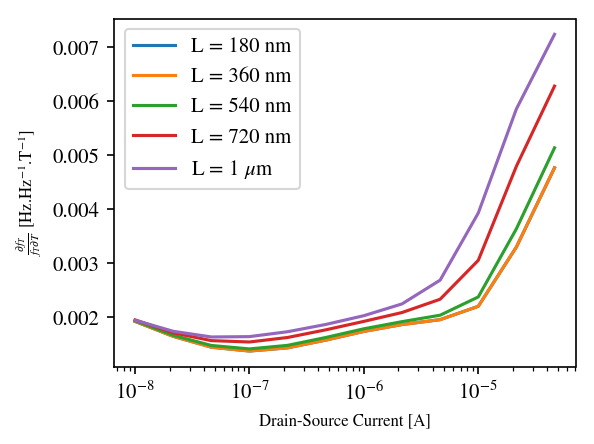
\includegraphics[width=\textwidth]{ft_nel_T}
		\resizebox {\textwidth} {!} {
			%% Creator: Matplotlib, PGF backend
%%
%% To include the figure in your LaTeX document, write
%%   \input{<filename>.pgf}
%%
%% Make sure the required packages are loaded in your preamble
%%   \usepackage{pgf}
%%
%% Figures using additional raster images can only be included by \input if
%% they are in the same directory as the main LaTeX file. For loading figures
%% from other directories you can use the `import` package
%%   \usepackage{import}
%% and then include the figures with
%%   \import{<path to file>}{<filename>.pgf}
%%
%% Matplotlib used the following preamble
%%   \usepackage{gensymb}
%%   \usepackage[utf8x]{inputenc}
%%   \usepackage[T1]{fontenc}
%%
\begingroup%
\makeatletter%
\begin{pgfpicture}%
\pgfpathrectangle{\pgfpointorigin}{\pgfqpoint{3.840000in}{2.840000in}}%
\pgfusepath{use as bounding box, clip}%
\begin{pgfscope}%
\pgfsetbuttcap%
\pgfsetmiterjoin%
\definecolor{currentfill}{rgb}{1.000000,1.000000,1.000000}%
\pgfsetfillcolor{currentfill}%
\pgfsetlinewidth{0.000000pt}%
\definecolor{currentstroke}{rgb}{1.000000,1.000000,1.000000}%
\pgfsetstrokecolor{currentstroke}%
\pgfsetdash{}{0pt}%
\pgfpathmoveto{\pgfqpoint{0.000000in}{0.000000in}}%
\pgfpathlineto{\pgfqpoint{3.840000in}{0.000000in}}%
\pgfpathlineto{\pgfqpoint{3.840000in}{2.840000in}}%
\pgfpathlineto{\pgfqpoint{0.000000in}{2.840000in}}%
\pgfpathclose%
\pgfusepath{fill}%
\end{pgfscope}%
\begin{pgfscope}%
\pgfsetbuttcap%
\pgfsetmiterjoin%
\definecolor{currentfill}{rgb}{1.000000,1.000000,1.000000}%
\pgfsetfillcolor{currentfill}%
\pgfsetlinewidth{0.000000pt}%
\definecolor{currentstroke}{rgb}{0.000000,0.000000,0.000000}%
\pgfsetstrokecolor{currentstroke}%
\pgfsetstrokeopacity{0.000000}%
\pgfsetdash{}{0pt}%
\pgfpathmoveto{\pgfqpoint{1.074061in}{0.596026in}}%
\pgfpathlineto{\pgfqpoint{3.716667in}{0.596026in}}%
\pgfpathlineto{\pgfqpoint{3.716667in}{2.716667in}}%
\pgfpathlineto{\pgfqpoint{1.074061in}{2.716667in}}%
\pgfpathclose%
\pgfusepath{fill}%
\end{pgfscope}%
\begin{pgfscope}%
\pgfsetbuttcap%
\pgfsetroundjoin%
\definecolor{currentfill}{rgb}{0.000000,0.000000,0.000000}%
\pgfsetfillcolor{currentfill}%
\pgfsetlinewidth{0.803000pt}%
\definecolor{currentstroke}{rgb}{0.000000,0.000000,0.000000}%
\pgfsetstrokecolor{currentstroke}%
\pgfsetdash{}{0pt}%
\pgfsys@defobject{currentmarker}{\pgfqpoint{0.000000in}{-0.048611in}}{\pgfqpoint{0.000000in}{0.000000in}}{%
\pgfpathmoveto{\pgfqpoint{0.000000in}{0.000000in}}%
\pgfpathlineto{\pgfqpoint{0.000000in}{-0.048611in}}%
\pgfusepath{stroke,fill}%
}%
\begin{pgfscope}%
\pgfsys@transformshift{1.194179in}{0.596026in}%
\pgfsys@useobject{currentmarker}{}%
\end{pgfscope}%
\end{pgfscope}%
\begin{pgfscope}%
\pgftext[x=1.194179in,y=0.498804in,,top]{\fontsize{14.000000}{16.800000}\selectfont \(\displaystyle 10^{-8}\)}%
\end{pgfscope}%
\begin{pgfscope}%
\pgfsetbuttcap%
\pgfsetroundjoin%
\definecolor{currentfill}{rgb}{0.000000,0.000000,0.000000}%
\pgfsetfillcolor{currentfill}%
\pgfsetlinewidth{0.803000pt}%
\definecolor{currentstroke}{rgb}{0.000000,0.000000,0.000000}%
\pgfsetstrokecolor{currentstroke}%
\pgfsetdash{}{0pt}%
\pgfsys@defobject{currentmarker}{\pgfqpoint{0.000000in}{-0.048611in}}{\pgfqpoint{0.000000in}{0.000000in}}{%
\pgfpathmoveto{\pgfqpoint{0.000000in}{0.000000in}}%
\pgfpathlineto{\pgfqpoint{0.000000in}{-0.048611in}}%
\pgfusepath{stroke,fill}%
}%
\begin{pgfscope}%
\pgfsys@transformshift{1.849364in}{0.596026in}%
\pgfsys@useobject{currentmarker}{}%
\end{pgfscope}%
\end{pgfscope}%
\begin{pgfscope}%
\pgftext[x=1.849364in,y=0.498804in,,top]{\fontsize{14.000000}{16.800000}\selectfont \(\displaystyle 10^{-7}\)}%
\end{pgfscope}%
\begin{pgfscope}%
\pgfsetbuttcap%
\pgfsetroundjoin%
\definecolor{currentfill}{rgb}{0.000000,0.000000,0.000000}%
\pgfsetfillcolor{currentfill}%
\pgfsetlinewidth{0.803000pt}%
\definecolor{currentstroke}{rgb}{0.000000,0.000000,0.000000}%
\pgfsetstrokecolor{currentstroke}%
\pgfsetdash{}{0pt}%
\pgfsys@defobject{currentmarker}{\pgfqpoint{0.000000in}{-0.048611in}}{\pgfqpoint{0.000000in}{0.000000in}}{%
\pgfpathmoveto{\pgfqpoint{0.000000in}{0.000000in}}%
\pgfpathlineto{\pgfqpoint{0.000000in}{-0.048611in}}%
\pgfusepath{stroke,fill}%
}%
\begin{pgfscope}%
\pgfsys@transformshift{2.504549in}{0.596026in}%
\pgfsys@useobject{currentmarker}{}%
\end{pgfscope}%
\end{pgfscope}%
\begin{pgfscope}%
\pgftext[x=2.504549in,y=0.498804in,,top]{\fontsize{14.000000}{16.800000}\selectfont \(\displaystyle 10^{-6}\)}%
\end{pgfscope}%
\begin{pgfscope}%
\pgfsetbuttcap%
\pgfsetroundjoin%
\definecolor{currentfill}{rgb}{0.000000,0.000000,0.000000}%
\pgfsetfillcolor{currentfill}%
\pgfsetlinewidth{0.803000pt}%
\definecolor{currentstroke}{rgb}{0.000000,0.000000,0.000000}%
\pgfsetstrokecolor{currentstroke}%
\pgfsetdash{}{0pt}%
\pgfsys@defobject{currentmarker}{\pgfqpoint{0.000000in}{-0.048611in}}{\pgfqpoint{0.000000in}{0.000000in}}{%
\pgfpathmoveto{\pgfqpoint{0.000000in}{0.000000in}}%
\pgfpathlineto{\pgfqpoint{0.000000in}{-0.048611in}}%
\pgfusepath{stroke,fill}%
}%
\begin{pgfscope}%
\pgfsys@transformshift{3.159733in}{0.596026in}%
\pgfsys@useobject{currentmarker}{}%
\end{pgfscope}%
\end{pgfscope}%
\begin{pgfscope}%
\pgftext[x=3.159733in,y=0.498804in,,top]{\fontsize{14.000000}{16.800000}\selectfont \(\displaystyle 10^{-5}\)}%
\end{pgfscope}%
\begin{pgfscope}%
\pgfsetbuttcap%
\pgfsetroundjoin%
\definecolor{currentfill}{rgb}{0.000000,0.000000,0.000000}%
\pgfsetfillcolor{currentfill}%
\pgfsetlinewidth{0.602250pt}%
\definecolor{currentstroke}{rgb}{0.000000,0.000000,0.000000}%
\pgfsetstrokecolor{currentstroke}%
\pgfsetdash{}{0pt}%
\pgfsys@defobject{currentmarker}{\pgfqpoint{0.000000in}{-0.027778in}}{\pgfqpoint{0.000000in}{0.000000in}}{%
\pgfpathmoveto{\pgfqpoint{0.000000in}{0.000000in}}%
\pgfpathlineto{\pgfqpoint{0.000000in}{-0.027778in}}%
\pgfusepath{stroke,fill}%
}%
\begin{pgfscope}%
\pgfsys@transformshift{1.092690in}{0.596026in}%
\pgfsys@useobject{currentmarker}{}%
\end{pgfscope}%
\end{pgfscope}%
\begin{pgfscope}%
\pgfsetbuttcap%
\pgfsetroundjoin%
\definecolor{currentfill}{rgb}{0.000000,0.000000,0.000000}%
\pgfsetfillcolor{currentfill}%
\pgfsetlinewidth{0.602250pt}%
\definecolor{currentstroke}{rgb}{0.000000,0.000000,0.000000}%
\pgfsetstrokecolor{currentstroke}%
\pgfsetdash{}{0pt}%
\pgfsys@defobject{currentmarker}{\pgfqpoint{0.000000in}{-0.027778in}}{\pgfqpoint{0.000000in}{0.000000in}}{%
\pgfpathmoveto{\pgfqpoint{0.000000in}{0.000000in}}%
\pgfpathlineto{\pgfqpoint{0.000000in}{-0.027778in}}%
\pgfusepath{stroke,fill}%
}%
\begin{pgfscope}%
\pgfsys@transformshift{1.130685in}{0.596026in}%
\pgfsys@useobject{currentmarker}{}%
\end{pgfscope}%
\end{pgfscope}%
\begin{pgfscope}%
\pgfsetbuttcap%
\pgfsetroundjoin%
\definecolor{currentfill}{rgb}{0.000000,0.000000,0.000000}%
\pgfsetfillcolor{currentfill}%
\pgfsetlinewidth{0.602250pt}%
\definecolor{currentstroke}{rgb}{0.000000,0.000000,0.000000}%
\pgfsetstrokecolor{currentstroke}%
\pgfsetdash{}{0pt}%
\pgfsys@defobject{currentmarker}{\pgfqpoint{0.000000in}{-0.027778in}}{\pgfqpoint{0.000000in}{0.000000in}}{%
\pgfpathmoveto{\pgfqpoint{0.000000in}{0.000000in}}%
\pgfpathlineto{\pgfqpoint{0.000000in}{-0.027778in}}%
\pgfusepath{stroke,fill}%
}%
\begin{pgfscope}%
\pgfsys@transformshift{1.164200in}{0.596026in}%
\pgfsys@useobject{currentmarker}{}%
\end{pgfscope}%
\end{pgfscope}%
\begin{pgfscope}%
\pgfsetbuttcap%
\pgfsetroundjoin%
\definecolor{currentfill}{rgb}{0.000000,0.000000,0.000000}%
\pgfsetfillcolor{currentfill}%
\pgfsetlinewidth{0.602250pt}%
\definecolor{currentstroke}{rgb}{0.000000,0.000000,0.000000}%
\pgfsetstrokecolor{currentstroke}%
\pgfsetdash{}{0pt}%
\pgfsys@defobject{currentmarker}{\pgfqpoint{0.000000in}{-0.027778in}}{\pgfqpoint{0.000000in}{0.000000in}}{%
\pgfpathmoveto{\pgfqpoint{0.000000in}{0.000000in}}%
\pgfpathlineto{\pgfqpoint{0.000000in}{-0.027778in}}%
\pgfusepath{stroke,fill}%
}%
\begin{pgfscope}%
\pgfsys@transformshift{1.391410in}{0.596026in}%
\pgfsys@useobject{currentmarker}{}%
\end{pgfscope}%
\end{pgfscope}%
\begin{pgfscope}%
\pgfsetbuttcap%
\pgfsetroundjoin%
\definecolor{currentfill}{rgb}{0.000000,0.000000,0.000000}%
\pgfsetfillcolor{currentfill}%
\pgfsetlinewidth{0.602250pt}%
\definecolor{currentstroke}{rgb}{0.000000,0.000000,0.000000}%
\pgfsetstrokecolor{currentstroke}%
\pgfsetdash{}{0pt}%
\pgfsys@defobject{currentmarker}{\pgfqpoint{0.000000in}{-0.027778in}}{\pgfqpoint{0.000000in}{0.000000in}}{%
\pgfpathmoveto{\pgfqpoint{0.000000in}{0.000000in}}%
\pgfpathlineto{\pgfqpoint{0.000000in}{-0.027778in}}%
\pgfusepath{stroke,fill}%
}%
\begin{pgfscope}%
\pgfsys@transformshift{1.506782in}{0.596026in}%
\pgfsys@useobject{currentmarker}{}%
\end{pgfscope}%
\end{pgfscope}%
\begin{pgfscope}%
\pgfsetbuttcap%
\pgfsetroundjoin%
\definecolor{currentfill}{rgb}{0.000000,0.000000,0.000000}%
\pgfsetfillcolor{currentfill}%
\pgfsetlinewidth{0.602250pt}%
\definecolor{currentstroke}{rgb}{0.000000,0.000000,0.000000}%
\pgfsetstrokecolor{currentstroke}%
\pgfsetdash{}{0pt}%
\pgfsys@defobject{currentmarker}{\pgfqpoint{0.000000in}{-0.027778in}}{\pgfqpoint{0.000000in}{0.000000in}}{%
\pgfpathmoveto{\pgfqpoint{0.000000in}{0.000000in}}%
\pgfpathlineto{\pgfqpoint{0.000000in}{-0.027778in}}%
\pgfusepath{stroke,fill}%
}%
\begin{pgfscope}%
\pgfsys@transformshift{1.588640in}{0.596026in}%
\pgfsys@useobject{currentmarker}{}%
\end{pgfscope}%
\end{pgfscope}%
\begin{pgfscope}%
\pgfsetbuttcap%
\pgfsetroundjoin%
\definecolor{currentfill}{rgb}{0.000000,0.000000,0.000000}%
\pgfsetfillcolor{currentfill}%
\pgfsetlinewidth{0.602250pt}%
\definecolor{currentstroke}{rgb}{0.000000,0.000000,0.000000}%
\pgfsetstrokecolor{currentstroke}%
\pgfsetdash{}{0pt}%
\pgfsys@defobject{currentmarker}{\pgfqpoint{0.000000in}{-0.027778in}}{\pgfqpoint{0.000000in}{0.000000in}}{%
\pgfpathmoveto{\pgfqpoint{0.000000in}{0.000000in}}%
\pgfpathlineto{\pgfqpoint{0.000000in}{-0.027778in}}%
\pgfusepath{stroke,fill}%
}%
\begin{pgfscope}%
\pgfsys@transformshift{1.652134in}{0.596026in}%
\pgfsys@useobject{currentmarker}{}%
\end{pgfscope}%
\end{pgfscope}%
\begin{pgfscope}%
\pgfsetbuttcap%
\pgfsetroundjoin%
\definecolor{currentfill}{rgb}{0.000000,0.000000,0.000000}%
\pgfsetfillcolor{currentfill}%
\pgfsetlinewidth{0.602250pt}%
\definecolor{currentstroke}{rgb}{0.000000,0.000000,0.000000}%
\pgfsetstrokecolor{currentstroke}%
\pgfsetdash{}{0pt}%
\pgfsys@defobject{currentmarker}{\pgfqpoint{0.000000in}{-0.027778in}}{\pgfqpoint{0.000000in}{0.000000in}}{%
\pgfpathmoveto{\pgfqpoint{0.000000in}{0.000000in}}%
\pgfpathlineto{\pgfqpoint{0.000000in}{-0.027778in}}%
\pgfusepath{stroke,fill}%
}%
\begin{pgfscope}%
\pgfsys@transformshift{1.704012in}{0.596026in}%
\pgfsys@useobject{currentmarker}{}%
\end{pgfscope}%
\end{pgfscope}%
\begin{pgfscope}%
\pgfsetbuttcap%
\pgfsetroundjoin%
\definecolor{currentfill}{rgb}{0.000000,0.000000,0.000000}%
\pgfsetfillcolor{currentfill}%
\pgfsetlinewidth{0.602250pt}%
\definecolor{currentstroke}{rgb}{0.000000,0.000000,0.000000}%
\pgfsetstrokecolor{currentstroke}%
\pgfsetdash{}{0pt}%
\pgfsys@defobject{currentmarker}{\pgfqpoint{0.000000in}{-0.027778in}}{\pgfqpoint{0.000000in}{0.000000in}}{%
\pgfpathmoveto{\pgfqpoint{0.000000in}{0.000000in}}%
\pgfpathlineto{\pgfqpoint{0.000000in}{-0.027778in}}%
\pgfusepath{stroke,fill}%
}%
\begin{pgfscope}%
\pgfsys@transformshift{1.747875in}{0.596026in}%
\pgfsys@useobject{currentmarker}{}%
\end{pgfscope}%
\end{pgfscope}%
\begin{pgfscope}%
\pgfsetbuttcap%
\pgfsetroundjoin%
\definecolor{currentfill}{rgb}{0.000000,0.000000,0.000000}%
\pgfsetfillcolor{currentfill}%
\pgfsetlinewidth{0.602250pt}%
\definecolor{currentstroke}{rgb}{0.000000,0.000000,0.000000}%
\pgfsetstrokecolor{currentstroke}%
\pgfsetdash{}{0pt}%
\pgfsys@defobject{currentmarker}{\pgfqpoint{0.000000in}{-0.027778in}}{\pgfqpoint{0.000000in}{0.000000in}}{%
\pgfpathmoveto{\pgfqpoint{0.000000in}{0.000000in}}%
\pgfpathlineto{\pgfqpoint{0.000000in}{-0.027778in}}%
\pgfusepath{stroke,fill}%
}%
\begin{pgfscope}%
\pgfsys@transformshift{1.785870in}{0.596026in}%
\pgfsys@useobject{currentmarker}{}%
\end{pgfscope}%
\end{pgfscope}%
\begin{pgfscope}%
\pgfsetbuttcap%
\pgfsetroundjoin%
\definecolor{currentfill}{rgb}{0.000000,0.000000,0.000000}%
\pgfsetfillcolor{currentfill}%
\pgfsetlinewidth{0.602250pt}%
\definecolor{currentstroke}{rgb}{0.000000,0.000000,0.000000}%
\pgfsetstrokecolor{currentstroke}%
\pgfsetdash{}{0pt}%
\pgfsys@defobject{currentmarker}{\pgfqpoint{0.000000in}{-0.027778in}}{\pgfqpoint{0.000000in}{0.000000in}}{%
\pgfpathmoveto{\pgfqpoint{0.000000in}{0.000000in}}%
\pgfpathlineto{\pgfqpoint{0.000000in}{-0.027778in}}%
\pgfusepath{stroke,fill}%
}%
\begin{pgfscope}%
\pgfsys@transformshift{1.819384in}{0.596026in}%
\pgfsys@useobject{currentmarker}{}%
\end{pgfscope}%
\end{pgfscope}%
\begin{pgfscope}%
\pgfsetbuttcap%
\pgfsetroundjoin%
\definecolor{currentfill}{rgb}{0.000000,0.000000,0.000000}%
\pgfsetfillcolor{currentfill}%
\pgfsetlinewidth{0.602250pt}%
\definecolor{currentstroke}{rgb}{0.000000,0.000000,0.000000}%
\pgfsetstrokecolor{currentstroke}%
\pgfsetdash{}{0pt}%
\pgfsys@defobject{currentmarker}{\pgfqpoint{0.000000in}{-0.027778in}}{\pgfqpoint{0.000000in}{0.000000in}}{%
\pgfpathmoveto{\pgfqpoint{0.000000in}{0.000000in}}%
\pgfpathlineto{\pgfqpoint{0.000000in}{-0.027778in}}%
\pgfusepath{stroke,fill}%
}%
\begin{pgfscope}%
\pgfsys@transformshift{2.046594in}{0.596026in}%
\pgfsys@useobject{currentmarker}{}%
\end{pgfscope}%
\end{pgfscope}%
\begin{pgfscope}%
\pgfsetbuttcap%
\pgfsetroundjoin%
\definecolor{currentfill}{rgb}{0.000000,0.000000,0.000000}%
\pgfsetfillcolor{currentfill}%
\pgfsetlinewidth{0.602250pt}%
\definecolor{currentstroke}{rgb}{0.000000,0.000000,0.000000}%
\pgfsetstrokecolor{currentstroke}%
\pgfsetdash{}{0pt}%
\pgfsys@defobject{currentmarker}{\pgfqpoint{0.000000in}{-0.027778in}}{\pgfqpoint{0.000000in}{0.000000in}}{%
\pgfpathmoveto{\pgfqpoint{0.000000in}{0.000000in}}%
\pgfpathlineto{\pgfqpoint{0.000000in}{-0.027778in}}%
\pgfusepath{stroke,fill}%
}%
\begin{pgfscope}%
\pgfsys@transformshift{2.161967in}{0.596026in}%
\pgfsys@useobject{currentmarker}{}%
\end{pgfscope}%
\end{pgfscope}%
\begin{pgfscope}%
\pgfsetbuttcap%
\pgfsetroundjoin%
\definecolor{currentfill}{rgb}{0.000000,0.000000,0.000000}%
\pgfsetfillcolor{currentfill}%
\pgfsetlinewidth{0.602250pt}%
\definecolor{currentstroke}{rgb}{0.000000,0.000000,0.000000}%
\pgfsetstrokecolor{currentstroke}%
\pgfsetdash{}{0pt}%
\pgfsys@defobject{currentmarker}{\pgfqpoint{0.000000in}{-0.027778in}}{\pgfqpoint{0.000000in}{0.000000in}}{%
\pgfpathmoveto{\pgfqpoint{0.000000in}{0.000000in}}%
\pgfpathlineto{\pgfqpoint{0.000000in}{-0.027778in}}%
\pgfusepath{stroke,fill}%
}%
\begin{pgfscope}%
\pgfsys@transformshift{2.243824in}{0.596026in}%
\pgfsys@useobject{currentmarker}{}%
\end{pgfscope}%
\end{pgfscope}%
\begin{pgfscope}%
\pgfsetbuttcap%
\pgfsetroundjoin%
\definecolor{currentfill}{rgb}{0.000000,0.000000,0.000000}%
\pgfsetfillcolor{currentfill}%
\pgfsetlinewidth{0.602250pt}%
\definecolor{currentstroke}{rgb}{0.000000,0.000000,0.000000}%
\pgfsetstrokecolor{currentstroke}%
\pgfsetdash{}{0pt}%
\pgfsys@defobject{currentmarker}{\pgfqpoint{0.000000in}{-0.027778in}}{\pgfqpoint{0.000000in}{0.000000in}}{%
\pgfpathmoveto{\pgfqpoint{0.000000in}{0.000000in}}%
\pgfpathlineto{\pgfqpoint{0.000000in}{-0.027778in}}%
\pgfusepath{stroke,fill}%
}%
\begin{pgfscope}%
\pgfsys@transformshift{2.307318in}{0.596026in}%
\pgfsys@useobject{currentmarker}{}%
\end{pgfscope}%
\end{pgfscope}%
\begin{pgfscope}%
\pgfsetbuttcap%
\pgfsetroundjoin%
\definecolor{currentfill}{rgb}{0.000000,0.000000,0.000000}%
\pgfsetfillcolor{currentfill}%
\pgfsetlinewidth{0.602250pt}%
\definecolor{currentstroke}{rgb}{0.000000,0.000000,0.000000}%
\pgfsetstrokecolor{currentstroke}%
\pgfsetdash{}{0pt}%
\pgfsys@defobject{currentmarker}{\pgfqpoint{0.000000in}{-0.027778in}}{\pgfqpoint{0.000000in}{0.000000in}}{%
\pgfpathmoveto{\pgfqpoint{0.000000in}{0.000000in}}%
\pgfpathlineto{\pgfqpoint{0.000000in}{-0.027778in}}%
\pgfusepath{stroke,fill}%
}%
\begin{pgfscope}%
\pgfsys@transformshift{2.359197in}{0.596026in}%
\pgfsys@useobject{currentmarker}{}%
\end{pgfscope}%
\end{pgfscope}%
\begin{pgfscope}%
\pgfsetbuttcap%
\pgfsetroundjoin%
\definecolor{currentfill}{rgb}{0.000000,0.000000,0.000000}%
\pgfsetfillcolor{currentfill}%
\pgfsetlinewidth{0.602250pt}%
\definecolor{currentstroke}{rgb}{0.000000,0.000000,0.000000}%
\pgfsetstrokecolor{currentstroke}%
\pgfsetdash{}{0pt}%
\pgfsys@defobject{currentmarker}{\pgfqpoint{0.000000in}{-0.027778in}}{\pgfqpoint{0.000000in}{0.000000in}}{%
\pgfpathmoveto{\pgfqpoint{0.000000in}{0.000000in}}%
\pgfpathlineto{\pgfqpoint{0.000000in}{-0.027778in}}%
\pgfusepath{stroke,fill}%
}%
\begin{pgfscope}%
\pgfsys@transformshift{2.403059in}{0.596026in}%
\pgfsys@useobject{currentmarker}{}%
\end{pgfscope}%
\end{pgfscope}%
\begin{pgfscope}%
\pgfsetbuttcap%
\pgfsetroundjoin%
\definecolor{currentfill}{rgb}{0.000000,0.000000,0.000000}%
\pgfsetfillcolor{currentfill}%
\pgfsetlinewidth{0.602250pt}%
\definecolor{currentstroke}{rgb}{0.000000,0.000000,0.000000}%
\pgfsetstrokecolor{currentstroke}%
\pgfsetdash{}{0pt}%
\pgfsys@defobject{currentmarker}{\pgfqpoint{0.000000in}{-0.027778in}}{\pgfqpoint{0.000000in}{0.000000in}}{%
\pgfpathmoveto{\pgfqpoint{0.000000in}{0.000000in}}%
\pgfpathlineto{\pgfqpoint{0.000000in}{-0.027778in}}%
\pgfusepath{stroke,fill}%
}%
\begin{pgfscope}%
\pgfsys@transformshift{2.441055in}{0.596026in}%
\pgfsys@useobject{currentmarker}{}%
\end{pgfscope}%
\end{pgfscope}%
\begin{pgfscope}%
\pgfsetbuttcap%
\pgfsetroundjoin%
\definecolor{currentfill}{rgb}{0.000000,0.000000,0.000000}%
\pgfsetfillcolor{currentfill}%
\pgfsetlinewidth{0.602250pt}%
\definecolor{currentstroke}{rgb}{0.000000,0.000000,0.000000}%
\pgfsetstrokecolor{currentstroke}%
\pgfsetdash{}{0pt}%
\pgfsys@defobject{currentmarker}{\pgfqpoint{0.000000in}{-0.027778in}}{\pgfqpoint{0.000000in}{0.000000in}}{%
\pgfpathmoveto{\pgfqpoint{0.000000in}{0.000000in}}%
\pgfpathlineto{\pgfqpoint{0.000000in}{-0.027778in}}%
\pgfusepath{stroke,fill}%
}%
\begin{pgfscope}%
\pgfsys@transformshift{2.474569in}{0.596026in}%
\pgfsys@useobject{currentmarker}{}%
\end{pgfscope}%
\end{pgfscope}%
\begin{pgfscope}%
\pgfsetbuttcap%
\pgfsetroundjoin%
\definecolor{currentfill}{rgb}{0.000000,0.000000,0.000000}%
\pgfsetfillcolor{currentfill}%
\pgfsetlinewidth{0.602250pt}%
\definecolor{currentstroke}{rgb}{0.000000,0.000000,0.000000}%
\pgfsetstrokecolor{currentstroke}%
\pgfsetdash{}{0pt}%
\pgfsys@defobject{currentmarker}{\pgfqpoint{0.000000in}{-0.027778in}}{\pgfqpoint{0.000000in}{0.000000in}}{%
\pgfpathmoveto{\pgfqpoint{0.000000in}{0.000000in}}%
\pgfpathlineto{\pgfqpoint{0.000000in}{-0.027778in}}%
\pgfusepath{stroke,fill}%
}%
\begin{pgfscope}%
\pgfsys@transformshift{2.701779in}{0.596026in}%
\pgfsys@useobject{currentmarker}{}%
\end{pgfscope}%
\end{pgfscope}%
\begin{pgfscope}%
\pgfsetbuttcap%
\pgfsetroundjoin%
\definecolor{currentfill}{rgb}{0.000000,0.000000,0.000000}%
\pgfsetfillcolor{currentfill}%
\pgfsetlinewidth{0.602250pt}%
\definecolor{currentstroke}{rgb}{0.000000,0.000000,0.000000}%
\pgfsetstrokecolor{currentstroke}%
\pgfsetdash{}{0pt}%
\pgfsys@defobject{currentmarker}{\pgfqpoint{0.000000in}{-0.027778in}}{\pgfqpoint{0.000000in}{0.000000in}}{%
\pgfpathmoveto{\pgfqpoint{0.000000in}{0.000000in}}%
\pgfpathlineto{\pgfqpoint{0.000000in}{-0.027778in}}%
\pgfusepath{stroke,fill}%
}%
\begin{pgfscope}%
\pgfsys@transformshift{2.817151in}{0.596026in}%
\pgfsys@useobject{currentmarker}{}%
\end{pgfscope}%
\end{pgfscope}%
\begin{pgfscope}%
\pgfsetbuttcap%
\pgfsetroundjoin%
\definecolor{currentfill}{rgb}{0.000000,0.000000,0.000000}%
\pgfsetfillcolor{currentfill}%
\pgfsetlinewidth{0.602250pt}%
\definecolor{currentstroke}{rgb}{0.000000,0.000000,0.000000}%
\pgfsetstrokecolor{currentstroke}%
\pgfsetdash{}{0pt}%
\pgfsys@defobject{currentmarker}{\pgfqpoint{0.000000in}{-0.027778in}}{\pgfqpoint{0.000000in}{0.000000in}}{%
\pgfpathmoveto{\pgfqpoint{0.000000in}{0.000000in}}%
\pgfpathlineto{\pgfqpoint{0.000000in}{-0.027778in}}%
\pgfusepath{stroke,fill}%
}%
\begin{pgfscope}%
\pgfsys@transformshift{2.899009in}{0.596026in}%
\pgfsys@useobject{currentmarker}{}%
\end{pgfscope}%
\end{pgfscope}%
\begin{pgfscope}%
\pgfsetbuttcap%
\pgfsetroundjoin%
\definecolor{currentfill}{rgb}{0.000000,0.000000,0.000000}%
\pgfsetfillcolor{currentfill}%
\pgfsetlinewidth{0.602250pt}%
\definecolor{currentstroke}{rgb}{0.000000,0.000000,0.000000}%
\pgfsetstrokecolor{currentstroke}%
\pgfsetdash{}{0pt}%
\pgfsys@defobject{currentmarker}{\pgfqpoint{0.000000in}{-0.027778in}}{\pgfqpoint{0.000000in}{0.000000in}}{%
\pgfpathmoveto{\pgfqpoint{0.000000in}{0.000000in}}%
\pgfpathlineto{\pgfqpoint{0.000000in}{-0.027778in}}%
\pgfusepath{stroke,fill}%
}%
\begin{pgfscope}%
\pgfsys@transformshift{2.962503in}{0.596026in}%
\pgfsys@useobject{currentmarker}{}%
\end{pgfscope}%
\end{pgfscope}%
\begin{pgfscope}%
\pgfsetbuttcap%
\pgfsetroundjoin%
\definecolor{currentfill}{rgb}{0.000000,0.000000,0.000000}%
\pgfsetfillcolor{currentfill}%
\pgfsetlinewidth{0.602250pt}%
\definecolor{currentstroke}{rgb}{0.000000,0.000000,0.000000}%
\pgfsetstrokecolor{currentstroke}%
\pgfsetdash{}{0pt}%
\pgfsys@defobject{currentmarker}{\pgfqpoint{0.000000in}{-0.027778in}}{\pgfqpoint{0.000000in}{0.000000in}}{%
\pgfpathmoveto{\pgfqpoint{0.000000in}{0.000000in}}%
\pgfpathlineto{\pgfqpoint{0.000000in}{-0.027778in}}%
\pgfusepath{stroke,fill}%
}%
\begin{pgfscope}%
\pgfsys@transformshift{3.014381in}{0.596026in}%
\pgfsys@useobject{currentmarker}{}%
\end{pgfscope}%
\end{pgfscope}%
\begin{pgfscope}%
\pgfsetbuttcap%
\pgfsetroundjoin%
\definecolor{currentfill}{rgb}{0.000000,0.000000,0.000000}%
\pgfsetfillcolor{currentfill}%
\pgfsetlinewidth{0.602250pt}%
\definecolor{currentstroke}{rgb}{0.000000,0.000000,0.000000}%
\pgfsetstrokecolor{currentstroke}%
\pgfsetdash{}{0pt}%
\pgfsys@defobject{currentmarker}{\pgfqpoint{0.000000in}{-0.027778in}}{\pgfqpoint{0.000000in}{0.000000in}}{%
\pgfpathmoveto{\pgfqpoint{0.000000in}{0.000000in}}%
\pgfpathlineto{\pgfqpoint{0.000000in}{-0.027778in}}%
\pgfusepath{stroke,fill}%
}%
\begin{pgfscope}%
\pgfsys@transformshift{3.058244in}{0.596026in}%
\pgfsys@useobject{currentmarker}{}%
\end{pgfscope}%
\end{pgfscope}%
\begin{pgfscope}%
\pgfsetbuttcap%
\pgfsetroundjoin%
\definecolor{currentfill}{rgb}{0.000000,0.000000,0.000000}%
\pgfsetfillcolor{currentfill}%
\pgfsetlinewidth{0.602250pt}%
\definecolor{currentstroke}{rgb}{0.000000,0.000000,0.000000}%
\pgfsetstrokecolor{currentstroke}%
\pgfsetdash{}{0pt}%
\pgfsys@defobject{currentmarker}{\pgfqpoint{0.000000in}{-0.027778in}}{\pgfqpoint{0.000000in}{0.000000in}}{%
\pgfpathmoveto{\pgfqpoint{0.000000in}{0.000000in}}%
\pgfpathlineto{\pgfqpoint{0.000000in}{-0.027778in}}%
\pgfusepath{stroke,fill}%
}%
\begin{pgfscope}%
\pgfsys@transformshift{3.096239in}{0.596026in}%
\pgfsys@useobject{currentmarker}{}%
\end{pgfscope}%
\end{pgfscope}%
\begin{pgfscope}%
\pgfsetbuttcap%
\pgfsetroundjoin%
\definecolor{currentfill}{rgb}{0.000000,0.000000,0.000000}%
\pgfsetfillcolor{currentfill}%
\pgfsetlinewidth{0.602250pt}%
\definecolor{currentstroke}{rgb}{0.000000,0.000000,0.000000}%
\pgfsetstrokecolor{currentstroke}%
\pgfsetdash{}{0pt}%
\pgfsys@defobject{currentmarker}{\pgfqpoint{0.000000in}{-0.027778in}}{\pgfqpoint{0.000000in}{0.000000in}}{%
\pgfpathmoveto{\pgfqpoint{0.000000in}{0.000000in}}%
\pgfpathlineto{\pgfqpoint{0.000000in}{-0.027778in}}%
\pgfusepath{stroke,fill}%
}%
\begin{pgfscope}%
\pgfsys@transformshift{3.129754in}{0.596026in}%
\pgfsys@useobject{currentmarker}{}%
\end{pgfscope}%
\end{pgfscope}%
\begin{pgfscope}%
\pgfsetbuttcap%
\pgfsetroundjoin%
\definecolor{currentfill}{rgb}{0.000000,0.000000,0.000000}%
\pgfsetfillcolor{currentfill}%
\pgfsetlinewidth{0.602250pt}%
\definecolor{currentstroke}{rgb}{0.000000,0.000000,0.000000}%
\pgfsetstrokecolor{currentstroke}%
\pgfsetdash{}{0pt}%
\pgfsys@defobject{currentmarker}{\pgfqpoint{0.000000in}{-0.027778in}}{\pgfqpoint{0.000000in}{0.000000in}}{%
\pgfpathmoveto{\pgfqpoint{0.000000in}{0.000000in}}%
\pgfpathlineto{\pgfqpoint{0.000000in}{-0.027778in}}%
\pgfusepath{stroke,fill}%
}%
\begin{pgfscope}%
\pgfsys@transformshift{3.356963in}{0.596026in}%
\pgfsys@useobject{currentmarker}{}%
\end{pgfscope}%
\end{pgfscope}%
\begin{pgfscope}%
\pgfsetbuttcap%
\pgfsetroundjoin%
\definecolor{currentfill}{rgb}{0.000000,0.000000,0.000000}%
\pgfsetfillcolor{currentfill}%
\pgfsetlinewidth{0.602250pt}%
\definecolor{currentstroke}{rgb}{0.000000,0.000000,0.000000}%
\pgfsetstrokecolor{currentstroke}%
\pgfsetdash{}{0pt}%
\pgfsys@defobject{currentmarker}{\pgfqpoint{0.000000in}{-0.027778in}}{\pgfqpoint{0.000000in}{0.000000in}}{%
\pgfpathmoveto{\pgfqpoint{0.000000in}{0.000000in}}%
\pgfpathlineto{\pgfqpoint{0.000000in}{-0.027778in}}%
\pgfusepath{stroke,fill}%
}%
\begin{pgfscope}%
\pgfsys@transformshift{3.472336in}{0.596026in}%
\pgfsys@useobject{currentmarker}{}%
\end{pgfscope}%
\end{pgfscope}%
\begin{pgfscope}%
\pgfsetbuttcap%
\pgfsetroundjoin%
\definecolor{currentfill}{rgb}{0.000000,0.000000,0.000000}%
\pgfsetfillcolor{currentfill}%
\pgfsetlinewidth{0.602250pt}%
\definecolor{currentstroke}{rgb}{0.000000,0.000000,0.000000}%
\pgfsetstrokecolor{currentstroke}%
\pgfsetdash{}{0pt}%
\pgfsys@defobject{currentmarker}{\pgfqpoint{0.000000in}{-0.027778in}}{\pgfqpoint{0.000000in}{0.000000in}}{%
\pgfpathmoveto{\pgfqpoint{0.000000in}{0.000000in}}%
\pgfpathlineto{\pgfqpoint{0.000000in}{-0.027778in}}%
\pgfusepath{stroke,fill}%
}%
\begin{pgfscope}%
\pgfsys@transformshift{3.554194in}{0.596026in}%
\pgfsys@useobject{currentmarker}{}%
\end{pgfscope}%
\end{pgfscope}%
\begin{pgfscope}%
\pgfsetbuttcap%
\pgfsetroundjoin%
\definecolor{currentfill}{rgb}{0.000000,0.000000,0.000000}%
\pgfsetfillcolor{currentfill}%
\pgfsetlinewidth{0.602250pt}%
\definecolor{currentstroke}{rgb}{0.000000,0.000000,0.000000}%
\pgfsetstrokecolor{currentstroke}%
\pgfsetdash{}{0pt}%
\pgfsys@defobject{currentmarker}{\pgfqpoint{0.000000in}{-0.027778in}}{\pgfqpoint{0.000000in}{0.000000in}}{%
\pgfpathmoveto{\pgfqpoint{0.000000in}{0.000000in}}%
\pgfpathlineto{\pgfqpoint{0.000000in}{-0.027778in}}%
\pgfusepath{stroke,fill}%
}%
\begin{pgfscope}%
\pgfsys@transformshift{3.617688in}{0.596026in}%
\pgfsys@useobject{currentmarker}{}%
\end{pgfscope}%
\end{pgfscope}%
\begin{pgfscope}%
\pgfsetbuttcap%
\pgfsetroundjoin%
\definecolor{currentfill}{rgb}{0.000000,0.000000,0.000000}%
\pgfsetfillcolor{currentfill}%
\pgfsetlinewidth{0.602250pt}%
\definecolor{currentstroke}{rgb}{0.000000,0.000000,0.000000}%
\pgfsetstrokecolor{currentstroke}%
\pgfsetdash{}{0pt}%
\pgfsys@defobject{currentmarker}{\pgfqpoint{0.000000in}{-0.027778in}}{\pgfqpoint{0.000000in}{0.000000in}}{%
\pgfpathmoveto{\pgfqpoint{0.000000in}{0.000000in}}%
\pgfpathlineto{\pgfqpoint{0.000000in}{-0.027778in}}%
\pgfusepath{stroke,fill}%
}%
\begin{pgfscope}%
\pgfsys@transformshift{3.669566in}{0.596026in}%
\pgfsys@useobject{currentmarker}{}%
\end{pgfscope}%
\end{pgfscope}%
\begin{pgfscope}%
\pgfsetbuttcap%
\pgfsetroundjoin%
\definecolor{currentfill}{rgb}{0.000000,0.000000,0.000000}%
\pgfsetfillcolor{currentfill}%
\pgfsetlinewidth{0.602250pt}%
\definecolor{currentstroke}{rgb}{0.000000,0.000000,0.000000}%
\pgfsetstrokecolor{currentstroke}%
\pgfsetdash{}{0pt}%
\pgfsys@defobject{currentmarker}{\pgfqpoint{0.000000in}{-0.027778in}}{\pgfqpoint{0.000000in}{0.000000in}}{%
\pgfpathmoveto{\pgfqpoint{0.000000in}{0.000000in}}%
\pgfpathlineto{\pgfqpoint{0.000000in}{-0.027778in}}%
\pgfusepath{stroke,fill}%
}%
\begin{pgfscope}%
\pgfsys@transformshift{3.713429in}{0.596026in}%
\pgfsys@useobject{currentmarker}{}%
\end{pgfscope}%
\end{pgfscope}%
\begin{pgfscope}%
\pgftext[x=2.395364in,y=0.266626in,,top]{\fontsize{12.000000}{14.400000}\selectfont Drain-Source Current [A]}%
\end{pgfscope}%
\begin{pgfscope}%
\pgfsetbuttcap%
\pgfsetroundjoin%
\definecolor{currentfill}{rgb}{0.000000,0.000000,0.000000}%
\pgfsetfillcolor{currentfill}%
\pgfsetlinewidth{0.803000pt}%
\definecolor{currentstroke}{rgb}{0.000000,0.000000,0.000000}%
\pgfsetstrokecolor{currentstroke}%
\pgfsetdash{}{0pt}%
\pgfsys@defobject{currentmarker}{\pgfqpoint{-0.048611in}{0.000000in}}{\pgfqpoint{0.000000in}{0.000000in}}{%
\pgfpathmoveto{\pgfqpoint{0.000000in}{0.000000in}}%
\pgfpathlineto{\pgfqpoint{-0.048611in}{0.000000in}}%
\pgfusepath{stroke,fill}%
}%
\begin{pgfscope}%
\pgfsys@transformshift{1.074061in}{0.896669in}%
\pgfsys@useobject{currentmarker}{}%
\end{pgfscope}%
\end{pgfscope}%
\begin{pgfscope}%
\pgftext[x=0.530780in,y=0.827803in,left,base]{\fontsize{14.000000}{16.800000}\selectfont \(\displaystyle 0.002\)}%
\end{pgfscope}%
\begin{pgfscope}%
\pgfsetbuttcap%
\pgfsetroundjoin%
\definecolor{currentfill}{rgb}{0.000000,0.000000,0.000000}%
\pgfsetfillcolor{currentfill}%
\pgfsetlinewidth{0.803000pt}%
\definecolor{currentstroke}{rgb}{0.000000,0.000000,0.000000}%
\pgfsetstrokecolor{currentstroke}%
\pgfsetdash{}{0pt}%
\pgfsys@defobject{currentmarker}{\pgfqpoint{-0.048611in}{0.000000in}}{\pgfqpoint{0.000000in}{0.000000in}}{%
\pgfpathmoveto{\pgfqpoint{0.000000in}{0.000000in}}%
\pgfpathlineto{\pgfqpoint{-0.048611in}{0.000000in}}%
\pgfusepath{stroke,fill}%
}%
\begin{pgfscope}%
\pgfsys@transformshift{1.074061in}{1.554583in}%
\pgfsys@useobject{currentmarker}{}%
\end{pgfscope}%
\end{pgfscope}%
\begin{pgfscope}%
\pgftext[x=0.530780in,y=1.485717in,left,base]{\fontsize{14.000000}{16.800000}\selectfont \(\displaystyle 0.004\)}%
\end{pgfscope}%
\begin{pgfscope}%
\pgfsetbuttcap%
\pgfsetroundjoin%
\definecolor{currentfill}{rgb}{0.000000,0.000000,0.000000}%
\pgfsetfillcolor{currentfill}%
\pgfsetlinewidth{0.803000pt}%
\definecolor{currentstroke}{rgb}{0.000000,0.000000,0.000000}%
\pgfsetstrokecolor{currentstroke}%
\pgfsetdash{}{0pt}%
\pgfsys@defobject{currentmarker}{\pgfqpoint{-0.048611in}{0.000000in}}{\pgfqpoint{0.000000in}{0.000000in}}{%
\pgfpathmoveto{\pgfqpoint{0.000000in}{0.000000in}}%
\pgfpathlineto{\pgfqpoint{-0.048611in}{0.000000in}}%
\pgfusepath{stroke,fill}%
}%
\begin{pgfscope}%
\pgfsys@transformshift{1.074061in}{2.212497in}%
\pgfsys@useobject{currentmarker}{}%
\end{pgfscope}%
\end{pgfscope}%
\begin{pgfscope}%
\pgftext[x=0.530780in,y=2.143631in,left,base]{\fontsize{14.000000}{16.800000}\selectfont \(\displaystyle 0.006\)}%
\end{pgfscope}%
\begin{pgfscope}%
\pgftext[x=0.475224in,y=1.656346in,,bottom,rotate=90.000000]{\fontsize{12.000000}{14.400000}\selectfont \(\displaystyle \frac{\partial f_T}{f_T \partial T}\) [Hz.Hz\(\displaystyle ^{-1}\).T\(\displaystyle ^{-1}\)]}%
\end{pgfscope}%
\begin{pgfscope}%
\pgfpathrectangle{\pgfqpoint{1.074061in}{0.596026in}}{\pgfqpoint{2.642606in}{2.120641in}} %
\pgfusepath{clip}%
\pgfsetrectcap%
\pgfsetroundjoin%
\pgfsetlinewidth{1.505625pt}%
\definecolor{currentstroke}{rgb}{0.121569,0.466667,0.705882}%
\pgfsetstrokecolor{currentstroke}%
\pgfsetdash{}{0pt}%
\pgfpathmoveto{\pgfqpoint{1.194179in}{0.872749in}}%
\pgfpathlineto{\pgfqpoint{1.412517in}{0.781890in}}%
\pgfpathlineto{\pgfqpoint{1.630994in}{0.715786in}}%
\pgfpathlineto{\pgfqpoint{1.849364in}{0.692419in}}%
\pgfpathlineto{\pgfqpoint{2.067701in}{0.711903in}}%
\pgfpathlineto{\pgfqpoint{2.286179in}{0.758948in}}%
\pgfpathlineto{\pgfqpoint{2.504549in}{0.811838in}}%
\pgfpathlineto{\pgfqpoint{2.722886in}{0.853643in}}%
\pgfpathlineto{\pgfqpoint{2.941364in}{0.883407in}}%
\pgfpathlineto{\pgfqpoint{3.159733in}{0.964459in}}%
\pgfpathlineto{\pgfqpoint{3.378071in}{1.325468in}}%
\pgfpathlineto{\pgfqpoint{3.596548in}{1.807753in}}%
\pgfusepath{stroke}%
\end{pgfscope}%
\begin{pgfscope}%
\pgfpathrectangle{\pgfqpoint{1.074061in}{0.596026in}}{\pgfqpoint{2.642606in}{2.120641in}} %
\pgfusepath{clip}%
\pgfsetrectcap%
\pgfsetroundjoin%
\pgfsetlinewidth{1.505625pt}%
\definecolor{currentstroke}{rgb}{1.000000,0.498039,0.054902}%
\pgfsetstrokecolor{currentstroke}%
\pgfsetdash{}{0pt}%
\pgfpathmoveto{\pgfqpoint{1.194179in}{0.872749in}}%
\pgfpathlineto{\pgfqpoint{1.412517in}{0.781890in}}%
\pgfpathlineto{\pgfqpoint{1.630994in}{0.715786in}}%
\pgfpathlineto{\pgfqpoint{1.849364in}{0.692419in}}%
\pgfpathlineto{\pgfqpoint{2.067701in}{0.711903in}}%
\pgfpathlineto{\pgfqpoint{2.286179in}{0.758948in}}%
\pgfpathlineto{\pgfqpoint{2.504549in}{0.811838in}}%
\pgfpathlineto{\pgfqpoint{2.722886in}{0.853643in}}%
\pgfpathlineto{\pgfqpoint{2.941364in}{0.883407in}}%
\pgfpathlineto{\pgfqpoint{3.159733in}{0.964459in}}%
\pgfpathlineto{\pgfqpoint{3.378071in}{1.325468in}}%
\pgfpathlineto{\pgfqpoint{3.596548in}{1.807753in}}%
\pgfusepath{stroke}%
\end{pgfscope}%
\begin{pgfscope}%
\pgfpathrectangle{\pgfqpoint{1.074061in}{0.596026in}}{\pgfqpoint{2.642606in}{2.120641in}} %
\pgfusepath{clip}%
\pgfsetrectcap%
\pgfsetroundjoin%
\pgfsetlinewidth{1.505625pt}%
\definecolor{currentstroke}{rgb}{0.172549,0.627451,0.172549}%
\pgfsetstrokecolor{currentstroke}%
\pgfsetdash{}{0pt}%
\pgfpathmoveto{\pgfqpoint{1.194179in}{0.876672in}}%
\pgfpathlineto{\pgfqpoint{1.412517in}{0.788149in}}%
\pgfpathlineto{\pgfqpoint{1.630994in}{0.726242in}}%
\pgfpathlineto{\pgfqpoint{1.849364in}{0.705341in}}%
\pgfpathlineto{\pgfqpoint{2.067701in}{0.727026in}}%
\pgfpathlineto{\pgfqpoint{2.286179in}{0.774826in}}%
\pgfpathlineto{\pgfqpoint{2.504549in}{0.827863in}}%
\pgfpathlineto{\pgfqpoint{2.722886in}{0.871238in}}%
\pgfpathlineto{\pgfqpoint{2.941364in}{0.910518in}}%
\pgfpathlineto{\pgfqpoint{3.159733in}{1.021700in}}%
\pgfpathlineto{\pgfqpoint{3.378071in}{1.436496in}}%
\pgfpathlineto{\pgfqpoint{3.596548in}{1.929324in}}%
\pgfusepath{stroke}%
\end{pgfscope}%
\begin{pgfscope}%
\pgfpathrectangle{\pgfqpoint{1.074061in}{0.596026in}}{\pgfqpoint{2.642606in}{2.120641in}} %
\pgfusepath{clip}%
\pgfsetrectcap%
\pgfsetroundjoin%
\pgfsetlinewidth{1.505625pt}%
\definecolor{currentstroke}{rgb}{0.839216,0.152941,0.156863}%
\pgfsetstrokecolor{currentstroke}%
\pgfsetdash{}{0pt}%
\pgfpathmoveto{\pgfqpoint{1.194179in}{0.882121in}}%
\pgfpathlineto{\pgfqpoint{1.412517in}{0.803298in}}%
\pgfpathlineto{\pgfqpoint{1.630994in}{0.755700in}}%
\pgfpathlineto{\pgfqpoint{1.849364in}{0.747481in}}%
\pgfpathlineto{\pgfqpoint{2.067701in}{0.774881in}}%
\pgfpathlineto{\pgfqpoint{2.286179in}{0.821437in}}%
\pgfpathlineto{\pgfqpoint{2.504549in}{0.873002in}}%
\pgfpathlineto{\pgfqpoint{2.722886in}{0.926759in}}%
\pgfpathlineto{\pgfqpoint{2.941364in}{1.007744in}}%
\pgfpathlineto{\pgfqpoint{3.159733in}{1.244438in}}%
\pgfpathlineto{\pgfqpoint{3.378071in}{1.817137in}}%
\pgfpathlineto{\pgfqpoint{3.596548in}{2.305100in}}%
\pgfusepath{stroke}%
\end{pgfscope}%
\begin{pgfscope}%
\pgfpathrectangle{\pgfqpoint{1.074061in}{0.596026in}}{\pgfqpoint{2.642606in}{2.120641in}} %
\pgfusepath{clip}%
\pgfsetrectcap%
\pgfsetroundjoin%
\pgfsetlinewidth{1.505625pt}%
\definecolor{currentstroke}{rgb}{0.580392,0.403922,0.741176}%
\pgfsetstrokecolor{currentstroke}%
\pgfsetdash{}{0pt}%
\pgfpathmoveto{\pgfqpoint{1.194179in}{0.879937in}}%
\pgfpathlineto{\pgfqpoint{1.412517in}{0.812547in}}%
\pgfpathlineto{\pgfqpoint{1.630994in}{0.778014in}}%
\pgfpathlineto{\pgfqpoint{1.849364in}{0.780183in}}%
\pgfpathlineto{\pgfqpoint{2.067701in}{0.810012in}}%
\pgfpathlineto{\pgfqpoint{2.286179in}{0.854210in}}%
\pgfpathlineto{\pgfqpoint{2.504549in}{0.907607in}}%
\pgfpathlineto{\pgfqpoint{2.722886in}{0.979172in}}%
\pgfpathlineto{\pgfqpoint{2.941364in}{1.124062in}}%
\pgfpathlineto{\pgfqpoint{3.159733in}{1.532363in}}%
\pgfpathlineto{\pgfqpoint{3.378071in}{2.165967in}}%
\pgfpathlineto{\pgfqpoint{3.596548in}{2.620274in}}%
\pgfusepath{stroke}%
\end{pgfscope}%
\begin{pgfscope}%
\pgfsetrectcap%
\pgfsetmiterjoin%
\pgfsetlinewidth{0.803000pt}%
\definecolor{currentstroke}{rgb}{0.000000,0.000000,0.000000}%
\pgfsetstrokecolor{currentstroke}%
\pgfsetdash{}{0pt}%
\pgfpathmoveto{\pgfqpoint{1.074061in}{0.596026in}}%
\pgfpathlineto{\pgfqpoint{1.074061in}{2.716667in}}%
\pgfusepath{stroke}%
\end{pgfscope}%
\begin{pgfscope}%
\pgfsetrectcap%
\pgfsetmiterjoin%
\pgfsetlinewidth{0.803000pt}%
\definecolor{currentstroke}{rgb}{0.000000,0.000000,0.000000}%
\pgfsetstrokecolor{currentstroke}%
\pgfsetdash{}{0pt}%
\pgfpathmoveto{\pgfqpoint{3.716667in}{0.596026in}}%
\pgfpathlineto{\pgfqpoint{3.716667in}{2.716667in}}%
\pgfusepath{stroke}%
\end{pgfscope}%
\begin{pgfscope}%
\pgfsetrectcap%
\pgfsetmiterjoin%
\pgfsetlinewidth{0.803000pt}%
\definecolor{currentstroke}{rgb}{0.000000,0.000000,0.000000}%
\pgfsetstrokecolor{currentstroke}%
\pgfsetdash{}{0pt}%
\pgfpathmoveto{\pgfqpoint{1.074061in}{0.596026in}}%
\pgfpathlineto{\pgfqpoint{3.716667in}{0.596026in}}%
\pgfusepath{stroke}%
\end{pgfscope}%
\begin{pgfscope}%
\pgfsetrectcap%
\pgfsetmiterjoin%
\pgfsetlinewidth{0.803000pt}%
\definecolor{currentstroke}{rgb}{0.000000,0.000000,0.000000}%
\pgfsetstrokecolor{currentstroke}%
\pgfsetdash{}{0pt}%
\pgfpathmoveto{\pgfqpoint{1.074061in}{2.716667in}}%
\pgfpathlineto{\pgfqpoint{3.716667in}{2.716667in}}%
\pgfusepath{stroke}%
\end{pgfscope}%
\begin{pgfscope}%
\pgfsetbuttcap%
\pgfsetmiterjoin%
\definecolor{currentfill}{rgb}{1.000000,1.000000,1.000000}%
\pgfsetfillcolor{currentfill}%
\pgfsetfillopacity{0.800000}%
\pgfsetlinewidth{1.003750pt}%
\definecolor{currentstroke}{rgb}{0.800000,0.800000,0.800000}%
\pgfsetstrokecolor{currentstroke}%
\pgfsetstrokeopacity{0.800000}%
\pgfsetdash{}{0pt}%
\pgfpathmoveto{\pgfqpoint{1.171283in}{1.637218in}}%
\pgfpathlineto{\pgfqpoint{2.350502in}{1.637218in}}%
\pgfpathquadraticcurveto{\pgfqpoint{2.378280in}{1.637218in}}{\pgfqpoint{2.378280in}{1.664996in}}%
\pgfpathlineto{\pgfqpoint{2.378280in}{2.619444in}}%
\pgfpathquadraticcurveto{\pgfqpoint{2.378280in}{2.647222in}}{\pgfqpoint{2.350502in}{2.647222in}}%
\pgfpathlineto{\pgfqpoint{1.171283in}{2.647222in}}%
\pgfpathquadraticcurveto{\pgfqpoint{1.143505in}{2.647222in}}{\pgfqpoint{1.143505in}{2.619444in}}%
\pgfpathlineto{\pgfqpoint{1.143505in}{1.664996in}}%
\pgfpathquadraticcurveto{\pgfqpoint{1.143505in}{1.637218in}}{\pgfqpoint{1.171283in}{1.637218in}}%
\pgfpathclose%
\pgfusepath{stroke,fill}%
\end{pgfscope}%
\begin{pgfscope}%
\pgfsetrectcap%
\pgfsetroundjoin%
\pgfsetlinewidth{1.505625pt}%
\definecolor{currentstroke}{rgb}{0.121569,0.466667,0.705882}%
\pgfsetstrokecolor{currentstroke}%
\pgfsetdash{}{0pt}%
\pgfpathmoveto{\pgfqpoint{1.199061in}{2.543056in}}%
\pgfpathlineto{\pgfqpoint{1.476839in}{2.543056in}}%
\pgfusepath{stroke}%
\end{pgfscope}%
\begin{pgfscope}%
\pgftext[x=1.587950in,y=2.494444in,left,base]{\fontsize{10.000000}{12.000000}\selectfont L = 180 nm}%
\end{pgfscope}%
\begin{pgfscope}%
\pgfsetrectcap%
\pgfsetroundjoin%
\pgfsetlinewidth{1.505625pt}%
\definecolor{currentstroke}{rgb}{1.000000,0.498039,0.054902}%
\pgfsetstrokecolor{currentstroke}%
\pgfsetdash{}{0pt}%
\pgfpathmoveto{\pgfqpoint{1.199061in}{2.349389in}}%
\pgfpathlineto{\pgfqpoint{1.476839in}{2.349389in}}%
\pgfusepath{stroke}%
\end{pgfscope}%
\begin{pgfscope}%
\pgftext[x=1.587950in,y=2.300778in,left,base]{\fontsize{10.000000}{12.000000}\selectfont L = 360 nm}%
\end{pgfscope}%
\begin{pgfscope}%
\pgfsetrectcap%
\pgfsetroundjoin%
\pgfsetlinewidth{1.505625pt}%
\definecolor{currentstroke}{rgb}{0.172549,0.627451,0.172549}%
\pgfsetstrokecolor{currentstroke}%
\pgfsetdash{}{0pt}%
\pgfpathmoveto{\pgfqpoint{1.199061in}{2.155723in}}%
\pgfpathlineto{\pgfqpoint{1.476839in}{2.155723in}}%
\pgfusepath{stroke}%
\end{pgfscope}%
\begin{pgfscope}%
\pgftext[x=1.587950in,y=2.107112in,left,base]{\fontsize{10.000000}{12.000000}\selectfont L = 540 nm}%
\end{pgfscope}%
\begin{pgfscope}%
\pgfsetrectcap%
\pgfsetroundjoin%
\pgfsetlinewidth{1.505625pt}%
\definecolor{currentstroke}{rgb}{0.839216,0.152941,0.156863}%
\pgfsetstrokecolor{currentstroke}%
\pgfsetdash{}{0pt}%
\pgfpathmoveto{\pgfqpoint{1.199061in}{1.962057in}}%
\pgfpathlineto{\pgfqpoint{1.476839in}{1.962057in}}%
\pgfusepath{stroke}%
\end{pgfscope}%
\begin{pgfscope}%
\pgftext[x=1.587950in,y=1.913446in,left,base]{\fontsize{10.000000}{12.000000}\selectfont L = 720 nm}%
\end{pgfscope}%
\begin{pgfscope}%
\pgfsetrectcap%
\pgfsetroundjoin%
\pgfsetlinewidth{1.505625pt}%
\definecolor{currentstroke}{rgb}{0.580392,0.403922,0.741176}%
\pgfsetstrokecolor{currentstroke}%
\pgfsetdash{}{0pt}%
\pgfpathmoveto{\pgfqpoint{1.199061in}{1.768391in}}%
\pgfpathlineto{\pgfqpoint{1.476839in}{1.768391in}}%
\pgfusepath{stroke}%
\end{pgfscope}%
\begin{pgfscope}%
\pgftext[x=1.587950in,y=1.719779in,left,base]{\fontsize{10.000000}{12.000000}\selectfont L = 1 \(\displaystyle \mu\)m}%
\end{pgfscope}%
\end{pgfpicture}%
\makeatother%
\endgroup%

		}
		\subcaption{Temperature sensitivity}
		\label{fig:ft_nel_sensitivity}
	\end{subfigure}
	\caption{Transition frequency \(f_T\) at different channel length L and its sensitivity over temperature}
	\label{fig:ft_nel}
\end{figure}

From the \figurename~\ref{fig:ft_nel}, we deduce that:
\begin{itemize}
	\item[--] increasing bias current increases transition frequency (square root dependence)
	\item[--] keeping bias current constant, decreasing length increases transition frequency (\(\propto L^{-3/2}\)).
	\item[--] the transition frequency decreases with increasing temperature.
	\item[--] as smaller the L is, the less sensitive the transition frequency is with respect to the temperature
\end{itemize}
\nomenclature[A-W]{W}{transistor gate width}
\nomenclature[A-L]{L}{transistor gate length}
Therefore, for high-speed design, the transistor sizing shall be minimized to decrease the parasitic and to reduce its variation with the temperature. So, technology scaling favors the transition frequency. Regarding the temperature dependence, the current should be minimized to limit the variation of this frequency.

\subsubsection{Signal amplification over temperature}
\label{sec:des_accuracy}
The design for instrumentation, or the design of a high-resolution ADC, requires very high gain amplifiers. In order to efficiently design such amplifiers, the voltage gain temperature influence should be known in advance to correctly choose the biasing point.

\figurename~\ref{fig:Av_nel} represents the intrinsic gain of a single \emph{nel} transistor: the product of its transconductance \(g_m \) and its output impedance \(1/g_{ds} \). For \(L = L_{\min} \), the gain falls with the increasing drain-source current, from the weak inversion to the strong inversion. A longer channel length maintains the gain higher over an extended drain-source current range.
\begin{figure}[!ht]
	\centering
	\begin{subfigure}[b]{0.48\textwidth}
		%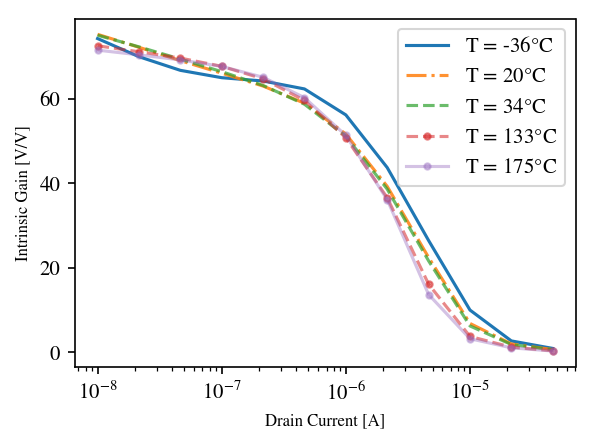
\includegraphics[width=\textwidth]{Av_nel_id}
		\resizebox {\textwidth} {!} {
			%% Creator: Matplotlib, PGF backend
%%
%% To include the figure in your LaTeX document, write
%%   \input{<filename>.pgf}
%%
%% Make sure the required packages are loaded in your preamble
%%   \usepackage{pgf}
%%
%% Figures using additional raster images can only be included by \input if
%% they are in the same directory as the main LaTeX file. For loading figures
%% from other directories you can use the `import` package
%%   \usepackage{import}
%% and then include the figures with
%%   \import{<path to file>}{<filename>.pgf}
%%
%% Matplotlib used the following preamble
%%   \usepackage{gensymb}
%%   \usepackage[utf8x]{inputenc}
%%   \usepackage[T1]{fontenc}
%%
\begingroup%
\makeatletter%
\begin{pgfpicture}%
\pgfpathrectangle{\pgfpointorigin}{\pgfqpoint{3.840000in}{2.840000in}}%
\pgfusepath{use as bounding box, clip}%
\begin{pgfscope}%
\pgfsetbuttcap%
\pgfsetmiterjoin%
\definecolor{currentfill}{rgb}{1.000000,1.000000,1.000000}%
\pgfsetfillcolor{currentfill}%
\pgfsetlinewidth{0.000000pt}%
\definecolor{currentstroke}{rgb}{1.000000,1.000000,1.000000}%
\pgfsetstrokecolor{currentstroke}%
\pgfsetdash{}{0pt}%
\pgfpathmoveto{\pgfqpoint{0.000000in}{0.000000in}}%
\pgfpathlineto{\pgfqpoint{3.840000in}{0.000000in}}%
\pgfpathlineto{\pgfqpoint{3.840000in}{2.840000in}}%
\pgfpathlineto{\pgfqpoint{0.000000in}{2.840000in}}%
\pgfpathclose%
\pgfusepath{fill}%
\end{pgfscope}%
\begin{pgfscope}%
\pgfsetbuttcap%
\pgfsetmiterjoin%
\definecolor{currentfill}{rgb}{1.000000,1.000000,1.000000}%
\pgfsetfillcolor{currentfill}%
\pgfsetlinewidth{0.000000pt}%
\definecolor{currentstroke}{rgb}{0.000000,0.000000,0.000000}%
\pgfsetstrokecolor{currentstroke}%
\pgfsetstrokeopacity{0.000000}%
\pgfsetdash{}{0pt}%
\pgfpathmoveto{\pgfqpoint{0.615235in}{0.596026in}}%
\pgfpathlineto{\pgfqpoint{3.716667in}{0.596026in}}%
\pgfpathlineto{\pgfqpoint{3.716667in}{2.716667in}}%
\pgfpathlineto{\pgfqpoint{0.615235in}{2.716667in}}%
\pgfpathclose%
\pgfusepath{fill}%
\end{pgfscope}%
\begin{pgfscope}%
\pgfsetbuttcap%
\pgfsetroundjoin%
\definecolor{currentfill}{rgb}{0.000000,0.000000,0.000000}%
\pgfsetfillcolor{currentfill}%
\pgfsetlinewidth{0.803000pt}%
\definecolor{currentstroke}{rgb}{0.000000,0.000000,0.000000}%
\pgfsetstrokecolor{currentstroke}%
\pgfsetdash{}{0pt}%
\pgfsys@defobject{currentmarker}{\pgfqpoint{0.000000in}{-0.048611in}}{\pgfqpoint{0.000000in}{0.000000in}}{%
\pgfpathmoveto{\pgfqpoint{0.000000in}{0.000000in}}%
\pgfpathlineto{\pgfqpoint{0.000000in}{-0.048611in}}%
\pgfusepath{stroke,fill}%
}%
\begin{pgfscope}%
\pgfsys@transformshift{0.756209in}{0.596026in}%
\pgfsys@useobject{currentmarker}{}%
\end{pgfscope}%
\end{pgfscope}%
\begin{pgfscope}%
\pgftext[x=0.756209in,y=0.498804in,,top]{\fontsize{14.000000}{16.800000}\selectfont \(\displaystyle 10^{-8}\)}%
\end{pgfscope}%
\begin{pgfscope}%
\pgfsetbuttcap%
\pgfsetroundjoin%
\definecolor{currentfill}{rgb}{0.000000,0.000000,0.000000}%
\pgfsetfillcolor{currentfill}%
\pgfsetlinewidth{0.803000pt}%
\definecolor{currentstroke}{rgb}{0.000000,0.000000,0.000000}%
\pgfsetstrokecolor{currentstroke}%
\pgfsetdash{}{0pt}%
\pgfsys@defobject{currentmarker}{\pgfqpoint{0.000000in}{-0.048611in}}{\pgfqpoint{0.000000in}{0.000000in}}{%
\pgfpathmoveto{\pgfqpoint{0.000000in}{0.000000in}}%
\pgfpathlineto{\pgfqpoint{0.000000in}{-0.048611in}}%
\pgfusepath{stroke,fill}%
}%
\begin{pgfscope}%
\pgfsys@transformshift{1.525151in}{0.596026in}%
\pgfsys@useobject{currentmarker}{}%
\end{pgfscope}%
\end{pgfscope}%
\begin{pgfscope}%
\pgftext[x=1.525151in,y=0.498804in,,top]{\fontsize{14.000000}{16.800000}\selectfont \(\displaystyle 10^{-7}\)}%
\end{pgfscope}%
\begin{pgfscope}%
\pgfsetbuttcap%
\pgfsetroundjoin%
\definecolor{currentfill}{rgb}{0.000000,0.000000,0.000000}%
\pgfsetfillcolor{currentfill}%
\pgfsetlinewidth{0.803000pt}%
\definecolor{currentstroke}{rgb}{0.000000,0.000000,0.000000}%
\pgfsetstrokecolor{currentstroke}%
\pgfsetdash{}{0pt}%
\pgfsys@defobject{currentmarker}{\pgfqpoint{0.000000in}{-0.048611in}}{\pgfqpoint{0.000000in}{0.000000in}}{%
\pgfpathmoveto{\pgfqpoint{0.000000in}{0.000000in}}%
\pgfpathlineto{\pgfqpoint{0.000000in}{-0.048611in}}%
\pgfusepath{stroke,fill}%
}%
\begin{pgfscope}%
\pgfsys@transformshift{2.294093in}{0.596026in}%
\pgfsys@useobject{currentmarker}{}%
\end{pgfscope}%
\end{pgfscope}%
\begin{pgfscope}%
\pgftext[x=2.294093in,y=0.498804in,,top]{\fontsize{14.000000}{16.800000}\selectfont \(\displaystyle 10^{-6}\)}%
\end{pgfscope}%
\begin{pgfscope}%
\pgfsetbuttcap%
\pgfsetroundjoin%
\definecolor{currentfill}{rgb}{0.000000,0.000000,0.000000}%
\pgfsetfillcolor{currentfill}%
\pgfsetlinewidth{0.803000pt}%
\definecolor{currentstroke}{rgb}{0.000000,0.000000,0.000000}%
\pgfsetstrokecolor{currentstroke}%
\pgfsetdash{}{0pt}%
\pgfsys@defobject{currentmarker}{\pgfqpoint{0.000000in}{-0.048611in}}{\pgfqpoint{0.000000in}{0.000000in}}{%
\pgfpathmoveto{\pgfqpoint{0.000000in}{0.000000in}}%
\pgfpathlineto{\pgfqpoint{0.000000in}{-0.048611in}}%
\pgfusepath{stroke,fill}%
}%
\begin{pgfscope}%
\pgfsys@transformshift{3.063035in}{0.596026in}%
\pgfsys@useobject{currentmarker}{}%
\end{pgfscope}%
\end{pgfscope}%
\begin{pgfscope}%
\pgftext[x=3.063035in,y=0.498804in,,top]{\fontsize{14.000000}{16.800000}\selectfont \(\displaystyle 10^{-5}\)}%
\end{pgfscope}%
\begin{pgfscope}%
\pgfsetbuttcap%
\pgfsetroundjoin%
\definecolor{currentfill}{rgb}{0.000000,0.000000,0.000000}%
\pgfsetfillcolor{currentfill}%
\pgfsetlinewidth{0.602250pt}%
\definecolor{currentstroke}{rgb}{0.000000,0.000000,0.000000}%
\pgfsetstrokecolor{currentstroke}%
\pgfsetdash{}{0pt}%
\pgfsys@defobject{currentmarker}{\pgfqpoint{0.000000in}{-0.027778in}}{\pgfqpoint{0.000000in}{0.000000in}}{%
\pgfpathmoveto{\pgfqpoint{0.000000in}{0.000000in}}%
\pgfpathlineto{\pgfqpoint{0.000000in}{-0.027778in}}%
\pgfusepath{stroke,fill}%
}%
\begin{pgfscope}%
\pgfsys@transformshift{0.637098in}{0.596026in}%
\pgfsys@useobject{currentmarker}{}%
\end{pgfscope}%
\end{pgfscope}%
\begin{pgfscope}%
\pgfsetbuttcap%
\pgfsetroundjoin%
\definecolor{currentfill}{rgb}{0.000000,0.000000,0.000000}%
\pgfsetfillcolor{currentfill}%
\pgfsetlinewidth{0.602250pt}%
\definecolor{currentstroke}{rgb}{0.000000,0.000000,0.000000}%
\pgfsetstrokecolor{currentstroke}%
\pgfsetdash{}{0pt}%
\pgfsys@defobject{currentmarker}{\pgfqpoint{0.000000in}{-0.027778in}}{\pgfqpoint{0.000000in}{0.000000in}}{%
\pgfpathmoveto{\pgfqpoint{0.000000in}{0.000000in}}%
\pgfpathlineto{\pgfqpoint{0.000000in}{-0.027778in}}%
\pgfusepath{stroke,fill}%
}%
\begin{pgfscope}%
\pgfsys@transformshift{0.681691in}{0.596026in}%
\pgfsys@useobject{currentmarker}{}%
\end{pgfscope}%
\end{pgfscope}%
\begin{pgfscope}%
\pgfsetbuttcap%
\pgfsetroundjoin%
\definecolor{currentfill}{rgb}{0.000000,0.000000,0.000000}%
\pgfsetfillcolor{currentfill}%
\pgfsetlinewidth{0.602250pt}%
\definecolor{currentstroke}{rgb}{0.000000,0.000000,0.000000}%
\pgfsetstrokecolor{currentstroke}%
\pgfsetdash{}{0pt}%
\pgfsys@defobject{currentmarker}{\pgfqpoint{0.000000in}{-0.027778in}}{\pgfqpoint{0.000000in}{0.000000in}}{%
\pgfpathmoveto{\pgfqpoint{0.000000in}{0.000000in}}%
\pgfpathlineto{\pgfqpoint{0.000000in}{-0.027778in}}%
\pgfusepath{stroke,fill}%
}%
\begin{pgfscope}%
\pgfsys@transformshift{0.721024in}{0.596026in}%
\pgfsys@useobject{currentmarker}{}%
\end{pgfscope}%
\end{pgfscope}%
\begin{pgfscope}%
\pgfsetbuttcap%
\pgfsetroundjoin%
\definecolor{currentfill}{rgb}{0.000000,0.000000,0.000000}%
\pgfsetfillcolor{currentfill}%
\pgfsetlinewidth{0.602250pt}%
\definecolor{currentstroke}{rgb}{0.000000,0.000000,0.000000}%
\pgfsetstrokecolor{currentstroke}%
\pgfsetdash{}{0pt}%
\pgfsys@defobject{currentmarker}{\pgfqpoint{0.000000in}{-0.027778in}}{\pgfqpoint{0.000000in}{0.000000in}}{%
\pgfpathmoveto{\pgfqpoint{0.000000in}{0.000000in}}%
\pgfpathlineto{\pgfqpoint{0.000000in}{-0.027778in}}%
\pgfusepath{stroke,fill}%
}%
\begin{pgfscope}%
\pgfsys@transformshift{0.987683in}{0.596026in}%
\pgfsys@useobject{currentmarker}{}%
\end{pgfscope}%
\end{pgfscope}%
\begin{pgfscope}%
\pgfsetbuttcap%
\pgfsetroundjoin%
\definecolor{currentfill}{rgb}{0.000000,0.000000,0.000000}%
\pgfsetfillcolor{currentfill}%
\pgfsetlinewidth{0.602250pt}%
\definecolor{currentstroke}{rgb}{0.000000,0.000000,0.000000}%
\pgfsetstrokecolor{currentstroke}%
\pgfsetdash{}{0pt}%
\pgfsys@defobject{currentmarker}{\pgfqpoint{0.000000in}{-0.027778in}}{\pgfqpoint{0.000000in}{0.000000in}}{%
\pgfpathmoveto{\pgfqpoint{0.000000in}{0.000000in}}%
\pgfpathlineto{\pgfqpoint{0.000000in}{-0.027778in}}%
\pgfusepath{stroke,fill}%
}%
\begin{pgfscope}%
\pgfsys@transformshift{1.123087in}{0.596026in}%
\pgfsys@useobject{currentmarker}{}%
\end{pgfscope}%
\end{pgfscope}%
\begin{pgfscope}%
\pgfsetbuttcap%
\pgfsetroundjoin%
\definecolor{currentfill}{rgb}{0.000000,0.000000,0.000000}%
\pgfsetfillcolor{currentfill}%
\pgfsetlinewidth{0.602250pt}%
\definecolor{currentstroke}{rgb}{0.000000,0.000000,0.000000}%
\pgfsetstrokecolor{currentstroke}%
\pgfsetdash{}{0pt}%
\pgfsys@defobject{currentmarker}{\pgfqpoint{0.000000in}{-0.027778in}}{\pgfqpoint{0.000000in}{0.000000in}}{%
\pgfpathmoveto{\pgfqpoint{0.000000in}{0.000000in}}%
\pgfpathlineto{\pgfqpoint{0.000000in}{-0.027778in}}%
\pgfusepath{stroke,fill}%
}%
\begin{pgfscope}%
\pgfsys@transformshift{1.219158in}{0.596026in}%
\pgfsys@useobject{currentmarker}{}%
\end{pgfscope}%
\end{pgfscope}%
\begin{pgfscope}%
\pgfsetbuttcap%
\pgfsetroundjoin%
\definecolor{currentfill}{rgb}{0.000000,0.000000,0.000000}%
\pgfsetfillcolor{currentfill}%
\pgfsetlinewidth{0.602250pt}%
\definecolor{currentstroke}{rgb}{0.000000,0.000000,0.000000}%
\pgfsetstrokecolor{currentstroke}%
\pgfsetdash{}{0pt}%
\pgfsys@defobject{currentmarker}{\pgfqpoint{0.000000in}{-0.027778in}}{\pgfqpoint{0.000000in}{0.000000in}}{%
\pgfpathmoveto{\pgfqpoint{0.000000in}{0.000000in}}%
\pgfpathlineto{\pgfqpoint{0.000000in}{-0.027778in}}%
\pgfusepath{stroke,fill}%
}%
\begin{pgfscope}%
\pgfsys@transformshift{1.293676in}{0.596026in}%
\pgfsys@useobject{currentmarker}{}%
\end{pgfscope}%
\end{pgfscope}%
\begin{pgfscope}%
\pgfsetbuttcap%
\pgfsetroundjoin%
\definecolor{currentfill}{rgb}{0.000000,0.000000,0.000000}%
\pgfsetfillcolor{currentfill}%
\pgfsetlinewidth{0.602250pt}%
\definecolor{currentstroke}{rgb}{0.000000,0.000000,0.000000}%
\pgfsetstrokecolor{currentstroke}%
\pgfsetdash{}{0pt}%
\pgfsys@defobject{currentmarker}{\pgfqpoint{0.000000in}{-0.027778in}}{\pgfqpoint{0.000000in}{0.000000in}}{%
\pgfpathmoveto{\pgfqpoint{0.000000in}{0.000000in}}%
\pgfpathlineto{\pgfqpoint{0.000000in}{-0.027778in}}%
\pgfusepath{stroke,fill}%
}%
\begin{pgfscope}%
\pgfsys@transformshift{1.354562in}{0.596026in}%
\pgfsys@useobject{currentmarker}{}%
\end{pgfscope}%
\end{pgfscope}%
\begin{pgfscope}%
\pgfsetbuttcap%
\pgfsetroundjoin%
\definecolor{currentfill}{rgb}{0.000000,0.000000,0.000000}%
\pgfsetfillcolor{currentfill}%
\pgfsetlinewidth{0.602250pt}%
\definecolor{currentstroke}{rgb}{0.000000,0.000000,0.000000}%
\pgfsetstrokecolor{currentstroke}%
\pgfsetdash{}{0pt}%
\pgfsys@defobject{currentmarker}{\pgfqpoint{0.000000in}{-0.027778in}}{\pgfqpoint{0.000000in}{0.000000in}}{%
\pgfpathmoveto{\pgfqpoint{0.000000in}{0.000000in}}%
\pgfpathlineto{\pgfqpoint{0.000000in}{-0.027778in}}%
\pgfusepath{stroke,fill}%
}%
\begin{pgfscope}%
\pgfsys@transformshift{1.406040in}{0.596026in}%
\pgfsys@useobject{currentmarker}{}%
\end{pgfscope}%
\end{pgfscope}%
\begin{pgfscope}%
\pgfsetbuttcap%
\pgfsetroundjoin%
\definecolor{currentfill}{rgb}{0.000000,0.000000,0.000000}%
\pgfsetfillcolor{currentfill}%
\pgfsetlinewidth{0.602250pt}%
\definecolor{currentstroke}{rgb}{0.000000,0.000000,0.000000}%
\pgfsetstrokecolor{currentstroke}%
\pgfsetdash{}{0pt}%
\pgfsys@defobject{currentmarker}{\pgfqpoint{0.000000in}{-0.027778in}}{\pgfqpoint{0.000000in}{0.000000in}}{%
\pgfpathmoveto{\pgfqpoint{0.000000in}{0.000000in}}%
\pgfpathlineto{\pgfqpoint{0.000000in}{-0.027778in}}%
\pgfusepath{stroke,fill}%
}%
\begin{pgfscope}%
\pgfsys@transformshift{1.450633in}{0.596026in}%
\pgfsys@useobject{currentmarker}{}%
\end{pgfscope}%
\end{pgfscope}%
\begin{pgfscope}%
\pgfsetbuttcap%
\pgfsetroundjoin%
\definecolor{currentfill}{rgb}{0.000000,0.000000,0.000000}%
\pgfsetfillcolor{currentfill}%
\pgfsetlinewidth{0.602250pt}%
\definecolor{currentstroke}{rgb}{0.000000,0.000000,0.000000}%
\pgfsetstrokecolor{currentstroke}%
\pgfsetdash{}{0pt}%
\pgfsys@defobject{currentmarker}{\pgfqpoint{0.000000in}{-0.027778in}}{\pgfqpoint{0.000000in}{0.000000in}}{%
\pgfpathmoveto{\pgfqpoint{0.000000in}{0.000000in}}%
\pgfpathlineto{\pgfqpoint{0.000000in}{-0.027778in}}%
\pgfusepath{stroke,fill}%
}%
\begin{pgfscope}%
\pgfsys@transformshift{1.489966in}{0.596026in}%
\pgfsys@useobject{currentmarker}{}%
\end{pgfscope}%
\end{pgfscope}%
\begin{pgfscope}%
\pgfsetbuttcap%
\pgfsetroundjoin%
\definecolor{currentfill}{rgb}{0.000000,0.000000,0.000000}%
\pgfsetfillcolor{currentfill}%
\pgfsetlinewidth{0.602250pt}%
\definecolor{currentstroke}{rgb}{0.000000,0.000000,0.000000}%
\pgfsetstrokecolor{currentstroke}%
\pgfsetdash{}{0pt}%
\pgfsys@defobject{currentmarker}{\pgfqpoint{0.000000in}{-0.027778in}}{\pgfqpoint{0.000000in}{0.000000in}}{%
\pgfpathmoveto{\pgfqpoint{0.000000in}{0.000000in}}%
\pgfpathlineto{\pgfqpoint{0.000000in}{-0.027778in}}%
\pgfusepath{stroke,fill}%
}%
\begin{pgfscope}%
\pgfsys@transformshift{1.756625in}{0.596026in}%
\pgfsys@useobject{currentmarker}{}%
\end{pgfscope}%
\end{pgfscope}%
\begin{pgfscope}%
\pgfsetbuttcap%
\pgfsetroundjoin%
\definecolor{currentfill}{rgb}{0.000000,0.000000,0.000000}%
\pgfsetfillcolor{currentfill}%
\pgfsetlinewidth{0.602250pt}%
\definecolor{currentstroke}{rgb}{0.000000,0.000000,0.000000}%
\pgfsetstrokecolor{currentstroke}%
\pgfsetdash{}{0pt}%
\pgfsys@defobject{currentmarker}{\pgfqpoint{0.000000in}{-0.027778in}}{\pgfqpoint{0.000000in}{0.000000in}}{%
\pgfpathmoveto{\pgfqpoint{0.000000in}{0.000000in}}%
\pgfpathlineto{\pgfqpoint{0.000000in}{-0.027778in}}%
\pgfusepath{stroke,fill}%
}%
\begin{pgfscope}%
\pgfsys@transformshift{1.892029in}{0.596026in}%
\pgfsys@useobject{currentmarker}{}%
\end{pgfscope}%
\end{pgfscope}%
\begin{pgfscope}%
\pgfsetbuttcap%
\pgfsetroundjoin%
\definecolor{currentfill}{rgb}{0.000000,0.000000,0.000000}%
\pgfsetfillcolor{currentfill}%
\pgfsetlinewidth{0.602250pt}%
\definecolor{currentstroke}{rgb}{0.000000,0.000000,0.000000}%
\pgfsetstrokecolor{currentstroke}%
\pgfsetdash{}{0pt}%
\pgfsys@defobject{currentmarker}{\pgfqpoint{0.000000in}{-0.027778in}}{\pgfqpoint{0.000000in}{0.000000in}}{%
\pgfpathmoveto{\pgfqpoint{0.000000in}{0.000000in}}%
\pgfpathlineto{\pgfqpoint{0.000000in}{-0.027778in}}%
\pgfusepath{stroke,fill}%
}%
\begin{pgfscope}%
\pgfsys@transformshift{1.988100in}{0.596026in}%
\pgfsys@useobject{currentmarker}{}%
\end{pgfscope}%
\end{pgfscope}%
\begin{pgfscope}%
\pgfsetbuttcap%
\pgfsetroundjoin%
\definecolor{currentfill}{rgb}{0.000000,0.000000,0.000000}%
\pgfsetfillcolor{currentfill}%
\pgfsetlinewidth{0.602250pt}%
\definecolor{currentstroke}{rgb}{0.000000,0.000000,0.000000}%
\pgfsetstrokecolor{currentstroke}%
\pgfsetdash{}{0pt}%
\pgfsys@defobject{currentmarker}{\pgfqpoint{0.000000in}{-0.027778in}}{\pgfqpoint{0.000000in}{0.000000in}}{%
\pgfpathmoveto{\pgfqpoint{0.000000in}{0.000000in}}%
\pgfpathlineto{\pgfqpoint{0.000000in}{-0.027778in}}%
\pgfusepath{stroke,fill}%
}%
\begin{pgfscope}%
\pgfsys@transformshift{2.062618in}{0.596026in}%
\pgfsys@useobject{currentmarker}{}%
\end{pgfscope}%
\end{pgfscope}%
\begin{pgfscope}%
\pgfsetbuttcap%
\pgfsetroundjoin%
\definecolor{currentfill}{rgb}{0.000000,0.000000,0.000000}%
\pgfsetfillcolor{currentfill}%
\pgfsetlinewidth{0.602250pt}%
\definecolor{currentstroke}{rgb}{0.000000,0.000000,0.000000}%
\pgfsetstrokecolor{currentstroke}%
\pgfsetdash{}{0pt}%
\pgfsys@defobject{currentmarker}{\pgfqpoint{0.000000in}{-0.027778in}}{\pgfqpoint{0.000000in}{0.000000in}}{%
\pgfpathmoveto{\pgfqpoint{0.000000in}{0.000000in}}%
\pgfpathlineto{\pgfqpoint{0.000000in}{-0.027778in}}%
\pgfusepath{stroke,fill}%
}%
\begin{pgfscope}%
\pgfsys@transformshift{2.123504in}{0.596026in}%
\pgfsys@useobject{currentmarker}{}%
\end{pgfscope}%
\end{pgfscope}%
\begin{pgfscope}%
\pgfsetbuttcap%
\pgfsetroundjoin%
\definecolor{currentfill}{rgb}{0.000000,0.000000,0.000000}%
\pgfsetfillcolor{currentfill}%
\pgfsetlinewidth{0.602250pt}%
\definecolor{currentstroke}{rgb}{0.000000,0.000000,0.000000}%
\pgfsetstrokecolor{currentstroke}%
\pgfsetdash{}{0pt}%
\pgfsys@defobject{currentmarker}{\pgfqpoint{0.000000in}{-0.027778in}}{\pgfqpoint{0.000000in}{0.000000in}}{%
\pgfpathmoveto{\pgfqpoint{0.000000in}{0.000000in}}%
\pgfpathlineto{\pgfqpoint{0.000000in}{-0.027778in}}%
\pgfusepath{stroke,fill}%
}%
\begin{pgfscope}%
\pgfsys@transformshift{2.174982in}{0.596026in}%
\pgfsys@useobject{currentmarker}{}%
\end{pgfscope}%
\end{pgfscope}%
\begin{pgfscope}%
\pgfsetbuttcap%
\pgfsetroundjoin%
\definecolor{currentfill}{rgb}{0.000000,0.000000,0.000000}%
\pgfsetfillcolor{currentfill}%
\pgfsetlinewidth{0.602250pt}%
\definecolor{currentstroke}{rgb}{0.000000,0.000000,0.000000}%
\pgfsetstrokecolor{currentstroke}%
\pgfsetdash{}{0pt}%
\pgfsys@defobject{currentmarker}{\pgfqpoint{0.000000in}{-0.027778in}}{\pgfqpoint{0.000000in}{0.000000in}}{%
\pgfpathmoveto{\pgfqpoint{0.000000in}{0.000000in}}%
\pgfpathlineto{\pgfqpoint{0.000000in}{-0.027778in}}%
\pgfusepath{stroke,fill}%
}%
\begin{pgfscope}%
\pgfsys@transformshift{2.219575in}{0.596026in}%
\pgfsys@useobject{currentmarker}{}%
\end{pgfscope}%
\end{pgfscope}%
\begin{pgfscope}%
\pgfsetbuttcap%
\pgfsetroundjoin%
\definecolor{currentfill}{rgb}{0.000000,0.000000,0.000000}%
\pgfsetfillcolor{currentfill}%
\pgfsetlinewidth{0.602250pt}%
\definecolor{currentstroke}{rgb}{0.000000,0.000000,0.000000}%
\pgfsetstrokecolor{currentstroke}%
\pgfsetdash{}{0pt}%
\pgfsys@defobject{currentmarker}{\pgfqpoint{0.000000in}{-0.027778in}}{\pgfqpoint{0.000000in}{0.000000in}}{%
\pgfpathmoveto{\pgfqpoint{0.000000in}{0.000000in}}%
\pgfpathlineto{\pgfqpoint{0.000000in}{-0.027778in}}%
\pgfusepath{stroke,fill}%
}%
\begin{pgfscope}%
\pgfsys@transformshift{2.258908in}{0.596026in}%
\pgfsys@useobject{currentmarker}{}%
\end{pgfscope}%
\end{pgfscope}%
\begin{pgfscope}%
\pgfsetbuttcap%
\pgfsetroundjoin%
\definecolor{currentfill}{rgb}{0.000000,0.000000,0.000000}%
\pgfsetfillcolor{currentfill}%
\pgfsetlinewidth{0.602250pt}%
\definecolor{currentstroke}{rgb}{0.000000,0.000000,0.000000}%
\pgfsetstrokecolor{currentstroke}%
\pgfsetdash{}{0pt}%
\pgfsys@defobject{currentmarker}{\pgfqpoint{0.000000in}{-0.027778in}}{\pgfqpoint{0.000000in}{0.000000in}}{%
\pgfpathmoveto{\pgfqpoint{0.000000in}{0.000000in}}%
\pgfpathlineto{\pgfqpoint{0.000000in}{-0.027778in}}%
\pgfusepath{stroke,fill}%
}%
\begin{pgfscope}%
\pgfsys@transformshift{2.525567in}{0.596026in}%
\pgfsys@useobject{currentmarker}{}%
\end{pgfscope}%
\end{pgfscope}%
\begin{pgfscope}%
\pgfsetbuttcap%
\pgfsetroundjoin%
\definecolor{currentfill}{rgb}{0.000000,0.000000,0.000000}%
\pgfsetfillcolor{currentfill}%
\pgfsetlinewidth{0.602250pt}%
\definecolor{currentstroke}{rgb}{0.000000,0.000000,0.000000}%
\pgfsetstrokecolor{currentstroke}%
\pgfsetdash{}{0pt}%
\pgfsys@defobject{currentmarker}{\pgfqpoint{0.000000in}{-0.027778in}}{\pgfqpoint{0.000000in}{0.000000in}}{%
\pgfpathmoveto{\pgfqpoint{0.000000in}{0.000000in}}%
\pgfpathlineto{\pgfqpoint{0.000000in}{-0.027778in}}%
\pgfusepath{stroke,fill}%
}%
\begin{pgfscope}%
\pgfsys@transformshift{2.660971in}{0.596026in}%
\pgfsys@useobject{currentmarker}{}%
\end{pgfscope}%
\end{pgfscope}%
\begin{pgfscope}%
\pgfsetbuttcap%
\pgfsetroundjoin%
\definecolor{currentfill}{rgb}{0.000000,0.000000,0.000000}%
\pgfsetfillcolor{currentfill}%
\pgfsetlinewidth{0.602250pt}%
\definecolor{currentstroke}{rgb}{0.000000,0.000000,0.000000}%
\pgfsetstrokecolor{currentstroke}%
\pgfsetdash{}{0pt}%
\pgfsys@defobject{currentmarker}{\pgfqpoint{0.000000in}{-0.027778in}}{\pgfqpoint{0.000000in}{0.000000in}}{%
\pgfpathmoveto{\pgfqpoint{0.000000in}{0.000000in}}%
\pgfpathlineto{\pgfqpoint{0.000000in}{-0.027778in}}%
\pgfusepath{stroke,fill}%
}%
\begin{pgfscope}%
\pgfsys@transformshift{2.757042in}{0.596026in}%
\pgfsys@useobject{currentmarker}{}%
\end{pgfscope}%
\end{pgfscope}%
\begin{pgfscope}%
\pgfsetbuttcap%
\pgfsetroundjoin%
\definecolor{currentfill}{rgb}{0.000000,0.000000,0.000000}%
\pgfsetfillcolor{currentfill}%
\pgfsetlinewidth{0.602250pt}%
\definecolor{currentstroke}{rgb}{0.000000,0.000000,0.000000}%
\pgfsetstrokecolor{currentstroke}%
\pgfsetdash{}{0pt}%
\pgfsys@defobject{currentmarker}{\pgfqpoint{0.000000in}{-0.027778in}}{\pgfqpoint{0.000000in}{0.000000in}}{%
\pgfpathmoveto{\pgfqpoint{0.000000in}{0.000000in}}%
\pgfpathlineto{\pgfqpoint{0.000000in}{-0.027778in}}%
\pgfusepath{stroke,fill}%
}%
\begin{pgfscope}%
\pgfsys@transformshift{2.831560in}{0.596026in}%
\pgfsys@useobject{currentmarker}{}%
\end{pgfscope}%
\end{pgfscope}%
\begin{pgfscope}%
\pgfsetbuttcap%
\pgfsetroundjoin%
\definecolor{currentfill}{rgb}{0.000000,0.000000,0.000000}%
\pgfsetfillcolor{currentfill}%
\pgfsetlinewidth{0.602250pt}%
\definecolor{currentstroke}{rgb}{0.000000,0.000000,0.000000}%
\pgfsetstrokecolor{currentstroke}%
\pgfsetdash{}{0pt}%
\pgfsys@defobject{currentmarker}{\pgfqpoint{0.000000in}{-0.027778in}}{\pgfqpoint{0.000000in}{0.000000in}}{%
\pgfpathmoveto{\pgfqpoint{0.000000in}{0.000000in}}%
\pgfpathlineto{\pgfqpoint{0.000000in}{-0.027778in}}%
\pgfusepath{stroke,fill}%
}%
\begin{pgfscope}%
\pgfsys@transformshift{2.892446in}{0.596026in}%
\pgfsys@useobject{currentmarker}{}%
\end{pgfscope}%
\end{pgfscope}%
\begin{pgfscope}%
\pgfsetbuttcap%
\pgfsetroundjoin%
\definecolor{currentfill}{rgb}{0.000000,0.000000,0.000000}%
\pgfsetfillcolor{currentfill}%
\pgfsetlinewidth{0.602250pt}%
\definecolor{currentstroke}{rgb}{0.000000,0.000000,0.000000}%
\pgfsetstrokecolor{currentstroke}%
\pgfsetdash{}{0pt}%
\pgfsys@defobject{currentmarker}{\pgfqpoint{0.000000in}{-0.027778in}}{\pgfqpoint{0.000000in}{0.000000in}}{%
\pgfpathmoveto{\pgfqpoint{0.000000in}{0.000000in}}%
\pgfpathlineto{\pgfqpoint{0.000000in}{-0.027778in}}%
\pgfusepath{stroke,fill}%
}%
\begin{pgfscope}%
\pgfsys@transformshift{2.943924in}{0.596026in}%
\pgfsys@useobject{currentmarker}{}%
\end{pgfscope}%
\end{pgfscope}%
\begin{pgfscope}%
\pgfsetbuttcap%
\pgfsetroundjoin%
\definecolor{currentfill}{rgb}{0.000000,0.000000,0.000000}%
\pgfsetfillcolor{currentfill}%
\pgfsetlinewidth{0.602250pt}%
\definecolor{currentstroke}{rgb}{0.000000,0.000000,0.000000}%
\pgfsetstrokecolor{currentstroke}%
\pgfsetdash{}{0pt}%
\pgfsys@defobject{currentmarker}{\pgfqpoint{0.000000in}{-0.027778in}}{\pgfqpoint{0.000000in}{0.000000in}}{%
\pgfpathmoveto{\pgfqpoint{0.000000in}{0.000000in}}%
\pgfpathlineto{\pgfqpoint{0.000000in}{-0.027778in}}%
\pgfusepath{stroke,fill}%
}%
\begin{pgfscope}%
\pgfsys@transformshift{2.988517in}{0.596026in}%
\pgfsys@useobject{currentmarker}{}%
\end{pgfscope}%
\end{pgfscope}%
\begin{pgfscope}%
\pgfsetbuttcap%
\pgfsetroundjoin%
\definecolor{currentfill}{rgb}{0.000000,0.000000,0.000000}%
\pgfsetfillcolor{currentfill}%
\pgfsetlinewidth{0.602250pt}%
\definecolor{currentstroke}{rgb}{0.000000,0.000000,0.000000}%
\pgfsetstrokecolor{currentstroke}%
\pgfsetdash{}{0pt}%
\pgfsys@defobject{currentmarker}{\pgfqpoint{0.000000in}{-0.027778in}}{\pgfqpoint{0.000000in}{0.000000in}}{%
\pgfpathmoveto{\pgfqpoint{0.000000in}{0.000000in}}%
\pgfpathlineto{\pgfqpoint{0.000000in}{-0.027778in}}%
\pgfusepath{stroke,fill}%
}%
\begin{pgfscope}%
\pgfsys@transformshift{3.027850in}{0.596026in}%
\pgfsys@useobject{currentmarker}{}%
\end{pgfscope}%
\end{pgfscope}%
\begin{pgfscope}%
\pgfsetbuttcap%
\pgfsetroundjoin%
\definecolor{currentfill}{rgb}{0.000000,0.000000,0.000000}%
\pgfsetfillcolor{currentfill}%
\pgfsetlinewidth{0.602250pt}%
\definecolor{currentstroke}{rgb}{0.000000,0.000000,0.000000}%
\pgfsetstrokecolor{currentstroke}%
\pgfsetdash{}{0pt}%
\pgfsys@defobject{currentmarker}{\pgfqpoint{0.000000in}{-0.027778in}}{\pgfqpoint{0.000000in}{0.000000in}}{%
\pgfpathmoveto{\pgfqpoint{0.000000in}{0.000000in}}%
\pgfpathlineto{\pgfqpoint{0.000000in}{-0.027778in}}%
\pgfusepath{stroke,fill}%
}%
\begin{pgfscope}%
\pgfsys@transformshift{3.294509in}{0.596026in}%
\pgfsys@useobject{currentmarker}{}%
\end{pgfscope}%
\end{pgfscope}%
\begin{pgfscope}%
\pgfsetbuttcap%
\pgfsetroundjoin%
\definecolor{currentfill}{rgb}{0.000000,0.000000,0.000000}%
\pgfsetfillcolor{currentfill}%
\pgfsetlinewidth{0.602250pt}%
\definecolor{currentstroke}{rgb}{0.000000,0.000000,0.000000}%
\pgfsetstrokecolor{currentstroke}%
\pgfsetdash{}{0pt}%
\pgfsys@defobject{currentmarker}{\pgfqpoint{0.000000in}{-0.027778in}}{\pgfqpoint{0.000000in}{0.000000in}}{%
\pgfpathmoveto{\pgfqpoint{0.000000in}{0.000000in}}%
\pgfpathlineto{\pgfqpoint{0.000000in}{-0.027778in}}%
\pgfusepath{stroke,fill}%
}%
\begin{pgfscope}%
\pgfsys@transformshift{3.429913in}{0.596026in}%
\pgfsys@useobject{currentmarker}{}%
\end{pgfscope}%
\end{pgfscope}%
\begin{pgfscope}%
\pgfsetbuttcap%
\pgfsetroundjoin%
\definecolor{currentfill}{rgb}{0.000000,0.000000,0.000000}%
\pgfsetfillcolor{currentfill}%
\pgfsetlinewidth{0.602250pt}%
\definecolor{currentstroke}{rgb}{0.000000,0.000000,0.000000}%
\pgfsetstrokecolor{currentstroke}%
\pgfsetdash{}{0pt}%
\pgfsys@defobject{currentmarker}{\pgfqpoint{0.000000in}{-0.027778in}}{\pgfqpoint{0.000000in}{0.000000in}}{%
\pgfpathmoveto{\pgfqpoint{0.000000in}{0.000000in}}%
\pgfpathlineto{\pgfqpoint{0.000000in}{-0.027778in}}%
\pgfusepath{stroke,fill}%
}%
\begin{pgfscope}%
\pgfsys@transformshift{3.525984in}{0.596026in}%
\pgfsys@useobject{currentmarker}{}%
\end{pgfscope}%
\end{pgfscope}%
\begin{pgfscope}%
\pgfsetbuttcap%
\pgfsetroundjoin%
\definecolor{currentfill}{rgb}{0.000000,0.000000,0.000000}%
\pgfsetfillcolor{currentfill}%
\pgfsetlinewidth{0.602250pt}%
\definecolor{currentstroke}{rgb}{0.000000,0.000000,0.000000}%
\pgfsetstrokecolor{currentstroke}%
\pgfsetdash{}{0pt}%
\pgfsys@defobject{currentmarker}{\pgfqpoint{0.000000in}{-0.027778in}}{\pgfqpoint{0.000000in}{0.000000in}}{%
\pgfpathmoveto{\pgfqpoint{0.000000in}{0.000000in}}%
\pgfpathlineto{\pgfqpoint{0.000000in}{-0.027778in}}%
\pgfusepath{stroke,fill}%
}%
\begin{pgfscope}%
\pgfsys@transformshift{3.600502in}{0.596026in}%
\pgfsys@useobject{currentmarker}{}%
\end{pgfscope}%
\end{pgfscope}%
\begin{pgfscope}%
\pgfsetbuttcap%
\pgfsetroundjoin%
\definecolor{currentfill}{rgb}{0.000000,0.000000,0.000000}%
\pgfsetfillcolor{currentfill}%
\pgfsetlinewidth{0.602250pt}%
\definecolor{currentstroke}{rgb}{0.000000,0.000000,0.000000}%
\pgfsetstrokecolor{currentstroke}%
\pgfsetdash{}{0pt}%
\pgfsys@defobject{currentmarker}{\pgfqpoint{0.000000in}{-0.027778in}}{\pgfqpoint{0.000000in}{0.000000in}}{%
\pgfpathmoveto{\pgfqpoint{0.000000in}{0.000000in}}%
\pgfpathlineto{\pgfqpoint{0.000000in}{-0.027778in}}%
\pgfusepath{stroke,fill}%
}%
\begin{pgfscope}%
\pgfsys@transformshift{3.661388in}{0.596026in}%
\pgfsys@useobject{currentmarker}{}%
\end{pgfscope}%
\end{pgfscope}%
\begin{pgfscope}%
\pgfsetbuttcap%
\pgfsetroundjoin%
\definecolor{currentfill}{rgb}{0.000000,0.000000,0.000000}%
\pgfsetfillcolor{currentfill}%
\pgfsetlinewidth{0.602250pt}%
\definecolor{currentstroke}{rgb}{0.000000,0.000000,0.000000}%
\pgfsetstrokecolor{currentstroke}%
\pgfsetdash{}{0pt}%
\pgfsys@defobject{currentmarker}{\pgfqpoint{0.000000in}{-0.027778in}}{\pgfqpoint{0.000000in}{0.000000in}}{%
\pgfpathmoveto{\pgfqpoint{0.000000in}{0.000000in}}%
\pgfpathlineto{\pgfqpoint{0.000000in}{-0.027778in}}%
\pgfusepath{stroke,fill}%
}%
\begin{pgfscope}%
\pgfsys@transformshift{3.712866in}{0.596026in}%
\pgfsys@useobject{currentmarker}{}%
\end{pgfscope}%
\end{pgfscope}%
\begin{pgfscope}%
\pgftext[x=2.165951in,y=0.266626in,,top]{\fontsize{12.000000}{14.400000}\selectfont Drain Current [A]}%
\end{pgfscope}%
\begin{pgfscope}%
\pgfsetbuttcap%
\pgfsetroundjoin%
\definecolor{currentfill}{rgb}{0.000000,0.000000,0.000000}%
\pgfsetfillcolor{currentfill}%
\pgfsetlinewidth{0.803000pt}%
\definecolor{currentstroke}{rgb}{0.000000,0.000000,0.000000}%
\pgfsetstrokecolor{currentstroke}%
\pgfsetdash{}{0pt}%
\pgfsys@defobject{currentmarker}{\pgfqpoint{-0.048611in}{0.000000in}}{\pgfqpoint{0.000000in}{0.000000in}}{%
\pgfpathmoveto{\pgfqpoint{0.000000in}{0.000000in}}%
\pgfpathlineto{\pgfqpoint{-0.048611in}{0.000000in}}%
\pgfusepath{stroke,fill}%
}%
\begin{pgfscope}%
\pgfsys@transformshift{0.615235in}{0.683579in}%
\pgfsys@useobject{currentmarker}{}%
\end{pgfscope}%
\end{pgfscope}%
\begin{pgfscope}%
\pgftext[x=0.420097in,y=0.614712in,left,base]{\fontsize{14.000000}{16.800000}\selectfont \(\displaystyle 0\)}%
\end{pgfscope}%
\begin{pgfscope}%
\pgfsetbuttcap%
\pgfsetroundjoin%
\definecolor{currentfill}{rgb}{0.000000,0.000000,0.000000}%
\pgfsetfillcolor{currentfill}%
\pgfsetlinewidth{0.803000pt}%
\definecolor{currentstroke}{rgb}{0.000000,0.000000,0.000000}%
\pgfsetstrokecolor{currentstroke}%
\pgfsetdash{}{0pt}%
\pgfsys@defobject{currentmarker}{\pgfqpoint{-0.048611in}{0.000000in}}{\pgfqpoint{0.000000in}{0.000000in}}{%
\pgfpathmoveto{\pgfqpoint{0.000000in}{0.000000in}}%
\pgfpathlineto{\pgfqpoint{-0.048611in}{0.000000in}}%
\pgfusepath{stroke,fill}%
}%
\begin{pgfscope}%
\pgfsys@transformshift{0.615235in}{1.198723in}%
\pgfsys@useobject{currentmarker}{}%
\end{pgfscope}%
\end{pgfscope}%
\begin{pgfscope}%
\pgftext[x=0.322182in,y=1.129857in,left,base]{\fontsize{14.000000}{16.800000}\selectfont \(\displaystyle 20\)}%
\end{pgfscope}%
\begin{pgfscope}%
\pgfsetbuttcap%
\pgfsetroundjoin%
\definecolor{currentfill}{rgb}{0.000000,0.000000,0.000000}%
\pgfsetfillcolor{currentfill}%
\pgfsetlinewidth{0.803000pt}%
\definecolor{currentstroke}{rgb}{0.000000,0.000000,0.000000}%
\pgfsetstrokecolor{currentstroke}%
\pgfsetdash{}{0pt}%
\pgfsys@defobject{currentmarker}{\pgfqpoint{-0.048611in}{0.000000in}}{\pgfqpoint{0.000000in}{0.000000in}}{%
\pgfpathmoveto{\pgfqpoint{0.000000in}{0.000000in}}%
\pgfpathlineto{\pgfqpoint{-0.048611in}{0.000000in}}%
\pgfusepath{stroke,fill}%
}%
\begin{pgfscope}%
\pgfsys@transformshift{0.615235in}{1.713868in}%
\pgfsys@useobject{currentmarker}{}%
\end{pgfscope}%
\end{pgfscope}%
\begin{pgfscope}%
\pgftext[x=0.322182in,y=1.645002in,left,base]{\fontsize{14.000000}{16.800000}\selectfont \(\displaystyle 40\)}%
\end{pgfscope}%
\begin{pgfscope}%
\pgfsetbuttcap%
\pgfsetroundjoin%
\definecolor{currentfill}{rgb}{0.000000,0.000000,0.000000}%
\pgfsetfillcolor{currentfill}%
\pgfsetlinewidth{0.803000pt}%
\definecolor{currentstroke}{rgb}{0.000000,0.000000,0.000000}%
\pgfsetstrokecolor{currentstroke}%
\pgfsetdash{}{0pt}%
\pgfsys@defobject{currentmarker}{\pgfqpoint{-0.048611in}{0.000000in}}{\pgfqpoint{0.000000in}{0.000000in}}{%
\pgfpathmoveto{\pgfqpoint{0.000000in}{0.000000in}}%
\pgfpathlineto{\pgfqpoint{-0.048611in}{0.000000in}}%
\pgfusepath{stroke,fill}%
}%
\begin{pgfscope}%
\pgfsys@transformshift{0.615235in}{2.229013in}%
\pgfsys@useobject{currentmarker}{}%
\end{pgfscope}%
\end{pgfscope}%
\begin{pgfscope}%
\pgftext[x=0.322182in,y=2.160147in,left,base]{\fontsize{14.000000}{16.800000}\selectfont \(\displaystyle 60\)}%
\end{pgfscope}%
\begin{pgfscope}%
\pgftext[x=0.266626in,y=1.656346in,,bottom,rotate=90.000000]{\fontsize{12.000000}{14.400000}\selectfont Intrinsic Gain [V/V]}%
\end{pgfscope}%
\begin{pgfscope}%
\pgfpathrectangle{\pgfqpoint{0.615235in}{0.596026in}}{\pgfqpoint{3.101432in}{2.120641in}} %
\pgfusepath{clip}%
\pgfsetrectcap%
\pgfsetroundjoin%
\pgfsetlinewidth{1.505625pt}%
\definecolor{currentstroke}{rgb}{0.121569,0.466667,0.705882}%
\pgfsetstrokecolor{currentstroke}%
\pgfsetdash{}{0pt}%
\pgfpathmoveto{\pgfqpoint{0.756209in}{2.594600in}}%
\pgfpathlineto{\pgfqpoint{1.012455in}{2.484137in}}%
\pgfpathlineto{\pgfqpoint{1.268866in}{2.401161in}}%
\pgfpathlineto{\pgfqpoint{1.525151in}{2.356314in}}%
\pgfpathlineto{\pgfqpoint{1.781397in}{2.336216in}}%
\pgfpathlineto{\pgfqpoint{2.037808in}{2.287875in}}%
\pgfpathlineto{\pgfqpoint{2.294093in}{2.129807in}}%
\pgfpathlineto{\pgfqpoint{2.550339in}{1.809131in}}%
\pgfpathlineto{\pgfqpoint{2.806750in}{1.365299in}}%
\pgfpathlineto{\pgfqpoint{3.063035in}{0.941906in}}%
\pgfpathlineto{\pgfqpoint{3.319282in}{0.753984in}}%
\pgfpathlineto{\pgfqpoint{3.575692in}{0.708329in}}%
\pgfusepath{stroke}%
\end{pgfscope}%
\begin{pgfscope}%
\pgfpathrectangle{\pgfqpoint{0.615235in}{0.596026in}}{\pgfqpoint{3.101432in}{2.120641in}} %
\pgfusepath{clip}%
\pgfsetbuttcap%
\pgfsetroundjoin%
\pgfsetlinewidth{1.505625pt}%
\definecolor{currentstroke}{rgb}{1.000000,0.498039,0.054902}%
\pgfsetstrokecolor{currentstroke}%
\pgfsetstrokeopacity{0.850000}%
\pgfsetdash{{9.600000pt}{2.400000pt}{1.500000pt}{2.400000pt}}{0.000000pt}%
\pgfpathmoveto{\pgfqpoint{0.756209in}{2.620274in}}%
\pgfpathlineto{\pgfqpoint{1.012455in}{2.541562in}}%
\pgfpathlineto{\pgfqpoint{1.268866in}{2.460299in}}%
\pgfpathlineto{\pgfqpoint{1.525151in}{2.383694in}}%
\pgfpathlineto{\pgfqpoint{1.781397in}{2.305436in}}%
\pgfpathlineto{\pgfqpoint{2.037808in}{2.201026in}}%
\pgfpathlineto{\pgfqpoint{2.294093in}{2.013267in}}%
\pgfpathlineto{\pgfqpoint{2.550339in}{1.694715in}}%
\pgfpathlineto{\pgfqpoint{2.806750in}{1.262059in}}%
\pgfpathlineto{\pgfqpoint{3.063035in}{0.860348in}}%
\pgfpathlineto{\pgfqpoint{3.319282in}{0.735453in}}%
\pgfpathlineto{\pgfqpoint{3.575692in}{0.701485in}}%
\pgfusepath{stroke}%
\end{pgfscope}%
\begin{pgfscope}%
\pgfpathrectangle{\pgfqpoint{0.615235in}{0.596026in}}{\pgfqpoint{3.101432in}{2.120641in}} %
\pgfusepath{clip}%
\pgfsetbuttcap%
\pgfsetroundjoin%
\pgfsetlinewidth{1.505625pt}%
\definecolor{currentstroke}{rgb}{0.172549,0.627451,0.172549}%
\pgfsetstrokecolor{currentstroke}%
\pgfsetstrokeopacity{0.700000}%
\pgfsetdash{{5.550000pt}{2.400000pt}}{0.000000pt}%
\pgfpathmoveto{\pgfqpoint{0.756209in}{2.614914in}}%
\pgfpathlineto{\pgfqpoint{1.012455in}{2.544138in}}%
\pgfpathlineto{\pgfqpoint{1.268866in}{2.469679in}}%
\pgfpathlineto{\pgfqpoint{1.525151in}{2.393024in}}%
\pgfpathlineto{\pgfqpoint{1.781397in}{2.309166in}}%
\pgfpathlineto{\pgfqpoint{2.037808in}{2.194893in}}%
\pgfpathlineto{\pgfqpoint{2.294093in}{1.999686in}}%
\pgfpathlineto{\pgfqpoint{2.550339in}{1.678137in}}%
\pgfpathlineto{\pgfqpoint{2.806750in}{1.241426in}}%
\pgfpathlineto{\pgfqpoint{3.063035in}{0.845141in}}%
\pgfpathlineto{\pgfqpoint{3.319282in}{0.732098in}}%
\pgfpathlineto{\pgfqpoint{3.575692in}{0.700206in}}%
\pgfusepath{stroke}%
\end{pgfscope}%
\begin{pgfscope}%
\pgfpathrectangle{\pgfqpoint{0.615235in}{0.596026in}}{\pgfqpoint{3.101432in}{2.120641in}} %
\pgfusepath{clip}%
\pgfsetbuttcap%
\pgfsetroundjoin%
\pgfsetlinewidth{1.505625pt}%
\definecolor{currentstroke}{rgb}{0.839216,0.152941,0.156863}%
\pgfsetstrokecolor{currentstroke}%
\pgfsetstrokeopacity{0.550000}%
\pgfsetdash{{5.550000pt}{2.400000pt}}{0.000000pt}%
\pgfpathmoveto{\pgfqpoint{0.756209in}{2.550488in}}%
\pgfpathlineto{\pgfqpoint{1.012455in}{2.514255in}}%
\pgfpathlineto{\pgfqpoint{1.268866in}{2.475782in}}%
\pgfpathlineto{\pgfqpoint{1.525151in}{2.425773in}}%
\pgfpathlineto{\pgfqpoint{1.781397in}{2.349634in}}%
\pgfpathlineto{\pgfqpoint{2.037808in}{2.218262in}}%
\pgfpathlineto{\pgfqpoint{2.294093in}{1.990850in}}%
\pgfpathlineto{\pgfqpoint{2.550339in}{1.625796in}}%
\pgfpathlineto{\pgfqpoint{2.806750in}{1.099341in}}%
\pgfpathlineto{\pgfqpoint{3.063035in}{0.781308in}}%
\pgfpathlineto{\pgfqpoint{3.319282in}{0.716165in}}%
\pgfpathlineto{\pgfqpoint{3.575692in}{0.694090in}}%
\pgfusepath{stroke}%
\end{pgfscope}%
\begin{pgfscope}%
\pgfpathrectangle{\pgfqpoint{0.615235in}{0.596026in}}{\pgfqpoint{3.101432in}{2.120641in}} %
\pgfusepath{clip}%
\pgfsetbuttcap%
\pgfsetroundjoin%
\definecolor{currentfill}{rgb}{0.839216,0.152941,0.156863}%
\pgfsetfillcolor{currentfill}%
\pgfsetfillopacity{0.550000}%
\pgfsetlinewidth{1.003750pt}%
\definecolor{currentstroke}{rgb}{0.839216,0.152941,0.156863}%
\pgfsetstrokecolor{currentstroke}%
\pgfsetstrokeopacity{0.550000}%
\pgfsetdash{}{0pt}%
\pgfsys@defobject{currentmarker}{\pgfqpoint{-0.020833in}{-0.020833in}}{\pgfqpoint{0.020833in}{0.020833in}}{%
\pgfpathmoveto{\pgfqpoint{0.000000in}{-0.020833in}}%
\pgfpathcurveto{\pgfqpoint{0.005525in}{-0.020833in}}{\pgfqpoint{0.010825in}{-0.018638in}}{\pgfqpoint{0.014731in}{-0.014731in}}%
\pgfpathcurveto{\pgfqpoint{0.018638in}{-0.010825in}}{\pgfqpoint{0.020833in}{-0.005525in}}{\pgfqpoint{0.020833in}{0.000000in}}%
\pgfpathcurveto{\pgfqpoint{0.020833in}{0.005525in}}{\pgfqpoint{0.018638in}{0.010825in}}{\pgfqpoint{0.014731in}{0.014731in}}%
\pgfpathcurveto{\pgfqpoint{0.010825in}{0.018638in}}{\pgfqpoint{0.005525in}{0.020833in}}{\pgfqpoint{0.000000in}{0.020833in}}%
\pgfpathcurveto{\pgfqpoint{-0.005525in}{0.020833in}}{\pgfqpoint{-0.010825in}{0.018638in}}{\pgfqpoint{-0.014731in}{0.014731in}}%
\pgfpathcurveto{\pgfqpoint{-0.018638in}{0.010825in}}{\pgfqpoint{-0.020833in}{0.005525in}}{\pgfqpoint{-0.020833in}{0.000000in}}%
\pgfpathcurveto{\pgfqpoint{-0.020833in}{-0.005525in}}{\pgfqpoint{-0.018638in}{-0.010825in}}{\pgfqpoint{-0.014731in}{-0.014731in}}%
\pgfpathcurveto{\pgfqpoint{-0.010825in}{-0.018638in}}{\pgfqpoint{-0.005525in}{-0.020833in}}{\pgfqpoint{0.000000in}{-0.020833in}}%
\pgfpathclose%
\pgfusepath{stroke,fill}%
}%
\begin{pgfscope}%
\pgfsys@transformshift{0.756209in}{2.550488in}%
\pgfsys@useobject{currentmarker}{}%
\end{pgfscope}%
\begin{pgfscope}%
\pgfsys@transformshift{1.012455in}{2.514255in}%
\pgfsys@useobject{currentmarker}{}%
\end{pgfscope}%
\begin{pgfscope}%
\pgfsys@transformshift{1.268866in}{2.475782in}%
\pgfsys@useobject{currentmarker}{}%
\end{pgfscope}%
\begin{pgfscope}%
\pgfsys@transformshift{1.525151in}{2.425773in}%
\pgfsys@useobject{currentmarker}{}%
\end{pgfscope}%
\begin{pgfscope}%
\pgfsys@transformshift{1.781397in}{2.349634in}%
\pgfsys@useobject{currentmarker}{}%
\end{pgfscope}%
\begin{pgfscope}%
\pgfsys@transformshift{2.037808in}{2.218262in}%
\pgfsys@useobject{currentmarker}{}%
\end{pgfscope}%
\begin{pgfscope}%
\pgfsys@transformshift{2.294093in}{1.990850in}%
\pgfsys@useobject{currentmarker}{}%
\end{pgfscope}%
\begin{pgfscope}%
\pgfsys@transformshift{2.550339in}{1.625796in}%
\pgfsys@useobject{currentmarker}{}%
\end{pgfscope}%
\begin{pgfscope}%
\pgfsys@transformshift{2.806750in}{1.099341in}%
\pgfsys@useobject{currentmarker}{}%
\end{pgfscope}%
\begin{pgfscope}%
\pgfsys@transformshift{3.063035in}{0.781308in}%
\pgfsys@useobject{currentmarker}{}%
\end{pgfscope}%
\begin{pgfscope}%
\pgfsys@transformshift{3.319282in}{0.716165in}%
\pgfsys@useobject{currentmarker}{}%
\end{pgfscope}%
\begin{pgfscope}%
\pgfsys@transformshift{3.575692in}{0.694090in}%
\pgfsys@useobject{currentmarker}{}%
\end{pgfscope}%
\end{pgfscope}%
\begin{pgfscope}%
\pgfpathrectangle{\pgfqpoint{0.615235in}{0.596026in}}{\pgfqpoint{3.101432in}{2.120641in}} %
\pgfusepath{clip}%
\pgfsetrectcap%
\pgfsetroundjoin%
\pgfsetlinewidth{1.505625pt}%
\definecolor{currentstroke}{rgb}{0.580392,0.403922,0.741176}%
\pgfsetstrokecolor{currentstroke}%
\pgfsetstrokeopacity{0.400000}%
\pgfsetdash{}{0pt}%
\pgfpathmoveto{\pgfqpoint{0.756209in}{2.524051in}}%
\pgfpathlineto{\pgfqpoint{1.012455in}{2.495308in}}%
\pgfpathlineto{\pgfqpoint{1.268866in}{2.464492in}}%
\pgfpathlineto{\pgfqpoint{1.525151in}{2.424949in}}%
\pgfpathlineto{\pgfqpoint{1.781397in}{2.359136in}}%
\pgfpathlineto{\pgfqpoint{2.037808in}{2.234908in}}%
\pgfpathlineto{\pgfqpoint{2.294093in}{2.004805in}}%
\pgfpathlineto{\pgfqpoint{2.550339in}{1.613584in}}%
\pgfpathlineto{\pgfqpoint{2.806750in}{1.036428in}}%
\pgfpathlineto{\pgfqpoint{3.063035in}{0.767317in}}%
\pgfpathlineto{\pgfqpoint{3.319282in}{0.711884in}}%
\pgfpathlineto{\pgfqpoint{3.575692in}{0.692419in}}%
\pgfusepath{stroke}%
\end{pgfscope}%
\begin{pgfscope}%
\pgfpathrectangle{\pgfqpoint{0.615235in}{0.596026in}}{\pgfqpoint{3.101432in}{2.120641in}} %
\pgfusepath{clip}%
\pgfsetbuttcap%
\pgfsetroundjoin%
\definecolor{currentfill}{rgb}{0.580392,0.403922,0.741176}%
\pgfsetfillcolor{currentfill}%
\pgfsetfillopacity{0.400000}%
\pgfsetlinewidth{1.003750pt}%
\definecolor{currentstroke}{rgb}{0.580392,0.403922,0.741176}%
\pgfsetstrokecolor{currentstroke}%
\pgfsetstrokeopacity{0.400000}%
\pgfsetdash{}{0pt}%
\pgfsys@defobject{currentmarker}{\pgfqpoint{-0.020833in}{-0.020833in}}{\pgfqpoint{0.020833in}{0.020833in}}{%
\pgfpathmoveto{\pgfqpoint{0.000000in}{-0.020833in}}%
\pgfpathcurveto{\pgfqpoint{0.005525in}{-0.020833in}}{\pgfqpoint{0.010825in}{-0.018638in}}{\pgfqpoint{0.014731in}{-0.014731in}}%
\pgfpathcurveto{\pgfqpoint{0.018638in}{-0.010825in}}{\pgfqpoint{0.020833in}{-0.005525in}}{\pgfqpoint{0.020833in}{0.000000in}}%
\pgfpathcurveto{\pgfqpoint{0.020833in}{0.005525in}}{\pgfqpoint{0.018638in}{0.010825in}}{\pgfqpoint{0.014731in}{0.014731in}}%
\pgfpathcurveto{\pgfqpoint{0.010825in}{0.018638in}}{\pgfqpoint{0.005525in}{0.020833in}}{\pgfqpoint{0.000000in}{0.020833in}}%
\pgfpathcurveto{\pgfqpoint{-0.005525in}{0.020833in}}{\pgfqpoint{-0.010825in}{0.018638in}}{\pgfqpoint{-0.014731in}{0.014731in}}%
\pgfpathcurveto{\pgfqpoint{-0.018638in}{0.010825in}}{\pgfqpoint{-0.020833in}{0.005525in}}{\pgfqpoint{-0.020833in}{0.000000in}}%
\pgfpathcurveto{\pgfqpoint{-0.020833in}{-0.005525in}}{\pgfqpoint{-0.018638in}{-0.010825in}}{\pgfqpoint{-0.014731in}{-0.014731in}}%
\pgfpathcurveto{\pgfqpoint{-0.010825in}{-0.018638in}}{\pgfqpoint{-0.005525in}{-0.020833in}}{\pgfqpoint{0.000000in}{-0.020833in}}%
\pgfpathclose%
\pgfusepath{stroke,fill}%
}%
\begin{pgfscope}%
\pgfsys@transformshift{0.756209in}{2.524051in}%
\pgfsys@useobject{currentmarker}{}%
\end{pgfscope}%
\begin{pgfscope}%
\pgfsys@transformshift{1.012455in}{2.495308in}%
\pgfsys@useobject{currentmarker}{}%
\end{pgfscope}%
\begin{pgfscope}%
\pgfsys@transformshift{1.268866in}{2.464492in}%
\pgfsys@useobject{currentmarker}{}%
\end{pgfscope}%
\begin{pgfscope}%
\pgfsys@transformshift{1.525151in}{2.424949in}%
\pgfsys@useobject{currentmarker}{}%
\end{pgfscope}%
\begin{pgfscope}%
\pgfsys@transformshift{1.781397in}{2.359136in}%
\pgfsys@useobject{currentmarker}{}%
\end{pgfscope}%
\begin{pgfscope}%
\pgfsys@transformshift{2.037808in}{2.234908in}%
\pgfsys@useobject{currentmarker}{}%
\end{pgfscope}%
\begin{pgfscope}%
\pgfsys@transformshift{2.294093in}{2.004805in}%
\pgfsys@useobject{currentmarker}{}%
\end{pgfscope}%
\begin{pgfscope}%
\pgfsys@transformshift{2.550339in}{1.613584in}%
\pgfsys@useobject{currentmarker}{}%
\end{pgfscope}%
\begin{pgfscope}%
\pgfsys@transformshift{2.806750in}{1.036428in}%
\pgfsys@useobject{currentmarker}{}%
\end{pgfscope}%
\begin{pgfscope}%
\pgfsys@transformshift{3.063035in}{0.767317in}%
\pgfsys@useobject{currentmarker}{}%
\end{pgfscope}%
\begin{pgfscope}%
\pgfsys@transformshift{3.319282in}{0.711884in}%
\pgfsys@useobject{currentmarker}{}%
\end{pgfscope}%
\begin{pgfscope}%
\pgfsys@transformshift{3.575692in}{0.692419in}%
\pgfsys@useobject{currentmarker}{}%
\end{pgfscope}%
\end{pgfscope}%
\begin{pgfscope}%
\pgfsetrectcap%
\pgfsetmiterjoin%
\pgfsetlinewidth{0.803000pt}%
\definecolor{currentstroke}{rgb}{0.000000,0.000000,0.000000}%
\pgfsetstrokecolor{currentstroke}%
\pgfsetdash{}{0pt}%
\pgfpathmoveto{\pgfqpoint{0.615235in}{0.596026in}}%
\pgfpathlineto{\pgfqpoint{0.615235in}{2.716667in}}%
\pgfusepath{stroke}%
\end{pgfscope}%
\begin{pgfscope}%
\pgfsetrectcap%
\pgfsetmiterjoin%
\pgfsetlinewidth{0.803000pt}%
\definecolor{currentstroke}{rgb}{0.000000,0.000000,0.000000}%
\pgfsetstrokecolor{currentstroke}%
\pgfsetdash{}{0pt}%
\pgfpathmoveto{\pgfqpoint{3.716667in}{0.596026in}}%
\pgfpathlineto{\pgfqpoint{3.716667in}{2.716667in}}%
\pgfusepath{stroke}%
\end{pgfscope}%
\begin{pgfscope}%
\pgfsetrectcap%
\pgfsetmiterjoin%
\pgfsetlinewidth{0.803000pt}%
\definecolor{currentstroke}{rgb}{0.000000,0.000000,0.000000}%
\pgfsetstrokecolor{currentstroke}%
\pgfsetdash{}{0pt}%
\pgfpathmoveto{\pgfqpoint{0.615235in}{0.596026in}}%
\pgfpathlineto{\pgfqpoint{3.716667in}{0.596026in}}%
\pgfusepath{stroke}%
\end{pgfscope}%
\begin{pgfscope}%
\pgfsetrectcap%
\pgfsetmiterjoin%
\pgfsetlinewidth{0.803000pt}%
\definecolor{currentstroke}{rgb}{0.000000,0.000000,0.000000}%
\pgfsetstrokecolor{currentstroke}%
\pgfsetdash{}{0pt}%
\pgfpathmoveto{\pgfqpoint{0.615235in}{2.716667in}}%
\pgfpathlineto{\pgfqpoint{3.716667in}{2.716667in}}%
\pgfusepath{stroke}%
\end{pgfscope}%
\begin{pgfscope}%
\pgfsetbuttcap%
\pgfsetmiterjoin%
\definecolor{currentfill}{rgb}{1.000000,1.000000,1.000000}%
\pgfsetfillcolor{currentfill}%
\pgfsetfillopacity{0.800000}%
\pgfsetlinewidth{1.003750pt}%
\definecolor{currentstroke}{rgb}{0.800000,0.800000,0.800000}%
\pgfsetstrokecolor{currentstroke}%
\pgfsetstrokeopacity{0.800000}%
\pgfsetdash{}{0pt}%
\pgfpathmoveto{\pgfqpoint{0.712457in}{0.665470in}}%
\pgfpathlineto{\pgfqpoint{1.830171in}{0.665470in}}%
\pgfpathquadraticcurveto{\pgfqpoint{1.857948in}{0.665470in}}{\pgfqpoint{1.857948in}{0.693248in}}%
\pgfpathlineto{\pgfqpoint{1.857948in}{1.647691in}}%
\pgfpathquadraticcurveto{\pgfqpoint{1.857948in}{1.675468in}}{\pgfqpoint{1.830171in}{1.675468in}}%
\pgfpathlineto{\pgfqpoint{0.712457in}{1.675468in}}%
\pgfpathquadraticcurveto{\pgfqpoint{0.684679in}{1.675468in}}{\pgfqpoint{0.684679in}{1.647691in}}%
\pgfpathlineto{\pgfqpoint{0.684679in}{0.693248in}}%
\pgfpathquadraticcurveto{\pgfqpoint{0.684679in}{0.665470in}}{\pgfqpoint{0.712457in}{0.665470in}}%
\pgfpathclose%
\pgfusepath{stroke,fill}%
\end{pgfscope}%
\begin{pgfscope}%
\pgfsetrectcap%
\pgfsetroundjoin%
\pgfsetlinewidth{1.505625pt}%
\definecolor{currentstroke}{rgb}{0.121569,0.466667,0.705882}%
\pgfsetstrokecolor{currentstroke}%
\pgfsetdash{}{0pt}%
\pgfpathmoveto{\pgfqpoint{0.740235in}{1.571302in}}%
\pgfpathlineto{\pgfqpoint{1.018012in}{1.571302in}}%
\pgfusepath{stroke}%
\end{pgfscope}%
\begin{pgfscope}%
\pgftext[x=1.129123in,y=1.522691in,left,base]{\fontsize{10.000000}{12.000000}\selectfont T = -36\(\displaystyle \degree\)C}%
\end{pgfscope}%
\begin{pgfscope}%
\pgfsetbuttcap%
\pgfsetroundjoin%
\pgfsetlinewidth{1.505625pt}%
\definecolor{currentstroke}{rgb}{1.000000,0.498039,0.054902}%
\pgfsetstrokecolor{currentstroke}%
\pgfsetstrokeopacity{0.850000}%
\pgfsetdash{{9.600000pt}{2.400000pt}{1.500000pt}{2.400000pt}}{0.000000pt}%
\pgfpathmoveto{\pgfqpoint{0.740235in}{1.377635in}}%
\pgfpathlineto{\pgfqpoint{1.018012in}{1.377635in}}%
\pgfusepath{stroke}%
\end{pgfscope}%
\begin{pgfscope}%
\pgftext[x=1.129123in,y=1.329024in,left,base]{\fontsize{10.000000}{12.000000}\selectfont T = 20\(\displaystyle \degree\)C}%
\end{pgfscope}%
\begin{pgfscope}%
\pgfsetbuttcap%
\pgfsetroundjoin%
\pgfsetlinewidth{1.505625pt}%
\definecolor{currentstroke}{rgb}{0.172549,0.627451,0.172549}%
\pgfsetstrokecolor{currentstroke}%
\pgfsetstrokeopacity{0.700000}%
\pgfsetdash{{5.550000pt}{2.400000pt}}{0.000000pt}%
\pgfpathmoveto{\pgfqpoint{0.740235in}{1.183969in}}%
\pgfpathlineto{\pgfqpoint{1.018012in}{1.183969in}}%
\pgfusepath{stroke}%
\end{pgfscope}%
\begin{pgfscope}%
\pgftext[x=1.129123in,y=1.135358in,left,base]{\fontsize{10.000000}{12.000000}\selectfont T = 34\(\displaystyle \degree\)C}%
\end{pgfscope}%
\begin{pgfscope}%
\pgfsetbuttcap%
\pgfsetroundjoin%
\pgfsetlinewidth{1.505625pt}%
\definecolor{currentstroke}{rgb}{0.839216,0.152941,0.156863}%
\pgfsetstrokecolor{currentstroke}%
\pgfsetstrokeopacity{0.550000}%
\pgfsetdash{{5.550000pt}{2.400000pt}}{0.000000pt}%
\pgfpathmoveto{\pgfqpoint{0.740235in}{0.990303in}}%
\pgfpathlineto{\pgfqpoint{1.018012in}{0.990303in}}%
\pgfusepath{stroke}%
\end{pgfscope}%
\begin{pgfscope}%
\pgfsetbuttcap%
\pgfsetroundjoin%
\definecolor{currentfill}{rgb}{0.839216,0.152941,0.156863}%
\pgfsetfillcolor{currentfill}%
\pgfsetfillopacity{0.550000}%
\pgfsetlinewidth{1.003750pt}%
\definecolor{currentstroke}{rgb}{0.839216,0.152941,0.156863}%
\pgfsetstrokecolor{currentstroke}%
\pgfsetstrokeopacity{0.550000}%
\pgfsetdash{}{0pt}%
\pgfsys@defobject{currentmarker}{\pgfqpoint{-0.020833in}{-0.020833in}}{\pgfqpoint{0.020833in}{0.020833in}}{%
\pgfpathmoveto{\pgfqpoint{0.000000in}{-0.020833in}}%
\pgfpathcurveto{\pgfqpoint{0.005525in}{-0.020833in}}{\pgfqpoint{0.010825in}{-0.018638in}}{\pgfqpoint{0.014731in}{-0.014731in}}%
\pgfpathcurveto{\pgfqpoint{0.018638in}{-0.010825in}}{\pgfqpoint{0.020833in}{-0.005525in}}{\pgfqpoint{0.020833in}{0.000000in}}%
\pgfpathcurveto{\pgfqpoint{0.020833in}{0.005525in}}{\pgfqpoint{0.018638in}{0.010825in}}{\pgfqpoint{0.014731in}{0.014731in}}%
\pgfpathcurveto{\pgfqpoint{0.010825in}{0.018638in}}{\pgfqpoint{0.005525in}{0.020833in}}{\pgfqpoint{0.000000in}{0.020833in}}%
\pgfpathcurveto{\pgfqpoint{-0.005525in}{0.020833in}}{\pgfqpoint{-0.010825in}{0.018638in}}{\pgfqpoint{-0.014731in}{0.014731in}}%
\pgfpathcurveto{\pgfqpoint{-0.018638in}{0.010825in}}{\pgfqpoint{-0.020833in}{0.005525in}}{\pgfqpoint{-0.020833in}{0.000000in}}%
\pgfpathcurveto{\pgfqpoint{-0.020833in}{-0.005525in}}{\pgfqpoint{-0.018638in}{-0.010825in}}{\pgfqpoint{-0.014731in}{-0.014731in}}%
\pgfpathcurveto{\pgfqpoint{-0.010825in}{-0.018638in}}{\pgfqpoint{-0.005525in}{-0.020833in}}{\pgfqpoint{0.000000in}{-0.020833in}}%
\pgfpathclose%
\pgfusepath{stroke,fill}%
}%
\begin{pgfscope}%
\pgfsys@transformshift{0.879123in}{0.990303in}%
\pgfsys@useobject{currentmarker}{}%
\end{pgfscope}%
\end{pgfscope}%
\begin{pgfscope}%
\pgftext[x=1.129123in,y=0.941692in,left,base]{\fontsize{10.000000}{12.000000}\selectfont T = 133\(\displaystyle \degree\)C}%
\end{pgfscope}%
\begin{pgfscope}%
\pgfsetrectcap%
\pgfsetroundjoin%
\pgfsetlinewidth{1.505625pt}%
\definecolor{currentstroke}{rgb}{0.580392,0.403922,0.741176}%
\pgfsetstrokecolor{currentstroke}%
\pgfsetstrokeopacity{0.400000}%
\pgfsetdash{}{0pt}%
\pgfpathmoveto{\pgfqpoint{0.740235in}{0.796637in}}%
\pgfpathlineto{\pgfqpoint{1.018012in}{0.796637in}}%
\pgfusepath{stroke}%
\end{pgfscope}%
\begin{pgfscope}%
\pgfsetbuttcap%
\pgfsetroundjoin%
\definecolor{currentfill}{rgb}{0.580392,0.403922,0.741176}%
\pgfsetfillcolor{currentfill}%
\pgfsetfillopacity{0.400000}%
\pgfsetlinewidth{1.003750pt}%
\definecolor{currentstroke}{rgb}{0.580392,0.403922,0.741176}%
\pgfsetstrokecolor{currentstroke}%
\pgfsetstrokeopacity{0.400000}%
\pgfsetdash{}{0pt}%
\pgfsys@defobject{currentmarker}{\pgfqpoint{-0.020833in}{-0.020833in}}{\pgfqpoint{0.020833in}{0.020833in}}{%
\pgfpathmoveto{\pgfqpoint{0.000000in}{-0.020833in}}%
\pgfpathcurveto{\pgfqpoint{0.005525in}{-0.020833in}}{\pgfqpoint{0.010825in}{-0.018638in}}{\pgfqpoint{0.014731in}{-0.014731in}}%
\pgfpathcurveto{\pgfqpoint{0.018638in}{-0.010825in}}{\pgfqpoint{0.020833in}{-0.005525in}}{\pgfqpoint{0.020833in}{0.000000in}}%
\pgfpathcurveto{\pgfqpoint{0.020833in}{0.005525in}}{\pgfqpoint{0.018638in}{0.010825in}}{\pgfqpoint{0.014731in}{0.014731in}}%
\pgfpathcurveto{\pgfqpoint{0.010825in}{0.018638in}}{\pgfqpoint{0.005525in}{0.020833in}}{\pgfqpoint{0.000000in}{0.020833in}}%
\pgfpathcurveto{\pgfqpoint{-0.005525in}{0.020833in}}{\pgfqpoint{-0.010825in}{0.018638in}}{\pgfqpoint{-0.014731in}{0.014731in}}%
\pgfpathcurveto{\pgfqpoint{-0.018638in}{0.010825in}}{\pgfqpoint{-0.020833in}{0.005525in}}{\pgfqpoint{-0.020833in}{0.000000in}}%
\pgfpathcurveto{\pgfqpoint{-0.020833in}{-0.005525in}}{\pgfqpoint{-0.018638in}{-0.010825in}}{\pgfqpoint{-0.014731in}{-0.014731in}}%
\pgfpathcurveto{\pgfqpoint{-0.010825in}{-0.018638in}}{\pgfqpoint{-0.005525in}{-0.020833in}}{\pgfqpoint{0.000000in}{-0.020833in}}%
\pgfpathclose%
\pgfusepath{stroke,fill}%
}%
\begin{pgfscope}%
\pgfsys@transformshift{0.879123in}{0.796637in}%
\pgfsys@useobject{currentmarker}{}%
\end{pgfscope}%
\end{pgfscope}%
\begin{pgfscope}%
\pgftext[x=1.129123in,y=0.748026in,left,base]{\fontsize{10.000000}{12.000000}\selectfont T = 175\(\displaystyle \degree\)C}%
\end{pgfscope}%
\end{pgfpicture}%
\makeatother%
\endgroup%

		}
		\subcaption{Gain for L = 180 nm}
	\end{subfigure}
	\begin{subfigure}[b]{0.48\textwidth}
		%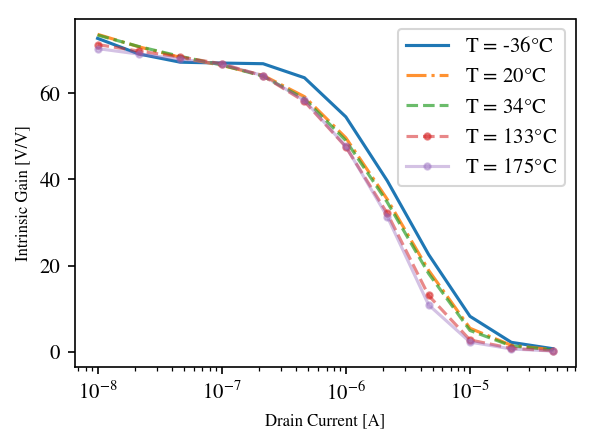
\includegraphics[width=\textwidth]{Av_nel_id_720}
		\resizebox {\textwidth} {!} {
			%% Creator: Matplotlib, PGF backend
%%
%% To include the figure in your LaTeX document, write
%%   \input{<filename>.pgf}
%%
%% Make sure the required packages are loaded in your preamble
%%   \usepackage{pgf}
%%
%% Figures using additional raster images can only be included by \input if
%% they are in the same directory as the main LaTeX file. For loading figures
%% from other directories you can use the `import` package
%%   \usepackage{import}
%% and then include the figures with
%%   \import{<path to file>}{<filename>.pgf}
%%
%% Matplotlib used the following preamble
%%   \usepackage{gensymb}
%%   \usepackage[utf8x]{inputenc}
%%   \usepackage[T1]{fontenc}
%%
\begingroup%
\makeatletter%
\begin{pgfpicture}%
\pgfpathrectangle{\pgfpointorigin}{\pgfqpoint{3.840000in}{2.840000in}}%
\pgfusepath{use as bounding box, clip}%
\begin{pgfscope}%
\pgfsetbuttcap%
\pgfsetmiterjoin%
\definecolor{currentfill}{rgb}{1.000000,1.000000,1.000000}%
\pgfsetfillcolor{currentfill}%
\pgfsetlinewidth{0.000000pt}%
\definecolor{currentstroke}{rgb}{1.000000,1.000000,1.000000}%
\pgfsetstrokecolor{currentstroke}%
\pgfsetdash{}{0pt}%
\pgfpathmoveto{\pgfqpoint{0.000000in}{0.000000in}}%
\pgfpathlineto{\pgfqpoint{3.840000in}{0.000000in}}%
\pgfpathlineto{\pgfqpoint{3.840000in}{2.840000in}}%
\pgfpathlineto{\pgfqpoint{0.000000in}{2.840000in}}%
\pgfpathclose%
\pgfusepath{fill}%
\end{pgfscope}%
\begin{pgfscope}%
\pgfsetbuttcap%
\pgfsetmiterjoin%
\definecolor{currentfill}{rgb}{1.000000,1.000000,1.000000}%
\pgfsetfillcolor{currentfill}%
\pgfsetlinewidth{0.000000pt}%
\definecolor{currentstroke}{rgb}{0.000000,0.000000,0.000000}%
\pgfsetstrokecolor{currentstroke}%
\pgfsetstrokeopacity{0.000000}%
\pgfsetdash{}{0pt}%
\pgfpathmoveto{\pgfqpoint{0.615235in}{0.596026in}}%
\pgfpathlineto{\pgfqpoint{3.716667in}{0.596026in}}%
\pgfpathlineto{\pgfqpoint{3.716667in}{2.716667in}}%
\pgfpathlineto{\pgfqpoint{0.615235in}{2.716667in}}%
\pgfpathclose%
\pgfusepath{fill}%
\end{pgfscope}%
\begin{pgfscope}%
\pgfsetbuttcap%
\pgfsetroundjoin%
\definecolor{currentfill}{rgb}{0.000000,0.000000,0.000000}%
\pgfsetfillcolor{currentfill}%
\pgfsetlinewidth{0.803000pt}%
\definecolor{currentstroke}{rgb}{0.000000,0.000000,0.000000}%
\pgfsetstrokecolor{currentstroke}%
\pgfsetdash{}{0pt}%
\pgfsys@defobject{currentmarker}{\pgfqpoint{0.000000in}{-0.048611in}}{\pgfqpoint{0.000000in}{0.000000in}}{%
\pgfpathmoveto{\pgfqpoint{0.000000in}{0.000000in}}%
\pgfpathlineto{\pgfqpoint{0.000000in}{-0.048611in}}%
\pgfusepath{stroke,fill}%
}%
\begin{pgfscope}%
\pgfsys@transformshift{0.756209in}{0.596026in}%
\pgfsys@useobject{currentmarker}{}%
\end{pgfscope}%
\end{pgfscope}%
\begin{pgfscope}%
\pgftext[x=0.756209in,y=0.498804in,,top]{\fontsize{14.000000}{16.800000}\selectfont \(\displaystyle 10^{-8}\)}%
\end{pgfscope}%
\begin{pgfscope}%
\pgfsetbuttcap%
\pgfsetroundjoin%
\definecolor{currentfill}{rgb}{0.000000,0.000000,0.000000}%
\pgfsetfillcolor{currentfill}%
\pgfsetlinewidth{0.803000pt}%
\definecolor{currentstroke}{rgb}{0.000000,0.000000,0.000000}%
\pgfsetstrokecolor{currentstroke}%
\pgfsetdash{}{0pt}%
\pgfsys@defobject{currentmarker}{\pgfqpoint{0.000000in}{-0.048611in}}{\pgfqpoint{0.000000in}{0.000000in}}{%
\pgfpathmoveto{\pgfqpoint{0.000000in}{0.000000in}}%
\pgfpathlineto{\pgfqpoint{0.000000in}{-0.048611in}}%
\pgfusepath{stroke,fill}%
}%
\begin{pgfscope}%
\pgfsys@transformshift{1.525151in}{0.596026in}%
\pgfsys@useobject{currentmarker}{}%
\end{pgfscope}%
\end{pgfscope}%
\begin{pgfscope}%
\pgftext[x=1.525151in,y=0.498804in,,top]{\fontsize{14.000000}{16.800000}\selectfont \(\displaystyle 10^{-7}\)}%
\end{pgfscope}%
\begin{pgfscope}%
\pgfsetbuttcap%
\pgfsetroundjoin%
\definecolor{currentfill}{rgb}{0.000000,0.000000,0.000000}%
\pgfsetfillcolor{currentfill}%
\pgfsetlinewidth{0.803000pt}%
\definecolor{currentstroke}{rgb}{0.000000,0.000000,0.000000}%
\pgfsetstrokecolor{currentstroke}%
\pgfsetdash{}{0pt}%
\pgfsys@defobject{currentmarker}{\pgfqpoint{0.000000in}{-0.048611in}}{\pgfqpoint{0.000000in}{0.000000in}}{%
\pgfpathmoveto{\pgfqpoint{0.000000in}{0.000000in}}%
\pgfpathlineto{\pgfqpoint{0.000000in}{-0.048611in}}%
\pgfusepath{stroke,fill}%
}%
\begin{pgfscope}%
\pgfsys@transformshift{2.294093in}{0.596026in}%
\pgfsys@useobject{currentmarker}{}%
\end{pgfscope}%
\end{pgfscope}%
\begin{pgfscope}%
\pgftext[x=2.294093in,y=0.498804in,,top]{\fontsize{14.000000}{16.800000}\selectfont \(\displaystyle 10^{-6}\)}%
\end{pgfscope}%
\begin{pgfscope}%
\pgfsetbuttcap%
\pgfsetroundjoin%
\definecolor{currentfill}{rgb}{0.000000,0.000000,0.000000}%
\pgfsetfillcolor{currentfill}%
\pgfsetlinewidth{0.803000pt}%
\definecolor{currentstroke}{rgb}{0.000000,0.000000,0.000000}%
\pgfsetstrokecolor{currentstroke}%
\pgfsetdash{}{0pt}%
\pgfsys@defobject{currentmarker}{\pgfqpoint{0.000000in}{-0.048611in}}{\pgfqpoint{0.000000in}{0.000000in}}{%
\pgfpathmoveto{\pgfqpoint{0.000000in}{0.000000in}}%
\pgfpathlineto{\pgfqpoint{0.000000in}{-0.048611in}}%
\pgfusepath{stroke,fill}%
}%
\begin{pgfscope}%
\pgfsys@transformshift{3.063035in}{0.596026in}%
\pgfsys@useobject{currentmarker}{}%
\end{pgfscope}%
\end{pgfscope}%
\begin{pgfscope}%
\pgftext[x=3.063035in,y=0.498804in,,top]{\fontsize{14.000000}{16.800000}\selectfont \(\displaystyle 10^{-5}\)}%
\end{pgfscope}%
\begin{pgfscope}%
\pgfsetbuttcap%
\pgfsetroundjoin%
\definecolor{currentfill}{rgb}{0.000000,0.000000,0.000000}%
\pgfsetfillcolor{currentfill}%
\pgfsetlinewidth{0.602250pt}%
\definecolor{currentstroke}{rgb}{0.000000,0.000000,0.000000}%
\pgfsetstrokecolor{currentstroke}%
\pgfsetdash{}{0pt}%
\pgfsys@defobject{currentmarker}{\pgfqpoint{0.000000in}{-0.027778in}}{\pgfqpoint{0.000000in}{0.000000in}}{%
\pgfpathmoveto{\pgfqpoint{0.000000in}{0.000000in}}%
\pgfpathlineto{\pgfqpoint{0.000000in}{-0.027778in}}%
\pgfusepath{stroke,fill}%
}%
\begin{pgfscope}%
\pgfsys@transformshift{0.637098in}{0.596026in}%
\pgfsys@useobject{currentmarker}{}%
\end{pgfscope}%
\end{pgfscope}%
\begin{pgfscope}%
\pgfsetbuttcap%
\pgfsetroundjoin%
\definecolor{currentfill}{rgb}{0.000000,0.000000,0.000000}%
\pgfsetfillcolor{currentfill}%
\pgfsetlinewidth{0.602250pt}%
\definecolor{currentstroke}{rgb}{0.000000,0.000000,0.000000}%
\pgfsetstrokecolor{currentstroke}%
\pgfsetdash{}{0pt}%
\pgfsys@defobject{currentmarker}{\pgfqpoint{0.000000in}{-0.027778in}}{\pgfqpoint{0.000000in}{0.000000in}}{%
\pgfpathmoveto{\pgfqpoint{0.000000in}{0.000000in}}%
\pgfpathlineto{\pgfqpoint{0.000000in}{-0.027778in}}%
\pgfusepath{stroke,fill}%
}%
\begin{pgfscope}%
\pgfsys@transformshift{0.681691in}{0.596026in}%
\pgfsys@useobject{currentmarker}{}%
\end{pgfscope}%
\end{pgfscope}%
\begin{pgfscope}%
\pgfsetbuttcap%
\pgfsetroundjoin%
\definecolor{currentfill}{rgb}{0.000000,0.000000,0.000000}%
\pgfsetfillcolor{currentfill}%
\pgfsetlinewidth{0.602250pt}%
\definecolor{currentstroke}{rgb}{0.000000,0.000000,0.000000}%
\pgfsetstrokecolor{currentstroke}%
\pgfsetdash{}{0pt}%
\pgfsys@defobject{currentmarker}{\pgfqpoint{0.000000in}{-0.027778in}}{\pgfqpoint{0.000000in}{0.000000in}}{%
\pgfpathmoveto{\pgfqpoint{0.000000in}{0.000000in}}%
\pgfpathlineto{\pgfqpoint{0.000000in}{-0.027778in}}%
\pgfusepath{stroke,fill}%
}%
\begin{pgfscope}%
\pgfsys@transformshift{0.721024in}{0.596026in}%
\pgfsys@useobject{currentmarker}{}%
\end{pgfscope}%
\end{pgfscope}%
\begin{pgfscope}%
\pgfsetbuttcap%
\pgfsetroundjoin%
\definecolor{currentfill}{rgb}{0.000000,0.000000,0.000000}%
\pgfsetfillcolor{currentfill}%
\pgfsetlinewidth{0.602250pt}%
\definecolor{currentstroke}{rgb}{0.000000,0.000000,0.000000}%
\pgfsetstrokecolor{currentstroke}%
\pgfsetdash{}{0pt}%
\pgfsys@defobject{currentmarker}{\pgfqpoint{0.000000in}{-0.027778in}}{\pgfqpoint{0.000000in}{0.000000in}}{%
\pgfpathmoveto{\pgfqpoint{0.000000in}{0.000000in}}%
\pgfpathlineto{\pgfqpoint{0.000000in}{-0.027778in}}%
\pgfusepath{stroke,fill}%
}%
\begin{pgfscope}%
\pgfsys@transformshift{0.987683in}{0.596026in}%
\pgfsys@useobject{currentmarker}{}%
\end{pgfscope}%
\end{pgfscope}%
\begin{pgfscope}%
\pgfsetbuttcap%
\pgfsetroundjoin%
\definecolor{currentfill}{rgb}{0.000000,0.000000,0.000000}%
\pgfsetfillcolor{currentfill}%
\pgfsetlinewidth{0.602250pt}%
\definecolor{currentstroke}{rgb}{0.000000,0.000000,0.000000}%
\pgfsetstrokecolor{currentstroke}%
\pgfsetdash{}{0pt}%
\pgfsys@defobject{currentmarker}{\pgfqpoint{0.000000in}{-0.027778in}}{\pgfqpoint{0.000000in}{0.000000in}}{%
\pgfpathmoveto{\pgfqpoint{0.000000in}{0.000000in}}%
\pgfpathlineto{\pgfqpoint{0.000000in}{-0.027778in}}%
\pgfusepath{stroke,fill}%
}%
\begin{pgfscope}%
\pgfsys@transformshift{1.123087in}{0.596026in}%
\pgfsys@useobject{currentmarker}{}%
\end{pgfscope}%
\end{pgfscope}%
\begin{pgfscope}%
\pgfsetbuttcap%
\pgfsetroundjoin%
\definecolor{currentfill}{rgb}{0.000000,0.000000,0.000000}%
\pgfsetfillcolor{currentfill}%
\pgfsetlinewidth{0.602250pt}%
\definecolor{currentstroke}{rgb}{0.000000,0.000000,0.000000}%
\pgfsetstrokecolor{currentstroke}%
\pgfsetdash{}{0pt}%
\pgfsys@defobject{currentmarker}{\pgfqpoint{0.000000in}{-0.027778in}}{\pgfqpoint{0.000000in}{0.000000in}}{%
\pgfpathmoveto{\pgfqpoint{0.000000in}{0.000000in}}%
\pgfpathlineto{\pgfqpoint{0.000000in}{-0.027778in}}%
\pgfusepath{stroke,fill}%
}%
\begin{pgfscope}%
\pgfsys@transformshift{1.219158in}{0.596026in}%
\pgfsys@useobject{currentmarker}{}%
\end{pgfscope}%
\end{pgfscope}%
\begin{pgfscope}%
\pgfsetbuttcap%
\pgfsetroundjoin%
\definecolor{currentfill}{rgb}{0.000000,0.000000,0.000000}%
\pgfsetfillcolor{currentfill}%
\pgfsetlinewidth{0.602250pt}%
\definecolor{currentstroke}{rgb}{0.000000,0.000000,0.000000}%
\pgfsetstrokecolor{currentstroke}%
\pgfsetdash{}{0pt}%
\pgfsys@defobject{currentmarker}{\pgfqpoint{0.000000in}{-0.027778in}}{\pgfqpoint{0.000000in}{0.000000in}}{%
\pgfpathmoveto{\pgfqpoint{0.000000in}{0.000000in}}%
\pgfpathlineto{\pgfqpoint{0.000000in}{-0.027778in}}%
\pgfusepath{stroke,fill}%
}%
\begin{pgfscope}%
\pgfsys@transformshift{1.293676in}{0.596026in}%
\pgfsys@useobject{currentmarker}{}%
\end{pgfscope}%
\end{pgfscope}%
\begin{pgfscope}%
\pgfsetbuttcap%
\pgfsetroundjoin%
\definecolor{currentfill}{rgb}{0.000000,0.000000,0.000000}%
\pgfsetfillcolor{currentfill}%
\pgfsetlinewidth{0.602250pt}%
\definecolor{currentstroke}{rgb}{0.000000,0.000000,0.000000}%
\pgfsetstrokecolor{currentstroke}%
\pgfsetdash{}{0pt}%
\pgfsys@defobject{currentmarker}{\pgfqpoint{0.000000in}{-0.027778in}}{\pgfqpoint{0.000000in}{0.000000in}}{%
\pgfpathmoveto{\pgfqpoint{0.000000in}{0.000000in}}%
\pgfpathlineto{\pgfqpoint{0.000000in}{-0.027778in}}%
\pgfusepath{stroke,fill}%
}%
\begin{pgfscope}%
\pgfsys@transformshift{1.354562in}{0.596026in}%
\pgfsys@useobject{currentmarker}{}%
\end{pgfscope}%
\end{pgfscope}%
\begin{pgfscope}%
\pgfsetbuttcap%
\pgfsetroundjoin%
\definecolor{currentfill}{rgb}{0.000000,0.000000,0.000000}%
\pgfsetfillcolor{currentfill}%
\pgfsetlinewidth{0.602250pt}%
\definecolor{currentstroke}{rgb}{0.000000,0.000000,0.000000}%
\pgfsetstrokecolor{currentstroke}%
\pgfsetdash{}{0pt}%
\pgfsys@defobject{currentmarker}{\pgfqpoint{0.000000in}{-0.027778in}}{\pgfqpoint{0.000000in}{0.000000in}}{%
\pgfpathmoveto{\pgfqpoint{0.000000in}{0.000000in}}%
\pgfpathlineto{\pgfqpoint{0.000000in}{-0.027778in}}%
\pgfusepath{stroke,fill}%
}%
\begin{pgfscope}%
\pgfsys@transformshift{1.406040in}{0.596026in}%
\pgfsys@useobject{currentmarker}{}%
\end{pgfscope}%
\end{pgfscope}%
\begin{pgfscope}%
\pgfsetbuttcap%
\pgfsetroundjoin%
\definecolor{currentfill}{rgb}{0.000000,0.000000,0.000000}%
\pgfsetfillcolor{currentfill}%
\pgfsetlinewidth{0.602250pt}%
\definecolor{currentstroke}{rgb}{0.000000,0.000000,0.000000}%
\pgfsetstrokecolor{currentstroke}%
\pgfsetdash{}{0pt}%
\pgfsys@defobject{currentmarker}{\pgfqpoint{0.000000in}{-0.027778in}}{\pgfqpoint{0.000000in}{0.000000in}}{%
\pgfpathmoveto{\pgfqpoint{0.000000in}{0.000000in}}%
\pgfpathlineto{\pgfqpoint{0.000000in}{-0.027778in}}%
\pgfusepath{stroke,fill}%
}%
\begin{pgfscope}%
\pgfsys@transformshift{1.450633in}{0.596026in}%
\pgfsys@useobject{currentmarker}{}%
\end{pgfscope}%
\end{pgfscope}%
\begin{pgfscope}%
\pgfsetbuttcap%
\pgfsetroundjoin%
\definecolor{currentfill}{rgb}{0.000000,0.000000,0.000000}%
\pgfsetfillcolor{currentfill}%
\pgfsetlinewidth{0.602250pt}%
\definecolor{currentstroke}{rgb}{0.000000,0.000000,0.000000}%
\pgfsetstrokecolor{currentstroke}%
\pgfsetdash{}{0pt}%
\pgfsys@defobject{currentmarker}{\pgfqpoint{0.000000in}{-0.027778in}}{\pgfqpoint{0.000000in}{0.000000in}}{%
\pgfpathmoveto{\pgfqpoint{0.000000in}{0.000000in}}%
\pgfpathlineto{\pgfqpoint{0.000000in}{-0.027778in}}%
\pgfusepath{stroke,fill}%
}%
\begin{pgfscope}%
\pgfsys@transformshift{1.489966in}{0.596026in}%
\pgfsys@useobject{currentmarker}{}%
\end{pgfscope}%
\end{pgfscope}%
\begin{pgfscope}%
\pgfsetbuttcap%
\pgfsetroundjoin%
\definecolor{currentfill}{rgb}{0.000000,0.000000,0.000000}%
\pgfsetfillcolor{currentfill}%
\pgfsetlinewidth{0.602250pt}%
\definecolor{currentstroke}{rgb}{0.000000,0.000000,0.000000}%
\pgfsetstrokecolor{currentstroke}%
\pgfsetdash{}{0pt}%
\pgfsys@defobject{currentmarker}{\pgfqpoint{0.000000in}{-0.027778in}}{\pgfqpoint{0.000000in}{0.000000in}}{%
\pgfpathmoveto{\pgfqpoint{0.000000in}{0.000000in}}%
\pgfpathlineto{\pgfqpoint{0.000000in}{-0.027778in}}%
\pgfusepath{stroke,fill}%
}%
\begin{pgfscope}%
\pgfsys@transformshift{1.756625in}{0.596026in}%
\pgfsys@useobject{currentmarker}{}%
\end{pgfscope}%
\end{pgfscope}%
\begin{pgfscope}%
\pgfsetbuttcap%
\pgfsetroundjoin%
\definecolor{currentfill}{rgb}{0.000000,0.000000,0.000000}%
\pgfsetfillcolor{currentfill}%
\pgfsetlinewidth{0.602250pt}%
\definecolor{currentstroke}{rgb}{0.000000,0.000000,0.000000}%
\pgfsetstrokecolor{currentstroke}%
\pgfsetdash{}{0pt}%
\pgfsys@defobject{currentmarker}{\pgfqpoint{0.000000in}{-0.027778in}}{\pgfqpoint{0.000000in}{0.000000in}}{%
\pgfpathmoveto{\pgfqpoint{0.000000in}{0.000000in}}%
\pgfpathlineto{\pgfqpoint{0.000000in}{-0.027778in}}%
\pgfusepath{stroke,fill}%
}%
\begin{pgfscope}%
\pgfsys@transformshift{1.892029in}{0.596026in}%
\pgfsys@useobject{currentmarker}{}%
\end{pgfscope}%
\end{pgfscope}%
\begin{pgfscope}%
\pgfsetbuttcap%
\pgfsetroundjoin%
\definecolor{currentfill}{rgb}{0.000000,0.000000,0.000000}%
\pgfsetfillcolor{currentfill}%
\pgfsetlinewidth{0.602250pt}%
\definecolor{currentstroke}{rgb}{0.000000,0.000000,0.000000}%
\pgfsetstrokecolor{currentstroke}%
\pgfsetdash{}{0pt}%
\pgfsys@defobject{currentmarker}{\pgfqpoint{0.000000in}{-0.027778in}}{\pgfqpoint{0.000000in}{0.000000in}}{%
\pgfpathmoveto{\pgfqpoint{0.000000in}{0.000000in}}%
\pgfpathlineto{\pgfqpoint{0.000000in}{-0.027778in}}%
\pgfusepath{stroke,fill}%
}%
\begin{pgfscope}%
\pgfsys@transformshift{1.988100in}{0.596026in}%
\pgfsys@useobject{currentmarker}{}%
\end{pgfscope}%
\end{pgfscope}%
\begin{pgfscope}%
\pgfsetbuttcap%
\pgfsetroundjoin%
\definecolor{currentfill}{rgb}{0.000000,0.000000,0.000000}%
\pgfsetfillcolor{currentfill}%
\pgfsetlinewidth{0.602250pt}%
\definecolor{currentstroke}{rgb}{0.000000,0.000000,0.000000}%
\pgfsetstrokecolor{currentstroke}%
\pgfsetdash{}{0pt}%
\pgfsys@defobject{currentmarker}{\pgfqpoint{0.000000in}{-0.027778in}}{\pgfqpoint{0.000000in}{0.000000in}}{%
\pgfpathmoveto{\pgfqpoint{0.000000in}{0.000000in}}%
\pgfpathlineto{\pgfqpoint{0.000000in}{-0.027778in}}%
\pgfusepath{stroke,fill}%
}%
\begin{pgfscope}%
\pgfsys@transformshift{2.062618in}{0.596026in}%
\pgfsys@useobject{currentmarker}{}%
\end{pgfscope}%
\end{pgfscope}%
\begin{pgfscope}%
\pgfsetbuttcap%
\pgfsetroundjoin%
\definecolor{currentfill}{rgb}{0.000000,0.000000,0.000000}%
\pgfsetfillcolor{currentfill}%
\pgfsetlinewidth{0.602250pt}%
\definecolor{currentstroke}{rgb}{0.000000,0.000000,0.000000}%
\pgfsetstrokecolor{currentstroke}%
\pgfsetdash{}{0pt}%
\pgfsys@defobject{currentmarker}{\pgfqpoint{0.000000in}{-0.027778in}}{\pgfqpoint{0.000000in}{0.000000in}}{%
\pgfpathmoveto{\pgfqpoint{0.000000in}{0.000000in}}%
\pgfpathlineto{\pgfqpoint{0.000000in}{-0.027778in}}%
\pgfusepath{stroke,fill}%
}%
\begin{pgfscope}%
\pgfsys@transformshift{2.123504in}{0.596026in}%
\pgfsys@useobject{currentmarker}{}%
\end{pgfscope}%
\end{pgfscope}%
\begin{pgfscope}%
\pgfsetbuttcap%
\pgfsetroundjoin%
\definecolor{currentfill}{rgb}{0.000000,0.000000,0.000000}%
\pgfsetfillcolor{currentfill}%
\pgfsetlinewidth{0.602250pt}%
\definecolor{currentstroke}{rgb}{0.000000,0.000000,0.000000}%
\pgfsetstrokecolor{currentstroke}%
\pgfsetdash{}{0pt}%
\pgfsys@defobject{currentmarker}{\pgfqpoint{0.000000in}{-0.027778in}}{\pgfqpoint{0.000000in}{0.000000in}}{%
\pgfpathmoveto{\pgfqpoint{0.000000in}{0.000000in}}%
\pgfpathlineto{\pgfqpoint{0.000000in}{-0.027778in}}%
\pgfusepath{stroke,fill}%
}%
\begin{pgfscope}%
\pgfsys@transformshift{2.174982in}{0.596026in}%
\pgfsys@useobject{currentmarker}{}%
\end{pgfscope}%
\end{pgfscope}%
\begin{pgfscope}%
\pgfsetbuttcap%
\pgfsetroundjoin%
\definecolor{currentfill}{rgb}{0.000000,0.000000,0.000000}%
\pgfsetfillcolor{currentfill}%
\pgfsetlinewidth{0.602250pt}%
\definecolor{currentstroke}{rgb}{0.000000,0.000000,0.000000}%
\pgfsetstrokecolor{currentstroke}%
\pgfsetdash{}{0pt}%
\pgfsys@defobject{currentmarker}{\pgfqpoint{0.000000in}{-0.027778in}}{\pgfqpoint{0.000000in}{0.000000in}}{%
\pgfpathmoveto{\pgfqpoint{0.000000in}{0.000000in}}%
\pgfpathlineto{\pgfqpoint{0.000000in}{-0.027778in}}%
\pgfusepath{stroke,fill}%
}%
\begin{pgfscope}%
\pgfsys@transformshift{2.219575in}{0.596026in}%
\pgfsys@useobject{currentmarker}{}%
\end{pgfscope}%
\end{pgfscope}%
\begin{pgfscope}%
\pgfsetbuttcap%
\pgfsetroundjoin%
\definecolor{currentfill}{rgb}{0.000000,0.000000,0.000000}%
\pgfsetfillcolor{currentfill}%
\pgfsetlinewidth{0.602250pt}%
\definecolor{currentstroke}{rgb}{0.000000,0.000000,0.000000}%
\pgfsetstrokecolor{currentstroke}%
\pgfsetdash{}{0pt}%
\pgfsys@defobject{currentmarker}{\pgfqpoint{0.000000in}{-0.027778in}}{\pgfqpoint{0.000000in}{0.000000in}}{%
\pgfpathmoveto{\pgfqpoint{0.000000in}{0.000000in}}%
\pgfpathlineto{\pgfqpoint{0.000000in}{-0.027778in}}%
\pgfusepath{stroke,fill}%
}%
\begin{pgfscope}%
\pgfsys@transformshift{2.258908in}{0.596026in}%
\pgfsys@useobject{currentmarker}{}%
\end{pgfscope}%
\end{pgfscope}%
\begin{pgfscope}%
\pgfsetbuttcap%
\pgfsetroundjoin%
\definecolor{currentfill}{rgb}{0.000000,0.000000,0.000000}%
\pgfsetfillcolor{currentfill}%
\pgfsetlinewidth{0.602250pt}%
\definecolor{currentstroke}{rgb}{0.000000,0.000000,0.000000}%
\pgfsetstrokecolor{currentstroke}%
\pgfsetdash{}{0pt}%
\pgfsys@defobject{currentmarker}{\pgfqpoint{0.000000in}{-0.027778in}}{\pgfqpoint{0.000000in}{0.000000in}}{%
\pgfpathmoveto{\pgfqpoint{0.000000in}{0.000000in}}%
\pgfpathlineto{\pgfqpoint{0.000000in}{-0.027778in}}%
\pgfusepath{stroke,fill}%
}%
\begin{pgfscope}%
\pgfsys@transformshift{2.525567in}{0.596026in}%
\pgfsys@useobject{currentmarker}{}%
\end{pgfscope}%
\end{pgfscope}%
\begin{pgfscope}%
\pgfsetbuttcap%
\pgfsetroundjoin%
\definecolor{currentfill}{rgb}{0.000000,0.000000,0.000000}%
\pgfsetfillcolor{currentfill}%
\pgfsetlinewidth{0.602250pt}%
\definecolor{currentstroke}{rgb}{0.000000,0.000000,0.000000}%
\pgfsetstrokecolor{currentstroke}%
\pgfsetdash{}{0pt}%
\pgfsys@defobject{currentmarker}{\pgfqpoint{0.000000in}{-0.027778in}}{\pgfqpoint{0.000000in}{0.000000in}}{%
\pgfpathmoveto{\pgfqpoint{0.000000in}{0.000000in}}%
\pgfpathlineto{\pgfqpoint{0.000000in}{-0.027778in}}%
\pgfusepath{stroke,fill}%
}%
\begin{pgfscope}%
\pgfsys@transformshift{2.660971in}{0.596026in}%
\pgfsys@useobject{currentmarker}{}%
\end{pgfscope}%
\end{pgfscope}%
\begin{pgfscope}%
\pgfsetbuttcap%
\pgfsetroundjoin%
\definecolor{currentfill}{rgb}{0.000000,0.000000,0.000000}%
\pgfsetfillcolor{currentfill}%
\pgfsetlinewidth{0.602250pt}%
\definecolor{currentstroke}{rgb}{0.000000,0.000000,0.000000}%
\pgfsetstrokecolor{currentstroke}%
\pgfsetdash{}{0pt}%
\pgfsys@defobject{currentmarker}{\pgfqpoint{0.000000in}{-0.027778in}}{\pgfqpoint{0.000000in}{0.000000in}}{%
\pgfpathmoveto{\pgfqpoint{0.000000in}{0.000000in}}%
\pgfpathlineto{\pgfqpoint{0.000000in}{-0.027778in}}%
\pgfusepath{stroke,fill}%
}%
\begin{pgfscope}%
\pgfsys@transformshift{2.757042in}{0.596026in}%
\pgfsys@useobject{currentmarker}{}%
\end{pgfscope}%
\end{pgfscope}%
\begin{pgfscope}%
\pgfsetbuttcap%
\pgfsetroundjoin%
\definecolor{currentfill}{rgb}{0.000000,0.000000,0.000000}%
\pgfsetfillcolor{currentfill}%
\pgfsetlinewidth{0.602250pt}%
\definecolor{currentstroke}{rgb}{0.000000,0.000000,0.000000}%
\pgfsetstrokecolor{currentstroke}%
\pgfsetdash{}{0pt}%
\pgfsys@defobject{currentmarker}{\pgfqpoint{0.000000in}{-0.027778in}}{\pgfqpoint{0.000000in}{0.000000in}}{%
\pgfpathmoveto{\pgfqpoint{0.000000in}{0.000000in}}%
\pgfpathlineto{\pgfqpoint{0.000000in}{-0.027778in}}%
\pgfusepath{stroke,fill}%
}%
\begin{pgfscope}%
\pgfsys@transformshift{2.831560in}{0.596026in}%
\pgfsys@useobject{currentmarker}{}%
\end{pgfscope}%
\end{pgfscope}%
\begin{pgfscope}%
\pgfsetbuttcap%
\pgfsetroundjoin%
\definecolor{currentfill}{rgb}{0.000000,0.000000,0.000000}%
\pgfsetfillcolor{currentfill}%
\pgfsetlinewidth{0.602250pt}%
\definecolor{currentstroke}{rgb}{0.000000,0.000000,0.000000}%
\pgfsetstrokecolor{currentstroke}%
\pgfsetdash{}{0pt}%
\pgfsys@defobject{currentmarker}{\pgfqpoint{0.000000in}{-0.027778in}}{\pgfqpoint{0.000000in}{0.000000in}}{%
\pgfpathmoveto{\pgfqpoint{0.000000in}{0.000000in}}%
\pgfpathlineto{\pgfqpoint{0.000000in}{-0.027778in}}%
\pgfusepath{stroke,fill}%
}%
\begin{pgfscope}%
\pgfsys@transformshift{2.892446in}{0.596026in}%
\pgfsys@useobject{currentmarker}{}%
\end{pgfscope}%
\end{pgfscope}%
\begin{pgfscope}%
\pgfsetbuttcap%
\pgfsetroundjoin%
\definecolor{currentfill}{rgb}{0.000000,0.000000,0.000000}%
\pgfsetfillcolor{currentfill}%
\pgfsetlinewidth{0.602250pt}%
\definecolor{currentstroke}{rgb}{0.000000,0.000000,0.000000}%
\pgfsetstrokecolor{currentstroke}%
\pgfsetdash{}{0pt}%
\pgfsys@defobject{currentmarker}{\pgfqpoint{0.000000in}{-0.027778in}}{\pgfqpoint{0.000000in}{0.000000in}}{%
\pgfpathmoveto{\pgfqpoint{0.000000in}{0.000000in}}%
\pgfpathlineto{\pgfqpoint{0.000000in}{-0.027778in}}%
\pgfusepath{stroke,fill}%
}%
\begin{pgfscope}%
\pgfsys@transformshift{2.943924in}{0.596026in}%
\pgfsys@useobject{currentmarker}{}%
\end{pgfscope}%
\end{pgfscope}%
\begin{pgfscope}%
\pgfsetbuttcap%
\pgfsetroundjoin%
\definecolor{currentfill}{rgb}{0.000000,0.000000,0.000000}%
\pgfsetfillcolor{currentfill}%
\pgfsetlinewidth{0.602250pt}%
\definecolor{currentstroke}{rgb}{0.000000,0.000000,0.000000}%
\pgfsetstrokecolor{currentstroke}%
\pgfsetdash{}{0pt}%
\pgfsys@defobject{currentmarker}{\pgfqpoint{0.000000in}{-0.027778in}}{\pgfqpoint{0.000000in}{0.000000in}}{%
\pgfpathmoveto{\pgfqpoint{0.000000in}{0.000000in}}%
\pgfpathlineto{\pgfqpoint{0.000000in}{-0.027778in}}%
\pgfusepath{stroke,fill}%
}%
\begin{pgfscope}%
\pgfsys@transformshift{2.988517in}{0.596026in}%
\pgfsys@useobject{currentmarker}{}%
\end{pgfscope}%
\end{pgfscope}%
\begin{pgfscope}%
\pgfsetbuttcap%
\pgfsetroundjoin%
\definecolor{currentfill}{rgb}{0.000000,0.000000,0.000000}%
\pgfsetfillcolor{currentfill}%
\pgfsetlinewidth{0.602250pt}%
\definecolor{currentstroke}{rgb}{0.000000,0.000000,0.000000}%
\pgfsetstrokecolor{currentstroke}%
\pgfsetdash{}{0pt}%
\pgfsys@defobject{currentmarker}{\pgfqpoint{0.000000in}{-0.027778in}}{\pgfqpoint{0.000000in}{0.000000in}}{%
\pgfpathmoveto{\pgfqpoint{0.000000in}{0.000000in}}%
\pgfpathlineto{\pgfqpoint{0.000000in}{-0.027778in}}%
\pgfusepath{stroke,fill}%
}%
\begin{pgfscope}%
\pgfsys@transformshift{3.027850in}{0.596026in}%
\pgfsys@useobject{currentmarker}{}%
\end{pgfscope}%
\end{pgfscope}%
\begin{pgfscope}%
\pgfsetbuttcap%
\pgfsetroundjoin%
\definecolor{currentfill}{rgb}{0.000000,0.000000,0.000000}%
\pgfsetfillcolor{currentfill}%
\pgfsetlinewidth{0.602250pt}%
\definecolor{currentstroke}{rgb}{0.000000,0.000000,0.000000}%
\pgfsetstrokecolor{currentstroke}%
\pgfsetdash{}{0pt}%
\pgfsys@defobject{currentmarker}{\pgfqpoint{0.000000in}{-0.027778in}}{\pgfqpoint{0.000000in}{0.000000in}}{%
\pgfpathmoveto{\pgfqpoint{0.000000in}{0.000000in}}%
\pgfpathlineto{\pgfqpoint{0.000000in}{-0.027778in}}%
\pgfusepath{stroke,fill}%
}%
\begin{pgfscope}%
\pgfsys@transformshift{3.294509in}{0.596026in}%
\pgfsys@useobject{currentmarker}{}%
\end{pgfscope}%
\end{pgfscope}%
\begin{pgfscope}%
\pgfsetbuttcap%
\pgfsetroundjoin%
\definecolor{currentfill}{rgb}{0.000000,0.000000,0.000000}%
\pgfsetfillcolor{currentfill}%
\pgfsetlinewidth{0.602250pt}%
\definecolor{currentstroke}{rgb}{0.000000,0.000000,0.000000}%
\pgfsetstrokecolor{currentstroke}%
\pgfsetdash{}{0pt}%
\pgfsys@defobject{currentmarker}{\pgfqpoint{0.000000in}{-0.027778in}}{\pgfqpoint{0.000000in}{0.000000in}}{%
\pgfpathmoveto{\pgfqpoint{0.000000in}{0.000000in}}%
\pgfpathlineto{\pgfqpoint{0.000000in}{-0.027778in}}%
\pgfusepath{stroke,fill}%
}%
\begin{pgfscope}%
\pgfsys@transformshift{3.429913in}{0.596026in}%
\pgfsys@useobject{currentmarker}{}%
\end{pgfscope}%
\end{pgfscope}%
\begin{pgfscope}%
\pgfsetbuttcap%
\pgfsetroundjoin%
\definecolor{currentfill}{rgb}{0.000000,0.000000,0.000000}%
\pgfsetfillcolor{currentfill}%
\pgfsetlinewidth{0.602250pt}%
\definecolor{currentstroke}{rgb}{0.000000,0.000000,0.000000}%
\pgfsetstrokecolor{currentstroke}%
\pgfsetdash{}{0pt}%
\pgfsys@defobject{currentmarker}{\pgfqpoint{0.000000in}{-0.027778in}}{\pgfqpoint{0.000000in}{0.000000in}}{%
\pgfpathmoveto{\pgfqpoint{0.000000in}{0.000000in}}%
\pgfpathlineto{\pgfqpoint{0.000000in}{-0.027778in}}%
\pgfusepath{stroke,fill}%
}%
\begin{pgfscope}%
\pgfsys@transformshift{3.525984in}{0.596026in}%
\pgfsys@useobject{currentmarker}{}%
\end{pgfscope}%
\end{pgfscope}%
\begin{pgfscope}%
\pgfsetbuttcap%
\pgfsetroundjoin%
\definecolor{currentfill}{rgb}{0.000000,0.000000,0.000000}%
\pgfsetfillcolor{currentfill}%
\pgfsetlinewidth{0.602250pt}%
\definecolor{currentstroke}{rgb}{0.000000,0.000000,0.000000}%
\pgfsetstrokecolor{currentstroke}%
\pgfsetdash{}{0pt}%
\pgfsys@defobject{currentmarker}{\pgfqpoint{0.000000in}{-0.027778in}}{\pgfqpoint{0.000000in}{0.000000in}}{%
\pgfpathmoveto{\pgfqpoint{0.000000in}{0.000000in}}%
\pgfpathlineto{\pgfqpoint{0.000000in}{-0.027778in}}%
\pgfusepath{stroke,fill}%
}%
\begin{pgfscope}%
\pgfsys@transformshift{3.600502in}{0.596026in}%
\pgfsys@useobject{currentmarker}{}%
\end{pgfscope}%
\end{pgfscope}%
\begin{pgfscope}%
\pgfsetbuttcap%
\pgfsetroundjoin%
\definecolor{currentfill}{rgb}{0.000000,0.000000,0.000000}%
\pgfsetfillcolor{currentfill}%
\pgfsetlinewidth{0.602250pt}%
\definecolor{currentstroke}{rgb}{0.000000,0.000000,0.000000}%
\pgfsetstrokecolor{currentstroke}%
\pgfsetdash{}{0pt}%
\pgfsys@defobject{currentmarker}{\pgfqpoint{0.000000in}{-0.027778in}}{\pgfqpoint{0.000000in}{0.000000in}}{%
\pgfpathmoveto{\pgfqpoint{0.000000in}{0.000000in}}%
\pgfpathlineto{\pgfqpoint{0.000000in}{-0.027778in}}%
\pgfusepath{stroke,fill}%
}%
\begin{pgfscope}%
\pgfsys@transformshift{3.661388in}{0.596026in}%
\pgfsys@useobject{currentmarker}{}%
\end{pgfscope}%
\end{pgfscope}%
\begin{pgfscope}%
\pgfsetbuttcap%
\pgfsetroundjoin%
\definecolor{currentfill}{rgb}{0.000000,0.000000,0.000000}%
\pgfsetfillcolor{currentfill}%
\pgfsetlinewidth{0.602250pt}%
\definecolor{currentstroke}{rgb}{0.000000,0.000000,0.000000}%
\pgfsetstrokecolor{currentstroke}%
\pgfsetdash{}{0pt}%
\pgfsys@defobject{currentmarker}{\pgfqpoint{0.000000in}{-0.027778in}}{\pgfqpoint{0.000000in}{0.000000in}}{%
\pgfpathmoveto{\pgfqpoint{0.000000in}{0.000000in}}%
\pgfpathlineto{\pgfqpoint{0.000000in}{-0.027778in}}%
\pgfusepath{stroke,fill}%
}%
\begin{pgfscope}%
\pgfsys@transformshift{3.712866in}{0.596026in}%
\pgfsys@useobject{currentmarker}{}%
\end{pgfscope}%
\end{pgfscope}%
\begin{pgfscope}%
\pgftext[x=2.165951in,y=0.266626in,,top]{\fontsize{12.000000}{14.400000}\selectfont Drain Current [A]}%
\end{pgfscope}%
\begin{pgfscope}%
\pgfsetbuttcap%
\pgfsetroundjoin%
\definecolor{currentfill}{rgb}{0.000000,0.000000,0.000000}%
\pgfsetfillcolor{currentfill}%
\pgfsetlinewidth{0.803000pt}%
\definecolor{currentstroke}{rgb}{0.000000,0.000000,0.000000}%
\pgfsetstrokecolor{currentstroke}%
\pgfsetdash{}{0pt}%
\pgfsys@defobject{currentmarker}{\pgfqpoint{-0.048611in}{0.000000in}}{\pgfqpoint{0.000000in}{0.000000in}}{%
\pgfpathmoveto{\pgfqpoint{0.000000in}{0.000000in}}%
\pgfpathlineto{\pgfqpoint{-0.048611in}{0.000000in}}%
\pgfusepath{stroke,fill}%
}%
\begin{pgfscope}%
\pgfsys@transformshift{0.615235in}{0.687418in}%
\pgfsys@useobject{currentmarker}{}%
\end{pgfscope}%
\end{pgfscope}%
\begin{pgfscope}%
\pgftext[x=0.420097in,y=0.618552in,left,base]{\fontsize{14.000000}{16.800000}\selectfont \(\displaystyle 0\)}%
\end{pgfscope}%
\begin{pgfscope}%
\pgfsetbuttcap%
\pgfsetroundjoin%
\definecolor{currentfill}{rgb}{0.000000,0.000000,0.000000}%
\pgfsetfillcolor{currentfill}%
\pgfsetlinewidth{0.803000pt}%
\definecolor{currentstroke}{rgb}{0.000000,0.000000,0.000000}%
\pgfsetstrokecolor{currentstroke}%
\pgfsetdash{}{0pt}%
\pgfsys@defobject{currentmarker}{\pgfqpoint{-0.048611in}{0.000000in}}{\pgfqpoint{0.000000in}{0.000000in}}{%
\pgfpathmoveto{\pgfqpoint{0.000000in}{0.000000in}}%
\pgfpathlineto{\pgfqpoint{-0.048611in}{0.000000in}}%
\pgfusepath{stroke,fill}%
}%
\begin{pgfscope}%
\pgfsys@transformshift{0.615235in}{1.212167in}%
\pgfsys@useobject{currentmarker}{}%
\end{pgfscope}%
\end{pgfscope}%
\begin{pgfscope}%
\pgftext[x=0.322182in,y=1.143301in,left,base]{\fontsize{14.000000}{16.800000}\selectfont \(\displaystyle 20\)}%
\end{pgfscope}%
\begin{pgfscope}%
\pgfsetbuttcap%
\pgfsetroundjoin%
\definecolor{currentfill}{rgb}{0.000000,0.000000,0.000000}%
\pgfsetfillcolor{currentfill}%
\pgfsetlinewidth{0.803000pt}%
\definecolor{currentstroke}{rgb}{0.000000,0.000000,0.000000}%
\pgfsetstrokecolor{currentstroke}%
\pgfsetdash{}{0pt}%
\pgfsys@defobject{currentmarker}{\pgfqpoint{-0.048611in}{0.000000in}}{\pgfqpoint{0.000000in}{0.000000in}}{%
\pgfpathmoveto{\pgfqpoint{0.000000in}{0.000000in}}%
\pgfpathlineto{\pgfqpoint{-0.048611in}{0.000000in}}%
\pgfusepath{stroke,fill}%
}%
\begin{pgfscope}%
\pgfsys@transformshift{0.615235in}{1.736916in}%
\pgfsys@useobject{currentmarker}{}%
\end{pgfscope}%
\end{pgfscope}%
\begin{pgfscope}%
\pgftext[x=0.322182in,y=1.668050in,left,base]{\fontsize{14.000000}{16.800000}\selectfont \(\displaystyle 40\)}%
\end{pgfscope}%
\begin{pgfscope}%
\pgfsetbuttcap%
\pgfsetroundjoin%
\definecolor{currentfill}{rgb}{0.000000,0.000000,0.000000}%
\pgfsetfillcolor{currentfill}%
\pgfsetlinewidth{0.803000pt}%
\definecolor{currentstroke}{rgb}{0.000000,0.000000,0.000000}%
\pgfsetstrokecolor{currentstroke}%
\pgfsetdash{}{0pt}%
\pgfsys@defobject{currentmarker}{\pgfqpoint{-0.048611in}{0.000000in}}{\pgfqpoint{0.000000in}{0.000000in}}{%
\pgfpathmoveto{\pgfqpoint{0.000000in}{0.000000in}}%
\pgfpathlineto{\pgfqpoint{-0.048611in}{0.000000in}}%
\pgfusepath{stroke,fill}%
}%
\begin{pgfscope}%
\pgfsys@transformshift{0.615235in}{2.261665in}%
\pgfsys@useobject{currentmarker}{}%
\end{pgfscope}%
\end{pgfscope}%
\begin{pgfscope}%
\pgftext[x=0.322182in,y=2.192799in,left,base]{\fontsize{14.000000}{16.800000}\selectfont \(\displaystyle 60\)}%
\end{pgfscope}%
\begin{pgfscope}%
\pgftext[x=0.266626in,y=1.656346in,,bottom,rotate=90.000000]{\fontsize{12.000000}{14.400000}\selectfont Intrinsic Gain [V/V]}%
\end{pgfscope}%
\begin{pgfscope}%
\pgfpathrectangle{\pgfqpoint{0.615235in}{0.596026in}}{\pgfqpoint{3.101432in}{2.120641in}} %
\pgfusepath{clip}%
\pgfsetrectcap%
\pgfsetroundjoin%
\pgfsetlinewidth{1.505625pt}%
\definecolor{currentstroke}{rgb}{0.121569,0.466667,0.705882}%
\pgfsetstrokecolor{currentstroke}%
\pgfsetdash{}{0pt}%
\pgfpathmoveto{\pgfqpoint{0.756209in}{2.595818in}}%
\pgfpathlineto{\pgfqpoint{1.012455in}{2.500499in}}%
\pgfpathlineto{\pgfqpoint{1.268866in}{2.450612in}}%
\pgfpathlineto{\pgfqpoint{1.525151in}{2.445446in}}%
\pgfpathlineto{\pgfqpoint{1.781397in}{2.441433in}}%
\pgfpathlineto{\pgfqpoint{2.037808in}{2.355946in}}%
\pgfpathlineto{\pgfqpoint{2.294093in}{2.117962in}}%
\pgfpathlineto{\pgfqpoint{2.550339in}{1.729267in}}%
\pgfpathlineto{\pgfqpoint{2.806750in}{1.280040in}}%
\pgfpathlineto{\pgfqpoint{3.063035in}{0.903782in}}%
\pgfpathlineto{\pgfqpoint{3.319282in}{0.745308in}}%
\pgfpathlineto{\pgfqpoint{3.575692in}{0.706758in}}%
\pgfusepath{stroke}%
\end{pgfscope}%
\begin{pgfscope}%
\pgfpathrectangle{\pgfqpoint{0.615235in}{0.596026in}}{\pgfqpoint{3.101432in}{2.120641in}} %
\pgfusepath{clip}%
\pgfsetbuttcap%
\pgfsetroundjoin%
\pgfsetlinewidth{1.505625pt}%
\definecolor{currentstroke}{rgb}{1.000000,0.498039,0.054902}%
\pgfsetstrokecolor{currentstroke}%
\pgfsetstrokeopacity{0.850000}%
\pgfsetdash{{9.600000pt}{2.400000pt}{1.500000pt}{2.400000pt}}{0.000000pt}%
\pgfpathmoveto{\pgfqpoint{0.756209in}{2.620274in}}%
\pgfpathlineto{\pgfqpoint{1.012455in}{2.544176in}}%
\pgfpathlineto{\pgfqpoint{1.268866in}{2.480241in}}%
\pgfpathlineto{\pgfqpoint{1.525151in}{2.431242in}}%
\pgfpathlineto{\pgfqpoint{1.781397in}{2.370115in}}%
\pgfpathlineto{\pgfqpoint{2.037808in}{2.240951in}}%
\pgfpathlineto{\pgfqpoint{2.294093in}{1.990373in}}%
\pgfpathlineto{\pgfqpoint{2.550339in}{1.616602in}}%
\pgfpathlineto{\pgfqpoint{2.806750in}{1.183941in}}%
\pgfpathlineto{\pgfqpoint{3.063035in}{0.831044in}}%
\pgfpathlineto{\pgfqpoint{3.319282in}{0.727106in}}%
\pgfpathlineto{\pgfqpoint{3.575692in}{0.700308in}}%
\pgfusepath{stroke}%
\end{pgfscope}%
\begin{pgfscope}%
\pgfpathrectangle{\pgfqpoint{0.615235in}{0.596026in}}{\pgfqpoint{3.101432in}{2.120641in}} %
\pgfusepath{clip}%
\pgfsetbuttcap%
\pgfsetroundjoin%
\pgfsetlinewidth{1.505625pt}%
\definecolor{currentstroke}{rgb}{0.172549,0.627451,0.172549}%
\pgfsetstrokecolor{currentstroke}%
\pgfsetstrokeopacity{0.700000}%
\pgfsetdash{{5.550000pt}{2.400000pt}}{0.000000pt}%
\pgfpathmoveto{\pgfqpoint{0.756209in}{2.615847in}}%
\pgfpathlineto{\pgfqpoint{1.012455in}{2.546015in}}%
\pgfpathlineto{\pgfqpoint{1.268866in}{2.486193in}}%
\pgfpathlineto{\pgfqpoint{1.525151in}{2.433852in}}%
\pgfpathlineto{\pgfqpoint{1.781397in}{2.365287in}}%
\pgfpathlineto{\pgfqpoint{2.037808in}{2.227818in}}%
\pgfpathlineto{\pgfqpoint{2.294093in}{1.973548in}}%
\pgfpathlineto{\pgfqpoint{2.550339in}{1.598590in}}%
\pgfpathlineto{\pgfqpoint{2.806750in}{1.164375in}}%
\pgfpathlineto{\pgfqpoint{3.063035in}{0.817515in}}%
\pgfpathlineto{\pgfqpoint{3.319282in}{0.723827in}}%
\pgfpathlineto{\pgfqpoint{3.575692in}{0.699149in}}%
\pgfusepath{stroke}%
\end{pgfscope}%
\begin{pgfscope}%
\pgfpathrectangle{\pgfqpoint{0.615235in}{0.596026in}}{\pgfqpoint{3.101432in}{2.120641in}} %
\pgfusepath{clip}%
\pgfsetbuttcap%
\pgfsetroundjoin%
\pgfsetlinewidth{1.505625pt}%
\definecolor{currentstroke}{rgb}{0.839216,0.152941,0.156863}%
\pgfsetstrokecolor{currentstroke}%
\pgfsetstrokeopacity{0.550000}%
\pgfsetdash{{5.550000pt}{2.400000pt}}{0.000000pt}%
\pgfpathmoveto{\pgfqpoint{0.756209in}{2.558031in}}%
\pgfpathlineto{\pgfqpoint{1.012455in}{2.518109in}}%
\pgfpathlineto{\pgfqpoint{1.268866in}{2.482270in}}%
\pgfpathlineto{\pgfqpoint{1.525151in}{2.440964in}}%
\pgfpathlineto{\pgfqpoint{1.781397in}{2.367137in}}%
\pgfpathlineto{\pgfqpoint{2.037808in}{2.211749in}}%
\pgfpathlineto{\pgfqpoint{2.294093in}{1.935325in}}%
\pgfpathlineto{\pgfqpoint{2.550339in}{1.530683in}}%
\pgfpathlineto{\pgfqpoint{2.806750in}{1.030486in}}%
\pgfpathlineto{\pgfqpoint{3.063035in}{0.759999in}}%
\pgfpathlineto{\pgfqpoint{3.319282in}{0.708831in}}%
\pgfpathlineto{\pgfqpoint{3.575692in}{0.693797in}}%
\pgfusepath{stroke}%
\end{pgfscope}%
\begin{pgfscope}%
\pgfpathrectangle{\pgfqpoint{0.615235in}{0.596026in}}{\pgfqpoint{3.101432in}{2.120641in}} %
\pgfusepath{clip}%
\pgfsetbuttcap%
\pgfsetroundjoin%
\definecolor{currentfill}{rgb}{0.839216,0.152941,0.156863}%
\pgfsetfillcolor{currentfill}%
\pgfsetfillopacity{0.550000}%
\pgfsetlinewidth{1.003750pt}%
\definecolor{currentstroke}{rgb}{0.839216,0.152941,0.156863}%
\pgfsetstrokecolor{currentstroke}%
\pgfsetstrokeopacity{0.550000}%
\pgfsetdash{}{0pt}%
\pgfsys@defobject{currentmarker}{\pgfqpoint{-0.020833in}{-0.020833in}}{\pgfqpoint{0.020833in}{0.020833in}}{%
\pgfpathmoveto{\pgfqpoint{0.000000in}{-0.020833in}}%
\pgfpathcurveto{\pgfqpoint{0.005525in}{-0.020833in}}{\pgfqpoint{0.010825in}{-0.018638in}}{\pgfqpoint{0.014731in}{-0.014731in}}%
\pgfpathcurveto{\pgfqpoint{0.018638in}{-0.010825in}}{\pgfqpoint{0.020833in}{-0.005525in}}{\pgfqpoint{0.020833in}{0.000000in}}%
\pgfpathcurveto{\pgfqpoint{0.020833in}{0.005525in}}{\pgfqpoint{0.018638in}{0.010825in}}{\pgfqpoint{0.014731in}{0.014731in}}%
\pgfpathcurveto{\pgfqpoint{0.010825in}{0.018638in}}{\pgfqpoint{0.005525in}{0.020833in}}{\pgfqpoint{0.000000in}{0.020833in}}%
\pgfpathcurveto{\pgfqpoint{-0.005525in}{0.020833in}}{\pgfqpoint{-0.010825in}{0.018638in}}{\pgfqpoint{-0.014731in}{0.014731in}}%
\pgfpathcurveto{\pgfqpoint{-0.018638in}{0.010825in}}{\pgfqpoint{-0.020833in}{0.005525in}}{\pgfqpoint{-0.020833in}{0.000000in}}%
\pgfpathcurveto{\pgfqpoint{-0.020833in}{-0.005525in}}{\pgfqpoint{-0.018638in}{-0.010825in}}{\pgfqpoint{-0.014731in}{-0.014731in}}%
\pgfpathcurveto{\pgfqpoint{-0.010825in}{-0.018638in}}{\pgfqpoint{-0.005525in}{-0.020833in}}{\pgfqpoint{0.000000in}{-0.020833in}}%
\pgfpathclose%
\pgfusepath{stroke,fill}%
}%
\begin{pgfscope}%
\pgfsys@transformshift{0.756209in}{2.558031in}%
\pgfsys@useobject{currentmarker}{}%
\end{pgfscope}%
\begin{pgfscope}%
\pgfsys@transformshift{1.012455in}{2.518109in}%
\pgfsys@useobject{currentmarker}{}%
\end{pgfscope}%
\begin{pgfscope}%
\pgfsys@transformshift{1.268866in}{2.482270in}%
\pgfsys@useobject{currentmarker}{}%
\end{pgfscope}%
\begin{pgfscope}%
\pgfsys@transformshift{1.525151in}{2.440964in}%
\pgfsys@useobject{currentmarker}{}%
\end{pgfscope}%
\begin{pgfscope}%
\pgfsys@transformshift{1.781397in}{2.367137in}%
\pgfsys@useobject{currentmarker}{}%
\end{pgfscope}%
\begin{pgfscope}%
\pgfsys@transformshift{2.037808in}{2.211749in}%
\pgfsys@useobject{currentmarker}{}%
\end{pgfscope}%
\begin{pgfscope}%
\pgfsys@transformshift{2.294093in}{1.935325in}%
\pgfsys@useobject{currentmarker}{}%
\end{pgfscope}%
\begin{pgfscope}%
\pgfsys@transformshift{2.550339in}{1.530683in}%
\pgfsys@useobject{currentmarker}{}%
\end{pgfscope}%
\begin{pgfscope}%
\pgfsys@transformshift{2.806750in}{1.030486in}%
\pgfsys@useobject{currentmarker}{}%
\end{pgfscope}%
\begin{pgfscope}%
\pgfsys@transformshift{3.063035in}{0.759999in}%
\pgfsys@useobject{currentmarker}{}%
\end{pgfscope}%
\begin{pgfscope}%
\pgfsys@transformshift{3.319282in}{0.708831in}%
\pgfsys@useobject{currentmarker}{}%
\end{pgfscope}%
\begin{pgfscope}%
\pgfsys@transformshift{3.575692in}{0.693797in}%
\pgfsys@useobject{currentmarker}{}%
\end{pgfscope}%
\end{pgfscope}%
\begin{pgfscope}%
\pgfpathrectangle{\pgfqpoint{0.615235in}{0.596026in}}{\pgfqpoint{3.101432in}{2.120641in}} %
\pgfusepath{clip}%
\pgfsetrectcap%
\pgfsetroundjoin%
\pgfsetlinewidth{1.505625pt}%
\definecolor{currentstroke}{rgb}{0.580392,0.403922,0.741176}%
\pgfsetstrokecolor{currentstroke}%
\pgfsetstrokeopacity{0.400000}%
\pgfsetdash{}{0pt}%
\pgfpathmoveto{\pgfqpoint{0.756209in}{2.533581in}}%
\pgfpathlineto{\pgfqpoint{1.012455in}{2.499748in}}%
\pgfpathlineto{\pgfqpoint{1.268866in}{2.469993in}}%
\pgfpathlineto{\pgfqpoint{1.525151in}{2.437007in}}%
\pgfpathlineto{\pgfqpoint{1.781397in}{2.369399in}}%
\pgfpathlineto{\pgfqpoint{2.037808in}{2.218287in}}%
\pgfpathlineto{\pgfqpoint{2.294093in}{1.938115in}}%
\pgfpathlineto{\pgfqpoint{2.550339in}{1.511258in}}%
\pgfpathlineto{\pgfqpoint{2.806750in}{0.973174in}}%
\pgfpathlineto{\pgfqpoint{3.063035in}{0.747005in}}%
\pgfpathlineto{\pgfqpoint{3.319282in}{0.704986in}}%
\pgfpathlineto{\pgfqpoint{3.575692in}{0.692419in}}%
\pgfusepath{stroke}%
\end{pgfscope}%
\begin{pgfscope}%
\pgfpathrectangle{\pgfqpoint{0.615235in}{0.596026in}}{\pgfqpoint{3.101432in}{2.120641in}} %
\pgfusepath{clip}%
\pgfsetbuttcap%
\pgfsetroundjoin%
\definecolor{currentfill}{rgb}{0.580392,0.403922,0.741176}%
\pgfsetfillcolor{currentfill}%
\pgfsetfillopacity{0.400000}%
\pgfsetlinewidth{1.003750pt}%
\definecolor{currentstroke}{rgb}{0.580392,0.403922,0.741176}%
\pgfsetstrokecolor{currentstroke}%
\pgfsetstrokeopacity{0.400000}%
\pgfsetdash{}{0pt}%
\pgfsys@defobject{currentmarker}{\pgfqpoint{-0.020833in}{-0.020833in}}{\pgfqpoint{0.020833in}{0.020833in}}{%
\pgfpathmoveto{\pgfqpoint{0.000000in}{-0.020833in}}%
\pgfpathcurveto{\pgfqpoint{0.005525in}{-0.020833in}}{\pgfqpoint{0.010825in}{-0.018638in}}{\pgfqpoint{0.014731in}{-0.014731in}}%
\pgfpathcurveto{\pgfqpoint{0.018638in}{-0.010825in}}{\pgfqpoint{0.020833in}{-0.005525in}}{\pgfqpoint{0.020833in}{0.000000in}}%
\pgfpathcurveto{\pgfqpoint{0.020833in}{0.005525in}}{\pgfqpoint{0.018638in}{0.010825in}}{\pgfqpoint{0.014731in}{0.014731in}}%
\pgfpathcurveto{\pgfqpoint{0.010825in}{0.018638in}}{\pgfqpoint{0.005525in}{0.020833in}}{\pgfqpoint{0.000000in}{0.020833in}}%
\pgfpathcurveto{\pgfqpoint{-0.005525in}{0.020833in}}{\pgfqpoint{-0.010825in}{0.018638in}}{\pgfqpoint{-0.014731in}{0.014731in}}%
\pgfpathcurveto{\pgfqpoint{-0.018638in}{0.010825in}}{\pgfqpoint{-0.020833in}{0.005525in}}{\pgfqpoint{-0.020833in}{0.000000in}}%
\pgfpathcurveto{\pgfqpoint{-0.020833in}{-0.005525in}}{\pgfqpoint{-0.018638in}{-0.010825in}}{\pgfqpoint{-0.014731in}{-0.014731in}}%
\pgfpathcurveto{\pgfqpoint{-0.010825in}{-0.018638in}}{\pgfqpoint{-0.005525in}{-0.020833in}}{\pgfqpoint{0.000000in}{-0.020833in}}%
\pgfpathclose%
\pgfusepath{stroke,fill}%
}%
\begin{pgfscope}%
\pgfsys@transformshift{0.756209in}{2.533581in}%
\pgfsys@useobject{currentmarker}{}%
\end{pgfscope}%
\begin{pgfscope}%
\pgfsys@transformshift{1.012455in}{2.499748in}%
\pgfsys@useobject{currentmarker}{}%
\end{pgfscope}%
\begin{pgfscope}%
\pgfsys@transformshift{1.268866in}{2.469993in}%
\pgfsys@useobject{currentmarker}{}%
\end{pgfscope}%
\begin{pgfscope}%
\pgfsys@transformshift{1.525151in}{2.437007in}%
\pgfsys@useobject{currentmarker}{}%
\end{pgfscope}%
\begin{pgfscope}%
\pgfsys@transformshift{1.781397in}{2.369399in}%
\pgfsys@useobject{currentmarker}{}%
\end{pgfscope}%
\begin{pgfscope}%
\pgfsys@transformshift{2.037808in}{2.218287in}%
\pgfsys@useobject{currentmarker}{}%
\end{pgfscope}%
\begin{pgfscope}%
\pgfsys@transformshift{2.294093in}{1.938115in}%
\pgfsys@useobject{currentmarker}{}%
\end{pgfscope}%
\begin{pgfscope}%
\pgfsys@transformshift{2.550339in}{1.511258in}%
\pgfsys@useobject{currentmarker}{}%
\end{pgfscope}%
\begin{pgfscope}%
\pgfsys@transformshift{2.806750in}{0.973174in}%
\pgfsys@useobject{currentmarker}{}%
\end{pgfscope}%
\begin{pgfscope}%
\pgfsys@transformshift{3.063035in}{0.747005in}%
\pgfsys@useobject{currentmarker}{}%
\end{pgfscope}%
\begin{pgfscope}%
\pgfsys@transformshift{3.319282in}{0.704986in}%
\pgfsys@useobject{currentmarker}{}%
\end{pgfscope}%
\begin{pgfscope}%
\pgfsys@transformshift{3.575692in}{0.692419in}%
\pgfsys@useobject{currentmarker}{}%
\end{pgfscope}%
\end{pgfscope}%
\begin{pgfscope}%
\pgfsetrectcap%
\pgfsetmiterjoin%
\pgfsetlinewidth{0.803000pt}%
\definecolor{currentstroke}{rgb}{0.000000,0.000000,0.000000}%
\pgfsetstrokecolor{currentstroke}%
\pgfsetdash{}{0pt}%
\pgfpathmoveto{\pgfqpoint{0.615235in}{0.596026in}}%
\pgfpathlineto{\pgfqpoint{0.615235in}{2.716667in}}%
\pgfusepath{stroke}%
\end{pgfscope}%
\begin{pgfscope}%
\pgfsetrectcap%
\pgfsetmiterjoin%
\pgfsetlinewidth{0.803000pt}%
\definecolor{currentstroke}{rgb}{0.000000,0.000000,0.000000}%
\pgfsetstrokecolor{currentstroke}%
\pgfsetdash{}{0pt}%
\pgfpathmoveto{\pgfqpoint{3.716667in}{0.596026in}}%
\pgfpathlineto{\pgfqpoint{3.716667in}{2.716667in}}%
\pgfusepath{stroke}%
\end{pgfscope}%
\begin{pgfscope}%
\pgfsetrectcap%
\pgfsetmiterjoin%
\pgfsetlinewidth{0.803000pt}%
\definecolor{currentstroke}{rgb}{0.000000,0.000000,0.000000}%
\pgfsetstrokecolor{currentstroke}%
\pgfsetdash{}{0pt}%
\pgfpathmoveto{\pgfqpoint{0.615235in}{0.596026in}}%
\pgfpathlineto{\pgfqpoint{3.716667in}{0.596026in}}%
\pgfusepath{stroke}%
\end{pgfscope}%
\begin{pgfscope}%
\pgfsetrectcap%
\pgfsetmiterjoin%
\pgfsetlinewidth{0.803000pt}%
\definecolor{currentstroke}{rgb}{0.000000,0.000000,0.000000}%
\pgfsetstrokecolor{currentstroke}%
\pgfsetdash{}{0pt}%
\pgfpathmoveto{\pgfqpoint{0.615235in}{2.716667in}}%
\pgfpathlineto{\pgfqpoint{3.716667in}{2.716667in}}%
\pgfusepath{stroke}%
\end{pgfscope}%
\begin{pgfscope}%
\pgfsetbuttcap%
\pgfsetmiterjoin%
\definecolor{currentfill}{rgb}{1.000000,1.000000,1.000000}%
\pgfsetfillcolor{currentfill}%
\pgfsetfillopacity{0.800000}%
\pgfsetlinewidth{1.003750pt}%
\definecolor{currentstroke}{rgb}{0.800000,0.800000,0.800000}%
\pgfsetstrokecolor{currentstroke}%
\pgfsetstrokeopacity{0.800000}%
\pgfsetdash{}{0pt}%
\pgfpathmoveto{\pgfqpoint{0.712457in}{0.665470in}}%
\pgfpathlineto{\pgfqpoint{1.830171in}{0.665470in}}%
\pgfpathquadraticcurveto{\pgfqpoint{1.857948in}{0.665470in}}{\pgfqpoint{1.857948in}{0.693248in}}%
\pgfpathlineto{\pgfqpoint{1.857948in}{1.647691in}}%
\pgfpathquadraticcurveto{\pgfqpoint{1.857948in}{1.675468in}}{\pgfqpoint{1.830171in}{1.675468in}}%
\pgfpathlineto{\pgfqpoint{0.712457in}{1.675468in}}%
\pgfpathquadraticcurveto{\pgfqpoint{0.684679in}{1.675468in}}{\pgfqpoint{0.684679in}{1.647691in}}%
\pgfpathlineto{\pgfqpoint{0.684679in}{0.693248in}}%
\pgfpathquadraticcurveto{\pgfqpoint{0.684679in}{0.665470in}}{\pgfqpoint{0.712457in}{0.665470in}}%
\pgfpathclose%
\pgfusepath{stroke,fill}%
\end{pgfscope}%
\begin{pgfscope}%
\pgfsetrectcap%
\pgfsetroundjoin%
\pgfsetlinewidth{1.505625pt}%
\definecolor{currentstroke}{rgb}{0.121569,0.466667,0.705882}%
\pgfsetstrokecolor{currentstroke}%
\pgfsetdash{}{0pt}%
\pgfpathmoveto{\pgfqpoint{0.740235in}{1.571302in}}%
\pgfpathlineto{\pgfqpoint{1.018012in}{1.571302in}}%
\pgfusepath{stroke}%
\end{pgfscope}%
\begin{pgfscope}%
\pgftext[x=1.129123in,y=1.522691in,left,base]{\fontsize{10.000000}{12.000000}\selectfont T = -36\(\displaystyle \degree\)C}%
\end{pgfscope}%
\begin{pgfscope}%
\pgfsetbuttcap%
\pgfsetroundjoin%
\pgfsetlinewidth{1.505625pt}%
\definecolor{currentstroke}{rgb}{1.000000,0.498039,0.054902}%
\pgfsetstrokecolor{currentstroke}%
\pgfsetstrokeopacity{0.850000}%
\pgfsetdash{{9.600000pt}{2.400000pt}{1.500000pt}{2.400000pt}}{0.000000pt}%
\pgfpathmoveto{\pgfqpoint{0.740235in}{1.377635in}}%
\pgfpathlineto{\pgfqpoint{1.018012in}{1.377635in}}%
\pgfusepath{stroke}%
\end{pgfscope}%
\begin{pgfscope}%
\pgftext[x=1.129123in,y=1.329024in,left,base]{\fontsize{10.000000}{12.000000}\selectfont T = 20\(\displaystyle \degree\)C}%
\end{pgfscope}%
\begin{pgfscope}%
\pgfsetbuttcap%
\pgfsetroundjoin%
\pgfsetlinewidth{1.505625pt}%
\definecolor{currentstroke}{rgb}{0.172549,0.627451,0.172549}%
\pgfsetstrokecolor{currentstroke}%
\pgfsetstrokeopacity{0.700000}%
\pgfsetdash{{5.550000pt}{2.400000pt}}{0.000000pt}%
\pgfpathmoveto{\pgfqpoint{0.740235in}{1.183969in}}%
\pgfpathlineto{\pgfqpoint{1.018012in}{1.183969in}}%
\pgfusepath{stroke}%
\end{pgfscope}%
\begin{pgfscope}%
\pgftext[x=1.129123in,y=1.135358in,left,base]{\fontsize{10.000000}{12.000000}\selectfont T = 34\(\displaystyle \degree\)C}%
\end{pgfscope}%
\begin{pgfscope}%
\pgfsetbuttcap%
\pgfsetroundjoin%
\pgfsetlinewidth{1.505625pt}%
\definecolor{currentstroke}{rgb}{0.839216,0.152941,0.156863}%
\pgfsetstrokecolor{currentstroke}%
\pgfsetstrokeopacity{0.550000}%
\pgfsetdash{{5.550000pt}{2.400000pt}}{0.000000pt}%
\pgfpathmoveto{\pgfqpoint{0.740235in}{0.990303in}}%
\pgfpathlineto{\pgfqpoint{1.018012in}{0.990303in}}%
\pgfusepath{stroke}%
\end{pgfscope}%
\begin{pgfscope}%
\pgfsetbuttcap%
\pgfsetroundjoin%
\definecolor{currentfill}{rgb}{0.839216,0.152941,0.156863}%
\pgfsetfillcolor{currentfill}%
\pgfsetfillopacity{0.550000}%
\pgfsetlinewidth{1.003750pt}%
\definecolor{currentstroke}{rgb}{0.839216,0.152941,0.156863}%
\pgfsetstrokecolor{currentstroke}%
\pgfsetstrokeopacity{0.550000}%
\pgfsetdash{}{0pt}%
\pgfsys@defobject{currentmarker}{\pgfqpoint{-0.020833in}{-0.020833in}}{\pgfqpoint{0.020833in}{0.020833in}}{%
\pgfpathmoveto{\pgfqpoint{0.000000in}{-0.020833in}}%
\pgfpathcurveto{\pgfqpoint{0.005525in}{-0.020833in}}{\pgfqpoint{0.010825in}{-0.018638in}}{\pgfqpoint{0.014731in}{-0.014731in}}%
\pgfpathcurveto{\pgfqpoint{0.018638in}{-0.010825in}}{\pgfqpoint{0.020833in}{-0.005525in}}{\pgfqpoint{0.020833in}{0.000000in}}%
\pgfpathcurveto{\pgfqpoint{0.020833in}{0.005525in}}{\pgfqpoint{0.018638in}{0.010825in}}{\pgfqpoint{0.014731in}{0.014731in}}%
\pgfpathcurveto{\pgfqpoint{0.010825in}{0.018638in}}{\pgfqpoint{0.005525in}{0.020833in}}{\pgfqpoint{0.000000in}{0.020833in}}%
\pgfpathcurveto{\pgfqpoint{-0.005525in}{0.020833in}}{\pgfqpoint{-0.010825in}{0.018638in}}{\pgfqpoint{-0.014731in}{0.014731in}}%
\pgfpathcurveto{\pgfqpoint{-0.018638in}{0.010825in}}{\pgfqpoint{-0.020833in}{0.005525in}}{\pgfqpoint{-0.020833in}{0.000000in}}%
\pgfpathcurveto{\pgfqpoint{-0.020833in}{-0.005525in}}{\pgfqpoint{-0.018638in}{-0.010825in}}{\pgfqpoint{-0.014731in}{-0.014731in}}%
\pgfpathcurveto{\pgfqpoint{-0.010825in}{-0.018638in}}{\pgfqpoint{-0.005525in}{-0.020833in}}{\pgfqpoint{0.000000in}{-0.020833in}}%
\pgfpathclose%
\pgfusepath{stroke,fill}%
}%
\begin{pgfscope}%
\pgfsys@transformshift{0.879123in}{0.990303in}%
\pgfsys@useobject{currentmarker}{}%
\end{pgfscope}%
\end{pgfscope}%
\begin{pgfscope}%
\pgftext[x=1.129123in,y=0.941692in,left,base]{\fontsize{10.000000}{12.000000}\selectfont T = 133\(\displaystyle \degree\)C}%
\end{pgfscope}%
\begin{pgfscope}%
\pgfsetrectcap%
\pgfsetroundjoin%
\pgfsetlinewidth{1.505625pt}%
\definecolor{currentstroke}{rgb}{0.580392,0.403922,0.741176}%
\pgfsetstrokecolor{currentstroke}%
\pgfsetstrokeopacity{0.400000}%
\pgfsetdash{}{0pt}%
\pgfpathmoveto{\pgfqpoint{0.740235in}{0.796637in}}%
\pgfpathlineto{\pgfqpoint{1.018012in}{0.796637in}}%
\pgfusepath{stroke}%
\end{pgfscope}%
\begin{pgfscope}%
\pgfsetbuttcap%
\pgfsetroundjoin%
\definecolor{currentfill}{rgb}{0.580392,0.403922,0.741176}%
\pgfsetfillcolor{currentfill}%
\pgfsetfillopacity{0.400000}%
\pgfsetlinewidth{1.003750pt}%
\definecolor{currentstroke}{rgb}{0.580392,0.403922,0.741176}%
\pgfsetstrokecolor{currentstroke}%
\pgfsetstrokeopacity{0.400000}%
\pgfsetdash{}{0pt}%
\pgfsys@defobject{currentmarker}{\pgfqpoint{-0.020833in}{-0.020833in}}{\pgfqpoint{0.020833in}{0.020833in}}{%
\pgfpathmoveto{\pgfqpoint{0.000000in}{-0.020833in}}%
\pgfpathcurveto{\pgfqpoint{0.005525in}{-0.020833in}}{\pgfqpoint{0.010825in}{-0.018638in}}{\pgfqpoint{0.014731in}{-0.014731in}}%
\pgfpathcurveto{\pgfqpoint{0.018638in}{-0.010825in}}{\pgfqpoint{0.020833in}{-0.005525in}}{\pgfqpoint{0.020833in}{0.000000in}}%
\pgfpathcurveto{\pgfqpoint{0.020833in}{0.005525in}}{\pgfqpoint{0.018638in}{0.010825in}}{\pgfqpoint{0.014731in}{0.014731in}}%
\pgfpathcurveto{\pgfqpoint{0.010825in}{0.018638in}}{\pgfqpoint{0.005525in}{0.020833in}}{\pgfqpoint{0.000000in}{0.020833in}}%
\pgfpathcurveto{\pgfqpoint{-0.005525in}{0.020833in}}{\pgfqpoint{-0.010825in}{0.018638in}}{\pgfqpoint{-0.014731in}{0.014731in}}%
\pgfpathcurveto{\pgfqpoint{-0.018638in}{0.010825in}}{\pgfqpoint{-0.020833in}{0.005525in}}{\pgfqpoint{-0.020833in}{0.000000in}}%
\pgfpathcurveto{\pgfqpoint{-0.020833in}{-0.005525in}}{\pgfqpoint{-0.018638in}{-0.010825in}}{\pgfqpoint{-0.014731in}{-0.014731in}}%
\pgfpathcurveto{\pgfqpoint{-0.010825in}{-0.018638in}}{\pgfqpoint{-0.005525in}{-0.020833in}}{\pgfqpoint{0.000000in}{-0.020833in}}%
\pgfpathclose%
\pgfusepath{stroke,fill}%
}%
\begin{pgfscope}%
\pgfsys@transformshift{0.879123in}{0.796637in}%
\pgfsys@useobject{currentmarker}{}%
\end{pgfscope}%
\end{pgfscope}%
\begin{pgfscope}%
\pgftext[x=1.129123in,y=0.748026in,left,base]{\fontsize{10.000000}{12.000000}\selectfont T = 175\(\displaystyle \degree\)C}%
\end{pgfscope}%
\end{pgfpicture}%
\makeatother%
\endgroup%

		}
		\subcaption{Gain for L = 720 nm}
		\label{fig:Av_nel_sensitivity}
	\end{subfigure}
	\caption{Intrinsic gain \(g_m/g_{ds} \) at \(L = L_{\min}\) on the left and \(L = 4 L_{\min}\) on the right}
	\label{fig:Av_nel}
\end{figure}

The sensitivity of the intrinsic gain to temperature is depicted by \figurename~\ref{fig:sAv_nel} for different channel length in both weak and strong inversion. In a weak inversion, the gain is increasing with temperature. While in strong inversion the gain is decreasing. The channel length only shifts the biasing current at which the gain's derivative with respect to the temperature changes its sign. This trip point current is higher with a small channel length compared to longer ones.
\begin{figure}[!ht]
	\centering
	\begin{subfigure}[b]{0.48\textwidth}
		%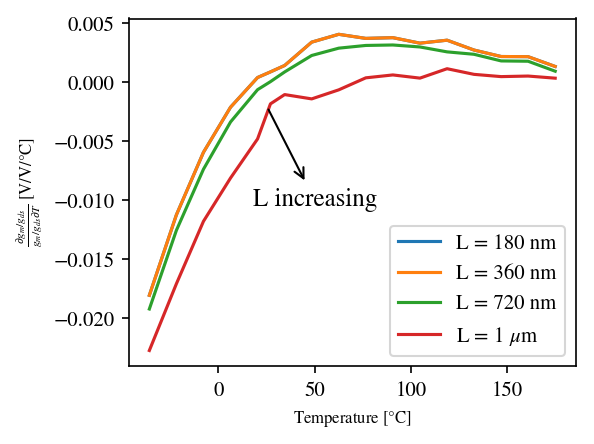
\includegraphics[width=\textwidth]{sAv_nel_T_2e-07}
		\resizebox {\textwidth} {!} {
			%% Creator: Matplotlib, PGF backend
%%
%% To include the figure in your LaTeX document, write
%%   \input{<filename>.pgf}
%%
%% Make sure the required packages are loaded in your preamble
%%   \usepackage{pgf}
%%
%% Figures using additional raster images can only be included by \input if
%% they are in the same directory as the main LaTeX file. For loading figures
%% from other directories you can use the `import` package
%%   \usepackage{import}
%% and then include the figures with
%%   \import{<path to file>}{<filename>.pgf}
%%
%% Matplotlib used the following preamble
%%   \usepackage{gensymb}
%%   \usepackage[utf8x]{inputenc}
%%   \usepackage[T1]{fontenc}
%%
\begingroup%
\makeatletter%
\begin{pgfpicture}%
\pgfpathrectangle{\pgfpointorigin}{\pgfqpoint{3.840000in}{2.840000in}}%
\pgfusepath{use as bounding box, clip}%
\begin{pgfscope}%
\pgfsetbuttcap%
\pgfsetmiterjoin%
\definecolor{currentfill}{rgb}{1.000000,1.000000,1.000000}%
\pgfsetfillcolor{currentfill}%
\pgfsetlinewidth{0.000000pt}%
\definecolor{currentstroke}{rgb}{1.000000,1.000000,1.000000}%
\pgfsetstrokecolor{currentstroke}%
\pgfsetdash{}{0pt}%
\pgfpathmoveto{\pgfqpoint{0.000000in}{0.000000in}}%
\pgfpathlineto{\pgfqpoint{3.840000in}{0.000000in}}%
\pgfpathlineto{\pgfqpoint{3.840000in}{2.840000in}}%
\pgfpathlineto{\pgfqpoint{0.000000in}{2.840000in}}%
\pgfpathclose%
\pgfusepath{fill}%
\end{pgfscope}%
\begin{pgfscope}%
\pgfsetbuttcap%
\pgfsetmiterjoin%
\definecolor{currentfill}{rgb}{1.000000,1.000000,1.000000}%
\pgfsetfillcolor{currentfill}%
\pgfsetlinewidth{0.000000pt}%
\definecolor{currentstroke}{rgb}{0.000000,0.000000,0.000000}%
\pgfsetstrokecolor{currentstroke}%
\pgfsetstrokeopacity{0.000000}%
\pgfsetdash{}{0pt}%
\pgfpathmoveto{\pgfqpoint{1.248136in}{0.596026in}}%
\pgfpathlineto{\pgfqpoint{3.716667in}{0.596026in}}%
\pgfpathlineto{\pgfqpoint{3.716667in}{2.716667in}}%
\pgfpathlineto{\pgfqpoint{1.248136in}{2.716667in}}%
\pgfpathclose%
\pgfusepath{fill}%
\end{pgfscope}%
\begin{pgfscope}%
\pgfsetbuttcap%
\pgfsetroundjoin%
\definecolor{currentfill}{rgb}{0.000000,0.000000,0.000000}%
\pgfsetfillcolor{currentfill}%
\pgfsetlinewidth{0.803000pt}%
\definecolor{currentstroke}{rgb}{0.000000,0.000000,0.000000}%
\pgfsetstrokecolor{currentstroke}%
\pgfsetdash{}{0pt}%
\pgfsys@defobject{currentmarker}{\pgfqpoint{0.000000in}{-0.048611in}}{\pgfqpoint{0.000000in}{0.000000in}}{%
\pgfpathmoveto{\pgfqpoint{0.000000in}{0.000000in}}%
\pgfpathlineto{\pgfqpoint{0.000000in}{-0.048611in}}%
\pgfusepath{stroke,fill}%
}%
\begin{pgfscope}%
\pgfsys@transformshift{1.742695in}{0.596026in}%
\pgfsys@useobject{currentmarker}{}%
\end{pgfscope}%
\end{pgfscope}%
\begin{pgfscope}%
\pgftext[x=1.742695in,y=0.498804in,,top]{\fontsize{14.000000}{16.800000}\selectfont \(\displaystyle 0\)}%
\end{pgfscope}%
\begin{pgfscope}%
\pgfsetbuttcap%
\pgfsetroundjoin%
\definecolor{currentfill}{rgb}{0.000000,0.000000,0.000000}%
\pgfsetfillcolor{currentfill}%
\pgfsetlinewidth{0.803000pt}%
\definecolor{currentstroke}{rgb}{0.000000,0.000000,0.000000}%
\pgfsetstrokecolor{currentstroke}%
\pgfsetdash{}{0pt}%
\pgfsys@defobject{currentmarker}{\pgfqpoint{0.000000in}{-0.048611in}}{\pgfqpoint{0.000000in}{0.000000in}}{%
\pgfpathmoveto{\pgfqpoint{0.000000in}{0.000000in}}%
\pgfpathlineto{\pgfqpoint{0.000000in}{-0.048611in}}%
\pgfusepath{stroke,fill}%
}%
\begin{pgfscope}%
\pgfsys@transformshift{2.806561in}{0.596026in}%
\pgfsys@useobject{currentmarker}{}%
\end{pgfscope}%
\end{pgfscope}%
\begin{pgfscope}%
\pgftext[x=2.806561in,y=0.498804in,,top]{\fontsize{14.000000}{16.800000}\selectfont \(\displaystyle 100\)}%
\end{pgfscope}%
\begin{pgfscope}%
\pgftext[x=2.482401in,y=0.266626in,,top]{\fontsize{12.000000}{14.400000}\selectfont Temperature [\(\displaystyle \degree\)C]}%
\end{pgfscope}%
\begin{pgfscope}%
\pgfsetbuttcap%
\pgfsetroundjoin%
\definecolor{currentfill}{rgb}{0.000000,0.000000,0.000000}%
\pgfsetfillcolor{currentfill}%
\pgfsetlinewidth{0.803000pt}%
\definecolor{currentstroke}{rgb}{0.000000,0.000000,0.000000}%
\pgfsetstrokecolor{currentstroke}%
\pgfsetdash{}{0pt}%
\pgfsys@defobject{currentmarker}{\pgfqpoint{-0.048611in}{0.000000in}}{\pgfqpoint{0.000000in}{0.000000in}}{%
\pgfpathmoveto{\pgfqpoint{0.000000in}{0.000000in}}%
\pgfpathlineto{\pgfqpoint{-0.048611in}{0.000000in}}%
\pgfusepath{stroke,fill}%
}%
\begin{pgfscope}%
\pgfsys@transformshift{1.248136in}{0.883980in}%
\pgfsys@useobject{currentmarker}{}%
\end{pgfscope}%
\end{pgfscope}%
\begin{pgfscope}%
\pgftext[x=0.549299in,y=0.815114in,left,base]{\fontsize{14.000000}{16.800000}\selectfont \(\displaystyle -0.015\)}%
\end{pgfscope}%
\begin{pgfscope}%
\pgfsetbuttcap%
\pgfsetroundjoin%
\definecolor{currentfill}{rgb}{0.000000,0.000000,0.000000}%
\pgfsetfillcolor{currentfill}%
\pgfsetlinewidth{0.803000pt}%
\definecolor{currentstroke}{rgb}{0.000000,0.000000,0.000000}%
\pgfsetstrokecolor{currentstroke}%
\pgfsetdash{}{0pt}%
\pgfsys@defobject{currentmarker}{\pgfqpoint{-0.048611in}{0.000000in}}{\pgfqpoint{0.000000in}{0.000000in}}{%
\pgfpathmoveto{\pgfqpoint{0.000000in}{0.000000in}}%
\pgfpathlineto{\pgfqpoint{-0.048611in}{0.000000in}}%
\pgfusepath{stroke,fill}%
}%
\begin{pgfscope}%
\pgfsys@transformshift{1.248136in}{1.346354in}%
\pgfsys@useobject{currentmarker}{}%
\end{pgfscope}%
\end{pgfscope}%
\begin{pgfscope}%
\pgftext[x=0.549299in,y=1.277488in,left,base]{\fontsize{14.000000}{16.800000}\selectfont \(\displaystyle -0.010\)}%
\end{pgfscope}%
\begin{pgfscope}%
\pgfsetbuttcap%
\pgfsetroundjoin%
\definecolor{currentfill}{rgb}{0.000000,0.000000,0.000000}%
\pgfsetfillcolor{currentfill}%
\pgfsetlinewidth{0.803000pt}%
\definecolor{currentstroke}{rgb}{0.000000,0.000000,0.000000}%
\pgfsetstrokecolor{currentstroke}%
\pgfsetdash{}{0pt}%
\pgfsys@defobject{currentmarker}{\pgfqpoint{-0.048611in}{0.000000in}}{\pgfqpoint{0.000000in}{0.000000in}}{%
\pgfpathmoveto{\pgfqpoint{0.000000in}{0.000000in}}%
\pgfpathlineto{\pgfqpoint{-0.048611in}{0.000000in}}%
\pgfusepath{stroke,fill}%
}%
\begin{pgfscope}%
\pgfsys@transformshift{1.248136in}{1.808728in}%
\pgfsys@useobject{currentmarker}{}%
\end{pgfscope}%
\end{pgfscope}%
\begin{pgfscope}%
\pgftext[x=0.549299in,y=1.739862in,left,base]{\fontsize{14.000000}{16.800000}\selectfont \(\displaystyle -0.005\)}%
\end{pgfscope}%
\begin{pgfscope}%
\pgfsetbuttcap%
\pgfsetroundjoin%
\definecolor{currentfill}{rgb}{0.000000,0.000000,0.000000}%
\pgfsetfillcolor{currentfill}%
\pgfsetlinewidth{0.803000pt}%
\definecolor{currentstroke}{rgb}{0.000000,0.000000,0.000000}%
\pgfsetstrokecolor{currentstroke}%
\pgfsetdash{}{0pt}%
\pgfsys@defobject{currentmarker}{\pgfqpoint{-0.048611in}{0.000000in}}{\pgfqpoint{0.000000in}{0.000000in}}{%
\pgfpathmoveto{\pgfqpoint{0.000000in}{0.000000in}}%
\pgfpathlineto{\pgfqpoint{-0.048611in}{0.000000in}}%
\pgfusepath{stroke,fill}%
}%
\begin{pgfscope}%
\pgfsys@transformshift{1.248136in}{2.271101in}%
\pgfsys@useobject{currentmarker}{}%
\end{pgfscope}%
\end{pgfscope}%
\begin{pgfscope}%
\pgftext[x=0.704854in,y=2.202235in,left,base]{\fontsize{14.000000}{16.800000}\selectfont \(\displaystyle 0.000\)}%
\end{pgfscope}%
\begin{pgfscope}%
\pgftext[x=0.493743in,y=1.656346in,,bottom,rotate=90.000000]{\fontsize{12.000000}{14.400000}\selectfont \(\displaystyle \frac{\partial g_m/g_{ds}}{g_m/g_{ds}\partial T}\) [V/V/\(\displaystyle \degree\)C]}%
\end{pgfscope}%
\begin{pgfscope}%
\pgfpathrectangle{\pgfqpoint{1.248136in}{0.596026in}}{\pgfqpoint{2.468531in}{2.120641in}} %
\pgfusepath{clip}%
\pgfsetrectcap%
\pgfsetroundjoin%
\pgfsetlinewidth{1.505625pt}%
\definecolor{currentstroke}{rgb}{0.121569,0.466667,0.705882}%
\pgfsetstrokecolor{currentstroke}%
\pgfsetdash{}{0pt}%
\pgfpathmoveto{\pgfqpoint{1.360342in}{1.232360in}}%
\pgfpathlineto{\pgfqpoint{1.509921in}{1.232360in}}%
\pgfpathlineto{\pgfqpoint{1.659586in}{1.722341in}}%
\pgfpathlineto{\pgfqpoint{1.809187in}{2.075350in}}%
\pgfpathlineto{\pgfqpoint{1.958766in}{2.308122in}}%
\pgfpathlineto{\pgfqpoint{2.029939in}{2.352186in}}%
\pgfpathlineto{\pgfqpoint{2.108452in}{2.402365in}}%
\pgfpathlineto{\pgfqpoint{2.258032in}{2.585261in}}%
\pgfpathlineto{\pgfqpoint{2.407611in}{2.614545in}}%
\pgfpathlineto{\pgfqpoint{2.557191in}{2.620274in}}%
\pgfpathlineto{\pgfqpoint{2.706771in}{2.614545in}}%
\pgfpathlineto{\pgfqpoint{2.856563in}{2.600445in}}%
\pgfpathlineto{\pgfqpoint{3.006568in}{2.577177in}}%
\pgfpathlineto{\pgfqpoint{3.155509in}{2.523293in}}%
\pgfpathlineto{\pgfqpoint{3.305514in}{2.472624in}}%
\pgfpathlineto{\pgfqpoint{3.454456in}{2.471459in}}%
\pgfpathlineto{\pgfqpoint{3.604461in}{2.394654in}}%
\pgfusepath{stroke}%
\end{pgfscope}%
\begin{pgfscope}%
\pgfpathrectangle{\pgfqpoint{1.248136in}{0.596026in}}{\pgfqpoint{2.468531in}{2.120641in}} %
\pgfusepath{clip}%
\pgfsetrectcap%
\pgfsetroundjoin%
\pgfsetlinewidth{1.505625pt}%
\definecolor{currentstroke}{rgb}{1.000000,0.498039,0.054902}%
\pgfsetstrokecolor{currentstroke}%
\pgfsetdash{}{0pt}%
\pgfpathmoveto{\pgfqpoint{1.360342in}{1.232360in}}%
\pgfpathlineto{\pgfqpoint{1.509921in}{1.232360in}}%
\pgfpathlineto{\pgfqpoint{1.659586in}{1.722341in}}%
\pgfpathlineto{\pgfqpoint{1.809187in}{2.075350in}}%
\pgfpathlineto{\pgfqpoint{1.958766in}{2.308122in}}%
\pgfpathlineto{\pgfqpoint{2.029939in}{2.352186in}}%
\pgfpathlineto{\pgfqpoint{2.108452in}{2.402365in}}%
\pgfpathlineto{\pgfqpoint{2.258032in}{2.585261in}}%
\pgfpathlineto{\pgfqpoint{2.407611in}{2.614545in}}%
\pgfpathlineto{\pgfqpoint{2.557191in}{2.620274in}}%
\pgfpathlineto{\pgfqpoint{2.706771in}{2.614545in}}%
\pgfpathlineto{\pgfqpoint{2.856563in}{2.600445in}}%
\pgfpathlineto{\pgfqpoint{3.006568in}{2.577177in}}%
\pgfpathlineto{\pgfqpoint{3.155509in}{2.523293in}}%
\pgfpathlineto{\pgfqpoint{3.305514in}{2.472624in}}%
\pgfpathlineto{\pgfqpoint{3.454456in}{2.471459in}}%
\pgfpathlineto{\pgfqpoint{3.604461in}{2.394654in}}%
\pgfusepath{stroke}%
\end{pgfscope}%
\begin{pgfscope}%
\pgfpathrectangle{\pgfqpoint{1.248136in}{0.596026in}}{\pgfqpoint{2.468531in}{2.120641in}} %
\pgfusepath{clip}%
\pgfsetrectcap%
\pgfsetroundjoin%
\pgfsetlinewidth{1.505625pt}%
\definecolor{currentstroke}{rgb}{0.172549,0.627451,0.172549}%
\pgfsetstrokecolor{currentstroke}%
\pgfsetdash{}{0pt}%
\pgfpathmoveto{\pgfqpoint{1.360342in}{1.110986in}}%
\pgfpathlineto{\pgfqpoint{1.509921in}{1.110986in}}%
\pgfpathlineto{\pgfqpoint{1.659586in}{1.589705in}}%
\pgfpathlineto{\pgfqpoint{1.809187in}{1.959788in}}%
\pgfpathlineto{\pgfqpoint{1.958766in}{2.212877in}}%
\pgfpathlineto{\pgfqpoint{2.029939in}{2.275667in}}%
\pgfpathlineto{\pgfqpoint{2.108452in}{2.351752in}}%
\pgfpathlineto{\pgfqpoint{2.258032in}{2.480717in}}%
\pgfpathlineto{\pgfqpoint{2.407611in}{2.538022in}}%
\pgfpathlineto{\pgfqpoint{2.557191in}{2.559314in}}%
\pgfpathlineto{\pgfqpoint{2.706771in}{2.559314in}}%
\pgfpathlineto{\pgfqpoint{2.856563in}{2.547455in}}%
\pgfpathlineto{\pgfqpoint{3.006568in}{2.509015in}}%
\pgfpathlineto{\pgfqpoint{3.155509in}{2.490086in}}%
\pgfpathlineto{\pgfqpoint{3.305514in}{2.438072in}}%
\pgfpathlineto{\pgfqpoint{3.454456in}{2.435620in}}%
\pgfpathlineto{\pgfqpoint{3.604461in}{2.357341in}}%
\pgfusepath{stroke}%
\end{pgfscope}%
\begin{pgfscope}%
\pgfpathrectangle{\pgfqpoint{1.248136in}{0.596026in}}{\pgfqpoint{2.468531in}{2.120641in}} %
\pgfusepath{clip}%
\pgfsetrectcap%
\pgfsetroundjoin%
\pgfsetlinewidth{1.505625pt}%
\definecolor{currentstroke}{rgb}{0.839216,0.152941,0.156863}%
\pgfsetstrokecolor{currentstroke}%
\pgfsetdash{}{0pt}%
\pgfpathmoveto{\pgfqpoint{1.360342in}{0.692419in}}%
\pgfpathlineto{\pgfqpoint{1.509921in}{0.692419in}}%
\pgfpathlineto{\pgfqpoint{1.659586in}{1.181678in}}%
\pgfpathlineto{\pgfqpoint{1.809187in}{1.520767in}}%
\pgfpathlineto{\pgfqpoint{1.958766in}{1.827192in}}%
\pgfpathlineto{\pgfqpoint{2.029939in}{2.101785in}}%
\pgfpathlineto{\pgfqpoint{2.108452in}{2.140678in}}%
\pgfpathlineto{\pgfqpoint{2.258032in}{2.174478in}}%
\pgfpathlineto{\pgfqpoint{2.407611in}{2.211547in}}%
\pgfpathlineto{\pgfqpoint{2.557191in}{2.305603in}}%
\pgfpathlineto{\pgfqpoint{2.706771in}{2.305603in}}%
\pgfpathlineto{\pgfqpoint{2.856563in}{2.328333in}}%
\pgfpathlineto{\pgfqpoint{3.006568in}{2.332887in}}%
\pgfpathlineto{\pgfqpoint{3.155509in}{2.332887in}}%
\pgfpathlineto{\pgfqpoint{3.305514in}{2.319609in}}%
\pgfpathlineto{\pgfqpoint{3.454456in}{2.315151in}}%
\pgfpathlineto{\pgfqpoint{3.604461in}{2.302952in}}%
\pgfusepath{stroke}%
\end{pgfscope}%
\begin{pgfscope}%
\pgfsetrectcap%
\pgfsetmiterjoin%
\pgfsetlinewidth{0.803000pt}%
\definecolor{currentstroke}{rgb}{0.000000,0.000000,0.000000}%
\pgfsetstrokecolor{currentstroke}%
\pgfsetdash{}{0pt}%
\pgfpathmoveto{\pgfqpoint{1.248136in}{0.596026in}}%
\pgfpathlineto{\pgfqpoint{1.248136in}{2.716667in}}%
\pgfusepath{stroke}%
\end{pgfscope}%
\begin{pgfscope}%
\pgfsetrectcap%
\pgfsetmiterjoin%
\pgfsetlinewidth{0.803000pt}%
\definecolor{currentstroke}{rgb}{0.000000,0.000000,0.000000}%
\pgfsetstrokecolor{currentstroke}%
\pgfsetdash{}{0pt}%
\pgfpathmoveto{\pgfqpoint{3.716667in}{0.596026in}}%
\pgfpathlineto{\pgfqpoint{3.716667in}{2.716667in}}%
\pgfusepath{stroke}%
\end{pgfscope}%
\begin{pgfscope}%
\pgfsetrectcap%
\pgfsetmiterjoin%
\pgfsetlinewidth{0.803000pt}%
\definecolor{currentstroke}{rgb}{0.000000,0.000000,0.000000}%
\pgfsetstrokecolor{currentstroke}%
\pgfsetdash{}{0pt}%
\pgfpathmoveto{\pgfqpoint{1.248136in}{0.596026in}}%
\pgfpathlineto{\pgfqpoint{3.716667in}{0.596026in}}%
\pgfusepath{stroke}%
\end{pgfscope}%
\begin{pgfscope}%
\pgfsetrectcap%
\pgfsetmiterjoin%
\pgfsetlinewidth{0.803000pt}%
\definecolor{currentstroke}{rgb}{0.000000,0.000000,0.000000}%
\pgfsetstrokecolor{currentstroke}%
\pgfsetdash{}{0pt}%
\pgfpathmoveto{\pgfqpoint{1.248136in}{2.716667in}}%
\pgfpathlineto{\pgfqpoint{3.716667in}{2.716667in}}%
\pgfusepath{stroke}%
\end{pgfscope}%
\begin{pgfscope}%
\pgfsetroundcap%
\pgfsetroundjoin%
\pgfsetlinewidth{1.003750pt}%
\definecolor{currentstroke}{rgb}{0.000000,0.000000,0.000000}%
\pgfsetstrokecolor{currentstroke}%
\pgfsetdash{}{0pt}%
\pgfpathmoveto{\pgfqpoint{2.351298in}{1.755229in}}%
\pgfpathquadraticcurveto{\pgfqpoint{2.195552in}{1.905651in}}{\pgfqpoint{2.028637in}{2.066860in}}%
\pgfusepath{stroke}%
\end{pgfscope}%
\begin{pgfscope}%
\pgfsetroundcap%
\pgfsetroundjoin%
\pgfsetlinewidth{1.003750pt}%
\definecolor{currentstroke}{rgb}{0.000000,0.000000,0.000000}%
\pgfsetstrokecolor{currentstroke}%
\pgfsetdash{}{0pt}%
\pgfpathmoveto{\pgfqpoint{2.326502in}{1.825519in}}%
\pgfpathlineto{\pgfqpoint{2.351298in}{1.755229in}}%
\pgfpathlineto{\pgfqpoint{2.280188in}{1.777566in}}%
\pgfusepath{stroke}%
\end{pgfscope}%
\begin{pgfscope}%
\pgftext[x=2.487401in,y=1.623778in,,]{\fontsize{12.000000}{14.400000}\selectfont L increasing}%
\end{pgfscope}%
\begin{pgfscope}%
\pgfsetbuttcap%
\pgfsetmiterjoin%
\definecolor{currentfill}{rgb}{1.000000,1.000000,1.000000}%
\pgfsetfillcolor{currentfill}%
\pgfsetfillopacity{0.800000}%
\pgfsetlinewidth{1.003750pt}%
\definecolor{currentstroke}{rgb}{0.800000,0.800000,0.800000}%
\pgfsetstrokecolor{currentstroke}%
\pgfsetstrokeopacity{0.800000}%
\pgfsetdash{}{0pt}%
\pgfpathmoveto{\pgfqpoint{2.440226in}{0.665470in}}%
\pgfpathlineto{\pgfqpoint{3.619444in}{0.665470in}}%
\pgfpathquadraticcurveto{\pgfqpoint{3.647222in}{0.665470in}}{\pgfqpoint{3.647222in}{0.693248in}}%
\pgfpathlineto{\pgfqpoint{3.647222in}{1.454031in}}%
\pgfpathquadraticcurveto{\pgfqpoint{3.647222in}{1.481809in}}{\pgfqpoint{3.619444in}{1.481809in}}%
\pgfpathlineto{\pgfqpoint{2.440226in}{1.481809in}}%
\pgfpathquadraticcurveto{\pgfqpoint{2.412448in}{1.481809in}}{\pgfqpoint{2.412448in}{1.454031in}}%
\pgfpathlineto{\pgfqpoint{2.412448in}{0.693248in}}%
\pgfpathquadraticcurveto{\pgfqpoint{2.412448in}{0.665470in}}{\pgfqpoint{2.440226in}{0.665470in}}%
\pgfpathclose%
\pgfusepath{stroke,fill}%
\end{pgfscope}%
\begin{pgfscope}%
\pgfsetrectcap%
\pgfsetroundjoin%
\pgfsetlinewidth{1.505625pt}%
\definecolor{currentstroke}{rgb}{0.121569,0.466667,0.705882}%
\pgfsetstrokecolor{currentstroke}%
\pgfsetdash{}{0pt}%
\pgfpathmoveto{\pgfqpoint{2.468003in}{1.377642in}}%
\pgfpathlineto{\pgfqpoint{2.745781in}{1.377642in}}%
\pgfusepath{stroke}%
\end{pgfscope}%
\begin{pgfscope}%
\pgftext[x=2.856892in,y=1.329031in,left,base]{\fontsize{10.000000}{12.000000}\selectfont L = 180 nm}%
\end{pgfscope}%
\begin{pgfscope}%
\pgfsetrectcap%
\pgfsetroundjoin%
\pgfsetlinewidth{1.505625pt}%
\definecolor{currentstroke}{rgb}{1.000000,0.498039,0.054902}%
\pgfsetstrokecolor{currentstroke}%
\pgfsetdash{}{0pt}%
\pgfpathmoveto{\pgfqpoint{2.468003in}{1.183976in}}%
\pgfpathlineto{\pgfqpoint{2.745781in}{1.183976in}}%
\pgfusepath{stroke}%
\end{pgfscope}%
\begin{pgfscope}%
\pgftext[x=2.856892in,y=1.135365in,left,base]{\fontsize{10.000000}{12.000000}\selectfont L = 360 nm}%
\end{pgfscope}%
\begin{pgfscope}%
\pgfsetrectcap%
\pgfsetroundjoin%
\pgfsetlinewidth{1.505625pt}%
\definecolor{currentstroke}{rgb}{0.172549,0.627451,0.172549}%
\pgfsetstrokecolor{currentstroke}%
\pgfsetdash{}{0pt}%
\pgfpathmoveto{\pgfqpoint{2.468003in}{0.990309in}}%
\pgfpathlineto{\pgfqpoint{2.745781in}{0.990309in}}%
\pgfusepath{stroke}%
\end{pgfscope}%
\begin{pgfscope}%
\pgftext[x=2.856892in,y=0.941698in,left,base]{\fontsize{10.000000}{12.000000}\selectfont L = 720 nm}%
\end{pgfscope}%
\begin{pgfscope}%
\pgfsetrectcap%
\pgfsetroundjoin%
\pgfsetlinewidth{1.505625pt}%
\definecolor{currentstroke}{rgb}{0.839216,0.152941,0.156863}%
\pgfsetstrokecolor{currentstroke}%
\pgfsetdash{}{0pt}%
\pgfpathmoveto{\pgfqpoint{2.468003in}{0.796643in}}%
\pgfpathlineto{\pgfqpoint{2.745781in}{0.796643in}}%
\pgfusepath{stroke}%
\end{pgfscope}%
\begin{pgfscope}%
\pgftext[x=2.856892in,y=0.748032in,left,base]{\fontsize{10.000000}{12.000000}\selectfont L = 1 \(\displaystyle \mu\)m}%
\end{pgfscope}%
\end{pgfpicture}%
\makeatother%
\endgroup%

		}
		\subcaption{temperature sensitivity for \(I_{DS} = 200 nA \)}
		\label{fig:Av_nel_sensitivity_wi}
	\end{subfigure}
	\begin{subfigure}[b]{0.48\textwidth}
		%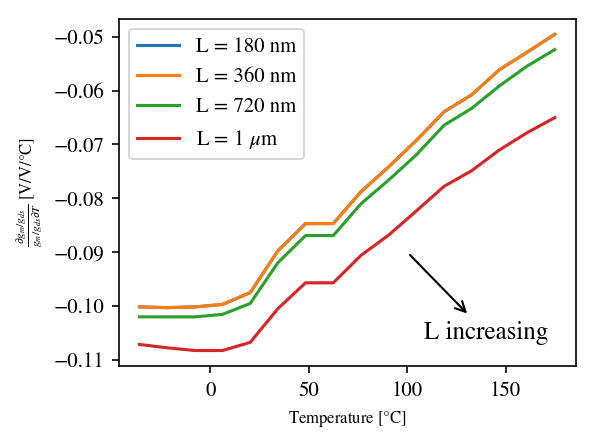
\includegraphics[width=\textwidth]{sAv_nel_T_1e-05}
		\resizebox {\textwidth} {!} {
			%% Creator: Matplotlib, PGF backend
%%
%% To include the figure in your LaTeX document, write
%%   \input{<filename>.pgf}
%%
%% Make sure the required packages are loaded in your preamble
%%   \usepackage{pgf}
%%
%% Figures using additional raster images can only be included by \input if
%% they are in the same directory as the main LaTeX file. For loading figures
%% from other directories you can use the `import` package
%%   \usepackage{import}
%% and then include the figures with
%%   \import{<path to file>}{<filename>.pgf}
%%
%% Matplotlib used the following preamble
%%   \usepackage{gensymb}
%%   \usepackage[utf8x]{inputenc}
%%   \usepackage[T1]{fontenc}
%%
\begingroup%
\makeatletter%
\begin{pgfpicture}%
\pgfpathrectangle{\pgfpointorigin}{\pgfqpoint{3.840000in}{2.840000in}}%
\pgfusepath{use as bounding box, clip}%
\begin{pgfscope}%
\pgfsetbuttcap%
\pgfsetmiterjoin%
\definecolor{currentfill}{rgb}{1.000000,1.000000,1.000000}%
\pgfsetfillcolor{currentfill}%
\pgfsetlinewidth{0.000000pt}%
\definecolor{currentstroke}{rgb}{1.000000,1.000000,1.000000}%
\pgfsetstrokecolor{currentstroke}%
\pgfsetdash{}{0pt}%
\pgfpathmoveto{\pgfqpoint{0.000000in}{0.000000in}}%
\pgfpathlineto{\pgfqpoint{3.840000in}{0.000000in}}%
\pgfpathlineto{\pgfqpoint{3.840000in}{2.840000in}}%
\pgfpathlineto{\pgfqpoint{0.000000in}{2.840000in}}%
\pgfpathclose%
\pgfusepath{fill}%
\end{pgfscope}%
\begin{pgfscope}%
\pgfsetbuttcap%
\pgfsetmiterjoin%
\definecolor{currentfill}{rgb}{1.000000,1.000000,1.000000}%
\pgfsetfillcolor{currentfill}%
\pgfsetlinewidth{0.000000pt}%
\definecolor{currentstroke}{rgb}{0.000000,0.000000,0.000000}%
\pgfsetstrokecolor{currentstroke}%
\pgfsetstrokeopacity{0.000000}%
\pgfsetdash{}{0pt}%
\pgfpathmoveto{\pgfqpoint{1.150220in}{0.596026in}}%
\pgfpathlineto{\pgfqpoint{3.716667in}{0.596026in}}%
\pgfpathlineto{\pgfqpoint{3.716667in}{2.716667in}}%
\pgfpathlineto{\pgfqpoint{1.150220in}{2.716667in}}%
\pgfpathclose%
\pgfusepath{fill}%
\end{pgfscope}%
\begin{pgfscope}%
\pgfsetbuttcap%
\pgfsetroundjoin%
\definecolor{currentfill}{rgb}{0.000000,0.000000,0.000000}%
\pgfsetfillcolor{currentfill}%
\pgfsetlinewidth{0.803000pt}%
\definecolor{currentstroke}{rgb}{0.000000,0.000000,0.000000}%
\pgfsetstrokecolor{currentstroke}%
\pgfsetdash{}{0pt}%
\pgfsys@defobject{currentmarker}{\pgfqpoint{0.000000in}{-0.048611in}}{\pgfqpoint{0.000000in}{0.000000in}}{%
\pgfpathmoveto{\pgfqpoint{0.000000in}{0.000000in}}%
\pgfpathlineto{\pgfqpoint{0.000000in}{-0.048611in}}%
\pgfusepath{stroke,fill}%
}%
\begin{pgfscope}%
\pgfsys@transformshift{1.664397in}{0.596026in}%
\pgfsys@useobject{currentmarker}{}%
\end{pgfscope}%
\end{pgfscope}%
\begin{pgfscope}%
\pgftext[x=1.664397in,y=0.498804in,,top]{\fontsize{14.000000}{16.800000}\selectfont \(\displaystyle 0\)}%
\end{pgfscope}%
\begin{pgfscope}%
\pgfsetbuttcap%
\pgfsetroundjoin%
\definecolor{currentfill}{rgb}{0.000000,0.000000,0.000000}%
\pgfsetfillcolor{currentfill}%
\pgfsetlinewidth{0.803000pt}%
\definecolor{currentstroke}{rgb}{0.000000,0.000000,0.000000}%
\pgfsetstrokecolor{currentstroke}%
\pgfsetdash{}{0pt}%
\pgfsys@defobject{currentmarker}{\pgfqpoint{0.000000in}{-0.048611in}}{\pgfqpoint{0.000000in}{0.000000in}}{%
\pgfpathmoveto{\pgfqpoint{0.000000in}{0.000000in}}%
\pgfpathlineto{\pgfqpoint{0.000000in}{-0.048611in}}%
\pgfusepath{stroke,fill}%
}%
\begin{pgfscope}%
\pgfsys@transformshift{2.770461in}{0.596026in}%
\pgfsys@useobject{currentmarker}{}%
\end{pgfscope}%
\end{pgfscope}%
\begin{pgfscope}%
\pgftext[x=2.770461in,y=0.498804in,,top]{\fontsize{14.000000}{16.800000}\selectfont \(\displaystyle 100\)}%
\end{pgfscope}%
\begin{pgfscope}%
\pgftext[x=2.433444in,y=0.266626in,,top]{\fontsize{12.000000}{14.400000}\selectfont Temperature [\(\displaystyle \degree\)C]}%
\end{pgfscope}%
\begin{pgfscope}%
\pgfsetbuttcap%
\pgfsetroundjoin%
\definecolor{currentfill}{rgb}{0.000000,0.000000,0.000000}%
\pgfsetfillcolor{currentfill}%
\pgfsetlinewidth{0.803000pt}%
\definecolor{currentstroke}{rgb}{0.000000,0.000000,0.000000}%
\pgfsetstrokecolor{currentstroke}%
\pgfsetdash{}{0pt}%
\pgfsys@defobject{currentmarker}{\pgfqpoint{-0.048611in}{0.000000in}}{\pgfqpoint{0.000000in}{0.000000in}}{%
\pgfpathmoveto{\pgfqpoint{0.000000in}{0.000000in}}%
\pgfpathlineto{\pgfqpoint{-0.048611in}{0.000000in}}%
\pgfusepath{stroke,fill}%
}%
\begin{pgfscope}%
\pgfsys@transformshift{1.150220in}{0.965199in}%
\pgfsys@useobject{currentmarker}{}%
\end{pgfscope}%
\end{pgfscope}%
\begin{pgfscope}%
\pgftext[x=0.549299in,y=0.896333in,left,base]{\fontsize{14.000000}{16.800000}\selectfont \(\displaystyle -0.10\)}%
\end{pgfscope}%
\begin{pgfscope}%
\pgfsetbuttcap%
\pgfsetroundjoin%
\definecolor{currentfill}{rgb}{0.000000,0.000000,0.000000}%
\pgfsetfillcolor{currentfill}%
\pgfsetlinewidth{0.803000pt}%
\definecolor{currentstroke}{rgb}{0.000000,0.000000,0.000000}%
\pgfsetstrokecolor{currentstroke}%
\pgfsetdash{}{0pt}%
\pgfsys@defobject{currentmarker}{\pgfqpoint{-0.048611in}{0.000000in}}{\pgfqpoint{0.000000in}{0.000000in}}{%
\pgfpathmoveto{\pgfqpoint{0.000000in}{0.000000in}}%
\pgfpathlineto{\pgfqpoint{-0.048611in}{0.000000in}}%
\pgfusepath{stroke,fill}%
}%
\begin{pgfscope}%
\pgfsys@transformshift{1.150220in}{1.621290in}%
\pgfsys@useobject{currentmarker}{}%
\end{pgfscope}%
\end{pgfscope}%
\begin{pgfscope}%
\pgftext[x=0.549299in,y=1.552424in,left,base]{\fontsize{14.000000}{16.800000}\selectfont \(\displaystyle -0.08\)}%
\end{pgfscope}%
\begin{pgfscope}%
\pgfsetbuttcap%
\pgfsetroundjoin%
\definecolor{currentfill}{rgb}{0.000000,0.000000,0.000000}%
\pgfsetfillcolor{currentfill}%
\pgfsetlinewidth{0.803000pt}%
\definecolor{currentstroke}{rgb}{0.000000,0.000000,0.000000}%
\pgfsetstrokecolor{currentstroke}%
\pgfsetdash{}{0pt}%
\pgfsys@defobject{currentmarker}{\pgfqpoint{-0.048611in}{0.000000in}}{\pgfqpoint{0.000000in}{0.000000in}}{%
\pgfpathmoveto{\pgfqpoint{0.000000in}{0.000000in}}%
\pgfpathlineto{\pgfqpoint{-0.048611in}{0.000000in}}%
\pgfusepath{stroke,fill}%
}%
\begin{pgfscope}%
\pgfsys@transformshift{1.150220in}{2.277381in}%
\pgfsys@useobject{currentmarker}{}%
\end{pgfscope}%
\end{pgfscope}%
\begin{pgfscope}%
\pgftext[x=0.549299in,y=2.208515in,left,base]{\fontsize{14.000000}{16.800000}\selectfont \(\displaystyle -0.06\)}%
\end{pgfscope}%
\begin{pgfscope}%
\pgftext[x=0.493743in,y=1.656346in,,bottom,rotate=90.000000]{\fontsize{12.000000}{14.400000}\selectfont \(\displaystyle \frac{\partial g_m/g_{ds}}{g_m/g_{ds}\partial T}\) [V/V/\(\displaystyle \degree\)C]}%
\end{pgfscope}%
\begin{pgfscope}%
\pgfpathrectangle{\pgfqpoint{1.150220in}{0.596026in}}{\pgfqpoint{2.566446in}{2.120641in}} %
\pgfusepath{clip}%
\pgfsetrectcap%
\pgfsetroundjoin%
\pgfsetlinewidth{1.505625pt}%
\definecolor{currentstroke}{rgb}{0.121569,0.466667,0.705882}%
\pgfsetstrokecolor{currentstroke}%
\pgfsetdash{}{0pt}%
\pgfpathmoveto{\pgfqpoint{1.266877in}{0.958232in}}%
\pgfpathlineto{\pgfqpoint{1.422390in}{0.953838in}}%
\pgfpathlineto{\pgfqpoint{1.577991in}{0.958232in}}%
\pgfpathlineto{\pgfqpoint{1.733526in}{0.973374in}}%
\pgfpathlineto{\pgfqpoint{1.889038in}{1.045341in}}%
\pgfpathlineto{\pgfqpoint{2.044662in}{1.300428in}}%
\pgfpathlineto{\pgfqpoint{2.200174in}{1.466245in}}%
\pgfpathlineto{\pgfqpoint{2.355687in}{1.466245in}}%
\pgfpathlineto{\pgfqpoint{2.511200in}{1.660475in}}%
\pgfpathlineto{\pgfqpoint{2.666713in}{1.811955in}}%
\pgfpathlineto{\pgfqpoint{2.822447in}{1.973595in}}%
\pgfpathlineto{\pgfqpoint{2.978402in}{2.148024in}}%
\pgfpathlineto{\pgfqpoint{3.133251in}{2.251533in}}%
\pgfpathlineto{\pgfqpoint{3.289206in}{2.404516in}}%
\pgfpathlineto{\pgfqpoint{3.444055in}{2.510623in}}%
\pgfpathlineto{\pgfqpoint{3.600010in}{2.620274in}}%
\pgfusepath{stroke}%
\end{pgfscope}%
\begin{pgfscope}%
\pgfpathrectangle{\pgfqpoint{1.150220in}{0.596026in}}{\pgfqpoint{2.566446in}{2.120641in}} %
\pgfusepath{clip}%
\pgfsetrectcap%
\pgfsetroundjoin%
\pgfsetlinewidth{1.505625pt}%
\definecolor{currentstroke}{rgb}{1.000000,0.498039,0.054902}%
\pgfsetstrokecolor{currentstroke}%
\pgfsetdash{}{0pt}%
\pgfpathmoveto{\pgfqpoint{1.266877in}{0.958232in}}%
\pgfpathlineto{\pgfqpoint{1.422390in}{0.953838in}}%
\pgfpathlineto{\pgfqpoint{1.577991in}{0.958232in}}%
\pgfpathlineto{\pgfqpoint{1.733526in}{0.973374in}}%
\pgfpathlineto{\pgfqpoint{1.889038in}{1.045341in}}%
\pgfpathlineto{\pgfqpoint{2.044662in}{1.300428in}}%
\pgfpathlineto{\pgfqpoint{2.200174in}{1.466245in}}%
\pgfpathlineto{\pgfqpoint{2.355687in}{1.466245in}}%
\pgfpathlineto{\pgfqpoint{2.511200in}{1.660475in}}%
\pgfpathlineto{\pgfqpoint{2.666713in}{1.811955in}}%
\pgfpathlineto{\pgfqpoint{2.822447in}{1.973595in}}%
\pgfpathlineto{\pgfqpoint{2.978402in}{2.148024in}}%
\pgfpathlineto{\pgfqpoint{3.133251in}{2.251533in}}%
\pgfpathlineto{\pgfqpoint{3.289206in}{2.404516in}}%
\pgfpathlineto{\pgfqpoint{3.444055in}{2.510623in}}%
\pgfpathlineto{\pgfqpoint{3.600010in}{2.620274in}}%
\pgfusepath{stroke}%
\end{pgfscope}%
\begin{pgfscope}%
\pgfpathrectangle{\pgfqpoint{1.150220in}{0.596026in}}{\pgfqpoint{2.566446in}{2.120641in}} %
\pgfusepath{clip}%
\pgfsetrectcap%
\pgfsetroundjoin%
\pgfsetlinewidth{1.505625pt}%
\definecolor{currentstroke}{rgb}{0.172549,0.627451,0.172549}%
\pgfsetstrokecolor{currentstroke}%
\pgfsetdash{}{0pt}%
\pgfpathmoveto{\pgfqpoint{1.266877in}{0.897693in}}%
\pgfpathlineto{\pgfqpoint{1.422390in}{0.897420in}}%
\pgfpathlineto{\pgfqpoint{1.577991in}{0.897420in}}%
\pgfpathlineto{\pgfqpoint{1.733526in}{0.912753in}}%
\pgfpathlineto{\pgfqpoint{1.889038in}{0.979180in}}%
\pgfpathlineto{\pgfqpoint{2.044662in}{1.227703in}}%
\pgfpathlineto{\pgfqpoint{2.200174in}{1.393239in}}%
\pgfpathlineto{\pgfqpoint{2.355687in}{1.393239in}}%
\pgfpathlineto{\pgfqpoint{2.511200in}{1.587077in}}%
\pgfpathlineto{\pgfqpoint{2.666713in}{1.731480in}}%
\pgfpathlineto{\pgfqpoint{2.822447in}{1.885231in}}%
\pgfpathlineto{\pgfqpoint{2.978402in}{2.066051in}}%
\pgfpathlineto{\pgfqpoint{3.133251in}{2.168705in}}%
\pgfpathlineto{\pgfqpoint{3.289206in}{2.305799in}}%
\pgfpathlineto{\pgfqpoint{3.444055in}{2.425905in}}%
\pgfpathlineto{\pgfqpoint{3.600010in}{2.527129in}}%
\pgfusepath{stroke}%
\end{pgfscope}%
\begin{pgfscope}%
\pgfpathrectangle{\pgfqpoint{1.150220in}{0.596026in}}{\pgfqpoint{2.566446in}{2.120641in}} %
\pgfusepath{clip}%
\pgfsetrectcap%
\pgfsetroundjoin%
\pgfsetlinewidth{1.505625pt}%
\definecolor{currentstroke}{rgb}{0.839216,0.152941,0.156863}%
\pgfsetstrokecolor{currentstroke}%
\pgfsetdash{}{0pt}%
\pgfpathmoveto{\pgfqpoint{1.266877in}{0.729309in}}%
\pgfpathlineto{\pgfqpoint{1.422390in}{0.708883in}}%
\pgfpathlineto{\pgfqpoint{1.577991in}{0.692419in}}%
\pgfpathlineto{\pgfqpoint{1.733526in}{0.692419in}}%
\pgfpathlineto{\pgfqpoint{1.889038in}{0.742064in}}%
\pgfpathlineto{\pgfqpoint{2.044662in}{0.947643in}}%
\pgfpathlineto{\pgfqpoint{2.200174in}{1.105211in}}%
\pgfpathlineto{\pgfqpoint{2.355687in}{1.105211in}}%
\pgfpathlineto{\pgfqpoint{2.511200in}{1.272362in}}%
\pgfpathlineto{\pgfqpoint{2.666713in}{1.395954in}}%
\pgfpathlineto{\pgfqpoint{2.822447in}{1.543611in}}%
\pgfpathlineto{\pgfqpoint{2.978402in}{1.693487in}}%
\pgfpathlineto{\pgfqpoint{3.133251in}{1.788672in}}%
\pgfpathlineto{\pgfqpoint{3.289206in}{1.915364in}}%
\pgfpathlineto{\pgfqpoint{3.444055in}{2.020149in}}%
\pgfpathlineto{\pgfqpoint{3.600010in}{2.112178in}}%
\pgfusepath{stroke}%
\end{pgfscope}%
\begin{pgfscope}%
\pgfsetrectcap%
\pgfsetmiterjoin%
\pgfsetlinewidth{0.803000pt}%
\definecolor{currentstroke}{rgb}{0.000000,0.000000,0.000000}%
\pgfsetstrokecolor{currentstroke}%
\pgfsetdash{}{0pt}%
\pgfpathmoveto{\pgfqpoint{1.150220in}{0.596026in}}%
\pgfpathlineto{\pgfqpoint{1.150220in}{2.716667in}}%
\pgfusepath{stroke}%
\end{pgfscope}%
\begin{pgfscope}%
\pgfsetrectcap%
\pgfsetmiterjoin%
\pgfsetlinewidth{0.803000pt}%
\definecolor{currentstroke}{rgb}{0.000000,0.000000,0.000000}%
\pgfsetstrokecolor{currentstroke}%
\pgfsetdash{}{0pt}%
\pgfpathmoveto{\pgfqpoint{3.716667in}{0.596026in}}%
\pgfpathlineto{\pgfqpoint{3.716667in}{2.716667in}}%
\pgfusepath{stroke}%
\end{pgfscope}%
\begin{pgfscope}%
\pgfsetrectcap%
\pgfsetmiterjoin%
\pgfsetlinewidth{0.803000pt}%
\definecolor{currentstroke}{rgb}{0.000000,0.000000,0.000000}%
\pgfsetstrokecolor{currentstroke}%
\pgfsetdash{}{0pt}%
\pgfpathmoveto{\pgfqpoint{1.150220in}{0.596026in}}%
\pgfpathlineto{\pgfqpoint{3.716667in}{0.596026in}}%
\pgfusepath{stroke}%
\end{pgfscope}%
\begin{pgfscope}%
\pgfsetrectcap%
\pgfsetmiterjoin%
\pgfsetlinewidth{0.803000pt}%
\definecolor{currentstroke}{rgb}{0.000000,0.000000,0.000000}%
\pgfsetstrokecolor{currentstroke}%
\pgfsetdash{}{0pt}%
\pgfpathmoveto{\pgfqpoint{1.150220in}{2.716667in}}%
\pgfpathlineto{\pgfqpoint{3.716667in}{2.716667in}}%
\pgfusepath{stroke}%
\end{pgfscope}%
\begin{pgfscope}%
\pgfsetroundcap%
\pgfsetroundjoin%
\pgfsetlinewidth{1.003750pt}%
\definecolor{currentstroke}{rgb}{0.000000,0.000000,0.000000}%
\pgfsetstrokecolor{currentstroke}%
\pgfsetdash{}{0pt}%
\pgfpathmoveto{\pgfqpoint{3.092766in}{0.934776in}}%
\pgfpathquadraticcurveto{\pgfqpoint{2.946095in}{1.097905in}}{\pgfqpoint{2.789041in}{1.272580in}}%
\pgfusepath{stroke}%
\end{pgfscope}%
\begin{pgfscope}%
\pgfsetroundcap%
\pgfsetroundjoin%
\pgfsetlinewidth{1.003750pt}%
\definecolor{currentstroke}{rgb}{0.000000,0.000000,0.000000}%
\pgfsetstrokecolor{currentstroke}%
\pgfsetdash{}{0pt}%
\pgfpathmoveto{\pgfqpoint{3.072980in}{1.006637in}}%
\pgfpathlineto{\pgfqpoint{3.092766in}{0.934776in}}%
\pgfpathlineto{\pgfqpoint{3.023405in}{0.962064in}}%
\pgfusepath{stroke}%
\end{pgfscope}%
\begin{pgfscope}%
\pgftext[x=3.212887in,y=0.801176in,,]{\fontsize{12.000000}{14.400000}\selectfont L increasing}%
\end{pgfscope}%
\begin{pgfscope}%
\pgfsetbuttcap%
\pgfsetmiterjoin%
\definecolor{currentfill}{rgb}{1.000000,1.000000,1.000000}%
\pgfsetfillcolor{currentfill}%
\pgfsetfillopacity{0.800000}%
\pgfsetlinewidth{1.003750pt}%
\definecolor{currentstroke}{rgb}{0.800000,0.800000,0.800000}%
\pgfsetstrokecolor{currentstroke}%
\pgfsetstrokeopacity{0.800000}%
\pgfsetdash{}{0pt}%
\pgfpathmoveto{\pgfqpoint{1.247443in}{1.830884in}}%
\pgfpathlineto{\pgfqpoint{2.426661in}{1.830884in}}%
\pgfpathquadraticcurveto{\pgfqpoint{2.454439in}{1.830884in}}{\pgfqpoint{2.454439in}{1.858662in}}%
\pgfpathlineto{\pgfqpoint{2.454439in}{2.619444in}}%
\pgfpathquadraticcurveto{\pgfqpoint{2.454439in}{2.647222in}}{\pgfqpoint{2.426661in}{2.647222in}}%
\pgfpathlineto{\pgfqpoint{1.247443in}{2.647222in}}%
\pgfpathquadraticcurveto{\pgfqpoint{1.219665in}{2.647222in}}{\pgfqpoint{1.219665in}{2.619444in}}%
\pgfpathlineto{\pgfqpoint{1.219665in}{1.858662in}}%
\pgfpathquadraticcurveto{\pgfqpoint{1.219665in}{1.830884in}}{\pgfqpoint{1.247443in}{1.830884in}}%
\pgfpathclose%
\pgfusepath{stroke,fill}%
\end{pgfscope}%
\begin{pgfscope}%
\pgfsetrectcap%
\pgfsetroundjoin%
\pgfsetlinewidth{1.505625pt}%
\definecolor{currentstroke}{rgb}{0.121569,0.466667,0.705882}%
\pgfsetstrokecolor{currentstroke}%
\pgfsetdash{}{0pt}%
\pgfpathmoveto{\pgfqpoint{1.275220in}{2.543056in}}%
\pgfpathlineto{\pgfqpoint{1.552998in}{2.543056in}}%
\pgfusepath{stroke}%
\end{pgfscope}%
\begin{pgfscope}%
\pgftext[x=1.664109in,y=2.494444in,left,base]{\fontsize{10.000000}{12.000000}\selectfont L = 180 nm}%
\end{pgfscope}%
\begin{pgfscope}%
\pgfsetrectcap%
\pgfsetroundjoin%
\pgfsetlinewidth{1.505625pt}%
\definecolor{currentstroke}{rgb}{1.000000,0.498039,0.054902}%
\pgfsetstrokecolor{currentstroke}%
\pgfsetdash{}{0pt}%
\pgfpathmoveto{\pgfqpoint{1.275220in}{2.349389in}}%
\pgfpathlineto{\pgfqpoint{1.552998in}{2.349389in}}%
\pgfusepath{stroke}%
\end{pgfscope}%
\begin{pgfscope}%
\pgftext[x=1.664109in,y=2.300778in,left,base]{\fontsize{10.000000}{12.000000}\selectfont L = 360 nm}%
\end{pgfscope}%
\begin{pgfscope}%
\pgfsetrectcap%
\pgfsetroundjoin%
\pgfsetlinewidth{1.505625pt}%
\definecolor{currentstroke}{rgb}{0.172549,0.627451,0.172549}%
\pgfsetstrokecolor{currentstroke}%
\pgfsetdash{}{0pt}%
\pgfpathmoveto{\pgfqpoint{1.275220in}{2.155723in}}%
\pgfpathlineto{\pgfqpoint{1.552998in}{2.155723in}}%
\pgfusepath{stroke}%
\end{pgfscope}%
\begin{pgfscope}%
\pgftext[x=1.664109in,y=2.107112in,left,base]{\fontsize{10.000000}{12.000000}\selectfont L = 720 nm}%
\end{pgfscope}%
\begin{pgfscope}%
\pgfsetrectcap%
\pgfsetroundjoin%
\pgfsetlinewidth{1.505625pt}%
\definecolor{currentstroke}{rgb}{0.839216,0.152941,0.156863}%
\pgfsetstrokecolor{currentstroke}%
\pgfsetdash{}{0pt}%
\pgfpathmoveto{\pgfqpoint{1.275220in}{1.962057in}}%
\pgfpathlineto{\pgfqpoint{1.552998in}{1.962057in}}%
\pgfusepath{stroke}%
\end{pgfscope}%
\begin{pgfscope}%
\pgftext[x=1.664109in,y=1.913446in,left,base]{\fontsize{10.000000}{12.000000}\selectfont L = 1 \(\displaystyle \mu\)m}%
\end{pgfscope}%
\end{pgfpicture}%
\makeatother%
\endgroup%

		}
		\subcaption{temperature sensitivity for \(I_{DS} = 10 \mu A \)}
		\label{fig:Av_nel_sensitivity_si}
	\end{subfigure}
	\caption{Intrinsic gain \(g_m/g_{ds} \) temperature sensitivity in different inversion level}
	\label{fig:sAv_nel}
\end{figure}

Therefore, a design for high accuracy should be done in weak inversion. The weak inversion gives the maximum of the intrinsic gain and reduces the temperature sensitivity. A first trade-off between the gain and the speed occurs.

\subsubsection{Low-Power Design Consideration}
As the opposite of speed, the design for low-power reduces the current consumption to its maximum. Therefore, the speed is limited. Moreover, a particular attention is paid to the minimize the leakage currents. From the equation~(\ref{eqn:ids_leakage}), the designer should decrease the gate-source voltage, the drain-source voltage (power supply voltage), and increase the transistor channel length (L). Therefore, the transistors should be biased in a diffusion dominated region where the transition frequency is low. Besides, the transition frequency degradation with respect to the temperature is limited to approximately 2000 ppm/\(\degree \)C according to \figurename~\ref{fig:ft_nel_sensitivity}. Moreover, the increase of the channel length limits the decrease of the threshold voltage as represented by \figurename~\ref{fig:vth_nel_L}.

\subsubsection{Low-Signal-Distortion over temperature}
A single MOSFET transistor is a transconductance amplifier by itself. The linearity can be considered as the input gate voltage range for which the current changes are minimal. Defined that way, the sensitivity of the current with respect to the input gate voltage is related to the \(g_m/I_D \) ratio~\cite{Ou2018a,Ou2017a}.

\figurename~\ref{fig:gm_id} represents the variation of current dependence on the gate voltage, the temperature, and the channel length. For the sake of clarity, this is plotted for only \(V_{ds} = 0.45 V\). Disregarding \(V_{ds}\), increasing \(V_{gs}\) is beneficial for linearity. This implies to work in strong inversion where the intrinsic gain is minimum, and the speed is maximum.
\begin{figure}[!ht]
	\centering
	\begin{subfigure}[b]{0.48\textwidth}
		%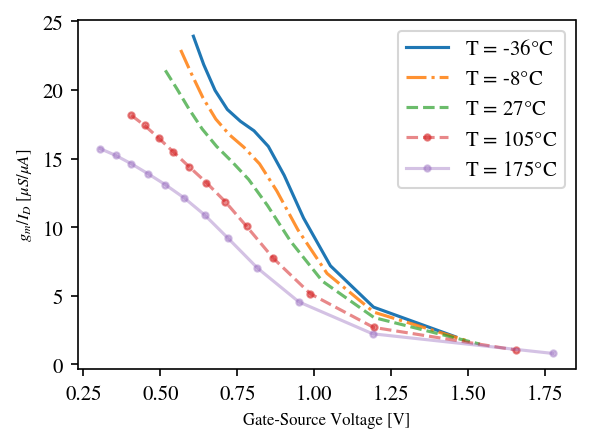
\includegraphics[width=\textwidth]{gm_nel_T}
		\resizebox {\textwidth} {!} {
			%% Creator: Matplotlib, PGF backend
%%
%% To include the figure in your LaTeX document, write
%%   \input{<filename>.pgf}
%%
%% Make sure the required packages are loaded in your preamble
%%   \usepackage{pgf}
%%
%% Figures using additional raster images can only be included by \input if
%% they are in the same directory as the main LaTeX file. For loading figures
%% from other directories you can use the `import` package
%%   \usepackage{import}
%% and then include the figures with
%%   \import{<path to file>}{<filename>.pgf}
%%
%% Matplotlib used the following preamble
%%   \usepackage{gensymb}
%%   \usepackage[utf8x]{inputenc}
%%   \usepackage[T1]{fontenc}
%%
\begingroup%
\makeatletter%
\begin{pgfpicture}%
\pgfpathrectangle{\pgfpointorigin}{\pgfqpoint{3.840000in}{2.840000in}}%
\pgfusepath{use as bounding box, clip}%
\begin{pgfscope}%
\pgfsetbuttcap%
\pgfsetmiterjoin%
\definecolor{currentfill}{rgb}{1.000000,1.000000,1.000000}%
\pgfsetfillcolor{currentfill}%
\pgfsetlinewidth{0.000000pt}%
\definecolor{currentstroke}{rgb}{1.000000,1.000000,1.000000}%
\pgfsetstrokecolor{currentstroke}%
\pgfsetdash{}{0pt}%
\pgfpathmoveto{\pgfqpoint{0.000000in}{0.000000in}}%
\pgfpathlineto{\pgfqpoint{3.840000in}{0.000000in}}%
\pgfpathlineto{\pgfqpoint{3.840000in}{2.840000in}}%
\pgfpathlineto{\pgfqpoint{0.000000in}{2.840000in}}%
\pgfpathclose%
\pgfusepath{fill}%
\end{pgfscope}%
\begin{pgfscope}%
\pgfsetbuttcap%
\pgfsetmiterjoin%
\definecolor{currentfill}{rgb}{1.000000,1.000000,1.000000}%
\pgfsetfillcolor{currentfill}%
\pgfsetlinewidth{0.000000pt}%
\definecolor{currentstroke}{rgb}{0.000000,0.000000,0.000000}%
\pgfsetstrokecolor{currentstroke}%
\pgfsetstrokeopacity{0.000000}%
\pgfsetdash{}{0pt}%
\pgfpathmoveto{\pgfqpoint{0.615275in}{0.596026in}}%
\pgfpathlineto{\pgfqpoint{3.716667in}{0.596026in}}%
\pgfpathlineto{\pgfqpoint{3.716667in}{2.716667in}}%
\pgfpathlineto{\pgfqpoint{0.615275in}{2.716667in}}%
\pgfpathclose%
\pgfusepath{fill}%
\end{pgfscope}%
\begin{pgfscope}%
\pgfsetbuttcap%
\pgfsetroundjoin%
\definecolor{currentfill}{rgb}{0.000000,0.000000,0.000000}%
\pgfsetfillcolor{currentfill}%
\pgfsetlinewidth{0.803000pt}%
\definecolor{currentstroke}{rgb}{0.000000,0.000000,0.000000}%
\pgfsetstrokecolor{currentstroke}%
\pgfsetdash{}{0pt}%
\pgfsys@defobject{currentmarker}{\pgfqpoint{0.000000in}{-0.048611in}}{\pgfqpoint{0.000000in}{0.000000in}}{%
\pgfpathmoveto{\pgfqpoint{0.000000in}{0.000000in}}%
\pgfpathlineto{\pgfqpoint{0.000000in}{-0.048611in}}%
\pgfusepath{stroke,fill}%
}%
\begin{pgfscope}%
\pgfsys@transformshift{1.130344in}{0.596026in}%
\pgfsys@useobject{currentmarker}{}%
\end{pgfscope}%
\end{pgfscope}%
\begin{pgfscope}%
\pgftext[x=1.130344in,y=0.498804in,,top]{\fontsize{14.000000}{16.800000}\selectfont \(\displaystyle 0.5\)}%
\end{pgfscope}%
\begin{pgfscope}%
\pgfsetbuttcap%
\pgfsetroundjoin%
\definecolor{currentfill}{rgb}{0.000000,0.000000,0.000000}%
\pgfsetfillcolor{currentfill}%
\pgfsetlinewidth{0.803000pt}%
\definecolor{currentstroke}{rgb}{0.000000,0.000000,0.000000}%
\pgfsetstrokecolor{currentstroke}%
\pgfsetdash{}{0pt}%
\pgfsys@defobject{currentmarker}{\pgfqpoint{0.000000in}{-0.048611in}}{\pgfqpoint{0.000000in}{0.000000in}}{%
\pgfpathmoveto{\pgfqpoint{0.000000in}{0.000000in}}%
\pgfpathlineto{\pgfqpoint{0.000000in}{-0.048611in}}%
\pgfusepath{stroke,fill}%
}%
\begin{pgfscope}%
\pgfsys@transformshift{2.090058in}{0.596026in}%
\pgfsys@useobject{currentmarker}{}%
\end{pgfscope}%
\end{pgfscope}%
\begin{pgfscope}%
\pgftext[x=2.090058in,y=0.498804in,,top]{\fontsize{14.000000}{16.800000}\selectfont \(\displaystyle 1.0\)}%
\end{pgfscope}%
\begin{pgfscope}%
\pgfsetbuttcap%
\pgfsetroundjoin%
\definecolor{currentfill}{rgb}{0.000000,0.000000,0.000000}%
\pgfsetfillcolor{currentfill}%
\pgfsetlinewidth{0.803000pt}%
\definecolor{currentstroke}{rgb}{0.000000,0.000000,0.000000}%
\pgfsetstrokecolor{currentstroke}%
\pgfsetdash{}{0pt}%
\pgfsys@defobject{currentmarker}{\pgfqpoint{0.000000in}{-0.048611in}}{\pgfqpoint{0.000000in}{0.000000in}}{%
\pgfpathmoveto{\pgfqpoint{0.000000in}{0.000000in}}%
\pgfpathlineto{\pgfqpoint{0.000000in}{-0.048611in}}%
\pgfusepath{stroke,fill}%
}%
\begin{pgfscope}%
\pgfsys@transformshift{3.049771in}{0.596026in}%
\pgfsys@useobject{currentmarker}{}%
\end{pgfscope}%
\end{pgfscope}%
\begin{pgfscope}%
\pgftext[x=3.049771in,y=0.498804in,,top]{\fontsize{14.000000}{16.800000}\selectfont \(\displaystyle 1.5\)}%
\end{pgfscope}%
\begin{pgfscope}%
\pgftext[x=2.165971in,y=0.266626in,,top]{\fontsize{12.000000}{14.400000}\selectfont Gate-Source Voltage [V]}%
\end{pgfscope}%
\begin{pgfscope}%
\pgfsetbuttcap%
\pgfsetroundjoin%
\definecolor{currentfill}{rgb}{0.000000,0.000000,0.000000}%
\pgfsetfillcolor{currentfill}%
\pgfsetlinewidth{0.803000pt}%
\definecolor{currentstroke}{rgb}{0.000000,0.000000,0.000000}%
\pgfsetstrokecolor{currentstroke}%
\pgfsetdash{}{0pt}%
\pgfsys@defobject{currentmarker}{\pgfqpoint{-0.048611in}{0.000000in}}{\pgfqpoint{0.000000in}{0.000000in}}{%
\pgfpathmoveto{\pgfqpoint{0.000000in}{0.000000in}}%
\pgfpathlineto{\pgfqpoint{-0.048611in}{0.000000in}}%
\pgfusepath{stroke,fill}%
}%
\begin{pgfscope}%
\pgfsys@transformshift{0.615275in}{0.625648in}%
\pgfsys@useobject{currentmarker}{}%
\end{pgfscope}%
\end{pgfscope}%
\begin{pgfscope}%
\pgftext[x=0.420138in,y=0.556782in,left,base]{\fontsize{14.000000}{16.800000}\selectfont \(\displaystyle 0\)}%
\end{pgfscope}%
\begin{pgfscope}%
\pgfsetbuttcap%
\pgfsetroundjoin%
\definecolor{currentfill}{rgb}{0.000000,0.000000,0.000000}%
\pgfsetfillcolor{currentfill}%
\pgfsetlinewidth{0.803000pt}%
\definecolor{currentstroke}{rgb}{0.000000,0.000000,0.000000}%
\pgfsetstrokecolor{currentstroke}%
\pgfsetdash{}{0pt}%
\pgfsys@defobject{currentmarker}{\pgfqpoint{-0.048611in}{0.000000in}}{\pgfqpoint{0.000000in}{0.000000in}}{%
\pgfpathmoveto{\pgfqpoint{0.000000in}{0.000000in}}%
\pgfpathlineto{\pgfqpoint{-0.048611in}{0.000000in}}%
\pgfusepath{stroke,fill}%
}%
\begin{pgfscope}%
\pgfsys@transformshift{0.615275in}{1.459522in}%
\pgfsys@useobject{currentmarker}{}%
\end{pgfscope}%
\end{pgfscope}%
\begin{pgfscope}%
\pgftext[x=0.322222in,y=1.390655in,left,base]{\fontsize{14.000000}{16.800000}\selectfont \(\displaystyle 10\)}%
\end{pgfscope}%
\begin{pgfscope}%
\pgfsetbuttcap%
\pgfsetroundjoin%
\definecolor{currentfill}{rgb}{0.000000,0.000000,0.000000}%
\pgfsetfillcolor{currentfill}%
\pgfsetlinewidth{0.803000pt}%
\definecolor{currentstroke}{rgb}{0.000000,0.000000,0.000000}%
\pgfsetstrokecolor{currentstroke}%
\pgfsetdash{}{0pt}%
\pgfsys@defobject{currentmarker}{\pgfqpoint{-0.048611in}{0.000000in}}{\pgfqpoint{0.000000in}{0.000000in}}{%
\pgfpathmoveto{\pgfqpoint{0.000000in}{0.000000in}}%
\pgfpathlineto{\pgfqpoint{-0.048611in}{0.000000in}}%
\pgfusepath{stroke,fill}%
}%
\begin{pgfscope}%
\pgfsys@transformshift{0.615275in}{2.293395in}%
\pgfsys@useobject{currentmarker}{}%
\end{pgfscope}%
\end{pgfscope}%
\begin{pgfscope}%
\pgftext[x=0.322222in,y=2.224529in,left,base]{\fontsize{14.000000}{16.800000}\selectfont \(\displaystyle 20\)}%
\end{pgfscope}%
\begin{pgfscope}%
\pgftext[x=0.266667in,y=1.656346in,,bottom,rotate=90.000000]{\fontsize{12.000000}{14.400000}\selectfont \(\displaystyle g_m/I_D\) [\(\displaystyle \mu S/\mu A\)]}%
\end{pgfscope}%
\begin{pgfscope}%
\pgfpathrectangle{\pgfqpoint{0.615275in}{0.596026in}}{\pgfqpoint{3.101391in}{2.120641in}} %
\pgfusepath{clip}%
\pgfsetrectcap%
\pgfsetroundjoin%
\pgfsetlinewidth{1.505625pt}%
\definecolor{currentstroke}{rgb}{0.121569,0.466667,0.705882}%
\pgfsetstrokecolor{currentstroke}%
\pgfsetdash{}{0pt}%
\pgfpathmoveto{\pgfqpoint{1.336107in}{2.620274in}}%
\pgfpathlineto{\pgfqpoint{1.400599in}{2.447472in}}%
\pgfpathlineto{\pgfqpoint{1.471234in}{2.291060in}}%
\pgfpathlineto{\pgfqpoint{1.547819in}{2.174985in}}%
\pgfpathlineto{\pgfqpoint{1.629203in}{2.103316in}}%
\pgfpathlineto{\pgfqpoint{1.713850in}{2.045497in}}%
\pgfpathlineto{\pgfqpoint{1.803103in}{1.950673in}}%
\pgfpathlineto{\pgfqpoint{1.901954in}{1.774644in}}%
\pgfpathlineto{\pgfqpoint{2.022494in}{1.515209in}}%
\pgfpathlineto{\pgfqpoint{2.189868in}{1.225120in}}%
\pgfpathlineto{\pgfqpoint{2.458588in}{0.973792in}}%
\pgfpathlineto{\pgfqpoint{2.969155in}{0.793464in}}%
\pgfusepath{stroke}%
\end{pgfscope}%
\begin{pgfscope}%
\pgfpathrectangle{\pgfqpoint{0.615275in}{0.596026in}}{\pgfqpoint{3.101391in}{2.120641in}} %
\pgfusepath{clip}%
\pgfsetbuttcap%
\pgfsetroundjoin%
\pgfsetlinewidth{1.505625pt}%
\definecolor{currentstroke}{rgb}{1.000000,0.498039,0.054902}%
\pgfsetstrokecolor{currentstroke}%
\pgfsetstrokeopacity{0.850000}%
\pgfsetdash{{9.600000pt}{2.400000pt}{1.500000pt}{2.400000pt}}{0.000000pt}%
\pgfpathmoveto{\pgfqpoint{1.257026in}{2.536887in}}%
\pgfpathlineto{\pgfqpoint{1.323822in}{2.392500in}}%
\pgfpathlineto{\pgfqpoint{1.396569in}{2.244524in}}%
\pgfpathlineto{\pgfqpoint{1.475841in}{2.116614in}}%
\pgfpathlineto{\pgfqpoint{1.561063in}{2.020984in}}%
\pgfpathlineto{\pgfqpoint{1.651660in}{1.944900in}}%
\pgfpathlineto{\pgfqpoint{1.748208in}{1.844771in}}%
\pgfpathlineto{\pgfqpoint{1.855696in}{1.680185in}}%
\pgfpathlineto{\pgfqpoint{1.986984in}{1.444073in}}%
\pgfpathlineto{\pgfqpoint{2.168754in}{1.178673in}}%
\pgfpathlineto{\pgfqpoint{2.460507in}{0.943248in}}%
\pgfpathlineto{\pgfqpoint{3.034416in}{0.771639in}}%
\pgfusepath{stroke}%
\end{pgfscope}%
\begin{pgfscope}%
\pgfpathrectangle{\pgfqpoint{0.615275in}{0.596026in}}{\pgfqpoint{3.101391in}{2.120641in}} %
\pgfusepath{clip}%
\pgfsetbuttcap%
\pgfsetroundjoin%
\pgfsetlinewidth{1.505625pt}%
\definecolor{currentstroke}{rgb}{0.172549,0.627451,0.172549}%
\pgfsetstrokecolor{currentstroke}%
\pgfsetstrokeopacity{0.700000}%
\pgfsetdash{{5.550000pt}{2.400000pt}}{0.000000pt}%
\pgfpathmoveto{\pgfqpoint{1.161439in}{2.412818in}}%
\pgfpathlineto{\pgfqpoint{1.232458in}{2.302299in}}%
\pgfpathlineto{\pgfqpoint{1.308467in}{2.178428in}}%
\pgfpathlineto{\pgfqpoint{1.391002in}{2.056575in}}%
\pgfpathlineto{\pgfqpoint{1.480256in}{1.951174in}}%
\pgfpathlineto{\pgfqpoint{1.576419in}{1.857956in}}%
\pgfpathlineto{\pgfqpoint{1.680452in}{1.749710in}}%
\pgfpathlineto{\pgfqpoint{1.797729in}{1.591532in}}%
\pgfpathlineto{\pgfqpoint{1.940918in}{1.375092in}}%
\pgfpathlineto{\pgfqpoint{2.139963in}{1.131559in}}%
\pgfpathlineto{\pgfqpoint{2.462426in}{0.909955in}}%
\pgfpathlineto{\pgfqpoint{3.120790in}{0.749220in}}%
\pgfusepath{stroke}%
\end{pgfscope}%
\begin{pgfscope}%
\pgfpathrectangle{\pgfqpoint{0.615275in}{0.596026in}}{\pgfqpoint{3.101391in}{2.120641in}} %
\pgfusepath{clip}%
\pgfsetbuttcap%
\pgfsetroundjoin%
\pgfsetlinewidth{1.505625pt}%
\definecolor{currentstroke}{rgb}{0.839216,0.152941,0.156863}%
\pgfsetstrokecolor{currentstroke}%
\pgfsetstrokeopacity{0.550000}%
\pgfsetdash{{5.550000pt}{2.400000pt}}{0.000000pt}%
\pgfpathmoveto{\pgfqpoint{0.949918in}{2.139280in}}%
\pgfpathlineto{\pgfqpoint{1.032645in}{2.077765in}}%
\pgfpathlineto{\pgfqpoint{1.119595in}{2.001782in}}%
\pgfpathlineto{\pgfqpoint{1.211728in}{1.916484in}}%
\pgfpathlineto{\pgfqpoint{1.310386in}{1.826519in}}%
\pgfpathlineto{\pgfqpoint{1.416914in}{1.730773in}}%
\pgfpathlineto{\pgfqpoint{1.534000in}{1.615456in}}%
\pgfpathlineto{\pgfqpoint{1.668167in}{1.464167in}}%
\pgfpathlineto{\pgfqpoint{1.834006in}{1.270723in}}%
\pgfpathlineto{\pgfqpoint{2.065681in}{1.054509in}}%
\pgfpathlineto{\pgfqpoint{2.458588in}{0.850685in}}%
\pgfpathlineto{\pgfqpoint{3.343444in}{0.713670in}}%
\pgfusepath{stroke}%
\end{pgfscope}%
\begin{pgfscope}%
\pgfpathrectangle{\pgfqpoint{0.615275in}{0.596026in}}{\pgfqpoint{3.101391in}{2.120641in}} %
\pgfusepath{clip}%
\pgfsetbuttcap%
\pgfsetroundjoin%
\definecolor{currentfill}{rgb}{0.839216,0.152941,0.156863}%
\pgfsetfillcolor{currentfill}%
\pgfsetfillopacity{0.550000}%
\pgfsetlinewidth{1.003750pt}%
\definecolor{currentstroke}{rgb}{0.839216,0.152941,0.156863}%
\pgfsetstrokecolor{currentstroke}%
\pgfsetstrokeopacity{0.550000}%
\pgfsetdash{}{0pt}%
\pgfsys@defobject{currentmarker}{\pgfqpoint{-0.020833in}{-0.020833in}}{\pgfqpoint{0.020833in}{0.020833in}}{%
\pgfpathmoveto{\pgfqpoint{0.000000in}{-0.020833in}}%
\pgfpathcurveto{\pgfqpoint{0.005525in}{-0.020833in}}{\pgfqpoint{0.010825in}{-0.018638in}}{\pgfqpoint{0.014731in}{-0.014731in}}%
\pgfpathcurveto{\pgfqpoint{0.018638in}{-0.010825in}}{\pgfqpoint{0.020833in}{-0.005525in}}{\pgfqpoint{0.020833in}{0.000000in}}%
\pgfpathcurveto{\pgfqpoint{0.020833in}{0.005525in}}{\pgfqpoint{0.018638in}{0.010825in}}{\pgfqpoint{0.014731in}{0.014731in}}%
\pgfpathcurveto{\pgfqpoint{0.010825in}{0.018638in}}{\pgfqpoint{0.005525in}{0.020833in}}{\pgfqpoint{0.000000in}{0.020833in}}%
\pgfpathcurveto{\pgfqpoint{-0.005525in}{0.020833in}}{\pgfqpoint{-0.010825in}{0.018638in}}{\pgfqpoint{-0.014731in}{0.014731in}}%
\pgfpathcurveto{\pgfqpoint{-0.018638in}{0.010825in}}{\pgfqpoint{-0.020833in}{0.005525in}}{\pgfqpoint{-0.020833in}{0.000000in}}%
\pgfpathcurveto{\pgfqpoint{-0.020833in}{-0.005525in}}{\pgfqpoint{-0.018638in}{-0.010825in}}{\pgfqpoint{-0.014731in}{-0.014731in}}%
\pgfpathcurveto{\pgfqpoint{-0.010825in}{-0.018638in}}{\pgfqpoint{-0.005525in}{-0.020833in}}{\pgfqpoint{0.000000in}{-0.020833in}}%
\pgfpathclose%
\pgfusepath{stroke,fill}%
}%
\begin{pgfscope}%
\pgfsys@transformshift{0.949918in}{2.139280in}%
\pgfsys@useobject{currentmarker}{}%
\end{pgfscope}%
\begin{pgfscope}%
\pgfsys@transformshift{1.032645in}{2.077765in}%
\pgfsys@useobject{currentmarker}{}%
\end{pgfscope}%
\begin{pgfscope}%
\pgfsys@transformshift{1.119595in}{2.001782in}%
\pgfsys@useobject{currentmarker}{}%
\end{pgfscope}%
\begin{pgfscope}%
\pgfsys@transformshift{1.211728in}{1.916484in}%
\pgfsys@useobject{currentmarker}{}%
\end{pgfscope}%
\begin{pgfscope}%
\pgfsys@transformshift{1.310386in}{1.826519in}%
\pgfsys@useobject{currentmarker}{}%
\end{pgfscope}%
\begin{pgfscope}%
\pgfsys@transformshift{1.416914in}{1.730773in}%
\pgfsys@useobject{currentmarker}{}%
\end{pgfscope}%
\begin{pgfscope}%
\pgfsys@transformshift{1.534000in}{1.615456in}%
\pgfsys@useobject{currentmarker}{}%
\end{pgfscope}%
\begin{pgfscope}%
\pgfsys@transformshift{1.668167in}{1.464167in}%
\pgfsys@useobject{currentmarker}{}%
\end{pgfscope}%
\begin{pgfscope}%
\pgfsys@transformshift{1.834006in}{1.270723in}%
\pgfsys@useobject{currentmarker}{}%
\end{pgfscope}%
\begin{pgfscope}%
\pgfsys@transformshift{2.065681in}{1.054509in}%
\pgfsys@useobject{currentmarker}{}%
\end{pgfscope}%
\begin{pgfscope}%
\pgfsys@transformshift{2.458588in}{0.850685in}%
\pgfsys@useobject{currentmarker}{}%
\end{pgfscope}%
\begin{pgfscope}%
\pgfsys@transformshift{3.343444in}{0.713670in}%
\pgfsys@useobject{currentmarker}{}%
\end{pgfscope}%
\end{pgfscope}%
\begin{pgfscope}%
\pgfpathrectangle{\pgfqpoint{0.615275in}{0.596026in}}{\pgfqpoint{3.101391in}{2.120641in}} %
\pgfusepath{clip}%
\pgfsetrectcap%
\pgfsetroundjoin%
\pgfsetlinewidth{1.505625pt}%
\definecolor{currentstroke}{rgb}{0.580392,0.403922,0.741176}%
\pgfsetstrokecolor{currentstroke}%
\pgfsetstrokeopacity{0.400000}%
\pgfsetdash{}{0pt}%
\pgfpathmoveto{\pgfqpoint{0.756248in}{1.936629in}}%
\pgfpathlineto{\pgfqpoint{0.851259in}{1.896202in}}%
\pgfpathlineto{\pgfqpoint{0.949918in}{1.844843in}}%
\pgfpathlineto{\pgfqpoint{1.053183in}{1.784732in}}%
\pgfpathlineto{\pgfqpoint{1.162398in}{1.717349in}}%
\pgfpathlineto{\pgfqpoint{1.279100in}{1.637362in}}%
\pgfpathlineto{\pgfqpoint{1.406741in}{1.533736in}}%
\pgfpathlineto{\pgfqpoint{1.553386in}{1.391419in}}%
\pgfpathlineto{\pgfqpoint{1.735539in}{1.211084in}}%
\pgfpathlineto{\pgfqpoint{1.993318in}{1.005727in}}%
\pgfpathlineto{\pgfqpoint{2.452829in}{0.811818in}}%
\pgfpathlineto{\pgfqpoint{3.575694in}{0.692419in}}%
\pgfusepath{stroke}%
\end{pgfscope}%
\begin{pgfscope}%
\pgfpathrectangle{\pgfqpoint{0.615275in}{0.596026in}}{\pgfqpoint{3.101391in}{2.120641in}} %
\pgfusepath{clip}%
\pgfsetbuttcap%
\pgfsetroundjoin%
\definecolor{currentfill}{rgb}{0.580392,0.403922,0.741176}%
\pgfsetfillcolor{currentfill}%
\pgfsetfillopacity{0.400000}%
\pgfsetlinewidth{1.003750pt}%
\definecolor{currentstroke}{rgb}{0.580392,0.403922,0.741176}%
\pgfsetstrokecolor{currentstroke}%
\pgfsetstrokeopacity{0.400000}%
\pgfsetdash{}{0pt}%
\pgfsys@defobject{currentmarker}{\pgfqpoint{-0.020833in}{-0.020833in}}{\pgfqpoint{0.020833in}{0.020833in}}{%
\pgfpathmoveto{\pgfqpoint{0.000000in}{-0.020833in}}%
\pgfpathcurveto{\pgfqpoint{0.005525in}{-0.020833in}}{\pgfqpoint{0.010825in}{-0.018638in}}{\pgfqpoint{0.014731in}{-0.014731in}}%
\pgfpathcurveto{\pgfqpoint{0.018638in}{-0.010825in}}{\pgfqpoint{0.020833in}{-0.005525in}}{\pgfqpoint{0.020833in}{0.000000in}}%
\pgfpathcurveto{\pgfqpoint{0.020833in}{0.005525in}}{\pgfqpoint{0.018638in}{0.010825in}}{\pgfqpoint{0.014731in}{0.014731in}}%
\pgfpathcurveto{\pgfqpoint{0.010825in}{0.018638in}}{\pgfqpoint{0.005525in}{0.020833in}}{\pgfqpoint{0.000000in}{0.020833in}}%
\pgfpathcurveto{\pgfqpoint{-0.005525in}{0.020833in}}{\pgfqpoint{-0.010825in}{0.018638in}}{\pgfqpoint{-0.014731in}{0.014731in}}%
\pgfpathcurveto{\pgfqpoint{-0.018638in}{0.010825in}}{\pgfqpoint{-0.020833in}{0.005525in}}{\pgfqpoint{-0.020833in}{0.000000in}}%
\pgfpathcurveto{\pgfqpoint{-0.020833in}{-0.005525in}}{\pgfqpoint{-0.018638in}{-0.010825in}}{\pgfqpoint{-0.014731in}{-0.014731in}}%
\pgfpathcurveto{\pgfqpoint{-0.010825in}{-0.018638in}}{\pgfqpoint{-0.005525in}{-0.020833in}}{\pgfqpoint{0.000000in}{-0.020833in}}%
\pgfpathclose%
\pgfusepath{stroke,fill}%
}%
\begin{pgfscope}%
\pgfsys@transformshift{0.756248in}{1.936629in}%
\pgfsys@useobject{currentmarker}{}%
\end{pgfscope}%
\begin{pgfscope}%
\pgfsys@transformshift{0.851259in}{1.896202in}%
\pgfsys@useobject{currentmarker}{}%
\end{pgfscope}%
\begin{pgfscope}%
\pgfsys@transformshift{0.949918in}{1.844843in}%
\pgfsys@useobject{currentmarker}{}%
\end{pgfscope}%
\begin{pgfscope}%
\pgfsys@transformshift{1.053183in}{1.784732in}%
\pgfsys@useobject{currentmarker}{}%
\end{pgfscope}%
\begin{pgfscope}%
\pgfsys@transformshift{1.162398in}{1.717349in}%
\pgfsys@useobject{currentmarker}{}%
\end{pgfscope}%
\begin{pgfscope}%
\pgfsys@transformshift{1.279100in}{1.637362in}%
\pgfsys@useobject{currentmarker}{}%
\end{pgfscope}%
\begin{pgfscope}%
\pgfsys@transformshift{1.406741in}{1.533736in}%
\pgfsys@useobject{currentmarker}{}%
\end{pgfscope}%
\begin{pgfscope}%
\pgfsys@transformshift{1.553386in}{1.391419in}%
\pgfsys@useobject{currentmarker}{}%
\end{pgfscope}%
\begin{pgfscope}%
\pgfsys@transformshift{1.735539in}{1.211084in}%
\pgfsys@useobject{currentmarker}{}%
\end{pgfscope}%
\begin{pgfscope}%
\pgfsys@transformshift{1.993318in}{1.005727in}%
\pgfsys@useobject{currentmarker}{}%
\end{pgfscope}%
\begin{pgfscope}%
\pgfsys@transformshift{2.452829in}{0.811818in}%
\pgfsys@useobject{currentmarker}{}%
\end{pgfscope}%
\begin{pgfscope}%
\pgfsys@transformshift{3.575694in}{0.692419in}%
\pgfsys@useobject{currentmarker}{}%
\end{pgfscope}%
\end{pgfscope}%
\begin{pgfscope}%
\pgfsetrectcap%
\pgfsetmiterjoin%
\pgfsetlinewidth{0.803000pt}%
\definecolor{currentstroke}{rgb}{0.000000,0.000000,0.000000}%
\pgfsetstrokecolor{currentstroke}%
\pgfsetdash{}{0pt}%
\pgfpathmoveto{\pgfqpoint{0.615275in}{0.596026in}}%
\pgfpathlineto{\pgfqpoint{0.615275in}{2.716667in}}%
\pgfusepath{stroke}%
\end{pgfscope}%
\begin{pgfscope}%
\pgfsetrectcap%
\pgfsetmiterjoin%
\pgfsetlinewidth{0.803000pt}%
\definecolor{currentstroke}{rgb}{0.000000,0.000000,0.000000}%
\pgfsetstrokecolor{currentstroke}%
\pgfsetdash{}{0pt}%
\pgfpathmoveto{\pgfqpoint{3.716667in}{0.596026in}}%
\pgfpathlineto{\pgfqpoint{3.716667in}{2.716667in}}%
\pgfusepath{stroke}%
\end{pgfscope}%
\begin{pgfscope}%
\pgfsetrectcap%
\pgfsetmiterjoin%
\pgfsetlinewidth{0.803000pt}%
\definecolor{currentstroke}{rgb}{0.000000,0.000000,0.000000}%
\pgfsetstrokecolor{currentstroke}%
\pgfsetdash{}{0pt}%
\pgfpathmoveto{\pgfqpoint{0.615275in}{0.596026in}}%
\pgfpathlineto{\pgfqpoint{3.716667in}{0.596026in}}%
\pgfusepath{stroke}%
\end{pgfscope}%
\begin{pgfscope}%
\pgfsetrectcap%
\pgfsetmiterjoin%
\pgfsetlinewidth{0.803000pt}%
\definecolor{currentstroke}{rgb}{0.000000,0.000000,0.000000}%
\pgfsetstrokecolor{currentstroke}%
\pgfsetdash{}{0pt}%
\pgfpathmoveto{\pgfqpoint{0.615275in}{2.716667in}}%
\pgfpathlineto{\pgfqpoint{3.716667in}{2.716667in}}%
\pgfusepath{stroke}%
\end{pgfscope}%
\begin{pgfscope}%
\pgfsetbuttcap%
\pgfsetmiterjoin%
\definecolor{currentfill}{rgb}{1.000000,1.000000,1.000000}%
\pgfsetfillcolor{currentfill}%
\pgfsetfillopacity{0.800000}%
\pgfsetlinewidth{1.003750pt}%
\definecolor{currentstroke}{rgb}{0.800000,0.800000,0.800000}%
\pgfsetstrokecolor{currentstroke}%
\pgfsetstrokeopacity{0.800000}%
\pgfsetdash{}{0pt}%
\pgfpathmoveto{\pgfqpoint{2.501731in}{1.637224in}}%
\pgfpathlineto{\pgfqpoint{3.619444in}{1.637224in}}%
\pgfpathquadraticcurveto{\pgfqpoint{3.647222in}{1.637224in}}{\pgfqpoint{3.647222in}{1.665002in}}%
\pgfpathlineto{\pgfqpoint{3.647222in}{2.619444in}}%
\pgfpathquadraticcurveto{\pgfqpoint{3.647222in}{2.647222in}}{\pgfqpoint{3.619444in}{2.647222in}}%
\pgfpathlineto{\pgfqpoint{2.501731in}{2.647222in}}%
\pgfpathquadraticcurveto{\pgfqpoint{2.473953in}{2.647222in}}{\pgfqpoint{2.473953in}{2.619444in}}%
\pgfpathlineto{\pgfqpoint{2.473953in}{1.665002in}}%
\pgfpathquadraticcurveto{\pgfqpoint{2.473953in}{1.637224in}}{\pgfqpoint{2.501731in}{1.637224in}}%
\pgfpathclose%
\pgfusepath{stroke,fill}%
\end{pgfscope}%
\begin{pgfscope}%
\pgfsetrectcap%
\pgfsetroundjoin%
\pgfsetlinewidth{1.505625pt}%
\definecolor{currentstroke}{rgb}{0.121569,0.466667,0.705882}%
\pgfsetstrokecolor{currentstroke}%
\pgfsetdash{}{0pt}%
\pgfpathmoveto{\pgfqpoint{2.529508in}{2.543056in}}%
\pgfpathlineto{\pgfqpoint{2.807286in}{2.543056in}}%
\pgfusepath{stroke}%
\end{pgfscope}%
\begin{pgfscope}%
\pgftext[x=2.918397in,y=2.494444in,left,base]{\fontsize{10.000000}{12.000000}\selectfont T = -36\(\displaystyle \degree\)C}%
\end{pgfscope}%
\begin{pgfscope}%
\pgfsetbuttcap%
\pgfsetroundjoin%
\pgfsetlinewidth{1.505625pt}%
\definecolor{currentstroke}{rgb}{1.000000,0.498039,0.054902}%
\pgfsetstrokecolor{currentstroke}%
\pgfsetstrokeopacity{0.850000}%
\pgfsetdash{{9.600000pt}{2.400000pt}{1.500000pt}{2.400000pt}}{0.000000pt}%
\pgfpathmoveto{\pgfqpoint{2.529508in}{2.349389in}}%
\pgfpathlineto{\pgfqpoint{2.807286in}{2.349389in}}%
\pgfusepath{stroke}%
\end{pgfscope}%
\begin{pgfscope}%
\pgftext[x=2.918397in,y=2.300778in,left,base]{\fontsize{10.000000}{12.000000}\selectfont T = -8\(\displaystyle \degree\)C}%
\end{pgfscope}%
\begin{pgfscope}%
\pgfsetbuttcap%
\pgfsetroundjoin%
\pgfsetlinewidth{1.505625pt}%
\definecolor{currentstroke}{rgb}{0.172549,0.627451,0.172549}%
\pgfsetstrokecolor{currentstroke}%
\pgfsetstrokeopacity{0.700000}%
\pgfsetdash{{5.550000pt}{2.400000pt}}{0.000000pt}%
\pgfpathmoveto{\pgfqpoint{2.529508in}{2.155723in}}%
\pgfpathlineto{\pgfqpoint{2.807286in}{2.155723in}}%
\pgfusepath{stroke}%
\end{pgfscope}%
\begin{pgfscope}%
\pgftext[x=2.918397in,y=2.107112in,left,base]{\fontsize{10.000000}{12.000000}\selectfont T = 27\(\displaystyle \degree\)C}%
\end{pgfscope}%
\begin{pgfscope}%
\pgfsetbuttcap%
\pgfsetroundjoin%
\pgfsetlinewidth{1.505625pt}%
\definecolor{currentstroke}{rgb}{0.839216,0.152941,0.156863}%
\pgfsetstrokecolor{currentstroke}%
\pgfsetstrokeopacity{0.550000}%
\pgfsetdash{{5.550000pt}{2.400000pt}}{0.000000pt}%
\pgfpathmoveto{\pgfqpoint{2.529508in}{1.962057in}}%
\pgfpathlineto{\pgfqpoint{2.807286in}{1.962057in}}%
\pgfusepath{stroke}%
\end{pgfscope}%
\begin{pgfscope}%
\pgfsetbuttcap%
\pgfsetroundjoin%
\definecolor{currentfill}{rgb}{0.839216,0.152941,0.156863}%
\pgfsetfillcolor{currentfill}%
\pgfsetfillopacity{0.550000}%
\pgfsetlinewidth{1.003750pt}%
\definecolor{currentstroke}{rgb}{0.839216,0.152941,0.156863}%
\pgfsetstrokecolor{currentstroke}%
\pgfsetstrokeopacity{0.550000}%
\pgfsetdash{}{0pt}%
\pgfsys@defobject{currentmarker}{\pgfqpoint{-0.020833in}{-0.020833in}}{\pgfqpoint{0.020833in}{0.020833in}}{%
\pgfpathmoveto{\pgfqpoint{0.000000in}{-0.020833in}}%
\pgfpathcurveto{\pgfqpoint{0.005525in}{-0.020833in}}{\pgfqpoint{0.010825in}{-0.018638in}}{\pgfqpoint{0.014731in}{-0.014731in}}%
\pgfpathcurveto{\pgfqpoint{0.018638in}{-0.010825in}}{\pgfqpoint{0.020833in}{-0.005525in}}{\pgfqpoint{0.020833in}{0.000000in}}%
\pgfpathcurveto{\pgfqpoint{0.020833in}{0.005525in}}{\pgfqpoint{0.018638in}{0.010825in}}{\pgfqpoint{0.014731in}{0.014731in}}%
\pgfpathcurveto{\pgfqpoint{0.010825in}{0.018638in}}{\pgfqpoint{0.005525in}{0.020833in}}{\pgfqpoint{0.000000in}{0.020833in}}%
\pgfpathcurveto{\pgfqpoint{-0.005525in}{0.020833in}}{\pgfqpoint{-0.010825in}{0.018638in}}{\pgfqpoint{-0.014731in}{0.014731in}}%
\pgfpathcurveto{\pgfqpoint{-0.018638in}{0.010825in}}{\pgfqpoint{-0.020833in}{0.005525in}}{\pgfqpoint{-0.020833in}{0.000000in}}%
\pgfpathcurveto{\pgfqpoint{-0.020833in}{-0.005525in}}{\pgfqpoint{-0.018638in}{-0.010825in}}{\pgfqpoint{-0.014731in}{-0.014731in}}%
\pgfpathcurveto{\pgfqpoint{-0.010825in}{-0.018638in}}{\pgfqpoint{-0.005525in}{-0.020833in}}{\pgfqpoint{0.000000in}{-0.020833in}}%
\pgfpathclose%
\pgfusepath{stroke,fill}%
}%
\begin{pgfscope}%
\pgfsys@transformshift{2.668397in}{1.962057in}%
\pgfsys@useobject{currentmarker}{}%
\end{pgfscope}%
\end{pgfscope}%
\begin{pgfscope}%
\pgftext[x=2.918397in,y=1.913446in,left,base]{\fontsize{10.000000}{12.000000}\selectfont T = 105\(\displaystyle \degree\)C}%
\end{pgfscope}%
\begin{pgfscope}%
\pgfsetrectcap%
\pgfsetroundjoin%
\pgfsetlinewidth{1.505625pt}%
\definecolor{currentstroke}{rgb}{0.580392,0.403922,0.741176}%
\pgfsetstrokecolor{currentstroke}%
\pgfsetstrokeopacity{0.400000}%
\pgfsetdash{}{0pt}%
\pgfpathmoveto{\pgfqpoint{2.529508in}{1.768391in}}%
\pgfpathlineto{\pgfqpoint{2.807286in}{1.768391in}}%
\pgfusepath{stroke}%
\end{pgfscope}%
\begin{pgfscope}%
\pgfsetbuttcap%
\pgfsetroundjoin%
\definecolor{currentfill}{rgb}{0.580392,0.403922,0.741176}%
\pgfsetfillcolor{currentfill}%
\pgfsetfillopacity{0.400000}%
\pgfsetlinewidth{1.003750pt}%
\definecolor{currentstroke}{rgb}{0.580392,0.403922,0.741176}%
\pgfsetstrokecolor{currentstroke}%
\pgfsetstrokeopacity{0.400000}%
\pgfsetdash{}{0pt}%
\pgfsys@defobject{currentmarker}{\pgfqpoint{-0.020833in}{-0.020833in}}{\pgfqpoint{0.020833in}{0.020833in}}{%
\pgfpathmoveto{\pgfqpoint{0.000000in}{-0.020833in}}%
\pgfpathcurveto{\pgfqpoint{0.005525in}{-0.020833in}}{\pgfqpoint{0.010825in}{-0.018638in}}{\pgfqpoint{0.014731in}{-0.014731in}}%
\pgfpathcurveto{\pgfqpoint{0.018638in}{-0.010825in}}{\pgfqpoint{0.020833in}{-0.005525in}}{\pgfqpoint{0.020833in}{0.000000in}}%
\pgfpathcurveto{\pgfqpoint{0.020833in}{0.005525in}}{\pgfqpoint{0.018638in}{0.010825in}}{\pgfqpoint{0.014731in}{0.014731in}}%
\pgfpathcurveto{\pgfqpoint{0.010825in}{0.018638in}}{\pgfqpoint{0.005525in}{0.020833in}}{\pgfqpoint{0.000000in}{0.020833in}}%
\pgfpathcurveto{\pgfqpoint{-0.005525in}{0.020833in}}{\pgfqpoint{-0.010825in}{0.018638in}}{\pgfqpoint{-0.014731in}{0.014731in}}%
\pgfpathcurveto{\pgfqpoint{-0.018638in}{0.010825in}}{\pgfqpoint{-0.020833in}{0.005525in}}{\pgfqpoint{-0.020833in}{0.000000in}}%
\pgfpathcurveto{\pgfqpoint{-0.020833in}{-0.005525in}}{\pgfqpoint{-0.018638in}{-0.010825in}}{\pgfqpoint{-0.014731in}{-0.014731in}}%
\pgfpathcurveto{\pgfqpoint{-0.010825in}{-0.018638in}}{\pgfqpoint{-0.005525in}{-0.020833in}}{\pgfqpoint{0.000000in}{-0.020833in}}%
\pgfpathclose%
\pgfusepath{stroke,fill}%
}%
\begin{pgfscope}%
\pgfsys@transformshift{2.668397in}{1.768391in}%
\pgfsys@useobject{currentmarker}{}%
\end{pgfscope}%
\end{pgfscope}%
\begin{pgfscope}%
\pgftext[x=2.918397in,y=1.719779in,left,base]{\fontsize{10.000000}{12.000000}\selectfont T = 175\(\displaystyle \degree\)C}%
\end{pgfscope}%
\end{pgfpicture}%
\makeatother%
\endgroup%

		}
		\subcaption{Temperature effect for \(L = L_{\min}\)}
		\label{fig:gm_nel_T}
	\end{subfigure}
	\begin{subfigure}[b]{0.48\textwidth}
		%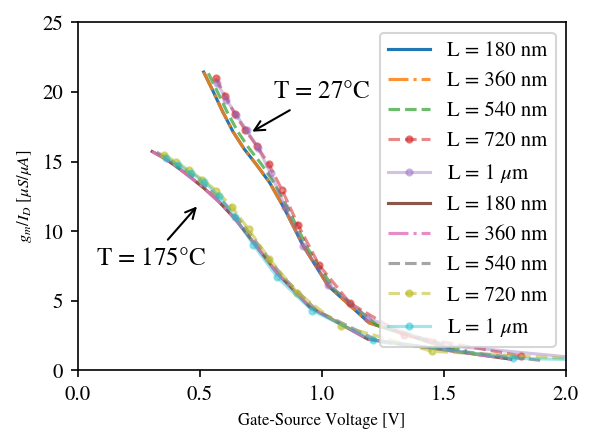
\includegraphics[width=\textwidth]{gm_nel_L}
		\resizebox {\textwidth} {!} {
			%% Creator: Matplotlib, PGF backend
%%
%% To include the figure in your LaTeX document, write
%%   \input{<filename>.pgf}
%%
%% Make sure the required packages are loaded in your preamble
%%   \usepackage{pgf}
%%
%% Figures using additional raster images can only be included by \input if
%% they are in the same directory as the main LaTeX file. For loading figures
%% from other directories you can use the `import` package
%%   \usepackage{import}
%% and then include the figures with
%%   \import{<path to file>}{<filename>.pgf}
%%
%% Matplotlib used the following preamble
%%   \usepackage{gensymb}
%%   \usepackage[utf8x]{inputenc}
%%   \usepackage[T1]{fontenc}
%%
\begingroup%
\makeatletter%
\begin{pgfpicture}%
\pgfpathrectangle{\pgfpointorigin}{\pgfqpoint{3.840000in}{2.840000in}}%
\pgfusepath{use as bounding box, clip}%
\begin{pgfscope}%
\pgfsetbuttcap%
\pgfsetmiterjoin%
\definecolor{currentfill}{rgb}{1.000000,1.000000,1.000000}%
\pgfsetfillcolor{currentfill}%
\pgfsetlinewidth{0.000000pt}%
\definecolor{currentstroke}{rgb}{1.000000,1.000000,1.000000}%
\pgfsetstrokecolor{currentstroke}%
\pgfsetdash{}{0pt}%
\pgfpathmoveto{\pgfqpoint{0.000000in}{0.000000in}}%
\pgfpathlineto{\pgfqpoint{3.840000in}{0.000000in}}%
\pgfpathlineto{\pgfqpoint{3.840000in}{2.840000in}}%
\pgfpathlineto{\pgfqpoint{0.000000in}{2.840000in}}%
\pgfpathclose%
\pgfusepath{fill}%
\end{pgfscope}%
\begin{pgfscope}%
\pgfsetbuttcap%
\pgfsetmiterjoin%
\definecolor{currentfill}{rgb}{1.000000,1.000000,1.000000}%
\pgfsetfillcolor{currentfill}%
\pgfsetlinewidth{0.000000pt}%
\definecolor{currentstroke}{rgb}{0.000000,0.000000,0.000000}%
\pgfsetstrokecolor{currentstroke}%
\pgfsetstrokeopacity{0.000000}%
\pgfsetdash{}{0pt}%
\pgfpathmoveto{\pgfqpoint{0.615275in}{0.596026in}}%
\pgfpathlineto{\pgfqpoint{3.614886in}{0.596026in}}%
\pgfpathlineto{\pgfqpoint{3.614886in}{2.671134in}}%
\pgfpathlineto{\pgfqpoint{0.615275in}{2.671134in}}%
\pgfpathclose%
\pgfusepath{fill}%
\end{pgfscope}%
\begin{pgfscope}%
\pgfsetbuttcap%
\pgfsetroundjoin%
\definecolor{currentfill}{rgb}{0.000000,0.000000,0.000000}%
\pgfsetfillcolor{currentfill}%
\pgfsetlinewidth{0.803000pt}%
\definecolor{currentstroke}{rgb}{0.000000,0.000000,0.000000}%
\pgfsetstrokecolor{currentstroke}%
\pgfsetdash{}{0pt}%
\pgfsys@defobject{currentmarker}{\pgfqpoint{0.000000in}{-0.048611in}}{\pgfqpoint{0.000000in}{0.000000in}}{%
\pgfpathmoveto{\pgfqpoint{0.000000in}{0.000000in}}%
\pgfpathlineto{\pgfqpoint{0.000000in}{-0.048611in}}%
\pgfusepath{stroke,fill}%
}%
\begin{pgfscope}%
\pgfsys@transformshift{0.615275in}{0.596026in}%
\pgfsys@useobject{currentmarker}{}%
\end{pgfscope}%
\end{pgfscope}%
\begin{pgfscope}%
\pgftext[x=0.615275in,y=0.498804in,,top]{\fontsize{14.000000}{16.800000}\selectfont \(\displaystyle 0.0\)}%
\end{pgfscope}%
\begin{pgfscope}%
\pgfsetbuttcap%
\pgfsetroundjoin%
\definecolor{currentfill}{rgb}{0.000000,0.000000,0.000000}%
\pgfsetfillcolor{currentfill}%
\pgfsetlinewidth{0.803000pt}%
\definecolor{currentstroke}{rgb}{0.000000,0.000000,0.000000}%
\pgfsetstrokecolor{currentstroke}%
\pgfsetdash{}{0pt}%
\pgfsys@defobject{currentmarker}{\pgfqpoint{0.000000in}{-0.048611in}}{\pgfqpoint{0.000000in}{0.000000in}}{%
\pgfpathmoveto{\pgfqpoint{0.000000in}{0.000000in}}%
\pgfpathlineto{\pgfqpoint{0.000000in}{-0.048611in}}%
\pgfusepath{stroke,fill}%
}%
\begin{pgfscope}%
\pgfsys@transformshift{1.365178in}{0.596026in}%
\pgfsys@useobject{currentmarker}{}%
\end{pgfscope}%
\end{pgfscope}%
\begin{pgfscope}%
\pgftext[x=1.365178in,y=0.498804in,,top]{\fontsize{14.000000}{16.800000}\selectfont \(\displaystyle 0.5\)}%
\end{pgfscope}%
\begin{pgfscope}%
\pgfsetbuttcap%
\pgfsetroundjoin%
\definecolor{currentfill}{rgb}{0.000000,0.000000,0.000000}%
\pgfsetfillcolor{currentfill}%
\pgfsetlinewidth{0.803000pt}%
\definecolor{currentstroke}{rgb}{0.000000,0.000000,0.000000}%
\pgfsetstrokecolor{currentstroke}%
\pgfsetdash{}{0pt}%
\pgfsys@defobject{currentmarker}{\pgfqpoint{0.000000in}{-0.048611in}}{\pgfqpoint{0.000000in}{0.000000in}}{%
\pgfpathmoveto{\pgfqpoint{0.000000in}{0.000000in}}%
\pgfpathlineto{\pgfqpoint{0.000000in}{-0.048611in}}%
\pgfusepath{stroke,fill}%
}%
\begin{pgfscope}%
\pgfsys@transformshift{2.115081in}{0.596026in}%
\pgfsys@useobject{currentmarker}{}%
\end{pgfscope}%
\end{pgfscope}%
\begin{pgfscope}%
\pgftext[x=2.115081in,y=0.498804in,,top]{\fontsize{14.000000}{16.800000}\selectfont \(\displaystyle 1.0\)}%
\end{pgfscope}%
\begin{pgfscope}%
\pgfsetbuttcap%
\pgfsetroundjoin%
\definecolor{currentfill}{rgb}{0.000000,0.000000,0.000000}%
\pgfsetfillcolor{currentfill}%
\pgfsetlinewidth{0.803000pt}%
\definecolor{currentstroke}{rgb}{0.000000,0.000000,0.000000}%
\pgfsetstrokecolor{currentstroke}%
\pgfsetdash{}{0pt}%
\pgfsys@defobject{currentmarker}{\pgfqpoint{0.000000in}{-0.048611in}}{\pgfqpoint{0.000000in}{0.000000in}}{%
\pgfpathmoveto{\pgfqpoint{0.000000in}{0.000000in}}%
\pgfpathlineto{\pgfqpoint{0.000000in}{-0.048611in}}%
\pgfusepath{stroke,fill}%
}%
\begin{pgfscope}%
\pgfsys@transformshift{2.864983in}{0.596026in}%
\pgfsys@useobject{currentmarker}{}%
\end{pgfscope}%
\end{pgfscope}%
\begin{pgfscope}%
\pgftext[x=2.864983in,y=0.498804in,,top]{\fontsize{14.000000}{16.800000}\selectfont \(\displaystyle 1.5\)}%
\end{pgfscope}%
\begin{pgfscope}%
\pgfsetbuttcap%
\pgfsetroundjoin%
\definecolor{currentfill}{rgb}{0.000000,0.000000,0.000000}%
\pgfsetfillcolor{currentfill}%
\pgfsetlinewidth{0.803000pt}%
\definecolor{currentstroke}{rgb}{0.000000,0.000000,0.000000}%
\pgfsetstrokecolor{currentstroke}%
\pgfsetdash{}{0pt}%
\pgfsys@defobject{currentmarker}{\pgfqpoint{0.000000in}{-0.048611in}}{\pgfqpoint{0.000000in}{0.000000in}}{%
\pgfpathmoveto{\pgfqpoint{0.000000in}{0.000000in}}%
\pgfpathlineto{\pgfqpoint{0.000000in}{-0.048611in}}%
\pgfusepath{stroke,fill}%
}%
\begin{pgfscope}%
\pgfsys@transformshift{3.614886in}{0.596026in}%
\pgfsys@useobject{currentmarker}{}%
\end{pgfscope}%
\end{pgfscope}%
\begin{pgfscope}%
\pgftext[x=3.614886in,y=0.498804in,,top]{\fontsize{14.000000}{16.800000}\selectfont \(\displaystyle 2.0\)}%
\end{pgfscope}%
\begin{pgfscope}%
\pgftext[x=2.115081in,y=0.266626in,,top]{\fontsize{12.000000}{14.400000}\selectfont Gate-Source Voltage [V]}%
\end{pgfscope}%
\begin{pgfscope}%
\pgfsetbuttcap%
\pgfsetroundjoin%
\definecolor{currentfill}{rgb}{0.000000,0.000000,0.000000}%
\pgfsetfillcolor{currentfill}%
\pgfsetlinewidth{0.803000pt}%
\definecolor{currentstroke}{rgb}{0.000000,0.000000,0.000000}%
\pgfsetstrokecolor{currentstroke}%
\pgfsetdash{}{0pt}%
\pgfsys@defobject{currentmarker}{\pgfqpoint{-0.048611in}{0.000000in}}{\pgfqpoint{0.000000in}{0.000000in}}{%
\pgfpathmoveto{\pgfqpoint{0.000000in}{0.000000in}}%
\pgfpathlineto{\pgfqpoint{-0.048611in}{0.000000in}}%
\pgfusepath{stroke,fill}%
}%
\begin{pgfscope}%
\pgfsys@transformshift{0.615275in}{0.596026in}%
\pgfsys@useobject{currentmarker}{}%
\end{pgfscope}%
\end{pgfscope}%
\begin{pgfscope}%
\pgftext[x=0.420138in,y=0.527160in,left,base]{\fontsize{14.000000}{16.800000}\selectfont \(\displaystyle 0\)}%
\end{pgfscope}%
\begin{pgfscope}%
\pgfsetbuttcap%
\pgfsetroundjoin%
\definecolor{currentfill}{rgb}{0.000000,0.000000,0.000000}%
\pgfsetfillcolor{currentfill}%
\pgfsetlinewidth{0.803000pt}%
\definecolor{currentstroke}{rgb}{0.000000,0.000000,0.000000}%
\pgfsetstrokecolor{currentstroke}%
\pgfsetdash{}{0pt}%
\pgfsys@defobject{currentmarker}{\pgfqpoint{-0.048611in}{0.000000in}}{\pgfqpoint{0.000000in}{0.000000in}}{%
\pgfpathmoveto{\pgfqpoint{0.000000in}{0.000000in}}%
\pgfpathlineto{\pgfqpoint{-0.048611in}{0.000000in}}%
\pgfusepath{stroke,fill}%
}%
\begin{pgfscope}%
\pgfsys@transformshift{0.615275in}{1.011048in}%
\pgfsys@useobject{currentmarker}{}%
\end{pgfscope}%
\end{pgfscope}%
\begin{pgfscope}%
\pgftext[x=0.420138in,y=0.942181in,left,base]{\fontsize{14.000000}{16.800000}\selectfont \(\displaystyle 5\)}%
\end{pgfscope}%
\begin{pgfscope}%
\pgfsetbuttcap%
\pgfsetroundjoin%
\definecolor{currentfill}{rgb}{0.000000,0.000000,0.000000}%
\pgfsetfillcolor{currentfill}%
\pgfsetlinewidth{0.803000pt}%
\definecolor{currentstroke}{rgb}{0.000000,0.000000,0.000000}%
\pgfsetstrokecolor{currentstroke}%
\pgfsetdash{}{0pt}%
\pgfsys@defobject{currentmarker}{\pgfqpoint{-0.048611in}{0.000000in}}{\pgfqpoint{0.000000in}{0.000000in}}{%
\pgfpathmoveto{\pgfqpoint{0.000000in}{0.000000in}}%
\pgfpathlineto{\pgfqpoint{-0.048611in}{0.000000in}}%
\pgfusepath{stroke,fill}%
}%
\begin{pgfscope}%
\pgfsys@transformshift{0.615275in}{1.426069in}%
\pgfsys@useobject{currentmarker}{}%
\end{pgfscope}%
\end{pgfscope}%
\begin{pgfscope}%
\pgftext[x=0.322222in,y=1.357203in,left,base]{\fontsize{14.000000}{16.800000}\selectfont \(\displaystyle 10\)}%
\end{pgfscope}%
\begin{pgfscope}%
\pgfsetbuttcap%
\pgfsetroundjoin%
\definecolor{currentfill}{rgb}{0.000000,0.000000,0.000000}%
\pgfsetfillcolor{currentfill}%
\pgfsetlinewidth{0.803000pt}%
\definecolor{currentstroke}{rgb}{0.000000,0.000000,0.000000}%
\pgfsetstrokecolor{currentstroke}%
\pgfsetdash{}{0pt}%
\pgfsys@defobject{currentmarker}{\pgfqpoint{-0.048611in}{0.000000in}}{\pgfqpoint{0.000000in}{0.000000in}}{%
\pgfpathmoveto{\pgfqpoint{0.000000in}{0.000000in}}%
\pgfpathlineto{\pgfqpoint{-0.048611in}{0.000000in}}%
\pgfusepath{stroke,fill}%
}%
\begin{pgfscope}%
\pgfsys@transformshift{0.615275in}{1.841091in}%
\pgfsys@useobject{currentmarker}{}%
\end{pgfscope}%
\end{pgfscope}%
\begin{pgfscope}%
\pgftext[x=0.322222in,y=1.772225in,left,base]{\fontsize{14.000000}{16.800000}\selectfont \(\displaystyle 15\)}%
\end{pgfscope}%
\begin{pgfscope}%
\pgfsetbuttcap%
\pgfsetroundjoin%
\definecolor{currentfill}{rgb}{0.000000,0.000000,0.000000}%
\pgfsetfillcolor{currentfill}%
\pgfsetlinewidth{0.803000pt}%
\definecolor{currentstroke}{rgb}{0.000000,0.000000,0.000000}%
\pgfsetstrokecolor{currentstroke}%
\pgfsetdash{}{0pt}%
\pgfsys@defobject{currentmarker}{\pgfqpoint{-0.048611in}{0.000000in}}{\pgfqpoint{0.000000in}{0.000000in}}{%
\pgfpathmoveto{\pgfqpoint{0.000000in}{0.000000in}}%
\pgfpathlineto{\pgfqpoint{-0.048611in}{0.000000in}}%
\pgfusepath{stroke,fill}%
}%
\begin{pgfscope}%
\pgfsys@transformshift{0.615275in}{2.256112in}%
\pgfsys@useobject{currentmarker}{}%
\end{pgfscope}%
\end{pgfscope}%
\begin{pgfscope}%
\pgftext[x=0.322222in,y=2.187246in,left,base]{\fontsize{14.000000}{16.800000}\selectfont \(\displaystyle 20\)}%
\end{pgfscope}%
\begin{pgfscope}%
\pgfsetbuttcap%
\pgfsetroundjoin%
\definecolor{currentfill}{rgb}{0.000000,0.000000,0.000000}%
\pgfsetfillcolor{currentfill}%
\pgfsetlinewidth{0.803000pt}%
\definecolor{currentstroke}{rgb}{0.000000,0.000000,0.000000}%
\pgfsetstrokecolor{currentstroke}%
\pgfsetdash{}{0pt}%
\pgfsys@defobject{currentmarker}{\pgfqpoint{-0.048611in}{0.000000in}}{\pgfqpoint{0.000000in}{0.000000in}}{%
\pgfpathmoveto{\pgfqpoint{0.000000in}{0.000000in}}%
\pgfpathlineto{\pgfqpoint{-0.048611in}{0.000000in}}%
\pgfusepath{stroke,fill}%
}%
\begin{pgfscope}%
\pgfsys@transformshift{0.615275in}{2.671134in}%
\pgfsys@useobject{currentmarker}{}%
\end{pgfscope}%
\end{pgfscope}%
\begin{pgfscope}%
\pgftext[x=0.322222in,y=2.602268in,left,base]{\fontsize{14.000000}{16.800000}\selectfont \(\displaystyle 25\)}%
\end{pgfscope}%
\begin{pgfscope}%
\pgftext[x=0.266667in,y=1.633580in,,bottom,rotate=90.000000]{\fontsize{12.000000}{14.400000}\selectfont \(\displaystyle g_m/I_D\) [\(\displaystyle \mu S/\mu A\)]}%
\end{pgfscope}%
\begin{pgfscope}%
\pgfpathrectangle{\pgfqpoint{0.615275in}{0.596026in}}{\pgfqpoint{2.999611in}{2.075108in}} %
\pgfusepath{clip}%
\pgfsetrectcap%
\pgfsetroundjoin%
\pgfsetlinewidth{1.505625pt}%
\definecolor{currentstroke}{rgb}{0.121569,0.466667,0.705882}%
\pgfsetstrokecolor{currentstroke}%
\pgfsetdash{}{0pt}%
\pgfpathmoveto{\pgfqpoint{1.389475in}{2.374986in}}%
\pgfpathlineto{\pgfqpoint{1.444968in}{2.264975in}}%
\pgfpathlineto{\pgfqpoint{1.504360in}{2.141673in}}%
\pgfpathlineto{\pgfqpoint{1.568852in}{2.020380in}}%
\pgfpathlineto{\pgfqpoint{1.638592in}{1.915463in}}%
\pgfpathlineto{\pgfqpoint{1.713733in}{1.822673in}}%
\pgfpathlineto{\pgfqpoint{1.795022in}{1.714924in}}%
\pgfpathlineto{\pgfqpoint{1.886660in}{1.557473in}}%
\pgfpathlineto{\pgfqpoint{1.998546in}{1.342028in}}%
\pgfpathlineto{\pgfqpoint{2.154076in}{1.099613in}}%
\pgfpathlineto{\pgfqpoint{2.406043in}{0.879027in}}%
\pgfpathlineto{\pgfqpoint{2.920476in}{0.719030in}}%
\pgfusepath{stroke}%
\end{pgfscope}%
\begin{pgfscope}%
\pgfpathrectangle{\pgfqpoint{0.615275in}{0.596026in}}{\pgfqpoint{2.999611in}{2.075108in}} %
\pgfusepath{clip}%
\pgfsetbuttcap%
\pgfsetroundjoin%
\pgfsetlinewidth{1.505625pt}%
\definecolor{currentstroke}{rgb}{1.000000,0.498039,0.054902}%
\pgfsetstrokecolor{currentstroke}%
\pgfsetstrokeopacity{0.850000}%
\pgfsetdash{{9.600000pt}{2.400000pt}{1.500000pt}{2.400000pt}}{0.000000pt}%
\pgfpathmoveto{\pgfqpoint{1.389475in}{2.374986in}}%
\pgfpathlineto{\pgfqpoint{1.444968in}{2.264975in}}%
\pgfpathlineto{\pgfqpoint{1.504360in}{2.141673in}}%
\pgfpathlineto{\pgfqpoint{1.568852in}{2.020380in}}%
\pgfpathlineto{\pgfqpoint{1.638592in}{1.915463in}}%
\pgfpathlineto{\pgfqpoint{1.713733in}{1.822673in}}%
\pgfpathlineto{\pgfqpoint{1.795022in}{1.714924in}}%
\pgfpathlineto{\pgfqpoint{1.886660in}{1.557473in}}%
\pgfpathlineto{\pgfqpoint{1.998546in}{1.342028in}}%
\pgfpathlineto{\pgfqpoint{2.154076in}{1.099613in}}%
\pgfpathlineto{\pgfqpoint{2.406043in}{0.879027in}}%
\pgfpathlineto{\pgfqpoint{2.920476in}{0.719030in}}%
\pgfusepath{stroke}%
\end{pgfscope}%
\begin{pgfscope}%
\pgfpathrectangle{\pgfqpoint{0.615275in}{0.596026in}}{\pgfqpoint{2.999611in}{2.075108in}} %
\pgfusepath{clip}%
\pgfsetbuttcap%
\pgfsetroundjoin%
\pgfsetlinewidth{1.505625pt}%
\definecolor{currentstroke}{rgb}{0.172549,0.627451,0.172549}%
\pgfsetstrokecolor{currentstroke}%
\pgfsetstrokeopacity{0.700000}%
\pgfsetdash{{5.550000pt}{2.400000pt}}{0.000000pt}%
\pgfpathmoveto{\pgfqpoint{1.418121in}{2.367515in}}%
\pgfpathlineto{\pgfqpoint{1.473764in}{2.257654in}}%
\pgfpathlineto{\pgfqpoint{1.533456in}{2.136998in}}%
\pgfpathlineto{\pgfqpoint{1.597948in}{2.021210in}}%
\pgfpathlineto{\pgfqpoint{1.667539in}{1.920858in}}%
\pgfpathlineto{\pgfqpoint{1.742229in}{1.828037in}}%
\pgfpathlineto{\pgfqpoint{1.823518in}{1.712434in}}%
\pgfpathlineto{\pgfqpoint{1.915906in}{1.543215in}}%
\pgfpathlineto{\pgfqpoint{2.030492in}{1.319855in}}%
\pgfpathlineto{\pgfqpoint{2.191571in}{1.078198in}}%
\pgfpathlineto{\pgfqpoint{2.455536in}{0.863574in}}%
\pgfpathlineto{\pgfqpoint{3.005965in}{0.710751in}}%
\pgfusepath{stroke}%
\end{pgfscope}%
\begin{pgfscope}%
\pgfpathrectangle{\pgfqpoint{0.615275in}{0.596026in}}{\pgfqpoint{2.999611in}{2.075108in}} %
\pgfusepath{clip}%
\pgfsetbuttcap%
\pgfsetroundjoin%
\pgfsetlinewidth{1.505625pt}%
\definecolor{currentstroke}{rgb}{0.839216,0.152941,0.156863}%
\pgfsetstrokecolor{currentstroke}%
\pgfsetstrokeopacity{0.550000}%
\pgfsetdash{{5.550000pt}{2.400000pt}}{0.000000pt}%
\pgfpathmoveto{\pgfqpoint{1.463865in}{2.340121in}}%
\pgfpathlineto{\pgfqpoint{1.520408in}{2.233377in}}%
\pgfpathlineto{\pgfqpoint{1.580850in}{2.125552in}}%
\pgfpathlineto{\pgfqpoint{1.645492in}{2.027850in}}%
\pgfpathlineto{\pgfqpoint{1.714333in}{1.936272in}}%
\pgfpathlineto{\pgfqpoint{1.788573in}{1.826249in}}%
\pgfpathlineto{\pgfqpoint{1.871362in}{1.670932in}}%
\pgfpathlineto{\pgfqpoint{1.969749in}{1.462292in}}%
\pgfpathlineto{\pgfqpoint{2.098733in}{1.223476in}}%
\pgfpathlineto{\pgfqpoint{2.289058in}{0.996024in}}%
\pgfpathlineto{\pgfqpoint{2.617515in}{0.806620in}}%
\pgfpathlineto{\pgfqpoint{3.335922in}{0.682142in}}%
\pgfusepath{stroke}%
\end{pgfscope}%
\begin{pgfscope}%
\pgfpathrectangle{\pgfqpoint{0.615275in}{0.596026in}}{\pgfqpoint{2.999611in}{2.075108in}} %
\pgfusepath{clip}%
\pgfsetbuttcap%
\pgfsetroundjoin%
\definecolor{currentfill}{rgb}{0.839216,0.152941,0.156863}%
\pgfsetfillcolor{currentfill}%
\pgfsetfillopacity{0.550000}%
\pgfsetlinewidth{1.003750pt}%
\definecolor{currentstroke}{rgb}{0.839216,0.152941,0.156863}%
\pgfsetstrokecolor{currentstroke}%
\pgfsetstrokeopacity{0.550000}%
\pgfsetdash{}{0pt}%
\pgfsys@defobject{currentmarker}{\pgfqpoint{-0.020833in}{-0.020833in}}{\pgfqpoint{0.020833in}{0.020833in}}{%
\pgfpathmoveto{\pgfqpoint{0.000000in}{-0.020833in}}%
\pgfpathcurveto{\pgfqpoint{0.005525in}{-0.020833in}}{\pgfqpoint{0.010825in}{-0.018638in}}{\pgfqpoint{0.014731in}{-0.014731in}}%
\pgfpathcurveto{\pgfqpoint{0.018638in}{-0.010825in}}{\pgfqpoint{0.020833in}{-0.005525in}}{\pgfqpoint{0.020833in}{0.000000in}}%
\pgfpathcurveto{\pgfqpoint{0.020833in}{0.005525in}}{\pgfqpoint{0.018638in}{0.010825in}}{\pgfqpoint{0.014731in}{0.014731in}}%
\pgfpathcurveto{\pgfqpoint{0.010825in}{0.018638in}}{\pgfqpoint{0.005525in}{0.020833in}}{\pgfqpoint{0.000000in}{0.020833in}}%
\pgfpathcurveto{\pgfqpoint{-0.005525in}{0.020833in}}{\pgfqpoint{-0.010825in}{0.018638in}}{\pgfqpoint{-0.014731in}{0.014731in}}%
\pgfpathcurveto{\pgfqpoint{-0.018638in}{0.010825in}}{\pgfqpoint{-0.020833in}{0.005525in}}{\pgfqpoint{-0.020833in}{0.000000in}}%
\pgfpathcurveto{\pgfqpoint{-0.020833in}{-0.005525in}}{\pgfqpoint{-0.018638in}{-0.010825in}}{\pgfqpoint{-0.014731in}{-0.014731in}}%
\pgfpathcurveto{\pgfqpoint{-0.010825in}{-0.018638in}}{\pgfqpoint{-0.005525in}{-0.020833in}}{\pgfqpoint{0.000000in}{-0.020833in}}%
\pgfpathclose%
\pgfusepath{stroke,fill}%
}%
\begin{pgfscope}%
\pgfsys@transformshift{1.463865in}{2.340121in}%
\pgfsys@useobject{currentmarker}{}%
\end{pgfscope}%
\begin{pgfscope}%
\pgfsys@transformshift{1.520408in}{2.233377in}%
\pgfsys@useobject{currentmarker}{}%
\end{pgfscope}%
\begin{pgfscope}%
\pgfsys@transformshift{1.580850in}{2.125552in}%
\pgfsys@useobject{currentmarker}{}%
\end{pgfscope}%
\begin{pgfscope}%
\pgfsys@transformshift{1.645492in}{2.027850in}%
\pgfsys@useobject{currentmarker}{}%
\end{pgfscope}%
\begin{pgfscope}%
\pgfsys@transformshift{1.714333in}{1.936272in}%
\pgfsys@useobject{currentmarker}{}%
\end{pgfscope}%
\begin{pgfscope}%
\pgfsys@transformshift{1.788573in}{1.826249in}%
\pgfsys@useobject{currentmarker}{}%
\end{pgfscope}%
\begin{pgfscope}%
\pgfsys@transformshift{1.871362in}{1.670932in}%
\pgfsys@useobject{currentmarker}{}%
\end{pgfscope}%
\begin{pgfscope}%
\pgfsys@transformshift{1.969749in}{1.462292in}%
\pgfsys@useobject{currentmarker}{}%
\end{pgfscope}%
\begin{pgfscope}%
\pgfsys@transformshift{2.098733in}{1.223476in}%
\pgfsys@useobject{currentmarker}{}%
\end{pgfscope}%
\begin{pgfscope}%
\pgfsys@transformshift{2.289058in}{0.996024in}%
\pgfsys@useobject{currentmarker}{}%
\end{pgfscope}%
\begin{pgfscope}%
\pgfsys@transformshift{2.617515in}{0.806620in}%
\pgfsys@useobject{currentmarker}{}%
\end{pgfscope}%
\begin{pgfscope}%
\pgfsys@transformshift{3.335922in}{0.682142in}%
\pgfsys@useobject{currentmarker}{}%
\end{pgfscope}%
\end{pgfscope}%
\begin{pgfscope}%
\pgfpathrectangle{\pgfqpoint{0.615275in}{0.596026in}}{\pgfqpoint{2.999611in}{2.075108in}} %
\pgfusepath{clip}%
\pgfsetrectcap%
\pgfsetroundjoin%
\pgfsetlinewidth{1.505625pt}%
\definecolor{currentstroke}{rgb}{0.580392,0.403922,0.741176}%
\pgfsetstrokecolor{currentstroke}%
\pgfsetstrokeopacity{0.400000}%
\pgfsetdash{}{0pt}%
\pgfpathmoveto{\pgfqpoint{1.471964in}{2.308576in}}%
\pgfpathlineto{\pgfqpoint{1.529407in}{2.210641in}}%
\pgfpathlineto{\pgfqpoint{1.590299in}{2.117176in}}%
\pgfpathlineto{\pgfqpoint{1.655090in}{2.027020in}}%
\pgfpathlineto{\pgfqpoint{1.724381in}{1.920473in}}%
\pgfpathlineto{\pgfqpoint{1.800721in}{1.771712in}}%
\pgfpathlineto{\pgfqpoint{1.889360in}{1.572157in}}%
\pgfpathlineto{\pgfqpoint{2.001095in}{1.338635in}}%
\pgfpathlineto{\pgfqpoint{2.155575in}{1.107606in}}%
\pgfpathlineto{\pgfqpoint{2.394044in}{0.907873in}}%
\pgfpathlineto{\pgfqpoint{2.831988in}{0.748702in}}%
\pgfpathlineto{\pgfqpoint{3.621553in}{0.676527in}}%
\pgfusepath{stroke}%
\end{pgfscope}%
\begin{pgfscope}%
\pgfpathrectangle{\pgfqpoint{0.615275in}{0.596026in}}{\pgfqpoint{2.999611in}{2.075108in}} %
\pgfusepath{clip}%
\pgfsetbuttcap%
\pgfsetroundjoin%
\definecolor{currentfill}{rgb}{0.580392,0.403922,0.741176}%
\pgfsetfillcolor{currentfill}%
\pgfsetfillopacity{0.400000}%
\pgfsetlinewidth{1.003750pt}%
\definecolor{currentstroke}{rgb}{0.580392,0.403922,0.741176}%
\pgfsetstrokecolor{currentstroke}%
\pgfsetstrokeopacity{0.400000}%
\pgfsetdash{}{0pt}%
\pgfsys@defobject{currentmarker}{\pgfqpoint{-0.020833in}{-0.020833in}}{\pgfqpoint{0.020833in}{0.020833in}}{%
\pgfpathmoveto{\pgfqpoint{0.000000in}{-0.020833in}}%
\pgfpathcurveto{\pgfqpoint{0.005525in}{-0.020833in}}{\pgfqpoint{0.010825in}{-0.018638in}}{\pgfqpoint{0.014731in}{-0.014731in}}%
\pgfpathcurveto{\pgfqpoint{0.018638in}{-0.010825in}}{\pgfqpoint{0.020833in}{-0.005525in}}{\pgfqpoint{0.020833in}{0.000000in}}%
\pgfpathcurveto{\pgfqpoint{0.020833in}{0.005525in}}{\pgfqpoint{0.018638in}{0.010825in}}{\pgfqpoint{0.014731in}{0.014731in}}%
\pgfpathcurveto{\pgfqpoint{0.010825in}{0.018638in}}{\pgfqpoint{0.005525in}{0.020833in}}{\pgfqpoint{0.000000in}{0.020833in}}%
\pgfpathcurveto{\pgfqpoint{-0.005525in}{0.020833in}}{\pgfqpoint{-0.010825in}{0.018638in}}{\pgfqpoint{-0.014731in}{0.014731in}}%
\pgfpathcurveto{\pgfqpoint{-0.018638in}{0.010825in}}{\pgfqpoint{-0.020833in}{0.005525in}}{\pgfqpoint{-0.020833in}{0.000000in}}%
\pgfpathcurveto{\pgfqpoint{-0.020833in}{-0.005525in}}{\pgfqpoint{-0.018638in}{-0.010825in}}{\pgfqpoint{-0.014731in}{-0.014731in}}%
\pgfpathcurveto{\pgfqpoint{-0.010825in}{-0.018638in}}{\pgfqpoint{-0.005525in}{-0.020833in}}{\pgfqpoint{0.000000in}{-0.020833in}}%
\pgfpathclose%
\pgfusepath{stroke,fill}%
}%
\begin{pgfscope}%
\pgfsys@transformshift{1.471964in}{2.308576in}%
\pgfsys@useobject{currentmarker}{}%
\end{pgfscope}%
\begin{pgfscope}%
\pgfsys@transformshift{1.529407in}{2.210641in}%
\pgfsys@useobject{currentmarker}{}%
\end{pgfscope}%
\begin{pgfscope}%
\pgfsys@transformshift{1.590299in}{2.117176in}%
\pgfsys@useobject{currentmarker}{}%
\end{pgfscope}%
\begin{pgfscope}%
\pgfsys@transformshift{1.655090in}{2.027020in}%
\pgfsys@useobject{currentmarker}{}%
\end{pgfscope}%
\begin{pgfscope}%
\pgfsys@transformshift{1.724381in}{1.920473in}%
\pgfsys@useobject{currentmarker}{}%
\end{pgfscope}%
\begin{pgfscope}%
\pgfsys@transformshift{1.800721in}{1.771712in}%
\pgfsys@useobject{currentmarker}{}%
\end{pgfscope}%
\begin{pgfscope}%
\pgfsys@transformshift{1.889360in}{1.572157in}%
\pgfsys@useobject{currentmarker}{}%
\end{pgfscope}%
\begin{pgfscope}%
\pgfsys@transformshift{2.001095in}{1.338635in}%
\pgfsys@useobject{currentmarker}{}%
\end{pgfscope}%
\begin{pgfscope}%
\pgfsys@transformshift{2.155575in}{1.107606in}%
\pgfsys@useobject{currentmarker}{}%
\end{pgfscope}%
\begin{pgfscope}%
\pgfsys@transformshift{2.394044in}{0.907873in}%
\pgfsys@useobject{currentmarker}{}%
\end{pgfscope}%
\begin{pgfscope}%
\pgfsys@transformshift{2.831988in}{0.748702in}%
\pgfsys@useobject{currentmarker}{}%
\end{pgfscope}%
\begin{pgfscope}%
\pgfsys@transformshift{3.853355in}{0.655338in}%
\pgfsys@useobject{currentmarker}{}%
\end{pgfscope}%
\end{pgfscope}%
\begin{pgfscope}%
\pgfpathrectangle{\pgfqpoint{0.615275in}{0.596026in}}{\pgfqpoint{2.999611in}{2.075108in}} %
\pgfusepath{clip}%
\pgfsetrectcap%
\pgfsetroundjoin%
\pgfsetlinewidth{1.505625pt}%
\definecolor{currentstroke}{rgb}{0.549020,0.337255,0.294118}%
\pgfsetstrokecolor{currentstroke}%
\pgfsetdash{}{0pt}%
\pgfpathmoveto{\pgfqpoint{1.072866in}{1.900984in}}%
\pgfpathlineto{\pgfqpoint{1.147106in}{1.860744in}}%
\pgfpathlineto{\pgfqpoint{1.224196in}{1.809620in}}%
\pgfpathlineto{\pgfqpoint{1.304886in}{1.749786in}}%
\pgfpathlineto{\pgfqpoint{1.390225in}{1.682712in}}%
\pgfpathlineto{\pgfqpoint{1.481413in}{1.603093in}}%
\pgfpathlineto{\pgfqpoint{1.581150in}{1.499943in}}%
\pgfpathlineto{\pgfqpoint{1.695735in}{1.358279in}}%
\pgfpathlineto{\pgfqpoint{1.838067in}{1.178773in}}%
\pgfpathlineto{\pgfqpoint{2.039490in}{0.974360in}}%
\pgfpathlineto{\pgfqpoint{2.398544in}{0.781341in}}%
\pgfpathlineto{\pgfqpoint{3.275930in}{0.662490in}}%
\pgfusepath{stroke}%
\end{pgfscope}%
\begin{pgfscope}%
\pgfpathrectangle{\pgfqpoint{0.615275in}{0.596026in}}{\pgfqpoint{2.999611in}{2.075108in}} %
\pgfusepath{clip}%
\pgfsetbuttcap%
\pgfsetroundjoin%
\pgfsetlinewidth{1.505625pt}%
\definecolor{currentstroke}{rgb}{0.890196,0.466667,0.760784}%
\pgfsetstrokecolor{currentstroke}%
\pgfsetstrokeopacity{0.850000}%
\pgfsetdash{{9.600000pt}{2.400000pt}{1.500000pt}{2.400000pt}}{0.000000pt}%
\pgfpathmoveto{\pgfqpoint{1.072866in}{1.900984in}}%
\pgfpathlineto{\pgfqpoint{1.147106in}{1.860744in}}%
\pgfpathlineto{\pgfqpoint{1.224196in}{1.809620in}}%
\pgfpathlineto{\pgfqpoint{1.304886in}{1.749786in}}%
\pgfpathlineto{\pgfqpoint{1.390225in}{1.682712in}}%
\pgfpathlineto{\pgfqpoint{1.481413in}{1.603093in}}%
\pgfpathlineto{\pgfqpoint{1.581150in}{1.499943in}}%
\pgfpathlineto{\pgfqpoint{1.695735in}{1.358279in}}%
\pgfpathlineto{\pgfqpoint{1.838067in}{1.178773in}}%
\pgfpathlineto{\pgfqpoint{2.039490in}{0.974360in}}%
\pgfpathlineto{\pgfqpoint{2.398544in}{0.781341in}}%
\pgfpathlineto{\pgfqpoint{3.275930in}{0.662490in}}%
\pgfusepath{stroke}%
\end{pgfscope}%
\begin{pgfscope}%
\pgfpathrectangle{\pgfqpoint{0.615275in}{0.596026in}}{\pgfqpoint{2.999611in}{2.075108in}} %
\pgfusepath{clip}%
\pgfsetbuttcap%
\pgfsetroundjoin%
\pgfsetlinewidth{1.505625pt}%
\definecolor{currentstroke}{rgb}{0.498039,0.498039,0.498039}%
\pgfsetstrokecolor{currentstroke}%
\pgfsetstrokeopacity{0.700000}%
\pgfsetdash{{5.550000pt}{2.400000pt}}{0.000000pt}%
\pgfpathmoveto{\pgfqpoint{1.100912in}{1.896834in}}%
\pgfpathlineto{\pgfqpoint{1.175603in}{1.855734in}}%
\pgfpathlineto{\pgfqpoint{1.252992in}{1.804613in}}%
\pgfpathlineto{\pgfqpoint{1.333982in}{1.746466in}}%
\pgfpathlineto{\pgfqpoint{1.419471in}{1.679629in}}%
\pgfpathlineto{\pgfqpoint{1.510959in}{1.598801in}}%
\pgfpathlineto{\pgfqpoint{1.611596in}{1.489982in}}%
\pgfpathlineto{\pgfqpoint{1.727981in}{1.341292in}}%
\pgfpathlineto{\pgfqpoint{1.874962in}{1.154991in}}%
\pgfpathlineto{\pgfqpoint{2.087784in}{0.949458in}}%
\pgfpathlineto{\pgfqpoint{2.479533in}{0.763499in}}%
\pgfpathlineto{\pgfqpoint{3.461906in}{0.654873in}}%
\pgfusepath{stroke}%
\end{pgfscope}%
\begin{pgfscope}%
\pgfpathrectangle{\pgfqpoint{0.615275in}{0.596026in}}{\pgfqpoint{2.999611in}{2.075108in}} %
\pgfusepath{clip}%
\pgfsetbuttcap%
\pgfsetroundjoin%
\pgfsetlinewidth{1.505625pt}%
\definecolor{currentstroke}{rgb}{0.737255,0.741176,0.133333}%
\pgfsetstrokecolor{currentstroke}%
\pgfsetstrokeopacity{0.550000}%
\pgfsetdash{{5.550000pt}{2.400000pt}}{0.000000pt}%
\pgfpathmoveto{\pgfqpoint{1.145606in}{1.881061in}}%
\pgfpathlineto{\pgfqpoint{1.221197in}{1.838008in}}%
\pgfpathlineto{\pgfqpoint{1.299786in}{1.788520in}}%
\pgfpathlineto{\pgfqpoint{1.381676in}{1.734015in}}%
\pgfpathlineto{\pgfqpoint{1.468065in}{1.666913in}}%
\pgfpathlineto{\pgfqpoint{1.561352in}{1.571622in}}%
\pgfpathlineto{\pgfqpoint{1.666339in}{1.436030in}}%
\pgfpathlineto{\pgfqpoint{1.793672in}{1.259213in}}%
\pgfpathlineto{\pgfqpoint{1.964800in}{1.059327in}}%
\pgfpathlineto{\pgfqpoint{2.235065in}{0.860312in}}%
\pgfpathlineto{\pgfqpoint{2.792993in}{0.708933in}}%
\pgfpathlineto{\pgfqpoint{3.621553in}{0.667486in}}%
\pgfusepath{stroke}%
\end{pgfscope}%
\begin{pgfscope}%
\pgfpathrectangle{\pgfqpoint{0.615275in}{0.596026in}}{\pgfqpoint{2.999611in}{2.075108in}} %
\pgfusepath{clip}%
\pgfsetbuttcap%
\pgfsetroundjoin%
\definecolor{currentfill}{rgb}{0.737255,0.741176,0.133333}%
\pgfsetfillcolor{currentfill}%
\pgfsetfillopacity{0.550000}%
\pgfsetlinewidth{1.003750pt}%
\definecolor{currentstroke}{rgb}{0.737255,0.741176,0.133333}%
\pgfsetstrokecolor{currentstroke}%
\pgfsetstrokeopacity{0.550000}%
\pgfsetdash{}{0pt}%
\pgfsys@defobject{currentmarker}{\pgfqpoint{-0.020833in}{-0.020833in}}{\pgfqpoint{0.020833in}{0.020833in}}{%
\pgfpathmoveto{\pgfqpoint{0.000000in}{-0.020833in}}%
\pgfpathcurveto{\pgfqpoint{0.005525in}{-0.020833in}}{\pgfqpoint{0.010825in}{-0.018638in}}{\pgfqpoint{0.014731in}{-0.014731in}}%
\pgfpathcurveto{\pgfqpoint{0.018638in}{-0.010825in}}{\pgfqpoint{0.020833in}{-0.005525in}}{\pgfqpoint{0.020833in}{0.000000in}}%
\pgfpathcurveto{\pgfqpoint{0.020833in}{0.005525in}}{\pgfqpoint{0.018638in}{0.010825in}}{\pgfqpoint{0.014731in}{0.014731in}}%
\pgfpathcurveto{\pgfqpoint{0.010825in}{0.018638in}}{\pgfqpoint{0.005525in}{0.020833in}}{\pgfqpoint{0.000000in}{0.020833in}}%
\pgfpathcurveto{\pgfqpoint{-0.005525in}{0.020833in}}{\pgfqpoint{-0.010825in}{0.018638in}}{\pgfqpoint{-0.014731in}{0.014731in}}%
\pgfpathcurveto{\pgfqpoint{-0.018638in}{0.010825in}}{\pgfqpoint{-0.020833in}{0.005525in}}{\pgfqpoint{-0.020833in}{0.000000in}}%
\pgfpathcurveto{\pgfqpoint{-0.020833in}{-0.005525in}}{\pgfqpoint{-0.018638in}{-0.010825in}}{\pgfqpoint{-0.014731in}{-0.014731in}}%
\pgfpathcurveto{\pgfqpoint{-0.010825in}{-0.018638in}}{\pgfqpoint{-0.005525in}{-0.020833in}}{\pgfqpoint{0.000000in}{-0.020833in}}%
\pgfpathclose%
\pgfusepath{stroke,fill}%
}%
\begin{pgfscope}%
\pgfsys@transformshift{1.145606in}{1.881061in}%
\pgfsys@useobject{currentmarker}{}%
\end{pgfscope}%
\begin{pgfscope}%
\pgfsys@transformshift{1.221197in}{1.838008in}%
\pgfsys@useobject{currentmarker}{}%
\end{pgfscope}%
\begin{pgfscope}%
\pgfsys@transformshift{1.299786in}{1.788520in}%
\pgfsys@useobject{currentmarker}{}%
\end{pgfscope}%
\begin{pgfscope}%
\pgfsys@transformshift{1.381676in}{1.734015in}%
\pgfsys@useobject{currentmarker}{}%
\end{pgfscope}%
\begin{pgfscope}%
\pgfsys@transformshift{1.468065in}{1.666913in}%
\pgfsys@useobject{currentmarker}{}%
\end{pgfscope}%
\begin{pgfscope}%
\pgfsys@transformshift{1.561352in}{1.571622in}%
\pgfsys@useobject{currentmarker}{}%
\end{pgfscope}%
\begin{pgfscope}%
\pgfsys@transformshift{1.666339in}{1.436030in}%
\pgfsys@useobject{currentmarker}{}%
\end{pgfscope}%
\begin{pgfscope}%
\pgfsys@transformshift{1.793672in}{1.259213in}%
\pgfsys@useobject{currentmarker}{}%
\end{pgfscope}%
\begin{pgfscope}%
\pgfsys@transformshift{1.964800in}{1.059327in}%
\pgfsys@useobject{currentmarker}{}%
\end{pgfscope}%
\begin{pgfscope}%
\pgfsys@transformshift{2.235065in}{0.860312in}%
\pgfsys@useobject{currentmarker}{}%
\end{pgfscope}%
\begin{pgfscope}%
\pgfsys@transformshift{2.792993in}{0.708933in}%
\pgfsys@useobject{currentmarker}{}%
\end{pgfscope}%
\begin{pgfscope}%
\pgfsys@transformshift{4.312295in}{0.632933in}%
\pgfsys@useobject{currentmarker}{}%
\end{pgfscope}%
\end{pgfscope}%
\begin{pgfscope}%
\pgfpathrectangle{\pgfqpoint{0.615275in}{0.596026in}}{\pgfqpoint{2.999611in}{2.075108in}} %
\pgfusepath{clip}%
\pgfsetrectcap%
\pgfsetroundjoin%
\pgfsetlinewidth{1.505625pt}%
\definecolor{currentstroke}{rgb}{0.090196,0.745098,0.811765}%
\pgfsetstrokecolor{currentstroke}%
\pgfsetstrokeopacity{0.400000}%
\pgfsetdash{}{0pt}%
\pgfpathmoveto{\pgfqpoint{1.155055in}{1.862672in}}%
\pgfpathlineto{\pgfqpoint{1.231845in}{1.820282in}}%
\pgfpathlineto{\pgfqpoint{1.311335in}{1.773500in}}%
\pgfpathlineto{\pgfqpoint{1.394424in}{1.717414in}}%
\pgfpathlineto{\pgfqpoint{1.482763in}{1.635314in}}%
\pgfpathlineto{\pgfqpoint{1.580250in}{1.511541in}}%
\pgfpathlineto{\pgfqpoint{1.694985in}{1.344559in}}%
\pgfpathlineto{\pgfqpoint{1.842566in}{1.149773in}}%
\pgfpathlineto{\pgfqpoint{2.056288in}{0.952219in}}%
\pgfpathlineto{\pgfqpoint{2.431539in}{0.776477in}}%
\pgfpathlineto{\pgfqpoint{3.289428in}{0.667200in}}%
\pgfpathlineto{\pgfqpoint{3.621553in}{0.660654in}}%
\pgfusepath{stroke}%
\end{pgfscope}%
\begin{pgfscope}%
\pgfpathrectangle{\pgfqpoint{0.615275in}{0.596026in}}{\pgfqpoint{2.999611in}{2.075108in}} %
\pgfusepath{clip}%
\pgfsetbuttcap%
\pgfsetroundjoin%
\definecolor{currentfill}{rgb}{0.090196,0.745098,0.811765}%
\pgfsetfillcolor{currentfill}%
\pgfsetfillopacity{0.400000}%
\pgfsetlinewidth{1.003750pt}%
\definecolor{currentstroke}{rgb}{0.090196,0.745098,0.811765}%
\pgfsetstrokecolor{currentstroke}%
\pgfsetstrokeopacity{0.400000}%
\pgfsetdash{}{0pt}%
\pgfsys@defobject{currentmarker}{\pgfqpoint{-0.020833in}{-0.020833in}}{\pgfqpoint{0.020833in}{0.020833in}}{%
\pgfpathmoveto{\pgfqpoint{0.000000in}{-0.020833in}}%
\pgfpathcurveto{\pgfqpoint{0.005525in}{-0.020833in}}{\pgfqpoint{0.010825in}{-0.018638in}}{\pgfqpoint{0.014731in}{-0.014731in}}%
\pgfpathcurveto{\pgfqpoint{0.018638in}{-0.010825in}}{\pgfqpoint{0.020833in}{-0.005525in}}{\pgfqpoint{0.020833in}{0.000000in}}%
\pgfpathcurveto{\pgfqpoint{0.020833in}{0.005525in}}{\pgfqpoint{0.018638in}{0.010825in}}{\pgfqpoint{0.014731in}{0.014731in}}%
\pgfpathcurveto{\pgfqpoint{0.010825in}{0.018638in}}{\pgfqpoint{0.005525in}{0.020833in}}{\pgfqpoint{0.000000in}{0.020833in}}%
\pgfpathcurveto{\pgfqpoint{-0.005525in}{0.020833in}}{\pgfqpoint{-0.010825in}{0.018638in}}{\pgfqpoint{-0.014731in}{0.014731in}}%
\pgfpathcurveto{\pgfqpoint{-0.018638in}{0.010825in}}{\pgfqpoint{-0.020833in}{0.005525in}}{\pgfqpoint{-0.020833in}{0.000000in}}%
\pgfpathcurveto{\pgfqpoint{-0.020833in}{-0.005525in}}{\pgfqpoint{-0.018638in}{-0.010825in}}{\pgfqpoint{-0.014731in}{-0.014731in}}%
\pgfpathcurveto{\pgfqpoint{-0.010825in}{-0.018638in}}{\pgfqpoint{-0.005525in}{-0.020833in}}{\pgfqpoint{0.000000in}{-0.020833in}}%
\pgfpathclose%
\pgfusepath{stroke,fill}%
}%
\begin{pgfscope}%
\pgfsys@transformshift{1.155055in}{1.862672in}%
\pgfsys@useobject{currentmarker}{}%
\end{pgfscope}%
\begin{pgfscope}%
\pgfsys@transformshift{1.231845in}{1.820282in}%
\pgfsys@useobject{currentmarker}{}%
\end{pgfscope}%
\begin{pgfscope}%
\pgfsys@transformshift{1.311335in}{1.773500in}%
\pgfsys@useobject{currentmarker}{}%
\end{pgfscope}%
\begin{pgfscope}%
\pgfsys@transformshift{1.394424in}{1.717414in}%
\pgfsys@useobject{currentmarker}{}%
\end{pgfscope}%
\begin{pgfscope}%
\pgfsys@transformshift{1.482763in}{1.635314in}%
\pgfsys@useobject{currentmarker}{}%
\end{pgfscope}%
\begin{pgfscope}%
\pgfsys@transformshift{1.580250in}{1.511541in}%
\pgfsys@useobject{currentmarker}{}%
\end{pgfscope}%
\begin{pgfscope}%
\pgfsys@transformshift{1.694985in}{1.344559in}%
\pgfsys@useobject{currentmarker}{}%
\end{pgfscope}%
\begin{pgfscope}%
\pgfsys@transformshift{1.842566in}{1.149773in}%
\pgfsys@useobject{currentmarker}{}%
\end{pgfscope}%
\begin{pgfscope}%
\pgfsys@transformshift{2.056288in}{0.952219in}%
\pgfsys@useobject{currentmarker}{}%
\end{pgfscope}%
\begin{pgfscope}%
\pgfsys@transformshift{2.431539in}{0.776477in}%
\pgfsys@useobject{currentmarker}{}%
\end{pgfscope}%
\begin{pgfscope}%
\pgfsys@transformshift{3.289428in}{0.667200in}%
\pgfsys@useobject{currentmarker}{}%
\end{pgfscope}%
\begin{pgfscope}%
\pgfsys@transformshift{5.816600in}{0.617394in}%
\pgfsys@useobject{currentmarker}{}%
\end{pgfscope}%
\end{pgfscope}%
\begin{pgfscope}%
\pgfsetrectcap%
\pgfsetmiterjoin%
\pgfsetlinewidth{0.803000pt}%
\definecolor{currentstroke}{rgb}{0.000000,0.000000,0.000000}%
\pgfsetstrokecolor{currentstroke}%
\pgfsetdash{}{0pt}%
\pgfpathmoveto{\pgfqpoint{0.615275in}{0.596026in}}%
\pgfpathlineto{\pgfqpoint{0.615275in}{2.671134in}}%
\pgfusepath{stroke}%
\end{pgfscope}%
\begin{pgfscope}%
\pgfsetrectcap%
\pgfsetmiterjoin%
\pgfsetlinewidth{0.803000pt}%
\definecolor{currentstroke}{rgb}{0.000000,0.000000,0.000000}%
\pgfsetstrokecolor{currentstroke}%
\pgfsetdash{}{0pt}%
\pgfpathmoveto{\pgfqpoint{3.614886in}{0.596026in}}%
\pgfpathlineto{\pgfqpoint{3.614886in}{2.671134in}}%
\pgfusepath{stroke}%
\end{pgfscope}%
\begin{pgfscope}%
\pgfsetrectcap%
\pgfsetmiterjoin%
\pgfsetlinewidth{0.803000pt}%
\definecolor{currentstroke}{rgb}{0.000000,0.000000,0.000000}%
\pgfsetstrokecolor{currentstroke}%
\pgfsetdash{}{0pt}%
\pgfpathmoveto{\pgfqpoint{0.615275in}{0.596026in}}%
\pgfpathlineto{\pgfqpoint{3.614886in}{0.596026in}}%
\pgfusepath{stroke}%
\end{pgfscope}%
\begin{pgfscope}%
\pgfsetrectcap%
\pgfsetmiterjoin%
\pgfsetlinewidth{0.803000pt}%
\definecolor{currentstroke}{rgb}{0.000000,0.000000,0.000000}%
\pgfsetstrokecolor{currentstroke}%
\pgfsetdash{}{0pt}%
\pgfpathmoveto{\pgfqpoint{0.615275in}{2.671134in}}%
\pgfpathlineto{\pgfqpoint{3.614886in}{2.671134in}}%
\pgfusepath{stroke}%
\end{pgfscope}%
\begin{pgfscope}%
\pgfsetroundcap%
\pgfsetroundjoin%
\pgfsetlinewidth{1.003750pt}%
\definecolor{currentstroke}{rgb}{0.000000,0.000000,0.000000}%
\pgfsetstrokecolor{currentstroke}%
\pgfsetdash{}{0pt}%
\pgfpathmoveto{\pgfqpoint{1.907623in}{2.141298in}}%
\pgfpathquadraticcurveto{\pgfqpoint{1.798539in}{2.080928in}}{\pgfqpoint{1.703042in}{2.028076in}}%
\pgfusepath{stroke}%
\end{pgfscope}%
\begin{pgfscope}%
\pgfsetroundcap%
\pgfsetroundjoin%
\pgfsetlinewidth{1.003750pt}%
\definecolor{currentstroke}{rgb}{0.000000,0.000000,0.000000}%
\pgfsetstrokecolor{currentstroke}%
\pgfsetdash{}{0pt}%
\pgfpathmoveto{\pgfqpoint{1.777512in}{2.031193in}}%
\pgfpathlineto{\pgfqpoint{1.703042in}{2.028076in}}%
\pgfpathlineto{\pgfqpoint{1.745231in}{2.089522in}}%
\pgfusepath{stroke}%
\end{pgfscope}%
\begin{pgfscope}%
\pgftext[x=2.115081in,y=2.256112in,,]{\fontsize{12.000000}{14.400000}\selectfont T = 27\(\displaystyle \degree \)C}%
\end{pgfscope}%
\begin{pgfscope}%
\pgfsetroundcap%
\pgfsetroundjoin%
\pgfsetlinewidth{1.003750pt}%
\definecolor{currentstroke}{rgb}{0.000000,0.000000,0.000000}%
\pgfsetstrokecolor{currentstroke}%
\pgfsetdash{}{0pt}%
\pgfpathmoveto{\pgfqpoint{1.175444in}{1.382067in}}%
\pgfpathquadraticcurveto{\pgfqpoint{1.260994in}{1.476760in}}{\pgfqpoint{1.336135in}{1.559931in}}%
\pgfusepath{stroke}%
\end{pgfscope}%
\begin{pgfscope}%
\pgfsetroundcap%
\pgfsetroundjoin%
\pgfsetlinewidth{1.003750pt}%
\definecolor{currentstroke}{rgb}{0.000000,0.000000,0.000000}%
\pgfsetstrokecolor{currentstroke}%
\pgfsetdash{}{0pt}%
\pgfpathmoveto{\pgfqpoint{1.266709in}{1.532809in}}%
\pgfpathlineto{\pgfqpoint{1.336135in}{1.559931in}}%
\pgfpathlineto{\pgfqpoint{1.316177in}{1.488117in}}%
\pgfusepath{stroke}%
\end{pgfscope}%
\begin{pgfscope}%
\pgftext[x=1.065217in,y=1.260061in,,]{\fontsize{12.000000}{14.400000}\selectfont T = 175\(\displaystyle \degree \)C}%
\end{pgfscope}%
\begin{pgfscope}%
\pgfsetbuttcap%
\pgfsetmiterjoin%
\definecolor{currentfill}{rgb}{1.000000,1.000000,1.000000}%
\pgfsetfillcolor{currentfill}%
\pgfsetfillopacity{0.800000}%
\pgfsetlinewidth{1.003750pt}%
\definecolor{currentstroke}{rgb}{0.800000,0.800000,0.800000}%
\pgfsetstrokecolor{currentstroke}%
\pgfsetstrokeopacity{0.800000}%
\pgfsetdash{}{0pt}%
\pgfpathmoveto{\pgfqpoint{2.557052in}{1.032904in}}%
\pgfpathlineto{\pgfqpoint{3.537108in}{1.032904in}}%
\pgfpathquadraticcurveto{\pgfqpoint{3.559330in}{1.032904in}}{\pgfqpoint{3.559330in}{1.055126in}}%
\pgfpathlineto{\pgfqpoint{3.559330in}{2.593356in}}%
\pgfpathquadraticcurveto{\pgfqpoint{3.559330in}{2.615578in}}{\pgfqpoint{3.537108in}{2.615578in}}%
\pgfpathlineto{\pgfqpoint{2.557052in}{2.615578in}}%
\pgfpathquadraticcurveto{\pgfqpoint{2.534830in}{2.615578in}}{\pgfqpoint{2.534830in}{2.593356in}}%
\pgfpathlineto{\pgfqpoint{2.534830in}{1.055126in}}%
\pgfpathquadraticcurveto{\pgfqpoint{2.534830in}{1.032904in}}{\pgfqpoint{2.557052in}{1.032904in}}%
\pgfpathclose%
\pgfusepath{stroke,fill}%
\end{pgfscope}%
\begin{pgfscope}%
\pgfsetrectcap%
\pgfsetroundjoin%
\pgfsetlinewidth{1.505625pt}%
\definecolor{currentstroke}{rgb}{0.121569,0.466667,0.705882}%
\pgfsetstrokecolor{currentstroke}%
\pgfsetdash{}{0pt}%
\pgfpathmoveto{\pgfqpoint{2.579275in}{2.532245in}}%
\pgfpathlineto{\pgfqpoint{2.801497in}{2.532245in}}%
\pgfusepath{stroke}%
\end{pgfscope}%
\begin{pgfscope}%
\pgftext[x=2.890386in,y=2.493356in,left,base]{\fontsize{8.000000}{9.600000}\selectfont L = 180 nm}%
\end{pgfscope}%
\begin{pgfscope}%
\pgfsetbuttcap%
\pgfsetroundjoin%
\pgfsetlinewidth{1.505625pt}%
\definecolor{currentstroke}{rgb}{1.000000,0.498039,0.054902}%
\pgfsetstrokecolor{currentstroke}%
\pgfsetstrokeopacity{0.850000}%
\pgfsetdash{{9.600000pt}{2.400000pt}{1.500000pt}{2.400000pt}}{0.000000pt}%
\pgfpathmoveto{\pgfqpoint{2.579275in}{2.377312in}}%
\pgfpathlineto{\pgfqpoint{2.801497in}{2.377312in}}%
\pgfusepath{stroke}%
\end{pgfscope}%
\begin{pgfscope}%
\pgftext[x=2.890386in,y=2.338423in,left,base]{\fontsize{8.000000}{9.600000}\selectfont L = 360 nm}%
\end{pgfscope}%
\begin{pgfscope}%
\pgfsetbuttcap%
\pgfsetroundjoin%
\pgfsetlinewidth{1.505625pt}%
\definecolor{currentstroke}{rgb}{0.172549,0.627451,0.172549}%
\pgfsetstrokecolor{currentstroke}%
\pgfsetstrokeopacity{0.700000}%
\pgfsetdash{{5.550000pt}{2.400000pt}}{0.000000pt}%
\pgfpathmoveto{\pgfqpoint{2.579275in}{2.222379in}}%
\pgfpathlineto{\pgfqpoint{2.801497in}{2.222379in}}%
\pgfusepath{stroke}%
\end{pgfscope}%
\begin{pgfscope}%
\pgftext[x=2.890386in,y=2.183490in,left,base]{\fontsize{8.000000}{9.600000}\selectfont L = 540 nm}%
\end{pgfscope}%
\begin{pgfscope}%
\pgfsetbuttcap%
\pgfsetroundjoin%
\pgfsetlinewidth{1.505625pt}%
\definecolor{currentstroke}{rgb}{0.839216,0.152941,0.156863}%
\pgfsetstrokecolor{currentstroke}%
\pgfsetstrokeopacity{0.550000}%
\pgfsetdash{{5.550000pt}{2.400000pt}}{0.000000pt}%
\pgfpathmoveto{\pgfqpoint{2.579275in}{2.067446in}}%
\pgfpathlineto{\pgfqpoint{2.801497in}{2.067446in}}%
\pgfusepath{stroke}%
\end{pgfscope}%
\begin{pgfscope}%
\pgfsetbuttcap%
\pgfsetroundjoin%
\definecolor{currentfill}{rgb}{0.839216,0.152941,0.156863}%
\pgfsetfillcolor{currentfill}%
\pgfsetfillopacity{0.550000}%
\pgfsetlinewidth{1.003750pt}%
\definecolor{currentstroke}{rgb}{0.839216,0.152941,0.156863}%
\pgfsetstrokecolor{currentstroke}%
\pgfsetstrokeopacity{0.550000}%
\pgfsetdash{}{0pt}%
\pgfsys@defobject{currentmarker}{\pgfqpoint{-0.020833in}{-0.020833in}}{\pgfqpoint{0.020833in}{0.020833in}}{%
\pgfpathmoveto{\pgfqpoint{0.000000in}{-0.020833in}}%
\pgfpathcurveto{\pgfqpoint{0.005525in}{-0.020833in}}{\pgfqpoint{0.010825in}{-0.018638in}}{\pgfqpoint{0.014731in}{-0.014731in}}%
\pgfpathcurveto{\pgfqpoint{0.018638in}{-0.010825in}}{\pgfqpoint{0.020833in}{-0.005525in}}{\pgfqpoint{0.020833in}{0.000000in}}%
\pgfpathcurveto{\pgfqpoint{0.020833in}{0.005525in}}{\pgfqpoint{0.018638in}{0.010825in}}{\pgfqpoint{0.014731in}{0.014731in}}%
\pgfpathcurveto{\pgfqpoint{0.010825in}{0.018638in}}{\pgfqpoint{0.005525in}{0.020833in}}{\pgfqpoint{0.000000in}{0.020833in}}%
\pgfpathcurveto{\pgfqpoint{-0.005525in}{0.020833in}}{\pgfqpoint{-0.010825in}{0.018638in}}{\pgfqpoint{-0.014731in}{0.014731in}}%
\pgfpathcurveto{\pgfqpoint{-0.018638in}{0.010825in}}{\pgfqpoint{-0.020833in}{0.005525in}}{\pgfqpoint{-0.020833in}{0.000000in}}%
\pgfpathcurveto{\pgfqpoint{-0.020833in}{-0.005525in}}{\pgfqpoint{-0.018638in}{-0.010825in}}{\pgfqpoint{-0.014731in}{-0.014731in}}%
\pgfpathcurveto{\pgfqpoint{-0.010825in}{-0.018638in}}{\pgfqpoint{-0.005525in}{-0.020833in}}{\pgfqpoint{0.000000in}{-0.020833in}}%
\pgfpathclose%
\pgfusepath{stroke,fill}%
}%
\begin{pgfscope}%
\pgfsys@transformshift{2.690386in}{2.067446in}%
\pgfsys@useobject{currentmarker}{}%
\end{pgfscope}%
\end{pgfscope}%
\begin{pgfscope}%
\pgftext[x=2.890386in,y=2.028557in,left,base]{\fontsize{8.000000}{9.600000}\selectfont L = 720 nm}%
\end{pgfscope}%
\begin{pgfscope}%
\pgfsetrectcap%
\pgfsetroundjoin%
\pgfsetlinewidth{1.505625pt}%
\definecolor{currentstroke}{rgb}{0.580392,0.403922,0.741176}%
\pgfsetstrokecolor{currentstroke}%
\pgfsetstrokeopacity{0.400000}%
\pgfsetdash{}{0pt}%
\pgfpathmoveto{\pgfqpoint{2.579275in}{1.912513in}}%
\pgfpathlineto{\pgfqpoint{2.801497in}{1.912513in}}%
\pgfusepath{stroke}%
\end{pgfscope}%
\begin{pgfscope}%
\pgfsetbuttcap%
\pgfsetroundjoin%
\definecolor{currentfill}{rgb}{0.580392,0.403922,0.741176}%
\pgfsetfillcolor{currentfill}%
\pgfsetfillopacity{0.400000}%
\pgfsetlinewidth{1.003750pt}%
\definecolor{currentstroke}{rgb}{0.580392,0.403922,0.741176}%
\pgfsetstrokecolor{currentstroke}%
\pgfsetstrokeopacity{0.400000}%
\pgfsetdash{}{0pt}%
\pgfsys@defobject{currentmarker}{\pgfqpoint{-0.020833in}{-0.020833in}}{\pgfqpoint{0.020833in}{0.020833in}}{%
\pgfpathmoveto{\pgfqpoint{0.000000in}{-0.020833in}}%
\pgfpathcurveto{\pgfqpoint{0.005525in}{-0.020833in}}{\pgfqpoint{0.010825in}{-0.018638in}}{\pgfqpoint{0.014731in}{-0.014731in}}%
\pgfpathcurveto{\pgfqpoint{0.018638in}{-0.010825in}}{\pgfqpoint{0.020833in}{-0.005525in}}{\pgfqpoint{0.020833in}{0.000000in}}%
\pgfpathcurveto{\pgfqpoint{0.020833in}{0.005525in}}{\pgfqpoint{0.018638in}{0.010825in}}{\pgfqpoint{0.014731in}{0.014731in}}%
\pgfpathcurveto{\pgfqpoint{0.010825in}{0.018638in}}{\pgfqpoint{0.005525in}{0.020833in}}{\pgfqpoint{0.000000in}{0.020833in}}%
\pgfpathcurveto{\pgfqpoint{-0.005525in}{0.020833in}}{\pgfqpoint{-0.010825in}{0.018638in}}{\pgfqpoint{-0.014731in}{0.014731in}}%
\pgfpathcurveto{\pgfqpoint{-0.018638in}{0.010825in}}{\pgfqpoint{-0.020833in}{0.005525in}}{\pgfqpoint{-0.020833in}{0.000000in}}%
\pgfpathcurveto{\pgfqpoint{-0.020833in}{-0.005525in}}{\pgfqpoint{-0.018638in}{-0.010825in}}{\pgfqpoint{-0.014731in}{-0.014731in}}%
\pgfpathcurveto{\pgfqpoint{-0.010825in}{-0.018638in}}{\pgfqpoint{-0.005525in}{-0.020833in}}{\pgfqpoint{0.000000in}{-0.020833in}}%
\pgfpathclose%
\pgfusepath{stroke,fill}%
}%
\begin{pgfscope}%
\pgfsys@transformshift{2.690386in}{1.912513in}%
\pgfsys@useobject{currentmarker}{}%
\end{pgfscope}%
\end{pgfscope}%
\begin{pgfscope}%
\pgftext[x=2.890386in,y=1.873624in,left,base]{\fontsize{8.000000}{9.600000}\selectfont L = 1 \(\displaystyle \mu\)m}%
\end{pgfscope}%
\begin{pgfscope}%
\pgfsetrectcap%
\pgfsetroundjoin%
\pgfsetlinewidth{1.505625pt}%
\definecolor{currentstroke}{rgb}{0.549020,0.337255,0.294118}%
\pgfsetstrokecolor{currentstroke}%
\pgfsetdash{}{0pt}%
\pgfpathmoveto{\pgfqpoint{2.579275in}{1.757574in}}%
\pgfpathlineto{\pgfqpoint{2.801497in}{1.757574in}}%
\pgfusepath{stroke}%
\end{pgfscope}%
\begin{pgfscope}%
\pgftext[x=2.890386in,y=1.718686in,left,base]{\fontsize{8.000000}{9.600000}\selectfont L = 180 nm}%
\end{pgfscope}%
\begin{pgfscope}%
\pgfsetbuttcap%
\pgfsetroundjoin%
\pgfsetlinewidth{1.505625pt}%
\definecolor{currentstroke}{rgb}{0.890196,0.466667,0.760784}%
\pgfsetstrokecolor{currentstroke}%
\pgfsetstrokeopacity{0.850000}%
\pgfsetdash{{9.600000pt}{2.400000pt}{1.500000pt}{2.400000pt}}{0.000000pt}%
\pgfpathmoveto{\pgfqpoint{2.579275in}{1.602641in}}%
\pgfpathlineto{\pgfqpoint{2.801497in}{1.602641in}}%
\pgfusepath{stroke}%
\end{pgfscope}%
\begin{pgfscope}%
\pgftext[x=2.890386in,y=1.563753in,left,base]{\fontsize{8.000000}{9.600000}\selectfont L = 360 nm}%
\end{pgfscope}%
\begin{pgfscope}%
\pgfsetbuttcap%
\pgfsetroundjoin%
\pgfsetlinewidth{1.505625pt}%
\definecolor{currentstroke}{rgb}{0.498039,0.498039,0.498039}%
\pgfsetstrokecolor{currentstroke}%
\pgfsetstrokeopacity{0.700000}%
\pgfsetdash{{5.550000pt}{2.400000pt}}{0.000000pt}%
\pgfpathmoveto{\pgfqpoint{2.579275in}{1.447708in}}%
\pgfpathlineto{\pgfqpoint{2.801497in}{1.447708in}}%
\pgfusepath{stroke}%
\end{pgfscope}%
\begin{pgfscope}%
\pgftext[x=2.890386in,y=1.408819in,left,base]{\fontsize{8.000000}{9.600000}\selectfont L = 540 nm}%
\end{pgfscope}%
\begin{pgfscope}%
\pgfsetbuttcap%
\pgfsetroundjoin%
\pgfsetlinewidth{1.505625pt}%
\definecolor{currentstroke}{rgb}{0.737255,0.741176,0.133333}%
\pgfsetstrokecolor{currentstroke}%
\pgfsetstrokeopacity{0.550000}%
\pgfsetdash{{5.550000pt}{2.400000pt}}{0.000000pt}%
\pgfpathmoveto{\pgfqpoint{2.579275in}{1.292775in}}%
\pgfpathlineto{\pgfqpoint{2.801497in}{1.292775in}}%
\pgfusepath{stroke}%
\end{pgfscope}%
\begin{pgfscope}%
\pgfsetbuttcap%
\pgfsetroundjoin%
\definecolor{currentfill}{rgb}{0.737255,0.741176,0.133333}%
\pgfsetfillcolor{currentfill}%
\pgfsetfillopacity{0.550000}%
\pgfsetlinewidth{1.003750pt}%
\definecolor{currentstroke}{rgb}{0.737255,0.741176,0.133333}%
\pgfsetstrokecolor{currentstroke}%
\pgfsetstrokeopacity{0.550000}%
\pgfsetdash{}{0pt}%
\pgfsys@defobject{currentmarker}{\pgfqpoint{-0.020833in}{-0.020833in}}{\pgfqpoint{0.020833in}{0.020833in}}{%
\pgfpathmoveto{\pgfqpoint{0.000000in}{-0.020833in}}%
\pgfpathcurveto{\pgfqpoint{0.005525in}{-0.020833in}}{\pgfqpoint{0.010825in}{-0.018638in}}{\pgfqpoint{0.014731in}{-0.014731in}}%
\pgfpathcurveto{\pgfqpoint{0.018638in}{-0.010825in}}{\pgfqpoint{0.020833in}{-0.005525in}}{\pgfqpoint{0.020833in}{0.000000in}}%
\pgfpathcurveto{\pgfqpoint{0.020833in}{0.005525in}}{\pgfqpoint{0.018638in}{0.010825in}}{\pgfqpoint{0.014731in}{0.014731in}}%
\pgfpathcurveto{\pgfqpoint{0.010825in}{0.018638in}}{\pgfqpoint{0.005525in}{0.020833in}}{\pgfqpoint{0.000000in}{0.020833in}}%
\pgfpathcurveto{\pgfqpoint{-0.005525in}{0.020833in}}{\pgfqpoint{-0.010825in}{0.018638in}}{\pgfqpoint{-0.014731in}{0.014731in}}%
\pgfpathcurveto{\pgfqpoint{-0.018638in}{0.010825in}}{\pgfqpoint{-0.020833in}{0.005525in}}{\pgfqpoint{-0.020833in}{0.000000in}}%
\pgfpathcurveto{\pgfqpoint{-0.020833in}{-0.005525in}}{\pgfqpoint{-0.018638in}{-0.010825in}}{\pgfqpoint{-0.014731in}{-0.014731in}}%
\pgfpathcurveto{\pgfqpoint{-0.010825in}{-0.018638in}}{\pgfqpoint{-0.005525in}{-0.020833in}}{\pgfqpoint{0.000000in}{-0.020833in}}%
\pgfpathclose%
\pgfusepath{stroke,fill}%
}%
\begin{pgfscope}%
\pgfsys@transformshift{2.690386in}{1.292775in}%
\pgfsys@useobject{currentmarker}{}%
\end{pgfscope}%
\end{pgfscope}%
\begin{pgfscope}%
\pgftext[x=2.890386in,y=1.253886in,left,base]{\fontsize{8.000000}{9.600000}\selectfont L = 720 nm}%
\end{pgfscope}%
\begin{pgfscope}%
\pgfsetrectcap%
\pgfsetroundjoin%
\pgfsetlinewidth{1.505625pt}%
\definecolor{currentstroke}{rgb}{0.090196,0.745098,0.811765}%
\pgfsetstrokecolor{currentstroke}%
\pgfsetstrokeopacity{0.400000}%
\pgfsetdash{}{0pt}%
\pgfpathmoveto{\pgfqpoint{2.579275in}{1.137842in}}%
\pgfpathlineto{\pgfqpoint{2.801497in}{1.137842in}}%
\pgfusepath{stroke}%
\end{pgfscope}%
\begin{pgfscope}%
\pgfsetbuttcap%
\pgfsetroundjoin%
\definecolor{currentfill}{rgb}{0.090196,0.745098,0.811765}%
\pgfsetfillcolor{currentfill}%
\pgfsetfillopacity{0.400000}%
\pgfsetlinewidth{1.003750pt}%
\definecolor{currentstroke}{rgb}{0.090196,0.745098,0.811765}%
\pgfsetstrokecolor{currentstroke}%
\pgfsetstrokeopacity{0.400000}%
\pgfsetdash{}{0pt}%
\pgfsys@defobject{currentmarker}{\pgfqpoint{-0.020833in}{-0.020833in}}{\pgfqpoint{0.020833in}{0.020833in}}{%
\pgfpathmoveto{\pgfqpoint{0.000000in}{-0.020833in}}%
\pgfpathcurveto{\pgfqpoint{0.005525in}{-0.020833in}}{\pgfqpoint{0.010825in}{-0.018638in}}{\pgfqpoint{0.014731in}{-0.014731in}}%
\pgfpathcurveto{\pgfqpoint{0.018638in}{-0.010825in}}{\pgfqpoint{0.020833in}{-0.005525in}}{\pgfqpoint{0.020833in}{0.000000in}}%
\pgfpathcurveto{\pgfqpoint{0.020833in}{0.005525in}}{\pgfqpoint{0.018638in}{0.010825in}}{\pgfqpoint{0.014731in}{0.014731in}}%
\pgfpathcurveto{\pgfqpoint{0.010825in}{0.018638in}}{\pgfqpoint{0.005525in}{0.020833in}}{\pgfqpoint{0.000000in}{0.020833in}}%
\pgfpathcurveto{\pgfqpoint{-0.005525in}{0.020833in}}{\pgfqpoint{-0.010825in}{0.018638in}}{\pgfqpoint{-0.014731in}{0.014731in}}%
\pgfpathcurveto{\pgfqpoint{-0.018638in}{0.010825in}}{\pgfqpoint{-0.020833in}{0.005525in}}{\pgfqpoint{-0.020833in}{0.000000in}}%
\pgfpathcurveto{\pgfqpoint{-0.020833in}{-0.005525in}}{\pgfqpoint{-0.018638in}{-0.010825in}}{\pgfqpoint{-0.014731in}{-0.014731in}}%
\pgfpathcurveto{\pgfqpoint{-0.010825in}{-0.018638in}}{\pgfqpoint{-0.005525in}{-0.020833in}}{\pgfqpoint{0.000000in}{-0.020833in}}%
\pgfpathclose%
\pgfusepath{stroke,fill}%
}%
\begin{pgfscope}%
\pgfsys@transformshift{2.690386in}{1.137842in}%
\pgfsys@useobject{currentmarker}{}%
\end{pgfscope}%
\end{pgfscope}%
\begin{pgfscope}%
\pgftext[x=2.890386in,y=1.098953in,left,base]{\fontsize{8.000000}{9.600000}\selectfont L = 1 \(\displaystyle \mu\)m}%
\end{pgfscope}%
\end{pgfpicture}%
\makeatother%
\endgroup%

		}
		\subcaption{Channel length effect}
		\label{fig:gm_nel_L}
	\end{subfigure}
	\caption{Intrinsic gain \(g_m/g_{ds} \) temperature sensitivity in different inversion level}
	\label{fig:gm_id}
\end{figure}

In \figurename~\ref{fig:gm_nel_T}, the temperature lowers the \(g_m/I_D\) ratio and keeps it small over an extended \(V_{gs}\) for \(L = L_{\min}\). In other terms, the temperature is beneficial and improves the linearity range. As represented in \figurename~\ref{fig:gm_nel_L}, the channel length has a reduced impact compared to the temperature. Moreover, the temperature has almost the same impact whatever the channel length is for small \(V_{ds}\).

\subsubsection{Tradeoffs for a temperature-driven design}
Nowadays ADCs target ever more high speed and higher resolution. Pushing design constraints in a precise corner in the possible design set. As discussed in Section~\ref{sec:des_speed}, the speed of a single common-source transistor is severely reduced by the temperature.

Temperature variation in semiconductor physics is widely studied in the literature. Since 1995, C. Park \textit{et al.} have described the trade-off between mobility (\(\mu \)) and threshold voltage (\(V_{th} \)) under temperature variation~\cite{Park1995}. The reduction in mobility at high temperatures affects most the speed of the circuit and the reliability. To counterbalance, MOSFETs can be biased near the zero temperature coefficient (ZTC) point that opposes threshold and mobility variations with temperature within MOSFETs~\cite{Shoucair1986,Filanovsky2001}. In a stringent area constraint, the ZTC biasing restrict the maximum achievable speed. Another means is to implement a temperature compensation circuit that either adapt the gate voltage~\cite{Chen2011, Gomez2010}, or pre-distort the inputs~\cite{Sira2013}, or generate a constant current.

Depending on the system constraints, one solution is preferred over another. For instance, in a high-speed switched capacitor circuit (above 100 MHz), a very high DC-gain stable over temperature is a challenge. A constant Gain-Bandwidth Product (GBW) or Unity Gain Frequency (UGF) over temperature is more attractive considering a digital calibration able to correct linearity error due to the Gain and the UGF limitation. The \figurename~\ref{fig:tradeoffs} represents the MOSFET operating plane and describes the trade-offs as presented by~\cite{Binkley2003}. The temperature analysis and effect are added in blue.
% based on \cite{Binkley2003}
\begin{figure}[!ht]
	\centering
	%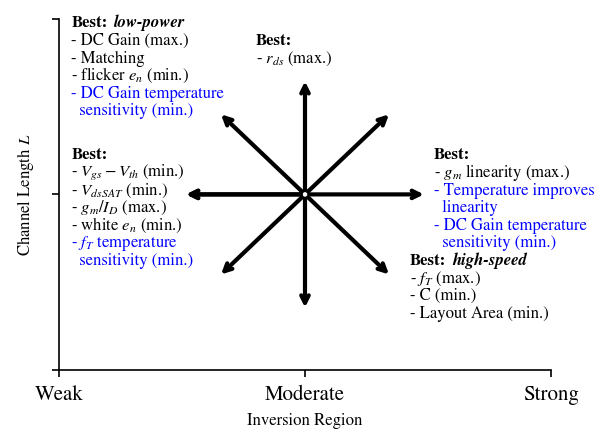
\includegraphics[width=0.8\textwidth]{tradeoffs}
	%% Creator: Matplotlib, PGF backend
%%
%% To include the figure in your LaTeX document, write
%%   \input{<filename>.pgf}
%%
%% Make sure the required packages are loaded in your preamble
%%   \usepackage{pgf}
%%
%% Figures using additional raster images can only be included by \input if
%% they are in the same directory as the main LaTeX file. For loading figures
%% from other directories you can use the `import` package
%%   \usepackage{import}
%% and then include the figures with
%%   \import{<path to file>}{<filename>.pgf}
%%
%% Matplotlib used the following preamble
%%   \usepackage{gensymb}
%%   \usepackage[utf8x]{inputenc}
%%   \usepackage[T1]{fontenc}
%%
\begingroup%
\makeatletter%
\begin{pgfpicture}%
\pgfpathrectangle{\pgfpointorigin}{\pgfqpoint{5.930000in}{3.930000in}}%
\pgfusepath{use as bounding box, clip}%
\begin{pgfscope}%
\pgfsetbuttcap%
\pgfsetmiterjoin%
\definecolor{currentfill}{rgb}{1.000000,1.000000,1.000000}%
\pgfsetfillcolor{currentfill}%
\pgfsetlinewidth{0.000000pt}%
\definecolor{currentstroke}{rgb}{1.000000,1.000000,1.000000}%
\pgfsetstrokecolor{currentstroke}%
\pgfsetdash{}{0pt}%
\pgfpathmoveto{\pgfqpoint{0.000000in}{0.000000in}}%
\pgfpathlineto{\pgfqpoint{5.930000in}{0.000000in}}%
\pgfpathlineto{\pgfqpoint{5.930000in}{3.930000in}}%
\pgfpathlineto{\pgfqpoint{0.000000in}{3.930000in}}%
\pgfpathclose%
\pgfusepath{fill}%
\end{pgfscope}%
\begin{pgfscope}%
\pgfsetbuttcap%
\pgfsetmiterjoin%
\definecolor{currentfill}{rgb}{1.000000,1.000000,1.000000}%
\pgfsetfillcolor{currentfill}%
\pgfsetlinewidth{0.000000pt}%
\definecolor{currentstroke}{rgb}{0.000000,0.000000,0.000000}%
\pgfsetstrokecolor{currentstroke}%
\pgfsetstrokeopacity{0.000000}%
\pgfsetdash{}{0pt}%
\pgfpathmoveto{\pgfqpoint{0.363168in}{0.485823in}}%
\pgfpathlineto{\pgfqpoint{5.629239in}{0.485823in}}%
\pgfpathlineto{\pgfqpoint{5.629239in}{3.806667in}}%
\pgfpathlineto{\pgfqpoint{0.363168in}{3.806667in}}%
\pgfpathclose%
\pgfusepath{fill}%
\end{pgfscope}%
\begin{pgfscope}%
\pgfsetbuttcap%
\pgfsetroundjoin%
\definecolor{currentfill}{rgb}{0.000000,0.000000,0.000000}%
\pgfsetfillcolor{currentfill}%
\pgfsetlinewidth{0.803000pt}%
\definecolor{currentstroke}{rgb}{0.000000,0.000000,0.000000}%
\pgfsetstrokecolor{currentstroke}%
\pgfsetdash{}{0pt}%
\pgfsys@defobject{currentmarker}{\pgfqpoint{0.000000in}{-0.048611in}}{\pgfqpoint{0.000000in}{0.000000in}}{%
\pgfpathmoveto{\pgfqpoint{0.000000in}{0.000000in}}%
\pgfpathlineto{\pgfqpoint{0.000000in}{-0.048611in}}%
\pgfusepath{stroke,fill}%
}%
\begin{pgfscope}%
\pgfsys@transformshift{0.363168in}{0.485823in}%
\pgfsys@useobject{currentmarker}{}%
\end{pgfscope}%
\end{pgfscope}%
\begin{pgfscope}%
\pgftext[x=0.363168in,y=0.388600in,,top]{\fontsize{10.000000}{12.000000}\selectfont Weak}%
\end{pgfscope}%
\begin{pgfscope}%
\pgfsetbuttcap%
\pgfsetroundjoin%
\definecolor{currentfill}{rgb}{0.000000,0.000000,0.000000}%
\pgfsetfillcolor{currentfill}%
\pgfsetlinewidth{0.803000pt}%
\definecolor{currentstroke}{rgb}{0.000000,0.000000,0.000000}%
\pgfsetstrokecolor{currentstroke}%
\pgfsetdash{}{0pt}%
\pgfsys@defobject{currentmarker}{\pgfqpoint{0.000000in}{-0.048611in}}{\pgfqpoint{0.000000in}{0.000000in}}{%
\pgfpathmoveto{\pgfqpoint{0.000000in}{0.000000in}}%
\pgfpathlineto{\pgfqpoint{0.000000in}{-0.048611in}}%
\pgfusepath{stroke,fill}%
}%
\begin{pgfscope}%
\pgfsys@transformshift{2.996203in}{0.485823in}%
\pgfsys@useobject{currentmarker}{}%
\end{pgfscope}%
\end{pgfscope}%
\begin{pgfscope}%
\pgftext[x=2.996203in,y=0.388600in,,top]{\fontsize{10.000000}{12.000000}\selectfont Moderate}%
\end{pgfscope}%
\begin{pgfscope}%
\pgfsetbuttcap%
\pgfsetroundjoin%
\definecolor{currentfill}{rgb}{0.000000,0.000000,0.000000}%
\pgfsetfillcolor{currentfill}%
\pgfsetlinewidth{0.803000pt}%
\definecolor{currentstroke}{rgb}{0.000000,0.000000,0.000000}%
\pgfsetstrokecolor{currentstroke}%
\pgfsetdash{}{0pt}%
\pgfsys@defobject{currentmarker}{\pgfqpoint{0.000000in}{-0.048611in}}{\pgfqpoint{0.000000in}{0.000000in}}{%
\pgfpathmoveto{\pgfqpoint{0.000000in}{0.000000in}}%
\pgfpathlineto{\pgfqpoint{0.000000in}{-0.048611in}}%
\pgfusepath{stroke,fill}%
}%
\begin{pgfscope}%
\pgfsys@transformshift{5.629239in}{0.485823in}%
\pgfsys@useobject{currentmarker}{}%
\end{pgfscope}%
\end{pgfscope}%
\begin{pgfscope}%
\pgftext[x=5.629239in,y=0.388600in,,top]{\fontsize{10.000000}{12.000000}\selectfont Strong}%
\end{pgfscope}%
\begin{pgfscope}%
\pgftext[x=2.996203in,y=0.210390in,,top]{\fontsize{9.000000}{10.800000}\selectfont Inversion Region}%
\end{pgfscope}%
\begin{pgfscope}%
\pgfsetbuttcap%
\pgfsetroundjoin%
\definecolor{currentfill}{rgb}{0.000000,0.000000,0.000000}%
\pgfsetfillcolor{currentfill}%
\pgfsetlinewidth{0.803000pt}%
\definecolor{currentstroke}{rgb}{0.000000,0.000000,0.000000}%
\pgfsetstrokecolor{currentstroke}%
\pgfsetdash{}{0pt}%
\pgfsys@defobject{currentmarker}{\pgfqpoint{-0.048611in}{0.000000in}}{\pgfqpoint{0.000000in}{0.000000in}}{%
\pgfpathmoveto{\pgfqpoint{0.000000in}{0.000000in}}%
\pgfpathlineto{\pgfqpoint{-0.048611in}{0.000000in}}%
\pgfusepath{stroke,fill}%
}%
\begin{pgfscope}%
\pgfsys@transformshift{0.363168in}{0.485823in}%
\pgfsys@useobject{currentmarker}{}%
\end{pgfscope}%
\end{pgfscope}%
\begin{pgfscope}%
\pgfsetbuttcap%
\pgfsetroundjoin%
\definecolor{currentfill}{rgb}{0.000000,0.000000,0.000000}%
\pgfsetfillcolor{currentfill}%
\pgfsetlinewidth{0.803000pt}%
\definecolor{currentstroke}{rgb}{0.000000,0.000000,0.000000}%
\pgfsetstrokecolor{currentstroke}%
\pgfsetdash{}{0pt}%
\pgfsys@defobject{currentmarker}{\pgfqpoint{-0.048611in}{0.000000in}}{\pgfqpoint{0.000000in}{0.000000in}}{%
\pgfpathmoveto{\pgfqpoint{0.000000in}{0.000000in}}%
\pgfpathlineto{\pgfqpoint{-0.048611in}{0.000000in}}%
\pgfusepath{stroke,fill}%
}%
\begin{pgfscope}%
\pgfsys@transformshift{0.363168in}{2.146245in}%
\pgfsys@useobject{currentmarker}{}%
\end{pgfscope}%
\end{pgfscope}%
\begin{pgfscope}%
\pgfsetbuttcap%
\pgfsetroundjoin%
\definecolor{currentfill}{rgb}{0.000000,0.000000,0.000000}%
\pgfsetfillcolor{currentfill}%
\pgfsetlinewidth{0.803000pt}%
\definecolor{currentstroke}{rgb}{0.000000,0.000000,0.000000}%
\pgfsetstrokecolor{currentstroke}%
\pgfsetdash{}{0pt}%
\pgfsys@defobject{currentmarker}{\pgfqpoint{-0.048611in}{0.000000in}}{\pgfqpoint{0.000000in}{0.000000in}}{%
\pgfpathmoveto{\pgfqpoint{0.000000in}{0.000000in}}%
\pgfpathlineto{\pgfqpoint{-0.048611in}{0.000000in}}%
\pgfusepath{stroke,fill}%
}%
\begin{pgfscope}%
\pgfsys@transformshift{0.363168in}{3.806667in}%
\pgfsys@useobject{currentmarker}{}%
\end{pgfscope}%
\end{pgfscope}%
\begin{pgfscope}%
\pgftext[x=0.210390in,y=2.146245in,,bottom,rotate=90.000000]{\fontsize{9.000000}{10.800000}\selectfont Channel Length \(\displaystyle L\)}%
\end{pgfscope}%
\begin{pgfscope}%
\pgfsetrectcap%
\pgfsetmiterjoin%
\pgfsetlinewidth{0.803000pt}%
\definecolor{currentstroke}{rgb}{0.000000,0.000000,0.000000}%
\pgfsetstrokecolor{currentstroke}%
\pgfsetdash{}{0pt}%
\pgfpathmoveto{\pgfqpoint{0.363168in}{0.485823in}}%
\pgfpathlineto{\pgfqpoint{0.363168in}{3.806667in}}%
\pgfusepath{stroke}%
\end{pgfscope}%
\begin{pgfscope}%
\pgfsetrectcap%
\pgfsetmiterjoin%
\pgfsetlinewidth{0.803000pt}%
\definecolor{currentstroke}{rgb}{0.000000,0.000000,0.000000}%
\pgfsetstrokecolor{currentstroke}%
\pgfsetdash{}{0pt}%
\pgfpathmoveto{\pgfqpoint{0.363168in}{0.485823in}}%
\pgfpathlineto{\pgfqpoint{5.629239in}{0.485823in}}%
\pgfusepath{stroke}%
\end{pgfscope}%
\begin{pgfscope}%
\pgfsetroundcap%
\pgfsetroundjoin%
\pgfsetlinewidth{2.007500pt}%
\definecolor{currentstroke}{rgb}{0.000000,0.000000,0.000000}%
\pgfsetstrokecolor{currentstroke}%
\pgfsetdash{}{0pt}%
\pgfpathmoveto{\pgfqpoint{4.253882in}{2.146245in}}%
\pgfpathquadraticcurveto{\pgfqpoint{3.654464in}{2.146245in}}{\pgfqpoint{3.023989in}{2.146245in}}%
\pgfusepath{stroke}%
\end{pgfscope}%
\begin{pgfscope}%
\pgfsetroundcap%
\pgfsetroundjoin%
\pgfsetlinewidth{2.007500pt}%
\definecolor{currentstroke}{rgb}{0.000000,0.000000,0.000000}%
\pgfsetstrokecolor{currentstroke}%
\pgfsetdash{}{0pt}%
\pgfpathmoveto{\pgfqpoint{4.203882in}{2.171245in}}%
\pgfpathlineto{\pgfqpoint{4.253882in}{2.146245in}}%
\pgfpathlineto{\pgfqpoint{4.203882in}{2.121245in}}%
\pgfusepath{stroke}%
\end{pgfscope}%
\begin{pgfscope}%
\pgfsetroundcap%
\pgfsetroundjoin%
\pgfsetlinewidth{2.007500pt}%
\definecolor{currentstroke}{rgb}{0.000000,0.000000,0.000000}%
\pgfsetstrokecolor{currentstroke}%
\pgfsetdash{}{0pt}%
\pgfpathmoveto{\pgfqpoint{3.882087in}{2.891109in}}%
\pgfpathquadraticcurveto{\pgfqpoint{3.461656in}{2.537604in}}{\pgfqpoint{3.017454in}{2.164112in}}%
\pgfusepath{stroke}%
\end{pgfscope}%
\begin{pgfscope}%
\pgfsetroundcap%
\pgfsetroundjoin%
\pgfsetlinewidth{2.007500pt}%
\definecolor{currentstroke}{rgb}{0.000000,0.000000,0.000000}%
\pgfsetstrokecolor{currentstroke}%
\pgfsetdash{}{0pt}%
\pgfpathmoveto{\pgfqpoint{3.827728in}{2.878066in}}%
\pgfpathlineto{\pgfqpoint{3.882087in}{2.891109in}}%
\pgfpathlineto{\pgfqpoint{3.859906in}{2.839796in}}%
\pgfusepath{stroke}%
\end{pgfscope}%
\begin{pgfscope}%
\pgfsetroundcap%
\pgfsetroundjoin%
\pgfsetlinewidth{2.007500pt}%
\definecolor{currentstroke}{rgb}{0.000000,0.000000,0.000000}%
\pgfsetstrokecolor{currentstroke}%
\pgfsetdash{}{0pt}%
\pgfpathmoveto{\pgfqpoint{2.996203in}{3.194351in}}%
\pgfpathquadraticcurveto{\pgfqpoint{2.996203in}{2.699708in}}{\pgfqpoint{2.996203in}{2.174008in}}%
\pgfusepath{stroke}%
\end{pgfscope}%
\begin{pgfscope}%
\pgfsetroundcap%
\pgfsetroundjoin%
\pgfsetlinewidth{2.007500pt}%
\definecolor{currentstroke}{rgb}{0.000000,0.000000,0.000000}%
\pgfsetstrokecolor{currentstroke}%
\pgfsetdash{}{0pt}%
\pgfpathmoveto{\pgfqpoint{2.971203in}{3.144351in}}%
\pgfpathlineto{\pgfqpoint{2.996203in}{3.194351in}}%
\pgfpathlineto{\pgfqpoint{3.021203in}{3.144351in}}%
\pgfusepath{stroke}%
\end{pgfscope}%
\begin{pgfscope}%
\pgfsetroundcap%
\pgfsetroundjoin%
\pgfsetlinewidth{2.007500pt}%
\definecolor{currentstroke}{rgb}{0.000000,0.000000,0.000000}%
\pgfsetstrokecolor{currentstroke}%
\pgfsetdash{}{0pt}%
\pgfpathmoveto{\pgfqpoint{1.738524in}{2.146245in}}%
\pgfpathquadraticcurveto{\pgfqpoint{2.337942in}{2.146245in}}{\pgfqpoint{2.968417in}{2.146245in}}%
\pgfusepath{stroke}%
\end{pgfscope}%
\begin{pgfscope}%
\pgfsetroundcap%
\pgfsetroundjoin%
\pgfsetlinewidth{2.007500pt}%
\definecolor{currentstroke}{rgb}{0.000000,0.000000,0.000000}%
\pgfsetstrokecolor{currentstroke}%
\pgfsetdash{}{0pt}%
\pgfpathmoveto{\pgfqpoint{1.788524in}{2.121245in}}%
\pgfpathlineto{\pgfqpoint{1.738524in}{2.146245in}}%
\pgfpathlineto{\pgfqpoint{1.788524in}{2.171245in}}%
\pgfusepath{stroke}%
\end{pgfscope}%
\begin{pgfscope}%
\pgfsetroundcap%
\pgfsetroundjoin%
\pgfsetlinewidth{2.007500pt}%
\definecolor{currentstroke}{rgb}{0.000000,0.000000,0.000000}%
\pgfsetstrokecolor{currentstroke}%
\pgfsetdash{}{0pt}%
\pgfpathmoveto{\pgfqpoint{2.110319in}{2.891109in}}%
\pgfpathquadraticcurveto{\pgfqpoint{2.530751in}{2.537604in}}{\pgfqpoint{2.974953in}{2.164112in}}%
\pgfusepath{stroke}%
\end{pgfscope}%
\begin{pgfscope}%
\pgfsetroundcap%
\pgfsetroundjoin%
\pgfsetlinewidth{2.007500pt}%
\definecolor{currentstroke}{rgb}{0.000000,0.000000,0.000000}%
\pgfsetstrokecolor{currentstroke}%
\pgfsetdash{}{0pt}%
\pgfpathmoveto{\pgfqpoint{2.132500in}{2.839796in}}%
\pgfpathlineto{\pgfqpoint{2.110319in}{2.891109in}}%
\pgfpathlineto{\pgfqpoint{2.164678in}{2.878066in}}%
\pgfusepath{stroke}%
\end{pgfscope}%
\begin{pgfscope}%
\pgfsetroundcap%
\pgfsetroundjoin%
\pgfsetlinewidth{2.007500pt}%
\definecolor{currentstroke}{rgb}{0.000000,0.000000,0.000000}%
\pgfsetstrokecolor{currentstroke}%
\pgfsetdash{}{0pt}%
\pgfpathmoveto{\pgfqpoint{1.738524in}{2.146245in}}%
\pgfpathquadraticcurveto{\pgfqpoint{2.337942in}{2.146245in}}{\pgfqpoint{2.968417in}{2.146245in}}%
\pgfusepath{stroke}%
\end{pgfscope}%
\begin{pgfscope}%
\pgfsetroundcap%
\pgfsetroundjoin%
\pgfsetlinewidth{2.007500pt}%
\definecolor{currentstroke}{rgb}{0.000000,0.000000,0.000000}%
\pgfsetstrokecolor{currentstroke}%
\pgfsetdash{}{0pt}%
\pgfpathmoveto{\pgfqpoint{1.788524in}{2.121245in}}%
\pgfpathlineto{\pgfqpoint{1.738524in}{2.146245in}}%
\pgfpathlineto{\pgfqpoint{1.788524in}{2.171245in}}%
\pgfusepath{stroke}%
\end{pgfscope}%
\begin{pgfscope}%
\pgfsetroundcap%
\pgfsetroundjoin%
\pgfsetlinewidth{2.007500pt}%
\definecolor{currentstroke}{rgb}{0.000000,0.000000,0.000000}%
\pgfsetstrokecolor{currentstroke}%
\pgfsetdash{}{0pt}%
\pgfpathmoveto{\pgfqpoint{2.110319in}{1.401380in}}%
\pgfpathquadraticcurveto{\pgfqpoint{2.530751in}{1.754885in}}{\pgfqpoint{2.974953in}{2.128377in}}%
\pgfusepath{stroke}%
\end{pgfscope}%
\begin{pgfscope}%
\pgfsetroundcap%
\pgfsetroundjoin%
\pgfsetlinewidth{2.007500pt}%
\definecolor{currentstroke}{rgb}{0.000000,0.000000,0.000000}%
\pgfsetstrokecolor{currentstroke}%
\pgfsetdash{}{0pt}%
\pgfpathmoveto{\pgfqpoint{2.164678in}{1.414423in}}%
\pgfpathlineto{\pgfqpoint{2.110319in}{1.401380in}}%
\pgfpathlineto{\pgfqpoint{2.132500in}{1.452693in}}%
\pgfusepath{stroke}%
\end{pgfscope}%
\begin{pgfscope}%
\pgfsetroundcap%
\pgfsetroundjoin%
\pgfsetlinewidth{2.007500pt}%
\definecolor{currentstroke}{rgb}{0.000000,0.000000,0.000000}%
\pgfsetstrokecolor{currentstroke}%
\pgfsetdash{}{0pt}%
\pgfpathmoveto{\pgfqpoint{2.996203in}{1.098138in}}%
\pgfpathquadraticcurveto{\pgfqpoint{2.996203in}{1.592782in}}{\pgfqpoint{2.996203in}{2.118482in}}%
\pgfusepath{stroke}%
\end{pgfscope}%
\begin{pgfscope}%
\pgfsetroundcap%
\pgfsetroundjoin%
\pgfsetlinewidth{2.007500pt}%
\definecolor{currentstroke}{rgb}{0.000000,0.000000,0.000000}%
\pgfsetstrokecolor{currentstroke}%
\pgfsetdash{}{0pt}%
\pgfpathmoveto{\pgfqpoint{3.021203in}{1.148138in}}%
\pgfpathlineto{\pgfqpoint{2.996203in}{1.098138in}}%
\pgfpathlineto{\pgfqpoint{2.971203in}{1.148138in}}%
\pgfusepath{stroke}%
\end{pgfscope}%
\begin{pgfscope}%
\pgfsetroundcap%
\pgfsetroundjoin%
\pgfsetlinewidth{2.007500pt}%
\definecolor{currentstroke}{rgb}{0.000000,0.000000,0.000000}%
\pgfsetstrokecolor{currentstroke}%
\pgfsetdash{}{0pt}%
\pgfpathmoveto{\pgfqpoint{3.882087in}{1.401380in}}%
\pgfpathquadraticcurveto{\pgfqpoint{3.461656in}{1.754885in}}{\pgfqpoint{3.017454in}{2.128377in}}%
\pgfusepath{stroke}%
\end{pgfscope}%
\begin{pgfscope}%
\pgfsetroundcap%
\pgfsetroundjoin%
\pgfsetlinewidth{2.007500pt}%
\definecolor{currentstroke}{rgb}{0.000000,0.000000,0.000000}%
\pgfsetstrokecolor{currentstroke}%
\pgfsetdash{}{0pt}%
\pgfpathmoveto{\pgfqpoint{3.859906in}{1.452693in}}%
\pgfpathlineto{\pgfqpoint{3.882087in}{1.401380in}}%
\pgfpathlineto{\pgfqpoint{3.827728in}{1.414423in}}%
\pgfusepath{stroke}%
\end{pgfscope}%
\begin{pgfscope}%
\pgftext[x=0.494819in,y=2.478329in,left,base]{\fontsize{9.000000}{10.800000}\bfseries\selectfont Best:}%
\end{pgfscope}%
\begin{pgfscope}%
\pgftext[x=0.494819in,y=2.312287in,left,base]{\fontsize{9.000000}{10.800000}\selectfont - \(\displaystyle V_{gs}-V_{th}\) (min.)}%
\end{pgfscope}%
\begin{pgfscope}%
\pgftext[x=0.494819in,y=2.146245in,left,base]{\fontsize{9.000000}{10.800000}\selectfont - \(\displaystyle V_{dsSAT}\) (min.)}%
\end{pgfscope}%
\begin{pgfscope}%
\pgftext[x=0.494819in,y=1.980202in,left,base]{\fontsize{9.000000}{10.800000}\selectfont - \(\displaystyle g_m/I_D\) (max.)}%
\end{pgfscope}%
\begin{pgfscope}%
\pgftext[x=0.494819in,y=1.814160in,left,base]{\fontsize{9.000000}{10.800000}\selectfont - white \(\displaystyle e_n\) (min.)}%
\end{pgfscope}%
\begin{pgfscope}%
\definecolor{textcolor}{rgb}{0.000000,0.000000,1.000000}%
\pgfsetstrokecolor{textcolor}%
\pgfsetfillcolor{textcolor}%
\pgftext[x=0.494819in,y=1.648118in,left,base]{\color{textcolor}\fontsize{9.000000}{10.800000}\selectfont - \(\displaystyle f_T\) temperature}%
\end{pgfscope}%
\begin{pgfscope}%
\definecolor{textcolor}{rgb}{0.000000,0.000000,1.000000}%
\pgfsetstrokecolor{textcolor}%
\pgfsetfillcolor{textcolor}%
\pgftext[x=0.494819in,y=1.482076in,left,base]{\color{textcolor}\fontsize{9.000000}{10.800000}\selectfont   sensitivity (min.)}%
\end{pgfscope}%
\begin{pgfscope}%
\pgftext[x=0.494819in,y=3.723646in,left,base]{\fontsize{9.000000}{10.800000}\bfseries\selectfont Best:}%
\end{pgfscope}%
\begin{pgfscope}%
\pgftext[x=0.955601in,y=3.723646in,left,base]{\fontsize{9.000000}{10.800000}\itshape\bfseries\selectfont low-power}%
\end{pgfscope}%
\begin{pgfscope}%
\pgftext[x=0.494819in,y=3.557603in,left,base]{\fontsize{9.000000}{10.800000}\selectfont - DC Gain (max.)}%
\end{pgfscope}%
\begin{pgfscope}%
\pgftext[x=0.494819in,y=3.391561in,left,base]{\fontsize{9.000000}{10.800000}\selectfont - Matching}%
\end{pgfscope}%
\begin{pgfscope}%
\pgftext[x=0.494819in,y=3.225519in,left,base]{\fontsize{9.000000}{10.800000}\selectfont - flicker \(\displaystyle e_n\) (min.)}%
\end{pgfscope}%
\begin{pgfscope}%
\definecolor{textcolor}{rgb}{0.000000,0.000000,1.000000}%
\pgfsetstrokecolor{textcolor}%
\pgfsetfillcolor{textcolor}%
\pgftext[x=0.494819in,y=3.059477in,left,base]{\color{textcolor}\fontsize{9.000000}{10.800000}\selectfont - DC Gain temperature}%
\end{pgfscope}%
\begin{pgfscope}%
\definecolor{textcolor}{rgb}{0.000000,0.000000,1.000000}%
\pgfsetstrokecolor{textcolor}%
\pgfsetfillcolor{textcolor}%
\pgftext[x=0.494819in,y=2.893435in,left,base]{\color{textcolor}\fontsize{9.000000}{10.800000}\selectfont   sensitivity (min.)}%
\end{pgfscope}%
\begin{pgfscope}%
\pgftext[x=2.469596in,y=3.557603in,left,base]{\fontsize{9.000000}{10.800000}\bfseries\selectfont Best:}%
\end{pgfscope}%
\begin{pgfscope}%
\pgftext[x=2.469596in,y=3.391561in,left,base]{\fontsize{9.000000}{10.800000}\selectfont - \(\displaystyle r_{ds}\) (max.)}%
\end{pgfscope}%
\begin{pgfscope}%
\pgftext[x=4.378547in,y=2.478329in,left,base]{\fontsize{9.000000}{10.800000}\bfseries\selectfont Best:}%
\end{pgfscope}%
\begin{pgfscope}%
\pgftext[x=4.378547in,y=2.312287in,left,base]{\fontsize{9.000000}{10.800000}\selectfont - \(\displaystyle g_m\) linearity (max.)}%
\end{pgfscope}%
\begin{pgfscope}%
\definecolor{textcolor}{rgb}{0.000000,0.000000,1.000000}%
\pgfsetstrokecolor{textcolor}%
\pgfsetfillcolor{textcolor}%
\pgftext[x=4.378547in,y=2.146245in,left,base]{\color{textcolor}\fontsize{9.000000}{10.800000}\selectfont - Temperature improves}%
\end{pgfscope}%
\begin{pgfscope}%
\definecolor{textcolor}{rgb}{0.000000,0.000000,1.000000}%
\pgfsetstrokecolor{textcolor}%
\pgfsetfillcolor{textcolor}%
\pgftext[x=4.378547in,y=1.980202in,left,base]{\color{textcolor}\fontsize{9.000000}{10.800000}\selectfont   linearity}%
\end{pgfscope}%
\begin{pgfscope}%
\definecolor{textcolor}{rgb}{0.000000,0.000000,1.000000}%
\pgfsetstrokecolor{textcolor}%
\pgfsetfillcolor{textcolor}%
\pgftext[x=4.378547in,y=1.814160in,left,base]{\color{textcolor}\fontsize{9.000000}{10.800000}\selectfont - DC Gain temperature}%
\end{pgfscope}%
\begin{pgfscope}%
\definecolor{textcolor}{rgb}{0.000000,0.000000,1.000000}%
\pgfsetstrokecolor{textcolor}%
\pgfsetfillcolor{textcolor}%
\pgftext[x=4.378547in,y=1.648118in,left,base]{\color{textcolor}\fontsize{9.000000}{10.800000}\selectfont   sensitivity (min.)}%
\end{pgfscope}%
\begin{pgfscope}%
\pgftext[x=4.115243in,y=1.482076in,left,base]{\fontsize{9.000000}{10.800000}\bfseries\selectfont Best:}%
\end{pgfscope}%
\begin{pgfscope}%
\pgftext[x=4.576025in,y=1.482076in,left,base]{\fontsize{9.000000}{10.800000}\itshape\bfseries\selectfont high-speed}%
\end{pgfscope}%
\begin{pgfscope}%
\pgftext[x=4.115243in,y=1.316034in,left,base]{\fontsize{9.000000}{10.800000}\selectfont - \(\displaystyle f_T\) (max.)}%
\end{pgfscope}%
\begin{pgfscope}%
\pgftext[x=4.115243in,y=1.149991in,left,base]{\fontsize{9.000000}{10.800000}\selectfont - C (min.)}%
\end{pgfscope}%
\begin{pgfscope}%
\pgftext[x=4.115243in,y=0.983949in,left,base]{\fontsize{9.000000}{10.800000}\selectfont - Layout Area (min.)}%
\end{pgfscope}%
\end{pgfpicture}%
\makeatother%
\endgroup%

	\caption{Trade-offs in circuit performance as a function of the channel length L and the Inversion level}
	\label{fig:tradeoffs}
\end{figure}

The design of high-resolution and high-speed OTA is the bottleneck of high-performance ADCs: the accuracy of switched capacitor circuits depending on them. Based on this analysis, the temperature affects the speeds of transistors, and it cannot be prevented. While the gain could be stable over temperature, this can only be ensured for transistors in weak inversion. In this mode, then a single transistor of the technology cannot exceed 200 MHz.
Therefore, the biasing circuitry would be in weak-moderate inversion region with large-L. And high-speed differential pairs should be in moderate-strong inversion region with small-L.

\clearpage
\section{High Temperature ADCs}     % section 2.6
\label{sec:high-temp-adc}
Until now, only standard topologies and recent progress among them have been reported. High-speed and medium to high-resolution converters are an extended topic. With the temperature constraints previously explained, this topic is fairly reduced since only a few papers address this challenge. This subsection discusses work published to cope with the high temperature in ADCs.

From a high-level point of view, solutions with fewer sensitive components over a wide temperature range are preferred. As the temperature deeply impacts the analog electronics more than a synchronous digital, SAR without amplifier or \(\Delta\Sigma \) ADCs are less demanding on analog accuracy. Thus, they are popular architectures among many for harsh environment applications.

\subsection{SAR}
Even though SAR have a limited number of active components, the resolution of SAR exhibits a limiting factor temperature dependent. Indeed, the temperature increase raises the leakage current exponentially which also discharge capacitors faster. For a DAC based on poly-resistors having the lowest thermal variations, the leakage currents alter the voltage across them. Over a wide temperature range, SAR ADCs are only used as a small sub-ADC or as a low-resolution ADC\@. % while in commercial range http://cds.linear.com/docs/en/datasheet/250032fb.pdf up to 32-bits

In the work of Rahman~\textit{et al.}~\cite{Rahman2017}, the ADC consists in an 8-bits R-2R poly-resistor DAC driven by a binary search algorithm logic from 25\(\degree \)C to 300\(\degree \)C. Poly-resistors have been chosen for their lowest temperature coefficient in the technology while the comparator and the logic are implemented in SiC FET transistors. The large-bandgap of SiC reduces the leakage currents. Despite this, the resolution is limited to 8-bits which reveal how important is the leakage currents. Experimental results highlight the fact that ADCs have a better linearity at high temperatures when the dominant factor is switches non-linearity.

Recently, an overview of an analysis of latched-comparators performance, considering process variability and temperature variation from -40\(\degree \)C to 175\(\degree \)C was presented. Fonseca ~\textit{et al.}~\cite{Fonseca2018} have extended such analysis to the metastability and performance metrics variation of SAR ADCs. Besides the known advantages of the Double-Tail comparator, Fonseca's work has demonstrated that such a comparator has a serious drawback under harsh environments. Finally, post-layout results have been presented. Once the SAR ADC is calibrated and operated at a frequency of around 100 MHz, the ADC performance can be maintained in a wide temperature range. Both SA-SAR and DT-SAR ADC achieve an ENOB of 9.8 bits, which is reduced to 9.6 bits in high-temperature operation.

\subsection{$\Delta\Sigma$}
\(\Delta\Sigma \) modulator is known to be resilient to analog circuit impairment by transferring the complexity to the digital domain. Nevertheless, the leakage current turns out to be the main contributor to a significant voltage drop in the switched capacitor circuit. Due to this reason, a fully differential ADC lower the impact on the accuracy due to the leakage difference between the positive and negative branch~\cite{Davis2003}. For low-OSR modulator, experiments have demonstrated that single-stage modulator is more resistant to high-temperature than MASH cascaded one. The latter underwent severe drift of the amplifier output common-mode voltage up to 255\(\degree \)C degrading overall performance of MASH solutions. The $\Delta\Sigma$ modulation reaches a high resolution for a large temperature range. Such results were demonstrated either in a bulk technology~\cite{Davis2003} or in an SOI technology~\cite{Ericson2004}.

\subsection{Pipelined}
Keeping aside these architectures, a pipelined based on Flip-Around MDAC has been proved to work under the stringent temperature range from -180\(\degree \)C to 120\(\degree \)C in a bulk technology~\cite{Yao2010}. At negative temperatures, the amplifier is prone to a transconductance reduction and a reduced gain owed to the threshold voltage increased. Large W/L transistors reduce the threshold shift while they improve the matching property. As expected, the pipelined architecture with a 5 MHz sampling frequency in~\cite{Yao2010} is faster in comparison to $\Delta\Sigma$ ADCs for a resolution of 12-bits.

\subsection{Mixed Architecture}
In the implementation of a CMOS temperature sensor in the -40\(\degree \)C to 125\(\degree \)C range, Souri~\textit{et al.} present a second-order Zoom-ADC~\cite{Souri2014}. A capacitive SAR ADC performs a coarse conversion to determine a rough estimate followed by a fine conversion by a second order Incremental-\(\Delta\Sigma \) converter. The SAR first proposal allows one to remove the sample and hold introducing large error as the temperature increase. Using well-known robust sub-ADCs, only single temperature point calibration effectively trims inaccuracy over the wide temperature range. This ADC achieves a resolution of 16-bits, and a power consumption drastically low of 8.6 $\mu$W.

The table~\ref{table:algo_comparison_table} compares performance of converters in prior art.
\begin{table}[htp]
	\caption{High-Temperature ADC in the literature}
	\centering
	\label{table:high_temp_comparison_table}
	\begin{tabular}{L{3.5\charwidth} R{7.5\charwidth} R{4\charwidth} R{9.5\charwidth} R{5\charwidth} R{11.5\charwidth} R{6\charwidth} R{8\charwidth} C{4\charwidth}}
		\toprule
		Ref. & Archi. & \multicolumn{2}{c}{Technology [nm]}  & \(F_{snyq} \) [kHz] & Temperature Range & Supply [V] & Power [mW] & Res. [bits] \\
		\midrule
		\cite{Fonseca2018}  & SAR                  & 180  &SOI CMOS   & 5000 & -40\(\degree \)C--175\(\degree \)C &  1.8 &  0.35& 9.8 \\
		\cite{Rahman2017}  & SAR                   & 1200 & SiC       &   64 & 25\(\degree \)C--300\(\degree \)C   &  5   &   1.4 &  8 \\
		\cite{Davis2003}   & \(\Delta\Sigma \)     & 1500 & Bulk CMOS &    1 & 25\(\degree \)C--225\(\degree \)C   &  5   &    NA & 14 \\
		\cite{Ericson2004} & \(\Delta\Sigma \)     &  500 & SOI CMOS  &    2 & 25\(\degree \)C--225\(\degree \)C   &  3.3 &    NA & 16 \\
		\cite{Yao2010}     & pipe.                 &  500 & Bulk CMOS & 5000 & -180\(\degree \)C--120\(\degree \)C &  3.3 &  30.4 & 12 \\
		\cite{Souri2014}   & SAR+\(\Delta\Sigma \) &  160 & Bulk CMOS &   NA & -55\(\degree \)C--125\(\degree \)C  &  1.8 &  8.6$\times10^{-3}$ & 16 \\
		\bottomrule
	\end{tabular}
\end{table}

Despite the heavy work on the temperature to enhance ADCs, the following references achieve valuable results at high temperature but disregard what happen at negative temperature~\cite{Rahman2017,Davis2003,Ericson2004}. It is worth to point out that high-resolution converter is based on \(\Delta\Sigma \) modulation such as in the work of~\cite{Souri2014,Davis2003,Ericson2004}. The ADC performance reliability can be maintained in a wide temperature range according to \cite{Fonseca2018}. Finally, the closest ADC from our expectation is a hybrid architecture presented in~\cite{Souri2014}. Nevertheless, the latter operates for a reduced temperature range which does not exceed 125\(\degree \)C. A new solution shall be considered.
% Challenges in conventional ADC
%%!TEX root = ../thesis.tex
% chktex-file 1
% chktex-file 24
%*******************************************************************************
%****************************** Second Chapter *********************************
%*******************************************************************************

\chapter{Analogue Insight for High-Temperature ICs}
\label{sec:temperature-analogue}
% **************************** Define Graphics Path **************************
\ifpdf
    \graphicspath{{Chapter2/Figs/Raster/}{Chapter2/Figs/PDF/}{Chapter2/Figs/}}
\else
    \graphicspath{{Chapter2/Figs/Vector/}{Chapter2/Figs/}}
\fi

There are many industries such as the automotive that requires sensors and other mixed signal electronics capable of operating within an extreme temperature range from -40 \(\degree \)C to 175 \(\degree \)C. At high temperatures, transistors suffer from several defects that degrade their performance and the system performance.

Over such a large temperature range, phenomena due to temperature should be considered early in the design and in the research. The background presented within this section discusses the impact of the temperature at the device and circuit level. Moreover the material dependences, as well as transistors variation with respect to the temperature, are illustrated with the CMOS XT018 technology results. % this last point should be discussed with JVE and PLA to respect technical disclosure.
\nomenclature[z]{CMOS}{Complementary Metal-Oxide-Semiconductor}

\section{Thermal Dependence of Semiconductor}
\subsection{Energy Band Gap}        % section 2.1
In solid-state physics, the energy band gap is the energy required to supercharge an electron from the valence band to the conduction band. Any extra energy, wherever does it come from, will change the thermodynamic equilibrium of the solid. As a consequence, electrons' state repartition in the valence and conduction band vary with the temperature according to the Fermi-Dirac distribution. In turn, tightly linked to this distribution, the band gap energy changes with respect to the temperature.

Even if, the fitting equations of low-temperature data have been greatly discussed~\cite{Varshni1967,Allen1976,Manoogian1979,Donnell1991}, the trends of the bandgap energy required over temperature is modelled easily by the Varshni equation~(\ref{eqn:Varshni}) in~\cite{Varshni1967}
\begin{equation}
\label{eqn:Varshni}
E_g(T) = E_g(T_0) - \alpha \frac{T^2}{T+\beta}
\end{equation}
\(E_g(T_0) \) represents the band gap energy required at the temperature of reference \(T_0 \), while \(\alpha \) and \(\beta \) are fitting constants. For the Silicon, with \(T_0 = \)300 K, \(\alpha \) and \(\beta \) are respectively 0.473 meV/K and 636K. \(E_g(T_0) \) is given to be 1.166 eV. The change over the temperature range of interest is given by the \figurename~\ref{fig:bandgap} where the derivative with respect to the temperature is about 400 ppm/K.
\nomenclature[A-Eg]{$E_g$}{Bandgap Energy}
\nomenclature[A-K]{$K$}{degree Kelvin}

\begin{figure}[!ht]
    \centering
    %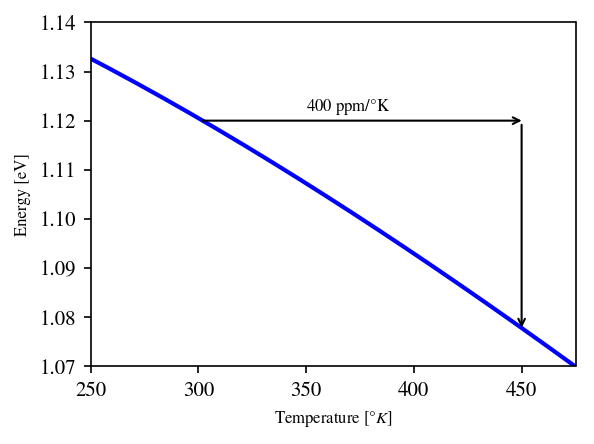
\includegraphics[width=0.6\textwidth]{bandgap}
    %% Creator: Matplotlib, PGF backend
%%
%% To include the figure in your LaTeX document, write
%%   \input{<filename>.pgf}
%%
%% Make sure the required packages are loaded in your preamble
%%   \usepackage{pgf}
%%
%% Figures using additional raster images can only be included by \input if
%% they are in the same directory as the main LaTeX file. For loading figures
%% from other directories you can use the `import` package
%%   \usepackage{import}
%% and then include the figures with
%%   \import{<path to file>}{<filename>.pgf}
%%
%% Matplotlib used the following preamble
%%   \usepackage{gensymb}
%%   \usepackage[utf8x]{inputenc}
%%   \usepackage[T1]{fontenc}
%%
\begingroup%
\makeatletter%
\begin{pgfpicture}%
\pgfpathrectangle{\pgfpointorigin}{\pgfqpoint{3.930000in}{2.930000in}}%
\pgfusepath{use as bounding box, clip}%
\begin{pgfscope}%
\pgfsetbuttcap%
\pgfsetmiterjoin%
\definecolor{currentfill}{rgb}{1.000000,1.000000,1.000000}%
\pgfsetfillcolor{currentfill}%
\pgfsetlinewidth{0.000000pt}%
\definecolor{currentstroke}{rgb}{1.000000,1.000000,1.000000}%
\pgfsetstrokecolor{currentstroke}%
\pgfsetdash{}{0pt}%
\pgfpathmoveto{\pgfqpoint{0.000000in}{0.000000in}}%
\pgfpathlineto{\pgfqpoint{3.930000in}{0.000000in}}%
\pgfpathlineto{\pgfqpoint{3.930000in}{2.930000in}}%
\pgfpathlineto{\pgfqpoint{0.000000in}{2.930000in}}%
\pgfpathclose%
\pgfusepath{fill}%
\end{pgfscope}%
\begin{pgfscope}%
\pgfsetbuttcap%
\pgfsetmiterjoin%
\definecolor{currentfill}{rgb}{1.000000,1.000000,1.000000}%
\pgfsetfillcolor{currentfill}%
\pgfsetlinewidth{0.000000pt}%
\definecolor{currentstroke}{rgb}{0.000000,0.000000,0.000000}%
\pgfsetstrokecolor{currentstroke}%
\pgfsetstrokeopacity{0.000000}%
\pgfsetdash{}{0pt}%
\pgfpathmoveto{\pgfqpoint{0.624662in}{0.506458in}}%
\pgfpathlineto{\pgfqpoint{3.806667in}{0.506458in}}%
\pgfpathlineto{\pgfqpoint{3.806667in}{2.782172in}}%
\pgfpathlineto{\pgfqpoint{0.624662in}{2.782172in}}%
\pgfpathclose%
\pgfusepath{fill}%
\end{pgfscope}%
\begin{pgfscope}%
\pgfsetbuttcap%
\pgfsetroundjoin%
\definecolor{currentfill}{rgb}{0.000000,0.000000,0.000000}%
\pgfsetfillcolor{currentfill}%
\pgfsetlinewidth{0.803000pt}%
\definecolor{currentstroke}{rgb}{0.000000,0.000000,0.000000}%
\pgfsetstrokecolor{currentstroke}%
\pgfsetdash{}{0pt}%
\pgfsys@defobject{currentmarker}{\pgfqpoint{0.000000in}{-0.048611in}}{\pgfqpoint{0.000000in}{0.000000in}}{%
\pgfpathmoveto{\pgfqpoint{0.000000in}{0.000000in}}%
\pgfpathlineto{\pgfqpoint{0.000000in}{-0.048611in}}%
\pgfusepath{stroke,fill}%
}%
\begin{pgfscope}%
\pgfsys@transformshift{0.624662in}{0.506458in}%
\pgfsys@useobject{currentmarker}{}%
\end{pgfscope}%
\end{pgfscope}%
\begin{pgfscope}%
\pgftext[x=0.624662in,y=0.409236in,,top]{\fontsize{12.000000}{14.000000}\selectfont \(\displaystyle 250\)}%
\end{pgfscope}%
\begin{pgfscope}%
\pgfsetbuttcap%
\pgfsetroundjoin%
\definecolor{currentfill}{rgb}{0.000000,0.000000,0.000000}%
\pgfsetfillcolor{currentfill}%
\pgfsetlinewidth{0.803000pt}%
\definecolor{currentstroke}{rgb}{0.000000,0.000000,0.000000}%
\pgfsetstrokecolor{currentstroke}%
\pgfsetdash{}{0pt}%
\pgfsys@defobject{currentmarker}{\pgfqpoint{0.000000in}{-0.048611in}}{\pgfqpoint{0.000000in}{0.000000in}}{%
\pgfpathmoveto{\pgfqpoint{0.000000in}{0.000000in}}%
\pgfpathlineto{\pgfqpoint{0.000000in}{-0.048611in}}%
\pgfusepath{stroke,fill}%
}%
\begin{pgfscope}%
\pgfsys@transformshift{1.331774in}{0.506458in}%
\pgfsys@useobject{currentmarker}{}%
\end{pgfscope}%
\end{pgfscope}%
\begin{pgfscope}%
\pgftext[x=1.331774in,y=0.409236in,,top]{\fontsize{12.000000}{14.000000}\selectfont \(\displaystyle 300\)}%
\end{pgfscope}%
\begin{pgfscope}%
\pgfsetbuttcap%
\pgfsetroundjoin%
\definecolor{currentfill}{rgb}{0.000000,0.000000,0.000000}%
\pgfsetfillcolor{currentfill}%
\pgfsetlinewidth{0.803000pt}%
\definecolor{currentstroke}{rgb}{0.000000,0.000000,0.000000}%
\pgfsetstrokecolor{currentstroke}%
\pgfsetdash{}{0pt}%
\pgfsys@defobject{currentmarker}{\pgfqpoint{0.000000in}{-0.048611in}}{\pgfqpoint{0.000000in}{0.000000in}}{%
\pgfpathmoveto{\pgfqpoint{0.000000in}{0.000000in}}%
\pgfpathlineto{\pgfqpoint{0.000000in}{-0.048611in}}%
\pgfusepath{stroke,fill}%
}%
\begin{pgfscope}%
\pgfsys@transformshift{2.038886in}{0.506458in}%
\pgfsys@useobject{currentmarker}{}%
\end{pgfscope}%
\end{pgfscope}%
\begin{pgfscope}%
\pgftext[x=2.038886in,y=0.409236in,,top]{\fontsize{12.000000}{14.000000}\selectfont \(\displaystyle 350\)}%
\end{pgfscope}%
\begin{pgfscope}%
\pgfsetbuttcap%
\pgfsetroundjoin%
\definecolor{currentfill}{rgb}{0.000000,0.000000,0.000000}%
\pgfsetfillcolor{currentfill}%
\pgfsetlinewidth{0.803000pt}%
\definecolor{currentstroke}{rgb}{0.000000,0.000000,0.000000}%
\pgfsetstrokecolor{currentstroke}%
\pgfsetdash{}{0pt}%
\pgfsys@defobject{currentmarker}{\pgfqpoint{0.000000in}{-0.048611in}}{\pgfqpoint{0.000000in}{0.000000in}}{%
\pgfpathmoveto{\pgfqpoint{0.000000in}{0.000000in}}%
\pgfpathlineto{\pgfqpoint{0.000000in}{-0.048611in}}%
\pgfusepath{stroke,fill}%
}%
\begin{pgfscope}%
\pgfsys@transformshift{2.745998in}{0.506458in}%
\pgfsys@useobject{currentmarker}{}%
\end{pgfscope}%
\end{pgfscope}%
\begin{pgfscope}%
\pgftext[x=2.745998in,y=0.409236in,,top]{\fontsize{12.000000}{14.000000}\selectfont \(\displaystyle 400\)}%
\end{pgfscope}%
\begin{pgfscope}%
\pgfsetbuttcap%
\pgfsetroundjoin%
\definecolor{currentfill}{rgb}{0.000000,0.000000,0.000000}%
\pgfsetfillcolor{currentfill}%
\pgfsetlinewidth{0.803000pt}%
\definecolor{currentstroke}{rgb}{0.000000,0.000000,0.000000}%
\pgfsetstrokecolor{currentstroke}%
\pgfsetdash{}{0pt}%
\pgfsys@defobject{currentmarker}{\pgfqpoint{0.000000in}{-0.048611in}}{\pgfqpoint{0.000000in}{0.000000in}}{%
\pgfpathmoveto{\pgfqpoint{0.000000in}{0.000000in}}%
\pgfpathlineto{\pgfqpoint{0.000000in}{-0.048611in}}%
\pgfusepath{stroke,fill}%
}%
\begin{pgfscope}%
\pgfsys@transformshift{3.453111in}{0.506458in}%
\pgfsys@useobject{currentmarker}{}%
\end{pgfscope}%
\end{pgfscope}%
\begin{pgfscope}%
\pgftext[x=3.453111in,y=0.409236in,,top]{\fontsize{12.000000}{14.000000}\selectfont \(\displaystyle 450\)}%
\end{pgfscope}%
\begin{pgfscope}%
\pgftext[x=2.215664in,y=0.231025in,,top]{\fontsize{10.000000}{12.00000}\selectfont Temperature [K]}%
\end{pgfscope}%
\begin{pgfscope}%
\pgfsetbuttcap%
\pgfsetroundjoin%
\definecolor{currentfill}{rgb}{0.000000,0.000000,0.000000}%
\pgfsetfillcolor{currentfill}%
\pgfsetlinewidth{0.803000pt}%
\definecolor{currentstroke}{rgb}{0.000000,0.000000,0.000000}%
\pgfsetstrokecolor{currentstroke}%
\pgfsetdash{}{0pt}%
\pgfsys@defobject{currentmarker}{\pgfqpoint{-0.048611in}{0.000000in}}{\pgfqpoint{0.000000in}{0.000000in}}{%
\pgfpathmoveto{\pgfqpoint{0.000000in}{0.000000in}}%
\pgfpathlineto{\pgfqpoint{-0.048611in}{0.000000in}}%
\pgfusepath{stroke,fill}%
}%
\begin{pgfscope}%
\pgfsys@transformshift{0.624662in}{0.506458in}%
\pgfsys@useobject{currentmarker}{}%
\end{pgfscope}%
\end{pgfscope}%
\begin{pgfscope}%
\pgftext[x=0.280525in,y=0.458630in,left,base]{\fontsize{12.000000}{14.000000}\selectfont \(\displaystyle 1.07\)}%
\end{pgfscope}%
\begin{pgfscope}%
\pgfsetbuttcap%
\pgfsetroundjoin%
\definecolor{currentfill}{rgb}{0.000000,0.000000,0.000000}%
\pgfsetfillcolor{currentfill}%
\pgfsetlinewidth{0.803000pt}%
\definecolor{currentstroke}{rgb}{0.000000,0.000000,0.000000}%
\pgfsetstrokecolor{currentstroke}%
\pgfsetdash{}{0pt}%
\pgfsys@defobject{currentmarker}{\pgfqpoint{-0.048611in}{0.000000in}}{\pgfqpoint{0.000000in}{0.000000in}}{%
\pgfpathmoveto{\pgfqpoint{0.000000in}{0.000000in}}%
\pgfpathlineto{\pgfqpoint{-0.048611in}{0.000000in}}%
\pgfusepath{stroke,fill}%
}%
\begin{pgfscope}%
\pgfsys@transformshift{0.624662in}{0.831560in}%
\pgfsys@useobject{currentmarker}{}%
\end{pgfscope}%
\end{pgfscope}%
\begin{pgfscope}%
\pgftext[x=0.280525in,y=0.783732in,left,base]{\fontsize{12.000000}{14.000000}\selectfont \(\displaystyle 1.08\)}%
\end{pgfscope}%
\begin{pgfscope}%
\pgfsetbuttcap%
\pgfsetroundjoin%
\definecolor{currentfill}{rgb}{0.000000,0.000000,0.000000}%
\pgfsetfillcolor{currentfill}%
\pgfsetlinewidth{0.803000pt}%
\definecolor{currentstroke}{rgb}{0.000000,0.000000,0.000000}%
\pgfsetstrokecolor{currentstroke}%
\pgfsetdash{}{0pt}%
\pgfsys@defobject{currentmarker}{\pgfqpoint{-0.048611in}{0.000000in}}{\pgfqpoint{0.000000in}{0.000000in}}{%
\pgfpathmoveto{\pgfqpoint{0.000000in}{0.000000in}}%
\pgfpathlineto{\pgfqpoint{-0.048611in}{0.000000in}}%
\pgfusepath{stroke,fill}%
}%
\begin{pgfscope}%
\pgfsys@transformshift{0.624662in}{1.156662in}%
\pgfsys@useobject{currentmarker}{}%
\end{pgfscope}%
\end{pgfscope}%
\begin{pgfscope}%
\pgftext[x=0.280525in,y=1.108834in,left,base]{\fontsize{12.000000}{14.000000}\selectfont \(\displaystyle 1.09\)}%
\end{pgfscope}%
\begin{pgfscope}%
\pgfsetbuttcap%
\pgfsetroundjoin%
\definecolor{currentfill}{rgb}{0.000000,0.000000,0.000000}%
\pgfsetfillcolor{currentfill}%
\pgfsetlinewidth{0.803000pt}%
\definecolor{currentstroke}{rgb}{0.000000,0.000000,0.000000}%
\pgfsetstrokecolor{currentstroke}%
\pgfsetdash{}{0pt}%
\pgfsys@defobject{currentmarker}{\pgfqpoint{-0.048611in}{0.000000in}}{\pgfqpoint{0.000000in}{0.000000in}}{%
\pgfpathmoveto{\pgfqpoint{0.000000in}{0.000000in}}%
\pgfpathlineto{\pgfqpoint{-0.048611in}{0.000000in}}%
\pgfusepath{stroke,fill}%
}%
\begin{pgfscope}%
\pgfsys@transformshift{0.624662in}{1.481764in}%
\pgfsys@useobject{currentmarker}{}%
\end{pgfscope}%
\end{pgfscope}%
\begin{pgfscope}%
\pgftext[x=0.280525in,y=1.433936in,left,base]{\fontsize{12.000000}{14.000000}\selectfont \(\displaystyle 1.10\)}%
\end{pgfscope}%
\begin{pgfscope}%
\pgfsetbuttcap%
\pgfsetroundjoin%
\definecolor{currentfill}{rgb}{0.000000,0.000000,0.000000}%
\pgfsetfillcolor{currentfill}%
\pgfsetlinewidth{0.803000pt}%
\definecolor{currentstroke}{rgb}{0.000000,0.000000,0.000000}%
\pgfsetstrokecolor{currentstroke}%
\pgfsetdash{}{0pt}%
\pgfsys@defobject{currentmarker}{\pgfqpoint{-0.048611in}{0.000000in}}{\pgfqpoint{0.000000in}{0.000000in}}{%
\pgfpathmoveto{\pgfqpoint{0.000000in}{0.000000in}}%
\pgfpathlineto{\pgfqpoint{-0.048611in}{0.000000in}}%
\pgfusepath{stroke,fill}%
}%
\begin{pgfscope}%
\pgfsys@transformshift{0.624662in}{1.806866in}%
\pgfsys@useobject{currentmarker}{}%
\end{pgfscope}%
\end{pgfscope}%
\begin{pgfscope}%
\pgftext[x=0.280525in,y=1.759038in,left,base]{\fontsize{12.000000}{14.000000}\selectfont \(\displaystyle 1.11\)}%
\end{pgfscope}%
\begin{pgfscope}%
\pgfsetbuttcap%
\pgfsetroundjoin%
\definecolor{currentfill}{rgb}{0.000000,0.000000,0.000000}%
\pgfsetfillcolor{currentfill}%
\pgfsetlinewidth{0.803000pt}%
\definecolor{currentstroke}{rgb}{0.000000,0.000000,0.000000}%
\pgfsetstrokecolor{currentstroke}%
\pgfsetdash{}{0pt}%
\pgfsys@defobject{currentmarker}{\pgfqpoint{-0.048611in}{0.000000in}}{\pgfqpoint{0.000000in}{0.000000in}}{%
\pgfpathmoveto{\pgfqpoint{0.000000in}{0.000000in}}%
\pgfpathlineto{\pgfqpoint{-0.048611in}{0.000000in}}%
\pgfusepath{stroke,fill}%
}%
\begin{pgfscope}%
\pgfsys@transformshift{0.624662in}{2.131968in}%
\pgfsys@useobject{currentmarker}{}%
\end{pgfscope}%
\end{pgfscope}%
\begin{pgfscope}%
\pgftext[x=0.280525in,y=2.084140in,left,base]{\fontsize{12.000000}{14.000000}\selectfont \(\displaystyle 1.12\)}%
\end{pgfscope}%
\begin{pgfscope}%
\pgfsetbuttcap%
\pgfsetroundjoin%
\definecolor{currentfill}{rgb}{0.000000,0.000000,0.000000}%
\pgfsetfillcolor{currentfill}%
\pgfsetlinewidth{0.803000pt}%
\definecolor{currentstroke}{rgb}{0.000000,0.000000,0.000000}%
\pgfsetstrokecolor{currentstroke}%
\pgfsetdash{}{0pt}%
\pgfsys@defobject{currentmarker}{\pgfqpoint{-0.048611in}{0.000000in}}{\pgfqpoint{0.000000in}{0.000000in}}{%
\pgfpathmoveto{\pgfqpoint{0.000000in}{0.000000in}}%
\pgfpathlineto{\pgfqpoint{-0.048611in}{0.000000in}}%
\pgfusepath{stroke,fill}%
}%
\begin{pgfscope}%
\pgfsys@transformshift{0.624662in}{2.457070in}%
\pgfsys@useobject{currentmarker}{}%
\end{pgfscope}%
\end{pgfscope}%
\begin{pgfscope}%
\pgftext[x=0.280525in,y=2.409242in,left,base]{\fontsize{12.000000}{14.000000}\selectfont \(\displaystyle 1.13\)}%
\end{pgfscope}%
\begin{pgfscope}%
\pgfsetbuttcap%
\pgfsetroundjoin%
\definecolor{currentfill}{rgb}{0.000000,0.000000,0.000000}%
\pgfsetfillcolor{currentfill}%
\pgfsetlinewidth{0.803000pt}%
\definecolor{currentstroke}{rgb}{0.000000,0.000000,0.000000}%
\pgfsetstrokecolor{currentstroke}%
\pgfsetdash{}{0pt}%
\pgfsys@defobject{currentmarker}{\pgfqpoint{-0.048611in}{0.000000in}}{\pgfqpoint{0.000000in}{0.000000in}}{%
\pgfpathmoveto{\pgfqpoint{0.000000in}{0.000000in}}%
\pgfpathlineto{\pgfqpoint{-0.048611in}{0.000000in}}%
\pgfusepath{stroke,fill}%
}%
\begin{pgfscope}%
\pgfsys@transformshift{0.624662in}{2.782172in}%
\pgfsys@useobject{currentmarker}{}%
\end{pgfscope}%
\end{pgfscope}%
\begin{pgfscope}%
\pgftext[x=0.280525in,y=2.734344in,left,base]{\fontsize{12.000000}{14.000000}\selectfont \(\displaystyle 1.14\)}%
\end{pgfscope}%
\begin{pgfscope}%
\pgftext[x=0.224969in,y=1.644315in,,bottom,rotate=90.000000]{\fontsize{10.000000}{12.00000}\selectfont Energy [eV]}%
\end{pgfscope}%
\begin{pgfscope}%
\pgfpathrectangle{\pgfqpoint{0.624662in}{0.506458in}}{\pgfqpoint{3.182005in}{2.275714in}} %
\pgfusepath{clip}%
\pgfsetrectcap%
\pgfsetroundjoin%
\pgfsetlinewidth{2.007500pt}%
\definecolor{currentstroke}{rgb}{0.000000,0.000000,1.000000}%
\pgfsetstrokecolor{currentstroke}%
\pgfsetdash{}{0pt}%
\pgfpathmoveto{\pgfqpoint{0.617995in}{2.545919in}}%
\pgfpathlineto{\pgfqpoint{0.744228in}{2.479044in}}%
\pgfpathlineto{\pgfqpoint{0.921363in}{2.382473in}}%
\pgfpathlineto{\pgfqpoint{1.098498in}{2.283286in}}%
\pgfpathlineto{\pgfqpoint{1.275633in}{2.181588in}}%
\pgfpathlineto{\pgfqpoint{1.452769in}{2.077479in}}%
\pgfpathlineto{\pgfqpoint{1.629904in}{1.971054in}}%
\pgfpathlineto{\pgfqpoint{1.807039in}{1.862402in}}%
\pgfpathlineto{\pgfqpoint{1.984174in}{1.751609in}}%
\pgfpathlineto{\pgfqpoint{2.161309in}{1.638756in}}%
\pgfpathlineto{\pgfqpoint{2.338444in}{1.523919in}}%
\pgfpathlineto{\pgfqpoint{2.515580in}{1.407172in}}%
\pgfpathlineto{\pgfqpoint{2.692715in}{1.288583in}}%
\pgfpathlineto{\pgfqpoint{2.869850in}{1.168220in}}%
\pgfpathlineto{\pgfqpoint{3.046985in}{1.046146in}}%
\pgfpathlineto{\pgfqpoint{3.224120in}{0.922419in}}%
\pgfpathlineto{\pgfqpoint{3.401256in}{0.797099in}}%
\pgfpathlineto{\pgfqpoint{3.578391in}{0.670239in}}%
\pgfpathlineto{\pgfqpoint{3.755526in}{0.541892in}}%
\pgfpathlineto{\pgfqpoint{3.812986in}{0.499792in}}%
\pgfusepath{stroke}%
\end{pgfscope}%
\begin{pgfscope}%
\pgfsetrectcap%
\pgfsetmiterjoin%
\pgfsetlinewidth{0.803000pt}%
\definecolor{currentstroke}{rgb}{0.000000,0.000000,0.000000}%
\pgfsetstrokecolor{currentstroke}%
\pgfsetdash{}{0pt}%
\pgfpathmoveto{\pgfqpoint{0.624662in}{0.506458in}}%
\pgfpathlineto{\pgfqpoint{0.624662in}{2.782172in}}%
\pgfusepath{stroke}%
\end{pgfscope}%
\begin{pgfscope}%
\pgfsetrectcap%
\pgfsetmiterjoin%
\pgfsetlinewidth{0.803000pt}%
\definecolor{currentstroke}{rgb}{0.000000,0.000000,0.000000}%
\pgfsetstrokecolor{currentstroke}%
\pgfsetdash{}{0pt}%
\pgfpathmoveto{\pgfqpoint{3.806667in}{0.506458in}}%
\pgfpathlineto{\pgfqpoint{3.806667in}{2.782172in}}%
\pgfusepath{stroke}%
\end{pgfscope}%
\begin{pgfscope}%
\pgfsetrectcap%
\pgfsetmiterjoin%
\pgfsetlinewidth{0.803000pt}%
\definecolor{currentstroke}{rgb}{0.000000,0.000000,0.000000}%
\pgfsetstrokecolor{currentstroke}%
\pgfsetdash{}{0pt}%
\pgfpathmoveto{\pgfqpoint{0.624662in}{0.506458in}}%
\pgfpathlineto{\pgfqpoint{3.806667in}{0.506458in}}%
\pgfusepath{stroke}%
\end{pgfscope}%
\begin{pgfscope}%
\pgfsetrectcap%
\pgfsetmiterjoin%
\pgfsetlinewidth{0.803000pt}%
\definecolor{currentstroke}{rgb}{0.000000,0.000000,0.000000}%
\pgfsetstrokecolor{currentstroke}%
\pgfsetdash{}{0pt}%
\pgfpathmoveto{\pgfqpoint{0.624662in}{2.782172in}}%
\pgfpathlineto{\pgfqpoint{3.806667in}{2.782172in}}%
\pgfusepath{stroke}%
\end{pgfscope}%
\begin{pgfscope}%
\pgfsetroundcap%
\pgfsetroundjoin%
\pgfsetlinewidth{1.003750pt}%
\definecolor{currentstroke}{rgb}{0.000000,0.000000,0.000000}%
\pgfsetstrokecolor{currentstroke}%
\pgfsetdash{}{0pt}%
\pgfpathmoveto{\pgfqpoint{1.359556in}{2.131968in}}%
\pgfpathquadraticcurveto{\pgfqpoint{2.406602in}{2.131968in}}{\pgfqpoint{3.438120in}{2.131968in}}%
\pgfusepath{stroke}%
\end{pgfscope}%
\begin{pgfscope}%
\pgfsetroundcap%
\pgfsetroundjoin%
\pgfsetlinewidth{1.003750pt}%
\definecolor{currentstroke}{rgb}{0.000000,0.000000,0.000000}%
\pgfsetstrokecolor{currentstroke}%
\pgfsetdash{}{0pt}%
\pgfpathmoveto{\pgfqpoint{3.388120in}{2.156968in}}%
\pgfpathlineto{\pgfqpoint{3.438120in}{2.131968in}}%
\pgfpathlineto{\pgfqpoint{3.388120in}{2.106968in}}%
\pgfusepath{stroke}%
\end{pgfscope}%
\begin{pgfscope}%
\pgfsetroundcap%
\pgfsetroundjoin%
\pgfsetlinewidth{1.003750pt}%
\definecolor{currentstroke}{rgb}{0.000000,0.000000,0.000000}%
\pgfsetstrokecolor{currentstroke}%
\pgfsetdash{}{0pt}%
\pgfpathmoveto{\pgfqpoint{3.453111in}{2.104174in}}%
\pgfpathquadraticcurveto{\pgfqpoint{3.453111in}{1.432994in}}{\pgfqpoint{3.453111in}{0.777343in}}%
\pgfusepath{stroke}%
\end{pgfscope}%
\begin{pgfscope}%
\pgfsetroundcap%
\pgfsetroundjoin%
\pgfsetlinewidth{1.003750pt}%
\definecolor{currentstroke}{rgb}{0.000000,0.000000,0.000000}%
\pgfsetstrokecolor{currentstroke}%
\pgfsetdash{}{0pt}%
\pgfpathmoveto{\pgfqpoint{3.478111in}{0.827343in}}%
\pgfpathlineto{\pgfqpoint{3.453111in}{0.777343in}}%
\pgfpathlineto{\pgfqpoint{3.428111in}{0.827343in}}%
\pgfusepath{stroke}%
\end{pgfscope}%
\begin{pgfscope}%
\pgftext[x=2.038886in,y=2.196989in,left,base]{\fontsize{12.000000}{14.00000}\selectfont 400 ppm/K}%
\end{pgfscope}%
\end{pgfpicture}%
\makeatother%
\endgroup%

    \caption{Band Gap Energy of the Silicon}
    \label{fig:bandgap}
\end{figure}

\subsection{Carrier Density}        % section 2.2
\label{sec:carrier_density}
The density of electrons in a semiconductor is related to the density of available states and the probability that each of these states is occupied. For the silicon, the Fermi energy level is at least 3\(k_B T\) away from either band edge in the temperature range of interest, we restrict ourselves to non-degenerate semiconductors formulation in the conduction band and in the valence band expressed by equations~(\ref{eqn:fermi_cond_carrier_potential}) and~(\ref{eqn:fermi_valence_carrier_potential}).
\nomenclature[P-KB]{$k_B$}{Boltzmann Constant \nomunit{$1.38064852 \times 10^{-23} m^2 s^{-2} K^{-1} kg$}}
\begin{equation}
\label{eqn:fermi_cond_carrier_potential}
n = N_C \exp\left( \frac{E_C - E_F}{k_B T} \right)
\end{equation}

\begin{equation}
\label{eqn:fermi_valence_carrier_potential}
p = N_V \exp\left( \frac{E_F - E_V}{k_B T} \right)
\end{equation}

where 
\begin{align}
\label{eqn:number_intrisinc}
N_C &= 2 {\left( \frac{2\pi m_e^* k_B T}{h^2} \right)}^{\frac{3}{2}}\\
N_V &= 2 {\left( \frac{2\pi m_h^* k_B T}{h^2} \right)}^{\frac{3}{2}}
\end{align}

At low temperature, there is only enough energy to promote carriers into the conduction band. This is the ionization region. Now considering a n-doped semi-conductor, the carriers are only the injection carriers given by donors.

The temperature increasing the dopant are energized into the conduction band till no one is left. This corresponds to the freezing-out region in the \figurename~\ref{fig:electron_density}.

\begin{figure}[!ht]
    \centering
    %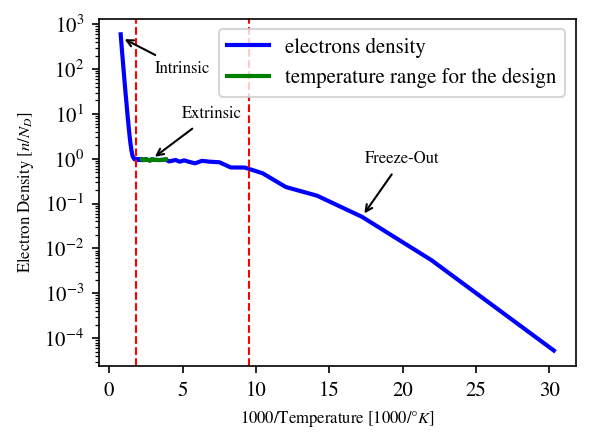
\includegraphics[width=0.6\textwidth]{carrier_density}
    %% Creator: Matplotlib, PGF backend
%%
%% To include the figure in your LaTeX document, write
%%   \input{<filename>.pgf}
%%
%% Make sure the required packages are loaded in your preamble
%%   \usepackage{pgf}
%%
%% Figures using additional raster images can only be included by \input if
%% they are in the same directory as the main LaTeX file. For loading figures
%% from other directories you can use the `import` package
%%   \usepackage{import}
%% and then include the figures with
%%   \import{<path to file>}{<filename>.pgf}
%%
%% Matplotlib used the following preamble
%%   \usepackage{gensymb}
%%   \usepackage[utf8x]{inputenc}
%%   \usepackage[T1]{fontenc}
%%
\begingroup%
\makeatletter%
\begin{pgfpicture}%
\pgfpathrectangle{\pgfpointorigin}{\pgfqpoint{3.930000in}{2.930000in}}%
\pgfusepath{use as bounding box, clip}%
\begin{pgfscope}%
\pgfsetbuttcap%
\pgfsetmiterjoin%
\definecolor{currentfill}{rgb}{1.000000,1.000000,1.000000}%
\pgfsetfillcolor{currentfill}%
\pgfsetlinewidth{0.000000pt}%
\definecolor{currentstroke}{rgb}{1.000000,1.000000,1.000000}%
\pgfsetstrokecolor{currentstroke}%
\pgfsetdash{}{0pt}%
\pgfpathmoveto{\pgfqpoint{0.000000in}{0.000000in}}%
\pgfpathlineto{\pgfqpoint{3.930000in}{0.000000in}}%
\pgfpathlineto{\pgfqpoint{3.930000in}{2.930000in}}%
\pgfpathlineto{\pgfqpoint{0.000000in}{2.930000in}}%
\pgfpathclose%
\pgfusepath{fill}%
\end{pgfscope}%
\begin{pgfscope}%
\pgfsetbuttcap%
\pgfsetmiterjoin%
\definecolor{currentfill}{rgb}{1.000000,1.000000,1.000000}%
\pgfsetfillcolor{currentfill}%
\pgfsetlinewidth{0.000000pt}%
\definecolor{currentstroke}{rgb}{0.000000,0.000000,0.000000}%
\pgfsetstrokecolor{currentstroke}%
\pgfsetstrokeopacity{0.000000}%
\pgfsetdash{}{0pt}%
\pgfpathmoveto{\pgfqpoint{0.665780in}{0.506466in}}%
\pgfpathlineto{\pgfqpoint{3.806667in}{0.506466in}}%
\pgfpathlineto{\pgfqpoint{3.806667in}{2.806667in}}%
\pgfpathlineto{\pgfqpoint{0.665780in}{2.806667in}}%
\pgfpathclose%
\pgfusepath{fill}%
\end{pgfscope}%
\begin{pgfscope}%
\pgfsetbuttcap%
\pgfsetroundjoin%
\definecolor{currentfill}{rgb}{0.000000,0.000000,0.000000}%
\pgfsetfillcolor{currentfill}%
\pgfsetlinewidth{0.803000pt}%
\definecolor{currentstroke}{rgb}{0.000000,0.000000,0.000000}%
\pgfsetstrokecolor{currentstroke}%
\pgfsetdash{}{0pt}%
\pgfsys@defobject{currentmarker}{\pgfqpoint{0.000000in}{-0.048611in}}{\pgfqpoint{0.000000in}{0.000000in}}{%
\pgfpathmoveto{\pgfqpoint{0.000000in}{0.000000in}}%
\pgfpathlineto{\pgfqpoint{0.000000in}{-0.048611in}}%
\pgfusepath{stroke,fill}%
}%
\begin{pgfscope}%
\pgfsys@transformshift{0.732559in}{0.506466in}%
\pgfsys@useobject{currentmarker}{}%
\end{pgfscope}%
\end{pgfscope}%
\begin{pgfscope}%
\pgftext[x=0.732559in,y=0.409244in,,top]{\fontsize{10.000000}{12.000000}\selectfont \(\displaystyle 0\)}%
\end{pgfscope}%
\begin{pgfscope}%
\pgfsetbuttcap%
\pgfsetroundjoin%
\definecolor{currentfill}{rgb}{0.000000,0.000000,0.000000}%
\pgfsetfillcolor{currentfill}%
\pgfsetlinewidth{0.803000pt}%
\definecolor{currentstroke}{rgb}{0.000000,0.000000,0.000000}%
\pgfsetstrokecolor{currentstroke}%
\pgfsetdash{}{0pt}%
\pgfsys@defobject{currentmarker}{\pgfqpoint{0.000000in}{-0.048611in}}{\pgfqpoint{0.000000in}{0.000000in}}{%
\pgfpathmoveto{\pgfqpoint{0.000000in}{0.000000in}}%
\pgfpathlineto{\pgfqpoint{0.000000in}{-0.048611in}}%
\pgfusepath{stroke,fill}%
}%
\begin{pgfscope}%
\pgfsys@transformshift{1.216230in}{0.506466in}%
\pgfsys@useobject{currentmarker}{}%
\end{pgfscope}%
\end{pgfscope}%
\begin{pgfscope}%
\pgftext[x=1.216230in,y=0.409244in,,top]{\fontsize{10.000000}{12.000000}\selectfont \(\displaystyle 5\)}%
\end{pgfscope}%
\begin{pgfscope}%
\pgfsetbuttcap%
\pgfsetroundjoin%
\definecolor{currentfill}{rgb}{0.000000,0.000000,0.000000}%
\pgfsetfillcolor{currentfill}%
\pgfsetlinewidth{0.803000pt}%
\definecolor{currentstroke}{rgb}{0.000000,0.000000,0.000000}%
\pgfsetstrokecolor{currentstroke}%
\pgfsetdash{}{0pt}%
\pgfsys@defobject{currentmarker}{\pgfqpoint{0.000000in}{-0.048611in}}{\pgfqpoint{0.000000in}{0.000000in}}{%
\pgfpathmoveto{\pgfqpoint{0.000000in}{0.000000in}}%
\pgfpathlineto{\pgfqpoint{0.000000in}{-0.048611in}}%
\pgfusepath{stroke,fill}%
}%
\begin{pgfscope}%
\pgfsys@transformshift{1.699901in}{0.506466in}%
\pgfsys@useobject{currentmarker}{}%
\end{pgfscope}%
\end{pgfscope}%
\begin{pgfscope}%
\pgftext[x=1.699901in,y=0.409244in,,top]{\fontsize{10.000000}{12.000000}\selectfont \(\displaystyle 10\)}%
\end{pgfscope}%
\begin{pgfscope}%
\pgfsetbuttcap%
\pgfsetroundjoin%
\definecolor{currentfill}{rgb}{0.000000,0.000000,0.000000}%
\pgfsetfillcolor{currentfill}%
\pgfsetlinewidth{0.803000pt}%
\definecolor{currentstroke}{rgb}{0.000000,0.000000,0.000000}%
\pgfsetstrokecolor{currentstroke}%
\pgfsetdash{}{0pt}%
\pgfsys@defobject{currentmarker}{\pgfqpoint{0.000000in}{-0.048611in}}{\pgfqpoint{0.000000in}{0.000000in}}{%
\pgfpathmoveto{\pgfqpoint{0.000000in}{0.000000in}}%
\pgfpathlineto{\pgfqpoint{0.000000in}{-0.048611in}}%
\pgfusepath{stroke,fill}%
}%
\begin{pgfscope}%
\pgfsys@transformshift{2.183572in}{0.506466in}%
\pgfsys@useobject{currentmarker}{}%
\end{pgfscope}%
\end{pgfscope}%
\begin{pgfscope}%
\pgftext[x=2.183572in,y=0.409244in,,top]{\fontsize{10.000000}{12.000000}\selectfont \(\displaystyle 15\)}%
\end{pgfscope}%
\begin{pgfscope}%
\pgfsetbuttcap%
\pgfsetroundjoin%
\definecolor{currentfill}{rgb}{0.000000,0.000000,0.000000}%
\pgfsetfillcolor{currentfill}%
\pgfsetlinewidth{0.803000pt}%
\definecolor{currentstroke}{rgb}{0.000000,0.000000,0.000000}%
\pgfsetstrokecolor{currentstroke}%
\pgfsetdash{}{0pt}%
\pgfsys@defobject{currentmarker}{\pgfqpoint{0.000000in}{-0.048611in}}{\pgfqpoint{0.000000in}{0.000000in}}{%
\pgfpathmoveto{\pgfqpoint{0.000000in}{0.000000in}}%
\pgfpathlineto{\pgfqpoint{0.000000in}{-0.048611in}}%
\pgfusepath{stroke,fill}%
}%
\begin{pgfscope}%
\pgfsys@transformshift{2.667243in}{0.506466in}%
\pgfsys@useobject{currentmarker}{}%
\end{pgfscope}%
\end{pgfscope}%
\begin{pgfscope}%
\pgftext[x=2.667243in,y=0.409244in,,top]{\fontsize{10.000000}{12.000000}\selectfont \(\displaystyle 20\)}%
\end{pgfscope}%
\begin{pgfscope}%
\pgfsetbuttcap%
\pgfsetroundjoin%
\definecolor{currentfill}{rgb}{0.000000,0.000000,0.000000}%
\pgfsetfillcolor{currentfill}%
\pgfsetlinewidth{0.803000pt}%
\definecolor{currentstroke}{rgb}{0.000000,0.000000,0.000000}%
\pgfsetstrokecolor{currentstroke}%
\pgfsetdash{}{0pt}%
\pgfsys@defobject{currentmarker}{\pgfqpoint{0.000000in}{-0.048611in}}{\pgfqpoint{0.000000in}{0.000000in}}{%
\pgfpathmoveto{\pgfqpoint{0.000000in}{0.000000in}}%
\pgfpathlineto{\pgfqpoint{0.000000in}{-0.048611in}}%
\pgfusepath{stroke,fill}%
}%
\begin{pgfscope}%
\pgfsys@transformshift{3.150915in}{0.506466in}%
\pgfsys@useobject{currentmarker}{}%
\end{pgfscope}%
\end{pgfscope}%
\begin{pgfscope}%
\pgftext[x=3.150915in,y=0.409244in,,top]{\fontsize{10.000000}{12.000000}\selectfont \(\displaystyle 25\)}%
\end{pgfscope}%
\begin{pgfscope}%
\pgfsetbuttcap%
\pgfsetroundjoin%
\definecolor{currentfill}{rgb}{0.000000,0.000000,0.000000}%
\pgfsetfillcolor{currentfill}%
\pgfsetlinewidth{0.803000pt}%
\definecolor{currentstroke}{rgb}{0.000000,0.000000,0.000000}%
\pgfsetstrokecolor{currentstroke}%
\pgfsetdash{}{0pt}%
\pgfsys@defobject{currentmarker}{\pgfqpoint{0.000000in}{-0.048611in}}{\pgfqpoint{0.000000in}{0.000000in}}{%
\pgfpathmoveto{\pgfqpoint{0.000000in}{0.000000in}}%
\pgfpathlineto{\pgfqpoint{0.000000in}{-0.048611in}}%
\pgfusepath{stroke,fill}%
}%
\begin{pgfscope}%
\pgfsys@transformshift{3.634586in}{0.506466in}%
\pgfsys@useobject{currentmarker}{}%
\end{pgfscope}%
\end{pgfscope}%
\begin{pgfscope}%
\pgftext[x=3.634586in,y=0.409244in,,top]{\fontsize{10.000000}{12.000000}\selectfont \(\displaystyle 30\)}%
\end{pgfscope}%
\begin{pgfscope}%
\pgftext[x=2.236223in,y=0.231033in,,top]{\fontsize{9.000000}{10.800000}\selectfont 1000/Temperature [\(\displaystyle 1000/K\)]}%
\end{pgfscope}%
\begin{pgfscope}%
\pgfsetbuttcap%
\pgfsetroundjoin%
\definecolor{currentfill}{rgb}{0.000000,0.000000,0.000000}%
\pgfsetfillcolor{currentfill}%
\pgfsetlinewidth{0.803000pt}%
\definecolor{currentstroke}{rgb}{0.000000,0.000000,0.000000}%
\pgfsetstrokecolor{currentstroke}%
\pgfsetdash{}{0pt}%
\pgfsys@defobject{currentmarker}{\pgfqpoint{-0.048611in}{0.000000in}}{\pgfqpoint{0.000000in}{0.000000in}}{%
\pgfpathmoveto{\pgfqpoint{0.000000in}{0.000000in}}%
\pgfpathlineto{\pgfqpoint{-0.048611in}{0.000000in}}%
\pgfusepath{stroke,fill}%
}%
\begin{pgfscope}%
\pgfsys@transformshift{0.665780in}{0.692513in}%
\pgfsys@useobject{currentmarker}{}%
\end{pgfscope}%
\end{pgfscope}%
\begin{pgfscope}%
\pgftext[x=0.280556in,y=0.644685in,left,base]{\fontsize{10.000000}{12.000000}\selectfont \(\displaystyle 10^{-4}\)}%
\end{pgfscope}%
\begin{pgfscope}%
\pgfsetbuttcap%
\pgfsetroundjoin%
\definecolor{currentfill}{rgb}{0.000000,0.000000,0.000000}%
\pgfsetfillcolor{currentfill}%
\pgfsetlinewidth{0.803000pt}%
\definecolor{currentstroke}{rgb}{0.000000,0.000000,0.000000}%
\pgfsetstrokecolor{currentstroke}%
\pgfsetdash{}{0pt}%
\pgfsys@defobject{currentmarker}{\pgfqpoint{-0.048611in}{0.000000in}}{\pgfqpoint{0.000000in}{0.000000in}}{%
\pgfpathmoveto{\pgfqpoint{0.000000in}{0.000000in}}%
\pgfpathlineto{\pgfqpoint{-0.048611in}{0.000000in}}%
\pgfusepath{stroke,fill}%
}%
\begin{pgfscope}%
\pgfsys@transformshift{0.665780in}{0.989098in}%
\pgfsys@useobject{currentmarker}{}%
\end{pgfscope}%
\end{pgfscope}%
\begin{pgfscope}%
\pgftext[x=0.280556in,y=0.941270in,left,base]{\fontsize{10.000000}{12.000000}\selectfont \(\displaystyle 10^{-3}\)}%
\end{pgfscope}%
\begin{pgfscope}%
\pgfsetbuttcap%
\pgfsetroundjoin%
\definecolor{currentfill}{rgb}{0.000000,0.000000,0.000000}%
\pgfsetfillcolor{currentfill}%
\pgfsetlinewidth{0.803000pt}%
\definecolor{currentstroke}{rgb}{0.000000,0.000000,0.000000}%
\pgfsetstrokecolor{currentstroke}%
\pgfsetdash{}{0pt}%
\pgfsys@defobject{currentmarker}{\pgfqpoint{-0.048611in}{0.000000in}}{\pgfqpoint{0.000000in}{0.000000in}}{%
\pgfpathmoveto{\pgfqpoint{0.000000in}{0.000000in}}%
\pgfpathlineto{\pgfqpoint{-0.048611in}{0.000000in}}%
\pgfusepath{stroke,fill}%
}%
\begin{pgfscope}%
\pgfsys@transformshift{0.665780in}{1.285683in}%
\pgfsys@useobject{currentmarker}{}%
\end{pgfscope}%
\end{pgfscope}%
\begin{pgfscope}%
\pgftext[x=0.280556in,y=1.237856in,left,base]{\fontsize{10.000000}{12.000000}\selectfont \(\displaystyle 10^{-2}\)}%
\end{pgfscope}%
\begin{pgfscope}%
\pgfsetbuttcap%
\pgfsetroundjoin%
\definecolor{currentfill}{rgb}{0.000000,0.000000,0.000000}%
\pgfsetfillcolor{currentfill}%
\pgfsetlinewidth{0.803000pt}%
\definecolor{currentstroke}{rgb}{0.000000,0.000000,0.000000}%
\pgfsetstrokecolor{currentstroke}%
\pgfsetdash{}{0pt}%
\pgfsys@defobject{currentmarker}{\pgfqpoint{-0.048611in}{0.000000in}}{\pgfqpoint{0.000000in}{0.000000in}}{%
\pgfpathmoveto{\pgfqpoint{0.000000in}{0.000000in}}%
\pgfpathlineto{\pgfqpoint{-0.048611in}{0.000000in}}%
\pgfusepath{stroke,fill}%
}%
\begin{pgfscope}%
\pgfsys@transformshift{0.665780in}{1.582268in}%
\pgfsys@useobject{currentmarker}{}%
\end{pgfscope}%
\end{pgfscope}%
\begin{pgfscope}%
\pgftext[x=0.280556in,y=1.534441in,left,base]{\fontsize{10.000000}{12.000000}\selectfont \(\displaystyle 10^{-1}\)}%
\end{pgfscope}%
\begin{pgfscope}%
\pgfsetbuttcap%
\pgfsetroundjoin%
\definecolor{currentfill}{rgb}{0.000000,0.000000,0.000000}%
\pgfsetfillcolor{currentfill}%
\pgfsetlinewidth{0.803000pt}%
\definecolor{currentstroke}{rgb}{0.000000,0.000000,0.000000}%
\pgfsetstrokecolor{currentstroke}%
\pgfsetdash{}{0pt}%
\pgfsys@defobject{currentmarker}{\pgfqpoint{-0.048611in}{0.000000in}}{\pgfqpoint{0.000000in}{0.000000in}}{%
\pgfpathmoveto{\pgfqpoint{0.000000in}{0.000000in}}%
\pgfpathlineto{\pgfqpoint{-0.048611in}{0.000000in}}%
\pgfusepath{stroke,fill}%
}%
\begin{pgfscope}%
\pgfsys@transformshift{0.665780in}{1.878853in}%
\pgfsys@useobject{currentmarker}{}%
\end{pgfscope}%
\end{pgfscope}%
\begin{pgfscope}%
\pgftext[x=0.367361in,y=1.831026in,left,base]{\fontsize{10.000000}{12.000000}\selectfont \(\displaystyle 10^{0}\)}%
\end{pgfscope}%
\begin{pgfscope}%
\pgfsetbuttcap%
\pgfsetroundjoin%
\definecolor{currentfill}{rgb}{0.000000,0.000000,0.000000}%
\pgfsetfillcolor{currentfill}%
\pgfsetlinewidth{0.803000pt}%
\definecolor{currentstroke}{rgb}{0.000000,0.000000,0.000000}%
\pgfsetstrokecolor{currentstroke}%
\pgfsetdash{}{0pt}%
\pgfsys@defobject{currentmarker}{\pgfqpoint{-0.048611in}{0.000000in}}{\pgfqpoint{0.000000in}{0.000000in}}{%
\pgfpathmoveto{\pgfqpoint{0.000000in}{0.000000in}}%
\pgfpathlineto{\pgfqpoint{-0.048611in}{0.000000in}}%
\pgfusepath{stroke,fill}%
}%
\begin{pgfscope}%
\pgfsys@transformshift{0.665780in}{2.175438in}%
\pgfsys@useobject{currentmarker}{}%
\end{pgfscope}%
\end{pgfscope}%
\begin{pgfscope}%
\pgftext[x=0.367361in,y=2.127611in,left,base]{\fontsize{10.000000}{12.000000}\selectfont \(\displaystyle 10^{1}\)}%
\end{pgfscope}%
\begin{pgfscope}%
\pgfsetbuttcap%
\pgfsetroundjoin%
\definecolor{currentfill}{rgb}{0.000000,0.000000,0.000000}%
\pgfsetfillcolor{currentfill}%
\pgfsetlinewidth{0.803000pt}%
\definecolor{currentstroke}{rgb}{0.000000,0.000000,0.000000}%
\pgfsetstrokecolor{currentstroke}%
\pgfsetdash{}{0pt}%
\pgfsys@defobject{currentmarker}{\pgfqpoint{-0.048611in}{0.000000in}}{\pgfqpoint{0.000000in}{0.000000in}}{%
\pgfpathmoveto{\pgfqpoint{0.000000in}{0.000000in}}%
\pgfpathlineto{\pgfqpoint{-0.048611in}{0.000000in}}%
\pgfusepath{stroke,fill}%
}%
\begin{pgfscope}%
\pgfsys@transformshift{0.665780in}{2.472024in}%
\pgfsys@useobject{currentmarker}{}%
\end{pgfscope}%
\end{pgfscope}%
\begin{pgfscope}%
\pgftext[x=0.367361in,y=2.424196in,left,base]{\fontsize{10.000000}{12.000000}\selectfont \(\displaystyle 10^{2}\)}%
\end{pgfscope}%
\begin{pgfscope}%
\pgfsetbuttcap%
\pgfsetroundjoin%
\definecolor{currentfill}{rgb}{0.000000,0.000000,0.000000}%
\pgfsetfillcolor{currentfill}%
\pgfsetlinewidth{0.803000pt}%
\definecolor{currentstroke}{rgb}{0.000000,0.000000,0.000000}%
\pgfsetstrokecolor{currentstroke}%
\pgfsetdash{}{0pt}%
\pgfsys@defobject{currentmarker}{\pgfqpoint{-0.048611in}{0.000000in}}{\pgfqpoint{0.000000in}{0.000000in}}{%
\pgfpathmoveto{\pgfqpoint{0.000000in}{0.000000in}}%
\pgfpathlineto{\pgfqpoint{-0.048611in}{0.000000in}}%
\pgfusepath{stroke,fill}%
}%
\begin{pgfscope}%
\pgfsys@transformshift{0.665780in}{2.768609in}%
\pgfsys@useobject{currentmarker}{}%
\end{pgfscope}%
\end{pgfscope}%
\begin{pgfscope}%
\pgftext[x=0.367361in,y=2.720781in,left,base]{\fontsize{10.000000}{12.000000}\selectfont \(\displaystyle 10^{3}\)}%
\end{pgfscope}%
\begin{pgfscope}%
\pgfsetbuttcap%
\pgfsetroundjoin%
\definecolor{currentfill}{rgb}{0.000000,0.000000,0.000000}%
\pgfsetfillcolor{currentfill}%
\pgfsetlinewidth{0.602250pt}%
\definecolor{currentstroke}{rgb}{0.000000,0.000000,0.000000}%
\pgfsetstrokecolor{currentstroke}%
\pgfsetdash{}{0pt}%
\pgfsys@defobject{currentmarker}{\pgfqpoint{-0.027778in}{0.000000in}}{\pgfqpoint{0.000000in}{0.000000in}}{%
\pgfpathmoveto{\pgfqpoint{0.000000in}{0.000000in}}%
\pgfpathlineto{\pgfqpoint{-0.027778in}{0.000000in}}%
\pgfusepath{stroke,fill}%
}%
\begin{pgfscope}%
\pgfsys@transformshift{0.665780in}{0.537435in}%
\pgfsys@useobject{currentmarker}{}%
\end{pgfscope}%
\end{pgfscope}%
\begin{pgfscope}%
\pgfsetbuttcap%
\pgfsetroundjoin%
\definecolor{currentfill}{rgb}{0.000000,0.000000,0.000000}%
\pgfsetfillcolor{currentfill}%
\pgfsetlinewidth{0.602250pt}%
\definecolor{currentstroke}{rgb}{0.000000,0.000000,0.000000}%
\pgfsetstrokecolor{currentstroke}%
\pgfsetdash{}{0pt}%
\pgfsys@defobject{currentmarker}{\pgfqpoint{-0.027778in}{0.000000in}}{\pgfqpoint{0.000000in}{0.000000in}}{%
\pgfpathmoveto{\pgfqpoint{0.000000in}{0.000000in}}%
\pgfpathlineto{\pgfqpoint{-0.027778in}{0.000000in}}%
\pgfusepath{stroke,fill}%
}%
\begin{pgfscope}%
\pgfsys@transformshift{0.665780in}{0.574490in}%
\pgfsys@useobject{currentmarker}{}%
\end{pgfscope}%
\end{pgfscope}%
\begin{pgfscope}%
\pgfsetbuttcap%
\pgfsetroundjoin%
\definecolor{currentfill}{rgb}{0.000000,0.000000,0.000000}%
\pgfsetfillcolor{currentfill}%
\pgfsetlinewidth{0.602250pt}%
\definecolor{currentstroke}{rgb}{0.000000,0.000000,0.000000}%
\pgfsetstrokecolor{currentstroke}%
\pgfsetdash{}{0pt}%
\pgfsys@defobject{currentmarker}{\pgfqpoint{-0.027778in}{0.000000in}}{\pgfqpoint{0.000000in}{0.000000in}}{%
\pgfpathmoveto{\pgfqpoint{0.000000in}{0.000000in}}%
\pgfpathlineto{\pgfqpoint{-0.027778in}{0.000000in}}%
\pgfusepath{stroke,fill}%
}%
\begin{pgfscope}%
\pgfsys@transformshift{0.665780in}{0.603232in}%
\pgfsys@useobject{currentmarker}{}%
\end{pgfscope}%
\end{pgfscope}%
\begin{pgfscope}%
\pgfsetbuttcap%
\pgfsetroundjoin%
\definecolor{currentfill}{rgb}{0.000000,0.000000,0.000000}%
\pgfsetfillcolor{currentfill}%
\pgfsetlinewidth{0.602250pt}%
\definecolor{currentstroke}{rgb}{0.000000,0.000000,0.000000}%
\pgfsetstrokecolor{currentstroke}%
\pgfsetdash{}{0pt}%
\pgfsys@defobject{currentmarker}{\pgfqpoint{-0.027778in}{0.000000in}}{\pgfqpoint{0.000000in}{0.000000in}}{%
\pgfpathmoveto{\pgfqpoint{0.000000in}{0.000000in}}%
\pgfpathlineto{\pgfqpoint{-0.027778in}{0.000000in}}%
\pgfusepath{stroke,fill}%
}%
\begin{pgfscope}%
\pgfsys@transformshift{0.665780in}{0.626716in}%
\pgfsys@useobject{currentmarker}{}%
\end{pgfscope}%
\end{pgfscope}%
\begin{pgfscope}%
\pgfsetbuttcap%
\pgfsetroundjoin%
\definecolor{currentfill}{rgb}{0.000000,0.000000,0.000000}%
\pgfsetfillcolor{currentfill}%
\pgfsetlinewidth{0.602250pt}%
\definecolor{currentstroke}{rgb}{0.000000,0.000000,0.000000}%
\pgfsetstrokecolor{currentstroke}%
\pgfsetdash{}{0pt}%
\pgfsys@defobject{currentmarker}{\pgfqpoint{-0.027778in}{0.000000in}}{\pgfqpoint{0.000000in}{0.000000in}}{%
\pgfpathmoveto{\pgfqpoint{0.000000in}{0.000000in}}%
\pgfpathlineto{\pgfqpoint{-0.027778in}{0.000000in}}%
\pgfusepath{stroke,fill}%
}%
\begin{pgfscope}%
\pgfsys@transformshift{0.665780in}{0.646572in}%
\pgfsys@useobject{currentmarker}{}%
\end{pgfscope}%
\end{pgfscope}%
\begin{pgfscope}%
\pgfsetbuttcap%
\pgfsetroundjoin%
\definecolor{currentfill}{rgb}{0.000000,0.000000,0.000000}%
\pgfsetfillcolor{currentfill}%
\pgfsetlinewidth{0.602250pt}%
\definecolor{currentstroke}{rgb}{0.000000,0.000000,0.000000}%
\pgfsetstrokecolor{currentstroke}%
\pgfsetdash{}{0pt}%
\pgfsys@defobject{currentmarker}{\pgfqpoint{-0.027778in}{0.000000in}}{\pgfqpoint{0.000000in}{0.000000in}}{%
\pgfpathmoveto{\pgfqpoint{0.000000in}{0.000000in}}%
\pgfpathlineto{\pgfqpoint{-0.027778in}{0.000000in}}%
\pgfusepath{stroke,fill}%
}%
\begin{pgfscope}%
\pgfsys@transformshift{0.665780in}{0.663771in}%
\pgfsys@useobject{currentmarker}{}%
\end{pgfscope}%
\end{pgfscope}%
\begin{pgfscope}%
\pgfsetbuttcap%
\pgfsetroundjoin%
\definecolor{currentfill}{rgb}{0.000000,0.000000,0.000000}%
\pgfsetfillcolor{currentfill}%
\pgfsetlinewidth{0.602250pt}%
\definecolor{currentstroke}{rgb}{0.000000,0.000000,0.000000}%
\pgfsetstrokecolor{currentstroke}%
\pgfsetdash{}{0pt}%
\pgfsys@defobject{currentmarker}{\pgfqpoint{-0.027778in}{0.000000in}}{\pgfqpoint{0.000000in}{0.000000in}}{%
\pgfpathmoveto{\pgfqpoint{0.000000in}{0.000000in}}%
\pgfpathlineto{\pgfqpoint{-0.027778in}{0.000000in}}%
\pgfusepath{stroke,fill}%
}%
\begin{pgfscope}%
\pgfsys@transformshift{0.665780in}{0.678942in}%
\pgfsys@useobject{currentmarker}{}%
\end{pgfscope}%
\end{pgfscope}%
\begin{pgfscope}%
\pgfsetbuttcap%
\pgfsetroundjoin%
\definecolor{currentfill}{rgb}{0.000000,0.000000,0.000000}%
\pgfsetfillcolor{currentfill}%
\pgfsetlinewidth{0.602250pt}%
\definecolor{currentstroke}{rgb}{0.000000,0.000000,0.000000}%
\pgfsetstrokecolor{currentstroke}%
\pgfsetdash{}{0pt}%
\pgfsys@defobject{currentmarker}{\pgfqpoint{-0.027778in}{0.000000in}}{\pgfqpoint{0.000000in}{0.000000in}}{%
\pgfpathmoveto{\pgfqpoint{0.000000in}{0.000000in}}%
\pgfpathlineto{\pgfqpoint{-0.027778in}{0.000000in}}%
\pgfusepath{stroke,fill}%
}%
\begin{pgfscope}%
\pgfsys@transformshift{0.665780in}{0.781794in}%
\pgfsys@useobject{currentmarker}{}%
\end{pgfscope}%
\end{pgfscope}%
\begin{pgfscope}%
\pgfsetbuttcap%
\pgfsetroundjoin%
\definecolor{currentfill}{rgb}{0.000000,0.000000,0.000000}%
\pgfsetfillcolor{currentfill}%
\pgfsetlinewidth{0.602250pt}%
\definecolor{currentstroke}{rgb}{0.000000,0.000000,0.000000}%
\pgfsetstrokecolor{currentstroke}%
\pgfsetdash{}{0pt}%
\pgfsys@defobject{currentmarker}{\pgfqpoint{-0.027778in}{0.000000in}}{\pgfqpoint{0.000000in}{0.000000in}}{%
\pgfpathmoveto{\pgfqpoint{0.000000in}{0.000000in}}%
\pgfpathlineto{\pgfqpoint{-0.027778in}{0.000000in}}%
\pgfusepath{stroke,fill}%
}%
\begin{pgfscope}%
\pgfsys@transformshift{0.665780in}{0.834020in}%
\pgfsys@useobject{currentmarker}{}%
\end{pgfscope}%
\end{pgfscope}%
\begin{pgfscope}%
\pgfsetbuttcap%
\pgfsetroundjoin%
\definecolor{currentfill}{rgb}{0.000000,0.000000,0.000000}%
\pgfsetfillcolor{currentfill}%
\pgfsetlinewidth{0.602250pt}%
\definecolor{currentstroke}{rgb}{0.000000,0.000000,0.000000}%
\pgfsetstrokecolor{currentstroke}%
\pgfsetdash{}{0pt}%
\pgfsys@defobject{currentmarker}{\pgfqpoint{-0.027778in}{0.000000in}}{\pgfqpoint{0.000000in}{0.000000in}}{%
\pgfpathmoveto{\pgfqpoint{0.000000in}{0.000000in}}%
\pgfpathlineto{\pgfqpoint{-0.027778in}{0.000000in}}%
\pgfusepath{stroke,fill}%
}%
\begin{pgfscope}%
\pgfsys@transformshift{0.665780in}{0.871075in}%
\pgfsys@useobject{currentmarker}{}%
\end{pgfscope}%
\end{pgfscope}%
\begin{pgfscope}%
\pgfsetbuttcap%
\pgfsetroundjoin%
\definecolor{currentfill}{rgb}{0.000000,0.000000,0.000000}%
\pgfsetfillcolor{currentfill}%
\pgfsetlinewidth{0.602250pt}%
\definecolor{currentstroke}{rgb}{0.000000,0.000000,0.000000}%
\pgfsetstrokecolor{currentstroke}%
\pgfsetdash{}{0pt}%
\pgfsys@defobject{currentmarker}{\pgfqpoint{-0.027778in}{0.000000in}}{\pgfqpoint{0.000000in}{0.000000in}}{%
\pgfpathmoveto{\pgfqpoint{0.000000in}{0.000000in}}%
\pgfpathlineto{\pgfqpoint{-0.027778in}{0.000000in}}%
\pgfusepath{stroke,fill}%
}%
\begin{pgfscope}%
\pgfsys@transformshift{0.665780in}{0.899817in}%
\pgfsys@useobject{currentmarker}{}%
\end{pgfscope}%
\end{pgfscope}%
\begin{pgfscope}%
\pgfsetbuttcap%
\pgfsetroundjoin%
\definecolor{currentfill}{rgb}{0.000000,0.000000,0.000000}%
\pgfsetfillcolor{currentfill}%
\pgfsetlinewidth{0.602250pt}%
\definecolor{currentstroke}{rgb}{0.000000,0.000000,0.000000}%
\pgfsetstrokecolor{currentstroke}%
\pgfsetdash{}{0pt}%
\pgfsys@defobject{currentmarker}{\pgfqpoint{-0.027778in}{0.000000in}}{\pgfqpoint{0.000000in}{0.000000in}}{%
\pgfpathmoveto{\pgfqpoint{0.000000in}{0.000000in}}%
\pgfpathlineto{\pgfqpoint{-0.027778in}{0.000000in}}%
\pgfusepath{stroke,fill}%
}%
\begin{pgfscope}%
\pgfsys@transformshift{0.665780in}{0.923301in}%
\pgfsys@useobject{currentmarker}{}%
\end{pgfscope}%
\end{pgfscope}%
\begin{pgfscope}%
\pgfsetbuttcap%
\pgfsetroundjoin%
\definecolor{currentfill}{rgb}{0.000000,0.000000,0.000000}%
\pgfsetfillcolor{currentfill}%
\pgfsetlinewidth{0.602250pt}%
\definecolor{currentstroke}{rgb}{0.000000,0.000000,0.000000}%
\pgfsetstrokecolor{currentstroke}%
\pgfsetdash{}{0pt}%
\pgfsys@defobject{currentmarker}{\pgfqpoint{-0.027778in}{0.000000in}}{\pgfqpoint{0.000000in}{0.000000in}}{%
\pgfpathmoveto{\pgfqpoint{0.000000in}{0.000000in}}%
\pgfpathlineto{\pgfqpoint{-0.027778in}{0.000000in}}%
\pgfusepath{stroke,fill}%
}%
\begin{pgfscope}%
\pgfsys@transformshift{0.665780in}{0.943157in}%
\pgfsys@useobject{currentmarker}{}%
\end{pgfscope}%
\end{pgfscope}%
\begin{pgfscope}%
\pgfsetbuttcap%
\pgfsetroundjoin%
\definecolor{currentfill}{rgb}{0.000000,0.000000,0.000000}%
\pgfsetfillcolor{currentfill}%
\pgfsetlinewidth{0.602250pt}%
\definecolor{currentstroke}{rgb}{0.000000,0.000000,0.000000}%
\pgfsetstrokecolor{currentstroke}%
\pgfsetdash{}{0pt}%
\pgfsys@defobject{currentmarker}{\pgfqpoint{-0.027778in}{0.000000in}}{\pgfqpoint{0.000000in}{0.000000in}}{%
\pgfpathmoveto{\pgfqpoint{0.000000in}{0.000000in}}%
\pgfpathlineto{\pgfqpoint{-0.027778in}{0.000000in}}%
\pgfusepath{stroke,fill}%
}%
\begin{pgfscope}%
\pgfsys@transformshift{0.665780in}{0.960356in}%
\pgfsys@useobject{currentmarker}{}%
\end{pgfscope}%
\end{pgfscope}%
\begin{pgfscope}%
\pgfsetbuttcap%
\pgfsetroundjoin%
\definecolor{currentfill}{rgb}{0.000000,0.000000,0.000000}%
\pgfsetfillcolor{currentfill}%
\pgfsetlinewidth{0.602250pt}%
\definecolor{currentstroke}{rgb}{0.000000,0.000000,0.000000}%
\pgfsetstrokecolor{currentstroke}%
\pgfsetdash{}{0pt}%
\pgfsys@defobject{currentmarker}{\pgfqpoint{-0.027778in}{0.000000in}}{\pgfqpoint{0.000000in}{0.000000in}}{%
\pgfpathmoveto{\pgfqpoint{0.000000in}{0.000000in}}%
\pgfpathlineto{\pgfqpoint{-0.027778in}{0.000000in}}%
\pgfusepath{stroke,fill}%
}%
\begin{pgfscope}%
\pgfsys@transformshift{0.665780in}{0.975527in}%
\pgfsys@useobject{currentmarker}{}%
\end{pgfscope}%
\end{pgfscope}%
\begin{pgfscope}%
\pgfsetbuttcap%
\pgfsetroundjoin%
\definecolor{currentfill}{rgb}{0.000000,0.000000,0.000000}%
\pgfsetfillcolor{currentfill}%
\pgfsetlinewidth{0.602250pt}%
\definecolor{currentstroke}{rgb}{0.000000,0.000000,0.000000}%
\pgfsetstrokecolor{currentstroke}%
\pgfsetdash{}{0pt}%
\pgfsys@defobject{currentmarker}{\pgfqpoint{-0.027778in}{0.000000in}}{\pgfqpoint{0.000000in}{0.000000in}}{%
\pgfpathmoveto{\pgfqpoint{0.000000in}{0.000000in}}%
\pgfpathlineto{\pgfqpoint{-0.027778in}{0.000000in}}%
\pgfusepath{stroke,fill}%
}%
\begin{pgfscope}%
\pgfsys@transformshift{0.665780in}{1.078379in}%
\pgfsys@useobject{currentmarker}{}%
\end{pgfscope}%
\end{pgfscope}%
\begin{pgfscope}%
\pgfsetbuttcap%
\pgfsetroundjoin%
\definecolor{currentfill}{rgb}{0.000000,0.000000,0.000000}%
\pgfsetfillcolor{currentfill}%
\pgfsetlinewidth{0.602250pt}%
\definecolor{currentstroke}{rgb}{0.000000,0.000000,0.000000}%
\pgfsetstrokecolor{currentstroke}%
\pgfsetdash{}{0pt}%
\pgfsys@defobject{currentmarker}{\pgfqpoint{-0.027778in}{0.000000in}}{\pgfqpoint{0.000000in}{0.000000in}}{%
\pgfpathmoveto{\pgfqpoint{0.000000in}{0.000000in}}%
\pgfpathlineto{\pgfqpoint{-0.027778in}{0.000000in}}%
\pgfusepath{stroke,fill}%
}%
\begin{pgfscope}%
\pgfsys@transformshift{0.665780in}{1.130605in}%
\pgfsys@useobject{currentmarker}{}%
\end{pgfscope}%
\end{pgfscope}%
\begin{pgfscope}%
\pgfsetbuttcap%
\pgfsetroundjoin%
\definecolor{currentfill}{rgb}{0.000000,0.000000,0.000000}%
\pgfsetfillcolor{currentfill}%
\pgfsetlinewidth{0.602250pt}%
\definecolor{currentstroke}{rgb}{0.000000,0.000000,0.000000}%
\pgfsetstrokecolor{currentstroke}%
\pgfsetdash{}{0pt}%
\pgfsys@defobject{currentmarker}{\pgfqpoint{-0.027778in}{0.000000in}}{\pgfqpoint{0.000000in}{0.000000in}}{%
\pgfpathmoveto{\pgfqpoint{0.000000in}{0.000000in}}%
\pgfpathlineto{\pgfqpoint{-0.027778in}{0.000000in}}%
\pgfusepath{stroke,fill}%
}%
\begin{pgfscope}%
\pgfsys@transformshift{0.665780in}{1.167660in}%
\pgfsys@useobject{currentmarker}{}%
\end{pgfscope}%
\end{pgfscope}%
\begin{pgfscope}%
\pgfsetbuttcap%
\pgfsetroundjoin%
\definecolor{currentfill}{rgb}{0.000000,0.000000,0.000000}%
\pgfsetfillcolor{currentfill}%
\pgfsetlinewidth{0.602250pt}%
\definecolor{currentstroke}{rgb}{0.000000,0.000000,0.000000}%
\pgfsetstrokecolor{currentstroke}%
\pgfsetdash{}{0pt}%
\pgfsys@defobject{currentmarker}{\pgfqpoint{-0.027778in}{0.000000in}}{\pgfqpoint{0.000000in}{0.000000in}}{%
\pgfpathmoveto{\pgfqpoint{0.000000in}{0.000000in}}%
\pgfpathlineto{\pgfqpoint{-0.027778in}{0.000000in}}%
\pgfusepath{stroke,fill}%
}%
\begin{pgfscope}%
\pgfsys@transformshift{0.665780in}{1.196402in}%
\pgfsys@useobject{currentmarker}{}%
\end{pgfscope}%
\end{pgfscope}%
\begin{pgfscope}%
\pgfsetbuttcap%
\pgfsetroundjoin%
\definecolor{currentfill}{rgb}{0.000000,0.000000,0.000000}%
\pgfsetfillcolor{currentfill}%
\pgfsetlinewidth{0.602250pt}%
\definecolor{currentstroke}{rgb}{0.000000,0.000000,0.000000}%
\pgfsetstrokecolor{currentstroke}%
\pgfsetdash{}{0pt}%
\pgfsys@defobject{currentmarker}{\pgfqpoint{-0.027778in}{0.000000in}}{\pgfqpoint{0.000000in}{0.000000in}}{%
\pgfpathmoveto{\pgfqpoint{0.000000in}{0.000000in}}%
\pgfpathlineto{\pgfqpoint{-0.027778in}{0.000000in}}%
\pgfusepath{stroke,fill}%
}%
\begin{pgfscope}%
\pgfsys@transformshift{0.665780in}{1.219886in}%
\pgfsys@useobject{currentmarker}{}%
\end{pgfscope}%
\end{pgfscope}%
\begin{pgfscope}%
\pgfsetbuttcap%
\pgfsetroundjoin%
\definecolor{currentfill}{rgb}{0.000000,0.000000,0.000000}%
\pgfsetfillcolor{currentfill}%
\pgfsetlinewidth{0.602250pt}%
\definecolor{currentstroke}{rgb}{0.000000,0.000000,0.000000}%
\pgfsetstrokecolor{currentstroke}%
\pgfsetdash{}{0pt}%
\pgfsys@defobject{currentmarker}{\pgfqpoint{-0.027778in}{0.000000in}}{\pgfqpoint{0.000000in}{0.000000in}}{%
\pgfpathmoveto{\pgfqpoint{0.000000in}{0.000000in}}%
\pgfpathlineto{\pgfqpoint{-0.027778in}{0.000000in}}%
\pgfusepath{stroke,fill}%
}%
\begin{pgfscope}%
\pgfsys@transformshift{0.665780in}{1.239742in}%
\pgfsys@useobject{currentmarker}{}%
\end{pgfscope}%
\end{pgfscope}%
\begin{pgfscope}%
\pgfsetbuttcap%
\pgfsetroundjoin%
\definecolor{currentfill}{rgb}{0.000000,0.000000,0.000000}%
\pgfsetfillcolor{currentfill}%
\pgfsetlinewidth{0.602250pt}%
\definecolor{currentstroke}{rgb}{0.000000,0.000000,0.000000}%
\pgfsetstrokecolor{currentstroke}%
\pgfsetdash{}{0pt}%
\pgfsys@defobject{currentmarker}{\pgfqpoint{-0.027778in}{0.000000in}}{\pgfqpoint{0.000000in}{0.000000in}}{%
\pgfpathmoveto{\pgfqpoint{0.000000in}{0.000000in}}%
\pgfpathlineto{\pgfqpoint{-0.027778in}{0.000000in}}%
\pgfusepath{stroke,fill}%
}%
\begin{pgfscope}%
\pgfsys@transformshift{0.665780in}{1.256941in}%
\pgfsys@useobject{currentmarker}{}%
\end{pgfscope}%
\end{pgfscope}%
\begin{pgfscope}%
\pgfsetbuttcap%
\pgfsetroundjoin%
\definecolor{currentfill}{rgb}{0.000000,0.000000,0.000000}%
\pgfsetfillcolor{currentfill}%
\pgfsetlinewidth{0.602250pt}%
\definecolor{currentstroke}{rgb}{0.000000,0.000000,0.000000}%
\pgfsetstrokecolor{currentstroke}%
\pgfsetdash{}{0pt}%
\pgfsys@defobject{currentmarker}{\pgfqpoint{-0.027778in}{0.000000in}}{\pgfqpoint{0.000000in}{0.000000in}}{%
\pgfpathmoveto{\pgfqpoint{0.000000in}{0.000000in}}%
\pgfpathlineto{\pgfqpoint{-0.027778in}{0.000000in}}%
\pgfusepath{stroke,fill}%
}%
\begin{pgfscope}%
\pgfsys@transformshift{0.665780in}{1.272112in}%
\pgfsys@useobject{currentmarker}{}%
\end{pgfscope}%
\end{pgfscope}%
\begin{pgfscope}%
\pgfsetbuttcap%
\pgfsetroundjoin%
\definecolor{currentfill}{rgb}{0.000000,0.000000,0.000000}%
\pgfsetfillcolor{currentfill}%
\pgfsetlinewidth{0.602250pt}%
\definecolor{currentstroke}{rgb}{0.000000,0.000000,0.000000}%
\pgfsetstrokecolor{currentstroke}%
\pgfsetdash{}{0pt}%
\pgfsys@defobject{currentmarker}{\pgfqpoint{-0.027778in}{0.000000in}}{\pgfqpoint{0.000000in}{0.000000in}}{%
\pgfpathmoveto{\pgfqpoint{0.000000in}{0.000000in}}%
\pgfpathlineto{\pgfqpoint{-0.027778in}{0.000000in}}%
\pgfusepath{stroke,fill}%
}%
\begin{pgfscope}%
\pgfsys@transformshift{0.665780in}{1.374964in}%
\pgfsys@useobject{currentmarker}{}%
\end{pgfscope}%
\end{pgfscope}%
\begin{pgfscope}%
\pgfsetbuttcap%
\pgfsetroundjoin%
\definecolor{currentfill}{rgb}{0.000000,0.000000,0.000000}%
\pgfsetfillcolor{currentfill}%
\pgfsetlinewidth{0.602250pt}%
\definecolor{currentstroke}{rgb}{0.000000,0.000000,0.000000}%
\pgfsetstrokecolor{currentstroke}%
\pgfsetdash{}{0pt}%
\pgfsys@defobject{currentmarker}{\pgfqpoint{-0.027778in}{0.000000in}}{\pgfqpoint{0.000000in}{0.000000in}}{%
\pgfpathmoveto{\pgfqpoint{0.000000in}{0.000000in}}%
\pgfpathlineto{\pgfqpoint{-0.027778in}{0.000000in}}%
\pgfusepath{stroke,fill}%
}%
\begin{pgfscope}%
\pgfsys@transformshift{0.665780in}{1.427190in}%
\pgfsys@useobject{currentmarker}{}%
\end{pgfscope}%
\end{pgfscope}%
\begin{pgfscope}%
\pgfsetbuttcap%
\pgfsetroundjoin%
\definecolor{currentfill}{rgb}{0.000000,0.000000,0.000000}%
\pgfsetfillcolor{currentfill}%
\pgfsetlinewidth{0.602250pt}%
\definecolor{currentstroke}{rgb}{0.000000,0.000000,0.000000}%
\pgfsetstrokecolor{currentstroke}%
\pgfsetdash{}{0pt}%
\pgfsys@defobject{currentmarker}{\pgfqpoint{-0.027778in}{0.000000in}}{\pgfqpoint{0.000000in}{0.000000in}}{%
\pgfpathmoveto{\pgfqpoint{0.000000in}{0.000000in}}%
\pgfpathlineto{\pgfqpoint{-0.027778in}{0.000000in}}%
\pgfusepath{stroke,fill}%
}%
\begin{pgfscope}%
\pgfsys@transformshift{0.665780in}{1.464245in}%
\pgfsys@useobject{currentmarker}{}%
\end{pgfscope}%
\end{pgfscope}%
\begin{pgfscope}%
\pgfsetbuttcap%
\pgfsetroundjoin%
\definecolor{currentfill}{rgb}{0.000000,0.000000,0.000000}%
\pgfsetfillcolor{currentfill}%
\pgfsetlinewidth{0.602250pt}%
\definecolor{currentstroke}{rgb}{0.000000,0.000000,0.000000}%
\pgfsetstrokecolor{currentstroke}%
\pgfsetdash{}{0pt}%
\pgfsys@defobject{currentmarker}{\pgfqpoint{-0.027778in}{0.000000in}}{\pgfqpoint{0.000000in}{0.000000in}}{%
\pgfpathmoveto{\pgfqpoint{0.000000in}{0.000000in}}%
\pgfpathlineto{\pgfqpoint{-0.027778in}{0.000000in}}%
\pgfusepath{stroke,fill}%
}%
\begin{pgfscope}%
\pgfsys@transformshift{0.665780in}{1.492987in}%
\pgfsys@useobject{currentmarker}{}%
\end{pgfscope}%
\end{pgfscope}%
\begin{pgfscope}%
\pgfsetbuttcap%
\pgfsetroundjoin%
\definecolor{currentfill}{rgb}{0.000000,0.000000,0.000000}%
\pgfsetfillcolor{currentfill}%
\pgfsetlinewidth{0.602250pt}%
\definecolor{currentstroke}{rgb}{0.000000,0.000000,0.000000}%
\pgfsetstrokecolor{currentstroke}%
\pgfsetdash{}{0pt}%
\pgfsys@defobject{currentmarker}{\pgfqpoint{-0.027778in}{0.000000in}}{\pgfqpoint{0.000000in}{0.000000in}}{%
\pgfpathmoveto{\pgfqpoint{0.000000in}{0.000000in}}%
\pgfpathlineto{\pgfqpoint{-0.027778in}{0.000000in}}%
\pgfusepath{stroke,fill}%
}%
\begin{pgfscope}%
\pgfsys@transformshift{0.665780in}{1.516471in}%
\pgfsys@useobject{currentmarker}{}%
\end{pgfscope}%
\end{pgfscope}%
\begin{pgfscope}%
\pgfsetbuttcap%
\pgfsetroundjoin%
\definecolor{currentfill}{rgb}{0.000000,0.000000,0.000000}%
\pgfsetfillcolor{currentfill}%
\pgfsetlinewidth{0.602250pt}%
\definecolor{currentstroke}{rgb}{0.000000,0.000000,0.000000}%
\pgfsetstrokecolor{currentstroke}%
\pgfsetdash{}{0pt}%
\pgfsys@defobject{currentmarker}{\pgfqpoint{-0.027778in}{0.000000in}}{\pgfqpoint{0.000000in}{0.000000in}}{%
\pgfpathmoveto{\pgfqpoint{0.000000in}{0.000000in}}%
\pgfpathlineto{\pgfqpoint{-0.027778in}{0.000000in}}%
\pgfusepath{stroke,fill}%
}%
\begin{pgfscope}%
\pgfsys@transformshift{0.665780in}{1.536327in}%
\pgfsys@useobject{currentmarker}{}%
\end{pgfscope}%
\end{pgfscope}%
\begin{pgfscope}%
\pgfsetbuttcap%
\pgfsetroundjoin%
\definecolor{currentfill}{rgb}{0.000000,0.000000,0.000000}%
\pgfsetfillcolor{currentfill}%
\pgfsetlinewidth{0.602250pt}%
\definecolor{currentstroke}{rgb}{0.000000,0.000000,0.000000}%
\pgfsetstrokecolor{currentstroke}%
\pgfsetdash{}{0pt}%
\pgfsys@defobject{currentmarker}{\pgfqpoint{-0.027778in}{0.000000in}}{\pgfqpoint{0.000000in}{0.000000in}}{%
\pgfpathmoveto{\pgfqpoint{0.000000in}{0.000000in}}%
\pgfpathlineto{\pgfqpoint{-0.027778in}{0.000000in}}%
\pgfusepath{stroke,fill}%
}%
\begin{pgfscope}%
\pgfsys@transformshift{0.665780in}{1.553526in}%
\pgfsys@useobject{currentmarker}{}%
\end{pgfscope}%
\end{pgfscope}%
\begin{pgfscope}%
\pgfsetbuttcap%
\pgfsetroundjoin%
\definecolor{currentfill}{rgb}{0.000000,0.000000,0.000000}%
\pgfsetfillcolor{currentfill}%
\pgfsetlinewidth{0.602250pt}%
\definecolor{currentstroke}{rgb}{0.000000,0.000000,0.000000}%
\pgfsetstrokecolor{currentstroke}%
\pgfsetdash{}{0pt}%
\pgfsys@defobject{currentmarker}{\pgfqpoint{-0.027778in}{0.000000in}}{\pgfqpoint{0.000000in}{0.000000in}}{%
\pgfpathmoveto{\pgfqpoint{0.000000in}{0.000000in}}%
\pgfpathlineto{\pgfqpoint{-0.027778in}{0.000000in}}%
\pgfusepath{stroke,fill}%
}%
\begin{pgfscope}%
\pgfsys@transformshift{0.665780in}{1.568697in}%
\pgfsys@useobject{currentmarker}{}%
\end{pgfscope}%
\end{pgfscope}%
\begin{pgfscope}%
\pgfsetbuttcap%
\pgfsetroundjoin%
\definecolor{currentfill}{rgb}{0.000000,0.000000,0.000000}%
\pgfsetfillcolor{currentfill}%
\pgfsetlinewidth{0.602250pt}%
\definecolor{currentstroke}{rgb}{0.000000,0.000000,0.000000}%
\pgfsetstrokecolor{currentstroke}%
\pgfsetdash{}{0pt}%
\pgfsys@defobject{currentmarker}{\pgfqpoint{-0.027778in}{0.000000in}}{\pgfqpoint{0.000000in}{0.000000in}}{%
\pgfpathmoveto{\pgfqpoint{0.000000in}{0.000000in}}%
\pgfpathlineto{\pgfqpoint{-0.027778in}{0.000000in}}%
\pgfusepath{stroke,fill}%
}%
\begin{pgfscope}%
\pgfsys@transformshift{0.665780in}{1.671549in}%
\pgfsys@useobject{currentmarker}{}%
\end{pgfscope}%
\end{pgfscope}%
\begin{pgfscope}%
\pgfsetbuttcap%
\pgfsetroundjoin%
\definecolor{currentfill}{rgb}{0.000000,0.000000,0.000000}%
\pgfsetfillcolor{currentfill}%
\pgfsetlinewidth{0.602250pt}%
\definecolor{currentstroke}{rgb}{0.000000,0.000000,0.000000}%
\pgfsetstrokecolor{currentstroke}%
\pgfsetdash{}{0pt}%
\pgfsys@defobject{currentmarker}{\pgfqpoint{-0.027778in}{0.000000in}}{\pgfqpoint{0.000000in}{0.000000in}}{%
\pgfpathmoveto{\pgfqpoint{0.000000in}{0.000000in}}%
\pgfpathlineto{\pgfqpoint{-0.027778in}{0.000000in}}%
\pgfusepath{stroke,fill}%
}%
\begin{pgfscope}%
\pgfsys@transformshift{0.665780in}{1.723775in}%
\pgfsys@useobject{currentmarker}{}%
\end{pgfscope}%
\end{pgfscope}%
\begin{pgfscope}%
\pgfsetbuttcap%
\pgfsetroundjoin%
\definecolor{currentfill}{rgb}{0.000000,0.000000,0.000000}%
\pgfsetfillcolor{currentfill}%
\pgfsetlinewidth{0.602250pt}%
\definecolor{currentstroke}{rgb}{0.000000,0.000000,0.000000}%
\pgfsetstrokecolor{currentstroke}%
\pgfsetdash{}{0pt}%
\pgfsys@defobject{currentmarker}{\pgfqpoint{-0.027778in}{0.000000in}}{\pgfqpoint{0.000000in}{0.000000in}}{%
\pgfpathmoveto{\pgfqpoint{0.000000in}{0.000000in}}%
\pgfpathlineto{\pgfqpoint{-0.027778in}{0.000000in}}%
\pgfusepath{stroke,fill}%
}%
\begin{pgfscope}%
\pgfsys@transformshift{0.665780in}{1.760830in}%
\pgfsys@useobject{currentmarker}{}%
\end{pgfscope}%
\end{pgfscope}%
\begin{pgfscope}%
\pgfsetbuttcap%
\pgfsetroundjoin%
\definecolor{currentfill}{rgb}{0.000000,0.000000,0.000000}%
\pgfsetfillcolor{currentfill}%
\pgfsetlinewidth{0.602250pt}%
\definecolor{currentstroke}{rgb}{0.000000,0.000000,0.000000}%
\pgfsetstrokecolor{currentstroke}%
\pgfsetdash{}{0pt}%
\pgfsys@defobject{currentmarker}{\pgfqpoint{-0.027778in}{0.000000in}}{\pgfqpoint{0.000000in}{0.000000in}}{%
\pgfpathmoveto{\pgfqpoint{0.000000in}{0.000000in}}%
\pgfpathlineto{\pgfqpoint{-0.027778in}{0.000000in}}%
\pgfusepath{stroke,fill}%
}%
\begin{pgfscope}%
\pgfsys@transformshift{0.665780in}{1.789572in}%
\pgfsys@useobject{currentmarker}{}%
\end{pgfscope}%
\end{pgfscope}%
\begin{pgfscope}%
\pgfsetbuttcap%
\pgfsetroundjoin%
\definecolor{currentfill}{rgb}{0.000000,0.000000,0.000000}%
\pgfsetfillcolor{currentfill}%
\pgfsetlinewidth{0.602250pt}%
\definecolor{currentstroke}{rgb}{0.000000,0.000000,0.000000}%
\pgfsetstrokecolor{currentstroke}%
\pgfsetdash{}{0pt}%
\pgfsys@defobject{currentmarker}{\pgfqpoint{-0.027778in}{0.000000in}}{\pgfqpoint{0.000000in}{0.000000in}}{%
\pgfpathmoveto{\pgfqpoint{0.000000in}{0.000000in}}%
\pgfpathlineto{\pgfqpoint{-0.027778in}{0.000000in}}%
\pgfusepath{stroke,fill}%
}%
\begin{pgfscope}%
\pgfsys@transformshift{0.665780in}{1.813056in}%
\pgfsys@useobject{currentmarker}{}%
\end{pgfscope}%
\end{pgfscope}%
\begin{pgfscope}%
\pgfsetbuttcap%
\pgfsetroundjoin%
\definecolor{currentfill}{rgb}{0.000000,0.000000,0.000000}%
\pgfsetfillcolor{currentfill}%
\pgfsetlinewidth{0.602250pt}%
\definecolor{currentstroke}{rgb}{0.000000,0.000000,0.000000}%
\pgfsetstrokecolor{currentstroke}%
\pgfsetdash{}{0pt}%
\pgfsys@defobject{currentmarker}{\pgfqpoint{-0.027778in}{0.000000in}}{\pgfqpoint{0.000000in}{0.000000in}}{%
\pgfpathmoveto{\pgfqpoint{0.000000in}{0.000000in}}%
\pgfpathlineto{\pgfqpoint{-0.027778in}{0.000000in}}%
\pgfusepath{stroke,fill}%
}%
\begin{pgfscope}%
\pgfsys@transformshift{0.665780in}{1.832912in}%
\pgfsys@useobject{currentmarker}{}%
\end{pgfscope}%
\end{pgfscope}%
\begin{pgfscope}%
\pgfsetbuttcap%
\pgfsetroundjoin%
\definecolor{currentfill}{rgb}{0.000000,0.000000,0.000000}%
\pgfsetfillcolor{currentfill}%
\pgfsetlinewidth{0.602250pt}%
\definecolor{currentstroke}{rgb}{0.000000,0.000000,0.000000}%
\pgfsetstrokecolor{currentstroke}%
\pgfsetdash{}{0pt}%
\pgfsys@defobject{currentmarker}{\pgfqpoint{-0.027778in}{0.000000in}}{\pgfqpoint{0.000000in}{0.000000in}}{%
\pgfpathmoveto{\pgfqpoint{0.000000in}{0.000000in}}%
\pgfpathlineto{\pgfqpoint{-0.027778in}{0.000000in}}%
\pgfusepath{stroke,fill}%
}%
\begin{pgfscope}%
\pgfsys@transformshift{0.665780in}{1.850111in}%
\pgfsys@useobject{currentmarker}{}%
\end{pgfscope}%
\end{pgfscope}%
\begin{pgfscope}%
\pgfsetbuttcap%
\pgfsetroundjoin%
\definecolor{currentfill}{rgb}{0.000000,0.000000,0.000000}%
\pgfsetfillcolor{currentfill}%
\pgfsetlinewidth{0.602250pt}%
\definecolor{currentstroke}{rgb}{0.000000,0.000000,0.000000}%
\pgfsetstrokecolor{currentstroke}%
\pgfsetdash{}{0pt}%
\pgfsys@defobject{currentmarker}{\pgfqpoint{-0.027778in}{0.000000in}}{\pgfqpoint{0.000000in}{0.000000in}}{%
\pgfpathmoveto{\pgfqpoint{0.000000in}{0.000000in}}%
\pgfpathlineto{\pgfqpoint{-0.027778in}{0.000000in}}%
\pgfusepath{stroke,fill}%
}%
\begin{pgfscope}%
\pgfsys@transformshift{0.665780in}{1.865282in}%
\pgfsys@useobject{currentmarker}{}%
\end{pgfscope}%
\end{pgfscope}%
\begin{pgfscope}%
\pgfsetbuttcap%
\pgfsetroundjoin%
\definecolor{currentfill}{rgb}{0.000000,0.000000,0.000000}%
\pgfsetfillcolor{currentfill}%
\pgfsetlinewidth{0.602250pt}%
\definecolor{currentstroke}{rgb}{0.000000,0.000000,0.000000}%
\pgfsetstrokecolor{currentstroke}%
\pgfsetdash{}{0pt}%
\pgfsys@defobject{currentmarker}{\pgfqpoint{-0.027778in}{0.000000in}}{\pgfqpoint{0.000000in}{0.000000in}}{%
\pgfpathmoveto{\pgfqpoint{0.000000in}{0.000000in}}%
\pgfpathlineto{\pgfqpoint{-0.027778in}{0.000000in}}%
\pgfusepath{stroke,fill}%
}%
\begin{pgfscope}%
\pgfsys@transformshift{0.665780in}{1.968134in}%
\pgfsys@useobject{currentmarker}{}%
\end{pgfscope}%
\end{pgfscope}%
\begin{pgfscope}%
\pgfsetbuttcap%
\pgfsetroundjoin%
\definecolor{currentfill}{rgb}{0.000000,0.000000,0.000000}%
\pgfsetfillcolor{currentfill}%
\pgfsetlinewidth{0.602250pt}%
\definecolor{currentstroke}{rgb}{0.000000,0.000000,0.000000}%
\pgfsetstrokecolor{currentstroke}%
\pgfsetdash{}{0pt}%
\pgfsys@defobject{currentmarker}{\pgfqpoint{-0.027778in}{0.000000in}}{\pgfqpoint{0.000000in}{0.000000in}}{%
\pgfpathmoveto{\pgfqpoint{0.000000in}{0.000000in}}%
\pgfpathlineto{\pgfqpoint{-0.027778in}{0.000000in}}%
\pgfusepath{stroke,fill}%
}%
\begin{pgfscope}%
\pgfsys@transformshift{0.665780in}{2.020360in}%
\pgfsys@useobject{currentmarker}{}%
\end{pgfscope}%
\end{pgfscope}%
\begin{pgfscope}%
\pgfsetbuttcap%
\pgfsetroundjoin%
\definecolor{currentfill}{rgb}{0.000000,0.000000,0.000000}%
\pgfsetfillcolor{currentfill}%
\pgfsetlinewidth{0.602250pt}%
\definecolor{currentstroke}{rgb}{0.000000,0.000000,0.000000}%
\pgfsetstrokecolor{currentstroke}%
\pgfsetdash{}{0pt}%
\pgfsys@defobject{currentmarker}{\pgfqpoint{-0.027778in}{0.000000in}}{\pgfqpoint{0.000000in}{0.000000in}}{%
\pgfpathmoveto{\pgfqpoint{0.000000in}{0.000000in}}%
\pgfpathlineto{\pgfqpoint{-0.027778in}{0.000000in}}%
\pgfusepath{stroke,fill}%
}%
\begin{pgfscope}%
\pgfsys@transformshift{0.665780in}{2.057415in}%
\pgfsys@useobject{currentmarker}{}%
\end{pgfscope}%
\end{pgfscope}%
\begin{pgfscope}%
\pgfsetbuttcap%
\pgfsetroundjoin%
\definecolor{currentfill}{rgb}{0.000000,0.000000,0.000000}%
\pgfsetfillcolor{currentfill}%
\pgfsetlinewidth{0.602250pt}%
\definecolor{currentstroke}{rgb}{0.000000,0.000000,0.000000}%
\pgfsetstrokecolor{currentstroke}%
\pgfsetdash{}{0pt}%
\pgfsys@defobject{currentmarker}{\pgfqpoint{-0.027778in}{0.000000in}}{\pgfqpoint{0.000000in}{0.000000in}}{%
\pgfpathmoveto{\pgfqpoint{0.000000in}{0.000000in}}%
\pgfpathlineto{\pgfqpoint{-0.027778in}{0.000000in}}%
\pgfusepath{stroke,fill}%
}%
\begin{pgfscope}%
\pgfsys@transformshift{0.665780in}{2.086157in}%
\pgfsys@useobject{currentmarker}{}%
\end{pgfscope}%
\end{pgfscope}%
\begin{pgfscope}%
\pgfsetbuttcap%
\pgfsetroundjoin%
\definecolor{currentfill}{rgb}{0.000000,0.000000,0.000000}%
\pgfsetfillcolor{currentfill}%
\pgfsetlinewidth{0.602250pt}%
\definecolor{currentstroke}{rgb}{0.000000,0.000000,0.000000}%
\pgfsetstrokecolor{currentstroke}%
\pgfsetdash{}{0pt}%
\pgfsys@defobject{currentmarker}{\pgfqpoint{-0.027778in}{0.000000in}}{\pgfqpoint{0.000000in}{0.000000in}}{%
\pgfpathmoveto{\pgfqpoint{0.000000in}{0.000000in}}%
\pgfpathlineto{\pgfqpoint{-0.027778in}{0.000000in}}%
\pgfusepath{stroke,fill}%
}%
\begin{pgfscope}%
\pgfsys@transformshift{0.665780in}{2.109641in}%
\pgfsys@useobject{currentmarker}{}%
\end{pgfscope}%
\end{pgfscope}%
\begin{pgfscope}%
\pgfsetbuttcap%
\pgfsetroundjoin%
\definecolor{currentfill}{rgb}{0.000000,0.000000,0.000000}%
\pgfsetfillcolor{currentfill}%
\pgfsetlinewidth{0.602250pt}%
\definecolor{currentstroke}{rgb}{0.000000,0.000000,0.000000}%
\pgfsetstrokecolor{currentstroke}%
\pgfsetdash{}{0pt}%
\pgfsys@defobject{currentmarker}{\pgfqpoint{-0.027778in}{0.000000in}}{\pgfqpoint{0.000000in}{0.000000in}}{%
\pgfpathmoveto{\pgfqpoint{0.000000in}{0.000000in}}%
\pgfpathlineto{\pgfqpoint{-0.027778in}{0.000000in}}%
\pgfusepath{stroke,fill}%
}%
\begin{pgfscope}%
\pgfsys@transformshift{0.665780in}{2.129497in}%
\pgfsys@useobject{currentmarker}{}%
\end{pgfscope}%
\end{pgfscope}%
\begin{pgfscope}%
\pgfsetbuttcap%
\pgfsetroundjoin%
\definecolor{currentfill}{rgb}{0.000000,0.000000,0.000000}%
\pgfsetfillcolor{currentfill}%
\pgfsetlinewidth{0.602250pt}%
\definecolor{currentstroke}{rgb}{0.000000,0.000000,0.000000}%
\pgfsetstrokecolor{currentstroke}%
\pgfsetdash{}{0pt}%
\pgfsys@defobject{currentmarker}{\pgfqpoint{-0.027778in}{0.000000in}}{\pgfqpoint{0.000000in}{0.000000in}}{%
\pgfpathmoveto{\pgfqpoint{0.000000in}{0.000000in}}%
\pgfpathlineto{\pgfqpoint{-0.027778in}{0.000000in}}%
\pgfusepath{stroke,fill}%
}%
\begin{pgfscope}%
\pgfsys@transformshift{0.665780in}{2.146696in}%
\pgfsys@useobject{currentmarker}{}%
\end{pgfscope}%
\end{pgfscope}%
\begin{pgfscope}%
\pgfsetbuttcap%
\pgfsetroundjoin%
\definecolor{currentfill}{rgb}{0.000000,0.000000,0.000000}%
\pgfsetfillcolor{currentfill}%
\pgfsetlinewidth{0.602250pt}%
\definecolor{currentstroke}{rgb}{0.000000,0.000000,0.000000}%
\pgfsetstrokecolor{currentstroke}%
\pgfsetdash{}{0pt}%
\pgfsys@defobject{currentmarker}{\pgfqpoint{-0.027778in}{0.000000in}}{\pgfqpoint{0.000000in}{0.000000in}}{%
\pgfpathmoveto{\pgfqpoint{0.000000in}{0.000000in}}%
\pgfpathlineto{\pgfqpoint{-0.027778in}{0.000000in}}%
\pgfusepath{stroke,fill}%
}%
\begin{pgfscope}%
\pgfsys@transformshift{0.665780in}{2.161867in}%
\pgfsys@useobject{currentmarker}{}%
\end{pgfscope}%
\end{pgfscope}%
\begin{pgfscope}%
\pgfsetbuttcap%
\pgfsetroundjoin%
\definecolor{currentfill}{rgb}{0.000000,0.000000,0.000000}%
\pgfsetfillcolor{currentfill}%
\pgfsetlinewidth{0.602250pt}%
\definecolor{currentstroke}{rgb}{0.000000,0.000000,0.000000}%
\pgfsetstrokecolor{currentstroke}%
\pgfsetdash{}{0pt}%
\pgfsys@defobject{currentmarker}{\pgfqpoint{-0.027778in}{0.000000in}}{\pgfqpoint{0.000000in}{0.000000in}}{%
\pgfpathmoveto{\pgfqpoint{0.000000in}{0.000000in}}%
\pgfpathlineto{\pgfqpoint{-0.027778in}{0.000000in}}%
\pgfusepath{stroke,fill}%
}%
\begin{pgfscope}%
\pgfsys@transformshift{0.665780in}{2.264719in}%
\pgfsys@useobject{currentmarker}{}%
\end{pgfscope}%
\end{pgfscope}%
\begin{pgfscope}%
\pgfsetbuttcap%
\pgfsetroundjoin%
\definecolor{currentfill}{rgb}{0.000000,0.000000,0.000000}%
\pgfsetfillcolor{currentfill}%
\pgfsetlinewidth{0.602250pt}%
\definecolor{currentstroke}{rgb}{0.000000,0.000000,0.000000}%
\pgfsetstrokecolor{currentstroke}%
\pgfsetdash{}{0pt}%
\pgfsys@defobject{currentmarker}{\pgfqpoint{-0.027778in}{0.000000in}}{\pgfqpoint{0.000000in}{0.000000in}}{%
\pgfpathmoveto{\pgfqpoint{0.000000in}{0.000000in}}%
\pgfpathlineto{\pgfqpoint{-0.027778in}{0.000000in}}%
\pgfusepath{stroke,fill}%
}%
\begin{pgfscope}%
\pgfsys@transformshift{0.665780in}{2.316945in}%
\pgfsys@useobject{currentmarker}{}%
\end{pgfscope}%
\end{pgfscope}%
\begin{pgfscope}%
\pgfsetbuttcap%
\pgfsetroundjoin%
\definecolor{currentfill}{rgb}{0.000000,0.000000,0.000000}%
\pgfsetfillcolor{currentfill}%
\pgfsetlinewidth{0.602250pt}%
\definecolor{currentstroke}{rgb}{0.000000,0.000000,0.000000}%
\pgfsetstrokecolor{currentstroke}%
\pgfsetdash{}{0pt}%
\pgfsys@defobject{currentmarker}{\pgfqpoint{-0.027778in}{0.000000in}}{\pgfqpoint{0.000000in}{0.000000in}}{%
\pgfpathmoveto{\pgfqpoint{0.000000in}{0.000000in}}%
\pgfpathlineto{\pgfqpoint{-0.027778in}{0.000000in}}%
\pgfusepath{stroke,fill}%
}%
\begin{pgfscope}%
\pgfsys@transformshift{0.665780in}{2.354000in}%
\pgfsys@useobject{currentmarker}{}%
\end{pgfscope}%
\end{pgfscope}%
\begin{pgfscope}%
\pgfsetbuttcap%
\pgfsetroundjoin%
\definecolor{currentfill}{rgb}{0.000000,0.000000,0.000000}%
\pgfsetfillcolor{currentfill}%
\pgfsetlinewidth{0.602250pt}%
\definecolor{currentstroke}{rgb}{0.000000,0.000000,0.000000}%
\pgfsetstrokecolor{currentstroke}%
\pgfsetdash{}{0pt}%
\pgfsys@defobject{currentmarker}{\pgfqpoint{-0.027778in}{0.000000in}}{\pgfqpoint{0.000000in}{0.000000in}}{%
\pgfpathmoveto{\pgfqpoint{0.000000in}{0.000000in}}%
\pgfpathlineto{\pgfqpoint{-0.027778in}{0.000000in}}%
\pgfusepath{stroke,fill}%
}%
\begin{pgfscope}%
\pgfsys@transformshift{0.665780in}{2.382743in}%
\pgfsys@useobject{currentmarker}{}%
\end{pgfscope}%
\end{pgfscope}%
\begin{pgfscope}%
\pgfsetbuttcap%
\pgfsetroundjoin%
\definecolor{currentfill}{rgb}{0.000000,0.000000,0.000000}%
\pgfsetfillcolor{currentfill}%
\pgfsetlinewidth{0.602250pt}%
\definecolor{currentstroke}{rgb}{0.000000,0.000000,0.000000}%
\pgfsetstrokecolor{currentstroke}%
\pgfsetdash{}{0pt}%
\pgfsys@defobject{currentmarker}{\pgfqpoint{-0.027778in}{0.000000in}}{\pgfqpoint{0.000000in}{0.000000in}}{%
\pgfpathmoveto{\pgfqpoint{0.000000in}{0.000000in}}%
\pgfpathlineto{\pgfqpoint{-0.027778in}{0.000000in}}%
\pgfusepath{stroke,fill}%
}%
\begin{pgfscope}%
\pgfsys@transformshift{0.665780in}{2.406226in}%
\pgfsys@useobject{currentmarker}{}%
\end{pgfscope}%
\end{pgfscope}%
\begin{pgfscope}%
\pgfsetbuttcap%
\pgfsetroundjoin%
\definecolor{currentfill}{rgb}{0.000000,0.000000,0.000000}%
\pgfsetfillcolor{currentfill}%
\pgfsetlinewidth{0.602250pt}%
\definecolor{currentstroke}{rgb}{0.000000,0.000000,0.000000}%
\pgfsetstrokecolor{currentstroke}%
\pgfsetdash{}{0pt}%
\pgfsys@defobject{currentmarker}{\pgfqpoint{-0.027778in}{0.000000in}}{\pgfqpoint{0.000000in}{0.000000in}}{%
\pgfpathmoveto{\pgfqpoint{0.000000in}{0.000000in}}%
\pgfpathlineto{\pgfqpoint{-0.027778in}{0.000000in}}%
\pgfusepath{stroke,fill}%
}%
\begin{pgfscope}%
\pgfsys@transformshift{0.665780in}{2.426082in}%
\pgfsys@useobject{currentmarker}{}%
\end{pgfscope}%
\end{pgfscope}%
\begin{pgfscope}%
\pgfsetbuttcap%
\pgfsetroundjoin%
\definecolor{currentfill}{rgb}{0.000000,0.000000,0.000000}%
\pgfsetfillcolor{currentfill}%
\pgfsetlinewidth{0.602250pt}%
\definecolor{currentstroke}{rgb}{0.000000,0.000000,0.000000}%
\pgfsetstrokecolor{currentstroke}%
\pgfsetdash{}{0pt}%
\pgfsys@defobject{currentmarker}{\pgfqpoint{-0.027778in}{0.000000in}}{\pgfqpoint{0.000000in}{0.000000in}}{%
\pgfpathmoveto{\pgfqpoint{0.000000in}{0.000000in}}%
\pgfpathlineto{\pgfqpoint{-0.027778in}{0.000000in}}%
\pgfusepath{stroke,fill}%
}%
\begin{pgfscope}%
\pgfsys@transformshift{0.665780in}{2.443281in}%
\pgfsys@useobject{currentmarker}{}%
\end{pgfscope}%
\end{pgfscope}%
\begin{pgfscope}%
\pgfsetbuttcap%
\pgfsetroundjoin%
\definecolor{currentfill}{rgb}{0.000000,0.000000,0.000000}%
\pgfsetfillcolor{currentfill}%
\pgfsetlinewidth{0.602250pt}%
\definecolor{currentstroke}{rgb}{0.000000,0.000000,0.000000}%
\pgfsetstrokecolor{currentstroke}%
\pgfsetdash{}{0pt}%
\pgfsys@defobject{currentmarker}{\pgfqpoint{-0.027778in}{0.000000in}}{\pgfqpoint{0.000000in}{0.000000in}}{%
\pgfpathmoveto{\pgfqpoint{0.000000in}{0.000000in}}%
\pgfpathlineto{\pgfqpoint{-0.027778in}{0.000000in}}%
\pgfusepath{stroke,fill}%
}%
\begin{pgfscope}%
\pgfsys@transformshift{0.665780in}{2.458453in}%
\pgfsys@useobject{currentmarker}{}%
\end{pgfscope}%
\end{pgfscope}%
\begin{pgfscope}%
\pgfsetbuttcap%
\pgfsetroundjoin%
\definecolor{currentfill}{rgb}{0.000000,0.000000,0.000000}%
\pgfsetfillcolor{currentfill}%
\pgfsetlinewidth{0.602250pt}%
\definecolor{currentstroke}{rgb}{0.000000,0.000000,0.000000}%
\pgfsetstrokecolor{currentstroke}%
\pgfsetdash{}{0pt}%
\pgfsys@defobject{currentmarker}{\pgfqpoint{-0.027778in}{0.000000in}}{\pgfqpoint{0.000000in}{0.000000in}}{%
\pgfpathmoveto{\pgfqpoint{0.000000in}{0.000000in}}%
\pgfpathlineto{\pgfqpoint{-0.027778in}{0.000000in}}%
\pgfusepath{stroke,fill}%
}%
\begin{pgfscope}%
\pgfsys@transformshift{0.665780in}{2.561304in}%
\pgfsys@useobject{currentmarker}{}%
\end{pgfscope}%
\end{pgfscope}%
\begin{pgfscope}%
\pgfsetbuttcap%
\pgfsetroundjoin%
\definecolor{currentfill}{rgb}{0.000000,0.000000,0.000000}%
\pgfsetfillcolor{currentfill}%
\pgfsetlinewidth{0.602250pt}%
\definecolor{currentstroke}{rgb}{0.000000,0.000000,0.000000}%
\pgfsetstrokecolor{currentstroke}%
\pgfsetdash{}{0pt}%
\pgfsys@defobject{currentmarker}{\pgfqpoint{-0.027778in}{0.000000in}}{\pgfqpoint{0.000000in}{0.000000in}}{%
\pgfpathmoveto{\pgfqpoint{0.000000in}{0.000000in}}%
\pgfpathlineto{\pgfqpoint{-0.027778in}{0.000000in}}%
\pgfusepath{stroke,fill}%
}%
\begin{pgfscope}%
\pgfsys@transformshift{0.665780in}{2.613531in}%
\pgfsys@useobject{currentmarker}{}%
\end{pgfscope}%
\end{pgfscope}%
\begin{pgfscope}%
\pgfsetbuttcap%
\pgfsetroundjoin%
\definecolor{currentfill}{rgb}{0.000000,0.000000,0.000000}%
\pgfsetfillcolor{currentfill}%
\pgfsetlinewidth{0.602250pt}%
\definecolor{currentstroke}{rgb}{0.000000,0.000000,0.000000}%
\pgfsetstrokecolor{currentstroke}%
\pgfsetdash{}{0pt}%
\pgfsys@defobject{currentmarker}{\pgfqpoint{-0.027778in}{0.000000in}}{\pgfqpoint{0.000000in}{0.000000in}}{%
\pgfpathmoveto{\pgfqpoint{0.000000in}{0.000000in}}%
\pgfpathlineto{\pgfqpoint{-0.027778in}{0.000000in}}%
\pgfusepath{stroke,fill}%
}%
\begin{pgfscope}%
\pgfsys@transformshift{0.665780in}{2.650585in}%
\pgfsys@useobject{currentmarker}{}%
\end{pgfscope}%
\end{pgfscope}%
\begin{pgfscope}%
\pgfsetbuttcap%
\pgfsetroundjoin%
\definecolor{currentfill}{rgb}{0.000000,0.000000,0.000000}%
\pgfsetfillcolor{currentfill}%
\pgfsetlinewidth{0.602250pt}%
\definecolor{currentstroke}{rgb}{0.000000,0.000000,0.000000}%
\pgfsetstrokecolor{currentstroke}%
\pgfsetdash{}{0pt}%
\pgfsys@defobject{currentmarker}{\pgfqpoint{-0.027778in}{0.000000in}}{\pgfqpoint{0.000000in}{0.000000in}}{%
\pgfpathmoveto{\pgfqpoint{0.000000in}{0.000000in}}%
\pgfpathlineto{\pgfqpoint{-0.027778in}{0.000000in}}%
\pgfusepath{stroke,fill}%
}%
\begin{pgfscope}%
\pgfsys@transformshift{0.665780in}{2.679328in}%
\pgfsys@useobject{currentmarker}{}%
\end{pgfscope}%
\end{pgfscope}%
\begin{pgfscope}%
\pgfsetbuttcap%
\pgfsetroundjoin%
\definecolor{currentfill}{rgb}{0.000000,0.000000,0.000000}%
\pgfsetfillcolor{currentfill}%
\pgfsetlinewidth{0.602250pt}%
\definecolor{currentstroke}{rgb}{0.000000,0.000000,0.000000}%
\pgfsetstrokecolor{currentstroke}%
\pgfsetdash{}{0pt}%
\pgfsys@defobject{currentmarker}{\pgfqpoint{-0.027778in}{0.000000in}}{\pgfqpoint{0.000000in}{0.000000in}}{%
\pgfpathmoveto{\pgfqpoint{0.000000in}{0.000000in}}%
\pgfpathlineto{\pgfqpoint{-0.027778in}{0.000000in}}%
\pgfusepath{stroke,fill}%
}%
\begin{pgfscope}%
\pgfsys@transformshift{0.665780in}{2.702812in}%
\pgfsys@useobject{currentmarker}{}%
\end{pgfscope}%
\end{pgfscope}%
\begin{pgfscope}%
\pgfsetbuttcap%
\pgfsetroundjoin%
\definecolor{currentfill}{rgb}{0.000000,0.000000,0.000000}%
\pgfsetfillcolor{currentfill}%
\pgfsetlinewidth{0.602250pt}%
\definecolor{currentstroke}{rgb}{0.000000,0.000000,0.000000}%
\pgfsetstrokecolor{currentstroke}%
\pgfsetdash{}{0pt}%
\pgfsys@defobject{currentmarker}{\pgfqpoint{-0.027778in}{0.000000in}}{\pgfqpoint{0.000000in}{0.000000in}}{%
\pgfpathmoveto{\pgfqpoint{0.000000in}{0.000000in}}%
\pgfpathlineto{\pgfqpoint{-0.027778in}{0.000000in}}%
\pgfusepath{stroke,fill}%
}%
\begin{pgfscope}%
\pgfsys@transformshift{0.665780in}{2.722667in}%
\pgfsys@useobject{currentmarker}{}%
\end{pgfscope}%
\end{pgfscope}%
\begin{pgfscope}%
\pgfsetbuttcap%
\pgfsetroundjoin%
\definecolor{currentfill}{rgb}{0.000000,0.000000,0.000000}%
\pgfsetfillcolor{currentfill}%
\pgfsetlinewidth{0.602250pt}%
\definecolor{currentstroke}{rgb}{0.000000,0.000000,0.000000}%
\pgfsetstrokecolor{currentstroke}%
\pgfsetdash{}{0pt}%
\pgfsys@defobject{currentmarker}{\pgfqpoint{-0.027778in}{0.000000in}}{\pgfqpoint{0.000000in}{0.000000in}}{%
\pgfpathmoveto{\pgfqpoint{0.000000in}{0.000000in}}%
\pgfpathlineto{\pgfqpoint{-0.027778in}{0.000000in}}%
\pgfusepath{stroke,fill}%
}%
\begin{pgfscope}%
\pgfsys@transformshift{0.665780in}{2.739866in}%
\pgfsys@useobject{currentmarker}{}%
\end{pgfscope}%
\end{pgfscope}%
\begin{pgfscope}%
\pgfsetbuttcap%
\pgfsetroundjoin%
\definecolor{currentfill}{rgb}{0.000000,0.000000,0.000000}%
\pgfsetfillcolor{currentfill}%
\pgfsetlinewidth{0.602250pt}%
\definecolor{currentstroke}{rgb}{0.000000,0.000000,0.000000}%
\pgfsetstrokecolor{currentstroke}%
\pgfsetdash{}{0pt}%
\pgfsys@defobject{currentmarker}{\pgfqpoint{-0.027778in}{0.000000in}}{\pgfqpoint{0.000000in}{0.000000in}}{%
\pgfpathmoveto{\pgfqpoint{0.000000in}{0.000000in}}%
\pgfpathlineto{\pgfqpoint{-0.027778in}{0.000000in}}%
\pgfusepath{stroke,fill}%
}%
\begin{pgfscope}%
\pgfsys@transformshift{0.665780in}{2.755038in}%
\pgfsys@useobject{currentmarker}{}%
\end{pgfscope}%
\end{pgfscope}%
\begin{pgfscope}%
\pgftext[x=0.225000in,y=1.656566in,,bottom,rotate=90.000000]{\fontsize{9.000000}{10.800000}\selectfont Electron Density [\(\displaystyle n/N_D\)]}%
\end{pgfscope}%
\begin{pgfscope}%
\pgfpathrectangle{\pgfqpoint{0.665780in}{0.506466in}}{\pgfqpoint{3.140886in}{2.300201in}} %
\pgfusepath{clip}%
\pgfsetrectcap%
\pgfsetroundjoin%
\pgfsetlinewidth{2.007500pt}%
\definecolor{currentstroke}{rgb}{0.000000,0.000000,1.000000}%
\pgfsetstrokecolor{currentstroke}%
\pgfsetdash{}{0pt}%
\pgfpathmoveto{\pgfqpoint{3.663899in}{0.611020in}}%
\pgfpathlineto{\pgfqpoint{2.857407in}{1.208211in}}%
\pgfpathlineto{\pgfqpoint{2.398939in}{1.495183in}}%
\pgfpathlineto{\pgfqpoint{2.103203in}{1.634788in}}%
\pgfpathlineto{\pgfqpoint{1.896615in}{1.692353in}}%
\pgfpathlineto{\pgfqpoint{1.744145in}{1.783115in}}%
\pgfpathlineto{\pgfqpoint{1.626991in}{1.820865in}}%
\pgfpathlineto{\pgfqpoint{1.534156in}{1.821709in}}%
\pgfpathlineto{\pgfqpoint{1.458781in}{1.855934in}}%
\pgfpathlineto{\pgfqpoint{1.396362in}{1.859697in}}%
\pgfpathlineto{\pgfqpoint{1.343824in}{1.865373in}}%
\pgfpathlineto{\pgfqpoint{1.298992in}{1.848926in}}%
\pgfpathlineto{\pgfqpoint{1.260287in}{1.858496in}}%
\pgfpathlineto{\pgfqpoint{1.226533in}{1.868525in}}%
\pgfpathlineto{\pgfqpoint{1.196838in}{1.859607in}}%
\pgfpathlineto{\pgfqpoint{1.170510in}{1.871183in}}%
\pgfpathlineto{\pgfqpoint{1.147008in}{1.865548in}}%
\pgfpathlineto{\pgfqpoint{1.125900in}{1.861573in}}%
\pgfpathlineto{\pgfqpoint{1.106838in}{1.874476in}}%
\pgfpathlineto{\pgfqpoint{1.089538in}{1.872294in}}%
\pgfpathlineto{\pgfqpoint{1.073767in}{1.871126in}}%
\pgfpathlineto{\pgfqpoint{1.059330in}{1.870810in}}%
\pgfpathlineto{\pgfqpoint{1.046065in}{1.871212in}}%
\pgfpathlineto{\pgfqpoint{1.033836in}{1.872222in}}%
\pgfpathlineto{\pgfqpoint{1.022524in}{1.873748in}}%
\pgfpathlineto{\pgfqpoint{1.012031in}{1.875711in}}%
\pgfpathlineto{\pgfqpoint{1.002271in}{1.866873in}}%
\pgfpathlineto{\pgfqpoint{0.993170in}{1.869903in}}%
\pgfpathlineto{\pgfqpoint{0.984663in}{1.873178in}}%
\pgfpathlineto{\pgfqpoint{0.976694in}{1.876660in}}%
\pgfpathlineto{\pgfqpoint{0.969213in}{1.870512in}}%
\pgfpathlineto{\pgfqpoint{0.962177in}{1.874606in}}%
\pgfpathlineto{\pgfqpoint{0.955547in}{1.869567in}}%
\pgfpathlineto{\pgfqpoint{0.949290in}{1.874112in}}%
\pgfpathlineto{\pgfqpoint{0.943374in}{1.869977in}}%
\pgfpathlineto{\pgfqpoint{0.937772in}{1.874850in}}%
\pgfpathlineto{\pgfqpoint{0.932460in}{1.871459in}}%
\pgfpathlineto{\pgfqpoint{0.927417in}{1.876568in}}%
\pgfpathlineto{\pgfqpoint{0.922621in}{1.873792in}}%
\pgfpathlineto{\pgfqpoint{0.918056in}{1.871380in}}%
\pgfpathlineto{\pgfqpoint{0.913705in}{1.876803in}}%
\pgfpathlineto{\pgfqpoint{0.909554in}{1.874852in}}%
\pgfpathlineto{\pgfqpoint{0.905589in}{1.873184in}}%
\pgfpathlineto{\pgfqpoint{0.901797in}{1.878789in}}%
\pgfpathlineto{\pgfqpoint{0.898168in}{1.877471in}}%
\pgfpathlineto{\pgfqpoint{0.894691in}{1.883095in}}%
\pgfpathlineto{\pgfqpoint{0.891358in}{1.888651in}}%
\pgfpathlineto{\pgfqpoint{0.888158in}{1.894138in}}%
\pgfpathlineto{\pgfqpoint{0.885085in}{1.905875in}}%
\pgfpathlineto{\pgfqpoint{0.882131in}{1.923497in}}%
\pgfpathlineto{\pgfqpoint{0.879290in}{1.934507in}}%
\pgfpathlineto{\pgfqpoint{0.876554in}{1.957167in}}%
\pgfpathlineto{\pgfqpoint{0.873918in}{1.973266in}}%
\pgfpathlineto{\pgfqpoint{0.871377in}{1.994658in}}%
\pgfpathlineto{\pgfqpoint{0.868926in}{2.015409in}}%
\pgfpathlineto{\pgfqpoint{0.866560in}{2.035551in}}%
\pgfpathlineto{\pgfqpoint{0.864275in}{2.060568in}}%
\pgfpathlineto{\pgfqpoint{0.862066in}{2.079484in}}%
\pgfpathlineto{\pgfqpoint{0.859930in}{2.103151in}}%
\pgfpathlineto{\pgfqpoint{0.857864in}{2.126144in}}%
\pgfpathlineto{\pgfqpoint{0.855863in}{2.143386in}}%
\pgfpathlineto{\pgfqpoint{0.853925in}{2.165203in}}%
\pgfpathlineto{\pgfqpoint{0.852048in}{2.186429in}}%
\pgfpathlineto{\pgfqpoint{0.850227in}{2.207090in}}%
\pgfpathlineto{\pgfqpoint{0.848461in}{2.227210in}}%
\pgfpathlineto{\pgfqpoint{0.846748in}{2.246812in}}%
\pgfpathlineto{\pgfqpoint{0.845084in}{2.265916in}}%
\pgfpathlineto{\pgfqpoint{0.843468in}{2.284542in}}%
\pgfpathlineto{\pgfqpoint{0.841898in}{2.298181in}}%
\pgfpathlineto{\pgfqpoint{0.840371in}{2.315972in}}%
\pgfpathlineto{\pgfqpoint{0.838887in}{2.333337in}}%
\pgfpathlineto{\pgfqpoint{0.837443in}{2.350294in}}%
\pgfpathlineto{\pgfqpoint{0.836038in}{2.366857in}}%
\pgfpathlineto{\pgfqpoint{0.834670in}{2.383041in}}%
\pgfpathlineto{\pgfqpoint{0.833337in}{2.398859in}}%
\pgfpathlineto{\pgfqpoint{0.832039in}{2.414325in}}%
\pgfpathlineto{\pgfqpoint{0.830774in}{2.429452in}}%
\pgfpathlineto{\pgfqpoint{0.829541in}{2.444250in}}%
\pgfpathlineto{\pgfqpoint{0.828338in}{2.458733in}}%
\pgfpathlineto{\pgfqpoint{0.827165in}{2.472909in}}%
\pgfpathlineto{\pgfqpoint{0.826020in}{2.486790in}}%
\pgfpathlineto{\pgfqpoint{0.824902in}{2.500386in}}%
\pgfpathlineto{\pgfqpoint{0.823811in}{2.513705in}}%
\pgfpathlineto{\pgfqpoint{0.822746in}{2.526757in}}%
\pgfpathlineto{\pgfqpoint{0.821705in}{2.539551in}}%
\pgfpathlineto{\pgfqpoint{0.820687in}{2.552094in}}%
\pgfpathlineto{\pgfqpoint{0.819693in}{2.564395in}}%
\pgfpathlineto{\pgfqpoint{0.818721in}{2.572890in}}%
\pgfpathlineto{\pgfqpoint{0.817770in}{2.584768in}}%
\pgfpathlineto{\pgfqpoint{0.816840in}{2.596423in}}%
\pgfpathlineto{\pgfqpoint{0.815931in}{2.607863in}}%
\pgfpathlineto{\pgfqpoint{0.815040in}{2.619094in}}%
\pgfpathlineto{\pgfqpoint{0.814169in}{2.630123in}}%
\pgfpathlineto{\pgfqpoint{0.813315in}{2.640954in}}%
\pgfpathlineto{\pgfqpoint{0.812480in}{2.651595in}}%
\pgfpathlineto{\pgfqpoint{0.811661in}{2.662050in}}%
\pgfpathlineto{\pgfqpoint{0.810859in}{2.672324in}}%
\pgfpathlineto{\pgfqpoint{0.810073in}{2.682422in}}%
\pgfpathlineto{\pgfqpoint{0.809303in}{2.692350in}}%
\pgfpathlineto{\pgfqpoint{0.808548in}{2.702112in}}%
\pgfusepath{stroke}%
\end{pgfscope}%
\begin{pgfscope}%
\pgfpathrectangle{\pgfqpoint{0.665780in}{0.506466in}}{\pgfqpoint{3.140886in}{2.300201in}} %
\pgfusepath{clip}%
\pgfsetrectcap%
\pgfsetroundjoin%
\pgfsetlinewidth{2.007500pt}%
\definecolor{currentstroke}{rgb}{0.000000,0.500000,0.000000}%
\pgfsetstrokecolor{currentstroke}%
\pgfsetdash{}{0pt}%
\pgfpathmoveto{\pgfqpoint{1.106838in}{1.874476in}}%
\pgfpathlineto{\pgfqpoint{1.089538in}{1.872294in}}%
\pgfpathlineto{\pgfqpoint{1.073767in}{1.871126in}}%
\pgfpathlineto{\pgfqpoint{1.059330in}{1.870810in}}%
\pgfpathlineto{\pgfqpoint{1.046065in}{1.871212in}}%
\pgfpathlineto{\pgfqpoint{1.033836in}{1.872222in}}%
\pgfpathlineto{\pgfqpoint{1.022524in}{1.873748in}}%
\pgfpathlineto{\pgfqpoint{1.012031in}{1.875711in}}%
\pgfpathlineto{\pgfqpoint{1.002271in}{1.866873in}}%
\pgfpathlineto{\pgfqpoint{0.993170in}{1.869903in}}%
\pgfpathlineto{\pgfqpoint{0.984663in}{1.873178in}}%
\pgfpathlineto{\pgfqpoint{0.976694in}{1.876660in}}%
\pgfpathlineto{\pgfqpoint{0.969213in}{1.870512in}}%
\pgfpathlineto{\pgfqpoint{0.962177in}{1.874606in}}%
\pgfpathlineto{\pgfqpoint{0.955547in}{1.869567in}}%
\pgfpathlineto{\pgfqpoint{0.949290in}{1.874112in}}%
\pgfusepath{stroke}%
\end{pgfscope}%
\begin{pgfscope}%
\pgfpathrectangle{\pgfqpoint{0.665780in}{0.506466in}}{\pgfqpoint{3.140886in}{2.300201in}} %
\pgfusepath{clip}%
\pgfsetbuttcap%
\pgfsetroundjoin%
\pgfsetlinewidth{1.003750pt}%
\definecolor{currentstroke}{rgb}{1.000000,0.000000,0.000000}%
\pgfsetstrokecolor{currentstroke}%
\pgfsetdash{{3.700000pt}{1.600000pt}}{0.000000pt}%
\pgfpathmoveto{\pgfqpoint{0.906680in}{0.506466in}}%
\pgfpathlineto{\pgfqpoint{0.906680in}{2.806667in}}%
\pgfusepath{stroke}%
\end{pgfscope}%
\begin{pgfscope}%
\pgfpathrectangle{\pgfqpoint{0.665780in}{0.506466in}}{\pgfqpoint{3.140886in}{2.300201in}} %
\pgfusepath{clip}%
\pgfsetbuttcap%
\pgfsetroundjoin%
\pgfsetlinewidth{1.003750pt}%
\definecolor{currentstroke}{rgb}{1.000000,0.000000,0.000000}%
\pgfsetstrokecolor{currentstroke}%
\pgfsetdash{{3.700000pt}{1.600000pt}}{0.000000pt}%
\pgfpathmoveto{\pgfqpoint{1.651534in}{0.506466in}}%
\pgfpathlineto{\pgfqpoint{1.651534in}{2.806667in}}%
\pgfusepath{stroke}%
\end{pgfscope}%
\begin{pgfscope}%
\pgfsetrectcap%
\pgfsetmiterjoin%
\pgfsetlinewidth{0.803000pt}%
\definecolor{currentstroke}{rgb}{0.000000,0.000000,0.000000}%
\pgfsetstrokecolor{currentstroke}%
\pgfsetdash{}{0pt}%
\pgfpathmoveto{\pgfqpoint{0.665780in}{0.506466in}}%
\pgfpathlineto{\pgfqpoint{0.665780in}{2.806667in}}%
\pgfusepath{stroke}%
\end{pgfscope}%
\begin{pgfscope}%
\pgfsetrectcap%
\pgfsetmiterjoin%
\pgfsetlinewidth{0.803000pt}%
\definecolor{currentstroke}{rgb}{0.000000,0.000000,0.000000}%
\pgfsetstrokecolor{currentstroke}%
\pgfsetdash{}{0pt}%
\pgfpathmoveto{\pgfqpoint{3.806667in}{0.506466in}}%
\pgfpathlineto{\pgfqpoint{3.806667in}{2.806667in}}%
\pgfusepath{stroke}%
\end{pgfscope}%
\begin{pgfscope}%
\pgfsetrectcap%
\pgfsetmiterjoin%
\pgfsetlinewidth{0.803000pt}%
\definecolor{currentstroke}{rgb}{0.000000,0.000000,0.000000}%
\pgfsetstrokecolor{currentstroke}%
\pgfsetdash{}{0pt}%
\pgfpathmoveto{\pgfqpoint{0.665780in}{0.506466in}}%
\pgfpathlineto{\pgfqpoint{3.806667in}{0.506466in}}%
\pgfusepath{stroke}%
\end{pgfscope}%
\begin{pgfscope}%
\pgfsetrectcap%
\pgfsetmiterjoin%
\pgfsetlinewidth{0.803000pt}%
\definecolor{currentstroke}{rgb}{0.000000,0.000000,0.000000}%
\pgfsetstrokecolor{currentstroke}%
\pgfsetdash{}{0pt}%
\pgfpathmoveto{\pgfqpoint{0.665780in}{2.806667in}}%
\pgfpathlineto{\pgfqpoint{3.806667in}{2.806667in}}%
\pgfusepath{stroke}%
\end{pgfscope}%
\begin{pgfscope}%
\pgfsetroundcap%
\pgfsetroundjoin%
\pgfsetlinewidth{1.003750pt}%
\definecolor{currentstroke}{rgb}{0.000000,0.000000,0.000000}%
\pgfsetstrokecolor{currentstroke}%
\pgfsetdash{}{0pt}%
\pgfpathmoveto{\pgfqpoint{1.031395in}{2.567773in}}%
\pgfpathquadraticcurveto{\pgfqpoint{0.933067in}{2.618709in}}{\pgfqpoint{0.848528in}{2.662502in}}%
\pgfusepath{stroke}%
\end{pgfscope}%
\begin{pgfscope}%
\pgfsetroundcap%
\pgfsetroundjoin%
\pgfsetlinewidth{1.003750pt}%
\definecolor{currentstroke}{rgb}{0.000000,0.000000,0.000000}%
\pgfsetstrokecolor{currentstroke}%
\pgfsetdash{}{0pt}%
\pgfpathmoveto{\pgfqpoint{0.881425in}{2.617305in}}%
\pgfpathlineto{\pgfqpoint{0.848528in}{2.662502in}}%
\pgfpathlineto{\pgfqpoint{0.904424in}{2.661702in}}%
\pgfusepath{stroke}%
\end{pgfscope}%
\begin{pgfscope}%
\pgftext[x=1.216230in,y=2.472024in,,]{\fontsize{9.000000}{10.800000}\selectfont Intrinsic}%
\end{pgfscope}%
\begin{pgfscope}%
\pgfsetroundcap%
\pgfsetroundjoin%
\pgfsetlinewidth{1.003750pt}%
\definecolor{currentstroke}{rgb}{0.000000,0.000000,0.000000}%
\pgfsetstrokecolor{currentstroke}%
\pgfsetdash{}{0pt}%
\pgfpathmoveto{\pgfqpoint{1.277456in}{2.075766in}}%
\pgfpathquadraticcurveto{\pgfqpoint{1.155833in}{1.984097in}}{\pgfqpoint{1.046610in}{1.901774in}}%
\pgfusepath{stroke}%
\end{pgfscope}%
\begin{pgfscope}%
\pgfsetroundcap%
\pgfsetroundjoin%
\pgfsetlinewidth{1.003750pt}%
\definecolor{currentstroke}{rgb}{0.000000,0.000000,0.000000}%
\pgfsetstrokecolor{currentstroke}%
\pgfsetdash{}{0pt}%
\pgfpathmoveto{\pgfqpoint{1.101586in}{1.911904in}}%
\pgfpathlineto{\pgfqpoint{1.046610in}{1.901774in}}%
\pgfpathlineto{\pgfqpoint{1.071491in}{1.951833in}}%
\pgfusepath{stroke}%
\end{pgfscope}%
\begin{pgfscope}%
\pgftext[x=1.409698in,y=2.175438in,,]{\fontsize{9.000000}{10.800000}\selectfont Extrinsic}%
\end{pgfscope}%
\begin{pgfscope}%
\pgfsetroundcap%
\pgfsetroundjoin%
\pgfsetlinewidth{1.003750pt}%
\definecolor{currentstroke}{rgb}{0.000000,0.000000,0.000000}%
\pgfsetstrokecolor{currentstroke}%
\pgfsetdash{}{0pt}%
\pgfpathmoveto{\pgfqpoint{2.593295in}{1.773109in}}%
\pgfpathquadraticcurveto{\pgfqpoint{2.504071in}{1.645520in}}{\pgfqpoint{2.423746in}{1.530656in}}%
\pgfusepath{stroke}%
\end{pgfscope}%
\begin{pgfscope}%
\pgfsetroundcap%
\pgfsetroundjoin%
\pgfsetlinewidth{1.003750pt}%
\definecolor{currentstroke}{rgb}{0.000000,0.000000,0.000000}%
\pgfsetstrokecolor{currentstroke}%
\pgfsetdash{}{0pt}%
\pgfpathmoveto{\pgfqpoint{2.472887in}{1.557304in}}%
\pgfpathlineto{\pgfqpoint{2.423746in}{1.530656in}}%
\pgfpathlineto{\pgfqpoint{2.431913in}{1.585958in}}%
\pgfusepath{stroke}%
\end{pgfscope}%
\begin{pgfscope}%
\pgftext[x=2.667243in,y=1.878853in,,]{\fontsize{9.000000}{10.800000}\selectfont Freeze-Out}%
\end{pgfscope}%
\begin{pgfscope}%
\pgfsetbuttcap%
\pgfsetmiterjoin%
\definecolor{currentfill}{rgb}{1.000000,1.000000,1.000000}%
\pgfsetfillcolor{currentfill}%
\pgfsetfillopacity{0.800000}%
\pgfsetlinewidth{1.003750pt}%
\definecolor{currentstroke}{rgb}{0.800000,0.800000,0.800000}%
\pgfsetstrokecolor{currentstroke}%
\pgfsetstrokeopacity{0.800000}%
\pgfsetdash{}{0pt}%
\pgfpathmoveto{\pgfqpoint{0.763003in}{0.575910in}}%
\pgfpathlineto{\pgfqpoint{3.207730in}{0.575910in}}%
\pgfpathquadraticcurveto{\pgfqpoint{3.235508in}{0.575910in}}{\pgfqpoint{3.235508in}{0.603688in}}%
\pgfpathlineto{\pgfqpoint{3.235508in}{0.977132in}}%
\pgfpathquadraticcurveto{\pgfqpoint{3.235508in}{1.004909in}}{\pgfqpoint{3.207730in}{1.004909in}}%
\pgfpathlineto{\pgfqpoint{0.763003in}{1.004909in}}%
\pgfpathquadraticcurveto{\pgfqpoint{0.735225in}{1.004909in}}{\pgfqpoint{0.735225in}{0.977132in}}%
\pgfpathlineto{\pgfqpoint{0.735225in}{0.603688in}}%
\pgfpathquadraticcurveto{\pgfqpoint{0.735225in}{0.575910in}}{\pgfqpoint{0.763003in}{0.575910in}}%
\pgfpathclose%
\pgfusepath{stroke,fill}%
\end{pgfscope}%
\begin{pgfscope}%
\pgfsetrectcap%
\pgfsetroundjoin%
\pgfsetlinewidth{2.007500pt}%
\definecolor{currentstroke}{rgb}{0.000000,0.000000,1.000000}%
\pgfsetstrokecolor{currentstroke}%
\pgfsetdash{}{0pt}%
\pgfpathmoveto{\pgfqpoint{0.790780in}{0.900743in}}%
\pgfpathlineto{\pgfqpoint{1.068558in}{0.900743in}}%
\pgfusepath{stroke}%
\end{pgfscope}%
\begin{pgfscope}%
\pgftext[x=1.179669in,y=0.852132in,left,base]{\fontsize{10.000000}{12.000000}\selectfont electrons density}%
\end{pgfscope}%
\begin{pgfscope}%
\pgfsetrectcap%
\pgfsetroundjoin%
\pgfsetlinewidth{2.007500pt}%
\definecolor{currentstroke}{rgb}{0.000000,0.500000,0.000000}%
\pgfsetstrokecolor{currentstroke}%
\pgfsetdash{}{0pt}%
\pgfpathmoveto{\pgfqpoint{0.790780in}{0.707077in}}%
\pgfpathlineto{\pgfqpoint{1.068558in}{0.707077in}}%
\pgfusepath{stroke}%
\end{pgfscope}%
\begin{pgfscope}%
\pgftext[x=1.179669in,y=0.658465in,left,base]{\fontsize{10.000000}{12.000000}\selectfont temperature range for the design}%
\end{pgfscope}%
\end{pgfpicture}%
\makeatother%
\endgroup%

    \caption{Electron density as a function of temperature in silicon}
    \label{fig:electron_density}
\end{figure}

For highly doped semi conductor, when no dopant remains this is described by a flat carrier density over a wide temperature range called extrinsic region.

As the temperature increases, the extrinsic region turns into the intrinsic region, and the number of thermally generated carriers exceeds the number of donor carriers. The intrinsic carrier concentration in a material \(n_i \) is generally much smaller than the dopant carrier concentration at room temperature, but \(n_i \) has a very strong temperature dependence given by equation~(\ref{eqn:ni-temp}).

\begin{equation}
\label{eqn:ni-temp}
n_i^2 = N_C N_V \exp\left( -\frac{E_g}{k_B T} \right) 
\end{equation}

\subsection{Mobility}               % section 2.3
\label{sec:mobility}
Carriers respond to any extra energy, one can accelerate them by the application of an electric field. The momentum gained is \(m_c v_c \) where \(v_c \) is the drift velocity. The factor of proportionality between the drift velocity and the electric field applied is called the mobility \(\mu_c \) in units of \(cm^2/V \). One should consider that any collision deflecting the carrier is limiting the velocity. Thus, the various scattering mechanisms limit the mobility.
\nomenclature[A-mu]{$\mu_i$}{mobility based on the phenomenon $i$ or of the particle $i$}

Therefore, the mobility has very complex temperature dependence, defined by the intertwine of the following scattering: phonon scattering \(\mu_{ph} \), surface roughness scattering \(\mu_{sr} \), bulk charge Coulombic scattering \(\mu_{cb} \), and interface charge Coulombic scattering \(\mu_{int} \). Each of these depends on the temperature and the electric field \(\xi_{eff} \).

The Berkeley Short-Channel IGFET Model (BSIM), one of the most widely used simulation models and the one of the technology used, combines these four scattering parameters into an effective mobility, \( \mu_{eff} \) using Matthiessen’s rule~(\ref{eqn:matthiessen}).

\begin{equation}
\label{eqn:matthiessen}
\frac{1}{\mu_{eff}(T, \xi_{eff})} = \frac{1}{\mu_{ph}(T, \xi_{eff})} +
\frac{1}{\mu_{sr}(T, \xi_{eff})} + \frac{1}{\mu_{cb}(T, \xi_{eff})} + 
\frac{1}{\mu_{int}(T, \xi_{eff})}
\end{equation}

The phonon scattering is a vibration of the crystal lattice. The temperature increasing carriers collision are more frequent. The mobility limitation at high temperature is dominated by this scattering mechanism. Theoretical analysis shows that the mobility due to lattice scattering will decrease in proportion to \(T^{-\frac{3}{2}} \).

Surface roughness scattering becomes dominant when high electric fields pull electrons closer to the Si/SiO2 surface (\(\mu_{sr} \varpropto \xi_{eff}^{-2.1} \))\cite{KLee1991}.

At low temperatures, electrons move more slowly, and lattice vibrations are
small. The ion impurity forces which have little impact on high-energy
particles become the dominant limit to mobility. In this regime, decreasing temperature extends the amount of time electrons spend passing an impurity ion, causing mobility to decrease as temperature decreases (\(\mu_{cb} \varpropto T \)).

At low temperatures, the interface charges have two conflicting dependences. Reduced temperature reduces the carriers’ thermal velocity, which increases the impact of interface charges; however, the reduced thermal velocity also reduces the screening effect\cite{Jeon1989}, and this reduction in screening dominates the temperature dependence (\(\mu_{int} \varpropto T^{-1} \)). For a temperature greater than 200 K, the mobility is decreasing with the temperature increasing.

In the BSIM model of transistor, the mobility change over temperature is modelled as in the equation~(\ref{eqn:mobility_bsim}).

\begin{equation}
\label{eqn:mobility_bsim}
\mu_{eff}(T) \varpropto \mu_{eff}(T_0) {\left(\frac{T}{T_0} \right)}^{\alpha_\mu}
\end{equation}
\(T_0 \) is the room temperature (\(\approx 300 K \)) and \(\alpha_\mu \) is a fitting coefficient set to -3/2 for NMOS transistors in strong inversion.

\subsection{Velocity Saturation}    % section 2.4
As presented in the Section~\ref{sec:mobility}, the mobility and the velocity of carriers are linked to each other as \(\nu \approx \mu \xi \); where \(\nu \) is the velocity, \(\mu \) the mobility, and \(\xi \) the electric field.

One assumption so far has been that the mean free time of carriers between collision is constant, which holds for low values of \(\xi \). But for high electric fields, the additional velocity component will result in a shorter average time between lattice scatterings, thus the mobility is not longer constant. Increase in energy no longer cause carrier velocity to increase; instead, the additional energy is lost to phonon generation through lattice interactions. The mobility will finally saturate for high electric fields, and may be approximated by the following empirical expression: 
\begin{equation}
\label{eqn:vsat}
    \nu = \frac{\nu_s}{1 + \left(\frac{\xi}{\xi_{sat}}\right)}
\end{equation}
where \(\nu_s \) is the saturation velocity (\(10^7 \) cm/s for Si at 300 K), and \(\xi_{sat}\) is a constant equal to \(7.10^3 \) V/cm for electrons and \(2.10^4 \) V/cm for holes.

Although saturation velocity has been found to be a dominant temperature dependent parameter as far back as 1970~\cite{Fowler1970} using device lengths of 10 \(\mu \)m. In the BSIM4 device model, the impact of temperature on velocity saturation \(\nu_{sat} \) is modelled by~\cite{Cheng1997} as:
\begin{equation}
\label{eqn:vsat_T}
    \nu_{sat}(T) = \nu_{sat}(T_0) - \alpha_\nu \left(\frac{T}{T_0}-1\right)
\end{equation}
where \(\nu_{sat}(T_0)\) is the saturation velocity at nominal temperature (\(T_0 \)) and a \(\alpha_\nu \) is the saturation velocity temperature coefficient. Thus, the temperature degrades the saturation velocity and devices' current.

\subsection{Current Density}        % section 2.5
\label{sec:current_density}
The current densities relation related to the temperature it complex and based on two components given by the equation~(\ref{eqn:current_density}): the drift and the diffusion. 

\begin{align}
\label{eqn:current_density}
J_N &= \textcolor{blue}{q\mu_n n \xi} + \textcolor{red}{qD_n\nabla n} \\
J_P &= \textcolor{blue}{q\mu_p p \xi} - \textcolor{red}{qD_p\nabla p} 
\end{align}

The \textcolor{red}{diffusion} component corresponds to the displacement of carriers to even their concentration. The gradients of electrons and holes \(\nabla n \) and \(\nabla p \) is not dependant from the temperature. But the diffusion rates \(D_n \) and \(D_p \) are. Increasing the temperature increases particle kinetic energy, in turn, increasing the diffusion component of the total current.

The \textcolor{blue}{drift} component corresponds to the displacement of carriers under a force proportional to the electric field \(\xi \) and the mobility \(\mu_n \) and \(\mu_p \) (velocity). The temperature impacts both the carrier density and the mobility as related in the Section~\ref{sec:carrier_density} and Section~\ref{sec:mobility}. The carrier density being flat over temperature in the extrinsic region and the mobility decreasing, we deduce that drift current density decreases as the temperature increase.

The drift and diffusion currents have opposite temperature dependencies. The global trends of the current density over temperature will depends on the electric field applied.

Transistor's current density (\(J_{DS} = I_{DS}/W\)) increases as bias increases according to~\cite{Sze1981}:

\begin{equation}
J_{DS} = \mu \frac{\epsilon_{ox} \cdot \xi_{DS}}{L} \left(V_{GS}-V_{th}\right)
\label{eqn:JDS}
\end{equation}

Depending on transistor bias, \(J_{DS}\) is drift-dominated under the condition \(\xi_{DS} > \xi_{sat}\); but it is diffusion-dominated under the condition \(\xi_{DS} < \xi_{sat}\). In contrast to the bias dependency, \(J_{DS}\) have opposite temperature dependence while it is drift- and \allowbreak diffusion-dominated due to mobility scattering limitation. In fact, drift-dominated \(J_{DS}\) decreases, but diffusion-dominated \(J_{DS}\) increases as temperature increases.
\nomenclature[A-xi]{$\xi$}{electric field}

\begin{figure}[!ht]
    \centering
    %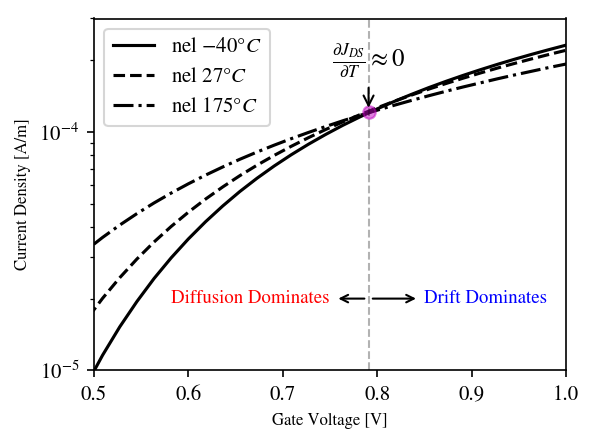
\includegraphics[width=0.6\textwidth]{jds_nel}
    %% Creator: Matplotlib, PGF backend
%%
%% To include the figure in your LaTeX document, write
%%   \input{<filename>.pgf}
%%
%% Make sure the required packages are loaded in your preamble
%%   \usepackage{pgf}
%%
%% Figures using additional raster images can only be included by \input if
%% they are in the same directory as the main LaTeX file. For loading figures
%% from other directories you can use the `import` package
%%   \usepackage{import}
%% and then include the figures with
%%   \import{<path to file>}{<filename>.pgf}
%%
%% Matplotlib used the following preamble
%%   \usepackage{gensymb}
%%   \usepackage[utf8x]{inputenc}
%%   \usepackage[T1]{fontenc}
%%
\begingroup%
\makeatletter%
\begin{pgfpicture}%
\pgfpathrectangle{\pgfpointorigin}{\pgfqpoint{3.930000in}{2.930000in}}%
\pgfusepath{use as bounding box, clip}%
\begin{pgfscope}%
\pgfsetbuttcap%
\pgfsetmiterjoin%
\definecolor{currentfill}{rgb}{1.000000,1.000000,1.000000}%
\pgfsetfillcolor{currentfill}%
\pgfsetlinewidth{0.000000pt}%
\definecolor{currentstroke}{rgb}{1.000000,1.000000,1.000000}%
\pgfsetstrokecolor{currentstroke}%
\pgfsetdash{}{0pt}%
\pgfpathmoveto{\pgfqpoint{0.000000in}{0.000000in}}%
\pgfpathlineto{\pgfqpoint{3.930000in}{0.000000in}}%
\pgfpathlineto{\pgfqpoint{3.930000in}{2.930000in}}%
\pgfpathlineto{\pgfqpoint{0.000000in}{2.930000in}}%
\pgfpathclose%
\pgfusepath{fill}%
\end{pgfscope}%
\begin{pgfscope}%
\pgfsetbuttcap%
\pgfsetmiterjoin%
\definecolor{currentfill}{rgb}{1.000000,1.000000,1.000000}%
\pgfsetfillcolor{currentfill}%
\pgfsetlinewidth{0.000000pt}%
\definecolor{currentstroke}{rgb}{0.000000,0.000000,0.000000}%
\pgfsetstrokecolor{currentstroke}%
\pgfsetstrokeopacity{0.000000}%
\pgfsetdash{}{0pt}%
\pgfpathmoveto{\pgfqpoint{0.665750in}{0.500402in}}%
\pgfpathlineto{\pgfqpoint{3.741265in}{0.500402in}}%
\pgfpathlineto{\pgfqpoint{3.741265in}{2.806667in}}%
\pgfpathlineto{\pgfqpoint{0.665750in}{2.806667in}}%
\pgfpathclose%
\pgfusepath{fill}%
\end{pgfscope}%
\begin{pgfscope}%
\pgfsetbuttcap%
\pgfsetroundjoin%
\definecolor{currentfill}{rgb}{0.000000,0.000000,0.000000}%
\pgfsetfillcolor{currentfill}%
\pgfsetlinewidth{0.803000pt}%
\definecolor{currentstroke}{rgb}{0.000000,0.000000,0.000000}%
\pgfsetstrokecolor{currentstroke}%
\pgfsetdash{}{0pt}%
\pgfsys@defobject{currentmarker}{\pgfqpoint{0.000000in}{-0.048611in}}{\pgfqpoint{0.000000in}{0.000000in}}{%
\pgfpathmoveto{\pgfqpoint{0.000000in}{0.000000in}}%
\pgfpathlineto{\pgfqpoint{0.000000in}{-0.048611in}}%
\pgfusepath{stroke,fill}%
}%
\begin{pgfscope}%
\pgfsys@transformshift{0.665750in}{0.500402in}%
\pgfsys@useobject{currentmarker}{}%
\end{pgfscope}%
\end{pgfscope}%
\begin{pgfscope}%
\pgftext[x=0.665750in,y=0.403180in,,top]{\fontsize{10.000000}{12.000000}\selectfont \(\displaystyle 0.5\)}%
\end{pgfscope}%
\begin{pgfscope}%
\pgfsetbuttcap%
\pgfsetroundjoin%
\definecolor{currentfill}{rgb}{0.000000,0.000000,0.000000}%
\pgfsetfillcolor{currentfill}%
\pgfsetlinewidth{0.803000pt}%
\definecolor{currentstroke}{rgb}{0.000000,0.000000,0.000000}%
\pgfsetstrokecolor{currentstroke}%
\pgfsetdash{}{0pt}%
\pgfsys@defobject{currentmarker}{\pgfqpoint{0.000000in}{-0.048611in}}{\pgfqpoint{0.000000in}{0.000000in}}{%
\pgfpathmoveto{\pgfqpoint{0.000000in}{0.000000in}}%
\pgfpathlineto{\pgfqpoint{0.000000in}{-0.048611in}}%
\pgfusepath{stroke,fill}%
}%
\begin{pgfscope}%
\pgfsys@transformshift{1.280853in}{0.500402in}%
\pgfsys@useobject{currentmarker}{}%
\end{pgfscope}%
\end{pgfscope}%
\begin{pgfscope}%
\pgftext[x=1.280853in,y=0.403180in,,top]{\fontsize{10.000000}{12.000000}\selectfont \(\displaystyle 0.6\)}%
\end{pgfscope}%
\begin{pgfscope}%
\pgfsetbuttcap%
\pgfsetroundjoin%
\definecolor{currentfill}{rgb}{0.000000,0.000000,0.000000}%
\pgfsetfillcolor{currentfill}%
\pgfsetlinewidth{0.803000pt}%
\definecolor{currentstroke}{rgb}{0.000000,0.000000,0.000000}%
\pgfsetstrokecolor{currentstroke}%
\pgfsetdash{}{0pt}%
\pgfsys@defobject{currentmarker}{\pgfqpoint{0.000000in}{-0.048611in}}{\pgfqpoint{0.000000in}{0.000000in}}{%
\pgfpathmoveto{\pgfqpoint{0.000000in}{0.000000in}}%
\pgfpathlineto{\pgfqpoint{0.000000in}{-0.048611in}}%
\pgfusepath{stroke,fill}%
}%
\begin{pgfscope}%
\pgfsys@transformshift{1.895956in}{0.500402in}%
\pgfsys@useobject{currentmarker}{}%
\end{pgfscope}%
\end{pgfscope}%
\begin{pgfscope}%
\pgftext[x=1.895956in,y=0.403180in,,top]{\fontsize{10.000000}{12.000000}\selectfont \(\displaystyle 0.7\)}%
\end{pgfscope}%
\begin{pgfscope}%
\pgfsetbuttcap%
\pgfsetroundjoin%
\definecolor{currentfill}{rgb}{0.000000,0.000000,0.000000}%
\pgfsetfillcolor{currentfill}%
\pgfsetlinewidth{0.803000pt}%
\definecolor{currentstroke}{rgb}{0.000000,0.000000,0.000000}%
\pgfsetstrokecolor{currentstroke}%
\pgfsetdash{}{0pt}%
\pgfsys@defobject{currentmarker}{\pgfqpoint{0.000000in}{-0.048611in}}{\pgfqpoint{0.000000in}{0.000000in}}{%
\pgfpathmoveto{\pgfqpoint{0.000000in}{0.000000in}}%
\pgfpathlineto{\pgfqpoint{0.000000in}{-0.048611in}}%
\pgfusepath{stroke,fill}%
}%
\begin{pgfscope}%
\pgfsys@transformshift{2.511059in}{0.500402in}%
\pgfsys@useobject{currentmarker}{}%
\end{pgfscope}%
\end{pgfscope}%
\begin{pgfscope}%
\pgftext[x=2.511059in,y=0.403180in,,top]{\fontsize{10.000000}{12.000000}\selectfont \(\displaystyle 0.8\)}%
\end{pgfscope}%
\begin{pgfscope}%
\pgfsetbuttcap%
\pgfsetroundjoin%
\definecolor{currentfill}{rgb}{0.000000,0.000000,0.000000}%
\pgfsetfillcolor{currentfill}%
\pgfsetlinewidth{0.803000pt}%
\definecolor{currentstroke}{rgb}{0.000000,0.000000,0.000000}%
\pgfsetstrokecolor{currentstroke}%
\pgfsetdash{}{0pt}%
\pgfsys@defobject{currentmarker}{\pgfqpoint{0.000000in}{-0.048611in}}{\pgfqpoint{0.000000in}{0.000000in}}{%
\pgfpathmoveto{\pgfqpoint{0.000000in}{0.000000in}}%
\pgfpathlineto{\pgfqpoint{0.000000in}{-0.048611in}}%
\pgfusepath{stroke,fill}%
}%
\begin{pgfscope}%
\pgfsys@transformshift{3.126162in}{0.500402in}%
\pgfsys@useobject{currentmarker}{}%
\end{pgfscope}%
\end{pgfscope}%
\begin{pgfscope}%
\pgftext[x=3.126162in,y=0.403180in,,top]{\fontsize{10.000000}{12.000000}\selectfont \(\displaystyle 0.9\)}%
\end{pgfscope}%
\begin{pgfscope}%
\pgfsetbuttcap%
\pgfsetroundjoin%
\definecolor{currentfill}{rgb}{0.000000,0.000000,0.000000}%
\pgfsetfillcolor{currentfill}%
\pgfsetlinewidth{0.803000pt}%
\definecolor{currentstroke}{rgb}{0.000000,0.000000,0.000000}%
\pgfsetstrokecolor{currentstroke}%
\pgfsetdash{}{0pt}%
\pgfsys@defobject{currentmarker}{\pgfqpoint{0.000000in}{-0.048611in}}{\pgfqpoint{0.000000in}{0.000000in}}{%
\pgfpathmoveto{\pgfqpoint{0.000000in}{0.000000in}}%
\pgfpathlineto{\pgfqpoint{0.000000in}{-0.048611in}}%
\pgfusepath{stroke,fill}%
}%
\begin{pgfscope}%
\pgfsys@transformshift{3.741265in}{0.500402in}%
\pgfsys@useobject{currentmarker}{}%
\end{pgfscope}%
\end{pgfscope}%
\begin{pgfscope}%
\pgftext[x=3.741265in,y=0.403180in,,top]{\fontsize{10.000000}{12.000000}\selectfont \(\displaystyle 1.0\)}%
\end{pgfscope}%
\begin{pgfscope}%
\pgftext[x=2.203507in,y=0.224969in,,top]{\fontsize{9.000000}{10.800000}\selectfont Gate Voltage [V]}%
\end{pgfscope}%
\begin{pgfscope}%
\pgfsetbuttcap%
\pgfsetroundjoin%
\definecolor{currentfill}{rgb}{0.000000,0.000000,0.000000}%
\pgfsetfillcolor{currentfill}%
\pgfsetlinewidth{0.803000pt}%
\definecolor{currentstroke}{rgb}{0.000000,0.000000,0.000000}%
\pgfsetstrokecolor{currentstroke}%
\pgfsetdash{}{0pt}%
\pgfsys@defobject{currentmarker}{\pgfqpoint{-0.048611in}{0.000000in}}{\pgfqpoint{0.000000in}{0.000000in}}{%
\pgfpathmoveto{\pgfqpoint{0.000000in}{0.000000in}}%
\pgfpathlineto{\pgfqpoint{-0.048611in}{0.000000in}}%
\pgfusepath{stroke,fill}%
}%
\begin{pgfscope}%
\pgfsys@transformshift{0.665750in}{0.500402in}%
\pgfsys@useobject{currentmarker}{}%
\end{pgfscope}%
\end{pgfscope}%
\begin{pgfscope}%
\pgftext[x=0.280525in,y=0.452575in,left,base]{\fontsize{10.000000}{12.000000}\selectfont \(\displaystyle 10^{-5}\)}%
\end{pgfscope}%
\begin{pgfscope}%
\pgfsetbuttcap%
\pgfsetroundjoin%
\definecolor{currentfill}{rgb}{0.000000,0.000000,0.000000}%
\pgfsetfillcolor{currentfill}%
\pgfsetlinewidth{0.803000pt}%
\definecolor{currentstroke}{rgb}{0.000000,0.000000,0.000000}%
\pgfsetstrokecolor{currentstroke}%
\pgfsetdash{}{0pt}%
\pgfsys@defobject{currentmarker}{\pgfqpoint{-0.048611in}{0.000000in}}{\pgfqpoint{0.000000in}{0.000000in}}{%
\pgfpathmoveto{\pgfqpoint{0.000000in}{0.000000in}}%
\pgfpathlineto{\pgfqpoint{-0.048611in}{0.000000in}}%
\pgfusepath{stroke,fill}%
}%
\begin{pgfscope}%
\pgfsys@transformshift{0.665750in}{2.061726in}%
\pgfsys@useobject{currentmarker}{}%
\end{pgfscope}%
\end{pgfscope}%
\begin{pgfscope}%
\pgftext[x=0.280525in,y=2.013898in,left,base]{\fontsize{10.000000}{12.000000}\selectfont \(\displaystyle 10^{-4}\)}%
\end{pgfscope}%
\begin{pgfscope}%
\pgfsetbuttcap%
\pgfsetroundjoin%
\definecolor{currentfill}{rgb}{0.000000,0.000000,0.000000}%
\pgfsetfillcolor{currentfill}%
\pgfsetlinewidth{0.602250pt}%
\definecolor{currentstroke}{rgb}{0.000000,0.000000,0.000000}%
\pgfsetstrokecolor{currentstroke}%
\pgfsetdash{}{0pt}%
\pgfsys@defobject{currentmarker}{\pgfqpoint{-0.027778in}{0.000000in}}{\pgfqpoint{0.000000in}{0.000000in}}{%
\pgfpathmoveto{\pgfqpoint{0.000000in}{0.000000in}}%
\pgfpathlineto{\pgfqpoint{-0.027778in}{0.000000in}}%
\pgfusepath{stroke,fill}%
}%
\begin{pgfscope}%
\pgfsys@transformshift{0.665750in}{0.970408in}%
\pgfsys@useobject{currentmarker}{}%
\end{pgfscope}%
\end{pgfscope}%
\begin{pgfscope}%
\pgfsetbuttcap%
\pgfsetroundjoin%
\definecolor{currentfill}{rgb}{0.000000,0.000000,0.000000}%
\pgfsetfillcolor{currentfill}%
\pgfsetlinewidth{0.602250pt}%
\definecolor{currentstroke}{rgb}{0.000000,0.000000,0.000000}%
\pgfsetstrokecolor{currentstroke}%
\pgfsetdash{}{0pt}%
\pgfsys@defobject{currentmarker}{\pgfqpoint{-0.027778in}{0.000000in}}{\pgfqpoint{0.000000in}{0.000000in}}{%
\pgfpathmoveto{\pgfqpoint{0.000000in}{0.000000in}}%
\pgfpathlineto{\pgfqpoint{-0.027778in}{0.000000in}}%
\pgfusepath{stroke,fill}%
}%
\begin{pgfscope}%
\pgfsys@transformshift{0.665750in}{1.245343in}%
\pgfsys@useobject{currentmarker}{}%
\end{pgfscope}%
\end{pgfscope}%
\begin{pgfscope}%
\pgfsetbuttcap%
\pgfsetroundjoin%
\definecolor{currentfill}{rgb}{0.000000,0.000000,0.000000}%
\pgfsetfillcolor{currentfill}%
\pgfsetlinewidth{0.602250pt}%
\definecolor{currentstroke}{rgb}{0.000000,0.000000,0.000000}%
\pgfsetstrokecolor{currentstroke}%
\pgfsetdash{}{0pt}%
\pgfsys@defobject{currentmarker}{\pgfqpoint{-0.027778in}{0.000000in}}{\pgfqpoint{0.000000in}{0.000000in}}{%
\pgfpathmoveto{\pgfqpoint{0.000000in}{0.000000in}}%
\pgfpathlineto{\pgfqpoint{-0.027778in}{0.000000in}}%
\pgfusepath{stroke,fill}%
}%
\begin{pgfscope}%
\pgfsys@transformshift{0.665750in}{1.440413in}%
\pgfsys@useobject{currentmarker}{}%
\end{pgfscope}%
\end{pgfscope}%
\begin{pgfscope}%
\pgfsetbuttcap%
\pgfsetroundjoin%
\definecolor{currentfill}{rgb}{0.000000,0.000000,0.000000}%
\pgfsetfillcolor{currentfill}%
\pgfsetlinewidth{0.602250pt}%
\definecolor{currentstroke}{rgb}{0.000000,0.000000,0.000000}%
\pgfsetstrokecolor{currentstroke}%
\pgfsetdash{}{0pt}%
\pgfsys@defobject{currentmarker}{\pgfqpoint{-0.027778in}{0.000000in}}{\pgfqpoint{0.000000in}{0.000000in}}{%
\pgfpathmoveto{\pgfqpoint{0.000000in}{0.000000in}}%
\pgfpathlineto{\pgfqpoint{-0.027778in}{0.000000in}}%
\pgfusepath{stroke,fill}%
}%
\begin{pgfscope}%
\pgfsys@transformshift{0.665750in}{1.591721in}%
\pgfsys@useobject{currentmarker}{}%
\end{pgfscope}%
\end{pgfscope}%
\begin{pgfscope}%
\pgfsetbuttcap%
\pgfsetroundjoin%
\definecolor{currentfill}{rgb}{0.000000,0.000000,0.000000}%
\pgfsetfillcolor{currentfill}%
\pgfsetlinewidth{0.602250pt}%
\definecolor{currentstroke}{rgb}{0.000000,0.000000,0.000000}%
\pgfsetstrokecolor{currentstroke}%
\pgfsetdash{}{0pt}%
\pgfsys@defobject{currentmarker}{\pgfqpoint{-0.027778in}{0.000000in}}{\pgfqpoint{0.000000in}{0.000000in}}{%
\pgfpathmoveto{\pgfqpoint{0.000000in}{0.000000in}}%
\pgfpathlineto{\pgfqpoint{-0.027778in}{0.000000in}}%
\pgfusepath{stroke,fill}%
}%
\begin{pgfscope}%
\pgfsys@transformshift{0.665750in}{1.715348in}%
\pgfsys@useobject{currentmarker}{}%
\end{pgfscope}%
\end{pgfscope}%
\begin{pgfscope}%
\pgfsetbuttcap%
\pgfsetroundjoin%
\definecolor{currentfill}{rgb}{0.000000,0.000000,0.000000}%
\pgfsetfillcolor{currentfill}%
\pgfsetlinewidth{0.602250pt}%
\definecolor{currentstroke}{rgb}{0.000000,0.000000,0.000000}%
\pgfsetstrokecolor{currentstroke}%
\pgfsetdash{}{0pt}%
\pgfsys@defobject{currentmarker}{\pgfqpoint{-0.027778in}{0.000000in}}{\pgfqpoint{0.000000in}{0.000000in}}{%
\pgfpathmoveto{\pgfqpoint{0.000000in}{0.000000in}}%
\pgfpathlineto{\pgfqpoint{-0.027778in}{0.000000in}}%
\pgfusepath{stroke,fill}%
}%
\begin{pgfscope}%
\pgfsys@transformshift{0.665750in}{1.819874in}%
\pgfsys@useobject{currentmarker}{}%
\end{pgfscope}%
\end{pgfscope}%
\begin{pgfscope}%
\pgfsetbuttcap%
\pgfsetroundjoin%
\definecolor{currentfill}{rgb}{0.000000,0.000000,0.000000}%
\pgfsetfillcolor{currentfill}%
\pgfsetlinewidth{0.602250pt}%
\definecolor{currentstroke}{rgb}{0.000000,0.000000,0.000000}%
\pgfsetstrokecolor{currentstroke}%
\pgfsetdash{}{0pt}%
\pgfsys@defobject{currentmarker}{\pgfqpoint{-0.027778in}{0.000000in}}{\pgfqpoint{0.000000in}{0.000000in}}{%
\pgfpathmoveto{\pgfqpoint{0.000000in}{0.000000in}}%
\pgfpathlineto{\pgfqpoint{-0.027778in}{0.000000in}}%
\pgfusepath{stroke,fill}%
}%
\begin{pgfscope}%
\pgfsys@transformshift{0.665750in}{1.910418in}%
\pgfsys@useobject{currentmarker}{}%
\end{pgfscope}%
\end{pgfscope}%
\begin{pgfscope}%
\pgfsetbuttcap%
\pgfsetroundjoin%
\definecolor{currentfill}{rgb}{0.000000,0.000000,0.000000}%
\pgfsetfillcolor{currentfill}%
\pgfsetlinewidth{0.602250pt}%
\definecolor{currentstroke}{rgb}{0.000000,0.000000,0.000000}%
\pgfsetstrokecolor{currentstroke}%
\pgfsetdash{}{0pt}%
\pgfsys@defobject{currentmarker}{\pgfqpoint{-0.027778in}{0.000000in}}{\pgfqpoint{0.000000in}{0.000000in}}{%
\pgfpathmoveto{\pgfqpoint{0.000000in}{0.000000in}}%
\pgfpathlineto{\pgfqpoint{-0.027778in}{0.000000in}}%
\pgfusepath{stroke,fill}%
}%
\begin{pgfscope}%
\pgfsys@transformshift{0.665750in}{1.990284in}%
\pgfsys@useobject{currentmarker}{}%
\end{pgfscope}%
\end{pgfscope}%
\begin{pgfscope}%
\pgfsetbuttcap%
\pgfsetroundjoin%
\definecolor{currentfill}{rgb}{0.000000,0.000000,0.000000}%
\pgfsetfillcolor{currentfill}%
\pgfsetlinewidth{0.602250pt}%
\definecolor{currentstroke}{rgb}{0.000000,0.000000,0.000000}%
\pgfsetstrokecolor{currentstroke}%
\pgfsetdash{}{0pt}%
\pgfsys@defobject{currentmarker}{\pgfqpoint{-0.027778in}{0.000000in}}{\pgfqpoint{0.000000in}{0.000000in}}{%
\pgfpathmoveto{\pgfqpoint{0.000000in}{0.000000in}}%
\pgfpathlineto{\pgfqpoint{-0.027778in}{0.000000in}}%
\pgfusepath{stroke,fill}%
}%
\begin{pgfscope}%
\pgfsys@transformshift{0.665750in}{2.531731in}%
\pgfsys@useobject{currentmarker}{}%
\end{pgfscope}%
\end{pgfscope}%
\begin{pgfscope}%
\pgfsetbuttcap%
\pgfsetroundjoin%
\definecolor{currentfill}{rgb}{0.000000,0.000000,0.000000}%
\pgfsetfillcolor{currentfill}%
\pgfsetlinewidth{0.602250pt}%
\definecolor{currentstroke}{rgb}{0.000000,0.000000,0.000000}%
\pgfsetstrokecolor{currentstroke}%
\pgfsetdash{}{0pt}%
\pgfsys@defobject{currentmarker}{\pgfqpoint{-0.027778in}{0.000000in}}{\pgfqpoint{0.000000in}{0.000000in}}{%
\pgfpathmoveto{\pgfqpoint{0.000000in}{0.000000in}}%
\pgfpathlineto{\pgfqpoint{-0.027778in}{0.000000in}}%
\pgfusepath{stroke,fill}%
}%
\begin{pgfscope}%
\pgfsys@transformshift{0.665750in}{2.806667in}%
\pgfsys@useobject{currentmarker}{}%
\end{pgfscope}%
\end{pgfscope}%
\begin{pgfscope}%
\pgftext[x=0.224969in,y=1.653535in,,bottom,rotate=90.000000]{\fontsize{9.000000}{10.800000}\selectfont Current Density [A/m]}%
\end{pgfscope}%
\begin{pgfscope}%
\pgfpathrectangle{\pgfqpoint{0.665750in}{0.500402in}}{\pgfqpoint{3.075515in}{2.306264in}} %
\pgfusepath{clip}%
\pgfsetrectcap%
\pgfsetroundjoin%
\pgfsetlinewidth{1.505625pt}%
\definecolor{currentstroke}{rgb}{0.000000,0.000000,0.000000}%
\pgfsetstrokecolor{currentstroke}%
\pgfsetdash{}{0pt}%
\pgfpathmoveto{\pgfqpoint{0.664776in}{0.493736in}}%
\pgfpathlineto{\pgfqpoint{0.721724in}{0.599286in}}%
\pgfpathlineto{\pgfqpoint{0.833673in}{0.785211in}}%
\pgfpathlineto{\pgfqpoint{0.945622in}{0.951499in}}%
\pgfpathlineto{\pgfqpoint{1.056955in}{1.101900in}}%
\pgfpathlineto{\pgfqpoint{1.168904in}{1.237843in}}%
\pgfpathlineto{\pgfqpoint{1.280853in}{1.361585in}}%
\pgfpathlineto{\pgfqpoint{1.392802in}{1.474303in}}%
\pgfpathlineto{\pgfqpoint{1.504750in}{1.577607in}}%
\pgfpathlineto{\pgfqpoint{1.616084in}{1.672309in}}%
\pgfpathlineto{\pgfqpoint{1.728033in}{1.759322in}}%
\pgfpathlineto{\pgfqpoint{1.839982in}{1.839635in}}%
\pgfpathlineto{\pgfqpoint{1.951930in}{1.913884in}}%
\pgfpathlineto{\pgfqpoint{2.063879in}{1.982707in}}%
\pgfpathlineto{\pgfqpoint{2.175828in}{2.046711in}}%
\pgfpathlineto{\pgfqpoint{2.287161in}{2.106335in}}%
\pgfpathlineto{\pgfqpoint{2.399110in}{2.161781in}}%
\pgfpathlineto{\pgfqpoint{2.511059in}{2.214118in}}%
\pgfpathlineto{\pgfqpoint{2.623008in}{2.263207in}}%
\pgfpathlineto{\pgfqpoint{2.734956in}{2.309452in}}%
\pgfpathlineto{\pgfqpoint{2.846290in}{2.353184in}}%
\pgfpathlineto{\pgfqpoint{2.958239in}{2.394266in}}%
\pgfpathlineto{\pgfqpoint{3.070188in}{2.433393in}}%
\pgfpathlineto{\pgfqpoint{3.182136in}{2.470385in}}%
\pgfpathlineto{\pgfqpoint{3.294085in}{2.505814in}}%
\pgfpathlineto{\pgfqpoint{3.406034in}{2.539485in}}%
\pgfpathlineto{\pgfqpoint{3.517368in}{2.571562in}}%
\pgfpathlineto{\pgfqpoint{3.629316in}{2.602190in}}%
\pgfpathlineto{\pgfqpoint{3.747932in}{2.633494in}}%
\pgfpathlineto{\pgfqpoint{3.747932in}{2.633494in}}%
\pgfusepath{stroke}%
\end{pgfscope}%
\begin{pgfscope}%
\pgfpathrectangle{\pgfqpoint{0.665750in}{0.500402in}}{\pgfqpoint{3.075515in}{2.306264in}} %
\pgfusepath{clip}%
\pgfsetbuttcap%
\pgfsetroundjoin%
\pgfsetlinewidth{1.505625pt}%
\definecolor{currentstroke}{rgb}{0.000000,0.000000,0.000000}%
\pgfsetstrokecolor{currentstroke}%
\pgfsetdash{{5.550000pt}{2.400000pt}}{0.000000pt}%
\pgfpathmoveto{\pgfqpoint{0.659083in}{0.888766in}}%
\pgfpathlineto{\pgfqpoint{0.721724in}{0.972439in}}%
\pgfpathlineto{\pgfqpoint{0.833673in}{1.107463in}}%
\pgfpathlineto{\pgfqpoint{0.945622in}{1.230028in}}%
\pgfpathlineto{\pgfqpoint{1.056955in}{1.341486in}}%
\pgfpathlineto{\pgfqpoint{1.168904in}{1.443457in}}%
\pgfpathlineto{\pgfqpoint{1.280853in}{1.536801in}}%
\pgfpathlineto{\pgfqpoint{1.392802in}{1.622864in}}%
\pgfpathlineto{\pgfqpoint{1.504750in}{1.702456in}}%
\pgfpathlineto{\pgfqpoint{1.616084in}{1.776267in}}%
\pgfpathlineto{\pgfqpoint{1.728033in}{1.844977in}}%
\pgfpathlineto{\pgfqpoint{1.839982in}{1.909146in}}%
\pgfpathlineto{\pgfqpoint{1.951930in}{1.969242in}}%
\pgfpathlineto{\pgfqpoint{2.063879in}{2.025731in}}%
\pgfpathlineto{\pgfqpoint{2.175828in}{2.079131in}}%
\pgfpathlineto{\pgfqpoint{2.287161in}{2.128815in}}%
\pgfpathlineto{\pgfqpoint{2.399110in}{2.176252in}}%
\pgfpathlineto{\pgfqpoint{2.511059in}{2.221122in}}%
\pgfpathlineto{\pgfqpoint{2.623008in}{2.264214in}}%
\pgfpathlineto{\pgfqpoint{2.734956in}{2.304730in}}%
\pgfpathlineto{\pgfqpoint{2.846290in}{2.343408in}}%
\pgfpathlineto{\pgfqpoint{2.958239in}{2.379999in}}%
\pgfpathlineto{\pgfqpoint{3.070188in}{2.415119in}}%
\pgfpathlineto{\pgfqpoint{3.182136in}{2.448892in}}%
\pgfpathlineto{\pgfqpoint{3.294085in}{2.481428in}}%
\pgfpathlineto{\pgfqpoint{3.406034in}{2.512125in}}%
\pgfpathlineto{\pgfqpoint{3.517368in}{2.541827in}}%
\pgfpathlineto{\pgfqpoint{3.629316in}{2.570602in}}%
\pgfpathlineto{\pgfqpoint{3.747932in}{2.599785in}}%
\pgfpathlineto{\pgfqpoint{3.747932in}{2.599785in}}%
\pgfusepath{stroke}%
\end{pgfscope}%
\begin{pgfscope}%
\pgfpathrectangle{\pgfqpoint{0.665750in}{0.500402in}}{\pgfqpoint{3.075515in}{2.306264in}} %
\pgfusepath{clip}%
\pgfsetbuttcap%
\pgfsetroundjoin%
\pgfsetlinewidth{1.505625pt}%
\definecolor{currentstroke}{rgb}{0.000000,0.000000,0.000000}%
\pgfsetstrokecolor{currentstroke}%
\pgfsetdash{{9.600000pt}{2.400000pt}{1.500000pt}{2.400000pt}}{0.000000pt}%
\pgfpathmoveto{\pgfqpoint{0.659083in}{1.322382in}}%
\pgfpathlineto{\pgfqpoint{0.721724in}{1.371415in}}%
\pgfpathlineto{\pgfqpoint{0.833673in}{1.452510in}}%
\pgfpathlineto{\pgfqpoint{0.945622in}{1.527622in}}%
\pgfpathlineto{\pgfqpoint{1.056955in}{1.597393in}}%
\pgfpathlineto{\pgfqpoint{1.168904in}{1.662362in}}%
\pgfpathlineto{\pgfqpoint{1.280853in}{1.723102in}}%
\pgfpathlineto{\pgfqpoint{1.392802in}{1.779976in}}%
\pgfpathlineto{\pgfqpoint{1.504750in}{1.833397in}}%
\pgfpathlineto{\pgfqpoint{1.616084in}{1.883708in}}%
\pgfpathlineto{\pgfqpoint{1.728033in}{1.931284in}}%
\pgfpathlineto{\pgfqpoint{1.839982in}{1.976354in}}%
\pgfpathlineto{\pgfqpoint{1.951930in}{2.019120in}}%
\pgfpathlineto{\pgfqpoint{2.063879in}{2.059825in}}%
\pgfpathlineto{\pgfqpoint{2.175828in}{2.098673in}}%
\pgfpathlineto{\pgfqpoint{2.287161in}{2.136145in}}%
\pgfpathlineto{\pgfqpoint{2.399110in}{2.171655in}}%
\pgfpathlineto{\pgfqpoint{2.511059in}{2.205397in}}%
\pgfpathlineto{\pgfqpoint{2.623008in}{2.238062in}}%
\pgfpathlineto{\pgfqpoint{2.734956in}{2.269725in}}%
\pgfpathlineto{\pgfqpoint{2.846290in}{2.299975in}}%
\pgfpathlineto{\pgfqpoint{2.958239in}{2.329390in}}%
\pgfpathlineto{\pgfqpoint{3.070188in}{2.357582in}}%
\pgfpathlineto{\pgfqpoint{3.294085in}{2.411081in}}%
\pgfpathlineto{\pgfqpoint{3.406034in}{2.436521in}}%
\pgfpathlineto{\pgfqpoint{3.629316in}{2.485070in}}%
\pgfpathlineto{\pgfqpoint{3.747932in}{2.509627in}}%
\pgfpathlineto{\pgfqpoint{3.747932in}{2.509627in}}%
\pgfusepath{stroke}%
\end{pgfscope}%
\begin{pgfscope}%
\pgfpathrectangle{\pgfqpoint{0.665750in}{0.500402in}}{\pgfqpoint{3.075515in}{2.306264in}} %
\pgfusepath{clip}%
\pgfsetbuttcap%
\pgfsetroundjoin%
\definecolor{currentfill}{rgb}{0.750000,0.000000,0.750000}%
\pgfsetfillcolor{currentfill}%
\pgfsetfillopacity{0.500000}%
\pgfsetlinewidth{1.003750pt}%
\definecolor{currentstroke}{rgb}{0.750000,0.000000,0.750000}%
\pgfsetstrokecolor{currentstroke}%
\pgfsetstrokeopacity{0.500000}%
\pgfsetdash{}{0pt}%
\pgfsys@defobject{currentmarker}{\pgfqpoint{-0.041667in}{-0.041667in}}{\pgfqpoint{0.041667in}{0.041667in}}{%
\pgfpathmoveto{\pgfqpoint{0.000000in}{-0.041667in}}%
\pgfpathcurveto{\pgfqpoint{0.011050in}{-0.041667in}}{\pgfqpoint{0.021649in}{-0.037276in}}{\pgfqpoint{0.029463in}{-0.029463in}}%
\pgfpathcurveto{\pgfqpoint{0.037276in}{-0.021649in}}{\pgfqpoint{0.041667in}{-0.011050in}}{\pgfqpoint{0.041667in}{0.000000in}}%
\pgfpathcurveto{\pgfqpoint{0.041667in}{0.011050in}}{\pgfqpoint{0.037276in}{0.021649in}}{\pgfqpoint{0.029463in}{0.029463in}}%
\pgfpathcurveto{\pgfqpoint{0.021649in}{0.037276in}}{\pgfqpoint{0.011050in}{0.041667in}}{\pgfqpoint{0.000000in}{0.041667in}}%
\pgfpathcurveto{\pgfqpoint{-0.011050in}{0.041667in}}{\pgfqpoint{-0.021649in}{0.037276in}}{\pgfqpoint{-0.029463in}{0.029463in}}%
\pgfpathcurveto{\pgfqpoint{-0.037276in}{0.021649in}}{\pgfqpoint{-0.041667in}{0.011050in}}{\pgfqpoint{-0.041667in}{0.000000in}}%
\pgfpathcurveto{\pgfqpoint{-0.041667in}{-0.011050in}}{\pgfqpoint{-0.037276in}{-0.021649in}}{\pgfqpoint{-0.029463in}{-0.029463in}}%
\pgfpathcurveto{\pgfqpoint{-0.021649in}{-0.037276in}}{\pgfqpoint{-0.011050in}{-0.041667in}}{\pgfqpoint{0.000000in}{-0.041667in}}%
\pgfpathclose%
\pgfusepath{stroke,fill}%
}%
\begin{pgfscope}%
\pgfsys@transformshift{2.455085in}{2.193654in}%
\pgfsys@useobject{currentmarker}{}%
\end{pgfscope}%
\end{pgfscope}%
\begin{pgfscope}%
\pgfpathrectangle{\pgfqpoint{0.665750in}{0.500402in}}{\pgfqpoint{3.075515in}{2.306264in}} %
\pgfusepath{clip}%
\pgfsetbuttcap%
\pgfsetroundjoin%
\pgfsetlinewidth{1.003750pt}%
\definecolor{currentstroke}{rgb}{0.000000,0.000000,0.000000}%
\pgfsetstrokecolor{currentstroke}%
\pgfsetstrokeopacity{0.300000}%
\pgfsetdash{{3.700000pt}{1.600000pt}}{0.000000pt}%
\pgfpathmoveto{\pgfqpoint{2.455085in}{0.500402in}}%
\pgfpathlineto{\pgfqpoint{2.455085in}{2.806667in}}%
\pgfusepath{stroke}%
\end{pgfscope}%
\begin{pgfscope}%
\pgfsetrectcap%
\pgfsetmiterjoin%
\pgfsetlinewidth{0.803000pt}%
\definecolor{currentstroke}{rgb}{0.000000,0.000000,0.000000}%
\pgfsetstrokecolor{currentstroke}%
\pgfsetdash{}{0pt}%
\pgfpathmoveto{\pgfqpoint{0.665750in}{0.500402in}}%
\pgfpathlineto{\pgfqpoint{0.665750in}{2.806667in}}%
\pgfusepath{stroke}%
\end{pgfscope}%
\begin{pgfscope}%
\pgfsetrectcap%
\pgfsetmiterjoin%
\pgfsetlinewidth{0.803000pt}%
\definecolor{currentstroke}{rgb}{0.000000,0.000000,0.000000}%
\pgfsetstrokecolor{currentstroke}%
\pgfsetdash{}{0pt}%
\pgfpathmoveto{\pgfqpoint{3.741265in}{0.500402in}}%
\pgfpathlineto{\pgfqpoint{3.741265in}{2.806667in}}%
\pgfusepath{stroke}%
\end{pgfscope}%
\begin{pgfscope}%
\pgfsetrectcap%
\pgfsetmiterjoin%
\pgfsetlinewidth{0.803000pt}%
\definecolor{currentstroke}{rgb}{0.000000,0.000000,0.000000}%
\pgfsetstrokecolor{currentstroke}%
\pgfsetdash{}{0pt}%
\pgfpathmoveto{\pgfqpoint{0.665750in}{0.500402in}}%
\pgfpathlineto{\pgfqpoint{3.741265in}{0.500402in}}%
\pgfusepath{stroke}%
\end{pgfscope}%
\begin{pgfscope}%
\pgfsetrectcap%
\pgfsetmiterjoin%
\pgfsetlinewidth{0.803000pt}%
\definecolor{currentstroke}{rgb}{0.000000,0.000000,0.000000}%
\pgfsetstrokecolor{currentstroke}%
\pgfsetdash{}{0pt}%
\pgfpathmoveto{\pgfqpoint{0.665750in}{2.806667in}}%
\pgfpathlineto{\pgfqpoint{3.741265in}{2.806667in}}%
\pgfusepath{stroke}%
\end{pgfscope}%
\begin{pgfscope}%
\pgfsetroundcap%
\pgfsetroundjoin%
\pgfsetlinewidth{1.003750pt}%
\definecolor{currentstroke}{rgb}{0.000000,0.000000,0.000000}%
\pgfsetstrokecolor{currentstroke}%
\pgfsetdash{}{0pt}%
\pgfpathmoveto{\pgfqpoint{2.455085in}{2.349939in}}%
\pgfpathquadraticcurveto{\pgfqpoint{2.455085in}{2.285695in}}{\pgfqpoint{2.455085in}{2.236979in}}%
\pgfusepath{stroke}%
\end{pgfscope}%
\begin{pgfscope}%
\pgfsetroundcap%
\pgfsetroundjoin%
\pgfsetlinewidth{1.003750pt}%
\definecolor{currentstroke}{rgb}{0.000000,0.000000,0.000000}%
\pgfsetstrokecolor{currentstroke}%
\pgfsetdash{}{0pt}%
\pgfpathmoveto{\pgfqpoint{2.480085in}{2.286979in}}%
\pgfpathlineto{\pgfqpoint{2.455085in}{2.236979in}}%
\pgfpathlineto{\pgfqpoint{2.430085in}{2.286979in}}%
\pgfusepath{stroke}%
\end{pgfscope}%
\begin{pgfscope}%
\pgftext[x=2.455085in,y=2.531731in,,]{\fontsize{9.000000}{10.800000}\selectfont \(\displaystyle \frac{\partial J_{DS}}{\partial T} \approx 0 \)}%
\end{pgfscope}%
\begin{pgfscope}%
\pgfsetroundcap%
\pgfsetroundjoin%
\pgfsetlinewidth{1.003750pt}%
\definecolor{currentstroke}{rgb}{0.000000,0.000000,0.000000}%
\pgfsetstrokecolor{currentstroke}%
\pgfsetdash{}{0pt}%
\pgfpathmoveto{\pgfqpoint{2.747536in}{0.970408in}}%
\pgfpathquadraticcurveto{\pgfqpoint{2.622956in}{0.970408in}}{\pgfqpoint{2.482849in}{0.970408in}}%
\pgfusepath{stroke}%
\end{pgfscope}%
\begin{pgfscope}%
\pgfsetroundcap%
\pgfsetroundjoin%
\pgfsetlinewidth{1.003750pt}%
\definecolor{currentstroke}{rgb}{0.000000,0.000000,0.000000}%
\pgfsetstrokecolor{currentstroke}%
\pgfsetdash{}{0pt}%
\pgfpathmoveto{\pgfqpoint{2.697536in}{0.995408in}}%
\pgfpathlineto{\pgfqpoint{2.747536in}{0.970408in}}%
\pgfpathlineto{\pgfqpoint{2.697536in}{0.945408in}}%
\pgfusepath{stroke}%
\end{pgfscope}%
\begin{pgfscope}%
\definecolor{textcolor}{rgb}{0.000000,0.000000,1.000000}%
\pgfsetstrokecolor{textcolor}%
\pgfsetfillcolor{textcolor}%
\pgftext[x=2.818611in,y=0.970408in,left,]{\color{textcolor}\fontsize{9.000000}{10.800000}\selectfont Drift Dominates}%
\end{pgfscope}%
\begin{pgfscope}%
\pgfsetroundcap%
\pgfsetroundjoin%
\pgfsetlinewidth{1.003750pt}%
\definecolor{currentstroke}{rgb}{0.000000,0.000000,0.000000}%
\pgfsetstrokecolor{currentstroke}%
\pgfsetdash{}{0pt}%
\pgfpathmoveto{\pgfqpoint{2.274597in}{0.970408in}}%
\pgfpathquadraticcurveto{\pgfqpoint{2.343187in}{0.970408in}}{\pgfqpoint{2.427304in}{0.970408in}}%
\pgfusepath{stroke}%
\end{pgfscope}%
\begin{pgfscope}%
\pgfsetroundcap%
\pgfsetroundjoin%
\pgfsetlinewidth{1.003750pt}%
\definecolor{currentstroke}{rgb}{0.000000,0.000000,0.000000}%
\pgfsetstrokecolor{currentstroke}%
\pgfsetdash{}{0pt}%
\pgfpathmoveto{\pgfqpoint{2.324597in}{0.945408in}}%
\pgfpathlineto{\pgfqpoint{2.274597in}{0.970408in}}%
\pgfpathlineto{\pgfqpoint{2.324597in}{0.995408in}}%
\pgfusepath{stroke}%
\end{pgfscope}%
\begin{pgfscope}%
\definecolor{textcolor}{rgb}{1.000000,0.000000,0.000000}%
\pgfsetstrokecolor{textcolor}%
\pgfsetfillcolor{textcolor}%
\pgftext[x=2.203507in,y=0.970408in,right,]{\color{textcolor}\fontsize{9.000000}{10.800000}\selectfont Diffusion Dominates}%
\end{pgfscope}%
\begin{pgfscope}%
\pgfsetbuttcap%
\pgfsetmiterjoin%
\definecolor{currentfill}{rgb}{1.000000,1.000000,1.000000}%
\pgfsetfillcolor{currentfill}%
\pgfsetfillopacity{0.800000}%
\pgfsetlinewidth{1.003750pt}%
\definecolor{currentstroke}{rgb}{0.800000,0.800000,0.800000}%
\pgfsetstrokecolor{currentstroke}%
\pgfsetstrokeopacity{0.800000}%
\pgfsetdash{}{0pt}%
\pgfpathmoveto{\pgfqpoint{0.762972in}{2.114557in}}%
\pgfpathlineto{\pgfqpoint{1.851093in}{2.114557in}}%
\pgfpathquadraticcurveto{\pgfqpoint{1.878871in}{2.114557in}}{\pgfqpoint{1.878871in}{2.142335in}}%
\pgfpathlineto{\pgfqpoint{1.878871in}{2.709444in}}%
\pgfpathquadraticcurveto{\pgfqpoint{1.878871in}{2.737222in}}{\pgfqpoint{1.851093in}{2.737222in}}%
\pgfpathlineto{\pgfqpoint{0.762972in}{2.737222in}}%
\pgfpathquadraticcurveto{\pgfqpoint{0.735194in}{2.737222in}}{\pgfqpoint{0.735194in}{2.709444in}}%
\pgfpathlineto{\pgfqpoint{0.735194in}{2.142335in}}%
\pgfpathquadraticcurveto{\pgfqpoint{0.735194in}{2.114557in}}{\pgfqpoint{0.762972in}{2.114557in}}%
\pgfpathclose%
\pgfusepath{stroke,fill}%
\end{pgfscope}%
\begin{pgfscope}%
\pgfsetrectcap%
\pgfsetroundjoin%
\pgfsetlinewidth{1.505625pt}%
\definecolor{currentstroke}{rgb}{0.000000,0.000000,0.000000}%
\pgfsetstrokecolor{currentstroke}%
\pgfsetdash{}{0pt}%
\pgfpathmoveto{\pgfqpoint{0.790750in}{2.633056in}}%
\pgfpathlineto{\pgfqpoint{1.068527in}{2.633056in}}%
\pgfusepath{stroke}%
\end{pgfscope}%
\begin{pgfscope}%
\pgftext[x=1.179639in,y=2.584444in,left,base]{\fontsize{10.000000}{12.000000}\selectfont nel \(\displaystyle -40 \degree C\)}%
\end{pgfscope}%
\begin{pgfscope}%
\pgfsetbuttcap%
\pgfsetroundjoin%
\pgfsetlinewidth{1.505625pt}%
\definecolor{currentstroke}{rgb}{0.000000,0.000000,0.000000}%
\pgfsetstrokecolor{currentstroke}%
\pgfsetdash{{5.550000pt}{2.400000pt}}{0.000000pt}%
\pgfpathmoveto{\pgfqpoint{0.790750in}{2.439389in}}%
\pgfpathlineto{\pgfqpoint{1.068527in}{2.439389in}}%
\pgfusepath{stroke}%
\end{pgfscope}%
\begin{pgfscope}%
\pgftext[x=1.179639in,y=2.390778in,left,base]{\fontsize{10.000000}{12.000000}\selectfont nel \(\displaystyle 27 \degree C\)}%
\end{pgfscope}%
\begin{pgfscope}%
\pgfsetbuttcap%
\pgfsetroundjoin%
\pgfsetlinewidth{1.505625pt}%
\definecolor{currentstroke}{rgb}{0.000000,0.000000,0.000000}%
\pgfsetstrokecolor{currentstroke}%
\pgfsetdash{{9.600000pt}{2.400000pt}{1.500000pt}{2.400000pt}}{0.000000pt}%
\pgfpathmoveto{\pgfqpoint{0.790750in}{2.245723in}}%
\pgfpathlineto{\pgfqpoint{1.068527in}{2.245723in}}%
\pgfusepath{stroke}%
\end{pgfscope}%
\begin{pgfscope}%
\pgftext[x=1.179639in,y=2.197112in,left,base]{\fontsize{10.000000}{12.000000}\selectfont nel \(\displaystyle 175 \degree C\)}%
\end{pgfscope}%
\end{pgfpicture}%
\makeatother%
\endgroup%

    \caption{current density of low-VT nMOSFET of 1\(\mu \)m/180nm over temperature}
    \label{fig:jds_nel}
\end{figure}

To clarify the temperature variation, a simulation experiment is carried out using a n-type (\emph{nel}) low-\(V_{th}\) MOSFET of XT018 technology of XFAB\@. The nel transistor is sized with \(W = 1 \mu \)m and \(L=180\) nm and the current density is represented at the \figurename~\ref{fig:jds_nel}. Another factor of change over the temperature is explicit in~(\ref{eqn:JDS}): the threshold voltage \(V_{th} \).

\subsection{Threshold Voltage}      % section 2.6
\label{sec:threshold}
The MOSFET threshold voltage is given in the equation~(\ref{eqn:thresold_fb_fermi})~\cite{Sze2006}, where \(V_{FB} \) is the voltage for which its application yields to a flat energy band in the semiconductor, \(\Phi_F \) is the Fermi energy, and \(\gamma \) the body effect parameters.
\begin{equation}
\label{eqn:thresold_fb_fermi}
V_{th} = V_{FB} + 2 \Phi_F + \gamma \sqrt{2 \Phi_F}
\end{equation}
\nomenclature[A-vth]{$V_{th}$}{transistor threshold voltage}
Its variation over temperature is found to be defined by~(\ref{eqn:thresold_fb_fermi_dT})~\cite{Filanovsky2001}. The flat band voltage depends on the dopant concentration of the substrate, of the gate, and the intrinsic carrier concentration of the silicon. The fermi energy also change over temperature as represented in \figurename~\ref{fig:electron_fermi_si}.
\begin{equation}
    \label{eqn:thresold_fb_fermi_dT}
    \frac{\partial V_{th}}{\partial T} = \frac{\partial V_{FB}}{\partial T} + \left( 2  + \frac{\gamma}{\sqrt{2 \Phi_F}} \right) \frac{\partial \Phi_F}{\partial T}
\end{equation}

\begin{figure}[!ht]
    \centering
    %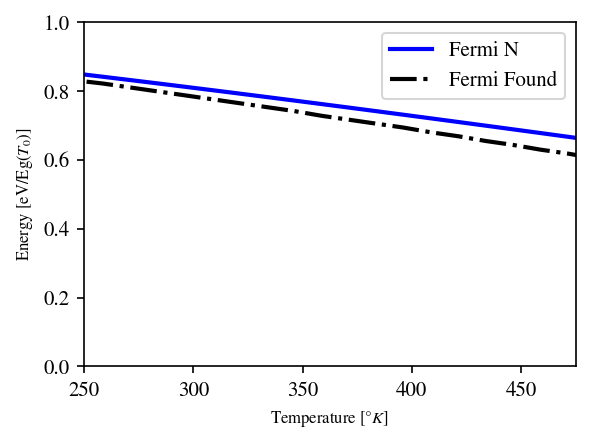
\includegraphics[width=0.6\textwidth]{fermi}
    %% Creator: Matplotlib, PGF backend
%%
%% To include the figure in your LaTeX document, write
%%   \input{<filename>.pgf}
%%
%% Make sure the required packages are loaded in your preamble
%%   \usepackage{pgf}
%%
%% Figures using additional raster images can only be included by \input if
%% they are in the same directory as the main LaTeX file. For loading figures
%% from other directories you can use the `import` package
%%   \usepackage{import}
%% and then include the figures with
%%   \import{<path to file>}{<filename>.pgf}
%%
%% Matplotlib used the following preamble
%%   \usepackage{gensymb}
%%   \usepackage[utf8x]{inputenc}
%%   \usepackage[T1]{fontenc}
%%
\begingroup%
\makeatletter%
\begin{pgfpicture}%
\pgfpathrectangle{\pgfpointorigin}{\pgfqpoint{3.930000in}{2.930000in}}%
\pgfusepath{use as bounding box, clip}%
\begin{pgfscope}%
\pgfsetbuttcap%
\pgfsetmiterjoin%
\definecolor{currentfill}{rgb}{1.000000,1.000000,1.000000}%
\pgfsetfillcolor{currentfill}%
\pgfsetlinewidth{0.000000pt}%
\definecolor{currentstroke}{rgb}{1.000000,1.000000,1.000000}%
\pgfsetstrokecolor{currentstroke}%
\pgfsetdash{}{0pt}%
\pgfpathmoveto{\pgfqpoint{0.000000in}{0.000000in}}%
\pgfpathlineto{\pgfqpoint{3.930000in}{0.000000in}}%
\pgfpathlineto{\pgfqpoint{3.930000in}{2.930000in}}%
\pgfpathlineto{\pgfqpoint{0.000000in}{2.930000in}}%
\pgfpathclose%
\pgfusepath{fill}%
\end{pgfscope}%
\begin{pgfscope}%
\pgfsetbuttcap%
\pgfsetmiterjoin%
\definecolor{currentfill}{rgb}{1.000000,1.000000,1.000000}%
\pgfsetfillcolor{currentfill}%
\pgfsetlinewidth{0.000000pt}%
\definecolor{currentstroke}{rgb}{0.000000,0.000000,0.000000}%
\pgfsetstrokecolor{currentstroke}%
\pgfsetstrokeopacity{0.000000}%
\pgfsetdash{}{0pt}%
\pgfpathmoveto{\pgfqpoint{0.555217in}{0.506458in}}%
\pgfpathlineto{\pgfqpoint{3.806667in}{0.506458in}}%
\pgfpathlineto{\pgfqpoint{3.806667in}{2.782172in}}%
\pgfpathlineto{\pgfqpoint{0.555217in}{2.782172in}}%
\pgfpathclose%
\pgfusepath{fill}%
\end{pgfscope}%
\begin{pgfscope}%
\pgfsetbuttcap%
\pgfsetroundjoin%
\definecolor{currentfill}{rgb}{0.000000,0.000000,0.000000}%
\pgfsetfillcolor{currentfill}%
\pgfsetlinewidth{0.803000pt}%
\definecolor{currentstroke}{rgb}{0.000000,0.000000,0.000000}%
\pgfsetstrokecolor{currentstroke}%
\pgfsetdash{}{0pt}%
\pgfsys@defobject{currentmarker}{\pgfqpoint{0.000000in}{-0.048611in}}{\pgfqpoint{0.000000in}{0.000000in}}{%
\pgfpathmoveto{\pgfqpoint{0.000000in}{0.000000in}}%
\pgfpathlineto{\pgfqpoint{0.000000in}{-0.048611in}}%
\pgfusepath{stroke,fill}%
}%
\begin{pgfscope}%
\pgfsys@transformshift{0.555217in}{0.506458in}%
\pgfsys@useobject{currentmarker}{}%
\end{pgfscope}%
\end{pgfscope}%
\begin{pgfscope}%
\pgftext[x=0.555217in,y=0.409236in,,top]{\fontsize{12.000000}{14.000000}\selectfont \(\displaystyle 250\)}%
\end{pgfscope}%
\begin{pgfscope}%
\pgfsetbuttcap%
\pgfsetroundjoin%
\definecolor{currentfill}{rgb}{0.000000,0.000000,0.000000}%
\pgfsetfillcolor{currentfill}%
\pgfsetlinewidth{0.803000pt}%
\definecolor{currentstroke}{rgb}{0.000000,0.000000,0.000000}%
\pgfsetstrokecolor{currentstroke}%
\pgfsetdash{}{0pt}%
\pgfsys@defobject{currentmarker}{\pgfqpoint{0.000000in}{-0.048611in}}{\pgfqpoint{0.000000in}{0.000000in}}{%
\pgfpathmoveto{\pgfqpoint{0.000000in}{0.000000in}}%
\pgfpathlineto{\pgfqpoint{0.000000in}{-0.048611in}}%
\pgfusepath{stroke,fill}%
}%
\begin{pgfscope}%
\pgfsys@transformshift{1.277761in}{0.506458in}%
\pgfsys@useobject{currentmarker}{}%
\end{pgfscope}%
\end{pgfscope}%
\begin{pgfscope}%
\pgftext[x=1.277761in,y=0.409236in,,top]{\fontsize{12.000000}{14.000000}\selectfont \(\displaystyle 300\)}%
\end{pgfscope}%
\begin{pgfscope}%
\pgfsetbuttcap%
\pgfsetroundjoin%
\definecolor{currentfill}{rgb}{0.000000,0.000000,0.000000}%
\pgfsetfillcolor{currentfill}%
\pgfsetlinewidth{0.803000pt}%
\definecolor{currentstroke}{rgb}{0.000000,0.000000,0.000000}%
\pgfsetstrokecolor{currentstroke}%
\pgfsetdash{}{0pt}%
\pgfsys@defobject{currentmarker}{\pgfqpoint{0.000000in}{-0.048611in}}{\pgfqpoint{0.000000in}{0.000000in}}{%
\pgfpathmoveto{\pgfqpoint{0.000000in}{0.000000in}}%
\pgfpathlineto{\pgfqpoint{0.000000in}{-0.048611in}}%
\pgfusepath{stroke,fill}%
}%
\begin{pgfscope}%
\pgfsys@transformshift{2.000306in}{0.506458in}%
\pgfsys@useobject{currentmarker}{}%
\end{pgfscope}%
\end{pgfscope}%
\begin{pgfscope}%
\pgftext[x=2.000306in,y=0.409236in,,top]{\fontsize{12.000000}{14.000000}\selectfont \(\displaystyle 350\)}%
\end{pgfscope}%
\begin{pgfscope}%
\pgfsetbuttcap%
\pgfsetroundjoin%
\definecolor{currentfill}{rgb}{0.000000,0.000000,0.000000}%
\pgfsetfillcolor{currentfill}%
\pgfsetlinewidth{0.803000pt}%
\definecolor{currentstroke}{rgb}{0.000000,0.000000,0.000000}%
\pgfsetstrokecolor{currentstroke}%
\pgfsetdash{}{0pt}%
\pgfsys@defobject{currentmarker}{\pgfqpoint{0.000000in}{-0.048611in}}{\pgfqpoint{0.000000in}{0.000000in}}{%
\pgfpathmoveto{\pgfqpoint{0.000000in}{0.000000in}}%
\pgfpathlineto{\pgfqpoint{0.000000in}{-0.048611in}}%
\pgfusepath{stroke,fill}%
}%
\begin{pgfscope}%
\pgfsys@transformshift{2.722850in}{0.506458in}%
\pgfsys@useobject{currentmarker}{}%
\end{pgfscope}%
\end{pgfscope}%
\begin{pgfscope}%
\pgftext[x=2.722850in,y=0.409236in,,top]{\fontsize{12.000000}{14.000000}\selectfont \(\displaystyle 400\)}%
\end{pgfscope}%
\begin{pgfscope}%
\pgfsetbuttcap%
\pgfsetroundjoin%
\definecolor{currentfill}{rgb}{0.000000,0.000000,0.000000}%
\pgfsetfillcolor{currentfill}%
\pgfsetlinewidth{0.803000pt}%
\definecolor{currentstroke}{rgb}{0.000000,0.000000,0.000000}%
\pgfsetstrokecolor{currentstroke}%
\pgfsetdash{}{0pt}%
\pgfsys@defobject{currentmarker}{\pgfqpoint{0.000000in}{-0.048611in}}{\pgfqpoint{0.000000in}{0.000000in}}{%
\pgfpathmoveto{\pgfqpoint{0.000000in}{0.000000in}}%
\pgfpathlineto{\pgfqpoint{0.000000in}{-0.048611in}}%
\pgfusepath{stroke,fill}%
}%
\begin{pgfscope}%
\pgfsys@transformshift{3.445394in}{0.506458in}%
\pgfsys@useobject{currentmarker}{}%
\end{pgfscope}%
\end{pgfscope}%
\begin{pgfscope}%
\pgftext[x=3.445394in,y=0.409236in,,top]{\fontsize{12.000000}{14.000000}\selectfont \(\displaystyle 450\)}%
\end{pgfscope}%
\begin{pgfscope}%
\pgftext[x=2.180942in,y=0.231025in,,top]{\fontsize{12.000000}{14.00000}\selectfont Temperature [K]}%
\end{pgfscope}%
\begin{pgfscope}%
\pgfsetbuttcap%
\pgfsetroundjoin%
\definecolor{currentfill}{rgb}{0.000000,0.000000,0.000000}%
\pgfsetfillcolor{currentfill}%
\pgfsetlinewidth{0.803000pt}%
\definecolor{currentstroke}{rgb}{0.000000,0.000000,0.000000}%
\pgfsetstrokecolor{currentstroke}%
\pgfsetdash{}{0pt}%
\pgfsys@defobject{currentmarker}{\pgfqpoint{-0.048611in}{0.000000in}}{\pgfqpoint{0.000000in}{0.000000in}}{%
\pgfpathmoveto{\pgfqpoint{0.000000in}{0.000000in}}%
\pgfpathlineto{\pgfqpoint{-0.048611in}{0.000000in}}%
\pgfusepath{stroke,fill}%
}%
\begin{pgfscope}%
\pgfsys@transformshift{0.555217in}{0.506458in}%
\pgfsys@useobject{currentmarker}{}%
\end{pgfscope}%
\end{pgfscope}%
\begin{pgfscope}%
\pgftext[x=0.280525in,y=0.458630in,left,base]{\fontsize{12.000000}{14.000000}\selectfont \(\displaystyle 0.0\)}%
\end{pgfscope}%
\begin{pgfscope}%
\pgfsetbuttcap%
\pgfsetroundjoin%
\definecolor{currentfill}{rgb}{0.000000,0.000000,0.000000}%
\pgfsetfillcolor{currentfill}%
\pgfsetlinewidth{0.803000pt}%
\definecolor{currentstroke}{rgb}{0.000000,0.000000,0.000000}%
\pgfsetstrokecolor{currentstroke}%
\pgfsetdash{}{0pt}%
\pgfsys@defobject{currentmarker}{\pgfqpoint{-0.048611in}{0.000000in}}{\pgfqpoint{0.000000in}{0.000000in}}{%
\pgfpathmoveto{\pgfqpoint{0.000000in}{0.000000in}}%
\pgfpathlineto{\pgfqpoint{-0.048611in}{0.000000in}}%
\pgfusepath{stroke,fill}%
}%
\begin{pgfscope}%
\pgfsys@transformshift{0.555217in}{0.961601in}%
\pgfsys@useobject{currentmarker}{}%
\end{pgfscope}%
\end{pgfscope}%
\begin{pgfscope}%
\pgftext[x=0.280525in,y=0.913773in,left,base]{\fontsize{12.000000}{14.000000}\selectfont \(\displaystyle 0.2\)}%
\end{pgfscope}%
\begin{pgfscope}%
\pgfsetbuttcap%
\pgfsetroundjoin%
\definecolor{currentfill}{rgb}{0.000000,0.000000,0.000000}%
\pgfsetfillcolor{currentfill}%
\pgfsetlinewidth{0.803000pt}%
\definecolor{currentstroke}{rgb}{0.000000,0.000000,0.000000}%
\pgfsetstrokecolor{currentstroke}%
\pgfsetdash{}{0pt}%
\pgfsys@defobject{currentmarker}{\pgfqpoint{-0.048611in}{0.000000in}}{\pgfqpoint{0.000000in}{0.000000in}}{%
\pgfpathmoveto{\pgfqpoint{0.000000in}{0.000000in}}%
\pgfpathlineto{\pgfqpoint{-0.048611in}{0.000000in}}%
\pgfusepath{stroke,fill}%
}%
\begin{pgfscope}%
\pgfsys@transformshift{0.555217in}{1.416744in}%
\pgfsys@useobject{currentmarker}{}%
\end{pgfscope}%
\end{pgfscope}%
\begin{pgfscope}%
\pgftext[x=0.280525in,y=1.368916in,left,base]{\fontsize{12.000000}{14.000000}\selectfont \(\displaystyle 0.4\)}%
\end{pgfscope}%
\begin{pgfscope}%
\pgfsetbuttcap%
\pgfsetroundjoin%
\definecolor{currentfill}{rgb}{0.000000,0.000000,0.000000}%
\pgfsetfillcolor{currentfill}%
\pgfsetlinewidth{0.803000pt}%
\definecolor{currentstroke}{rgb}{0.000000,0.000000,0.000000}%
\pgfsetstrokecolor{currentstroke}%
\pgfsetdash{}{0pt}%
\pgfsys@defobject{currentmarker}{\pgfqpoint{-0.048611in}{0.000000in}}{\pgfqpoint{0.000000in}{0.000000in}}{%
\pgfpathmoveto{\pgfqpoint{0.000000in}{0.000000in}}%
\pgfpathlineto{\pgfqpoint{-0.048611in}{0.000000in}}%
\pgfusepath{stroke,fill}%
}%
\begin{pgfscope}%
\pgfsys@transformshift{0.555217in}{1.871887in}%
\pgfsys@useobject{currentmarker}{}%
\end{pgfscope}%
\end{pgfscope}%
\begin{pgfscope}%
\pgftext[x=0.280525in,y=1.824059in,left,base]{\fontsize{12.000000}{14.000000}\selectfont \(\displaystyle 0.6\)}%
\end{pgfscope}%
\begin{pgfscope}%
\pgfsetbuttcap%
\pgfsetroundjoin%
\definecolor{currentfill}{rgb}{0.000000,0.000000,0.000000}%
\pgfsetfillcolor{currentfill}%
\pgfsetlinewidth{0.803000pt}%
\definecolor{currentstroke}{rgb}{0.000000,0.000000,0.000000}%
\pgfsetstrokecolor{currentstroke}%
\pgfsetdash{}{0pt}%
\pgfsys@defobject{currentmarker}{\pgfqpoint{-0.048611in}{0.000000in}}{\pgfqpoint{0.000000in}{0.000000in}}{%
\pgfpathmoveto{\pgfqpoint{0.000000in}{0.000000in}}%
\pgfpathlineto{\pgfqpoint{-0.048611in}{0.000000in}}%
\pgfusepath{stroke,fill}%
}%
\begin{pgfscope}%
\pgfsys@transformshift{0.555217in}{2.327029in}%
\pgfsys@useobject{currentmarker}{}%
\end{pgfscope}%
\end{pgfscope}%
\begin{pgfscope}%
\pgftext[x=0.280525in,y=2.279202in,left,base]{\fontsize{12.000000}{14.000000}\selectfont \(\displaystyle 0.8\)}%
\end{pgfscope}%
\begin{pgfscope}%
\pgfsetbuttcap%
\pgfsetroundjoin%
\definecolor{currentfill}{rgb}{0.000000,0.000000,0.000000}%
\pgfsetfillcolor{currentfill}%
\pgfsetlinewidth{0.803000pt}%
\definecolor{currentstroke}{rgb}{0.000000,0.000000,0.000000}%
\pgfsetstrokecolor{currentstroke}%
\pgfsetdash{}{0pt}%
\pgfsys@defobject{currentmarker}{\pgfqpoint{-0.048611in}{0.000000in}}{\pgfqpoint{0.000000in}{0.000000in}}{%
\pgfpathmoveto{\pgfqpoint{0.000000in}{0.000000in}}%
\pgfpathlineto{\pgfqpoint{-0.048611in}{0.000000in}}%
\pgfusepath{stroke,fill}%
}%
\begin{pgfscope}%
\pgfsys@transformshift{0.555217in}{2.782172in}%
\pgfsys@useobject{currentmarker}{}%
\end{pgfscope}%
\end{pgfscope}%
\begin{pgfscope}%
\pgftext[x=0.280525in,y=2.734344in,left,base]{\fontsize{12.000000}{14.000000}\selectfont \(\displaystyle 1.0\)}%
\end{pgfscope}%
\begin{pgfscope}%
\pgftext[x=0.224969in,y=1.644315in,,bottom,rotate=90.000000]{\fontsize{12.000000}{14.00000}\selectfont Energy [eV/Eg(\(\displaystyle T_0\))]}%
\end{pgfscope}%
\begin{pgfscope}%
\pgfpathrectangle{\pgfqpoint{0.555217in}{0.506458in}}{\pgfqpoint{3.251450in}{2.275714in}} %
\pgfusepath{clip}%
\pgfsetrectcap%
\pgfsetroundjoin%
\pgfsetlinewidth{2.007500pt}%
\definecolor{currentstroke}{rgb}{0.000000,0.000000,1.000000}%
\pgfsetstrokecolor{currentstroke}%
\pgfsetdash{}{0pt}%
\pgfpathmoveto{\pgfqpoint{0.548550in}{2.438024in}}%
\pgfpathlineto{\pgfqpoint{0.677393in}{2.422621in}}%
\pgfpathlineto{\pgfqpoint{0.858394in}{2.400749in}}%
\pgfpathlineto{\pgfqpoint{1.039395in}{2.378652in}}%
\pgfpathlineto{\pgfqpoint{1.220396in}{2.356341in}}%
\pgfpathlineto{\pgfqpoint{1.401397in}{2.333824in}}%
\pgfpathlineto{\pgfqpoint{1.582398in}{2.311110in}}%
\pgfpathlineto{\pgfqpoint{1.763399in}{2.288207in}}%
\pgfpathlineto{\pgfqpoint{1.944400in}{2.265121in}}%
\pgfpathlineto{\pgfqpoint{2.125401in}{2.241860in}}%
\pgfpathlineto{\pgfqpoint{2.306402in}{2.218429in}}%
\pgfpathlineto{\pgfqpoint{2.487403in}{2.194835in}}%
\pgfpathlineto{\pgfqpoint{2.668404in}{2.171082in}}%
\pgfpathlineto{\pgfqpoint{2.849405in}{2.147177in}}%
\pgfpathlineto{\pgfqpoint{3.030406in}{2.123125in}}%
\pgfpathlineto{\pgfqpoint{3.211407in}{2.098929in}}%
\pgfpathlineto{\pgfqpoint{3.392408in}{2.074595in}}%
\pgfpathlineto{\pgfqpoint{3.573409in}{2.050127in}}%
\pgfpathlineto{\pgfqpoint{3.754410in}{2.025531in}}%
\pgfpathlineto{\pgfqpoint{3.813333in}{2.017484in}}%
\pgfusepath{stroke}%
\end{pgfscope}%
\begin{pgfscope}%
\pgfpathrectangle{\pgfqpoint{0.555217in}{0.506458in}}{\pgfqpoint{3.251450in}{2.275714in}} %
\pgfusepath{clip}%
\pgfsetbuttcap%
\pgfsetroundjoin%
\pgfsetlinewidth{2.007500pt}%
\definecolor{currentstroke}{rgb}{0.000000,0.000000,0.000000}%
\pgfsetstrokecolor{currentstroke}%
\pgfsetdash{{12.800000pt}{3.200000pt}{2.000000pt}{3.200000pt}}{0.000000pt}%
\pgfpathmoveto{\pgfqpoint{0.548550in}{2.392610in}}%
\pgfpathlineto{\pgfqpoint{0.677393in}{2.377780in}}%
\pgfpathlineto{\pgfqpoint{0.858394in}{2.351737in}}%
\pgfpathlineto{\pgfqpoint{1.039395in}{2.325695in}}%
\pgfpathlineto{\pgfqpoint{1.220396in}{2.299652in}}%
\pgfpathlineto{\pgfqpoint{1.401397in}{2.273610in}}%
\pgfpathlineto{\pgfqpoint{1.582398in}{2.247567in}}%
\pgfpathlineto{\pgfqpoint{1.763399in}{2.221524in}}%
\pgfpathlineto{\pgfqpoint{1.944400in}{2.195482in}}%
\pgfpathlineto{\pgfqpoint{2.125401in}{2.164231in}}%
\pgfpathlineto{\pgfqpoint{2.306402in}{2.138188in}}%
\pgfpathlineto{\pgfqpoint{2.487403in}{2.112146in}}%
\pgfpathlineto{\pgfqpoint{2.668404in}{2.086103in}}%
\pgfpathlineto{\pgfqpoint{2.849405in}{2.054852in}}%
\pgfpathlineto{\pgfqpoint{3.030406in}{2.028809in}}%
\pgfpathlineto{\pgfqpoint{3.211407in}{1.997558in}}%
\pgfpathlineto{\pgfqpoint{3.392408in}{1.971516in}}%
\pgfpathlineto{\pgfqpoint{3.573409in}{1.940265in}}%
\pgfpathlineto{\pgfqpoint{3.754410in}{1.914222in}}%
\pgfpathlineto{\pgfqpoint{3.813333in}{1.904049in}}%
\pgfusepath{stroke}%
\end{pgfscope}%
\begin{pgfscope}%
\pgfsetrectcap%
\pgfsetmiterjoin%
\pgfsetlinewidth{0.803000pt}%
\definecolor{currentstroke}{rgb}{0.000000,0.000000,0.000000}%
\pgfsetstrokecolor{currentstroke}%
\pgfsetdash{}{0pt}%
\pgfpathmoveto{\pgfqpoint{0.555217in}{0.506458in}}%
\pgfpathlineto{\pgfqpoint{0.555217in}{2.782172in}}%
\pgfusepath{stroke}%
\end{pgfscope}%
\begin{pgfscope}%
\pgfsetrectcap%
\pgfsetmiterjoin%
\pgfsetlinewidth{0.803000pt}%
\definecolor{currentstroke}{rgb}{0.000000,0.000000,0.000000}%
\pgfsetstrokecolor{currentstroke}%
\pgfsetdash{}{0pt}%
\pgfpathmoveto{\pgfqpoint{3.806667in}{0.506458in}}%
\pgfpathlineto{\pgfqpoint{3.806667in}{2.782172in}}%
\pgfusepath{stroke}%
\end{pgfscope}%
\begin{pgfscope}%
\pgfsetrectcap%
\pgfsetmiterjoin%
\pgfsetlinewidth{0.803000pt}%
\definecolor{currentstroke}{rgb}{0.000000,0.000000,0.000000}%
\pgfsetstrokecolor{currentstroke}%
\pgfsetdash{}{0pt}%
\pgfpathmoveto{\pgfqpoint{0.555217in}{0.506458in}}%
\pgfpathlineto{\pgfqpoint{3.806667in}{0.506458in}}%
\pgfusepath{stroke}%
\end{pgfscope}%
\begin{pgfscope}%
\pgfsetrectcap%
\pgfsetmiterjoin%
\pgfsetlinewidth{0.803000pt}%
\definecolor{currentstroke}{rgb}{0.000000,0.000000,0.000000}%
\pgfsetstrokecolor{currentstroke}%
\pgfsetdash{}{0pt}%
\pgfpathmoveto{\pgfqpoint{0.555217in}{2.782172in}}%
\pgfpathlineto{\pgfqpoint{3.806667in}{2.782172in}}%
\pgfusepath{stroke}%
\end{pgfscope}%
\begin{pgfscope}%
\pgfsetbuttcap%
\pgfsetmiterjoin%
\definecolor{currentfill}{rgb}{1.000000,1.000000,1.000000}%
\pgfsetfillcolor{currentfill}%
\pgfsetfillopacity{0.800000}%
\pgfsetlinewidth{1.003750pt}%
\definecolor{currentstroke}{rgb}{0.800000,0.800000,0.800000}%
\pgfsetstrokecolor{currentstroke}%
\pgfsetstrokeopacity{0.800000}%
\pgfsetdash{}{0pt}%
\pgfpathmoveto{\pgfqpoint{2.489341in}{2.283729in}}%
\pgfpathlineto{\pgfqpoint{3.709444in}{2.283729in}}%
\pgfpathquadraticcurveto{\pgfqpoint{3.737222in}{2.283729in}}{\pgfqpoint{3.737222in}{2.311506in}}%
\pgfpathlineto{\pgfqpoint{3.737222in}{2.684950in}}%
\pgfpathquadraticcurveto{\pgfqpoint{3.737222in}{2.712728in}}{\pgfqpoint{3.709444in}{2.712728in}}%
\pgfpathlineto{\pgfqpoint{2.489341in}{2.712728in}}%
\pgfpathquadraticcurveto{\pgfqpoint{2.461563in}{2.712728in}}{\pgfqpoint{2.461563in}{2.684950in}}%
\pgfpathlineto{\pgfqpoint{2.461563in}{2.311506in}}%
\pgfpathquadraticcurveto{\pgfqpoint{2.461563in}{2.283729in}}{\pgfqpoint{2.489341in}{2.283729in}}%
\pgfpathclose%
\pgfusepath{stroke,fill}%
\end{pgfscope}%
\begin{pgfscope}%
\pgfsetrectcap%
\pgfsetroundjoin%
\pgfsetlinewidth{2.007500pt}%
\definecolor{currentstroke}{rgb}{0.000000,0.000000,1.000000}%
\pgfsetstrokecolor{currentstroke}%
\pgfsetdash{}{0pt}%
\pgfpathmoveto{\pgfqpoint{2.517118in}{2.608561in}}%
\pgfpathlineto{\pgfqpoint{2.794896in}{2.608561in}}%
\pgfusepath{stroke}%
\end{pgfscope}%
\begin{pgfscope}%
\pgftext[x=2.906007in,y=2.559950in,left,base]{\fontsize{10.000000}{12.000000}\selectfont Fermi N}%
\end{pgfscope}%
\begin{pgfscope}%
\pgfsetbuttcap%
\pgfsetroundjoin%
\pgfsetlinewidth{2.007500pt}%
\definecolor{currentstroke}{rgb}{0.000000,0.000000,0.000000}%
\pgfsetstrokecolor{currentstroke}%
\pgfsetdash{{12.800000pt}{3.200000pt}{2.000000pt}{3.200000pt}}{0.000000pt}%
\pgfpathmoveto{\pgfqpoint{2.517118in}{2.414895in}}%
\pgfpathlineto{\pgfqpoint{2.794896in}{2.414895in}}%
\pgfusepath{stroke}%
\end{pgfscope}%
\begin{pgfscope}%
\pgftext[x=2.906007in,y=2.366284in,left,base]{\fontsize{10.000000}{12.000000}\selectfont Fermi Found}%
\end{pgfscope}%
\end{pgfpicture}%
\makeatother%
\endgroup%

    \caption{Fermi energy normalized over the temperature range of interest without (b-) and with (k-) impurities in the substrate}
    \label{fig:electron_fermi_si}
\end{figure}

For practical design, the variation over temperature of the threshold voltage is modelled in the BSIM model as:

\begin{equation}
V_{th}(T) = V_{th0} + \alpha (T - T_0)
\end{equation}
where \(\alpha = \frac{KT1}{T_0}+\frac{KT1.L}{L_{eff} T_0}+\frac{KT2 V_{bseff}}{T_0}\) represents the linearised variation coefficient with respect of the temperature, depicted by \figurename~\ref{fig:vth_nel}. \figurename~\ref{fig:vth_nel}a represents both the threshold voltage decreasing with the temperature (solid line) and the thermal behaviour for a lot under a 3\(\sigma \) process variation delimited by the shaded area around the average. The slope depends on the transistor channel length L and the bulk-source voltage applied. For a voltage \(V_{bs} = 0 \) as done in the \figurename~\ref{fig:vth_nel_L}b, the bigger the channel length is, less sensitive is the threshold voltage. This offer the possibility to the designer to adjust the threshold voltage temperature sensitivity by either decreasing the transistor channel length or body biasing~\cite{Kumar2008}.

\begin{figure}[!ht]
    \centering
    \begin{subfigure}[b]{0.48\textwidth}
        %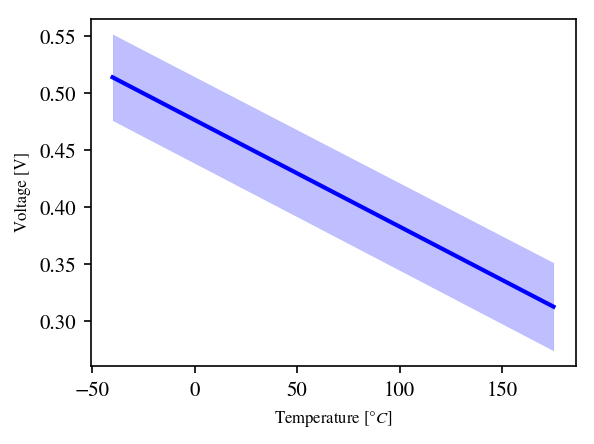
\includegraphics[width=\textwidth]{vth_nel}
        \resizebox {\textwidth} {!} { 
            %% Creator: Matplotlib, PGF backend
%%
%% To include the figure in your LaTeX document, write
%%   \input{<filename>.pgf}
%%
%% Make sure the required packages are loaded in your preamble
%%   \usepackage{pgf}
%%
%% Figures using additional raster images can only be included by \input if
%% they are in the same directory as the main LaTeX file. For loading figures
%% from other directories you can use the `import` package
%%   \usepackage{import}
%% and then include the figures with
%%   \import{<path to file>}{<filename>.pgf}
%%
%% Matplotlib used the following preamble
%%   \usepackage{gensymb}
%%   \usepackage[utf8x]{inputenc}
%%   \usepackage[T1]{fontenc}
%%
\begingroup%
\makeatletter%
\begin{pgfpicture}%
\pgfpathrectangle{\pgfpointorigin}{\pgfqpoint{3.840000in}{2.840000in}}%
\pgfusepath{use as bounding box, clip}%
\begin{pgfscope}%
\pgfsetbuttcap%
\pgfsetmiterjoin%
\definecolor{currentfill}{rgb}{1.000000,1.000000,1.000000}%
\pgfsetfillcolor{currentfill}%
\pgfsetlinewidth{0.000000pt}%
\definecolor{currentstroke}{rgb}{1.000000,1.000000,1.000000}%
\pgfsetstrokecolor{currentstroke}%
\pgfsetdash{}{0pt}%
\pgfpathmoveto{\pgfqpoint{0.000000in}{0.000000in}}%
\pgfpathlineto{\pgfqpoint{3.840000in}{0.000000in}}%
\pgfpathlineto{\pgfqpoint{3.840000in}{2.840000in}}%
\pgfpathlineto{\pgfqpoint{0.000000in}{2.840000in}}%
\pgfpathclose%
\pgfusepath{fill}%
\end{pgfscope}%
\begin{pgfscope}%
\pgfsetbuttcap%
\pgfsetmiterjoin%
\definecolor{currentfill}{rgb}{1.000000,1.000000,1.000000}%
\pgfsetfillcolor{currentfill}%
\pgfsetlinewidth{0.000000pt}%
\definecolor{currentstroke}{rgb}{0.000000,0.000000,0.000000}%
\pgfsetstrokecolor{currentstroke}%
\pgfsetstrokeopacity{0.000000}%
\pgfsetdash{}{0pt}%
\pgfpathmoveto{\pgfqpoint{0.669632in}{0.596026in}}%
\pgfpathlineto{\pgfqpoint{3.716667in}{0.596026in}}%
\pgfpathlineto{\pgfqpoint{3.716667in}{2.716667in}}%
\pgfpathlineto{\pgfqpoint{0.669632in}{2.716667in}}%
\pgfpathclose%
\pgfusepath{fill}%
\end{pgfscope}%
\begin{pgfscope}%
\pgfpathrectangle{\pgfqpoint{0.669632in}{0.596026in}}{\pgfqpoint{3.047035in}{2.120641in}} %
\pgfusepath{clip}%
\pgfsetbuttcap%
\pgfsetroundjoin%
\definecolor{currentfill}{rgb}{0.000000,0.000000,1.000000}%
\pgfsetfillcolor{currentfill}%
\pgfsetfillopacity{0.250000}%
\pgfsetlinewidth{0.100375pt}%
\definecolor{currentstroke}{rgb}{0.000000,0.000000,1.000000}%
\pgfsetstrokecolor{currentstroke}%
\pgfsetstrokeopacity{0.250000}%
\pgfsetdash{}{0pt}%
\pgfpathmoveto{\pgfqpoint{0.808134in}{2.620274in}}%
\pgfpathlineto{\pgfqpoint{0.808134in}{2.096052in}}%
\pgfpathlineto{\pgfqpoint{1.001392in}{1.998114in}}%
\pgfpathlineto{\pgfqpoint{1.323488in}{1.835296in}}%
\pgfpathlineto{\pgfqpoint{1.671353in}{1.659042in}}%
\pgfpathlineto{\pgfqpoint{1.967682in}{1.508987in}}%
\pgfpathlineto{\pgfqpoint{2.289778in}{1.345787in}}%
\pgfpathlineto{\pgfqpoint{2.418617in}{1.280326in}}%
\pgfpathlineto{\pgfqpoint{2.611875in}{1.182633in}}%
\pgfpathlineto{\pgfqpoint{2.933972in}{1.019122in}}%
\pgfpathlineto{\pgfqpoint{3.256068in}{0.855719in}}%
\pgfpathlineto{\pgfqpoint{3.578165in}{0.692419in}}%
\pgfpathlineto{\pgfqpoint{3.578165in}{1.227117in}}%
\pgfpathlineto{\pgfqpoint{3.578165in}{1.227117in}}%
\pgfpathlineto{\pgfqpoint{3.256068in}{1.388933in}}%
\pgfpathlineto{\pgfqpoint{2.933972in}{1.550813in}}%
\pgfpathlineto{\pgfqpoint{2.611875in}{1.712502in}}%
\pgfpathlineto{\pgfqpoint{2.418617in}{1.809806in}}%
\pgfpathlineto{\pgfqpoint{2.289778in}{1.874491in}}%
\pgfpathlineto{\pgfqpoint{1.967682in}{2.036547in}}%
\pgfpathlineto{\pgfqpoint{1.671353in}{2.185618in}}%
\pgfpathlineto{\pgfqpoint{1.323488in}{2.360694in}}%
\pgfpathlineto{\pgfqpoint{1.001392in}{2.523020in}}%
\pgfpathlineto{\pgfqpoint{0.808134in}{2.620274in}}%
\pgfpathclose%
\pgfusepath{stroke,fill}%
\end{pgfscope}%
\begin{pgfscope}%
\pgfsetbuttcap%
\pgfsetroundjoin%
\definecolor{currentfill}{rgb}{0.000000,0.000000,0.000000}%
\pgfsetfillcolor{currentfill}%
\pgfsetlinewidth{0.803000pt}%
\definecolor{currentstroke}{rgb}{0.000000,0.000000,0.000000}%
\pgfsetstrokecolor{currentstroke}%
\pgfsetdash{}{0pt}%
\pgfsys@defobject{currentmarker}{\pgfqpoint{0.000000in}{-0.048611in}}{\pgfqpoint{0.000000in}{0.000000in}}{%
\pgfpathmoveto{\pgfqpoint{0.000000in}{0.000000in}}%
\pgfpathlineto{\pgfqpoint{0.000000in}{-0.048611in}}%
\pgfusepath{stroke,fill}%
}%
\begin{pgfscope}%
\pgfsys@transformshift{0.679295in}{0.596026in}%
\pgfsys@useobject{currentmarker}{}%
\end{pgfscope}%
\end{pgfscope}%
\begin{pgfscope}%
\pgftext[x=0.679295in,y=0.498804in,,top]{\fontsize{14.000000}{16.800000}\selectfont \(\displaystyle -50\)}%
\end{pgfscope}%
\begin{pgfscope}%
\pgfsetbuttcap%
\pgfsetroundjoin%
\definecolor{currentfill}{rgb}{0.000000,0.000000,0.000000}%
\pgfsetfillcolor{currentfill}%
\pgfsetlinewidth{0.803000pt}%
\definecolor{currentstroke}{rgb}{0.000000,0.000000,0.000000}%
\pgfsetstrokecolor{currentstroke}%
\pgfsetdash{}{0pt}%
\pgfsys@defobject{currentmarker}{\pgfqpoint{0.000000in}{-0.048611in}}{\pgfqpoint{0.000000in}{0.000000in}}{%
\pgfpathmoveto{\pgfqpoint{0.000000in}{0.000000in}}%
\pgfpathlineto{\pgfqpoint{0.000000in}{-0.048611in}}%
\pgfusepath{stroke,fill}%
}%
\begin{pgfscope}%
\pgfsys@transformshift{1.323488in}{0.596026in}%
\pgfsys@useobject{currentmarker}{}%
\end{pgfscope}%
\end{pgfscope}%
\begin{pgfscope}%
\pgftext[x=1.323488in,y=0.498804in,,top]{\fontsize{14.000000}{16.800000}\selectfont \(\displaystyle 0\)}%
\end{pgfscope}%
\begin{pgfscope}%
\pgfsetbuttcap%
\pgfsetroundjoin%
\definecolor{currentfill}{rgb}{0.000000,0.000000,0.000000}%
\pgfsetfillcolor{currentfill}%
\pgfsetlinewidth{0.803000pt}%
\definecolor{currentstroke}{rgb}{0.000000,0.000000,0.000000}%
\pgfsetstrokecolor{currentstroke}%
\pgfsetdash{}{0pt}%
\pgfsys@defobject{currentmarker}{\pgfqpoint{0.000000in}{-0.048611in}}{\pgfqpoint{0.000000in}{0.000000in}}{%
\pgfpathmoveto{\pgfqpoint{0.000000in}{0.000000in}}%
\pgfpathlineto{\pgfqpoint{0.000000in}{-0.048611in}}%
\pgfusepath{stroke,fill}%
}%
\begin{pgfscope}%
\pgfsys@transformshift{1.967682in}{0.596026in}%
\pgfsys@useobject{currentmarker}{}%
\end{pgfscope}%
\end{pgfscope}%
\begin{pgfscope}%
\pgftext[x=1.967682in,y=0.498804in,,top]{\fontsize{14.000000}{16.800000}\selectfont \(\displaystyle 50\)}%
\end{pgfscope}%
\begin{pgfscope}%
\pgfsetbuttcap%
\pgfsetroundjoin%
\definecolor{currentfill}{rgb}{0.000000,0.000000,0.000000}%
\pgfsetfillcolor{currentfill}%
\pgfsetlinewidth{0.803000pt}%
\definecolor{currentstroke}{rgb}{0.000000,0.000000,0.000000}%
\pgfsetstrokecolor{currentstroke}%
\pgfsetdash{}{0pt}%
\pgfsys@defobject{currentmarker}{\pgfqpoint{0.000000in}{-0.048611in}}{\pgfqpoint{0.000000in}{0.000000in}}{%
\pgfpathmoveto{\pgfqpoint{0.000000in}{0.000000in}}%
\pgfpathlineto{\pgfqpoint{0.000000in}{-0.048611in}}%
\pgfusepath{stroke,fill}%
}%
\begin{pgfscope}%
\pgfsys@transformshift{2.611875in}{0.596026in}%
\pgfsys@useobject{currentmarker}{}%
\end{pgfscope}%
\end{pgfscope}%
\begin{pgfscope}%
\pgftext[x=2.611875in,y=0.498804in,,top]{\fontsize{14.000000}{16.800000}\selectfont \(\displaystyle 100\)}%
\end{pgfscope}%
\begin{pgfscope}%
\pgfsetbuttcap%
\pgfsetroundjoin%
\definecolor{currentfill}{rgb}{0.000000,0.000000,0.000000}%
\pgfsetfillcolor{currentfill}%
\pgfsetlinewidth{0.803000pt}%
\definecolor{currentstroke}{rgb}{0.000000,0.000000,0.000000}%
\pgfsetstrokecolor{currentstroke}%
\pgfsetdash{}{0pt}%
\pgfsys@defobject{currentmarker}{\pgfqpoint{0.000000in}{-0.048611in}}{\pgfqpoint{0.000000in}{0.000000in}}{%
\pgfpathmoveto{\pgfqpoint{0.000000in}{0.000000in}}%
\pgfpathlineto{\pgfqpoint{0.000000in}{-0.048611in}}%
\pgfusepath{stroke,fill}%
}%
\begin{pgfscope}%
\pgfsys@transformshift{3.256068in}{0.596026in}%
\pgfsys@useobject{currentmarker}{}%
\end{pgfscope}%
\end{pgfscope}%
\begin{pgfscope}%
\pgftext[x=3.256068in,y=0.498804in,,top]{\fontsize{14.000000}{16.800000}\selectfont \(\displaystyle 150\)}%
\end{pgfscope}%
\begin{pgfscope}%
\pgftext[x=2.193149in,y=0.266626in,,top]{\fontsize{12.000000}{14.400000}\selectfont Temperature [\(\displaystyle \degree C\)]}%
\end{pgfscope}%
\begin{pgfscope}%
\pgfsetbuttcap%
\pgfsetroundjoin%
\definecolor{currentfill}{rgb}{0.000000,0.000000,0.000000}%
\pgfsetfillcolor{currentfill}%
\pgfsetlinewidth{0.803000pt}%
\definecolor{currentstroke}{rgb}{0.000000,0.000000,0.000000}%
\pgfsetstrokecolor{currentstroke}%
\pgfsetdash{}{0pt}%
\pgfsys@defobject{currentmarker}{\pgfqpoint{-0.048611in}{0.000000in}}{\pgfqpoint{0.000000in}{0.000000in}}{%
\pgfpathmoveto{\pgfqpoint{0.000000in}{0.000000in}}%
\pgfpathlineto{\pgfqpoint{-0.048611in}{0.000000in}}%
\pgfusepath{stroke,fill}%
}%
\begin{pgfscope}%
\pgfsys@transformshift{0.669632in}{0.871136in}%
\pgfsys@useobject{currentmarker}{}%
\end{pgfscope}%
\end{pgfscope}%
\begin{pgfscope}%
\pgftext[x=0.322182in,y=0.802270in,left,base]{\fontsize{14.000000}{16.800000}\selectfont \(\displaystyle 0.3\)}%
\end{pgfscope}%
\begin{pgfscope}%
\pgfsetbuttcap%
\pgfsetroundjoin%
\definecolor{currentfill}{rgb}{0.000000,0.000000,0.000000}%
\pgfsetfillcolor{currentfill}%
\pgfsetlinewidth{0.803000pt}%
\definecolor{currentstroke}{rgb}{0.000000,0.000000,0.000000}%
\pgfsetstrokecolor{currentstroke}%
\pgfsetdash{}{0pt}%
\pgfsys@defobject{currentmarker}{\pgfqpoint{-0.048611in}{0.000000in}}{\pgfqpoint{0.000000in}{0.000000in}}{%
\pgfpathmoveto{\pgfqpoint{0.000000in}{0.000000in}}%
\pgfpathlineto{\pgfqpoint{-0.048611in}{0.000000in}}%
\pgfusepath{stroke,fill}%
}%
\begin{pgfscope}%
\pgfsys@transformshift{0.669632in}{1.566067in}%
\pgfsys@useobject{currentmarker}{}%
\end{pgfscope}%
\end{pgfscope}%
\begin{pgfscope}%
\pgftext[x=0.322182in,y=1.497201in,left,base]{\fontsize{14.000000}{16.800000}\selectfont \(\displaystyle 0.4\)}%
\end{pgfscope}%
\begin{pgfscope}%
\pgfsetbuttcap%
\pgfsetroundjoin%
\definecolor{currentfill}{rgb}{0.000000,0.000000,0.000000}%
\pgfsetfillcolor{currentfill}%
\pgfsetlinewidth{0.803000pt}%
\definecolor{currentstroke}{rgb}{0.000000,0.000000,0.000000}%
\pgfsetstrokecolor{currentstroke}%
\pgfsetdash{}{0pt}%
\pgfsys@defobject{currentmarker}{\pgfqpoint{-0.048611in}{0.000000in}}{\pgfqpoint{0.000000in}{0.000000in}}{%
\pgfpathmoveto{\pgfqpoint{0.000000in}{0.000000in}}%
\pgfpathlineto{\pgfqpoint{-0.048611in}{0.000000in}}%
\pgfusepath{stroke,fill}%
}%
\begin{pgfscope}%
\pgfsys@transformshift{0.669632in}{2.260998in}%
\pgfsys@useobject{currentmarker}{}%
\end{pgfscope}%
\end{pgfscope}%
\begin{pgfscope}%
\pgftext[x=0.322182in,y=2.192132in,left,base]{\fontsize{14.000000}{16.800000}\selectfont \(\displaystyle 0.5\)}%
\end{pgfscope}%
\begin{pgfscope}%
\pgftext[x=0.266626in,y=1.656346in,,bottom,rotate=90.000000]{\fontsize{12.000000}{14.400000}\selectfont Voltage [V]}%
\end{pgfscope}%
\begin{pgfscope}%
\pgfpathrectangle{\pgfqpoint{0.669632in}{0.596026in}}{\pgfqpoint{3.047035in}{2.120641in}} %
\pgfusepath{clip}%
\pgfsetrectcap%
\pgfsetroundjoin%
\pgfsetlinewidth{2.007500pt}%
\definecolor{currentstroke}{rgb}{0.000000,0.000000,1.000000}%
\pgfsetstrokecolor{currentstroke}%
\pgfsetdash{}{0pt}%
\pgfpathmoveto{\pgfqpoint{0.808134in}{2.358163in}}%
\pgfpathlineto{\pgfqpoint{1.001392in}{2.260567in}}%
\pgfpathlineto{\pgfqpoint{1.323488in}{2.097995in}}%
\pgfpathlineto{\pgfqpoint{1.671353in}{1.922330in}}%
\pgfpathlineto{\pgfqpoint{1.967682in}{1.772767in}}%
\pgfpathlineto{\pgfqpoint{2.289778in}{1.610139in}}%
\pgfpathlineto{\pgfqpoint{2.418617in}{1.545066in}}%
\pgfpathlineto{\pgfqpoint{2.611875in}{1.447567in}}%
\pgfpathlineto{\pgfqpoint{2.933972in}{1.284967in}}%
\pgfpathlineto{\pgfqpoint{3.256068in}{1.122326in}}%
\pgfpathlineto{\pgfqpoint{3.578165in}{0.959768in}}%
\pgfusepath{stroke}%
\end{pgfscope}%
\begin{pgfscope}%
\pgfsetrectcap%
\pgfsetmiterjoin%
\pgfsetlinewidth{0.803000pt}%
\definecolor{currentstroke}{rgb}{0.000000,0.000000,0.000000}%
\pgfsetstrokecolor{currentstroke}%
\pgfsetdash{}{0pt}%
\pgfpathmoveto{\pgfqpoint{0.669632in}{0.596026in}}%
\pgfpathlineto{\pgfqpoint{0.669632in}{2.716667in}}%
\pgfusepath{stroke}%
\end{pgfscope}%
\begin{pgfscope}%
\pgfsetrectcap%
\pgfsetmiterjoin%
\pgfsetlinewidth{0.803000pt}%
\definecolor{currentstroke}{rgb}{0.000000,0.000000,0.000000}%
\pgfsetstrokecolor{currentstroke}%
\pgfsetdash{}{0pt}%
\pgfpathmoveto{\pgfqpoint{3.716667in}{0.596026in}}%
\pgfpathlineto{\pgfqpoint{3.716667in}{2.716667in}}%
\pgfusepath{stroke}%
\end{pgfscope}%
\begin{pgfscope}%
\pgfsetrectcap%
\pgfsetmiterjoin%
\pgfsetlinewidth{0.803000pt}%
\definecolor{currentstroke}{rgb}{0.000000,0.000000,0.000000}%
\pgfsetstrokecolor{currentstroke}%
\pgfsetdash{}{0pt}%
\pgfpathmoveto{\pgfqpoint{0.669632in}{0.596026in}}%
\pgfpathlineto{\pgfqpoint{3.716667in}{0.596026in}}%
\pgfusepath{stroke}%
\end{pgfscope}%
\begin{pgfscope}%
\pgfsetrectcap%
\pgfsetmiterjoin%
\pgfsetlinewidth{0.803000pt}%
\definecolor{currentstroke}{rgb}{0.000000,0.000000,0.000000}%
\pgfsetstrokecolor{currentstroke}%
\pgfsetdash{}{0pt}%
\pgfpathmoveto{\pgfqpoint{0.669632in}{2.716667in}}%
\pgfpathlineto{\pgfqpoint{3.716667in}{2.716667in}}%
\pgfusepath{stroke}%
\end{pgfscope}%
\end{pgfpicture}%
\makeatother%
\endgroup%

        }
        \subcaption{average and \(\pm 3\sigma \) process variation range}
    \end{subfigure}
    \begin{subfigure}[b]{0.48\textwidth}
        %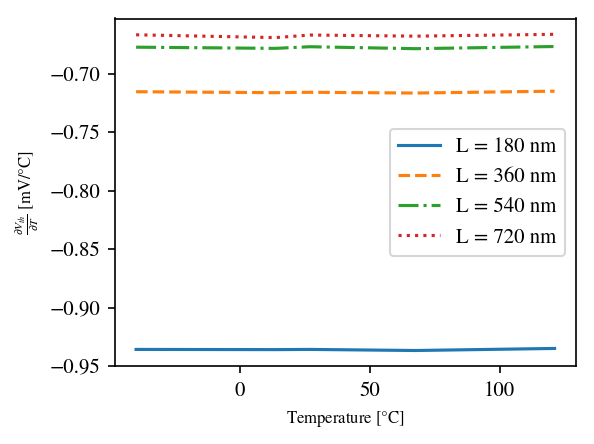
\includegraphics[width=\textwidth]{vth_nel_T}
        \resizebox {\textwidth} {!} { 
            %% Creator: Matplotlib, PGF backend
%%
%% To include the figure in your LaTeX document, write
%%   \input{<filename>.pgf}
%%
%% Make sure the required packages are loaded in your preamble
%%   \usepackage{pgf}
%%
%% Figures using additional raster images can only be included by \input if
%% they are in the same directory as the main LaTeX file. For loading figures
%% from other directories you can use the `import` package
%%   \usepackage{import}
%% and then include the figures with
%%   \import{<path to file>}{<filename>.pgf}
%%
%% Matplotlib used the following preamble
%%   \usepackage{gensymb}
%%   \usepackage[utf8x]{inputenc}
%%   \usepackage[T1]{fontenc}
%%
\begingroup%
\makeatletter%
\begin{pgfpicture}%
\pgfpathrectangle{\pgfpointorigin}{\pgfqpoint{3.840000in}{2.840000in}}%
\pgfusepath{use as bounding box, clip}%
\begin{pgfscope}%
\pgfsetbuttcap%
\pgfsetmiterjoin%
\definecolor{currentfill}{rgb}{1.000000,1.000000,1.000000}%
\pgfsetfillcolor{currentfill}%
\pgfsetlinewidth{0.000000pt}%
\definecolor{currentstroke}{rgb}{1.000000,1.000000,1.000000}%
\pgfsetstrokecolor{currentstroke}%
\pgfsetdash{}{0pt}%
\pgfpathmoveto{\pgfqpoint{0.000000in}{0.000000in}}%
\pgfpathlineto{\pgfqpoint{3.840000in}{0.000000in}}%
\pgfpathlineto{\pgfqpoint{3.840000in}{2.840000in}}%
\pgfpathlineto{\pgfqpoint{0.000000in}{2.840000in}}%
\pgfpathclose%
\pgfusepath{fill}%
\end{pgfscope}%
\begin{pgfscope}%
\pgfsetbuttcap%
\pgfsetmiterjoin%
\definecolor{currentfill}{rgb}{1.000000,1.000000,1.000000}%
\pgfsetfillcolor{currentfill}%
\pgfsetlinewidth{0.000000pt}%
\definecolor{currentstroke}{rgb}{0.000000,0.000000,0.000000}%
\pgfsetstrokecolor{currentstroke}%
\pgfsetstrokeopacity{0.000000}%
\pgfsetdash{}{0pt}%
\pgfpathmoveto{\pgfqpoint{1.001379in}{0.596026in}}%
\pgfpathlineto{\pgfqpoint{3.716667in}{0.596026in}}%
\pgfpathlineto{\pgfqpoint{3.716667in}{2.716667in}}%
\pgfpathlineto{\pgfqpoint{1.001379in}{2.716667in}}%
\pgfpathclose%
\pgfusepath{fill}%
\end{pgfscope}%
\begin{pgfscope}%
\pgfsetbuttcap%
\pgfsetroundjoin%
\definecolor{currentfill}{rgb}{0.000000,0.000000,0.000000}%
\pgfsetfillcolor{currentfill}%
\pgfsetlinewidth{0.803000pt}%
\definecolor{currentstroke}{rgb}{0.000000,0.000000,0.000000}%
\pgfsetstrokecolor{currentstroke}%
\pgfsetdash{}{0pt}%
\pgfsys@defobject{currentmarker}{\pgfqpoint{0.000000in}{-0.048611in}}{\pgfqpoint{0.000000in}{0.000000in}}{%
\pgfpathmoveto{\pgfqpoint{0.000000in}{0.000000in}}%
\pgfpathlineto{\pgfqpoint{0.000000in}{-0.048611in}}%
\pgfusepath{stroke,fill}%
}%
\begin{pgfscope}%
\pgfsys@transformshift{1.737318in}{0.596026in}%
\pgfsys@useobject{currentmarker}{}%
\end{pgfscope}%
\end{pgfscope}%
\begin{pgfscope}%
\pgftext[x=1.737318in,y=0.498804in,,top]{\fontsize{14.000000}{16.800000}\selectfont \(\displaystyle 0\)}%
\end{pgfscope}%
\begin{pgfscope}%
\pgfsetbuttcap%
\pgfsetroundjoin%
\definecolor{currentfill}{rgb}{0.000000,0.000000,0.000000}%
\pgfsetfillcolor{currentfill}%
\pgfsetlinewidth{0.803000pt}%
\definecolor{currentstroke}{rgb}{0.000000,0.000000,0.000000}%
\pgfsetstrokecolor{currentstroke}%
\pgfsetdash{}{0pt}%
\pgfsys@defobject{currentmarker}{\pgfqpoint{0.000000in}{-0.048611in}}{\pgfqpoint{0.000000in}{0.000000in}}{%
\pgfpathmoveto{\pgfqpoint{0.000000in}{0.000000in}}%
\pgfpathlineto{\pgfqpoint{0.000000in}{-0.048611in}}%
\pgfusepath{stroke,fill}%
}%
\begin{pgfscope}%
\pgfsys@transformshift{2.502964in}{0.596026in}%
\pgfsys@useobject{currentmarker}{}%
\end{pgfscope}%
\end{pgfscope}%
\begin{pgfscope}%
\pgftext[x=2.502964in,y=0.498804in,,top]{\fontsize{14.000000}{16.800000}\selectfont \(\displaystyle 50\)}%
\end{pgfscope}%
\begin{pgfscope}%
\pgfsetbuttcap%
\pgfsetroundjoin%
\definecolor{currentfill}{rgb}{0.000000,0.000000,0.000000}%
\pgfsetfillcolor{currentfill}%
\pgfsetlinewidth{0.803000pt}%
\definecolor{currentstroke}{rgb}{0.000000,0.000000,0.000000}%
\pgfsetstrokecolor{currentstroke}%
\pgfsetdash{}{0pt}%
\pgfsys@defobject{currentmarker}{\pgfqpoint{0.000000in}{-0.048611in}}{\pgfqpoint{0.000000in}{0.000000in}}{%
\pgfpathmoveto{\pgfqpoint{0.000000in}{0.000000in}}%
\pgfpathlineto{\pgfqpoint{0.000000in}{-0.048611in}}%
\pgfusepath{stroke,fill}%
}%
\begin{pgfscope}%
\pgfsys@transformshift{3.268610in}{0.596026in}%
\pgfsys@useobject{currentmarker}{}%
\end{pgfscope}%
\end{pgfscope}%
\begin{pgfscope}%
\pgftext[x=3.268610in,y=0.498804in,,top]{\fontsize{14.000000}{16.800000}\selectfont \(\displaystyle 100\)}%
\end{pgfscope}%
\begin{pgfscope}%
\pgftext[x=2.359023in,y=0.266626in,,top]{\fontsize{12.000000}{14.400000}\selectfont Temperature [\(\displaystyle \degree\)C]}%
\end{pgfscope}%
\begin{pgfscope}%
\pgfsetbuttcap%
\pgfsetroundjoin%
\definecolor{currentfill}{rgb}{0.000000,0.000000,0.000000}%
\pgfsetfillcolor{currentfill}%
\pgfsetlinewidth{0.803000pt}%
\definecolor{currentstroke}{rgb}{0.000000,0.000000,0.000000}%
\pgfsetstrokecolor{currentstroke}%
\pgfsetdash{}{0pt}%
\pgfsys@defobject{currentmarker}{\pgfqpoint{-0.048611in}{0.000000in}}{\pgfqpoint{0.000000in}{0.000000in}}{%
\pgfpathmoveto{\pgfqpoint{0.000000in}{0.000000in}}%
\pgfpathlineto{\pgfqpoint{-0.048611in}{0.000000in}}%
\pgfusepath{stroke,fill}%
}%
\begin{pgfscope}%
\pgfsys@transformshift{1.001379in}{0.954608in}%
\pgfsys@useobject{currentmarker}{}%
\end{pgfscope}%
\end{pgfscope}%
\begin{pgfscope}%
\pgftext[x=0.498372in,y=0.885742in,left,base]{\fontsize{14.000000}{16.800000}\selectfont \(\displaystyle -0.9\)}%
\end{pgfscope}%
\begin{pgfscope}%
\pgfsetbuttcap%
\pgfsetroundjoin%
\definecolor{currentfill}{rgb}{0.000000,0.000000,0.000000}%
\pgfsetfillcolor{currentfill}%
\pgfsetlinewidth{0.803000pt}%
\definecolor{currentstroke}{rgb}{0.000000,0.000000,0.000000}%
\pgfsetstrokecolor{currentstroke}%
\pgfsetdash{}{0pt}%
\pgfsys@defobject{currentmarker}{\pgfqpoint{-0.048611in}{0.000000in}}{\pgfqpoint{0.000000in}{0.000000in}}{%
\pgfpathmoveto{\pgfqpoint{0.000000in}{0.000000in}}%
\pgfpathlineto{\pgfqpoint{-0.048611in}{0.000000in}}%
\pgfusepath{stroke,fill}%
}%
\begin{pgfscope}%
\pgfsys@transformshift{1.001379in}{1.667859in}%
\pgfsys@useobject{currentmarker}{}%
\end{pgfscope}%
\end{pgfscope}%
\begin{pgfscope}%
\pgftext[x=0.498372in,y=1.598993in,left,base]{\fontsize{14.000000}{16.800000}\selectfont \(\displaystyle -0.8\)}%
\end{pgfscope}%
\begin{pgfscope}%
\pgfsetbuttcap%
\pgfsetroundjoin%
\definecolor{currentfill}{rgb}{0.000000,0.000000,0.000000}%
\pgfsetfillcolor{currentfill}%
\pgfsetlinewidth{0.803000pt}%
\definecolor{currentstroke}{rgb}{0.000000,0.000000,0.000000}%
\pgfsetstrokecolor{currentstroke}%
\pgfsetdash{}{0pt}%
\pgfsys@defobject{currentmarker}{\pgfqpoint{-0.048611in}{0.000000in}}{\pgfqpoint{0.000000in}{0.000000in}}{%
\pgfpathmoveto{\pgfqpoint{0.000000in}{0.000000in}}%
\pgfpathlineto{\pgfqpoint{-0.048611in}{0.000000in}}%
\pgfusepath{stroke,fill}%
}%
\begin{pgfscope}%
\pgfsys@transformshift{1.001379in}{2.381110in}%
\pgfsys@useobject{currentmarker}{}%
\end{pgfscope}%
\end{pgfscope}%
\begin{pgfscope}%
\pgftext[x=0.498372in,y=2.312243in,left,base]{\fontsize{14.000000}{16.800000}\selectfont \(\displaystyle -0.7\)}%
\end{pgfscope}%
\begin{pgfscope}%
\pgftext[x=0.442817in,y=1.656346in,,bottom,rotate=90.000000]{\fontsize{12.000000}{14.400000}\selectfont \(\displaystyle \frac{\partial V_{th}}{\partial T}\) [mV/\(\displaystyle \degree\)C]}%
\end{pgfscope}%
\begin{pgfscope}%
\pgfpathrectangle{\pgfqpoint{1.001379in}{0.596026in}}{\pgfqpoint{2.715288in}{2.120641in}} %
\pgfusepath{clip}%
\pgfsetrectcap%
\pgfsetroundjoin%
\pgfsetlinewidth{1.505625pt}%
\definecolor{currentstroke}{rgb}{0.121569,0.466667,0.705882}%
\pgfsetstrokecolor{currentstroke}%
\pgfsetdash{}{0pt}%
\pgfpathmoveto{\pgfqpoint{1.124801in}{0.699032in}}%
\pgfpathlineto{\pgfqpoint{1.947871in}{0.697838in}}%
\pgfpathlineto{\pgfqpoint{2.150767in}{0.699071in}}%
\pgfpathlineto{\pgfqpoint{2.770940in}{0.692419in}}%
\pgfpathlineto{\pgfqpoint{3.593244in}{0.704970in}}%
\pgfusepath{stroke}%
\end{pgfscope}%
\begin{pgfscope}%
\pgfpathrectangle{\pgfqpoint{1.001379in}{0.596026in}}{\pgfqpoint{2.715288in}{2.120641in}} %
\pgfusepath{clip}%
\pgfsetbuttcap%
\pgfsetroundjoin%
\pgfsetlinewidth{1.505625pt}%
\definecolor{currentstroke}{rgb}{1.000000,0.498039,0.054902}%
\pgfsetstrokecolor{currentstroke}%
\pgfsetdash{{5.550000pt}{2.400000pt}}{0.000000pt}%
\pgfpathmoveto{\pgfqpoint{1.124801in}{2.270307in}}%
\pgfpathlineto{\pgfqpoint{1.947871in}{2.264298in}}%
\pgfpathlineto{\pgfqpoint{2.150767in}{2.266813in}}%
\pgfpathlineto{\pgfqpoint{2.770940in}{2.262102in}}%
\pgfpathlineto{\pgfqpoint{3.593244in}{2.273592in}}%
\pgfusepath{stroke}%
\end{pgfscope}%
\begin{pgfscope}%
\pgfpathrectangle{\pgfqpoint{1.001379in}{0.596026in}}{\pgfqpoint{2.715288in}{2.120641in}} %
\pgfusepath{clip}%
\pgfsetbuttcap%
\pgfsetroundjoin%
\pgfsetlinewidth{1.505625pt}%
\definecolor{currentstroke}{rgb}{0.172549,0.627451,0.172549}%
\pgfsetstrokecolor{currentstroke}%
\pgfsetdash{{9.600000pt}{2.400000pt}{1.500000pt}{2.400000pt}}{0.000000pt}%
\pgfpathmoveto{\pgfqpoint{1.124801in}{2.541807in}}%
\pgfpathlineto{\pgfqpoint{1.947871in}{2.534526in}}%
\pgfpathlineto{\pgfqpoint{2.150767in}{2.544541in}}%
\pgfpathlineto{\pgfqpoint{2.770940in}{2.532659in}}%
\pgfpathlineto{\pgfqpoint{3.593244in}{2.545900in}}%
\pgfusepath{stroke}%
\end{pgfscope}%
\begin{pgfscope}%
\pgfpathrectangle{\pgfqpoint{1.001379in}{0.596026in}}{\pgfqpoint{2.715288in}{2.120641in}} %
\pgfusepath{clip}%
\pgfsetbuttcap%
\pgfsetroundjoin%
\pgfsetlinewidth{1.505625pt}%
\definecolor{currentstroke}{rgb}{0.839216,0.152941,0.156863}%
\pgfsetstrokecolor{currentstroke}%
\pgfsetdash{{1.500000pt}{2.475000pt}}{0.000000pt}%
\pgfpathmoveto{\pgfqpoint{1.124801in}{2.617312in}}%
\pgfpathlineto{\pgfqpoint{1.947871in}{2.600199in}}%
\pgfpathlineto{\pgfqpoint{2.150767in}{2.615866in}}%
\pgfpathlineto{\pgfqpoint{2.770940in}{2.609031in}}%
\pgfpathlineto{\pgfqpoint{3.593244in}{2.620274in}}%
\pgfusepath{stroke}%
\end{pgfscope}%
\begin{pgfscope}%
\pgfsetrectcap%
\pgfsetmiterjoin%
\pgfsetlinewidth{0.803000pt}%
\definecolor{currentstroke}{rgb}{0.000000,0.000000,0.000000}%
\pgfsetstrokecolor{currentstroke}%
\pgfsetdash{}{0pt}%
\pgfpathmoveto{\pgfqpoint{1.001379in}{0.596026in}}%
\pgfpathlineto{\pgfqpoint{1.001379in}{2.716667in}}%
\pgfusepath{stroke}%
\end{pgfscope}%
\begin{pgfscope}%
\pgfsetrectcap%
\pgfsetmiterjoin%
\pgfsetlinewidth{0.803000pt}%
\definecolor{currentstroke}{rgb}{0.000000,0.000000,0.000000}%
\pgfsetstrokecolor{currentstroke}%
\pgfsetdash{}{0pt}%
\pgfpathmoveto{\pgfqpoint{3.716667in}{0.596026in}}%
\pgfpathlineto{\pgfqpoint{3.716667in}{2.716667in}}%
\pgfusepath{stroke}%
\end{pgfscope}%
\begin{pgfscope}%
\pgfsetrectcap%
\pgfsetmiterjoin%
\pgfsetlinewidth{0.803000pt}%
\definecolor{currentstroke}{rgb}{0.000000,0.000000,0.000000}%
\pgfsetstrokecolor{currentstroke}%
\pgfsetdash{}{0pt}%
\pgfpathmoveto{\pgfqpoint{1.001379in}{0.596026in}}%
\pgfpathlineto{\pgfqpoint{3.716667in}{0.596026in}}%
\pgfusepath{stroke}%
\end{pgfscope}%
\begin{pgfscope}%
\pgfsetrectcap%
\pgfsetmiterjoin%
\pgfsetlinewidth{0.803000pt}%
\definecolor{currentstroke}{rgb}{0.000000,0.000000,0.000000}%
\pgfsetstrokecolor{currentstroke}%
\pgfsetdash{}{0pt}%
\pgfpathmoveto{\pgfqpoint{1.001379in}{2.716667in}}%
\pgfpathlineto{\pgfqpoint{3.716667in}{2.716667in}}%
\pgfusepath{stroke}%
\end{pgfscope}%
\begin{pgfscope}%
\pgfsetbuttcap%
\pgfsetmiterjoin%
\definecolor{currentfill}{rgb}{1.000000,1.000000,1.000000}%
\pgfsetfillcolor{currentfill}%
\pgfsetfillopacity{0.800000}%
\pgfsetlinewidth{1.003750pt}%
\definecolor{currentstroke}{rgb}{0.800000,0.800000,0.800000}%
\pgfsetstrokecolor{currentstroke}%
\pgfsetstrokeopacity{0.800000}%
\pgfsetdash{}{0pt}%
\pgfpathmoveto{\pgfqpoint{1.950894in}{1.079491in}}%
\pgfpathlineto{\pgfqpoint{3.580556in}{1.079491in}}%
\pgfpathquadraticcurveto{\pgfqpoint{3.619444in}{1.079491in}}{\pgfqpoint{3.619444in}{1.118380in}}%
\pgfpathlineto{\pgfqpoint{3.619444in}{2.194313in}}%
\pgfpathquadraticcurveto{\pgfqpoint{3.619444in}{2.233202in}}{\pgfqpoint{3.580556in}{2.233202in}}%
\pgfpathlineto{\pgfqpoint{1.950894in}{2.233202in}}%
\pgfpathquadraticcurveto{\pgfqpoint{1.912005in}{2.233202in}}{\pgfqpoint{1.912005in}{2.194313in}}%
\pgfpathlineto{\pgfqpoint{1.912005in}{1.118380in}}%
\pgfpathquadraticcurveto{\pgfqpoint{1.912005in}{1.079491in}}{\pgfqpoint{1.950894in}{1.079491in}}%
\pgfpathclose%
\pgfusepath{stroke,fill}%
\end{pgfscope}%
\begin{pgfscope}%
\pgfsetrectcap%
\pgfsetroundjoin%
\pgfsetlinewidth{1.505625pt}%
\definecolor{currentstroke}{rgb}{0.121569,0.466667,0.705882}%
\pgfsetstrokecolor{currentstroke}%
\pgfsetdash{}{0pt}%
\pgfpathmoveto{\pgfqpoint{1.989783in}{2.085747in}}%
\pgfpathlineto{\pgfqpoint{2.378672in}{2.085747in}}%
\pgfusepath{stroke}%
\end{pgfscope}%
\begin{pgfscope}%
\pgftext[x=2.534227in,y=2.017692in,left,base]{\fontsize{14.000000}{16.800000}\selectfont L = 180 nm}%
\end{pgfscope}%
\begin{pgfscope}%
\pgfsetbuttcap%
\pgfsetroundjoin%
\pgfsetlinewidth{1.505625pt}%
\definecolor{currentstroke}{rgb}{1.000000,0.498039,0.054902}%
\pgfsetstrokecolor{currentstroke}%
\pgfsetdash{{5.550000pt}{2.400000pt}}{0.000000pt}%
\pgfpathmoveto{\pgfqpoint{1.989783in}{1.811903in}}%
\pgfpathlineto{\pgfqpoint{2.378672in}{1.811903in}}%
\pgfusepath{stroke}%
\end{pgfscope}%
\begin{pgfscope}%
\pgftext[x=2.534227in,y=1.743847in,left,base]{\fontsize{14.000000}{16.800000}\selectfont L = 360 nm}%
\end{pgfscope}%
\begin{pgfscope}%
\pgfsetbuttcap%
\pgfsetroundjoin%
\pgfsetlinewidth{1.505625pt}%
\definecolor{currentstroke}{rgb}{0.172549,0.627451,0.172549}%
\pgfsetstrokecolor{currentstroke}%
\pgfsetdash{{9.600000pt}{2.400000pt}{1.500000pt}{2.400000pt}}{0.000000pt}%
\pgfpathmoveto{\pgfqpoint{1.989783in}{1.538059in}}%
\pgfpathlineto{\pgfqpoint{2.378672in}{1.538059in}}%
\pgfusepath{stroke}%
\end{pgfscope}%
\begin{pgfscope}%
\pgftext[x=2.534227in,y=1.470003in,left,base]{\fontsize{14.000000}{16.800000}\selectfont L = 540 nm}%
\end{pgfscope}%
\begin{pgfscope}%
\pgfsetbuttcap%
\pgfsetroundjoin%
\pgfsetlinewidth{1.505625pt}%
\definecolor{currentstroke}{rgb}{0.839216,0.152941,0.156863}%
\pgfsetstrokecolor{currentstroke}%
\pgfsetdash{{1.500000pt}{2.475000pt}}{0.000000pt}%
\pgfpathmoveto{\pgfqpoint{1.989783in}{1.264214in}}%
\pgfpathlineto{\pgfqpoint{2.378672in}{1.264214in}}%
\pgfusepath{stroke}%
\end{pgfscope}%
\begin{pgfscope}%
\pgftext[x=2.534227in,y=1.196159in,left,base]{\fontsize{14.000000}{16.800000}\selectfont L = 720 nm}%
\end{pgfscope}%
\end{pgfpicture}%
\makeatother%
\endgroup%

        }
        \subcaption{channel length effect}
        \label{fig:vth_nel_L}
    \end{subfigure}
    \caption{threshold voltage of low-VT nMOSFET of 1\(\mu \)m/180nm over temperature under process and channel length variations}
    \label{fig:vth_nel}
\end{figure}

\subsection{Leakage Current}        % section 2.7
In semiconductor devices, leakage is a quantum phenomenon where mobile charge carriers tunnel through an insulating region.

As a result, the off-state current of a transistor gradually became a limiting factor for down-scaling the threshold voltage since it determines the power consumption of a chip in its idle state. It could not be ignored longer and new physical models had to be applied to correctly describe the device behaviour in the so-called sub-threshold or weak-inversion regime~\cite{Cheng21997,Enz1995,Joardar1998}.

Part of the leakage are described in this weak-inversion as:
\begin{equation}
\label{eqn:ids_leakage}
I_{ds}(V_{gs}, V_{bs}, V_{ds}, T) = \mu_{eff} C_{ox} \frac{W}{L} {\left(\frac{k_B T}{q}\right)}^2 [n(V_{bs})-1] e^{q(V_{gs}-V_{th})/nk_B T} \left(1-e^{-qV_{ds}/k_B T} \right)
\end{equation}
where n is the slope factor, \(\mu_{eff} \) the mobility of carriers as given in Section~\ref{sec:mobility}. The leakage current due to the off state of a transistor is therefore increasing exponentially with the temperature. This is arguably the most challenging constraint on high temperature design.

The temperature dependence of gate leakage current has been shown to be very minor compared to that of sub-threshold leakage current~\cite{Agarwal2006}. Discussing the scaling of technology, one should consider the impact of a thinner oxide thickness. Since the threshold voltage is proportional to the oxide thickness, this may seem to be an improvement. Because the thinner the oxide thickness, the higher the sub-threshold leakage current through the device will be.



\section{\(g_m/I_{D} \) insight over temperature} % section 2.8
\label{sec:analog-insight}
Physical design for analog ICs has not been automated to the same degree
as digital IC design, but such automation can significantly improve the productivity of circuit engineers. As presented in the Section~\ref{sec:threshold}, the threshold voltage decreasing with the temperature,  a design methodology based on the voltage overdrive, the difference between the gate-source voltage and the threshold voltage of a transistor, will be difficult and time consuming. To the contrary, the \(g_m/I_{D} \) methodology employs design charts to accurately size transistors which fits well the purpose of productivity. Moreover, a \(g_m/I_{D} \)  based design links design variables (\(g_m \), \(f_T \), \(I_d \), \ldots) to analog macro blocks specification such as the bandwidth, the power consumption, the noise budget, or accuracy.
\nomenclature[A-gm]{$g_m$}{transistor small signal transconductance}

The analysis of the variations of each circuit's characteristics, as noise figure, gain, bandwidth or power consumption, as function the \(g_m/I_{D} \) parameter over temperature helps us to select the mos transistor optimum inversion region to have a design cost equilibrated to the temperature related design~\cite{Shoucair1986, Silveira1996, Girardi2006, Zhang2017}.

\subsection{High-Frequency design over temperature}
\label{sec:des_speed}
In the design of high-speed integrated circuit, PLL and RF-Amplifiers are few applications among many using transistors at the limit of their speed with an important criterion on the in-band noise. Usually with a low-impedance and at the largest transconductance possible, a transistor acts as a mere current source or current sink to either charge or discharge the capacitive load. In such circumstances, a very high frequency signal encounters a primary limitation known as slewing -- limited speed as long as a transistor is not able to source or sink the maximum current needed by the load --, and a second one which is the current-gain-bandwidth of a single transistor. Known as the transition frequency \(f_T \), this is the frequency at which the current gain drops to 0 dB.

In a usual common-source configuration, a mosfet has its transition frequency \(f_T \approx g_m/2\pi (C_{gs}+C_{gd})\). In this equation, \(C_{gs} \) and  \(C_{gd} \) are the parasitic capacitance between the gate and the source and between the gate and the drain of a mosfet. The transconductance \(g_m \) defined as the derivative of the drain-source current (\(I_{ds} \)) with respect to the gate-source voltage (\(V_{gs}\)) depends on the transistor size (\(W/L\)), the carriers mobility (\(\mu \)), and the electric field (\(\xi \)).

\begin{figure}[!ht]
    \centering
    \begin{subfigure}[b]{0.48\textwidth}
        %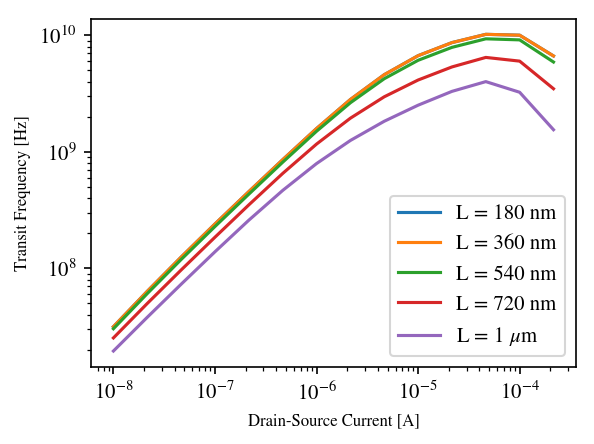
\includegraphics[width=\textwidth]{ft_nel_L}
        \resizebox {\textwidth} {!} { 
            %% Creator: Matplotlib, PGF backend
%%
%% To include the figure in your LaTeX document, write
%%   \input{<filename>.pgf}
%%
%% Make sure the required packages are loaded in your preamble
%%   \usepackage{pgf}
%%
%% Figures using additional raster images can only be included by \input if
%% they are in the same directory as the main LaTeX file. For loading figures
%% from other directories you can use the `import` package
%%   \usepackage{import}
%% and then include the figures with
%%   \import{<path to file>}{<filename>.pgf}
%%
%% Matplotlib used the following preamble
%%   \usepackage{gensymb}
%%   \usepackage[utf8x]{inputenc}
%%   \usepackage[T1]{fontenc}
%%
\begingroup%
\makeatletter%
\begin{pgfpicture}%
\pgfpathrectangle{\pgfpointorigin}{\pgfqpoint{3.840000in}{2.840000in}}%
\pgfusepath{use as bounding box, clip}%
\begin{pgfscope}%
\pgfsetbuttcap%
\pgfsetmiterjoin%
\definecolor{currentfill}{rgb}{1.000000,1.000000,1.000000}%
\pgfsetfillcolor{currentfill}%
\pgfsetlinewidth{0.000000pt}%
\definecolor{currentstroke}{rgb}{1.000000,1.000000,1.000000}%
\pgfsetstrokecolor{currentstroke}%
\pgfsetdash{}{0pt}%
\pgfpathmoveto{\pgfqpoint{0.000000in}{0.000000in}}%
\pgfpathlineto{\pgfqpoint{3.840000in}{0.000000in}}%
\pgfpathlineto{\pgfqpoint{3.840000in}{2.840000in}}%
\pgfpathlineto{\pgfqpoint{0.000000in}{2.840000in}}%
\pgfpathclose%
\pgfusepath{fill}%
\end{pgfscope}%
\begin{pgfscope}%
\pgfsetbuttcap%
\pgfsetmiterjoin%
\definecolor{currentfill}{rgb}{1.000000,1.000000,1.000000}%
\pgfsetfillcolor{currentfill}%
\pgfsetlinewidth{0.000000pt}%
\definecolor{currentstroke}{rgb}{0.000000,0.000000,0.000000}%
\pgfsetstrokecolor{currentstroke}%
\pgfsetstrokeopacity{0.000000}%
\pgfsetdash{}{0pt}%
\pgfpathmoveto{\pgfqpoint{0.761068in}{0.596026in}}%
\pgfpathlineto{\pgfqpoint{3.716667in}{0.596026in}}%
\pgfpathlineto{\pgfqpoint{3.716667in}{2.716667in}}%
\pgfpathlineto{\pgfqpoint{0.761068in}{2.716667in}}%
\pgfpathclose%
\pgfusepath{fill}%
\end{pgfscope}%
\begin{pgfscope}%
\pgfsetbuttcap%
\pgfsetroundjoin%
\definecolor{currentfill}{rgb}{0.000000,0.000000,0.000000}%
\pgfsetfillcolor{currentfill}%
\pgfsetlinewidth{0.803000pt}%
\definecolor{currentstroke}{rgb}{0.000000,0.000000,0.000000}%
\pgfsetstrokecolor{currentstroke}%
\pgfsetdash{}{0pt}%
\pgfsys@defobject{currentmarker}{\pgfqpoint{0.000000in}{-0.048611in}}{\pgfqpoint{0.000000in}{0.000000in}}{%
\pgfpathmoveto{\pgfqpoint{0.000000in}{0.000000in}}%
\pgfpathlineto{\pgfqpoint{0.000000in}{-0.048611in}}%
\pgfusepath{stroke,fill}%
}%
\begin{pgfscope}%
\pgfsys@transformshift{0.895441in}{0.596026in}%
\pgfsys@useobject{currentmarker}{}%
\end{pgfscope}%
\end{pgfscope}%
\begin{pgfscope}%
\pgftext[x=0.895441in,y=0.498804in,,top]{\fontsize{14.000000}{16.800000}\selectfont \(\displaystyle 10^{-8}\)}%
\end{pgfscope}%
\begin{pgfscope}%
\pgfsetbuttcap%
\pgfsetroundjoin%
\definecolor{currentfill}{rgb}{0.000000,0.000000,0.000000}%
\pgfsetfillcolor{currentfill}%
\pgfsetlinewidth{0.803000pt}%
\definecolor{currentstroke}{rgb}{0.000000,0.000000,0.000000}%
\pgfsetstrokecolor{currentstroke}%
\pgfsetdash{}{0pt}%
\pgfsys@defobject{currentmarker}{\pgfqpoint{0.000000in}{-0.048611in}}{\pgfqpoint{0.000000in}{0.000000in}}{%
\pgfpathmoveto{\pgfqpoint{0.000000in}{0.000000in}}%
\pgfpathlineto{\pgfqpoint{0.000000in}{-0.048611in}}%
\pgfusepath{stroke,fill}%
}%
\begin{pgfscope}%
\pgfsys@transformshift{1.515503in}{0.596026in}%
\pgfsys@useobject{currentmarker}{}%
\end{pgfscope}%
\end{pgfscope}%
\begin{pgfscope}%
\pgftext[x=1.515503in,y=0.498804in,,top]{\fontsize{14.000000}{16.800000}\selectfont \(\displaystyle 10^{-7}\)}%
\end{pgfscope}%
\begin{pgfscope}%
\pgfsetbuttcap%
\pgfsetroundjoin%
\definecolor{currentfill}{rgb}{0.000000,0.000000,0.000000}%
\pgfsetfillcolor{currentfill}%
\pgfsetlinewidth{0.803000pt}%
\definecolor{currentstroke}{rgb}{0.000000,0.000000,0.000000}%
\pgfsetstrokecolor{currentstroke}%
\pgfsetdash{}{0pt}%
\pgfsys@defobject{currentmarker}{\pgfqpoint{0.000000in}{-0.048611in}}{\pgfqpoint{0.000000in}{0.000000in}}{%
\pgfpathmoveto{\pgfqpoint{0.000000in}{0.000000in}}%
\pgfpathlineto{\pgfqpoint{0.000000in}{-0.048611in}}%
\pgfusepath{stroke,fill}%
}%
\begin{pgfscope}%
\pgfsys@transformshift{2.135564in}{0.596026in}%
\pgfsys@useobject{currentmarker}{}%
\end{pgfscope}%
\end{pgfscope}%
\begin{pgfscope}%
\pgftext[x=2.135564in,y=0.498804in,,top]{\fontsize{14.000000}{16.800000}\selectfont \(\displaystyle 10^{-6}\)}%
\end{pgfscope}%
\begin{pgfscope}%
\pgfsetbuttcap%
\pgfsetroundjoin%
\definecolor{currentfill}{rgb}{0.000000,0.000000,0.000000}%
\pgfsetfillcolor{currentfill}%
\pgfsetlinewidth{0.803000pt}%
\definecolor{currentstroke}{rgb}{0.000000,0.000000,0.000000}%
\pgfsetstrokecolor{currentstroke}%
\pgfsetdash{}{0pt}%
\pgfsys@defobject{currentmarker}{\pgfqpoint{0.000000in}{-0.048611in}}{\pgfqpoint{0.000000in}{0.000000in}}{%
\pgfpathmoveto{\pgfqpoint{0.000000in}{0.000000in}}%
\pgfpathlineto{\pgfqpoint{0.000000in}{-0.048611in}}%
\pgfusepath{stroke,fill}%
}%
\begin{pgfscope}%
\pgfsys@transformshift{2.755626in}{0.596026in}%
\pgfsys@useobject{currentmarker}{}%
\end{pgfscope}%
\end{pgfscope}%
\begin{pgfscope}%
\pgftext[x=2.755626in,y=0.498804in,,top]{\fontsize{14.000000}{16.800000}\selectfont \(\displaystyle 10^{-5}\)}%
\end{pgfscope}%
\begin{pgfscope}%
\pgfsetbuttcap%
\pgfsetroundjoin%
\definecolor{currentfill}{rgb}{0.000000,0.000000,0.000000}%
\pgfsetfillcolor{currentfill}%
\pgfsetlinewidth{0.803000pt}%
\definecolor{currentstroke}{rgb}{0.000000,0.000000,0.000000}%
\pgfsetstrokecolor{currentstroke}%
\pgfsetdash{}{0pt}%
\pgfsys@defobject{currentmarker}{\pgfqpoint{0.000000in}{-0.048611in}}{\pgfqpoint{0.000000in}{0.000000in}}{%
\pgfpathmoveto{\pgfqpoint{0.000000in}{0.000000in}}%
\pgfpathlineto{\pgfqpoint{0.000000in}{-0.048611in}}%
\pgfusepath{stroke,fill}%
}%
\begin{pgfscope}%
\pgfsys@transformshift{3.375688in}{0.596026in}%
\pgfsys@useobject{currentmarker}{}%
\end{pgfscope}%
\end{pgfscope}%
\begin{pgfscope}%
\pgftext[x=3.375688in,y=0.498804in,,top]{\fontsize{14.000000}{16.800000}\selectfont \(\displaystyle 10^{-4}\)}%
\end{pgfscope}%
\begin{pgfscope}%
\pgfsetbuttcap%
\pgfsetroundjoin%
\definecolor{currentfill}{rgb}{0.000000,0.000000,0.000000}%
\pgfsetfillcolor{currentfill}%
\pgfsetlinewidth{0.602250pt}%
\definecolor{currentstroke}{rgb}{0.000000,0.000000,0.000000}%
\pgfsetstrokecolor{currentstroke}%
\pgfsetdash{}{0pt}%
\pgfsys@defobject{currentmarker}{\pgfqpoint{0.000000in}{-0.027778in}}{\pgfqpoint{0.000000in}{0.000000in}}{%
\pgfpathmoveto{\pgfqpoint{0.000000in}{0.000000in}}%
\pgfpathlineto{\pgfqpoint{0.000000in}{-0.027778in}}%
\pgfusepath{stroke,fill}%
}%
\begin{pgfscope}%
\pgfsys@transformshift{0.757881in}{0.596026in}%
\pgfsys@useobject{currentmarker}{}%
\end{pgfscope}%
\end{pgfscope}%
\begin{pgfscope}%
\pgfsetbuttcap%
\pgfsetroundjoin%
\definecolor{currentfill}{rgb}{0.000000,0.000000,0.000000}%
\pgfsetfillcolor{currentfill}%
\pgfsetlinewidth{0.602250pt}%
\definecolor{currentstroke}{rgb}{0.000000,0.000000,0.000000}%
\pgfsetstrokecolor{currentstroke}%
\pgfsetdash{}{0pt}%
\pgfsys@defobject{currentmarker}{\pgfqpoint{0.000000in}{-0.027778in}}{\pgfqpoint{0.000000in}{0.000000in}}{%
\pgfpathmoveto{\pgfqpoint{0.000000in}{0.000000in}}%
\pgfpathlineto{\pgfqpoint{0.000000in}{-0.027778in}}%
\pgfusepath{stroke,fill}%
}%
\begin{pgfscope}%
\pgfsys@transformshift{0.799392in}{0.596026in}%
\pgfsys@useobject{currentmarker}{}%
\end{pgfscope}%
\end{pgfscope}%
\begin{pgfscope}%
\pgfsetbuttcap%
\pgfsetroundjoin%
\definecolor{currentfill}{rgb}{0.000000,0.000000,0.000000}%
\pgfsetfillcolor{currentfill}%
\pgfsetlinewidth{0.602250pt}%
\definecolor{currentstroke}{rgb}{0.000000,0.000000,0.000000}%
\pgfsetstrokecolor{currentstroke}%
\pgfsetdash{}{0pt}%
\pgfsys@defobject{currentmarker}{\pgfqpoint{0.000000in}{-0.027778in}}{\pgfqpoint{0.000000in}{0.000000in}}{%
\pgfpathmoveto{\pgfqpoint{0.000000in}{0.000000in}}%
\pgfpathlineto{\pgfqpoint{0.000000in}{-0.027778in}}%
\pgfusepath{stroke,fill}%
}%
\begin{pgfscope}%
\pgfsys@transformshift{0.835350in}{0.596026in}%
\pgfsys@useobject{currentmarker}{}%
\end{pgfscope}%
\end{pgfscope}%
\begin{pgfscope}%
\pgfsetbuttcap%
\pgfsetroundjoin%
\definecolor{currentfill}{rgb}{0.000000,0.000000,0.000000}%
\pgfsetfillcolor{currentfill}%
\pgfsetlinewidth{0.602250pt}%
\definecolor{currentstroke}{rgb}{0.000000,0.000000,0.000000}%
\pgfsetstrokecolor{currentstroke}%
\pgfsetdash{}{0pt}%
\pgfsys@defobject{currentmarker}{\pgfqpoint{0.000000in}{-0.027778in}}{\pgfqpoint{0.000000in}{0.000000in}}{%
\pgfpathmoveto{\pgfqpoint{0.000000in}{0.000000in}}%
\pgfpathlineto{\pgfqpoint{0.000000in}{-0.027778in}}%
\pgfusepath{stroke,fill}%
}%
\begin{pgfscope}%
\pgfsys@transformshift{0.867068in}{0.596026in}%
\pgfsys@useobject{currentmarker}{}%
\end{pgfscope}%
\end{pgfscope}%
\begin{pgfscope}%
\pgfsetbuttcap%
\pgfsetroundjoin%
\definecolor{currentfill}{rgb}{0.000000,0.000000,0.000000}%
\pgfsetfillcolor{currentfill}%
\pgfsetlinewidth{0.602250pt}%
\definecolor{currentstroke}{rgb}{0.000000,0.000000,0.000000}%
\pgfsetstrokecolor{currentstroke}%
\pgfsetdash{}{0pt}%
\pgfsys@defobject{currentmarker}{\pgfqpoint{0.000000in}{-0.027778in}}{\pgfqpoint{0.000000in}{0.000000in}}{%
\pgfpathmoveto{\pgfqpoint{0.000000in}{0.000000in}}%
\pgfpathlineto{\pgfqpoint{0.000000in}{-0.027778in}}%
\pgfusepath{stroke,fill}%
}%
\begin{pgfscope}%
\pgfsys@transformshift{1.082098in}{0.596026in}%
\pgfsys@useobject{currentmarker}{}%
\end{pgfscope}%
\end{pgfscope}%
\begin{pgfscope}%
\pgfsetbuttcap%
\pgfsetroundjoin%
\definecolor{currentfill}{rgb}{0.000000,0.000000,0.000000}%
\pgfsetfillcolor{currentfill}%
\pgfsetlinewidth{0.602250pt}%
\definecolor{currentstroke}{rgb}{0.000000,0.000000,0.000000}%
\pgfsetstrokecolor{currentstroke}%
\pgfsetdash{}{0pt}%
\pgfsys@defobject{currentmarker}{\pgfqpoint{0.000000in}{-0.027778in}}{\pgfqpoint{0.000000in}{0.000000in}}{%
\pgfpathmoveto{\pgfqpoint{0.000000in}{0.000000in}}%
\pgfpathlineto{\pgfqpoint{0.000000in}{-0.027778in}}%
\pgfusepath{stroke,fill}%
}%
\begin{pgfscope}%
\pgfsys@transformshift{1.191285in}{0.596026in}%
\pgfsys@useobject{currentmarker}{}%
\end{pgfscope}%
\end{pgfscope}%
\begin{pgfscope}%
\pgfsetbuttcap%
\pgfsetroundjoin%
\definecolor{currentfill}{rgb}{0.000000,0.000000,0.000000}%
\pgfsetfillcolor{currentfill}%
\pgfsetlinewidth{0.602250pt}%
\definecolor{currentstroke}{rgb}{0.000000,0.000000,0.000000}%
\pgfsetstrokecolor{currentstroke}%
\pgfsetdash{}{0pt}%
\pgfsys@defobject{currentmarker}{\pgfqpoint{0.000000in}{-0.027778in}}{\pgfqpoint{0.000000in}{0.000000in}}{%
\pgfpathmoveto{\pgfqpoint{0.000000in}{0.000000in}}%
\pgfpathlineto{\pgfqpoint{0.000000in}{-0.027778in}}%
\pgfusepath{stroke,fill}%
}%
\begin{pgfscope}%
\pgfsys@transformshift{1.268755in}{0.596026in}%
\pgfsys@useobject{currentmarker}{}%
\end{pgfscope}%
\end{pgfscope}%
\begin{pgfscope}%
\pgfsetbuttcap%
\pgfsetroundjoin%
\definecolor{currentfill}{rgb}{0.000000,0.000000,0.000000}%
\pgfsetfillcolor{currentfill}%
\pgfsetlinewidth{0.602250pt}%
\definecolor{currentstroke}{rgb}{0.000000,0.000000,0.000000}%
\pgfsetstrokecolor{currentstroke}%
\pgfsetdash{}{0pt}%
\pgfsys@defobject{currentmarker}{\pgfqpoint{0.000000in}{-0.027778in}}{\pgfqpoint{0.000000in}{0.000000in}}{%
\pgfpathmoveto{\pgfqpoint{0.000000in}{0.000000in}}%
\pgfpathlineto{\pgfqpoint{0.000000in}{-0.027778in}}%
\pgfusepath{stroke,fill}%
}%
\begin{pgfscope}%
\pgfsys@transformshift{1.328845in}{0.596026in}%
\pgfsys@useobject{currentmarker}{}%
\end{pgfscope}%
\end{pgfscope}%
\begin{pgfscope}%
\pgfsetbuttcap%
\pgfsetroundjoin%
\definecolor{currentfill}{rgb}{0.000000,0.000000,0.000000}%
\pgfsetfillcolor{currentfill}%
\pgfsetlinewidth{0.602250pt}%
\definecolor{currentstroke}{rgb}{0.000000,0.000000,0.000000}%
\pgfsetstrokecolor{currentstroke}%
\pgfsetdash{}{0pt}%
\pgfsys@defobject{currentmarker}{\pgfqpoint{0.000000in}{-0.027778in}}{\pgfqpoint{0.000000in}{0.000000in}}{%
\pgfpathmoveto{\pgfqpoint{0.000000in}{0.000000in}}%
\pgfpathlineto{\pgfqpoint{0.000000in}{-0.027778in}}%
\pgfusepath{stroke,fill}%
}%
\begin{pgfscope}%
\pgfsys@transformshift{1.377943in}{0.596026in}%
\pgfsys@useobject{currentmarker}{}%
\end{pgfscope}%
\end{pgfscope}%
\begin{pgfscope}%
\pgfsetbuttcap%
\pgfsetroundjoin%
\definecolor{currentfill}{rgb}{0.000000,0.000000,0.000000}%
\pgfsetfillcolor{currentfill}%
\pgfsetlinewidth{0.602250pt}%
\definecolor{currentstroke}{rgb}{0.000000,0.000000,0.000000}%
\pgfsetstrokecolor{currentstroke}%
\pgfsetdash{}{0pt}%
\pgfsys@defobject{currentmarker}{\pgfqpoint{0.000000in}{-0.027778in}}{\pgfqpoint{0.000000in}{0.000000in}}{%
\pgfpathmoveto{\pgfqpoint{0.000000in}{0.000000in}}%
\pgfpathlineto{\pgfqpoint{0.000000in}{-0.027778in}}%
\pgfusepath{stroke,fill}%
}%
\begin{pgfscope}%
\pgfsys@transformshift{1.419454in}{0.596026in}%
\pgfsys@useobject{currentmarker}{}%
\end{pgfscope}%
\end{pgfscope}%
\begin{pgfscope}%
\pgfsetbuttcap%
\pgfsetroundjoin%
\definecolor{currentfill}{rgb}{0.000000,0.000000,0.000000}%
\pgfsetfillcolor{currentfill}%
\pgfsetlinewidth{0.602250pt}%
\definecolor{currentstroke}{rgb}{0.000000,0.000000,0.000000}%
\pgfsetstrokecolor{currentstroke}%
\pgfsetdash{}{0pt}%
\pgfsys@defobject{currentmarker}{\pgfqpoint{0.000000in}{-0.027778in}}{\pgfqpoint{0.000000in}{0.000000in}}{%
\pgfpathmoveto{\pgfqpoint{0.000000in}{0.000000in}}%
\pgfpathlineto{\pgfqpoint{0.000000in}{-0.027778in}}%
\pgfusepath{stroke,fill}%
}%
\begin{pgfscope}%
\pgfsys@transformshift{1.455412in}{0.596026in}%
\pgfsys@useobject{currentmarker}{}%
\end{pgfscope}%
\end{pgfscope}%
\begin{pgfscope}%
\pgfsetbuttcap%
\pgfsetroundjoin%
\definecolor{currentfill}{rgb}{0.000000,0.000000,0.000000}%
\pgfsetfillcolor{currentfill}%
\pgfsetlinewidth{0.602250pt}%
\definecolor{currentstroke}{rgb}{0.000000,0.000000,0.000000}%
\pgfsetstrokecolor{currentstroke}%
\pgfsetdash{}{0pt}%
\pgfsys@defobject{currentmarker}{\pgfqpoint{0.000000in}{-0.027778in}}{\pgfqpoint{0.000000in}{0.000000in}}{%
\pgfpathmoveto{\pgfqpoint{0.000000in}{0.000000in}}%
\pgfpathlineto{\pgfqpoint{0.000000in}{-0.027778in}}%
\pgfusepath{stroke,fill}%
}%
\begin{pgfscope}%
\pgfsys@transformshift{1.487130in}{0.596026in}%
\pgfsys@useobject{currentmarker}{}%
\end{pgfscope}%
\end{pgfscope}%
\begin{pgfscope}%
\pgfsetbuttcap%
\pgfsetroundjoin%
\definecolor{currentfill}{rgb}{0.000000,0.000000,0.000000}%
\pgfsetfillcolor{currentfill}%
\pgfsetlinewidth{0.602250pt}%
\definecolor{currentstroke}{rgb}{0.000000,0.000000,0.000000}%
\pgfsetstrokecolor{currentstroke}%
\pgfsetdash{}{0pt}%
\pgfsys@defobject{currentmarker}{\pgfqpoint{0.000000in}{-0.027778in}}{\pgfqpoint{0.000000in}{0.000000in}}{%
\pgfpathmoveto{\pgfqpoint{0.000000in}{0.000000in}}%
\pgfpathlineto{\pgfqpoint{0.000000in}{-0.027778in}}%
\pgfusepath{stroke,fill}%
}%
\begin{pgfscope}%
\pgfsys@transformshift{1.702160in}{0.596026in}%
\pgfsys@useobject{currentmarker}{}%
\end{pgfscope}%
\end{pgfscope}%
\begin{pgfscope}%
\pgfsetbuttcap%
\pgfsetroundjoin%
\definecolor{currentfill}{rgb}{0.000000,0.000000,0.000000}%
\pgfsetfillcolor{currentfill}%
\pgfsetlinewidth{0.602250pt}%
\definecolor{currentstroke}{rgb}{0.000000,0.000000,0.000000}%
\pgfsetstrokecolor{currentstroke}%
\pgfsetdash{}{0pt}%
\pgfsys@defobject{currentmarker}{\pgfqpoint{0.000000in}{-0.027778in}}{\pgfqpoint{0.000000in}{0.000000in}}{%
\pgfpathmoveto{\pgfqpoint{0.000000in}{0.000000in}}%
\pgfpathlineto{\pgfqpoint{0.000000in}{-0.027778in}}%
\pgfusepath{stroke,fill}%
}%
\begin{pgfscope}%
\pgfsys@transformshift{1.811347in}{0.596026in}%
\pgfsys@useobject{currentmarker}{}%
\end{pgfscope}%
\end{pgfscope}%
\begin{pgfscope}%
\pgfsetbuttcap%
\pgfsetroundjoin%
\definecolor{currentfill}{rgb}{0.000000,0.000000,0.000000}%
\pgfsetfillcolor{currentfill}%
\pgfsetlinewidth{0.602250pt}%
\definecolor{currentstroke}{rgb}{0.000000,0.000000,0.000000}%
\pgfsetstrokecolor{currentstroke}%
\pgfsetdash{}{0pt}%
\pgfsys@defobject{currentmarker}{\pgfqpoint{0.000000in}{-0.027778in}}{\pgfqpoint{0.000000in}{0.000000in}}{%
\pgfpathmoveto{\pgfqpoint{0.000000in}{0.000000in}}%
\pgfpathlineto{\pgfqpoint{0.000000in}{-0.027778in}}%
\pgfusepath{stroke,fill}%
}%
\begin{pgfscope}%
\pgfsys@transformshift{1.888817in}{0.596026in}%
\pgfsys@useobject{currentmarker}{}%
\end{pgfscope}%
\end{pgfscope}%
\begin{pgfscope}%
\pgfsetbuttcap%
\pgfsetroundjoin%
\definecolor{currentfill}{rgb}{0.000000,0.000000,0.000000}%
\pgfsetfillcolor{currentfill}%
\pgfsetlinewidth{0.602250pt}%
\definecolor{currentstroke}{rgb}{0.000000,0.000000,0.000000}%
\pgfsetstrokecolor{currentstroke}%
\pgfsetdash{}{0pt}%
\pgfsys@defobject{currentmarker}{\pgfqpoint{0.000000in}{-0.027778in}}{\pgfqpoint{0.000000in}{0.000000in}}{%
\pgfpathmoveto{\pgfqpoint{0.000000in}{0.000000in}}%
\pgfpathlineto{\pgfqpoint{0.000000in}{-0.027778in}}%
\pgfusepath{stroke,fill}%
}%
\begin{pgfscope}%
\pgfsys@transformshift{1.948907in}{0.596026in}%
\pgfsys@useobject{currentmarker}{}%
\end{pgfscope}%
\end{pgfscope}%
\begin{pgfscope}%
\pgfsetbuttcap%
\pgfsetroundjoin%
\definecolor{currentfill}{rgb}{0.000000,0.000000,0.000000}%
\pgfsetfillcolor{currentfill}%
\pgfsetlinewidth{0.602250pt}%
\definecolor{currentstroke}{rgb}{0.000000,0.000000,0.000000}%
\pgfsetstrokecolor{currentstroke}%
\pgfsetdash{}{0pt}%
\pgfsys@defobject{currentmarker}{\pgfqpoint{0.000000in}{-0.027778in}}{\pgfqpoint{0.000000in}{0.000000in}}{%
\pgfpathmoveto{\pgfqpoint{0.000000in}{0.000000in}}%
\pgfpathlineto{\pgfqpoint{0.000000in}{-0.027778in}}%
\pgfusepath{stroke,fill}%
}%
\begin{pgfscope}%
\pgfsys@transformshift{1.998005in}{0.596026in}%
\pgfsys@useobject{currentmarker}{}%
\end{pgfscope}%
\end{pgfscope}%
\begin{pgfscope}%
\pgfsetbuttcap%
\pgfsetroundjoin%
\definecolor{currentfill}{rgb}{0.000000,0.000000,0.000000}%
\pgfsetfillcolor{currentfill}%
\pgfsetlinewidth{0.602250pt}%
\definecolor{currentstroke}{rgb}{0.000000,0.000000,0.000000}%
\pgfsetstrokecolor{currentstroke}%
\pgfsetdash{}{0pt}%
\pgfsys@defobject{currentmarker}{\pgfqpoint{0.000000in}{-0.027778in}}{\pgfqpoint{0.000000in}{0.000000in}}{%
\pgfpathmoveto{\pgfqpoint{0.000000in}{0.000000in}}%
\pgfpathlineto{\pgfqpoint{0.000000in}{-0.027778in}}%
\pgfusepath{stroke,fill}%
}%
\begin{pgfscope}%
\pgfsys@transformshift{2.039516in}{0.596026in}%
\pgfsys@useobject{currentmarker}{}%
\end{pgfscope}%
\end{pgfscope}%
\begin{pgfscope}%
\pgfsetbuttcap%
\pgfsetroundjoin%
\definecolor{currentfill}{rgb}{0.000000,0.000000,0.000000}%
\pgfsetfillcolor{currentfill}%
\pgfsetlinewidth{0.602250pt}%
\definecolor{currentstroke}{rgb}{0.000000,0.000000,0.000000}%
\pgfsetstrokecolor{currentstroke}%
\pgfsetdash{}{0pt}%
\pgfsys@defobject{currentmarker}{\pgfqpoint{0.000000in}{-0.027778in}}{\pgfqpoint{0.000000in}{0.000000in}}{%
\pgfpathmoveto{\pgfqpoint{0.000000in}{0.000000in}}%
\pgfpathlineto{\pgfqpoint{0.000000in}{-0.027778in}}%
\pgfusepath{stroke,fill}%
}%
\begin{pgfscope}%
\pgfsys@transformshift{2.075474in}{0.596026in}%
\pgfsys@useobject{currentmarker}{}%
\end{pgfscope}%
\end{pgfscope}%
\begin{pgfscope}%
\pgfsetbuttcap%
\pgfsetroundjoin%
\definecolor{currentfill}{rgb}{0.000000,0.000000,0.000000}%
\pgfsetfillcolor{currentfill}%
\pgfsetlinewidth{0.602250pt}%
\definecolor{currentstroke}{rgb}{0.000000,0.000000,0.000000}%
\pgfsetstrokecolor{currentstroke}%
\pgfsetdash{}{0pt}%
\pgfsys@defobject{currentmarker}{\pgfqpoint{0.000000in}{-0.027778in}}{\pgfqpoint{0.000000in}{0.000000in}}{%
\pgfpathmoveto{\pgfqpoint{0.000000in}{0.000000in}}%
\pgfpathlineto{\pgfqpoint{0.000000in}{-0.027778in}}%
\pgfusepath{stroke,fill}%
}%
\begin{pgfscope}%
\pgfsys@transformshift{2.107192in}{0.596026in}%
\pgfsys@useobject{currentmarker}{}%
\end{pgfscope}%
\end{pgfscope}%
\begin{pgfscope}%
\pgfsetbuttcap%
\pgfsetroundjoin%
\definecolor{currentfill}{rgb}{0.000000,0.000000,0.000000}%
\pgfsetfillcolor{currentfill}%
\pgfsetlinewidth{0.602250pt}%
\definecolor{currentstroke}{rgb}{0.000000,0.000000,0.000000}%
\pgfsetstrokecolor{currentstroke}%
\pgfsetdash{}{0pt}%
\pgfsys@defobject{currentmarker}{\pgfqpoint{0.000000in}{-0.027778in}}{\pgfqpoint{0.000000in}{0.000000in}}{%
\pgfpathmoveto{\pgfqpoint{0.000000in}{0.000000in}}%
\pgfpathlineto{\pgfqpoint{0.000000in}{-0.027778in}}%
\pgfusepath{stroke,fill}%
}%
\begin{pgfscope}%
\pgfsys@transformshift{2.322222in}{0.596026in}%
\pgfsys@useobject{currentmarker}{}%
\end{pgfscope}%
\end{pgfscope}%
\begin{pgfscope}%
\pgfsetbuttcap%
\pgfsetroundjoin%
\definecolor{currentfill}{rgb}{0.000000,0.000000,0.000000}%
\pgfsetfillcolor{currentfill}%
\pgfsetlinewidth{0.602250pt}%
\definecolor{currentstroke}{rgb}{0.000000,0.000000,0.000000}%
\pgfsetstrokecolor{currentstroke}%
\pgfsetdash{}{0pt}%
\pgfsys@defobject{currentmarker}{\pgfqpoint{0.000000in}{-0.027778in}}{\pgfqpoint{0.000000in}{0.000000in}}{%
\pgfpathmoveto{\pgfqpoint{0.000000in}{0.000000in}}%
\pgfpathlineto{\pgfqpoint{0.000000in}{-0.027778in}}%
\pgfusepath{stroke,fill}%
}%
\begin{pgfscope}%
\pgfsys@transformshift{2.431409in}{0.596026in}%
\pgfsys@useobject{currentmarker}{}%
\end{pgfscope}%
\end{pgfscope}%
\begin{pgfscope}%
\pgfsetbuttcap%
\pgfsetroundjoin%
\definecolor{currentfill}{rgb}{0.000000,0.000000,0.000000}%
\pgfsetfillcolor{currentfill}%
\pgfsetlinewidth{0.602250pt}%
\definecolor{currentstroke}{rgb}{0.000000,0.000000,0.000000}%
\pgfsetstrokecolor{currentstroke}%
\pgfsetdash{}{0pt}%
\pgfsys@defobject{currentmarker}{\pgfqpoint{0.000000in}{-0.027778in}}{\pgfqpoint{0.000000in}{0.000000in}}{%
\pgfpathmoveto{\pgfqpoint{0.000000in}{0.000000in}}%
\pgfpathlineto{\pgfqpoint{0.000000in}{-0.027778in}}%
\pgfusepath{stroke,fill}%
}%
\begin{pgfscope}%
\pgfsys@transformshift{2.508879in}{0.596026in}%
\pgfsys@useobject{currentmarker}{}%
\end{pgfscope}%
\end{pgfscope}%
\begin{pgfscope}%
\pgfsetbuttcap%
\pgfsetroundjoin%
\definecolor{currentfill}{rgb}{0.000000,0.000000,0.000000}%
\pgfsetfillcolor{currentfill}%
\pgfsetlinewidth{0.602250pt}%
\definecolor{currentstroke}{rgb}{0.000000,0.000000,0.000000}%
\pgfsetstrokecolor{currentstroke}%
\pgfsetdash{}{0pt}%
\pgfsys@defobject{currentmarker}{\pgfqpoint{0.000000in}{-0.027778in}}{\pgfqpoint{0.000000in}{0.000000in}}{%
\pgfpathmoveto{\pgfqpoint{0.000000in}{0.000000in}}%
\pgfpathlineto{\pgfqpoint{0.000000in}{-0.027778in}}%
\pgfusepath{stroke,fill}%
}%
\begin{pgfscope}%
\pgfsys@transformshift{2.568969in}{0.596026in}%
\pgfsys@useobject{currentmarker}{}%
\end{pgfscope}%
\end{pgfscope}%
\begin{pgfscope}%
\pgfsetbuttcap%
\pgfsetroundjoin%
\definecolor{currentfill}{rgb}{0.000000,0.000000,0.000000}%
\pgfsetfillcolor{currentfill}%
\pgfsetlinewidth{0.602250pt}%
\definecolor{currentstroke}{rgb}{0.000000,0.000000,0.000000}%
\pgfsetstrokecolor{currentstroke}%
\pgfsetdash{}{0pt}%
\pgfsys@defobject{currentmarker}{\pgfqpoint{0.000000in}{-0.027778in}}{\pgfqpoint{0.000000in}{0.000000in}}{%
\pgfpathmoveto{\pgfqpoint{0.000000in}{0.000000in}}%
\pgfpathlineto{\pgfqpoint{0.000000in}{-0.027778in}}%
\pgfusepath{stroke,fill}%
}%
\begin{pgfscope}%
\pgfsys@transformshift{2.618066in}{0.596026in}%
\pgfsys@useobject{currentmarker}{}%
\end{pgfscope}%
\end{pgfscope}%
\begin{pgfscope}%
\pgfsetbuttcap%
\pgfsetroundjoin%
\definecolor{currentfill}{rgb}{0.000000,0.000000,0.000000}%
\pgfsetfillcolor{currentfill}%
\pgfsetlinewidth{0.602250pt}%
\definecolor{currentstroke}{rgb}{0.000000,0.000000,0.000000}%
\pgfsetstrokecolor{currentstroke}%
\pgfsetdash{}{0pt}%
\pgfsys@defobject{currentmarker}{\pgfqpoint{0.000000in}{-0.027778in}}{\pgfqpoint{0.000000in}{0.000000in}}{%
\pgfpathmoveto{\pgfqpoint{0.000000in}{0.000000in}}%
\pgfpathlineto{\pgfqpoint{0.000000in}{-0.027778in}}%
\pgfusepath{stroke,fill}%
}%
\begin{pgfscope}%
\pgfsys@transformshift{2.659578in}{0.596026in}%
\pgfsys@useobject{currentmarker}{}%
\end{pgfscope}%
\end{pgfscope}%
\begin{pgfscope}%
\pgfsetbuttcap%
\pgfsetroundjoin%
\definecolor{currentfill}{rgb}{0.000000,0.000000,0.000000}%
\pgfsetfillcolor{currentfill}%
\pgfsetlinewidth{0.602250pt}%
\definecolor{currentstroke}{rgb}{0.000000,0.000000,0.000000}%
\pgfsetstrokecolor{currentstroke}%
\pgfsetdash{}{0pt}%
\pgfsys@defobject{currentmarker}{\pgfqpoint{0.000000in}{-0.027778in}}{\pgfqpoint{0.000000in}{0.000000in}}{%
\pgfpathmoveto{\pgfqpoint{0.000000in}{0.000000in}}%
\pgfpathlineto{\pgfqpoint{0.000000in}{-0.027778in}}%
\pgfusepath{stroke,fill}%
}%
\begin{pgfscope}%
\pgfsys@transformshift{2.695536in}{0.596026in}%
\pgfsys@useobject{currentmarker}{}%
\end{pgfscope}%
\end{pgfscope}%
\begin{pgfscope}%
\pgfsetbuttcap%
\pgfsetroundjoin%
\definecolor{currentfill}{rgb}{0.000000,0.000000,0.000000}%
\pgfsetfillcolor{currentfill}%
\pgfsetlinewidth{0.602250pt}%
\definecolor{currentstroke}{rgb}{0.000000,0.000000,0.000000}%
\pgfsetstrokecolor{currentstroke}%
\pgfsetdash{}{0pt}%
\pgfsys@defobject{currentmarker}{\pgfqpoint{0.000000in}{-0.027778in}}{\pgfqpoint{0.000000in}{0.000000in}}{%
\pgfpathmoveto{\pgfqpoint{0.000000in}{0.000000in}}%
\pgfpathlineto{\pgfqpoint{0.000000in}{-0.027778in}}%
\pgfusepath{stroke,fill}%
}%
\begin{pgfscope}%
\pgfsys@transformshift{2.727254in}{0.596026in}%
\pgfsys@useobject{currentmarker}{}%
\end{pgfscope}%
\end{pgfscope}%
\begin{pgfscope}%
\pgfsetbuttcap%
\pgfsetroundjoin%
\definecolor{currentfill}{rgb}{0.000000,0.000000,0.000000}%
\pgfsetfillcolor{currentfill}%
\pgfsetlinewidth{0.602250pt}%
\definecolor{currentstroke}{rgb}{0.000000,0.000000,0.000000}%
\pgfsetstrokecolor{currentstroke}%
\pgfsetdash{}{0pt}%
\pgfsys@defobject{currentmarker}{\pgfqpoint{0.000000in}{-0.027778in}}{\pgfqpoint{0.000000in}{0.000000in}}{%
\pgfpathmoveto{\pgfqpoint{0.000000in}{0.000000in}}%
\pgfpathlineto{\pgfqpoint{0.000000in}{-0.027778in}}%
\pgfusepath{stroke,fill}%
}%
\begin{pgfscope}%
\pgfsys@transformshift{2.942284in}{0.596026in}%
\pgfsys@useobject{currentmarker}{}%
\end{pgfscope}%
\end{pgfscope}%
\begin{pgfscope}%
\pgfsetbuttcap%
\pgfsetroundjoin%
\definecolor{currentfill}{rgb}{0.000000,0.000000,0.000000}%
\pgfsetfillcolor{currentfill}%
\pgfsetlinewidth{0.602250pt}%
\definecolor{currentstroke}{rgb}{0.000000,0.000000,0.000000}%
\pgfsetstrokecolor{currentstroke}%
\pgfsetdash{}{0pt}%
\pgfsys@defobject{currentmarker}{\pgfqpoint{0.000000in}{-0.027778in}}{\pgfqpoint{0.000000in}{0.000000in}}{%
\pgfpathmoveto{\pgfqpoint{0.000000in}{0.000000in}}%
\pgfpathlineto{\pgfqpoint{0.000000in}{-0.027778in}}%
\pgfusepath{stroke,fill}%
}%
\begin{pgfscope}%
\pgfsys@transformshift{3.051471in}{0.596026in}%
\pgfsys@useobject{currentmarker}{}%
\end{pgfscope}%
\end{pgfscope}%
\begin{pgfscope}%
\pgfsetbuttcap%
\pgfsetroundjoin%
\definecolor{currentfill}{rgb}{0.000000,0.000000,0.000000}%
\pgfsetfillcolor{currentfill}%
\pgfsetlinewidth{0.602250pt}%
\definecolor{currentstroke}{rgb}{0.000000,0.000000,0.000000}%
\pgfsetstrokecolor{currentstroke}%
\pgfsetdash{}{0pt}%
\pgfsys@defobject{currentmarker}{\pgfqpoint{0.000000in}{-0.027778in}}{\pgfqpoint{0.000000in}{0.000000in}}{%
\pgfpathmoveto{\pgfqpoint{0.000000in}{0.000000in}}%
\pgfpathlineto{\pgfqpoint{0.000000in}{-0.027778in}}%
\pgfusepath{stroke,fill}%
}%
\begin{pgfscope}%
\pgfsys@transformshift{3.128941in}{0.596026in}%
\pgfsys@useobject{currentmarker}{}%
\end{pgfscope}%
\end{pgfscope}%
\begin{pgfscope}%
\pgfsetbuttcap%
\pgfsetroundjoin%
\definecolor{currentfill}{rgb}{0.000000,0.000000,0.000000}%
\pgfsetfillcolor{currentfill}%
\pgfsetlinewidth{0.602250pt}%
\definecolor{currentstroke}{rgb}{0.000000,0.000000,0.000000}%
\pgfsetstrokecolor{currentstroke}%
\pgfsetdash{}{0pt}%
\pgfsys@defobject{currentmarker}{\pgfqpoint{0.000000in}{-0.027778in}}{\pgfqpoint{0.000000in}{0.000000in}}{%
\pgfpathmoveto{\pgfqpoint{0.000000in}{0.000000in}}%
\pgfpathlineto{\pgfqpoint{0.000000in}{-0.027778in}}%
\pgfusepath{stroke,fill}%
}%
\begin{pgfscope}%
\pgfsys@transformshift{3.189031in}{0.596026in}%
\pgfsys@useobject{currentmarker}{}%
\end{pgfscope}%
\end{pgfscope}%
\begin{pgfscope}%
\pgfsetbuttcap%
\pgfsetroundjoin%
\definecolor{currentfill}{rgb}{0.000000,0.000000,0.000000}%
\pgfsetfillcolor{currentfill}%
\pgfsetlinewidth{0.602250pt}%
\definecolor{currentstroke}{rgb}{0.000000,0.000000,0.000000}%
\pgfsetstrokecolor{currentstroke}%
\pgfsetdash{}{0pt}%
\pgfsys@defobject{currentmarker}{\pgfqpoint{0.000000in}{-0.027778in}}{\pgfqpoint{0.000000in}{0.000000in}}{%
\pgfpathmoveto{\pgfqpoint{0.000000in}{0.000000in}}%
\pgfpathlineto{\pgfqpoint{0.000000in}{-0.027778in}}%
\pgfusepath{stroke,fill}%
}%
\begin{pgfscope}%
\pgfsys@transformshift{3.238128in}{0.596026in}%
\pgfsys@useobject{currentmarker}{}%
\end{pgfscope}%
\end{pgfscope}%
\begin{pgfscope}%
\pgfsetbuttcap%
\pgfsetroundjoin%
\definecolor{currentfill}{rgb}{0.000000,0.000000,0.000000}%
\pgfsetfillcolor{currentfill}%
\pgfsetlinewidth{0.602250pt}%
\definecolor{currentstroke}{rgb}{0.000000,0.000000,0.000000}%
\pgfsetstrokecolor{currentstroke}%
\pgfsetdash{}{0pt}%
\pgfsys@defobject{currentmarker}{\pgfqpoint{0.000000in}{-0.027778in}}{\pgfqpoint{0.000000in}{0.000000in}}{%
\pgfpathmoveto{\pgfqpoint{0.000000in}{0.000000in}}%
\pgfpathlineto{\pgfqpoint{0.000000in}{-0.027778in}}%
\pgfusepath{stroke,fill}%
}%
\begin{pgfscope}%
\pgfsys@transformshift{3.279640in}{0.596026in}%
\pgfsys@useobject{currentmarker}{}%
\end{pgfscope}%
\end{pgfscope}%
\begin{pgfscope}%
\pgfsetbuttcap%
\pgfsetroundjoin%
\definecolor{currentfill}{rgb}{0.000000,0.000000,0.000000}%
\pgfsetfillcolor{currentfill}%
\pgfsetlinewidth{0.602250pt}%
\definecolor{currentstroke}{rgb}{0.000000,0.000000,0.000000}%
\pgfsetstrokecolor{currentstroke}%
\pgfsetdash{}{0pt}%
\pgfsys@defobject{currentmarker}{\pgfqpoint{0.000000in}{-0.027778in}}{\pgfqpoint{0.000000in}{0.000000in}}{%
\pgfpathmoveto{\pgfqpoint{0.000000in}{0.000000in}}%
\pgfpathlineto{\pgfqpoint{0.000000in}{-0.027778in}}%
\pgfusepath{stroke,fill}%
}%
\begin{pgfscope}%
\pgfsys@transformshift{3.315598in}{0.596026in}%
\pgfsys@useobject{currentmarker}{}%
\end{pgfscope}%
\end{pgfscope}%
\begin{pgfscope}%
\pgfsetbuttcap%
\pgfsetroundjoin%
\definecolor{currentfill}{rgb}{0.000000,0.000000,0.000000}%
\pgfsetfillcolor{currentfill}%
\pgfsetlinewidth{0.602250pt}%
\definecolor{currentstroke}{rgb}{0.000000,0.000000,0.000000}%
\pgfsetstrokecolor{currentstroke}%
\pgfsetdash{}{0pt}%
\pgfsys@defobject{currentmarker}{\pgfqpoint{0.000000in}{-0.027778in}}{\pgfqpoint{0.000000in}{0.000000in}}{%
\pgfpathmoveto{\pgfqpoint{0.000000in}{0.000000in}}%
\pgfpathlineto{\pgfqpoint{0.000000in}{-0.027778in}}%
\pgfusepath{stroke,fill}%
}%
\begin{pgfscope}%
\pgfsys@transformshift{3.347316in}{0.596026in}%
\pgfsys@useobject{currentmarker}{}%
\end{pgfscope}%
\end{pgfscope}%
\begin{pgfscope}%
\pgfsetbuttcap%
\pgfsetroundjoin%
\definecolor{currentfill}{rgb}{0.000000,0.000000,0.000000}%
\pgfsetfillcolor{currentfill}%
\pgfsetlinewidth{0.602250pt}%
\definecolor{currentstroke}{rgb}{0.000000,0.000000,0.000000}%
\pgfsetstrokecolor{currentstroke}%
\pgfsetdash{}{0pt}%
\pgfsys@defobject{currentmarker}{\pgfqpoint{0.000000in}{-0.027778in}}{\pgfqpoint{0.000000in}{0.000000in}}{%
\pgfpathmoveto{\pgfqpoint{0.000000in}{0.000000in}}%
\pgfpathlineto{\pgfqpoint{0.000000in}{-0.027778in}}%
\pgfusepath{stroke,fill}%
}%
\begin{pgfscope}%
\pgfsys@transformshift{3.562346in}{0.596026in}%
\pgfsys@useobject{currentmarker}{}%
\end{pgfscope}%
\end{pgfscope}%
\begin{pgfscope}%
\pgfsetbuttcap%
\pgfsetroundjoin%
\definecolor{currentfill}{rgb}{0.000000,0.000000,0.000000}%
\pgfsetfillcolor{currentfill}%
\pgfsetlinewidth{0.602250pt}%
\definecolor{currentstroke}{rgb}{0.000000,0.000000,0.000000}%
\pgfsetstrokecolor{currentstroke}%
\pgfsetdash{}{0pt}%
\pgfsys@defobject{currentmarker}{\pgfqpoint{0.000000in}{-0.027778in}}{\pgfqpoint{0.000000in}{0.000000in}}{%
\pgfpathmoveto{\pgfqpoint{0.000000in}{0.000000in}}%
\pgfpathlineto{\pgfqpoint{0.000000in}{-0.027778in}}%
\pgfusepath{stroke,fill}%
}%
\begin{pgfscope}%
\pgfsys@transformshift{3.671533in}{0.596026in}%
\pgfsys@useobject{currentmarker}{}%
\end{pgfscope}%
\end{pgfscope}%
\begin{pgfscope}%
\pgftext[x=2.238868in,y=0.266626in,,top]{\fontsize{12.000000}{14.400000}\selectfont Drain-Source Current [A]}%
\end{pgfscope}%
\begin{pgfscope}%
\pgfsetbuttcap%
\pgfsetroundjoin%
\definecolor{currentfill}{rgb}{0.000000,0.000000,0.000000}%
\pgfsetfillcolor{currentfill}%
\pgfsetlinewidth{0.803000pt}%
\definecolor{currentstroke}{rgb}{0.000000,0.000000,0.000000}%
\pgfsetstrokecolor{currentstroke}%
\pgfsetdash{}{0pt}%
\pgfsys@defobject{currentmarker}{\pgfqpoint{-0.048611in}{0.000000in}}{\pgfqpoint{0.000000in}{0.000000in}}{%
\pgfpathmoveto{\pgfqpoint{0.000000in}{0.000000in}}%
\pgfpathlineto{\pgfqpoint{-0.048611in}{0.000000in}}%
\pgfusepath{stroke,fill}%
}%
\begin{pgfscope}%
\pgfsys@transformshift{0.761068in}{1.195849in}%
\pgfsys@useobject{currentmarker}{}%
\end{pgfscope}%
\end{pgfscope}%
\begin{pgfscope}%
\pgftext[x=0.391626in,y=1.126983in,left,base]{\fontsize{14.000000}{16.800000}\selectfont \(\displaystyle 10^{8}\)}%
\end{pgfscope}%
\begin{pgfscope}%
\pgfsetbuttcap%
\pgfsetroundjoin%
\definecolor{currentfill}{rgb}{0.000000,0.000000,0.000000}%
\pgfsetfillcolor{currentfill}%
\pgfsetlinewidth{0.803000pt}%
\definecolor{currentstroke}{rgb}{0.000000,0.000000,0.000000}%
\pgfsetstrokecolor{currentstroke}%
\pgfsetdash{}{0pt}%
\pgfsys@defobject{currentmarker}{\pgfqpoint{-0.048611in}{0.000000in}}{\pgfqpoint{0.000000in}{0.000000in}}{%
\pgfpathmoveto{\pgfqpoint{0.000000in}{0.000000in}}%
\pgfpathlineto{\pgfqpoint{-0.048611in}{0.000000in}}%
\pgfusepath{stroke,fill}%
}%
\begin{pgfscope}%
\pgfsys@transformshift{0.761068in}{1.905162in}%
\pgfsys@useobject{currentmarker}{}%
\end{pgfscope}%
\end{pgfscope}%
\begin{pgfscope}%
\pgftext[x=0.391626in,y=1.836296in,left,base]{\fontsize{14.000000}{16.800000}\selectfont \(\displaystyle 10^{9}\)}%
\end{pgfscope}%
\begin{pgfscope}%
\pgfsetbuttcap%
\pgfsetroundjoin%
\definecolor{currentfill}{rgb}{0.000000,0.000000,0.000000}%
\pgfsetfillcolor{currentfill}%
\pgfsetlinewidth{0.803000pt}%
\definecolor{currentstroke}{rgb}{0.000000,0.000000,0.000000}%
\pgfsetstrokecolor{currentstroke}%
\pgfsetdash{}{0pt}%
\pgfsys@defobject{currentmarker}{\pgfqpoint{-0.048611in}{0.000000in}}{\pgfqpoint{0.000000in}{0.000000in}}{%
\pgfpathmoveto{\pgfqpoint{0.000000in}{0.000000in}}%
\pgfpathlineto{\pgfqpoint{-0.048611in}{0.000000in}}%
\pgfusepath{stroke,fill}%
}%
\begin{pgfscope}%
\pgfsys@transformshift{0.761068in}{2.614476in}%
\pgfsys@useobject{currentmarker}{}%
\end{pgfscope}%
\end{pgfscope}%
\begin{pgfscope}%
\pgftext[x=0.322182in,y=2.545610in,left,base]{\fontsize{14.000000}{16.800000}\selectfont \(\displaystyle 10^{10}\)}%
\end{pgfscope}%
\begin{pgfscope}%
\pgfsetbuttcap%
\pgfsetroundjoin%
\definecolor{currentfill}{rgb}{0.000000,0.000000,0.000000}%
\pgfsetfillcolor{currentfill}%
\pgfsetlinewidth{0.602250pt}%
\definecolor{currentstroke}{rgb}{0.000000,0.000000,0.000000}%
\pgfsetstrokecolor{currentstroke}%
\pgfsetdash{}{0pt}%
\pgfsys@defobject{currentmarker}{\pgfqpoint{-0.027778in}{0.000000in}}{\pgfqpoint{0.000000in}{0.000000in}}{%
\pgfpathmoveto{\pgfqpoint{0.000000in}{0.000000in}}%
\pgfpathlineto{\pgfqpoint{-0.027778in}{0.000000in}}%
\pgfusepath{stroke,fill}%
}%
\begin{pgfscope}%
\pgfsys@transformshift{0.761068in}{0.700060in}%
\pgfsys@useobject{currentmarker}{}%
\end{pgfscope}%
\end{pgfscope}%
\begin{pgfscope}%
\pgfsetbuttcap%
\pgfsetroundjoin%
\definecolor{currentfill}{rgb}{0.000000,0.000000,0.000000}%
\pgfsetfillcolor{currentfill}%
\pgfsetlinewidth{0.602250pt}%
\definecolor{currentstroke}{rgb}{0.000000,0.000000,0.000000}%
\pgfsetstrokecolor{currentstroke}%
\pgfsetdash{}{0pt}%
\pgfsys@defobject{currentmarker}{\pgfqpoint{-0.027778in}{0.000000in}}{\pgfqpoint{0.000000in}{0.000000in}}{%
\pgfpathmoveto{\pgfqpoint{0.000000in}{0.000000in}}%
\pgfpathlineto{\pgfqpoint{-0.027778in}{0.000000in}}%
\pgfusepath{stroke,fill}%
}%
\begin{pgfscope}%
\pgfsys@transformshift{0.761068in}{0.824964in}%
\pgfsys@useobject{currentmarker}{}%
\end{pgfscope}%
\end{pgfscope}%
\begin{pgfscope}%
\pgfsetbuttcap%
\pgfsetroundjoin%
\definecolor{currentfill}{rgb}{0.000000,0.000000,0.000000}%
\pgfsetfillcolor{currentfill}%
\pgfsetlinewidth{0.602250pt}%
\definecolor{currentstroke}{rgb}{0.000000,0.000000,0.000000}%
\pgfsetstrokecolor{currentstroke}%
\pgfsetdash{}{0pt}%
\pgfsys@defobject{currentmarker}{\pgfqpoint{-0.027778in}{0.000000in}}{\pgfqpoint{0.000000in}{0.000000in}}{%
\pgfpathmoveto{\pgfqpoint{0.000000in}{0.000000in}}%
\pgfpathlineto{\pgfqpoint{-0.027778in}{0.000000in}}%
\pgfusepath{stroke,fill}%
}%
\begin{pgfscope}%
\pgfsys@transformshift{0.761068in}{0.913585in}%
\pgfsys@useobject{currentmarker}{}%
\end{pgfscope}%
\end{pgfscope}%
\begin{pgfscope}%
\pgfsetbuttcap%
\pgfsetroundjoin%
\definecolor{currentfill}{rgb}{0.000000,0.000000,0.000000}%
\pgfsetfillcolor{currentfill}%
\pgfsetlinewidth{0.602250pt}%
\definecolor{currentstroke}{rgb}{0.000000,0.000000,0.000000}%
\pgfsetstrokecolor{currentstroke}%
\pgfsetdash{}{0pt}%
\pgfsys@defobject{currentmarker}{\pgfqpoint{-0.027778in}{0.000000in}}{\pgfqpoint{0.000000in}{0.000000in}}{%
\pgfpathmoveto{\pgfqpoint{0.000000in}{0.000000in}}%
\pgfpathlineto{\pgfqpoint{-0.027778in}{0.000000in}}%
\pgfusepath{stroke,fill}%
}%
\begin{pgfscope}%
\pgfsys@transformshift{0.761068in}{0.982324in}%
\pgfsys@useobject{currentmarker}{}%
\end{pgfscope}%
\end{pgfscope}%
\begin{pgfscope}%
\pgfsetbuttcap%
\pgfsetroundjoin%
\definecolor{currentfill}{rgb}{0.000000,0.000000,0.000000}%
\pgfsetfillcolor{currentfill}%
\pgfsetlinewidth{0.602250pt}%
\definecolor{currentstroke}{rgb}{0.000000,0.000000,0.000000}%
\pgfsetstrokecolor{currentstroke}%
\pgfsetdash{}{0pt}%
\pgfsys@defobject{currentmarker}{\pgfqpoint{-0.027778in}{0.000000in}}{\pgfqpoint{0.000000in}{0.000000in}}{%
\pgfpathmoveto{\pgfqpoint{0.000000in}{0.000000in}}%
\pgfpathlineto{\pgfqpoint{-0.027778in}{0.000000in}}%
\pgfusepath{stroke,fill}%
}%
\begin{pgfscope}%
\pgfsys@transformshift{0.761068in}{1.038489in}%
\pgfsys@useobject{currentmarker}{}%
\end{pgfscope}%
\end{pgfscope}%
\begin{pgfscope}%
\pgfsetbuttcap%
\pgfsetroundjoin%
\definecolor{currentfill}{rgb}{0.000000,0.000000,0.000000}%
\pgfsetfillcolor{currentfill}%
\pgfsetlinewidth{0.602250pt}%
\definecolor{currentstroke}{rgb}{0.000000,0.000000,0.000000}%
\pgfsetstrokecolor{currentstroke}%
\pgfsetdash{}{0pt}%
\pgfsys@defobject{currentmarker}{\pgfqpoint{-0.027778in}{0.000000in}}{\pgfqpoint{0.000000in}{0.000000in}}{%
\pgfpathmoveto{\pgfqpoint{0.000000in}{0.000000in}}%
\pgfpathlineto{\pgfqpoint{-0.027778in}{0.000000in}}%
\pgfusepath{stroke,fill}%
}%
\begin{pgfscope}%
\pgfsys@transformshift{0.761068in}{1.085975in}%
\pgfsys@useobject{currentmarker}{}%
\end{pgfscope}%
\end{pgfscope}%
\begin{pgfscope}%
\pgfsetbuttcap%
\pgfsetroundjoin%
\definecolor{currentfill}{rgb}{0.000000,0.000000,0.000000}%
\pgfsetfillcolor{currentfill}%
\pgfsetlinewidth{0.602250pt}%
\definecolor{currentstroke}{rgb}{0.000000,0.000000,0.000000}%
\pgfsetstrokecolor{currentstroke}%
\pgfsetdash{}{0pt}%
\pgfsys@defobject{currentmarker}{\pgfqpoint{-0.027778in}{0.000000in}}{\pgfqpoint{0.000000in}{0.000000in}}{%
\pgfpathmoveto{\pgfqpoint{0.000000in}{0.000000in}}%
\pgfpathlineto{\pgfqpoint{-0.027778in}{0.000000in}}%
\pgfusepath{stroke,fill}%
}%
\begin{pgfscope}%
\pgfsys@transformshift{0.761068in}{1.127109in}%
\pgfsys@useobject{currentmarker}{}%
\end{pgfscope}%
\end{pgfscope}%
\begin{pgfscope}%
\pgfsetbuttcap%
\pgfsetroundjoin%
\definecolor{currentfill}{rgb}{0.000000,0.000000,0.000000}%
\pgfsetfillcolor{currentfill}%
\pgfsetlinewidth{0.602250pt}%
\definecolor{currentstroke}{rgb}{0.000000,0.000000,0.000000}%
\pgfsetstrokecolor{currentstroke}%
\pgfsetdash{}{0pt}%
\pgfsys@defobject{currentmarker}{\pgfqpoint{-0.027778in}{0.000000in}}{\pgfqpoint{0.000000in}{0.000000in}}{%
\pgfpathmoveto{\pgfqpoint{0.000000in}{0.000000in}}%
\pgfpathlineto{\pgfqpoint{-0.027778in}{0.000000in}}%
\pgfusepath{stroke,fill}%
}%
\begin{pgfscope}%
\pgfsys@transformshift{0.761068in}{1.163392in}%
\pgfsys@useobject{currentmarker}{}%
\end{pgfscope}%
\end{pgfscope}%
\begin{pgfscope}%
\pgfsetbuttcap%
\pgfsetroundjoin%
\definecolor{currentfill}{rgb}{0.000000,0.000000,0.000000}%
\pgfsetfillcolor{currentfill}%
\pgfsetlinewidth{0.602250pt}%
\definecolor{currentstroke}{rgb}{0.000000,0.000000,0.000000}%
\pgfsetstrokecolor{currentstroke}%
\pgfsetdash{}{0pt}%
\pgfsys@defobject{currentmarker}{\pgfqpoint{-0.027778in}{0.000000in}}{\pgfqpoint{0.000000in}{0.000000in}}{%
\pgfpathmoveto{\pgfqpoint{0.000000in}{0.000000in}}%
\pgfpathlineto{\pgfqpoint{-0.027778in}{0.000000in}}%
\pgfusepath{stroke,fill}%
}%
\begin{pgfscope}%
\pgfsys@transformshift{0.761068in}{1.409373in}%
\pgfsys@useobject{currentmarker}{}%
\end{pgfscope}%
\end{pgfscope}%
\begin{pgfscope}%
\pgfsetbuttcap%
\pgfsetroundjoin%
\definecolor{currentfill}{rgb}{0.000000,0.000000,0.000000}%
\pgfsetfillcolor{currentfill}%
\pgfsetlinewidth{0.602250pt}%
\definecolor{currentstroke}{rgb}{0.000000,0.000000,0.000000}%
\pgfsetstrokecolor{currentstroke}%
\pgfsetdash{}{0pt}%
\pgfsys@defobject{currentmarker}{\pgfqpoint{-0.027778in}{0.000000in}}{\pgfqpoint{0.000000in}{0.000000in}}{%
\pgfpathmoveto{\pgfqpoint{0.000000in}{0.000000in}}%
\pgfpathlineto{\pgfqpoint{-0.027778in}{0.000000in}}%
\pgfusepath{stroke,fill}%
}%
\begin{pgfscope}%
\pgfsys@transformshift{0.761068in}{1.534277in}%
\pgfsys@useobject{currentmarker}{}%
\end{pgfscope}%
\end{pgfscope}%
\begin{pgfscope}%
\pgfsetbuttcap%
\pgfsetroundjoin%
\definecolor{currentfill}{rgb}{0.000000,0.000000,0.000000}%
\pgfsetfillcolor{currentfill}%
\pgfsetlinewidth{0.602250pt}%
\definecolor{currentstroke}{rgb}{0.000000,0.000000,0.000000}%
\pgfsetstrokecolor{currentstroke}%
\pgfsetdash{}{0pt}%
\pgfsys@defobject{currentmarker}{\pgfqpoint{-0.027778in}{0.000000in}}{\pgfqpoint{0.000000in}{0.000000in}}{%
\pgfpathmoveto{\pgfqpoint{0.000000in}{0.000000in}}%
\pgfpathlineto{\pgfqpoint{-0.027778in}{0.000000in}}%
\pgfusepath{stroke,fill}%
}%
\begin{pgfscope}%
\pgfsys@transformshift{0.761068in}{1.622898in}%
\pgfsys@useobject{currentmarker}{}%
\end{pgfscope}%
\end{pgfscope}%
\begin{pgfscope}%
\pgfsetbuttcap%
\pgfsetroundjoin%
\definecolor{currentfill}{rgb}{0.000000,0.000000,0.000000}%
\pgfsetfillcolor{currentfill}%
\pgfsetlinewidth{0.602250pt}%
\definecolor{currentstroke}{rgb}{0.000000,0.000000,0.000000}%
\pgfsetstrokecolor{currentstroke}%
\pgfsetdash{}{0pt}%
\pgfsys@defobject{currentmarker}{\pgfqpoint{-0.027778in}{0.000000in}}{\pgfqpoint{0.000000in}{0.000000in}}{%
\pgfpathmoveto{\pgfqpoint{0.000000in}{0.000000in}}%
\pgfpathlineto{\pgfqpoint{-0.027778in}{0.000000in}}%
\pgfusepath{stroke,fill}%
}%
\begin{pgfscope}%
\pgfsys@transformshift{0.761068in}{1.691638in}%
\pgfsys@useobject{currentmarker}{}%
\end{pgfscope}%
\end{pgfscope}%
\begin{pgfscope}%
\pgfsetbuttcap%
\pgfsetroundjoin%
\definecolor{currentfill}{rgb}{0.000000,0.000000,0.000000}%
\pgfsetfillcolor{currentfill}%
\pgfsetlinewidth{0.602250pt}%
\definecolor{currentstroke}{rgb}{0.000000,0.000000,0.000000}%
\pgfsetstrokecolor{currentstroke}%
\pgfsetdash{}{0pt}%
\pgfsys@defobject{currentmarker}{\pgfqpoint{-0.027778in}{0.000000in}}{\pgfqpoint{0.000000in}{0.000000in}}{%
\pgfpathmoveto{\pgfqpoint{0.000000in}{0.000000in}}%
\pgfpathlineto{\pgfqpoint{-0.027778in}{0.000000in}}%
\pgfusepath{stroke,fill}%
}%
\begin{pgfscope}%
\pgfsys@transformshift{0.761068in}{1.747802in}%
\pgfsys@useobject{currentmarker}{}%
\end{pgfscope}%
\end{pgfscope}%
\begin{pgfscope}%
\pgfsetbuttcap%
\pgfsetroundjoin%
\definecolor{currentfill}{rgb}{0.000000,0.000000,0.000000}%
\pgfsetfillcolor{currentfill}%
\pgfsetlinewidth{0.602250pt}%
\definecolor{currentstroke}{rgb}{0.000000,0.000000,0.000000}%
\pgfsetstrokecolor{currentstroke}%
\pgfsetdash{}{0pt}%
\pgfsys@defobject{currentmarker}{\pgfqpoint{-0.027778in}{0.000000in}}{\pgfqpoint{0.000000in}{0.000000in}}{%
\pgfpathmoveto{\pgfqpoint{0.000000in}{0.000000in}}%
\pgfpathlineto{\pgfqpoint{-0.027778in}{0.000000in}}%
\pgfusepath{stroke,fill}%
}%
\begin{pgfscope}%
\pgfsys@transformshift{0.761068in}{1.795288in}%
\pgfsys@useobject{currentmarker}{}%
\end{pgfscope}%
\end{pgfscope}%
\begin{pgfscope}%
\pgfsetbuttcap%
\pgfsetroundjoin%
\definecolor{currentfill}{rgb}{0.000000,0.000000,0.000000}%
\pgfsetfillcolor{currentfill}%
\pgfsetlinewidth{0.602250pt}%
\definecolor{currentstroke}{rgb}{0.000000,0.000000,0.000000}%
\pgfsetstrokecolor{currentstroke}%
\pgfsetdash{}{0pt}%
\pgfsys@defobject{currentmarker}{\pgfqpoint{-0.027778in}{0.000000in}}{\pgfqpoint{0.000000in}{0.000000in}}{%
\pgfpathmoveto{\pgfqpoint{0.000000in}{0.000000in}}%
\pgfpathlineto{\pgfqpoint{-0.027778in}{0.000000in}}%
\pgfusepath{stroke,fill}%
}%
\begin{pgfscope}%
\pgfsys@transformshift{0.761068in}{1.836423in}%
\pgfsys@useobject{currentmarker}{}%
\end{pgfscope}%
\end{pgfscope}%
\begin{pgfscope}%
\pgfsetbuttcap%
\pgfsetroundjoin%
\definecolor{currentfill}{rgb}{0.000000,0.000000,0.000000}%
\pgfsetfillcolor{currentfill}%
\pgfsetlinewidth{0.602250pt}%
\definecolor{currentstroke}{rgb}{0.000000,0.000000,0.000000}%
\pgfsetstrokecolor{currentstroke}%
\pgfsetdash{}{0pt}%
\pgfsys@defobject{currentmarker}{\pgfqpoint{-0.027778in}{0.000000in}}{\pgfqpoint{0.000000in}{0.000000in}}{%
\pgfpathmoveto{\pgfqpoint{0.000000in}{0.000000in}}%
\pgfpathlineto{\pgfqpoint{-0.027778in}{0.000000in}}%
\pgfusepath{stroke,fill}%
}%
\begin{pgfscope}%
\pgfsys@transformshift{0.761068in}{1.872706in}%
\pgfsys@useobject{currentmarker}{}%
\end{pgfscope}%
\end{pgfscope}%
\begin{pgfscope}%
\pgfsetbuttcap%
\pgfsetroundjoin%
\definecolor{currentfill}{rgb}{0.000000,0.000000,0.000000}%
\pgfsetfillcolor{currentfill}%
\pgfsetlinewidth{0.602250pt}%
\definecolor{currentstroke}{rgb}{0.000000,0.000000,0.000000}%
\pgfsetstrokecolor{currentstroke}%
\pgfsetdash{}{0pt}%
\pgfsys@defobject{currentmarker}{\pgfqpoint{-0.027778in}{0.000000in}}{\pgfqpoint{0.000000in}{0.000000in}}{%
\pgfpathmoveto{\pgfqpoint{0.000000in}{0.000000in}}%
\pgfpathlineto{\pgfqpoint{-0.027778in}{0.000000in}}%
\pgfusepath{stroke,fill}%
}%
\begin{pgfscope}%
\pgfsys@transformshift{0.761068in}{2.118687in}%
\pgfsys@useobject{currentmarker}{}%
\end{pgfscope}%
\end{pgfscope}%
\begin{pgfscope}%
\pgfsetbuttcap%
\pgfsetroundjoin%
\definecolor{currentfill}{rgb}{0.000000,0.000000,0.000000}%
\pgfsetfillcolor{currentfill}%
\pgfsetlinewidth{0.602250pt}%
\definecolor{currentstroke}{rgb}{0.000000,0.000000,0.000000}%
\pgfsetstrokecolor{currentstroke}%
\pgfsetdash{}{0pt}%
\pgfsys@defobject{currentmarker}{\pgfqpoint{-0.027778in}{0.000000in}}{\pgfqpoint{0.000000in}{0.000000in}}{%
\pgfpathmoveto{\pgfqpoint{0.000000in}{0.000000in}}%
\pgfpathlineto{\pgfqpoint{-0.027778in}{0.000000in}}%
\pgfusepath{stroke,fill}%
}%
\begin{pgfscope}%
\pgfsys@transformshift{0.761068in}{2.243591in}%
\pgfsys@useobject{currentmarker}{}%
\end{pgfscope}%
\end{pgfscope}%
\begin{pgfscope}%
\pgfsetbuttcap%
\pgfsetroundjoin%
\definecolor{currentfill}{rgb}{0.000000,0.000000,0.000000}%
\pgfsetfillcolor{currentfill}%
\pgfsetlinewidth{0.602250pt}%
\definecolor{currentstroke}{rgb}{0.000000,0.000000,0.000000}%
\pgfsetstrokecolor{currentstroke}%
\pgfsetdash{}{0pt}%
\pgfsys@defobject{currentmarker}{\pgfqpoint{-0.027778in}{0.000000in}}{\pgfqpoint{0.000000in}{0.000000in}}{%
\pgfpathmoveto{\pgfqpoint{0.000000in}{0.000000in}}%
\pgfpathlineto{\pgfqpoint{-0.027778in}{0.000000in}}%
\pgfusepath{stroke,fill}%
}%
\begin{pgfscope}%
\pgfsys@transformshift{0.761068in}{2.332212in}%
\pgfsys@useobject{currentmarker}{}%
\end{pgfscope}%
\end{pgfscope}%
\begin{pgfscope}%
\pgfsetbuttcap%
\pgfsetroundjoin%
\definecolor{currentfill}{rgb}{0.000000,0.000000,0.000000}%
\pgfsetfillcolor{currentfill}%
\pgfsetlinewidth{0.602250pt}%
\definecolor{currentstroke}{rgb}{0.000000,0.000000,0.000000}%
\pgfsetstrokecolor{currentstroke}%
\pgfsetdash{}{0pt}%
\pgfsys@defobject{currentmarker}{\pgfqpoint{-0.027778in}{0.000000in}}{\pgfqpoint{0.000000in}{0.000000in}}{%
\pgfpathmoveto{\pgfqpoint{0.000000in}{0.000000in}}%
\pgfpathlineto{\pgfqpoint{-0.027778in}{0.000000in}}%
\pgfusepath{stroke,fill}%
}%
\begin{pgfscope}%
\pgfsys@transformshift{0.761068in}{2.400951in}%
\pgfsys@useobject{currentmarker}{}%
\end{pgfscope}%
\end{pgfscope}%
\begin{pgfscope}%
\pgfsetbuttcap%
\pgfsetroundjoin%
\definecolor{currentfill}{rgb}{0.000000,0.000000,0.000000}%
\pgfsetfillcolor{currentfill}%
\pgfsetlinewidth{0.602250pt}%
\definecolor{currentstroke}{rgb}{0.000000,0.000000,0.000000}%
\pgfsetstrokecolor{currentstroke}%
\pgfsetdash{}{0pt}%
\pgfsys@defobject{currentmarker}{\pgfqpoint{-0.027778in}{0.000000in}}{\pgfqpoint{0.000000in}{0.000000in}}{%
\pgfpathmoveto{\pgfqpoint{0.000000in}{0.000000in}}%
\pgfpathlineto{\pgfqpoint{-0.027778in}{0.000000in}}%
\pgfusepath{stroke,fill}%
}%
\begin{pgfscope}%
\pgfsys@transformshift{0.761068in}{2.457116in}%
\pgfsys@useobject{currentmarker}{}%
\end{pgfscope}%
\end{pgfscope}%
\begin{pgfscope}%
\pgfsetbuttcap%
\pgfsetroundjoin%
\definecolor{currentfill}{rgb}{0.000000,0.000000,0.000000}%
\pgfsetfillcolor{currentfill}%
\pgfsetlinewidth{0.602250pt}%
\definecolor{currentstroke}{rgb}{0.000000,0.000000,0.000000}%
\pgfsetstrokecolor{currentstroke}%
\pgfsetdash{}{0pt}%
\pgfsys@defobject{currentmarker}{\pgfqpoint{-0.027778in}{0.000000in}}{\pgfqpoint{0.000000in}{0.000000in}}{%
\pgfpathmoveto{\pgfqpoint{0.000000in}{0.000000in}}%
\pgfpathlineto{\pgfqpoint{-0.027778in}{0.000000in}}%
\pgfusepath{stroke,fill}%
}%
\begin{pgfscope}%
\pgfsys@transformshift{0.761068in}{2.504602in}%
\pgfsys@useobject{currentmarker}{}%
\end{pgfscope}%
\end{pgfscope}%
\begin{pgfscope}%
\pgfsetbuttcap%
\pgfsetroundjoin%
\definecolor{currentfill}{rgb}{0.000000,0.000000,0.000000}%
\pgfsetfillcolor{currentfill}%
\pgfsetlinewidth{0.602250pt}%
\definecolor{currentstroke}{rgb}{0.000000,0.000000,0.000000}%
\pgfsetstrokecolor{currentstroke}%
\pgfsetdash{}{0pt}%
\pgfsys@defobject{currentmarker}{\pgfqpoint{-0.027778in}{0.000000in}}{\pgfqpoint{0.000000in}{0.000000in}}{%
\pgfpathmoveto{\pgfqpoint{0.000000in}{0.000000in}}%
\pgfpathlineto{\pgfqpoint{-0.027778in}{0.000000in}}%
\pgfusepath{stroke,fill}%
}%
\begin{pgfscope}%
\pgfsys@transformshift{0.761068in}{2.545736in}%
\pgfsys@useobject{currentmarker}{}%
\end{pgfscope}%
\end{pgfscope}%
\begin{pgfscope}%
\pgfsetbuttcap%
\pgfsetroundjoin%
\definecolor{currentfill}{rgb}{0.000000,0.000000,0.000000}%
\pgfsetfillcolor{currentfill}%
\pgfsetlinewidth{0.602250pt}%
\definecolor{currentstroke}{rgb}{0.000000,0.000000,0.000000}%
\pgfsetstrokecolor{currentstroke}%
\pgfsetdash{}{0pt}%
\pgfsys@defobject{currentmarker}{\pgfqpoint{-0.027778in}{0.000000in}}{\pgfqpoint{0.000000in}{0.000000in}}{%
\pgfpathmoveto{\pgfqpoint{0.000000in}{0.000000in}}%
\pgfpathlineto{\pgfqpoint{-0.027778in}{0.000000in}}%
\pgfusepath{stroke,fill}%
}%
\begin{pgfscope}%
\pgfsys@transformshift{0.761068in}{2.582019in}%
\pgfsys@useobject{currentmarker}{}%
\end{pgfscope}%
\end{pgfscope}%
\begin{pgfscope}%
\pgftext[x=0.266626in,y=1.656346in,,bottom,rotate=90.000000]{\fontsize{12.000000}{14.400000}\selectfont Transit Frequency [Hz]}%
\end{pgfscope}%
\begin{pgfscope}%
\pgfpathrectangle{\pgfqpoint{0.761068in}{0.596026in}}{\pgfqpoint{2.955598in}{2.120641in}} %
\pgfusepath{clip}%
\pgfsetrectcap%
\pgfsetroundjoin%
\pgfsetlinewidth{1.505625pt}%
\definecolor{currentstroke}{rgb}{0.121569,0.466667,0.705882}%
\pgfsetstrokecolor{currentstroke}%
\pgfsetdash{}{0pt}%
\pgfpathmoveto{\pgfqpoint{0.895414in}{0.840482in}}%
\pgfpathlineto{\pgfqpoint{1.102074in}{1.055808in}}%
\pgfpathlineto{\pgfqpoint{1.308781in}{1.264095in}}%
\pgfpathlineto{\pgfqpoint{1.515503in}{1.465923in}}%
\pgfpathlineto{\pgfqpoint{1.722261in}{1.662788in}}%
\pgfpathlineto{\pgfqpoint{1.928901in}{1.857085in}}%
\pgfpathlineto{\pgfqpoint{2.135564in}{2.046851in}}%
\pgfpathlineto{\pgfqpoint{2.342322in}{2.223655in}}%
\pgfpathlineto{\pgfqpoint{2.548963in}{2.374729in}}%
\pgfpathlineto{\pgfqpoint{2.755626in}{2.490418in}}%
\pgfpathlineto{\pgfqpoint{2.962259in}{2.569943in}}%
\pgfpathlineto{\pgfqpoint{3.169025in}{2.620274in}}%
\pgfpathlineto{\pgfqpoint{3.375688in}{2.615091in}}%
\pgfpathlineto{\pgfqpoint{3.582321in}{2.488708in}}%
\pgfusepath{stroke}%
\end{pgfscope}%
\begin{pgfscope}%
\pgfpathrectangle{\pgfqpoint{0.761068in}{0.596026in}}{\pgfqpoint{2.955598in}{2.120641in}} %
\pgfusepath{clip}%
\pgfsetrectcap%
\pgfsetroundjoin%
\pgfsetlinewidth{1.505625pt}%
\definecolor{currentstroke}{rgb}{1.000000,0.498039,0.054902}%
\pgfsetstrokecolor{currentstroke}%
\pgfsetdash{}{0pt}%
\pgfpathmoveto{\pgfqpoint{0.895414in}{0.840482in}}%
\pgfpathlineto{\pgfqpoint{1.102074in}{1.055808in}}%
\pgfpathlineto{\pgfqpoint{1.308781in}{1.264095in}}%
\pgfpathlineto{\pgfqpoint{1.515503in}{1.465923in}}%
\pgfpathlineto{\pgfqpoint{1.722261in}{1.662788in}}%
\pgfpathlineto{\pgfqpoint{1.928901in}{1.857085in}}%
\pgfpathlineto{\pgfqpoint{2.135564in}{2.046851in}}%
\pgfpathlineto{\pgfqpoint{2.342322in}{2.223655in}}%
\pgfpathlineto{\pgfqpoint{2.548963in}{2.374729in}}%
\pgfpathlineto{\pgfqpoint{2.755626in}{2.490418in}}%
\pgfpathlineto{\pgfqpoint{2.962259in}{2.569943in}}%
\pgfpathlineto{\pgfqpoint{3.169025in}{2.620274in}}%
\pgfpathlineto{\pgfqpoint{3.375688in}{2.615091in}}%
\pgfpathlineto{\pgfqpoint{3.582321in}{2.488708in}}%
\pgfusepath{stroke}%
\end{pgfscope}%
\begin{pgfscope}%
\pgfpathrectangle{\pgfqpoint{0.761068in}{0.596026in}}{\pgfqpoint{2.955598in}{2.120641in}} %
\pgfusepath{clip}%
\pgfsetrectcap%
\pgfsetroundjoin%
\pgfsetlinewidth{1.505625pt}%
\definecolor{currentstroke}{rgb}{0.172549,0.627451,0.172549}%
\pgfsetstrokecolor{currentstroke}%
\pgfsetdash{}{0pt}%
\pgfpathmoveto{\pgfqpoint{0.895414in}{0.828029in}}%
\pgfpathlineto{\pgfqpoint{1.102074in}{1.042163in}}%
\pgfpathlineto{\pgfqpoint{1.308781in}{1.249435in}}%
\pgfpathlineto{\pgfqpoint{1.515503in}{1.450412in}}%
\pgfpathlineto{\pgfqpoint{1.722136in}{1.647318in}}%
\pgfpathlineto{\pgfqpoint{1.928901in}{1.841729in}}%
\pgfpathlineto{\pgfqpoint{2.135564in}{2.030272in}}%
\pgfpathlineto{\pgfqpoint{2.342197in}{2.203628in}}%
\pgfpathlineto{\pgfqpoint{2.548963in}{2.350089in}}%
\pgfpathlineto{\pgfqpoint{2.755626in}{2.462157in}}%
\pgfpathlineto{\pgfqpoint{2.962384in}{2.541002in}}%
\pgfpathlineto{\pgfqpoint{3.169025in}{2.592947in}}%
\pgfpathlineto{\pgfqpoint{3.375688in}{2.586505in}}%
\pgfpathlineto{\pgfqpoint{3.582321in}{2.451677in}}%
\pgfusepath{stroke}%
\end{pgfscope}%
\begin{pgfscope}%
\pgfpathrectangle{\pgfqpoint{0.761068in}{0.596026in}}{\pgfqpoint{2.955598in}{2.120641in}} %
\pgfusepath{clip}%
\pgfsetrectcap%
\pgfsetroundjoin%
\pgfsetlinewidth{1.505625pt}%
\definecolor{currentstroke}{rgb}{0.839216,0.152941,0.156863}%
\pgfsetstrokecolor{currentstroke}%
\pgfsetdash{}{0pt}%
\pgfpathmoveto{\pgfqpoint{0.895414in}{0.772231in}}%
\pgfpathlineto{\pgfqpoint{1.102074in}{0.981893in}}%
\pgfpathlineto{\pgfqpoint{1.308781in}{1.185639in}}%
\pgfpathlineto{\pgfqpoint{1.515503in}{1.385357in}}%
\pgfpathlineto{\pgfqpoint{1.722136in}{1.582116in}}%
\pgfpathlineto{\pgfqpoint{1.928901in}{1.773406in}}%
\pgfpathlineto{\pgfqpoint{2.135564in}{1.952208in}}%
\pgfpathlineto{\pgfqpoint{2.342197in}{2.109780in}}%
\pgfpathlineto{\pgfqpoint{2.548963in}{2.240080in}}%
\pgfpathlineto{\pgfqpoint{2.755626in}{2.342139in}}%
\pgfpathlineto{\pgfqpoint{2.962384in}{2.421794in}}%
\pgfpathlineto{\pgfqpoint{3.169025in}{2.479776in}}%
\pgfpathlineto{\pgfqpoint{3.375688in}{2.457167in}}%
\pgfpathlineto{\pgfqpoint{3.582321in}{2.289135in}}%
\pgfusepath{stroke}%
\end{pgfscope}%
\begin{pgfscope}%
\pgfpathrectangle{\pgfqpoint{0.761068in}{0.596026in}}{\pgfqpoint{2.955598in}{2.120641in}} %
\pgfusepath{clip}%
\pgfsetrectcap%
\pgfsetroundjoin%
\pgfsetlinewidth{1.505625pt}%
\definecolor{currentstroke}{rgb}{0.580392,0.403922,0.741176}%
\pgfsetstrokecolor{currentstroke}%
\pgfsetdash{}{0pt}%
\pgfpathmoveto{\pgfqpoint{0.895414in}{0.692419in}}%
\pgfpathlineto{\pgfqpoint{1.102074in}{0.897865in}}%
\pgfpathlineto{\pgfqpoint{1.308781in}{1.098986in}}%
\pgfpathlineto{\pgfqpoint{1.515503in}{1.296626in}}%
\pgfpathlineto{\pgfqpoint{1.722136in}{1.488889in}}%
\pgfpathlineto{\pgfqpoint{1.928901in}{1.670010in}}%
\pgfpathlineto{\pgfqpoint{2.135564in}{1.833599in}}%
\pgfpathlineto{\pgfqpoint{2.342197in}{1.974148in}}%
\pgfpathlineto{\pgfqpoint{2.548963in}{2.091154in}}%
\pgfpathlineto{\pgfqpoint{2.755626in}{2.188902in}}%
\pgfpathlineto{\pgfqpoint{2.962259in}{2.273045in}}%
\pgfpathlineto{\pgfqpoint{3.169025in}{2.332443in}}%
\pgfpathlineto{\pgfqpoint{3.375688in}{2.267679in}}%
\pgfpathlineto{\pgfqpoint{3.582321in}{2.039570in}}%
\pgfusepath{stroke}%
\end{pgfscope}%
\begin{pgfscope}%
\pgfsetrectcap%
\pgfsetmiterjoin%
\pgfsetlinewidth{0.803000pt}%
\definecolor{currentstroke}{rgb}{0.000000,0.000000,0.000000}%
\pgfsetstrokecolor{currentstroke}%
\pgfsetdash{}{0pt}%
\pgfpathmoveto{\pgfqpoint{0.761068in}{0.596026in}}%
\pgfpathlineto{\pgfqpoint{0.761068in}{2.716667in}}%
\pgfusepath{stroke}%
\end{pgfscope}%
\begin{pgfscope}%
\pgfsetrectcap%
\pgfsetmiterjoin%
\pgfsetlinewidth{0.803000pt}%
\definecolor{currentstroke}{rgb}{0.000000,0.000000,0.000000}%
\pgfsetstrokecolor{currentstroke}%
\pgfsetdash{}{0pt}%
\pgfpathmoveto{\pgfqpoint{3.716667in}{0.596026in}}%
\pgfpathlineto{\pgfqpoint{3.716667in}{2.716667in}}%
\pgfusepath{stroke}%
\end{pgfscope}%
\begin{pgfscope}%
\pgfsetrectcap%
\pgfsetmiterjoin%
\pgfsetlinewidth{0.803000pt}%
\definecolor{currentstroke}{rgb}{0.000000,0.000000,0.000000}%
\pgfsetstrokecolor{currentstroke}%
\pgfsetdash{}{0pt}%
\pgfpathmoveto{\pgfqpoint{0.761068in}{0.596026in}}%
\pgfpathlineto{\pgfqpoint{3.716667in}{0.596026in}}%
\pgfusepath{stroke}%
\end{pgfscope}%
\begin{pgfscope}%
\pgfsetrectcap%
\pgfsetmiterjoin%
\pgfsetlinewidth{0.803000pt}%
\definecolor{currentstroke}{rgb}{0.000000,0.000000,0.000000}%
\pgfsetstrokecolor{currentstroke}%
\pgfsetdash{}{0pt}%
\pgfpathmoveto{\pgfqpoint{0.761068in}{2.716667in}}%
\pgfpathlineto{\pgfqpoint{3.716667in}{2.716667in}}%
\pgfusepath{stroke}%
\end{pgfscope}%
\begin{pgfscope}%
\pgfsetbuttcap%
\pgfsetmiterjoin%
\definecolor{currentfill}{rgb}{1.000000,1.000000,1.000000}%
\pgfsetfillcolor{currentfill}%
\pgfsetfillopacity{0.800000}%
\pgfsetlinewidth{1.003750pt}%
\definecolor{currentstroke}{rgb}{0.800000,0.800000,0.800000}%
\pgfsetstrokecolor{currentstroke}%
\pgfsetstrokeopacity{0.800000}%
\pgfsetdash{}{0pt}%
\pgfpathmoveto{\pgfqpoint{2.440226in}{0.665470in}}%
\pgfpathlineto{\pgfqpoint{3.619444in}{0.665470in}}%
\pgfpathquadraticcurveto{\pgfqpoint{3.647222in}{0.665470in}}{\pgfqpoint{3.647222in}{0.693248in}}%
\pgfpathlineto{\pgfqpoint{3.647222in}{1.647697in}}%
\pgfpathquadraticcurveto{\pgfqpoint{3.647222in}{1.675475in}}{\pgfqpoint{3.619444in}{1.675475in}}%
\pgfpathlineto{\pgfqpoint{2.440226in}{1.675475in}}%
\pgfpathquadraticcurveto{\pgfqpoint{2.412448in}{1.675475in}}{\pgfqpoint{2.412448in}{1.647697in}}%
\pgfpathlineto{\pgfqpoint{2.412448in}{0.693248in}}%
\pgfpathquadraticcurveto{\pgfqpoint{2.412448in}{0.665470in}}{\pgfqpoint{2.440226in}{0.665470in}}%
\pgfpathclose%
\pgfusepath{stroke,fill}%
\end{pgfscope}%
\begin{pgfscope}%
\pgfsetrectcap%
\pgfsetroundjoin%
\pgfsetlinewidth{1.505625pt}%
\definecolor{currentstroke}{rgb}{0.121569,0.466667,0.705882}%
\pgfsetstrokecolor{currentstroke}%
\pgfsetdash{}{0pt}%
\pgfpathmoveto{\pgfqpoint{2.468003in}{1.571308in}}%
\pgfpathlineto{\pgfqpoint{2.745781in}{1.571308in}}%
\pgfusepath{stroke}%
\end{pgfscope}%
\begin{pgfscope}%
\pgftext[x=2.856892in,y=1.522697in,left,base]{\fontsize{10.000000}{12.000000}\selectfont L = 180 nm}%
\end{pgfscope}%
\begin{pgfscope}%
\pgfsetrectcap%
\pgfsetroundjoin%
\pgfsetlinewidth{1.505625pt}%
\definecolor{currentstroke}{rgb}{1.000000,0.498039,0.054902}%
\pgfsetstrokecolor{currentstroke}%
\pgfsetdash{}{0pt}%
\pgfpathmoveto{\pgfqpoint{2.468003in}{1.377642in}}%
\pgfpathlineto{\pgfqpoint{2.745781in}{1.377642in}}%
\pgfusepath{stroke}%
\end{pgfscope}%
\begin{pgfscope}%
\pgftext[x=2.856892in,y=1.329031in,left,base]{\fontsize{10.000000}{12.000000}\selectfont L = 360 nm}%
\end{pgfscope}%
\begin{pgfscope}%
\pgfsetrectcap%
\pgfsetroundjoin%
\pgfsetlinewidth{1.505625pt}%
\definecolor{currentstroke}{rgb}{0.172549,0.627451,0.172549}%
\pgfsetstrokecolor{currentstroke}%
\pgfsetdash{}{0pt}%
\pgfpathmoveto{\pgfqpoint{2.468003in}{1.183976in}}%
\pgfpathlineto{\pgfqpoint{2.745781in}{1.183976in}}%
\pgfusepath{stroke}%
\end{pgfscope}%
\begin{pgfscope}%
\pgftext[x=2.856892in,y=1.135365in,left,base]{\fontsize{10.000000}{12.000000}\selectfont L = 540 nm}%
\end{pgfscope}%
\begin{pgfscope}%
\pgfsetrectcap%
\pgfsetroundjoin%
\pgfsetlinewidth{1.505625pt}%
\definecolor{currentstroke}{rgb}{0.839216,0.152941,0.156863}%
\pgfsetstrokecolor{currentstroke}%
\pgfsetdash{}{0pt}%
\pgfpathmoveto{\pgfqpoint{2.468003in}{0.990309in}}%
\pgfpathlineto{\pgfqpoint{2.745781in}{0.990309in}}%
\pgfusepath{stroke}%
\end{pgfscope}%
\begin{pgfscope}%
\pgftext[x=2.856892in,y=0.941698in,left,base]{\fontsize{10.000000}{12.000000}\selectfont L = 720 nm}%
\end{pgfscope}%
\begin{pgfscope}%
\pgfsetrectcap%
\pgfsetroundjoin%
\pgfsetlinewidth{1.505625pt}%
\definecolor{currentstroke}{rgb}{0.580392,0.403922,0.741176}%
\pgfsetstrokecolor{currentstroke}%
\pgfsetdash{}{0pt}%
\pgfpathmoveto{\pgfqpoint{2.468003in}{0.796643in}}%
\pgfpathlineto{\pgfqpoint{2.745781in}{0.796643in}}%
\pgfusepath{stroke}%
\end{pgfscope}%
\begin{pgfscope}%
\pgftext[x=2.856892in,y=0.748032in,left,base]{\fontsize{10.000000}{12.000000}\selectfont L = 1 \(\displaystyle \mu\)m}%
\end{pgfscope}%
\end{pgfpicture}%
\makeatother%
\endgroup%

        }
        \subcaption{L dependence at 27 \(\degree \)C}
    \end{subfigure}
    \begin{subfigure}[b]{0.48\textwidth}
        %\includegraphics[width=\textwidth]{ft_nel_T}
        \resizebox {\textwidth} {!} { 
            %% Creator: Matplotlib, PGF backend
%%
%% To include the figure in your LaTeX document, write
%%   \input{<filename>.pgf}
%%
%% Make sure the required packages are loaded in your preamble
%%   \usepackage{pgf}
%%
%% Figures using additional raster images can only be included by \input if
%% they are in the same directory as the main LaTeX file. For loading figures
%% from other directories you can use the `import` package
%%   \usepackage{import}
%% and then include the figures with
%%   \import{<path to file>}{<filename>.pgf}
%%
%% Matplotlib used the following preamble
%%   \usepackage{gensymb}
%%   \usepackage[utf8x]{inputenc}
%%   \usepackage[T1]{fontenc}
%%
\begingroup%
\makeatletter%
\begin{pgfpicture}%
\pgfpathrectangle{\pgfpointorigin}{\pgfqpoint{3.840000in}{2.840000in}}%
\pgfusepath{use as bounding box, clip}%
\begin{pgfscope}%
\pgfsetbuttcap%
\pgfsetmiterjoin%
\definecolor{currentfill}{rgb}{1.000000,1.000000,1.000000}%
\pgfsetfillcolor{currentfill}%
\pgfsetlinewidth{0.000000pt}%
\definecolor{currentstroke}{rgb}{1.000000,1.000000,1.000000}%
\pgfsetstrokecolor{currentstroke}%
\pgfsetdash{}{0pt}%
\pgfpathmoveto{\pgfqpoint{0.000000in}{0.000000in}}%
\pgfpathlineto{\pgfqpoint{3.840000in}{0.000000in}}%
\pgfpathlineto{\pgfqpoint{3.840000in}{2.840000in}}%
\pgfpathlineto{\pgfqpoint{0.000000in}{2.840000in}}%
\pgfpathclose%
\pgfusepath{fill}%
\end{pgfscope}%
\begin{pgfscope}%
\pgfsetbuttcap%
\pgfsetmiterjoin%
\definecolor{currentfill}{rgb}{1.000000,1.000000,1.000000}%
\pgfsetfillcolor{currentfill}%
\pgfsetlinewidth{0.000000pt}%
\definecolor{currentstroke}{rgb}{0.000000,0.000000,0.000000}%
\pgfsetstrokecolor{currentstroke}%
\pgfsetstrokeopacity{0.000000}%
\pgfsetdash{}{0pt}%
\pgfpathmoveto{\pgfqpoint{1.074061in}{0.596026in}}%
\pgfpathlineto{\pgfqpoint{3.716667in}{0.596026in}}%
\pgfpathlineto{\pgfqpoint{3.716667in}{2.716667in}}%
\pgfpathlineto{\pgfqpoint{1.074061in}{2.716667in}}%
\pgfpathclose%
\pgfusepath{fill}%
\end{pgfscope}%
\begin{pgfscope}%
\pgfsetbuttcap%
\pgfsetroundjoin%
\definecolor{currentfill}{rgb}{0.000000,0.000000,0.000000}%
\pgfsetfillcolor{currentfill}%
\pgfsetlinewidth{0.803000pt}%
\definecolor{currentstroke}{rgb}{0.000000,0.000000,0.000000}%
\pgfsetstrokecolor{currentstroke}%
\pgfsetdash{}{0pt}%
\pgfsys@defobject{currentmarker}{\pgfqpoint{0.000000in}{-0.048611in}}{\pgfqpoint{0.000000in}{0.000000in}}{%
\pgfpathmoveto{\pgfqpoint{0.000000in}{0.000000in}}%
\pgfpathlineto{\pgfqpoint{0.000000in}{-0.048611in}}%
\pgfusepath{stroke,fill}%
}%
\begin{pgfscope}%
\pgfsys@transformshift{1.194179in}{0.596026in}%
\pgfsys@useobject{currentmarker}{}%
\end{pgfscope}%
\end{pgfscope}%
\begin{pgfscope}%
\pgftext[x=1.194179in,y=0.498804in,,top]{\fontsize{14.000000}{16.800000}\selectfont \(\displaystyle 10^{-8}\)}%
\end{pgfscope}%
\begin{pgfscope}%
\pgfsetbuttcap%
\pgfsetroundjoin%
\definecolor{currentfill}{rgb}{0.000000,0.000000,0.000000}%
\pgfsetfillcolor{currentfill}%
\pgfsetlinewidth{0.803000pt}%
\definecolor{currentstroke}{rgb}{0.000000,0.000000,0.000000}%
\pgfsetstrokecolor{currentstroke}%
\pgfsetdash{}{0pt}%
\pgfsys@defobject{currentmarker}{\pgfqpoint{0.000000in}{-0.048611in}}{\pgfqpoint{0.000000in}{0.000000in}}{%
\pgfpathmoveto{\pgfqpoint{0.000000in}{0.000000in}}%
\pgfpathlineto{\pgfqpoint{0.000000in}{-0.048611in}}%
\pgfusepath{stroke,fill}%
}%
\begin{pgfscope}%
\pgfsys@transformshift{1.849364in}{0.596026in}%
\pgfsys@useobject{currentmarker}{}%
\end{pgfscope}%
\end{pgfscope}%
\begin{pgfscope}%
\pgftext[x=1.849364in,y=0.498804in,,top]{\fontsize{14.000000}{16.800000}\selectfont \(\displaystyle 10^{-7}\)}%
\end{pgfscope}%
\begin{pgfscope}%
\pgfsetbuttcap%
\pgfsetroundjoin%
\definecolor{currentfill}{rgb}{0.000000,0.000000,0.000000}%
\pgfsetfillcolor{currentfill}%
\pgfsetlinewidth{0.803000pt}%
\definecolor{currentstroke}{rgb}{0.000000,0.000000,0.000000}%
\pgfsetstrokecolor{currentstroke}%
\pgfsetdash{}{0pt}%
\pgfsys@defobject{currentmarker}{\pgfqpoint{0.000000in}{-0.048611in}}{\pgfqpoint{0.000000in}{0.000000in}}{%
\pgfpathmoveto{\pgfqpoint{0.000000in}{0.000000in}}%
\pgfpathlineto{\pgfqpoint{0.000000in}{-0.048611in}}%
\pgfusepath{stroke,fill}%
}%
\begin{pgfscope}%
\pgfsys@transformshift{2.504549in}{0.596026in}%
\pgfsys@useobject{currentmarker}{}%
\end{pgfscope}%
\end{pgfscope}%
\begin{pgfscope}%
\pgftext[x=2.504549in,y=0.498804in,,top]{\fontsize{14.000000}{16.800000}\selectfont \(\displaystyle 10^{-6}\)}%
\end{pgfscope}%
\begin{pgfscope}%
\pgfsetbuttcap%
\pgfsetroundjoin%
\definecolor{currentfill}{rgb}{0.000000,0.000000,0.000000}%
\pgfsetfillcolor{currentfill}%
\pgfsetlinewidth{0.803000pt}%
\definecolor{currentstroke}{rgb}{0.000000,0.000000,0.000000}%
\pgfsetstrokecolor{currentstroke}%
\pgfsetdash{}{0pt}%
\pgfsys@defobject{currentmarker}{\pgfqpoint{0.000000in}{-0.048611in}}{\pgfqpoint{0.000000in}{0.000000in}}{%
\pgfpathmoveto{\pgfqpoint{0.000000in}{0.000000in}}%
\pgfpathlineto{\pgfqpoint{0.000000in}{-0.048611in}}%
\pgfusepath{stroke,fill}%
}%
\begin{pgfscope}%
\pgfsys@transformshift{3.159733in}{0.596026in}%
\pgfsys@useobject{currentmarker}{}%
\end{pgfscope}%
\end{pgfscope}%
\begin{pgfscope}%
\pgftext[x=3.159733in,y=0.498804in,,top]{\fontsize{14.000000}{16.800000}\selectfont \(\displaystyle 10^{-5}\)}%
\end{pgfscope}%
\begin{pgfscope}%
\pgfsetbuttcap%
\pgfsetroundjoin%
\definecolor{currentfill}{rgb}{0.000000,0.000000,0.000000}%
\pgfsetfillcolor{currentfill}%
\pgfsetlinewidth{0.602250pt}%
\definecolor{currentstroke}{rgb}{0.000000,0.000000,0.000000}%
\pgfsetstrokecolor{currentstroke}%
\pgfsetdash{}{0pt}%
\pgfsys@defobject{currentmarker}{\pgfqpoint{0.000000in}{-0.027778in}}{\pgfqpoint{0.000000in}{0.000000in}}{%
\pgfpathmoveto{\pgfqpoint{0.000000in}{0.000000in}}%
\pgfpathlineto{\pgfqpoint{0.000000in}{-0.027778in}}%
\pgfusepath{stroke,fill}%
}%
\begin{pgfscope}%
\pgfsys@transformshift{1.092690in}{0.596026in}%
\pgfsys@useobject{currentmarker}{}%
\end{pgfscope}%
\end{pgfscope}%
\begin{pgfscope}%
\pgfsetbuttcap%
\pgfsetroundjoin%
\definecolor{currentfill}{rgb}{0.000000,0.000000,0.000000}%
\pgfsetfillcolor{currentfill}%
\pgfsetlinewidth{0.602250pt}%
\definecolor{currentstroke}{rgb}{0.000000,0.000000,0.000000}%
\pgfsetstrokecolor{currentstroke}%
\pgfsetdash{}{0pt}%
\pgfsys@defobject{currentmarker}{\pgfqpoint{0.000000in}{-0.027778in}}{\pgfqpoint{0.000000in}{0.000000in}}{%
\pgfpathmoveto{\pgfqpoint{0.000000in}{0.000000in}}%
\pgfpathlineto{\pgfqpoint{0.000000in}{-0.027778in}}%
\pgfusepath{stroke,fill}%
}%
\begin{pgfscope}%
\pgfsys@transformshift{1.130685in}{0.596026in}%
\pgfsys@useobject{currentmarker}{}%
\end{pgfscope}%
\end{pgfscope}%
\begin{pgfscope}%
\pgfsetbuttcap%
\pgfsetroundjoin%
\definecolor{currentfill}{rgb}{0.000000,0.000000,0.000000}%
\pgfsetfillcolor{currentfill}%
\pgfsetlinewidth{0.602250pt}%
\definecolor{currentstroke}{rgb}{0.000000,0.000000,0.000000}%
\pgfsetstrokecolor{currentstroke}%
\pgfsetdash{}{0pt}%
\pgfsys@defobject{currentmarker}{\pgfqpoint{0.000000in}{-0.027778in}}{\pgfqpoint{0.000000in}{0.000000in}}{%
\pgfpathmoveto{\pgfqpoint{0.000000in}{0.000000in}}%
\pgfpathlineto{\pgfqpoint{0.000000in}{-0.027778in}}%
\pgfusepath{stroke,fill}%
}%
\begin{pgfscope}%
\pgfsys@transformshift{1.164200in}{0.596026in}%
\pgfsys@useobject{currentmarker}{}%
\end{pgfscope}%
\end{pgfscope}%
\begin{pgfscope}%
\pgfsetbuttcap%
\pgfsetroundjoin%
\definecolor{currentfill}{rgb}{0.000000,0.000000,0.000000}%
\pgfsetfillcolor{currentfill}%
\pgfsetlinewidth{0.602250pt}%
\definecolor{currentstroke}{rgb}{0.000000,0.000000,0.000000}%
\pgfsetstrokecolor{currentstroke}%
\pgfsetdash{}{0pt}%
\pgfsys@defobject{currentmarker}{\pgfqpoint{0.000000in}{-0.027778in}}{\pgfqpoint{0.000000in}{0.000000in}}{%
\pgfpathmoveto{\pgfqpoint{0.000000in}{0.000000in}}%
\pgfpathlineto{\pgfqpoint{0.000000in}{-0.027778in}}%
\pgfusepath{stroke,fill}%
}%
\begin{pgfscope}%
\pgfsys@transformshift{1.391410in}{0.596026in}%
\pgfsys@useobject{currentmarker}{}%
\end{pgfscope}%
\end{pgfscope}%
\begin{pgfscope}%
\pgfsetbuttcap%
\pgfsetroundjoin%
\definecolor{currentfill}{rgb}{0.000000,0.000000,0.000000}%
\pgfsetfillcolor{currentfill}%
\pgfsetlinewidth{0.602250pt}%
\definecolor{currentstroke}{rgb}{0.000000,0.000000,0.000000}%
\pgfsetstrokecolor{currentstroke}%
\pgfsetdash{}{0pt}%
\pgfsys@defobject{currentmarker}{\pgfqpoint{0.000000in}{-0.027778in}}{\pgfqpoint{0.000000in}{0.000000in}}{%
\pgfpathmoveto{\pgfqpoint{0.000000in}{0.000000in}}%
\pgfpathlineto{\pgfqpoint{0.000000in}{-0.027778in}}%
\pgfusepath{stroke,fill}%
}%
\begin{pgfscope}%
\pgfsys@transformshift{1.506782in}{0.596026in}%
\pgfsys@useobject{currentmarker}{}%
\end{pgfscope}%
\end{pgfscope}%
\begin{pgfscope}%
\pgfsetbuttcap%
\pgfsetroundjoin%
\definecolor{currentfill}{rgb}{0.000000,0.000000,0.000000}%
\pgfsetfillcolor{currentfill}%
\pgfsetlinewidth{0.602250pt}%
\definecolor{currentstroke}{rgb}{0.000000,0.000000,0.000000}%
\pgfsetstrokecolor{currentstroke}%
\pgfsetdash{}{0pt}%
\pgfsys@defobject{currentmarker}{\pgfqpoint{0.000000in}{-0.027778in}}{\pgfqpoint{0.000000in}{0.000000in}}{%
\pgfpathmoveto{\pgfqpoint{0.000000in}{0.000000in}}%
\pgfpathlineto{\pgfqpoint{0.000000in}{-0.027778in}}%
\pgfusepath{stroke,fill}%
}%
\begin{pgfscope}%
\pgfsys@transformshift{1.588640in}{0.596026in}%
\pgfsys@useobject{currentmarker}{}%
\end{pgfscope}%
\end{pgfscope}%
\begin{pgfscope}%
\pgfsetbuttcap%
\pgfsetroundjoin%
\definecolor{currentfill}{rgb}{0.000000,0.000000,0.000000}%
\pgfsetfillcolor{currentfill}%
\pgfsetlinewidth{0.602250pt}%
\definecolor{currentstroke}{rgb}{0.000000,0.000000,0.000000}%
\pgfsetstrokecolor{currentstroke}%
\pgfsetdash{}{0pt}%
\pgfsys@defobject{currentmarker}{\pgfqpoint{0.000000in}{-0.027778in}}{\pgfqpoint{0.000000in}{0.000000in}}{%
\pgfpathmoveto{\pgfqpoint{0.000000in}{0.000000in}}%
\pgfpathlineto{\pgfqpoint{0.000000in}{-0.027778in}}%
\pgfusepath{stroke,fill}%
}%
\begin{pgfscope}%
\pgfsys@transformshift{1.652134in}{0.596026in}%
\pgfsys@useobject{currentmarker}{}%
\end{pgfscope}%
\end{pgfscope}%
\begin{pgfscope}%
\pgfsetbuttcap%
\pgfsetroundjoin%
\definecolor{currentfill}{rgb}{0.000000,0.000000,0.000000}%
\pgfsetfillcolor{currentfill}%
\pgfsetlinewidth{0.602250pt}%
\definecolor{currentstroke}{rgb}{0.000000,0.000000,0.000000}%
\pgfsetstrokecolor{currentstroke}%
\pgfsetdash{}{0pt}%
\pgfsys@defobject{currentmarker}{\pgfqpoint{0.000000in}{-0.027778in}}{\pgfqpoint{0.000000in}{0.000000in}}{%
\pgfpathmoveto{\pgfqpoint{0.000000in}{0.000000in}}%
\pgfpathlineto{\pgfqpoint{0.000000in}{-0.027778in}}%
\pgfusepath{stroke,fill}%
}%
\begin{pgfscope}%
\pgfsys@transformshift{1.704012in}{0.596026in}%
\pgfsys@useobject{currentmarker}{}%
\end{pgfscope}%
\end{pgfscope}%
\begin{pgfscope}%
\pgfsetbuttcap%
\pgfsetroundjoin%
\definecolor{currentfill}{rgb}{0.000000,0.000000,0.000000}%
\pgfsetfillcolor{currentfill}%
\pgfsetlinewidth{0.602250pt}%
\definecolor{currentstroke}{rgb}{0.000000,0.000000,0.000000}%
\pgfsetstrokecolor{currentstroke}%
\pgfsetdash{}{0pt}%
\pgfsys@defobject{currentmarker}{\pgfqpoint{0.000000in}{-0.027778in}}{\pgfqpoint{0.000000in}{0.000000in}}{%
\pgfpathmoveto{\pgfqpoint{0.000000in}{0.000000in}}%
\pgfpathlineto{\pgfqpoint{0.000000in}{-0.027778in}}%
\pgfusepath{stroke,fill}%
}%
\begin{pgfscope}%
\pgfsys@transformshift{1.747875in}{0.596026in}%
\pgfsys@useobject{currentmarker}{}%
\end{pgfscope}%
\end{pgfscope}%
\begin{pgfscope}%
\pgfsetbuttcap%
\pgfsetroundjoin%
\definecolor{currentfill}{rgb}{0.000000,0.000000,0.000000}%
\pgfsetfillcolor{currentfill}%
\pgfsetlinewidth{0.602250pt}%
\definecolor{currentstroke}{rgb}{0.000000,0.000000,0.000000}%
\pgfsetstrokecolor{currentstroke}%
\pgfsetdash{}{0pt}%
\pgfsys@defobject{currentmarker}{\pgfqpoint{0.000000in}{-0.027778in}}{\pgfqpoint{0.000000in}{0.000000in}}{%
\pgfpathmoveto{\pgfqpoint{0.000000in}{0.000000in}}%
\pgfpathlineto{\pgfqpoint{0.000000in}{-0.027778in}}%
\pgfusepath{stroke,fill}%
}%
\begin{pgfscope}%
\pgfsys@transformshift{1.785870in}{0.596026in}%
\pgfsys@useobject{currentmarker}{}%
\end{pgfscope}%
\end{pgfscope}%
\begin{pgfscope}%
\pgfsetbuttcap%
\pgfsetroundjoin%
\definecolor{currentfill}{rgb}{0.000000,0.000000,0.000000}%
\pgfsetfillcolor{currentfill}%
\pgfsetlinewidth{0.602250pt}%
\definecolor{currentstroke}{rgb}{0.000000,0.000000,0.000000}%
\pgfsetstrokecolor{currentstroke}%
\pgfsetdash{}{0pt}%
\pgfsys@defobject{currentmarker}{\pgfqpoint{0.000000in}{-0.027778in}}{\pgfqpoint{0.000000in}{0.000000in}}{%
\pgfpathmoveto{\pgfqpoint{0.000000in}{0.000000in}}%
\pgfpathlineto{\pgfqpoint{0.000000in}{-0.027778in}}%
\pgfusepath{stroke,fill}%
}%
\begin{pgfscope}%
\pgfsys@transformshift{1.819384in}{0.596026in}%
\pgfsys@useobject{currentmarker}{}%
\end{pgfscope}%
\end{pgfscope}%
\begin{pgfscope}%
\pgfsetbuttcap%
\pgfsetroundjoin%
\definecolor{currentfill}{rgb}{0.000000,0.000000,0.000000}%
\pgfsetfillcolor{currentfill}%
\pgfsetlinewidth{0.602250pt}%
\definecolor{currentstroke}{rgb}{0.000000,0.000000,0.000000}%
\pgfsetstrokecolor{currentstroke}%
\pgfsetdash{}{0pt}%
\pgfsys@defobject{currentmarker}{\pgfqpoint{0.000000in}{-0.027778in}}{\pgfqpoint{0.000000in}{0.000000in}}{%
\pgfpathmoveto{\pgfqpoint{0.000000in}{0.000000in}}%
\pgfpathlineto{\pgfqpoint{0.000000in}{-0.027778in}}%
\pgfusepath{stroke,fill}%
}%
\begin{pgfscope}%
\pgfsys@transformshift{2.046594in}{0.596026in}%
\pgfsys@useobject{currentmarker}{}%
\end{pgfscope}%
\end{pgfscope}%
\begin{pgfscope}%
\pgfsetbuttcap%
\pgfsetroundjoin%
\definecolor{currentfill}{rgb}{0.000000,0.000000,0.000000}%
\pgfsetfillcolor{currentfill}%
\pgfsetlinewidth{0.602250pt}%
\definecolor{currentstroke}{rgb}{0.000000,0.000000,0.000000}%
\pgfsetstrokecolor{currentstroke}%
\pgfsetdash{}{0pt}%
\pgfsys@defobject{currentmarker}{\pgfqpoint{0.000000in}{-0.027778in}}{\pgfqpoint{0.000000in}{0.000000in}}{%
\pgfpathmoveto{\pgfqpoint{0.000000in}{0.000000in}}%
\pgfpathlineto{\pgfqpoint{0.000000in}{-0.027778in}}%
\pgfusepath{stroke,fill}%
}%
\begin{pgfscope}%
\pgfsys@transformshift{2.161967in}{0.596026in}%
\pgfsys@useobject{currentmarker}{}%
\end{pgfscope}%
\end{pgfscope}%
\begin{pgfscope}%
\pgfsetbuttcap%
\pgfsetroundjoin%
\definecolor{currentfill}{rgb}{0.000000,0.000000,0.000000}%
\pgfsetfillcolor{currentfill}%
\pgfsetlinewidth{0.602250pt}%
\definecolor{currentstroke}{rgb}{0.000000,0.000000,0.000000}%
\pgfsetstrokecolor{currentstroke}%
\pgfsetdash{}{0pt}%
\pgfsys@defobject{currentmarker}{\pgfqpoint{0.000000in}{-0.027778in}}{\pgfqpoint{0.000000in}{0.000000in}}{%
\pgfpathmoveto{\pgfqpoint{0.000000in}{0.000000in}}%
\pgfpathlineto{\pgfqpoint{0.000000in}{-0.027778in}}%
\pgfusepath{stroke,fill}%
}%
\begin{pgfscope}%
\pgfsys@transformshift{2.243824in}{0.596026in}%
\pgfsys@useobject{currentmarker}{}%
\end{pgfscope}%
\end{pgfscope}%
\begin{pgfscope}%
\pgfsetbuttcap%
\pgfsetroundjoin%
\definecolor{currentfill}{rgb}{0.000000,0.000000,0.000000}%
\pgfsetfillcolor{currentfill}%
\pgfsetlinewidth{0.602250pt}%
\definecolor{currentstroke}{rgb}{0.000000,0.000000,0.000000}%
\pgfsetstrokecolor{currentstroke}%
\pgfsetdash{}{0pt}%
\pgfsys@defobject{currentmarker}{\pgfqpoint{0.000000in}{-0.027778in}}{\pgfqpoint{0.000000in}{0.000000in}}{%
\pgfpathmoveto{\pgfqpoint{0.000000in}{0.000000in}}%
\pgfpathlineto{\pgfqpoint{0.000000in}{-0.027778in}}%
\pgfusepath{stroke,fill}%
}%
\begin{pgfscope}%
\pgfsys@transformshift{2.307318in}{0.596026in}%
\pgfsys@useobject{currentmarker}{}%
\end{pgfscope}%
\end{pgfscope}%
\begin{pgfscope}%
\pgfsetbuttcap%
\pgfsetroundjoin%
\definecolor{currentfill}{rgb}{0.000000,0.000000,0.000000}%
\pgfsetfillcolor{currentfill}%
\pgfsetlinewidth{0.602250pt}%
\definecolor{currentstroke}{rgb}{0.000000,0.000000,0.000000}%
\pgfsetstrokecolor{currentstroke}%
\pgfsetdash{}{0pt}%
\pgfsys@defobject{currentmarker}{\pgfqpoint{0.000000in}{-0.027778in}}{\pgfqpoint{0.000000in}{0.000000in}}{%
\pgfpathmoveto{\pgfqpoint{0.000000in}{0.000000in}}%
\pgfpathlineto{\pgfqpoint{0.000000in}{-0.027778in}}%
\pgfusepath{stroke,fill}%
}%
\begin{pgfscope}%
\pgfsys@transformshift{2.359197in}{0.596026in}%
\pgfsys@useobject{currentmarker}{}%
\end{pgfscope}%
\end{pgfscope}%
\begin{pgfscope}%
\pgfsetbuttcap%
\pgfsetroundjoin%
\definecolor{currentfill}{rgb}{0.000000,0.000000,0.000000}%
\pgfsetfillcolor{currentfill}%
\pgfsetlinewidth{0.602250pt}%
\definecolor{currentstroke}{rgb}{0.000000,0.000000,0.000000}%
\pgfsetstrokecolor{currentstroke}%
\pgfsetdash{}{0pt}%
\pgfsys@defobject{currentmarker}{\pgfqpoint{0.000000in}{-0.027778in}}{\pgfqpoint{0.000000in}{0.000000in}}{%
\pgfpathmoveto{\pgfqpoint{0.000000in}{0.000000in}}%
\pgfpathlineto{\pgfqpoint{0.000000in}{-0.027778in}}%
\pgfusepath{stroke,fill}%
}%
\begin{pgfscope}%
\pgfsys@transformshift{2.403059in}{0.596026in}%
\pgfsys@useobject{currentmarker}{}%
\end{pgfscope}%
\end{pgfscope}%
\begin{pgfscope}%
\pgfsetbuttcap%
\pgfsetroundjoin%
\definecolor{currentfill}{rgb}{0.000000,0.000000,0.000000}%
\pgfsetfillcolor{currentfill}%
\pgfsetlinewidth{0.602250pt}%
\definecolor{currentstroke}{rgb}{0.000000,0.000000,0.000000}%
\pgfsetstrokecolor{currentstroke}%
\pgfsetdash{}{0pt}%
\pgfsys@defobject{currentmarker}{\pgfqpoint{0.000000in}{-0.027778in}}{\pgfqpoint{0.000000in}{0.000000in}}{%
\pgfpathmoveto{\pgfqpoint{0.000000in}{0.000000in}}%
\pgfpathlineto{\pgfqpoint{0.000000in}{-0.027778in}}%
\pgfusepath{stroke,fill}%
}%
\begin{pgfscope}%
\pgfsys@transformshift{2.441055in}{0.596026in}%
\pgfsys@useobject{currentmarker}{}%
\end{pgfscope}%
\end{pgfscope}%
\begin{pgfscope}%
\pgfsetbuttcap%
\pgfsetroundjoin%
\definecolor{currentfill}{rgb}{0.000000,0.000000,0.000000}%
\pgfsetfillcolor{currentfill}%
\pgfsetlinewidth{0.602250pt}%
\definecolor{currentstroke}{rgb}{0.000000,0.000000,0.000000}%
\pgfsetstrokecolor{currentstroke}%
\pgfsetdash{}{0pt}%
\pgfsys@defobject{currentmarker}{\pgfqpoint{0.000000in}{-0.027778in}}{\pgfqpoint{0.000000in}{0.000000in}}{%
\pgfpathmoveto{\pgfqpoint{0.000000in}{0.000000in}}%
\pgfpathlineto{\pgfqpoint{0.000000in}{-0.027778in}}%
\pgfusepath{stroke,fill}%
}%
\begin{pgfscope}%
\pgfsys@transformshift{2.474569in}{0.596026in}%
\pgfsys@useobject{currentmarker}{}%
\end{pgfscope}%
\end{pgfscope}%
\begin{pgfscope}%
\pgfsetbuttcap%
\pgfsetroundjoin%
\definecolor{currentfill}{rgb}{0.000000,0.000000,0.000000}%
\pgfsetfillcolor{currentfill}%
\pgfsetlinewidth{0.602250pt}%
\definecolor{currentstroke}{rgb}{0.000000,0.000000,0.000000}%
\pgfsetstrokecolor{currentstroke}%
\pgfsetdash{}{0pt}%
\pgfsys@defobject{currentmarker}{\pgfqpoint{0.000000in}{-0.027778in}}{\pgfqpoint{0.000000in}{0.000000in}}{%
\pgfpathmoveto{\pgfqpoint{0.000000in}{0.000000in}}%
\pgfpathlineto{\pgfqpoint{0.000000in}{-0.027778in}}%
\pgfusepath{stroke,fill}%
}%
\begin{pgfscope}%
\pgfsys@transformshift{2.701779in}{0.596026in}%
\pgfsys@useobject{currentmarker}{}%
\end{pgfscope}%
\end{pgfscope}%
\begin{pgfscope}%
\pgfsetbuttcap%
\pgfsetroundjoin%
\definecolor{currentfill}{rgb}{0.000000,0.000000,0.000000}%
\pgfsetfillcolor{currentfill}%
\pgfsetlinewidth{0.602250pt}%
\definecolor{currentstroke}{rgb}{0.000000,0.000000,0.000000}%
\pgfsetstrokecolor{currentstroke}%
\pgfsetdash{}{0pt}%
\pgfsys@defobject{currentmarker}{\pgfqpoint{0.000000in}{-0.027778in}}{\pgfqpoint{0.000000in}{0.000000in}}{%
\pgfpathmoveto{\pgfqpoint{0.000000in}{0.000000in}}%
\pgfpathlineto{\pgfqpoint{0.000000in}{-0.027778in}}%
\pgfusepath{stroke,fill}%
}%
\begin{pgfscope}%
\pgfsys@transformshift{2.817151in}{0.596026in}%
\pgfsys@useobject{currentmarker}{}%
\end{pgfscope}%
\end{pgfscope}%
\begin{pgfscope}%
\pgfsetbuttcap%
\pgfsetroundjoin%
\definecolor{currentfill}{rgb}{0.000000,0.000000,0.000000}%
\pgfsetfillcolor{currentfill}%
\pgfsetlinewidth{0.602250pt}%
\definecolor{currentstroke}{rgb}{0.000000,0.000000,0.000000}%
\pgfsetstrokecolor{currentstroke}%
\pgfsetdash{}{0pt}%
\pgfsys@defobject{currentmarker}{\pgfqpoint{0.000000in}{-0.027778in}}{\pgfqpoint{0.000000in}{0.000000in}}{%
\pgfpathmoveto{\pgfqpoint{0.000000in}{0.000000in}}%
\pgfpathlineto{\pgfqpoint{0.000000in}{-0.027778in}}%
\pgfusepath{stroke,fill}%
}%
\begin{pgfscope}%
\pgfsys@transformshift{2.899009in}{0.596026in}%
\pgfsys@useobject{currentmarker}{}%
\end{pgfscope}%
\end{pgfscope}%
\begin{pgfscope}%
\pgfsetbuttcap%
\pgfsetroundjoin%
\definecolor{currentfill}{rgb}{0.000000,0.000000,0.000000}%
\pgfsetfillcolor{currentfill}%
\pgfsetlinewidth{0.602250pt}%
\definecolor{currentstroke}{rgb}{0.000000,0.000000,0.000000}%
\pgfsetstrokecolor{currentstroke}%
\pgfsetdash{}{0pt}%
\pgfsys@defobject{currentmarker}{\pgfqpoint{0.000000in}{-0.027778in}}{\pgfqpoint{0.000000in}{0.000000in}}{%
\pgfpathmoveto{\pgfqpoint{0.000000in}{0.000000in}}%
\pgfpathlineto{\pgfqpoint{0.000000in}{-0.027778in}}%
\pgfusepath{stroke,fill}%
}%
\begin{pgfscope}%
\pgfsys@transformshift{2.962503in}{0.596026in}%
\pgfsys@useobject{currentmarker}{}%
\end{pgfscope}%
\end{pgfscope}%
\begin{pgfscope}%
\pgfsetbuttcap%
\pgfsetroundjoin%
\definecolor{currentfill}{rgb}{0.000000,0.000000,0.000000}%
\pgfsetfillcolor{currentfill}%
\pgfsetlinewidth{0.602250pt}%
\definecolor{currentstroke}{rgb}{0.000000,0.000000,0.000000}%
\pgfsetstrokecolor{currentstroke}%
\pgfsetdash{}{0pt}%
\pgfsys@defobject{currentmarker}{\pgfqpoint{0.000000in}{-0.027778in}}{\pgfqpoint{0.000000in}{0.000000in}}{%
\pgfpathmoveto{\pgfqpoint{0.000000in}{0.000000in}}%
\pgfpathlineto{\pgfqpoint{0.000000in}{-0.027778in}}%
\pgfusepath{stroke,fill}%
}%
\begin{pgfscope}%
\pgfsys@transformshift{3.014381in}{0.596026in}%
\pgfsys@useobject{currentmarker}{}%
\end{pgfscope}%
\end{pgfscope}%
\begin{pgfscope}%
\pgfsetbuttcap%
\pgfsetroundjoin%
\definecolor{currentfill}{rgb}{0.000000,0.000000,0.000000}%
\pgfsetfillcolor{currentfill}%
\pgfsetlinewidth{0.602250pt}%
\definecolor{currentstroke}{rgb}{0.000000,0.000000,0.000000}%
\pgfsetstrokecolor{currentstroke}%
\pgfsetdash{}{0pt}%
\pgfsys@defobject{currentmarker}{\pgfqpoint{0.000000in}{-0.027778in}}{\pgfqpoint{0.000000in}{0.000000in}}{%
\pgfpathmoveto{\pgfqpoint{0.000000in}{0.000000in}}%
\pgfpathlineto{\pgfqpoint{0.000000in}{-0.027778in}}%
\pgfusepath{stroke,fill}%
}%
\begin{pgfscope}%
\pgfsys@transformshift{3.058244in}{0.596026in}%
\pgfsys@useobject{currentmarker}{}%
\end{pgfscope}%
\end{pgfscope}%
\begin{pgfscope}%
\pgfsetbuttcap%
\pgfsetroundjoin%
\definecolor{currentfill}{rgb}{0.000000,0.000000,0.000000}%
\pgfsetfillcolor{currentfill}%
\pgfsetlinewidth{0.602250pt}%
\definecolor{currentstroke}{rgb}{0.000000,0.000000,0.000000}%
\pgfsetstrokecolor{currentstroke}%
\pgfsetdash{}{0pt}%
\pgfsys@defobject{currentmarker}{\pgfqpoint{0.000000in}{-0.027778in}}{\pgfqpoint{0.000000in}{0.000000in}}{%
\pgfpathmoveto{\pgfqpoint{0.000000in}{0.000000in}}%
\pgfpathlineto{\pgfqpoint{0.000000in}{-0.027778in}}%
\pgfusepath{stroke,fill}%
}%
\begin{pgfscope}%
\pgfsys@transformshift{3.096239in}{0.596026in}%
\pgfsys@useobject{currentmarker}{}%
\end{pgfscope}%
\end{pgfscope}%
\begin{pgfscope}%
\pgfsetbuttcap%
\pgfsetroundjoin%
\definecolor{currentfill}{rgb}{0.000000,0.000000,0.000000}%
\pgfsetfillcolor{currentfill}%
\pgfsetlinewidth{0.602250pt}%
\definecolor{currentstroke}{rgb}{0.000000,0.000000,0.000000}%
\pgfsetstrokecolor{currentstroke}%
\pgfsetdash{}{0pt}%
\pgfsys@defobject{currentmarker}{\pgfqpoint{0.000000in}{-0.027778in}}{\pgfqpoint{0.000000in}{0.000000in}}{%
\pgfpathmoveto{\pgfqpoint{0.000000in}{0.000000in}}%
\pgfpathlineto{\pgfqpoint{0.000000in}{-0.027778in}}%
\pgfusepath{stroke,fill}%
}%
\begin{pgfscope}%
\pgfsys@transformshift{3.129754in}{0.596026in}%
\pgfsys@useobject{currentmarker}{}%
\end{pgfscope}%
\end{pgfscope}%
\begin{pgfscope}%
\pgfsetbuttcap%
\pgfsetroundjoin%
\definecolor{currentfill}{rgb}{0.000000,0.000000,0.000000}%
\pgfsetfillcolor{currentfill}%
\pgfsetlinewidth{0.602250pt}%
\definecolor{currentstroke}{rgb}{0.000000,0.000000,0.000000}%
\pgfsetstrokecolor{currentstroke}%
\pgfsetdash{}{0pt}%
\pgfsys@defobject{currentmarker}{\pgfqpoint{0.000000in}{-0.027778in}}{\pgfqpoint{0.000000in}{0.000000in}}{%
\pgfpathmoveto{\pgfqpoint{0.000000in}{0.000000in}}%
\pgfpathlineto{\pgfqpoint{0.000000in}{-0.027778in}}%
\pgfusepath{stroke,fill}%
}%
\begin{pgfscope}%
\pgfsys@transformshift{3.356963in}{0.596026in}%
\pgfsys@useobject{currentmarker}{}%
\end{pgfscope}%
\end{pgfscope}%
\begin{pgfscope}%
\pgfsetbuttcap%
\pgfsetroundjoin%
\definecolor{currentfill}{rgb}{0.000000,0.000000,0.000000}%
\pgfsetfillcolor{currentfill}%
\pgfsetlinewidth{0.602250pt}%
\definecolor{currentstroke}{rgb}{0.000000,0.000000,0.000000}%
\pgfsetstrokecolor{currentstroke}%
\pgfsetdash{}{0pt}%
\pgfsys@defobject{currentmarker}{\pgfqpoint{0.000000in}{-0.027778in}}{\pgfqpoint{0.000000in}{0.000000in}}{%
\pgfpathmoveto{\pgfqpoint{0.000000in}{0.000000in}}%
\pgfpathlineto{\pgfqpoint{0.000000in}{-0.027778in}}%
\pgfusepath{stroke,fill}%
}%
\begin{pgfscope}%
\pgfsys@transformshift{3.472336in}{0.596026in}%
\pgfsys@useobject{currentmarker}{}%
\end{pgfscope}%
\end{pgfscope}%
\begin{pgfscope}%
\pgfsetbuttcap%
\pgfsetroundjoin%
\definecolor{currentfill}{rgb}{0.000000,0.000000,0.000000}%
\pgfsetfillcolor{currentfill}%
\pgfsetlinewidth{0.602250pt}%
\definecolor{currentstroke}{rgb}{0.000000,0.000000,0.000000}%
\pgfsetstrokecolor{currentstroke}%
\pgfsetdash{}{0pt}%
\pgfsys@defobject{currentmarker}{\pgfqpoint{0.000000in}{-0.027778in}}{\pgfqpoint{0.000000in}{0.000000in}}{%
\pgfpathmoveto{\pgfqpoint{0.000000in}{0.000000in}}%
\pgfpathlineto{\pgfqpoint{0.000000in}{-0.027778in}}%
\pgfusepath{stroke,fill}%
}%
\begin{pgfscope}%
\pgfsys@transformshift{3.554194in}{0.596026in}%
\pgfsys@useobject{currentmarker}{}%
\end{pgfscope}%
\end{pgfscope}%
\begin{pgfscope}%
\pgfsetbuttcap%
\pgfsetroundjoin%
\definecolor{currentfill}{rgb}{0.000000,0.000000,0.000000}%
\pgfsetfillcolor{currentfill}%
\pgfsetlinewidth{0.602250pt}%
\definecolor{currentstroke}{rgb}{0.000000,0.000000,0.000000}%
\pgfsetstrokecolor{currentstroke}%
\pgfsetdash{}{0pt}%
\pgfsys@defobject{currentmarker}{\pgfqpoint{0.000000in}{-0.027778in}}{\pgfqpoint{0.000000in}{0.000000in}}{%
\pgfpathmoveto{\pgfqpoint{0.000000in}{0.000000in}}%
\pgfpathlineto{\pgfqpoint{0.000000in}{-0.027778in}}%
\pgfusepath{stroke,fill}%
}%
\begin{pgfscope}%
\pgfsys@transformshift{3.617688in}{0.596026in}%
\pgfsys@useobject{currentmarker}{}%
\end{pgfscope}%
\end{pgfscope}%
\begin{pgfscope}%
\pgfsetbuttcap%
\pgfsetroundjoin%
\definecolor{currentfill}{rgb}{0.000000,0.000000,0.000000}%
\pgfsetfillcolor{currentfill}%
\pgfsetlinewidth{0.602250pt}%
\definecolor{currentstroke}{rgb}{0.000000,0.000000,0.000000}%
\pgfsetstrokecolor{currentstroke}%
\pgfsetdash{}{0pt}%
\pgfsys@defobject{currentmarker}{\pgfqpoint{0.000000in}{-0.027778in}}{\pgfqpoint{0.000000in}{0.000000in}}{%
\pgfpathmoveto{\pgfqpoint{0.000000in}{0.000000in}}%
\pgfpathlineto{\pgfqpoint{0.000000in}{-0.027778in}}%
\pgfusepath{stroke,fill}%
}%
\begin{pgfscope}%
\pgfsys@transformshift{3.669566in}{0.596026in}%
\pgfsys@useobject{currentmarker}{}%
\end{pgfscope}%
\end{pgfscope}%
\begin{pgfscope}%
\pgfsetbuttcap%
\pgfsetroundjoin%
\definecolor{currentfill}{rgb}{0.000000,0.000000,0.000000}%
\pgfsetfillcolor{currentfill}%
\pgfsetlinewidth{0.602250pt}%
\definecolor{currentstroke}{rgb}{0.000000,0.000000,0.000000}%
\pgfsetstrokecolor{currentstroke}%
\pgfsetdash{}{0pt}%
\pgfsys@defobject{currentmarker}{\pgfqpoint{0.000000in}{-0.027778in}}{\pgfqpoint{0.000000in}{0.000000in}}{%
\pgfpathmoveto{\pgfqpoint{0.000000in}{0.000000in}}%
\pgfpathlineto{\pgfqpoint{0.000000in}{-0.027778in}}%
\pgfusepath{stroke,fill}%
}%
\begin{pgfscope}%
\pgfsys@transformshift{3.713429in}{0.596026in}%
\pgfsys@useobject{currentmarker}{}%
\end{pgfscope}%
\end{pgfscope}%
\begin{pgfscope}%
\pgftext[x=2.395364in,y=0.266626in,,top]{\fontsize{12.000000}{14.400000}\selectfont Drain-Source Current [A]}%
\end{pgfscope}%
\begin{pgfscope}%
\pgfsetbuttcap%
\pgfsetroundjoin%
\definecolor{currentfill}{rgb}{0.000000,0.000000,0.000000}%
\pgfsetfillcolor{currentfill}%
\pgfsetlinewidth{0.803000pt}%
\definecolor{currentstroke}{rgb}{0.000000,0.000000,0.000000}%
\pgfsetstrokecolor{currentstroke}%
\pgfsetdash{}{0pt}%
\pgfsys@defobject{currentmarker}{\pgfqpoint{-0.048611in}{0.000000in}}{\pgfqpoint{0.000000in}{0.000000in}}{%
\pgfpathmoveto{\pgfqpoint{0.000000in}{0.000000in}}%
\pgfpathlineto{\pgfqpoint{-0.048611in}{0.000000in}}%
\pgfusepath{stroke,fill}%
}%
\begin{pgfscope}%
\pgfsys@transformshift{1.074061in}{0.896669in}%
\pgfsys@useobject{currentmarker}{}%
\end{pgfscope}%
\end{pgfscope}%
\begin{pgfscope}%
\pgftext[x=0.530780in,y=0.827803in,left,base]{\fontsize{14.000000}{16.800000}\selectfont \(\displaystyle 0.002\)}%
\end{pgfscope}%
\begin{pgfscope}%
\pgfsetbuttcap%
\pgfsetroundjoin%
\definecolor{currentfill}{rgb}{0.000000,0.000000,0.000000}%
\pgfsetfillcolor{currentfill}%
\pgfsetlinewidth{0.803000pt}%
\definecolor{currentstroke}{rgb}{0.000000,0.000000,0.000000}%
\pgfsetstrokecolor{currentstroke}%
\pgfsetdash{}{0pt}%
\pgfsys@defobject{currentmarker}{\pgfqpoint{-0.048611in}{0.000000in}}{\pgfqpoint{0.000000in}{0.000000in}}{%
\pgfpathmoveto{\pgfqpoint{0.000000in}{0.000000in}}%
\pgfpathlineto{\pgfqpoint{-0.048611in}{0.000000in}}%
\pgfusepath{stroke,fill}%
}%
\begin{pgfscope}%
\pgfsys@transformshift{1.074061in}{1.554583in}%
\pgfsys@useobject{currentmarker}{}%
\end{pgfscope}%
\end{pgfscope}%
\begin{pgfscope}%
\pgftext[x=0.530780in,y=1.485717in,left,base]{\fontsize{14.000000}{16.800000}\selectfont \(\displaystyle 0.004\)}%
\end{pgfscope}%
\begin{pgfscope}%
\pgfsetbuttcap%
\pgfsetroundjoin%
\definecolor{currentfill}{rgb}{0.000000,0.000000,0.000000}%
\pgfsetfillcolor{currentfill}%
\pgfsetlinewidth{0.803000pt}%
\definecolor{currentstroke}{rgb}{0.000000,0.000000,0.000000}%
\pgfsetstrokecolor{currentstroke}%
\pgfsetdash{}{0pt}%
\pgfsys@defobject{currentmarker}{\pgfqpoint{-0.048611in}{0.000000in}}{\pgfqpoint{0.000000in}{0.000000in}}{%
\pgfpathmoveto{\pgfqpoint{0.000000in}{0.000000in}}%
\pgfpathlineto{\pgfqpoint{-0.048611in}{0.000000in}}%
\pgfusepath{stroke,fill}%
}%
\begin{pgfscope}%
\pgfsys@transformshift{1.074061in}{2.212497in}%
\pgfsys@useobject{currentmarker}{}%
\end{pgfscope}%
\end{pgfscope}%
\begin{pgfscope}%
\pgftext[x=0.530780in,y=2.143631in,left,base]{\fontsize{14.000000}{16.800000}\selectfont \(\displaystyle 0.006\)}%
\end{pgfscope}%
\begin{pgfscope}%
\pgftext[x=0.475224in,y=1.656346in,,bottom,rotate=90.000000]{\fontsize{12.000000}{14.400000}\selectfont \(\displaystyle \frac{\partial f_T}{f_T \partial T}\) [Hz.Hz\(\displaystyle ^{-1}\).T\(\displaystyle ^{-1}\)]}%
\end{pgfscope}%
\begin{pgfscope}%
\pgfpathrectangle{\pgfqpoint{1.074061in}{0.596026in}}{\pgfqpoint{2.642606in}{2.120641in}} %
\pgfusepath{clip}%
\pgfsetrectcap%
\pgfsetroundjoin%
\pgfsetlinewidth{1.505625pt}%
\definecolor{currentstroke}{rgb}{0.121569,0.466667,0.705882}%
\pgfsetstrokecolor{currentstroke}%
\pgfsetdash{}{0pt}%
\pgfpathmoveto{\pgfqpoint{1.194179in}{0.872749in}}%
\pgfpathlineto{\pgfqpoint{1.412517in}{0.781890in}}%
\pgfpathlineto{\pgfqpoint{1.630994in}{0.715786in}}%
\pgfpathlineto{\pgfqpoint{1.849364in}{0.692419in}}%
\pgfpathlineto{\pgfqpoint{2.067701in}{0.711903in}}%
\pgfpathlineto{\pgfqpoint{2.286179in}{0.758948in}}%
\pgfpathlineto{\pgfqpoint{2.504549in}{0.811838in}}%
\pgfpathlineto{\pgfqpoint{2.722886in}{0.853643in}}%
\pgfpathlineto{\pgfqpoint{2.941364in}{0.883407in}}%
\pgfpathlineto{\pgfqpoint{3.159733in}{0.964459in}}%
\pgfpathlineto{\pgfqpoint{3.378071in}{1.325468in}}%
\pgfpathlineto{\pgfqpoint{3.596548in}{1.807753in}}%
\pgfusepath{stroke}%
\end{pgfscope}%
\begin{pgfscope}%
\pgfpathrectangle{\pgfqpoint{1.074061in}{0.596026in}}{\pgfqpoint{2.642606in}{2.120641in}} %
\pgfusepath{clip}%
\pgfsetrectcap%
\pgfsetroundjoin%
\pgfsetlinewidth{1.505625pt}%
\definecolor{currentstroke}{rgb}{1.000000,0.498039,0.054902}%
\pgfsetstrokecolor{currentstroke}%
\pgfsetdash{}{0pt}%
\pgfpathmoveto{\pgfqpoint{1.194179in}{0.872749in}}%
\pgfpathlineto{\pgfqpoint{1.412517in}{0.781890in}}%
\pgfpathlineto{\pgfqpoint{1.630994in}{0.715786in}}%
\pgfpathlineto{\pgfqpoint{1.849364in}{0.692419in}}%
\pgfpathlineto{\pgfqpoint{2.067701in}{0.711903in}}%
\pgfpathlineto{\pgfqpoint{2.286179in}{0.758948in}}%
\pgfpathlineto{\pgfqpoint{2.504549in}{0.811838in}}%
\pgfpathlineto{\pgfqpoint{2.722886in}{0.853643in}}%
\pgfpathlineto{\pgfqpoint{2.941364in}{0.883407in}}%
\pgfpathlineto{\pgfqpoint{3.159733in}{0.964459in}}%
\pgfpathlineto{\pgfqpoint{3.378071in}{1.325468in}}%
\pgfpathlineto{\pgfqpoint{3.596548in}{1.807753in}}%
\pgfusepath{stroke}%
\end{pgfscope}%
\begin{pgfscope}%
\pgfpathrectangle{\pgfqpoint{1.074061in}{0.596026in}}{\pgfqpoint{2.642606in}{2.120641in}} %
\pgfusepath{clip}%
\pgfsetrectcap%
\pgfsetroundjoin%
\pgfsetlinewidth{1.505625pt}%
\definecolor{currentstroke}{rgb}{0.172549,0.627451,0.172549}%
\pgfsetstrokecolor{currentstroke}%
\pgfsetdash{}{0pt}%
\pgfpathmoveto{\pgfqpoint{1.194179in}{0.876672in}}%
\pgfpathlineto{\pgfqpoint{1.412517in}{0.788149in}}%
\pgfpathlineto{\pgfqpoint{1.630994in}{0.726242in}}%
\pgfpathlineto{\pgfqpoint{1.849364in}{0.705341in}}%
\pgfpathlineto{\pgfqpoint{2.067701in}{0.727026in}}%
\pgfpathlineto{\pgfqpoint{2.286179in}{0.774826in}}%
\pgfpathlineto{\pgfqpoint{2.504549in}{0.827863in}}%
\pgfpathlineto{\pgfqpoint{2.722886in}{0.871238in}}%
\pgfpathlineto{\pgfqpoint{2.941364in}{0.910518in}}%
\pgfpathlineto{\pgfqpoint{3.159733in}{1.021700in}}%
\pgfpathlineto{\pgfqpoint{3.378071in}{1.436496in}}%
\pgfpathlineto{\pgfqpoint{3.596548in}{1.929324in}}%
\pgfusepath{stroke}%
\end{pgfscope}%
\begin{pgfscope}%
\pgfpathrectangle{\pgfqpoint{1.074061in}{0.596026in}}{\pgfqpoint{2.642606in}{2.120641in}} %
\pgfusepath{clip}%
\pgfsetrectcap%
\pgfsetroundjoin%
\pgfsetlinewidth{1.505625pt}%
\definecolor{currentstroke}{rgb}{0.839216,0.152941,0.156863}%
\pgfsetstrokecolor{currentstroke}%
\pgfsetdash{}{0pt}%
\pgfpathmoveto{\pgfqpoint{1.194179in}{0.882121in}}%
\pgfpathlineto{\pgfqpoint{1.412517in}{0.803298in}}%
\pgfpathlineto{\pgfqpoint{1.630994in}{0.755700in}}%
\pgfpathlineto{\pgfqpoint{1.849364in}{0.747481in}}%
\pgfpathlineto{\pgfqpoint{2.067701in}{0.774881in}}%
\pgfpathlineto{\pgfqpoint{2.286179in}{0.821437in}}%
\pgfpathlineto{\pgfqpoint{2.504549in}{0.873002in}}%
\pgfpathlineto{\pgfqpoint{2.722886in}{0.926759in}}%
\pgfpathlineto{\pgfqpoint{2.941364in}{1.007744in}}%
\pgfpathlineto{\pgfqpoint{3.159733in}{1.244438in}}%
\pgfpathlineto{\pgfqpoint{3.378071in}{1.817137in}}%
\pgfpathlineto{\pgfqpoint{3.596548in}{2.305100in}}%
\pgfusepath{stroke}%
\end{pgfscope}%
\begin{pgfscope}%
\pgfpathrectangle{\pgfqpoint{1.074061in}{0.596026in}}{\pgfqpoint{2.642606in}{2.120641in}} %
\pgfusepath{clip}%
\pgfsetrectcap%
\pgfsetroundjoin%
\pgfsetlinewidth{1.505625pt}%
\definecolor{currentstroke}{rgb}{0.580392,0.403922,0.741176}%
\pgfsetstrokecolor{currentstroke}%
\pgfsetdash{}{0pt}%
\pgfpathmoveto{\pgfqpoint{1.194179in}{0.879937in}}%
\pgfpathlineto{\pgfqpoint{1.412517in}{0.812547in}}%
\pgfpathlineto{\pgfqpoint{1.630994in}{0.778014in}}%
\pgfpathlineto{\pgfqpoint{1.849364in}{0.780183in}}%
\pgfpathlineto{\pgfqpoint{2.067701in}{0.810012in}}%
\pgfpathlineto{\pgfqpoint{2.286179in}{0.854210in}}%
\pgfpathlineto{\pgfqpoint{2.504549in}{0.907607in}}%
\pgfpathlineto{\pgfqpoint{2.722886in}{0.979172in}}%
\pgfpathlineto{\pgfqpoint{2.941364in}{1.124062in}}%
\pgfpathlineto{\pgfqpoint{3.159733in}{1.532363in}}%
\pgfpathlineto{\pgfqpoint{3.378071in}{2.165967in}}%
\pgfpathlineto{\pgfqpoint{3.596548in}{2.620274in}}%
\pgfusepath{stroke}%
\end{pgfscope}%
\begin{pgfscope}%
\pgfsetrectcap%
\pgfsetmiterjoin%
\pgfsetlinewidth{0.803000pt}%
\definecolor{currentstroke}{rgb}{0.000000,0.000000,0.000000}%
\pgfsetstrokecolor{currentstroke}%
\pgfsetdash{}{0pt}%
\pgfpathmoveto{\pgfqpoint{1.074061in}{0.596026in}}%
\pgfpathlineto{\pgfqpoint{1.074061in}{2.716667in}}%
\pgfusepath{stroke}%
\end{pgfscope}%
\begin{pgfscope}%
\pgfsetrectcap%
\pgfsetmiterjoin%
\pgfsetlinewidth{0.803000pt}%
\definecolor{currentstroke}{rgb}{0.000000,0.000000,0.000000}%
\pgfsetstrokecolor{currentstroke}%
\pgfsetdash{}{0pt}%
\pgfpathmoveto{\pgfqpoint{3.716667in}{0.596026in}}%
\pgfpathlineto{\pgfqpoint{3.716667in}{2.716667in}}%
\pgfusepath{stroke}%
\end{pgfscope}%
\begin{pgfscope}%
\pgfsetrectcap%
\pgfsetmiterjoin%
\pgfsetlinewidth{0.803000pt}%
\definecolor{currentstroke}{rgb}{0.000000,0.000000,0.000000}%
\pgfsetstrokecolor{currentstroke}%
\pgfsetdash{}{0pt}%
\pgfpathmoveto{\pgfqpoint{1.074061in}{0.596026in}}%
\pgfpathlineto{\pgfqpoint{3.716667in}{0.596026in}}%
\pgfusepath{stroke}%
\end{pgfscope}%
\begin{pgfscope}%
\pgfsetrectcap%
\pgfsetmiterjoin%
\pgfsetlinewidth{0.803000pt}%
\definecolor{currentstroke}{rgb}{0.000000,0.000000,0.000000}%
\pgfsetstrokecolor{currentstroke}%
\pgfsetdash{}{0pt}%
\pgfpathmoveto{\pgfqpoint{1.074061in}{2.716667in}}%
\pgfpathlineto{\pgfqpoint{3.716667in}{2.716667in}}%
\pgfusepath{stroke}%
\end{pgfscope}%
\begin{pgfscope}%
\pgfsetbuttcap%
\pgfsetmiterjoin%
\definecolor{currentfill}{rgb}{1.000000,1.000000,1.000000}%
\pgfsetfillcolor{currentfill}%
\pgfsetfillopacity{0.800000}%
\pgfsetlinewidth{1.003750pt}%
\definecolor{currentstroke}{rgb}{0.800000,0.800000,0.800000}%
\pgfsetstrokecolor{currentstroke}%
\pgfsetstrokeopacity{0.800000}%
\pgfsetdash{}{0pt}%
\pgfpathmoveto{\pgfqpoint{1.171283in}{1.637218in}}%
\pgfpathlineto{\pgfqpoint{2.350502in}{1.637218in}}%
\pgfpathquadraticcurveto{\pgfqpoint{2.378280in}{1.637218in}}{\pgfqpoint{2.378280in}{1.664996in}}%
\pgfpathlineto{\pgfqpoint{2.378280in}{2.619444in}}%
\pgfpathquadraticcurveto{\pgfqpoint{2.378280in}{2.647222in}}{\pgfqpoint{2.350502in}{2.647222in}}%
\pgfpathlineto{\pgfqpoint{1.171283in}{2.647222in}}%
\pgfpathquadraticcurveto{\pgfqpoint{1.143505in}{2.647222in}}{\pgfqpoint{1.143505in}{2.619444in}}%
\pgfpathlineto{\pgfqpoint{1.143505in}{1.664996in}}%
\pgfpathquadraticcurveto{\pgfqpoint{1.143505in}{1.637218in}}{\pgfqpoint{1.171283in}{1.637218in}}%
\pgfpathclose%
\pgfusepath{stroke,fill}%
\end{pgfscope}%
\begin{pgfscope}%
\pgfsetrectcap%
\pgfsetroundjoin%
\pgfsetlinewidth{1.505625pt}%
\definecolor{currentstroke}{rgb}{0.121569,0.466667,0.705882}%
\pgfsetstrokecolor{currentstroke}%
\pgfsetdash{}{0pt}%
\pgfpathmoveto{\pgfqpoint{1.199061in}{2.543056in}}%
\pgfpathlineto{\pgfqpoint{1.476839in}{2.543056in}}%
\pgfusepath{stroke}%
\end{pgfscope}%
\begin{pgfscope}%
\pgftext[x=1.587950in,y=2.494444in,left,base]{\fontsize{10.000000}{12.000000}\selectfont L = 180 nm}%
\end{pgfscope}%
\begin{pgfscope}%
\pgfsetrectcap%
\pgfsetroundjoin%
\pgfsetlinewidth{1.505625pt}%
\definecolor{currentstroke}{rgb}{1.000000,0.498039,0.054902}%
\pgfsetstrokecolor{currentstroke}%
\pgfsetdash{}{0pt}%
\pgfpathmoveto{\pgfqpoint{1.199061in}{2.349389in}}%
\pgfpathlineto{\pgfqpoint{1.476839in}{2.349389in}}%
\pgfusepath{stroke}%
\end{pgfscope}%
\begin{pgfscope}%
\pgftext[x=1.587950in,y=2.300778in,left,base]{\fontsize{10.000000}{12.000000}\selectfont L = 360 nm}%
\end{pgfscope}%
\begin{pgfscope}%
\pgfsetrectcap%
\pgfsetroundjoin%
\pgfsetlinewidth{1.505625pt}%
\definecolor{currentstroke}{rgb}{0.172549,0.627451,0.172549}%
\pgfsetstrokecolor{currentstroke}%
\pgfsetdash{}{0pt}%
\pgfpathmoveto{\pgfqpoint{1.199061in}{2.155723in}}%
\pgfpathlineto{\pgfqpoint{1.476839in}{2.155723in}}%
\pgfusepath{stroke}%
\end{pgfscope}%
\begin{pgfscope}%
\pgftext[x=1.587950in,y=2.107112in,left,base]{\fontsize{10.000000}{12.000000}\selectfont L = 540 nm}%
\end{pgfscope}%
\begin{pgfscope}%
\pgfsetrectcap%
\pgfsetroundjoin%
\pgfsetlinewidth{1.505625pt}%
\definecolor{currentstroke}{rgb}{0.839216,0.152941,0.156863}%
\pgfsetstrokecolor{currentstroke}%
\pgfsetdash{}{0pt}%
\pgfpathmoveto{\pgfqpoint{1.199061in}{1.962057in}}%
\pgfpathlineto{\pgfqpoint{1.476839in}{1.962057in}}%
\pgfusepath{stroke}%
\end{pgfscope}%
\begin{pgfscope}%
\pgftext[x=1.587950in,y=1.913446in,left,base]{\fontsize{10.000000}{12.000000}\selectfont L = 720 nm}%
\end{pgfscope}%
\begin{pgfscope}%
\pgfsetrectcap%
\pgfsetroundjoin%
\pgfsetlinewidth{1.505625pt}%
\definecolor{currentstroke}{rgb}{0.580392,0.403922,0.741176}%
\pgfsetstrokecolor{currentstroke}%
\pgfsetdash{}{0pt}%
\pgfpathmoveto{\pgfqpoint{1.199061in}{1.768391in}}%
\pgfpathlineto{\pgfqpoint{1.476839in}{1.768391in}}%
\pgfusepath{stroke}%
\end{pgfscope}%
\begin{pgfscope}%
\pgftext[x=1.587950in,y=1.719779in,left,base]{\fontsize{10.000000}{12.000000}\selectfont L = 1 \(\displaystyle \mu\)m}%
\end{pgfscope}%
\end{pgfpicture}%
\makeatother%
\endgroup%

        }
        \subcaption{temperature sensistivity}
        \label{fig:ft_nel_sensitivity}
    \end{subfigure}
    \caption{Transit Frequency \(f_T\) at different channel length L and its sensitivity over temperature}
    \label{fig:ft_nel}
\end{figure}

From the \figurename~\ref{fig:ft_nel}, we deduce that:
\begin{itemize}
\item[--] increasing bias current increases transit frequency (square root dependence)
\item[--] Keeping bias current constant, decreasing length increases transit frequency (\(\propto L^{-3/2}\)).
\item[--] the transit frequency decreases with increasing temperature.
\item[--] smaller the L is, less sensitive the frequency is with respect to the temperature
\end{itemize}
\nomenclature[A-W]{W}{transistor gate width}
\nomenclature[A-L]{L}{transistor gate length}
Therefore, for high speed design, the transistor sizing shall be minimum to decrease the parasitics and reduce its variation with the temperature. So technology scaling favour the transit frequency. Regarding the temperature dependence, the current should be minimum to limit the variation of the frequency.

\subsection{Signal amplification over temperature}
\label{sec:des_accuracy}
Analog Systems is often decomposed into one-functionality blocks easier to design. These are thus easy to express as a function of transconductance and the output impedance of each transistor. The design for instrumentation, or the design of an high-resolution ADC, requires very high gain amplifiers. In order to efficiently design such amplifiers, the voltage gain temperature influence should known in advance to correctly choose the biasing point.

\begin{figure}[!ht]
    \centering
    \begin{subfigure}[b]{0.48\textwidth}
        %\includegraphics[width=\textwidth]{Av_nel_id}
        \resizebox {\textwidth} {!} { 
            %% Creator: Matplotlib, PGF backend
%%
%% To include the figure in your LaTeX document, write
%%   \input{<filename>.pgf}
%%
%% Make sure the required packages are loaded in your preamble
%%   \usepackage{pgf}
%%
%% Figures using additional raster images can only be included by \input if
%% they are in the same directory as the main LaTeX file. For loading figures
%% from other directories you can use the `import` package
%%   \usepackage{import}
%% and then include the figures with
%%   \import{<path to file>}{<filename>.pgf}
%%
%% Matplotlib used the following preamble
%%   \usepackage{gensymb}
%%   \usepackage[utf8x]{inputenc}
%%   \usepackage[T1]{fontenc}
%%
\begingroup%
\makeatletter%
\begin{pgfpicture}%
\pgfpathrectangle{\pgfpointorigin}{\pgfqpoint{3.840000in}{2.840000in}}%
\pgfusepath{use as bounding box, clip}%
\begin{pgfscope}%
\pgfsetbuttcap%
\pgfsetmiterjoin%
\definecolor{currentfill}{rgb}{1.000000,1.000000,1.000000}%
\pgfsetfillcolor{currentfill}%
\pgfsetlinewidth{0.000000pt}%
\definecolor{currentstroke}{rgb}{1.000000,1.000000,1.000000}%
\pgfsetstrokecolor{currentstroke}%
\pgfsetdash{}{0pt}%
\pgfpathmoveto{\pgfqpoint{0.000000in}{0.000000in}}%
\pgfpathlineto{\pgfqpoint{3.840000in}{0.000000in}}%
\pgfpathlineto{\pgfqpoint{3.840000in}{2.840000in}}%
\pgfpathlineto{\pgfqpoint{0.000000in}{2.840000in}}%
\pgfpathclose%
\pgfusepath{fill}%
\end{pgfscope}%
\begin{pgfscope}%
\pgfsetbuttcap%
\pgfsetmiterjoin%
\definecolor{currentfill}{rgb}{1.000000,1.000000,1.000000}%
\pgfsetfillcolor{currentfill}%
\pgfsetlinewidth{0.000000pt}%
\definecolor{currentstroke}{rgb}{0.000000,0.000000,0.000000}%
\pgfsetstrokecolor{currentstroke}%
\pgfsetstrokeopacity{0.000000}%
\pgfsetdash{}{0pt}%
\pgfpathmoveto{\pgfqpoint{0.615235in}{0.596026in}}%
\pgfpathlineto{\pgfqpoint{3.716667in}{0.596026in}}%
\pgfpathlineto{\pgfqpoint{3.716667in}{2.716667in}}%
\pgfpathlineto{\pgfqpoint{0.615235in}{2.716667in}}%
\pgfpathclose%
\pgfusepath{fill}%
\end{pgfscope}%
\begin{pgfscope}%
\pgfsetbuttcap%
\pgfsetroundjoin%
\definecolor{currentfill}{rgb}{0.000000,0.000000,0.000000}%
\pgfsetfillcolor{currentfill}%
\pgfsetlinewidth{0.803000pt}%
\definecolor{currentstroke}{rgb}{0.000000,0.000000,0.000000}%
\pgfsetstrokecolor{currentstroke}%
\pgfsetdash{}{0pt}%
\pgfsys@defobject{currentmarker}{\pgfqpoint{0.000000in}{-0.048611in}}{\pgfqpoint{0.000000in}{0.000000in}}{%
\pgfpathmoveto{\pgfqpoint{0.000000in}{0.000000in}}%
\pgfpathlineto{\pgfqpoint{0.000000in}{-0.048611in}}%
\pgfusepath{stroke,fill}%
}%
\begin{pgfscope}%
\pgfsys@transformshift{0.756209in}{0.596026in}%
\pgfsys@useobject{currentmarker}{}%
\end{pgfscope}%
\end{pgfscope}%
\begin{pgfscope}%
\pgftext[x=0.756209in,y=0.498804in,,top]{\fontsize{14.000000}{16.800000}\selectfont \(\displaystyle 10^{-8}\)}%
\end{pgfscope}%
\begin{pgfscope}%
\pgfsetbuttcap%
\pgfsetroundjoin%
\definecolor{currentfill}{rgb}{0.000000,0.000000,0.000000}%
\pgfsetfillcolor{currentfill}%
\pgfsetlinewidth{0.803000pt}%
\definecolor{currentstroke}{rgb}{0.000000,0.000000,0.000000}%
\pgfsetstrokecolor{currentstroke}%
\pgfsetdash{}{0pt}%
\pgfsys@defobject{currentmarker}{\pgfqpoint{0.000000in}{-0.048611in}}{\pgfqpoint{0.000000in}{0.000000in}}{%
\pgfpathmoveto{\pgfqpoint{0.000000in}{0.000000in}}%
\pgfpathlineto{\pgfqpoint{0.000000in}{-0.048611in}}%
\pgfusepath{stroke,fill}%
}%
\begin{pgfscope}%
\pgfsys@transformshift{1.525151in}{0.596026in}%
\pgfsys@useobject{currentmarker}{}%
\end{pgfscope}%
\end{pgfscope}%
\begin{pgfscope}%
\pgftext[x=1.525151in,y=0.498804in,,top]{\fontsize{14.000000}{16.800000}\selectfont \(\displaystyle 10^{-7}\)}%
\end{pgfscope}%
\begin{pgfscope}%
\pgfsetbuttcap%
\pgfsetroundjoin%
\definecolor{currentfill}{rgb}{0.000000,0.000000,0.000000}%
\pgfsetfillcolor{currentfill}%
\pgfsetlinewidth{0.803000pt}%
\definecolor{currentstroke}{rgb}{0.000000,0.000000,0.000000}%
\pgfsetstrokecolor{currentstroke}%
\pgfsetdash{}{0pt}%
\pgfsys@defobject{currentmarker}{\pgfqpoint{0.000000in}{-0.048611in}}{\pgfqpoint{0.000000in}{0.000000in}}{%
\pgfpathmoveto{\pgfqpoint{0.000000in}{0.000000in}}%
\pgfpathlineto{\pgfqpoint{0.000000in}{-0.048611in}}%
\pgfusepath{stroke,fill}%
}%
\begin{pgfscope}%
\pgfsys@transformshift{2.294093in}{0.596026in}%
\pgfsys@useobject{currentmarker}{}%
\end{pgfscope}%
\end{pgfscope}%
\begin{pgfscope}%
\pgftext[x=2.294093in,y=0.498804in,,top]{\fontsize{14.000000}{16.800000}\selectfont \(\displaystyle 10^{-6}\)}%
\end{pgfscope}%
\begin{pgfscope}%
\pgfsetbuttcap%
\pgfsetroundjoin%
\definecolor{currentfill}{rgb}{0.000000,0.000000,0.000000}%
\pgfsetfillcolor{currentfill}%
\pgfsetlinewidth{0.803000pt}%
\definecolor{currentstroke}{rgb}{0.000000,0.000000,0.000000}%
\pgfsetstrokecolor{currentstroke}%
\pgfsetdash{}{0pt}%
\pgfsys@defobject{currentmarker}{\pgfqpoint{0.000000in}{-0.048611in}}{\pgfqpoint{0.000000in}{0.000000in}}{%
\pgfpathmoveto{\pgfqpoint{0.000000in}{0.000000in}}%
\pgfpathlineto{\pgfqpoint{0.000000in}{-0.048611in}}%
\pgfusepath{stroke,fill}%
}%
\begin{pgfscope}%
\pgfsys@transformshift{3.063035in}{0.596026in}%
\pgfsys@useobject{currentmarker}{}%
\end{pgfscope}%
\end{pgfscope}%
\begin{pgfscope}%
\pgftext[x=3.063035in,y=0.498804in,,top]{\fontsize{14.000000}{16.800000}\selectfont \(\displaystyle 10^{-5}\)}%
\end{pgfscope}%
\begin{pgfscope}%
\pgfsetbuttcap%
\pgfsetroundjoin%
\definecolor{currentfill}{rgb}{0.000000,0.000000,0.000000}%
\pgfsetfillcolor{currentfill}%
\pgfsetlinewidth{0.602250pt}%
\definecolor{currentstroke}{rgb}{0.000000,0.000000,0.000000}%
\pgfsetstrokecolor{currentstroke}%
\pgfsetdash{}{0pt}%
\pgfsys@defobject{currentmarker}{\pgfqpoint{0.000000in}{-0.027778in}}{\pgfqpoint{0.000000in}{0.000000in}}{%
\pgfpathmoveto{\pgfqpoint{0.000000in}{0.000000in}}%
\pgfpathlineto{\pgfqpoint{0.000000in}{-0.027778in}}%
\pgfusepath{stroke,fill}%
}%
\begin{pgfscope}%
\pgfsys@transformshift{0.637098in}{0.596026in}%
\pgfsys@useobject{currentmarker}{}%
\end{pgfscope}%
\end{pgfscope}%
\begin{pgfscope}%
\pgfsetbuttcap%
\pgfsetroundjoin%
\definecolor{currentfill}{rgb}{0.000000,0.000000,0.000000}%
\pgfsetfillcolor{currentfill}%
\pgfsetlinewidth{0.602250pt}%
\definecolor{currentstroke}{rgb}{0.000000,0.000000,0.000000}%
\pgfsetstrokecolor{currentstroke}%
\pgfsetdash{}{0pt}%
\pgfsys@defobject{currentmarker}{\pgfqpoint{0.000000in}{-0.027778in}}{\pgfqpoint{0.000000in}{0.000000in}}{%
\pgfpathmoveto{\pgfqpoint{0.000000in}{0.000000in}}%
\pgfpathlineto{\pgfqpoint{0.000000in}{-0.027778in}}%
\pgfusepath{stroke,fill}%
}%
\begin{pgfscope}%
\pgfsys@transformshift{0.681691in}{0.596026in}%
\pgfsys@useobject{currentmarker}{}%
\end{pgfscope}%
\end{pgfscope}%
\begin{pgfscope}%
\pgfsetbuttcap%
\pgfsetroundjoin%
\definecolor{currentfill}{rgb}{0.000000,0.000000,0.000000}%
\pgfsetfillcolor{currentfill}%
\pgfsetlinewidth{0.602250pt}%
\definecolor{currentstroke}{rgb}{0.000000,0.000000,0.000000}%
\pgfsetstrokecolor{currentstroke}%
\pgfsetdash{}{0pt}%
\pgfsys@defobject{currentmarker}{\pgfqpoint{0.000000in}{-0.027778in}}{\pgfqpoint{0.000000in}{0.000000in}}{%
\pgfpathmoveto{\pgfqpoint{0.000000in}{0.000000in}}%
\pgfpathlineto{\pgfqpoint{0.000000in}{-0.027778in}}%
\pgfusepath{stroke,fill}%
}%
\begin{pgfscope}%
\pgfsys@transformshift{0.721024in}{0.596026in}%
\pgfsys@useobject{currentmarker}{}%
\end{pgfscope}%
\end{pgfscope}%
\begin{pgfscope}%
\pgfsetbuttcap%
\pgfsetroundjoin%
\definecolor{currentfill}{rgb}{0.000000,0.000000,0.000000}%
\pgfsetfillcolor{currentfill}%
\pgfsetlinewidth{0.602250pt}%
\definecolor{currentstroke}{rgb}{0.000000,0.000000,0.000000}%
\pgfsetstrokecolor{currentstroke}%
\pgfsetdash{}{0pt}%
\pgfsys@defobject{currentmarker}{\pgfqpoint{0.000000in}{-0.027778in}}{\pgfqpoint{0.000000in}{0.000000in}}{%
\pgfpathmoveto{\pgfqpoint{0.000000in}{0.000000in}}%
\pgfpathlineto{\pgfqpoint{0.000000in}{-0.027778in}}%
\pgfusepath{stroke,fill}%
}%
\begin{pgfscope}%
\pgfsys@transformshift{0.987683in}{0.596026in}%
\pgfsys@useobject{currentmarker}{}%
\end{pgfscope}%
\end{pgfscope}%
\begin{pgfscope}%
\pgfsetbuttcap%
\pgfsetroundjoin%
\definecolor{currentfill}{rgb}{0.000000,0.000000,0.000000}%
\pgfsetfillcolor{currentfill}%
\pgfsetlinewidth{0.602250pt}%
\definecolor{currentstroke}{rgb}{0.000000,0.000000,0.000000}%
\pgfsetstrokecolor{currentstroke}%
\pgfsetdash{}{0pt}%
\pgfsys@defobject{currentmarker}{\pgfqpoint{0.000000in}{-0.027778in}}{\pgfqpoint{0.000000in}{0.000000in}}{%
\pgfpathmoveto{\pgfqpoint{0.000000in}{0.000000in}}%
\pgfpathlineto{\pgfqpoint{0.000000in}{-0.027778in}}%
\pgfusepath{stroke,fill}%
}%
\begin{pgfscope}%
\pgfsys@transformshift{1.123087in}{0.596026in}%
\pgfsys@useobject{currentmarker}{}%
\end{pgfscope}%
\end{pgfscope}%
\begin{pgfscope}%
\pgfsetbuttcap%
\pgfsetroundjoin%
\definecolor{currentfill}{rgb}{0.000000,0.000000,0.000000}%
\pgfsetfillcolor{currentfill}%
\pgfsetlinewidth{0.602250pt}%
\definecolor{currentstroke}{rgb}{0.000000,0.000000,0.000000}%
\pgfsetstrokecolor{currentstroke}%
\pgfsetdash{}{0pt}%
\pgfsys@defobject{currentmarker}{\pgfqpoint{0.000000in}{-0.027778in}}{\pgfqpoint{0.000000in}{0.000000in}}{%
\pgfpathmoveto{\pgfqpoint{0.000000in}{0.000000in}}%
\pgfpathlineto{\pgfqpoint{0.000000in}{-0.027778in}}%
\pgfusepath{stroke,fill}%
}%
\begin{pgfscope}%
\pgfsys@transformshift{1.219158in}{0.596026in}%
\pgfsys@useobject{currentmarker}{}%
\end{pgfscope}%
\end{pgfscope}%
\begin{pgfscope}%
\pgfsetbuttcap%
\pgfsetroundjoin%
\definecolor{currentfill}{rgb}{0.000000,0.000000,0.000000}%
\pgfsetfillcolor{currentfill}%
\pgfsetlinewidth{0.602250pt}%
\definecolor{currentstroke}{rgb}{0.000000,0.000000,0.000000}%
\pgfsetstrokecolor{currentstroke}%
\pgfsetdash{}{0pt}%
\pgfsys@defobject{currentmarker}{\pgfqpoint{0.000000in}{-0.027778in}}{\pgfqpoint{0.000000in}{0.000000in}}{%
\pgfpathmoveto{\pgfqpoint{0.000000in}{0.000000in}}%
\pgfpathlineto{\pgfqpoint{0.000000in}{-0.027778in}}%
\pgfusepath{stroke,fill}%
}%
\begin{pgfscope}%
\pgfsys@transformshift{1.293676in}{0.596026in}%
\pgfsys@useobject{currentmarker}{}%
\end{pgfscope}%
\end{pgfscope}%
\begin{pgfscope}%
\pgfsetbuttcap%
\pgfsetroundjoin%
\definecolor{currentfill}{rgb}{0.000000,0.000000,0.000000}%
\pgfsetfillcolor{currentfill}%
\pgfsetlinewidth{0.602250pt}%
\definecolor{currentstroke}{rgb}{0.000000,0.000000,0.000000}%
\pgfsetstrokecolor{currentstroke}%
\pgfsetdash{}{0pt}%
\pgfsys@defobject{currentmarker}{\pgfqpoint{0.000000in}{-0.027778in}}{\pgfqpoint{0.000000in}{0.000000in}}{%
\pgfpathmoveto{\pgfqpoint{0.000000in}{0.000000in}}%
\pgfpathlineto{\pgfqpoint{0.000000in}{-0.027778in}}%
\pgfusepath{stroke,fill}%
}%
\begin{pgfscope}%
\pgfsys@transformshift{1.354562in}{0.596026in}%
\pgfsys@useobject{currentmarker}{}%
\end{pgfscope}%
\end{pgfscope}%
\begin{pgfscope}%
\pgfsetbuttcap%
\pgfsetroundjoin%
\definecolor{currentfill}{rgb}{0.000000,0.000000,0.000000}%
\pgfsetfillcolor{currentfill}%
\pgfsetlinewidth{0.602250pt}%
\definecolor{currentstroke}{rgb}{0.000000,0.000000,0.000000}%
\pgfsetstrokecolor{currentstroke}%
\pgfsetdash{}{0pt}%
\pgfsys@defobject{currentmarker}{\pgfqpoint{0.000000in}{-0.027778in}}{\pgfqpoint{0.000000in}{0.000000in}}{%
\pgfpathmoveto{\pgfqpoint{0.000000in}{0.000000in}}%
\pgfpathlineto{\pgfqpoint{0.000000in}{-0.027778in}}%
\pgfusepath{stroke,fill}%
}%
\begin{pgfscope}%
\pgfsys@transformshift{1.406040in}{0.596026in}%
\pgfsys@useobject{currentmarker}{}%
\end{pgfscope}%
\end{pgfscope}%
\begin{pgfscope}%
\pgfsetbuttcap%
\pgfsetroundjoin%
\definecolor{currentfill}{rgb}{0.000000,0.000000,0.000000}%
\pgfsetfillcolor{currentfill}%
\pgfsetlinewidth{0.602250pt}%
\definecolor{currentstroke}{rgb}{0.000000,0.000000,0.000000}%
\pgfsetstrokecolor{currentstroke}%
\pgfsetdash{}{0pt}%
\pgfsys@defobject{currentmarker}{\pgfqpoint{0.000000in}{-0.027778in}}{\pgfqpoint{0.000000in}{0.000000in}}{%
\pgfpathmoveto{\pgfqpoint{0.000000in}{0.000000in}}%
\pgfpathlineto{\pgfqpoint{0.000000in}{-0.027778in}}%
\pgfusepath{stroke,fill}%
}%
\begin{pgfscope}%
\pgfsys@transformshift{1.450633in}{0.596026in}%
\pgfsys@useobject{currentmarker}{}%
\end{pgfscope}%
\end{pgfscope}%
\begin{pgfscope}%
\pgfsetbuttcap%
\pgfsetroundjoin%
\definecolor{currentfill}{rgb}{0.000000,0.000000,0.000000}%
\pgfsetfillcolor{currentfill}%
\pgfsetlinewidth{0.602250pt}%
\definecolor{currentstroke}{rgb}{0.000000,0.000000,0.000000}%
\pgfsetstrokecolor{currentstroke}%
\pgfsetdash{}{0pt}%
\pgfsys@defobject{currentmarker}{\pgfqpoint{0.000000in}{-0.027778in}}{\pgfqpoint{0.000000in}{0.000000in}}{%
\pgfpathmoveto{\pgfqpoint{0.000000in}{0.000000in}}%
\pgfpathlineto{\pgfqpoint{0.000000in}{-0.027778in}}%
\pgfusepath{stroke,fill}%
}%
\begin{pgfscope}%
\pgfsys@transformshift{1.489966in}{0.596026in}%
\pgfsys@useobject{currentmarker}{}%
\end{pgfscope}%
\end{pgfscope}%
\begin{pgfscope}%
\pgfsetbuttcap%
\pgfsetroundjoin%
\definecolor{currentfill}{rgb}{0.000000,0.000000,0.000000}%
\pgfsetfillcolor{currentfill}%
\pgfsetlinewidth{0.602250pt}%
\definecolor{currentstroke}{rgb}{0.000000,0.000000,0.000000}%
\pgfsetstrokecolor{currentstroke}%
\pgfsetdash{}{0pt}%
\pgfsys@defobject{currentmarker}{\pgfqpoint{0.000000in}{-0.027778in}}{\pgfqpoint{0.000000in}{0.000000in}}{%
\pgfpathmoveto{\pgfqpoint{0.000000in}{0.000000in}}%
\pgfpathlineto{\pgfqpoint{0.000000in}{-0.027778in}}%
\pgfusepath{stroke,fill}%
}%
\begin{pgfscope}%
\pgfsys@transformshift{1.756625in}{0.596026in}%
\pgfsys@useobject{currentmarker}{}%
\end{pgfscope}%
\end{pgfscope}%
\begin{pgfscope}%
\pgfsetbuttcap%
\pgfsetroundjoin%
\definecolor{currentfill}{rgb}{0.000000,0.000000,0.000000}%
\pgfsetfillcolor{currentfill}%
\pgfsetlinewidth{0.602250pt}%
\definecolor{currentstroke}{rgb}{0.000000,0.000000,0.000000}%
\pgfsetstrokecolor{currentstroke}%
\pgfsetdash{}{0pt}%
\pgfsys@defobject{currentmarker}{\pgfqpoint{0.000000in}{-0.027778in}}{\pgfqpoint{0.000000in}{0.000000in}}{%
\pgfpathmoveto{\pgfqpoint{0.000000in}{0.000000in}}%
\pgfpathlineto{\pgfqpoint{0.000000in}{-0.027778in}}%
\pgfusepath{stroke,fill}%
}%
\begin{pgfscope}%
\pgfsys@transformshift{1.892029in}{0.596026in}%
\pgfsys@useobject{currentmarker}{}%
\end{pgfscope}%
\end{pgfscope}%
\begin{pgfscope}%
\pgfsetbuttcap%
\pgfsetroundjoin%
\definecolor{currentfill}{rgb}{0.000000,0.000000,0.000000}%
\pgfsetfillcolor{currentfill}%
\pgfsetlinewidth{0.602250pt}%
\definecolor{currentstroke}{rgb}{0.000000,0.000000,0.000000}%
\pgfsetstrokecolor{currentstroke}%
\pgfsetdash{}{0pt}%
\pgfsys@defobject{currentmarker}{\pgfqpoint{0.000000in}{-0.027778in}}{\pgfqpoint{0.000000in}{0.000000in}}{%
\pgfpathmoveto{\pgfqpoint{0.000000in}{0.000000in}}%
\pgfpathlineto{\pgfqpoint{0.000000in}{-0.027778in}}%
\pgfusepath{stroke,fill}%
}%
\begin{pgfscope}%
\pgfsys@transformshift{1.988100in}{0.596026in}%
\pgfsys@useobject{currentmarker}{}%
\end{pgfscope}%
\end{pgfscope}%
\begin{pgfscope}%
\pgfsetbuttcap%
\pgfsetroundjoin%
\definecolor{currentfill}{rgb}{0.000000,0.000000,0.000000}%
\pgfsetfillcolor{currentfill}%
\pgfsetlinewidth{0.602250pt}%
\definecolor{currentstroke}{rgb}{0.000000,0.000000,0.000000}%
\pgfsetstrokecolor{currentstroke}%
\pgfsetdash{}{0pt}%
\pgfsys@defobject{currentmarker}{\pgfqpoint{0.000000in}{-0.027778in}}{\pgfqpoint{0.000000in}{0.000000in}}{%
\pgfpathmoveto{\pgfqpoint{0.000000in}{0.000000in}}%
\pgfpathlineto{\pgfqpoint{0.000000in}{-0.027778in}}%
\pgfusepath{stroke,fill}%
}%
\begin{pgfscope}%
\pgfsys@transformshift{2.062618in}{0.596026in}%
\pgfsys@useobject{currentmarker}{}%
\end{pgfscope}%
\end{pgfscope}%
\begin{pgfscope}%
\pgfsetbuttcap%
\pgfsetroundjoin%
\definecolor{currentfill}{rgb}{0.000000,0.000000,0.000000}%
\pgfsetfillcolor{currentfill}%
\pgfsetlinewidth{0.602250pt}%
\definecolor{currentstroke}{rgb}{0.000000,0.000000,0.000000}%
\pgfsetstrokecolor{currentstroke}%
\pgfsetdash{}{0pt}%
\pgfsys@defobject{currentmarker}{\pgfqpoint{0.000000in}{-0.027778in}}{\pgfqpoint{0.000000in}{0.000000in}}{%
\pgfpathmoveto{\pgfqpoint{0.000000in}{0.000000in}}%
\pgfpathlineto{\pgfqpoint{0.000000in}{-0.027778in}}%
\pgfusepath{stroke,fill}%
}%
\begin{pgfscope}%
\pgfsys@transformshift{2.123504in}{0.596026in}%
\pgfsys@useobject{currentmarker}{}%
\end{pgfscope}%
\end{pgfscope}%
\begin{pgfscope}%
\pgfsetbuttcap%
\pgfsetroundjoin%
\definecolor{currentfill}{rgb}{0.000000,0.000000,0.000000}%
\pgfsetfillcolor{currentfill}%
\pgfsetlinewidth{0.602250pt}%
\definecolor{currentstroke}{rgb}{0.000000,0.000000,0.000000}%
\pgfsetstrokecolor{currentstroke}%
\pgfsetdash{}{0pt}%
\pgfsys@defobject{currentmarker}{\pgfqpoint{0.000000in}{-0.027778in}}{\pgfqpoint{0.000000in}{0.000000in}}{%
\pgfpathmoveto{\pgfqpoint{0.000000in}{0.000000in}}%
\pgfpathlineto{\pgfqpoint{0.000000in}{-0.027778in}}%
\pgfusepath{stroke,fill}%
}%
\begin{pgfscope}%
\pgfsys@transformshift{2.174982in}{0.596026in}%
\pgfsys@useobject{currentmarker}{}%
\end{pgfscope}%
\end{pgfscope}%
\begin{pgfscope}%
\pgfsetbuttcap%
\pgfsetroundjoin%
\definecolor{currentfill}{rgb}{0.000000,0.000000,0.000000}%
\pgfsetfillcolor{currentfill}%
\pgfsetlinewidth{0.602250pt}%
\definecolor{currentstroke}{rgb}{0.000000,0.000000,0.000000}%
\pgfsetstrokecolor{currentstroke}%
\pgfsetdash{}{0pt}%
\pgfsys@defobject{currentmarker}{\pgfqpoint{0.000000in}{-0.027778in}}{\pgfqpoint{0.000000in}{0.000000in}}{%
\pgfpathmoveto{\pgfqpoint{0.000000in}{0.000000in}}%
\pgfpathlineto{\pgfqpoint{0.000000in}{-0.027778in}}%
\pgfusepath{stroke,fill}%
}%
\begin{pgfscope}%
\pgfsys@transformshift{2.219575in}{0.596026in}%
\pgfsys@useobject{currentmarker}{}%
\end{pgfscope}%
\end{pgfscope}%
\begin{pgfscope}%
\pgfsetbuttcap%
\pgfsetroundjoin%
\definecolor{currentfill}{rgb}{0.000000,0.000000,0.000000}%
\pgfsetfillcolor{currentfill}%
\pgfsetlinewidth{0.602250pt}%
\definecolor{currentstroke}{rgb}{0.000000,0.000000,0.000000}%
\pgfsetstrokecolor{currentstroke}%
\pgfsetdash{}{0pt}%
\pgfsys@defobject{currentmarker}{\pgfqpoint{0.000000in}{-0.027778in}}{\pgfqpoint{0.000000in}{0.000000in}}{%
\pgfpathmoveto{\pgfqpoint{0.000000in}{0.000000in}}%
\pgfpathlineto{\pgfqpoint{0.000000in}{-0.027778in}}%
\pgfusepath{stroke,fill}%
}%
\begin{pgfscope}%
\pgfsys@transformshift{2.258908in}{0.596026in}%
\pgfsys@useobject{currentmarker}{}%
\end{pgfscope}%
\end{pgfscope}%
\begin{pgfscope}%
\pgfsetbuttcap%
\pgfsetroundjoin%
\definecolor{currentfill}{rgb}{0.000000,0.000000,0.000000}%
\pgfsetfillcolor{currentfill}%
\pgfsetlinewidth{0.602250pt}%
\definecolor{currentstroke}{rgb}{0.000000,0.000000,0.000000}%
\pgfsetstrokecolor{currentstroke}%
\pgfsetdash{}{0pt}%
\pgfsys@defobject{currentmarker}{\pgfqpoint{0.000000in}{-0.027778in}}{\pgfqpoint{0.000000in}{0.000000in}}{%
\pgfpathmoveto{\pgfqpoint{0.000000in}{0.000000in}}%
\pgfpathlineto{\pgfqpoint{0.000000in}{-0.027778in}}%
\pgfusepath{stroke,fill}%
}%
\begin{pgfscope}%
\pgfsys@transformshift{2.525567in}{0.596026in}%
\pgfsys@useobject{currentmarker}{}%
\end{pgfscope}%
\end{pgfscope}%
\begin{pgfscope}%
\pgfsetbuttcap%
\pgfsetroundjoin%
\definecolor{currentfill}{rgb}{0.000000,0.000000,0.000000}%
\pgfsetfillcolor{currentfill}%
\pgfsetlinewidth{0.602250pt}%
\definecolor{currentstroke}{rgb}{0.000000,0.000000,0.000000}%
\pgfsetstrokecolor{currentstroke}%
\pgfsetdash{}{0pt}%
\pgfsys@defobject{currentmarker}{\pgfqpoint{0.000000in}{-0.027778in}}{\pgfqpoint{0.000000in}{0.000000in}}{%
\pgfpathmoveto{\pgfqpoint{0.000000in}{0.000000in}}%
\pgfpathlineto{\pgfqpoint{0.000000in}{-0.027778in}}%
\pgfusepath{stroke,fill}%
}%
\begin{pgfscope}%
\pgfsys@transformshift{2.660971in}{0.596026in}%
\pgfsys@useobject{currentmarker}{}%
\end{pgfscope}%
\end{pgfscope}%
\begin{pgfscope}%
\pgfsetbuttcap%
\pgfsetroundjoin%
\definecolor{currentfill}{rgb}{0.000000,0.000000,0.000000}%
\pgfsetfillcolor{currentfill}%
\pgfsetlinewidth{0.602250pt}%
\definecolor{currentstroke}{rgb}{0.000000,0.000000,0.000000}%
\pgfsetstrokecolor{currentstroke}%
\pgfsetdash{}{0pt}%
\pgfsys@defobject{currentmarker}{\pgfqpoint{0.000000in}{-0.027778in}}{\pgfqpoint{0.000000in}{0.000000in}}{%
\pgfpathmoveto{\pgfqpoint{0.000000in}{0.000000in}}%
\pgfpathlineto{\pgfqpoint{0.000000in}{-0.027778in}}%
\pgfusepath{stroke,fill}%
}%
\begin{pgfscope}%
\pgfsys@transformshift{2.757042in}{0.596026in}%
\pgfsys@useobject{currentmarker}{}%
\end{pgfscope}%
\end{pgfscope}%
\begin{pgfscope}%
\pgfsetbuttcap%
\pgfsetroundjoin%
\definecolor{currentfill}{rgb}{0.000000,0.000000,0.000000}%
\pgfsetfillcolor{currentfill}%
\pgfsetlinewidth{0.602250pt}%
\definecolor{currentstroke}{rgb}{0.000000,0.000000,0.000000}%
\pgfsetstrokecolor{currentstroke}%
\pgfsetdash{}{0pt}%
\pgfsys@defobject{currentmarker}{\pgfqpoint{0.000000in}{-0.027778in}}{\pgfqpoint{0.000000in}{0.000000in}}{%
\pgfpathmoveto{\pgfqpoint{0.000000in}{0.000000in}}%
\pgfpathlineto{\pgfqpoint{0.000000in}{-0.027778in}}%
\pgfusepath{stroke,fill}%
}%
\begin{pgfscope}%
\pgfsys@transformshift{2.831560in}{0.596026in}%
\pgfsys@useobject{currentmarker}{}%
\end{pgfscope}%
\end{pgfscope}%
\begin{pgfscope}%
\pgfsetbuttcap%
\pgfsetroundjoin%
\definecolor{currentfill}{rgb}{0.000000,0.000000,0.000000}%
\pgfsetfillcolor{currentfill}%
\pgfsetlinewidth{0.602250pt}%
\definecolor{currentstroke}{rgb}{0.000000,0.000000,0.000000}%
\pgfsetstrokecolor{currentstroke}%
\pgfsetdash{}{0pt}%
\pgfsys@defobject{currentmarker}{\pgfqpoint{0.000000in}{-0.027778in}}{\pgfqpoint{0.000000in}{0.000000in}}{%
\pgfpathmoveto{\pgfqpoint{0.000000in}{0.000000in}}%
\pgfpathlineto{\pgfqpoint{0.000000in}{-0.027778in}}%
\pgfusepath{stroke,fill}%
}%
\begin{pgfscope}%
\pgfsys@transformshift{2.892446in}{0.596026in}%
\pgfsys@useobject{currentmarker}{}%
\end{pgfscope}%
\end{pgfscope}%
\begin{pgfscope}%
\pgfsetbuttcap%
\pgfsetroundjoin%
\definecolor{currentfill}{rgb}{0.000000,0.000000,0.000000}%
\pgfsetfillcolor{currentfill}%
\pgfsetlinewidth{0.602250pt}%
\definecolor{currentstroke}{rgb}{0.000000,0.000000,0.000000}%
\pgfsetstrokecolor{currentstroke}%
\pgfsetdash{}{0pt}%
\pgfsys@defobject{currentmarker}{\pgfqpoint{0.000000in}{-0.027778in}}{\pgfqpoint{0.000000in}{0.000000in}}{%
\pgfpathmoveto{\pgfqpoint{0.000000in}{0.000000in}}%
\pgfpathlineto{\pgfqpoint{0.000000in}{-0.027778in}}%
\pgfusepath{stroke,fill}%
}%
\begin{pgfscope}%
\pgfsys@transformshift{2.943924in}{0.596026in}%
\pgfsys@useobject{currentmarker}{}%
\end{pgfscope}%
\end{pgfscope}%
\begin{pgfscope}%
\pgfsetbuttcap%
\pgfsetroundjoin%
\definecolor{currentfill}{rgb}{0.000000,0.000000,0.000000}%
\pgfsetfillcolor{currentfill}%
\pgfsetlinewidth{0.602250pt}%
\definecolor{currentstroke}{rgb}{0.000000,0.000000,0.000000}%
\pgfsetstrokecolor{currentstroke}%
\pgfsetdash{}{0pt}%
\pgfsys@defobject{currentmarker}{\pgfqpoint{0.000000in}{-0.027778in}}{\pgfqpoint{0.000000in}{0.000000in}}{%
\pgfpathmoveto{\pgfqpoint{0.000000in}{0.000000in}}%
\pgfpathlineto{\pgfqpoint{0.000000in}{-0.027778in}}%
\pgfusepath{stroke,fill}%
}%
\begin{pgfscope}%
\pgfsys@transformshift{2.988517in}{0.596026in}%
\pgfsys@useobject{currentmarker}{}%
\end{pgfscope}%
\end{pgfscope}%
\begin{pgfscope}%
\pgfsetbuttcap%
\pgfsetroundjoin%
\definecolor{currentfill}{rgb}{0.000000,0.000000,0.000000}%
\pgfsetfillcolor{currentfill}%
\pgfsetlinewidth{0.602250pt}%
\definecolor{currentstroke}{rgb}{0.000000,0.000000,0.000000}%
\pgfsetstrokecolor{currentstroke}%
\pgfsetdash{}{0pt}%
\pgfsys@defobject{currentmarker}{\pgfqpoint{0.000000in}{-0.027778in}}{\pgfqpoint{0.000000in}{0.000000in}}{%
\pgfpathmoveto{\pgfqpoint{0.000000in}{0.000000in}}%
\pgfpathlineto{\pgfqpoint{0.000000in}{-0.027778in}}%
\pgfusepath{stroke,fill}%
}%
\begin{pgfscope}%
\pgfsys@transformshift{3.027850in}{0.596026in}%
\pgfsys@useobject{currentmarker}{}%
\end{pgfscope}%
\end{pgfscope}%
\begin{pgfscope}%
\pgfsetbuttcap%
\pgfsetroundjoin%
\definecolor{currentfill}{rgb}{0.000000,0.000000,0.000000}%
\pgfsetfillcolor{currentfill}%
\pgfsetlinewidth{0.602250pt}%
\definecolor{currentstroke}{rgb}{0.000000,0.000000,0.000000}%
\pgfsetstrokecolor{currentstroke}%
\pgfsetdash{}{0pt}%
\pgfsys@defobject{currentmarker}{\pgfqpoint{0.000000in}{-0.027778in}}{\pgfqpoint{0.000000in}{0.000000in}}{%
\pgfpathmoveto{\pgfqpoint{0.000000in}{0.000000in}}%
\pgfpathlineto{\pgfqpoint{0.000000in}{-0.027778in}}%
\pgfusepath{stroke,fill}%
}%
\begin{pgfscope}%
\pgfsys@transformshift{3.294509in}{0.596026in}%
\pgfsys@useobject{currentmarker}{}%
\end{pgfscope}%
\end{pgfscope}%
\begin{pgfscope}%
\pgfsetbuttcap%
\pgfsetroundjoin%
\definecolor{currentfill}{rgb}{0.000000,0.000000,0.000000}%
\pgfsetfillcolor{currentfill}%
\pgfsetlinewidth{0.602250pt}%
\definecolor{currentstroke}{rgb}{0.000000,0.000000,0.000000}%
\pgfsetstrokecolor{currentstroke}%
\pgfsetdash{}{0pt}%
\pgfsys@defobject{currentmarker}{\pgfqpoint{0.000000in}{-0.027778in}}{\pgfqpoint{0.000000in}{0.000000in}}{%
\pgfpathmoveto{\pgfqpoint{0.000000in}{0.000000in}}%
\pgfpathlineto{\pgfqpoint{0.000000in}{-0.027778in}}%
\pgfusepath{stroke,fill}%
}%
\begin{pgfscope}%
\pgfsys@transformshift{3.429913in}{0.596026in}%
\pgfsys@useobject{currentmarker}{}%
\end{pgfscope}%
\end{pgfscope}%
\begin{pgfscope}%
\pgfsetbuttcap%
\pgfsetroundjoin%
\definecolor{currentfill}{rgb}{0.000000,0.000000,0.000000}%
\pgfsetfillcolor{currentfill}%
\pgfsetlinewidth{0.602250pt}%
\definecolor{currentstroke}{rgb}{0.000000,0.000000,0.000000}%
\pgfsetstrokecolor{currentstroke}%
\pgfsetdash{}{0pt}%
\pgfsys@defobject{currentmarker}{\pgfqpoint{0.000000in}{-0.027778in}}{\pgfqpoint{0.000000in}{0.000000in}}{%
\pgfpathmoveto{\pgfqpoint{0.000000in}{0.000000in}}%
\pgfpathlineto{\pgfqpoint{0.000000in}{-0.027778in}}%
\pgfusepath{stroke,fill}%
}%
\begin{pgfscope}%
\pgfsys@transformshift{3.525984in}{0.596026in}%
\pgfsys@useobject{currentmarker}{}%
\end{pgfscope}%
\end{pgfscope}%
\begin{pgfscope}%
\pgfsetbuttcap%
\pgfsetroundjoin%
\definecolor{currentfill}{rgb}{0.000000,0.000000,0.000000}%
\pgfsetfillcolor{currentfill}%
\pgfsetlinewidth{0.602250pt}%
\definecolor{currentstroke}{rgb}{0.000000,0.000000,0.000000}%
\pgfsetstrokecolor{currentstroke}%
\pgfsetdash{}{0pt}%
\pgfsys@defobject{currentmarker}{\pgfqpoint{0.000000in}{-0.027778in}}{\pgfqpoint{0.000000in}{0.000000in}}{%
\pgfpathmoveto{\pgfqpoint{0.000000in}{0.000000in}}%
\pgfpathlineto{\pgfqpoint{0.000000in}{-0.027778in}}%
\pgfusepath{stroke,fill}%
}%
\begin{pgfscope}%
\pgfsys@transformshift{3.600502in}{0.596026in}%
\pgfsys@useobject{currentmarker}{}%
\end{pgfscope}%
\end{pgfscope}%
\begin{pgfscope}%
\pgfsetbuttcap%
\pgfsetroundjoin%
\definecolor{currentfill}{rgb}{0.000000,0.000000,0.000000}%
\pgfsetfillcolor{currentfill}%
\pgfsetlinewidth{0.602250pt}%
\definecolor{currentstroke}{rgb}{0.000000,0.000000,0.000000}%
\pgfsetstrokecolor{currentstroke}%
\pgfsetdash{}{0pt}%
\pgfsys@defobject{currentmarker}{\pgfqpoint{0.000000in}{-0.027778in}}{\pgfqpoint{0.000000in}{0.000000in}}{%
\pgfpathmoveto{\pgfqpoint{0.000000in}{0.000000in}}%
\pgfpathlineto{\pgfqpoint{0.000000in}{-0.027778in}}%
\pgfusepath{stroke,fill}%
}%
\begin{pgfscope}%
\pgfsys@transformshift{3.661388in}{0.596026in}%
\pgfsys@useobject{currentmarker}{}%
\end{pgfscope}%
\end{pgfscope}%
\begin{pgfscope}%
\pgfsetbuttcap%
\pgfsetroundjoin%
\definecolor{currentfill}{rgb}{0.000000,0.000000,0.000000}%
\pgfsetfillcolor{currentfill}%
\pgfsetlinewidth{0.602250pt}%
\definecolor{currentstroke}{rgb}{0.000000,0.000000,0.000000}%
\pgfsetstrokecolor{currentstroke}%
\pgfsetdash{}{0pt}%
\pgfsys@defobject{currentmarker}{\pgfqpoint{0.000000in}{-0.027778in}}{\pgfqpoint{0.000000in}{0.000000in}}{%
\pgfpathmoveto{\pgfqpoint{0.000000in}{0.000000in}}%
\pgfpathlineto{\pgfqpoint{0.000000in}{-0.027778in}}%
\pgfusepath{stroke,fill}%
}%
\begin{pgfscope}%
\pgfsys@transformshift{3.712866in}{0.596026in}%
\pgfsys@useobject{currentmarker}{}%
\end{pgfscope}%
\end{pgfscope}%
\begin{pgfscope}%
\pgftext[x=2.165951in,y=0.266626in,,top]{\fontsize{12.000000}{14.400000}\selectfont Drain Current [A]}%
\end{pgfscope}%
\begin{pgfscope}%
\pgfsetbuttcap%
\pgfsetroundjoin%
\definecolor{currentfill}{rgb}{0.000000,0.000000,0.000000}%
\pgfsetfillcolor{currentfill}%
\pgfsetlinewidth{0.803000pt}%
\definecolor{currentstroke}{rgb}{0.000000,0.000000,0.000000}%
\pgfsetstrokecolor{currentstroke}%
\pgfsetdash{}{0pt}%
\pgfsys@defobject{currentmarker}{\pgfqpoint{-0.048611in}{0.000000in}}{\pgfqpoint{0.000000in}{0.000000in}}{%
\pgfpathmoveto{\pgfqpoint{0.000000in}{0.000000in}}%
\pgfpathlineto{\pgfqpoint{-0.048611in}{0.000000in}}%
\pgfusepath{stroke,fill}%
}%
\begin{pgfscope}%
\pgfsys@transformshift{0.615235in}{0.683579in}%
\pgfsys@useobject{currentmarker}{}%
\end{pgfscope}%
\end{pgfscope}%
\begin{pgfscope}%
\pgftext[x=0.420097in,y=0.614712in,left,base]{\fontsize{14.000000}{16.800000}\selectfont \(\displaystyle 0\)}%
\end{pgfscope}%
\begin{pgfscope}%
\pgfsetbuttcap%
\pgfsetroundjoin%
\definecolor{currentfill}{rgb}{0.000000,0.000000,0.000000}%
\pgfsetfillcolor{currentfill}%
\pgfsetlinewidth{0.803000pt}%
\definecolor{currentstroke}{rgb}{0.000000,0.000000,0.000000}%
\pgfsetstrokecolor{currentstroke}%
\pgfsetdash{}{0pt}%
\pgfsys@defobject{currentmarker}{\pgfqpoint{-0.048611in}{0.000000in}}{\pgfqpoint{0.000000in}{0.000000in}}{%
\pgfpathmoveto{\pgfqpoint{0.000000in}{0.000000in}}%
\pgfpathlineto{\pgfqpoint{-0.048611in}{0.000000in}}%
\pgfusepath{stroke,fill}%
}%
\begin{pgfscope}%
\pgfsys@transformshift{0.615235in}{1.198723in}%
\pgfsys@useobject{currentmarker}{}%
\end{pgfscope}%
\end{pgfscope}%
\begin{pgfscope}%
\pgftext[x=0.322182in,y=1.129857in,left,base]{\fontsize{14.000000}{16.800000}\selectfont \(\displaystyle 20\)}%
\end{pgfscope}%
\begin{pgfscope}%
\pgfsetbuttcap%
\pgfsetroundjoin%
\definecolor{currentfill}{rgb}{0.000000,0.000000,0.000000}%
\pgfsetfillcolor{currentfill}%
\pgfsetlinewidth{0.803000pt}%
\definecolor{currentstroke}{rgb}{0.000000,0.000000,0.000000}%
\pgfsetstrokecolor{currentstroke}%
\pgfsetdash{}{0pt}%
\pgfsys@defobject{currentmarker}{\pgfqpoint{-0.048611in}{0.000000in}}{\pgfqpoint{0.000000in}{0.000000in}}{%
\pgfpathmoveto{\pgfqpoint{0.000000in}{0.000000in}}%
\pgfpathlineto{\pgfqpoint{-0.048611in}{0.000000in}}%
\pgfusepath{stroke,fill}%
}%
\begin{pgfscope}%
\pgfsys@transformshift{0.615235in}{1.713868in}%
\pgfsys@useobject{currentmarker}{}%
\end{pgfscope}%
\end{pgfscope}%
\begin{pgfscope}%
\pgftext[x=0.322182in,y=1.645002in,left,base]{\fontsize{14.000000}{16.800000}\selectfont \(\displaystyle 40\)}%
\end{pgfscope}%
\begin{pgfscope}%
\pgfsetbuttcap%
\pgfsetroundjoin%
\definecolor{currentfill}{rgb}{0.000000,0.000000,0.000000}%
\pgfsetfillcolor{currentfill}%
\pgfsetlinewidth{0.803000pt}%
\definecolor{currentstroke}{rgb}{0.000000,0.000000,0.000000}%
\pgfsetstrokecolor{currentstroke}%
\pgfsetdash{}{0pt}%
\pgfsys@defobject{currentmarker}{\pgfqpoint{-0.048611in}{0.000000in}}{\pgfqpoint{0.000000in}{0.000000in}}{%
\pgfpathmoveto{\pgfqpoint{0.000000in}{0.000000in}}%
\pgfpathlineto{\pgfqpoint{-0.048611in}{0.000000in}}%
\pgfusepath{stroke,fill}%
}%
\begin{pgfscope}%
\pgfsys@transformshift{0.615235in}{2.229013in}%
\pgfsys@useobject{currentmarker}{}%
\end{pgfscope}%
\end{pgfscope}%
\begin{pgfscope}%
\pgftext[x=0.322182in,y=2.160147in,left,base]{\fontsize{14.000000}{16.800000}\selectfont \(\displaystyle 60\)}%
\end{pgfscope}%
\begin{pgfscope}%
\pgftext[x=0.266626in,y=1.656346in,,bottom,rotate=90.000000]{\fontsize{12.000000}{14.400000}\selectfont Intrinsic Gain [V/V]}%
\end{pgfscope}%
\begin{pgfscope}%
\pgfpathrectangle{\pgfqpoint{0.615235in}{0.596026in}}{\pgfqpoint{3.101432in}{2.120641in}} %
\pgfusepath{clip}%
\pgfsetrectcap%
\pgfsetroundjoin%
\pgfsetlinewidth{1.505625pt}%
\definecolor{currentstroke}{rgb}{0.121569,0.466667,0.705882}%
\pgfsetstrokecolor{currentstroke}%
\pgfsetdash{}{0pt}%
\pgfpathmoveto{\pgfqpoint{0.756209in}{2.594600in}}%
\pgfpathlineto{\pgfqpoint{1.012455in}{2.484137in}}%
\pgfpathlineto{\pgfqpoint{1.268866in}{2.401161in}}%
\pgfpathlineto{\pgfqpoint{1.525151in}{2.356314in}}%
\pgfpathlineto{\pgfqpoint{1.781397in}{2.336216in}}%
\pgfpathlineto{\pgfqpoint{2.037808in}{2.287875in}}%
\pgfpathlineto{\pgfqpoint{2.294093in}{2.129807in}}%
\pgfpathlineto{\pgfqpoint{2.550339in}{1.809131in}}%
\pgfpathlineto{\pgfqpoint{2.806750in}{1.365299in}}%
\pgfpathlineto{\pgfqpoint{3.063035in}{0.941906in}}%
\pgfpathlineto{\pgfqpoint{3.319282in}{0.753984in}}%
\pgfpathlineto{\pgfqpoint{3.575692in}{0.708329in}}%
\pgfusepath{stroke}%
\end{pgfscope}%
\begin{pgfscope}%
\pgfpathrectangle{\pgfqpoint{0.615235in}{0.596026in}}{\pgfqpoint{3.101432in}{2.120641in}} %
\pgfusepath{clip}%
\pgfsetbuttcap%
\pgfsetroundjoin%
\pgfsetlinewidth{1.505625pt}%
\definecolor{currentstroke}{rgb}{1.000000,0.498039,0.054902}%
\pgfsetstrokecolor{currentstroke}%
\pgfsetstrokeopacity{0.850000}%
\pgfsetdash{{9.600000pt}{2.400000pt}{1.500000pt}{2.400000pt}}{0.000000pt}%
\pgfpathmoveto{\pgfqpoint{0.756209in}{2.620274in}}%
\pgfpathlineto{\pgfqpoint{1.012455in}{2.541562in}}%
\pgfpathlineto{\pgfqpoint{1.268866in}{2.460299in}}%
\pgfpathlineto{\pgfqpoint{1.525151in}{2.383694in}}%
\pgfpathlineto{\pgfqpoint{1.781397in}{2.305436in}}%
\pgfpathlineto{\pgfqpoint{2.037808in}{2.201026in}}%
\pgfpathlineto{\pgfqpoint{2.294093in}{2.013267in}}%
\pgfpathlineto{\pgfqpoint{2.550339in}{1.694715in}}%
\pgfpathlineto{\pgfqpoint{2.806750in}{1.262059in}}%
\pgfpathlineto{\pgfqpoint{3.063035in}{0.860348in}}%
\pgfpathlineto{\pgfqpoint{3.319282in}{0.735453in}}%
\pgfpathlineto{\pgfqpoint{3.575692in}{0.701485in}}%
\pgfusepath{stroke}%
\end{pgfscope}%
\begin{pgfscope}%
\pgfpathrectangle{\pgfqpoint{0.615235in}{0.596026in}}{\pgfqpoint{3.101432in}{2.120641in}} %
\pgfusepath{clip}%
\pgfsetbuttcap%
\pgfsetroundjoin%
\pgfsetlinewidth{1.505625pt}%
\definecolor{currentstroke}{rgb}{0.172549,0.627451,0.172549}%
\pgfsetstrokecolor{currentstroke}%
\pgfsetstrokeopacity{0.700000}%
\pgfsetdash{{5.550000pt}{2.400000pt}}{0.000000pt}%
\pgfpathmoveto{\pgfqpoint{0.756209in}{2.614914in}}%
\pgfpathlineto{\pgfqpoint{1.012455in}{2.544138in}}%
\pgfpathlineto{\pgfqpoint{1.268866in}{2.469679in}}%
\pgfpathlineto{\pgfqpoint{1.525151in}{2.393024in}}%
\pgfpathlineto{\pgfqpoint{1.781397in}{2.309166in}}%
\pgfpathlineto{\pgfqpoint{2.037808in}{2.194893in}}%
\pgfpathlineto{\pgfqpoint{2.294093in}{1.999686in}}%
\pgfpathlineto{\pgfqpoint{2.550339in}{1.678137in}}%
\pgfpathlineto{\pgfqpoint{2.806750in}{1.241426in}}%
\pgfpathlineto{\pgfqpoint{3.063035in}{0.845141in}}%
\pgfpathlineto{\pgfqpoint{3.319282in}{0.732098in}}%
\pgfpathlineto{\pgfqpoint{3.575692in}{0.700206in}}%
\pgfusepath{stroke}%
\end{pgfscope}%
\begin{pgfscope}%
\pgfpathrectangle{\pgfqpoint{0.615235in}{0.596026in}}{\pgfqpoint{3.101432in}{2.120641in}} %
\pgfusepath{clip}%
\pgfsetbuttcap%
\pgfsetroundjoin%
\pgfsetlinewidth{1.505625pt}%
\definecolor{currentstroke}{rgb}{0.839216,0.152941,0.156863}%
\pgfsetstrokecolor{currentstroke}%
\pgfsetstrokeopacity{0.550000}%
\pgfsetdash{{5.550000pt}{2.400000pt}}{0.000000pt}%
\pgfpathmoveto{\pgfqpoint{0.756209in}{2.550488in}}%
\pgfpathlineto{\pgfqpoint{1.012455in}{2.514255in}}%
\pgfpathlineto{\pgfqpoint{1.268866in}{2.475782in}}%
\pgfpathlineto{\pgfqpoint{1.525151in}{2.425773in}}%
\pgfpathlineto{\pgfqpoint{1.781397in}{2.349634in}}%
\pgfpathlineto{\pgfqpoint{2.037808in}{2.218262in}}%
\pgfpathlineto{\pgfqpoint{2.294093in}{1.990850in}}%
\pgfpathlineto{\pgfqpoint{2.550339in}{1.625796in}}%
\pgfpathlineto{\pgfqpoint{2.806750in}{1.099341in}}%
\pgfpathlineto{\pgfqpoint{3.063035in}{0.781308in}}%
\pgfpathlineto{\pgfqpoint{3.319282in}{0.716165in}}%
\pgfpathlineto{\pgfqpoint{3.575692in}{0.694090in}}%
\pgfusepath{stroke}%
\end{pgfscope}%
\begin{pgfscope}%
\pgfpathrectangle{\pgfqpoint{0.615235in}{0.596026in}}{\pgfqpoint{3.101432in}{2.120641in}} %
\pgfusepath{clip}%
\pgfsetbuttcap%
\pgfsetroundjoin%
\definecolor{currentfill}{rgb}{0.839216,0.152941,0.156863}%
\pgfsetfillcolor{currentfill}%
\pgfsetfillopacity{0.550000}%
\pgfsetlinewidth{1.003750pt}%
\definecolor{currentstroke}{rgb}{0.839216,0.152941,0.156863}%
\pgfsetstrokecolor{currentstroke}%
\pgfsetstrokeopacity{0.550000}%
\pgfsetdash{}{0pt}%
\pgfsys@defobject{currentmarker}{\pgfqpoint{-0.020833in}{-0.020833in}}{\pgfqpoint{0.020833in}{0.020833in}}{%
\pgfpathmoveto{\pgfqpoint{0.000000in}{-0.020833in}}%
\pgfpathcurveto{\pgfqpoint{0.005525in}{-0.020833in}}{\pgfqpoint{0.010825in}{-0.018638in}}{\pgfqpoint{0.014731in}{-0.014731in}}%
\pgfpathcurveto{\pgfqpoint{0.018638in}{-0.010825in}}{\pgfqpoint{0.020833in}{-0.005525in}}{\pgfqpoint{0.020833in}{0.000000in}}%
\pgfpathcurveto{\pgfqpoint{0.020833in}{0.005525in}}{\pgfqpoint{0.018638in}{0.010825in}}{\pgfqpoint{0.014731in}{0.014731in}}%
\pgfpathcurveto{\pgfqpoint{0.010825in}{0.018638in}}{\pgfqpoint{0.005525in}{0.020833in}}{\pgfqpoint{0.000000in}{0.020833in}}%
\pgfpathcurveto{\pgfqpoint{-0.005525in}{0.020833in}}{\pgfqpoint{-0.010825in}{0.018638in}}{\pgfqpoint{-0.014731in}{0.014731in}}%
\pgfpathcurveto{\pgfqpoint{-0.018638in}{0.010825in}}{\pgfqpoint{-0.020833in}{0.005525in}}{\pgfqpoint{-0.020833in}{0.000000in}}%
\pgfpathcurveto{\pgfqpoint{-0.020833in}{-0.005525in}}{\pgfqpoint{-0.018638in}{-0.010825in}}{\pgfqpoint{-0.014731in}{-0.014731in}}%
\pgfpathcurveto{\pgfqpoint{-0.010825in}{-0.018638in}}{\pgfqpoint{-0.005525in}{-0.020833in}}{\pgfqpoint{0.000000in}{-0.020833in}}%
\pgfpathclose%
\pgfusepath{stroke,fill}%
}%
\begin{pgfscope}%
\pgfsys@transformshift{0.756209in}{2.550488in}%
\pgfsys@useobject{currentmarker}{}%
\end{pgfscope}%
\begin{pgfscope}%
\pgfsys@transformshift{1.012455in}{2.514255in}%
\pgfsys@useobject{currentmarker}{}%
\end{pgfscope}%
\begin{pgfscope}%
\pgfsys@transformshift{1.268866in}{2.475782in}%
\pgfsys@useobject{currentmarker}{}%
\end{pgfscope}%
\begin{pgfscope}%
\pgfsys@transformshift{1.525151in}{2.425773in}%
\pgfsys@useobject{currentmarker}{}%
\end{pgfscope}%
\begin{pgfscope}%
\pgfsys@transformshift{1.781397in}{2.349634in}%
\pgfsys@useobject{currentmarker}{}%
\end{pgfscope}%
\begin{pgfscope}%
\pgfsys@transformshift{2.037808in}{2.218262in}%
\pgfsys@useobject{currentmarker}{}%
\end{pgfscope}%
\begin{pgfscope}%
\pgfsys@transformshift{2.294093in}{1.990850in}%
\pgfsys@useobject{currentmarker}{}%
\end{pgfscope}%
\begin{pgfscope}%
\pgfsys@transformshift{2.550339in}{1.625796in}%
\pgfsys@useobject{currentmarker}{}%
\end{pgfscope}%
\begin{pgfscope}%
\pgfsys@transformshift{2.806750in}{1.099341in}%
\pgfsys@useobject{currentmarker}{}%
\end{pgfscope}%
\begin{pgfscope}%
\pgfsys@transformshift{3.063035in}{0.781308in}%
\pgfsys@useobject{currentmarker}{}%
\end{pgfscope}%
\begin{pgfscope}%
\pgfsys@transformshift{3.319282in}{0.716165in}%
\pgfsys@useobject{currentmarker}{}%
\end{pgfscope}%
\begin{pgfscope}%
\pgfsys@transformshift{3.575692in}{0.694090in}%
\pgfsys@useobject{currentmarker}{}%
\end{pgfscope}%
\end{pgfscope}%
\begin{pgfscope}%
\pgfpathrectangle{\pgfqpoint{0.615235in}{0.596026in}}{\pgfqpoint{3.101432in}{2.120641in}} %
\pgfusepath{clip}%
\pgfsetrectcap%
\pgfsetroundjoin%
\pgfsetlinewidth{1.505625pt}%
\definecolor{currentstroke}{rgb}{0.580392,0.403922,0.741176}%
\pgfsetstrokecolor{currentstroke}%
\pgfsetstrokeopacity{0.400000}%
\pgfsetdash{}{0pt}%
\pgfpathmoveto{\pgfqpoint{0.756209in}{2.524051in}}%
\pgfpathlineto{\pgfqpoint{1.012455in}{2.495308in}}%
\pgfpathlineto{\pgfqpoint{1.268866in}{2.464492in}}%
\pgfpathlineto{\pgfqpoint{1.525151in}{2.424949in}}%
\pgfpathlineto{\pgfqpoint{1.781397in}{2.359136in}}%
\pgfpathlineto{\pgfqpoint{2.037808in}{2.234908in}}%
\pgfpathlineto{\pgfqpoint{2.294093in}{2.004805in}}%
\pgfpathlineto{\pgfqpoint{2.550339in}{1.613584in}}%
\pgfpathlineto{\pgfqpoint{2.806750in}{1.036428in}}%
\pgfpathlineto{\pgfqpoint{3.063035in}{0.767317in}}%
\pgfpathlineto{\pgfqpoint{3.319282in}{0.711884in}}%
\pgfpathlineto{\pgfqpoint{3.575692in}{0.692419in}}%
\pgfusepath{stroke}%
\end{pgfscope}%
\begin{pgfscope}%
\pgfpathrectangle{\pgfqpoint{0.615235in}{0.596026in}}{\pgfqpoint{3.101432in}{2.120641in}} %
\pgfusepath{clip}%
\pgfsetbuttcap%
\pgfsetroundjoin%
\definecolor{currentfill}{rgb}{0.580392,0.403922,0.741176}%
\pgfsetfillcolor{currentfill}%
\pgfsetfillopacity{0.400000}%
\pgfsetlinewidth{1.003750pt}%
\definecolor{currentstroke}{rgb}{0.580392,0.403922,0.741176}%
\pgfsetstrokecolor{currentstroke}%
\pgfsetstrokeopacity{0.400000}%
\pgfsetdash{}{0pt}%
\pgfsys@defobject{currentmarker}{\pgfqpoint{-0.020833in}{-0.020833in}}{\pgfqpoint{0.020833in}{0.020833in}}{%
\pgfpathmoveto{\pgfqpoint{0.000000in}{-0.020833in}}%
\pgfpathcurveto{\pgfqpoint{0.005525in}{-0.020833in}}{\pgfqpoint{0.010825in}{-0.018638in}}{\pgfqpoint{0.014731in}{-0.014731in}}%
\pgfpathcurveto{\pgfqpoint{0.018638in}{-0.010825in}}{\pgfqpoint{0.020833in}{-0.005525in}}{\pgfqpoint{0.020833in}{0.000000in}}%
\pgfpathcurveto{\pgfqpoint{0.020833in}{0.005525in}}{\pgfqpoint{0.018638in}{0.010825in}}{\pgfqpoint{0.014731in}{0.014731in}}%
\pgfpathcurveto{\pgfqpoint{0.010825in}{0.018638in}}{\pgfqpoint{0.005525in}{0.020833in}}{\pgfqpoint{0.000000in}{0.020833in}}%
\pgfpathcurveto{\pgfqpoint{-0.005525in}{0.020833in}}{\pgfqpoint{-0.010825in}{0.018638in}}{\pgfqpoint{-0.014731in}{0.014731in}}%
\pgfpathcurveto{\pgfqpoint{-0.018638in}{0.010825in}}{\pgfqpoint{-0.020833in}{0.005525in}}{\pgfqpoint{-0.020833in}{0.000000in}}%
\pgfpathcurveto{\pgfqpoint{-0.020833in}{-0.005525in}}{\pgfqpoint{-0.018638in}{-0.010825in}}{\pgfqpoint{-0.014731in}{-0.014731in}}%
\pgfpathcurveto{\pgfqpoint{-0.010825in}{-0.018638in}}{\pgfqpoint{-0.005525in}{-0.020833in}}{\pgfqpoint{0.000000in}{-0.020833in}}%
\pgfpathclose%
\pgfusepath{stroke,fill}%
}%
\begin{pgfscope}%
\pgfsys@transformshift{0.756209in}{2.524051in}%
\pgfsys@useobject{currentmarker}{}%
\end{pgfscope}%
\begin{pgfscope}%
\pgfsys@transformshift{1.012455in}{2.495308in}%
\pgfsys@useobject{currentmarker}{}%
\end{pgfscope}%
\begin{pgfscope}%
\pgfsys@transformshift{1.268866in}{2.464492in}%
\pgfsys@useobject{currentmarker}{}%
\end{pgfscope}%
\begin{pgfscope}%
\pgfsys@transformshift{1.525151in}{2.424949in}%
\pgfsys@useobject{currentmarker}{}%
\end{pgfscope}%
\begin{pgfscope}%
\pgfsys@transformshift{1.781397in}{2.359136in}%
\pgfsys@useobject{currentmarker}{}%
\end{pgfscope}%
\begin{pgfscope}%
\pgfsys@transformshift{2.037808in}{2.234908in}%
\pgfsys@useobject{currentmarker}{}%
\end{pgfscope}%
\begin{pgfscope}%
\pgfsys@transformshift{2.294093in}{2.004805in}%
\pgfsys@useobject{currentmarker}{}%
\end{pgfscope}%
\begin{pgfscope}%
\pgfsys@transformshift{2.550339in}{1.613584in}%
\pgfsys@useobject{currentmarker}{}%
\end{pgfscope}%
\begin{pgfscope}%
\pgfsys@transformshift{2.806750in}{1.036428in}%
\pgfsys@useobject{currentmarker}{}%
\end{pgfscope}%
\begin{pgfscope}%
\pgfsys@transformshift{3.063035in}{0.767317in}%
\pgfsys@useobject{currentmarker}{}%
\end{pgfscope}%
\begin{pgfscope}%
\pgfsys@transformshift{3.319282in}{0.711884in}%
\pgfsys@useobject{currentmarker}{}%
\end{pgfscope}%
\begin{pgfscope}%
\pgfsys@transformshift{3.575692in}{0.692419in}%
\pgfsys@useobject{currentmarker}{}%
\end{pgfscope}%
\end{pgfscope}%
\begin{pgfscope}%
\pgfsetrectcap%
\pgfsetmiterjoin%
\pgfsetlinewidth{0.803000pt}%
\definecolor{currentstroke}{rgb}{0.000000,0.000000,0.000000}%
\pgfsetstrokecolor{currentstroke}%
\pgfsetdash{}{0pt}%
\pgfpathmoveto{\pgfqpoint{0.615235in}{0.596026in}}%
\pgfpathlineto{\pgfqpoint{0.615235in}{2.716667in}}%
\pgfusepath{stroke}%
\end{pgfscope}%
\begin{pgfscope}%
\pgfsetrectcap%
\pgfsetmiterjoin%
\pgfsetlinewidth{0.803000pt}%
\definecolor{currentstroke}{rgb}{0.000000,0.000000,0.000000}%
\pgfsetstrokecolor{currentstroke}%
\pgfsetdash{}{0pt}%
\pgfpathmoveto{\pgfqpoint{3.716667in}{0.596026in}}%
\pgfpathlineto{\pgfqpoint{3.716667in}{2.716667in}}%
\pgfusepath{stroke}%
\end{pgfscope}%
\begin{pgfscope}%
\pgfsetrectcap%
\pgfsetmiterjoin%
\pgfsetlinewidth{0.803000pt}%
\definecolor{currentstroke}{rgb}{0.000000,0.000000,0.000000}%
\pgfsetstrokecolor{currentstroke}%
\pgfsetdash{}{0pt}%
\pgfpathmoveto{\pgfqpoint{0.615235in}{0.596026in}}%
\pgfpathlineto{\pgfqpoint{3.716667in}{0.596026in}}%
\pgfusepath{stroke}%
\end{pgfscope}%
\begin{pgfscope}%
\pgfsetrectcap%
\pgfsetmiterjoin%
\pgfsetlinewidth{0.803000pt}%
\definecolor{currentstroke}{rgb}{0.000000,0.000000,0.000000}%
\pgfsetstrokecolor{currentstroke}%
\pgfsetdash{}{0pt}%
\pgfpathmoveto{\pgfqpoint{0.615235in}{2.716667in}}%
\pgfpathlineto{\pgfqpoint{3.716667in}{2.716667in}}%
\pgfusepath{stroke}%
\end{pgfscope}%
\begin{pgfscope}%
\pgfsetbuttcap%
\pgfsetmiterjoin%
\definecolor{currentfill}{rgb}{1.000000,1.000000,1.000000}%
\pgfsetfillcolor{currentfill}%
\pgfsetfillopacity{0.800000}%
\pgfsetlinewidth{1.003750pt}%
\definecolor{currentstroke}{rgb}{0.800000,0.800000,0.800000}%
\pgfsetstrokecolor{currentstroke}%
\pgfsetstrokeopacity{0.800000}%
\pgfsetdash{}{0pt}%
\pgfpathmoveto{\pgfqpoint{0.712457in}{0.665470in}}%
\pgfpathlineto{\pgfqpoint{1.830171in}{0.665470in}}%
\pgfpathquadraticcurveto{\pgfqpoint{1.857948in}{0.665470in}}{\pgfqpoint{1.857948in}{0.693248in}}%
\pgfpathlineto{\pgfqpoint{1.857948in}{1.647691in}}%
\pgfpathquadraticcurveto{\pgfqpoint{1.857948in}{1.675468in}}{\pgfqpoint{1.830171in}{1.675468in}}%
\pgfpathlineto{\pgfqpoint{0.712457in}{1.675468in}}%
\pgfpathquadraticcurveto{\pgfqpoint{0.684679in}{1.675468in}}{\pgfqpoint{0.684679in}{1.647691in}}%
\pgfpathlineto{\pgfqpoint{0.684679in}{0.693248in}}%
\pgfpathquadraticcurveto{\pgfqpoint{0.684679in}{0.665470in}}{\pgfqpoint{0.712457in}{0.665470in}}%
\pgfpathclose%
\pgfusepath{stroke,fill}%
\end{pgfscope}%
\begin{pgfscope}%
\pgfsetrectcap%
\pgfsetroundjoin%
\pgfsetlinewidth{1.505625pt}%
\definecolor{currentstroke}{rgb}{0.121569,0.466667,0.705882}%
\pgfsetstrokecolor{currentstroke}%
\pgfsetdash{}{0pt}%
\pgfpathmoveto{\pgfqpoint{0.740235in}{1.571302in}}%
\pgfpathlineto{\pgfqpoint{1.018012in}{1.571302in}}%
\pgfusepath{stroke}%
\end{pgfscope}%
\begin{pgfscope}%
\pgftext[x=1.129123in,y=1.522691in,left,base]{\fontsize{10.000000}{12.000000}\selectfont T = -36\(\displaystyle \degree\)C}%
\end{pgfscope}%
\begin{pgfscope}%
\pgfsetbuttcap%
\pgfsetroundjoin%
\pgfsetlinewidth{1.505625pt}%
\definecolor{currentstroke}{rgb}{1.000000,0.498039,0.054902}%
\pgfsetstrokecolor{currentstroke}%
\pgfsetstrokeopacity{0.850000}%
\pgfsetdash{{9.600000pt}{2.400000pt}{1.500000pt}{2.400000pt}}{0.000000pt}%
\pgfpathmoveto{\pgfqpoint{0.740235in}{1.377635in}}%
\pgfpathlineto{\pgfqpoint{1.018012in}{1.377635in}}%
\pgfusepath{stroke}%
\end{pgfscope}%
\begin{pgfscope}%
\pgftext[x=1.129123in,y=1.329024in,left,base]{\fontsize{10.000000}{12.000000}\selectfont T = 20\(\displaystyle \degree\)C}%
\end{pgfscope}%
\begin{pgfscope}%
\pgfsetbuttcap%
\pgfsetroundjoin%
\pgfsetlinewidth{1.505625pt}%
\definecolor{currentstroke}{rgb}{0.172549,0.627451,0.172549}%
\pgfsetstrokecolor{currentstroke}%
\pgfsetstrokeopacity{0.700000}%
\pgfsetdash{{5.550000pt}{2.400000pt}}{0.000000pt}%
\pgfpathmoveto{\pgfqpoint{0.740235in}{1.183969in}}%
\pgfpathlineto{\pgfqpoint{1.018012in}{1.183969in}}%
\pgfusepath{stroke}%
\end{pgfscope}%
\begin{pgfscope}%
\pgftext[x=1.129123in,y=1.135358in,left,base]{\fontsize{10.000000}{12.000000}\selectfont T = 34\(\displaystyle \degree\)C}%
\end{pgfscope}%
\begin{pgfscope}%
\pgfsetbuttcap%
\pgfsetroundjoin%
\pgfsetlinewidth{1.505625pt}%
\definecolor{currentstroke}{rgb}{0.839216,0.152941,0.156863}%
\pgfsetstrokecolor{currentstroke}%
\pgfsetstrokeopacity{0.550000}%
\pgfsetdash{{5.550000pt}{2.400000pt}}{0.000000pt}%
\pgfpathmoveto{\pgfqpoint{0.740235in}{0.990303in}}%
\pgfpathlineto{\pgfqpoint{1.018012in}{0.990303in}}%
\pgfusepath{stroke}%
\end{pgfscope}%
\begin{pgfscope}%
\pgfsetbuttcap%
\pgfsetroundjoin%
\definecolor{currentfill}{rgb}{0.839216,0.152941,0.156863}%
\pgfsetfillcolor{currentfill}%
\pgfsetfillopacity{0.550000}%
\pgfsetlinewidth{1.003750pt}%
\definecolor{currentstroke}{rgb}{0.839216,0.152941,0.156863}%
\pgfsetstrokecolor{currentstroke}%
\pgfsetstrokeopacity{0.550000}%
\pgfsetdash{}{0pt}%
\pgfsys@defobject{currentmarker}{\pgfqpoint{-0.020833in}{-0.020833in}}{\pgfqpoint{0.020833in}{0.020833in}}{%
\pgfpathmoveto{\pgfqpoint{0.000000in}{-0.020833in}}%
\pgfpathcurveto{\pgfqpoint{0.005525in}{-0.020833in}}{\pgfqpoint{0.010825in}{-0.018638in}}{\pgfqpoint{0.014731in}{-0.014731in}}%
\pgfpathcurveto{\pgfqpoint{0.018638in}{-0.010825in}}{\pgfqpoint{0.020833in}{-0.005525in}}{\pgfqpoint{0.020833in}{0.000000in}}%
\pgfpathcurveto{\pgfqpoint{0.020833in}{0.005525in}}{\pgfqpoint{0.018638in}{0.010825in}}{\pgfqpoint{0.014731in}{0.014731in}}%
\pgfpathcurveto{\pgfqpoint{0.010825in}{0.018638in}}{\pgfqpoint{0.005525in}{0.020833in}}{\pgfqpoint{0.000000in}{0.020833in}}%
\pgfpathcurveto{\pgfqpoint{-0.005525in}{0.020833in}}{\pgfqpoint{-0.010825in}{0.018638in}}{\pgfqpoint{-0.014731in}{0.014731in}}%
\pgfpathcurveto{\pgfqpoint{-0.018638in}{0.010825in}}{\pgfqpoint{-0.020833in}{0.005525in}}{\pgfqpoint{-0.020833in}{0.000000in}}%
\pgfpathcurveto{\pgfqpoint{-0.020833in}{-0.005525in}}{\pgfqpoint{-0.018638in}{-0.010825in}}{\pgfqpoint{-0.014731in}{-0.014731in}}%
\pgfpathcurveto{\pgfqpoint{-0.010825in}{-0.018638in}}{\pgfqpoint{-0.005525in}{-0.020833in}}{\pgfqpoint{0.000000in}{-0.020833in}}%
\pgfpathclose%
\pgfusepath{stroke,fill}%
}%
\begin{pgfscope}%
\pgfsys@transformshift{0.879123in}{0.990303in}%
\pgfsys@useobject{currentmarker}{}%
\end{pgfscope}%
\end{pgfscope}%
\begin{pgfscope}%
\pgftext[x=1.129123in,y=0.941692in,left,base]{\fontsize{10.000000}{12.000000}\selectfont T = 133\(\displaystyle \degree\)C}%
\end{pgfscope}%
\begin{pgfscope}%
\pgfsetrectcap%
\pgfsetroundjoin%
\pgfsetlinewidth{1.505625pt}%
\definecolor{currentstroke}{rgb}{0.580392,0.403922,0.741176}%
\pgfsetstrokecolor{currentstroke}%
\pgfsetstrokeopacity{0.400000}%
\pgfsetdash{}{0pt}%
\pgfpathmoveto{\pgfqpoint{0.740235in}{0.796637in}}%
\pgfpathlineto{\pgfqpoint{1.018012in}{0.796637in}}%
\pgfusepath{stroke}%
\end{pgfscope}%
\begin{pgfscope}%
\pgfsetbuttcap%
\pgfsetroundjoin%
\definecolor{currentfill}{rgb}{0.580392,0.403922,0.741176}%
\pgfsetfillcolor{currentfill}%
\pgfsetfillopacity{0.400000}%
\pgfsetlinewidth{1.003750pt}%
\definecolor{currentstroke}{rgb}{0.580392,0.403922,0.741176}%
\pgfsetstrokecolor{currentstroke}%
\pgfsetstrokeopacity{0.400000}%
\pgfsetdash{}{0pt}%
\pgfsys@defobject{currentmarker}{\pgfqpoint{-0.020833in}{-0.020833in}}{\pgfqpoint{0.020833in}{0.020833in}}{%
\pgfpathmoveto{\pgfqpoint{0.000000in}{-0.020833in}}%
\pgfpathcurveto{\pgfqpoint{0.005525in}{-0.020833in}}{\pgfqpoint{0.010825in}{-0.018638in}}{\pgfqpoint{0.014731in}{-0.014731in}}%
\pgfpathcurveto{\pgfqpoint{0.018638in}{-0.010825in}}{\pgfqpoint{0.020833in}{-0.005525in}}{\pgfqpoint{0.020833in}{0.000000in}}%
\pgfpathcurveto{\pgfqpoint{0.020833in}{0.005525in}}{\pgfqpoint{0.018638in}{0.010825in}}{\pgfqpoint{0.014731in}{0.014731in}}%
\pgfpathcurveto{\pgfqpoint{0.010825in}{0.018638in}}{\pgfqpoint{0.005525in}{0.020833in}}{\pgfqpoint{0.000000in}{0.020833in}}%
\pgfpathcurveto{\pgfqpoint{-0.005525in}{0.020833in}}{\pgfqpoint{-0.010825in}{0.018638in}}{\pgfqpoint{-0.014731in}{0.014731in}}%
\pgfpathcurveto{\pgfqpoint{-0.018638in}{0.010825in}}{\pgfqpoint{-0.020833in}{0.005525in}}{\pgfqpoint{-0.020833in}{0.000000in}}%
\pgfpathcurveto{\pgfqpoint{-0.020833in}{-0.005525in}}{\pgfqpoint{-0.018638in}{-0.010825in}}{\pgfqpoint{-0.014731in}{-0.014731in}}%
\pgfpathcurveto{\pgfqpoint{-0.010825in}{-0.018638in}}{\pgfqpoint{-0.005525in}{-0.020833in}}{\pgfqpoint{0.000000in}{-0.020833in}}%
\pgfpathclose%
\pgfusepath{stroke,fill}%
}%
\begin{pgfscope}%
\pgfsys@transformshift{0.879123in}{0.796637in}%
\pgfsys@useobject{currentmarker}{}%
\end{pgfscope}%
\end{pgfscope}%
\begin{pgfscope}%
\pgftext[x=1.129123in,y=0.748026in,left,base]{\fontsize{10.000000}{12.000000}\selectfont T = 175\(\displaystyle \degree\)C}%
\end{pgfscope}%
\end{pgfpicture}%
\makeatother%
\endgroup%

        }
        \subcaption{Gain for L = 180 nm}
    \end{subfigure}
    \begin{subfigure}[b]{0.48\textwidth}
        %\includegraphics[width=\textwidth]{Av_nel_id_720}
        \resizebox {\textwidth} {!} { 
            %% Creator: Matplotlib, PGF backend
%%
%% To include the figure in your LaTeX document, write
%%   \input{<filename>.pgf}
%%
%% Make sure the required packages are loaded in your preamble
%%   \usepackage{pgf}
%%
%% Figures using additional raster images can only be included by \input if
%% they are in the same directory as the main LaTeX file. For loading figures
%% from other directories you can use the `import` package
%%   \usepackage{import}
%% and then include the figures with
%%   \import{<path to file>}{<filename>.pgf}
%%
%% Matplotlib used the following preamble
%%   \usepackage{gensymb}
%%   \usepackage[utf8x]{inputenc}
%%   \usepackage[T1]{fontenc}
%%
\begingroup%
\makeatletter%
\begin{pgfpicture}%
\pgfpathrectangle{\pgfpointorigin}{\pgfqpoint{3.840000in}{2.840000in}}%
\pgfusepath{use as bounding box, clip}%
\begin{pgfscope}%
\pgfsetbuttcap%
\pgfsetmiterjoin%
\definecolor{currentfill}{rgb}{1.000000,1.000000,1.000000}%
\pgfsetfillcolor{currentfill}%
\pgfsetlinewidth{0.000000pt}%
\definecolor{currentstroke}{rgb}{1.000000,1.000000,1.000000}%
\pgfsetstrokecolor{currentstroke}%
\pgfsetdash{}{0pt}%
\pgfpathmoveto{\pgfqpoint{0.000000in}{0.000000in}}%
\pgfpathlineto{\pgfqpoint{3.840000in}{0.000000in}}%
\pgfpathlineto{\pgfqpoint{3.840000in}{2.840000in}}%
\pgfpathlineto{\pgfqpoint{0.000000in}{2.840000in}}%
\pgfpathclose%
\pgfusepath{fill}%
\end{pgfscope}%
\begin{pgfscope}%
\pgfsetbuttcap%
\pgfsetmiterjoin%
\definecolor{currentfill}{rgb}{1.000000,1.000000,1.000000}%
\pgfsetfillcolor{currentfill}%
\pgfsetlinewidth{0.000000pt}%
\definecolor{currentstroke}{rgb}{0.000000,0.000000,0.000000}%
\pgfsetstrokecolor{currentstroke}%
\pgfsetstrokeopacity{0.000000}%
\pgfsetdash{}{0pt}%
\pgfpathmoveto{\pgfqpoint{0.615235in}{0.596026in}}%
\pgfpathlineto{\pgfqpoint{3.716667in}{0.596026in}}%
\pgfpathlineto{\pgfqpoint{3.716667in}{2.716667in}}%
\pgfpathlineto{\pgfqpoint{0.615235in}{2.716667in}}%
\pgfpathclose%
\pgfusepath{fill}%
\end{pgfscope}%
\begin{pgfscope}%
\pgfsetbuttcap%
\pgfsetroundjoin%
\definecolor{currentfill}{rgb}{0.000000,0.000000,0.000000}%
\pgfsetfillcolor{currentfill}%
\pgfsetlinewidth{0.803000pt}%
\definecolor{currentstroke}{rgb}{0.000000,0.000000,0.000000}%
\pgfsetstrokecolor{currentstroke}%
\pgfsetdash{}{0pt}%
\pgfsys@defobject{currentmarker}{\pgfqpoint{0.000000in}{-0.048611in}}{\pgfqpoint{0.000000in}{0.000000in}}{%
\pgfpathmoveto{\pgfqpoint{0.000000in}{0.000000in}}%
\pgfpathlineto{\pgfqpoint{0.000000in}{-0.048611in}}%
\pgfusepath{stroke,fill}%
}%
\begin{pgfscope}%
\pgfsys@transformshift{0.756209in}{0.596026in}%
\pgfsys@useobject{currentmarker}{}%
\end{pgfscope}%
\end{pgfscope}%
\begin{pgfscope}%
\pgftext[x=0.756209in,y=0.498804in,,top]{\fontsize{14.000000}{16.800000}\selectfont \(\displaystyle 10^{-8}\)}%
\end{pgfscope}%
\begin{pgfscope}%
\pgfsetbuttcap%
\pgfsetroundjoin%
\definecolor{currentfill}{rgb}{0.000000,0.000000,0.000000}%
\pgfsetfillcolor{currentfill}%
\pgfsetlinewidth{0.803000pt}%
\definecolor{currentstroke}{rgb}{0.000000,0.000000,0.000000}%
\pgfsetstrokecolor{currentstroke}%
\pgfsetdash{}{0pt}%
\pgfsys@defobject{currentmarker}{\pgfqpoint{0.000000in}{-0.048611in}}{\pgfqpoint{0.000000in}{0.000000in}}{%
\pgfpathmoveto{\pgfqpoint{0.000000in}{0.000000in}}%
\pgfpathlineto{\pgfqpoint{0.000000in}{-0.048611in}}%
\pgfusepath{stroke,fill}%
}%
\begin{pgfscope}%
\pgfsys@transformshift{1.525151in}{0.596026in}%
\pgfsys@useobject{currentmarker}{}%
\end{pgfscope}%
\end{pgfscope}%
\begin{pgfscope}%
\pgftext[x=1.525151in,y=0.498804in,,top]{\fontsize{14.000000}{16.800000}\selectfont \(\displaystyle 10^{-7}\)}%
\end{pgfscope}%
\begin{pgfscope}%
\pgfsetbuttcap%
\pgfsetroundjoin%
\definecolor{currentfill}{rgb}{0.000000,0.000000,0.000000}%
\pgfsetfillcolor{currentfill}%
\pgfsetlinewidth{0.803000pt}%
\definecolor{currentstroke}{rgb}{0.000000,0.000000,0.000000}%
\pgfsetstrokecolor{currentstroke}%
\pgfsetdash{}{0pt}%
\pgfsys@defobject{currentmarker}{\pgfqpoint{0.000000in}{-0.048611in}}{\pgfqpoint{0.000000in}{0.000000in}}{%
\pgfpathmoveto{\pgfqpoint{0.000000in}{0.000000in}}%
\pgfpathlineto{\pgfqpoint{0.000000in}{-0.048611in}}%
\pgfusepath{stroke,fill}%
}%
\begin{pgfscope}%
\pgfsys@transformshift{2.294093in}{0.596026in}%
\pgfsys@useobject{currentmarker}{}%
\end{pgfscope}%
\end{pgfscope}%
\begin{pgfscope}%
\pgftext[x=2.294093in,y=0.498804in,,top]{\fontsize{14.000000}{16.800000}\selectfont \(\displaystyle 10^{-6}\)}%
\end{pgfscope}%
\begin{pgfscope}%
\pgfsetbuttcap%
\pgfsetroundjoin%
\definecolor{currentfill}{rgb}{0.000000,0.000000,0.000000}%
\pgfsetfillcolor{currentfill}%
\pgfsetlinewidth{0.803000pt}%
\definecolor{currentstroke}{rgb}{0.000000,0.000000,0.000000}%
\pgfsetstrokecolor{currentstroke}%
\pgfsetdash{}{0pt}%
\pgfsys@defobject{currentmarker}{\pgfqpoint{0.000000in}{-0.048611in}}{\pgfqpoint{0.000000in}{0.000000in}}{%
\pgfpathmoveto{\pgfqpoint{0.000000in}{0.000000in}}%
\pgfpathlineto{\pgfqpoint{0.000000in}{-0.048611in}}%
\pgfusepath{stroke,fill}%
}%
\begin{pgfscope}%
\pgfsys@transformshift{3.063035in}{0.596026in}%
\pgfsys@useobject{currentmarker}{}%
\end{pgfscope}%
\end{pgfscope}%
\begin{pgfscope}%
\pgftext[x=3.063035in,y=0.498804in,,top]{\fontsize{14.000000}{16.800000}\selectfont \(\displaystyle 10^{-5}\)}%
\end{pgfscope}%
\begin{pgfscope}%
\pgfsetbuttcap%
\pgfsetroundjoin%
\definecolor{currentfill}{rgb}{0.000000,0.000000,0.000000}%
\pgfsetfillcolor{currentfill}%
\pgfsetlinewidth{0.602250pt}%
\definecolor{currentstroke}{rgb}{0.000000,0.000000,0.000000}%
\pgfsetstrokecolor{currentstroke}%
\pgfsetdash{}{0pt}%
\pgfsys@defobject{currentmarker}{\pgfqpoint{0.000000in}{-0.027778in}}{\pgfqpoint{0.000000in}{0.000000in}}{%
\pgfpathmoveto{\pgfqpoint{0.000000in}{0.000000in}}%
\pgfpathlineto{\pgfqpoint{0.000000in}{-0.027778in}}%
\pgfusepath{stroke,fill}%
}%
\begin{pgfscope}%
\pgfsys@transformshift{0.637098in}{0.596026in}%
\pgfsys@useobject{currentmarker}{}%
\end{pgfscope}%
\end{pgfscope}%
\begin{pgfscope}%
\pgfsetbuttcap%
\pgfsetroundjoin%
\definecolor{currentfill}{rgb}{0.000000,0.000000,0.000000}%
\pgfsetfillcolor{currentfill}%
\pgfsetlinewidth{0.602250pt}%
\definecolor{currentstroke}{rgb}{0.000000,0.000000,0.000000}%
\pgfsetstrokecolor{currentstroke}%
\pgfsetdash{}{0pt}%
\pgfsys@defobject{currentmarker}{\pgfqpoint{0.000000in}{-0.027778in}}{\pgfqpoint{0.000000in}{0.000000in}}{%
\pgfpathmoveto{\pgfqpoint{0.000000in}{0.000000in}}%
\pgfpathlineto{\pgfqpoint{0.000000in}{-0.027778in}}%
\pgfusepath{stroke,fill}%
}%
\begin{pgfscope}%
\pgfsys@transformshift{0.681691in}{0.596026in}%
\pgfsys@useobject{currentmarker}{}%
\end{pgfscope}%
\end{pgfscope}%
\begin{pgfscope}%
\pgfsetbuttcap%
\pgfsetroundjoin%
\definecolor{currentfill}{rgb}{0.000000,0.000000,0.000000}%
\pgfsetfillcolor{currentfill}%
\pgfsetlinewidth{0.602250pt}%
\definecolor{currentstroke}{rgb}{0.000000,0.000000,0.000000}%
\pgfsetstrokecolor{currentstroke}%
\pgfsetdash{}{0pt}%
\pgfsys@defobject{currentmarker}{\pgfqpoint{0.000000in}{-0.027778in}}{\pgfqpoint{0.000000in}{0.000000in}}{%
\pgfpathmoveto{\pgfqpoint{0.000000in}{0.000000in}}%
\pgfpathlineto{\pgfqpoint{0.000000in}{-0.027778in}}%
\pgfusepath{stroke,fill}%
}%
\begin{pgfscope}%
\pgfsys@transformshift{0.721024in}{0.596026in}%
\pgfsys@useobject{currentmarker}{}%
\end{pgfscope}%
\end{pgfscope}%
\begin{pgfscope}%
\pgfsetbuttcap%
\pgfsetroundjoin%
\definecolor{currentfill}{rgb}{0.000000,0.000000,0.000000}%
\pgfsetfillcolor{currentfill}%
\pgfsetlinewidth{0.602250pt}%
\definecolor{currentstroke}{rgb}{0.000000,0.000000,0.000000}%
\pgfsetstrokecolor{currentstroke}%
\pgfsetdash{}{0pt}%
\pgfsys@defobject{currentmarker}{\pgfqpoint{0.000000in}{-0.027778in}}{\pgfqpoint{0.000000in}{0.000000in}}{%
\pgfpathmoveto{\pgfqpoint{0.000000in}{0.000000in}}%
\pgfpathlineto{\pgfqpoint{0.000000in}{-0.027778in}}%
\pgfusepath{stroke,fill}%
}%
\begin{pgfscope}%
\pgfsys@transformshift{0.987683in}{0.596026in}%
\pgfsys@useobject{currentmarker}{}%
\end{pgfscope}%
\end{pgfscope}%
\begin{pgfscope}%
\pgfsetbuttcap%
\pgfsetroundjoin%
\definecolor{currentfill}{rgb}{0.000000,0.000000,0.000000}%
\pgfsetfillcolor{currentfill}%
\pgfsetlinewidth{0.602250pt}%
\definecolor{currentstroke}{rgb}{0.000000,0.000000,0.000000}%
\pgfsetstrokecolor{currentstroke}%
\pgfsetdash{}{0pt}%
\pgfsys@defobject{currentmarker}{\pgfqpoint{0.000000in}{-0.027778in}}{\pgfqpoint{0.000000in}{0.000000in}}{%
\pgfpathmoveto{\pgfqpoint{0.000000in}{0.000000in}}%
\pgfpathlineto{\pgfqpoint{0.000000in}{-0.027778in}}%
\pgfusepath{stroke,fill}%
}%
\begin{pgfscope}%
\pgfsys@transformshift{1.123087in}{0.596026in}%
\pgfsys@useobject{currentmarker}{}%
\end{pgfscope}%
\end{pgfscope}%
\begin{pgfscope}%
\pgfsetbuttcap%
\pgfsetroundjoin%
\definecolor{currentfill}{rgb}{0.000000,0.000000,0.000000}%
\pgfsetfillcolor{currentfill}%
\pgfsetlinewidth{0.602250pt}%
\definecolor{currentstroke}{rgb}{0.000000,0.000000,0.000000}%
\pgfsetstrokecolor{currentstroke}%
\pgfsetdash{}{0pt}%
\pgfsys@defobject{currentmarker}{\pgfqpoint{0.000000in}{-0.027778in}}{\pgfqpoint{0.000000in}{0.000000in}}{%
\pgfpathmoveto{\pgfqpoint{0.000000in}{0.000000in}}%
\pgfpathlineto{\pgfqpoint{0.000000in}{-0.027778in}}%
\pgfusepath{stroke,fill}%
}%
\begin{pgfscope}%
\pgfsys@transformshift{1.219158in}{0.596026in}%
\pgfsys@useobject{currentmarker}{}%
\end{pgfscope}%
\end{pgfscope}%
\begin{pgfscope}%
\pgfsetbuttcap%
\pgfsetroundjoin%
\definecolor{currentfill}{rgb}{0.000000,0.000000,0.000000}%
\pgfsetfillcolor{currentfill}%
\pgfsetlinewidth{0.602250pt}%
\definecolor{currentstroke}{rgb}{0.000000,0.000000,0.000000}%
\pgfsetstrokecolor{currentstroke}%
\pgfsetdash{}{0pt}%
\pgfsys@defobject{currentmarker}{\pgfqpoint{0.000000in}{-0.027778in}}{\pgfqpoint{0.000000in}{0.000000in}}{%
\pgfpathmoveto{\pgfqpoint{0.000000in}{0.000000in}}%
\pgfpathlineto{\pgfqpoint{0.000000in}{-0.027778in}}%
\pgfusepath{stroke,fill}%
}%
\begin{pgfscope}%
\pgfsys@transformshift{1.293676in}{0.596026in}%
\pgfsys@useobject{currentmarker}{}%
\end{pgfscope}%
\end{pgfscope}%
\begin{pgfscope}%
\pgfsetbuttcap%
\pgfsetroundjoin%
\definecolor{currentfill}{rgb}{0.000000,0.000000,0.000000}%
\pgfsetfillcolor{currentfill}%
\pgfsetlinewidth{0.602250pt}%
\definecolor{currentstroke}{rgb}{0.000000,0.000000,0.000000}%
\pgfsetstrokecolor{currentstroke}%
\pgfsetdash{}{0pt}%
\pgfsys@defobject{currentmarker}{\pgfqpoint{0.000000in}{-0.027778in}}{\pgfqpoint{0.000000in}{0.000000in}}{%
\pgfpathmoveto{\pgfqpoint{0.000000in}{0.000000in}}%
\pgfpathlineto{\pgfqpoint{0.000000in}{-0.027778in}}%
\pgfusepath{stroke,fill}%
}%
\begin{pgfscope}%
\pgfsys@transformshift{1.354562in}{0.596026in}%
\pgfsys@useobject{currentmarker}{}%
\end{pgfscope}%
\end{pgfscope}%
\begin{pgfscope}%
\pgfsetbuttcap%
\pgfsetroundjoin%
\definecolor{currentfill}{rgb}{0.000000,0.000000,0.000000}%
\pgfsetfillcolor{currentfill}%
\pgfsetlinewidth{0.602250pt}%
\definecolor{currentstroke}{rgb}{0.000000,0.000000,0.000000}%
\pgfsetstrokecolor{currentstroke}%
\pgfsetdash{}{0pt}%
\pgfsys@defobject{currentmarker}{\pgfqpoint{0.000000in}{-0.027778in}}{\pgfqpoint{0.000000in}{0.000000in}}{%
\pgfpathmoveto{\pgfqpoint{0.000000in}{0.000000in}}%
\pgfpathlineto{\pgfqpoint{0.000000in}{-0.027778in}}%
\pgfusepath{stroke,fill}%
}%
\begin{pgfscope}%
\pgfsys@transformshift{1.406040in}{0.596026in}%
\pgfsys@useobject{currentmarker}{}%
\end{pgfscope}%
\end{pgfscope}%
\begin{pgfscope}%
\pgfsetbuttcap%
\pgfsetroundjoin%
\definecolor{currentfill}{rgb}{0.000000,0.000000,0.000000}%
\pgfsetfillcolor{currentfill}%
\pgfsetlinewidth{0.602250pt}%
\definecolor{currentstroke}{rgb}{0.000000,0.000000,0.000000}%
\pgfsetstrokecolor{currentstroke}%
\pgfsetdash{}{0pt}%
\pgfsys@defobject{currentmarker}{\pgfqpoint{0.000000in}{-0.027778in}}{\pgfqpoint{0.000000in}{0.000000in}}{%
\pgfpathmoveto{\pgfqpoint{0.000000in}{0.000000in}}%
\pgfpathlineto{\pgfqpoint{0.000000in}{-0.027778in}}%
\pgfusepath{stroke,fill}%
}%
\begin{pgfscope}%
\pgfsys@transformshift{1.450633in}{0.596026in}%
\pgfsys@useobject{currentmarker}{}%
\end{pgfscope}%
\end{pgfscope}%
\begin{pgfscope}%
\pgfsetbuttcap%
\pgfsetroundjoin%
\definecolor{currentfill}{rgb}{0.000000,0.000000,0.000000}%
\pgfsetfillcolor{currentfill}%
\pgfsetlinewidth{0.602250pt}%
\definecolor{currentstroke}{rgb}{0.000000,0.000000,0.000000}%
\pgfsetstrokecolor{currentstroke}%
\pgfsetdash{}{0pt}%
\pgfsys@defobject{currentmarker}{\pgfqpoint{0.000000in}{-0.027778in}}{\pgfqpoint{0.000000in}{0.000000in}}{%
\pgfpathmoveto{\pgfqpoint{0.000000in}{0.000000in}}%
\pgfpathlineto{\pgfqpoint{0.000000in}{-0.027778in}}%
\pgfusepath{stroke,fill}%
}%
\begin{pgfscope}%
\pgfsys@transformshift{1.489966in}{0.596026in}%
\pgfsys@useobject{currentmarker}{}%
\end{pgfscope}%
\end{pgfscope}%
\begin{pgfscope}%
\pgfsetbuttcap%
\pgfsetroundjoin%
\definecolor{currentfill}{rgb}{0.000000,0.000000,0.000000}%
\pgfsetfillcolor{currentfill}%
\pgfsetlinewidth{0.602250pt}%
\definecolor{currentstroke}{rgb}{0.000000,0.000000,0.000000}%
\pgfsetstrokecolor{currentstroke}%
\pgfsetdash{}{0pt}%
\pgfsys@defobject{currentmarker}{\pgfqpoint{0.000000in}{-0.027778in}}{\pgfqpoint{0.000000in}{0.000000in}}{%
\pgfpathmoveto{\pgfqpoint{0.000000in}{0.000000in}}%
\pgfpathlineto{\pgfqpoint{0.000000in}{-0.027778in}}%
\pgfusepath{stroke,fill}%
}%
\begin{pgfscope}%
\pgfsys@transformshift{1.756625in}{0.596026in}%
\pgfsys@useobject{currentmarker}{}%
\end{pgfscope}%
\end{pgfscope}%
\begin{pgfscope}%
\pgfsetbuttcap%
\pgfsetroundjoin%
\definecolor{currentfill}{rgb}{0.000000,0.000000,0.000000}%
\pgfsetfillcolor{currentfill}%
\pgfsetlinewidth{0.602250pt}%
\definecolor{currentstroke}{rgb}{0.000000,0.000000,0.000000}%
\pgfsetstrokecolor{currentstroke}%
\pgfsetdash{}{0pt}%
\pgfsys@defobject{currentmarker}{\pgfqpoint{0.000000in}{-0.027778in}}{\pgfqpoint{0.000000in}{0.000000in}}{%
\pgfpathmoveto{\pgfqpoint{0.000000in}{0.000000in}}%
\pgfpathlineto{\pgfqpoint{0.000000in}{-0.027778in}}%
\pgfusepath{stroke,fill}%
}%
\begin{pgfscope}%
\pgfsys@transformshift{1.892029in}{0.596026in}%
\pgfsys@useobject{currentmarker}{}%
\end{pgfscope}%
\end{pgfscope}%
\begin{pgfscope}%
\pgfsetbuttcap%
\pgfsetroundjoin%
\definecolor{currentfill}{rgb}{0.000000,0.000000,0.000000}%
\pgfsetfillcolor{currentfill}%
\pgfsetlinewidth{0.602250pt}%
\definecolor{currentstroke}{rgb}{0.000000,0.000000,0.000000}%
\pgfsetstrokecolor{currentstroke}%
\pgfsetdash{}{0pt}%
\pgfsys@defobject{currentmarker}{\pgfqpoint{0.000000in}{-0.027778in}}{\pgfqpoint{0.000000in}{0.000000in}}{%
\pgfpathmoveto{\pgfqpoint{0.000000in}{0.000000in}}%
\pgfpathlineto{\pgfqpoint{0.000000in}{-0.027778in}}%
\pgfusepath{stroke,fill}%
}%
\begin{pgfscope}%
\pgfsys@transformshift{1.988100in}{0.596026in}%
\pgfsys@useobject{currentmarker}{}%
\end{pgfscope}%
\end{pgfscope}%
\begin{pgfscope}%
\pgfsetbuttcap%
\pgfsetroundjoin%
\definecolor{currentfill}{rgb}{0.000000,0.000000,0.000000}%
\pgfsetfillcolor{currentfill}%
\pgfsetlinewidth{0.602250pt}%
\definecolor{currentstroke}{rgb}{0.000000,0.000000,0.000000}%
\pgfsetstrokecolor{currentstroke}%
\pgfsetdash{}{0pt}%
\pgfsys@defobject{currentmarker}{\pgfqpoint{0.000000in}{-0.027778in}}{\pgfqpoint{0.000000in}{0.000000in}}{%
\pgfpathmoveto{\pgfqpoint{0.000000in}{0.000000in}}%
\pgfpathlineto{\pgfqpoint{0.000000in}{-0.027778in}}%
\pgfusepath{stroke,fill}%
}%
\begin{pgfscope}%
\pgfsys@transformshift{2.062618in}{0.596026in}%
\pgfsys@useobject{currentmarker}{}%
\end{pgfscope}%
\end{pgfscope}%
\begin{pgfscope}%
\pgfsetbuttcap%
\pgfsetroundjoin%
\definecolor{currentfill}{rgb}{0.000000,0.000000,0.000000}%
\pgfsetfillcolor{currentfill}%
\pgfsetlinewidth{0.602250pt}%
\definecolor{currentstroke}{rgb}{0.000000,0.000000,0.000000}%
\pgfsetstrokecolor{currentstroke}%
\pgfsetdash{}{0pt}%
\pgfsys@defobject{currentmarker}{\pgfqpoint{0.000000in}{-0.027778in}}{\pgfqpoint{0.000000in}{0.000000in}}{%
\pgfpathmoveto{\pgfqpoint{0.000000in}{0.000000in}}%
\pgfpathlineto{\pgfqpoint{0.000000in}{-0.027778in}}%
\pgfusepath{stroke,fill}%
}%
\begin{pgfscope}%
\pgfsys@transformshift{2.123504in}{0.596026in}%
\pgfsys@useobject{currentmarker}{}%
\end{pgfscope}%
\end{pgfscope}%
\begin{pgfscope}%
\pgfsetbuttcap%
\pgfsetroundjoin%
\definecolor{currentfill}{rgb}{0.000000,0.000000,0.000000}%
\pgfsetfillcolor{currentfill}%
\pgfsetlinewidth{0.602250pt}%
\definecolor{currentstroke}{rgb}{0.000000,0.000000,0.000000}%
\pgfsetstrokecolor{currentstroke}%
\pgfsetdash{}{0pt}%
\pgfsys@defobject{currentmarker}{\pgfqpoint{0.000000in}{-0.027778in}}{\pgfqpoint{0.000000in}{0.000000in}}{%
\pgfpathmoveto{\pgfqpoint{0.000000in}{0.000000in}}%
\pgfpathlineto{\pgfqpoint{0.000000in}{-0.027778in}}%
\pgfusepath{stroke,fill}%
}%
\begin{pgfscope}%
\pgfsys@transformshift{2.174982in}{0.596026in}%
\pgfsys@useobject{currentmarker}{}%
\end{pgfscope}%
\end{pgfscope}%
\begin{pgfscope}%
\pgfsetbuttcap%
\pgfsetroundjoin%
\definecolor{currentfill}{rgb}{0.000000,0.000000,0.000000}%
\pgfsetfillcolor{currentfill}%
\pgfsetlinewidth{0.602250pt}%
\definecolor{currentstroke}{rgb}{0.000000,0.000000,0.000000}%
\pgfsetstrokecolor{currentstroke}%
\pgfsetdash{}{0pt}%
\pgfsys@defobject{currentmarker}{\pgfqpoint{0.000000in}{-0.027778in}}{\pgfqpoint{0.000000in}{0.000000in}}{%
\pgfpathmoveto{\pgfqpoint{0.000000in}{0.000000in}}%
\pgfpathlineto{\pgfqpoint{0.000000in}{-0.027778in}}%
\pgfusepath{stroke,fill}%
}%
\begin{pgfscope}%
\pgfsys@transformshift{2.219575in}{0.596026in}%
\pgfsys@useobject{currentmarker}{}%
\end{pgfscope}%
\end{pgfscope}%
\begin{pgfscope}%
\pgfsetbuttcap%
\pgfsetroundjoin%
\definecolor{currentfill}{rgb}{0.000000,0.000000,0.000000}%
\pgfsetfillcolor{currentfill}%
\pgfsetlinewidth{0.602250pt}%
\definecolor{currentstroke}{rgb}{0.000000,0.000000,0.000000}%
\pgfsetstrokecolor{currentstroke}%
\pgfsetdash{}{0pt}%
\pgfsys@defobject{currentmarker}{\pgfqpoint{0.000000in}{-0.027778in}}{\pgfqpoint{0.000000in}{0.000000in}}{%
\pgfpathmoveto{\pgfqpoint{0.000000in}{0.000000in}}%
\pgfpathlineto{\pgfqpoint{0.000000in}{-0.027778in}}%
\pgfusepath{stroke,fill}%
}%
\begin{pgfscope}%
\pgfsys@transformshift{2.258908in}{0.596026in}%
\pgfsys@useobject{currentmarker}{}%
\end{pgfscope}%
\end{pgfscope}%
\begin{pgfscope}%
\pgfsetbuttcap%
\pgfsetroundjoin%
\definecolor{currentfill}{rgb}{0.000000,0.000000,0.000000}%
\pgfsetfillcolor{currentfill}%
\pgfsetlinewidth{0.602250pt}%
\definecolor{currentstroke}{rgb}{0.000000,0.000000,0.000000}%
\pgfsetstrokecolor{currentstroke}%
\pgfsetdash{}{0pt}%
\pgfsys@defobject{currentmarker}{\pgfqpoint{0.000000in}{-0.027778in}}{\pgfqpoint{0.000000in}{0.000000in}}{%
\pgfpathmoveto{\pgfqpoint{0.000000in}{0.000000in}}%
\pgfpathlineto{\pgfqpoint{0.000000in}{-0.027778in}}%
\pgfusepath{stroke,fill}%
}%
\begin{pgfscope}%
\pgfsys@transformshift{2.525567in}{0.596026in}%
\pgfsys@useobject{currentmarker}{}%
\end{pgfscope}%
\end{pgfscope}%
\begin{pgfscope}%
\pgfsetbuttcap%
\pgfsetroundjoin%
\definecolor{currentfill}{rgb}{0.000000,0.000000,0.000000}%
\pgfsetfillcolor{currentfill}%
\pgfsetlinewidth{0.602250pt}%
\definecolor{currentstroke}{rgb}{0.000000,0.000000,0.000000}%
\pgfsetstrokecolor{currentstroke}%
\pgfsetdash{}{0pt}%
\pgfsys@defobject{currentmarker}{\pgfqpoint{0.000000in}{-0.027778in}}{\pgfqpoint{0.000000in}{0.000000in}}{%
\pgfpathmoveto{\pgfqpoint{0.000000in}{0.000000in}}%
\pgfpathlineto{\pgfqpoint{0.000000in}{-0.027778in}}%
\pgfusepath{stroke,fill}%
}%
\begin{pgfscope}%
\pgfsys@transformshift{2.660971in}{0.596026in}%
\pgfsys@useobject{currentmarker}{}%
\end{pgfscope}%
\end{pgfscope}%
\begin{pgfscope}%
\pgfsetbuttcap%
\pgfsetroundjoin%
\definecolor{currentfill}{rgb}{0.000000,0.000000,0.000000}%
\pgfsetfillcolor{currentfill}%
\pgfsetlinewidth{0.602250pt}%
\definecolor{currentstroke}{rgb}{0.000000,0.000000,0.000000}%
\pgfsetstrokecolor{currentstroke}%
\pgfsetdash{}{0pt}%
\pgfsys@defobject{currentmarker}{\pgfqpoint{0.000000in}{-0.027778in}}{\pgfqpoint{0.000000in}{0.000000in}}{%
\pgfpathmoveto{\pgfqpoint{0.000000in}{0.000000in}}%
\pgfpathlineto{\pgfqpoint{0.000000in}{-0.027778in}}%
\pgfusepath{stroke,fill}%
}%
\begin{pgfscope}%
\pgfsys@transformshift{2.757042in}{0.596026in}%
\pgfsys@useobject{currentmarker}{}%
\end{pgfscope}%
\end{pgfscope}%
\begin{pgfscope}%
\pgfsetbuttcap%
\pgfsetroundjoin%
\definecolor{currentfill}{rgb}{0.000000,0.000000,0.000000}%
\pgfsetfillcolor{currentfill}%
\pgfsetlinewidth{0.602250pt}%
\definecolor{currentstroke}{rgb}{0.000000,0.000000,0.000000}%
\pgfsetstrokecolor{currentstroke}%
\pgfsetdash{}{0pt}%
\pgfsys@defobject{currentmarker}{\pgfqpoint{0.000000in}{-0.027778in}}{\pgfqpoint{0.000000in}{0.000000in}}{%
\pgfpathmoveto{\pgfqpoint{0.000000in}{0.000000in}}%
\pgfpathlineto{\pgfqpoint{0.000000in}{-0.027778in}}%
\pgfusepath{stroke,fill}%
}%
\begin{pgfscope}%
\pgfsys@transformshift{2.831560in}{0.596026in}%
\pgfsys@useobject{currentmarker}{}%
\end{pgfscope}%
\end{pgfscope}%
\begin{pgfscope}%
\pgfsetbuttcap%
\pgfsetroundjoin%
\definecolor{currentfill}{rgb}{0.000000,0.000000,0.000000}%
\pgfsetfillcolor{currentfill}%
\pgfsetlinewidth{0.602250pt}%
\definecolor{currentstroke}{rgb}{0.000000,0.000000,0.000000}%
\pgfsetstrokecolor{currentstroke}%
\pgfsetdash{}{0pt}%
\pgfsys@defobject{currentmarker}{\pgfqpoint{0.000000in}{-0.027778in}}{\pgfqpoint{0.000000in}{0.000000in}}{%
\pgfpathmoveto{\pgfqpoint{0.000000in}{0.000000in}}%
\pgfpathlineto{\pgfqpoint{0.000000in}{-0.027778in}}%
\pgfusepath{stroke,fill}%
}%
\begin{pgfscope}%
\pgfsys@transformshift{2.892446in}{0.596026in}%
\pgfsys@useobject{currentmarker}{}%
\end{pgfscope}%
\end{pgfscope}%
\begin{pgfscope}%
\pgfsetbuttcap%
\pgfsetroundjoin%
\definecolor{currentfill}{rgb}{0.000000,0.000000,0.000000}%
\pgfsetfillcolor{currentfill}%
\pgfsetlinewidth{0.602250pt}%
\definecolor{currentstroke}{rgb}{0.000000,0.000000,0.000000}%
\pgfsetstrokecolor{currentstroke}%
\pgfsetdash{}{0pt}%
\pgfsys@defobject{currentmarker}{\pgfqpoint{0.000000in}{-0.027778in}}{\pgfqpoint{0.000000in}{0.000000in}}{%
\pgfpathmoveto{\pgfqpoint{0.000000in}{0.000000in}}%
\pgfpathlineto{\pgfqpoint{0.000000in}{-0.027778in}}%
\pgfusepath{stroke,fill}%
}%
\begin{pgfscope}%
\pgfsys@transformshift{2.943924in}{0.596026in}%
\pgfsys@useobject{currentmarker}{}%
\end{pgfscope}%
\end{pgfscope}%
\begin{pgfscope}%
\pgfsetbuttcap%
\pgfsetroundjoin%
\definecolor{currentfill}{rgb}{0.000000,0.000000,0.000000}%
\pgfsetfillcolor{currentfill}%
\pgfsetlinewidth{0.602250pt}%
\definecolor{currentstroke}{rgb}{0.000000,0.000000,0.000000}%
\pgfsetstrokecolor{currentstroke}%
\pgfsetdash{}{0pt}%
\pgfsys@defobject{currentmarker}{\pgfqpoint{0.000000in}{-0.027778in}}{\pgfqpoint{0.000000in}{0.000000in}}{%
\pgfpathmoveto{\pgfqpoint{0.000000in}{0.000000in}}%
\pgfpathlineto{\pgfqpoint{0.000000in}{-0.027778in}}%
\pgfusepath{stroke,fill}%
}%
\begin{pgfscope}%
\pgfsys@transformshift{2.988517in}{0.596026in}%
\pgfsys@useobject{currentmarker}{}%
\end{pgfscope}%
\end{pgfscope}%
\begin{pgfscope}%
\pgfsetbuttcap%
\pgfsetroundjoin%
\definecolor{currentfill}{rgb}{0.000000,0.000000,0.000000}%
\pgfsetfillcolor{currentfill}%
\pgfsetlinewidth{0.602250pt}%
\definecolor{currentstroke}{rgb}{0.000000,0.000000,0.000000}%
\pgfsetstrokecolor{currentstroke}%
\pgfsetdash{}{0pt}%
\pgfsys@defobject{currentmarker}{\pgfqpoint{0.000000in}{-0.027778in}}{\pgfqpoint{0.000000in}{0.000000in}}{%
\pgfpathmoveto{\pgfqpoint{0.000000in}{0.000000in}}%
\pgfpathlineto{\pgfqpoint{0.000000in}{-0.027778in}}%
\pgfusepath{stroke,fill}%
}%
\begin{pgfscope}%
\pgfsys@transformshift{3.027850in}{0.596026in}%
\pgfsys@useobject{currentmarker}{}%
\end{pgfscope}%
\end{pgfscope}%
\begin{pgfscope}%
\pgfsetbuttcap%
\pgfsetroundjoin%
\definecolor{currentfill}{rgb}{0.000000,0.000000,0.000000}%
\pgfsetfillcolor{currentfill}%
\pgfsetlinewidth{0.602250pt}%
\definecolor{currentstroke}{rgb}{0.000000,0.000000,0.000000}%
\pgfsetstrokecolor{currentstroke}%
\pgfsetdash{}{0pt}%
\pgfsys@defobject{currentmarker}{\pgfqpoint{0.000000in}{-0.027778in}}{\pgfqpoint{0.000000in}{0.000000in}}{%
\pgfpathmoveto{\pgfqpoint{0.000000in}{0.000000in}}%
\pgfpathlineto{\pgfqpoint{0.000000in}{-0.027778in}}%
\pgfusepath{stroke,fill}%
}%
\begin{pgfscope}%
\pgfsys@transformshift{3.294509in}{0.596026in}%
\pgfsys@useobject{currentmarker}{}%
\end{pgfscope}%
\end{pgfscope}%
\begin{pgfscope}%
\pgfsetbuttcap%
\pgfsetroundjoin%
\definecolor{currentfill}{rgb}{0.000000,0.000000,0.000000}%
\pgfsetfillcolor{currentfill}%
\pgfsetlinewidth{0.602250pt}%
\definecolor{currentstroke}{rgb}{0.000000,0.000000,0.000000}%
\pgfsetstrokecolor{currentstroke}%
\pgfsetdash{}{0pt}%
\pgfsys@defobject{currentmarker}{\pgfqpoint{0.000000in}{-0.027778in}}{\pgfqpoint{0.000000in}{0.000000in}}{%
\pgfpathmoveto{\pgfqpoint{0.000000in}{0.000000in}}%
\pgfpathlineto{\pgfqpoint{0.000000in}{-0.027778in}}%
\pgfusepath{stroke,fill}%
}%
\begin{pgfscope}%
\pgfsys@transformshift{3.429913in}{0.596026in}%
\pgfsys@useobject{currentmarker}{}%
\end{pgfscope}%
\end{pgfscope}%
\begin{pgfscope}%
\pgfsetbuttcap%
\pgfsetroundjoin%
\definecolor{currentfill}{rgb}{0.000000,0.000000,0.000000}%
\pgfsetfillcolor{currentfill}%
\pgfsetlinewidth{0.602250pt}%
\definecolor{currentstroke}{rgb}{0.000000,0.000000,0.000000}%
\pgfsetstrokecolor{currentstroke}%
\pgfsetdash{}{0pt}%
\pgfsys@defobject{currentmarker}{\pgfqpoint{0.000000in}{-0.027778in}}{\pgfqpoint{0.000000in}{0.000000in}}{%
\pgfpathmoveto{\pgfqpoint{0.000000in}{0.000000in}}%
\pgfpathlineto{\pgfqpoint{0.000000in}{-0.027778in}}%
\pgfusepath{stroke,fill}%
}%
\begin{pgfscope}%
\pgfsys@transformshift{3.525984in}{0.596026in}%
\pgfsys@useobject{currentmarker}{}%
\end{pgfscope}%
\end{pgfscope}%
\begin{pgfscope}%
\pgfsetbuttcap%
\pgfsetroundjoin%
\definecolor{currentfill}{rgb}{0.000000,0.000000,0.000000}%
\pgfsetfillcolor{currentfill}%
\pgfsetlinewidth{0.602250pt}%
\definecolor{currentstroke}{rgb}{0.000000,0.000000,0.000000}%
\pgfsetstrokecolor{currentstroke}%
\pgfsetdash{}{0pt}%
\pgfsys@defobject{currentmarker}{\pgfqpoint{0.000000in}{-0.027778in}}{\pgfqpoint{0.000000in}{0.000000in}}{%
\pgfpathmoveto{\pgfqpoint{0.000000in}{0.000000in}}%
\pgfpathlineto{\pgfqpoint{0.000000in}{-0.027778in}}%
\pgfusepath{stroke,fill}%
}%
\begin{pgfscope}%
\pgfsys@transformshift{3.600502in}{0.596026in}%
\pgfsys@useobject{currentmarker}{}%
\end{pgfscope}%
\end{pgfscope}%
\begin{pgfscope}%
\pgfsetbuttcap%
\pgfsetroundjoin%
\definecolor{currentfill}{rgb}{0.000000,0.000000,0.000000}%
\pgfsetfillcolor{currentfill}%
\pgfsetlinewidth{0.602250pt}%
\definecolor{currentstroke}{rgb}{0.000000,0.000000,0.000000}%
\pgfsetstrokecolor{currentstroke}%
\pgfsetdash{}{0pt}%
\pgfsys@defobject{currentmarker}{\pgfqpoint{0.000000in}{-0.027778in}}{\pgfqpoint{0.000000in}{0.000000in}}{%
\pgfpathmoveto{\pgfqpoint{0.000000in}{0.000000in}}%
\pgfpathlineto{\pgfqpoint{0.000000in}{-0.027778in}}%
\pgfusepath{stroke,fill}%
}%
\begin{pgfscope}%
\pgfsys@transformshift{3.661388in}{0.596026in}%
\pgfsys@useobject{currentmarker}{}%
\end{pgfscope}%
\end{pgfscope}%
\begin{pgfscope}%
\pgfsetbuttcap%
\pgfsetroundjoin%
\definecolor{currentfill}{rgb}{0.000000,0.000000,0.000000}%
\pgfsetfillcolor{currentfill}%
\pgfsetlinewidth{0.602250pt}%
\definecolor{currentstroke}{rgb}{0.000000,0.000000,0.000000}%
\pgfsetstrokecolor{currentstroke}%
\pgfsetdash{}{0pt}%
\pgfsys@defobject{currentmarker}{\pgfqpoint{0.000000in}{-0.027778in}}{\pgfqpoint{0.000000in}{0.000000in}}{%
\pgfpathmoveto{\pgfqpoint{0.000000in}{0.000000in}}%
\pgfpathlineto{\pgfqpoint{0.000000in}{-0.027778in}}%
\pgfusepath{stroke,fill}%
}%
\begin{pgfscope}%
\pgfsys@transformshift{3.712866in}{0.596026in}%
\pgfsys@useobject{currentmarker}{}%
\end{pgfscope}%
\end{pgfscope}%
\begin{pgfscope}%
\pgftext[x=2.165951in,y=0.266626in,,top]{\fontsize{12.000000}{14.400000}\selectfont Drain Current [A]}%
\end{pgfscope}%
\begin{pgfscope}%
\pgfsetbuttcap%
\pgfsetroundjoin%
\definecolor{currentfill}{rgb}{0.000000,0.000000,0.000000}%
\pgfsetfillcolor{currentfill}%
\pgfsetlinewidth{0.803000pt}%
\definecolor{currentstroke}{rgb}{0.000000,0.000000,0.000000}%
\pgfsetstrokecolor{currentstroke}%
\pgfsetdash{}{0pt}%
\pgfsys@defobject{currentmarker}{\pgfqpoint{-0.048611in}{0.000000in}}{\pgfqpoint{0.000000in}{0.000000in}}{%
\pgfpathmoveto{\pgfqpoint{0.000000in}{0.000000in}}%
\pgfpathlineto{\pgfqpoint{-0.048611in}{0.000000in}}%
\pgfusepath{stroke,fill}%
}%
\begin{pgfscope}%
\pgfsys@transformshift{0.615235in}{0.687418in}%
\pgfsys@useobject{currentmarker}{}%
\end{pgfscope}%
\end{pgfscope}%
\begin{pgfscope}%
\pgftext[x=0.420097in,y=0.618552in,left,base]{\fontsize{14.000000}{16.800000}\selectfont \(\displaystyle 0\)}%
\end{pgfscope}%
\begin{pgfscope}%
\pgfsetbuttcap%
\pgfsetroundjoin%
\definecolor{currentfill}{rgb}{0.000000,0.000000,0.000000}%
\pgfsetfillcolor{currentfill}%
\pgfsetlinewidth{0.803000pt}%
\definecolor{currentstroke}{rgb}{0.000000,0.000000,0.000000}%
\pgfsetstrokecolor{currentstroke}%
\pgfsetdash{}{0pt}%
\pgfsys@defobject{currentmarker}{\pgfqpoint{-0.048611in}{0.000000in}}{\pgfqpoint{0.000000in}{0.000000in}}{%
\pgfpathmoveto{\pgfqpoint{0.000000in}{0.000000in}}%
\pgfpathlineto{\pgfqpoint{-0.048611in}{0.000000in}}%
\pgfusepath{stroke,fill}%
}%
\begin{pgfscope}%
\pgfsys@transformshift{0.615235in}{1.212167in}%
\pgfsys@useobject{currentmarker}{}%
\end{pgfscope}%
\end{pgfscope}%
\begin{pgfscope}%
\pgftext[x=0.322182in,y=1.143301in,left,base]{\fontsize{14.000000}{16.800000}\selectfont \(\displaystyle 20\)}%
\end{pgfscope}%
\begin{pgfscope}%
\pgfsetbuttcap%
\pgfsetroundjoin%
\definecolor{currentfill}{rgb}{0.000000,0.000000,0.000000}%
\pgfsetfillcolor{currentfill}%
\pgfsetlinewidth{0.803000pt}%
\definecolor{currentstroke}{rgb}{0.000000,0.000000,0.000000}%
\pgfsetstrokecolor{currentstroke}%
\pgfsetdash{}{0pt}%
\pgfsys@defobject{currentmarker}{\pgfqpoint{-0.048611in}{0.000000in}}{\pgfqpoint{0.000000in}{0.000000in}}{%
\pgfpathmoveto{\pgfqpoint{0.000000in}{0.000000in}}%
\pgfpathlineto{\pgfqpoint{-0.048611in}{0.000000in}}%
\pgfusepath{stroke,fill}%
}%
\begin{pgfscope}%
\pgfsys@transformshift{0.615235in}{1.736916in}%
\pgfsys@useobject{currentmarker}{}%
\end{pgfscope}%
\end{pgfscope}%
\begin{pgfscope}%
\pgftext[x=0.322182in,y=1.668050in,left,base]{\fontsize{14.000000}{16.800000}\selectfont \(\displaystyle 40\)}%
\end{pgfscope}%
\begin{pgfscope}%
\pgfsetbuttcap%
\pgfsetroundjoin%
\definecolor{currentfill}{rgb}{0.000000,0.000000,0.000000}%
\pgfsetfillcolor{currentfill}%
\pgfsetlinewidth{0.803000pt}%
\definecolor{currentstroke}{rgb}{0.000000,0.000000,0.000000}%
\pgfsetstrokecolor{currentstroke}%
\pgfsetdash{}{0pt}%
\pgfsys@defobject{currentmarker}{\pgfqpoint{-0.048611in}{0.000000in}}{\pgfqpoint{0.000000in}{0.000000in}}{%
\pgfpathmoveto{\pgfqpoint{0.000000in}{0.000000in}}%
\pgfpathlineto{\pgfqpoint{-0.048611in}{0.000000in}}%
\pgfusepath{stroke,fill}%
}%
\begin{pgfscope}%
\pgfsys@transformshift{0.615235in}{2.261665in}%
\pgfsys@useobject{currentmarker}{}%
\end{pgfscope}%
\end{pgfscope}%
\begin{pgfscope}%
\pgftext[x=0.322182in,y=2.192799in,left,base]{\fontsize{14.000000}{16.800000}\selectfont \(\displaystyle 60\)}%
\end{pgfscope}%
\begin{pgfscope}%
\pgftext[x=0.266626in,y=1.656346in,,bottom,rotate=90.000000]{\fontsize{12.000000}{14.400000}\selectfont Intrinsic Gain [V/V]}%
\end{pgfscope}%
\begin{pgfscope}%
\pgfpathrectangle{\pgfqpoint{0.615235in}{0.596026in}}{\pgfqpoint{3.101432in}{2.120641in}} %
\pgfusepath{clip}%
\pgfsetrectcap%
\pgfsetroundjoin%
\pgfsetlinewidth{1.505625pt}%
\definecolor{currentstroke}{rgb}{0.121569,0.466667,0.705882}%
\pgfsetstrokecolor{currentstroke}%
\pgfsetdash{}{0pt}%
\pgfpathmoveto{\pgfqpoint{0.756209in}{2.595818in}}%
\pgfpathlineto{\pgfqpoint{1.012455in}{2.500499in}}%
\pgfpathlineto{\pgfqpoint{1.268866in}{2.450612in}}%
\pgfpathlineto{\pgfqpoint{1.525151in}{2.445446in}}%
\pgfpathlineto{\pgfqpoint{1.781397in}{2.441433in}}%
\pgfpathlineto{\pgfqpoint{2.037808in}{2.355946in}}%
\pgfpathlineto{\pgfqpoint{2.294093in}{2.117962in}}%
\pgfpathlineto{\pgfqpoint{2.550339in}{1.729267in}}%
\pgfpathlineto{\pgfqpoint{2.806750in}{1.280040in}}%
\pgfpathlineto{\pgfqpoint{3.063035in}{0.903782in}}%
\pgfpathlineto{\pgfqpoint{3.319282in}{0.745308in}}%
\pgfpathlineto{\pgfqpoint{3.575692in}{0.706758in}}%
\pgfusepath{stroke}%
\end{pgfscope}%
\begin{pgfscope}%
\pgfpathrectangle{\pgfqpoint{0.615235in}{0.596026in}}{\pgfqpoint{3.101432in}{2.120641in}} %
\pgfusepath{clip}%
\pgfsetbuttcap%
\pgfsetroundjoin%
\pgfsetlinewidth{1.505625pt}%
\definecolor{currentstroke}{rgb}{1.000000,0.498039,0.054902}%
\pgfsetstrokecolor{currentstroke}%
\pgfsetstrokeopacity{0.850000}%
\pgfsetdash{{9.600000pt}{2.400000pt}{1.500000pt}{2.400000pt}}{0.000000pt}%
\pgfpathmoveto{\pgfqpoint{0.756209in}{2.620274in}}%
\pgfpathlineto{\pgfqpoint{1.012455in}{2.544176in}}%
\pgfpathlineto{\pgfqpoint{1.268866in}{2.480241in}}%
\pgfpathlineto{\pgfqpoint{1.525151in}{2.431242in}}%
\pgfpathlineto{\pgfqpoint{1.781397in}{2.370115in}}%
\pgfpathlineto{\pgfqpoint{2.037808in}{2.240951in}}%
\pgfpathlineto{\pgfqpoint{2.294093in}{1.990373in}}%
\pgfpathlineto{\pgfqpoint{2.550339in}{1.616602in}}%
\pgfpathlineto{\pgfqpoint{2.806750in}{1.183941in}}%
\pgfpathlineto{\pgfqpoint{3.063035in}{0.831044in}}%
\pgfpathlineto{\pgfqpoint{3.319282in}{0.727106in}}%
\pgfpathlineto{\pgfqpoint{3.575692in}{0.700308in}}%
\pgfusepath{stroke}%
\end{pgfscope}%
\begin{pgfscope}%
\pgfpathrectangle{\pgfqpoint{0.615235in}{0.596026in}}{\pgfqpoint{3.101432in}{2.120641in}} %
\pgfusepath{clip}%
\pgfsetbuttcap%
\pgfsetroundjoin%
\pgfsetlinewidth{1.505625pt}%
\definecolor{currentstroke}{rgb}{0.172549,0.627451,0.172549}%
\pgfsetstrokecolor{currentstroke}%
\pgfsetstrokeopacity{0.700000}%
\pgfsetdash{{5.550000pt}{2.400000pt}}{0.000000pt}%
\pgfpathmoveto{\pgfqpoint{0.756209in}{2.615847in}}%
\pgfpathlineto{\pgfqpoint{1.012455in}{2.546015in}}%
\pgfpathlineto{\pgfqpoint{1.268866in}{2.486193in}}%
\pgfpathlineto{\pgfqpoint{1.525151in}{2.433852in}}%
\pgfpathlineto{\pgfqpoint{1.781397in}{2.365287in}}%
\pgfpathlineto{\pgfqpoint{2.037808in}{2.227818in}}%
\pgfpathlineto{\pgfqpoint{2.294093in}{1.973548in}}%
\pgfpathlineto{\pgfqpoint{2.550339in}{1.598590in}}%
\pgfpathlineto{\pgfqpoint{2.806750in}{1.164375in}}%
\pgfpathlineto{\pgfqpoint{3.063035in}{0.817515in}}%
\pgfpathlineto{\pgfqpoint{3.319282in}{0.723827in}}%
\pgfpathlineto{\pgfqpoint{3.575692in}{0.699149in}}%
\pgfusepath{stroke}%
\end{pgfscope}%
\begin{pgfscope}%
\pgfpathrectangle{\pgfqpoint{0.615235in}{0.596026in}}{\pgfqpoint{3.101432in}{2.120641in}} %
\pgfusepath{clip}%
\pgfsetbuttcap%
\pgfsetroundjoin%
\pgfsetlinewidth{1.505625pt}%
\definecolor{currentstroke}{rgb}{0.839216,0.152941,0.156863}%
\pgfsetstrokecolor{currentstroke}%
\pgfsetstrokeopacity{0.550000}%
\pgfsetdash{{5.550000pt}{2.400000pt}}{0.000000pt}%
\pgfpathmoveto{\pgfqpoint{0.756209in}{2.558031in}}%
\pgfpathlineto{\pgfqpoint{1.012455in}{2.518109in}}%
\pgfpathlineto{\pgfqpoint{1.268866in}{2.482270in}}%
\pgfpathlineto{\pgfqpoint{1.525151in}{2.440964in}}%
\pgfpathlineto{\pgfqpoint{1.781397in}{2.367137in}}%
\pgfpathlineto{\pgfqpoint{2.037808in}{2.211749in}}%
\pgfpathlineto{\pgfqpoint{2.294093in}{1.935325in}}%
\pgfpathlineto{\pgfqpoint{2.550339in}{1.530683in}}%
\pgfpathlineto{\pgfqpoint{2.806750in}{1.030486in}}%
\pgfpathlineto{\pgfqpoint{3.063035in}{0.759999in}}%
\pgfpathlineto{\pgfqpoint{3.319282in}{0.708831in}}%
\pgfpathlineto{\pgfqpoint{3.575692in}{0.693797in}}%
\pgfusepath{stroke}%
\end{pgfscope}%
\begin{pgfscope}%
\pgfpathrectangle{\pgfqpoint{0.615235in}{0.596026in}}{\pgfqpoint{3.101432in}{2.120641in}} %
\pgfusepath{clip}%
\pgfsetbuttcap%
\pgfsetroundjoin%
\definecolor{currentfill}{rgb}{0.839216,0.152941,0.156863}%
\pgfsetfillcolor{currentfill}%
\pgfsetfillopacity{0.550000}%
\pgfsetlinewidth{1.003750pt}%
\definecolor{currentstroke}{rgb}{0.839216,0.152941,0.156863}%
\pgfsetstrokecolor{currentstroke}%
\pgfsetstrokeopacity{0.550000}%
\pgfsetdash{}{0pt}%
\pgfsys@defobject{currentmarker}{\pgfqpoint{-0.020833in}{-0.020833in}}{\pgfqpoint{0.020833in}{0.020833in}}{%
\pgfpathmoveto{\pgfqpoint{0.000000in}{-0.020833in}}%
\pgfpathcurveto{\pgfqpoint{0.005525in}{-0.020833in}}{\pgfqpoint{0.010825in}{-0.018638in}}{\pgfqpoint{0.014731in}{-0.014731in}}%
\pgfpathcurveto{\pgfqpoint{0.018638in}{-0.010825in}}{\pgfqpoint{0.020833in}{-0.005525in}}{\pgfqpoint{0.020833in}{0.000000in}}%
\pgfpathcurveto{\pgfqpoint{0.020833in}{0.005525in}}{\pgfqpoint{0.018638in}{0.010825in}}{\pgfqpoint{0.014731in}{0.014731in}}%
\pgfpathcurveto{\pgfqpoint{0.010825in}{0.018638in}}{\pgfqpoint{0.005525in}{0.020833in}}{\pgfqpoint{0.000000in}{0.020833in}}%
\pgfpathcurveto{\pgfqpoint{-0.005525in}{0.020833in}}{\pgfqpoint{-0.010825in}{0.018638in}}{\pgfqpoint{-0.014731in}{0.014731in}}%
\pgfpathcurveto{\pgfqpoint{-0.018638in}{0.010825in}}{\pgfqpoint{-0.020833in}{0.005525in}}{\pgfqpoint{-0.020833in}{0.000000in}}%
\pgfpathcurveto{\pgfqpoint{-0.020833in}{-0.005525in}}{\pgfqpoint{-0.018638in}{-0.010825in}}{\pgfqpoint{-0.014731in}{-0.014731in}}%
\pgfpathcurveto{\pgfqpoint{-0.010825in}{-0.018638in}}{\pgfqpoint{-0.005525in}{-0.020833in}}{\pgfqpoint{0.000000in}{-0.020833in}}%
\pgfpathclose%
\pgfusepath{stroke,fill}%
}%
\begin{pgfscope}%
\pgfsys@transformshift{0.756209in}{2.558031in}%
\pgfsys@useobject{currentmarker}{}%
\end{pgfscope}%
\begin{pgfscope}%
\pgfsys@transformshift{1.012455in}{2.518109in}%
\pgfsys@useobject{currentmarker}{}%
\end{pgfscope}%
\begin{pgfscope}%
\pgfsys@transformshift{1.268866in}{2.482270in}%
\pgfsys@useobject{currentmarker}{}%
\end{pgfscope}%
\begin{pgfscope}%
\pgfsys@transformshift{1.525151in}{2.440964in}%
\pgfsys@useobject{currentmarker}{}%
\end{pgfscope}%
\begin{pgfscope}%
\pgfsys@transformshift{1.781397in}{2.367137in}%
\pgfsys@useobject{currentmarker}{}%
\end{pgfscope}%
\begin{pgfscope}%
\pgfsys@transformshift{2.037808in}{2.211749in}%
\pgfsys@useobject{currentmarker}{}%
\end{pgfscope}%
\begin{pgfscope}%
\pgfsys@transformshift{2.294093in}{1.935325in}%
\pgfsys@useobject{currentmarker}{}%
\end{pgfscope}%
\begin{pgfscope}%
\pgfsys@transformshift{2.550339in}{1.530683in}%
\pgfsys@useobject{currentmarker}{}%
\end{pgfscope}%
\begin{pgfscope}%
\pgfsys@transformshift{2.806750in}{1.030486in}%
\pgfsys@useobject{currentmarker}{}%
\end{pgfscope}%
\begin{pgfscope}%
\pgfsys@transformshift{3.063035in}{0.759999in}%
\pgfsys@useobject{currentmarker}{}%
\end{pgfscope}%
\begin{pgfscope}%
\pgfsys@transformshift{3.319282in}{0.708831in}%
\pgfsys@useobject{currentmarker}{}%
\end{pgfscope}%
\begin{pgfscope}%
\pgfsys@transformshift{3.575692in}{0.693797in}%
\pgfsys@useobject{currentmarker}{}%
\end{pgfscope}%
\end{pgfscope}%
\begin{pgfscope}%
\pgfpathrectangle{\pgfqpoint{0.615235in}{0.596026in}}{\pgfqpoint{3.101432in}{2.120641in}} %
\pgfusepath{clip}%
\pgfsetrectcap%
\pgfsetroundjoin%
\pgfsetlinewidth{1.505625pt}%
\definecolor{currentstroke}{rgb}{0.580392,0.403922,0.741176}%
\pgfsetstrokecolor{currentstroke}%
\pgfsetstrokeopacity{0.400000}%
\pgfsetdash{}{0pt}%
\pgfpathmoveto{\pgfqpoint{0.756209in}{2.533581in}}%
\pgfpathlineto{\pgfqpoint{1.012455in}{2.499748in}}%
\pgfpathlineto{\pgfqpoint{1.268866in}{2.469993in}}%
\pgfpathlineto{\pgfqpoint{1.525151in}{2.437007in}}%
\pgfpathlineto{\pgfqpoint{1.781397in}{2.369399in}}%
\pgfpathlineto{\pgfqpoint{2.037808in}{2.218287in}}%
\pgfpathlineto{\pgfqpoint{2.294093in}{1.938115in}}%
\pgfpathlineto{\pgfqpoint{2.550339in}{1.511258in}}%
\pgfpathlineto{\pgfqpoint{2.806750in}{0.973174in}}%
\pgfpathlineto{\pgfqpoint{3.063035in}{0.747005in}}%
\pgfpathlineto{\pgfqpoint{3.319282in}{0.704986in}}%
\pgfpathlineto{\pgfqpoint{3.575692in}{0.692419in}}%
\pgfusepath{stroke}%
\end{pgfscope}%
\begin{pgfscope}%
\pgfpathrectangle{\pgfqpoint{0.615235in}{0.596026in}}{\pgfqpoint{3.101432in}{2.120641in}} %
\pgfusepath{clip}%
\pgfsetbuttcap%
\pgfsetroundjoin%
\definecolor{currentfill}{rgb}{0.580392,0.403922,0.741176}%
\pgfsetfillcolor{currentfill}%
\pgfsetfillopacity{0.400000}%
\pgfsetlinewidth{1.003750pt}%
\definecolor{currentstroke}{rgb}{0.580392,0.403922,0.741176}%
\pgfsetstrokecolor{currentstroke}%
\pgfsetstrokeopacity{0.400000}%
\pgfsetdash{}{0pt}%
\pgfsys@defobject{currentmarker}{\pgfqpoint{-0.020833in}{-0.020833in}}{\pgfqpoint{0.020833in}{0.020833in}}{%
\pgfpathmoveto{\pgfqpoint{0.000000in}{-0.020833in}}%
\pgfpathcurveto{\pgfqpoint{0.005525in}{-0.020833in}}{\pgfqpoint{0.010825in}{-0.018638in}}{\pgfqpoint{0.014731in}{-0.014731in}}%
\pgfpathcurveto{\pgfqpoint{0.018638in}{-0.010825in}}{\pgfqpoint{0.020833in}{-0.005525in}}{\pgfqpoint{0.020833in}{0.000000in}}%
\pgfpathcurveto{\pgfqpoint{0.020833in}{0.005525in}}{\pgfqpoint{0.018638in}{0.010825in}}{\pgfqpoint{0.014731in}{0.014731in}}%
\pgfpathcurveto{\pgfqpoint{0.010825in}{0.018638in}}{\pgfqpoint{0.005525in}{0.020833in}}{\pgfqpoint{0.000000in}{0.020833in}}%
\pgfpathcurveto{\pgfqpoint{-0.005525in}{0.020833in}}{\pgfqpoint{-0.010825in}{0.018638in}}{\pgfqpoint{-0.014731in}{0.014731in}}%
\pgfpathcurveto{\pgfqpoint{-0.018638in}{0.010825in}}{\pgfqpoint{-0.020833in}{0.005525in}}{\pgfqpoint{-0.020833in}{0.000000in}}%
\pgfpathcurveto{\pgfqpoint{-0.020833in}{-0.005525in}}{\pgfqpoint{-0.018638in}{-0.010825in}}{\pgfqpoint{-0.014731in}{-0.014731in}}%
\pgfpathcurveto{\pgfqpoint{-0.010825in}{-0.018638in}}{\pgfqpoint{-0.005525in}{-0.020833in}}{\pgfqpoint{0.000000in}{-0.020833in}}%
\pgfpathclose%
\pgfusepath{stroke,fill}%
}%
\begin{pgfscope}%
\pgfsys@transformshift{0.756209in}{2.533581in}%
\pgfsys@useobject{currentmarker}{}%
\end{pgfscope}%
\begin{pgfscope}%
\pgfsys@transformshift{1.012455in}{2.499748in}%
\pgfsys@useobject{currentmarker}{}%
\end{pgfscope}%
\begin{pgfscope}%
\pgfsys@transformshift{1.268866in}{2.469993in}%
\pgfsys@useobject{currentmarker}{}%
\end{pgfscope}%
\begin{pgfscope}%
\pgfsys@transformshift{1.525151in}{2.437007in}%
\pgfsys@useobject{currentmarker}{}%
\end{pgfscope}%
\begin{pgfscope}%
\pgfsys@transformshift{1.781397in}{2.369399in}%
\pgfsys@useobject{currentmarker}{}%
\end{pgfscope}%
\begin{pgfscope}%
\pgfsys@transformshift{2.037808in}{2.218287in}%
\pgfsys@useobject{currentmarker}{}%
\end{pgfscope}%
\begin{pgfscope}%
\pgfsys@transformshift{2.294093in}{1.938115in}%
\pgfsys@useobject{currentmarker}{}%
\end{pgfscope}%
\begin{pgfscope}%
\pgfsys@transformshift{2.550339in}{1.511258in}%
\pgfsys@useobject{currentmarker}{}%
\end{pgfscope}%
\begin{pgfscope}%
\pgfsys@transformshift{2.806750in}{0.973174in}%
\pgfsys@useobject{currentmarker}{}%
\end{pgfscope}%
\begin{pgfscope}%
\pgfsys@transformshift{3.063035in}{0.747005in}%
\pgfsys@useobject{currentmarker}{}%
\end{pgfscope}%
\begin{pgfscope}%
\pgfsys@transformshift{3.319282in}{0.704986in}%
\pgfsys@useobject{currentmarker}{}%
\end{pgfscope}%
\begin{pgfscope}%
\pgfsys@transformshift{3.575692in}{0.692419in}%
\pgfsys@useobject{currentmarker}{}%
\end{pgfscope}%
\end{pgfscope}%
\begin{pgfscope}%
\pgfsetrectcap%
\pgfsetmiterjoin%
\pgfsetlinewidth{0.803000pt}%
\definecolor{currentstroke}{rgb}{0.000000,0.000000,0.000000}%
\pgfsetstrokecolor{currentstroke}%
\pgfsetdash{}{0pt}%
\pgfpathmoveto{\pgfqpoint{0.615235in}{0.596026in}}%
\pgfpathlineto{\pgfqpoint{0.615235in}{2.716667in}}%
\pgfusepath{stroke}%
\end{pgfscope}%
\begin{pgfscope}%
\pgfsetrectcap%
\pgfsetmiterjoin%
\pgfsetlinewidth{0.803000pt}%
\definecolor{currentstroke}{rgb}{0.000000,0.000000,0.000000}%
\pgfsetstrokecolor{currentstroke}%
\pgfsetdash{}{0pt}%
\pgfpathmoveto{\pgfqpoint{3.716667in}{0.596026in}}%
\pgfpathlineto{\pgfqpoint{3.716667in}{2.716667in}}%
\pgfusepath{stroke}%
\end{pgfscope}%
\begin{pgfscope}%
\pgfsetrectcap%
\pgfsetmiterjoin%
\pgfsetlinewidth{0.803000pt}%
\definecolor{currentstroke}{rgb}{0.000000,0.000000,0.000000}%
\pgfsetstrokecolor{currentstroke}%
\pgfsetdash{}{0pt}%
\pgfpathmoveto{\pgfqpoint{0.615235in}{0.596026in}}%
\pgfpathlineto{\pgfqpoint{3.716667in}{0.596026in}}%
\pgfusepath{stroke}%
\end{pgfscope}%
\begin{pgfscope}%
\pgfsetrectcap%
\pgfsetmiterjoin%
\pgfsetlinewidth{0.803000pt}%
\definecolor{currentstroke}{rgb}{0.000000,0.000000,0.000000}%
\pgfsetstrokecolor{currentstroke}%
\pgfsetdash{}{0pt}%
\pgfpathmoveto{\pgfqpoint{0.615235in}{2.716667in}}%
\pgfpathlineto{\pgfqpoint{3.716667in}{2.716667in}}%
\pgfusepath{stroke}%
\end{pgfscope}%
\begin{pgfscope}%
\pgfsetbuttcap%
\pgfsetmiterjoin%
\definecolor{currentfill}{rgb}{1.000000,1.000000,1.000000}%
\pgfsetfillcolor{currentfill}%
\pgfsetfillopacity{0.800000}%
\pgfsetlinewidth{1.003750pt}%
\definecolor{currentstroke}{rgb}{0.800000,0.800000,0.800000}%
\pgfsetstrokecolor{currentstroke}%
\pgfsetstrokeopacity{0.800000}%
\pgfsetdash{}{0pt}%
\pgfpathmoveto{\pgfqpoint{0.712457in}{0.665470in}}%
\pgfpathlineto{\pgfqpoint{1.830171in}{0.665470in}}%
\pgfpathquadraticcurveto{\pgfqpoint{1.857948in}{0.665470in}}{\pgfqpoint{1.857948in}{0.693248in}}%
\pgfpathlineto{\pgfqpoint{1.857948in}{1.647691in}}%
\pgfpathquadraticcurveto{\pgfqpoint{1.857948in}{1.675468in}}{\pgfqpoint{1.830171in}{1.675468in}}%
\pgfpathlineto{\pgfqpoint{0.712457in}{1.675468in}}%
\pgfpathquadraticcurveto{\pgfqpoint{0.684679in}{1.675468in}}{\pgfqpoint{0.684679in}{1.647691in}}%
\pgfpathlineto{\pgfqpoint{0.684679in}{0.693248in}}%
\pgfpathquadraticcurveto{\pgfqpoint{0.684679in}{0.665470in}}{\pgfqpoint{0.712457in}{0.665470in}}%
\pgfpathclose%
\pgfusepath{stroke,fill}%
\end{pgfscope}%
\begin{pgfscope}%
\pgfsetrectcap%
\pgfsetroundjoin%
\pgfsetlinewidth{1.505625pt}%
\definecolor{currentstroke}{rgb}{0.121569,0.466667,0.705882}%
\pgfsetstrokecolor{currentstroke}%
\pgfsetdash{}{0pt}%
\pgfpathmoveto{\pgfqpoint{0.740235in}{1.571302in}}%
\pgfpathlineto{\pgfqpoint{1.018012in}{1.571302in}}%
\pgfusepath{stroke}%
\end{pgfscope}%
\begin{pgfscope}%
\pgftext[x=1.129123in,y=1.522691in,left,base]{\fontsize{10.000000}{12.000000}\selectfont T = -36\(\displaystyle \degree\)C}%
\end{pgfscope}%
\begin{pgfscope}%
\pgfsetbuttcap%
\pgfsetroundjoin%
\pgfsetlinewidth{1.505625pt}%
\definecolor{currentstroke}{rgb}{1.000000,0.498039,0.054902}%
\pgfsetstrokecolor{currentstroke}%
\pgfsetstrokeopacity{0.850000}%
\pgfsetdash{{9.600000pt}{2.400000pt}{1.500000pt}{2.400000pt}}{0.000000pt}%
\pgfpathmoveto{\pgfqpoint{0.740235in}{1.377635in}}%
\pgfpathlineto{\pgfqpoint{1.018012in}{1.377635in}}%
\pgfusepath{stroke}%
\end{pgfscope}%
\begin{pgfscope}%
\pgftext[x=1.129123in,y=1.329024in,left,base]{\fontsize{10.000000}{12.000000}\selectfont T = 20\(\displaystyle \degree\)C}%
\end{pgfscope}%
\begin{pgfscope}%
\pgfsetbuttcap%
\pgfsetroundjoin%
\pgfsetlinewidth{1.505625pt}%
\definecolor{currentstroke}{rgb}{0.172549,0.627451,0.172549}%
\pgfsetstrokecolor{currentstroke}%
\pgfsetstrokeopacity{0.700000}%
\pgfsetdash{{5.550000pt}{2.400000pt}}{0.000000pt}%
\pgfpathmoveto{\pgfqpoint{0.740235in}{1.183969in}}%
\pgfpathlineto{\pgfqpoint{1.018012in}{1.183969in}}%
\pgfusepath{stroke}%
\end{pgfscope}%
\begin{pgfscope}%
\pgftext[x=1.129123in,y=1.135358in,left,base]{\fontsize{10.000000}{12.000000}\selectfont T = 34\(\displaystyle \degree\)C}%
\end{pgfscope}%
\begin{pgfscope}%
\pgfsetbuttcap%
\pgfsetroundjoin%
\pgfsetlinewidth{1.505625pt}%
\definecolor{currentstroke}{rgb}{0.839216,0.152941,0.156863}%
\pgfsetstrokecolor{currentstroke}%
\pgfsetstrokeopacity{0.550000}%
\pgfsetdash{{5.550000pt}{2.400000pt}}{0.000000pt}%
\pgfpathmoveto{\pgfqpoint{0.740235in}{0.990303in}}%
\pgfpathlineto{\pgfqpoint{1.018012in}{0.990303in}}%
\pgfusepath{stroke}%
\end{pgfscope}%
\begin{pgfscope}%
\pgfsetbuttcap%
\pgfsetroundjoin%
\definecolor{currentfill}{rgb}{0.839216,0.152941,0.156863}%
\pgfsetfillcolor{currentfill}%
\pgfsetfillopacity{0.550000}%
\pgfsetlinewidth{1.003750pt}%
\definecolor{currentstroke}{rgb}{0.839216,0.152941,0.156863}%
\pgfsetstrokecolor{currentstroke}%
\pgfsetstrokeopacity{0.550000}%
\pgfsetdash{}{0pt}%
\pgfsys@defobject{currentmarker}{\pgfqpoint{-0.020833in}{-0.020833in}}{\pgfqpoint{0.020833in}{0.020833in}}{%
\pgfpathmoveto{\pgfqpoint{0.000000in}{-0.020833in}}%
\pgfpathcurveto{\pgfqpoint{0.005525in}{-0.020833in}}{\pgfqpoint{0.010825in}{-0.018638in}}{\pgfqpoint{0.014731in}{-0.014731in}}%
\pgfpathcurveto{\pgfqpoint{0.018638in}{-0.010825in}}{\pgfqpoint{0.020833in}{-0.005525in}}{\pgfqpoint{0.020833in}{0.000000in}}%
\pgfpathcurveto{\pgfqpoint{0.020833in}{0.005525in}}{\pgfqpoint{0.018638in}{0.010825in}}{\pgfqpoint{0.014731in}{0.014731in}}%
\pgfpathcurveto{\pgfqpoint{0.010825in}{0.018638in}}{\pgfqpoint{0.005525in}{0.020833in}}{\pgfqpoint{0.000000in}{0.020833in}}%
\pgfpathcurveto{\pgfqpoint{-0.005525in}{0.020833in}}{\pgfqpoint{-0.010825in}{0.018638in}}{\pgfqpoint{-0.014731in}{0.014731in}}%
\pgfpathcurveto{\pgfqpoint{-0.018638in}{0.010825in}}{\pgfqpoint{-0.020833in}{0.005525in}}{\pgfqpoint{-0.020833in}{0.000000in}}%
\pgfpathcurveto{\pgfqpoint{-0.020833in}{-0.005525in}}{\pgfqpoint{-0.018638in}{-0.010825in}}{\pgfqpoint{-0.014731in}{-0.014731in}}%
\pgfpathcurveto{\pgfqpoint{-0.010825in}{-0.018638in}}{\pgfqpoint{-0.005525in}{-0.020833in}}{\pgfqpoint{0.000000in}{-0.020833in}}%
\pgfpathclose%
\pgfusepath{stroke,fill}%
}%
\begin{pgfscope}%
\pgfsys@transformshift{0.879123in}{0.990303in}%
\pgfsys@useobject{currentmarker}{}%
\end{pgfscope}%
\end{pgfscope}%
\begin{pgfscope}%
\pgftext[x=1.129123in,y=0.941692in,left,base]{\fontsize{10.000000}{12.000000}\selectfont T = 133\(\displaystyle \degree\)C}%
\end{pgfscope}%
\begin{pgfscope}%
\pgfsetrectcap%
\pgfsetroundjoin%
\pgfsetlinewidth{1.505625pt}%
\definecolor{currentstroke}{rgb}{0.580392,0.403922,0.741176}%
\pgfsetstrokecolor{currentstroke}%
\pgfsetstrokeopacity{0.400000}%
\pgfsetdash{}{0pt}%
\pgfpathmoveto{\pgfqpoint{0.740235in}{0.796637in}}%
\pgfpathlineto{\pgfqpoint{1.018012in}{0.796637in}}%
\pgfusepath{stroke}%
\end{pgfscope}%
\begin{pgfscope}%
\pgfsetbuttcap%
\pgfsetroundjoin%
\definecolor{currentfill}{rgb}{0.580392,0.403922,0.741176}%
\pgfsetfillcolor{currentfill}%
\pgfsetfillopacity{0.400000}%
\pgfsetlinewidth{1.003750pt}%
\definecolor{currentstroke}{rgb}{0.580392,0.403922,0.741176}%
\pgfsetstrokecolor{currentstroke}%
\pgfsetstrokeopacity{0.400000}%
\pgfsetdash{}{0pt}%
\pgfsys@defobject{currentmarker}{\pgfqpoint{-0.020833in}{-0.020833in}}{\pgfqpoint{0.020833in}{0.020833in}}{%
\pgfpathmoveto{\pgfqpoint{0.000000in}{-0.020833in}}%
\pgfpathcurveto{\pgfqpoint{0.005525in}{-0.020833in}}{\pgfqpoint{0.010825in}{-0.018638in}}{\pgfqpoint{0.014731in}{-0.014731in}}%
\pgfpathcurveto{\pgfqpoint{0.018638in}{-0.010825in}}{\pgfqpoint{0.020833in}{-0.005525in}}{\pgfqpoint{0.020833in}{0.000000in}}%
\pgfpathcurveto{\pgfqpoint{0.020833in}{0.005525in}}{\pgfqpoint{0.018638in}{0.010825in}}{\pgfqpoint{0.014731in}{0.014731in}}%
\pgfpathcurveto{\pgfqpoint{0.010825in}{0.018638in}}{\pgfqpoint{0.005525in}{0.020833in}}{\pgfqpoint{0.000000in}{0.020833in}}%
\pgfpathcurveto{\pgfqpoint{-0.005525in}{0.020833in}}{\pgfqpoint{-0.010825in}{0.018638in}}{\pgfqpoint{-0.014731in}{0.014731in}}%
\pgfpathcurveto{\pgfqpoint{-0.018638in}{0.010825in}}{\pgfqpoint{-0.020833in}{0.005525in}}{\pgfqpoint{-0.020833in}{0.000000in}}%
\pgfpathcurveto{\pgfqpoint{-0.020833in}{-0.005525in}}{\pgfqpoint{-0.018638in}{-0.010825in}}{\pgfqpoint{-0.014731in}{-0.014731in}}%
\pgfpathcurveto{\pgfqpoint{-0.010825in}{-0.018638in}}{\pgfqpoint{-0.005525in}{-0.020833in}}{\pgfqpoint{0.000000in}{-0.020833in}}%
\pgfpathclose%
\pgfusepath{stroke,fill}%
}%
\begin{pgfscope}%
\pgfsys@transformshift{0.879123in}{0.796637in}%
\pgfsys@useobject{currentmarker}{}%
\end{pgfscope}%
\end{pgfscope}%
\begin{pgfscope}%
\pgftext[x=1.129123in,y=0.748026in,left,base]{\fontsize{10.000000}{12.000000}\selectfont T = 175\(\displaystyle \degree\)C}%
\end{pgfscope}%
\end{pgfpicture}%
\makeatother%
\endgroup%

        }
        \subcaption{Gain for L = 720 nm}
        \label{fig:Av_nel_sensitivity}
    \end{subfigure}
    \caption{Intrinsic gain \(g_m/g_{ds} \) at \(L = L_{\min}\) on the left and \(L = 4 L_{\min}\) on the right}
    \label{fig:Av_nel}
\end{figure}

\figurename~\ref{fig:Av_nel} represents the intrinsic gain of a single nel transistor: the product of its transconductance \(g_m \) and its output impedance \(1/g_{ds} \). For \(L = L_{\min} \), the gain falls with the increasing drain-source current, from the weak inversion to the strong inversion. A longer channel length maintain the gain higher over an extended drain-source current range.

\begin{figure}[!ht]
    \centering
    \begin{subfigure}[b]{0.48\textwidth}
        %\includegraphics[width=\textwidth]{sAv_nel_T_2e-07}
        \resizebox {\textwidth} {!} { 
            %% Creator: Matplotlib, PGF backend
%%
%% To include the figure in your LaTeX document, write
%%   \input{<filename>.pgf}
%%
%% Make sure the required packages are loaded in your preamble
%%   \usepackage{pgf}
%%
%% Figures using additional raster images can only be included by \input if
%% they are in the same directory as the main LaTeX file. For loading figures
%% from other directories you can use the `import` package
%%   \usepackage{import}
%% and then include the figures with
%%   \import{<path to file>}{<filename>.pgf}
%%
%% Matplotlib used the following preamble
%%   \usepackage{gensymb}
%%   \usepackage[utf8x]{inputenc}
%%   \usepackage[T1]{fontenc}
%%
\begingroup%
\makeatletter%
\begin{pgfpicture}%
\pgfpathrectangle{\pgfpointorigin}{\pgfqpoint{3.840000in}{2.840000in}}%
\pgfusepath{use as bounding box, clip}%
\begin{pgfscope}%
\pgfsetbuttcap%
\pgfsetmiterjoin%
\definecolor{currentfill}{rgb}{1.000000,1.000000,1.000000}%
\pgfsetfillcolor{currentfill}%
\pgfsetlinewidth{0.000000pt}%
\definecolor{currentstroke}{rgb}{1.000000,1.000000,1.000000}%
\pgfsetstrokecolor{currentstroke}%
\pgfsetdash{}{0pt}%
\pgfpathmoveto{\pgfqpoint{0.000000in}{0.000000in}}%
\pgfpathlineto{\pgfqpoint{3.840000in}{0.000000in}}%
\pgfpathlineto{\pgfqpoint{3.840000in}{2.840000in}}%
\pgfpathlineto{\pgfqpoint{0.000000in}{2.840000in}}%
\pgfpathclose%
\pgfusepath{fill}%
\end{pgfscope}%
\begin{pgfscope}%
\pgfsetbuttcap%
\pgfsetmiterjoin%
\definecolor{currentfill}{rgb}{1.000000,1.000000,1.000000}%
\pgfsetfillcolor{currentfill}%
\pgfsetlinewidth{0.000000pt}%
\definecolor{currentstroke}{rgb}{0.000000,0.000000,0.000000}%
\pgfsetstrokecolor{currentstroke}%
\pgfsetstrokeopacity{0.000000}%
\pgfsetdash{}{0pt}%
\pgfpathmoveto{\pgfqpoint{1.248136in}{0.596026in}}%
\pgfpathlineto{\pgfqpoint{3.716667in}{0.596026in}}%
\pgfpathlineto{\pgfqpoint{3.716667in}{2.716667in}}%
\pgfpathlineto{\pgfqpoint{1.248136in}{2.716667in}}%
\pgfpathclose%
\pgfusepath{fill}%
\end{pgfscope}%
\begin{pgfscope}%
\pgfsetbuttcap%
\pgfsetroundjoin%
\definecolor{currentfill}{rgb}{0.000000,0.000000,0.000000}%
\pgfsetfillcolor{currentfill}%
\pgfsetlinewidth{0.803000pt}%
\definecolor{currentstroke}{rgb}{0.000000,0.000000,0.000000}%
\pgfsetstrokecolor{currentstroke}%
\pgfsetdash{}{0pt}%
\pgfsys@defobject{currentmarker}{\pgfqpoint{0.000000in}{-0.048611in}}{\pgfqpoint{0.000000in}{0.000000in}}{%
\pgfpathmoveto{\pgfqpoint{0.000000in}{0.000000in}}%
\pgfpathlineto{\pgfqpoint{0.000000in}{-0.048611in}}%
\pgfusepath{stroke,fill}%
}%
\begin{pgfscope}%
\pgfsys@transformshift{1.742695in}{0.596026in}%
\pgfsys@useobject{currentmarker}{}%
\end{pgfscope}%
\end{pgfscope}%
\begin{pgfscope}%
\pgftext[x=1.742695in,y=0.498804in,,top]{\fontsize{14.000000}{16.800000}\selectfont \(\displaystyle 0\)}%
\end{pgfscope}%
\begin{pgfscope}%
\pgfsetbuttcap%
\pgfsetroundjoin%
\definecolor{currentfill}{rgb}{0.000000,0.000000,0.000000}%
\pgfsetfillcolor{currentfill}%
\pgfsetlinewidth{0.803000pt}%
\definecolor{currentstroke}{rgb}{0.000000,0.000000,0.000000}%
\pgfsetstrokecolor{currentstroke}%
\pgfsetdash{}{0pt}%
\pgfsys@defobject{currentmarker}{\pgfqpoint{0.000000in}{-0.048611in}}{\pgfqpoint{0.000000in}{0.000000in}}{%
\pgfpathmoveto{\pgfqpoint{0.000000in}{0.000000in}}%
\pgfpathlineto{\pgfqpoint{0.000000in}{-0.048611in}}%
\pgfusepath{stroke,fill}%
}%
\begin{pgfscope}%
\pgfsys@transformshift{2.806561in}{0.596026in}%
\pgfsys@useobject{currentmarker}{}%
\end{pgfscope}%
\end{pgfscope}%
\begin{pgfscope}%
\pgftext[x=2.806561in,y=0.498804in,,top]{\fontsize{14.000000}{16.800000}\selectfont \(\displaystyle 100\)}%
\end{pgfscope}%
\begin{pgfscope}%
\pgftext[x=2.482401in,y=0.266626in,,top]{\fontsize{12.000000}{14.400000}\selectfont Temperature [\(\displaystyle \degree\)C]}%
\end{pgfscope}%
\begin{pgfscope}%
\pgfsetbuttcap%
\pgfsetroundjoin%
\definecolor{currentfill}{rgb}{0.000000,0.000000,0.000000}%
\pgfsetfillcolor{currentfill}%
\pgfsetlinewidth{0.803000pt}%
\definecolor{currentstroke}{rgb}{0.000000,0.000000,0.000000}%
\pgfsetstrokecolor{currentstroke}%
\pgfsetdash{}{0pt}%
\pgfsys@defobject{currentmarker}{\pgfqpoint{-0.048611in}{0.000000in}}{\pgfqpoint{0.000000in}{0.000000in}}{%
\pgfpathmoveto{\pgfqpoint{0.000000in}{0.000000in}}%
\pgfpathlineto{\pgfqpoint{-0.048611in}{0.000000in}}%
\pgfusepath{stroke,fill}%
}%
\begin{pgfscope}%
\pgfsys@transformshift{1.248136in}{0.883980in}%
\pgfsys@useobject{currentmarker}{}%
\end{pgfscope}%
\end{pgfscope}%
\begin{pgfscope}%
\pgftext[x=0.549299in,y=0.815114in,left,base]{\fontsize{14.000000}{16.800000}\selectfont \(\displaystyle -0.015\)}%
\end{pgfscope}%
\begin{pgfscope}%
\pgfsetbuttcap%
\pgfsetroundjoin%
\definecolor{currentfill}{rgb}{0.000000,0.000000,0.000000}%
\pgfsetfillcolor{currentfill}%
\pgfsetlinewidth{0.803000pt}%
\definecolor{currentstroke}{rgb}{0.000000,0.000000,0.000000}%
\pgfsetstrokecolor{currentstroke}%
\pgfsetdash{}{0pt}%
\pgfsys@defobject{currentmarker}{\pgfqpoint{-0.048611in}{0.000000in}}{\pgfqpoint{0.000000in}{0.000000in}}{%
\pgfpathmoveto{\pgfqpoint{0.000000in}{0.000000in}}%
\pgfpathlineto{\pgfqpoint{-0.048611in}{0.000000in}}%
\pgfusepath{stroke,fill}%
}%
\begin{pgfscope}%
\pgfsys@transformshift{1.248136in}{1.346354in}%
\pgfsys@useobject{currentmarker}{}%
\end{pgfscope}%
\end{pgfscope}%
\begin{pgfscope}%
\pgftext[x=0.549299in,y=1.277488in,left,base]{\fontsize{14.000000}{16.800000}\selectfont \(\displaystyle -0.010\)}%
\end{pgfscope}%
\begin{pgfscope}%
\pgfsetbuttcap%
\pgfsetroundjoin%
\definecolor{currentfill}{rgb}{0.000000,0.000000,0.000000}%
\pgfsetfillcolor{currentfill}%
\pgfsetlinewidth{0.803000pt}%
\definecolor{currentstroke}{rgb}{0.000000,0.000000,0.000000}%
\pgfsetstrokecolor{currentstroke}%
\pgfsetdash{}{0pt}%
\pgfsys@defobject{currentmarker}{\pgfqpoint{-0.048611in}{0.000000in}}{\pgfqpoint{0.000000in}{0.000000in}}{%
\pgfpathmoveto{\pgfqpoint{0.000000in}{0.000000in}}%
\pgfpathlineto{\pgfqpoint{-0.048611in}{0.000000in}}%
\pgfusepath{stroke,fill}%
}%
\begin{pgfscope}%
\pgfsys@transformshift{1.248136in}{1.808728in}%
\pgfsys@useobject{currentmarker}{}%
\end{pgfscope}%
\end{pgfscope}%
\begin{pgfscope}%
\pgftext[x=0.549299in,y=1.739862in,left,base]{\fontsize{14.000000}{16.800000}\selectfont \(\displaystyle -0.005\)}%
\end{pgfscope}%
\begin{pgfscope}%
\pgfsetbuttcap%
\pgfsetroundjoin%
\definecolor{currentfill}{rgb}{0.000000,0.000000,0.000000}%
\pgfsetfillcolor{currentfill}%
\pgfsetlinewidth{0.803000pt}%
\definecolor{currentstroke}{rgb}{0.000000,0.000000,0.000000}%
\pgfsetstrokecolor{currentstroke}%
\pgfsetdash{}{0pt}%
\pgfsys@defobject{currentmarker}{\pgfqpoint{-0.048611in}{0.000000in}}{\pgfqpoint{0.000000in}{0.000000in}}{%
\pgfpathmoveto{\pgfqpoint{0.000000in}{0.000000in}}%
\pgfpathlineto{\pgfqpoint{-0.048611in}{0.000000in}}%
\pgfusepath{stroke,fill}%
}%
\begin{pgfscope}%
\pgfsys@transformshift{1.248136in}{2.271101in}%
\pgfsys@useobject{currentmarker}{}%
\end{pgfscope}%
\end{pgfscope}%
\begin{pgfscope}%
\pgftext[x=0.704854in,y=2.202235in,left,base]{\fontsize{14.000000}{16.800000}\selectfont \(\displaystyle 0.000\)}%
\end{pgfscope}%
\begin{pgfscope}%
\pgftext[x=0.493743in,y=1.656346in,,bottom,rotate=90.000000]{\fontsize{12.000000}{14.400000}\selectfont \(\displaystyle \frac{\partial g_m/g_{ds}}{g_m/g_{ds}\partial T}\) [V/V/\(\displaystyle \degree\)C]}%
\end{pgfscope}%
\begin{pgfscope}%
\pgfpathrectangle{\pgfqpoint{1.248136in}{0.596026in}}{\pgfqpoint{2.468531in}{2.120641in}} %
\pgfusepath{clip}%
\pgfsetrectcap%
\pgfsetroundjoin%
\pgfsetlinewidth{1.505625pt}%
\definecolor{currentstroke}{rgb}{0.121569,0.466667,0.705882}%
\pgfsetstrokecolor{currentstroke}%
\pgfsetdash{}{0pt}%
\pgfpathmoveto{\pgfqpoint{1.360342in}{1.232360in}}%
\pgfpathlineto{\pgfqpoint{1.509921in}{1.232360in}}%
\pgfpathlineto{\pgfqpoint{1.659586in}{1.722341in}}%
\pgfpathlineto{\pgfqpoint{1.809187in}{2.075350in}}%
\pgfpathlineto{\pgfqpoint{1.958766in}{2.308122in}}%
\pgfpathlineto{\pgfqpoint{2.029939in}{2.352186in}}%
\pgfpathlineto{\pgfqpoint{2.108452in}{2.402365in}}%
\pgfpathlineto{\pgfqpoint{2.258032in}{2.585261in}}%
\pgfpathlineto{\pgfqpoint{2.407611in}{2.614545in}}%
\pgfpathlineto{\pgfqpoint{2.557191in}{2.620274in}}%
\pgfpathlineto{\pgfqpoint{2.706771in}{2.614545in}}%
\pgfpathlineto{\pgfqpoint{2.856563in}{2.600445in}}%
\pgfpathlineto{\pgfqpoint{3.006568in}{2.577177in}}%
\pgfpathlineto{\pgfqpoint{3.155509in}{2.523293in}}%
\pgfpathlineto{\pgfqpoint{3.305514in}{2.472624in}}%
\pgfpathlineto{\pgfqpoint{3.454456in}{2.471459in}}%
\pgfpathlineto{\pgfqpoint{3.604461in}{2.394654in}}%
\pgfusepath{stroke}%
\end{pgfscope}%
\begin{pgfscope}%
\pgfpathrectangle{\pgfqpoint{1.248136in}{0.596026in}}{\pgfqpoint{2.468531in}{2.120641in}} %
\pgfusepath{clip}%
\pgfsetrectcap%
\pgfsetroundjoin%
\pgfsetlinewidth{1.505625pt}%
\definecolor{currentstroke}{rgb}{1.000000,0.498039,0.054902}%
\pgfsetstrokecolor{currentstroke}%
\pgfsetdash{}{0pt}%
\pgfpathmoveto{\pgfqpoint{1.360342in}{1.232360in}}%
\pgfpathlineto{\pgfqpoint{1.509921in}{1.232360in}}%
\pgfpathlineto{\pgfqpoint{1.659586in}{1.722341in}}%
\pgfpathlineto{\pgfqpoint{1.809187in}{2.075350in}}%
\pgfpathlineto{\pgfqpoint{1.958766in}{2.308122in}}%
\pgfpathlineto{\pgfqpoint{2.029939in}{2.352186in}}%
\pgfpathlineto{\pgfqpoint{2.108452in}{2.402365in}}%
\pgfpathlineto{\pgfqpoint{2.258032in}{2.585261in}}%
\pgfpathlineto{\pgfqpoint{2.407611in}{2.614545in}}%
\pgfpathlineto{\pgfqpoint{2.557191in}{2.620274in}}%
\pgfpathlineto{\pgfqpoint{2.706771in}{2.614545in}}%
\pgfpathlineto{\pgfqpoint{2.856563in}{2.600445in}}%
\pgfpathlineto{\pgfqpoint{3.006568in}{2.577177in}}%
\pgfpathlineto{\pgfqpoint{3.155509in}{2.523293in}}%
\pgfpathlineto{\pgfqpoint{3.305514in}{2.472624in}}%
\pgfpathlineto{\pgfqpoint{3.454456in}{2.471459in}}%
\pgfpathlineto{\pgfqpoint{3.604461in}{2.394654in}}%
\pgfusepath{stroke}%
\end{pgfscope}%
\begin{pgfscope}%
\pgfpathrectangle{\pgfqpoint{1.248136in}{0.596026in}}{\pgfqpoint{2.468531in}{2.120641in}} %
\pgfusepath{clip}%
\pgfsetrectcap%
\pgfsetroundjoin%
\pgfsetlinewidth{1.505625pt}%
\definecolor{currentstroke}{rgb}{0.172549,0.627451,0.172549}%
\pgfsetstrokecolor{currentstroke}%
\pgfsetdash{}{0pt}%
\pgfpathmoveto{\pgfqpoint{1.360342in}{1.110986in}}%
\pgfpathlineto{\pgfqpoint{1.509921in}{1.110986in}}%
\pgfpathlineto{\pgfqpoint{1.659586in}{1.589705in}}%
\pgfpathlineto{\pgfqpoint{1.809187in}{1.959788in}}%
\pgfpathlineto{\pgfqpoint{1.958766in}{2.212877in}}%
\pgfpathlineto{\pgfqpoint{2.029939in}{2.275667in}}%
\pgfpathlineto{\pgfqpoint{2.108452in}{2.351752in}}%
\pgfpathlineto{\pgfqpoint{2.258032in}{2.480717in}}%
\pgfpathlineto{\pgfqpoint{2.407611in}{2.538022in}}%
\pgfpathlineto{\pgfqpoint{2.557191in}{2.559314in}}%
\pgfpathlineto{\pgfqpoint{2.706771in}{2.559314in}}%
\pgfpathlineto{\pgfqpoint{2.856563in}{2.547455in}}%
\pgfpathlineto{\pgfqpoint{3.006568in}{2.509015in}}%
\pgfpathlineto{\pgfqpoint{3.155509in}{2.490086in}}%
\pgfpathlineto{\pgfqpoint{3.305514in}{2.438072in}}%
\pgfpathlineto{\pgfqpoint{3.454456in}{2.435620in}}%
\pgfpathlineto{\pgfqpoint{3.604461in}{2.357341in}}%
\pgfusepath{stroke}%
\end{pgfscope}%
\begin{pgfscope}%
\pgfpathrectangle{\pgfqpoint{1.248136in}{0.596026in}}{\pgfqpoint{2.468531in}{2.120641in}} %
\pgfusepath{clip}%
\pgfsetrectcap%
\pgfsetroundjoin%
\pgfsetlinewidth{1.505625pt}%
\definecolor{currentstroke}{rgb}{0.839216,0.152941,0.156863}%
\pgfsetstrokecolor{currentstroke}%
\pgfsetdash{}{0pt}%
\pgfpathmoveto{\pgfqpoint{1.360342in}{0.692419in}}%
\pgfpathlineto{\pgfqpoint{1.509921in}{0.692419in}}%
\pgfpathlineto{\pgfqpoint{1.659586in}{1.181678in}}%
\pgfpathlineto{\pgfqpoint{1.809187in}{1.520767in}}%
\pgfpathlineto{\pgfqpoint{1.958766in}{1.827192in}}%
\pgfpathlineto{\pgfqpoint{2.029939in}{2.101785in}}%
\pgfpathlineto{\pgfqpoint{2.108452in}{2.140678in}}%
\pgfpathlineto{\pgfqpoint{2.258032in}{2.174478in}}%
\pgfpathlineto{\pgfqpoint{2.407611in}{2.211547in}}%
\pgfpathlineto{\pgfqpoint{2.557191in}{2.305603in}}%
\pgfpathlineto{\pgfqpoint{2.706771in}{2.305603in}}%
\pgfpathlineto{\pgfqpoint{2.856563in}{2.328333in}}%
\pgfpathlineto{\pgfqpoint{3.006568in}{2.332887in}}%
\pgfpathlineto{\pgfqpoint{3.155509in}{2.332887in}}%
\pgfpathlineto{\pgfqpoint{3.305514in}{2.319609in}}%
\pgfpathlineto{\pgfqpoint{3.454456in}{2.315151in}}%
\pgfpathlineto{\pgfqpoint{3.604461in}{2.302952in}}%
\pgfusepath{stroke}%
\end{pgfscope}%
\begin{pgfscope}%
\pgfsetrectcap%
\pgfsetmiterjoin%
\pgfsetlinewidth{0.803000pt}%
\definecolor{currentstroke}{rgb}{0.000000,0.000000,0.000000}%
\pgfsetstrokecolor{currentstroke}%
\pgfsetdash{}{0pt}%
\pgfpathmoveto{\pgfqpoint{1.248136in}{0.596026in}}%
\pgfpathlineto{\pgfqpoint{1.248136in}{2.716667in}}%
\pgfusepath{stroke}%
\end{pgfscope}%
\begin{pgfscope}%
\pgfsetrectcap%
\pgfsetmiterjoin%
\pgfsetlinewidth{0.803000pt}%
\definecolor{currentstroke}{rgb}{0.000000,0.000000,0.000000}%
\pgfsetstrokecolor{currentstroke}%
\pgfsetdash{}{0pt}%
\pgfpathmoveto{\pgfqpoint{3.716667in}{0.596026in}}%
\pgfpathlineto{\pgfqpoint{3.716667in}{2.716667in}}%
\pgfusepath{stroke}%
\end{pgfscope}%
\begin{pgfscope}%
\pgfsetrectcap%
\pgfsetmiterjoin%
\pgfsetlinewidth{0.803000pt}%
\definecolor{currentstroke}{rgb}{0.000000,0.000000,0.000000}%
\pgfsetstrokecolor{currentstroke}%
\pgfsetdash{}{0pt}%
\pgfpathmoveto{\pgfqpoint{1.248136in}{0.596026in}}%
\pgfpathlineto{\pgfqpoint{3.716667in}{0.596026in}}%
\pgfusepath{stroke}%
\end{pgfscope}%
\begin{pgfscope}%
\pgfsetrectcap%
\pgfsetmiterjoin%
\pgfsetlinewidth{0.803000pt}%
\definecolor{currentstroke}{rgb}{0.000000,0.000000,0.000000}%
\pgfsetstrokecolor{currentstroke}%
\pgfsetdash{}{0pt}%
\pgfpathmoveto{\pgfqpoint{1.248136in}{2.716667in}}%
\pgfpathlineto{\pgfqpoint{3.716667in}{2.716667in}}%
\pgfusepath{stroke}%
\end{pgfscope}%
\begin{pgfscope}%
\pgfsetroundcap%
\pgfsetroundjoin%
\pgfsetlinewidth{1.003750pt}%
\definecolor{currentstroke}{rgb}{0.000000,0.000000,0.000000}%
\pgfsetstrokecolor{currentstroke}%
\pgfsetdash{}{0pt}%
\pgfpathmoveto{\pgfqpoint{2.351298in}{1.755229in}}%
\pgfpathquadraticcurveto{\pgfqpoint{2.195552in}{1.905651in}}{\pgfqpoint{2.028637in}{2.066860in}}%
\pgfusepath{stroke}%
\end{pgfscope}%
\begin{pgfscope}%
\pgfsetroundcap%
\pgfsetroundjoin%
\pgfsetlinewidth{1.003750pt}%
\definecolor{currentstroke}{rgb}{0.000000,0.000000,0.000000}%
\pgfsetstrokecolor{currentstroke}%
\pgfsetdash{}{0pt}%
\pgfpathmoveto{\pgfqpoint{2.326502in}{1.825519in}}%
\pgfpathlineto{\pgfqpoint{2.351298in}{1.755229in}}%
\pgfpathlineto{\pgfqpoint{2.280188in}{1.777566in}}%
\pgfusepath{stroke}%
\end{pgfscope}%
\begin{pgfscope}%
\pgftext[x=2.487401in,y=1.623778in,,]{\fontsize{12.000000}{14.400000}\selectfont L increasing}%
\end{pgfscope}%
\begin{pgfscope}%
\pgfsetbuttcap%
\pgfsetmiterjoin%
\definecolor{currentfill}{rgb}{1.000000,1.000000,1.000000}%
\pgfsetfillcolor{currentfill}%
\pgfsetfillopacity{0.800000}%
\pgfsetlinewidth{1.003750pt}%
\definecolor{currentstroke}{rgb}{0.800000,0.800000,0.800000}%
\pgfsetstrokecolor{currentstroke}%
\pgfsetstrokeopacity{0.800000}%
\pgfsetdash{}{0pt}%
\pgfpathmoveto{\pgfqpoint{2.440226in}{0.665470in}}%
\pgfpathlineto{\pgfqpoint{3.619444in}{0.665470in}}%
\pgfpathquadraticcurveto{\pgfqpoint{3.647222in}{0.665470in}}{\pgfqpoint{3.647222in}{0.693248in}}%
\pgfpathlineto{\pgfqpoint{3.647222in}{1.454031in}}%
\pgfpathquadraticcurveto{\pgfqpoint{3.647222in}{1.481809in}}{\pgfqpoint{3.619444in}{1.481809in}}%
\pgfpathlineto{\pgfqpoint{2.440226in}{1.481809in}}%
\pgfpathquadraticcurveto{\pgfqpoint{2.412448in}{1.481809in}}{\pgfqpoint{2.412448in}{1.454031in}}%
\pgfpathlineto{\pgfqpoint{2.412448in}{0.693248in}}%
\pgfpathquadraticcurveto{\pgfqpoint{2.412448in}{0.665470in}}{\pgfqpoint{2.440226in}{0.665470in}}%
\pgfpathclose%
\pgfusepath{stroke,fill}%
\end{pgfscope}%
\begin{pgfscope}%
\pgfsetrectcap%
\pgfsetroundjoin%
\pgfsetlinewidth{1.505625pt}%
\definecolor{currentstroke}{rgb}{0.121569,0.466667,0.705882}%
\pgfsetstrokecolor{currentstroke}%
\pgfsetdash{}{0pt}%
\pgfpathmoveto{\pgfqpoint{2.468003in}{1.377642in}}%
\pgfpathlineto{\pgfqpoint{2.745781in}{1.377642in}}%
\pgfusepath{stroke}%
\end{pgfscope}%
\begin{pgfscope}%
\pgftext[x=2.856892in,y=1.329031in,left,base]{\fontsize{10.000000}{12.000000}\selectfont L = 180 nm}%
\end{pgfscope}%
\begin{pgfscope}%
\pgfsetrectcap%
\pgfsetroundjoin%
\pgfsetlinewidth{1.505625pt}%
\definecolor{currentstroke}{rgb}{1.000000,0.498039,0.054902}%
\pgfsetstrokecolor{currentstroke}%
\pgfsetdash{}{0pt}%
\pgfpathmoveto{\pgfqpoint{2.468003in}{1.183976in}}%
\pgfpathlineto{\pgfqpoint{2.745781in}{1.183976in}}%
\pgfusepath{stroke}%
\end{pgfscope}%
\begin{pgfscope}%
\pgftext[x=2.856892in,y=1.135365in,left,base]{\fontsize{10.000000}{12.000000}\selectfont L = 360 nm}%
\end{pgfscope}%
\begin{pgfscope}%
\pgfsetrectcap%
\pgfsetroundjoin%
\pgfsetlinewidth{1.505625pt}%
\definecolor{currentstroke}{rgb}{0.172549,0.627451,0.172549}%
\pgfsetstrokecolor{currentstroke}%
\pgfsetdash{}{0pt}%
\pgfpathmoveto{\pgfqpoint{2.468003in}{0.990309in}}%
\pgfpathlineto{\pgfqpoint{2.745781in}{0.990309in}}%
\pgfusepath{stroke}%
\end{pgfscope}%
\begin{pgfscope}%
\pgftext[x=2.856892in,y=0.941698in,left,base]{\fontsize{10.000000}{12.000000}\selectfont L = 720 nm}%
\end{pgfscope}%
\begin{pgfscope}%
\pgfsetrectcap%
\pgfsetroundjoin%
\pgfsetlinewidth{1.505625pt}%
\definecolor{currentstroke}{rgb}{0.839216,0.152941,0.156863}%
\pgfsetstrokecolor{currentstroke}%
\pgfsetdash{}{0pt}%
\pgfpathmoveto{\pgfqpoint{2.468003in}{0.796643in}}%
\pgfpathlineto{\pgfqpoint{2.745781in}{0.796643in}}%
\pgfusepath{stroke}%
\end{pgfscope}%
\begin{pgfscope}%
\pgftext[x=2.856892in,y=0.748032in,left,base]{\fontsize{10.000000}{12.000000}\selectfont L = 1 \(\displaystyle \mu\)m}%
\end{pgfscope}%
\end{pgfpicture}%
\makeatother%
\endgroup%

        }
        \subcaption{temperature sensistivity for \(I_{DS} = 200 nA \)}
        \label{fig:Av_nel_sensitivity_wi}
    \end{subfigure}
    \begin{subfigure}[b]{0.48\textwidth}
        %\includegraphics[width=\textwidth]{sAv_nel_T_1e-05}
        \resizebox {\textwidth} {!} { 
            %% Creator: Matplotlib, PGF backend
%%
%% To include the figure in your LaTeX document, write
%%   \input{<filename>.pgf}
%%
%% Make sure the required packages are loaded in your preamble
%%   \usepackage{pgf}
%%
%% Figures using additional raster images can only be included by \input if
%% they are in the same directory as the main LaTeX file. For loading figures
%% from other directories you can use the `import` package
%%   \usepackage{import}
%% and then include the figures with
%%   \import{<path to file>}{<filename>.pgf}
%%
%% Matplotlib used the following preamble
%%   \usepackage{gensymb}
%%   \usepackage[utf8x]{inputenc}
%%   \usepackage[T1]{fontenc}
%%
\begingroup%
\makeatletter%
\begin{pgfpicture}%
\pgfpathrectangle{\pgfpointorigin}{\pgfqpoint{3.840000in}{2.840000in}}%
\pgfusepath{use as bounding box, clip}%
\begin{pgfscope}%
\pgfsetbuttcap%
\pgfsetmiterjoin%
\definecolor{currentfill}{rgb}{1.000000,1.000000,1.000000}%
\pgfsetfillcolor{currentfill}%
\pgfsetlinewidth{0.000000pt}%
\definecolor{currentstroke}{rgb}{1.000000,1.000000,1.000000}%
\pgfsetstrokecolor{currentstroke}%
\pgfsetdash{}{0pt}%
\pgfpathmoveto{\pgfqpoint{0.000000in}{0.000000in}}%
\pgfpathlineto{\pgfqpoint{3.840000in}{0.000000in}}%
\pgfpathlineto{\pgfqpoint{3.840000in}{2.840000in}}%
\pgfpathlineto{\pgfqpoint{0.000000in}{2.840000in}}%
\pgfpathclose%
\pgfusepath{fill}%
\end{pgfscope}%
\begin{pgfscope}%
\pgfsetbuttcap%
\pgfsetmiterjoin%
\definecolor{currentfill}{rgb}{1.000000,1.000000,1.000000}%
\pgfsetfillcolor{currentfill}%
\pgfsetlinewidth{0.000000pt}%
\definecolor{currentstroke}{rgb}{0.000000,0.000000,0.000000}%
\pgfsetstrokecolor{currentstroke}%
\pgfsetstrokeopacity{0.000000}%
\pgfsetdash{}{0pt}%
\pgfpathmoveto{\pgfqpoint{1.150220in}{0.596026in}}%
\pgfpathlineto{\pgfqpoint{3.716667in}{0.596026in}}%
\pgfpathlineto{\pgfqpoint{3.716667in}{2.716667in}}%
\pgfpathlineto{\pgfqpoint{1.150220in}{2.716667in}}%
\pgfpathclose%
\pgfusepath{fill}%
\end{pgfscope}%
\begin{pgfscope}%
\pgfsetbuttcap%
\pgfsetroundjoin%
\definecolor{currentfill}{rgb}{0.000000,0.000000,0.000000}%
\pgfsetfillcolor{currentfill}%
\pgfsetlinewidth{0.803000pt}%
\definecolor{currentstroke}{rgb}{0.000000,0.000000,0.000000}%
\pgfsetstrokecolor{currentstroke}%
\pgfsetdash{}{0pt}%
\pgfsys@defobject{currentmarker}{\pgfqpoint{0.000000in}{-0.048611in}}{\pgfqpoint{0.000000in}{0.000000in}}{%
\pgfpathmoveto{\pgfqpoint{0.000000in}{0.000000in}}%
\pgfpathlineto{\pgfqpoint{0.000000in}{-0.048611in}}%
\pgfusepath{stroke,fill}%
}%
\begin{pgfscope}%
\pgfsys@transformshift{1.664397in}{0.596026in}%
\pgfsys@useobject{currentmarker}{}%
\end{pgfscope}%
\end{pgfscope}%
\begin{pgfscope}%
\pgftext[x=1.664397in,y=0.498804in,,top]{\fontsize{14.000000}{16.800000}\selectfont \(\displaystyle 0\)}%
\end{pgfscope}%
\begin{pgfscope}%
\pgfsetbuttcap%
\pgfsetroundjoin%
\definecolor{currentfill}{rgb}{0.000000,0.000000,0.000000}%
\pgfsetfillcolor{currentfill}%
\pgfsetlinewidth{0.803000pt}%
\definecolor{currentstroke}{rgb}{0.000000,0.000000,0.000000}%
\pgfsetstrokecolor{currentstroke}%
\pgfsetdash{}{0pt}%
\pgfsys@defobject{currentmarker}{\pgfqpoint{0.000000in}{-0.048611in}}{\pgfqpoint{0.000000in}{0.000000in}}{%
\pgfpathmoveto{\pgfqpoint{0.000000in}{0.000000in}}%
\pgfpathlineto{\pgfqpoint{0.000000in}{-0.048611in}}%
\pgfusepath{stroke,fill}%
}%
\begin{pgfscope}%
\pgfsys@transformshift{2.770461in}{0.596026in}%
\pgfsys@useobject{currentmarker}{}%
\end{pgfscope}%
\end{pgfscope}%
\begin{pgfscope}%
\pgftext[x=2.770461in,y=0.498804in,,top]{\fontsize{14.000000}{16.800000}\selectfont \(\displaystyle 100\)}%
\end{pgfscope}%
\begin{pgfscope}%
\pgftext[x=2.433444in,y=0.266626in,,top]{\fontsize{12.000000}{14.400000}\selectfont Temperature [\(\displaystyle \degree\)C]}%
\end{pgfscope}%
\begin{pgfscope}%
\pgfsetbuttcap%
\pgfsetroundjoin%
\definecolor{currentfill}{rgb}{0.000000,0.000000,0.000000}%
\pgfsetfillcolor{currentfill}%
\pgfsetlinewidth{0.803000pt}%
\definecolor{currentstroke}{rgb}{0.000000,0.000000,0.000000}%
\pgfsetstrokecolor{currentstroke}%
\pgfsetdash{}{0pt}%
\pgfsys@defobject{currentmarker}{\pgfqpoint{-0.048611in}{0.000000in}}{\pgfqpoint{0.000000in}{0.000000in}}{%
\pgfpathmoveto{\pgfqpoint{0.000000in}{0.000000in}}%
\pgfpathlineto{\pgfqpoint{-0.048611in}{0.000000in}}%
\pgfusepath{stroke,fill}%
}%
\begin{pgfscope}%
\pgfsys@transformshift{1.150220in}{0.965199in}%
\pgfsys@useobject{currentmarker}{}%
\end{pgfscope}%
\end{pgfscope}%
\begin{pgfscope}%
\pgftext[x=0.549299in,y=0.896333in,left,base]{\fontsize{14.000000}{16.800000}\selectfont \(\displaystyle -0.10\)}%
\end{pgfscope}%
\begin{pgfscope}%
\pgfsetbuttcap%
\pgfsetroundjoin%
\definecolor{currentfill}{rgb}{0.000000,0.000000,0.000000}%
\pgfsetfillcolor{currentfill}%
\pgfsetlinewidth{0.803000pt}%
\definecolor{currentstroke}{rgb}{0.000000,0.000000,0.000000}%
\pgfsetstrokecolor{currentstroke}%
\pgfsetdash{}{0pt}%
\pgfsys@defobject{currentmarker}{\pgfqpoint{-0.048611in}{0.000000in}}{\pgfqpoint{0.000000in}{0.000000in}}{%
\pgfpathmoveto{\pgfqpoint{0.000000in}{0.000000in}}%
\pgfpathlineto{\pgfqpoint{-0.048611in}{0.000000in}}%
\pgfusepath{stroke,fill}%
}%
\begin{pgfscope}%
\pgfsys@transformshift{1.150220in}{1.621290in}%
\pgfsys@useobject{currentmarker}{}%
\end{pgfscope}%
\end{pgfscope}%
\begin{pgfscope}%
\pgftext[x=0.549299in,y=1.552424in,left,base]{\fontsize{14.000000}{16.800000}\selectfont \(\displaystyle -0.08\)}%
\end{pgfscope}%
\begin{pgfscope}%
\pgfsetbuttcap%
\pgfsetroundjoin%
\definecolor{currentfill}{rgb}{0.000000,0.000000,0.000000}%
\pgfsetfillcolor{currentfill}%
\pgfsetlinewidth{0.803000pt}%
\definecolor{currentstroke}{rgb}{0.000000,0.000000,0.000000}%
\pgfsetstrokecolor{currentstroke}%
\pgfsetdash{}{0pt}%
\pgfsys@defobject{currentmarker}{\pgfqpoint{-0.048611in}{0.000000in}}{\pgfqpoint{0.000000in}{0.000000in}}{%
\pgfpathmoveto{\pgfqpoint{0.000000in}{0.000000in}}%
\pgfpathlineto{\pgfqpoint{-0.048611in}{0.000000in}}%
\pgfusepath{stroke,fill}%
}%
\begin{pgfscope}%
\pgfsys@transformshift{1.150220in}{2.277381in}%
\pgfsys@useobject{currentmarker}{}%
\end{pgfscope}%
\end{pgfscope}%
\begin{pgfscope}%
\pgftext[x=0.549299in,y=2.208515in,left,base]{\fontsize{14.000000}{16.800000}\selectfont \(\displaystyle -0.06\)}%
\end{pgfscope}%
\begin{pgfscope}%
\pgftext[x=0.493743in,y=1.656346in,,bottom,rotate=90.000000]{\fontsize{12.000000}{14.400000}\selectfont \(\displaystyle \frac{\partial g_m/g_{ds}}{g_m/g_{ds}\partial T}\) [V/V/\(\displaystyle \degree\)C]}%
\end{pgfscope}%
\begin{pgfscope}%
\pgfpathrectangle{\pgfqpoint{1.150220in}{0.596026in}}{\pgfqpoint{2.566446in}{2.120641in}} %
\pgfusepath{clip}%
\pgfsetrectcap%
\pgfsetroundjoin%
\pgfsetlinewidth{1.505625pt}%
\definecolor{currentstroke}{rgb}{0.121569,0.466667,0.705882}%
\pgfsetstrokecolor{currentstroke}%
\pgfsetdash{}{0pt}%
\pgfpathmoveto{\pgfqpoint{1.266877in}{0.958232in}}%
\pgfpathlineto{\pgfqpoint{1.422390in}{0.953838in}}%
\pgfpathlineto{\pgfqpoint{1.577991in}{0.958232in}}%
\pgfpathlineto{\pgfqpoint{1.733526in}{0.973374in}}%
\pgfpathlineto{\pgfqpoint{1.889038in}{1.045341in}}%
\pgfpathlineto{\pgfqpoint{2.044662in}{1.300428in}}%
\pgfpathlineto{\pgfqpoint{2.200174in}{1.466245in}}%
\pgfpathlineto{\pgfqpoint{2.355687in}{1.466245in}}%
\pgfpathlineto{\pgfqpoint{2.511200in}{1.660475in}}%
\pgfpathlineto{\pgfqpoint{2.666713in}{1.811955in}}%
\pgfpathlineto{\pgfqpoint{2.822447in}{1.973595in}}%
\pgfpathlineto{\pgfqpoint{2.978402in}{2.148024in}}%
\pgfpathlineto{\pgfqpoint{3.133251in}{2.251533in}}%
\pgfpathlineto{\pgfqpoint{3.289206in}{2.404516in}}%
\pgfpathlineto{\pgfqpoint{3.444055in}{2.510623in}}%
\pgfpathlineto{\pgfqpoint{3.600010in}{2.620274in}}%
\pgfusepath{stroke}%
\end{pgfscope}%
\begin{pgfscope}%
\pgfpathrectangle{\pgfqpoint{1.150220in}{0.596026in}}{\pgfqpoint{2.566446in}{2.120641in}} %
\pgfusepath{clip}%
\pgfsetrectcap%
\pgfsetroundjoin%
\pgfsetlinewidth{1.505625pt}%
\definecolor{currentstroke}{rgb}{1.000000,0.498039,0.054902}%
\pgfsetstrokecolor{currentstroke}%
\pgfsetdash{}{0pt}%
\pgfpathmoveto{\pgfqpoint{1.266877in}{0.958232in}}%
\pgfpathlineto{\pgfqpoint{1.422390in}{0.953838in}}%
\pgfpathlineto{\pgfqpoint{1.577991in}{0.958232in}}%
\pgfpathlineto{\pgfqpoint{1.733526in}{0.973374in}}%
\pgfpathlineto{\pgfqpoint{1.889038in}{1.045341in}}%
\pgfpathlineto{\pgfqpoint{2.044662in}{1.300428in}}%
\pgfpathlineto{\pgfqpoint{2.200174in}{1.466245in}}%
\pgfpathlineto{\pgfqpoint{2.355687in}{1.466245in}}%
\pgfpathlineto{\pgfqpoint{2.511200in}{1.660475in}}%
\pgfpathlineto{\pgfqpoint{2.666713in}{1.811955in}}%
\pgfpathlineto{\pgfqpoint{2.822447in}{1.973595in}}%
\pgfpathlineto{\pgfqpoint{2.978402in}{2.148024in}}%
\pgfpathlineto{\pgfqpoint{3.133251in}{2.251533in}}%
\pgfpathlineto{\pgfqpoint{3.289206in}{2.404516in}}%
\pgfpathlineto{\pgfqpoint{3.444055in}{2.510623in}}%
\pgfpathlineto{\pgfqpoint{3.600010in}{2.620274in}}%
\pgfusepath{stroke}%
\end{pgfscope}%
\begin{pgfscope}%
\pgfpathrectangle{\pgfqpoint{1.150220in}{0.596026in}}{\pgfqpoint{2.566446in}{2.120641in}} %
\pgfusepath{clip}%
\pgfsetrectcap%
\pgfsetroundjoin%
\pgfsetlinewidth{1.505625pt}%
\definecolor{currentstroke}{rgb}{0.172549,0.627451,0.172549}%
\pgfsetstrokecolor{currentstroke}%
\pgfsetdash{}{0pt}%
\pgfpathmoveto{\pgfqpoint{1.266877in}{0.897693in}}%
\pgfpathlineto{\pgfqpoint{1.422390in}{0.897420in}}%
\pgfpathlineto{\pgfqpoint{1.577991in}{0.897420in}}%
\pgfpathlineto{\pgfqpoint{1.733526in}{0.912753in}}%
\pgfpathlineto{\pgfqpoint{1.889038in}{0.979180in}}%
\pgfpathlineto{\pgfqpoint{2.044662in}{1.227703in}}%
\pgfpathlineto{\pgfqpoint{2.200174in}{1.393239in}}%
\pgfpathlineto{\pgfqpoint{2.355687in}{1.393239in}}%
\pgfpathlineto{\pgfqpoint{2.511200in}{1.587077in}}%
\pgfpathlineto{\pgfqpoint{2.666713in}{1.731480in}}%
\pgfpathlineto{\pgfqpoint{2.822447in}{1.885231in}}%
\pgfpathlineto{\pgfqpoint{2.978402in}{2.066051in}}%
\pgfpathlineto{\pgfqpoint{3.133251in}{2.168705in}}%
\pgfpathlineto{\pgfqpoint{3.289206in}{2.305799in}}%
\pgfpathlineto{\pgfqpoint{3.444055in}{2.425905in}}%
\pgfpathlineto{\pgfqpoint{3.600010in}{2.527129in}}%
\pgfusepath{stroke}%
\end{pgfscope}%
\begin{pgfscope}%
\pgfpathrectangle{\pgfqpoint{1.150220in}{0.596026in}}{\pgfqpoint{2.566446in}{2.120641in}} %
\pgfusepath{clip}%
\pgfsetrectcap%
\pgfsetroundjoin%
\pgfsetlinewidth{1.505625pt}%
\definecolor{currentstroke}{rgb}{0.839216,0.152941,0.156863}%
\pgfsetstrokecolor{currentstroke}%
\pgfsetdash{}{0pt}%
\pgfpathmoveto{\pgfqpoint{1.266877in}{0.729309in}}%
\pgfpathlineto{\pgfqpoint{1.422390in}{0.708883in}}%
\pgfpathlineto{\pgfqpoint{1.577991in}{0.692419in}}%
\pgfpathlineto{\pgfqpoint{1.733526in}{0.692419in}}%
\pgfpathlineto{\pgfqpoint{1.889038in}{0.742064in}}%
\pgfpathlineto{\pgfqpoint{2.044662in}{0.947643in}}%
\pgfpathlineto{\pgfqpoint{2.200174in}{1.105211in}}%
\pgfpathlineto{\pgfqpoint{2.355687in}{1.105211in}}%
\pgfpathlineto{\pgfqpoint{2.511200in}{1.272362in}}%
\pgfpathlineto{\pgfqpoint{2.666713in}{1.395954in}}%
\pgfpathlineto{\pgfqpoint{2.822447in}{1.543611in}}%
\pgfpathlineto{\pgfqpoint{2.978402in}{1.693487in}}%
\pgfpathlineto{\pgfqpoint{3.133251in}{1.788672in}}%
\pgfpathlineto{\pgfqpoint{3.289206in}{1.915364in}}%
\pgfpathlineto{\pgfqpoint{3.444055in}{2.020149in}}%
\pgfpathlineto{\pgfqpoint{3.600010in}{2.112178in}}%
\pgfusepath{stroke}%
\end{pgfscope}%
\begin{pgfscope}%
\pgfsetrectcap%
\pgfsetmiterjoin%
\pgfsetlinewidth{0.803000pt}%
\definecolor{currentstroke}{rgb}{0.000000,0.000000,0.000000}%
\pgfsetstrokecolor{currentstroke}%
\pgfsetdash{}{0pt}%
\pgfpathmoveto{\pgfqpoint{1.150220in}{0.596026in}}%
\pgfpathlineto{\pgfqpoint{1.150220in}{2.716667in}}%
\pgfusepath{stroke}%
\end{pgfscope}%
\begin{pgfscope}%
\pgfsetrectcap%
\pgfsetmiterjoin%
\pgfsetlinewidth{0.803000pt}%
\definecolor{currentstroke}{rgb}{0.000000,0.000000,0.000000}%
\pgfsetstrokecolor{currentstroke}%
\pgfsetdash{}{0pt}%
\pgfpathmoveto{\pgfqpoint{3.716667in}{0.596026in}}%
\pgfpathlineto{\pgfqpoint{3.716667in}{2.716667in}}%
\pgfusepath{stroke}%
\end{pgfscope}%
\begin{pgfscope}%
\pgfsetrectcap%
\pgfsetmiterjoin%
\pgfsetlinewidth{0.803000pt}%
\definecolor{currentstroke}{rgb}{0.000000,0.000000,0.000000}%
\pgfsetstrokecolor{currentstroke}%
\pgfsetdash{}{0pt}%
\pgfpathmoveto{\pgfqpoint{1.150220in}{0.596026in}}%
\pgfpathlineto{\pgfqpoint{3.716667in}{0.596026in}}%
\pgfusepath{stroke}%
\end{pgfscope}%
\begin{pgfscope}%
\pgfsetrectcap%
\pgfsetmiterjoin%
\pgfsetlinewidth{0.803000pt}%
\definecolor{currentstroke}{rgb}{0.000000,0.000000,0.000000}%
\pgfsetstrokecolor{currentstroke}%
\pgfsetdash{}{0pt}%
\pgfpathmoveto{\pgfqpoint{1.150220in}{2.716667in}}%
\pgfpathlineto{\pgfqpoint{3.716667in}{2.716667in}}%
\pgfusepath{stroke}%
\end{pgfscope}%
\begin{pgfscope}%
\pgfsetroundcap%
\pgfsetroundjoin%
\pgfsetlinewidth{1.003750pt}%
\definecolor{currentstroke}{rgb}{0.000000,0.000000,0.000000}%
\pgfsetstrokecolor{currentstroke}%
\pgfsetdash{}{0pt}%
\pgfpathmoveto{\pgfqpoint{3.092766in}{0.934776in}}%
\pgfpathquadraticcurveto{\pgfqpoint{2.946095in}{1.097905in}}{\pgfqpoint{2.789041in}{1.272580in}}%
\pgfusepath{stroke}%
\end{pgfscope}%
\begin{pgfscope}%
\pgfsetroundcap%
\pgfsetroundjoin%
\pgfsetlinewidth{1.003750pt}%
\definecolor{currentstroke}{rgb}{0.000000,0.000000,0.000000}%
\pgfsetstrokecolor{currentstroke}%
\pgfsetdash{}{0pt}%
\pgfpathmoveto{\pgfqpoint{3.072980in}{1.006637in}}%
\pgfpathlineto{\pgfqpoint{3.092766in}{0.934776in}}%
\pgfpathlineto{\pgfqpoint{3.023405in}{0.962064in}}%
\pgfusepath{stroke}%
\end{pgfscope}%
\begin{pgfscope}%
\pgftext[x=3.212887in,y=0.801176in,,]{\fontsize{12.000000}{14.400000}\selectfont L increasing}%
\end{pgfscope}%
\begin{pgfscope}%
\pgfsetbuttcap%
\pgfsetmiterjoin%
\definecolor{currentfill}{rgb}{1.000000,1.000000,1.000000}%
\pgfsetfillcolor{currentfill}%
\pgfsetfillopacity{0.800000}%
\pgfsetlinewidth{1.003750pt}%
\definecolor{currentstroke}{rgb}{0.800000,0.800000,0.800000}%
\pgfsetstrokecolor{currentstroke}%
\pgfsetstrokeopacity{0.800000}%
\pgfsetdash{}{0pt}%
\pgfpathmoveto{\pgfqpoint{1.247443in}{1.830884in}}%
\pgfpathlineto{\pgfqpoint{2.426661in}{1.830884in}}%
\pgfpathquadraticcurveto{\pgfqpoint{2.454439in}{1.830884in}}{\pgfqpoint{2.454439in}{1.858662in}}%
\pgfpathlineto{\pgfqpoint{2.454439in}{2.619444in}}%
\pgfpathquadraticcurveto{\pgfqpoint{2.454439in}{2.647222in}}{\pgfqpoint{2.426661in}{2.647222in}}%
\pgfpathlineto{\pgfqpoint{1.247443in}{2.647222in}}%
\pgfpathquadraticcurveto{\pgfqpoint{1.219665in}{2.647222in}}{\pgfqpoint{1.219665in}{2.619444in}}%
\pgfpathlineto{\pgfqpoint{1.219665in}{1.858662in}}%
\pgfpathquadraticcurveto{\pgfqpoint{1.219665in}{1.830884in}}{\pgfqpoint{1.247443in}{1.830884in}}%
\pgfpathclose%
\pgfusepath{stroke,fill}%
\end{pgfscope}%
\begin{pgfscope}%
\pgfsetrectcap%
\pgfsetroundjoin%
\pgfsetlinewidth{1.505625pt}%
\definecolor{currentstroke}{rgb}{0.121569,0.466667,0.705882}%
\pgfsetstrokecolor{currentstroke}%
\pgfsetdash{}{0pt}%
\pgfpathmoveto{\pgfqpoint{1.275220in}{2.543056in}}%
\pgfpathlineto{\pgfqpoint{1.552998in}{2.543056in}}%
\pgfusepath{stroke}%
\end{pgfscope}%
\begin{pgfscope}%
\pgftext[x=1.664109in,y=2.494444in,left,base]{\fontsize{10.000000}{12.000000}\selectfont L = 180 nm}%
\end{pgfscope}%
\begin{pgfscope}%
\pgfsetrectcap%
\pgfsetroundjoin%
\pgfsetlinewidth{1.505625pt}%
\definecolor{currentstroke}{rgb}{1.000000,0.498039,0.054902}%
\pgfsetstrokecolor{currentstroke}%
\pgfsetdash{}{0pt}%
\pgfpathmoveto{\pgfqpoint{1.275220in}{2.349389in}}%
\pgfpathlineto{\pgfqpoint{1.552998in}{2.349389in}}%
\pgfusepath{stroke}%
\end{pgfscope}%
\begin{pgfscope}%
\pgftext[x=1.664109in,y=2.300778in,left,base]{\fontsize{10.000000}{12.000000}\selectfont L = 360 nm}%
\end{pgfscope}%
\begin{pgfscope}%
\pgfsetrectcap%
\pgfsetroundjoin%
\pgfsetlinewidth{1.505625pt}%
\definecolor{currentstroke}{rgb}{0.172549,0.627451,0.172549}%
\pgfsetstrokecolor{currentstroke}%
\pgfsetdash{}{0pt}%
\pgfpathmoveto{\pgfqpoint{1.275220in}{2.155723in}}%
\pgfpathlineto{\pgfqpoint{1.552998in}{2.155723in}}%
\pgfusepath{stroke}%
\end{pgfscope}%
\begin{pgfscope}%
\pgftext[x=1.664109in,y=2.107112in,left,base]{\fontsize{10.000000}{12.000000}\selectfont L = 720 nm}%
\end{pgfscope}%
\begin{pgfscope}%
\pgfsetrectcap%
\pgfsetroundjoin%
\pgfsetlinewidth{1.505625pt}%
\definecolor{currentstroke}{rgb}{0.839216,0.152941,0.156863}%
\pgfsetstrokecolor{currentstroke}%
\pgfsetdash{}{0pt}%
\pgfpathmoveto{\pgfqpoint{1.275220in}{1.962057in}}%
\pgfpathlineto{\pgfqpoint{1.552998in}{1.962057in}}%
\pgfusepath{stroke}%
\end{pgfscope}%
\begin{pgfscope}%
\pgftext[x=1.664109in,y=1.913446in,left,base]{\fontsize{10.000000}{12.000000}\selectfont L = 1 \(\displaystyle \mu\)m}%
\end{pgfscope}%
\end{pgfpicture}%
\makeatother%
\endgroup%

        }
        \subcaption{temperature sensistivity for \(I_{DS} = 10 \mu A \)}
        \label{fig:Av_nel_sensitivity_si}
    \end{subfigure}
    \caption{Intrinsic gain \(g_m/g_{ds} \) temperature sensitivity in different inversion level}
    \label{fig:sAv_nel}
\end{figure}

The intrinsic gain temperature sensitivity is depicted by \figurename~\ref{fig:sAv_nel} for different channel length in both weak inversion and in strong inversion. In weak inversion, the gain is increasing with temperature while in strong inversion the gain is decreasing. The channel length only shift the biasing current at which the derivative of the gain with respect to the temperature change its sign. This trip point current is higher with small channel length compared to longer ones.

Therefore, a design for high accuracy should be done in weak inversion. The weak inversion gives the maximum of the intrinsic gain and reduce the temperature sensitivity. A first trade-off between the gain and the speed occurs.

\subsection{Low-Power Design Consideration}
As the opposite of speed, the design for low-power reduces the current consumption to its maximum. Therefore, the speed is limited. Moreover a particular attention is paid to the minimise the leakage currents%add support
. From the equation~(\ref{eqn:ids_leakage}), the designer shall decrease the gate-source voltage, the drain-source voltage (power supply voltage), and increase the transistor channel length L. Therefore working in a diffusion dominated region, the transit frequency is low but its degradation with respect to the temperature is limited to approximately 2000 ppm/\(\degree \)C according to \figurename~\ref{fig:ft_nel_sensitivity}. Moreover, the increase of the channel length limits the decrease of the threshold voltage as represented by \figurename~\ref{fig:vth_nel_L}, decreases leakage current as given by equation~(\ref{eqn:ids_leakage}) at the cost of a severe change in the current density depicted by \figurename~\ref{fig:jds_nel}.

\subsection{Low-Signal-Distortion over temperature}
A single MOSFET transistor being an transconductance amplifier by itself, the linearity can be viewed as the input gate voltage range for which the current changes is minimum. Defined that way, the sensitivity of the current with respect to the input gate voltage is related to the \(g_m/I_D \) ratio.

\figurename~\ref{fig:gm_id} represents the variation of the current dependence to the gate voltage, the temperature and the channel length. For the sake of clarity, this is plot for only \(V_{ds} = 0.45 V\). Disregarding \(V_{ds}\), increasing \(V_{gs}\) is beneficial for linearity. This implies to work in strong inversion where the intrinsic gain is minimum and while the speed is maximum. 

\begin{figure}[!ht]
    \centering
    \begin{subfigure}[b]{0.48\textwidth}
        %\includegraphics[width=\textwidth]{gm_nel_T}
        \resizebox {\textwidth} {!} { 
            %% Creator: Matplotlib, PGF backend
%%
%% To include the figure in your LaTeX document, write
%%   \input{<filename>.pgf}
%%
%% Make sure the required packages are loaded in your preamble
%%   \usepackage{pgf}
%%
%% Figures using additional raster images can only be included by \input if
%% they are in the same directory as the main LaTeX file. For loading figures
%% from other directories you can use the `import` package
%%   \usepackage{import}
%% and then include the figures with
%%   \import{<path to file>}{<filename>.pgf}
%%
%% Matplotlib used the following preamble
%%   \usepackage{gensymb}
%%   \usepackage[utf8x]{inputenc}
%%   \usepackage[T1]{fontenc}
%%
\begingroup%
\makeatletter%
\begin{pgfpicture}%
\pgfpathrectangle{\pgfpointorigin}{\pgfqpoint{3.840000in}{2.840000in}}%
\pgfusepath{use as bounding box, clip}%
\begin{pgfscope}%
\pgfsetbuttcap%
\pgfsetmiterjoin%
\definecolor{currentfill}{rgb}{1.000000,1.000000,1.000000}%
\pgfsetfillcolor{currentfill}%
\pgfsetlinewidth{0.000000pt}%
\definecolor{currentstroke}{rgb}{1.000000,1.000000,1.000000}%
\pgfsetstrokecolor{currentstroke}%
\pgfsetdash{}{0pt}%
\pgfpathmoveto{\pgfqpoint{0.000000in}{0.000000in}}%
\pgfpathlineto{\pgfqpoint{3.840000in}{0.000000in}}%
\pgfpathlineto{\pgfqpoint{3.840000in}{2.840000in}}%
\pgfpathlineto{\pgfqpoint{0.000000in}{2.840000in}}%
\pgfpathclose%
\pgfusepath{fill}%
\end{pgfscope}%
\begin{pgfscope}%
\pgfsetbuttcap%
\pgfsetmiterjoin%
\definecolor{currentfill}{rgb}{1.000000,1.000000,1.000000}%
\pgfsetfillcolor{currentfill}%
\pgfsetlinewidth{0.000000pt}%
\definecolor{currentstroke}{rgb}{0.000000,0.000000,0.000000}%
\pgfsetstrokecolor{currentstroke}%
\pgfsetstrokeopacity{0.000000}%
\pgfsetdash{}{0pt}%
\pgfpathmoveto{\pgfqpoint{0.615275in}{0.596026in}}%
\pgfpathlineto{\pgfqpoint{3.716667in}{0.596026in}}%
\pgfpathlineto{\pgfqpoint{3.716667in}{2.716667in}}%
\pgfpathlineto{\pgfqpoint{0.615275in}{2.716667in}}%
\pgfpathclose%
\pgfusepath{fill}%
\end{pgfscope}%
\begin{pgfscope}%
\pgfsetbuttcap%
\pgfsetroundjoin%
\definecolor{currentfill}{rgb}{0.000000,0.000000,0.000000}%
\pgfsetfillcolor{currentfill}%
\pgfsetlinewidth{0.803000pt}%
\definecolor{currentstroke}{rgb}{0.000000,0.000000,0.000000}%
\pgfsetstrokecolor{currentstroke}%
\pgfsetdash{}{0pt}%
\pgfsys@defobject{currentmarker}{\pgfqpoint{0.000000in}{-0.048611in}}{\pgfqpoint{0.000000in}{0.000000in}}{%
\pgfpathmoveto{\pgfqpoint{0.000000in}{0.000000in}}%
\pgfpathlineto{\pgfqpoint{0.000000in}{-0.048611in}}%
\pgfusepath{stroke,fill}%
}%
\begin{pgfscope}%
\pgfsys@transformshift{1.130344in}{0.596026in}%
\pgfsys@useobject{currentmarker}{}%
\end{pgfscope}%
\end{pgfscope}%
\begin{pgfscope}%
\pgftext[x=1.130344in,y=0.498804in,,top]{\fontsize{14.000000}{16.800000}\selectfont \(\displaystyle 0.5\)}%
\end{pgfscope}%
\begin{pgfscope}%
\pgfsetbuttcap%
\pgfsetroundjoin%
\definecolor{currentfill}{rgb}{0.000000,0.000000,0.000000}%
\pgfsetfillcolor{currentfill}%
\pgfsetlinewidth{0.803000pt}%
\definecolor{currentstroke}{rgb}{0.000000,0.000000,0.000000}%
\pgfsetstrokecolor{currentstroke}%
\pgfsetdash{}{0pt}%
\pgfsys@defobject{currentmarker}{\pgfqpoint{0.000000in}{-0.048611in}}{\pgfqpoint{0.000000in}{0.000000in}}{%
\pgfpathmoveto{\pgfqpoint{0.000000in}{0.000000in}}%
\pgfpathlineto{\pgfqpoint{0.000000in}{-0.048611in}}%
\pgfusepath{stroke,fill}%
}%
\begin{pgfscope}%
\pgfsys@transformshift{2.090058in}{0.596026in}%
\pgfsys@useobject{currentmarker}{}%
\end{pgfscope}%
\end{pgfscope}%
\begin{pgfscope}%
\pgftext[x=2.090058in,y=0.498804in,,top]{\fontsize{14.000000}{16.800000}\selectfont \(\displaystyle 1.0\)}%
\end{pgfscope}%
\begin{pgfscope}%
\pgfsetbuttcap%
\pgfsetroundjoin%
\definecolor{currentfill}{rgb}{0.000000,0.000000,0.000000}%
\pgfsetfillcolor{currentfill}%
\pgfsetlinewidth{0.803000pt}%
\definecolor{currentstroke}{rgb}{0.000000,0.000000,0.000000}%
\pgfsetstrokecolor{currentstroke}%
\pgfsetdash{}{0pt}%
\pgfsys@defobject{currentmarker}{\pgfqpoint{0.000000in}{-0.048611in}}{\pgfqpoint{0.000000in}{0.000000in}}{%
\pgfpathmoveto{\pgfqpoint{0.000000in}{0.000000in}}%
\pgfpathlineto{\pgfqpoint{0.000000in}{-0.048611in}}%
\pgfusepath{stroke,fill}%
}%
\begin{pgfscope}%
\pgfsys@transformshift{3.049771in}{0.596026in}%
\pgfsys@useobject{currentmarker}{}%
\end{pgfscope}%
\end{pgfscope}%
\begin{pgfscope}%
\pgftext[x=3.049771in,y=0.498804in,,top]{\fontsize{14.000000}{16.800000}\selectfont \(\displaystyle 1.5\)}%
\end{pgfscope}%
\begin{pgfscope}%
\pgftext[x=2.165971in,y=0.266626in,,top]{\fontsize{12.000000}{14.400000}\selectfont Gate-Source Voltage [V]}%
\end{pgfscope}%
\begin{pgfscope}%
\pgfsetbuttcap%
\pgfsetroundjoin%
\definecolor{currentfill}{rgb}{0.000000,0.000000,0.000000}%
\pgfsetfillcolor{currentfill}%
\pgfsetlinewidth{0.803000pt}%
\definecolor{currentstroke}{rgb}{0.000000,0.000000,0.000000}%
\pgfsetstrokecolor{currentstroke}%
\pgfsetdash{}{0pt}%
\pgfsys@defobject{currentmarker}{\pgfqpoint{-0.048611in}{0.000000in}}{\pgfqpoint{0.000000in}{0.000000in}}{%
\pgfpathmoveto{\pgfqpoint{0.000000in}{0.000000in}}%
\pgfpathlineto{\pgfqpoint{-0.048611in}{0.000000in}}%
\pgfusepath{stroke,fill}%
}%
\begin{pgfscope}%
\pgfsys@transformshift{0.615275in}{0.625648in}%
\pgfsys@useobject{currentmarker}{}%
\end{pgfscope}%
\end{pgfscope}%
\begin{pgfscope}%
\pgftext[x=0.420138in,y=0.556782in,left,base]{\fontsize{14.000000}{16.800000}\selectfont \(\displaystyle 0\)}%
\end{pgfscope}%
\begin{pgfscope}%
\pgfsetbuttcap%
\pgfsetroundjoin%
\definecolor{currentfill}{rgb}{0.000000,0.000000,0.000000}%
\pgfsetfillcolor{currentfill}%
\pgfsetlinewidth{0.803000pt}%
\definecolor{currentstroke}{rgb}{0.000000,0.000000,0.000000}%
\pgfsetstrokecolor{currentstroke}%
\pgfsetdash{}{0pt}%
\pgfsys@defobject{currentmarker}{\pgfqpoint{-0.048611in}{0.000000in}}{\pgfqpoint{0.000000in}{0.000000in}}{%
\pgfpathmoveto{\pgfqpoint{0.000000in}{0.000000in}}%
\pgfpathlineto{\pgfqpoint{-0.048611in}{0.000000in}}%
\pgfusepath{stroke,fill}%
}%
\begin{pgfscope}%
\pgfsys@transformshift{0.615275in}{1.459522in}%
\pgfsys@useobject{currentmarker}{}%
\end{pgfscope}%
\end{pgfscope}%
\begin{pgfscope}%
\pgftext[x=0.322222in,y=1.390655in,left,base]{\fontsize{14.000000}{16.800000}\selectfont \(\displaystyle 10\)}%
\end{pgfscope}%
\begin{pgfscope}%
\pgfsetbuttcap%
\pgfsetroundjoin%
\definecolor{currentfill}{rgb}{0.000000,0.000000,0.000000}%
\pgfsetfillcolor{currentfill}%
\pgfsetlinewidth{0.803000pt}%
\definecolor{currentstroke}{rgb}{0.000000,0.000000,0.000000}%
\pgfsetstrokecolor{currentstroke}%
\pgfsetdash{}{0pt}%
\pgfsys@defobject{currentmarker}{\pgfqpoint{-0.048611in}{0.000000in}}{\pgfqpoint{0.000000in}{0.000000in}}{%
\pgfpathmoveto{\pgfqpoint{0.000000in}{0.000000in}}%
\pgfpathlineto{\pgfqpoint{-0.048611in}{0.000000in}}%
\pgfusepath{stroke,fill}%
}%
\begin{pgfscope}%
\pgfsys@transformshift{0.615275in}{2.293395in}%
\pgfsys@useobject{currentmarker}{}%
\end{pgfscope}%
\end{pgfscope}%
\begin{pgfscope}%
\pgftext[x=0.322222in,y=2.224529in,left,base]{\fontsize{14.000000}{16.800000}\selectfont \(\displaystyle 20\)}%
\end{pgfscope}%
\begin{pgfscope}%
\pgftext[x=0.266667in,y=1.656346in,,bottom,rotate=90.000000]{\fontsize{12.000000}{14.400000}\selectfont \(\displaystyle g_m/I_D\) [\(\displaystyle \mu S/\mu A\)]}%
\end{pgfscope}%
\begin{pgfscope}%
\pgfpathrectangle{\pgfqpoint{0.615275in}{0.596026in}}{\pgfqpoint{3.101391in}{2.120641in}} %
\pgfusepath{clip}%
\pgfsetrectcap%
\pgfsetroundjoin%
\pgfsetlinewidth{1.505625pt}%
\definecolor{currentstroke}{rgb}{0.121569,0.466667,0.705882}%
\pgfsetstrokecolor{currentstroke}%
\pgfsetdash{}{0pt}%
\pgfpathmoveto{\pgfqpoint{1.336107in}{2.620274in}}%
\pgfpathlineto{\pgfqpoint{1.400599in}{2.447472in}}%
\pgfpathlineto{\pgfqpoint{1.471234in}{2.291060in}}%
\pgfpathlineto{\pgfqpoint{1.547819in}{2.174985in}}%
\pgfpathlineto{\pgfqpoint{1.629203in}{2.103316in}}%
\pgfpathlineto{\pgfqpoint{1.713850in}{2.045497in}}%
\pgfpathlineto{\pgfqpoint{1.803103in}{1.950673in}}%
\pgfpathlineto{\pgfqpoint{1.901954in}{1.774644in}}%
\pgfpathlineto{\pgfqpoint{2.022494in}{1.515209in}}%
\pgfpathlineto{\pgfqpoint{2.189868in}{1.225120in}}%
\pgfpathlineto{\pgfqpoint{2.458588in}{0.973792in}}%
\pgfpathlineto{\pgfqpoint{2.969155in}{0.793464in}}%
\pgfusepath{stroke}%
\end{pgfscope}%
\begin{pgfscope}%
\pgfpathrectangle{\pgfqpoint{0.615275in}{0.596026in}}{\pgfqpoint{3.101391in}{2.120641in}} %
\pgfusepath{clip}%
\pgfsetbuttcap%
\pgfsetroundjoin%
\pgfsetlinewidth{1.505625pt}%
\definecolor{currentstroke}{rgb}{1.000000,0.498039,0.054902}%
\pgfsetstrokecolor{currentstroke}%
\pgfsetstrokeopacity{0.850000}%
\pgfsetdash{{9.600000pt}{2.400000pt}{1.500000pt}{2.400000pt}}{0.000000pt}%
\pgfpathmoveto{\pgfqpoint{1.257026in}{2.536887in}}%
\pgfpathlineto{\pgfqpoint{1.323822in}{2.392500in}}%
\pgfpathlineto{\pgfqpoint{1.396569in}{2.244524in}}%
\pgfpathlineto{\pgfqpoint{1.475841in}{2.116614in}}%
\pgfpathlineto{\pgfqpoint{1.561063in}{2.020984in}}%
\pgfpathlineto{\pgfqpoint{1.651660in}{1.944900in}}%
\pgfpathlineto{\pgfqpoint{1.748208in}{1.844771in}}%
\pgfpathlineto{\pgfqpoint{1.855696in}{1.680185in}}%
\pgfpathlineto{\pgfqpoint{1.986984in}{1.444073in}}%
\pgfpathlineto{\pgfqpoint{2.168754in}{1.178673in}}%
\pgfpathlineto{\pgfqpoint{2.460507in}{0.943248in}}%
\pgfpathlineto{\pgfqpoint{3.034416in}{0.771639in}}%
\pgfusepath{stroke}%
\end{pgfscope}%
\begin{pgfscope}%
\pgfpathrectangle{\pgfqpoint{0.615275in}{0.596026in}}{\pgfqpoint{3.101391in}{2.120641in}} %
\pgfusepath{clip}%
\pgfsetbuttcap%
\pgfsetroundjoin%
\pgfsetlinewidth{1.505625pt}%
\definecolor{currentstroke}{rgb}{0.172549,0.627451,0.172549}%
\pgfsetstrokecolor{currentstroke}%
\pgfsetstrokeopacity{0.700000}%
\pgfsetdash{{5.550000pt}{2.400000pt}}{0.000000pt}%
\pgfpathmoveto{\pgfqpoint{1.161439in}{2.412818in}}%
\pgfpathlineto{\pgfqpoint{1.232458in}{2.302299in}}%
\pgfpathlineto{\pgfqpoint{1.308467in}{2.178428in}}%
\pgfpathlineto{\pgfqpoint{1.391002in}{2.056575in}}%
\pgfpathlineto{\pgfqpoint{1.480256in}{1.951174in}}%
\pgfpathlineto{\pgfqpoint{1.576419in}{1.857956in}}%
\pgfpathlineto{\pgfqpoint{1.680452in}{1.749710in}}%
\pgfpathlineto{\pgfqpoint{1.797729in}{1.591532in}}%
\pgfpathlineto{\pgfqpoint{1.940918in}{1.375092in}}%
\pgfpathlineto{\pgfqpoint{2.139963in}{1.131559in}}%
\pgfpathlineto{\pgfqpoint{2.462426in}{0.909955in}}%
\pgfpathlineto{\pgfqpoint{3.120790in}{0.749220in}}%
\pgfusepath{stroke}%
\end{pgfscope}%
\begin{pgfscope}%
\pgfpathrectangle{\pgfqpoint{0.615275in}{0.596026in}}{\pgfqpoint{3.101391in}{2.120641in}} %
\pgfusepath{clip}%
\pgfsetbuttcap%
\pgfsetroundjoin%
\pgfsetlinewidth{1.505625pt}%
\definecolor{currentstroke}{rgb}{0.839216,0.152941,0.156863}%
\pgfsetstrokecolor{currentstroke}%
\pgfsetstrokeopacity{0.550000}%
\pgfsetdash{{5.550000pt}{2.400000pt}}{0.000000pt}%
\pgfpathmoveto{\pgfqpoint{0.949918in}{2.139280in}}%
\pgfpathlineto{\pgfqpoint{1.032645in}{2.077765in}}%
\pgfpathlineto{\pgfqpoint{1.119595in}{2.001782in}}%
\pgfpathlineto{\pgfqpoint{1.211728in}{1.916484in}}%
\pgfpathlineto{\pgfqpoint{1.310386in}{1.826519in}}%
\pgfpathlineto{\pgfqpoint{1.416914in}{1.730773in}}%
\pgfpathlineto{\pgfqpoint{1.534000in}{1.615456in}}%
\pgfpathlineto{\pgfqpoint{1.668167in}{1.464167in}}%
\pgfpathlineto{\pgfqpoint{1.834006in}{1.270723in}}%
\pgfpathlineto{\pgfqpoint{2.065681in}{1.054509in}}%
\pgfpathlineto{\pgfqpoint{2.458588in}{0.850685in}}%
\pgfpathlineto{\pgfqpoint{3.343444in}{0.713670in}}%
\pgfusepath{stroke}%
\end{pgfscope}%
\begin{pgfscope}%
\pgfpathrectangle{\pgfqpoint{0.615275in}{0.596026in}}{\pgfqpoint{3.101391in}{2.120641in}} %
\pgfusepath{clip}%
\pgfsetbuttcap%
\pgfsetroundjoin%
\definecolor{currentfill}{rgb}{0.839216,0.152941,0.156863}%
\pgfsetfillcolor{currentfill}%
\pgfsetfillopacity{0.550000}%
\pgfsetlinewidth{1.003750pt}%
\definecolor{currentstroke}{rgb}{0.839216,0.152941,0.156863}%
\pgfsetstrokecolor{currentstroke}%
\pgfsetstrokeopacity{0.550000}%
\pgfsetdash{}{0pt}%
\pgfsys@defobject{currentmarker}{\pgfqpoint{-0.020833in}{-0.020833in}}{\pgfqpoint{0.020833in}{0.020833in}}{%
\pgfpathmoveto{\pgfqpoint{0.000000in}{-0.020833in}}%
\pgfpathcurveto{\pgfqpoint{0.005525in}{-0.020833in}}{\pgfqpoint{0.010825in}{-0.018638in}}{\pgfqpoint{0.014731in}{-0.014731in}}%
\pgfpathcurveto{\pgfqpoint{0.018638in}{-0.010825in}}{\pgfqpoint{0.020833in}{-0.005525in}}{\pgfqpoint{0.020833in}{0.000000in}}%
\pgfpathcurveto{\pgfqpoint{0.020833in}{0.005525in}}{\pgfqpoint{0.018638in}{0.010825in}}{\pgfqpoint{0.014731in}{0.014731in}}%
\pgfpathcurveto{\pgfqpoint{0.010825in}{0.018638in}}{\pgfqpoint{0.005525in}{0.020833in}}{\pgfqpoint{0.000000in}{0.020833in}}%
\pgfpathcurveto{\pgfqpoint{-0.005525in}{0.020833in}}{\pgfqpoint{-0.010825in}{0.018638in}}{\pgfqpoint{-0.014731in}{0.014731in}}%
\pgfpathcurveto{\pgfqpoint{-0.018638in}{0.010825in}}{\pgfqpoint{-0.020833in}{0.005525in}}{\pgfqpoint{-0.020833in}{0.000000in}}%
\pgfpathcurveto{\pgfqpoint{-0.020833in}{-0.005525in}}{\pgfqpoint{-0.018638in}{-0.010825in}}{\pgfqpoint{-0.014731in}{-0.014731in}}%
\pgfpathcurveto{\pgfqpoint{-0.010825in}{-0.018638in}}{\pgfqpoint{-0.005525in}{-0.020833in}}{\pgfqpoint{0.000000in}{-0.020833in}}%
\pgfpathclose%
\pgfusepath{stroke,fill}%
}%
\begin{pgfscope}%
\pgfsys@transformshift{0.949918in}{2.139280in}%
\pgfsys@useobject{currentmarker}{}%
\end{pgfscope}%
\begin{pgfscope}%
\pgfsys@transformshift{1.032645in}{2.077765in}%
\pgfsys@useobject{currentmarker}{}%
\end{pgfscope}%
\begin{pgfscope}%
\pgfsys@transformshift{1.119595in}{2.001782in}%
\pgfsys@useobject{currentmarker}{}%
\end{pgfscope}%
\begin{pgfscope}%
\pgfsys@transformshift{1.211728in}{1.916484in}%
\pgfsys@useobject{currentmarker}{}%
\end{pgfscope}%
\begin{pgfscope}%
\pgfsys@transformshift{1.310386in}{1.826519in}%
\pgfsys@useobject{currentmarker}{}%
\end{pgfscope}%
\begin{pgfscope}%
\pgfsys@transformshift{1.416914in}{1.730773in}%
\pgfsys@useobject{currentmarker}{}%
\end{pgfscope}%
\begin{pgfscope}%
\pgfsys@transformshift{1.534000in}{1.615456in}%
\pgfsys@useobject{currentmarker}{}%
\end{pgfscope}%
\begin{pgfscope}%
\pgfsys@transformshift{1.668167in}{1.464167in}%
\pgfsys@useobject{currentmarker}{}%
\end{pgfscope}%
\begin{pgfscope}%
\pgfsys@transformshift{1.834006in}{1.270723in}%
\pgfsys@useobject{currentmarker}{}%
\end{pgfscope}%
\begin{pgfscope}%
\pgfsys@transformshift{2.065681in}{1.054509in}%
\pgfsys@useobject{currentmarker}{}%
\end{pgfscope}%
\begin{pgfscope}%
\pgfsys@transformshift{2.458588in}{0.850685in}%
\pgfsys@useobject{currentmarker}{}%
\end{pgfscope}%
\begin{pgfscope}%
\pgfsys@transformshift{3.343444in}{0.713670in}%
\pgfsys@useobject{currentmarker}{}%
\end{pgfscope}%
\end{pgfscope}%
\begin{pgfscope}%
\pgfpathrectangle{\pgfqpoint{0.615275in}{0.596026in}}{\pgfqpoint{3.101391in}{2.120641in}} %
\pgfusepath{clip}%
\pgfsetrectcap%
\pgfsetroundjoin%
\pgfsetlinewidth{1.505625pt}%
\definecolor{currentstroke}{rgb}{0.580392,0.403922,0.741176}%
\pgfsetstrokecolor{currentstroke}%
\pgfsetstrokeopacity{0.400000}%
\pgfsetdash{}{0pt}%
\pgfpathmoveto{\pgfqpoint{0.756248in}{1.936629in}}%
\pgfpathlineto{\pgfqpoint{0.851259in}{1.896202in}}%
\pgfpathlineto{\pgfqpoint{0.949918in}{1.844843in}}%
\pgfpathlineto{\pgfqpoint{1.053183in}{1.784732in}}%
\pgfpathlineto{\pgfqpoint{1.162398in}{1.717349in}}%
\pgfpathlineto{\pgfqpoint{1.279100in}{1.637362in}}%
\pgfpathlineto{\pgfqpoint{1.406741in}{1.533736in}}%
\pgfpathlineto{\pgfqpoint{1.553386in}{1.391419in}}%
\pgfpathlineto{\pgfqpoint{1.735539in}{1.211084in}}%
\pgfpathlineto{\pgfqpoint{1.993318in}{1.005727in}}%
\pgfpathlineto{\pgfqpoint{2.452829in}{0.811818in}}%
\pgfpathlineto{\pgfqpoint{3.575694in}{0.692419in}}%
\pgfusepath{stroke}%
\end{pgfscope}%
\begin{pgfscope}%
\pgfpathrectangle{\pgfqpoint{0.615275in}{0.596026in}}{\pgfqpoint{3.101391in}{2.120641in}} %
\pgfusepath{clip}%
\pgfsetbuttcap%
\pgfsetroundjoin%
\definecolor{currentfill}{rgb}{0.580392,0.403922,0.741176}%
\pgfsetfillcolor{currentfill}%
\pgfsetfillopacity{0.400000}%
\pgfsetlinewidth{1.003750pt}%
\definecolor{currentstroke}{rgb}{0.580392,0.403922,0.741176}%
\pgfsetstrokecolor{currentstroke}%
\pgfsetstrokeopacity{0.400000}%
\pgfsetdash{}{0pt}%
\pgfsys@defobject{currentmarker}{\pgfqpoint{-0.020833in}{-0.020833in}}{\pgfqpoint{0.020833in}{0.020833in}}{%
\pgfpathmoveto{\pgfqpoint{0.000000in}{-0.020833in}}%
\pgfpathcurveto{\pgfqpoint{0.005525in}{-0.020833in}}{\pgfqpoint{0.010825in}{-0.018638in}}{\pgfqpoint{0.014731in}{-0.014731in}}%
\pgfpathcurveto{\pgfqpoint{0.018638in}{-0.010825in}}{\pgfqpoint{0.020833in}{-0.005525in}}{\pgfqpoint{0.020833in}{0.000000in}}%
\pgfpathcurveto{\pgfqpoint{0.020833in}{0.005525in}}{\pgfqpoint{0.018638in}{0.010825in}}{\pgfqpoint{0.014731in}{0.014731in}}%
\pgfpathcurveto{\pgfqpoint{0.010825in}{0.018638in}}{\pgfqpoint{0.005525in}{0.020833in}}{\pgfqpoint{0.000000in}{0.020833in}}%
\pgfpathcurveto{\pgfqpoint{-0.005525in}{0.020833in}}{\pgfqpoint{-0.010825in}{0.018638in}}{\pgfqpoint{-0.014731in}{0.014731in}}%
\pgfpathcurveto{\pgfqpoint{-0.018638in}{0.010825in}}{\pgfqpoint{-0.020833in}{0.005525in}}{\pgfqpoint{-0.020833in}{0.000000in}}%
\pgfpathcurveto{\pgfqpoint{-0.020833in}{-0.005525in}}{\pgfqpoint{-0.018638in}{-0.010825in}}{\pgfqpoint{-0.014731in}{-0.014731in}}%
\pgfpathcurveto{\pgfqpoint{-0.010825in}{-0.018638in}}{\pgfqpoint{-0.005525in}{-0.020833in}}{\pgfqpoint{0.000000in}{-0.020833in}}%
\pgfpathclose%
\pgfusepath{stroke,fill}%
}%
\begin{pgfscope}%
\pgfsys@transformshift{0.756248in}{1.936629in}%
\pgfsys@useobject{currentmarker}{}%
\end{pgfscope}%
\begin{pgfscope}%
\pgfsys@transformshift{0.851259in}{1.896202in}%
\pgfsys@useobject{currentmarker}{}%
\end{pgfscope}%
\begin{pgfscope}%
\pgfsys@transformshift{0.949918in}{1.844843in}%
\pgfsys@useobject{currentmarker}{}%
\end{pgfscope}%
\begin{pgfscope}%
\pgfsys@transformshift{1.053183in}{1.784732in}%
\pgfsys@useobject{currentmarker}{}%
\end{pgfscope}%
\begin{pgfscope}%
\pgfsys@transformshift{1.162398in}{1.717349in}%
\pgfsys@useobject{currentmarker}{}%
\end{pgfscope}%
\begin{pgfscope}%
\pgfsys@transformshift{1.279100in}{1.637362in}%
\pgfsys@useobject{currentmarker}{}%
\end{pgfscope}%
\begin{pgfscope}%
\pgfsys@transformshift{1.406741in}{1.533736in}%
\pgfsys@useobject{currentmarker}{}%
\end{pgfscope}%
\begin{pgfscope}%
\pgfsys@transformshift{1.553386in}{1.391419in}%
\pgfsys@useobject{currentmarker}{}%
\end{pgfscope}%
\begin{pgfscope}%
\pgfsys@transformshift{1.735539in}{1.211084in}%
\pgfsys@useobject{currentmarker}{}%
\end{pgfscope}%
\begin{pgfscope}%
\pgfsys@transformshift{1.993318in}{1.005727in}%
\pgfsys@useobject{currentmarker}{}%
\end{pgfscope}%
\begin{pgfscope}%
\pgfsys@transformshift{2.452829in}{0.811818in}%
\pgfsys@useobject{currentmarker}{}%
\end{pgfscope}%
\begin{pgfscope}%
\pgfsys@transformshift{3.575694in}{0.692419in}%
\pgfsys@useobject{currentmarker}{}%
\end{pgfscope}%
\end{pgfscope}%
\begin{pgfscope}%
\pgfsetrectcap%
\pgfsetmiterjoin%
\pgfsetlinewidth{0.803000pt}%
\definecolor{currentstroke}{rgb}{0.000000,0.000000,0.000000}%
\pgfsetstrokecolor{currentstroke}%
\pgfsetdash{}{0pt}%
\pgfpathmoveto{\pgfqpoint{0.615275in}{0.596026in}}%
\pgfpathlineto{\pgfqpoint{0.615275in}{2.716667in}}%
\pgfusepath{stroke}%
\end{pgfscope}%
\begin{pgfscope}%
\pgfsetrectcap%
\pgfsetmiterjoin%
\pgfsetlinewidth{0.803000pt}%
\definecolor{currentstroke}{rgb}{0.000000,0.000000,0.000000}%
\pgfsetstrokecolor{currentstroke}%
\pgfsetdash{}{0pt}%
\pgfpathmoveto{\pgfqpoint{3.716667in}{0.596026in}}%
\pgfpathlineto{\pgfqpoint{3.716667in}{2.716667in}}%
\pgfusepath{stroke}%
\end{pgfscope}%
\begin{pgfscope}%
\pgfsetrectcap%
\pgfsetmiterjoin%
\pgfsetlinewidth{0.803000pt}%
\definecolor{currentstroke}{rgb}{0.000000,0.000000,0.000000}%
\pgfsetstrokecolor{currentstroke}%
\pgfsetdash{}{0pt}%
\pgfpathmoveto{\pgfqpoint{0.615275in}{0.596026in}}%
\pgfpathlineto{\pgfqpoint{3.716667in}{0.596026in}}%
\pgfusepath{stroke}%
\end{pgfscope}%
\begin{pgfscope}%
\pgfsetrectcap%
\pgfsetmiterjoin%
\pgfsetlinewidth{0.803000pt}%
\definecolor{currentstroke}{rgb}{0.000000,0.000000,0.000000}%
\pgfsetstrokecolor{currentstroke}%
\pgfsetdash{}{0pt}%
\pgfpathmoveto{\pgfqpoint{0.615275in}{2.716667in}}%
\pgfpathlineto{\pgfqpoint{3.716667in}{2.716667in}}%
\pgfusepath{stroke}%
\end{pgfscope}%
\begin{pgfscope}%
\pgfsetbuttcap%
\pgfsetmiterjoin%
\definecolor{currentfill}{rgb}{1.000000,1.000000,1.000000}%
\pgfsetfillcolor{currentfill}%
\pgfsetfillopacity{0.800000}%
\pgfsetlinewidth{1.003750pt}%
\definecolor{currentstroke}{rgb}{0.800000,0.800000,0.800000}%
\pgfsetstrokecolor{currentstroke}%
\pgfsetstrokeopacity{0.800000}%
\pgfsetdash{}{0pt}%
\pgfpathmoveto{\pgfqpoint{2.501731in}{1.637224in}}%
\pgfpathlineto{\pgfqpoint{3.619444in}{1.637224in}}%
\pgfpathquadraticcurveto{\pgfqpoint{3.647222in}{1.637224in}}{\pgfqpoint{3.647222in}{1.665002in}}%
\pgfpathlineto{\pgfqpoint{3.647222in}{2.619444in}}%
\pgfpathquadraticcurveto{\pgfqpoint{3.647222in}{2.647222in}}{\pgfqpoint{3.619444in}{2.647222in}}%
\pgfpathlineto{\pgfqpoint{2.501731in}{2.647222in}}%
\pgfpathquadraticcurveto{\pgfqpoint{2.473953in}{2.647222in}}{\pgfqpoint{2.473953in}{2.619444in}}%
\pgfpathlineto{\pgfqpoint{2.473953in}{1.665002in}}%
\pgfpathquadraticcurveto{\pgfqpoint{2.473953in}{1.637224in}}{\pgfqpoint{2.501731in}{1.637224in}}%
\pgfpathclose%
\pgfusepath{stroke,fill}%
\end{pgfscope}%
\begin{pgfscope}%
\pgfsetrectcap%
\pgfsetroundjoin%
\pgfsetlinewidth{1.505625pt}%
\definecolor{currentstroke}{rgb}{0.121569,0.466667,0.705882}%
\pgfsetstrokecolor{currentstroke}%
\pgfsetdash{}{0pt}%
\pgfpathmoveto{\pgfqpoint{2.529508in}{2.543056in}}%
\pgfpathlineto{\pgfqpoint{2.807286in}{2.543056in}}%
\pgfusepath{stroke}%
\end{pgfscope}%
\begin{pgfscope}%
\pgftext[x=2.918397in,y=2.494444in,left,base]{\fontsize{10.000000}{12.000000}\selectfont T = -36\(\displaystyle \degree\)C}%
\end{pgfscope}%
\begin{pgfscope}%
\pgfsetbuttcap%
\pgfsetroundjoin%
\pgfsetlinewidth{1.505625pt}%
\definecolor{currentstroke}{rgb}{1.000000,0.498039,0.054902}%
\pgfsetstrokecolor{currentstroke}%
\pgfsetstrokeopacity{0.850000}%
\pgfsetdash{{9.600000pt}{2.400000pt}{1.500000pt}{2.400000pt}}{0.000000pt}%
\pgfpathmoveto{\pgfqpoint{2.529508in}{2.349389in}}%
\pgfpathlineto{\pgfqpoint{2.807286in}{2.349389in}}%
\pgfusepath{stroke}%
\end{pgfscope}%
\begin{pgfscope}%
\pgftext[x=2.918397in,y=2.300778in,left,base]{\fontsize{10.000000}{12.000000}\selectfont T = -8\(\displaystyle \degree\)C}%
\end{pgfscope}%
\begin{pgfscope}%
\pgfsetbuttcap%
\pgfsetroundjoin%
\pgfsetlinewidth{1.505625pt}%
\definecolor{currentstroke}{rgb}{0.172549,0.627451,0.172549}%
\pgfsetstrokecolor{currentstroke}%
\pgfsetstrokeopacity{0.700000}%
\pgfsetdash{{5.550000pt}{2.400000pt}}{0.000000pt}%
\pgfpathmoveto{\pgfqpoint{2.529508in}{2.155723in}}%
\pgfpathlineto{\pgfqpoint{2.807286in}{2.155723in}}%
\pgfusepath{stroke}%
\end{pgfscope}%
\begin{pgfscope}%
\pgftext[x=2.918397in,y=2.107112in,left,base]{\fontsize{10.000000}{12.000000}\selectfont T = 27\(\displaystyle \degree\)C}%
\end{pgfscope}%
\begin{pgfscope}%
\pgfsetbuttcap%
\pgfsetroundjoin%
\pgfsetlinewidth{1.505625pt}%
\definecolor{currentstroke}{rgb}{0.839216,0.152941,0.156863}%
\pgfsetstrokecolor{currentstroke}%
\pgfsetstrokeopacity{0.550000}%
\pgfsetdash{{5.550000pt}{2.400000pt}}{0.000000pt}%
\pgfpathmoveto{\pgfqpoint{2.529508in}{1.962057in}}%
\pgfpathlineto{\pgfqpoint{2.807286in}{1.962057in}}%
\pgfusepath{stroke}%
\end{pgfscope}%
\begin{pgfscope}%
\pgfsetbuttcap%
\pgfsetroundjoin%
\definecolor{currentfill}{rgb}{0.839216,0.152941,0.156863}%
\pgfsetfillcolor{currentfill}%
\pgfsetfillopacity{0.550000}%
\pgfsetlinewidth{1.003750pt}%
\definecolor{currentstroke}{rgb}{0.839216,0.152941,0.156863}%
\pgfsetstrokecolor{currentstroke}%
\pgfsetstrokeopacity{0.550000}%
\pgfsetdash{}{0pt}%
\pgfsys@defobject{currentmarker}{\pgfqpoint{-0.020833in}{-0.020833in}}{\pgfqpoint{0.020833in}{0.020833in}}{%
\pgfpathmoveto{\pgfqpoint{0.000000in}{-0.020833in}}%
\pgfpathcurveto{\pgfqpoint{0.005525in}{-0.020833in}}{\pgfqpoint{0.010825in}{-0.018638in}}{\pgfqpoint{0.014731in}{-0.014731in}}%
\pgfpathcurveto{\pgfqpoint{0.018638in}{-0.010825in}}{\pgfqpoint{0.020833in}{-0.005525in}}{\pgfqpoint{0.020833in}{0.000000in}}%
\pgfpathcurveto{\pgfqpoint{0.020833in}{0.005525in}}{\pgfqpoint{0.018638in}{0.010825in}}{\pgfqpoint{0.014731in}{0.014731in}}%
\pgfpathcurveto{\pgfqpoint{0.010825in}{0.018638in}}{\pgfqpoint{0.005525in}{0.020833in}}{\pgfqpoint{0.000000in}{0.020833in}}%
\pgfpathcurveto{\pgfqpoint{-0.005525in}{0.020833in}}{\pgfqpoint{-0.010825in}{0.018638in}}{\pgfqpoint{-0.014731in}{0.014731in}}%
\pgfpathcurveto{\pgfqpoint{-0.018638in}{0.010825in}}{\pgfqpoint{-0.020833in}{0.005525in}}{\pgfqpoint{-0.020833in}{0.000000in}}%
\pgfpathcurveto{\pgfqpoint{-0.020833in}{-0.005525in}}{\pgfqpoint{-0.018638in}{-0.010825in}}{\pgfqpoint{-0.014731in}{-0.014731in}}%
\pgfpathcurveto{\pgfqpoint{-0.010825in}{-0.018638in}}{\pgfqpoint{-0.005525in}{-0.020833in}}{\pgfqpoint{0.000000in}{-0.020833in}}%
\pgfpathclose%
\pgfusepath{stroke,fill}%
}%
\begin{pgfscope}%
\pgfsys@transformshift{2.668397in}{1.962057in}%
\pgfsys@useobject{currentmarker}{}%
\end{pgfscope}%
\end{pgfscope}%
\begin{pgfscope}%
\pgftext[x=2.918397in,y=1.913446in,left,base]{\fontsize{10.000000}{12.000000}\selectfont T = 105\(\displaystyle \degree\)C}%
\end{pgfscope}%
\begin{pgfscope}%
\pgfsetrectcap%
\pgfsetroundjoin%
\pgfsetlinewidth{1.505625pt}%
\definecolor{currentstroke}{rgb}{0.580392,0.403922,0.741176}%
\pgfsetstrokecolor{currentstroke}%
\pgfsetstrokeopacity{0.400000}%
\pgfsetdash{}{0pt}%
\pgfpathmoveto{\pgfqpoint{2.529508in}{1.768391in}}%
\pgfpathlineto{\pgfqpoint{2.807286in}{1.768391in}}%
\pgfusepath{stroke}%
\end{pgfscope}%
\begin{pgfscope}%
\pgfsetbuttcap%
\pgfsetroundjoin%
\definecolor{currentfill}{rgb}{0.580392,0.403922,0.741176}%
\pgfsetfillcolor{currentfill}%
\pgfsetfillopacity{0.400000}%
\pgfsetlinewidth{1.003750pt}%
\definecolor{currentstroke}{rgb}{0.580392,0.403922,0.741176}%
\pgfsetstrokecolor{currentstroke}%
\pgfsetstrokeopacity{0.400000}%
\pgfsetdash{}{0pt}%
\pgfsys@defobject{currentmarker}{\pgfqpoint{-0.020833in}{-0.020833in}}{\pgfqpoint{0.020833in}{0.020833in}}{%
\pgfpathmoveto{\pgfqpoint{0.000000in}{-0.020833in}}%
\pgfpathcurveto{\pgfqpoint{0.005525in}{-0.020833in}}{\pgfqpoint{0.010825in}{-0.018638in}}{\pgfqpoint{0.014731in}{-0.014731in}}%
\pgfpathcurveto{\pgfqpoint{0.018638in}{-0.010825in}}{\pgfqpoint{0.020833in}{-0.005525in}}{\pgfqpoint{0.020833in}{0.000000in}}%
\pgfpathcurveto{\pgfqpoint{0.020833in}{0.005525in}}{\pgfqpoint{0.018638in}{0.010825in}}{\pgfqpoint{0.014731in}{0.014731in}}%
\pgfpathcurveto{\pgfqpoint{0.010825in}{0.018638in}}{\pgfqpoint{0.005525in}{0.020833in}}{\pgfqpoint{0.000000in}{0.020833in}}%
\pgfpathcurveto{\pgfqpoint{-0.005525in}{0.020833in}}{\pgfqpoint{-0.010825in}{0.018638in}}{\pgfqpoint{-0.014731in}{0.014731in}}%
\pgfpathcurveto{\pgfqpoint{-0.018638in}{0.010825in}}{\pgfqpoint{-0.020833in}{0.005525in}}{\pgfqpoint{-0.020833in}{0.000000in}}%
\pgfpathcurveto{\pgfqpoint{-0.020833in}{-0.005525in}}{\pgfqpoint{-0.018638in}{-0.010825in}}{\pgfqpoint{-0.014731in}{-0.014731in}}%
\pgfpathcurveto{\pgfqpoint{-0.010825in}{-0.018638in}}{\pgfqpoint{-0.005525in}{-0.020833in}}{\pgfqpoint{0.000000in}{-0.020833in}}%
\pgfpathclose%
\pgfusepath{stroke,fill}%
}%
\begin{pgfscope}%
\pgfsys@transformshift{2.668397in}{1.768391in}%
\pgfsys@useobject{currentmarker}{}%
\end{pgfscope}%
\end{pgfscope}%
\begin{pgfscope}%
\pgftext[x=2.918397in,y=1.719779in,left,base]{\fontsize{10.000000}{12.000000}\selectfont T = 175\(\displaystyle \degree\)C}%
\end{pgfscope}%
\end{pgfpicture}%
\makeatother%
\endgroup%

        }
        \subcaption{temperature effect for \(L = L_{\min}\)}
        \label{fig:gm_nel_T}
    \end{subfigure}
    \begin{subfigure}[b]{0.48\textwidth}
        %\includegraphics[width=\textwidth]{gm_nel_L}
        \resizebox {\textwidth} {!} { 
            %% Creator: Matplotlib, PGF backend
%%
%% To include the figure in your LaTeX document, write
%%   \input{<filename>.pgf}
%%
%% Make sure the required packages are loaded in your preamble
%%   \usepackage{pgf}
%%
%% Figures using additional raster images can only be included by \input if
%% they are in the same directory as the main LaTeX file. For loading figures
%% from other directories you can use the `import` package
%%   \usepackage{import}
%% and then include the figures with
%%   \import{<path to file>}{<filename>.pgf}
%%
%% Matplotlib used the following preamble
%%   \usepackage{gensymb}
%%   \usepackage[utf8x]{inputenc}
%%   \usepackage[T1]{fontenc}
%%
\begingroup%
\makeatletter%
\begin{pgfpicture}%
\pgfpathrectangle{\pgfpointorigin}{\pgfqpoint{3.840000in}{2.840000in}}%
\pgfusepath{use as bounding box, clip}%
\begin{pgfscope}%
\pgfsetbuttcap%
\pgfsetmiterjoin%
\definecolor{currentfill}{rgb}{1.000000,1.000000,1.000000}%
\pgfsetfillcolor{currentfill}%
\pgfsetlinewidth{0.000000pt}%
\definecolor{currentstroke}{rgb}{1.000000,1.000000,1.000000}%
\pgfsetstrokecolor{currentstroke}%
\pgfsetdash{}{0pt}%
\pgfpathmoveto{\pgfqpoint{0.000000in}{0.000000in}}%
\pgfpathlineto{\pgfqpoint{3.840000in}{0.000000in}}%
\pgfpathlineto{\pgfqpoint{3.840000in}{2.840000in}}%
\pgfpathlineto{\pgfqpoint{0.000000in}{2.840000in}}%
\pgfpathclose%
\pgfusepath{fill}%
\end{pgfscope}%
\begin{pgfscope}%
\pgfsetbuttcap%
\pgfsetmiterjoin%
\definecolor{currentfill}{rgb}{1.000000,1.000000,1.000000}%
\pgfsetfillcolor{currentfill}%
\pgfsetlinewidth{0.000000pt}%
\definecolor{currentstroke}{rgb}{0.000000,0.000000,0.000000}%
\pgfsetstrokecolor{currentstroke}%
\pgfsetstrokeopacity{0.000000}%
\pgfsetdash{}{0pt}%
\pgfpathmoveto{\pgfqpoint{0.615275in}{0.596026in}}%
\pgfpathlineto{\pgfqpoint{3.614886in}{0.596026in}}%
\pgfpathlineto{\pgfqpoint{3.614886in}{2.671134in}}%
\pgfpathlineto{\pgfqpoint{0.615275in}{2.671134in}}%
\pgfpathclose%
\pgfusepath{fill}%
\end{pgfscope}%
\begin{pgfscope}%
\pgfsetbuttcap%
\pgfsetroundjoin%
\definecolor{currentfill}{rgb}{0.000000,0.000000,0.000000}%
\pgfsetfillcolor{currentfill}%
\pgfsetlinewidth{0.803000pt}%
\definecolor{currentstroke}{rgb}{0.000000,0.000000,0.000000}%
\pgfsetstrokecolor{currentstroke}%
\pgfsetdash{}{0pt}%
\pgfsys@defobject{currentmarker}{\pgfqpoint{0.000000in}{-0.048611in}}{\pgfqpoint{0.000000in}{0.000000in}}{%
\pgfpathmoveto{\pgfqpoint{0.000000in}{0.000000in}}%
\pgfpathlineto{\pgfqpoint{0.000000in}{-0.048611in}}%
\pgfusepath{stroke,fill}%
}%
\begin{pgfscope}%
\pgfsys@transformshift{0.615275in}{0.596026in}%
\pgfsys@useobject{currentmarker}{}%
\end{pgfscope}%
\end{pgfscope}%
\begin{pgfscope}%
\pgftext[x=0.615275in,y=0.498804in,,top]{\fontsize{14.000000}{16.800000}\selectfont \(\displaystyle 0.0\)}%
\end{pgfscope}%
\begin{pgfscope}%
\pgfsetbuttcap%
\pgfsetroundjoin%
\definecolor{currentfill}{rgb}{0.000000,0.000000,0.000000}%
\pgfsetfillcolor{currentfill}%
\pgfsetlinewidth{0.803000pt}%
\definecolor{currentstroke}{rgb}{0.000000,0.000000,0.000000}%
\pgfsetstrokecolor{currentstroke}%
\pgfsetdash{}{0pt}%
\pgfsys@defobject{currentmarker}{\pgfqpoint{0.000000in}{-0.048611in}}{\pgfqpoint{0.000000in}{0.000000in}}{%
\pgfpathmoveto{\pgfqpoint{0.000000in}{0.000000in}}%
\pgfpathlineto{\pgfqpoint{0.000000in}{-0.048611in}}%
\pgfusepath{stroke,fill}%
}%
\begin{pgfscope}%
\pgfsys@transformshift{1.365178in}{0.596026in}%
\pgfsys@useobject{currentmarker}{}%
\end{pgfscope}%
\end{pgfscope}%
\begin{pgfscope}%
\pgftext[x=1.365178in,y=0.498804in,,top]{\fontsize{14.000000}{16.800000}\selectfont \(\displaystyle 0.5\)}%
\end{pgfscope}%
\begin{pgfscope}%
\pgfsetbuttcap%
\pgfsetroundjoin%
\definecolor{currentfill}{rgb}{0.000000,0.000000,0.000000}%
\pgfsetfillcolor{currentfill}%
\pgfsetlinewidth{0.803000pt}%
\definecolor{currentstroke}{rgb}{0.000000,0.000000,0.000000}%
\pgfsetstrokecolor{currentstroke}%
\pgfsetdash{}{0pt}%
\pgfsys@defobject{currentmarker}{\pgfqpoint{0.000000in}{-0.048611in}}{\pgfqpoint{0.000000in}{0.000000in}}{%
\pgfpathmoveto{\pgfqpoint{0.000000in}{0.000000in}}%
\pgfpathlineto{\pgfqpoint{0.000000in}{-0.048611in}}%
\pgfusepath{stroke,fill}%
}%
\begin{pgfscope}%
\pgfsys@transformshift{2.115081in}{0.596026in}%
\pgfsys@useobject{currentmarker}{}%
\end{pgfscope}%
\end{pgfscope}%
\begin{pgfscope}%
\pgftext[x=2.115081in,y=0.498804in,,top]{\fontsize{14.000000}{16.800000}\selectfont \(\displaystyle 1.0\)}%
\end{pgfscope}%
\begin{pgfscope}%
\pgfsetbuttcap%
\pgfsetroundjoin%
\definecolor{currentfill}{rgb}{0.000000,0.000000,0.000000}%
\pgfsetfillcolor{currentfill}%
\pgfsetlinewidth{0.803000pt}%
\definecolor{currentstroke}{rgb}{0.000000,0.000000,0.000000}%
\pgfsetstrokecolor{currentstroke}%
\pgfsetdash{}{0pt}%
\pgfsys@defobject{currentmarker}{\pgfqpoint{0.000000in}{-0.048611in}}{\pgfqpoint{0.000000in}{0.000000in}}{%
\pgfpathmoveto{\pgfqpoint{0.000000in}{0.000000in}}%
\pgfpathlineto{\pgfqpoint{0.000000in}{-0.048611in}}%
\pgfusepath{stroke,fill}%
}%
\begin{pgfscope}%
\pgfsys@transformshift{2.864983in}{0.596026in}%
\pgfsys@useobject{currentmarker}{}%
\end{pgfscope}%
\end{pgfscope}%
\begin{pgfscope}%
\pgftext[x=2.864983in,y=0.498804in,,top]{\fontsize{14.000000}{16.800000}\selectfont \(\displaystyle 1.5\)}%
\end{pgfscope}%
\begin{pgfscope}%
\pgfsetbuttcap%
\pgfsetroundjoin%
\definecolor{currentfill}{rgb}{0.000000,0.000000,0.000000}%
\pgfsetfillcolor{currentfill}%
\pgfsetlinewidth{0.803000pt}%
\definecolor{currentstroke}{rgb}{0.000000,0.000000,0.000000}%
\pgfsetstrokecolor{currentstroke}%
\pgfsetdash{}{0pt}%
\pgfsys@defobject{currentmarker}{\pgfqpoint{0.000000in}{-0.048611in}}{\pgfqpoint{0.000000in}{0.000000in}}{%
\pgfpathmoveto{\pgfqpoint{0.000000in}{0.000000in}}%
\pgfpathlineto{\pgfqpoint{0.000000in}{-0.048611in}}%
\pgfusepath{stroke,fill}%
}%
\begin{pgfscope}%
\pgfsys@transformshift{3.614886in}{0.596026in}%
\pgfsys@useobject{currentmarker}{}%
\end{pgfscope}%
\end{pgfscope}%
\begin{pgfscope}%
\pgftext[x=3.614886in,y=0.498804in,,top]{\fontsize{14.000000}{16.800000}\selectfont \(\displaystyle 2.0\)}%
\end{pgfscope}%
\begin{pgfscope}%
\pgftext[x=2.115081in,y=0.266626in,,top]{\fontsize{12.000000}{14.400000}\selectfont Gate-Source Voltage [V]}%
\end{pgfscope}%
\begin{pgfscope}%
\pgfsetbuttcap%
\pgfsetroundjoin%
\definecolor{currentfill}{rgb}{0.000000,0.000000,0.000000}%
\pgfsetfillcolor{currentfill}%
\pgfsetlinewidth{0.803000pt}%
\definecolor{currentstroke}{rgb}{0.000000,0.000000,0.000000}%
\pgfsetstrokecolor{currentstroke}%
\pgfsetdash{}{0pt}%
\pgfsys@defobject{currentmarker}{\pgfqpoint{-0.048611in}{0.000000in}}{\pgfqpoint{0.000000in}{0.000000in}}{%
\pgfpathmoveto{\pgfqpoint{0.000000in}{0.000000in}}%
\pgfpathlineto{\pgfqpoint{-0.048611in}{0.000000in}}%
\pgfusepath{stroke,fill}%
}%
\begin{pgfscope}%
\pgfsys@transformshift{0.615275in}{0.596026in}%
\pgfsys@useobject{currentmarker}{}%
\end{pgfscope}%
\end{pgfscope}%
\begin{pgfscope}%
\pgftext[x=0.420138in,y=0.527160in,left,base]{\fontsize{14.000000}{16.800000}\selectfont \(\displaystyle 0\)}%
\end{pgfscope}%
\begin{pgfscope}%
\pgfsetbuttcap%
\pgfsetroundjoin%
\definecolor{currentfill}{rgb}{0.000000,0.000000,0.000000}%
\pgfsetfillcolor{currentfill}%
\pgfsetlinewidth{0.803000pt}%
\definecolor{currentstroke}{rgb}{0.000000,0.000000,0.000000}%
\pgfsetstrokecolor{currentstroke}%
\pgfsetdash{}{0pt}%
\pgfsys@defobject{currentmarker}{\pgfqpoint{-0.048611in}{0.000000in}}{\pgfqpoint{0.000000in}{0.000000in}}{%
\pgfpathmoveto{\pgfqpoint{0.000000in}{0.000000in}}%
\pgfpathlineto{\pgfqpoint{-0.048611in}{0.000000in}}%
\pgfusepath{stroke,fill}%
}%
\begin{pgfscope}%
\pgfsys@transformshift{0.615275in}{1.011048in}%
\pgfsys@useobject{currentmarker}{}%
\end{pgfscope}%
\end{pgfscope}%
\begin{pgfscope}%
\pgftext[x=0.420138in,y=0.942181in,left,base]{\fontsize{14.000000}{16.800000}\selectfont \(\displaystyle 5\)}%
\end{pgfscope}%
\begin{pgfscope}%
\pgfsetbuttcap%
\pgfsetroundjoin%
\definecolor{currentfill}{rgb}{0.000000,0.000000,0.000000}%
\pgfsetfillcolor{currentfill}%
\pgfsetlinewidth{0.803000pt}%
\definecolor{currentstroke}{rgb}{0.000000,0.000000,0.000000}%
\pgfsetstrokecolor{currentstroke}%
\pgfsetdash{}{0pt}%
\pgfsys@defobject{currentmarker}{\pgfqpoint{-0.048611in}{0.000000in}}{\pgfqpoint{0.000000in}{0.000000in}}{%
\pgfpathmoveto{\pgfqpoint{0.000000in}{0.000000in}}%
\pgfpathlineto{\pgfqpoint{-0.048611in}{0.000000in}}%
\pgfusepath{stroke,fill}%
}%
\begin{pgfscope}%
\pgfsys@transformshift{0.615275in}{1.426069in}%
\pgfsys@useobject{currentmarker}{}%
\end{pgfscope}%
\end{pgfscope}%
\begin{pgfscope}%
\pgftext[x=0.322222in,y=1.357203in,left,base]{\fontsize{14.000000}{16.800000}\selectfont \(\displaystyle 10\)}%
\end{pgfscope}%
\begin{pgfscope}%
\pgfsetbuttcap%
\pgfsetroundjoin%
\definecolor{currentfill}{rgb}{0.000000,0.000000,0.000000}%
\pgfsetfillcolor{currentfill}%
\pgfsetlinewidth{0.803000pt}%
\definecolor{currentstroke}{rgb}{0.000000,0.000000,0.000000}%
\pgfsetstrokecolor{currentstroke}%
\pgfsetdash{}{0pt}%
\pgfsys@defobject{currentmarker}{\pgfqpoint{-0.048611in}{0.000000in}}{\pgfqpoint{0.000000in}{0.000000in}}{%
\pgfpathmoveto{\pgfqpoint{0.000000in}{0.000000in}}%
\pgfpathlineto{\pgfqpoint{-0.048611in}{0.000000in}}%
\pgfusepath{stroke,fill}%
}%
\begin{pgfscope}%
\pgfsys@transformshift{0.615275in}{1.841091in}%
\pgfsys@useobject{currentmarker}{}%
\end{pgfscope}%
\end{pgfscope}%
\begin{pgfscope}%
\pgftext[x=0.322222in,y=1.772225in,left,base]{\fontsize{14.000000}{16.800000}\selectfont \(\displaystyle 15\)}%
\end{pgfscope}%
\begin{pgfscope}%
\pgfsetbuttcap%
\pgfsetroundjoin%
\definecolor{currentfill}{rgb}{0.000000,0.000000,0.000000}%
\pgfsetfillcolor{currentfill}%
\pgfsetlinewidth{0.803000pt}%
\definecolor{currentstroke}{rgb}{0.000000,0.000000,0.000000}%
\pgfsetstrokecolor{currentstroke}%
\pgfsetdash{}{0pt}%
\pgfsys@defobject{currentmarker}{\pgfqpoint{-0.048611in}{0.000000in}}{\pgfqpoint{0.000000in}{0.000000in}}{%
\pgfpathmoveto{\pgfqpoint{0.000000in}{0.000000in}}%
\pgfpathlineto{\pgfqpoint{-0.048611in}{0.000000in}}%
\pgfusepath{stroke,fill}%
}%
\begin{pgfscope}%
\pgfsys@transformshift{0.615275in}{2.256112in}%
\pgfsys@useobject{currentmarker}{}%
\end{pgfscope}%
\end{pgfscope}%
\begin{pgfscope}%
\pgftext[x=0.322222in,y=2.187246in,left,base]{\fontsize{14.000000}{16.800000}\selectfont \(\displaystyle 20\)}%
\end{pgfscope}%
\begin{pgfscope}%
\pgfsetbuttcap%
\pgfsetroundjoin%
\definecolor{currentfill}{rgb}{0.000000,0.000000,0.000000}%
\pgfsetfillcolor{currentfill}%
\pgfsetlinewidth{0.803000pt}%
\definecolor{currentstroke}{rgb}{0.000000,0.000000,0.000000}%
\pgfsetstrokecolor{currentstroke}%
\pgfsetdash{}{0pt}%
\pgfsys@defobject{currentmarker}{\pgfqpoint{-0.048611in}{0.000000in}}{\pgfqpoint{0.000000in}{0.000000in}}{%
\pgfpathmoveto{\pgfqpoint{0.000000in}{0.000000in}}%
\pgfpathlineto{\pgfqpoint{-0.048611in}{0.000000in}}%
\pgfusepath{stroke,fill}%
}%
\begin{pgfscope}%
\pgfsys@transformshift{0.615275in}{2.671134in}%
\pgfsys@useobject{currentmarker}{}%
\end{pgfscope}%
\end{pgfscope}%
\begin{pgfscope}%
\pgftext[x=0.322222in,y=2.602268in,left,base]{\fontsize{14.000000}{16.800000}\selectfont \(\displaystyle 25\)}%
\end{pgfscope}%
\begin{pgfscope}%
\pgftext[x=0.266667in,y=1.633580in,,bottom,rotate=90.000000]{\fontsize{12.000000}{14.400000}\selectfont \(\displaystyle g_m/I_D\) [\(\displaystyle \mu S/\mu A\)]}%
\end{pgfscope}%
\begin{pgfscope}%
\pgfpathrectangle{\pgfqpoint{0.615275in}{0.596026in}}{\pgfqpoint{2.999611in}{2.075108in}} %
\pgfusepath{clip}%
\pgfsetrectcap%
\pgfsetroundjoin%
\pgfsetlinewidth{1.505625pt}%
\definecolor{currentstroke}{rgb}{0.121569,0.466667,0.705882}%
\pgfsetstrokecolor{currentstroke}%
\pgfsetdash{}{0pt}%
\pgfpathmoveto{\pgfqpoint{1.389475in}{2.374986in}}%
\pgfpathlineto{\pgfqpoint{1.444968in}{2.264975in}}%
\pgfpathlineto{\pgfqpoint{1.504360in}{2.141673in}}%
\pgfpathlineto{\pgfqpoint{1.568852in}{2.020380in}}%
\pgfpathlineto{\pgfqpoint{1.638592in}{1.915463in}}%
\pgfpathlineto{\pgfqpoint{1.713733in}{1.822673in}}%
\pgfpathlineto{\pgfqpoint{1.795022in}{1.714924in}}%
\pgfpathlineto{\pgfqpoint{1.886660in}{1.557473in}}%
\pgfpathlineto{\pgfqpoint{1.998546in}{1.342028in}}%
\pgfpathlineto{\pgfqpoint{2.154076in}{1.099613in}}%
\pgfpathlineto{\pgfqpoint{2.406043in}{0.879027in}}%
\pgfpathlineto{\pgfqpoint{2.920476in}{0.719030in}}%
\pgfusepath{stroke}%
\end{pgfscope}%
\begin{pgfscope}%
\pgfpathrectangle{\pgfqpoint{0.615275in}{0.596026in}}{\pgfqpoint{2.999611in}{2.075108in}} %
\pgfusepath{clip}%
\pgfsetbuttcap%
\pgfsetroundjoin%
\pgfsetlinewidth{1.505625pt}%
\definecolor{currentstroke}{rgb}{1.000000,0.498039,0.054902}%
\pgfsetstrokecolor{currentstroke}%
\pgfsetstrokeopacity{0.850000}%
\pgfsetdash{{9.600000pt}{2.400000pt}{1.500000pt}{2.400000pt}}{0.000000pt}%
\pgfpathmoveto{\pgfqpoint{1.389475in}{2.374986in}}%
\pgfpathlineto{\pgfqpoint{1.444968in}{2.264975in}}%
\pgfpathlineto{\pgfqpoint{1.504360in}{2.141673in}}%
\pgfpathlineto{\pgfqpoint{1.568852in}{2.020380in}}%
\pgfpathlineto{\pgfqpoint{1.638592in}{1.915463in}}%
\pgfpathlineto{\pgfqpoint{1.713733in}{1.822673in}}%
\pgfpathlineto{\pgfqpoint{1.795022in}{1.714924in}}%
\pgfpathlineto{\pgfqpoint{1.886660in}{1.557473in}}%
\pgfpathlineto{\pgfqpoint{1.998546in}{1.342028in}}%
\pgfpathlineto{\pgfqpoint{2.154076in}{1.099613in}}%
\pgfpathlineto{\pgfqpoint{2.406043in}{0.879027in}}%
\pgfpathlineto{\pgfqpoint{2.920476in}{0.719030in}}%
\pgfusepath{stroke}%
\end{pgfscope}%
\begin{pgfscope}%
\pgfpathrectangle{\pgfqpoint{0.615275in}{0.596026in}}{\pgfqpoint{2.999611in}{2.075108in}} %
\pgfusepath{clip}%
\pgfsetbuttcap%
\pgfsetroundjoin%
\pgfsetlinewidth{1.505625pt}%
\definecolor{currentstroke}{rgb}{0.172549,0.627451,0.172549}%
\pgfsetstrokecolor{currentstroke}%
\pgfsetstrokeopacity{0.700000}%
\pgfsetdash{{5.550000pt}{2.400000pt}}{0.000000pt}%
\pgfpathmoveto{\pgfqpoint{1.418121in}{2.367515in}}%
\pgfpathlineto{\pgfqpoint{1.473764in}{2.257654in}}%
\pgfpathlineto{\pgfqpoint{1.533456in}{2.136998in}}%
\pgfpathlineto{\pgfqpoint{1.597948in}{2.021210in}}%
\pgfpathlineto{\pgfqpoint{1.667539in}{1.920858in}}%
\pgfpathlineto{\pgfqpoint{1.742229in}{1.828037in}}%
\pgfpathlineto{\pgfqpoint{1.823518in}{1.712434in}}%
\pgfpathlineto{\pgfqpoint{1.915906in}{1.543215in}}%
\pgfpathlineto{\pgfqpoint{2.030492in}{1.319855in}}%
\pgfpathlineto{\pgfqpoint{2.191571in}{1.078198in}}%
\pgfpathlineto{\pgfqpoint{2.455536in}{0.863574in}}%
\pgfpathlineto{\pgfqpoint{3.005965in}{0.710751in}}%
\pgfusepath{stroke}%
\end{pgfscope}%
\begin{pgfscope}%
\pgfpathrectangle{\pgfqpoint{0.615275in}{0.596026in}}{\pgfqpoint{2.999611in}{2.075108in}} %
\pgfusepath{clip}%
\pgfsetbuttcap%
\pgfsetroundjoin%
\pgfsetlinewidth{1.505625pt}%
\definecolor{currentstroke}{rgb}{0.839216,0.152941,0.156863}%
\pgfsetstrokecolor{currentstroke}%
\pgfsetstrokeopacity{0.550000}%
\pgfsetdash{{5.550000pt}{2.400000pt}}{0.000000pt}%
\pgfpathmoveto{\pgfqpoint{1.463865in}{2.340121in}}%
\pgfpathlineto{\pgfqpoint{1.520408in}{2.233377in}}%
\pgfpathlineto{\pgfqpoint{1.580850in}{2.125552in}}%
\pgfpathlineto{\pgfqpoint{1.645492in}{2.027850in}}%
\pgfpathlineto{\pgfqpoint{1.714333in}{1.936272in}}%
\pgfpathlineto{\pgfqpoint{1.788573in}{1.826249in}}%
\pgfpathlineto{\pgfqpoint{1.871362in}{1.670932in}}%
\pgfpathlineto{\pgfqpoint{1.969749in}{1.462292in}}%
\pgfpathlineto{\pgfqpoint{2.098733in}{1.223476in}}%
\pgfpathlineto{\pgfqpoint{2.289058in}{0.996024in}}%
\pgfpathlineto{\pgfqpoint{2.617515in}{0.806620in}}%
\pgfpathlineto{\pgfqpoint{3.335922in}{0.682142in}}%
\pgfusepath{stroke}%
\end{pgfscope}%
\begin{pgfscope}%
\pgfpathrectangle{\pgfqpoint{0.615275in}{0.596026in}}{\pgfqpoint{2.999611in}{2.075108in}} %
\pgfusepath{clip}%
\pgfsetbuttcap%
\pgfsetroundjoin%
\definecolor{currentfill}{rgb}{0.839216,0.152941,0.156863}%
\pgfsetfillcolor{currentfill}%
\pgfsetfillopacity{0.550000}%
\pgfsetlinewidth{1.003750pt}%
\definecolor{currentstroke}{rgb}{0.839216,0.152941,0.156863}%
\pgfsetstrokecolor{currentstroke}%
\pgfsetstrokeopacity{0.550000}%
\pgfsetdash{}{0pt}%
\pgfsys@defobject{currentmarker}{\pgfqpoint{-0.020833in}{-0.020833in}}{\pgfqpoint{0.020833in}{0.020833in}}{%
\pgfpathmoveto{\pgfqpoint{0.000000in}{-0.020833in}}%
\pgfpathcurveto{\pgfqpoint{0.005525in}{-0.020833in}}{\pgfqpoint{0.010825in}{-0.018638in}}{\pgfqpoint{0.014731in}{-0.014731in}}%
\pgfpathcurveto{\pgfqpoint{0.018638in}{-0.010825in}}{\pgfqpoint{0.020833in}{-0.005525in}}{\pgfqpoint{0.020833in}{0.000000in}}%
\pgfpathcurveto{\pgfqpoint{0.020833in}{0.005525in}}{\pgfqpoint{0.018638in}{0.010825in}}{\pgfqpoint{0.014731in}{0.014731in}}%
\pgfpathcurveto{\pgfqpoint{0.010825in}{0.018638in}}{\pgfqpoint{0.005525in}{0.020833in}}{\pgfqpoint{0.000000in}{0.020833in}}%
\pgfpathcurveto{\pgfqpoint{-0.005525in}{0.020833in}}{\pgfqpoint{-0.010825in}{0.018638in}}{\pgfqpoint{-0.014731in}{0.014731in}}%
\pgfpathcurveto{\pgfqpoint{-0.018638in}{0.010825in}}{\pgfqpoint{-0.020833in}{0.005525in}}{\pgfqpoint{-0.020833in}{0.000000in}}%
\pgfpathcurveto{\pgfqpoint{-0.020833in}{-0.005525in}}{\pgfqpoint{-0.018638in}{-0.010825in}}{\pgfqpoint{-0.014731in}{-0.014731in}}%
\pgfpathcurveto{\pgfqpoint{-0.010825in}{-0.018638in}}{\pgfqpoint{-0.005525in}{-0.020833in}}{\pgfqpoint{0.000000in}{-0.020833in}}%
\pgfpathclose%
\pgfusepath{stroke,fill}%
}%
\begin{pgfscope}%
\pgfsys@transformshift{1.463865in}{2.340121in}%
\pgfsys@useobject{currentmarker}{}%
\end{pgfscope}%
\begin{pgfscope}%
\pgfsys@transformshift{1.520408in}{2.233377in}%
\pgfsys@useobject{currentmarker}{}%
\end{pgfscope}%
\begin{pgfscope}%
\pgfsys@transformshift{1.580850in}{2.125552in}%
\pgfsys@useobject{currentmarker}{}%
\end{pgfscope}%
\begin{pgfscope}%
\pgfsys@transformshift{1.645492in}{2.027850in}%
\pgfsys@useobject{currentmarker}{}%
\end{pgfscope}%
\begin{pgfscope}%
\pgfsys@transformshift{1.714333in}{1.936272in}%
\pgfsys@useobject{currentmarker}{}%
\end{pgfscope}%
\begin{pgfscope}%
\pgfsys@transformshift{1.788573in}{1.826249in}%
\pgfsys@useobject{currentmarker}{}%
\end{pgfscope}%
\begin{pgfscope}%
\pgfsys@transformshift{1.871362in}{1.670932in}%
\pgfsys@useobject{currentmarker}{}%
\end{pgfscope}%
\begin{pgfscope}%
\pgfsys@transformshift{1.969749in}{1.462292in}%
\pgfsys@useobject{currentmarker}{}%
\end{pgfscope}%
\begin{pgfscope}%
\pgfsys@transformshift{2.098733in}{1.223476in}%
\pgfsys@useobject{currentmarker}{}%
\end{pgfscope}%
\begin{pgfscope}%
\pgfsys@transformshift{2.289058in}{0.996024in}%
\pgfsys@useobject{currentmarker}{}%
\end{pgfscope}%
\begin{pgfscope}%
\pgfsys@transformshift{2.617515in}{0.806620in}%
\pgfsys@useobject{currentmarker}{}%
\end{pgfscope}%
\begin{pgfscope}%
\pgfsys@transformshift{3.335922in}{0.682142in}%
\pgfsys@useobject{currentmarker}{}%
\end{pgfscope}%
\end{pgfscope}%
\begin{pgfscope}%
\pgfpathrectangle{\pgfqpoint{0.615275in}{0.596026in}}{\pgfqpoint{2.999611in}{2.075108in}} %
\pgfusepath{clip}%
\pgfsetrectcap%
\pgfsetroundjoin%
\pgfsetlinewidth{1.505625pt}%
\definecolor{currentstroke}{rgb}{0.580392,0.403922,0.741176}%
\pgfsetstrokecolor{currentstroke}%
\pgfsetstrokeopacity{0.400000}%
\pgfsetdash{}{0pt}%
\pgfpathmoveto{\pgfqpoint{1.471964in}{2.308576in}}%
\pgfpathlineto{\pgfqpoint{1.529407in}{2.210641in}}%
\pgfpathlineto{\pgfqpoint{1.590299in}{2.117176in}}%
\pgfpathlineto{\pgfqpoint{1.655090in}{2.027020in}}%
\pgfpathlineto{\pgfqpoint{1.724381in}{1.920473in}}%
\pgfpathlineto{\pgfqpoint{1.800721in}{1.771712in}}%
\pgfpathlineto{\pgfqpoint{1.889360in}{1.572157in}}%
\pgfpathlineto{\pgfqpoint{2.001095in}{1.338635in}}%
\pgfpathlineto{\pgfqpoint{2.155575in}{1.107606in}}%
\pgfpathlineto{\pgfqpoint{2.394044in}{0.907873in}}%
\pgfpathlineto{\pgfqpoint{2.831988in}{0.748702in}}%
\pgfpathlineto{\pgfqpoint{3.621553in}{0.676527in}}%
\pgfusepath{stroke}%
\end{pgfscope}%
\begin{pgfscope}%
\pgfpathrectangle{\pgfqpoint{0.615275in}{0.596026in}}{\pgfqpoint{2.999611in}{2.075108in}} %
\pgfusepath{clip}%
\pgfsetbuttcap%
\pgfsetroundjoin%
\definecolor{currentfill}{rgb}{0.580392,0.403922,0.741176}%
\pgfsetfillcolor{currentfill}%
\pgfsetfillopacity{0.400000}%
\pgfsetlinewidth{1.003750pt}%
\definecolor{currentstroke}{rgb}{0.580392,0.403922,0.741176}%
\pgfsetstrokecolor{currentstroke}%
\pgfsetstrokeopacity{0.400000}%
\pgfsetdash{}{0pt}%
\pgfsys@defobject{currentmarker}{\pgfqpoint{-0.020833in}{-0.020833in}}{\pgfqpoint{0.020833in}{0.020833in}}{%
\pgfpathmoveto{\pgfqpoint{0.000000in}{-0.020833in}}%
\pgfpathcurveto{\pgfqpoint{0.005525in}{-0.020833in}}{\pgfqpoint{0.010825in}{-0.018638in}}{\pgfqpoint{0.014731in}{-0.014731in}}%
\pgfpathcurveto{\pgfqpoint{0.018638in}{-0.010825in}}{\pgfqpoint{0.020833in}{-0.005525in}}{\pgfqpoint{0.020833in}{0.000000in}}%
\pgfpathcurveto{\pgfqpoint{0.020833in}{0.005525in}}{\pgfqpoint{0.018638in}{0.010825in}}{\pgfqpoint{0.014731in}{0.014731in}}%
\pgfpathcurveto{\pgfqpoint{0.010825in}{0.018638in}}{\pgfqpoint{0.005525in}{0.020833in}}{\pgfqpoint{0.000000in}{0.020833in}}%
\pgfpathcurveto{\pgfqpoint{-0.005525in}{0.020833in}}{\pgfqpoint{-0.010825in}{0.018638in}}{\pgfqpoint{-0.014731in}{0.014731in}}%
\pgfpathcurveto{\pgfqpoint{-0.018638in}{0.010825in}}{\pgfqpoint{-0.020833in}{0.005525in}}{\pgfqpoint{-0.020833in}{0.000000in}}%
\pgfpathcurveto{\pgfqpoint{-0.020833in}{-0.005525in}}{\pgfqpoint{-0.018638in}{-0.010825in}}{\pgfqpoint{-0.014731in}{-0.014731in}}%
\pgfpathcurveto{\pgfqpoint{-0.010825in}{-0.018638in}}{\pgfqpoint{-0.005525in}{-0.020833in}}{\pgfqpoint{0.000000in}{-0.020833in}}%
\pgfpathclose%
\pgfusepath{stroke,fill}%
}%
\begin{pgfscope}%
\pgfsys@transformshift{1.471964in}{2.308576in}%
\pgfsys@useobject{currentmarker}{}%
\end{pgfscope}%
\begin{pgfscope}%
\pgfsys@transformshift{1.529407in}{2.210641in}%
\pgfsys@useobject{currentmarker}{}%
\end{pgfscope}%
\begin{pgfscope}%
\pgfsys@transformshift{1.590299in}{2.117176in}%
\pgfsys@useobject{currentmarker}{}%
\end{pgfscope}%
\begin{pgfscope}%
\pgfsys@transformshift{1.655090in}{2.027020in}%
\pgfsys@useobject{currentmarker}{}%
\end{pgfscope}%
\begin{pgfscope}%
\pgfsys@transformshift{1.724381in}{1.920473in}%
\pgfsys@useobject{currentmarker}{}%
\end{pgfscope}%
\begin{pgfscope}%
\pgfsys@transformshift{1.800721in}{1.771712in}%
\pgfsys@useobject{currentmarker}{}%
\end{pgfscope}%
\begin{pgfscope}%
\pgfsys@transformshift{1.889360in}{1.572157in}%
\pgfsys@useobject{currentmarker}{}%
\end{pgfscope}%
\begin{pgfscope}%
\pgfsys@transformshift{2.001095in}{1.338635in}%
\pgfsys@useobject{currentmarker}{}%
\end{pgfscope}%
\begin{pgfscope}%
\pgfsys@transformshift{2.155575in}{1.107606in}%
\pgfsys@useobject{currentmarker}{}%
\end{pgfscope}%
\begin{pgfscope}%
\pgfsys@transformshift{2.394044in}{0.907873in}%
\pgfsys@useobject{currentmarker}{}%
\end{pgfscope}%
\begin{pgfscope}%
\pgfsys@transformshift{2.831988in}{0.748702in}%
\pgfsys@useobject{currentmarker}{}%
\end{pgfscope}%
\begin{pgfscope}%
\pgfsys@transformshift{3.853355in}{0.655338in}%
\pgfsys@useobject{currentmarker}{}%
\end{pgfscope}%
\end{pgfscope}%
\begin{pgfscope}%
\pgfpathrectangle{\pgfqpoint{0.615275in}{0.596026in}}{\pgfqpoint{2.999611in}{2.075108in}} %
\pgfusepath{clip}%
\pgfsetrectcap%
\pgfsetroundjoin%
\pgfsetlinewidth{1.505625pt}%
\definecolor{currentstroke}{rgb}{0.549020,0.337255,0.294118}%
\pgfsetstrokecolor{currentstroke}%
\pgfsetdash{}{0pt}%
\pgfpathmoveto{\pgfqpoint{1.072866in}{1.900984in}}%
\pgfpathlineto{\pgfqpoint{1.147106in}{1.860744in}}%
\pgfpathlineto{\pgfqpoint{1.224196in}{1.809620in}}%
\pgfpathlineto{\pgfqpoint{1.304886in}{1.749786in}}%
\pgfpathlineto{\pgfqpoint{1.390225in}{1.682712in}}%
\pgfpathlineto{\pgfqpoint{1.481413in}{1.603093in}}%
\pgfpathlineto{\pgfqpoint{1.581150in}{1.499943in}}%
\pgfpathlineto{\pgfqpoint{1.695735in}{1.358279in}}%
\pgfpathlineto{\pgfqpoint{1.838067in}{1.178773in}}%
\pgfpathlineto{\pgfqpoint{2.039490in}{0.974360in}}%
\pgfpathlineto{\pgfqpoint{2.398544in}{0.781341in}}%
\pgfpathlineto{\pgfqpoint{3.275930in}{0.662490in}}%
\pgfusepath{stroke}%
\end{pgfscope}%
\begin{pgfscope}%
\pgfpathrectangle{\pgfqpoint{0.615275in}{0.596026in}}{\pgfqpoint{2.999611in}{2.075108in}} %
\pgfusepath{clip}%
\pgfsetbuttcap%
\pgfsetroundjoin%
\pgfsetlinewidth{1.505625pt}%
\definecolor{currentstroke}{rgb}{0.890196,0.466667,0.760784}%
\pgfsetstrokecolor{currentstroke}%
\pgfsetstrokeopacity{0.850000}%
\pgfsetdash{{9.600000pt}{2.400000pt}{1.500000pt}{2.400000pt}}{0.000000pt}%
\pgfpathmoveto{\pgfqpoint{1.072866in}{1.900984in}}%
\pgfpathlineto{\pgfqpoint{1.147106in}{1.860744in}}%
\pgfpathlineto{\pgfqpoint{1.224196in}{1.809620in}}%
\pgfpathlineto{\pgfqpoint{1.304886in}{1.749786in}}%
\pgfpathlineto{\pgfqpoint{1.390225in}{1.682712in}}%
\pgfpathlineto{\pgfqpoint{1.481413in}{1.603093in}}%
\pgfpathlineto{\pgfqpoint{1.581150in}{1.499943in}}%
\pgfpathlineto{\pgfqpoint{1.695735in}{1.358279in}}%
\pgfpathlineto{\pgfqpoint{1.838067in}{1.178773in}}%
\pgfpathlineto{\pgfqpoint{2.039490in}{0.974360in}}%
\pgfpathlineto{\pgfqpoint{2.398544in}{0.781341in}}%
\pgfpathlineto{\pgfqpoint{3.275930in}{0.662490in}}%
\pgfusepath{stroke}%
\end{pgfscope}%
\begin{pgfscope}%
\pgfpathrectangle{\pgfqpoint{0.615275in}{0.596026in}}{\pgfqpoint{2.999611in}{2.075108in}} %
\pgfusepath{clip}%
\pgfsetbuttcap%
\pgfsetroundjoin%
\pgfsetlinewidth{1.505625pt}%
\definecolor{currentstroke}{rgb}{0.498039,0.498039,0.498039}%
\pgfsetstrokecolor{currentstroke}%
\pgfsetstrokeopacity{0.700000}%
\pgfsetdash{{5.550000pt}{2.400000pt}}{0.000000pt}%
\pgfpathmoveto{\pgfqpoint{1.100912in}{1.896834in}}%
\pgfpathlineto{\pgfqpoint{1.175603in}{1.855734in}}%
\pgfpathlineto{\pgfqpoint{1.252992in}{1.804613in}}%
\pgfpathlineto{\pgfqpoint{1.333982in}{1.746466in}}%
\pgfpathlineto{\pgfqpoint{1.419471in}{1.679629in}}%
\pgfpathlineto{\pgfqpoint{1.510959in}{1.598801in}}%
\pgfpathlineto{\pgfqpoint{1.611596in}{1.489982in}}%
\pgfpathlineto{\pgfqpoint{1.727981in}{1.341292in}}%
\pgfpathlineto{\pgfqpoint{1.874962in}{1.154991in}}%
\pgfpathlineto{\pgfqpoint{2.087784in}{0.949458in}}%
\pgfpathlineto{\pgfqpoint{2.479533in}{0.763499in}}%
\pgfpathlineto{\pgfqpoint{3.461906in}{0.654873in}}%
\pgfusepath{stroke}%
\end{pgfscope}%
\begin{pgfscope}%
\pgfpathrectangle{\pgfqpoint{0.615275in}{0.596026in}}{\pgfqpoint{2.999611in}{2.075108in}} %
\pgfusepath{clip}%
\pgfsetbuttcap%
\pgfsetroundjoin%
\pgfsetlinewidth{1.505625pt}%
\definecolor{currentstroke}{rgb}{0.737255,0.741176,0.133333}%
\pgfsetstrokecolor{currentstroke}%
\pgfsetstrokeopacity{0.550000}%
\pgfsetdash{{5.550000pt}{2.400000pt}}{0.000000pt}%
\pgfpathmoveto{\pgfqpoint{1.145606in}{1.881061in}}%
\pgfpathlineto{\pgfqpoint{1.221197in}{1.838008in}}%
\pgfpathlineto{\pgfqpoint{1.299786in}{1.788520in}}%
\pgfpathlineto{\pgfqpoint{1.381676in}{1.734015in}}%
\pgfpathlineto{\pgfqpoint{1.468065in}{1.666913in}}%
\pgfpathlineto{\pgfqpoint{1.561352in}{1.571622in}}%
\pgfpathlineto{\pgfqpoint{1.666339in}{1.436030in}}%
\pgfpathlineto{\pgfqpoint{1.793672in}{1.259213in}}%
\pgfpathlineto{\pgfqpoint{1.964800in}{1.059327in}}%
\pgfpathlineto{\pgfqpoint{2.235065in}{0.860312in}}%
\pgfpathlineto{\pgfqpoint{2.792993in}{0.708933in}}%
\pgfpathlineto{\pgfqpoint{3.621553in}{0.667486in}}%
\pgfusepath{stroke}%
\end{pgfscope}%
\begin{pgfscope}%
\pgfpathrectangle{\pgfqpoint{0.615275in}{0.596026in}}{\pgfqpoint{2.999611in}{2.075108in}} %
\pgfusepath{clip}%
\pgfsetbuttcap%
\pgfsetroundjoin%
\definecolor{currentfill}{rgb}{0.737255,0.741176,0.133333}%
\pgfsetfillcolor{currentfill}%
\pgfsetfillopacity{0.550000}%
\pgfsetlinewidth{1.003750pt}%
\definecolor{currentstroke}{rgb}{0.737255,0.741176,0.133333}%
\pgfsetstrokecolor{currentstroke}%
\pgfsetstrokeopacity{0.550000}%
\pgfsetdash{}{0pt}%
\pgfsys@defobject{currentmarker}{\pgfqpoint{-0.020833in}{-0.020833in}}{\pgfqpoint{0.020833in}{0.020833in}}{%
\pgfpathmoveto{\pgfqpoint{0.000000in}{-0.020833in}}%
\pgfpathcurveto{\pgfqpoint{0.005525in}{-0.020833in}}{\pgfqpoint{0.010825in}{-0.018638in}}{\pgfqpoint{0.014731in}{-0.014731in}}%
\pgfpathcurveto{\pgfqpoint{0.018638in}{-0.010825in}}{\pgfqpoint{0.020833in}{-0.005525in}}{\pgfqpoint{0.020833in}{0.000000in}}%
\pgfpathcurveto{\pgfqpoint{0.020833in}{0.005525in}}{\pgfqpoint{0.018638in}{0.010825in}}{\pgfqpoint{0.014731in}{0.014731in}}%
\pgfpathcurveto{\pgfqpoint{0.010825in}{0.018638in}}{\pgfqpoint{0.005525in}{0.020833in}}{\pgfqpoint{0.000000in}{0.020833in}}%
\pgfpathcurveto{\pgfqpoint{-0.005525in}{0.020833in}}{\pgfqpoint{-0.010825in}{0.018638in}}{\pgfqpoint{-0.014731in}{0.014731in}}%
\pgfpathcurveto{\pgfqpoint{-0.018638in}{0.010825in}}{\pgfqpoint{-0.020833in}{0.005525in}}{\pgfqpoint{-0.020833in}{0.000000in}}%
\pgfpathcurveto{\pgfqpoint{-0.020833in}{-0.005525in}}{\pgfqpoint{-0.018638in}{-0.010825in}}{\pgfqpoint{-0.014731in}{-0.014731in}}%
\pgfpathcurveto{\pgfqpoint{-0.010825in}{-0.018638in}}{\pgfqpoint{-0.005525in}{-0.020833in}}{\pgfqpoint{0.000000in}{-0.020833in}}%
\pgfpathclose%
\pgfusepath{stroke,fill}%
}%
\begin{pgfscope}%
\pgfsys@transformshift{1.145606in}{1.881061in}%
\pgfsys@useobject{currentmarker}{}%
\end{pgfscope}%
\begin{pgfscope}%
\pgfsys@transformshift{1.221197in}{1.838008in}%
\pgfsys@useobject{currentmarker}{}%
\end{pgfscope}%
\begin{pgfscope}%
\pgfsys@transformshift{1.299786in}{1.788520in}%
\pgfsys@useobject{currentmarker}{}%
\end{pgfscope}%
\begin{pgfscope}%
\pgfsys@transformshift{1.381676in}{1.734015in}%
\pgfsys@useobject{currentmarker}{}%
\end{pgfscope}%
\begin{pgfscope}%
\pgfsys@transformshift{1.468065in}{1.666913in}%
\pgfsys@useobject{currentmarker}{}%
\end{pgfscope}%
\begin{pgfscope}%
\pgfsys@transformshift{1.561352in}{1.571622in}%
\pgfsys@useobject{currentmarker}{}%
\end{pgfscope}%
\begin{pgfscope}%
\pgfsys@transformshift{1.666339in}{1.436030in}%
\pgfsys@useobject{currentmarker}{}%
\end{pgfscope}%
\begin{pgfscope}%
\pgfsys@transformshift{1.793672in}{1.259213in}%
\pgfsys@useobject{currentmarker}{}%
\end{pgfscope}%
\begin{pgfscope}%
\pgfsys@transformshift{1.964800in}{1.059327in}%
\pgfsys@useobject{currentmarker}{}%
\end{pgfscope}%
\begin{pgfscope}%
\pgfsys@transformshift{2.235065in}{0.860312in}%
\pgfsys@useobject{currentmarker}{}%
\end{pgfscope}%
\begin{pgfscope}%
\pgfsys@transformshift{2.792993in}{0.708933in}%
\pgfsys@useobject{currentmarker}{}%
\end{pgfscope}%
\begin{pgfscope}%
\pgfsys@transformshift{4.312295in}{0.632933in}%
\pgfsys@useobject{currentmarker}{}%
\end{pgfscope}%
\end{pgfscope}%
\begin{pgfscope}%
\pgfpathrectangle{\pgfqpoint{0.615275in}{0.596026in}}{\pgfqpoint{2.999611in}{2.075108in}} %
\pgfusepath{clip}%
\pgfsetrectcap%
\pgfsetroundjoin%
\pgfsetlinewidth{1.505625pt}%
\definecolor{currentstroke}{rgb}{0.090196,0.745098,0.811765}%
\pgfsetstrokecolor{currentstroke}%
\pgfsetstrokeopacity{0.400000}%
\pgfsetdash{}{0pt}%
\pgfpathmoveto{\pgfqpoint{1.155055in}{1.862672in}}%
\pgfpathlineto{\pgfqpoint{1.231845in}{1.820282in}}%
\pgfpathlineto{\pgfqpoint{1.311335in}{1.773500in}}%
\pgfpathlineto{\pgfqpoint{1.394424in}{1.717414in}}%
\pgfpathlineto{\pgfqpoint{1.482763in}{1.635314in}}%
\pgfpathlineto{\pgfqpoint{1.580250in}{1.511541in}}%
\pgfpathlineto{\pgfqpoint{1.694985in}{1.344559in}}%
\pgfpathlineto{\pgfqpoint{1.842566in}{1.149773in}}%
\pgfpathlineto{\pgfqpoint{2.056288in}{0.952219in}}%
\pgfpathlineto{\pgfqpoint{2.431539in}{0.776477in}}%
\pgfpathlineto{\pgfqpoint{3.289428in}{0.667200in}}%
\pgfpathlineto{\pgfqpoint{3.621553in}{0.660654in}}%
\pgfusepath{stroke}%
\end{pgfscope}%
\begin{pgfscope}%
\pgfpathrectangle{\pgfqpoint{0.615275in}{0.596026in}}{\pgfqpoint{2.999611in}{2.075108in}} %
\pgfusepath{clip}%
\pgfsetbuttcap%
\pgfsetroundjoin%
\definecolor{currentfill}{rgb}{0.090196,0.745098,0.811765}%
\pgfsetfillcolor{currentfill}%
\pgfsetfillopacity{0.400000}%
\pgfsetlinewidth{1.003750pt}%
\definecolor{currentstroke}{rgb}{0.090196,0.745098,0.811765}%
\pgfsetstrokecolor{currentstroke}%
\pgfsetstrokeopacity{0.400000}%
\pgfsetdash{}{0pt}%
\pgfsys@defobject{currentmarker}{\pgfqpoint{-0.020833in}{-0.020833in}}{\pgfqpoint{0.020833in}{0.020833in}}{%
\pgfpathmoveto{\pgfqpoint{0.000000in}{-0.020833in}}%
\pgfpathcurveto{\pgfqpoint{0.005525in}{-0.020833in}}{\pgfqpoint{0.010825in}{-0.018638in}}{\pgfqpoint{0.014731in}{-0.014731in}}%
\pgfpathcurveto{\pgfqpoint{0.018638in}{-0.010825in}}{\pgfqpoint{0.020833in}{-0.005525in}}{\pgfqpoint{0.020833in}{0.000000in}}%
\pgfpathcurveto{\pgfqpoint{0.020833in}{0.005525in}}{\pgfqpoint{0.018638in}{0.010825in}}{\pgfqpoint{0.014731in}{0.014731in}}%
\pgfpathcurveto{\pgfqpoint{0.010825in}{0.018638in}}{\pgfqpoint{0.005525in}{0.020833in}}{\pgfqpoint{0.000000in}{0.020833in}}%
\pgfpathcurveto{\pgfqpoint{-0.005525in}{0.020833in}}{\pgfqpoint{-0.010825in}{0.018638in}}{\pgfqpoint{-0.014731in}{0.014731in}}%
\pgfpathcurveto{\pgfqpoint{-0.018638in}{0.010825in}}{\pgfqpoint{-0.020833in}{0.005525in}}{\pgfqpoint{-0.020833in}{0.000000in}}%
\pgfpathcurveto{\pgfqpoint{-0.020833in}{-0.005525in}}{\pgfqpoint{-0.018638in}{-0.010825in}}{\pgfqpoint{-0.014731in}{-0.014731in}}%
\pgfpathcurveto{\pgfqpoint{-0.010825in}{-0.018638in}}{\pgfqpoint{-0.005525in}{-0.020833in}}{\pgfqpoint{0.000000in}{-0.020833in}}%
\pgfpathclose%
\pgfusepath{stroke,fill}%
}%
\begin{pgfscope}%
\pgfsys@transformshift{1.155055in}{1.862672in}%
\pgfsys@useobject{currentmarker}{}%
\end{pgfscope}%
\begin{pgfscope}%
\pgfsys@transformshift{1.231845in}{1.820282in}%
\pgfsys@useobject{currentmarker}{}%
\end{pgfscope}%
\begin{pgfscope}%
\pgfsys@transformshift{1.311335in}{1.773500in}%
\pgfsys@useobject{currentmarker}{}%
\end{pgfscope}%
\begin{pgfscope}%
\pgfsys@transformshift{1.394424in}{1.717414in}%
\pgfsys@useobject{currentmarker}{}%
\end{pgfscope}%
\begin{pgfscope}%
\pgfsys@transformshift{1.482763in}{1.635314in}%
\pgfsys@useobject{currentmarker}{}%
\end{pgfscope}%
\begin{pgfscope}%
\pgfsys@transformshift{1.580250in}{1.511541in}%
\pgfsys@useobject{currentmarker}{}%
\end{pgfscope}%
\begin{pgfscope}%
\pgfsys@transformshift{1.694985in}{1.344559in}%
\pgfsys@useobject{currentmarker}{}%
\end{pgfscope}%
\begin{pgfscope}%
\pgfsys@transformshift{1.842566in}{1.149773in}%
\pgfsys@useobject{currentmarker}{}%
\end{pgfscope}%
\begin{pgfscope}%
\pgfsys@transformshift{2.056288in}{0.952219in}%
\pgfsys@useobject{currentmarker}{}%
\end{pgfscope}%
\begin{pgfscope}%
\pgfsys@transformshift{2.431539in}{0.776477in}%
\pgfsys@useobject{currentmarker}{}%
\end{pgfscope}%
\begin{pgfscope}%
\pgfsys@transformshift{3.289428in}{0.667200in}%
\pgfsys@useobject{currentmarker}{}%
\end{pgfscope}%
\begin{pgfscope}%
\pgfsys@transformshift{5.816600in}{0.617394in}%
\pgfsys@useobject{currentmarker}{}%
\end{pgfscope}%
\end{pgfscope}%
\begin{pgfscope}%
\pgfsetrectcap%
\pgfsetmiterjoin%
\pgfsetlinewidth{0.803000pt}%
\definecolor{currentstroke}{rgb}{0.000000,0.000000,0.000000}%
\pgfsetstrokecolor{currentstroke}%
\pgfsetdash{}{0pt}%
\pgfpathmoveto{\pgfqpoint{0.615275in}{0.596026in}}%
\pgfpathlineto{\pgfqpoint{0.615275in}{2.671134in}}%
\pgfusepath{stroke}%
\end{pgfscope}%
\begin{pgfscope}%
\pgfsetrectcap%
\pgfsetmiterjoin%
\pgfsetlinewidth{0.803000pt}%
\definecolor{currentstroke}{rgb}{0.000000,0.000000,0.000000}%
\pgfsetstrokecolor{currentstroke}%
\pgfsetdash{}{0pt}%
\pgfpathmoveto{\pgfqpoint{3.614886in}{0.596026in}}%
\pgfpathlineto{\pgfqpoint{3.614886in}{2.671134in}}%
\pgfusepath{stroke}%
\end{pgfscope}%
\begin{pgfscope}%
\pgfsetrectcap%
\pgfsetmiterjoin%
\pgfsetlinewidth{0.803000pt}%
\definecolor{currentstroke}{rgb}{0.000000,0.000000,0.000000}%
\pgfsetstrokecolor{currentstroke}%
\pgfsetdash{}{0pt}%
\pgfpathmoveto{\pgfqpoint{0.615275in}{0.596026in}}%
\pgfpathlineto{\pgfqpoint{3.614886in}{0.596026in}}%
\pgfusepath{stroke}%
\end{pgfscope}%
\begin{pgfscope}%
\pgfsetrectcap%
\pgfsetmiterjoin%
\pgfsetlinewidth{0.803000pt}%
\definecolor{currentstroke}{rgb}{0.000000,0.000000,0.000000}%
\pgfsetstrokecolor{currentstroke}%
\pgfsetdash{}{0pt}%
\pgfpathmoveto{\pgfqpoint{0.615275in}{2.671134in}}%
\pgfpathlineto{\pgfqpoint{3.614886in}{2.671134in}}%
\pgfusepath{stroke}%
\end{pgfscope}%
\begin{pgfscope}%
\pgfsetroundcap%
\pgfsetroundjoin%
\pgfsetlinewidth{1.003750pt}%
\definecolor{currentstroke}{rgb}{0.000000,0.000000,0.000000}%
\pgfsetstrokecolor{currentstroke}%
\pgfsetdash{}{0pt}%
\pgfpathmoveto{\pgfqpoint{1.907623in}{2.141298in}}%
\pgfpathquadraticcurveto{\pgfqpoint{1.798539in}{2.080928in}}{\pgfqpoint{1.703042in}{2.028076in}}%
\pgfusepath{stroke}%
\end{pgfscope}%
\begin{pgfscope}%
\pgfsetroundcap%
\pgfsetroundjoin%
\pgfsetlinewidth{1.003750pt}%
\definecolor{currentstroke}{rgb}{0.000000,0.000000,0.000000}%
\pgfsetstrokecolor{currentstroke}%
\pgfsetdash{}{0pt}%
\pgfpathmoveto{\pgfqpoint{1.777512in}{2.031193in}}%
\pgfpathlineto{\pgfqpoint{1.703042in}{2.028076in}}%
\pgfpathlineto{\pgfqpoint{1.745231in}{2.089522in}}%
\pgfusepath{stroke}%
\end{pgfscope}%
\begin{pgfscope}%
\pgftext[x=2.115081in,y=2.256112in,,]{\fontsize{12.000000}{14.400000}\selectfont T = 27\(\displaystyle \degree \)C}%
\end{pgfscope}%
\begin{pgfscope}%
\pgfsetroundcap%
\pgfsetroundjoin%
\pgfsetlinewidth{1.003750pt}%
\definecolor{currentstroke}{rgb}{0.000000,0.000000,0.000000}%
\pgfsetstrokecolor{currentstroke}%
\pgfsetdash{}{0pt}%
\pgfpathmoveto{\pgfqpoint{1.175444in}{1.382067in}}%
\pgfpathquadraticcurveto{\pgfqpoint{1.260994in}{1.476760in}}{\pgfqpoint{1.336135in}{1.559931in}}%
\pgfusepath{stroke}%
\end{pgfscope}%
\begin{pgfscope}%
\pgfsetroundcap%
\pgfsetroundjoin%
\pgfsetlinewidth{1.003750pt}%
\definecolor{currentstroke}{rgb}{0.000000,0.000000,0.000000}%
\pgfsetstrokecolor{currentstroke}%
\pgfsetdash{}{0pt}%
\pgfpathmoveto{\pgfqpoint{1.266709in}{1.532809in}}%
\pgfpathlineto{\pgfqpoint{1.336135in}{1.559931in}}%
\pgfpathlineto{\pgfqpoint{1.316177in}{1.488117in}}%
\pgfusepath{stroke}%
\end{pgfscope}%
\begin{pgfscope}%
\pgftext[x=1.065217in,y=1.260061in,,]{\fontsize{12.000000}{14.400000}\selectfont T = 175\(\displaystyle \degree \)C}%
\end{pgfscope}%
\begin{pgfscope}%
\pgfsetbuttcap%
\pgfsetmiterjoin%
\definecolor{currentfill}{rgb}{1.000000,1.000000,1.000000}%
\pgfsetfillcolor{currentfill}%
\pgfsetfillopacity{0.800000}%
\pgfsetlinewidth{1.003750pt}%
\definecolor{currentstroke}{rgb}{0.800000,0.800000,0.800000}%
\pgfsetstrokecolor{currentstroke}%
\pgfsetstrokeopacity{0.800000}%
\pgfsetdash{}{0pt}%
\pgfpathmoveto{\pgfqpoint{2.557052in}{1.032904in}}%
\pgfpathlineto{\pgfqpoint{3.537108in}{1.032904in}}%
\pgfpathquadraticcurveto{\pgfqpoint{3.559330in}{1.032904in}}{\pgfqpoint{3.559330in}{1.055126in}}%
\pgfpathlineto{\pgfqpoint{3.559330in}{2.593356in}}%
\pgfpathquadraticcurveto{\pgfqpoint{3.559330in}{2.615578in}}{\pgfqpoint{3.537108in}{2.615578in}}%
\pgfpathlineto{\pgfqpoint{2.557052in}{2.615578in}}%
\pgfpathquadraticcurveto{\pgfqpoint{2.534830in}{2.615578in}}{\pgfqpoint{2.534830in}{2.593356in}}%
\pgfpathlineto{\pgfqpoint{2.534830in}{1.055126in}}%
\pgfpathquadraticcurveto{\pgfqpoint{2.534830in}{1.032904in}}{\pgfqpoint{2.557052in}{1.032904in}}%
\pgfpathclose%
\pgfusepath{stroke,fill}%
\end{pgfscope}%
\begin{pgfscope}%
\pgfsetrectcap%
\pgfsetroundjoin%
\pgfsetlinewidth{1.505625pt}%
\definecolor{currentstroke}{rgb}{0.121569,0.466667,0.705882}%
\pgfsetstrokecolor{currentstroke}%
\pgfsetdash{}{0pt}%
\pgfpathmoveto{\pgfqpoint{2.579275in}{2.532245in}}%
\pgfpathlineto{\pgfqpoint{2.801497in}{2.532245in}}%
\pgfusepath{stroke}%
\end{pgfscope}%
\begin{pgfscope}%
\pgftext[x=2.890386in,y=2.493356in,left,base]{\fontsize{8.000000}{9.600000}\selectfont L = 180 nm}%
\end{pgfscope}%
\begin{pgfscope}%
\pgfsetbuttcap%
\pgfsetroundjoin%
\pgfsetlinewidth{1.505625pt}%
\definecolor{currentstroke}{rgb}{1.000000,0.498039,0.054902}%
\pgfsetstrokecolor{currentstroke}%
\pgfsetstrokeopacity{0.850000}%
\pgfsetdash{{9.600000pt}{2.400000pt}{1.500000pt}{2.400000pt}}{0.000000pt}%
\pgfpathmoveto{\pgfqpoint{2.579275in}{2.377312in}}%
\pgfpathlineto{\pgfqpoint{2.801497in}{2.377312in}}%
\pgfusepath{stroke}%
\end{pgfscope}%
\begin{pgfscope}%
\pgftext[x=2.890386in,y=2.338423in,left,base]{\fontsize{8.000000}{9.600000}\selectfont L = 360 nm}%
\end{pgfscope}%
\begin{pgfscope}%
\pgfsetbuttcap%
\pgfsetroundjoin%
\pgfsetlinewidth{1.505625pt}%
\definecolor{currentstroke}{rgb}{0.172549,0.627451,0.172549}%
\pgfsetstrokecolor{currentstroke}%
\pgfsetstrokeopacity{0.700000}%
\pgfsetdash{{5.550000pt}{2.400000pt}}{0.000000pt}%
\pgfpathmoveto{\pgfqpoint{2.579275in}{2.222379in}}%
\pgfpathlineto{\pgfqpoint{2.801497in}{2.222379in}}%
\pgfusepath{stroke}%
\end{pgfscope}%
\begin{pgfscope}%
\pgftext[x=2.890386in,y=2.183490in,left,base]{\fontsize{8.000000}{9.600000}\selectfont L = 540 nm}%
\end{pgfscope}%
\begin{pgfscope}%
\pgfsetbuttcap%
\pgfsetroundjoin%
\pgfsetlinewidth{1.505625pt}%
\definecolor{currentstroke}{rgb}{0.839216,0.152941,0.156863}%
\pgfsetstrokecolor{currentstroke}%
\pgfsetstrokeopacity{0.550000}%
\pgfsetdash{{5.550000pt}{2.400000pt}}{0.000000pt}%
\pgfpathmoveto{\pgfqpoint{2.579275in}{2.067446in}}%
\pgfpathlineto{\pgfqpoint{2.801497in}{2.067446in}}%
\pgfusepath{stroke}%
\end{pgfscope}%
\begin{pgfscope}%
\pgfsetbuttcap%
\pgfsetroundjoin%
\definecolor{currentfill}{rgb}{0.839216,0.152941,0.156863}%
\pgfsetfillcolor{currentfill}%
\pgfsetfillopacity{0.550000}%
\pgfsetlinewidth{1.003750pt}%
\definecolor{currentstroke}{rgb}{0.839216,0.152941,0.156863}%
\pgfsetstrokecolor{currentstroke}%
\pgfsetstrokeopacity{0.550000}%
\pgfsetdash{}{0pt}%
\pgfsys@defobject{currentmarker}{\pgfqpoint{-0.020833in}{-0.020833in}}{\pgfqpoint{0.020833in}{0.020833in}}{%
\pgfpathmoveto{\pgfqpoint{0.000000in}{-0.020833in}}%
\pgfpathcurveto{\pgfqpoint{0.005525in}{-0.020833in}}{\pgfqpoint{0.010825in}{-0.018638in}}{\pgfqpoint{0.014731in}{-0.014731in}}%
\pgfpathcurveto{\pgfqpoint{0.018638in}{-0.010825in}}{\pgfqpoint{0.020833in}{-0.005525in}}{\pgfqpoint{0.020833in}{0.000000in}}%
\pgfpathcurveto{\pgfqpoint{0.020833in}{0.005525in}}{\pgfqpoint{0.018638in}{0.010825in}}{\pgfqpoint{0.014731in}{0.014731in}}%
\pgfpathcurveto{\pgfqpoint{0.010825in}{0.018638in}}{\pgfqpoint{0.005525in}{0.020833in}}{\pgfqpoint{0.000000in}{0.020833in}}%
\pgfpathcurveto{\pgfqpoint{-0.005525in}{0.020833in}}{\pgfqpoint{-0.010825in}{0.018638in}}{\pgfqpoint{-0.014731in}{0.014731in}}%
\pgfpathcurveto{\pgfqpoint{-0.018638in}{0.010825in}}{\pgfqpoint{-0.020833in}{0.005525in}}{\pgfqpoint{-0.020833in}{0.000000in}}%
\pgfpathcurveto{\pgfqpoint{-0.020833in}{-0.005525in}}{\pgfqpoint{-0.018638in}{-0.010825in}}{\pgfqpoint{-0.014731in}{-0.014731in}}%
\pgfpathcurveto{\pgfqpoint{-0.010825in}{-0.018638in}}{\pgfqpoint{-0.005525in}{-0.020833in}}{\pgfqpoint{0.000000in}{-0.020833in}}%
\pgfpathclose%
\pgfusepath{stroke,fill}%
}%
\begin{pgfscope}%
\pgfsys@transformshift{2.690386in}{2.067446in}%
\pgfsys@useobject{currentmarker}{}%
\end{pgfscope}%
\end{pgfscope}%
\begin{pgfscope}%
\pgftext[x=2.890386in,y=2.028557in,left,base]{\fontsize{8.000000}{9.600000}\selectfont L = 720 nm}%
\end{pgfscope}%
\begin{pgfscope}%
\pgfsetrectcap%
\pgfsetroundjoin%
\pgfsetlinewidth{1.505625pt}%
\definecolor{currentstroke}{rgb}{0.580392,0.403922,0.741176}%
\pgfsetstrokecolor{currentstroke}%
\pgfsetstrokeopacity{0.400000}%
\pgfsetdash{}{0pt}%
\pgfpathmoveto{\pgfqpoint{2.579275in}{1.912513in}}%
\pgfpathlineto{\pgfqpoint{2.801497in}{1.912513in}}%
\pgfusepath{stroke}%
\end{pgfscope}%
\begin{pgfscope}%
\pgfsetbuttcap%
\pgfsetroundjoin%
\definecolor{currentfill}{rgb}{0.580392,0.403922,0.741176}%
\pgfsetfillcolor{currentfill}%
\pgfsetfillopacity{0.400000}%
\pgfsetlinewidth{1.003750pt}%
\definecolor{currentstroke}{rgb}{0.580392,0.403922,0.741176}%
\pgfsetstrokecolor{currentstroke}%
\pgfsetstrokeopacity{0.400000}%
\pgfsetdash{}{0pt}%
\pgfsys@defobject{currentmarker}{\pgfqpoint{-0.020833in}{-0.020833in}}{\pgfqpoint{0.020833in}{0.020833in}}{%
\pgfpathmoveto{\pgfqpoint{0.000000in}{-0.020833in}}%
\pgfpathcurveto{\pgfqpoint{0.005525in}{-0.020833in}}{\pgfqpoint{0.010825in}{-0.018638in}}{\pgfqpoint{0.014731in}{-0.014731in}}%
\pgfpathcurveto{\pgfqpoint{0.018638in}{-0.010825in}}{\pgfqpoint{0.020833in}{-0.005525in}}{\pgfqpoint{0.020833in}{0.000000in}}%
\pgfpathcurveto{\pgfqpoint{0.020833in}{0.005525in}}{\pgfqpoint{0.018638in}{0.010825in}}{\pgfqpoint{0.014731in}{0.014731in}}%
\pgfpathcurveto{\pgfqpoint{0.010825in}{0.018638in}}{\pgfqpoint{0.005525in}{0.020833in}}{\pgfqpoint{0.000000in}{0.020833in}}%
\pgfpathcurveto{\pgfqpoint{-0.005525in}{0.020833in}}{\pgfqpoint{-0.010825in}{0.018638in}}{\pgfqpoint{-0.014731in}{0.014731in}}%
\pgfpathcurveto{\pgfqpoint{-0.018638in}{0.010825in}}{\pgfqpoint{-0.020833in}{0.005525in}}{\pgfqpoint{-0.020833in}{0.000000in}}%
\pgfpathcurveto{\pgfqpoint{-0.020833in}{-0.005525in}}{\pgfqpoint{-0.018638in}{-0.010825in}}{\pgfqpoint{-0.014731in}{-0.014731in}}%
\pgfpathcurveto{\pgfqpoint{-0.010825in}{-0.018638in}}{\pgfqpoint{-0.005525in}{-0.020833in}}{\pgfqpoint{0.000000in}{-0.020833in}}%
\pgfpathclose%
\pgfusepath{stroke,fill}%
}%
\begin{pgfscope}%
\pgfsys@transformshift{2.690386in}{1.912513in}%
\pgfsys@useobject{currentmarker}{}%
\end{pgfscope}%
\end{pgfscope}%
\begin{pgfscope}%
\pgftext[x=2.890386in,y=1.873624in,left,base]{\fontsize{8.000000}{9.600000}\selectfont L = 1 \(\displaystyle \mu\)m}%
\end{pgfscope}%
\begin{pgfscope}%
\pgfsetrectcap%
\pgfsetroundjoin%
\pgfsetlinewidth{1.505625pt}%
\definecolor{currentstroke}{rgb}{0.549020,0.337255,0.294118}%
\pgfsetstrokecolor{currentstroke}%
\pgfsetdash{}{0pt}%
\pgfpathmoveto{\pgfqpoint{2.579275in}{1.757574in}}%
\pgfpathlineto{\pgfqpoint{2.801497in}{1.757574in}}%
\pgfusepath{stroke}%
\end{pgfscope}%
\begin{pgfscope}%
\pgftext[x=2.890386in,y=1.718686in,left,base]{\fontsize{8.000000}{9.600000}\selectfont L = 180 nm}%
\end{pgfscope}%
\begin{pgfscope}%
\pgfsetbuttcap%
\pgfsetroundjoin%
\pgfsetlinewidth{1.505625pt}%
\definecolor{currentstroke}{rgb}{0.890196,0.466667,0.760784}%
\pgfsetstrokecolor{currentstroke}%
\pgfsetstrokeopacity{0.850000}%
\pgfsetdash{{9.600000pt}{2.400000pt}{1.500000pt}{2.400000pt}}{0.000000pt}%
\pgfpathmoveto{\pgfqpoint{2.579275in}{1.602641in}}%
\pgfpathlineto{\pgfqpoint{2.801497in}{1.602641in}}%
\pgfusepath{stroke}%
\end{pgfscope}%
\begin{pgfscope}%
\pgftext[x=2.890386in,y=1.563753in,left,base]{\fontsize{8.000000}{9.600000}\selectfont L = 360 nm}%
\end{pgfscope}%
\begin{pgfscope}%
\pgfsetbuttcap%
\pgfsetroundjoin%
\pgfsetlinewidth{1.505625pt}%
\definecolor{currentstroke}{rgb}{0.498039,0.498039,0.498039}%
\pgfsetstrokecolor{currentstroke}%
\pgfsetstrokeopacity{0.700000}%
\pgfsetdash{{5.550000pt}{2.400000pt}}{0.000000pt}%
\pgfpathmoveto{\pgfqpoint{2.579275in}{1.447708in}}%
\pgfpathlineto{\pgfqpoint{2.801497in}{1.447708in}}%
\pgfusepath{stroke}%
\end{pgfscope}%
\begin{pgfscope}%
\pgftext[x=2.890386in,y=1.408819in,left,base]{\fontsize{8.000000}{9.600000}\selectfont L = 540 nm}%
\end{pgfscope}%
\begin{pgfscope}%
\pgfsetbuttcap%
\pgfsetroundjoin%
\pgfsetlinewidth{1.505625pt}%
\definecolor{currentstroke}{rgb}{0.737255,0.741176,0.133333}%
\pgfsetstrokecolor{currentstroke}%
\pgfsetstrokeopacity{0.550000}%
\pgfsetdash{{5.550000pt}{2.400000pt}}{0.000000pt}%
\pgfpathmoveto{\pgfqpoint{2.579275in}{1.292775in}}%
\pgfpathlineto{\pgfqpoint{2.801497in}{1.292775in}}%
\pgfusepath{stroke}%
\end{pgfscope}%
\begin{pgfscope}%
\pgfsetbuttcap%
\pgfsetroundjoin%
\definecolor{currentfill}{rgb}{0.737255,0.741176,0.133333}%
\pgfsetfillcolor{currentfill}%
\pgfsetfillopacity{0.550000}%
\pgfsetlinewidth{1.003750pt}%
\definecolor{currentstroke}{rgb}{0.737255,0.741176,0.133333}%
\pgfsetstrokecolor{currentstroke}%
\pgfsetstrokeopacity{0.550000}%
\pgfsetdash{}{0pt}%
\pgfsys@defobject{currentmarker}{\pgfqpoint{-0.020833in}{-0.020833in}}{\pgfqpoint{0.020833in}{0.020833in}}{%
\pgfpathmoveto{\pgfqpoint{0.000000in}{-0.020833in}}%
\pgfpathcurveto{\pgfqpoint{0.005525in}{-0.020833in}}{\pgfqpoint{0.010825in}{-0.018638in}}{\pgfqpoint{0.014731in}{-0.014731in}}%
\pgfpathcurveto{\pgfqpoint{0.018638in}{-0.010825in}}{\pgfqpoint{0.020833in}{-0.005525in}}{\pgfqpoint{0.020833in}{0.000000in}}%
\pgfpathcurveto{\pgfqpoint{0.020833in}{0.005525in}}{\pgfqpoint{0.018638in}{0.010825in}}{\pgfqpoint{0.014731in}{0.014731in}}%
\pgfpathcurveto{\pgfqpoint{0.010825in}{0.018638in}}{\pgfqpoint{0.005525in}{0.020833in}}{\pgfqpoint{0.000000in}{0.020833in}}%
\pgfpathcurveto{\pgfqpoint{-0.005525in}{0.020833in}}{\pgfqpoint{-0.010825in}{0.018638in}}{\pgfqpoint{-0.014731in}{0.014731in}}%
\pgfpathcurveto{\pgfqpoint{-0.018638in}{0.010825in}}{\pgfqpoint{-0.020833in}{0.005525in}}{\pgfqpoint{-0.020833in}{0.000000in}}%
\pgfpathcurveto{\pgfqpoint{-0.020833in}{-0.005525in}}{\pgfqpoint{-0.018638in}{-0.010825in}}{\pgfqpoint{-0.014731in}{-0.014731in}}%
\pgfpathcurveto{\pgfqpoint{-0.010825in}{-0.018638in}}{\pgfqpoint{-0.005525in}{-0.020833in}}{\pgfqpoint{0.000000in}{-0.020833in}}%
\pgfpathclose%
\pgfusepath{stroke,fill}%
}%
\begin{pgfscope}%
\pgfsys@transformshift{2.690386in}{1.292775in}%
\pgfsys@useobject{currentmarker}{}%
\end{pgfscope}%
\end{pgfscope}%
\begin{pgfscope}%
\pgftext[x=2.890386in,y=1.253886in,left,base]{\fontsize{8.000000}{9.600000}\selectfont L = 720 nm}%
\end{pgfscope}%
\begin{pgfscope}%
\pgfsetrectcap%
\pgfsetroundjoin%
\pgfsetlinewidth{1.505625pt}%
\definecolor{currentstroke}{rgb}{0.090196,0.745098,0.811765}%
\pgfsetstrokecolor{currentstroke}%
\pgfsetstrokeopacity{0.400000}%
\pgfsetdash{}{0pt}%
\pgfpathmoveto{\pgfqpoint{2.579275in}{1.137842in}}%
\pgfpathlineto{\pgfqpoint{2.801497in}{1.137842in}}%
\pgfusepath{stroke}%
\end{pgfscope}%
\begin{pgfscope}%
\pgfsetbuttcap%
\pgfsetroundjoin%
\definecolor{currentfill}{rgb}{0.090196,0.745098,0.811765}%
\pgfsetfillcolor{currentfill}%
\pgfsetfillopacity{0.400000}%
\pgfsetlinewidth{1.003750pt}%
\definecolor{currentstroke}{rgb}{0.090196,0.745098,0.811765}%
\pgfsetstrokecolor{currentstroke}%
\pgfsetstrokeopacity{0.400000}%
\pgfsetdash{}{0pt}%
\pgfsys@defobject{currentmarker}{\pgfqpoint{-0.020833in}{-0.020833in}}{\pgfqpoint{0.020833in}{0.020833in}}{%
\pgfpathmoveto{\pgfqpoint{0.000000in}{-0.020833in}}%
\pgfpathcurveto{\pgfqpoint{0.005525in}{-0.020833in}}{\pgfqpoint{0.010825in}{-0.018638in}}{\pgfqpoint{0.014731in}{-0.014731in}}%
\pgfpathcurveto{\pgfqpoint{0.018638in}{-0.010825in}}{\pgfqpoint{0.020833in}{-0.005525in}}{\pgfqpoint{0.020833in}{0.000000in}}%
\pgfpathcurveto{\pgfqpoint{0.020833in}{0.005525in}}{\pgfqpoint{0.018638in}{0.010825in}}{\pgfqpoint{0.014731in}{0.014731in}}%
\pgfpathcurveto{\pgfqpoint{0.010825in}{0.018638in}}{\pgfqpoint{0.005525in}{0.020833in}}{\pgfqpoint{0.000000in}{0.020833in}}%
\pgfpathcurveto{\pgfqpoint{-0.005525in}{0.020833in}}{\pgfqpoint{-0.010825in}{0.018638in}}{\pgfqpoint{-0.014731in}{0.014731in}}%
\pgfpathcurveto{\pgfqpoint{-0.018638in}{0.010825in}}{\pgfqpoint{-0.020833in}{0.005525in}}{\pgfqpoint{-0.020833in}{0.000000in}}%
\pgfpathcurveto{\pgfqpoint{-0.020833in}{-0.005525in}}{\pgfqpoint{-0.018638in}{-0.010825in}}{\pgfqpoint{-0.014731in}{-0.014731in}}%
\pgfpathcurveto{\pgfqpoint{-0.010825in}{-0.018638in}}{\pgfqpoint{-0.005525in}{-0.020833in}}{\pgfqpoint{0.000000in}{-0.020833in}}%
\pgfpathclose%
\pgfusepath{stroke,fill}%
}%
\begin{pgfscope}%
\pgfsys@transformshift{2.690386in}{1.137842in}%
\pgfsys@useobject{currentmarker}{}%
\end{pgfscope}%
\end{pgfscope}%
\begin{pgfscope}%
\pgftext[x=2.890386in,y=1.098953in,left,base]{\fontsize{8.000000}{9.600000}\selectfont L = 1 \(\displaystyle \mu\)m}%
\end{pgfscope}%
\end{pgfpicture}%
\makeatother%
\endgroup%

        }
        \subcaption{channel length effect}
        \label{fig:gm_nel_L}
    \end{subfigure}
    \caption{Intrinsic gain \(g_m/g_{ds} \) temperature sensitivity in different inversion level}
    \label{fig:gm_id}
\end{figure}

For \(L = L_{\min}\), \figurename~\ref{fig:gm_nel_T}, the temperature lower the \(g_m/I_D\) ratio and keep it small over an extended \(V_{gs}\). In other term, the temperature is beneficial and improves the linearity range.

As represented in \figurename~\ref{fig:gm_nel_L}, the channel length has a reduced impact compared to the temperature. Moreover, the temperature has almost the same impact whatever the channel length is for small \(V_{ds}\).

\subsection{Tradeoffs for a temperature-driven design}
Nowadays ADC target ever more high speed and higher resolution. Pushing design constraints in a precise corner in the area of the possible design set. As discussed in Section~\ref{sec:des_speed}, the speed of a single common-source transistor is severely reduced by the temperature. 

Temperature variation in semiconductor physics is widely studied in the literature. Since 1995, C. Park \textit{et al.} have described the trade-off between mobility (\(\mu \)) and threshold voltage (\(V_{th} \)) under temperature variation~\cite{Park1995}. The reduction in mobility at high temperatures affect most the speed of the circuit and the reliability. To counterbalance, MOSFETS can be biased near the zero temperature coefficient (ZTC) point that oppose threshold and mobility variations with temperature within MOSFETs~\cite{Shoucair1986,Filanovsky2001}. In a stringent area constraint, the ZTC biasing restrict the maximum achievable speed. An other mean is to implement temperature compensation circuit that either adapt the gate voltage~\cite{Chen2011, Gomez2010}, or pre-distort the inputs~\cite{Sira2013}, or generate a constant current.

Depending on the system constraints, one solution is preferred over another. For instance, in high-speed switched capacitor circuit (above 100 MHz), a very high DC-gain stable over temperature is difficult to achieved. A constant Gain-BandWidth Product (GBW) or Unity Gain Frequency (UGF) over temperature is more attractive considering a digital calibration able to correct linear error due to the Gain and the UGF limitation. The \figurename~\ref{fig:tradeoffs} represents the MOSFET operating plane and describes the trade-offs as presented by~\cite{Binkley2003}. The temperature analysis and effect are added in blue.

% based on \cite{Binkley2003}
\begin{figure}[!ht]
    \centering
    %\includegraphics[width=0.8\textwidth]{tradeoffs}
    %% Creator: Matplotlib, PGF backend
%%
%% To include the figure in your LaTeX document, write
%%   \input{<filename>.pgf}
%%
%% Make sure the required packages are loaded in your preamble
%%   \usepackage{pgf}
%%
%% Figures using additional raster images can only be included by \input if
%% they are in the same directory as the main LaTeX file. For loading figures
%% from other directories you can use the `import` package
%%   \usepackage{import}
%% and then include the figures with
%%   \import{<path to file>}{<filename>.pgf}
%%
%% Matplotlib used the following preamble
%%   \usepackage{gensymb}
%%   \usepackage[utf8x]{inputenc}
%%   \usepackage[T1]{fontenc}
%%
\begingroup%
\makeatletter%
\begin{pgfpicture}%
\pgfpathrectangle{\pgfpointorigin}{\pgfqpoint{5.930000in}{3.930000in}}%
\pgfusepath{use as bounding box, clip}%
\begin{pgfscope}%
\pgfsetbuttcap%
\pgfsetmiterjoin%
\definecolor{currentfill}{rgb}{1.000000,1.000000,1.000000}%
\pgfsetfillcolor{currentfill}%
\pgfsetlinewidth{0.000000pt}%
\definecolor{currentstroke}{rgb}{1.000000,1.000000,1.000000}%
\pgfsetstrokecolor{currentstroke}%
\pgfsetdash{}{0pt}%
\pgfpathmoveto{\pgfqpoint{0.000000in}{0.000000in}}%
\pgfpathlineto{\pgfqpoint{5.930000in}{0.000000in}}%
\pgfpathlineto{\pgfqpoint{5.930000in}{3.930000in}}%
\pgfpathlineto{\pgfqpoint{0.000000in}{3.930000in}}%
\pgfpathclose%
\pgfusepath{fill}%
\end{pgfscope}%
\begin{pgfscope}%
\pgfsetbuttcap%
\pgfsetmiterjoin%
\definecolor{currentfill}{rgb}{1.000000,1.000000,1.000000}%
\pgfsetfillcolor{currentfill}%
\pgfsetlinewidth{0.000000pt}%
\definecolor{currentstroke}{rgb}{0.000000,0.000000,0.000000}%
\pgfsetstrokecolor{currentstroke}%
\pgfsetstrokeopacity{0.000000}%
\pgfsetdash{}{0pt}%
\pgfpathmoveto{\pgfqpoint{0.363168in}{0.485823in}}%
\pgfpathlineto{\pgfqpoint{5.629239in}{0.485823in}}%
\pgfpathlineto{\pgfqpoint{5.629239in}{3.806667in}}%
\pgfpathlineto{\pgfqpoint{0.363168in}{3.806667in}}%
\pgfpathclose%
\pgfusepath{fill}%
\end{pgfscope}%
\begin{pgfscope}%
\pgfsetbuttcap%
\pgfsetroundjoin%
\definecolor{currentfill}{rgb}{0.000000,0.000000,0.000000}%
\pgfsetfillcolor{currentfill}%
\pgfsetlinewidth{0.803000pt}%
\definecolor{currentstroke}{rgb}{0.000000,0.000000,0.000000}%
\pgfsetstrokecolor{currentstroke}%
\pgfsetdash{}{0pt}%
\pgfsys@defobject{currentmarker}{\pgfqpoint{0.000000in}{-0.048611in}}{\pgfqpoint{0.000000in}{0.000000in}}{%
\pgfpathmoveto{\pgfqpoint{0.000000in}{0.000000in}}%
\pgfpathlineto{\pgfqpoint{0.000000in}{-0.048611in}}%
\pgfusepath{stroke,fill}%
}%
\begin{pgfscope}%
\pgfsys@transformshift{0.363168in}{0.485823in}%
\pgfsys@useobject{currentmarker}{}%
\end{pgfscope}%
\end{pgfscope}%
\begin{pgfscope}%
\pgftext[x=0.363168in,y=0.388600in,,top]{\fontsize{10.000000}{12.000000}\selectfont Weak}%
\end{pgfscope}%
\begin{pgfscope}%
\pgfsetbuttcap%
\pgfsetroundjoin%
\definecolor{currentfill}{rgb}{0.000000,0.000000,0.000000}%
\pgfsetfillcolor{currentfill}%
\pgfsetlinewidth{0.803000pt}%
\definecolor{currentstroke}{rgb}{0.000000,0.000000,0.000000}%
\pgfsetstrokecolor{currentstroke}%
\pgfsetdash{}{0pt}%
\pgfsys@defobject{currentmarker}{\pgfqpoint{0.000000in}{-0.048611in}}{\pgfqpoint{0.000000in}{0.000000in}}{%
\pgfpathmoveto{\pgfqpoint{0.000000in}{0.000000in}}%
\pgfpathlineto{\pgfqpoint{0.000000in}{-0.048611in}}%
\pgfusepath{stroke,fill}%
}%
\begin{pgfscope}%
\pgfsys@transformshift{2.996203in}{0.485823in}%
\pgfsys@useobject{currentmarker}{}%
\end{pgfscope}%
\end{pgfscope}%
\begin{pgfscope}%
\pgftext[x=2.996203in,y=0.388600in,,top]{\fontsize{10.000000}{12.000000}\selectfont Moderate}%
\end{pgfscope}%
\begin{pgfscope}%
\pgfsetbuttcap%
\pgfsetroundjoin%
\definecolor{currentfill}{rgb}{0.000000,0.000000,0.000000}%
\pgfsetfillcolor{currentfill}%
\pgfsetlinewidth{0.803000pt}%
\definecolor{currentstroke}{rgb}{0.000000,0.000000,0.000000}%
\pgfsetstrokecolor{currentstroke}%
\pgfsetdash{}{0pt}%
\pgfsys@defobject{currentmarker}{\pgfqpoint{0.000000in}{-0.048611in}}{\pgfqpoint{0.000000in}{0.000000in}}{%
\pgfpathmoveto{\pgfqpoint{0.000000in}{0.000000in}}%
\pgfpathlineto{\pgfqpoint{0.000000in}{-0.048611in}}%
\pgfusepath{stroke,fill}%
}%
\begin{pgfscope}%
\pgfsys@transformshift{5.629239in}{0.485823in}%
\pgfsys@useobject{currentmarker}{}%
\end{pgfscope}%
\end{pgfscope}%
\begin{pgfscope}%
\pgftext[x=5.629239in,y=0.388600in,,top]{\fontsize{10.000000}{12.000000}\selectfont Strong}%
\end{pgfscope}%
\begin{pgfscope}%
\pgftext[x=2.996203in,y=0.210390in,,top]{\fontsize{9.000000}{10.800000}\selectfont Inversion Region}%
\end{pgfscope}%
\begin{pgfscope}%
\pgfsetbuttcap%
\pgfsetroundjoin%
\definecolor{currentfill}{rgb}{0.000000,0.000000,0.000000}%
\pgfsetfillcolor{currentfill}%
\pgfsetlinewidth{0.803000pt}%
\definecolor{currentstroke}{rgb}{0.000000,0.000000,0.000000}%
\pgfsetstrokecolor{currentstroke}%
\pgfsetdash{}{0pt}%
\pgfsys@defobject{currentmarker}{\pgfqpoint{-0.048611in}{0.000000in}}{\pgfqpoint{0.000000in}{0.000000in}}{%
\pgfpathmoveto{\pgfqpoint{0.000000in}{0.000000in}}%
\pgfpathlineto{\pgfqpoint{-0.048611in}{0.000000in}}%
\pgfusepath{stroke,fill}%
}%
\begin{pgfscope}%
\pgfsys@transformshift{0.363168in}{0.485823in}%
\pgfsys@useobject{currentmarker}{}%
\end{pgfscope}%
\end{pgfscope}%
\begin{pgfscope}%
\pgfsetbuttcap%
\pgfsetroundjoin%
\definecolor{currentfill}{rgb}{0.000000,0.000000,0.000000}%
\pgfsetfillcolor{currentfill}%
\pgfsetlinewidth{0.803000pt}%
\definecolor{currentstroke}{rgb}{0.000000,0.000000,0.000000}%
\pgfsetstrokecolor{currentstroke}%
\pgfsetdash{}{0pt}%
\pgfsys@defobject{currentmarker}{\pgfqpoint{-0.048611in}{0.000000in}}{\pgfqpoint{0.000000in}{0.000000in}}{%
\pgfpathmoveto{\pgfqpoint{0.000000in}{0.000000in}}%
\pgfpathlineto{\pgfqpoint{-0.048611in}{0.000000in}}%
\pgfusepath{stroke,fill}%
}%
\begin{pgfscope}%
\pgfsys@transformshift{0.363168in}{2.146245in}%
\pgfsys@useobject{currentmarker}{}%
\end{pgfscope}%
\end{pgfscope}%
\begin{pgfscope}%
\pgfsetbuttcap%
\pgfsetroundjoin%
\definecolor{currentfill}{rgb}{0.000000,0.000000,0.000000}%
\pgfsetfillcolor{currentfill}%
\pgfsetlinewidth{0.803000pt}%
\definecolor{currentstroke}{rgb}{0.000000,0.000000,0.000000}%
\pgfsetstrokecolor{currentstroke}%
\pgfsetdash{}{0pt}%
\pgfsys@defobject{currentmarker}{\pgfqpoint{-0.048611in}{0.000000in}}{\pgfqpoint{0.000000in}{0.000000in}}{%
\pgfpathmoveto{\pgfqpoint{0.000000in}{0.000000in}}%
\pgfpathlineto{\pgfqpoint{-0.048611in}{0.000000in}}%
\pgfusepath{stroke,fill}%
}%
\begin{pgfscope}%
\pgfsys@transformshift{0.363168in}{3.806667in}%
\pgfsys@useobject{currentmarker}{}%
\end{pgfscope}%
\end{pgfscope}%
\begin{pgfscope}%
\pgftext[x=0.210390in,y=2.146245in,,bottom,rotate=90.000000]{\fontsize{9.000000}{10.800000}\selectfont Channel Length \(\displaystyle L\)}%
\end{pgfscope}%
\begin{pgfscope}%
\pgfsetrectcap%
\pgfsetmiterjoin%
\pgfsetlinewidth{0.803000pt}%
\definecolor{currentstroke}{rgb}{0.000000,0.000000,0.000000}%
\pgfsetstrokecolor{currentstroke}%
\pgfsetdash{}{0pt}%
\pgfpathmoveto{\pgfqpoint{0.363168in}{0.485823in}}%
\pgfpathlineto{\pgfqpoint{0.363168in}{3.806667in}}%
\pgfusepath{stroke}%
\end{pgfscope}%
\begin{pgfscope}%
\pgfsetrectcap%
\pgfsetmiterjoin%
\pgfsetlinewidth{0.803000pt}%
\definecolor{currentstroke}{rgb}{0.000000,0.000000,0.000000}%
\pgfsetstrokecolor{currentstroke}%
\pgfsetdash{}{0pt}%
\pgfpathmoveto{\pgfqpoint{0.363168in}{0.485823in}}%
\pgfpathlineto{\pgfqpoint{5.629239in}{0.485823in}}%
\pgfusepath{stroke}%
\end{pgfscope}%
\begin{pgfscope}%
\pgfsetroundcap%
\pgfsetroundjoin%
\pgfsetlinewidth{2.007500pt}%
\definecolor{currentstroke}{rgb}{0.000000,0.000000,0.000000}%
\pgfsetstrokecolor{currentstroke}%
\pgfsetdash{}{0pt}%
\pgfpathmoveto{\pgfqpoint{4.253882in}{2.146245in}}%
\pgfpathquadraticcurveto{\pgfqpoint{3.654464in}{2.146245in}}{\pgfqpoint{3.023989in}{2.146245in}}%
\pgfusepath{stroke}%
\end{pgfscope}%
\begin{pgfscope}%
\pgfsetroundcap%
\pgfsetroundjoin%
\pgfsetlinewidth{2.007500pt}%
\definecolor{currentstroke}{rgb}{0.000000,0.000000,0.000000}%
\pgfsetstrokecolor{currentstroke}%
\pgfsetdash{}{0pt}%
\pgfpathmoveto{\pgfqpoint{4.203882in}{2.171245in}}%
\pgfpathlineto{\pgfqpoint{4.253882in}{2.146245in}}%
\pgfpathlineto{\pgfqpoint{4.203882in}{2.121245in}}%
\pgfusepath{stroke}%
\end{pgfscope}%
\begin{pgfscope}%
\pgfsetroundcap%
\pgfsetroundjoin%
\pgfsetlinewidth{2.007500pt}%
\definecolor{currentstroke}{rgb}{0.000000,0.000000,0.000000}%
\pgfsetstrokecolor{currentstroke}%
\pgfsetdash{}{0pt}%
\pgfpathmoveto{\pgfqpoint{3.882087in}{2.891109in}}%
\pgfpathquadraticcurveto{\pgfqpoint{3.461656in}{2.537604in}}{\pgfqpoint{3.017454in}{2.164112in}}%
\pgfusepath{stroke}%
\end{pgfscope}%
\begin{pgfscope}%
\pgfsetroundcap%
\pgfsetroundjoin%
\pgfsetlinewidth{2.007500pt}%
\definecolor{currentstroke}{rgb}{0.000000,0.000000,0.000000}%
\pgfsetstrokecolor{currentstroke}%
\pgfsetdash{}{0pt}%
\pgfpathmoveto{\pgfqpoint{3.827728in}{2.878066in}}%
\pgfpathlineto{\pgfqpoint{3.882087in}{2.891109in}}%
\pgfpathlineto{\pgfqpoint{3.859906in}{2.839796in}}%
\pgfusepath{stroke}%
\end{pgfscope}%
\begin{pgfscope}%
\pgfsetroundcap%
\pgfsetroundjoin%
\pgfsetlinewidth{2.007500pt}%
\definecolor{currentstroke}{rgb}{0.000000,0.000000,0.000000}%
\pgfsetstrokecolor{currentstroke}%
\pgfsetdash{}{0pt}%
\pgfpathmoveto{\pgfqpoint{2.996203in}{3.194351in}}%
\pgfpathquadraticcurveto{\pgfqpoint{2.996203in}{2.699708in}}{\pgfqpoint{2.996203in}{2.174008in}}%
\pgfusepath{stroke}%
\end{pgfscope}%
\begin{pgfscope}%
\pgfsetroundcap%
\pgfsetroundjoin%
\pgfsetlinewidth{2.007500pt}%
\definecolor{currentstroke}{rgb}{0.000000,0.000000,0.000000}%
\pgfsetstrokecolor{currentstroke}%
\pgfsetdash{}{0pt}%
\pgfpathmoveto{\pgfqpoint{2.971203in}{3.144351in}}%
\pgfpathlineto{\pgfqpoint{2.996203in}{3.194351in}}%
\pgfpathlineto{\pgfqpoint{3.021203in}{3.144351in}}%
\pgfusepath{stroke}%
\end{pgfscope}%
\begin{pgfscope}%
\pgfsetroundcap%
\pgfsetroundjoin%
\pgfsetlinewidth{2.007500pt}%
\definecolor{currentstroke}{rgb}{0.000000,0.000000,0.000000}%
\pgfsetstrokecolor{currentstroke}%
\pgfsetdash{}{0pt}%
\pgfpathmoveto{\pgfqpoint{1.738524in}{2.146245in}}%
\pgfpathquadraticcurveto{\pgfqpoint{2.337942in}{2.146245in}}{\pgfqpoint{2.968417in}{2.146245in}}%
\pgfusepath{stroke}%
\end{pgfscope}%
\begin{pgfscope}%
\pgfsetroundcap%
\pgfsetroundjoin%
\pgfsetlinewidth{2.007500pt}%
\definecolor{currentstroke}{rgb}{0.000000,0.000000,0.000000}%
\pgfsetstrokecolor{currentstroke}%
\pgfsetdash{}{0pt}%
\pgfpathmoveto{\pgfqpoint{1.788524in}{2.121245in}}%
\pgfpathlineto{\pgfqpoint{1.738524in}{2.146245in}}%
\pgfpathlineto{\pgfqpoint{1.788524in}{2.171245in}}%
\pgfusepath{stroke}%
\end{pgfscope}%
\begin{pgfscope}%
\pgfsetroundcap%
\pgfsetroundjoin%
\pgfsetlinewidth{2.007500pt}%
\definecolor{currentstroke}{rgb}{0.000000,0.000000,0.000000}%
\pgfsetstrokecolor{currentstroke}%
\pgfsetdash{}{0pt}%
\pgfpathmoveto{\pgfqpoint{2.110319in}{2.891109in}}%
\pgfpathquadraticcurveto{\pgfqpoint{2.530751in}{2.537604in}}{\pgfqpoint{2.974953in}{2.164112in}}%
\pgfusepath{stroke}%
\end{pgfscope}%
\begin{pgfscope}%
\pgfsetroundcap%
\pgfsetroundjoin%
\pgfsetlinewidth{2.007500pt}%
\definecolor{currentstroke}{rgb}{0.000000,0.000000,0.000000}%
\pgfsetstrokecolor{currentstroke}%
\pgfsetdash{}{0pt}%
\pgfpathmoveto{\pgfqpoint{2.132500in}{2.839796in}}%
\pgfpathlineto{\pgfqpoint{2.110319in}{2.891109in}}%
\pgfpathlineto{\pgfqpoint{2.164678in}{2.878066in}}%
\pgfusepath{stroke}%
\end{pgfscope}%
\begin{pgfscope}%
\pgfsetroundcap%
\pgfsetroundjoin%
\pgfsetlinewidth{2.007500pt}%
\definecolor{currentstroke}{rgb}{0.000000,0.000000,0.000000}%
\pgfsetstrokecolor{currentstroke}%
\pgfsetdash{}{0pt}%
\pgfpathmoveto{\pgfqpoint{1.738524in}{2.146245in}}%
\pgfpathquadraticcurveto{\pgfqpoint{2.337942in}{2.146245in}}{\pgfqpoint{2.968417in}{2.146245in}}%
\pgfusepath{stroke}%
\end{pgfscope}%
\begin{pgfscope}%
\pgfsetroundcap%
\pgfsetroundjoin%
\pgfsetlinewidth{2.007500pt}%
\definecolor{currentstroke}{rgb}{0.000000,0.000000,0.000000}%
\pgfsetstrokecolor{currentstroke}%
\pgfsetdash{}{0pt}%
\pgfpathmoveto{\pgfqpoint{1.788524in}{2.121245in}}%
\pgfpathlineto{\pgfqpoint{1.738524in}{2.146245in}}%
\pgfpathlineto{\pgfqpoint{1.788524in}{2.171245in}}%
\pgfusepath{stroke}%
\end{pgfscope}%
\begin{pgfscope}%
\pgfsetroundcap%
\pgfsetroundjoin%
\pgfsetlinewidth{2.007500pt}%
\definecolor{currentstroke}{rgb}{0.000000,0.000000,0.000000}%
\pgfsetstrokecolor{currentstroke}%
\pgfsetdash{}{0pt}%
\pgfpathmoveto{\pgfqpoint{2.110319in}{1.401380in}}%
\pgfpathquadraticcurveto{\pgfqpoint{2.530751in}{1.754885in}}{\pgfqpoint{2.974953in}{2.128377in}}%
\pgfusepath{stroke}%
\end{pgfscope}%
\begin{pgfscope}%
\pgfsetroundcap%
\pgfsetroundjoin%
\pgfsetlinewidth{2.007500pt}%
\definecolor{currentstroke}{rgb}{0.000000,0.000000,0.000000}%
\pgfsetstrokecolor{currentstroke}%
\pgfsetdash{}{0pt}%
\pgfpathmoveto{\pgfqpoint{2.164678in}{1.414423in}}%
\pgfpathlineto{\pgfqpoint{2.110319in}{1.401380in}}%
\pgfpathlineto{\pgfqpoint{2.132500in}{1.452693in}}%
\pgfusepath{stroke}%
\end{pgfscope}%
\begin{pgfscope}%
\pgfsetroundcap%
\pgfsetroundjoin%
\pgfsetlinewidth{2.007500pt}%
\definecolor{currentstroke}{rgb}{0.000000,0.000000,0.000000}%
\pgfsetstrokecolor{currentstroke}%
\pgfsetdash{}{0pt}%
\pgfpathmoveto{\pgfqpoint{2.996203in}{1.098138in}}%
\pgfpathquadraticcurveto{\pgfqpoint{2.996203in}{1.592782in}}{\pgfqpoint{2.996203in}{2.118482in}}%
\pgfusepath{stroke}%
\end{pgfscope}%
\begin{pgfscope}%
\pgfsetroundcap%
\pgfsetroundjoin%
\pgfsetlinewidth{2.007500pt}%
\definecolor{currentstroke}{rgb}{0.000000,0.000000,0.000000}%
\pgfsetstrokecolor{currentstroke}%
\pgfsetdash{}{0pt}%
\pgfpathmoveto{\pgfqpoint{3.021203in}{1.148138in}}%
\pgfpathlineto{\pgfqpoint{2.996203in}{1.098138in}}%
\pgfpathlineto{\pgfqpoint{2.971203in}{1.148138in}}%
\pgfusepath{stroke}%
\end{pgfscope}%
\begin{pgfscope}%
\pgfsetroundcap%
\pgfsetroundjoin%
\pgfsetlinewidth{2.007500pt}%
\definecolor{currentstroke}{rgb}{0.000000,0.000000,0.000000}%
\pgfsetstrokecolor{currentstroke}%
\pgfsetdash{}{0pt}%
\pgfpathmoveto{\pgfqpoint{3.882087in}{1.401380in}}%
\pgfpathquadraticcurveto{\pgfqpoint{3.461656in}{1.754885in}}{\pgfqpoint{3.017454in}{2.128377in}}%
\pgfusepath{stroke}%
\end{pgfscope}%
\begin{pgfscope}%
\pgfsetroundcap%
\pgfsetroundjoin%
\pgfsetlinewidth{2.007500pt}%
\definecolor{currentstroke}{rgb}{0.000000,0.000000,0.000000}%
\pgfsetstrokecolor{currentstroke}%
\pgfsetdash{}{0pt}%
\pgfpathmoveto{\pgfqpoint{3.859906in}{1.452693in}}%
\pgfpathlineto{\pgfqpoint{3.882087in}{1.401380in}}%
\pgfpathlineto{\pgfqpoint{3.827728in}{1.414423in}}%
\pgfusepath{stroke}%
\end{pgfscope}%
\begin{pgfscope}%
\pgftext[x=0.494819in,y=2.478329in,left,base]{\fontsize{9.000000}{10.800000}\bfseries\selectfont Best:}%
\end{pgfscope}%
\begin{pgfscope}%
\pgftext[x=0.494819in,y=2.312287in,left,base]{\fontsize{9.000000}{10.800000}\selectfont - \(\displaystyle V_{gs}-V_{th}\) (min.)}%
\end{pgfscope}%
\begin{pgfscope}%
\pgftext[x=0.494819in,y=2.146245in,left,base]{\fontsize{9.000000}{10.800000}\selectfont - \(\displaystyle V_{dsSAT}\) (min.)}%
\end{pgfscope}%
\begin{pgfscope}%
\pgftext[x=0.494819in,y=1.980202in,left,base]{\fontsize{9.000000}{10.800000}\selectfont - \(\displaystyle g_m/I_D\) (max.)}%
\end{pgfscope}%
\begin{pgfscope}%
\pgftext[x=0.494819in,y=1.814160in,left,base]{\fontsize{9.000000}{10.800000}\selectfont - white \(\displaystyle e_n\) (min.)}%
\end{pgfscope}%
\begin{pgfscope}%
\definecolor{textcolor}{rgb}{0.000000,0.000000,1.000000}%
\pgfsetstrokecolor{textcolor}%
\pgfsetfillcolor{textcolor}%
\pgftext[x=0.494819in,y=1.648118in,left,base]{\color{textcolor}\fontsize{9.000000}{10.800000}\selectfont - \(\displaystyle f_T\) temperature}%
\end{pgfscope}%
\begin{pgfscope}%
\definecolor{textcolor}{rgb}{0.000000,0.000000,1.000000}%
\pgfsetstrokecolor{textcolor}%
\pgfsetfillcolor{textcolor}%
\pgftext[x=0.494819in,y=1.482076in,left,base]{\color{textcolor}\fontsize{9.000000}{10.800000}\selectfont   sensitivity (min.)}%
\end{pgfscope}%
\begin{pgfscope}%
\pgftext[x=0.494819in,y=3.723646in,left,base]{\fontsize{9.000000}{10.800000}\bfseries\selectfont Best:}%
\end{pgfscope}%
\begin{pgfscope}%
\pgftext[x=0.955601in,y=3.723646in,left,base]{\fontsize{9.000000}{10.800000}\itshape\bfseries\selectfont low-power}%
\end{pgfscope}%
\begin{pgfscope}%
\pgftext[x=0.494819in,y=3.557603in,left,base]{\fontsize{9.000000}{10.800000}\selectfont - DC Gain (max.)}%
\end{pgfscope}%
\begin{pgfscope}%
\pgftext[x=0.494819in,y=3.391561in,left,base]{\fontsize{9.000000}{10.800000}\selectfont - Matching}%
\end{pgfscope}%
\begin{pgfscope}%
\pgftext[x=0.494819in,y=3.225519in,left,base]{\fontsize{9.000000}{10.800000}\selectfont - flicker \(\displaystyle e_n\) (min.)}%
\end{pgfscope}%
\begin{pgfscope}%
\definecolor{textcolor}{rgb}{0.000000,0.000000,1.000000}%
\pgfsetstrokecolor{textcolor}%
\pgfsetfillcolor{textcolor}%
\pgftext[x=0.494819in,y=3.059477in,left,base]{\color{textcolor}\fontsize{9.000000}{10.800000}\selectfont - DC Gain temperature}%
\end{pgfscope}%
\begin{pgfscope}%
\definecolor{textcolor}{rgb}{0.000000,0.000000,1.000000}%
\pgfsetstrokecolor{textcolor}%
\pgfsetfillcolor{textcolor}%
\pgftext[x=0.494819in,y=2.893435in,left,base]{\color{textcolor}\fontsize{9.000000}{10.800000}\selectfont   sensitivity (min.)}%
\end{pgfscope}%
\begin{pgfscope}%
\pgftext[x=2.469596in,y=3.557603in,left,base]{\fontsize{9.000000}{10.800000}\bfseries\selectfont Best:}%
\end{pgfscope}%
\begin{pgfscope}%
\pgftext[x=2.469596in,y=3.391561in,left,base]{\fontsize{9.000000}{10.800000}\selectfont - \(\displaystyle r_{ds}\) (max.)}%
\end{pgfscope}%
\begin{pgfscope}%
\pgftext[x=4.378547in,y=2.478329in,left,base]{\fontsize{9.000000}{10.800000}\bfseries\selectfont Best:}%
\end{pgfscope}%
\begin{pgfscope}%
\pgftext[x=4.378547in,y=2.312287in,left,base]{\fontsize{9.000000}{10.800000}\selectfont - \(\displaystyle g_m\) linearity (max.)}%
\end{pgfscope}%
\begin{pgfscope}%
\definecolor{textcolor}{rgb}{0.000000,0.000000,1.000000}%
\pgfsetstrokecolor{textcolor}%
\pgfsetfillcolor{textcolor}%
\pgftext[x=4.378547in,y=2.146245in,left,base]{\color{textcolor}\fontsize{9.000000}{10.800000}\selectfont - Temperature improves}%
\end{pgfscope}%
\begin{pgfscope}%
\definecolor{textcolor}{rgb}{0.000000,0.000000,1.000000}%
\pgfsetstrokecolor{textcolor}%
\pgfsetfillcolor{textcolor}%
\pgftext[x=4.378547in,y=1.980202in,left,base]{\color{textcolor}\fontsize{9.000000}{10.800000}\selectfont   linearity}%
\end{pgfscope}%
\begin{pgfscope}%
\definecolor{textcolor}{rgb}{0.000000,0.000000,1.000000}%
\pgfsetstrokecolor{textcolor}%
\pgfsetfillcolor{textcolor}%
\pgftext[x=4.378547in,y=1.814160in,left,base]{\color{textcolor}\fontsize{9.000000}{10.800000}\selectfont - DC Gain temperature}%
\end{pgfscope}%
\begin{pgfscope}%
\definecolor{textcolor}{rgb}{0.000000,0.000000,1.000000}%
\pgfsetstrokecolor{textcolor}%
\pgfsetfillcolor{textcolor}%
\pgftext[x=4.378547in,y=1.648118in,left,base]{\color{textcolor}\fontsize{9.000000}{10.800000}\selectfont   sensitivity (min.)}%
\end{pgfscope}%
\begin{pgfscope}%
\pgftext[x=4.115243in,y=1.482076in,left,base]{\fontsize{9.000000}{10.800000}\bfseries\selectfont Best:}%
\end{pgfscope}%
\begin{pgfscope}%
\pgftext[x=4.576025in,y=1.482076in,left,base]{\fontsize{9.000000}{10.800000}\itshape\bfseries\selectfont high-speed}%
\end{pgfscope}%
\begin{pgfscope}%
\pgftext[x=4.115243in,y=1.316034in,left,base]{\fontsize{9.000000}{10.800000}\selectfont - \(\displaystyle f_T\) (max.)}%
\end{pgfscope}%
\begin{pgfscope}%
\pgftext[x=4.115243in,y=1.149991in,left,base]{\fontsize{9.000000}{10.800000}\selectfont - C (min.)}%
\end{pgfscope}%
\begin{pgfscope}%
\pgftext[x=4.115243in,y=0.983949in,left,base]{\fontsize{9.000000}{10.800000}\selectfont - Layout Area (min.)}%
\end{pgfscope}%
\end{pgfpicture}%
\makeatother%
\endgroup%

    \caption{trade-offs in circuit performance as a function of the channel length L and the Inversion level}
    \label{fig:tradeoffs}
\end{figure}

  % Analogue Over Temp
%!TEX root = ../thesis.tex
% chktex-file 1
% chktex-file 24
%*******************************************************************************
%****************************** Fifth Chapter **********************************
%*******************************************************************************
% Temperature Resilient Analog/Digital Converter ==> TRAD Converter
\chapter{A new mixed ADC topology}
\label{sec:adc-implementation}

% **************************** Define Graphics Path **************************
\ifpdf
    \graphicspath{{Chapter4/Figs/Raster/}{Chapter4/Figs/PDF/}{Chapter4/Figs/}}
\else
    \graphicspath{{Chapter4/Figs/Vector/}{Chapter4/Figs/}}
\fi

\section{Architectural Study}
The goal of this research project is to define and to implement a low-OSR ADC for high-speed conversion at 20 MSamples/s with high-resolution within the smallest silicon area possible. Based on 40 years of literature in the ADC domain, only one kind of ADC is not sufficient to match the different desires within 5-clock cycles. A cascade of sub-ADCs seems more promising. Within 5 clock cycles per sample, sub-ADC do not give enough bits as well as the SAR, the algorithmic, the folding, or the counting. And a full-flash converter would exceed the 15 mW budget we fixed for the ADC\@.

Aware of the large resolution drop at high temperature, and with a high-sensitivity to process variations, a true pipelined ADC cannot be used as is considering the area, and the power consumption. Over an extended temperature range from -40\(\degree \)C to +175\(\degree \)C, an ADC having each stage of a different kind would allow us to mix strength and mitigate weakness of each one, to reduce the area overhead and the power consumption.

We propose in this section some candidate topologies for the realization of a high-performance ADC\@. The main functional characteristics of these stages are gathered at the Table~\ref{tbl:stage-charac}.

\begin{table}[htp]
	\centering
	\caption{Functional characteristics of mainstream architecture presented in Section~\ref{sec:soa}}
	\label{tbl:stage-charac}
	\begin{tabular}{lccccc}
		\toprule
				&\begin{tabular}[c]{@{}l@{}}Multi-Cycle\\ conversion stage\end{tabular} & \begin{tabular}[c]{@{}l@{}}Precision/stage\\ 1-bit converter\end{tabular} & \begin{tabular}[c]{@{}l@{}}Sample \& Hold\\ required\end{tabular} & \begin{tabular}[c]{@{}l@{}}Has a\\ residue\end{tabular} & \begin{tabular}[c]{@{}l@{}}Multibit\\ conversion possible\end{tabular} \\ \midrule
					Pipelined   & No          & 1                                                                         & NA                                                                & Yes           & Yes                                                                      \\
					Counting    & Yes         & $log_2(OSR)$                                                               & Yes                                                               & Yes           & Yes                                                                      \\
					Algorithmic & Yes         & $OSR$                                                                       & No                                                                & Yes           & Yes                                                                      \\
					Flash       & No          & 1                                                                         & NA                                                                & No            & Yes                                                                      \\
					SAR         & Yes         & $OSR-1$                                                                     & No                                                                & No\footnotemark           & No \\  \bottomrule
	\end{tabular}
	\end{table}

\footnotetext{at the price of extra area and power consumption to sample and hold or to buffer}

All kinds of stages cannot be connected together due to topological constraints. To list some of them, Flash and SAR stages should always be the last stage as they do not produce any residue. If the SAR is not the last stage, an extra amplification with high gain is required at the output of the SAR\@. When counting stages are cascaded, a sample and hold stage is required between them. And considering the sensitivity to non-idealities and noise filtering, counting stages should be used before algorithmic ones.

As a rule of thumb, to reduce the area, the topology of the ADC should minimize the total amount of components. In consequence, the resources required for each kind of stage are gathered at the next table where N is the number of digital levels produced by the stage.

\begin{table}[htp]
	\centering
	\caption{Mandatory resources to estimate the area required and the potential intrinsic noise contributor}
	\label{tbl:stages-ressources}
	\begin{tabular}{@{}lcccc@{}}
	\toprule
	(For Single-Ended implementation)  & Comparators & OTA & Capacitors& Switches       \\ \midrule
	Pipelined                                                      & $N-1$         & 1   & 2                                                                   & $5+N$            \\
First Order Counting & $\lceil N/OSR\rceil$         & 1   & 2                                                                   & $4+N$            \\
	Algorithmic                                                    & $ max(1, \lfloor N/2^{OSR-1}\rfloor)$         & 1   & 2 / 3                                                               & $5+N$ / $4+2(N-1)$ \\
	Flash                                                          & $N-1$         & 0   & 0                                                                   & 0              \\
	SAR                                                            & 1           & 0   & $2^{OSR-1}$                                        & $3(OSR-1)$       \\ \bottomrule
	\end{tabular}
\end{table}

From all these constraints, we deduce some possible candidates to achieve the resolution of 12-bits with a limited oversampling ratio.
A MASH or an Extended-Range followed by a final sub-ADC of any kind benefit from the noise shaping of the $\Delta\Sigma$ modulation with a limited sensitivity to analog defects with few components.

\subsection{Pipelined of Counting ADCs}
The converter is composed of several counting stages, each of them being composed with first-order or second-order sigma-delta. The clock frequency of the
counting stages is the Nyquist frequency multiplied by the OSR of the converter. In the case of first order counters, The resolution is the ADC resolution multiplied by \(log_2(OSR)\). For example, with a 3-level ADC and OSR=5, the resolution of each counting stage is approximately 3.5 bits.

Among the three configurations of the \figurename~\ref{fig:counting-candidates}, the first one is made of 4 first order Incremental-\(\Delta \Sigma\) modulators. The maximum reachable resolution is, therefore, 14 bits. At a clock frequency of 100 MHz, the power-hungry element is arguably the OTA\@. Built around 4 of these this configuration is not the most efficient one and the total area becomes large.

The last stage could also be a Flash or a SAR\@. Only using 3 OTAs, the power consumption is more reasonable. The second configuration, with a flash at the end, is able to achieve a 13.5-bits resolution with the employ of 13 comparators. The power and area of 1 OTA are now allocated to 5 extra comparators. Willing a fully differential implementation of the design, the choice in favor of this configuration is not justified.

As soon as the OSR is high-enough, the SAR technology will be more efficient than the FLASH in terms of area and consumption. And this last configuration is the most promising out of those three. The power budget of 15 mW at 20 Msamples/s sounds reachable based on an architecture quite similar: in~\cite{Liu2017} a 1-1-1 MASH CT-\(\Delta\Sigma\) consumes 19.7 mW at 50 Msamples/s in a 40 nm technology supplied at only 1.2 V for a resolution of 11-bits.

\begin{figure}[htp]
	\centering
	\includegraphics[width=.9\textwidth]{Chapter4/Figs/study/counting-conversion.ps}
	\caption{Possible candidates leveraging the strength of the \(\Delta \Sigma\) modulation to achieve the expected resolution with the resources needed}
	\label{fig:counting-candidates}
\end{figure}

\subsection{Extended-Range with extra stage}
The topologies in this section are composed of two kinds of stages: counting and algorithmic. We propose to extend them with a final stage such as a SAR\@. Algorithmic stages are the most sensitive to non-idealities. This is why they always follow and not precede the counting stages.

The fourth configuration of these last three is similar to previous ones. The 1-1 MASH at the input is the least sensitive to non-idealities while the noise shaping is still effective at low-OSR\@. Despite this, the algorithmic copes clumsily with transistor non-linearity. And a 2-bit flash is sufficient to make a 13.5-bit ADC with in total 9 comparators. Therefore, this solution is expected having a larger silicon footprint than the third possible configuration.

\begin{figure}[htp]
	\centering
	\includegraphics[width=.9\textwidth]{Chapter4/Figs/study/counting-algo-conversion.ps}
	\caption{Possible candidates leveraging the strength of the \(\Delta \Sigma\) modulation and the fast signal information extraction of the algorithmic with the resources required }
	\label{fig:counting-algo-candidates}
\end{figure}

The fifth proposal gets rid of a stage and 3 comparators to achieve the same resolution. Unfortunately, the analog defects have a deeper impact due to the presence of two consecutive algorithmic stages. The last proposal replaces the final stage for a SAR having only one comparator. The advantages are threefold: first, the SAR scales well with the technology while it consumes very few. Second, the number of OTA is reduced to only two for the sake of power consumption saving. And third, this architecture is less sensitive to analog non-linearity.

Among the six different configurations which have been proposed, the last configuration uses three different architectures to reduce the footprint, the power consumption while preserving a reachable resolution greater than 12-bits. In consequence, the latter is selected for the design of the new harsh environment ADC\@.

\subsection{The selected topology}
\label{sec:selected-topology}
Previous sections briefly present the possible candidates and the reasons of the proposed architecture. The current design of the proposal is based for an oversampling ratio of 5 but allows us to perform conversions with an oversampling ratio of 6. In consequence, the SAR is designed in this way while the two first stage design is OSR independent. The selected architecture is represented in \figurename~\ref{fig:early-prop-adc-architecture} with more details about the operation and resources involved. While a severe drop of 2 bits can be experienced over 150\(\degree \)C as in~\cite{Ericson2004}, reaching a maximum of 12.5-bits is not sufficient.

\begin{figure}[htp]
	\centering
	\includegraphics[width=\textwidth]{Chapter4/Figs/architecture-full-principle.ps}
	\caption{Early proposition of the ADC architecture}
	\label{fig:early-prop-adc-architecture}
\end{figure}

To provide extra margin, the modification highlighted in \figurename~\ref{fig:final-prop-adc-architecture} consists in adding an extra comparator \(S_2\) of the second stage to extract the polarity of the second stage residue. The comparison results correspond to the first decision made by a binary search algorithm such as the one used in the last stage. The comparators of the 3-levels quantizer previously used (\(S_0, S_1 \)), a redundant with the results of \(S_2\). This can be leverage by making the thresholds of (\(S_0, S_1 \)) matching with the thresholds of the SAR at the next step of the binary search: to correspond with the second decision of the last stage.

\begin{figure}[htp]
	\centering
	\includegraphics[width=\textwidth]{Chapter4/Figs/architecture-full-principle-final.ps}
	\caption{Final proposition of the ADC architecture}
	\label{fig:final-prop-adc-architecture}
\end{figure}

The change of the bits distribution into 4-bits from the second stage and 6-bits for the last stage allows us to extract 1 extra bit. The next section discusses in detail the implementation of the selected architecture depicted in \figurename~\ref{fig:final-prop-adc-architecture}.

\section{Sub-ADC Analysis}
\subsection{Incremental-\(\Delta\Sigma \)} % section 5.1

\textbf{\textcolor{black}{principle and the basic choice:}}
The first stage is a fully-differential Incremental-\(\Delta\Sigma \) modulator based on the principle given in section~\ref{sec:soa-isd}.
Compared to a conventional $\Delta\Sigma$ modulator, the integrator is reset at each new sample to mimic a Nyquist rate ADC\@. Therefore, the design of a \(I\Delta\Sigma \) requires OSR+1 clock cycles to achieve an oversampling ratio of OSR\@. The version presented in the State of the Art was a multi-bit quantizer to be generic. However, the 1-bit quantizer is the simplest and is inherently linear. In consequence, a first-order Incremental-$\Delta\Sigma$ with 1-bit quantizer is the most robust solution.

\textbf{\textcolor{black}{limitations:}}
Kept as a basis for the first stage of our ADC, the 1-bit quantizer in this topology does not limit the excursion of the integrator output. Without this limitation of the output swing, a large constraint is placed on the amplifier inside the integrator and results in an integrator output deformed and outside of the allowed input swing of the following stage. In order to suppress this eventuality, two key actions have been implemented.

\textbf{\textcolor{black}{solutions:}}
First, two comparators instead of one detect when the output of the integrator, also called the residue, is outside the desired excursion range. Second, the input voltage is summed with the integrator output before the comparison to the excursion range limits. The input has a feed-forward path not to saturate the integrator by summing the residue with the input signal.

\textbf{\textcolor{black}{solution 1 (3-levels quantizer):}}
Let us assume the output of comparators is either zero or one, and we call the quantification error $e(z)$, the error between the input voltage of the quantizer $x(z)$, and the estimation coming from the comparators' outputs. The estimation performed by the 3-levels quantizer is thus \((S_1(z)+S_0(z)-1)V_{\rm ref} \), if we consider $S_1(z)$ and $S_0(z)$ the comparators' outputs in the z-domain. The value of the estimation is one among those in the following set \(\{-1,0,1\}\). The quantification error is thus given to be
\begin{equation}
	e(z) = x(z) - (S_1(z)+S_0(z)-1)V_{\rm ref}
\end{equation}

To estimate the repercussion on the output of the integrator called Residue, we describe the modulator using the z-transform in the equation~(\ref{eqn:modulator-z-transform}).
\begin{eqnarray}
	\label{eqn:modulator-z-transform}
\frac{V_{\rm in}(z)z^{-1}-(S_1(z)+S_0(z)-1)V_{\rm ref}z^{-1}}{1-z^{-1}} + V_{\rm in}(z) + e(z) = (S_1(z)+S_0(z)-1)V_{\rm ref}  \\
e(z) = \frac{(V_{\rm ref}(S_1(z)+S_0(z)-1)-V_{\rm in}(z))}{1-z^{-1}}
\end{eqnarray}
Based on the latter, the output of the integrator is thus defined by
\begin{equation}
	{\rm Residue}(z) = -\frac{e(z)z^{-1}}{1+z^{-1}}
\end{equation}
To minimize the Residue, \(e(z) \) shall be minimized too.

\textbf{\textcolor{black}{error minimization:}}
From the definition of quantification error, at the $n^{\text{th}}$-clock cycle, \(e[n]\) can be expressed as a function of the threshold voltages and the input swing of the quantizer delimited in the range $[x_{\min}, x_{\max}]$. This is given in equation~(\ref{eqn:quantizer-error-function}).
\begin{equation}
	\label{eqn:quantizer-error-function}
	e[n](x) =
\begin{cases}
	\frac{2}{x_{\max}-x_{\min}}(x-x_{\max}),& \text{if } x > V_{\rm th2} \\
	\frac{2}{x_{\max}-x_{\min}}x  ,& \text{if } x \in [V_{\rm th1}, V_{\rm th2}] \\
	\frac{2}{x_{\max}-x_{\min}}(x-x_{\min}),& \text{otherwise}
\end{cases}
\end{equation}

Graphically, the error function is depicted in \figurename~\ref{fig:3-levels-error-pattern} with the extrema values.
\begin{figure}[htp]
	\centering
	\includegraphics[width=0.5\textwidth]{Chapter4/Figs/3-levels-pattern.ps}
	\caption{3-levels error pattern}
	\label{fig:3-levels-error-pattern}
\end{figure}

\textbf{\textcolor{black}{error minimization (threshold voltages tuning):}}
As the structure is fully differential a constraint of symmetry on the threshold voltage is equivalent to impose the same output swing for both the positive and negative signal of the integrator around the common-mode voltage. This assumption being reasonable, the error \(e[n](x) \) is minimal when \(V_{\rm th2}=-V_{\rm th1}=\frac{x_{\max}-x_{\min}}{2} \).

\textbf{\textcolor{black}{solution 2 (input feed-forward):}}
The second solution to control the excursion of the integrator output consists of the addition of a feed-forward input path. For the sake of clarity, the modulator is represented as a single-ended topology in \figurename~\ref{fig:isd-alone-clk-cycle}. This figure represents the normal behavior of the modulator. Being incremental, the integrator is reset at the beginning of each new sample: during the first clock cycle. Without the feed-forward path, the decision of the 3-levels quantizer in this clock cycle is irrelevant. And the integrator will increment by the value of the input at the second clock cycle. With this input path, the input voltage is estimated from the first clock cycle. And a feedback is applied then. The integrator does not have the possibility to exceed the limit fixed as the increment is the error between the input and its pre-estimation.

Besides that, the input feed-forward is beneficial for the modulator in the configuration depicted in \figurename~\ref{fig:isd-alone-std-clk-cycle}. Without the input feed-forward, the integrator has to process the quantization noise in addition to the input signal for the regulation of the output. On the other hand, the integrator has to process only the quantization noise. And the removal of the input signal component reduces the swing at the internal nodes of the modulator which relaxes the headroom requirements, and allows for more efficient amplifier architectures to be used. However, the input feed-forward path presents complications, a timing constraint overhead and the analog adder at the quantizer input.

This given, the adder can be implemented as an active analog bloc or as a passive one. For power saving reason, a bunch of capacitors forms the passive adder.

\begin{figure}[htp]
	\centering
	\begin{subfigure}[b]{0.48\textwidth}
		\centering
		\includegraphics[width=\textwidth]{Chapter4/Figs/isd-principle-reset.ps}
		\subcaption{first clock cycle}
		\label{fig:isd-alone-reset-clk-cycle}
	\end{subfigure}
	\begin{subfigure}[b]{0.48\textwidth}
		\centering
		\includegraphics[width=\textwidth]{Chapter4/Figs/isd-principle.ps}
		\subcaption{following clock cycle}
		\label{fig:isd-alone-std-clk-cycle}
	\end{subfigure}
	\caption{3-level \(\Delta\Sigma \) modulator architecture in the ADC and the initialization of a new sample while delivering the
	residue to the next stage}
	\label{fig:isd-alone-clk-cycle}
\end{figure}

\textbf{\textcolor{black}{resolution and strategy:}}
Due to the minimization of the quantification error by selecting the threshold voltages of the quantizer, the residue is limited to $\pm V_{\rm ref}/2$. The resolution of the ADC can be enhanced by an inter-stage gain of two between this stage, and the following one. This transfers analog constraint on the offset to the second stage with a possible input overflow. With an ability to withstand greater offsets, errors from non-perfectly set threshold voltages, and prevents extra noise source decreasing the SNR of internal nodes, no inter-stage gain is introduced within this stage. With 8-levels in the transfer function of this stage, the maximum resolution is 3-bits.

	\subsubsection{Integrator}              % section 5.1.2
% discuss delta charge redistribution or standard sc integrator
\textbf{\textcolor{black}{principle:}}
The switched capacitor integrator is a parasitic insensitive discrete-time integrator. Here in the \figurename~\ref{fig:sigma-delta-integration}, $C_S$ first samples the input voltage during $\Phi_1$ and then delivers its charge to $C_I$ through the virtual ground of the amplifier during $\Phi_2$. Not being reset, at each clock cycle, $C_I$ integrates charges sampled. At the output, the voltage change after each clock period is equal to $-(C_S/C_I)(V_{\rm in} - V_{\rm FB})$.

\begin{figure}[htp]
	\centering
	\includegraphics[width=\textwidth]{Chapter4/Figs/sigma-delta-integration.ps}
	\begin{subfigure}[b]{0.48\textwidth}
		\centering
		\subcaption{schematic}
	\end{subfigure}
	\begin{subfigure}[b]{0.48\textwidth}
		\centering
		\subcaption{transient signal}
	\end{subfigure}
	\caption{Principle of switched capacitor integrator}
	\label{fig:sigma-delta-integration}
\end{figure}

\textbf{\textcolor{black}{parasitic insensitive:}}
Suppose $C_S$ has a parasitic capacitance from each plate to ground. While the left plate charges to $V_{\rm in}$ then $V_{\rm FB}$, the parasitic capacitor of this plate has no contribution in the charge transfer during $\Phi_2$. Unfortunately, the right plate parasitic will be charged a little due to the finite gain of the amplifier and appears in the charge transfer as a small voltage drop. This point also applies to the nonlinearities arising from these parasitics.

In addition to this, the implementation using parasitic insensitive switched capacitor integrator requires the use of non-overlapping phases. This is necessary for avoiding the simultaneous activation of switches connecting to the $V_{\rm cm}$ or $V_{\rm refp}$/$V_{\rm refm}$, which would corrupt the value stored on $C_S$, and switches connecting the input voltage and the virtual ground, which would allow Vin to momentarily charge $C_I$ through $C_S$, reducing the integrator gain.

\textbf{\textcolor{black}{integrator existing modes:}}
In a conventional mode, the first clock cycle is lost for the reset of the integrator. In the case of a reset done at the first clock cycle of a new conversion, the output bits in the last clock cycle are not related to the transferred residue. With two bits at each clock cycle, only 8-bits are necessary out of the ten provided. With a low-OSR conversion, each clock cycle is important. One can enhance by adding a switch in the charge transfer path as depicted in \figurename~\ref{fig:sigma-delta-modes-integration}. This switch opens the signal path to shunt the amplifier at each clock cycle without resetting the charge stored in $C_I$. As a result, the residue is falling down to zero at each clock cycle. The amplifier has thus an increased speed and slew-rate constraint. For the implementation, \(\Phi_{1mode} \) is a signal always on to operate in a conventional mode.

\begin{figure}[htp]
	\centering
	\includegraphics[width=\textwidth]{Chapter4/Figs/sigma-delta-modes-integration.ps}
	\begin{subfigure}[b]{0.48\textwidth}
		\centering
		\subcaption{conventional mode}
	\end{subfigure}
	\begin{subfigure}[b]{0.48\textwidth}
		\centering
		\subcaption{enhanced mode}
	\end{subfigure}
	\caption{Integration without clock cycle loss to enhance performance by amplifier shunt}
	\label{fig:sigma-delta-modes-integration}
\end{figure}

The final representation of the integrator is represented by the \figurename~\ref{fig:isd-sc-integrator} where \(\Phi_1 \) and \(\Phi_2 \) are non-overlapping phase while \(\Phi_{1d} \) and \(\Phi_{2d} \) are respectively their delayed version. \(\Phi_{2d} \) does not overlap with \(\Phi_1 \) too.

\begin{figure}[htp]
	\centering
	\includegraphics[width=0.6\textwidth]{Chapter4/Figs/sc-integrator-isd.ps}
	\caption{Switched-capacitor integrator implementation}
	\label{fig:isd-sc-integrator}
\end{figure}

\textbf{\textcolor{black}{Reduction of the INL without calibration by the ratio $\mathbf{C_S/C_I}$:}}
In such circumstances the SC-Integrator respects the equation~(\ref{eqn:sc-integrator}) where A is the OTA DC Gain, \(C_S \) the sampling capacitor, \(C_I \) the integration capacitor, and \(V_{\rm in} \), \(V_{\rm ref} \), \(V_{\rm out} \) respectively the differential voltage \(V_{\rm inp}-V_{\rm inm} \), \(V_{\rm refp}-V_{\rm refm} \), and \(V_{\rm outp}-V_{\rm outm} \).
\begin{equation}
    \label{eqn:sc-integrator}
    V_{\rm out}[n] = V_{\rm out}[n-1] \left(\frac{1+\frac{1}{A}}{1+\frac{1+C_S/C_I}{A}}\right) + (V_{\rm in}-b[n-1]V_{\rm ref})\frac{C_S}{C_I}\left(\frac{1}{1+\frac{1+C_S/C_I}{A}}\right)
\end{equation}

As demonstrated in Appendix~\ref{app:integrator-inl}, the INL is tightly linked with the settling error of the integrator after n-steps. Even if this highly depends on the OTA DC Gain, the ratio \(C_S/C_I \) deeply impacts it. The settling error is smaller for small \(C_S/C_I \) and the output swing of the integrator is limited by the threshold voltages of the 3-levels quantizer. However, for a ratio \(C_S/C_I < 1\), the intrinsic noise of the OTA has more weight. Accordingly a ratio of 1 is preferred leading to a feedback factor \(\beta = C_I/(C_S+C_I) = 1/2 \) for the design of the OTA\@.

%In order to fully use each of them, another integrating capacitor could be added. This capacitor noted \(C_{I2} \) is only used while the first integrator's capacitor \(C_{I1} \) is reset. The extra capacitor in the integrator to deliver the residue processed to the next stage. Meanwhile, the 1.5-bit quantizer is still providing firsts bits of new samples. Despite this solution prevents a clock cycle loss, the mismatch between integration capacitor affects the weight inside the digital counter and a digital calibration is required. Moreover, non-idealities of the OTA introduce a memory effect between each sample due to extra parasitics of switches worsen with the temperature. Therefore, we allow the possibility of a clock cycle loss. The resolution of this stage is thus enhanced by the introduction of an inter-stage gain of 2 between this stage and the following.

\textbf{\textcolor{black}{switches noise:}}
Considering error sources, switches on the signal path are of much importance as they source the signal and induce noise by their finite channel resistance.
Indeed, the voltage standard deviation of the thermal noise injected by a switch on a capacitance is given to be \(\sqrt{k_BT/C} \) where \(k_B\) is the Boltzmann constant, T the temperature, and C the load capacitance of a switch. On the sampling capacitor, the number of switches connected is $N_{\rm switches} = 6$. To bind the noise variation within an LSB of a given resolution, the following criterion shall be respected: $\sqrt{N_{\rm switches} k_BT/C} < \frac{V_{\rm in_{\max}}-V_{\rm in_{\min}}}{2^{\rm resolution}}$. So, the minimum capacitance to form a desired resolution is $C_{\min} > N_{\rm switches} k_BT \left(\frac{2^{\rm resolution}}{V_{\rm in_{\max}}-V_{\rm in_{\min}}} \right)^2$. As the $\Delta\Sigma$ is oversampling at least over 5 clock cycles, the noise power is divided by OSR\@. For a maximum temperature of 175\(\degree \)C, the sampling capacitor should at least be to 110 fF in order to bind the thermal noise within an 11.7-bits LSB\@.

\textbf{\textcolor{black}{channel resistance and settling time:}}
The second source of error concerning them is the settling error. This error comes from a first-order system settling error whose time constant is defined by the product of the finite channel resistance and the sampling capacitance as \(\tau = R_{\rm switches}C_S \). In this regard, two switches in series sample the input voltage with a settling time of 9 ns and an accuracy of 14-bits. The maximum switch resistance follows as
\begin{equation}
2 R_{\rm switches} = -\frac{T_{\max}}{C_S \times \ln(V_{\rm error})} = - \frac{9 ns}{110 fF \times \ln (1/2^{14})} \approx 8400 \Omega
\end{equation}
This does not consider the voltage dependence of \(\tau \) coming from the non-linear junction capacitance of switches parasitics and the bulk effect of transistors as depicted by the \figurename~\ref{fig:cmos-ron-vin-temp}. In either case, the designed switches' on-resistance is far below the limit to not be the bottleneck in the settling speed.
\begin{figure}[htp]
	\centering
	\includegraphics[width=0.5\textwidth]{Chapter4/Figs/xt018_2u_180nm_3-5_resistance.jpg}
	\caption{CMOS switches resistance for a ratio PMOS/NMOS of 3.5 at 5 different temperatures from -40$\degree$C to 175$\degree$C as a function of the input voltage}
	\label{fig:cmos-ron-vin-temp}
\end{figure}

\textbf{\textcolor{black}{charge injection:}}
By the way, charge injection in analog switches and multiplexers is a level change caused by stray capacitance associated with the NMOS and PMOS transistors that make up the analog switch. In a fully differential architecture, this phenomenon is fairly reduced, but not annihilated. Indeed, the voltage commuted to the positive side is the opposite of the one on the negative side: at least a voltage-dependent error is introduced. In the case of switches connecting the input voltages, the error on the transfer function of the ADC is dependent on the input voltage.

Signal switches shall be complementary ones with at least PMOS 3.5 times larger than NMOS to reduce non-linearity dependent on the input voltage. The charges injected by PMOS stray capacitance are thus not fully absorbed by the NMOS stray capacitance as depicted by \figurename~\ref{fig:charge-injection-switches}. As we assume that the input voltage of the switch is approximately equal to the one sampled on the capacitor \(C_S\), the charge deposited by the NMOS transistor is \(\Delta q = W_nL_nC_{\rm ox}(V_{\rm DD}-V_{\rm in}-V_{\rm thn}) \) while the charge from the PMOS transistor is \(\Delta q = W_pL_pC_{ox}(V_{\rm in}-V_{\rm thp}) \). Hence, the size of the switches shall be minimized to reduce the charge injection while the increased channel resistance induce distortions.

Finally, the bottom switch connecting the bottom plate of the capacitor to the common mode voltage should turn on/off before the signal switches connect to top plate capacitance. Indeed, in the case of a bottom sampling, switches on the bottom plate inject charges while opening. Injected charge is constant since its gate-source voltage is constant and eliminated when used differentially. Then the bottom plate of \(C_S\) is already floating when its top-plate switch is opened, no signal dependent charge is injected on \(C_S\).

\begin{figure}[htp]
	\centering
	\begin{subfigure}[b]{0.52\textwidth}
		\centering
		\includegraphics[width=\textwidth]{Chapter4/Figs/charge-injection.ps}
		\subcaption{charge injection}
		\label{fig:charge-injection-switches}
	\end{subfigure}
	\begin{subfigure}[b]{0.46\textwidth}
		\centering
		\includegraphics[width=\textwidth]{Chapter4/Figs/clock-feedthrough.ps}
		\subcaption{clock-feedthrough}
		\label{fig:clock-feedthrough-switches}
	\end{subfigure}
	\caption{Phenomenon of charge injection and clock-feed-through on the sampling switches}
	\label{fig:sample-switches-error-source}
\end{figure}

\textbf{\textcolor{black}{clock feedthrough:}}
In addition to the charge injection coming from these signal switches, the clock feed-through is an error that is constant with the input voltage level \(\Delta V = V_{\rm gate} \frac{W C_{\rm ov}}{W C_{\rm ov}+C_S}\). For high-speed input signals, it is critical that the NMOS and PMOS switch in \figurename~\ref{fig:clock-feedthrough-switches} turn off simultaneously. If, for example, the NMOS device turns off \(\Delta t\) seconds earlier than the PMOS device, then the output voltage tends to track the input for the remaining \(\Delta t\) seconds, but with a large, input-dependent time constant. This effect gives rise to distortion in the sampled value.

To reduce the number of charges, the switches size is determined by \(L=L_{\min}\) to minimize the area, and an optimization of their width to reduce the input voltage dependency of this sub-ADC residue in the range from 1\(\mu \)m to 4\(\mu \)m. A good balance is found for \(W/L = \) 2 \(\mu \)m/180 nm with a ratio PMOS over NMOS of 3.5.

% simulation of switches non linearity due to charge injection and then with switches non linearity between NMOS/PMOS.

	\subsubsection{1.5-bit Quantizer}             % section 5.1.3
	\label{sec:isd-3-levels-quantizer}
This given, The passive adder circuit is represented in \figurename~\ref{fig:sc-pacth}. The first clock phase is used to reset the passive adder while the subtractor-integrator is sampling. The second clock phase activates the summation by charging capacitors.

\begin{figure}[htp]
	\centering
	\includegraphics[width=0.75\textwidth]{Chapter4/Figs/isd-passive-adder-comp.ps}
	\caption{Switched capacitor passive adder and comparison to a threshold voltage}
	\label{fig:sc-pacth}
\end{figure}

The choice of appropriate capacitor ratio results from following equations of the differential voltage seen at the input of comparators.

\begin{align}
	V_p &= \frac{C_1V_{\rm refx}+C_2V_{\rm outp}+C_3V_{\rm inp}+0\times C_p}{C_1+C_2+C_3+C_p} \\
	V_m &= \frac{C_1V_{\rm refy}+C_2V_{\rm outm}+C_3V_{\rm inm}+0\times C_p}{C_1+C_2+C_3+C_p}
\end{align}

The differential voltage seen by the comparator is proportional to the first differential input plus a weighted second differential voltage. We can notice that when comparing the input voltage to a weighted reference voltage, the gain is not a concern since only the sign of the differential voltage is important. And determining the sign is equivalent to get the result of the following inequalities (\ref{eqn:passive-adder-ineq}).

\begin{align}
	\label{eqn:passive-adder-ineq}
	V_p > V_m &\equiv C_1V_{\rm refx}+C_2V_{\rm outp}+C_3V_{\rm inp}+0\times C_p > C_1V_{\rm refy}+C_2V_{\rm outm}+C_3V_{\rm inm}+0\times C_p \\
	&\equiv C_2V_{\rm outd}+C_3V_{\rm ind} > C_1(V_{\rm refy}-V_{\rm refx})
\end{align}
where  \(V_{\rm outd}\) is the differential output of the integrator, \(V_{\rm ind}\) the differential input sampled, and \(V_{\rm refy}\) and \(V_{\rm refx}\) are alternatively \(V_{\rm refp}\) or \(V_{\rm refm}\). This solution shows an ability to lessen sensitivity to parasitic. So, a comparison to half the reference voltage is performed for the capacitances \(C_2 = C_3\) are twice \(C_1\). The ratio between the input voltage and the remainder is set to unity to not saturate the integrator.

Due to process mismatch, a difference between the negative side and positive side capacitance induce an offset in the comparison. Indeed, let us suppose that for each positive side capacitance a mismatch is added \(\Delta C_i\) for each capacitance \(C_i\) while on the negative side there is \(-\Delta C_i\) for each capacitance \(C_i\).

The inequality (\ref{eqn:passive-adder-ineq}) mutates into (\ref{eqn:passive-adder-ineq-mismatch}).

\begin{equation}
	\label{eqn:passive-adder-ineq-mismatch}
	\frac{C_1V_{1}+C_2V_{2}+C_3V_{3}+\sum_{i=1}^{3}{\Delta C_i V_i}}{C_1+C_2+C_3+C_p+\sum_{i=1}^{3}{\Delta C_i}} - \frac{C_1V_{4}+C_2V_{5}+C_3V_{6}+\sum_{i=1}^{3}{\Delta C_i V_{i+3}}}{C_1+C_2+C_3+C_p-\sum_{i=1}^{3}{\Delta C_i}} > 0
\end{equation}

By changing for a common denominator and by setting \(X = C_1 + C_2 + C3 + C_p\), this is equivalent to compare

\begin{align}
	\left(C_1V_1+C_2V_2+C_3V_3+\sum_{i=1}^{3}{\Delta C_i V_i}\right)\left(X-\sum_{i=1}^{3}{\Delta C_i V_i}\right) &> \left(C_1V_4+C_2V_5+C_3V_6-\sum_{i=1}^{3}{\Delta C_i V_{i+3}}\right)\left(X+\sum_{i=1}^{3}{\Delta C_i V_i}\right) \\
	C_1(V_1-V_4)+C_2(V_2-V_5)+C_3(V_3-V_6) &> \left(\sum_{i=1}^{6}{C_i V_i}\right)\frac{\sum_{i=1}^{3}{\Delta C_i}}{X} - \left(\sum_{i=1}^{3}{C_i V_i}\right)\frac{X-\sum_{i=1}^{3}{\Delta C_i}}{X} \\
	&- \left(\sum_{i=1}^{3}{C_i V_{i+3}}\right)\frac{X+\sum_{i=1}^{3}{\Delta C_i}}{X} \nonumber \\
	C_1(V_1-V_4)+C_2(V_2-V_5)+C_3(V_3-V_6) &> \frac{\sum_{i=1}^{3}{\Delta C_i}}{C_1+C_2+C_3+C_p}\left(\sum_{i=1}^{3}{\Delta C_i (V_i-V_{i+3})}\right) \\
	&- \left(\frac{\sum_{i=1}^{3}{\Delta C_i}}{C_1+C_2+C_3+C_p}-1\right)\left(\sum_{i=1}^{3}{\Delta C_i (V_i+V_{i+3})}\right) \nonumber \\
	C_1(V_1-V_4)+C_2(V_2-V_5)+C_3(V_3-V_6) &> \frac{\sum_{i=1}^{3}{\Delta C_i}}{C_1+C_2+C_3+C_p}\left(\sum_{i=1}^{3}{\Delta C_i V_{d_i}}\right) \\
	&- 2\left(1-\frac{\sum_{i=1}^{3}{\Delta C_i}}{C_1+C_2+C_3+C_p}\right)\left(\sum_{i=1}^{3}{\Delta C_i V_{cm_i}}\right) \nonumber
\end{align}

The latter precises the nature of the offset for arbitrary differential voltage on a capacitor of such structure: a term which depends on the common mode voltage, and one dependent on the differential voltage applied. Therefore, the comparison offset is voltage dependent. As differential voltages are limited by \(V_{\rm ref} = 1\), the common mode is assumed to be \(V_{\rm DD}/2\), and capacitance \(C_i\) a multiple integer of unit capacitance \(C_0\) as \(k_iC_0\), the maximum offset is given by

\begin{equation}
 V_{\rm DD}\left(\frac{C_0 \Delta C_0\sum_{i=1}^{3}{\sqrt{k_i}}}{C_0\left(\sum_{i=1}^{3}{k_i}\right)}\right)+(1-V_{\rm DD})\left(\frac{{\left(C_0 \Delta C_0\right)}^2{\left(\sum_{i=1}^{3}{\sqrt{k_i}}\right)}^2}{\left(C_p+C_0\left(\sum_{i=1}^{3}{k_i}\right)\right)\left(C_0\left(\sum_{i=1}^{3}{k_i}\right)\right)} \right)
\end{equation}

Henceforth, from the allowed tolerance on the mismatch from the ideal values, the area of the unit capacitance can be found according to the Pelgrom modelling of capacitance variation in the design kit: \(\Delta C_0 \propto A_{c_{\rm MIM}}/\sqrt{WL} \) with \(C_0 \propto WL\times C_{\rm MIM}(fF/\mu m^2)\). We consider a large tolerance of 1\% mismatch on the unit capacitance for an offset generated to be under 20 mV. For an OSR=6, the reconstruct transfer function is a staircase with 200 mV steps. This value of this offset is less than a tenth of this sub-ADC transfer function step. In consequence, the unit capacitance is chosen to be 50 fF with a size of 3.2 $\mu$m $\times$ 3.2 $\mu$m.

One should consider the influence of a fast latching output of the comparator. By capacitive coupling to its inputs, a fast transient variation of the outputs ``kicks back'' the signal \(V_p\)/\(V_m\) used for the comparison. In this case, only the differential kickback is of interest. As the kickback propagates to the residue via \(C_2\) and introduces an extra error on the final value, this could be reduced by cutting the path for the kickback before the comparator makes a decision.

From this structure, \(V_{\rm refy} = V_{\rm refp}\) and \(V_{\rm refx} = V_{\rm refm}\) in order to compare \(V_{\rm outd}+V_{\rm ind} > - V_{\rm ref}/2\) while a replicate structure is connected as \(V_{\rm refy} = V_{\rm refm}\) and \(V_{\rm refx} = V_{\rm refp}\) to compare \(V_{\rm outd}+V_{\rm ind} > V_{\rm ref}/2\). The combination of the two is the 3-levels quantizer needed to bind the residue.

	\subsubsection{Digital Circuit}         % section 5.1.4
\paragraph{Clock Phase Generator}   % section 5.3

% no good reference for the high speed only application of such non overlapping clock generator (https://ieeexplore-ieee-org.ezproxy.universite-paris-saclay.fr/document/7019180) despite a degradation of jitter and duty cycle. Improved version exists with an equalization delay between CLK and CLKn at the input by the introduction of transmission gate (https://ieeexplore-ieee-org.ezproxy.universite-paris-saclay.fr/document/5410771).
For the ease of design as well as being silicon-proven in very high speed two clock phases generation, the clock generator is presented in \figurename~\ref{fig:non-ov}. The cross-coupled NOR gates version is preferred over the cross-coupled NAND version since \(\Phi_2 \) cannot rise until \(\Phi_{1d} \) has fallen below
the switching point for the NOR gate. Such that even for very fast buffers at very low-temperature in the fastest corner we are confident the non-overlapping time exists.

\begin{figure}[htp]
	\centering
	\includegraphics[width=0.75\textwidth]{Chapter4/Figs/non-overlapp.ps}
	\caption{Two-phase non overlapping generator circuit}
	\label{fig:non-ov}
\end{figure}

In such topology, buffers define the driving capability of phase generator. In many applications in order to maximize the available settling time for the circuit, the phase's widths are widened by minimizing non-overlapping duration. Hence, the number of logic gates used in the clock generator is normally minimized, also reducing the accumulated jitter.

For the bottom sampling, both \(\Phi_1\) and \(\Phi_{1d}\) drive sampling switches. In this regard, the delay between those two shall be minimal to allow the maximum sampling time with a delay bigger than the commutation time of the bottom switch. By using buffers for medium strength (x4), the delay introduced admits a maximum of 400 ps and a minimum of 200 ps.
\paragraph{Switches command signal driver}
\label{sec:dig-driver}

As discussed earlier, the simultaneity of turning off switches prevents ambiguity in the sampled value when the settling time is limited and the non-overlapping time is short. In order to make transition crossing the most possible around half the power supply for complementary switches, the driver of the \figurename~\ref{fig:dig-driver-ideal} is ideally used. As the inverter and the transmission gate exhibit both a small propagation delay, they almost compensate for each other. In fact, process variation generates different trip point for inverters while the equivalent resistance of transmission barely changes in comparison. The mismatch between the RC settling of the transmission gate and the pseudo-RC settling of inverters becomes ever more prominent.

\begin{figure}[htp]
	\centering
	\begin{subfigure}[b]{0.48\textwidth}
		\centering
		\includegraphics[width=\textwidth]{Chapter4/Figs/digital-driver.ps}
		\subcaption{ideal driver}
		\label{fig:dig-driver-ideal}
	\end{subfigure}
	\begin{subfigure}[b]{0.48\textwidth}
		\centering
		\includegraphics[width=\textwidth]{Chapter4/Figs/crossing-driver-with-tgate.pdf}
		\subcaption{crossing over temperature}
		\label{fig:dig-driver-crossing}
	\end{subfigure}
	\caption{Digital driver to ensure PMOS and NMOS command signal $S_p/S_m$ transition crossing around half the power supply voltage}
	\label{fig:dig-driver}
\end{figure}

For a minimal size inverter, good results are given without the transmission gate as depicted by \figurename~\ref{fig:dig-driver-crossing}. In a typical corner over temperature, the variation of the crossing point is 300 ps for a capacitive load that analog switches represent. Crossings between the PMOS and the NMOS command signals are in the 600-725 mV range over the temperature range. Taking into account the process variation, this range enlarges to 490-850 mV. With the transmission gate, the delay for low-to-high variation is compensated. Taking into account the process variation, this range enlarges to 700-1150 mV. In comparison, the range suffers from a greater process variation given by the transmission gate equivalent resistance while the range is centered around half the power supply voltage. Furthermore, crossings occur at almost the same time over temperature. For this last reason, the version using transmission gate is preferred.
\paragraph{Relaxed comparator constraints}

Analog constraints undergo large variation with process alteration and increasing temperature. In this regard, the digital should respect these constraints, but can also relieve them. As an example, the transition frequency of a single transistor has a sensitivity of about 2000 ppm/\(\degree \)C. This is equivalent to say from -40\(\degree \)C to 175\(\degree \)C that the speed is reduced by 35 \%. For the sake of simplicity, let us assume comparators follows the same trend over temperature. As the differential input is getting closer to zero, the delay increases. While in most of the case the decision is made within the non-overlapping time, this is not the case with this design. This is done in order to reduce the probability of a metastable state, or more generally to prevent the latch output transition at the time the digital is applying the feedback voltage.
\begin{figure}[htp]
	\centering
	\includegraphics[width=\textwidth]{Chapter4/Figs/comp-timing-isd.ps}
	\caption{Comparator relaxed constraints by appropriate scheduling}
	\label{fig:comp-timing}
\end{figure}

\figurename~\ref{fig:comp-timing} depicts the scheduling of the comparator decision in order to apply the correct voltage feedback. As the second clock phase settles the input voltage of the quantizer, the comparator makes a decision in less than 1 ns after. The decision made toggles the nand-RS-latch to generate the appropriate feedback selector signal. In the case of the critical path, a single gate generates the signal. The following AND gate makes the results only available for the next second phase of the clock. Therefore, between the beginning of the settling of input voltages to compare and the available result signal, there is \(T_{clk}/2-T_{delay}-T_{RSLatch}-T_{nor}-T_{setup}\) for the comparator.

In summary, the first stage Incremental-$\Delta\Sigma$ heavily relies on the performance of the integrator. The design from the top-level down to switches' transistors have been considered to reduce the INL drop due to parasitics, coupling, charge trapped and mismatches. From a system point of view, the fully differential structure limits the impact of clock coupling, charge injections, and mismatches. With a parasitic insensitive topology, the parasitic can be disregarded for the design as the switches command signals are non-overlapping and limit charge injections. However, only partial specification has been given for the OTA not discussed yet.
Connected to the integrator, the 3-levels switched capacitor quantizer limits the swing of the residue by making the decision of the feedback to apply. Being the interface between comparators and the integrator, the offset introduced by a mismatch in capacitors sums with the offset of comparators. The excursion of the residue takes into account the disturbance to be processed by the following stage: the Algorithmic.
\clearpage

\subsection{Algorithmic}                    % section 5.2
\textbf{\textcolor{black}{principle:}}
The principle of the Algorithmic conversion lies in the successive amplification of the estimation error. Made out of an ADC-DAC chain to estimate the input voltage, the error is then amplified by an arbitrary factor $a$ before the recycle of this error as the new input of this converter.

For its first clock cycle, this stage samples the residue of the previous stage. Herein the previous stage residue is named \(V_{\rm in}\) for clarity as represented in \figurename~\ref{fig:algo-alone-clk-cycle}. After the comparator makes a decision, either \(+bV_{\rm ref} \), or 0, or \(-bV_{\rm ref} \) is added to the amplified input signal. The output of the adder is the part of the input that has not yet been quantized and is called the residue. Here \(a\) denotes the gain applied to the residue between comparator decisions and is called the residue gain. In later cycles, the input switch is always in the up position, and the residue is sent back to the comparator for further quantization as in \figurename~\ref{fig:algo-alone-std-clk-cycle}.

\begin{figure}[htp]
	\centering
	\begin{subfigure}[b]{0.48\textwidth}
		\centering
		\includegraphics[width=\textwidth]{Chapter4/Figs/algorithmic-principle-new_sample.ps}
		\subcaption{first clock cycle}
		\label{fig:algo-alone-reset-clk-cycle}
	\end{subfigure}
	\begin{subfigure}[b]{0.48\textwidth}
		\centering
		\includegraphics[width=\textwidth]{Chapter4/Figs/algorithmic-principle.ps}
		\subcaption{following clock cycles}
		\label{fig:algo-alone-std-clk-cycle}
	\end{subfigure}
	% \begin{subfigure}[b]{0.32\textwidth}
	% 	\centering
	% 	\includegraphics[width=\textwidth]{Chapter4/Figs/algorithmic-principle-last.ps}
	% 	\subcaption{last clock cycle}
	% 	\label{fig:algo-alone-last-clk-cycle}
	% \end{subfigure}
	\caption{3-level algorithmic stage operation}
	\label{fig:algo-alone-clk-cycle}
\end{figure}

\textbf{\textcolor{black}{limitations from analog error amplified and on residue:}}
A common implementation of the algorithmic converter is by building the stage around a Flip-Around Multiplying DAC (FA-MDAC) composed of two capacitors and one amplifier. While a simple differential pair is a valid amplifier to operate under a low-supply condition, as the resolution increases the gain of the amplifier should drastically increase too. Indeed, at each clock cycle, the FA-MDAC recycles its inner self-error. To achieve high gain amplifier by stacking transistors the output swing is thus limited and non-linearity occurs. Therefore, medium to high-resolution algorithmic ADC requires a digital compensation or an adjustment of its residue curve.

\textbf{\textcolor{black}{resolution enhancement with inter-stage gain:}}
Besides this, the residue of the first stage is within the $\pm V_{\rm ref}/2$ range. With a SAR following this stage, an increase of this stage residue can be converted. In consequence, the resolution of the ADC can be enhanced by the introduction of an inter-stage gain to amplify the residue of the first stage. The benefits and limitations of an inter-stage gain will be discussed later in this section.

\textbf{\textcolor{black}{resolution enhancement and threshold change:}}
In addition to that, the architecture proposal discussed in section~\ref{sec:selected-topology} consists in turning the estimation of the error provided by the last clock cycle into the first bits of the SAR. Depending on the adjustment of the residue curve, threshold voltages of the quantizer change in the last cycle to \(\pm V_{\rm ref}/2\). Depicted by \figurename~\ref{fig:sar-first-bits-from-algo}, during this last clock cycle, a third comparator is used to give the sign of the residue. The output of the comparison results in the expected first step is performed by a SAR\@. The threshold changes to match the threshold of the second step of the SAR, such that the outputs of the three comparators provide the quadrant of the residue. This digital information will be used by the third stage of the converter right after the sampling phase to perform its third comparison.

\begin{figure}[htp]
	\centering
	\includegraphics[width=\textwidth]{Chapter4/Figs/algo_sar_first_bits.ps}
	\caption{The principle to enhance the number of extracted bits by using on extra comparator inside the algorithmic stage to perform the two first steps of a charge-redistribution SAR}
	\label{fig:sar-first-bits-from-algo}
\end{figure}

\textbf{\textcolor{black}{solutions (residue constrained with a 1.5-bit quantizer):}}
Expecting a digital calibration of mismatch compensation, the adjustment of the residue curve provides the necessary margin to achieve medium to high resolution with an algorithmic ADC\@. With a transfer function of the form $V_{\rm residue}[n+1] = a V_{\rm residue}[n] \pm b V_{\rm ref}$, the two parameters $a$ and $b$ can be tuned.

If the residue gain \(a = 2\), N-bit conversion requires N clock cycles and the output code is simply raw output bits of the comparator shifted and added. Reducing the residue gain increases the number of required clock cycles, but also introduces redundancy, allowing ADC non-linearity from the SHA charge injection, comparator offset, and OTA offset to be avoided~\cite{Lewis1987}. However, the ADC output cannot be calculated by a simple bit shift and addition. So, we decide to keep the residue gain \(a = 2\).

Thus, redundancy is introduced via a 1.5-bit quantizer to relax the requirements on the offset of the comparator and the amplifier. As performed in the design of the first stage, we thus constrain the residue within the desired range by tuning the parameter $b$.

Classical algorithmic converters use threshold voltages equal to \(\pm V_{\rm ref}/4\) and a feedback gain \(b = 1\) such that the residue is depicted in \figurename~\ref{fig:algo-21}~\cite{Brooks2009,Naderi2017}. In this case, the sub-ADC is resilient to large comparator and amplifier offset by demonstrating a large margin between the \(\pm V_{\rm ref}\) limits and the maximum of the residue curve. Unfortunately, such an error on the first stage increases the input voltage range, which results in a range overflow. Let us suppose that we do not want to exceed $\pm V_{\rm ref}/2$. For the case represented in \figurename~\ref{fig:algo-21}, an offset on the comparator of the first stage will increase the input voltage to $\pm V_{\rm ref}/2+V_{\rm offset}$. The error committed on the residue range is twice $V_{\rm offset}$. With an inter-stage gain envisioned, the effect could be catastrophic: the residue could exceed $\pm V_{\rm ref}$ range leading to missing codes.

By using the general shape of the residue represented in \figurename~\ref{fig:algo-general}, the residue is limited by an appropriate choice of threshold voltages and the feedback gain \(b\). Let us suppose the desired residue is symmetrical around 0 and based on a system study we required a tolerance of \(l/a\) for charge injection, comparator offset, OTA offset. Hence, the extrema of the residue curve is \(l = aV_{\rm th2} = aV_{\rm th1}+bV_{\rm ref} = -aV_{\rm th1} = -aV_{\rm th2}+bV_{\rm ref}\). From these equations, the threshold voltages are given as

\begin{equation}
V_{\rm th2} = l/a = -V_{\rm th1}
\end{equation}
while the feedback gain b is given by

\begin{equation}
b = \frac{2l}{V_{\rm ref}}
\end{equation}

From a robustness point of view, such design handles input range overflow since the input values which makes the residue crossing \(\pm V_{\rm ref}\) are \(\pm \frac{1+b}{a}V_{\rm ref}\). For the conventional design \(a=2, b=1, V_{th}=\pm V_{\rm ref}/4\), the maximum input range is \(\pm V_{\rm ref}\). For a tolerance of 10\% of \(V_{\rm ref}\) for offset and charge injection, or l = 0.8 \(V_{\rm ref}\), the input range extends to \(\pm 1.3 V_{\rm ref}\). From the design of the first stage and considering a precise inter-stage gain of 2, the tolerance for the offset on the first stage is 15\% of \(V_{\rm ref}\).

\begin{figure}[htp]
	\centering
	\begin{subfigure}[b]{0.32\textwidth}
		\centering
		\includegraphics[width=\textwidth]{Chapter4/Figs/3-levels-pattern-algo.ps}
		\subcaption{first clock cycle}
		\label{fig:algo-general}
	\end{subfigure}
	\begin{subfigure}[b]{0.32\textwidth}
		\centering
		\includegraphics[width=\textwidth]{Chapter4/Figs/3-levels-pattern-algo-2-1.ps}
		\subcaption{following clock cycles}
		\label{fig:algo-21}
	\end{subfigure}
	\begin{subfigure}[b]{0.32\textwidth}
		\centering
		\includegraphics[width=\textwidth]{Chapter4/Figs/3-levels-pattern-algo-2-1_6.ps}
		\subcaption{last clock cycle}
		\label{fig:algo-21-6}
	\end{subfigure}
	\caption{3-levels algorithmic stage operation as an optimization for robustness}
	\label{fig:algo-quantizer}
\end{figure}

This novel approach allows finding the best compromise between performance and sensitivity to offset by changing the feedback gain. The threshold voltages required by a 1.5-bit quantizer vary accordingly as a quarter of the feedback gain. With a feedback gain equal to 1, we found back the conventional design. Of course, the residue range changing with $b$, the possible inter-stage gain depends on the feedback gain. To keep performance high, with a small area footprint, the optimization of the residue curve should consider the design of the inter-stage gain.

	\subsubsection{Gain Stage}              % section 5.2.2
	\label{sec:algo_gain_stage}
Based on a common Flip-Around Multiplying DAC (FA-MDAC) represented in \figurename~\ref{fig:algo-mdac}, the input is sampled by \(C_S+C_F\) in the first clock phase while in the second clock phase the reference is subtracted only on \(C_S\). This way, the closed-loop gain is defined by a ratio of capacitor \(1+C_S/C_F\). The capacitor ratio mismatch is well controlled, both the charge subtraction weighted by \(C_S/C_F\) and the gain are well-controlled. By default, this architecture fits the conventional residue gain and feedback gain values of respectively 2 and 1.

\begin{figure}[htp]
	\centering
	\begin{subfigure}[b]{0.4\textwidth}
		\centering
		\includegraphics[width=\textwidth]{Chapter4/Figs/algorithmic-mdac-phi1.ps}
		\subcaption{first clock phase}
		\label{fig:algo-mdac-phi1}
	\end{subfigure}
	\begin{subfigure}[b]{0.4\textwidth}
		\centering
		\includegraphics[width=\textwidth]{Chapter4/Figs/algorithmic-mdac-phi2.ps}
		\subcaption{second clock phase}
		\label{fig:algo-mdac-phi2}
	\end{subfigure}
	\caption{Standard Flip-Around MDAC operation for the algorithmic implementation}
	\label{fig:algo-mdac}
\end{figure}

\textbf{\textcolor{black}{inter-stage gain:}}
The second tuning relates to the inter-stage gain. As only the sampling of the first stage residue shall be multiplied by a factor of two, an extra capacitance \(C_G\) is mandatory. As represented in \figurename~\ref{fig:algo-Cg-phi1}, during the sampling phase the capacitor \(C_G\) is connected to the inputs of the OTA and the first stage residue for the sampling. Then illustrated by \figurename~\ref{fig:algo-Cg-phi2}, till to the end of the sample conversion the latter is connected to the inputs of the OTA and the common-mode voltage \(V_{\rm cm}\).

\begin{figure}[htp]
	\centering
	\begin{subfigure}[b]{0.45\textwidth}
		\centering
		\includegraphics[width=\textwidth]{Chapter4/Figs/algorithmic-Cg-phi1.ps}
		\subcaption{first clock phase}
		\label{fig:algo-Cg-phi1}
	\end{subfigure}
	\begin{subfigure}[b]{0.45\textwidth}
		\centering
		\includegraphics[width=\textwidth]{Chapter4/Figs/algorithmic-Cg-phi2.ps}
		\subcaption{second clock phase}
		\label{fig:algo-Cg-phi2}
	\end{subfigure}
	\caption{Flip-Around MDAC operation during the first clock cycle only for the implementation of inter-stage gain}
	\label{fig:algo-mdac-cg}
\end{figure}

Over the first clock cycle, the charges stored in the system for an amplifier gain $A$ are
\begin{align}
Q_{11p} &= \left(C_G+C_S+C_F \right) \left( V_{\rm inp}[n-1] - V_{\rm cm} \right)\\
Q_{12p} &= \left(C_S \right) \left( V_{\rm ref}b_i[n-1] - V^{-}[n] \right) + C_G \left(V_{\rm cm}-V^{-}[n] \right)  + C_F \left(V_{\rm op}[n]-V^{-}[n] \right) \\
Q_{11m} &= \left(C_G+C_S+C_F \right) \left( V_{\rm inm}[n-1] - V_{\rm cm} \right) \\
Q_{12m} &= \left(C_S \right) \left( V_{\rm ref}b_i[n-1] - V^{+}[n] \right) + C_G \left(V_{\rm cm}-V^{+}[n] \right)  + C_F \left(V_{\rm om}[n]-V^{+}[n] \right)
\end{align}

which results in a differential output voltage following
\begin{equation}
	V_{\rm out}[n] = \frac{C_G+C_S+C_F}{C_F+\frac{C_G+C_S+C_F}{A}} V_{\rm in}[n-1] - \frac{C_S}{C_F+\frac{C_G+C_S+C_F}{A}} V_{\rm ref}b_i[n-1]
\end{equation}

Then, the gain capacitor being always connected to the $V_{\rm cm}$, the transfer function for the following clock cycles is
\begin{equation}
	V_{\rm out}[n] = \frac{C_S+C_F}{C_F+\frac{C_G+C_S+C_F}{A}} V_{\rm in}[n-1] - \frac{C_S}{C_F+\frac{C_G+C_S+C_F}{A}} V_{\rm ref}b_i[n-1]
\end{equation}

We deduce the inter-stage gain as the ratio of input gain between the first and the following clock cycles, to wit, $1+\frac{C_G}{C_S+C_F}$.  In this configuration, the gain capacitor is not disconnected to prevent a switch injecting thermal noise on the input of the amplifier and to simplify the digital calibration as the feedback gain is constant.

\textbf{\textcolor{black}{feedback gain:}}
To optimize the feedback gain $b$, either new references can be generated for this stage, or an extra capacitor can be charged and connected. The change of reference voltages only for this stage is not recommended as the extra circuitry is required which could exhibit a temperature variation in opposition to the first stage references. In this case, the accuracy of the ADC is compromised.

To the contrary, a capacitor ratio based design based on capacitance experiences a reduced alteration and good variation over temperature and process. As the feedback gain of a conventional FA-MDAC has been set to \(C_S/C_F = 1\), only an extra fraction of \(V_{\rm ref}\) capacitance is required. Considering a design with unit capacitors, both the sampling, and the feedback capacitance could be Q units. \figurename~\ref{fig:algo-mdac-cb} highlights the extra capacitance \(C_B\) of P units connected between the OTA inputs and the feedback voltage applied to \(C_S\) in order to bring charges in the amounts of \(C_B/C_F = P/Q\) of \(V_{\rm ref}\). During the sampling phase on \(C_S\) and \(C_F\), this \(C_B\) capacitor is reset by connecting its plates to the common-mode voltage \(V_{\rm cm}\).

For instance, a feedback gain $b = 1.6$ need an extra 0.6 times \(V_{\rm ref}\). This ratio being equal to 3/5, one set $C_S = C_F = 5 C_0$ with $C_B = 3 C_0$. And for a feedback gain $b = 1.25$, $C_S = C_F = 4 C_0$ and $C_B = C_0$. In general, a feedback gain $b$ in the form 1+P/Q requires 2Q unit capacitors for $C_S$ and $C_F$ and P unit capacitors for $C_B$. To reduce the area, Q should be the smallest possible.

\begin{figure}[htp]
	\centering
	\begin{subfigure}[b]{0.45\textwidth}
		\centering
		\includegraphics[width=\textwidth]{Chapter4/Figs/algorithmic-Cb-phi1.ps}
		\subcaption{first clock phase}
		\label{fig:algo-mdac-phi1}
	\end{subfigure}
	\begin{subfigure}[b]{0.45\textwidth}
		\centering
		\includegraphics[width=\textwidth]{Chapter4/Figs/algorithmic-Cb-phi2.ps}
		\subcaption{second clock phase}
		\label{fig:algo-mdac-phi2}
	\end{subfigure}
	\caption{Flip-Around MDAC operation for the algorithmic implementation of arbitrary feedback gain}
	\label{fig:algo-mdac-cb}
\end{figure}

To estimate the error by combining the modification of the inter-stage gain and the feedback gain, over the first clock cycle, the charges stored in the system are
\begin{align}
Q_{11p} &= \left(C_G+C_S+C_F \right) \left( V_{\rm inp}[n-1] - V_{\rm cm} \right) + C_B \left(V_{\rm cm}-V_{\rm cm} \right) \\
Q_{12p} &= \left(C_S+C_B \right) \left( V_{\rm ref}b_i[n-1] - V^{-}[n] \right) + C_G \left(V_{\rm cm}-V^{-}[n] \right)  + C_F \left(V_{\rm op}[n]-V^{-}[n] \right) \\
Q_{11m} &= \left(C_G+C_S+C_F \right) \left( V_{\rm inm}[n-1] - V_{\rm cm} \right) + C_B \left(V_{\rm cm}-V_{\rm cm} \right) \\
Q_{12m} &= \left(C_S+C_B \right) \left( V_{\rm ref}b_i[n-1] - V^{+}[n] \right) + C_G \left(V_{\rm cm}-V^{+}[n] \right)  + C_F \left(V_{\rm om}[n]-V^{+}[n] \right)
\end{align}
which results in a differential output voltage following
\begin{equation}
	V_{\rm out}[n] = \frac{C_G+C_S+C_F}{C_F+\frac{C_B+C_G+C_S+C_F}{A}} V_{\rm in}[n-1] - \frac{C_S+C_B}{C_F+\frac{C_B+C_G+C_S+C_F}{A}} V_{\rm ref}b_i[n-1]
\end{equation}

Then, in the same manner, the differential output voltage for the following clock cycles is
\begin{equation}
	V_{\rm out}[n] = \frac{C_S+C_F}{C_F+\frac{C_B+C_G+C_S+C_F}{A}} V_{\rm in}[n-1] - \frac{C_S+C_B}{C_F+\frac{C_B+C_G+C_S+C_F}{A}} V_{\rm ref}b_i[n-1]
\end{equation}

\textbf{\textcolor{black}{optimization of ratio:}}
For the sake of clarity, we define the inter-stage gain of \(g = 1+C_G/(2C_F)\) and a feedback gain of \(b = 1+C_B/C_F\), after N clock cycle the estimated error for the same output code is
\begin{equation}
	error[N] = g \times 2^N \left(1-{\left(\frac{1}{1+\frac{2g+b-1}{A}} \right)}^N \right) V_{\rm in} - b \times \sum_{i=0}^{N-1}{2^i\left(1-{\left(\frac{1}{1+\frac{2g+b-1}{A}} \right)}^{i+1} \right)} V_{\rm ref}
\end{equation}

From this equation, the minimum gain of the amplifier can be calculated as we already know the maximum excursion of this sub-ADC input range: \(\pm V_{\rm ref}/2\). It is also worth to note the impact of the feedback and the inter-stage gain on the error for a given DC Gain of the OTA\@. \figurename~\ref{fig:algo-cb-impact} depicts the error at the end of the sample conversion for different values of the feedback gain \(b\). In order to preserve the symmetry of the residue curve the threshold voltage of the 3-levels quantizer shall be \(\pm b/4 V_{\rm ref}\). In turn, the output range is delimited by \(\pm b/2 V_{\rm ref}\).

\begin{figure}[htp]
	\centering
	\begin{subfigure}[b]{0.45\textwidth}
		\centering
		\resizebox{\textwidth}{!}{
			%% Creator: Matplotlib, PGF backend
%%
%% To include the figure in your LaTeX document, write
%%   \input{<filename>.pgf}
%%
%% Make sure the required packages are loaded in your preamble
%%   \usepackage{pgf}
%%
%% Figures using additional raster images can only be included by \input if
%% they are in the same directory as the main LaTeX file. For loading figures
%% from other directories you can use the `import` package
%%   \usepackage{import}
%% and then include the figures with
%%   \import{<path to file>}{<filename>.pgf}
%%
%% Matplotlib used the following preamble
%%   \usepackage{fontspec}
%%   \setmainfont{DejaVu Serif}
%%   \setsansfont{DejaVu Sans}
%%   \setmonofont{DejaVu Sans Mono}
%%
\begingroup%
\makeatletter%
\begin{pgfpicture}%
\pgfpathrectangle{\pgfpointorigin}{\pgfqpoint{3.836166in}{2.848953in}}%
\pgfusepath{use as bounding box, clip}%
\begin{pgfscope}%
\pgfsetbuttcap%
\pgfsetmiterjoin%
\definecolor{currentfill}{rgb}{1.000000,1.000000,1.000000}%
\pgfsetfillcolor{currentfill}%
\pgfsetlinewidth{0.000000pt}%
\definecolor{currentstroke}{rgb}{1.000000,1.000000,1.000000}%
\pgfsetstrokecolor{currentstroke}%
\pgfsetdash{}{0pt}%
\pgfpathmoveto{\pgfqpoint{0.000000in}{0.000000in}}%
\pgfpathlineto{\pgfqpoint{3.836166in}{0.000000in}}%
\pgfpathlineto{\pgfqpoint{3.836166in}{2.848953in}}%
\pgfpathlineto{\pgfqpoint{0.000000in}{2.848953in}}%
\pgfpathclose%
\pgfusepath{fill}%
\end{pgfscope}%
\begin{pgfscope}%
\pgfsetbuttcap%
\pgfsetmiterjoin%
\definecolor{currentfill}{rgb}{1.000000,1.000000,1.000000}%
\pgfsetfillcolor{currentfill}%
\pgfsetlinewidth{0.000000pt}%
\definecolor{currentstroke}{rgb}{0.000000,0.000000,0.000000}%
\pgfsetstrokecolor{currentstroke}%
\pgfsetstrokeopacity{0.000000}%
\pgfsetdash{}{0pt}%
\pgfpathmoveto{\pgfqpoint{0.577266in}{0.575369in}}%
\pgfpathlineto{\pgfqpoint{3.654570in}{0.575369in}}%
\pgfpathlineto{\pgfqpoint{3.654570in}{2.731453in}}%
\pgfpathlineto{\pgfqpoint{0.577266in}{2.731453in}}%
\pgfpathclose%
\pgfusepath{fill}%
\end{pgfscope}%
\begin{pgfscope}%
\pgfsetbuttcap%
\pgfsetroundjoin%
\definecolor{currentfill}{rgb}{0.000000,0.000000,0.000000}%
\pgfsetfillcolor{currentfill}%
\pgfsetlinewidth{0.803000pt}%
\definecolor{currentstroke}{rgb}{0.000000,0.000000,0.000000}%
\pgfsetstrokecolor{currentstroke}%
\pgfsetdash{}{0pt}%
\pgfsys@defobject{currentmarker}{\pgfqpoint{0.000000in}{-0.048611in}}{\pgfqpoint{0.000000in}{0.000000in}}{%
\pgfpathmoveto{\pgfqpoint{0.000000in}{0.000000in}}%
\pgfpathlineto{\pgfqpoint{0.000000in}{-0.048611in}}%
\pgfusepath{stroke,fill}%
}%
\begin{pgfscope}%
\pgfsys@transformshift{0.577266in}{0.575369in}%
\pgfsys@useobject{currentmarker}{}%
\end{pgfscope}%
\end{pgfscope}%
\begin{pgfscope}%
\pgftext[x=0.577266in,y=0.478146in,,top]{\sffamily\fontsize{12.000000}{14.400000}\selectfont \(\displaystyle 65\)}%
\end{pgfscope}%
\begin{pgfscope}%
\pgfsetbuttcap%
\pgfsetroundjoin%
\definecolor{currentfill}{rgb}{0.000000,0.000000,0.000000}%
\pgfsetfillcolor{currentfill}%
\pgfsetlinewidth{0.803000pt}%
\definecolor{currentstroke}{rgb}{0.000000,0.000000,0.000000}%
\pgfsetstrokecolor{currentstroke}%
\pgfsetdash{}{0pt}%
\pgfsys@defobject{currentmarker}{\pgfqpoint{0.000000in}{-0.048611in}}{\pgfqpoint{0.000000in}{0.000000in}}{%
\pgfpathmoveto{\pgfqpoint{0.000000in}{0.000000in}}%
\pgfpathlineto{\pgfqpoint{0.000000in}{-0.048611in}}%
\pgfusepath{stroke,fill}%
}%
\begin{pgfscope}%
\pgfsys@transformshift{1.192727in}{0.575369in}%
\pgfsys@useobject{currentmarker}{}%
\end{pgfscope}%
\end{pgfscope}%
\begin{pgfscope}%
\pgftext[x=1.192727in,y=0.478146in,,top]{\sffamily\fontsize{12.000000}{14.400000}\selectfont \(\displaystyle 70\)}%
\end{pgfscope}%
\begin{pgfscope}%
\pgfsetbuttcap%
\pgfsetroundjoin%
\definecolor{currentfill}{rgb}{0.000000,0.000000,0.000000}%
\pgfsetfillcolor{currentfill}%
\pgfsetlinewidth{0.803000pt}%
\definecolor{currentstroke}{rgb}{0.000000,0.000000,0.000000}%
\pgfsetstrokecolor{currentstroke}%
\pgfsetdash{}{0pt}%
\pgfsys@defobject{currentmarker}{\pgfqpoint{0.000000in}{-0.048611in}}{\pgfqpoint{0.000000in}{0.000000in}}{%
\pgfpathmoveto{\pgfqpoint{0.000000in}{0.000000in}}%
\pgfpathlineto{\pgfqpoint{0.000000in}{-0.048611in}}%
\pgfusepath{stroke,fill}%
}%
\begin{pgfscope}%
\pgfsys@transformshift{1.808187in}{0.575369in}%
\pgfsys@useobject{currentmarker}{}%
\end{pgfscope}%
\end{pgfscope}%
\begin{pgfscope}%
\pgftext[x=1.808187in,y=0.478146in,,top]{\sffamily\fontsize{12.000000}{14.400000}\selectfont \(\displaystyle 75\)}%
\end{pgfscope}%
\begin{pgfscope}%
\pgfsetbuttcap%
\pgfsetroundjoin%
\definecolor{currentfill}{rgb}{0.000000,0.000000,0.000000}%
\pgfsetfillcolor{currentfill}%
\pgfsetlinewidth{0.803000pt}%
\definecolor{currentstroke}{rgb}{0.000000,0.000000,0.000000}%
\pgfsetstrokecolor{currentstroke}%
\pgfsetdash{}{0pt}%
\pgfsys@defobject{currentmarker}{\pgfqpoint{0.000000in}{-0.048611in}}{\pgfqpoint{0.000000in}{0.000000in}}{%
\pgfpathmoveto{\pgfqpoint{0.000000in}{0.000000in}}%
\pgfpathlineto{\pgfqpoint{0.000000in}{-0.048611in}}%
\pgfusepath{stroke,fill}%
}%
\begin{pgfscope}%
\pgfsys@transformshift{2.423648in}{0.575369in}%
\pgfsys@useobject{currentmarker}{}%
\end{pgfscope}%
\end{pgfscope}%
\begin{pgfscope}%
\pgftext[x=2.423648in,y=0.478146in,,top]{\sffamily\fontsize{12.000000}{14.400000}\selectfont \(\displaystyle 80\)}%
\end{pgfscope}%
\begin{pgfscope}%
\pgfsetbuttcap%
\pgfsetroundjoin%
\definecolor{currentfill}{rgb}{0.000000,0.000000,0.000000}%
\pgfsetfillcolor{currentfill}%
\pgfsetlinewidth{0.803000pt}%
\definecolor{currentstroke}{rgb}{0.000000,0.000000,0.000000}%
\pgfsetstrokecolor{currentstroke}%
\pgfsetdash{}{0pt}%
\pgfsys@defobject{currentmarker}{\pgfqpoint{0.000000in}{-0.048611in}}{\pgfqpoint{0.000000in}{0.000000in}}{%
\pgfpathmoveto{\pgfqpoint{0.000000in}{0.000000in}}%
\pgfpathlineto{\pgfqpoint{0.000000in}{-0.048611in}}%
\pgfusepath{stroke,fill}%
}%
\begin{pgfscope}%
\pgfsys@transformshift{3.039109in}{0.575369in}%
\pgfsys@useobject{currentmarker}{}%
\end{pgfscope}%
\end{pgfscope}%
\begin{pgfscope}%
\pgftext[x=3.039109in,y=0.478146in,,top]{\sffamily\fontsize{12.000000}{14.400000}\selectfont \(\displaystyle 85\)}%
\end{pgfscope}%
\begin{pgfscope}%
\pgfsetbuttcap%
\pgfsetroundjoin%
\definecolor{currentfill}{rgb}{0.000000,0.000000,0.000000}%
\pgfsetfillcolor{currentfill}%
\pgfsetlinewidth{0.803000pt}%
\definecolor{currentstroke}{rgb}{0.000000,0.000000,0.000000}%
\pgfsetstrokecolor{currentstroke}%
\pgfsetdash{}{0pt}%
\pgfsys@defobject{currentmarker}{\pgfqpoint{0.000000in}{-0.048611in}}{\pgfqpoint{0.000000in}{0.000000in}}{%
\pgfpathmoveto{\pgfqpoint{0.000000in}{0.000000in}}%
\pgfpathlineto{\pgfqpoint{0.000000in}{-0.048611in}}%
\pgfusepath{stroke,fill}%
}%
\begin{pgfscope}%
\pgfsys@transformshift{3.654570in}{0.575369in}%
\pgfsys@useobject{currentmarker}{}%
\end{pgfscope}%
\end{pgfscope}%
\begin{pgfscope}%
\pgftext[x=3.654570in,y=0.478146in,,top]{\sffamily\fontsize{12.000000}{14.400000}\selectfont \(\displaystyle 90\)}%
\end{pgfscope}%
\begin{pgfscope}%
\pgftext[x=2.115918in,y=0.261295in,,top]{\sffamily\fontsize{12.000000}{14.400000}\selectfont DC Gain [dB]}%
\end{pgfscope}%
\begin{pgfscope}%
\pgfsetbuttcap%
\pgfsetroundjoin%
\definecolor{currentfill}{rgb}{0.000000,0.000000,0.000000}%
\pgfsetfillcolor{currentfill}%
\pgfsetlinewidth{0.803000pt}%
\definecolor{currentstroke}{rgb}{0.000000,0.000000,0.000000}%
\pgfsetstrokecolor{currentstroke}%
\pgfsetdash{}{0pt}%
\pgfsys@defobject{currentmarker}{\pgfqpoint{-0.048611in}{0.000000in}}{\pgfqpoint{0.000000in}{0.000000in}}{%
\pgfpathmoveto{\pgfqpoint{0.000000in}{0.000000in}}%
\pgfpathlineto{\pgfqpoint{-0.048611in}{0.000000in}}%
\pgfusepath{stroke,fill}%
}%
\begin{pgfscope}%
\pgfsys@transformshift{0.577266in}{0.575369in}%
\pgfsys@useobject{currentmarker}{}%
\end{pgfscope}%
\end{pgfscope}%
\begin{pgfscope}%
\pgftext[x=0.398447in,y=0.512055in,left,base]{\sffamily\fontsize{12.000000}{14.400000}\selectfont \(\displaystyle 0\)}%
\end{pgfscope}%
\begin{pgfscope}%
\pgfsetbuttcap%
\pgfsetroundjoin%
\definecolor{currentfill}{rgb}{0.000000,0.000000,0.000000}%
\pgfsetfillcolor{currentfill}%
\pgfsetlinewidth{0.803000pt}%
\definecolor{currentstroke}{rgb}{0.000000,0.000000,0.000000}%
\pgfsetstrokecolor{currentstroke}%
\pgfsetdash{}{0pt}%
\pgfsys@defobject{currentmarker}{\pgfqpoint{-0.048611in}{0.000000in}}{\pgfqpoint{0.000000in}{0.000000in}}{%
\pgfpathmoveto{\pgfqpoint{0.000000in}{0.000000in}}%
\pgfpathlineto{\pgfqpoint{-0.048611in}{0.000000in}}%
\pgfusepath{stroke,fill}%
}%
\begin{pgfscope}%
\pgfsys@transformshift{0.577266in}{1.249145in}%
\pgfsys@useobject{currentmarker}{}%
\end{pgfscope}%
\end{pgfscope}%
\begin{pgfscope}%
\pgftext[x=0.398447in,y=1.185831in,left,base]{\sffamily\fontsize{12.000000}{14.400000}\selectfont \(\displaystyle 5\)}%
\end{pgfscope}%
\begin{pgfscope}%
\pgfsetbuttcap%
\pgfsetroundjoin%
\definecolor{currentfill}{rgb}{0.000000,0.000000,0.000000}%
\pgfsetfillcolor{currentfill}%
\pgfsetlinewidth{0.803000pt}%
\definecolor{currentstroke}{rgb}{0.000000,0.000000,0.000000}%
\pgfsetstrokecolor{currentstroke}%
\pgfsetdash{}{0pt}%
\pgfsys@defobject{currentmarker}{\pgfqpoint{-0.048611in}{0.000000in}}{\pgfqpoint{0.000000in}{0.000000in}}{%
\pgfpathmoveto{\pgfqpoint{0.000000in}{0.000000in}}%
\pgfpathlineto{\pgfqpoint{-0.048611in}{0.000000in}}%
\pgfusepath{stroke,fill}%
}%
\begin{pgfscope}%
\pgfsys@transformshift{0.577266in}{1.922921in}%
\pgfsys@useobject{currentmarker}{}%
\end{pgfscope}%
\end{pgfscope}%
\begin{pgfscope}%
\pgftext[x=0.316851in,y=1.859607in,left,base]{\sffamily\fontsize{12.000000}{14.400000}\selectfont \(\displaystyle 10\)}%
\end{pgfscope}%
\begin{pgfscope}%
\pgfsetbuttcap%
\pgfsetroundjoin%
\definecolor{currentfill}{rgb}{0.000000,0.000000,0.000000}%
\pgfsetfillcolor{currentfill}%
\pgfsetlinewidth{0.803000pt}%
\definecolor{currentstroke}{rgb}{0.000000,0.000000,0.000000}%
\pgfsetstrokecolor{currentstroke}%
\pgfsetdash{}{0pt}%
\pgfsys@defobject{currentmarker}{\pgfqpoint{-0.048611in}{0.000000in}}{\pgfqpoint{0.000000in}{0.000000in}}{%
\pgfpathmoveto{\pgfqpoint{0.000000in}{0.000000in}}%
\pgfpathlineto{\pgfqpoint{-0.048611in}{0.000000in}}%
\pgfusepath{stroke,fill}%
}%
\begin{pgfscope}%
\pgfsys@transformshift{0.577266in}{2.596697in}%
\pgfsys@useobject{currentmarker}{}%
\end{pgfscope}%
\end{pgfscope}%
\begin{pgfscope}%
\pgftext[x=0.316851in,y=2.533384in,left,base]{\sffamily\fontsize{12.000000}{14.400000}\selectfont \(\displaystyle 15\)}%
\end{pgfscope}%
\begin{pgfscope}%
\pgftext[x=0.261295in,y=1.653411in,,bottom,rotate=90.000000]{\sffamily\fontsize{12.000000}{14.400000}\selectfont Error [mV]}%
\end{pgfscope}%
\begin{pgfscope}%
\pgfpathrectangle{\pgfqpoint{0.577266in}{0.575369in}}{\pgfqpoint{3.077304in}{2.156084in}} %
\pgfusepath{clip}%
\pgfsetrectcap%
\pgfsetroundjoin%
\pgfsetlinewidth{1.505625pt}%
\definecolor{currentstroke}{rgb}{0.666667,0.223529,0.223529}%
\pgfsetstrokecolor{currentstroke}%
\pgfsetdash{}{0pt}%
\pgfpathmoveto{\pgfqpoint{1.131835in}{2.736453in}}%
\pgfpathlineto{\pgfqpoint{1.192727in}{2.611135in}}%
\pgfpathlineto{\pgfqpoint{1.368573in}{2.303638in}}%
\pgfpathlineto{\pgfqpoint{1.544419in}{2.042428in}}%
\pgfpathlineto{\pgfqpoint{1.720264in}{1.820582in}}%
\pgfpathlineto{\pgfqpoint{1.896110in}{1.632201in}}%
\pgfpathlineto{\pgfqpoint{2.071956in}{1.472258in}}%
\pgfpathlineto{\pgfqpoint{2.247802in}{1.336479in}}%
\pgfpathlineto{\pgfqpoint{2.423648in}{1.221224in}}%
\pgfpathlineto{\pgfqpoint{2.599494in}{1.123400in}}%
\pgfpathlineto{\pgfqpoint{2.775340in}{1.040377in}}%
\pgfpathlineto{\pgfqpoint{2.951186in}{0.969920in}}%
\pgfpathlineto{\pgfqpoint{3.127032in}{0.910130in}}%
\pgfpathlineto{\pgfqpoint{3.302878in}{0.859394in}}%
\pgfpathlineto{\pgfqpoint{3.478724in}{0.816344in}}%
\pgfpathlineto{\pgfqpoint{3.654570in}{0.779816in}}%
\pgfpathlineto{\pgfqpoint{3.659570in}{0.778934in}}%
\pgfusepath{stroke}%
\end{pgfscope}%
\begin{pgfscope}%
\pgfpathrectangle{\pgfqpoint{0.577266in}{0.575369in}}{\pgfqpoint{3.077304in}{2.156084in}} %
\pgfusepath{clip}%
\pgfsetrectcap%
\pgfsetroundjoin%
\pgfsetlinewidth{1.505625pt}%
\definecolor{currentstroke}{rgb}{0.666667,0.592157,0.223529}%
\pgfsetstrokecolor{currentstroke}%
\pgfsetdash{}{0pt}%
\pgfpathmoveto{\pgfqpoint{0.739060in}{2.736453in}}%
\pgfpathlineto{\pgfqpoint{0.841035in}{2.534695in}}%
\pgfpathlineto{\pgfqpoint{1.016881in}{2.238988in}}%
\pgfpathlineto{\pgfqpoint{1.192727in}{1.987725in}}%
\pgfpathlineto{\pgfqpoint{1.368573in}{1.774278in}}%
\pgfpathlineto{\pgfqpoint{1.544419in}{1.592993in}}%
\pgfpathlineto{\pgfqpoint{1.720264in}{1.439050in}}%
\pgfpathlineto{\pgfqpoint{1.896110in}{1.308345in}}%
\pgfpathlineto{\pgfqpoint{2.071956in}{1.197385in}}%
\pgfpathlineto{\pgfqpoint{2.247802in}{1.103196in}}%
\pgfpathlineto{\pgfqpoint{2.423648in}{1.023252in}}%
\pgfpathlineto{\pgfqpoint{2.599494in}{0.955402in}}%
\pgfpathlineto{\pgfqpoint{2.775340in}{0.897821in}}%
\pgfpathlineto{\pgfqpoint{2.951186in}{0.848958in}}%
\pgfpathlineto{\pgfqpoint{3.127032in}{0.807494in}}%
\pgfpathlineto{\pgfqpoint{3.302878in}{0.772311in}}%
\pgfpathlineto{\pgfqpoint{3.478724in}{0.742457in}}%
\pgfpathlineto{\pgfqpoint{3.654570in}{0.717128in}}%
\pgfpathlineto{\pgfqpoint{3.659570in}{0.716516in}}%
\pgfusepath{stroke}%
\end{pgfscope}%
\begin{pgfscope}%
\pgfpathrectangle{\pgfqpoint{0.577266in}{0.575369in}}{\pgfqpoint{3.077304in}{2.156084in}} %
\pgfusepath{clip}%
\pgfsetrectcap%
\pgfsetroundjoin%
\pgfsetlinewidth{1.505625pt}%
\definecolor{currentstroke}{rgb}{0.250980,0.188235,0.458824}%
\pgfsetstrokecolor{currentstroke}%
\pgfsetdash{}{0pt}%
\pgfpathmoveto{\pgfqpoint{0.572266in}{2.178628in}}%
\pgfpathlineto{\pgfqpoint{0.665189in}{2.041093in}}%
\pgfpathlineto{\pgfqpoint{0.841035in}{1.819879in}}%
\pgfpathlineto{\pgfqpoint{1.016881in}{1.631914in}}%
\pgfpathlineto{\pgfqpoint{1.192727in}{1.472239in}}%
\pgfpathlineto{\pgfqpoint{1.368573in}{1.336623in}}%
\pgfpathlineto{\pgfqpoint{1.544419in}{1.221462in}}%
\pgfpathlineto{\pgfqpoint{1.720264in}{1.123686in}}%
\pgfpathlineto{\pgfqpoint{1.896110in}{1.040679in}}%
\pgfpathlineto{\pgfqpoint{2.071956in}{0.970219in}}%
\pgfpathlineto{\pgfqpoint{2.247802in}{0.910415in}}%
\pgfpathlineto{\pgfqpoint{2.423648in}{0.859659in}}%
\pgfpathlineto{\pgfqpoint{2.599494in}{0.816584in}}%
\pgfpathlineto{\pgfqpoint{2.775340in}{0.780031in}}%
\pgfpathlineto{\pgfqpoint{2.951186in}{0.749014in}}%
\pgfpathlineto{\pgfqpoint{3.127032in}{0.722694in}}%
\pgfpathlineto{\pgfqpoint{3.302878in}{0.700362in}}%
\pgfpathlineto{\pgfqpoint{3.478724in}{0.681414in}}%
\pgfpathlineto{\pgfqpoint{3.654570in}{0.665337in}}%
\pgfpathlineto{\pgfqpoint{3.659570in}{0.664949in}}%
\pgfusepath{stroke}%
\end{pgfscope}%
\begin{pgfscope}%
\pgfpathrectangle{\pgfqpoint{0.577266in}{0.575369in}}{\pgfqpoint{3.077304in}{2.156084in}} %
\pgfusepath{clip}%
\pgfsetrectcap%
\pgfsetroundjoin%
\pgfsetlinewidth{1.505625pt}%
\definecolor{currentstroke}{rgb}{0.176471,0.533333,0.176471}%
\pgfsetstrokecolor{currentstroke}%
\pgfsetdash{}{0pt}%
\pgfpathmoveto{\pgfqpoint{1.088974in}{2.736453in}}%
\pgfpathlineto{\pgfqpoint{1.192727in}{2.530793in}}%
\pgfpathlineto{\pgfqpoint{1.368573in}{2.234855in}}%
\pgfpathlineto{\pgfqpoint{1.544419in}{1.983625in}}%
\pgfpathlineto{\pgfqpoint{1.720264in}{1.770372in}}%
\pgfpathlineto{\pgfqpoint{1.896110in}{1.589371in}}%
\pgfpathlineto{\pgfqpoint{2.071956in}{1.435755in}}%
\pgfpathlineto{\pgfqpoint{2.247802in}{1.305391in}}%
\pgfpathlineto{\pgfqpoint{2.423648in}{1.194763in}}%
\pgfpathlineto{\pgfqpoint{2.599494in}{1.100889in}}%
\pgfpathlineto{\pgfqpoint{2.775340in}{1.021235in}}%
\pgfpathlineto{\pgfqpoint{2.951186in}{0.953648in}}%
\pgfpathlineto{\pgfqpoint{3.127032in}{0.896302in}}%
\pgfpathlineto{\pgfqpoint{3.302878in}{0.847647in}}%
\pgfpathlineto{\pgfqpoint{3.478724in}{0.806366in}}%
\pgfpathlineto{\pgfqpoint{3.654570in}{0.771342in}}%
\pgfpathlineto{\pgfqpoint{3.659570in}{0.770497in}}%
\pgfusepath{stroke}%
\end{pgfscope}%
\begin{pgfscope}%
\pgfsetrectcap%
\pgfsetmiterjoin%
\pgfsetlinewidth{0.803000pt}%
\definecolor{currentstroke}{rgb}{0.000000,0.000000,0.000000}%
\pgfsetstrokecolor{currentstroke}%
\pgfsetdash{}{0pt}%
\pgfpathmoveto{\pgfqpoint{0.577266in}{0.575369in}}%
\pgfpathlineto{\pgfqpoint{0.577266in}{2.731453in}}%
\pgfusepath{stroke}%
\end{pgfscope}%
\begin{pgfscope}%
\pgfsetrectcap%
\pgfsetmiterjoin%
\pgfsetlinewidth{0.803000pt}%
\definecolor{currentstroke}{rgb}{0.000000,0.000000,0.000000}%
\pgfsetstrokecolor{currentstroke}%
\pgfsetdash{}{0pt}%
\pgfpathmoveto{\pgfqpoint{3.654570in}{0.575369in}}%
\pgfpathlineto{\pgfqpoint{3.654570in}{2.731453in}}%
\pgfusepath{stroke}%
\end{pgfscope}%
\begin{pgfscope}%
\pgfsetrectcap%
\pgfsetmiterjoin%
\pgfsetlinewidth{0.803000pt}%
\definecolor{currentstroke}{rgb}{0.000000,0.000000,0.000000}%
\pgfsetstrokecolor{currentstroke}%
\pgfsetdash{}{0pt}%
\pgfpathmoveto{\pgfqpoint{0.577266in}{0.575369in}}%
\pgfpathlineto{\pgfqpoint{3.654570in}{0.575369in}}%
\pgfusepath{stroke}%
\end{pgfscope}%
\begin{pgfscope}%
\pgfsetrectcap%
\pgfsetmiterjoin%
\pgfsetlinewidth{0.803000pt}%
\definecolor{currentstroke}{rgb}{0.000000,0.000000,0.000000}%
\pgfsetstrokecolor{currentstroke}%
\pgfsetdash{}{0pt}%
\pgfpathmoveto{\pgfqpoint{0.577266in}{2.731453in}}%
\pgfpathlineto{\pgfqpoint{3.654570in}{2.731453in}}%
\pgfusepath{stroke}%
\end{pgfscope}%
\begin{pgfscope}%
\pgfsetbuttcap%
\pgfsetmiterjoin%
\definecolor{currentfill}{rgb}{1.000000,1.000000,1.000000}%
\pgfsetfillcolor{currentfill}%
\pgfsetfillopacity{0.800000}%
\pgfsetlinewidth{1.003750pt}%
\definecolor{currentstroke}{rgb}{0.800000,0.800000,0.800000}%
\pgfsetstrokecolor{currentstroke}%
\pgfsetstrokeopacity{0.800000}%
\pgfsetdash{}{0pt}%
\pgfpathmoveto{\pgfqpoint{2.388114in}{1.619604in}}%
\pgfpathlineto{\pgfqpoint{3.537903in}{1.619604in}}%
\pgfpathquadraticcurveto{\pgfqpoint{3.571236in}{1.619604in}}{\pgfqpoint{3.571236in}{1.652938in}}%
\pgfpathlineto{\pgfqpoint{3.571236in}{2.614786in}}%
\pgfpathquadraticcurveto{\pgfqpoint{3.571236in}{2.648119in}}{\pgfqpoint{3.537903in}{2.648119in}}%
\pgfpathlineto{\pgfqpoint{2.388114in}{2.648119in}}%
\pgfpathquadraticcurveto{\pgfqpoint{2.354781in}{2.648119in}}{\pgfqpoint{2.354781in}{2.614786in}}%
\pgfpathlineto{\pgfqpoint{2.354781in}{1.652938in}}%
\pgfpathquadraticcurveto{\pgfqpoint{2.354781in}{1.619604in}}{\pgfqpoint{2.388114in}{1.619604in}}%
\pgfpathclose%
\pgfusepath{stroke,fill}%
\end{pgfscope}%
\begin{pgfscope}%
\pgfsetrectcap%
\pgfsetroundjoin%
\pgfsetlinewidth{1.505625pt}%
\definecolor{currentstroke}{rgb}{0.666667,0.223529,0.223529}%
\pgfsetstrokecolor{currentstroke}%
\pgfsetdash{}{0pt}%
\pgfpathmoveto{\pgfqpoint{2.421448in}{2.513158in}}%
\pgfpathlineto{\pgfqpoint{2.754781in}{2.513158in}}%
\pgfusepath{stroke}%
\end{pgfscope}%
\begin{pgfscope}%
\pgftext[x=2.888114in,y=2.454825in,left,base]{\sffamily\fontsize{12.000000}{14.400000}\selectfont b = 2}%
\end{pgfscope}%
\begin{pgfscope}%
\pgfsetrectcap%
\pgfsetroundjoin%
\pgfsetlinewidth{1.505625pt}%
\definecolor{currentstroke}{rgb}{0.666667,0.592157,0.223529}%
\pgfsetstrokecolor{currentstroke}%
\pgfsetdash{}{0pt}%
\pgfpathmoveto{\pgfqpoint{2.421448in}{2.268530in}}%
\pgfpathlineto{\pgfqpoint{2.754781in}{2.268530in}}%
\pgfusepath{stroke}%
\end{pgfscope}%
\begin{pgfscope}%
\pgftext[x=2.888114in,y=2.210196in,left,base]{\sffamily\fontsize{12.000000}{14.400000}\selectfont b = 1.6}%
\end{pgfscope}%
\begin{pgfscope}%
\pgfsetrectcap%
\pgfsetroundjoin%
\pgfsetlinewidth{1.505625pt}%
\definecolor{currentstroke}{rgb}{0.250980,0.188235,0.458824}%
\pgfsetstrokecolor{currentstroke}%
\pgfsetdash{}{0pt}%
\pgfpathmoveto{\pgfqpoint{2.421448in}{2.023901in}}%
\pgfpathlineto{\pgfqpoint{2.754781in}{2.023901in}}%
\pgfusepath{stroke}%
\end{pgfscope}%
\begin{pgfscope}%
\pgftext[x=2.888114in,y=1.965568in,left,base]{\sffamily\fontsize{12.000000}{14.400000}\selectfont b = 1.2}%
\end{pgfscope}%
\begin{pgfscope}%
\pgfsetrectcap%
\pgfsetroundjoin%
\pgfsetlinewidth{1.505625pt}%
\definecolor{currentstroke}{rgb}{0.176471,0.533333,0.176471}%
\pgfsetstrokecolor{currentstroke}%
\pgfsetdash{}{0pt}%
\pgfpathmoveto{\pgfqpoint{2.421448in}{1.779272in}}%
\pgfpathlineto{\pgfqpoint{2.754781in}{1.779272in}}%
\pgfusepath{stroke}%
\end{pgfscope}%
\begin{pgfscope}%
\pgftext[x=2.888114in,y=1.720939in,left,base]{\sffamily\fontsize{12.000000}{14.400000}\selectfont b = 1}%
\end{pgfscope}%
\end{pgfpicture}%
\makeatother%
\endgroup%

		}
		\subcaption{feedback gain impact for \(g = 1\)}
		\label{fig:algo-cb-impact}
	\end{subfigure}
	\begin{subfigure}[b]{0.45\textwidth}
		\centering
		\resizebox{\textwidth}{!}{
			%% Creator: Matplotlib, PGF backend
%%
%% To include the figure in your LaTeX document, write
%%   \input{<filename>.pgf}
%%
%% Make sure the required packages are loaded in your preamble
%%   \usepackage{pgf}
%%
%% Figures using additional raster images can only be included by \input if
%% they are in the same directory as the main LaTeX file. For loading figures
%% from other directories you can use the `import` package
%%   \usepackage{import}
%% and then include the figures with
%%   \import{<path to file>}{<filename>.pgf}
%%
%% Matplotlib used the following preamble
%%   \usepackage{fontspec}
%%   \setmainfont{DejaVu Serif}
%%   \setsansfont{DejaVu Sans}
%%   \setmonofont{DejaVu Sans Mono}
%%
\begingroup%
\makeatletter%
\begin{pgfpicture}%
\pgfpathrectangle{\pgfpointorigin}{\pgfqpoint{3.836166in}{2.848953in}}%
\pgfusepath{use as bounding box, clip}%
\begin{pgfscope}%
\pgfsetbuttcap%
\pgfsetmiterjoin%
\definecolor{currentfill}{rgb}{1.000000,1.000000,1.000000}%
\pgfsetfillcolor{currentfill}%
\pgfsetlinewidth{0.000000pt}%
\definecolor{currentstroke}{rgb}{1.000000,1.000000,1.000000}%
\pgfsetstrokecolor{currentstroke}%
\pgfsetdash{}{0pt}%
\pgfpathmoveto{\pgfqpoint{0.000000in}{0.000000in}}%
\pgfpathlineto{\pgfqpoint{3.836166in}{0.000000in}}%
\pgfpathlineto{\pgfqpoint{3.836166in}{2.848953in}}%
\pgfpathlineto{\pgfqpoint{0.000000in}{2.848953in}}%
\pgfpathclose%
\pgfusepath{fill}%
\end{pgfscope}%
\begin{pgfscope}%
\pgfsetbuttcap%
\pgfsetmiterjoin%
\definecolor{currentfill}{rgb}{1.000000,1.000000,1.000000}%
\pgfsetfillcolor{currentfill}%
\pgfsetlinewidth{0.000000pt}%
\definecolor{currentstroke}{rgb}{0.000000,0.000000,0.000000}%
\pgfsetstrokecolor{currentstroke}%
\pgfsetstrokeopacity{0.000000}%
\pgfsetdash{}{0pt}%
\pgfpathmoveto{\pgfqpoint{0.577266in}{0.575369in}}%
\pgfpathlineto{\pgfqpoint{3.654570in}{0.575369in}}%
\pgfpathlineto{\pgfqpoint{3.654570in}{2.731453in}}%
\pgfpathlineto{\pgfqpoint{0.577266in}{2.731453in}}%
\pgfpathclose%
\pgfusepath{fill}%
\end{pgfscope}%
\begin{pgfscope}%
\pgfsetbuttcap%
\pgfsetroundjoin%
\definecolor{currentfill}{rgb}{0.000000,0.000000,0.000000}%
\pgfsetfillcolor{currentfill}%
\pgfsetlinewidth{0.803000pt}%
\definecolor{currentstroke}{rgb}{0.000000,0.000000,0.000000}%
\pgfsetstrokecolor{currentstroke}%
\pgfsetdash{}{0pt}%
\pgfsys@defobject{currentmarker}{\pgfqpoint{0.000000in}{-0.048611in}}{\pgfqpoint{0.000000in}{0.000000in}}{%
\pgfpathmoveto{\pgfqpoint{0.000000in}{0.000000in}}%
\pgfpathlineto{\pgfqpoint{0.000000in}{-0.048611in}}%
\pgfusepath{stroke,fill}%
}%
\begin{pgfscope}%
\pgfsys@transformshift{0.577266in}{0.575369in}%
\pgfsys@useobject{currentmarker}{}%
\end{pgfscope}%
\end{pgfscope}%
\begin{pgfscope}%
\pgftext[x=0.577266in,y=0.478146in,,top]{\sffamily\fontsize{12.000000}{14.400000}\selectfont \(\displaystyle 65\)}%
\end{pgfscope}%
\begin{pgfscope}%
\pgfsetbuttcap%
\pgfsetroundjoin%
\definecolor{currentfill}{rgb}{0.000000,0.000000,0.000000}%
\pgfsetfillcolor{currentfill}%
\pgfsetlinewidth{0.803000pt}%
\definecolor{currentstroke}{rgb}{0.000000,0.000000,0.000000}%
\pgfsetstrokecolor{currentstroke}%
\pgfsetdash{}{0pt}%
\pgfsys@defobject{currentmarker}{\pgfqpoint{0.000000in}{-0.048611in}}{\pgfqpoint{0.000000in}{0.000000in}}{%
\pgfpathmoveto{\pgfqpoint{0.000000in}{0.000000in}}%
\pgfpathlineto{\pgfqpoint{0.000000in}{-0.048611in}}%
\pgfusepath{stroke,fill}%
}%
\begin{pgfscope}%
\pgfsys@transformshift{1.192727in}{0.575369in}%
\pgfsys@useobject{currentmarker}{}%
\end{pgfscope}%
\end{pgfscope}%
\begin{pgfscope}%
\pgftext[x=1.192727in,y=0.478146in,,top]{\sffamily\fontsize{12.000000}{14.400000}\selectfont \(\displaystyle 70\)}%
\end{pgfscope}%
\begin{pgfscope}%
\pgfsetbuttcap%
\pgfsetroundjoin%
\definecolor{currentfill}{rgb}{0.000000,0.000000,0.000000}%
\pgfsetfillcolor{currentfill}%
\pgfsetlinewidth{0.803000pt}%
\definecolor{currentstroke}{rgb}{0.000000,0.000000,0.000000}%
\pgfsetstrokecolor{currentstroke}%
\pgfsetdash{}{0pt}%
\pgfsys@defobject{currentmarker}{\pgfqpoint{0.000000in}{-0.048611in}}{\pgfqpoint{0.000000in}{0.000000in}}{%
\pgfpathmoveto{\pgfqpoint{0.000000in}{0.000000in}}%
\pgfpathlineto{\pgfqpoint{0.000000in}{-0.048611in}}%
\pgfusepath{stroke,fill}%
}%
\begin{pgfscope}%
\pgfsys@transformshift{1.808187in}{0.575369in}%
\pgfsys@useobject{currentmarker}{}%
\end{pgfscope}%
\end{pgfscope}%
\begin{pgfscope}%
\pgftext[x=1.808187in,y=0.478146in,,top]{\sffamily\fontsize{12.000000}{14.400000}\selectfont \(\displaystyle 75\)}%
\end{pgfscope}%
\begin{pgfscope}%
\pgfsetbuttcap%
\pgfsetroundjoin%
\definecolor{currentfill}{rgb}{0.000000,0.000000,0.000000}%
\pgfsetfillcolor{currentfill}%
\pgfsetlinewidth{0.803000pt}%
\definecolor{currentstroke}{rgb}{0.000000,0.000000,0.000000}%
\pgfsetstrokecolor{currentstroke}%
\pgfsetdash{}{0pt}%
\pgfsys@defobject{currentmarker}{\pgfqpoint{0.000000in}{-0.048611in}}{\pgfqpoint{0.000000in}{0.000000in}}{%
\pgfpathmoveto{\pgfqpoint{0.000000in}{0.000000in}}%
\pgfpathlineto{\pgfqpoint{0.000000in}{-0.048611in}}%
\pgfusepath{stroke,fill}%
}%
\begin{pgfscope}%
\pgfsys@transformshift{2.423648in}{0.575369in}%
\pgfsys@useobject{currentmarker}{}%
\end{pgfscope}%
\end{pgfscope}%
\begin{pgfscope}%
\pgftext[x=2.423648in,y=0.478146in,,top]{\sffamily\fontsize{12.000000}{14.400000}\selectfont \(\displaystyle 80\)}%
\end{pgfscope}%
\begin{pgfscope}%
\pgfsetbuttcap%
\pgfsetroundjoin%
\definecolor{currentfill}{rgb}{0.000000,0.000000,0.000000}%
\pgfsetfillcolor{currentfill}%
\pgfsetlinewidth{0.803000pt}%
\definecolor{currentstroke}{rgb}{0.000000,0.000000,0.000000}%
\pgfsetstrokecolor{currentstroke}%
\pgfsetdash{}{0pt}%
\pgfsys@defobject{currentmarker}{\pgfqpoint{0.000000in}{-0.048611in}}{\pgfqpoint{0.000000in}{0.000000in}}{%
\pgfpathmoveto{\pgfqpoint{0.000000in}{0.000000in}}%
\pgfpathlineto{\pgfqpoint{0.000000in}{-0.048611in}}%
\pgfusepath{stroke,fill}%
}%
\begin{pgfscope}%
\pgfsys@transformshift{3.039109in}{0.575369in}%
\pgfsys@useobject{currentmarker}{}%
\end{pgfscope}%
\end{pgfscope}%
\begin{pgfscope}%
\pgftext[x=3.039109in,y=0.478146in,,top]{\sffamily\fontsize{12.000000}{14.400000}\selectfont \(\displaystyle 85\)}%
\end{pgfscope}%
\begin{pgfscope}%
\pgfsetbuttcap%
\pgfsetroundjoin%
\definecolor{currentfill}{rgb}{0.000000,0.000000,0.000000}%
\pgfsetfillcolor{currentfill}%
\pgfsetlinewidth{0.803000pt}%
\definecolor{currentstroke}{rgb}{0.000000,0.000000,0.000000}%
\pgfsetstrokecolor{currentstroke}%
\pgfsetdash{}{0pt}%
\pgfsys@defobject{currentmarker}{\pgfqpoint{0.000000in}{-0.048611in}}{\pgfqpoint{0.000000in}{0.000000in}}{%
\pgfpathmoveto{\pgfqpoint{0.000000in}{0.000000in}}%
\pgfpathlineto{\pgfqpoint{0.000000in}{-0.048611in}}%
\pgfusepath{stroke,fill}%
}%
\begin{pgfscope}%
\pgfsys@transformshift{3.654570in}{0.575369in}%
\pgfsys@useobject{currentmarker}{}%
\end{pgfscope}%
\end{pgfscope}%
\begin{pgfscope}%
\pgftext[x=3.654570in,y=0.478146in,,top]{\sffamily\fontsize{12.000000}{14.400000}\selectfont \(\displaystyle 90\)}%
\end{pgfscope}%
\begin{pgfscope}%
\pgftext[x=2.115918in,y=0.261295in,,top]{\sffamily\fontsize{12.000000}{14.400000}\selectfont DC Gain [dB]}%
\end{pgfscope}%
\begin{pgfscope}%
\pgfsetbuttcap%
\pgfsetroundjoin%
\definecolor{currentfill}{rgb}{0.000000,0.000000,0.000000}%
\pgfsetfillcolor{currentfill}%
\pgfsetlinewidth{0.803000pt}%
\definecolor{currentstroke}{rgb}{0.000000,0.000000,0.000000}%
\pgfsetstrokecolor{currentstroke}%
\pgfsetdash{}{0pt}%
\pgfsys@defobject{currentmarker}{\pgfqpoint{-0.048611in}{0.000000in}}{\pgfqpoint{0.000000in}{0.000000in}}{%
\pgfpathmoveto{\pgfqpoint{0.000000in}{0.000000in}}%
\pgfpathlineto{\pgfqpoint{-0.048611in}{0.000000in}}%
\pgfusepath{stroke,fill}%
}%
\begin{pgfscope}%
\pgfsys@transformshift{0.577266in}{0.575369in}%
\pgfsys@useobject{currentmarker}{}%
\end{pgfscope}%
\end{pgfscope}%
\begin{pgfscope}%
\pgftext[x=0.398447in,y=0.512055in,left,base]{\sffamily\fontsize{12.000000}{14.400000}\selectfont \(\displaystyle 0\)}%
\end{pgfscope}%
\begin{pgfscope}%
\pgfsetbuttcap%
\pgfsetroundjoin%
\definecolor{currentfill}{rgb}{0.000000,0.000000,0.000000}%
\pgfsetfillcolor{currentfill}%
\pgfsetlinewidth{0.803000pt}%
\definecolor{currentstroke}{rgb}{0.000000,0.000000,0.000000}%
\pgfsetstrokecolor{currentstroke}%
\pgfsetdash{}{0pt}%
\pgfsys@defobject{currentmarker}{\pgfqpoint{-0.048611in}{0.000000in}}{\pgfqpoint{0.000000in}{0.000000in}}{%
\pgfpathmoveto{\pgfqpoint{0.000000in}{0.000000in}}%
\pgfpathlineto{\pgfqpoint{-0.048611in}{0.000000in}}%
\pgfusepath{stroke,fill}%
}%
\begin{pgfscope}%
\pgfsys@transformshift{0.577266in}{1.249145in}%
\pgfsys@useobject{currentmarker}{}%
\end{pgfscope}%
\end{pgfscope}%
\begin{pgfscope}%
\pgftext[x=0.398447in,y=1.185831in,left,base]{\sffamily\fontsize{12.000000}{14.400000}\selectfont \(\displaystyle 5\)}%
\end{pgfscope}%
\begin{pgfscope}%
\pgfsetbuttcap%
\pgfsetroundjoin%
\definecolor{currentfill}{rgb}{0.000000,0.000000,0.000000}%
\pgfsetfillcolor{currentfill}%
\pgfsetlinewidth{0.803000pt}%
\definecolor{currentstroke}{rgb}{0.000000,0.000000,0.000000}%
\pgfsetstrokecolor{currentstroke}%
\pgfsetdash{}{0pt}%
\pgfsys@defobject{currentmarker}{\pgfqpoint{-0.048611in}{0.000000in}}{\pgfqpoint{0.000000in}{0.000000in}}{%
\pgfpathmoveto{\pgfqpoint{0.000000in}{0.000000in}}%
\pgfpathlineto{\pgfqpoint{-0.048611in}{0.000000in}}%
\pgfusepath{stroke,fill}%
}%
\begin{pgfscope}%
\pgfsys@transformshift{0.577266in}{1.922921in}%
\pgfsys@useobject{currentmarker}{}%
\end{pgfscope}%
\end{pgfscope}%
\begin{pgfscope}%
\pgftext[x=0.316851in,y=1.859607in,left,base]{\sffamily\fontsize{12.000000}{14.400000}\selectfont \(\displaystyle 10\)}%
\end{pgfscope}%
\begin{pgfscope}%
\pgfsetbuttcap%
\pgfsetroundjoin%
\definecolor{currentfill}{rgb}{0.000000,0.000000,0.000000}%
\pgfsetfillcolor{currentfill}%
\pgfsetlinewidth{0.803000pt}%
\definecolor{currentstroke}{rgb}{0.000000,0.000000,0.000000}%
\pgfsetstrokecolor{currentstroke}%
\pgfsetdash{}{0pt}%
\pgfsys@defobject{currentmarker}{\pgfqpoint{-0.048611in}{0.000000in}}{\pgfqpoint{0.000000in}{0.000000in}}{%
\pgfpathmoveto{\pgfqpoint{0.000000in}{0.000000in}}%
\pgfpathlineto{\pgfqpoint{-0.048611in}{0.000000in}}%
\pgfusepath{stroke,fill}%
}%
\begin{pgfscope}%
\pgfsys@transformshift{0.577266in}{2.596697in}%
\pgfsys@useobject{currentmarker}{}%
\end{pgfscope}%
\end{pgfscope}%
\begin{pgfscope}%
\pgftext[x=0.316851in,y=2.533384in,left,base]{\sffamily\fontsize{12.000000}{14.400000}\selectfont \(\displaystyle 15\)}%
\end{pgfscope}%
\begin{pgfscope}%
\pgftext[x=0.261295in,y=1.653411in,,bottom,rotate=90.000000]{\sffamily\fontsize{12.000000}{14.400000}\selectfont Error [mV]}%
\end{pgfscope}%
\begin{pgfscope}%
\pgfpathrectangle{\pgfqpoint{0.577266in}{0.575369in}}{\pgfqpoint{3.077304in}{2.156084in}} %
\pgfusepath{clip}%
\pgfsetrectcap%
\pgfsetroundjoin%
\pgfsetlinewidth{1.505625pt}%
\definecolor{currentstroke}{rgb}{0.666667,0.223529,0.223529}%
\pgfsetstrokecolor{currentstroke}%
\pgfsetdash{}{0pt}%
\pgfpathmoveto{\pgfqpoint{2.074386in}{2.736453in}}%
\pgfpathlineto{\pgfqpoint{2.247802in}{2.413180in}}%
\pgfpathlineto{\pgfqpoint{2.423648in}{2.134916in}}%
\pgfpathlineto{\pgfqpoint{2.599494in}{1.898725in}}%
\pgfpathlineto{\pgfqpoint{2.775340in}{1.698263in}}%
\pgfpathlineto{\pgfqpoint{2.951186in}{1.528137in}}%
\pgfpathlineto{\pgfqpoint{3.127032in}{1.383765in}}%
\pgfpathlineto{\pgfqpoint{3.302878in}{1.261253in}}%
\pgfpathlineto{\pgfqpoint{3.478724in}{1.157297in}}%
\pgfpathlineto{\pgfqpoint{3.654570in}{1.069089in}}%
\pgfpathlineto{\pgfqpoint{3.659570in}{1.066961in}}%
\pgfusepath{stroke}%
\end{pgfscope}%
\begin{pgfscope}%
\pgfpathrectangle{\pgfqpoint{0.577266in}{0.575369in}}{\pgfqpoint{3.077304in}{2.156084in}} %
\pgfusepath{clip}%
\pgfsetrectcap%
\pgfsetroundjoin%
\pgfsetlinewidth{1.505625pt}%
\definecolor{currentstroke}{rgb}{0.666667,0.592157,0.223529}%
\pgfsetstrokecolor{currentstroke}%
\pgfsetdash{}{0pt}%
\pgfpathmoveto{\pgfqpoint{1.786796in}{2.736453in}}%
\pgfpathlineto{\pgfqpoint{1.896110in}{2.520773in}}%
\pgfpathlineto{\pgfqpoint{2.071956in}{2.226246in}}%
\pgfpathlineto{\pgfqpoint{2.247802in}{1.976244in}}%
\pgfpathlineto{\pgfqpoint{2.423648in}{1.764055in}}%
\pgfpathlineto{\pgfqpoint{2.599494in}{1.583971in}}%
\pgfpathlineto{\pgfqpoint{2.775340in}{1.431146in}}%
\pgfpathlineto{\pgfqpoint{2.951186in}{1.301459in}}%
\pgfpathlineto{\pgfqpoint{3.127032in}{1.191413in}}%
\pgfpathlineto{\pgfqpoint{3.302878in}{1.098036in}}%
\pgfpathlineto{\pgfqpoint{3.478724in}{1.018807in}}%
\pgfpathlineto{\pgfqpoint{3.654570in}{0.951582in}}%
\pgfpathlineto{\pgfqpoint{3.659570in}{0.949961in}}%
\pgfusepath{stroke}%
\end{pgfscope}%
\begin{pgfscope}%
\pgfpathrectangle{\pgfqpoint{0.577266in}{0.575369in}}{\pgfqpoint{3.077304in}{2.156084in}} %
\pgfusepath{clip}%
\pgfsetrectcap%
\pgfsetroundjoin%
\pgfsetlinewidth{1.505625pt}%
\definecolor{currentstroke}{rgb}{0.250980,0.188235,0.458824}%
\pgfsetstrokecolor{currentstroke}%
\pgfsetdash{}{0pt}%
\pgfpathmoveto{\pgfqpoint{1.605001in}{2.736453in}}%
\pgfpathlineto{\pgfqpoint{1.720264in}{2.510262in}}%
\pgfpathlineto{\pgfqpoint{1.896110in}{2.217324in}}%
\pgfpathlineto{\pgfqpoint{2.071956in}{1.968671in}}%
\pgfpathlineto{\pgfqpoint{2.247802in}{1.757627in}}%
\pgfpathlineto{\pgfqpoint{2.423648in}{1.578516in}}%
\pgfpathlineto{\pgfqpoint{2.599494in}{1.426517in}}%
\pgfpathlineto{\pgfqpoint{2.775340in}{1.297531in}}%
\pgfpathlineto{\pgfqpoint{2.951186in}{1.188080in}}%
\pgfpathlineto{\pgfqpoint{3.127032in}{1.095208in}}%
\pgfpathlineto{\pgfqpoint{3.302878in}{1.016407in}}%
\pgfpathlineto{\pgfqpoint{3.478724in}{0.949546in}}%
\pgfpathlineto{\pgfqpoint{3.654570in}{0.892818in}}%
\pgfpathlineto{\pgfqpoint{3.659570in}{0.891450in}}%
\pgfusepath{stroke}%
\end{pgfscope}%
\begin{pgfscope}%
\pgfpathrectangle{\pgfqpoint{0.577266in}{0.575369in}}{\pgfqpoint{3.077304in}{2.156084in}} %
\pgfusepath{clip}%
\pgfsetrectcap%
\pgfsetroundjoin%
\pgfsetlinewidth{1.505625pt}%
\definecolor{currentstroke}{rgb}{0.176471,0.533333,0.176471}%
\pgfsetstrokecolor{currentstroke}%
\pgfsetdash{}{0pt}%
\pgfpathmoveto{\pgfqpoint{0.572266in}{2.178628in}}%
\pgfpathlineto{\pgfqpoint{0.665189in}{2.041093in}}%
\pgfpathlineto{\pgfqpoint{0.841035in}{1.819879in}}%
\pgfpathlineto{\pgfqpoint{1.016881in}{1.631914in}}%
\pgfpathlineto{\pgfqpoint{1.192727in}{1.472239in}}%
\pgfpathlineto{\pgfqpoint{1.368573in}{1.336623in}}%
\pgfpathlineto{\pgfqpoint{1.544419in}{1.221462in}}%
\pgfpathlineto{\pgfqpoint{1.720264in}{1.123686in}}%
\pgfpathlineto{\pgfqpoint{1.896110in}{1.040679in}}%
\pgfpathlineto{\pgfqpoint{2.071956in}{0.970219in}}%
\pgfpathlineto{\pgfqpoint{2.247802in}{0.910415in}}%
\pgfpathlineto{\pgfqpoint{2.423648in}{0.859659in}}%
\pgfpathlineto{\pgfqpoint{2.599494in}{0.816584in}}%
\pgfpathlineto{\pgfqpoint{2.775340in}{0.780031in}}%
\pgfpathlineto{\pgfqpoint{2.951186in}{0.749014in}}%
\pgfpathlineto{\pgfqpoint{3.127032in}{0.722694in}}%
\pgfpathlineto{\pgfqpoint{3.302878in}{0.700362in}}%
\pgfpathlineto{\pgfqpoint{3.478724in}{0.681414in}}%
\pgfpathlineto{\pgfqpoint{3.654570in}{0.665337in}}%
\pgfpathlineto{\pgfqpoint{3.659570in}{0.664949in}}%
\pgfusepath{stroke}%
\end{pgfscope}%
\begin{pgfscope}%
\pgfsetrectcap%
\pgfsetmiterjoin%
\pgfsetlinewidth{0.803000pt}%
\definecolor{currentstroke}{rgb}{0.000000,0.000000,0.000000}%
\pgfsetstrokecolor{currentstroke}%
\pgfsetdash{}{0pt}%
\pgfpathmoveto{\pgfqpoint{0.577266in}{0.575369in}}%
\pgfpathlineto{\pgfqpoint{0.577266in}{2.731453in}}%
\pgfusepath{stroke}%
\end{pgfscope}%
\begin{pgfscope}%
\pgfsetrectcap%
\pgfsetmiterjoin%
\pgfsetlinewidth{0.803000pt}%
\definecolor{currentstroke}{rgb}{0.000000,0.000000,0.000000}%
\pgfsetstrokecolor{currentstroke}%
\pgfsetdash{}{0pt}%
\pgfpathmoveto{\pgfqpoint{3.654570in}{0.575369in}}%
\pgfpathlineto{\pgfqpoint{3.654570in}{2.731453in}}%
\pgfusepath{stroke}%
\end{pgfscope}%
\begin{pgfscope}%
\pgfsetrectcap%
\pgfsetmiterjoin%
\pgfsetlinewidth{0.803000pt}%
\definecolor{currentstroke}{rgb}{0.000000,0.000000,0.000000}%
\pgfsetstrokecolor{currentstroke}%
\pgfsetdash{}{0pt}%
\pgfpathmoveto{\pgfqpoint{0.577266in}{0.575369in}}%
\pgfpathlineto{\pgfqpoint{3.654570in}{0.575369in}}%
\pgfusepath{stroke}%
\end{pgfscope}%
\begin{pgfscope}%
\pgfsetrectcap%
\pgfsetmiterjoin%
\pgfsetlinewidth{0.803000pt}%
\definecolor{currentstroke}{rgb}{0.000000,0.000000,0.000000}%
\pgfsetstrokecolor{currentstroke}%
\pgfsetdash{}{0pt}%
\pgfpathmoveto{\pgfqpoint{0.577266in}{2.731453in}}%
\pgfpathlineto{\pgfqpoint{3.654570in}{2.731453in}}%
\pgfusepath{stroke}%
\end{pgfscope}%
\begin{pgfscope}%
\pgfsetbuttcap%
\pgfsetmiterjoin%
\definecolor{currentfill}{rgb}{1.000000,1.000000,1.000000}%
\pgfsetfillcolor{currentfill}%
\pgfsetfillopacity{0.800000}%
\pgfsetlinewidth{1.003750pt}%
\definecolor{currentstroke}{rgb}{0.800000,0.800000,0.800000}%
\pgfsetstrokecolor{currentstroke}%
\pgfsetstrokeopacity{0.800000}%
\pgfsetdash{}{0pt}%
\pgfpathmoveto{\pgfqpoint{2.282076in}{1.619604in}}%
\pgfpathlineto{\pgfqpoint{3.537903in}{1.619604in}}%
\pgfpathquadraticcurveto{\pgfqpoint{3.571236in}{1.619604in}}{\pgfqpoint{3.571236in}{1.652938in}}%
\pgfpathlineto{\pgfqpoint{3.571236in}{2.614786in}}%
\pgfpathquadraticcurveto{\pgfqpoint{3.571236in}{2.648119in}}{\pgfqpoint{3.537903in}{2.648119in}}%
\pgfpathlineto{\pgfqpoint{2.282076in}{2.648119in}}%
\pgfpathquadraticcurveto{\pgfqpoint{2.248743in}{2.648119in}}{\pgfqpoint{2.248743in}{2.614786in}}%
\pgfpathlineto{\pgfqpoint{2.248743in}{1.652938in}}%
\pgfpathquadraticcurveto{\pgfqpoint{2.248743in}{1.619604in}}{\pgfqpoint{2.282076in}{1.619604in}}%
\pgfpathclose%
\pgfusepath{stroke,fill}%
\end{pgfscope}%
\begin{pgfscope}%
\pgfsetrectcap%
\pgfsetroundjoin%
\pgfsetlinewidth{1.505625pt}%
\definecolor{currentstroke}{rgb}{0.666667,0.223529,0.223529}%
\pgfsetstrokecolor{currentstroke}%
\pgfsetdash{}{0pt}%
\pgfpathmoveto{\pgfqpoint{2.315409in}{2.513158in}}%
\pgfpathlineto{\pgfqpoint{2.648743in}{2.513158in}}%
\pgfusepath{stroke}%
\end{pgfscope}%
\begin{pgfscope}%
\pgftext[x=2.782076in,y=2.454825in,left,base]{\sffamily\fontsize{12.000000}{14.400000}\selectfont g = 2}%
\end{pgfscope}%
\begin{pgfscope}%
\pgfsetrectcap%
\pgfsetroundjoin%
\pgfsetlinewidth{1.505625pt}%
\definecolor{currentstroke}{rgb}{0.666667,0.592157,0.223529}%
\pgfsetstrokecolor{currentstroke}%
\pgfsetdash{}{0pt}%
\pgfpathmoveto{\pgfqpoint{2.315409in}{2.268530in}}%
\pgfpathlineto{\pgfqpoint{2.648743in}{2.268530in}}%
\pgfusepath{stroke}%
\end{pgfscope}%
\begin{pgfscope}%
\pgftext[x=2.782076in,y=2.210196in,left,base]{\sffamily\fontsize{12.000000}{14.400000}\selectfont g = 1.5}%
\end{pgfscope}%
\begin{pgfscope}%
\pgfsetrectcap%
\pgfsetroundjoin%
\pgfsetlinewidth{1.505625pt}%
\definecolor{currentstroke}{rgb}{0.250980,0.188235,0.458824}%
\pgfsetstrokecolor{currentstroke}%
\pgfsetdash{}{0pt}%
\pgfpathmoveto{\pgfqpoint{2.315409in}{2.023901in}}%
\pgfpathlineto{\pgfqpoint{2.648743in}{2.023901in}}%
\pgfusepath{stroke}%
\end{pgfscope}%
\begin{pgfscope}%
\pgftext[x=2.782076in,y=1.965568in,left,base]{\sffamily\fontsize{12.000000}{14.400000}\selectfont g = 1.25}%
\end{pgfscope}%
\begin{pgfscope}%
\pgfsetrectcap%
\pgfsetroundjoin%
\pgfsetlinewidth{1.505625pt}%
\definecolor{currentstroke}{rgb}{0.176471,0.533333,0.176471}%
\pgfsetstrokecolor{currentstroke}%
\pgfsetdash{}{0pt}%
\pgfpathmoveto{\pgfqpoint{2.315409in}{1.779272in}}%
\pgfpathlineto{\pgfqpoint{2.648743in}{1.779272in}}%
\pgfusepath{stroke}%
\end{pgfscope}%
\begin{pgfscope}%
\pgftext[x=2.782076in,y=1.720939in,left,base]{\sffamily\fontsize{12.000000}{14.400000}\selectfont g = 1}%
\end{pgfscope}%
\end{pgfpicture}%
\makeatother%
\endgroup%

		}
		\subcaption{inter-stage gain impact for \(b = 1.2\)}
		\label{fig:algo-cg-impact}
	\end{subfigure}
	\caption{Impact of modification introduced on the standard Flip-Around MDAC}
	\label{fig:algo-error-cb-cg}
\end{figure}

As the feedback gain increase, the OTA DC Gain shall also increase to reach the same level of error. Let us suppose the maximum error to target is 7 mV which corresponds to a resolution of 6-bits on the last stage. For an inter-stage gain \(g = 1\), the minimum gain varies from 67 dB to 76 dB, while a variation of \(g\) for \(b = 1.2\) the minimum gain varies from 67 dB to 84 dB. We deduce a higher sensitivity to the inter-stage gain rather than to feedback. Moreover, the feedback with less error on the settling is for \(b = 1.2\). This can be explained by the fact the residue transfer function does not exceed thresholds of the 3-levels quantizer as often. Therefore, large settling errors occur later in the conversion process for input voltages close to the limits of its excursion. The settling error is thus multiplied by a smaller factor.

Therefore, the optimization leads us to the solution of \(b = 1.2, g = 1\) which corresponds to the conventional sizing of the algorithmic. This point is equivalent to an output range of \(\pm 0.6 V_{\rm ref}\) with threshold of \(\pm 0.3 V_{\rm ref}\). The system is able to withstand 200 mV of error coming from the analog devices offset and charge injections, enhance the output swing of the sub-ADC, while the constraint on the OTA Gain is reduced. The second option close behind is the conventional sizing \(b = 1, g = 1\) with an area smaller than the optimized solution. With a priority set on the area, we let the impact of temperature on each of these two at the transistor level simulation decides which is the final one.

That said, the amplifier drives the capacitor $C_S+C_F$ during first clock phases and $C_F||C_{\rm parasitics}$ during other phases. The latter capacitance being small, in the phase when the comparators make decisions for the feedback to apply, the amplifier design becomes difficult in order to prevent ringing of the output voltage.

	\subsubsection{Sequencing}
In the conventional FA-MDAC, and in the modified version too, the comparator shall make a decision at the end of the settling of the first clock phase and apply the appropriate feedback from the beginning of the second clock phase. In such circumstances, the comparator endures an important timing constraint for an accuracy around 10-bits.

Moreover, the OTA shall reach this accuracy level within half a clock cycle and the output voltage exhibits large variations. In order to overcome this limitation and reduce design pressure upon analog blocks, the digital sequencing can be altered for a small modification of the analog core. This section discusses the modification bestowed.

The first modification introduced concerns the sampling of the input and the residue of this sub-ADC\@. In a conventional FA-MDAC, the input is sampled on \(C_S + C_F\) at the beginning of each clock cycle before \(C_F\) is re-connected into a feedback capacitor. In the proposed sequence of operation, an extra capacitor of the same amount of \(C_S\) is required. Let's call the latter \(C_{S2}\) and the previous sampling capacitor \(C_{S1}\) rather than \(C_S\).

\begin{figure}[htp]
	\centering
	\begin{subfigure}[b]{0.32\textwidth}
		\centering
		\includegraphics[width=\textwidth]{Chapter4/Figs/algorithmic-mdac-p1.ps}
		\subcaption{first clock cyle:sampling}
		\label{fig:algo-p1}
	\end{subfigure}
	\begin{subfigure}[b]{0.32\textwidth}
		\centering
		\includegraphics[width=\textwidth]{Chapter4/Figs/algorithmic-mdac-p2.ps}
		\subcaption{even clock cycles}
		\label{fig:algo-p2}
	\end{subfigure}
	\begin{subfigure}[b]{0.32\textwidth}
		\centering
		\includegraphics[width=\textwidth]{Chapter4/Figs/algorithmic-mdac-p3.ps}
		\subcaption{odd clock cycles}
		\label{fig:algo-p3}
	\end{subfigure}
	\caption{Proposed sequencing to relax Flip-Around MDAC timing constraints}
	\label{fig:algo-seq-proposed}
\end{figure}

During the first clock cycle, the behavior is almost identical with the FA-MDAC at the exception of a capacitor \(C_{S2}\) connected on the residue and the local ground as depicted by \figurename~\ref{fig:algo-p1}. Meanwhile, the 3-levels quantizer estimates the feedback voltage to apply so that the residue is constrained in the desired output range. In a second clock cycle, \figurename~\ref{fig:algo-p2}, \(C_F\) is in feedback mode while a feedback is applied to the original sampling capacitor \(C_{S1}\). These two clock cycles are equivalent to the two clock phase of the FA-MDAC first clock cycle. \(C_{S2}\) connected on the residue is accurately sampling the next input. The residue at the end of the second clock cycle is given by equation~(\ref{eqn:algo_res_p2}).

\begin{align}
 \Delta Q_{\Phi_{1 \rightarrow 2}} &= C_{S1} \left[\left(V_{\rm ref}[2]-V[2]^- \right) - \left(V_{\rm inp}-V[1]^- \right) \right] + C_{F} \left[\left(V_{\rm op}[2]-V[2]^- \right) - \left(V_{\rm inp}-V[1]^- \right) \right] \\
 &+ C_{S2} \left[V_{\rm op}[2]-V_{\rm op}[1] \right] \nonumber \\
 V_{\rm op}[2] &= \frac{C_F + C_{S1}}{C_{S2}+C_F\left(1+\frac{C_F+C_{S1}}{AC_F} \right)} \left(V_{\rm inp}-V_{\rm cm} \right) - \frac{C_{S1}}{C_{S2}+C_F\left(1+\frac{C_F+C_{S1}}{AC_F} \right)} V_{\rm ref}[2] + \frac{C_{S2}}{C_{S2}+C_F\left(1+\frac{C_F+C_{S1}}{AC_F} \right)} V_{\rm cm}
 \label{eqn:algo_res_p2}
\end{align}

This implementation follows the same equation as the conventional FA-MDAC\@. A global factor scales down the residue by two in comparison. As the residue is scaled down, large steps occur less often such that OTA constraints on the gain are relieved.

Then, the sampling capacitors are swapped without breaking the feedback loop made by \(C_F\) as in \figurename~\ref{fig:algo-p3}. Again, the 3-levels quantizer estimates the feedback voltage to constraint the residue within the desired output range. In the next clock cycle, sampling capacitors are swapped and a new feedback voltage estimation is performed by the 3-levels quantizer. This process repeats over and over, \figurename~\ref{fig:algo-seq-proposed}, until the last clock cycle, in which the 3-levels quantizer outputs the two first bits of the following stage.
\rm
\begin{align}
	\Delta Q_{\Phi_{2 \rightarrow 3}} &= C_{S1} \left[\left(V_{\rm op}[3] \right) - \left(V_{\rm ref}[2]-V[2]^- \right) \right] + C_{F} \left[\left(V_{\rm op}[3]-V[3]^- \right) - \left(V_{\rm op}[2]-V[2]^- \right) \right] \\
	&+ C_{S2} \left[\left(V_{\rm ref}[3] - V[3]^- \right) - V_{\rm op}[2] \right] \nonumber \\
	V_{\rm op}[3] &= \frac{C_{S2}+C_F\left(1+\frac{C_F+C_{S1}}{AC_F} \right)}{C_{S1}+C_F\left(1+\frac{C_F+C_{S2}}{AC_F} \right)} \left(V_{\rm inp}-V_{\rm cm} \right) - \frac{C_{S2}}{C_{S1}+C_F\left(1+\frac{C_F+C_{S2}}{AC_F} \right)} V_{\rm ref}[3] + \frac{C_{S2}}{C_{S1}+C_F\left(1+\frac{C_F+C_{S2}}{AC_F} \right)} V_{\rm cm}
	\label{eqn:algo_res_p3}
   \end{align}

This operation sequence, compared to the conventional sequence, looses one clock cycle: the two-phase operation of the first clock cycle spread onto the two first clock cycles. Nevertheless, the timing constraints on the OTA and the comparator stress are relieved. The comparators have \(T_{clk}-T_{settling}-T_{setup}-T_{logic}\) to make a decision, while the accuracy of the residue voltage can be reached for a longer settling time \(T_{settling}\). Moreover, many OTA architectures have a minimal load criterion to ensure a minimum phase margin and an extra load that \(C_{S2}\) represents enhance the settling of marginally stable OTA\@.

\begin{figure}[htp]
	\centering
	\includegraphics[width=0.75\textwidth]{Chapter4/Figs/isd-algo-residue-sampling.ps}
	\caption{Sampling instant of the I\(\Delta \Sigma \) residue}
	\label{fig:digital-sampling}
\end{figure}

With the proposed sequencing, the sampling instant is twice the time span of the conventional one. As a result, \figurename~\ref{fig:digital-sampling} represents the initialization of the ADC and when the residue of the first stage is sampled by this algorithmic sub-ADC\@. As the first stage reset the integrator during the first clock cycle, the algorithmic shall sample during the whole fifth clock cycle rather than half of this clock period. Therefore, the speed constraints on the first stage are relaxed.

	\subsubsection{1.5-bit DAC}             % section 5.2.3
In the same fashion done for the first-stage Incremental-\(\Delta\Sigma \), the 3-levels quantizer is implemented by the comparison of passive differential voltage summation. With the specificities of this sub-ADC, the 3-levels quantizer shall be able to change its threshold voltages on the last clock cycle to generate the two-first bits of the SAR\@. The design procedures addressed in Section~\ref{sec:isd-3-levels-quantizer}, this section will discuss the reference voltage change and its implication on the residue. For the conventional algorithmic sizing (a = 2, b= 1), it is noteworthy that there is no reference voltage change mandatory.

\begin{figure}[htp]
	\centering
	\includegraphics[width=0.75\textwidth]{Chapter4/Figs/algo-passive-adder-comp.ps}
	\caption{Threshold change in the conversion process}
	\label{fig:thresholds-generator}
\end{figure}

\figurename~\ref{fig:thresholds-generator} depicts one possibility to achieve the threshold change. \(C_1\) and \(C_2\) operate as demonstrated in the Section~\ref{sec:isd-3-levels-quantizer}. At the last clock cycle denoted \(P_5\) in the figure, the capacitor \(C_3\) connects to the input voltages of the comparator. This way, the ratio of \(V_{\rm refx}\) is defined by \(\frac{C_1+C_3}{C_2}\) rather than \(\frac{C_1}{C_2}\).

This solution does not let any floating nodes while the behavior is fully defined by the procedure presented for the first stage. In order to size the capacitor, we consider a unit capacitance \(C_0 = 12 fF\) such that \(C_1 = 3 C_0\), \(C_2 = 10 C_0\), and \(C_3 = 2 C_0\).

The impact on the residue is thus coming from the mismatch. The commit error increases the residue range by an amount \(\varepsilon_{\rm res}\) given by equation~(\ref{eqn:error-residue-algo-quantizer}) for an assumed ideal gain of 2. This expression is valid from the first to the penultimate clock cycle where \(V_{\rm d_i}\) is the differential voltage applied to \(C_i\) capacitors.

\begin{equation}
	\label{eqn:error-residue-algo-quantizer}
	\varepsilon_{\rm res} = 2\left(\frac{\Delta C_1 + \Delta C_2}{C_1+C_2+C_p}\left(\sum_{i=1}^{2}{\Delta C_i V_{\rm d_i}}\right)
	- 2\left(1-\frac{\Delta C_1 + \Delta C_2}{C_1+C_2+C_p}\right)\left(\sum_{i=1}^{2}{\Delta C_i V_{\rm cm_i}}\right)\right)
\end{equation}

In the same manner, the error committed on the last clock cycle engenders a mismatch on the two first bits of the SAR\@. This error is likely given by equation~(\ref{eqn:error-residue-algo-quantizer-last}).
\begin{equation}
	\label{eqn:error-residue-algo-quantizer-last}
	\varepsilon_{\rm res} = 2\left(\frac{\Delta C_1 + \Delta C_2 + \Delta C_3}{C_1+C_2+C_3+C_p}\left(\sum_{i=1}^{3}{\Delta C_i V_{\rm d_i}}\right)
	- 2\left(1-\frac{\Delta C_1 + \Delta C_2 + \Delta C_3}{C_1+C_2+C_3+C_p}\right)\left(\sum_{i=1}^{3}{\Delta C_i V_{\rm cm_i}}\right)\right)
\end{equation}

	\subsubsection{Digital Circuit}         % section 5.2.4
\textbf{\textcolor{black}{define what is reused in the digital:}}
To drive the analog core, the digital circuit also needs a clock generator, a sequencer, and driver interfaces. The sequencer and the clock generator available inside the digital circuit of the first stage are re-used while the driver interfaces are instantiated again for the switches command signal of this stage. The new sequencing no more be based on clock phase for the MDAC, the clock phase generated only serves the purpose of the 3-levels quantizer.

\textbf{\textcolor{black}{the problematic of non-overlapping without using clock phases:}}
As switches in the MDAC connect several analog reference voltages on the same capacitor plates, non-overlaps shall be respected to prevent the short circuit of them. In order to improve both the sustainability and the yield, the non-overlap time in the digital circuit shall be fully ``synthesizable''. Then, non-overlapping time being part of the digital static timing analysis, such cells ensure the operation with an increased reliability on the sub-ADC\@.

\textbf{\textcolor{black}{solution 1:}}
A first possible realization could be the one depicted by \figurename~\ref{fig:solution-1}. This solution can be implemented with standard digital tools with a pulse generation based on a clock and a delayed one. Unfortunately, this circuit suffers from possible glitches due to the multiplex of DFF outputs and clocks which are used in a data path.

A Double-Edge circuit is able to implement the functionality desired as one clock sets the value to block analog switches till a delayed clock sample the signal to activate the analog switches. A usual realization is built around two pulse generation to trigger a latch at two distinct instant~\cite{Afghahi1996, Cheng2003dig, Murotiya2013, Bonetti2015}. Pulses generation is considered as an analog circuit with which digital tools cope with badly.

\begin{figure}[htp]
	\centering
	\begin{subfigure}[b]{0.48\textwidth}
		\includegraphics[width=\textwidth]{Chapter4/Figs/det-dff-solution1.ps}
		\subcaption{multiplexed DFF}
		\label{fig:solution-1}
	\end{subfigure}
	\begin{subfigure}[b]{0.48\textwidth}
		\includegraphics[width=\textwidth]{Chapter4/Figs/det-dff-solution2.ps}
		\subcaption{double edge latch}
		\label{fig:solution-2}
	\end{subfigure}
	\caption{Possible realization of the dual-edge trigger D-Flip-Flop}
	\label{fig:digital-non-overlap}
\end{figure}

\textbf{\textcolor{black}{solution 2:}}
In response, \figurename~\ref{fig:solution-2} represents an alternative based on combinatorial logic. This clocked nor rs-latch with a reset generates a new dual-edge DFF with a distinct data path from the clock path. From a timing point of view, the non-overlap between \(CLK_1\) and \(CLK_2\) shall be ideally ensured. Otherwise, a glitch can occur for arbitrary \(D_1\) and \(D_2\). In case of \(D_1 = 0\), the overlapping of \(CLK_1\) and \(CLK_2\) is no more a concern. For timing constraints, the cell is sensitive to the placement.

\textbf{\textcolor{black}{solution 3 (the one kept):}}
Proposed by Ralf Hildebrandt~\cite{RalfHildbrandt}, such a block can be described with only two DFFs without mixing of the clock and data path and no possibility for glitches. This proposition is represented in \figurename~\ref{fig:digital-non-overlap} after a change of \(CLK_2\) as a delayed \(CLK_1\). Therefore, there is no hold time issue and the setup time constraint relaxed on the DFF triggered by \(CLK_1\) put under pressure the DFF triggered by the delayed clock. Over temperature the transition time of analog switches increases as the non-overlap time defined by the delay between the two clocks does.

\begin{figure}[htp]
	\centering
	\includegraphics[width=0.6\textwidth]{Chapter4/Figs/det-dff-hildebrandt.ps}
	\caption{Synthesizable non-overlap circuit without failure in the static timing analysis}
	\label{fig:digital-non-overlap}
\end{figure}

Then, the latter is followed by a digital driver presented in Section~\ref{sec:dig-driver} to prevent ambiguity in the sampled value when the settling time is limited and the non-overlapping time is short.

For switches in the 3-levels quantizer, two non-overlapping clock phases are required. The already mentioned clock phase generator circuit of the first stage fits this purpose. A particular caution is paid at the clock phase connection such that the sampling occurs when the settling is almost performed around the instant of the falling edge of the main clock. As the delay between our pseudo-dual-edge trigger DFF (pseudo-DET-DFF) reduces the maximum settling time of the OTA, and non-overlapping time is limited by delay cells, the skew of the clock tree gains much importance. For accurate results, the clock of the clock phase generator shall be delayed in comparison of the clock provided to the pseudo-DET-DFFs.

The algorithmic ADC is known to be sensitive to analog imperfections. At a system-level, the architecture and the conversion sequencing have been thought to reduce the error on the settling of the residue. From the equation of the error in the MDAC, we consider the introduction of an inter-stage gain $g$, and a tunable feedback gain $f$. The two candidate pairs of values exhibiting a reduce error are the conventional design implemented ($g$=1, $f$=1), and ($g$=1, $f$=1.2).
To facilitate the digital implementation of non-overlapping command signal without clock phase, the digital interface has been investigated. The selected circuit allows the introduction of a scan chain and simplifies the layout phase without introducing failure in the timing analysis.
\clearpage
\subsection{SAR}                            % section 5.3
The SAR architecture benefits from using only one comparator to reduce the occupied area. With recent progress, the SAR converter outperformed power consumption, its area occupancy has tremendously shrunk, and the speed has been soaring. Made of a capacitive DAC, a comparator, and a digital control circuit, the primary source of power dissipation are the digital control circuit and capacitive reference DAC network, while the source of large area occupancy is the capacitive DAC\@.

Since the two first bits of the SAR are given by the previous stage, one clock cycle will be used for pre-charging capacitors, and remaining clock cycles before the next sample extract more information. In consequence with 5 clock cycles, the SAR provides 6 bits. An adaptation of the DAC is necessary.

In addition to the specification, an extra mode exists to increase the resolution of the ADC by sacrificing the sampling rate. This extra mode performs a conversion over 6 clock cycles instead of 5. While this does not impact the structure of the analog in the two preceding stages, several modifications are required in this sub-ADC\@. Therefore, we discuss in this section of the relevant modification in the capacitive reference DAC network and in the digital circuit.

	\subsubsection{Capacitive DAC Array}    % section 5.3.1
	\label{sec:capacitive-dac-sar-design}
To address both the area occupancy and further reduce the energy consumption, the DAC architecture can be optimized by decreasing the capacitance as discussed in section~\ref{sec:sar-adc}. For thermal noise reason of switches, the split-capacitor structure is preferred over split-junction.

\begin{figure}[htp]
	\centering
	\includegraphics[width=\textwidth]{Chapter4/Figs/sar-dac-normal-split-cap.ps}
	\caption{Load reduction for both the OTA of the Algorithmic and the voltage references buffers}
	\label{fig:sar-dac-normal-split-cap}
\end{figure}
\textbf{\textcolor{black}{position of the attenuation capacitor to minimize the load:}}
In \figurename~\ref{fig:sar-dac-normal-split-cap}, the position of the attenuation capacitance \(C_a\) can be placed between either group of two consecutive capacitors of the DAC, which create a group of \textcolor{red}{MSB} capacitors and a group of \textcolor{blue}{LSB} capacitors. The attenuation capacitor is at the position which minimizes the load seen by voltage references and the previous stage OTA\@. In our case, the attenuation capacitor creates one group of four capacitors for LSBs and one group of three capacitors for MSBs.

\textbf{\textcolor{black}{parasitic insensitive:}}
Switches connecting either voltage of the following set \(\left\{ V_{\rm in}, V_{\rm refp}, V_{\rm refm} \right\} \) are on the bottom plate (side opposite to the comparator input). It makes the DAC inherently insensitive to switches' parasitic capacitance and still keep the criterion on accurate reference voltages \(\varepsilon_{\rm references} < 1 LSB\).

\textbf{\textcolor{black}{voltages generated and scale:}}
By application of superposition, the output voltage \(V_r\) is given by equation~(\ref{eqn:output_voltage_dac_sar}) where \(C_i\) the capacitor connected to the voltage \(b_i V_{\rm ref}\) of the aforementioned figure. A consequence of the attenuation capacitor is the difficult implementation to have both a binary scale and \(C_a\) a multiple integer of the unit capacitance \(C_0\).

\begin{align}
	\label{eqn:output_voltage_dac_sar}
	V_r &= \frac{\left(C_a + \sum_{i \in LSB}{C_i}\right)}{\left(C_a + \sum_{i \in LSB}{C_i}\right)\left(C_a + \sum_{i \in MSB}{C_i}\right)-C_a^2} \sum_{i \in MSB}{C_i b_i} V_{\rm ref} \nonumber \\
	&+ \frac{C_a}{\left(C_a + \sum_{i \in LSB}{C_i}\right)\left(C_a + \sum_{i \in MSB}{C_i}\right)-C_a^2} \sum_{i \in LSB}{C_i b_i} V_{\rm ref}
\end{align}

In the case of ideal value of the attenuation capacitor $C_a = 8/7$ for a configuration as represented in \figurename~\ref{fig:sar-dac-normal-split-cap}, the voltage contribution of each capacitor driven by $b_5$ to $b_0$ is respectively \{0.5, 0.25, 0.125, 0.0625, 0.03125, 0.015625\}.

\textbf{\textcolor{black}{second stage decision error:}}
The previous stage generating the two first bits of the SAR, an erroneous decision of the algorithmic impacts the overall decisions of the SAR and cannot be fully corrected. Without any redundancy as represented in \figurename~\ref{fig:std-scale}, an error in the decision made by comparators providing a 01 instead of a 10 corresponds a final error of 1 LSB\@. The redundancy could be introduced by decreasing the two first bits’ weight \(A_{MSB}\) and \(A_{MSB-1}\): a weight distribution of \(A_i\)'s as 3-1.5-1-4-2-1-1 rather than 4-2-1-4-2-1-1 times the unit capacitor. In fact, keeping \(A_i\) as an integer multiple of the unit capacitor, the version 6-3-2-4-2-1-1 is implemented with an ideal attenuation capacitor of \(8/3\). As depicted by \figurename~\ref{fig:altered-scale-1}, the resulting error is less than 1 LSB\@. The counterpart is a bigger LSB, which is representative of a trade-off between robustness and resolution.

\begin{figure}[htp]
	\centering
	\begin{subfigure}[b]{0.48\textwidth}
		\includegraphics[width=\textwidth]{Chapter4/Figs/sar-binary-scale.ps}
		\subcaption{binary scale}
		\label{fig:std-scale}
	\end{subfigure}
	\begin{subfigure}[b]{0.48\textwidth}
		\includegraphics[width=\textwidth]{Chapter4/Figs/sar-non-binary-scale.ps}
		\subcaption{non-binary scale proposed}
		\label{fig:altered-scale-1}
	\end{subfigure}
	\caption{Alteration of the search scale to provide robustness with redundancy}
	\label{fig:sar-redundancy}
\end{figure}

\textbf{\textcolor{black}{attenuation capacitor rounding for redundancy:}}
The attenuation capacitor scaling down the \(A_i\)'s in the LSB part can be an alternative to introduce redundancy. As the ideal attenuation capacitor is most of the time not an integer multiple of the unit capacitor, rounding to the superior integer could be sufficient.

For instance, let us consider two ``capacitors'' in series of which their equivalent capacitance is the weight the smallest capacitor within the MSB group in \figurename~\ref{fig:sar-dac-normal-split-cap}. The size of the attenuation capacitor to ensure ideal scale is given by \(\frac{1}{C_{eq}} = \frac{1}{C_1}+\frac{1}{C_2}\). Similarly, in the case of a split-dac the attenuation capacitor is given by equation~(\ref{eqn:attenuation-cap-size}).

\begin{equation}
\label{eqn:attenuation-cap-size}
\frac{1}{C_{eq}} = \frac{1}{C_a}+\frac{1}{\sum_{i \in LSB}{C_i}}
\end{equation}

For a capacitance \(C_{eq} = 2 \) and \(C_2 = 8\), the expected value of \(C_1\) to ensure the equality is \(8/3 \approx 2.667 \). Rounding the value of \(C_1\) to 3, changes the equivalent capacitance to \(24/11 \approx 2.18 \) while a ceiling of \(C_1\) to 2, results into an equivalent capacitance of \(8/5 = 1.6 \). Therefore, rounding the attenuation capacitor gives more weight to the LSB group to be able to alleviate errors of the previous stage. This solution also results in a resolution/robustness trade-off with an easier realization since each capacitance is made of an integer multiple of the unit capacitor. The finale capacitor distribution is thus 6-3-2---4-2-1-1 with an attenuation capacitor of 3 unit capacitor. The reference voltages generated are \{0.5, 0.25, 0.167, 0.091, 0.045, 0.023, 0.011\}.

\textbf{\textcolor{black}{unit capacitor sizing procedure:}}
Based on the procedure formulated in~\cite{Yue2013}, we estimate the noise contribution and the mismatch impact on the resolution of the DAC with respect to the unit capacitor size. We consider that the maximum tolerable error for an N-bit DAC is $\pm 1/2$ LSB which equals $V_{\rm ref}/2^{N+1}$. We suppose that mismatch variation and noise contribution of each capacitor are uncorrelated so that the standard deviation of the error is given by $\sigma^2 = \sigma_{\rm mismatch}^2 + \sigma_{\rm noise}^2$, and we shall constrain the error to within $\pm 1/2$ LSB.

\textbf{\textcolor{black}{matching error contribution:}}
For the expectation of the matching to be relevant, the assumption is a common-centroid layout for the implementation of the DAC to get rid of all gradient related source of mismatch (temperature, mechanical stress, \ldots) to only keep the manufacturing variations. Capacitors split into multiple of unit capacitors with a normal distribution of the unit capacitance $\frac{\Delta C}{C} \approx N(0, \sigma_0^2)$, the mismatch of a single capacitor \(C_i = A_iC_0\) is given by $\frac{\Delta C_i}{C_i} \approx N(0, A_i\sigma_0^2)$ if each unit capacitor variation is independent from the other.

We thus set a limit for the mismatch by the equation~(\ref{eqn:dac-mismatch-error-sizing}) where $N_\sigma$ is the number of standard deviations we consider for the confidence interval, and a LSB error contribution as the maximum error defined in~\cite{Yue2013} weighted by the $C_a/(C_a+\sum_{i \in LSB} C_i)$.

\begin{eqnarray}
 \label{eqn:dac-mismatch-error-sizing}
 \frac{V_{\rm ref}}{2^{N+1}} &\gtq \frac{N_\sigma \sigma_0 V_{\rm ref}}{\sum_{i \in LSB} A_i - N_\sigma \sigma_0 \sqrt{\sum_{i \in LSB} A_i}} \sum_{i \in LSB} \sqrt{A_i} \times \frac{A_a \left(1-N_\sigma \sigma_0 \right)}{\left(A_a + \sum_{i \in LSB} A_i\right) \left(1-N_\sigma \sigma_0 \right)} \nonumber \\
 &+ \frac{N_\sigma \sigma_0 V_{\rm ref}}{\sum_{i \in MSB} A_i - N_\sigma \sigma_0 \sqrt{\sum_{i \in MSB} A_i}} \sum_{i \in MSB} \sqrt{A_i}
\end{eqnarray}

\textbf{\textcolor{black}{noise estimation:}}
Let's now consider the noise introduced by switches on the DAC\@. Assuming switches as a resistance, the voltage standard deviation of the thermal noise \(\Delta V_i\) on a capacitance \(C_i = A_iC_0\) is given by equation~(\ref{eqn:thermal-noise-mult-of-unit-cap}).

\begin{equation}
	\label{eqn:thermal-noise-mult-of-unit-cap}
	\Delta V_i = \sqrt{\frac{k_BT}{A_iC_0}}
\end{equation}

From the equation developed, the output noise on the input of the comparator is defined by the equation~(\ref{eqn:output_noise})

\begin{equation}
	\label{eqn:output_noise}
	\Delta V_r_{\rm noise} = \frac{\left(\frac{C_a}{C_0} + \sum_{i \in LSB}{A_i}\right)\left( \sum_{i \in MSB}{\sqrt{\frac{k_BT}{A_i}}} \right) + \frac{C_a}{C_0} \left(\sum_{i \in LSB}{\sqrt{\frac{k_BT}{A_i}}} \right)}{\left(\frac{C_a}{C_0} + \sum_{i \in LSB}{A_i}\right)\left(\frac{C_a}{C_0} + \sum_{i \in MSB}{A_i}\right)-{\left(\frac{C_a}{C_0}\right)}^2} \frac{1}{\sqrt{C_0}}
\end{equation}

\textbf{\textcolor{black}{unit capacitor size:}}
From thence, and the variation $\sigma_0$ known as a function of $C_0$, the value of the unit capacitance required is given by a Newton-Raphson algorithm. The unit capacitor needed to cope with a $N_\sigma = 6$ is about 48 fF. In comparison, a classical DAC would have required a unit capacitance of 42 fF for the same error budget. For the OTA of the second stage, the load to be driven is thus 950 fF saving 1.7 pF. The noise on the voltage to be compared $V_r$ is 847 \(\mu V_{\rm rms} \) at 475\(\degree \)K.

\textbf{\textcolor{black}{modification for a 6 clock cycle operation:}}
\begin{figure}[htp]
	\centering
	\includegraphics[width=0.8\textwidth]{Chapter4/Figs/sar-extra-clock-cycle.ps}
	\caption{DAC modification to perform conversion with an extra clock cycle}
	\label{fig:sar-dac-extra}
\end{figure}
To allow an operation over 6 clock cycles, the DAC shall be modified in consequence. The usual configuration would implement an extra MSB capacitor doubling the area. Here, the modification consists in splitting the extra unit capacitor not driven into two half the capacitance in parallel. To keep the mismatch low, half the unit capacitance is performed by connecting in series two unit capacitors as represented in \figurename~\ref{fig:sar-dac-extra}.


In a normal 5 clock operation, \(b_{extra}\) is the same potential as the one at its left, such that the block of 4 is equivalent to a unit capacitance \(C_0 \).

Since this modification adds two floating points, voltages \(V_{mid}<1:0> \)are defined when the DAC sample the input voltages. While sampling, in a charge redistribution mode operation, the input voltage is sampled on one end of capacitors. On the other end, capacitors are connected to a virtual ground such as the common mode voltage in a differential circuit. In a differential circuit as ours, \(V_{mid}<1:0> = V_{cm}\) during the sampling. Then, they are disconnected to let the chosen switching scheme drives voltage applied on a half capacitance. The resulting DAC is presented in \figurename~\ref{fig:sar-dac-full}.

\begin{figure}[htp]
	\centering
	\includegraphics[width=0.75\textwidth]{Chapter4/Figs/sar-dac-full.ps}
	\caption{Final DAC schematic for the SAR}
	\label{fig:sar-dac-full}
\end{figure}

	\subsubsection{Switching Scheme}        % section 5.3.2
Based on the discussion in Section~\ref{sec:sar-switching}, the conventional charge-redistribution method is not power effective~\cite{Ginsburg2005}. A monotonic switching can divide by almost two the switching loss as the MSB capacitor is no more necessary. However, the common mode voltage undergoes decision-dependent large variations. Represented in \figurename~\ref{fig:sar-vcm-change-monotonic} for the sake of comprehension, a monotonic based switching keeps the \(V_{\rm cm} \) within the input range. For each decision made, as only one voltage is altered at a time, the common mode voltage inevitably fluctuates from one clock period to another. Let's suppose the final output code is full of ones, the common mode voltage will be ever increasing to reach the maximum input voltages. While for a final output code full of zeros, the common mode voltage will be ever decreasing to reach the minimum input voltages. This is a high-demanding input range on the comparator performance for a switching power consumption relaxed. At least with a $V_{\rm cm}$-monotonic once the decision is made, the decision is applied on both sides by the application of complementary voltages to keep the common mode voltage around half $V_{\rm DD}$.

\begin{figure}[htp]
	\centering
	\includegraphics[width=0.75\textwidth]{Chapter4/Figs/sar/sar_vcm_monotonic-vcm-change.ps}
	\caption{Change of the common mode voltage in a monotonic based digital scheme}
	\label{fig:sar-vcm-change-monotonic}
\end{figure}

Unfortunately, both monotonic switching methods rely on a top sampling technique. To the contrary the bottom plate sampling of the conventional charge-redistribution is related to better linearity and higher resolution: the method reduces the effect of charge injection during switching off and the non-linearity of the junction capacitance of the top plate switch is negligible. As the charge injection of switches is a linear function of the temperature at a rate of \(C_{ox}WL\alpha_{V_{th}}\), the conventional switching scheme has been selected.

	\subsubsection{Digital Circuit}         % section 5.2.3
As the clock frequency increase, or as the temperature degrades the speed of the analog part, the digital constraints on a SAR become challenging. The timing constraint is defined by the time the DAC requires to settle to the wished accuracy, the delay of the comparator, and the time the logic need to respond.

\textbf{\textcolor{black}{synchronous:}}
In a synchronous SAR, the high demand is assumed on the comparator to latch as fast as necessary to let the digital toggle switches according to the decision made. The clock period is usually defined on the worst speed corner for the lowest power supply voltage and the higher temperature.

\textbf{\textcolor{black}{asynchronous:}}
To the contrary an asynchronous SAR waits for the comparator decision and ``digital'' does not wait for an edge of the clock. For unusually too long decision time, the digital code might be incomplete and result in errors. Forcing the decision in case of metastability did not have the same impact on the digital code representation of the input compared to an erroneous decision. Indeed, the metastability occurs in decisions where the inputs of the comparator are close enough to prevent either the noise or mismatch to set the decision value within the allotted time. A comparator sensing a difference less than an LSB is sufficient.

\textbf{\textcolor{black}{synchronous versus asynchronous:}}
This first modification in the operation increases the allotted time for the comparator to make a decision: the probability of the metastability is highly reduced for the same comparator while the power consumption can be reduced for the same probability of metastable events.

\figurename~\ref{fig:sar-sync-async} compares the synchronous and the pseudo-asynchronous operation which forces the decision in case of metastability. The instants in delimited by blue boxes represent the domain when the decision shall be made to ensure correct operation based on setup and hold violation in the logic. Although, in a synchronous digital scheme the time window is ``constant'', in the proposed version the time window is at least equal or greater. The stringent constraints on the comparator are thus relaxed.

Assuming the clocked comparator delay follows a small signal model of a cross-coupled latch with regeneration time constant \(\tau_{reg} \), link the differential input voltage \(\Delta V_{\rm in}\) pre-amplified in a linear phase, to the decision time as in~(\ref{eqn:comp-model-delay-basic}).

\begin{equation}
	\label{eqn:comp-model-delay-basic}
\Delta V_{out}(t) = \Delta V_{out}(0) \exp\left(\tau_{reg}\right)
\end{equation}

The probability to generate an erroneous decision depends on the input voltage applied, the temperature, the process and can further generate metastability within the logic as described in Appendix~\ref{app:comp-metastability}. Considering a synchronous ADC, failures in the digital circuit due to metastability is critical and missing a most significant bit should be prevented.

\begin{figure}[htp]
	\centering
	\includegraphics[width=0.75\textwidth]{Chapter4/Figs/sar-comp-constraint.ps}
	\caption{Comparator constraint relaxed by the use of pseudo-synchronous digital scheme}
	\label{fig:sar-sync-async}
\end{figure}

Furthermore, a comparator making a decision quickly also benefits from a long time to reset. Otherwise, a reduce reset time engenders a hysteresis owing to a mismatch in the potential of parasitics. The hysteresis introduced is thence state dependent and vary from one clock cycle to the other.

% to be changed with the real formula based on the MTTF
In the design of the latch, the delay shall be less than \(T_{clk} -  T_{logic} - T_{settlingDAC}\). Without considering the clock skew the comparator delay can be as large as 7 ns. This value does not consider the clock skew. Nevertheless, to reduce the metastability to a maximum without increased tremendously the power consumption the delay have been fixed to 3 ns at maximum with a standard variation of 500 ps.

In the case of a SAR ADC clocked at 100 MHz with the proposed digital scheme, the probability of a metastable event to occur is estimated to be less than $10^{-18}$ at 175$\degree C$ (Appendix~\ref{app:comp-metastability}): the typical lifetime of an electronic component is not sufficient to be sure to see a metastable event.

\textbf{\textcolor{black}{sequencer:}}
Considering PVT variations and the case of the metastability, an asynchronous digital is implemented. To prevent a halt in the conversion, the clock provides a time slot in which a flag is raised at the end to indicate the metastability and force the execution of subsequent cycles as in~\cite{Tung2016}. This ensures at the end of the conversion a digital code of the desired length and easily interfaceable with a synchronous digital.

The sequencer resulting is depicted in \figurename~\ref{fig:sar-async-sequencer} to generate the phase in one hot encoding. In front of the first DFF, the logic allows continuous conversion for a START signal hold to zero. Therefore, the digital sequencer can be halted and resume the conversion process without a reset.

\begin{figure}[htp]
	\centering
	\includegraphics[width=\textwidth]{Chapter4/Figs/sar-sequencer.ps}
	\caption{Synchronous sequencer to force decision in case of metastability}
	\label{fig:sar-async-sequencer}
\end{figure}

\textbf{\textcolor{black}{comparator clock generation:}}
To relax constraints on the comparator, asynchronism is introduced in the clock generation as well as in switches command. Inside the clock generation circuit represented in \figurename~\ref{fig:sar-clock-gen}, the possibility between a synchronous and a generated clock is allowed with the clock mixer. For the sake of implementation, the delay of the inverter at the data input of the DFF shall be long enough to prevent a hold violation.

In a fully synchronous design, the comparator makes a decision on falling edge of the primary clock, whereas in a pseudo-synchronous design the reset of comparators is triggered \(T_{nor} + T_{dff} + \(T_{mux} \) after a decision have been made. This allows a nor-rs-latch to store the result of the comparison for the full clock cycle.

\begin{figure}[htp]
	\centering
	\includegraphics[width=0.5\textwidth]{Chapter4/Figs/sar-clock-generator.ps}
	\caption{Comparator clock generation to select a pseudo-synchronous operation or fully synchronous behavior}
	\label{fig:sar-clock-gen}
\end{figure}

For CMOS cross-coupled inverter based lathes, the reset phase can consume as much energy as during the decision-making stage. The modification does not improve the power consumption. Nevertheless, the redundancy being an intrinsic property of the DAC, a settling error is corrected by the following clock cycles. The redundancy allows triggering the comparator earlier, while the settling is not complete.

\textbf{\textcolor{black}{switches design:}}
For the selected digital scheme, switches shall connect the input voltages during the sampling clock cycle. Then each capacitor weight is tested from the most significant weight to the least significant one. This is done by connecting \(+V_{\rm ref}\) (\(V_{\rm refp}-V_{\rm refm}\)) on capacitors whose weight is not being under test and to the others \(-V_{\rm ref}\) (\(V_{\rm refm}-V_{\rm refp}\)).

Not to introduce a settling error the positive reference voltage is connected to capacitors via low-vt pmos transistors, the negative reference voltage by low-vt nmos transistors, and the input via transmission gates whose pmos is 3.5 times bigger than nmos. In addition to that, only one switch is active at a time: the transmission gate only during the sampling clock cycle, and then either the pmos or the nmos.

\begin{figure}[htp]
	\centering
	\includegraphics[width=\textwidth]{Chapter4/Figs/sar-switches-command-simp.ps}
	\caption{The switches signal command to connect only one voltage at a time of the connected capacitor}
	\label{fig:switches-command}
\end{figure}

As represented in \figurename~\ref{fig:switches-command}, the 4 wires are present. \(S_n\) and \(S_p\) are generated from a common signal and the complementary of sampling. The truth table on highlights which switch is active to ensure that only one is active.

The common signal is thus a predefined waveform which is set to one for the sampling clock cycle, reset to zero for the clock cycle to test the capacitor connected to the switch, and then set to the result of the comparison made by the comparator. The generation of each signal follows the same pattern depicted by \figurename~\ref{fig:comp-decision-switches}.

% the utmost right sr latch is a nand one, therefore, the S=1 --> Q = 0
\begin{figure}[htp]
	\centering
	\includegraphics[width=0.78\textwidth]{Chapter4/Figs/comp-decisin-switches.ps}
	\caption{Switches signal command based on the decision of the comparator}
	\label{fig:comp-decision-switches}
\end{figure}

This SAR has the purpose to extract final bits in the conversion for an insignificant fraction of the ADC power consumption. In the analog domain, the capacitance of the DAC has been reduced by the employ of a split-DAC technique. The energy consumption can be further scaled down by changing the digital switching scheme at a price of a common-mode voltage variation, in turn impacting the comparator.

Considering, the possible error in the decision and variation in the DAC due to manufacturing, a redundancy is introduced. The redundancy is helpful to reach higher sampling rates with a slow comparator. Unfortunately, the redundancy does not reduce the latch metastability and its repercussion on the digital. Henceforth, a pseudo-asynchronous digital gives a margin to reduce the probability of a metastable event.

So far, the design of each stage is independent of each other and the assumptions on the amplifiers are numerous. Simulations of the ADC thus follow.

% Despite the most sensitive bloc of this stage is the capacitive DAC, there is indubitable specificities worth to mention. This section therefore relates constraints respected within this design.

% To re-use the proposed ADC architecture as an IP bloc, the number of metal layer have been limited to the 3 metal layers (MET1-MET2-MET3) and one for the thick metal layer (METTP). The latter has been reserved for test chip analog dc voltages and power supplies routing as the sheet resistance is only 0.043 \(\Omega/\Box∗ \) compared to the 0.085 \(\Omega/\Box∗ \) for metal layers underneath.

% In consequence, the digital is routed with MET1--MET3, and at the exception of the capacitive DAC, the analog part too. Indeed, the design has been laid out with MIM capacitors using MET3, METTP, and a dielectric layer between those two. To keep the layout consistent with a future alternative using fringe capacitors, no routing metal shall be put bellow them.

% \begin{figure}[htp]
% 	\centering
% 	\includegraphics[width=.8\textwidth]{Chapter4/Figs/layout/sar_analogue_dac_half.png}
% 	\caption{Analog part of the sar including from the left to right: the comparator, switches and the DAC within an area of 100\(\mu \)m x 194\(\mu \)m}
% 	\label{fig:sar_dac_layout}
% \end{figure}

% \figurename~\ref{fig:sar_dac_layout} represents half of the capacitive DAC surrounded by dummy halves capacitors connected to a \(V_{\rm shield}\) supply (noise free ground). To improve the matching of capacitors connections in MET2 limits the parasitic capacitance of the line as the oxide thickness between substrate-MET2 and MET2-METTP is the most important.

% For capacitors, the METTP layer connects all capacitors to create the common voltage of the DAC and the one connected to the comparator. As the metal area increase, the accumulated electric field during the manufacturing process could engender antenna effect. In the case of the DAC, capacitors are only driven by a source or drain which naturally has a built-in diode diffusing charges into the substrate. Nevertheless, top plates are connected to the gate of the comparator differential pair. To prevent the breaking of comparator diffusion diodes connects plates of MIM capacitors to return the charges to \(V_{\rm shield}\).

% \begin{figure}[htp]
% 	\centering
% 	\includegraphics[width=.5\textwidth]{Chapter4/Figs/layout/sar_analogue_switches.png}
% 	\caption{switches to connect either the input voltage or one of the reference voltages and the logic gates driving at the most left part}
% 	\label{fig:sar_switches_and_wire_layout}
% \end{figure}

% In the design section, \figurename~\ref{fig:switches-command} depicted how the number of signals to export from the digital domain has been limited. In fact, logic gates are placed in the analog domain to perform a signal formatting and sharpen them close to switches. \figurename~\ref{fig:sar_switches_and_wire_layout} represents the switches connecting either the input signal or reference voltages to the capacitor with on the most left part the reshaping logic. The switches interface nicely with standard cells used and ensures an enclosing of diffusion box for GNDA and VDDA\@. The price for reduced number signal transmit is induced spikes on the analog power supply. This has been restricted by large power supply rails to limit the IR drop while the recovery is performed in less than a quarter of the clock period over corners.

% \begin{figure}[htp]
% 	\centering
% 	\includegraphics[width=\textwidth]{Chapter4/Figs/layout/sar_analogue.pdf}
% 	\caption{Analog part of the sar including from the left to right: the comparator, switches and the DAC within an area of 100\(\mu \)m x 194\(\mu \)m}
% 	\label{fig:sar_analog_layout}
% \end{figure}

% The final layout of the analog part is represented in \figurename~\ref{fig:sar_analog_layout}. The analog and the digital have been strongly decoupled, and antenna protection has been highlighted. The analog part occupied an area of 100\(\mu \)m x 194\(\mu \)m while the manually laid out digital with the analog occupy an area of 100\(\mu \)m x 244\(\mu \)m.

\section{Simulation Results}             % section 5.5
By design, the first stage integrates over 4 clock cycles with a 1.5-bit quantizer. The resulting output code having 8 steps in its sub-ADC transfer function, we expected this stage to behave as a 3-bit sub-ADC\@. In turn, the second stage performs the conversion of the first stage residue over 5 clock cycles. As the last clock cycle output bits are re-used to be the two first bits of the SAR, the second stage provides only 4 bits while the SAR gives 6 bits. However, the scale of the SAR has been tuned to a non-binary ratio to trade accuracy for robustness. All these modifications result in a 3+4+5.3 bits ADC\@. In theory, the ADC should provide 12.3-bits, and as there is no inter-stage gain between the algorithmic and the SAR, the true maximum value is 11.3-bits. For a 6-clock cycle mode, the resulting maximum resolution is 13.6-bits.

In a first start, we have simulated the ADC using MATLAB simulations. With the assumption of ideal amplifiers, we confirm the limits given in the previous paragraph. In the MATLAB post-processing, a function has been defined for each stage which returns the output code and the residue. In a first step, we estimate/reconstruct the transfer function from the ideal bit coefficients. By comparing the ideal transfer function ($V_{\rm out} = V_{\rm in}$) with the one obtained by simulation, we deduce the total error in the conversion process. This error should be limited to $\pm$ LSB/2, whatsoever the condition is.

Then, we moved to high-level spice simulations. The latter considers switches at the transistor level and use the capacitors of the technology taking into account voltage non-linearity. To a first attempt, the amplifiers are defined in a Verilog-a model to take into account the slew-rate, the finite gain, and the limited gain-bandwidth-product.

This section discusses the results of the architecture on some particular strategy chosen with respect to the resilience. Then, the Static performance of the ADC is presented.

\subsection{Algorithmic Feedback}
For the design of the FA-MDAC, the feedback coefficient can utterly affect the error made by this switched capacitor structure. The error optimization leads us to the solution of in Section~\ref{sec:algo_gain_stage} where the feedback factor \(f = 1.2\) to generate an output range of \(\pm 0.6 V_{\rm ref}\) with thresholds of \(\pm 0.3 V_{\rm ref}\). Despite this fact, the traditional implementations consider a unit feedback factor with threshold voltages of \(\pm 0.25 V_{\rm ref}\). The question is thus twofold: what is the resolution improvement over the traditional implementation in the ADC\@? and How does each cope with the temperature?

To evaluate the advantage of one set of parameter to the other we set up the parameters for the OTA model listed in Table\ref{tbl:ota-spec-algo-diff}.
\begin{table}[htp]
	\centering
	\caption{OTA configuration for the test}
	\label{tbl:ota-spec-algo-diff}
	\begin{tabular}{@{}ll@{}}
	\toprule
	Verilog-A model ahdlLib                                                                 & value      \\ \midrule
	Dc Gain {[}dB{]}                                                                        & 70         \\
	\begin{tabular}[c]{@{}l@{}}Unity Gain Frequency {[}MHz{]}\\ $C_{\rm Load} = 250 fF$\end{tabular} & 750        \\
	Input Impedance {[}$\Omega${]}                                                               & 100 Meg    \\
	Input Offset {[}mV{]}                                                                   & 0 -- 50    \\
	Maximum Current {[}mA{]}                                                                & 1          \\
	Output Impedance {[}$\Omega${]}                                                              & 110        \\
	Output Voltage Range {[}V{]}                                                            & 0.4 -- 1.4 \\ \bottomrule
	\end{tabular}
\end{table}

Those parameters are sufficient for an 11.8-bits accuracy over the full input range, and thus neglecting the slewing effect on the capacitive load of 250 fF as the maximum current to charging 1 V in 1 ns on such a load is 250 $\mu$A.

\begin{figure}[htp]
	\centering
	\begin{subfigure}[b]{0.9\textwidth}
		\centering
		\includegraphics[width=\textwidth]{Chapter4/Figs/results/algo_feedback/adc-osr5-70db-750MHz-fb1.pdf}
		\subcaption{feedback factor f = 1}
	\end{subfigure}
	\begin{subfigure}[b]{0.9\textwidth}
		\centering
		\includegraphics[width=\textwidth]{Chapter4/Figs/results/algo_feedback/adc-osr5-70db-750MHz-fb12.pdf}
		\subcaption{feedback factor f = 1.2}
	\end{subfigure}
	\caption{Sub-ADCs transfer function and its residue underneath and the ADC transfer function error at 300 K. Plots obtained for 8192 different input voltages from -1 V to +1 V}
	\label{fig:algorithmic-feedback-impact}
\end{figure}

\figurename~\ref{fig:algorithmic-feedback-impact} represents the transfer function and the residue of each stage: from the left to the right, the stages are respectively the I\(\Delta\Sigma\), the Algorithmic, and the SAR\@. The SAR does not give any residue and therefore, in-place, the error between the ideal transfer function and the current transfer function is represented. The error is compared to the closed binary resolution LSB in solid red lines. For the results of a conversion performed in 5 clock cycles, the limits are $\pm$ LSB/2 of an 11-bits ADC\@. In a nutshell, the error committed by a feedback factor f=1.2 is greater than the error for a feedback factor f=1 by 20 $\mu$V at 300 K. The performance is equivalent to respectively 11.06-bits and 11.03-bits ADC while we are expecting 11.3-bits.

Using the real OTA designed in Section~\ref{sec:ota-sim-result} at 475 K, the feedback has a deeper impact. The OTA modeling has an input capacitance, the second pole with a phase margin altered by the temperature, a gain and a speed variation over the temperature range. \figurename~\ref{fig:algorithmic-feedback-impact-real-475K} exposes the error in the conversion process at high temperature. To the contrary of expected results, a greater feedback factor has an increased temperature sensitivity. Greater spikes at $\pm$ 0.8 V are displayed in part due to a greater voltage dependence of feedback capacitors having more weight and extra parasitics of switches needed. This results in a loss of 122 steps corresponding to a 11.15-bits rather than the 11.07-bits at high temperature.

\begin{figure}[htp]
	\centering
	\begin{subfigure}[b]{0.49\textwidth}
		\centering
		\includegraphics[width=\textwidth]{Chapter4/Figs/results/algo_feedback/adc-error-osr5-fit-fb1-475K.pdf}
		\subcaption{feedback factor f = 1}
	\end{subfigure}
	\begin{subfigure}[b]{0.49\textwidth}
		\centering
		\includegraphics[width=\textwidth]{Chapter4/Figs/results/algo_feedback/adc-error-osr5-fit-fb12-475K.pdf}
		\subcaption{feedback factor f = 1.2}
	\end{subfigure}
	\caption{ADC transfer function error at 475 K for 8192 different input voltages from -1 V to +1 V}
	\label{fig:algorithmic-feedback-impact-real-475K}
\end{figure}

In consequence, the feedback factor selected is 1. Despite having a greater error on the Sub-ADC residue, since this extra error on the residue does not exceed the LSB of the SAR and extra components are removed, the final error is less sensitive to analog defects. Removing extra capacitors and switches for the feedback ratio, the area also shrinks. The estimated area saving is twice $50 \mu m \times 8 \mu m$.

\subsection{SAR resilience}
By design, we have tuned the scale of the capacitive DAC to cope with comparators offset and voltage references alterations. By using a split-capacitor DAC, the adjustment consists of rounding the attenuation capacitor to the closest multiple integers of the unit capacitor. Of course, we decrease the effective number of bits of this stage, but to keep it even under large voltage and process variations. As the second stage gives the two first bits of the SAR, threshold errors on the second stage comparators also undermine the conversion of this stage.

In order to compare, \figurename~\ref{fig:sar-ideal-proposed-scale} represents side by side the transfer function and the error for binary scale and the designed one. These are presented in ideal conditions (no threshold voltages error and without comparator offset) and with a 40 mV error on threshold voltages and 10 mV offset.

\begin{figure}[htp]
	\centering
	\begin{subfigure}[b]{0.4\textwidth}
		\centering
		\includegraphics[width=\textwidth]{Chapter4/Figs/results/sar_resilience/sar-osr6-ideal.pdf}
		\subcaption{421-8/7-4211 ideal references and offset}
	\end{subfigure}
	\begin{subfigure}[b]{0.4\textwidth}
		\centering
		\includegraphics[width=\textwidth]{Chapter4/Figs/results/sar_resilience/sar-osr6-done.pdf}
		\subcaption{632-3-4211 ideal references and offset}
	\end{subfigure}
	\caption{Comparison of ideal binary scale and proposed scale for ideal conditions}
	\label{fig:sar-ideal-proposed-scale}
\end{figure}

As expected, the designed version exhibits an error of 10 mV for an OSR equal to 6 whereas the ideal binary scale has an error not exceeding 7.5 mV. The equivalent resolution is therefore 6.64-bits instead of 7-bits. By adding inaccuracy, the resolution drops from 7 bits in an ideal case to 5.32-bits in the 421-8/7-4211 configuration. However, the 632-3-4211 configuration preserves the resolution, even for 10mV offset and 40mV on threshold voltages: at the exception of the last code the error range is conserved. Otherwise, the resolution is 6-bits.

\begin{figure}[htp]
	\centering
	\begin{subfigure}[b]{0.4\textwidth}
		\centering
		\includegraphics[width=\textwidth]{Chapter4/Figs/results/sar_resilience/sar-osr6-ideal-40mVref-10mVoffset.pdf}
		\subcaption{421-8/7-4211}
	\end{subfigure}
	\begin{subfigure}[b]{0.4\textwidth}
		\centering
		\includegraphics[width=\textwidth]{Chapter4/Figs/results/sar_resilience/sar-osr6-done-40mVref-10mVoffset.pdf}
		\subcaption{632-3-4211}
	\end{subfigure}
	\caption{Comparison of ideal binary scale and proposed scale for large variations of reference voltage and offset: 40 mV error on references and 10 mV offset}
	\label{fig:sar-ideal-proposed-scale}
\end{figure}

In consequence, the proposed DAC scale is easier to implement, ensure better process variation, and reduce the resolution drop under possible PVT inaccuracy.

\subsection{ADC static performance}
As aforementioned, this part will collect simulation results about a variation of the amplifier DC gain, and the unity gain frequency variations to deduce the sensitivity of the ADC architecture. To reflect the true performance, we did not apply any calibration coefficients.

Let's first consider the sensitivity of the ADC with an oversampling ratio of 5 clock cycles. As earlier explained, the maximum resolution is calculated to be 11.3-bits.
\begin{figure}[htp]
	\centering
	\begin{subfigure}[b]{0.48\textwidth}
		\centering
		\includegraphics[width=\textwidth]{Chapter4/Figs/results/adc/adc_OSR5_ota_dc_gain_800MHz.pdf}
		\subcaption{DC Gain Sensitivity}
		\label{fig:adc-osr5-gain}
	\end{subfigure}
	\begin{subfigure}[b]{0.48\textwidth}
		\centering
		\includegraphics[width=\textwidth]{Chapter4/Figs/results/adc/adc_OSR5_ota_ugf_80dB.pdf}
		\subcaption{UGF Sensitivity (76 dB DC Gain)}
		\label{fig:adc-osr5-ugf}
	\end{subfigure}
	\caption{DC Gain and Unity Gain Frequency Sensitivity of the ADC for an OSR = 5}
	\label{fig:adc-osr5-sensitivity}
\end{figure}

The DC Gain sensitivity of the ADC is depicted by the \figurename~\ref{fig:adc-osr5-gain} for a Unity Gain Frequency of 800 MHz. The resolution admits a limit of 11.2-bits at the transistor level for OTA DC Gain greater than 76 dB. This can be explained by the fact the minimal DC Gain of the OTA shall be 62 dB which is not sufficient due to the UGF limitation. Then, the DC Gain error is decreasing to let the UGF limitation the dominating factor. Finally, the error is dominated the UGF and increasing the DC Gain is no more relevant.
That said, \figurename~\ref{fig:adc-osr5-ugf} highlights that for a DC Gain of 80 dB the minimum UGF is 600 MHz.

In the same manner, we replicate the analysis for the ADC with an OSR = 6. The result in \figurename~\ref{fig:adc-osr6-sensitivity} demonstrates for a UGF 8 times the clock frequency that the gain to reach 13.8-bits is at minimum 100 dB. For a more reasonable improvement compared to its 5-clock cycle counterpart, with a gain of 80 dB and a 600 MHz of Unity Gain Frequency, the reachable resolution is 13.45-bits.
\begin{figure}[htp]
	\centering
	\begin{subfigure}[b]{0.48\textwidth}
		\centering
		\includegraphics[width=\textwidth]{Chapter4/Figs/results/adc/adc_OSR6_ota_dc_gain_800MHz.pdf}
		\subcaption{DC Gain Sensitivity}
		\label{fig:adc-osr6-gain}
	\end{subfigure}
	\begin{subfigure}[b]{0.48\textwidth}
		\centering
		\includegraphics[width=\textwidth]{Chapter4/Figs/results/adc/adc_OSR6_ota_ugf_80dB.pdf}
		\subcaption{UGF Sensitivity (80 dB DC Gain)}
		\label{fig:adc-osr6-ugf}
	\end{subfigure}
	\caption{DC Gain and Unity Gain Frequency Sensitivity of the ADC for an OSR = 6}
	\label{fig:adc-osr6-sensitivity}
\end{figure}

Therefore, based on this high-level spice simulation, we deduce the minimum performances of the OTA without slewing. Keeping these values, we set the Gain to 80 dB and the Unity-Gain-Frequency to 600 MHz. Without an offset, we get a resolution of 11.25-bits and 13.48-bits for respectively an oversampling ratio of 5 and 6.

Then, we force an offset of 40 mV on the I\(\Delta\Sigma\) and the Algorithmic stage, while on the SAR we introduce an offset on the comparator of 10 mV. \figurename~\ref{fig:adc-osr-error-offset} represents the conversion error once the estimation of the offset by averaging output codes is subtracted. Compared to the error without offset introduction, the error exhibits a positive slope with respect to the input voltage but is still in the expected resolution limits.

\begin{figure}[htp]
	\centering
	\begin{subfigure}[b]{0.48\textwidth}
		\centering
		\includegraphics[width=\textwidth]{Chapter4/Figs/results/adc/adc_osr5_40mV-40mV-10mV-error.pdf}
		\subcaption{OSR=5}
		\label{fig:adc-osr5-error-offset}
	\end{subfigure}
	\begin{subfigure}[b]{0.48\textwidth}
		\centering
		\includegraphics[width=\textwidth]{Chapter4/Figs/results/adc/adc_osr6_40mV-40mV-10mV-error.pdf}
		\subcaption{OSR=6}
		\label{fig:adc-osr6-error-offset}
	\end{subfigure}
	\caption{Conversion error after offset removing by subtracting the average of codes for an OSR=5 and OSR=6 with 40 mV offset on first stages and 10 mV on the last}
	\label{fig:adc-osr-error-offset}
\end{figure}

For an OSR=5, we also represent the Differential Non-Linearity (DNL) and the Integral-Non-Linearity (INL) of the ADC in \figurename~\ref{fig:adc-osr-dnl-inl}. The expected resolution is 11.3-bits. So far, we were able to extract the error for an ideal reconstruction of the transfer function which is steps of binary words weighted by real values. As the number of bits produced exceeds twelve, we can consider the weighted output code to be ideal. In case we quantize the weighted output code to a 12-bits one, the length of the steps and the error are affected. So, we quantize the weighted output code to twelve bits and look at non-linearities of the ADC\@. Either with offsets or without offset, the non-linearity does not exceed an 11-bits LSB\@. And this with only an offset correction based on the averaging of the output codes.

\begin{figure}[htp]
	\centering
	\begin{subfigure}[b]{0.8\textwidth}
		\centering
		\includegraphics[width=\textwidth]{Chapter4/Figs/results/adc/dnl-inl-osr5.pdf}
		\subcaption{without offset}
		\label{fig:adc-osr5-error-offset}
	\end{subfigure}
	\begin{subfigure}[b]{0.8\textwidth}
		\centering
		\includegraphics[width=\textwidth]{Chapter4/Figs/results/adc/dnl-inl-osr5-40mV-40mV-10mV.pdf}
		\subcaption{with offsets}
		\label{fig:adc-osr6-error-offset}
	\end{subfigure}
	\caption{DNL and INL of the proposed converter under large offsets of 40 mV on first stages and 10 mV on the last}
	\label{fig:adc-osr-dnl-inl}
\end{figure}

% \begin{figure}[htp]
% 	\centering
% 	\includegraphics[width=0.8\textwidth]{Chapter4/Figs/results/analog-part.png}
% 	\caption{}
% 	\label{}
% \end{figure}

% \begin{figure}[htp]
% 	\centering
% 	\includegraphics[width=0.8\textwidth]{Chapter4/Figs/results/adc-testbench.png}
% 	\caption{}
% 	\label{}
% \end{figure}

\clearpage
From simulations, we deduce the specifications for key analog blocks. In the case of the OTA, these are listed in Table~\ref{tbl:ota-spec-chapter4} while for the comparator, they are in Table~\ref{tbl:comp-spec-chapter4}.

\begin{table}[htp]
	\centering
	\caption{OTA specification for a calibration free ADC}
	\label{tbl:ota-spec-chapter4}
	\begin{tabular}{@{}ll@{}}
	\toprule
	 & OTA \\ \midrule
	 Temperature {[}$\degree$C{]} & -40 -- 175 \\
	DC Gain {[}dB{]} & \textgreater 80 \\
	Unity Gain Frequency {[}MHz{]} & \textgreater 600 \\
	Input Offset {[}mV{]} & \textless 50 \\
	Phase Margin [deg] & \textgreater 50 \\
	Output Current {[}$\mu$A{]} & \textless 400\\
	Output Voltage Range {[}V{]} & 0.6 -- 1.3 \\
	Average Power {[}mW{]} & \textless 5 \\ \bottomrule
	\end{tabular}
\end{table}

\begin{table}[htp]
	\centering
	\caption{Comparator specification for a calibration of only the offset ADC}
	\label{tbl:comp-spec-chapter4}
	\begin{tabular}{@{}llll@{}}
	\toprule
	 & Comparator (I$\Delta\Sigma$) & Comparator (Algorithmic) & Comparator (SAR) \\ \midrule
	Temperature {[}$\degree$C{]} & -40 -- 175 & -40 -- 175 & -40 -- 175 \\
	Resolution {[}mV{]} & \textless 25 & \textless 50 & 6 \\
	Delay {[}ns{]} & \textless 2.5 & \textless 2.5 & \textless 7 \\
	Input Offset {[}mV{]} & \textless 50 & \textless 50 & \textless 10 \\
	Hysteresis {[}mV{]} & \textless 1 & \textless 1 & \textless 2 \\
	Differential Kickback {[}mV{]} & to be minimum & to be minimum & to be minimum \\
	Average Power {[}$\mu$W{]} & to be minimum & to be minimum & to be minimum \\ \bottomrule
	\end{tabular}
\end{table}

For the ADC, high-level simulations with Verilog-a model of the OTA and comparators estimate static metrics over the temperature range. The resolution variation highly depends on the OTA variation of the settling error. The differential non-linearity depicts no-missing code for respectively 11-bits LSB and 13-bits LSB for an OSR=5 and OSR=6.

\begin{table}[htp]
	\centering
	\caption{ADC static results with real OTA and only offset calibration}
	\begin{tabular}{@{}lllll@{}}
	\toprule
	 & \multicolumn{2}{l}{OSR = 5} & \multicolumn{2}{l}{OSR = 6} \\
	 & min & max & min & max \\ \midrule
	Temperature {[}$\degree$C{]} & -40 & 175 & -40 & 175 \\
	Resolution {[}bits{]} & 11.25 & 11.4 & 13.45 & 13.9 \\
	$\rm F_{snyq}$ {[}MHz{]} & 10 & - & 8.33 & - \\
	DNL {[}LSB{]} & -0.5 & 0.5 & -0.5 & 0.5 \\
	INL {[}LSB{]} & -0.5 & 0.78 & 0.23 & 1.5 \\ \bottomrule
	\end{tabular}
\end{table}

It is important to notice that in OSR=6, a gain error is introduced in the transfer function shifting the INL. With a gain correction the INL is kept in the -LSB/2 -- LSB/2 range.  % ADC Topology
%!TEX root = ../thesis.tex
% chktex-file 1
% chktex-file 2
% chktex-file 24
%***************************************************************************
%************************** Fourth Chapter *********************************
%***************************************************************************
\chapter{Analog Building Blocs}
\label{sec:analog-building-bloc}

% **************************** Define Graphics Path **************************
\ifpdf
    \graphicspath{{Chapter7/Figs/Raster/}{Chapter7/Figs/PDF/}{Chapter4/Figs/}}
\else
    \graphicspath{{Chapter7/Figs/Vector/}{Chapter7/Figs/}}
\fi 

In this section, we will discuss in detail the key building blocks of most ADC\@. Among them, comparators and amplifiers are the most common source of performance limitation.
A review of existing comparators and amplifiers is followed by a comparison of most common architecture over temperature. Then, the design of the best candidates is discussed.

\section{Prior Art}                              % section 4.1
    \subsection{Latches and Comparators}         % section 4.1.2
    \label{sec:latches}
In the design of ADC, comparators and latches are usually designed to output a logic level indicating the position of differential input voltage to a non-zero threshold voltage. Implemented as a fully differential balanced circuit, the sensitivity to mismatch, supply noise, charge injection is utterly diminished. The comparator should thus have four inputs. However, by dividing the comparison operation in two steps, it is possible to transform a comparison to any reference level into a signal polarity detection.

\begin{figure}[htp]
	\centering
	\begin{subfigure}[b]{0.44\textwidth}
        \includegraphics[width=\textwidth]{Chapter7/Figs/sumanen_dblDiffPair}
        \subcaption{Switched Cap~\cite{Sumanen2000}}
        \label{fig:cmp_dbl_diff_sumanen}
    \end{subfigure}
    \begin{subfigure}[b]{0.54\textwidth}
        \includegraphics[width=\textwidth]{Chapter7/Figs/sumanen_sc_ref}
        \subcaption{Switched Cap~\cite{Sumanen2002}}
        \label{fig:cmp_sc_diff_sumanen}
    \end{subfigure}
	\caption{Analog subtraction for differential voltage comparison}
	\label{fig:cmp_analog_sub}
\end{figure}

The analog subtraction can be done using two differential pairs as shown in \figurename~\ref{fig:cmp_dbl_diff_sumanen}~\cite{Sumanen2000}. This one-step solution introduces an offset coming from the mismatches between the two input differential pairs. The threshold level is thus fixed by the ratio of differential pair transistors creating a dependence between the offset and the reference voltage applied.

In a charge domain, the subtraction can be implemented as in \figurename~\ref{fig:cmp_sc_diff_sumanen} taken from~\cite{Sumanen2002}. The threshold voltage is now fixed by the capacitor ratio \(C_1/C_2 \) and improves the reference voltage dependence of the offset. Nevertheless, the gain introduced as \(C_1/(C_1+C_2) \) effectively makes the offset and noise of the comparator greater with respect to the input signal. If the comparator offset and noise are limiting constraints, the input signal attenuation caused by the previous architecture may not be tolerable. The circuit shown in \figurename~\ref{fig:abo_sc}, introduced by Abo and Gray in~\cite{Abo1999}, avoids this problem. One would rather prefer to change to virtual ground between \(C_2\) capacitors to a proper connection to the ground to enhance reliability.

\begin{figure}[htp]
	\centering
    \includegraphics[width=0.75\textwidth]{Chapter7/Figs/abo_sc.ps}
	\caption{Abo implementation of the analog subtraction to prevent voltage compression}
	\label{fig:abo_sc}
\end{figure}

The polarity of the analog subtraction output is then reused by digital logic to perform the conversion. Comparators could be evaluated in different ways, depending on the application. The most generally used figure of merit is probably resolution, followed possibly by delay (speed) and offset. The most important ones from our point of view are listed below:
\begin{multicols}{2}
    \begin{itemize}
        \itemsep-0.5em
        \item[--] Resolution
        \item[--] Delay
        \item[--] Input Referred Offset
        \item[--] Noise
        \item[--] Kickback
        \item[--] Metastability
        \item[--] Power consumption
        \item[--] Hysteresis
    \end{itemize}
\end{multicols}

%\subsubsection{Resolution}
The resolution of a comparator is the minimum difference between the input signals that can be detected. Closely related to the gain of the input stage of a comparator, a comparator is conceptually a high-gain differential amplifier that saturates to the supply rails, or to some other levels. Therefore a high gain amplifier is a first candidate. In the case of closed-loop amplifier that use positive feedback, the comparison time is involved. The system has two stable points and will follow a trajectory to either one depending on the initial condition. More time is allotted into latching to either state, more sensitive the comparator will be.

%\subsubsection{Delay}
%The delay is the comparison time between the rising (resp. falling) edge of the comparison enable signal (clock) and the instant the output reflect the decision. This delay is the main limiting factor of the analog to digital conversion rate.

%\subsubsection{Input Referred Offset}
%While an ideal comparator detects zero-crossings of the differential input voltage, fabrication mismatches shifts the threshold of detection. This difference is the input referred offset. Therefore, from a comparator to another a given static inputs within the resolution limits outputs different logic value.

%\subsubsection{Noise}
%The former output discrepancy is found between two comparators decision. A real circuits exhibits thermal and other kinds of noise, random fluctuations of quantities (voltages/currents) leading to different outputs for the same static inputs given. An Excessive noise will lead to degraded SNR (ENOB, BER) at system level.

%\subsubsection{Kickback}
%The kickback is a disturbance coming from the comparator to the circuits driving its inputs when a decision is made. This results from a capacitive coupling between a fast changing nodes and the inputs. The repercussions of this fast transient coupling is both differential and common to the inputs. While the differential kickback is undistinguishable from a differential input voltage, the common mode kickback impact is mitigated by the use of a differential architecture.

%\subsubsection{Metastability}
%Metastability is the inability to reach a decision in the available amount of time. It occurs when the input signal is small, or zero. When the differential input voltage is zero the comparator is at the metastable state. Mathematically, the comparator may remain in this state forever. In practice, noise will drive the circuit out of this state. Even so, a small but non-zero input signal will not allow the outputs to reach the switching thresholds in the allotted amount of time.

%\subsubsection{Power consumption}
%The power consumption is the power (often quoted as current) drawn by the comparator in order to perform the comparison. Continuous time and clocked comparator can draw both static and dynamic current.
%Two measures are important: the average current and the maximum peak current drawn. The latter is often neglected in published results, but it is crucial for the layout and decoupling of the voltage supply lines. The average power is usually quoted at a given switching rate.

%\subsubsection{Hysteresis}
%Hysteresis is the property of state-dependent decision threshold. In some cases hysteresis is a desired feature, for example to reject noise superposed on a slowly changing input signal. For our purposes, hysteresis is an undesirable trait that must be avoided. This is commonly done by introducing a reset circuit for every critical internal node.

Open-loop wideband amplifiers have the desirable feature of high initial speed, but suffer from limited resolution and potentially troublesome offset voltage. Latches and positive feedback increase the gain and allow faster decisions. Unfortunately, The first inherent flaw is the rising exponential behaviour: the gain is low if the input signal (or the initial condition) is small.
The second drawback is related to the practical realization of a latch. Since the objective is to maximize dynamic gain, one should maximize speed by minimizing capacitance. This is done by using small transistors, which also helps reduce power consumption. However, the mismatch worsens as the devices become smaller, thus fast latches exhibit relatively large input offsets. This drawback hinders the use of latches as comparators for analog to digital conversion.
The best solution is to cascade an open-loop amplifier and a latch. In this way, the overall gain can be distributed over two stages. The first stage has the most dynamic gain near the origin, and outputs a voltage that sets the initial condition of the second stage away from its zero gain region, speeding it up.

\subsubsection{Current Mode Latches}
The earliest comparator circuits using the cascading of a pre-amplifier and a latch were used in current-mode logic (CML) circuits. The first current mode latch was presented by Yamashina et al in a current control logic for processors~\cite{Yamashina1994}. The principle of CML is to use of a differential pair loaded by resistances to amplify the difference between the inputs. The differential output sets the starting voltage of a regenerative amplifier stage. Both stages are biased by constant current sinks, which are switched on and off to reduce the power dissipation. Some examples of CMOS CML can be  found in the work of Usama and Kwasniewski~\cite{Usama2004}. The power consumption of CML CMOS comparators can be reduced down to about 182 µW in a 0.13 µm CMOS technology~\cite{Zhang2014cmp}. These comparators can reach the fastest possible speed, at the expense of large power dissipation. They are typically found in GHz-level serial links where Inter Symbol Interference is a key concern. Nonetheless, they are an example of combining two stages, one linear and one regenerative, to obtain the best performance.

\subsubsection{Single Stage Latches}
Cross-coupled CMOS inverters works as a regenerative amplifier with fully restored logic outputs. Another advantage is it does not draw any static current and scale well with nanometre technology. The major issue is the offset~\cite{Hajimiri1998}. Several examples can be found in the study realized by Stojanovic and Oklobdzija~\cite{Nikolic2000}. With a first use in an ADC by Yukawa and Fujita in 1985~\cite{Yukawa1985} whose offset (one standard deviation) is reported to be less than 3 mV without any offset cancelling technique. Nevertheless it consumes power as long as the input common mode is held in the range where both PMOS and NMOS transistors are conducting. Another impairment is the fact that the memory of the previous state directly influences the comparison threshold as well as both the threshold voltage and the transconductance and the mismatch in the capacitive loads~\cite{Nikoozadeh2006}.

Based on it, comparators found in~\cite{Sumanen2000,Sumanen2002}, and presented earlier for the analog subtraction, are a derivation of a widely used single-stage latched comparator: the Strong-Arm latch.

Introduced by Kobayashi for a memory cell~\cite{Kobayashi1993}, a major reliability issue is floating nodes above the transistors of the differential pair as represented in \figurename~\ref{fig:sa-fn}. The transistor M10 was introduced in~\cite{Montanaro1996} to solve a floating node problem that occurs if the differential input voltage reverses polarity after the decision has been taken. One can also introduce additional reset transistors to remove any memory of previous decisions in all internal nodes as in~\cite{Verbruggen2008}.

\begin{figure}[htp]
    \centering
    \includegraphics[width=0.3\textwidth]{Chapter7/Figs/StrongArm-FloatingNodes.ps}
    \caption{Floating Nodes of a conventional Strong-Arm latches and method to circumvent from~\cite{Montanaro1996} and~\cite{Verbruggen2008}}
    \label{fig:sa-fn}
\end{figure}

\subsubsection{Two-Stage Latches}
Single stage latched comparators are fast and consume little power. However, they tend to be noisy, to have large offset and kickback noise. To address these problems, a more common practice is to use a pre-amplification stage.
Moreover, at low-voltage operation the 4-transistor stack of a StrongArm latch reduce the headroom of the input pair transistors.

In 2006, Chen and Brodersen added reset switches in both the pre-amplifier and latch stage to reduce the comparator recovery time during the reset phase~\cite{Brodersen2006}. Reset transistors of the pre-amplifier are also used for input offset cancellation technique. In addition, current mirror between the two stages are useful to reduce charge kickback from the logic level swing of the latch~\cite{Bult1997}. This technique decreases the offset and the hysteresis. Proposed in a SAR ADC realized in 0.13 \(\mu\)m, the 6-bit ADC performs at 600MS/s~\cite{Brodersen2006} while the analog core consumes 1.2 mW. Yet, the current consumption is more important than CML latch since a large transient current run through the latch at the beginning of a decision while the pre-amplifier consumes a static current over the full clock period.

\begin{figure}[htp]
	\centering
	\begin{subfigure}[b]{0.32\textwidth}
        \includegraphics[height=4cm]{Chapter7/Figs/dbl_tail_schinkel.ps}
        \subcaption{Schinkel~\cite{Schinkel2007,Savani2015}}
        \label{fig:dbl_tail_shinkel}
    \end{subfigure}
    \begin{subfigure}[b]{0.32\textwidth}
        \includegraphics[height=4cm]{Chapter7/Figs/dbl_tail_elzakker.ps}
        \subcaption{Van Elzakker~\cite{Elzakker2010}}
        \label{fig:dbl_tail_elzakker}
    \end{subfigure}
    \begin{subfigure}[b]{0.32\textwidth}
        \includegraphics[height=4cm]{Chapter7/Figs/dbl_tail_miyahara.ps}
        \subcaption{Miyahara and Asada~\cite{Miyahara2008}}
        \label{fig:dbl_tail_miyahara}
    \end{subfigure}
    \begin{subfigure}[b]{0.48\textwidth}
        \centering
        \includegraphics[height=4cm]{Chapter7/Figs/dbl_tail_chan.ps}
        \subcaption{Chan et al.~\cite{Chan2011}}
        \label{fig:dbl_tail_chan}
    \end{subfigure}
    \begin{subfigure}[b]{0.48\textwidth}
        \centering
        \includegraphics[height=4cm]{Chapter7/Figs/dbl_tail_babayan.ps}
        \subcaption{Babayan-Mashhadi~\cite{Babayan2014}}
        \label{fig:dbl_tail_babayan}
    \end{subfigure}
    %\begin{subfigure}[b]{0.48\textwidth}
    %    \includegraphics[height=4cm]{Chapter7/Figs/dbl_tail_savani.png}
    %    \subcaption{Savani~\cite{Savani2015}}
    %    \label{fig:dbl_tail_savani}
    %\end{subfigure}
	\caption{Usual variations of the double tail comparator over its original version}
	\label{fig:dbl_tail_comp}
\end{figure}

To be energy-efficient a comparator can also have a pre-amplifier that is efficient too. Van Elzakker base its comparator on a recent structure introduced by Schinkel~\cite{Schinkel2007, Elzakker2010}. Compared to the previous architecture, the double tail has less stacked transistors in order to operate even at very low voltage. \figurename~\ref{fig:dbl_tail_comp} represents the different variation around the double tail architecture. The main change noticed is the choice of the second stage. The speed can be further increased by the introduction of a positive feedback inside the pre-amplifier as in~\cite{Bult1997,Babayan2014} at the price of an extra kickback. The dynamic pre-amplification proves to be efficient as in~\cite{Savani2015} with a supply voltage of 1 V and a clock at 1 GHz, the estimated power consumption is around 17 \(\mu \)W.

An overall comparison of comparators is presented in \tablename~\ref{table:comp_comparison_table}.

\begin{table}[htp]
	\caption{Comparators Performances}
	\centering
	\label{table:comp_comparison_table}
	\begin{tabular}{L{4.5\charwidth} R{10\charwidth} R{4\charwidth} R{10\charwidth} R{5.5\charwidth} R{5.5\charwidth} R{6\charwidth} R{5.5\charwidth} C{8.5\charwidth}}
	\toprule
	Ref. & Architecture & \multicolumn{2}{c}{Technology [nm]}  & Delay [ps] & {\makecell{{\(\sigma_{Offset} \)} \\ {[mV]}}} & Supply [V] & Power [\(\mu \)W] & Res./Load [mV/pF] \\
    \midrule
	\cite{Sumanen2000}    & Strong Arm  & 500  & Bulk CMOS & <5000 & 10 & 3   &  837 & NC/20\\
    \cite{Yamashina1994}  & CML         &  NA  & Bulk CMOS & 200   & NA & 1.2 & 1000 & 200/NC\\
	\cite{Usama2004}      & CML         & 180  & Bulk CMOS & 112   & NA & 1.2 &  275 & 1200/2\\
	\cite{Zhang2014cmp}   & CML         & 130  & Bulk CMOS &  66   & NA & 1.2 &  182 & 1200/NC\\
	\cite{Nikolic2000}    & Strong Arm  & 180  & Bulk CMOS & 175   & NA & 1.8 &   31 & 1800/0.2\\
	\cite{Yukawa1985}     & Two-Stage   & 1200 & Bulk CMOS & 7000  & 2  & NA  & 1300 & 10/NC\\
    \cite{Verbruggen2008} & Strong Arm  &  90  & Bulk CMOS & <570  & 27 & 1   &   32 & 25/NC\\
	\cite{Schinkel2007}   & Double Tail &  90  & Bulk CMOS &  165  & 9  & 1.2 &  225 & 10/NC\\
    \cite{Savani2015}     & Double Tail &  90  & Bulk CMOS &  142  & NA & 1   &   17 & 1000/NC\\
    \cite{Elzakker2010}   & Double Tail &  65  & Bulk CMOS & 1300  & NA & 1   & 0.06 & 2/NC\\
    \cite{Miyahara2008}   & Double Tail &  90  & Bulk CMOS &  122  & 13 & 1   &   40 & 1/NC\\
    \cite{Babayan2014}    & Double Tail & 180  & Bulk CMOS & 800   &  8 & 0.8 &  576 & 5/NC\\
	\bottomrule
	\end{tabular}
\end{table}
\nomneclature{$\sigma_i$}{standard deviation of $i$}

\clearpage
    \subsection{Amplifiers}                      % section 4.1.3
\label{sec:amplifier-review}
Switched capacitor analog is proven first-class candidate for critical analog function implementation in mixed-signal systems. Fully compatible with modern digital cmos they required amplifiers, capacitors, and clocked switches.

Amplifiers role in high-accuracy system is two fold: either in delta charge flow or in charge transfer implementation the amplifier preserves the charge stored on a capacitor and maintain the signal, and in a charge transfer implementation they also are responsible for moving charges from one capacitor into another.

\begin{figure}[htp]
    \centering
    \includegraphics[width=0.75\textwidth]{Chapter7/Figs/family_amplifier.ps}
    \caption{Family tree of common amplifiers architecture}
    \label{fig:ota_tree}
\end{figure}

Depending on the applications many amplifiers topologies have emerged. A non-exhaustive list of common topologies is, in Figure~\ref{fig:ota_tree}, grouped under three categories: RF, Single Stage, and Multi-Stage.

Focused on a high gain and high speed amplifiers, all amplifiers for RF communications are not suited for the conception of an ADC\@. Indeed, their DC reach with difficulty 20 dB and are power hungry~\cite{Nauta1992, Chen2014}.

The analog design insight over temperature in Section~\ref{sec:analog-insight} highlight the difficulty to achieve a stable high-gain over temperature and a high speed amplifier based on a single transistor performance. Therefore, high-gain amplifier usually use either cascode and multi-stage architectures~\cite{Bult1990}. In a multi-stage amplifier each stage contributes a its simplest form as an extra pole and an extra zero. In this regard, to ensure the Barkhausen stability criterion, phase compensation schemes are required to obtain a good phase margin. 
To the contrary high bandwidth amplifiers use a single-stage architecture, high bias current and short channel devices.

Among single stage amplifiers, inverter based amplifier are often used in ADC and well-reputed for their low-power consumption~\cite{Selby2013,Ismail2016}. Nevertheless, limited bandwidth and the biasing of transistors based on the change of the supply voltage are not suited for a high speed ADC in an automotive environment.
%According to [10], the Current Mirror Cascode OTA has a high GBW and slew rate with a fast settling time. Nevertheless, those amplifiers have a non-dominant pole at the input of its current-mirror. Due to this additional pole the phase margin is limited and depends of the current mirror ratio.
%Those amplifiers efficiency can be greatly improved by using current shunt, current reuse, or current shunt with a positive feedback [11]. Those techniques improve the gain, the output resistance, and noise performances. The compromise is the parasitic effect induced by extra transistors penalizing the phase margin already low. Therefore, the current mirror OTA is not recommended in the design of a stable amplifier across process variations.
To reduce the power consumption of amplifiers and reduce analog design constraint, the one could implement a continuous-time comparator with a push-pull stage as a comparator based ADC\@. This has been discussed in~\cite{Fiorenza2006}, to build a 10 bits pipelined ADC whose power consumption is 2.5 mW at 7.9 MSamples/s in 0.18 \(\mu \)m CMOS technology. Nevertheless, this comes at a cost of an increased complexity in the digital switching more sensitive to jitter. 

\begin{figure}[htp]
    \centering
    \includegraphics[width=0.75\textwidth]{Chapter7/Figs/amplifier_repartition.pdf}
    \caption{Repartition for \(\Delta\Sigma \) and Pipelined over Years for ISSCC and VLSI}
    \label{fig:ota_over_year}
\end{figure}

Figure~\ref{fig:ota_over_year} represents the repartition over years of usual topologies for technology over 65 nm. For the sake of clarity, only four topologies have been selected. Furthermore, for a given year, the results are stacked such that the total number of publications and the number of publications using one topology is represented.
For the 0.18 \(\mu \)m CMOS process, most of the publication have been published between 2001 and 2008. Over this period, the Folded-Cascode (FC), Two-Stage (TS), and Gain-Boosting (GB) were mainstream with a large preference for folded cascode amplifier either alone or followed by a source follower stage to enlarge the output swing.

Traditionally, folded-cascode OTA have been preferred for high-speed switched capacitor applications~\cite{Olivera1999, Adut2003} because of their high DC gain and GBW\@. This architecture candidate is proven to operate under low voltage condition even for larger process node size: down to 0.7 V~\cite{Sauerbrey2002, Ahn2005}.
\nomenclature[z]{GBW}{Gain-BandWidth product}
\nomenclature[z]{UGF}{Unity-Gain-Frequency}
The Telescopic OTA (Tele.) provides better current efficiency, hence consumes less power, but suffers from limited output swing~\cite{Quinn2000}. Such limitation is circumvent by the use of pseudo-differential architecture as in~\cite{Chiu2004}.

The Table~\ref{table:ota_comparison_table} list some amplifiers used in ADC between 12-bits and 14-bits of resolution. 

\begin{table}[htp]
	\caption{OTA Performances}
	\centering
	\label{table:ota_comparison_table}
	\begin{tabular}{L{5\charwidth} L{4.2\charwidth} L{11\charwidth} R{4.5\charwidth} R{4.5\charwidth} R{3.5\charwidth} R{4.5\charwidth} C{9\charwidth} C{6.2\charwidth} C{5.5\charwidth}}
	\toprule
	Ref. & Tech. [\(\mu \)m] & Topology & Gain [dB] & UGF [MHz] & PM [\(\degree \)] & Load [pF] & Out Swing [V] & Supply [V] & Power [mW] \\
    \midrule
    \cite{Sauerbrey2002}  & 0.18 & TS (FC+SF\footnotemark[1]) & 50  &   10 & 80 & 4    & 0.5 & 0.7 & 0.055 \\
    \cite{Chiu2004}       & 0.18 & Pseudo-Diff Tele. GB       & 130 &   NA & 70 &   NA & 2\footnotemark[2] & 1.8 & 16 \\
    \cite{Bult1991}       &  1.6 & FC GB                      & 90  &  116 & 64 & 16   & 4.2 & 5 & 52 \\
    \cite{Miyahara2014}   & 0.18 & TS                         & 88  &  250 & NA &   NA & 2\footnotemark[2] & 1.6 & 27.4 \\
    \cite{Thandri2006}    & 0.35 & TS                         & 80  & 1400 & 62 &  2   & NA & \(\pm \)1.25 & 11.5 \\
    \cite{Zhang2015PRIME} & 0.13 & FC GB                      & 85  & 4750 & 50 &  1.6 & 1.2 & 1.5 & NA \\
    \cite{Liu2015OpAmp}   & 0.18 & Tele. GB                   & 102 & 1200 & NA & 0.48 & NA  & 1.8 & 1.7 \\
    \cite{Sun2016}        & 0.18 & Buffered TS                & 81  & 1500 & 68 &  0.5 & NA  & 1.9 & 22.8 \\
	\bottomrule
	\end{tabular}
\end{table}
\footnotetext[1]{folded cascode amplifier followed by a source-follower}
\footnotetext[2]{Volt peak-peak}

\section{Latch Comparator}                       % section 4.2
\label{sec:comp-delay-design}
    \subsubsection{Use case}                     % section 4.2.1
The hybrid pipelined architecture contains an I\(\Delta\Sigma \) stage followed by an algorithmic stage and a SAR stage. In principle all stages share the same common-mode and reference voltage levels. In addition, the proposed hybrid converter should operate from -40\(\degree \)C up to +175\(\degree \)C. Each one of these stages imposes different constrains on the amplifier and the comparators within.
    
As a trade-off between output swing, linearity, and gain at a given speed to realize the ADC, some constraints can be relaxed by implementing at least a 1.5-bit encoder for the first two stages. From the review done in Section~\ref{sec:latches}, a switched capacitor analog subtraction is preferred in this regard for the reduced temperature variation of the capacitor over the current variation of the double differential pair variation.

The incremental  and the algorithmic stages are closed-loop converters. Therefore, the only effect of errors introduced by the comparators is to increase the amplitude of the residue passed on to the following stage. Those two first stages are fault tolerant while the comparator errors do not exceed a rather relaxed level of non-correctable error. 

From a design point of view, both the strong arm and the double tail comparator do not keep the result from a clock period to another. Therefore, they are followed by an RS-latch in charge of keeping the decision made for the digital circuits. This RS-latch is thus the load seen by the comparator.

    \subsection{Strong Arm Latch vs Double Tail} % section 4.2.2
\begin{figure}[htp]
    \centering
    \begin{subfigure}[b]{0.36\textwidth}
        \centering
        \includegraphics[width=\textwidth]{Chapter7/Figs/sa_designed.eps}
        \subcaption{Strong-Arm}
        \label{fig:sa_designed}
    \end{subfigure}
    \begin{subfigure}[b]{0.62\textwidth}
        \centering
        \includegraphics[width=\textwidth]{Chapter7/Figs/dtl_designed.eps}
        \subcaption{Double Tail}
        \label{fig:dtl_designed}
    \end{subfigure}
    \caption{Comparators designed for the temperature}
    \label{fig:cmp_designed}
\end{figure}

The Strong ARM (SA) latch depicted by \figurename\ref{fig:sa_designed} has been chosen for its rail-to-rail output and a quiet fast response with small power consumption. The Double-Tail architecture is a promising candidate for low-power, reduced voltage, and scaling. 
\subsubsection{Delay}
The detailed operation of the SA latch has been studied thoroughly~\cite{Wicht2004, Razavi2015}.
In a nutshell, the reset state (CLK=0 V) sets the transistors M4-M5 are in deep sub-threshold region, and the outputs are pulled up to \(V_{DD}\) by M8-M9. No current flows in the differential pair because M1 is also off.
Once the clock is active (CLK=\(V_{DD}\)), M1 turns on hard in the linear region, and M2-M3 convert the differential input voltage \(\Delta V_{in}\) into a current that pull down the voltages at the sources of NMOS devices M4-M5 until they start to conduct.
Once \(V_{outm}\) or \(V_{outp}\) reach \(V_{DD}-V_{thp}\), M6-M7 turn on and the cross-coupled inverters regenerates the voltage imbalance \(\Delta V_{out}(t_{lin}) = V_{outp}(t_{lin}) - V_{outm}(t_{lin})\). In order to derive \(t_{lin}\), we will assume that the discharge rate is constant as well as \(C_{C}\) and \(C_{L}\): the total capacitance loads at the sources of M4-M5 and the total capacitance load at the output nodes.

\begin{eqnarray}
\label{eq:sa_tout_lin}
t_{lin} = V_{thp}\frac{{C_{L}+C_C}}{I_{M2,M3}}   \\
\Delta V_{out}(t_{lin}) = \frac{I_{M3}-I_{M2}}{{C_{L}+C_C}}t_{lin}  \label{eq:sa_dout_lin}
\end{eqnarray}

The regeneration to fully restored logic values (\(V_{logic}\)) denoted by \(t_{reg}\)is given by equation~(\ref{eqn:sa_tout_reg}). The total propagation delay of the comparator is then the sum of \(t_{lin}\) and \(t_{reg}\).
\begin{equation}
    \label{eqn:sa_tout_reg}
t_{reg} = \frac{C_{L}}{g_{m4,m5}+g_{m6,m7}} \ln{\left(\frac{V_{logic}}{\Delta V_{out}(t_{lin})}\right)}
\end{equation}

The desire to reach the maximum speed, transistor in the differential pair and of the current source are biased in strong inversion according to \figurename~\ref{fig:tradeoffs}. With a quadratic model leading to the approximate \(g_m/I_d \approx 2/V_{ov}(T)\), the variation of the delay with respect to the temperature can found to be 
\begin{equation}
\label{eqn:sa_dt_dT}
\frac{1}{t_{lin}}\frac{\partial t_{lin}}{\partial T} = (C_L+C_c) \left[ \alpha_{vthp} \left(\frac{g_{m2,m3}}{I_{d2,d3}}(T) - \frac{1}{V_{thp}(T)} \right) + \alpha_\mu \left(\frac{T_0}{T} \right) \right]
%\frac{\mu_0 C_{ox} W}{2 L C_L} \frac{\partial t_{lin}}{\partial T}= \frac{1}{4}{\left(\frac{g_m}{I_d}(T)\right)}^2 \left[\alpha_{V_{th}}{\left(\frac{T}{T_0} \right)}^{-\alpha_\mu}\left(1+\frac{g_m}{I_d}(T) \right)\left(1-\frac{\alpha_\mu}{\alpha_{V_{th}}}\frac{T}{T_0} \right)V_{th}(T) \right]
\end{equation}

The variation of time spent in the linear phase is thus minimized for a small \(g_m/I_d\) and a low-\(V_{th}\) transistor. And the delay unconditionally increase in this architecture with the temperature.

Among methods to prevent floating drain of the differential pair transistor, the solution presented in~\cite{Montanaro1996} also affects the speed of the decision as demonstrated in Appendix~\ref{appx:latch_models}.\\

In comparison, the double tail (DT) comparator~\cite{Schinkel2007}, shown in Figure~\ref{fig:dtl_designed}, is becoming a popular alternative to the SA comparator in the past few years, together with its variations~\cite{Miyahara2008,Babayan2014,Khorami2016}. The key idea is to split the pre-amplification from latch to decouple the constraints, and to increase the voltage headroom. This section develops an original model for the propagation delay taking into account the current drawn by transistors M6-M7 to improve accuracy of previous attempted model~\cite{Babayan2014}.

Briefly, during the reset phase (CLK=0V), the tail transistor M1 is off and transistors M4-M5 are on. The drains of M2-M3 are pulled up to \(V_{DD}\) which discharge to the ground the output nodes of the cross-coupled latch thanks to M6-M7. This is possible because M12 is driven by a complementary clock signal.
Once the clock toggles to \(V_{DD}\), M4-M5 turn off, M1 turns on and the differential pair M2-M3 discharges the internal nodes \(V_{Dip}\) and \(V_{Dim}\) to ground, at slightly different rates: \(I_{M2,3}/(2C_{D})\). Transistor M12 turned on and \(V_{Dip}\) and \(V_{Dim}\) translated by M6-M7 into a current imbalance at the output nodes, the output voltages are ramping up at a rate of \((I_{M12}/2-I_{M6,M7})/C_{L}\). This until the drain voltage of M8-M9 has risen \(V_{thn}\) above ground, when one can consider that regeneration takes over and the currents drawn by M6-M7 no longer matter. 

\(t_{lin}\) is deduced by the equation~(\ref{eqn:dtl_tout_lin})

\begin{equation}
\label{eqn:dtl_tout_lin}
t_{lin} = \frac{C_D}{2C_L} \left(\frac{g_{m6,m7}V_{DD}-I_{M10,M11}}{g_{m6,m7}I_{M2,M3}} + \frac{C_L\sqrt{\xi}}{g_{m6,m7}I_{M2,M3}} \right)
\end{equation}
where 
\begin{equation}
\xi = {\left(g_{m6,m7}V_{DD}-I_{M10,M11}\right)}^2  + 4V_{thn}\frac{g_{m6,m7}I_{M2,M3}(C_{L})}{C_D}
\end{equation}
and \(\Delta V_{out}(t_{lin})\) is given by equation~(\ref{eqn:dtl_dout_lin})
\begin{equation}
\label{eqn:dtl_dout_lin}
\Delta V_{out}(t_{lin}) = V_{op}-V_{om} \approx \frac{g_{m6}I_{M2}-g_{m7}I_{M3}}{(C_{L})C_D}t_{lin}^2
\end{equation}

Similarly to the Strong Arm latch, the regeneration time is given by equation~(\ref{eqn:dtl_tout_reg}), and the total delay as the sum of (\ref{eqn:dtl_tout_lin}) + (\ref{eqn:dtl_tout_reg}).

\begin{equation}
\label{eqn:dtl_tout_reg}
t_{reg} = \frac{C_{L}}{g_{m10,m11}+g_{m8,m9}} \ln{\left(\frac{V_{logic}}{\Delta V_{out}(t_{lin})}\right)}
\end{equation}

The minimisation of temperature variation of the delay comes by the minimisation of the value \(4V_{thn}\frac{C_L^3}{g_{m6,m7}I_{M2,M3}(C_{D})}\) and the minimisation of the thermal dependence of \(\frac{g_{m6,m7}V_{DD}-I_{M10,M11}}{g_{m6,m7}I_{M2,M3}}\). The latter can be minimized for low \(\frac{g_m}{I_d}\) of the differential pair transistor and a large voltage overdrive of transistor M6, M7.

\subsubsection{Input Referred Offset}
\begin{figure}[htp]
    \centering
    \begin{subfigure}[b]{0.44\textwidth}
        \centering
        \includegraphics[width=\textwidth]{Chapter7/Figs/sa_small_signal_model.ps}
        \subcaption{strong arm}
        \label{fig:sa_small_signal}
    \end{subfigure}
    \begin{subfigure}[b]{0.54\textwidth}
        \centering
        \includegraphics[width=\textwidth]{Chapter7/Figs/dtl_small_signal_model.ps}
        \subcaption{double tail}
        \label{fig:dt_small_signal}
    \end{subfigure}
    \caption{Latches Small Signal Models}
    \label{fig:latches_small_signal}
\end{figure}

As explained by Razavi for the Strong-Arm Latch in~\cite{Razavi2015}, the dominant contributor to the offset, are the transistors in the differential pair. Exploiting the small-signal model represented in \figurename~\ref{fig:sa_small_signal}, the input referred offset is given by equation~(\ref{eqn:offset_sa}).

\begin{align}
    \label{eqn:offset_sa}
    \frac{v_{offset}}{2} \left( \frac{g_{m3}}{1+s\frac{C_{cm}}{g_{m5}}} + \frac{g_{m2}}{1+s\frac{C_{cp}}{g_{m4}}} \right) &= \left( g_{m4}+g_{m6}-g_{m5}-g_{m7}-s\left(C_{Lp}-C_{Lm}\right) \right) v_{outc} \\
    &+ v_{outc} \left( \frac{g_{m5}}{1+s\frac{C_{cm}}{g_{m5}}} - \frac{g_{m4}}{1+s\frac{C_{cp}}{g_{m4}}} \right) \nonumber \\
    &+ v_{inc} \left( \frac{g_{m3}}{1+s\frac{C_{cm}}{g_{m5}}} - \frac{g_{m2}}{1+s\frac{C_{cp}}{g_{m4}}} \right) \nonumber
\end{align}

The equation~(\ref{eqn:offset_sa}) fits the explanation  given by both~\cite{Razavi2015} and~\cite{Abidi2014}: the output capacitance contribute to the dynamic offset. Both expect a small mismatch for large capacitors due to the proportion of the error committed by a non-ideal manufacturing process over the size of the capacitance. For small capacitance at the output, the offset is greater. In addition, both the input and output common mode voltage have an impact on the offset. The input common mode voltage (\(V_{inc}\)) in our converter is already set. And the higher the output common mode voltage (\(V_{outc}\)) is, the higher the offset will be.

By the way, the small signal model of the DT latch results in the approximation of~(\ref{eqn:offset_dtl}). The offset originates from the mismatch in the same manner it is in the SA latch: a dynamic offset and a static one.

\begin{align}
\label{eqn:offset_dtl}
-\frac{V_{offset}}{2} \approx & V_{outc}\frac{\left[s \left(C_{L1} - C_{L2}\right) + \left(g_{m1}+g_{m2}\right) -\left(g_{m3}+g_{m4}\right)\right] s \left(C_{g5} + C_{g6}\right)}{2(g_{m11}+g_{m10})}\\
+ & V_c \frac{\left[s \left(C_{g5}-C_{g6}\right) + \left(g_{m5}-g_{m6}\right)\right]}{g_{m11}+g_{m10}}  \nonumber  \\
+ & V_{inc}\frac{g_{m11}-g_{m10}}{g_{m11}+g_{m10}} \nonumber 
\end{align}

The DT offset abide the input/output common mode alteration, and with mismatch of parasitics. Thus, both outputs shall be connected to almost similar cells. An RS-latch is fit this purpose as it also keep the decision made once the comparator is reset.

    \subsection{Simulation Results}              % section 4.2.2
\label{sec:latches_sim}
In order to check specific parameters of the comparators designed, a test bench has been set-up to extract the delay, the offset, the hysteresis, the kickback and the power consumption. The test bench represented in \figurename~\ref{fig:cmp_testbench} consists in the generation of a triangle stepped differential input voltage. The output of the RS-latch is thus a window whose edges corresponds to the offsets and their difference is the hysteresis. The time span between the clock rising edge and an edge of this window coincide with the delay of the comparator and of the RS-latch. 

\begin{figure}[htp]
    \centering
    \begin{subfigure}[b]{0.40\textwidth}
        \centering
        \includegraphics[width=\textwidth]{Chapter7/Figs/cmp_tb.ps}
        \subcaption{schematic}
        \label{fig:cmp_tb}
    \end{subfigure}
    \begin{subfigure}[b]{0.58\textwidth}
        \centering
        \includegraphics[width=\textwidth]{Chapter7/Figs/cmp_tb_signals.ps}
        \subcaption{test signals}
        \label{fig:test_signals}
    \end{subfigure}
    \caption{Extraction comparators characteristic in spice simulation for fast monte-carlo analysis on simulation}
    \label{fig:cmp_testbench}
\end{figure}

To extract the common mode and the differential kickback, capacitors at the inputs (\(C_{k}\)) are connected to the desired input voltages while the comparator are reset (CLK=0 V). When the clock triggers the comparator, switches are already open. The voltage across \(C_{k}\) is sampled before the reset.

Then, the error between the ideal input voltage and the voltages sampled gives us the kickback of the comparator for a capacitive load \(C_{k}\). As the comparator is used in a fully differential architecture, the common-mode kickback have less importance than the differential kickback has.

A Strong-Arm and a Schinkel-Double-Tail have been designed for the same offset standard deviation. Once laid out as in \figurename~\ref{fig:layout-comp}, and parasitic extracted, a 100 point Monte-Carlo analysis of their characteristic inside the test bench is performed. 

\begin{figure}[!htp]
    \centering
    \begin{subfigure}[b]{0.48\textwidth}
        \includegraphics[width=\textwidth]{Chapter7/Figs/layout-slow-dtl.png}
        \subcaption{Double-Tail}
    \end{subfigure}
    \begin{subfigure}[b]{0.48\textwidth}
        \includegraphics[width=\textwidth]{Chapter7/Figs/layout-slow-sa.png}
        \subcaption{Strong Arm}
    \end{subfigure}
    \caption{Layout of slow version of comparator designed made to respond in maximum 3 ns with a footprint of 28\(\mu m\) x 16\(\mu m\)}
    \label{fig:layout-comp}
\end{figure}

\figurename~\ref{fig:sim-comp}a represents the offset standard deviation over temperature. As agreed in the design phase, both architectures present a similar offset profile. As explained in~\cite{Fonseca2017}, the offset variation over temperature is tightly linked with the inverse of \(g_{m}/I_D\) variation.

\figurename~\ref{fig:sim-comp}b depicts the 3-\(\sigma \) delay variation over temperature of both architectures. For a differential input voltage of 800\(\mu \)V, the maximum delay increase with the temperature. The average response time of the SA latch varies from 2.3 ns to 2.53 ns. This represents a variation of 460 ppm/\(\degree \)C. While the standard deviation shrink from 0.22 ns at -40\(\degree \)C to 0.15 ns +175\(\degree \)C, the maximum delay is almost constant over temperature. In the same condition, the DT latch exhibits an average time increase of 3333 ppm/\(\degree \)C. The main contributor to this temperature sensitivity is the differential pair transistor of the pre-amplifier as the design for low-offset gives more weight to the first stage. This value matches the results of a low-\(V_{th} \) transition frequency temperature sensitivity for the designed current of 20\(\mu \)A in differential pair transistors. However, the DT latch features a response time process variation increasing with the temperature as  0.15 ns at -40\(\degree \)C to 0.2 ns +175\(\degree \)C, close from the values of the SA latch.

In the \figurename~\ref{fig:sim-comp}c, the differential kickback is computed at the sample time since its effect will be seen when the decision is taken. While the temperature worsens the differential kickback of the Strong ARM, the one of the double tail is more stable. Moreover, the kickback of the double tail is one order of magnitude lower than the kickback of the Strong ARM\@. So, the Double Tail is less prone to error. With a 600 µV of differential kickback for the Double Tail, this comparator introduces an error that is equivalent to 11.7 bit LSB for a differential input voltage of 1 V. In comparison the Strong ARM latch introduce an error equivalent to 9.4 bit LSB\@.

\figurename~\ref{fig:sim-comp}d presents the electrical simulation of comparator power consumption from -40\(\degree \)C to 175\(\degree \)C. In both topologies, the power consumption increases as temperature rise. The Strong ARM average power consumption is 34 \(\mu \)W varying 592 ppm/\(\degree \)C over the temperature range while the Double Tail topology exhibits a 74 \(\mu \)W average power and 535 ppm/\(\degree \)C variation over the temperature range. Considering power consumption, one may conclude that Strong ARM has lower power consumption. However, Double Tail depicts a smaller variation \(\Delta P/P(T_0)\) with respect to the temperature.

\begin{figure}[ht]
    \centering
    \resizebox {0.9\textwidth} {!} { 
        %% Creator: Matplotlib, PGF backend
%%
%% To include the figure in your LaTeX document, write
%%   \input{<filename>.pgf}
%%
%% Make sure the required packages are loaded in your preamble
%%   \usepackage{pgf}
%%
%% Figures using additional raster images can only be included by \input if
%% they are in the same directory as the main LaTeX file. For loading figures
%% from other directories you can use the `import` package
%%   \usepackage{import}
%% and then include the figures with
%%   \import{<path to file>}{<filename>.pgf}
%%
%% Matplotlib used the following preamble
%%   \usepackage{gensymb}
%%   \usepackage[utf8x]{inputenc}
%%   \usepackage[T1]{fontenc}
%%
\begingroup%
\makeatletter%
\begin{pgfpicture}%
\pgfpathrectangle{\pgfpointorigin}{\pgfqpoint{5.961700in}{5.051645in}}%
\pgfusepath{use as bounding box, clip}%
\begin{pgfscope}%
\pgfsetbuttcap%
\pgfsetmiterjoin%
\definecolor{currentfill}{rgb}{1.000000,1.000000,1.000000}%
\pgfsetfillcolor{currentfill}%
\pgfsetlinewidth{0.000000pt}%
\definecolor{currentstroke}{rgb}{1.000000,1.000000,1.000000}%
\pgfsetstrokecolor{currentstroke}%
\pgfsetdash{}{0pt}%
\pgfpathmoveto{\pgfqpoint{0.000000in}{0.000000in}}%
\pgfpathlineto{\pgfqpoint{5.961700in}{0.000000in}}%
\pgfpathlineto{\pgfqpoint{5.961700in}{5.051645in}}%
\pgfpathlineto{\pgfqpoint{0.000000in}{5.051645in}}%
\pgfpathclose%
\pgfusepath{fill}%
\end{pgfscope}%
\begin{pgfscope}%
\pgfsetbuttcap%
\pgfsetmiterjoin%
\definecolor{currentfill}{rgb}{1.000000,1.000000,1.000000}%
\pgfsetfillcolor{currentfill}%
\pgfsetlinewidth{0.000000pt}%
\definecolor{currentstroke}{rgb}{0.000000,0.000000,0.000000}%
\pgfsetstrokecolor{currentstroke}%
\pgfsetstrokeopacity{0.000000}%
\pgfsetdash{}{0pt}%
\pgfpathmoveto{\pgfqpoint{0.610776in}{3.198687in}}%
\pgfpathlineto{\pgfqpoint{2.852125in}{3.198687in}}%
\pgfpathlineto{\pgfqpoint{2.852125in}{4.698266in}}%
\pgfpathlineto{\pgfqpoint{0.610776in}{4.698266in}}%
\pgfpathclose%
\pgfusepath{fill}%
\end{pgfscope}%
\begin{pgfscope}%
\pgfpathrectangle{\pgfqpoint{0.610776in}{3.198687in}}{\pgfqpoint{2.241349in}{1.499579in}} %
\pgfusepath{clip}%
\pgfsetbuttcap%
\pgfsetroundjoin%
\definecolor{currentfill}{rgb}{0.666667,0.223529,0.223529}%
\pgfsetfillcolor{currentfill}%
\pgfsetfillopacity{0.250000}%
\pgfsetlinewidth{0.000000pt}%
\definecolor{currentstroke}{rgb}{0.000000,0.000000,0.000000}%
\pgfsetstrokecolor{currentstroke}%
\pgfsetdash{}{0pt}%
\pgfpathmoveto{\pgfqpoint{0.610776in}{4.539027in}}%
\pgfpathlineto{\pgfqpoint{0.610776in}{3.634114in}}%
\pgfpathlineto{\pgfqpoint{0.767149in}{3.634360in}}%
\pgfpathlineto{\pgfqpoint{1.027771in}{3.630945in}}%
\pgfpathlineto{\pgfqpoint{1.288393in}{3.629123in}}%
\pgfpathlineto{\pgfqpoint{1.309243in}{3.629770in}}%
\pgfpathlineto{\pgfqpoint{1.674114in}{3.610223in}}%
\pgfpathlineto{\pgfqpoint{1.913886in}{3.604355in}}%
\pgfpathlineto{\pgfqpoint{2.070259in}{3.602096in}}%
\pgfpathlineto{\pgfqpoint{2.330881in}{3.587250in}}%
\pgfpathlineto{\pgfqpoint{2.591503in}{3.572929in}}%
\pgfpathlineto{\pgfqpoint{2.852125in}{3.551435in}}%
\pgfpathlineto{\pgfqpoint{2.852125in}{4.661889in}}%
\pgfpathlineto{\pgfqpoint{2.852125in}{4.661889in}}%
\pgfpathlineto{\pgfqpoint{2.591503in}{4.638487in}}%
\pgfpathlineto{\pgfqpoint{2.330881in}{4.619648in}}%
\pgfpathlineto{\pgfqpoint{2.070259in}{4.597597in}}%
\pgfpathlineto{\pgfqpoint{1.913886in}{4.593630in}}%
\pgfpathlineto{\pgfqpoint{1.674114in}{4.584209in}}%
\pgfpathlineto{\pgfqpoint{1.309243in}{4.554554in}}%
\pgfpathlineto{\pgfqpoint{1.288393in}{4.554712in}}%
\pgfpathlineto{\pgfqpoint{1.027771in}{4.548810in}}%
\pgfpathlineto{\pgfqpoint{0.767149in}{4.540409in}}%
\pgfpathlineto{\pgfqpoint{0.610776in}{4.539027in}}%
\pgfpathclose%
\pgfusepath{fill}%
\end{pgfscope}%
\begin{pgfscope}%
\pgfpathrectangle{\pgfqpoint{0.610776in}{3.198687in}}{\pgfqpoint{2.241349in}{1.499579in}} %
\pgfusepath{clip}%
\pgfsetbuttcap%
\pgfsetroundjoin%
\definecolor{currentfill}{rgb}{0.666667,0.592157,0.223529}%
\pgfsetfillcolor{currentfill}%
\pgfsetfillopacity{0.250000}%
\pgfsetlinewidth{0.000000pt}%
\definecolor{currentstroke}{rgb}{0.000000,0.000000,0.000000}%
\pgfsetstrokecolor{currentstroke}%
\pgfsetdash{}{0pt}%
\pgfpathmoveto{\pgfqpoint{0.610776in}{4.570555in}}%
\pgfpathlineto{\pgfqpoint{0.610776in}{3.465656in}}%
\pgfpathlineto{\pgfqpoint{0.767149in}{3.455552in}}%
\pgfpathlineto{\pgfqpoint{1.027771in}{3.439680in}}%
\pgfpathlineto{\pgfqpoint{1.288393in}{3.414952in}}%
\pgfpathlineto{\pgfqpoint{1.309243in}{3.414363in}}%
\pgfpathlineto{\pgfqpoint{1.674114in}{3.382064in}}%
\pgfpathlineto{\pgfqpoint{1.913886in}{3.355655in}}%
\pgfpathlineto{\pgfqpoint{2.070259in}{3.340597in}}%
\pgfpathlineto{\pgfqpoint{2.330881in}{3.315077in}}%
\pgfpathlineto{\pgfqpoint{2.591503in}{3.288192in}}%
\pgfpathlineto{\pgfqpoint{2.852125in}{3.259496in}}%
\pgfpathlineto{\pgfqpoint{2.852125in}{4.674611in}}%
\pgfpathlineto{\pgfqpoint{2.852125in}{4.674611in}}%
\pgfpathlineto{\pgfqpoint{2.591503in}{4.659008in}}%
\pgfpathlineto{\pgfqpoint{2.330881in}{4.644828in}}%
\pgfpathlineto{\pgfqpoint{2.070259in}{4.633301in}}%
\pgfpathlineto{\pgfqpoint{1.913886in}{4.626978in}}%
\pgfpathlineto{\pgfqpoint{1.674114in}{4.614966in}}%
\pgfpathlineto{\pgfqpoint{1.309243in}{4.598744in}}%
\pgfpathlineto{\pgfqpoint{1.288393in}{4.599024in}}%
\pgfpathlineto{\pgfqpoint{1.027771in}{4.584662in}}%
\pgfpathlineto{\pgfqpoint{0.767149in}{4.575577in}}%
\pgfpathlineto{\pgfqpoint{0.610776in}{4.570555in}}%
\pgfpathclose%
\pgfusepath{fill}%
\end{pgfscope}%
\begin{pgfscope}%
\pgfsetbuttcap%
\pgfsetroundjoin%
\definecolor{currentfill}{rgb}{0.000000,0.000000,0.000000}%
\pgfsetfillcolor{currentfill}%
\pgfsetlinewidth{0.803000pt}%
\definecolor{currentstroke}{rgb}{0.000000,0.000000,0.000000}%
\pgfsetstrokecolor{currentstroke}%
\pgfsetdash{}{0pt}%
\pgfsys@defobject{currentmarker}{\pgfqpoint{0.000000in}{-0.048611in}}{\pgfqpoint{0.000000in}{0.000000in}}{%
\pgfpathmoveto{\pgfqpoint{0.000000in}{0.000000in}}%
\pgfpathlineto{\pgfqpoint{0.000000in}{-0.048611in}}%
\pgfusepath{stroke,fill}%
}%
\begin{pgfscope}%
\pgfsys@transformshift{0.610776in}{3.198687in}%
\pgfsys@useobject{currentmarker}{}%
\end{pgfscope}%
\end{pgfscope}%
\begin{pgfscope}%
\pgftext[x=0.610776in,y=3.101465in,,top]{\fontsize{10.000000}{12.000000}\selectfont \(\displaystyle -40\)}%
\end{pgfscope}%
\begin{pgfscope}%
\pgfsetbuttcap%
\pgfsetroundjoin%
\definecolor{currentfill}{rgb}{0.000000,0.000000,0.000000}%
\pgfsetfillcolor{currentfill}%
\pgfsetlinewidth{0.803000pt}%
\definecolor{currentstroke}{rgb}{0.000000,0.000000,0.000000}%
\pgfsetstrokecolor{currentstroke}%
\pgfsetdash{}{0pt}%
\pgfsys@defobject{currentmarker}{\pgfqpoint{0.000000in}{-0.048611in}}{\pgfqpoint{0.000000in}{0.000000in}}{%
\pgfpathmoveto{\pgfqpoint{0.000000in}{0.000000in}}%
\pgfpathlineto{\pgfqpoint{0.000000in}{-0.048611in}}%
\pgfusepath{stroke,fill}%
}%
\begin{pgfscope}%
\pgfsys@transformshift{1.027771in}{3.198687in}%
\pgfsys@useobject{currentmarker}{}%
\end{pgfscope}%
\end{pgfscope}%
\begin{pgfscope}%
\pgftext[x=1.027771in,y=3.101465in,,top]{\fontsize{10.000000}{12.000000}\selectfont \(\displaystyle 0\)}%
\end{pgfscope}%
\begin{pgfscope}%
\pgfsetbuttcap%
\pgfsetroundjoin%
\definecolor{currentfill}{rgb}{0.000000,0.000000,0.000000}%
\pgfsetfillcolor{currentfill}%
\pgfsetlinewidth{0.803000pt}%
\definecolor{currentstroke}{rgb}{0.000000,0.000000,0.000000}%
\pgfsetstrokecolor{currentstroke}%
\pgfsetdash{}{0pt}%
\pgfsys@defobject{currentmarker}{\pgfqpoint{0.000000in}{-0.048611in}}{\pgfqpoint{0.000000in}{0.000000in}}{%
\pgfpathmoveto{\pgfqpoint{0.000000in}{0.000000in}}%
\pgfpathlineto{\pgfqpoint{0.000000in}{-0.048611in}}%
\pgfusepath{stroke,fill}%
}%
\begin{pgfscope}%
\pgfsys@transformshift{1.309243in}{3.198687in}%
\pgfsys@useobject{currentmarker}{}%
\end{pgfscope}%
\end{pgfscope}%
\begin{pgfscope}%
\pgftext[x=1.309243in,y=3.101465in,,top]{\fontsize{10.000000}{12.000000}\selectfont \(\displaystyle 27\)}%
\end{pgfscope}%
\begin{pgfscope}%
\pgfsetbuttcap%
\pgfsetroundjoin%
\definecolor{currentfill}{rgb}{0.000000,0.000000,0.000000}%
\pgfsetfillcolor{currentfill}%
\pgfsetlinewidth{0.803000pt}%
\definecolor{currentstroke}{rgb}{0.000000,0.000000,0.000000}%
\pgfsetstrokecolor{currentstroke}%
\pgfsetdash{}{0pt}%
\pgfsys@defobject{currentmarker}{\pgfqpoint{0.000000in}{-0.048611in}}{\pgfqpoint{0.000000in}{0.000000in}}{%
\pgfpathmoveto{\pgfqpoint{0.000000in}{0.000000in}}%
\pgfpathlineto{\pgfqpoint{0.000000in}{-0.048611in}}%
\pgfusepath{stroke,fill}%
}%
\begin{pgfscope}%
\pgfsys@transformshift{1.913886in}{3.198687in}%
\pgfsys@useobject{currentmarker}{}%
\end{pgfscope}%
\end{pgfscope}%
\begin{pgfscope}%
\pgftext[x=1.913886in,y=3.101465in,,top]{\fontsize{10.000000}{12.000000}\selectfont \(\displaystyle 85\)}%
\end{pgfscope}%
\begin{pgfscope}%
\pgfsetbuttcap%
\pgfsetroundjoin%
\definecolor{currentfill}{rgb}{0.000000,0.000000,0.000000}%
\pgfsetfillcolor{currentfill}%
\pgfsetlinewidth{0.803000pt}%
\definecolor{currentstroke}{rgb}{0.000000,0.000000,0.000000}%
\pgfsetstrokecolor{currentstroke}%
\pgfsetdash{}{0pt}%
\pgfsys@defobject{currentmarker}{\pgfqpoint{0.000000in}{-0.048611in}}{\pgfqpoint{0.000000in}{0.000000in}}{%
\pgfpathmoveto{\pgfqpoint{0.000000in}{0.000000in}}%
\pgfpathlineto{\pgfqpoint{0.000000in}{-0.048611in}}%
\pgfusepath{stroke,fill}%
}%
\begin{pgfscope}%
\pgfsys@transformshift{2.591503in}{3.198687in}%
\pgfsys@useobject{currentmarker}{}%
\end{pgfscope}%
\end{pgfscope}%
\begin{pgfscope}%
\pgftext[x=2.591503in,y=3.101465in,,top]{\fontsize{10.000000}{12.000000}\selectfont \(\displaystyle 150\)}%
\end{pgfscope}%
\begin{pgfscope}%
\pgfsetbuttcap%
\pgfsetroundjoin%
\definecolor{currentfill}{rgb}{0.000000,0.000000,0.000000}%
\pgfsetfillcolor{currentfill}%
\pgfsetlinewidth{0.803000pt}%
\definecolor{currentstroke}{rgb}{0.000000,0.000000,0.000000}%
\pgfsetstrokecolor{currentstroke}%
\pgfsetdash{}{0pt}%
\pgfsys@defobject{currentmarker}{\pgfqpoint{0.000000in}{-0.048611in}}{\pgfqpoint{0.000000in}{0.000000in}}{%
\pgfpathmoveto{\pgfqpoint{0.000000in}{0.000000in}}%
\pgfpathlineto{\pgfqpoint{0.000000in}{-0.048611in}}%
\pgfusepath{stroke,fill}%
}%
\begin{pgfscope}%
\pgfsys@transformshift{2.852125in}{3.198687in}%
\pgfsys@useobject{currentmarker}{}%
\end{pgfscope}%
\end{pgfscope}%
\begin{pgfscope}%
\pgftext[x=2.852125in,y=3.101465in,,top]{\fontsize{10.000000}{12.000000}\selectfont \(\displaystyle 175\)}%
\end{pgfscope}%
\begin{pgfscope}%
\pgftext[x=1.731451in,y=2.923254in,,top]{\fontsize{8.000000}{9.600000}\selectfont Temperature [\(\displaystyle \degree\)C]}%
\end{pgfscope}%
\begin{pgfscope}%
\pgfsetbuttcap%
\pgfsetroundjoin%
\definecolor{currentfill}{rgb}{0.000000,0.000000,0.000000}%
\pgfsetfillcolor{currentfill}%
\pgfsetlinewidth{0.803000pt}%
\definecolor{currentstroke}{rgb}{0.000000,0.000000,0.000000}%
\pgfsetstrokecolor{currentstroke}%
\pgfsetdash{}{0pt}%
\pgfsys@defobject{currentmarker}{\pgfqpoint{-0.048611in}{0.000000in}}{\pgfqpoint{0.000000in}{0.000000in}}{%
\pgfpathmoveto{\pgfqpoint{0.000000in}{0.000000in}}%
\pgfpathlineto{\pgfqpoint{-0.048611in}{0.000000in}}%
\pgfusepath{stroke,fill}%
}%
\begin{pgfscope}%
\pgfsys@transformshift{0.610776in}{3.487068in}%
\pgfsys@useobject{currentmarker}{}%
\end{pgfscope}%
\end{pgfscope}%
\begin{pgfscope}%
\pgftext[x=0.266640in,y=3.439240in,left,base]{\fontsize{10.000000}{12.000000}\selectfont \(\displaystyle -10\)}%
\end{pgfscope}%
\begin{pgfscope}%
\pgfsetbuttcap%
\pgfsetroundjoin%
\definecolor{currentfill}{rgb}{0.000000,0.000000,0.000000}%
\pgfsetfillcolor{currentfill}%
\pgfsetlinewidth{0.803000pt}%
\definecolor{currentstroke}{rgb}{0.000000,0.000000,0.000000}%
\pgfsetstrokecolor{currentstroke}%
\pgfsetdash{}{0pt}%
\pgfsys@defobject{currentmarker}{\pgfqpoint{-0.048611in}{0.000000in}}{\pgfqpoint{0.000000in}{0.000000in}}{%
\pgfpathmoveto{\pgfqpoint{0.000000in}{0.000000in}}%
\pgfpathlineto{\pgfqpoint{-0.048611in}{0.000000in}}%
\pgfusepath{stroke,fill}%
}%
\begin{pgfscope}%
\pgfsys@transformshift{0.610776in}{4.063829in}%
\pgfsys@useobject{currentmarker}{}%
\end{pgfscope}%
\end{pgfscope}%
\begin{pgfscope}%
\pgftext[x=0.444109in,y=4.016001in,left,base]{\fontsize{10.000000}{12.000000}\selectfont \(\displaystyle 0\)}%
\end{pgfscope}%
\begin{pgfscope}%
\pgfsetbuttcap%
\pgfsetroundjoin%
\definecolor{currentfill}{rgb}{0.000000,0.000000,0.000000}%
\pgfsetfillcolor{currentfill}%
\pgfsetlinewidth{0.803000pt}%
\definecolor{currentstroke}{rgb}{0.000000,0.000000,0.000000}%
\pgfsetstrokecolor{currentstroke}%
\pgfsetdash{}{0pt}%
\pgfsys@defobject{currentmarker}{\pgfqpoint{-0.048611in}{0.000000in}}{\pgfqpoint{0.000000in}{0.000000in}}{%
\pgfpathmoveto{\pgfqpoint{0.000000in}{0.000000in}}%
\pgfpathlineto{\pgfqpoint{-0.048611in}{0.000000in}}%
\pgfusepath{stroke,fill}%
}%
\begin{pgfscope}%
\pgfsys@transformshift{0.610776in}{4.640590in}%
\pgfsys@useobject{currentmarker}{}%
\end{pgfscope}%
\end{pgfscope}%
\begin{pgfscope}%
\pgftext[x=0.374665in,y=4.592763in,left,base]{\fontsize{10.000000}{12.000000}\selectfont \(\displaystyle 10\)}%
\end{pgfscope}%
\begin{pgfscope}%
\pgftext[x=0.211084in,y=3.948477in,,bottom,rotate=90.000000]{\fontsize{8.000000}{9.600000}\selectfont Input Referred Offset [mV]}%
\end{pgfscope}%
\begin{pgfscope}%
\pgfpathrectangle{\pgfqpoint{0.610776in}{3.198687in}}{\pgfqpoint{2.241349in}{1.499579in}} %
\pgfusepath{clip}%
\pgfsetrectcap%
\pgfsetroundjoin%
\pgfsetlinewidth{2.007500pt}%
\definecolor{currentstroke}{rgb}{0.666667,0.223529,0.223529}%
\pgfsetstrokecolor{currentstroke}%
\pgfsetdash{}{0pt}%
\pgfpathmoveto{\pgfqpoint{0.610776in}{4.086570in}}%
\pgfpathlineto{\pgfqpoint{0.767149in}{4.087385in}}%
\pgfpathlineto{\pgfqpoint{1.027771in}{4.089877in}}%
\pgfpathlineto{\pgfqpoint{1.288393in}{4.091918in}}%
\pgfpathlineto{\pgfqpoint{1.309243in}{4.092162in}}%
\pgfpathlineto{\pgfqpoint{1.674114in}{4.097216in}}%
\pgfpathlineto{\pgfqpoint{1.913886in}{4.098992in}}%
\pgfpathlineto{\pgfqpoint{2.070259in}{4.099847in}}%
\pgfpathlineto{\pgfqpoint{2.330881in}{4.103449in}}%
\pgfpathlineto{\pgfqpoint{2.591503in}{4.105708in}}%
\pgfpathlineto{\pgfqpoint{2.852125in}{4.106662in}}%
\pgfusepath{stroke}%
\end{pgfscope}%
\begin{pgfscope}%
\pgfpathrectangle{\pgfqpoint{0.610776in}{3.198687in}}{\pgfqpoint{2.241349in}{1.499579in}} %
\pgfusepath{clip}%
\pgfsetrectcap%
\pgfsetroundjoin%
\pgfsetlinewidth{2.007500pt}%
\definecolor{currentstroke}{rgb}{0.666667,0.592157,0.223529}%
\pgfsetstrokecolor{currentstroke}%
\pgfsetdash{}{0pt}%
\pgfpathmoveto{\pgfqpoint{0.610776in}{4.018106in}}%
\pgfpathlineto{\pgfqpoint{0.767149in}{4.015565in}}%
\pgfpathlineto{\pgfqpoint{1.027771in}{4.012171in}}%
\pgfpathlineto{\pgfqpoint{1.288393in}{4.006988in}}%
\pgfpathlineto{\pgfqpoint{1.309243in}{4.006553in}}%
\pgfpathlineto{\pgfqpoint{1.674114in}{3.998515in}}%
\pgfpathlineto{\pgfqpoint{1.913886in}{3.991316in}}%
\pgfpathlineto{\pgfqpoint{2.070259in}{3.986949in}}%
\pgfpathlineto{\pgfqpoint{2.330881in}{3.979953in}}%
\pgfpathlineto{\pgfqpoint{2.591503in}{3.973600in}}%
\pgfpathlineto{\pgfqpoint{2.852125in}{3.967053in}}%
\pgfusepath{stroke}%
\end{pgfscope}%
\begin{pgfscope}%
\pgfsetrectcap%
\pgfsetmiterjoin%
\pgfsetlinewidth{0.803000pt}%
\definecolor{currentstroke}{rgb}{0.000000,0.000000,0.000000}%
\pgfsetstrokecolor{currentstroke}%
\pgfsetdash{}{0pt}%
\pgfpathmoveto{\pgfqpoint{0.610776in}{3.198687in}}%
\pgfpathlineto{\pgfqpoint{0.610776in}{4.698266in}}%
\pgfusepath{stroke}%
\end{pgfscope}%
\begin{pgfscope}%
\pgfsetrectcap%
\pgfsetmiterjoin%
\pgfsetlinewidth{0.803000pt}%
\definecolor{currentstroke}{rgb}{0.000000,0.000000,0.000000}%
\pgfsetstrokecolor{currentstroke}%
\pgfsetdash{}{0pt}%
\pgfpathmoveto{\pgfqpoint{2.852125in}{3.198687in}}%
\pgfpathlineto{\pgfqpoint{2.852125in}{4.698266in}}%
\pgfusepath{stroke}%
\end{pgfscope}%
\begin{pgfscope}%
\pgfsetrectcap%
\pgfsetmiterjoin%
\pgfsetlinewidth{0.803000pt}%
\definecolor{currentstroke}{rgb}{0.000000,0.000000,0.000000}%
\pgfsetstrokecolor{currentstroke}%
\pgfsetdash{}{0pt}%
\pgfpathmoveto{\pgfqpoint{0.610776in}{3.198687in}}%
\pgfpathlineto{\pgfqpoint{2.852125in}{3.198687in}}%
\pgfusepath{stroke}%
\end{pgfscope}%
\begin{pgfscope}%
\pgfsetrectcap%
\pgfsetmiterjoin%
\pgfsetlinewidth{0.803000pt}%
\definecolor{currentstroke}{rgb}{0.000000,0.000000,0.000000}%
\pgfsetstrokecolor{currentstroke}%
\pgfsetdash{}{0pt}%
\pgfpathmoveto{\pgfqpoint{0.610776in}{4.698266in}}%
\pgfpathlineto{\pgfqpoint{2.852125in}{4.698266in}}%
\pgfusepath{stroke}%
\end{pgfscope}%
\begin{pgfscope}%
\pgftext[x=1.731451in,y=2.562222in,,base]{\fontsize{9.600000}{11.520000}\selectfont a) input referred offset}%
\end{pgfscope}%
\begin{pgfscope}%
\pgfsetbuttcap%
\pgfsetmiterjoin%
\definecolor{currentfill}{rgb}{1.000000,1.000000,1.000000}%
\pgfsetfillcolor{currentfill}%
\pgfsetlinewidth{0.000000pt}%
\definecolor{currentstroke}{rgb}{0.000000,0.000000,0.000000}%
\pgfsetstrokecolor{currentstroke}%
\pgfsetstrokeopacity{0.000000}%
\pgfsetdash{}{0pt}%
\pgfpathmoveto{\pgfqpoint{3.516184in}{3.198687in}}%
\pgfpathlineto{\pgfqpoint{5.757533in}{3.198687in}}%
\pgfpathlineto{\pgfqpoint{5.757533in}{4.698266in}}%
\pgfpathlineto{\pgfqpoint{3.516184in}{4.698266in}}%
\pgfpathclose%
\pgfusepath{fill}%
\end{pgfscope}%
\begin{pgfscope}%
\pgfpathrectangle{\pgfqpoint{3.516184in}{3.198687in}}{\pgfqpoint{2.241349in}{1.499579in}} %
\pgfusepath{clip}%
\pgfsetbuttcap%
\pgfsetroundjoin%
\definecolor{currentfill}{rgb}{0.666667,0.223529,0.223529}%
\pgfsetfillcolor{currentfill}%
\pgfsetfillopacity{0.250000}%
\pgfsetlinewidth{0.000000pt}%
\definecolor{currentstroke}{rgb}{0.000000,0.000000,0.000000}%
\pgfsetstrokecolor{currentstroke}%
\pgfsetdash{}{0pt}%
\pgfpathmoveto{\pgfqpoint{3.516184in}{3.539243in}}%
\pgfpathlineto{\pgfqpoint{3.516184in}{3.277609in}}%
\pgfpathlineto{\pgfqpoint{3.672557in}{3.317956in}}%
\pgfpathlineto{\pgfqpoint{3.933179in}{3.359485in}}%
\pgfpathlineto{\pgfqpoint{4.193801in}{3.451937in}}%
\pgfpathlineto{\pgfqpoint{4.214650in}{3.471116in}}%
\pgfpathlineto{\pgfqpoint{4.579521in}{3.518896in}}%
\pgfpathlineto{\pgfqpoint{4.819293in}{3.631973in}}%
\pgfpathlineto{\pgfqpoint{4.975667in}{3.649663in}}%
\pgfpathlineto{\pgfqpoint{5.236289in}{3.681378in}}%
\pgfpathlineto{\pgfqpoint{5.496911in}{3.809706in}}%
\pgfpathlineto{\pgfqpoint{5.757533in}{3.885412in}}%
\pgfpathlineto{\pgfqpoint{5.757533in}{4.306614in}}%
\pgfpathlineto{\pgfqpoint{5.757533in}{4.306614in}}%
\pgfpathlineto{\pgfqpoint{5.496911in}{4.198292in}}%
\pgfpathlineto{\pgfqpoint{5.236289in}{4.169643in}}%
\pgfpathlineto{\pgfqpoint{4.975667in}{4.051655in}}%
\pgfpathlineto{\pgfqpoint{4.819293in}{3.954162in}}%
\pgfpathlineto{\pgfqpoint{4.579521in}{3.936611in}}%
\pgfpathlineto{\pgfqpoint{4.214650in}{3.772666in}}%
\pgfpathlineto{\pgfqpoint{4.193801in}{3.781183in}}%
\pgfpathlineto{\pgfqpoint{3.933179in}{3.716778in}}%
\pgfpathlineto{\pgfqpoint{3.672557in}{3.597478in}}%
\pgfpathlineto{\pgfqpoint{3.516184in}{3.539243in}}%
\pgfpathclose%
\pgfusepath{fill}%
\end{pgfscope}%
\begin{pgfscope}%
\pgfpathrectangle{\pgfqpoint{3.516184in}{3.198687in}}{\pgfqpoint{2.241349in}{1.499579in}} %
\pgfusepath{clip}%
\pgfsetbuttcap%
\pgfsetroundjoin%
\definecolor{currentfill}{rgb}{0.666667,0.592157,0.223529}%
\pgfsetfillcolor{currentfill}%
\pgfsetfillopacity{0.250000}%
\pgfsetlinewidth{0.000000pt}%
\definecolor{currentstroke}{rgb}{0.000000,0.000000,0.000000}%
\pgfsetstrokecolor{currentstroke}%
\pgfsetdash{}{0pt}%
\pgfpathmoveto{\pgfqpoint{3.516184in}{3.487371in}}%
\pgfpathlineto{\pgfqpoint{3.516184in}{3.221256in}}%
\pgfpathlineto{\pgfqpoint{3.672557in}{3.245471in}}%
\pgfpathlineto{\pgfqpoint{3.933179in}{3.322649in}}%
\pgfpathlineto{\pgfqpoint{4.193801in}{3.390911in}}%
\pgfpathlineto{\pgfqpoint{4.214650in}{3.386222in}}%
\pgfpathlineto{\pgfqpoint{4.579521in}{3.495915in}}%
\pgfpathlineto{\pgfqpoint{4.819293in}{3.541192in}}%
\pgfpathlineto{\pgfqpoint{4.975667in}{3.570394in}}%
\pgfpathlineto{\pgfqpoint{5.236289in}{3.653193in}}%
\pgfpathlineto{\pgfqpoint{5.496911in}{3.717440in}}%
\pgfpathlineto{\pgfqpoint{5.757533in}{3.764508in}}%
\pgfpathlineto{\pgfqpoint{5.757533in}{4.218581in}}%
\pgfpathlineto{\pgfqpoint{5.757533in}{4.218581in}}%
\pgfpathlineto{\pgfqpoint{5.496911in}{4.124509in}}%
\pgfpathlineto{\pgfqpoint{5.236289in}{4.064710in}}%
\pgfpathlineto{\pgfqpoint{4.975667in}{4.005110in}}%
\pgfpathlineto{\pgfqpoint{4.819293in}{3.940033in}}%
\pgfpathlineto{\pgfqpoint{4.579521in}{3.827794in}}%
\pgfpathlineto{\pgfqpoint{4.214650in}{3.737009in}}%
\pgfpathlineto{\pgfqpoint{4.193801in}{3.722647in}}%
\pgfpathlineto{\pgfqpoint{3.933179in}{3.640247in}}%
\pgfpathlineto{\pgfqpoint{3.672557in}{3.570811in}}%
\pgfpathlineto{\pgfqpoint{3.516184in}{3.487371in}}%
\pgfpathclose%
\pgfusepath{fill}%
\end{pgfscope}%
\begin{pgfscope}%
\pgfsetbuttcap%
\pgfsetroundjoin%
\definecolor{currentfill}{rgb}{0.000000,0.000000,0.000000}%
\pgfsetfillcolor{currentfill}%
\pgfsetlinewidth{0.803000pt}%
\definecolor{currentstroke}{rgb}{0.000000,0.000000,0.000000}%
\pgfsetstrokecolor{currentstroke}%
\pgfsetdash{}{0pt}%
\pgfsys@defobject{currentmarker}{\pgfqpoint{0.000000in}{-0.048611in}}{\pgfqpoint{0.000000in}{0.000000in}}{%
\pgfpathmoveto{\pgfqpoint{0.000000in}{0.000000in}}%
\pgfpathlineto{\pgfqpoint{0.000000in}{-0.048611in}}%
\pgfusepath{stroke,fill}%
}%
\begin{pgfscope}%
\pgfsys@transformshift{3.516184in}{3.198687in}%
\pgfsys@useobject{currentmarker}{}%
\end{pgfscope}%
\end{pgfscope}%
\begin{pgfscope}%
\pgftext[x=3.516184in,y=3.101465in,,top]{\fontsize{10.000000}{12.000000}\selectfont \(\displaystyle -40\)}%
\end{pgfscope}%
\begin{pgfscope}%
\pgfsetbuttcap%
\pgfsetroundjoin%
\definecolor{currentfill}{rgb}{0.000000,0.000000,0.000000}%
\pgfsetfillcolor{currentfill}%
\pgfsetlinewidth{0.803000pt}%
\definecolor{currentstroke}{rgb}{0.000000,0.000000,0.000000}%
\pgfsetstrokecolor{currentstroke}%
\pgfsetdash{}{0pt}%
\pgfsys@defobject{currentmarker}{\pgfqpoint{0.000000in}{-0.048611in}}{\pgfqpoint{0.000000in}{0.000000in}}{%
\pgfpathmoveto{\pgfqpoint{0.000000in}{0.000000in}}%
\pgfpathlineto{\pgfqpoint{0.000000in}{-0.048611in}}%
\pgfusepath{stroke,fill}%
}%
\begin{pgfscope}%
\pgfsys@transformshift{3.933179in}{3.198687in}%
\pgfsys@useobject{currentmarker}{}%
\end{pgfscope}%
\end{pgfscope}%
\begin{pgfscope}%
\pgftext[x=3.933179in,y=3.101465in,,top]{\fontsize{10.000000}{12.000000}\selectfont \(\displaystyle 0\)}%
\end{pgfscope}%
\begin{pgfscope}%
\pgfsetbuttcap%
\pgfsetroundjoin%
\definecolor{currentfill}{rgb}{0.000000,0.000000,0.000000}%
\pgfsetfillcolor{currentfill}%
\pgfsetlinewidth{0.803000pt}%
\definecolor{currentstroke}{rgb}{0.000000,0.000000,0.000000}%
\pgfsetstrokecolor{currentstroke}%
\pgfsetdash{}{0pt}%
\pgfsys@defobject{currentmarker}{\pgfqpoint{0.000000in}{-0.048611in}}{\pgfqpoint{0.000000in}{0.000000in}}{%
\pgfpathmoveto{\pgfqpoint{0.000000in}{0.000000in}}%
\pgfpathlineto{\pgfqpoint{0.000000in}{-0.048611in}}%
\pgfusepath{stroke,fill}%
}%
\begin{pgfscope}%
\pgfsys@transformshift{4.214650in}{3.198687in}%
\pgfsys@useobject{currentmarker}{}%
\end{pgfscope}%
\end{pgfscope}%
\begin{pgfscope}%
\pgftext[x=4.214650in,y=3.101465in,,top]{\fontsize{10.000000}{12.000000}\selectfont \(\displaystyle 27\)}%
\end{pgfscope}%
\begin{pgfscope}%
\pgfsetbuttcap%
\pgfsetroundjoin%
\definecolor{currentfill}{rgb}{0.000000,0.000000,0.000000}%
\pgfsetfillcolor{currentfill}%
\pgfsetlinewidth{0.803000pt}%
\definecolor{currentstroke}{rgb}{0.000000,0.000000,0.000000}%
\pgfsetstrokecolor{currentstroke}%
\pgfsetdash{}{0pt}%
\pgfsys@defobject{currentmarker}{\pgfqpoint{0.000000in}{-0.048611in}}{\pgfqpoint{0.000000in}{0.000000in}}{%
\pgfpathmoveto{\pgfqpoint{0.000000in}{0.000000in}}%
\pgfpathlineto{\pgfqpoint{0.000000in}{-0.048611in}}%
\pgfusepath{stroke,fill}%
}%
\begin{pgfscope}%
\pgfsys@transformshift{4.819293in}{3.198687in}%
\pgfsys@useobject{currentmarker}{}%
\end{pgfscope}%
\end{pgfscope}%
\begin{pgfscope}%
\pgftext[x=4.819293in,y=3.101465in,,top]{\fontsize{10.000000}{12.000000}\selectfont \(\displaystyle 85\)}%
\end{pgfscope}%
\begin{pgfscope}%
\pgfsetbuttcap%
\pgfsetroundjoin%
\definecolor{currentfill}{rgb}{0.000000,0.000000,0.000000}%
\pgfsetfillcolor{currentfill}%
\pgfsetlinewidth{0.803000pt}%
\definecolor{currentstroke}{rgb}{0.000000,0.000000,0.000000}%
\pgfsetstrokecolor{currentstroke}%
\pgfsetdash{}{0pt}%
\pgfsys@defobject{currentmarker}{\pgfqpoint{0.000000in}{-0.048611in}}{\pgfqpoint{0.000000in}{0.000000in}}{%
\pgfpathmoveto{\pgfqpoint{0.000000in}{0.000000in}}%
\pgfpathlineto{\pgfqpoint{0.000000in}{-0.048611in}}%
\pgfusepath{stroke,fill}%
}%
\begin{pgfscope}%
\pgfsys@transformshift{5.496911in}{3.198687in}%
\pgfsys@useobject{currentmarker}{}%
\end{pgfscope}%
\end{pgfscope}%
\begin{pgfscope}%
\pgftext[x=5.496911in,y=3.101465in,,top]{\fontsize{10.000000}{12.000000}\selectfont \(\displaystyle 150\)}%
\end{pgfscope}%
\begin{pgfscope}%
\pgfsetbuttcap%
\pgfsetroundjoin%
\definecolor{currentfill}{rgb}{0.000000,0.000000,0.000000}%
\pgfsetfillcolor{currentfill}%
\pgfsetlinewidth{0.803000pt}%
\definecolor{currentstroke}{rgb}{0.000000,0.000000,0.000000}%
\pgfsetstrokecolor{currentstroke}%
\pgfsetdash{}{0pt}%
\pgfsys@defobject{currentmarker}{\pgfqpoint{0.000000in}{-0.048611in}}{\pgfqpoint{0.000000in}{0.000000in}}{%
\pgfpathmoveto{\pgfqpoint{0.000000in}{0.000000in}}%
\pgfpathlineto{\pgfqpoint{0.000000in}{-0.048611in}}%
\pgfusepath{stroke,fill}%
}%
\begin{pgfscope}%
\pgfsys@transformshift{5.757533in}{3.198687in}%
\pgfsys@useobject{currentmarker}{}%
\end{pgfscope}%
\end{pgfscope}%
\begin{pgfscope}%
\pgftext[x=5.757533in,y=3.101465in,,top]{\fontsize{10.000000}{12.000000}\selectfont \(\displaystyle 175\)}%
\end{pgfscope}%
\begin{pgfscope}%
\pgftext[x=4.636858in,y=2.923254in,,top]{\fontsize{8.000000}{9.600000}\selectfont Temperature [\(\displaystyle \degree\)C]}%
\end{pgfscope}%
\begin{pgfscope}%
\pgfsetbuttcap%
\pgfsetroundjoin%
\definecolor{currentfill}{rgb}{0.000000,0.000000,0.000000}%
\pgfsetfillcolor{currentfill}%
\pgfsetlinewidth{0.803000pt}%
\definecolor{currentstroke}{rgb}{0.000000,0.000000,0.000000}%
\pgfsetstrokecolor{currentstroke}%
\pgfsetdash{}{0pt}%
\pgfsys@defobject{currentmarker}{\pgfqpoint{-0.048611in}{0.000000in}}{\pgfqpoint{0.000000in}{0.000000in}}{%
\pgfpathmoveto{\pgfqpoint{0.000000in}{0.000000in}}%
\pgfpathlineto{\pgfqpoint{-0.048611in}{0.000000in}}%
\pgfusepath{stroke,fill}%
}%
\begin{pgfscope}%
\pgfsys@transformshift{3.516184in}{3.198687in}%
\pgfsys@useobject{currentmarker}{}%
\end{pgfscope}%
\end{pgfscope}%
\begin{pgfscope}%
\pgftext[x=3.241492in,y=3.150859in,left,base]{\fontsize{10.000000}{12.000000}\selectfont \(\displaystyle 1.5\)}%
\end{pgfscope}%
\begin{pgfscope}%
\pgfsetbuttcap%
\pgfsetroundjoin%
\definecolor{currentfill}{rgb}{0.000000,0.000000,0.000000}%
\pgfsetfillcolor{currentfill}%
\pgfsetlinewidth{0.803000pt}%
\definecolor{currentstroke}{rgb}{0.000000,0.000000,0.000000}%
\pgfsetstrokecolor{currentstroke}%
\pgfsetdash{}{0pt}%
\pgfsys@defobject{currentmarker}{\pgfqpoint{-0.048611in}{0.000000in}}{\pgfqpoint{0.000000in}{0.000000in}}{%
\pgfpathmoveto{\pgfqpoint{0.000000in}{0.000000in}}%
\pgfpathlineto{\pgfqpoint{-0.048611in}{0.000000in}}%
\pgfusepath{stroke,fill}%
}%
\begin{pgfscope}%
\pgfsys@transformshift{3.516184in}{3.573582in}%
\pgfsys@useobject{currentmarker}{}%
\end{pgfscope}%
\end{pgfscope}%
\begin{pgfscope}%
\pgftext[x=3.241492in,y=3.525754in,left,base]{\fontsize{10.000000}{12.000000}\selectfont \(\displaystyle 2.0\)}%
\end{pgfscope}%
\begin{pgfscope}%
\pgfsetbuttcap%
\pgfsetroundjoin%
\definecolor{currentfill}{rgb}{0.000000,0.000000,0.000000}%
\pgfsetfillcolor{currentfill}%
\pgfsetlinewidth{0.803000pt}%
\definecolor{currentstroke}{rgb}{0.000000,0.000000,0.000000}%
\pgfsetstrokecolor{currentstroke}%
\pgfsetdash{}{0pt}%
\pgfsys@defobject{currentmarker}{\pgfqpoint{-0.048611in}{0.000000in}}{\pgfqpoint{0.000000in}{0.000000in}}{%
\pgfpathmoveto{\pgfqpoint{0.000000in}{0.000000in}}%
\pgfpathlineto{\pgfqpoint{-0.048611in}{0.000000in}}%
\pgfusepath{stroke,fill}%
}%
\begin{pgfscope}%
\pgfsys@transformshift{3.516184in}{3.948477in}%
\pgfsys@useobject{currentmarker}{}%
\end{pgfscope}%
\end{pgfscope}%
\begin{pgfscope}%
\pgftext[x=3.241492in,y=3.900649in,left,base]{\fontsize{10.000000}{12.000000}\selectfont \(\displaystyle 2.5\)}%
\end{pgfscope}%
\begin{pgfscope}%
\pgfsetbuttcap%
\pgfsetroundjoin%
\definecolor{currentfill}{rgb}{0.000000,0.000000,0.000000}%
\pgfsetfillcolor{currentfill}%
\pgfsetlinewidth{0.803000pt}%
\definecolor{currentstroke}{rgb}{0.000000,0.000000,0.000000}%
\pgfsetstrokecolor{currentstroke}%
\pgfsetdash{}{0pt}%
\pgfsys@defobject{currentmarker}{\pgfqpoint{-0.048611in}{0.000000in}}{\pgfqpoint{0.000000in}{0.000000in}}{%
\pgfpathmoveto{\pgfqpoint{0.000000in}{0.000000in}}%
\pgfpathlineto{\pgfqpoint{-0.048611in}{0.000000in}}%
\pgfusepath{stroke,fill}%
}%
\begin{pgfscope}%
\pgfsys@transformshift{3.516184in}{4.323372in}%
\pgfsys@useobject{currentmarker}{}%
\end{pgfscope}%
\end{pgfscope}%
\begin{pgfscope}%
\pgftext[x=3.241492in,y=4.275544in,left,base]{\fontsize{10.000000}{12.000000}\selectfont \(\displaystyle 3.0\)}%
\end{pgfscope}%
\begin{pgfscope}%
\pgfsetbuttcap%
\pgfsetroundjoin%
\definecolor{currentfill}{rgb}{0.000000,0.000000,0.000000}%
\pgfsetfillcolor{currentfill}%
\pgfsetlinewidth{0.803000pt}%
\definecolor{currentstroke}{rgb}{0.000000,0.000000,0.000000}%
\pgfsetstrokecolor{currentstroke}%
\pgfsetdash{}{0pt}%
\pgfsys@defobject{currentmarker}{\pgfqpoint{-0.048611in}{0.000000in}}{\pgfqpoint{0.000000in}{0.000000in}}{%
\pgfpathmoveto{\pgfqpoint{0.000000in}{0.000000in}}%
\pgfpathlineto{\pgfqpoint{-0.048611in}{0.000000in}}%
\pgfusepath{stroke,fill}%
}%
\begin{pgfscope}%
\pgfsys@transformshift{3.516184in}{4.698266in}%
\pgfsys@useobject{currentmarker}{}%
\end{pgfscope}%
\end{pgfscope}%
\begin{pgfscope}%
\pgftext[x=3.241492in,y=4.650439in,left,base]{\fontsize{10.000000}{12.000000}\selectfont \(\displaystyle 3.5\)}%
\end{pgfscope}%
\begin{pgfscope}%
\pgftext[x=3.185936in,y=3.948477in,,bottom,rotate=90.000000]{\fontsize{8.000000}{9.600000}\selectfont Time Delay [ns]}%
\end{pgfscope}%
\begin{pgfscope}%
\pgfpathrectangle{\pgfqpoint{3.516184in}{3.198687in}}{\pgfqpoint{2.241349in}{1.499579in}} %
\pgfusepath{clip}%
\pgfsetrectcap%
\pgfsetroundjoin%
\pgfsetlinewidth{2.007500pt}%
\definecolor{currentstroke}{rgb}{0.666667,0.223529,0.223529}%
\pgfsetstrokecolor{currentstroke}%
\pgfsetdash{}{0pt}%
\pgfpathmoveto{\pgfqpoint{3.516184in}{3.408426in}}%
\pgfpathlineto{\pgfqpoint{3.672557in}{3.457717in}}%
\pgfpathlineto{\pgfqpoint{3.933179in}{3.538132in}}%
\pgfpathlineto{\pgfqpoint{4.193801in}{3.616560in}}%
\pgfpathlineto{\pgfqpoint{4.214650in}{3.621891in}}%
\pgfpathlineto{\pgfqpoint{4.579521in}{3.727754in}}%
\pgfpathlineto{\pgfqpoint{4.819293in}{3.793068in}}%
\pgfpathlineto{\pgfqpoint{4.975667in}{3.850659in}}%
\pgfpathlineto{\pgfqpoint{5.236289in}{3.925511in}}%
\pgfpathlineto{\pgfqpoint{5.496911in}{4.003999in}}%
\pgfpathlineto{\pgfqpoint{5.757533in}{4.096013in}}%
\pgfusepath{stroke}%
\end{pgfscope}%
\begin{pgfscope}%
\pgfpathrectangle{\pgfqpoint{3.516184in}{3.198687in}}{\pgfqpoint{2.241349in}{1.499579in}} %
\pgfusepath{clip}%
\pgfsetrectcap%
\pgfsetroundjoin%
\pgfsetlinewidth{2.007500pt}%
\definecolor{currentstroke}{rgb}{0.666667,0.592157,0.223529}%
\pgfsetstrokecolor{currentstroke}%
\pgfsetdash{}{0pt}%
\pgfpathmoveto{\pgfqpoint{3.516184in}{3.354313in}}%
\pgfpathlineto{\pgfqpoint{3.672557in}{3.408141in}}%
\pgfpathlineto{\pgfqpoint{3.933179in}{3.481448in}}%
\pgfpathlineto{\pgfqpoint{4.193801in}{3.556779in}}%
\pgfpathlineto{\pgfqpoint{4.214650in}{3.561615in}}%
\pgfpathlineto{\pgfqpoint{4.579521in}{3.661855in}}%
\pgfpathlineto{\pgfqpoint{4.819293in}{3.740613in}}%
\pgfpathlineto{\pgfqpoint{4.975667in}{3.787752in}}%
\pgfpathlineto{\pgfqpoint{5.236289in}{3.858952in}}%
\pgfpathlineto{\pgfqpoint{5.496911in}{3.920974in}}%
\pgfpathlineto{\pgfqpoint{5.757533in}{3.991545in}}%
\pgfusepath{stroke}%
\end{pgfscope}%
\begin{pgfscope}%
\pgfsetrectcap%
\pgfsetmiterjoin%
\pgfsetlinewidth{0.803000pt}%
\definecolor{currentstroke}{rgb}{0.000000,0.000000,0.000000}%
\pgfsetstrokecolor{currentstroke}%
\pgfsetdash{}{0pt}%
\pgfpathmoveto{\pgfqpoint{3.516184in}{3.198687in}}%
\pgfpathlineto{\pgfqpoint{3.516184in}{4.698266in}}%
\pgfusepath{stroke}%
\end{pgfscope}%
\begin{pgfscope}%
\pgfsetrectcap%
\pgfsetmiterjoin%
\pgfsetlinewidth{0.803000pt}%
\definecolor{currentstroke}{rgb}{0.000000,0.000000,0.000000}%
\pgfsetstrokecolor{currentstroke}%
\pgfsetdash{}{0pt}%
\pgfpathmoveto{\pgfqpoint{5.757533in}{3.198687in}}%
\pgfpathlineto{\pgfqpoint{5.757533in}{4.698266in}}%
\pgfusepath{stroke}%
\end{pgfscope}%
\begin{pgfscope}%
\pgfsetrectcap%
\pgfsetmiterjoin%
\pgfsetlinewidth{0.803000pt}%
\definecolor{currentstroke}{rgb}{0.000000,0.000000,0.000000}%
\pgfsetstrokecolor{currentstroke}%
\pgfsetdash{}{0pt}%
\pgfpathmoveto{\pgfqpoint{3.516184in}{3.198687in}}%
\pgfpathlineto{\pgfqpoint{5.757533in}{3.198687in}}%
\pgfusepath{stroke}%
\end{pgfscope}%
\begin{pgfscope}%
\pgfsetrectcap%
\pgfsetmiterjoin%
\pgfsetlinewidth{0.803000pt}%
\definecolor{currentstroke}{rgb}{0.000000,0.000000,0.000000}%
\pgfsetstrokecolor{currentstroke}%
\pgfsetdash{}{0pt}%
\pgfpathmoveto{\pgfqpoint{3.516184in}{4.698266in}}%
\pgfpathlineto{\pgfqpoint{5.757533in}{4.698266in}}%
\pgfusepath{stroke}%
\end{pgfscope}%
\begin{pgfscope}%
\pgftext[x=4.636858in,y=2.562222in,,base]{\fontsize{9.600000}{11.520000}\selectfont b) delay}%
\end{pgfscope}%
\begin{pgfscope}%
\pgfsetbuttcap%
\pgfsetmiterjoin%
\definecolor{currentfill}{rgb}{1.000000,1.000000,1.000000}%
\pgfsetfillcolor{currentfill}%
\pgfsetlinewidth{0.000000pt}%
\definecolor{currentstroke}{rgb}{0.000000,0.000000,0.000000}%
\pgfsetstrokecolor{currentstroke}%
\pgfsetstrokeopacity{0.000000}%
\pgfsetdash{}{0pt}%
\pgfpathmoveto{\pgfqpoint{0.610776in}{0.741187in}}%
\pgfpathlineto{\pgfqpoint{2.852125in}{0.741187in}}%
\pgfpathlineto{\pgfqpoint{2.852125in}{2.240766in}}%
\pgfpathlineto{\pgfqpoint{0.610776in}{2.240766in}}%
\pgfpathclose%
\pgfusepath{fill}%
\end{pgfscope}%
\begin{pgfscope}%
\pgfpathrectangle{\pgfqpoint{0.610776in}{0.741187in}}{\pgfqpoint{2.241349in}{1.499579in}} %
\pgfusepath{clip}%
\pgfsetbuttcap%
\pgfsetroundjoin%
\definecolor{currentfill}{rgb}{0.666667,0.223529,0.223529}%
\pgfsetfillcolor{currentfill}%
\pgfsetfillopacity{0.250000}%
\pgfsetlinewidth{0.000000pt}%
\definecolor{currentstroke}{rgb}{0.000000,0.000000,0.000000}%
\pgfsetstrokecolor{currentstroke}%
\pgfsetdash{}{0pt}%
\pgfpathmoveto{\pgfqpoint{0.610776in}{0.979303in}}%
\pgfpathlineto{\pgfqpoint{0.610776in}{0.917246in}}%
\pgfpathlineto{\pgfqpoint{0.767149in}{0.922893in}}%
\pgfpathlineto{\pgfqpoint{1.027771in}{0.929568in}}%
\pgfpathlineto{\pgfqpoint{1.288393in}{0.912269in}}%
\pgfpathlineto{\pgfqpoint{1.309243in}{0.916412in}}%
\pgfpathlineto{\pgfqpoint{1.674114in}{0.903638in}}%
\pgfpathlineto{\pgfqpoint{1.913886in}{0.901509in}}%
\pgfpathlineto{\pgfqpoint{2.070259in}{0.903864in}}%
\pgfpathlineto{\pgfqpoint{2.330881in}{0.910270in}}%
\pgfpathlineto{\pgfqpoint{2.591503in}{0.908894in}}%
\pgfpathlineto{\pgfqpoint{2.852125in}{0.906481in}}%
\pgfpathlineto{\pgfqpoint{2.852125in}{0.942472in}}%
\pgfpathlineto{\pgfqpoint{2.852125in}{0.942472in}}%
\pgfpathlineto{\pgfqpoint{2.591503in}{0.934143in}}%
\pgfpathlineto{\pgfqpoint{2.330881in}{0.935664in}}%
\pgfpathlineto{\pgfqpoint{2.070259in}{0.947873in}}%
\pgfpathlineto{\pgfqpoint{1.913886in}{0.952738in}}%
\pgfpathlineto{\pgfqpoint{1.674114in}{0.958709in}}%
\pgfpathlineto{\pgfqpoint{1.309243in}{0.970397in}}%
\pgfpathlineto{\pgfqpoint{1.288393in}{0.974439in}}%
\pgfpathlineto{\pgfqpoint{1.027771in}{0.968281in}}%
\pgfpathlineto{\pgfqpoint{0.767149in}{0.981515in}}%
\pgfpathlineto{\pgfqpoint{0.610776in}{0.979303in}}%
\pgfpathclose%
\pgfusepath{fill}%
\end{pgfscope}%
\begin{pgfscope}%
\pgfpathrectangle{\pgfqpoint{0.610776in}{0.741187in}}{\pgfqpoint{2.241349in}{1.499579in}} %
\pgfusepath{clip}%
\pgfsetbuttcap%
\pgfsetroundjoin%
\definecolor{currentfill}{rgb}{0.666667,0.592157,0.223529}%
\pgfsetfillcolor{currentfill}%
\pgfsetfillopacity{0.250000}%
\pgfsetlinewidth{0.000000pt}%
\definecolor{currentstroke}{rgb}{0.000000,0.000000,0.000000}%
\pgfsetstrokecolor{currentstroke}%
\pgfsetdash{}{0pt}%
\pgfpathmoveto{\pgfqpoint{0.610776in}{2.137350in}}%
\pgfpathlineto{\pgfqpoint{0.610776in}{2.015055in}}%
\pgfpathlineto{\pgfqpoint{0.767149in}{2.001716in}}%
\pgfpathlineto{\pgfqpoint{1.027771in}{1.999715in}}%
\pgfpathlineto{\pgfqpoint{1.288393in}{1.988438in}}%
\pgfpathlineto{\pgfqpoint{1.309243in}{1.987311in}}%
\pgfpathlineto{\pgfqpoint{1.674114in}{1.964381in}}%
\pgfpathlineto{\pgfqpoint{1.913886in}{1.944136in}}%
\pgfpathlineto{\pgfqpoint{2.070259in}{1.931335in}}%
\pgfpathlineto{\pgfqpoint{2.330881in}{1.908484in}}%
\pgfpathlineto{\pgfqpoint{2.591503in}{1.883044in}}%
\pgfpathlineto{\pgfqpoint{2.852125in}{1.855248in}}%
\pgfpathlineto{\pgfqpoint{2.852125in}{1.962728in}}%
\pgfpathlineto{\pgfqpoint{2.852125in}{1.962728in}}%
\pgfpathlineto{\pgfqpoint{2.591503in}{1.991205in}}%
\pgfpathlineto{\pgfqpoint{2.330881in}{2.020686in}}%
\pgfpathlineto{\pgfqpoint{2.070259in}{2.047876in}}%
\pgfpathlineto{\pgfqpoint{1.913886in}{2.062975in}}%
\pgfpathlineto{\pgfqpoint{1.674114in}{2.083668in}}%
\pgfpathlineto{\pgfqpoint{1.309243in}{2.109715in}}%
\pgfpathlineto{\pgfqpoint{1.288393in}{2.110799in}}%
\pgfpathlineto{\pgfqpoint{1.027771in}{2.123464in}}%
\pgfpathlineto{\pgfqpoint{0.767149in}{2.121897in}}%
\pgfpathlineto{\pgfqpoint{0.610776in}{2.137350in}}%
\pgfpathclose%
\pgfusepath{fill}%
\end{pgfscope}%
\begin{pgfscope}%
\pgfsetbuttcap%
\pgfsetroundjoin%
\definecolor{currentfill}{rgb}{0.000000,0.000000,0.000000}%
\pgfsetfillcolor{currentfill}%
\pgfsetlinewidth{0.803000pt}%
\definecolor{currentstroke}{rgb}{0.000000,0.000000,0.000000}%
\pgfsetstrokecolor{currentstroke}%
\pgfsetdash{}{0pt}%
\pgfsys@defobject{currentmarker}{\pgfqpoint{0.000000in}{-0.048611in}}{\pgfqpoint{0.000000in}{0.000000in}}{%
\pgfpathmoveto{\pgfqpoint{0.000000in}{0.000000in}}%
\pgfpathlineto{\pgfqpoint{0.000000in}{-0.048611in}}%
\pgfusepath{stroke,fill}%
}%
\begin{pgfscope}%
\pgfsys@transformshift{0.610776in}{0.741187in}%
\pgfsys@useobject{currentmarker}{}%
\end{pgfscope}%
\end{pgfscope}%
\begin{pgfscope}%
\pgftext[x=0.610776in,y=0.643965in,,top]{\fontsize{10.000000}{12.000000}\selectfont \(\displaystyle -40\)}%
\end{pgfscope}%
\begin{pgfscope}%
\pgfsetbuttcap%
\pgfsetroundjoin%
\definecolor{currentfill}{rgb}{0.000000,0.000000,0.000000}%
\pgfsetfillcolor{currentfill}%
\pgfsetlinewidth{0.803000pt}%
\definecolor{currentstroke}{rgb}{0.000000,0.000000,0.000000}%
\pgfsetstrokecolor{currentstroke}%
\pgfsetdash{}{0pt}%
\pgfsys@defobject{currentmarker}{\pgfqpoint{0.000000in}{-0.048611in}}{\pgfqpoint{0.000000in}{0.000000in}}{%
\pgfpathmoveto{\pgfqpoint{0.000000in}{0.000000in}}%
\pgfpathlineto{\pgfqpoint{0.000000in}{-0.048611in}}%
\pgfusepath{stroke,fill}%
}%
\begin{pgfscope}%
\pgfsys@transformshift{1.027771in}{0.741187in}%
\pgfsys@useobject{currentmarker}{}%
\end{pgfscope}%
\end{pgfscope}%
\begin{pgfscope}%
\pgftext[x=1.027771in,y=0.643965in,,top]{\fontsize{10.000000}{12.000000}\selectfont \(\displaystyle 0\)}%
\end{pgfscope}%
\begin{pgfscope}%
\pgfsetbuttcap%
\pgfsetroundjoin%
\definecolor{currentfill}{rgb}{0.000000,0.000000,0.000000}%
\pgfsetfillcolor{currentfill}%
\pgfsetlinewidth{0.803000pt}%
\definecolor{currentstroke}{rgb}{0.000000,0.000000,0.000000}%
\pgfsetstrokecolor{currentstroke}%
\pgfsetdash{}{0pt}%
\pgfsys@defobject{currentmarker}{\pgfqpoint{0.000000in}{-0.048611in}}{\pgfqpoint{0.000000in}{0.000000in}}{%
\pgfpathmoveto{\pgfqpoint{0.000000in}{0.000000in}}%
\pgfpathlineto{\pgfqpoint{0.000000in}{-0.048611in}}%
\pgfusepath{stroke,fill}%
}%
\begin{pgfscope}%
\pgfsys@transformshift{1.309243in}{0.741187in}%
\pgfsys@useobject{currentmarker}{}%
\end{pgfscope}%
\end{pgfscope}%
\begin{pgfscope}%
\pgftext[x=1.309243in,y=0.643965in,,top]{\fontsize{10.000000}{12.000000}\selectfont \(\displaystyle 27\)}%
\end{pgfscope}%
\begin{pgfscope}%
\pgfsetbuttcap%
\pgfsetroundjoin%
\definecolor{currentfill}{rgb}{0.000000,0.000000,0.000000}%
\pgfsetfillcolor{currentfill}%
\pgfsetlinewidth{0.803000pt}%
\definecolor{currentstroke}{rgb}{0.000000,0.000000,0.000000}%
\pgfsetstrokecolor{currentstroke}%
\pgfsetdash{}{0pt}%
\pgfsys@defobject{currentmarker}{\pgfqpoint{0.000000in}{-0.048611in}}{\pgfqpoint{0.000000in}{0.000000in}}{%
\pgfpathmoveto{\pgfqpoint{0.000000in}{0.000000in}}%
\pgfpathlineto{\pgfqpoint{0.000000in}{-0.048611in}}%
\pgfusepath{stroke,fill}%
}%
\begin{pgfscope}%
\pgfsys@transformshift{1.913886in}{0.741187in}%
\pgfsys@useobject{currentmarker}{}%
\end{pgfscope}%
\end{pgfscope}%
\begin{pgfscope}%
\pgftext[x=1.913886in,y=0.643965in,,top]{\fontsize{10.000000}{12.000000}\selectfont \(\displaystyle 85\)}%
\end{pgfscope}%
\begin{pgfscope}%
\pgfsetbuttcap%
\pgfsetroundjoin%
\definecolor{currentfill}{rgb}{0.000000,0.000000,0.000000}%
\pgfsetfillcolor{currentfill}%
\pgfsetlinewidth{0.803000pt}%
\definecolor{currentstroke}{rgb}{0.000000,0.000000,0.000000}%
\pgfsetstrokecolor{currentstroke}%
\pgfsetdash{}{0pt}%
\pgfsys@defobject{currentmarker}{\pgfqpoint{0.000000in}{-0.048611in}}{\pgfqpoint{0.000000in}{0.000000in}}{%
\pgfpathmoveto{\pgfqpoint{0.000000in}{0.000000in}}%
\pgfpathlineto{\pgfqpoint{0.000000in}{-0.048611in}}%
\pgfusepath{stroke,fill}%
}%
\begin{pgfscope}%
\pgfsys@transformshift{2.591503in}{0.741187in}%
\pgfsys@useobject{currentmarker}{}%
\end{pgfscope}%
\end{pgfscope}%
\begin{pgfscope}%
\pgftext[x=2.591503in,y=0.643965in,,top]{\fontsize{10.000000}{12.000000}\selectfont \(\displaystyle 150\)}%
\end{pgfscope}%
\begin{pgfscope}%
\pgfsetbuttcap%
\pgfsetroundjoin%
\definecolor{currentfill}{rgb}{0.000000,0.000000,0.000000}%
\pgfsetfillcolor{currentfill}%
\pgfsetlinewidth{0.803000pt}%
\definecolor{currentstroke}{rgb}{0.000000,0.000000,0.000000}%
\pgfsetstrokecolor{currentstroke}%
\pgfsetdash{}{0pt}%
\pgfsys@defobject{currentmarker}{\pgfqpoint{0.000000in}{-0.048611in}}{\pgfqpoint{0.000000in}{0.000000in}}{%
\pgfpathmoveto{\pgfqpoint{0.000000in}{0.000000in}}%
\pgfpathlineto{\pgfqpoint{0.000000in}{-0.048611in}}%
\pgfusepath{stroke,fill}%
}%
\begin{pgfscope}%
\pgfsys@transformshift{2.852125in}{0.741187in}%
\pgfsys@useobject{currentmarker}{}%
\end{pgfscope}%
\end{pgfscope}%
\begin{pgfscope}%
\pgftext[x=2.852125in,y=0.643965in,,top]{\fontsize{10.000000}{12.000000}\selectfont \(\displaystyle 175\)}%
\end{pgfscope}%
\begin{pgfscope}%
\pgftext[x=1.731451in,y=0.465754in,,top]{\fontsize{8.000000}{9.600000}\selectfont Temperature [\(\displaystyle \degree\)C]}%
\end{pgfscope}%
\begin{pgfscope}%
\pgfsetbuttcap%
\pgfsetroundjoin%
\definecolor{currentfill}{rgb}{0.000000,0.000000,0.000000}%
\pgfsetfillcolor{currentfill}%
\pgfsetlinewidth{0.803000pt}%
\definecolor{currentstroke}{rgb}{0.000000,0.000000,0.000000}%
\pgfsetstrokecolor{currentstroke}%
\pgfsetdash{}{0pt}%
\pgfsys@defobject{currentmarker}{\pgfqpoint{-0.048611in}{0.000000in}}{\pgfqpoint{0.000000in}{0.000000in}}{%
\pgfpathmoveto{\pgfqpoint{0.000000in}{0.000000in}}%
\pgfpathlineto{\pgfqpoint{-0.048611in}{0.000000in}}%
\pgfusepath{stroke,fill}%
}%
\begin{pgfscope}%
\pgfsys@transformshift{0.610776in}{0.741187in}%
\pgfsys@useobject{currentmarker}{}%
\end{pgfscope}%
\end{pgfscope}%
\begin{pgfscope}%
\pgftext[x=0.444109in,y=0.693359in,left,base]{\fontsize{10.000000}{12.000000}\selectfont \(\displaystyle 0\)}%
\end{pgfscope}%
\begin{pgfscope}%
\pgfsetbuttcap%
\pgfsetroundjoin%
\definecolor{currentfill}{rgb}{0.000000,0.000000,0.000000}%
\pgfsetfillcolor{currentfill}%
\pgfsetlinewidth{0.803000pt}%
\definecolor{currentstroke}{rgb}{0.000000,0.000000,0.000000}%
\pgfsetstrokecolor{currentstroke}%
\pgfsetdash{}{0pt}%
\pgfsys@defobject{currentmarker}{\pgfqpoint{-0.048611in}{0.000000in}}{\pgfqpoint{0.000000in}{0.000000in}}{%
\pgfpathmoveto{\pgfqpoint{0.000000in}{0.000000in}}%
\pgfpathlineto{\pgfqpoint{-0.048611in}{0.000000in}}%
\pgfusepath{stroke,fill}%
}%
\begin{pgfscope}%
\pgfsys@transformshift{0.610776in}{0.928634in}%
\pgfsys@useobject{currentmarker}{}%
\end{pgfscope}%
\end{pgfscope}%
\begin{pgfscope}%
\pgftext[x=0.444109in,y=0.880807in,left,base]{\fontsize{10.000000}{12.000000}\selectfont \(\displaystyle 5\)}%
\end{pgfscope}%
\begin{pgfscope}%
\pgfsetbuttcap%
\pgfsetroundjoin%
\definecolor{currentfill}{rgb}{0.000000,0.000000,0.000000}%
\pgfsetfillcolor{currentfill}%
\pgfsetlinewidth{0.803000pt}%
\definecolor{currentstroke}{rgb}{0.000000,0.000000,0.000000}%
\pgfsetstrokecolor{currentstroke}%
\pgfsetdash{}{0pt}%
\pgfsys@defobject{currentmarker}{\pgfqpoint{-0.048611in}{0.000000in}}{\pgfqpoint{0.000000in}{0.000000in}}{%
\pgfpathmoveto{\pgfqpoint{0.000000in}{0.000000in}}%
\pgfpathlineto{\pgfqpoint{-0.048611in}{0.000000in}}%
\pgfusepath{stroke,fill}%
}%
\begin{pgfscope}%
\pgfsys@transformshift{0.610776in}{1.490977in}%
\pgfsys@useobject{currentmarker}{}%
\end{pgfscope}%
\end{pgfscope}%
\begin{pgfscope}%
\pgftext[x=0.374665in,y=1.443149in,left,base]{\fontsize{10.000000}{12.000000}\selectfont \(\displaystyle 20\)}%
\end{pgfscope}%
\begin{pgfscope}%
\pgfsetbuttcap%
\pgfsetroundjoin%
\definecolor{currentfill}{rgb}{0.000000,0.000000,0.000000}%
\pgfsetfillcolor{currentfill}%
\pgfsetlinewidth{0.803000pt}%
\definecolor{currentstroke}{rgb}{0.000000,0.000000,0.000000}%
\pgfsetstrokecolor{currentstroke}%
\pgfsetdash{}{0pt}%
\pgfsys@defobject{currentmarker}{\pgfqpoint{-0.048611in}{0.000000in}}{\pgfqpoint{0.000000in}{0.000000in}}{%
\pgfpathmoveto{\pgfqpoint{0.000000in}{0.000000in}}%
\pgfpathlineto{\pgfqpoint{-0.048611in}{0.000000in}}%
\pgfusepath{stroke,fill}%
}%
\begin{pgfscope}%
\pgfsys@transformshift{0.610776in}{2.053319in}%
\pgfsys@useobject{currentmarker}{}%
\end{pgfscope}%
\end{pgfscope}%
\begin{pgfscope}%
\pgftext[x=0.374665in,y=2.005491in,left,base]{\fontsize{10.000000}{12.000000}\selectfont \(\displaystyle 35\)}%
\end{pgfscope}%
\begin{pgfscope}%
\pgfsetbuttcap%
\pgfsetroundjoin%
\definecolor{currentfill}{rgb}{0.000000,0.000000,0.000000}%
\pgfsetfillcolor{currentfill}%
\pgfsetlinewidth{0.803000pt}%
\definecolor{currentstroke}{rgb}{0.000000,0.000000,0.000000}%
\pgfsetstrokecolor{currentstroke}%
\pgfsetdash{}{0pt}%
\pgfsys@defobject{currentmarker}{\pgfqpoint{-0.048611in}{0.000000in}}{\pgfqpoint{0.000000in}{0.000000in}}{%
\pgfpathmoveto{\pgfqpoint{0.000000in}{0.000000in}}%
\pgfpathlineto{\pgfqpoint{-0.048611in}{0.000000in}}%
\pgfusepath{stroke,fill}%
}%
\begin{pgfscope}%
\pgfsys@transformshift{0.610776in}{2.240766in}%
\pgfsys@useobject{currentmarker}{}%
\end{pgfscope}%
\end{pgfscope}%
\begin{pgfscope}%
\pgftext[x=0.374665in,y=2.192939in,left,base]{\fontsize{10.000000}{12.000000}\selectfont \(\displaystyle 40\)}%
\end{pgfscope}%
\begin{pgfscope}%
\pgftext[x=0.319109in,y=1.490977in,,bottom,rotate=90.000000]{\fontsize{8.000000}{9.600000}\selectfont Differential Kickback [mV]}%
\end{pgfscope}%
\begin{pgfscope}%
\pgfpathrectangle{\pgfqpoint{0.610776in}{0.741187in}}{\pgfqpoint{2.241349in}{1.499579in}} %
\pgfusepath{clip}%
\pgfsetrectcap%
\pgfsetroundjoin%
\pgfsetlinewidth{2.007500pt}%
\definecolor{currentstroke}{rgb}{0.666667,0.223529,0.223529}%
\pgfsetstrokecolor{currentstroke}%
\pgfsetdash{}{0pt}%
\pgfpathmoveto{\pgfqpoint{0.610776in}{0.948274in}}%
\pgfpathlineto{\pgfqpoint{0.767149in}{0.952204in}}%
\pgfpathlineto{\pgfqpoint{1.027771in}{0.948924in}}%
\pgfpathlineto{\pgfqpoint{1.288393in}{0.943354in}}%
\pgfpathlineto{\pgfqpoint{1.309243in}{0.943405in}}%
\pgfpathlineto{\pgfqpoint{1.674114in}{0.931174in}}%
\pgfpathlineto{\pgfqpoint{1.913886in}{0.927124in}}%
\pgfpathlineto{\pgfqpoint{2.070259in}{0.925868in}}%
\pgfpathlineto{\pgfqpoint{2.330881in}{0.922967in}}%
\pgfpathlineto{\pgfqpoint{2.591503in}{0.921519in}}%
\pgfpathlineto{\pgfqpoint{2.852125in}{0.924476in}}%
\pgfusepath{stroke}%
\end{pgfscope}%
\begin{pgfscope}%
\pgfpathrectangle{\pgfqpoint{0.610776in}{0.741187in}}{\pgfqpoint{2.241349in}{1.499579in}} %
\pgfusepath{clip}%
\pgfsetrectcap%
\pgfsetroundjoin%
\pgfsetlinewidth{2.007500pt}%
\definecolor{currentstroke}{rgb}{0.666667,0.592157,0.223529}%
\pgfsetstrokecolor{currentstroke}%
\pgfsetdash{}{0pt}%
\pgfpathmoveto{\pgfqpoint{0.610776in}{2.076203in}}%
\pgfpathlineto{\pgfqpoint{0.767149in}{2.061807in}}%
\pgfpathlineto{\pgfqpoint{1.027771in}{2.061589in}}%
\pgfpathlineto{\pgfqpoint{1.288393in}{2.049619in}}%
\pgfpathlineto{\pgfqpoint{1.309243in}{2.048513in}}%
\pgfpathlineto{\pgfqpoint{1.674114in}{2.024025in}}%
\pgfpathlineto{\pgfqpoint{1.913886in}{2.003555in}}%
\pgfpathlineto{\pgfqpoint{2.070259in}{1.989606in}}%
\pgfpathlineto{\pgfqpoint{2.330881in}{1.964585in}}%
\pgfpathlineto{\pgfqpoint{2.591503in}{1.937124in}}%
\pgfpathlineto{\pgfqpoint{2.852125in}{1.908988in}}%
\pgfusepath{stroke}%
\end{pgfscope}%
\begin{pgfscope}%
\pgfsetrectcap%
\pgfsetmiterjoin%
\pgfsetlinewidth{0.803000pt}%
\definecolor{currentstroke}{rgb}{0.000000,0.000000,0.000000}%
\pgfsetstrokecolor{currentstroke}%
\pgfsetdash{}{0pt}%
\pgfpathmoveto{\pgfqpoint{0.610776in}{0.741187in}}%
\pgfpathlineto{\pgfqpoint{0.610776in}{2.240766in}}%
\pgfusepath{stroke}%
\end{pgfscope}%
\begin{pgfscope}%
\pgfsetrectcap%
\pgfsetmiterjoin%
\pgfsetlinewidth{0.803000pt}%
\definecolor{currentstroke}{rgb}{0.000000,0.000000,0.000000}%
\pgfsetstrokecolor{currentstroke}%
\pgfsetdash{}{0pt}%
\pgfpathmoveto{\pgfqpoint{2.852125in}{0.741187in}}%
\pgfpathlineto{\pgfqpoint{2.852125in}{2.240766in}}%
\pgfusepath{stroke}%
\end{pgfscope}%
\begin{pgfscope}%
\pgfsetrectcap%
\pgfsetmiterjoin%
\pgfsetlinewidth{0.803000pt}%
\definecolor{currentstroke}{rgb}{0.000000,0.000000,0.000000}%
\pgfsetstrokecolor{currentstroke}%
\pgfsetdash{}{0pt}%
\pgfpathmoveto{\pgfqpoint{0.610776in}{0.741187in}}%
\pgfpathlineto{\pgfqpoint{2.852125in}{0.741187in}}%
\pgfusepath{stroke}%
\end{pgfscope}%
\begin{pgfscope}%
\pgfsetrectcap%
\pgfsetmiterjoin%
\pgfsetlinewidth{0.803000pt}%
\definecolor{currentstroke}{rgb}{0.000000,0.000000,0.000000}%
\pgfsetstrokecolor{currentstroke}%
\pgfsetdash{}{0pt}%
\pgfpathmoveto{\pgfqpoint{0.610776in}{2.240766in}}%
\pgfpathlineto{\pgfqpoint{2.852125in}{2.240766in}}%
\pgfusepath{stroke}%
\end{pgfscope}%
\begin{pgfscope}%
\pgftext[x=1.731451in,y=0.134714in,,base]{\fontsize{9.600000}{11.520000}\selectfont c) differential kickback}%
\end{pgfscope}%
\begin{pgfscope}%
\pgfsetbuttcap%
\pgfsetmiterjoin%
\definecolor{currentfill}{rgb}{1.000000,1.000000,1.000000}%
\pgfsetfillcolor{currentfill}%
\pgfsetlinewidth{0.000000pt}%
\definecolor{currentstroke}{rgb}{0.000000,0.000000,0.000000}%
\pgfsetstrokecolor{currentstroke}%
\pgfsetstrokeopacity{0.000000}%
\pgfsetdash{}{0pt}%
\pgfpathmoveto{\pgfqpoint{3.516184in}{0.741187in}}%
\pgfpathlineto{\pgfqpoint{5.757533in}{0.741187in}}%
\pgfpathlineto{\pgfqpoint{5.757533in}{2.240766in}}%
\pgfpathlineto{\pgfqpoint{3.516184in}{2.240766in}}%
\pgfpathclose%
\pgfusepath{fill}%
\end{pgfscope}%
\begin{pgfscope}%
\pgfpathrectangle{\pgfqpoint{3.516184in}{0.741187in}}{\pgfqpoint{2.241349in}{1.499579in}} %
\pgfusepath{clip}%
\pgfsetbuttcap%
\pgfsetroundjoin%
\definecolor{currentfill}{rgb}{0.666667,0.223529,0.223529}%
\pgfsetfillcolor{currentfill}%
\pgfsetfillopacity{0.250000}%
\pgfsetlinewidth{0.000000pt}%
\definecolor{currentstroke}{rgb}{0.000000,0.000000,0.000000}%
\pgfsetstrokecolor{currentstroke}%
\pgfsetdash{}{0pt}%
\pgfpathmoveto{\pgfqpoint{3.618063in}{1.863242in}}%
\pgfpathlineto{\pgfqpoint{3.618063in}{1.734420in}}%
\pgfpathlineto{\pgfqpoint{3.760220in}{1.754864in}}%
\pgfpathlineto{\pgfqpoint{3.997150in}{1.787488in}}%
\pgfpathlineto{\pgfqpoint{4.234079in}{1.818811in}}%
\pgfpathlineto{\pgfqpoint{4.253033in}{1.821300in}}%
\pgfpathlineto{\pgfqpoint{4.584734in}{1.863700in}}%
\pgfpathlineto{\pgfqpoint{4.802708in}{1.890608in}}%
\pgfpathlineto{\pgfqpoint{4.944866in}{1.907832in}}%
\pgfpathlineto{\pgfqpoint{5.181795in}{1.936183in}}%
\pgfpathlineto{\pgfqpoint{5.418724in}{1.965149in}}%
\pgfpathlineto{\pgfqpoint{5.655653in}{1.994399in}}%
\pgfpathlineto{\pgfqpoint{5.655653in}{2.172604in}}%
\pgfpathlineto{\pgfqpoint{5.655653in}{2.172604in}}%
\pgfpathlineto{\pgfqpoint{5.418724in}{2.136531in}}%
\pgfpathlineto{\pgfqpoint{5.181795in}{2.101510in}}%
\pgfpathlineto{\pgfqpoint{4.944866in}{2.066815in}}%
\pgfpathlineto{\pgfqpoint{4.802708in}{2.046313in}}%
\pgfpathlineto{\pgfqpoint{4.584734in}{2.014567in}}%
\pgfpathlineto{\pgfqpoint{4.253033in}{1.964615in}}%
\pgfpathlineto{\pgfqpoint{4.234079in}{1.961763in}}%
\pgfpathlineto{\pgfqpoint{3.997150in}{1.925042in}}%
\pgfpathlineto{\pgfqpoint{3.760220in}{1.887015in}}%
\pgfpathlineto{\pgfqpoint{3.618063in}{1.863242in}}%
\pgfpathclose%
\pgfusepath{fill}%
\end{pgfscope}%
\begin{pgfscope}%
\pgfpathrectangle{\pgfqpoint{3.516184in}{0.741187in}}{\pgfqpoint{2.241349in}{1.499579in}} %
\pgfusepath{clip}%
\pgfsetbuttcap%
\pgfsetroundjoin%
\definecolor{currentfill}{rgb}{0.666667,0.592157,0.223529}%
\pgfsetfillcolor{currentfill}%
\pgfsetfillopacity{0.250000}%
\pgfsetlinewidth{0.000000pt}%
\definecolor{currentstroke}{rgb}{0.000000,0.000000,0.000000}%
\pgfsetstrokecolor{currentstroke}%
\pgfsetdash{}{0pt}%
\pgfpathmoveto{\pgfqpoint{3.618063in}{0.853867in}}%
\pgfpathlineto{\pgfqpoint{3.618063in}{0.809350in}}%
\pgfpathlineto{\pgfqpoint{3.760220in}{0.815612in}}%
\pgfpathlineto{\pgfqpoint{3.997150in}{0.825964in}}%
\pgfpathlineto{\pgfqpoint{4.234079in}{0.835997in}}%
\pgfpathlineto{\pgfqpoint{4.253033in}{0.836847in}}%
\pgfpathlineto{\pgfqpoint{4.584734in}{0.850888in}}%
\pgfpathlineto{\pgfqpoint{4.802708in}{0.860415in}}%
\pgfpathlineto{\pgfqpoint{4.944866in}{0.866165in}}%
\pgfpathlineto{\pgfqpoint{5.181795in}{0.875821in}}%
\pgfpathlineto{\pgfqpoint{5.418724in}{0.885572in}}%
\pgfpathlineto{\pgfqpoint{5.655653in}{0.895181in}}%
\pgfpathlineto{\pgfqpoint{5.655653in}{0.946658in}}%
\pgfpathlineto{\pgfqpoint{5.655653in}{0.946658in}}%
\pgfpathlineto{\pgfqpoint{5.418724in}{0.935777in}}%
\pgfpathlineto{\pgfqpoint{5.181795in}{0.924842in}}%
\pgfpathlineto{\pgfqpoint{4.944866in}{0.913934in}}%
\pgfpathlineto{\pgfqpoint{4.802708in}{0.907452in}}%
\pgfpathlineto{\pgfqpoint{4.584734in}{0.897708in}}%
\pgfpathlineto{\pgfqpoint{4.253033in}{0.882876in}}%
\pgfpathlineto{\pgfqpoint{4.234079in}{0.882041in}}%
\pgfpathlineto{\pgfqpoint{3.997150in}{0.871155in}}%
\pgfpathlineto{\pgfqpoint{3.760220in}{0.860340in}}%
\pgfpathlineto{\pgfqpoint{3.618063in}{0.853867in}}%
\pgfpathclose%
\pgfusepath{fill}%
\end{pgfscope}%
\begin{pgfscope}%
\pgfsetbuttcap%
\pgfsetroundjoin%
\definecolor{currentfill}{rgb}{0.000000,0.000000,0.000000}%
\pgfsetfillcolor{currentfill}%
\pgfsetlinewidth{0.803000pt}%
\definecolor{currentstroke}{rgb}{0.000000,0.000000,0.000000}%
\pgfsetstrokecolor{currentstroke}%
\pgfsetdash{}{0pt}%
\pgfsys@defobject{currentmarker}{\pgfqpoint{0.000000in}{-0.048611in}}{\pgfqpoint{0.000000in}{0.000000in}}{%
\pgfpathmoveto{\pgfqpoint{0.000000in}{0.000000in}}%
\pgfpathlineto{\pgfqpoint{0.000000in}{-0.048611in}}%
\pgfusepath{stroke,fill}%
}%
\begin{pgfscope}%
\pgfsys@transformshift{3.618063in}{0.741187in}%
\pgfsys@useobject{currentmarker}{}%
\end{pgfscope}%
\end{pgfscope}%
\begin{pgfscope}%
\pgftext[x=3.618063in,y=0.643965in,,top]{\fontsize{10.000000}{12.000000}\selectfont \(\displaystyle -40\)}%
\end{pgfscope}%
\begin{pgfscope}%
\pgfsetbuttcap%
\pgfsetroundjoin%
\definecolor{currentfill}{rgb}{0.000000,0.000000,0.000000}%
\pgfsetfillcolor{currentfill}%
\pgfsetlinewidth{0.803000pt}%
\definecolor{currentstroke}{rgb}{0.000000,0.000000,0.000000}%
\pgfsetstrokecolor{currentstroke}%
\pgfsetdash{}{0pt}%
\pgfsys@defobject{currentmarker}{\pgfqpoint{0.000000in}{-0.048611in}}{\pgfqpoint{0.000000in}{0.000000in}}{%
\pgfpathmoveto{\pgfqpoint{0.000000in}{0.000000in}}%
\pgfpathlineto{\pgfqpoint{0.000000in}{-0.048611in}}%
\pgfusepath{stroke,fill}%
}%
\begin{pgfscope}%
\pgfsys@transformshift{3.997150in}{0.741187in}%
\pgfsys@useobject{currentmarker}{}%
\end{pgfscope}%
\end{pgfscope}%
\begin{pgfscope}%
\pgftext[x=3.997150in,y=0.643965in,,top]{\fontsize{10.000000}{12.000000}\selectfont \(\displaystyle 0\)}%
\end{pgfscope}%
\begin{pgfscope}%
\pgfsetbuttcap%
\pgfsetroundjoin%
\definecolor{currentfill}{rgb}{0.000000,0.000000,0.000000}%
\pgfsetfillcolor{currentfill}%
\pgfsetlinewidth{0.803000pt}%
\definecolor{currentstroke}{rgb}{0.000000,0.000000,0.000000}%
\pgfsetstrokecolor{currentstroke}%
\pgfsetdash{}{0pt}%
\pgfsys@defobject{currentmarker}{\pgfqpoint{0.000000in}{-0.048611in}}{\pgfqpoint{0.000000in}{0.000000in}}{%
\pgfpathmoveto{\pgfqpoint{0.000000in}{0.000000in}}%
\pgfpathlineto{\pgfqpoint{0.000000in}{-0.048611in}}%
\pgfusepath{stroke,fill}%
}%
\begin{pgfscope}%
\pgfsys@transformshift{4.253033in}{0.741187in}%
\pgfsys@useobject{currentmarker}{}%
\end{pgfscope}%
\end{pgfscope}%
\begin{pgfscope}%
\pgftext[x=4.253033in,y=0.643965in,,top]{\fontsize{10.000000}{12.000000}\selectfont \(\displaystyle 27\)}%
\end{pgfscope}%
\begin{pgfscope}%
\pgfsetbuttcap%
\pgfsetroundjoin%
\definecolor{currentfill}{rgb}{0.000000,0.000000,0.000000}%
\pgfsetfillcolor{currentfill}%
\pgfsetlinewidth{0.803000pt}%
\definecolor{currentstroke}{rgb}{0.000000,0.000000,0.000000}%
\pgfsetstrokecolor{currentstroke}%
\pgfsetdash{}{0pt}%
\pgfsys@defobject{currentmarker}{\pgfqpoint{0.000000in}{-0.048611in}}{\pgfqpoint{0.000000in}{0.000000in}}{%
\pgfpathmoveto{\pgfqpoint{0.000000in}{0.000000in}}%
\pgfpathlineto{\pgfqpoint{0.000000in}{-0.048611in}}%
\pgfusepath{stroke,fill}%
}%
\begin{pgfscope}%
\pgfsys@transformshift{4.802708in}{0.741187in}%
\pgfsys@useobject{currentmarker}{}%
\end{pgfscope}%
\end{pgfscope}%
\begin{pgfscope}%
\pgftext[x=4.802708in,y=0.643965in,,top]{\fontsize{10.000000}{12.000000}\selectfont \(\displaystyle 85\)}%
\end{pgfscope}%
\begin{pgfscope}%
\pgfsetbuttcap%
\pgfsetroundjoin%
\definecolor{currentfill}{rgb}{0.000000,0.000000,0.000000}%
\pgfsetfillcolor{currentfill}%
\pgfsetlinewidth{0.803000pt}%
\definecolor{currentstroke}{rgb}{0.000000,0.000000,0.000000}%
\pgfsetstrokecolor{currentstroke}%
\pgfsetdash{}{0pt}%
\pgfsys@defobject{currentmarker}{\pgfqpoint{0.000000in}{-0.048611in}}{\pgfqpoint{0.000000in}{0.000000in}}{%
\pgfpathmoveto{\pgfqpoint{0.000000in}{0.000000in}}%
\pgfpathlineto{\pgfqpoint{0.000000in}{-0.048611in}}%
\pgfusepath{stroke,fill}%
}%
\begin{pgfscope}%
\pgfsys@transformshift{5.418724in}{0.741187in}%
\pgfsys@useobject{currentmarker}{}%
\end{pgfscope}%
\end{pgfscope}%
\begin{pgfscope}%
\pgftext[x=5.418724in,y=0.643965in,,top]{\fontsize{10.000000}{12.000000}\selectfont \(\displaystyle 150\)}%
\end{pgfscope}%
\begin{pgfscope}%
\pgfsetbuttcap%
\pgfsetroundjoin%
\definecolor{currentfill}{rgb}{0.000000,0.000000,0.000000}%
\pgfsetfillcolor{currentfill}%
\pgfsetlinewidth{0.803000pt}%
\definecolor{currentstroke}{rgb}{0.000000,0.000000,0.000000}%
\pgfsetstrokecolor{currentstroke}%
\pgfsetdash{}{0pt}%
\pgfsys@defobject{currentmarker}{\pgfqpoint{0.000000in}{-0.048611in}}{\pgfqpoint{0.000000in}{0.000000in}}{%
\pgfpathmoveto{\pgfqpoint{0.000000in}{0.000000in}}%
\pgfpathlineto{\pgfqpoint{0.000000in}{-0.048611in}}%
\pgfusepath{stroke,fill}%
}%
\begin{pgfscope}%
\pgfsys@transformshift{5.655653in}{0.741187in}%
\pgfsys@useobject{currentmarker}{}%
\end{pgfscope}%
\end{pgfscope}%
\begin{pgfscope}%
\pgftext[x=5.655653in,y=0.643965in,,top]{\fontsize{10.000000}{12.000000}\selectfont \(\displaystyle 175\)}%
\end{pgfscope}%
\begin{pgfscope}%
\pgftext[x=4.636858in,y=0.465754in,,top]{\fontsize{8.000000}{9.600000}\selectfont Temperature [\(\displaystyle \degree\)C]}%
\end{pgfscope}%
\begin{pgfscope}%
\pgfsetbuttcap%
\pgfsetroundjoin%
\definecolor{currentfill}{rgb}{0.000000,0.000000,0.000000}%
\pgfsetfillcolor{currentfill}%
\pgfsetlinewidth{0.803000pt}%
\definecolor{currentstroke}{rgb}{0.000000,0.000000,0.000000}%
\pgfsetstrokecolor{currentstroke}%
\pgfsetdash{}{0pt}%
\pgfsys@defobject{currentmarker}{\pgfqpoint{-0.048611in}{0.000000in}}{\pgfqpoint{0.000000in}{0.000000in}}{%
\pgfpathmoveto{\pgfqpoint{0.000000in}{0.000000in}}%
\pgfpathlineto{\pgfqpoint{-0.048611in}{0.000000in}}%
\pgfusepath{stroke,fill}%
}%
\begin{pgfscope}%
\pgfsys@transformshift{3.516184in}{1.073838in}%
\pgfsys@useobject{currentmarker}{}%
\end{pgfscope}%
\end{pgfscope}%
\begin{pgfscope}%
\pgftext[x=3.280072in,y=1.026011in,left,base]{\fontsize{10.000000}{12.000000}\selectfont \(\displaystyle 40\)}%
\end{pgfscope}%
\begin{pgfscope}%
\pgfsetbuttcap%
\pgfsetroundjoin%
\definecolor{currentfill}{rgb}{0.000000,0.000000,0.000000}%
\pgfsetfillcolor{currentfill}%
\pgfsetlinewidth{0.803000pt}%
\definecolor{currentstroke}{rgb}{0.000000,0.000000,0.000000}%
\pgfsetstrokecolor{currentstroke}%
\pgfsetdash{}{0pt}%
\pgfsys@defobject{currentmarker}{\pgfqpoint{-0.048611in}{0.000000in}}{\pgfqpoint{0.000000in}{0.000000in}}{%
\pgfpathmoveto{\pgfqpoint{0.000000in}{0.000000in}}%
\pgfpathlineto{\pgfqpoint{-0.048611in}{0.000000in}}%
\pgfusepath{stroke,fill}%
}%
\begin{pgfscope}%
\pgfsys@transformshift{3.516184in}{1.489877in}%
\pgfsys@useobject{currentmarker}{}%
\end{pgfscope}%
\end{pgfscope}%
\begin{pgfscope}%
\pgftext[x=3.280072in,y=1.442049in,left,base]{\fontsize{10.000000}{12.000000}\selectfont \(\displaystyle 60\)}%
\end{pgfscope}%
\begin{pgfscope}%
\pgfsetbuttcap%
\pgfsetroundjoin%
\definecolor{currentfill}{rgb}{0.000000,0.000000,0.000000}%
\pgfsetfillcolor{currentfill}%
\pgfsetlinewidth{0.803000pt}%
\definecolor{currentstroke}{rgb}{0.000000,0.000000,0.000000}%
\pgfsetstrokecolor{currentstroke}%
\pgfsetdash{}{0pt}%
\pgfsys@defobject{currentmarker}{\pgfqpoint{-0.048611in}{0.000000in}}{\pgfqpoint{0.000000in}{0.000000in}}{%
\pgfpathmoveto{\pgfqpoint{0.000000in}{0.000000in}}%
\pgfpathlineto{\pgfqpoint{-0.048611in}{0.000000in}}%
\pgfusepath{stroke,fill}%
}%
\begin{pgfscope}%
\pgfsys@transformshift{3.516184in}{1.905915in}%
\pgfsys@useobject{currentmarker}{}%
\end{pgfscope}%
\end{pgfscope}%
\begin{pgfscope}%
\pgftext[x=3.280072in,y=1.858087in,left,base]{\fontsize{10.000000}{12.000000}\selectfont \(\displaystyle 80\)}%
\end{pgfscope}%
\begin{pgfscope}%
\pgftext[x=3.224516in,y=1.490977in,,bottom,rotate=90.000000]{\fontsize{8.000000}{9.600000}\selectfont Average Power [\(\displaystyle \mu\)W]}%
\end{pgfscope}%
\begin{pgfscope}%
\pgfpathrectangle{\pgfqpoint{3.516184in}{0.741187in}}{\pgfqpoint{2.241349in}{1.499579in}} %
\pgfusepath{clip}%
\pgfsetrectcap%
\pgfsetroundjoin%
\pgfsetlinewidth{2.007500pt}%
\definecolor{currentstroke}{rgb}{0.666667,0.223529,0.223529}%
\pgfsetstrokecolor{currentstroke}%
\pgfsetdash{}{0pt}%
\pgfpathmoveto{\pgfqpoint{3.618063in}{1.798831in}}%
\pgfpathlineto{\pgfqpoint{3.760220in}{1.820939in}}%
\pgfpathlineto{\pgfqpoint{3.997150in}{1.856265in}}%
\pgfpathlineto{\pgfqpoint{4.234079in}{1.890287in}}%
\pgfpathlineto{\pgfqpoint{4.253033in}{1.892958in}}%
\pgfpathlineto{\pgfqpoint{4.584734in}{1.939134in}}%
\pgfpathlineto{\pgfqpoint{4.802708in}{1.968460in}}%
\pgfpathlineto{\pgfqpoint{4.944866in}{1.987324in}}%
\pgfpathlineto{\pgfqpoint{5.181795in}{2.018847in}}%
\pgfpathlineto{\pgfqpoint{5.418724in}{2.050840in}}%
\pgfpathlineto{\pgfqpoint{5.655653in}{2.083501in}}%
\pgfusepath{stroke}%
\end{pgfscope}%
\begin{pgfscope}%
\pgfpathrectangle{\pgfqpoint{3.516184in}{0.741187in}}{\pgfqpoint{2.241349in}{1.499579in}} %
\pgfusepath{clip}%
\pgfsetrectcap%
\pgfsetroundjoin%
\pgfsetlinewidth{2.007500pt}%
\definecolor{currentstroke}{rgb}{0.666667,0.592157,0.223529}%
\pgfsetstrokecolor{currentstroke}%
\pgfsetdash{}{0pt}%
\pgfpathmoveto{\pgfqpoint{3.618063in}{0.831608in}}%
\pgfpathlineto{\pgfqpoint{3.760220in}{0.837976in}}%
\pgfpathlineto{\pgfqpoint{3.997150in}{0.848560in}}%
\pgfpathlineto{\pgfqpoint{4.234079in}{0.859019in}}%
\pgfpathlineto{\pgfqpoint{4.253033in}{0.859862in}}%
\pgfpathlineto{\pgfqpoint{4.584734in}{0.874298in}}%
\pgfpathlineto{\pgfqpoint{4.802708in}{0.883934in}}%
\pgfpathlineto{\pgfqpoint{4.944866in}{0.890049in}}%
\pgfpathlineto{\pgfqpoint{5.181795in}{0.900332in}}%
\pgfpathlineto{\pgfqpoint{5.418724in}{0.910674in}}%
\pgfpathlineto{\pgfqpoint{5.655653in}{0.920919in}}%
\pgfusepath{stroke}%
\end{pgfscope}%
\begin{pgfscope}%
\pgfsetrectcap%
\pgfsetmiterjoin%
\pgfsetlinewidth{0.803000pt}%
\definecolor{currentstroke}{rgb}{0.000000,0.000000,0.000000}%
\pgfsetstrokecolor{currentstroke}%
\pgfsetdash{}{0pt}%
\pgfpathmoveto{\pgfqpoint{3.516184in}{0.741187in}}%
\pgfpathlineto{\pgfqpoint{3.516184in}{2.240766in}}%
\pgfusepath{stroke}%
\end{pgfscope}%
\begin{pgfscope}%
\pgfsetrectcap%
\pgfsetmiterjoin%
\pgfsetlinewidth{0.803000pt}%
\definecolor{currentstroke}{rgb}{0.000000,0.000000,0.000000}%
\pgfsetstrokecolor{currentstroke}%
\pgfsetdash{}{0pt}%
\pgfpathmoveto{\pgfqpoint{5.757533in}{0.741187in}}%
\pgfpathlineto{\pgfqpoint{5.757533in}{2.240766in}}%
\pgfusepath{stroke}%
\end{pgfscope}%
\begin{pgfscope}%
\pgfsetrectcap%
\pgfsetmiterjoin%
\pgfsetlinewidth{0.803000pt}%
\definecolor{currentstroke}{rgb}{0.000000,0.000000,0.000000}%
\pgfsetstrokecolor{currentstroke}%
\pgfsetdash{}{0pt}%
\pgfpathmoveto{\pgfqpoint{3.516184in}{0.741187in}}%
\pgfpathlineto{\pgfqpoint{5.757533in}{0.741187in}}%
\pgfusepath{stroke}%
\end{pgfscope}%
\begin{pgfscope}%
\pgfsetrectcap%
\pgfsetmiterjoin%
\pgfsetlinewidth{0.803000pt}%
\definecolor{currentstroke}{rgb}{0.000000,0.000000,0.000000}%
\pgfsetstrokecolor{currentstroke}%
\pgfsetdash{}{0pt}%
\pgfpathmoveto{\pgfqpoint{3.516184in}{2.240766in}}%
\pgfpathlineto{\pgfqpoint{5.757533in}{2.240766in}}%
\pgfusepath{stroke}%
\end{pgfscope}%
\begin{pgfscope}%
\pgftext[x=4.636858in,y=0.134714in,,base]{\fontsize{9.600000}{11.520000}\selectfont d) average power consumption}%
\end{pgfscope}%
\begin{pgfscope}%
\pgfsetbuttcap%
\pgfsetmiterjoin%
\definecolor{currentfill}{rgb}{1.000000,1.000000,1.000000}%
\pgfsetfillcolor{currentfill}%
\pgfsetfillopacity{0.800000}%
\pgfsetlinewidth{1.003750pt}%
\definecolor{currentstroke}{rgb}{0.800000,0.800000,0.800000}%
\pgfsetstrokecolor{currentstroke}%
\pgfsetstrokeopacity{0.800000}%
\pgfsetdash{}{0pt}%
\pgfpathmoveto{\pgfqpoint{0.327778in}{4.850000in}}%
\pgfpathlineto{\pgfqpoint{5.792222in}{4.850000in}}%
\pgfpathquadraticcurveto{\pgfqpoint{5.820000in}{4.850000in}}{\pgfqpoint{5.820000in}{4.877778in}}%
\pgfpathlineto{\pgfqpoint{5.820000in}{5.057555in}}%
\pgfpathquadraticcurveto{\pgfqpoint{5.820000in}{5.085333in}}{\pgfqpoint{5.792222in}{5.085333in}}%
\pgfpathlineto{\pgfqpoint{0.327778in}{5.085333in}}%
\pgfpathquadraticcurveto{\pgfqpoint{0.300000in}{5.085333in}}{\pgfqpoint{0.300000in}{5.057555in}}%
\pgfpathlineto{\pgfqpoint{0.300000in}{4.877778in}}%
\pgfpathquadraticcurveto{\pgfqpoint{0.300000in}{4.850000in}}{\pgfqpoint{0.327778in}{4.850000in}}%
\pgfpathclose%
\pgfusepath{stroke,fill}%
\end{pgfscope}%
\begin{pgfscope}%
\pgfsetrectcap%
\pgfsetroundjoin%
\pgfsetlinewidth{2.007500pt}%
\definecolor{currentstroke}{rgb}{0.666667,0.223529,0.223529}%
\pgfsetstrokecolor{currentstroke}%
\pgfsetdash{}{0pt}%
\pgfpathmoveto{\pgfqpoint{0.355556in}{4.981166in}}%
\pgfpathlineto{\pgfqpoint{0.633333in}{4.981166in}}%
\pgfusepath{stroke}%
\end{pgfscope}%
\begin{pgfscope}%
\pgftext[x=0.744444in,y=4.932555in,left,base]{\fontsize{10.000000}{12.000000}\selectfont Double Tail}%
\end{pgfscope}%
\begin{pgfscope}%
\pgfsetrectcap%
\pgfsetroundjoin%
\pgfsetlinewidth{2.007500pt}%
\definecolor{currentstroke}{rgb}{0.666667,0.592157,0.223529}%
\pgfsetstrokecolor{currentstroke}%
\pgfsetdash{}{0pt}%
\pgfpathmoveto{\pgfqpoint{4.594111in}{4.981166in}}%
\pgfpathlineto{\pgfqpoint{4.871888in}{4.981166in}}%
\pgfusepath{stroke}%
\end{pgfscope}%
\begin{pgfscope}%
\pgftext[x=4.982999in,y=4.932555in,left,base]{\fontsize{10.000000}{12.000000}\selectfont Strong ARM}%
\end{pgfscope}%
\end{pgfpicture}%
\makeatother%
\endgroup%

    }
    \caption{Delay, Offset, Kickback and Power consumption of designed comparators over temperature after layout parasitic extraction}
    \label{fig:sim-comp}
\end{figure}

Even if a Monte-Carlo analysis of 6\(\sigma \) process and mismatch parameter variations have been performed over temperature for each comparator, in the Table~\ref{tbl:comp-result-worst}, only the worst value of the post layout simulations is presented.

\begin{table}[ht]
    \centering
    \caption{Post-layout simulation worst results over temperature and process for design comparators}
    \label{tbl:comp-result-worst}
    \begin{tabular}{@{}lllll@{}}
    \toprule
    Criterion                                                                                            & \multicolumn{2}{c}{Double Tail}                              & \multicolumn{2}{c}{Strong Arm}                              \\
    & \multicolumn{1}{c}{slow}     & \multicolumn{1}{c}{fast}      & \multicolumn{1}{c}{slow}    & \multicolumn{1}{c}{fast}      \\ \midrule
    Offset {[}mV{]}                                                                                      & \(\mu\) = 0.6, \(\sigma\) \textless 3.5     & \(\mu\) = 0.7, \(\sigma\) \textless 6.5      & \(\mu\) = 0.3, \(\sigma\) \textless 3.9    & \(\mu\) = -0.2, \(\sigma\) \textless 5.3     \\
    Hysteresis {[}\(\mu\)V{]}                                                                                  & \textless 450                & \textless 450                 & \textless 450               & \textless 450                 \\
    \multirow{2}{*}{\begin{tabular}[c]{@{}l@{}}Peak KickBack {[}mV{]} \\ C\_input = 100 fF\end{tabular}} & Diff.: \textless 4.7 & Diff.: \textless 3.34 & Diff.: \textless 37 & Diff.: \textless 18.8 \\
    & Common: \textless 500       & Common: \textless 230        & Common: \textless 230      & Common: \textless 173        \\
    Delay \(\Delta\)Vin = 1 mV                                                                                    & \textless 2.8 ns             & \textless{}1.4 ns             & \textless 2.8 ns            & \textless{}1.4 ns             \\
    Delay \(\Delta\)Vin = 20 mV                                                                                   & -                            & \textless 0.8 ns              & -                           & \textless 0.8 ns              \\
    Average Power {[}\(\mu\)W{]}                                                                               & \textless 90                 & \textless 68                  & \textless 33                & \textless 39                  \\
    Peak Power {[}\(\mu\)W{]}                                                                                  & \textless 640                & \textless 820                 & \textless 625               & \textless 496                 \\ \bottomrule
    \end{tabular}
    \end{table}

According to these results, for low-power systems without calibration on comparators, the Strong ARM latch is more appropriate. With a smaller size than the double tail and low power consumption, the Strong ARM fit well the requirements for a flash converter.
The Double Tail is tailored for fast systems with a moderate requirement on the offset. Since the power consumption is inversely related to the squared standard deviation of the offset, a constraint on it makes this comparator consumes more than the Strong ARM\@. The Double Tail is far more efficient than it is with calibration which relaxes the offset constraint.

Verified by simulation, in both topologies a large transient current is needed. And the faster the latch should be, the more important the current is. While the Strong ARM latch requires a peak voltage of 300 µA, the Double Tail requires twice this current.

\section{OTA}                              % section 4.3
Operational Transconductance Amplifiers (OTA’s) are used in microelectronics applications to drive small capacitive loads at high frequencies. An OTA is basically an op-amp without any output buffer, preventing it from driving resistive or large capacitive loads. They are preferred over op-amps mainly because of their smaller size and simplicity. The OTA is based on a differential amplifier at the input. The purpose of an OTA is to generate a current proportional to an input voltage difference. This report is concerned with the design of a fully differential OTA, meaning there are two outputs. The difference in the output currents should be proportional to the difference in the input voltages.
    \subsection{Challenges}                      % section 4.3.1
The proposed converter topology is composed of an Incremental-\(\Delta\Sigma \), an Algorithmic, and a SAR\@. The first stage giving the residue of the conversion to the following stage, most of the OTA constraints corresponds to the desired expectation of the Incremental-\(\Delta\Sigma \) integrator.

With a settling time-based approach, without calibration, the gain and the bandwidth of the OTA should ensure a cumulative settling-time error less than 1/2 LSB\@. Since the system is clocked at 100 MHz and a DFF responds in less than 1ns over the temperature range, we should account for 9 ns of settling time with the output voltage of the integrator following the equation~(\ref{eqn:opamp-int-vout-gain}) where \(V_{in} \) is held constant over the integration.

\begin{equation}
\label{eqn:opamp-int-vout-gain}
V_{out}[n] = V_{in} \frac{C_s}{C_i}\sum_{i=0}^{N-1}\frac{{\left(1+\frac{1}{A} \right)}^i}{{\left(1+\frac{C_s+C_i}{C_i A} \right)}^{i+1}}
\end{equation}

The error at the end of the integration is thus given by equation~(\ref{eqn:opamp-int-error-gain}). This does not consider the bandwidth limitation effect.

\begin{equation}
\label{eqn:opamp-int-error-gain}
V_{error}[n] = V_{in} \frac{C_s}{C_i} \left( \sum_{i=0}^{N-1}\frac{{\left(1+\frac{1}{A} \right)}^i}{{\left(1+\frac{C_s+C_i}{C_i A} \right)}^{i+1}} - N \right)
\end{equation}

This leads to the minimum gain required for this amplifier. This minimum is the flat horizontal found in the \figurename~\ref{fig:ota_spec_tradeoffs}. The vertical parts of curves corresponds to the area for which the speed of the amplifier could not results in an error below the desired error level. An optimum point blending performances is found and highlights by dots in this figure. This figure does not consider slew-rate and phase margin as the amplifier is supposed to be a first-order system with a tolerance to 1 ns of slewing.

\begin{figure}[htp]
    \centering
    \includegraphics[width=.75\textwidth]{Chapter7/Figs/ota_spec.pdf}
    \caption{Trade-off speed versus gain of the amplifier for the SC-Integrator of the I\(\Delta\Sigma \)}
    \label{fig:ota_spec_tradeoffs}
\end{figure}

Therefore, a 12-bits accuracy requires a gain of 75 dB and a gain-bandwidth product of 952 MHz whatsoever the load is. As discussed in the Section~\ref{sec:des_speed}, and in Section~\ref{sec:mobility} their is no optimum solution to prevent the speed of the amplifier to fall over the temperature range without an adaptive biasing. Moreover, the bandwidth limitation is general and does consider the feedback factor \(\beta \) of the configuration in which the OTA is. Lets consider the case of the first stage: the \(I\Delta\Sigma \) whose integrator output is given to the following sub-ADC\@.

In the feedback factor is given to be \(C_I/(C_S+C_I) \) where \(C_I\) and \(C_S\) are the respectively the integration capacitor and the sampling capacitor. The equivalent gain-bandwidth product of the system in such configuration is the product \(\beta GBW_{OTA}\). As the feedback factor is strictly less than 1, the minimum gain-bandwidth-product of the OTA shall be greater than \(952/\beta \) MHz. For the standard design of \(C_S = C_I \), this require a design of an OTA having a \(GBW > 1.9 \) GHz even at high temperature and a DC Gain greater than 75 dB.

As the load seen by OTA vary from one clock cycle to another, only the worst case is considered for each stage. This corresponds to a 400 fF load on the first stage OTA, and a 1 pF for the second stage amplifier loading the SAR\@.

These stringent specification implies that a calibration free ADC over the temperature range is not feasible. Nevertheless, both the gain and GBW limitation can be corrected by the use of digital calibration as in~\cite{Sahoo2013, Bafandeh2016}.

In consequence, the expectation of the OTA is corrected downwards to save power and noise with only a sufficient DC Gain over the temperature. We therefore investigate the possibility to use a low-power high gain OTA for high speed ADC over temperature. The GBW limitation remaining the only deficiency, a digital calibration shall correct it as well as process mismatch of surrounding capacitors.

    \subsection{Design}                          % section 4.3.2
From the review of amplifier topology in Section~\ref{sec:amplifier-review}, the folded cascode amplifier is selected. The variation around this basis is represented in \figurename~\ref{fig:ota_cfc_buf}. To operate even at reduce supply voltage, a standard high swing current mirror for the biasing circuit is preferred. Moreover, the input is a complementary differential pair to enlarge the input swing and increase the slew rate~\cite{Olivera1999}. As the amplifier will also be used in unity gain configuration the input swing is approximately the output swing. The complementary differential pair overcomes limitations arising on a Folded Cascode in this particular situation.

\begin{figure}[htp]
    \centering
    \includegraphics[width=\textwidth]{Chapter7/Figs/ota_cfc_buf_high_swing_gb}
    \caption{Designed OTA with its common-mode feedback}
    \label{fig:ota_cfc_buf}
\end{figure}

This section decomposes the amplifier design into smaller analog block which are: the Complementary-Folded-Cascode (CFC), the Common-Mode Control, Buffers, and Current Mirrors for the Biasing.

The CFC architecture is a modified current steering architecture that incorporates a class AB cascode stage. In this section, the design focus on one of the possible trade-offs over the temperature which lead to reduced settling time error over process and temperature variations.

Among possible trade-offs, constant current, constant gm, and constant gain are only those achievable. The Section~\ref{sec:current_density} reveals the existence of a zero temperature coefficient point for the current. Nevertheless, this point is found for a non constant \(g_m/I_D \) ratio where both gain and transconductance suffer from the temperature variation: the slew-rate is constant over a large temperature range while the gain and speed is severely degraded. As demonstrated in Section~\ref{sec:des_speed}, the transistor transition frequency admits no zero temperature coefficient which scale down the maximum achievable speed. The constant-gm candidate is oftenly used in temperature aware design as it conserves the primary pole location. A extra circuit is required for the compensation of the process and voltage variation~\cite{Chu2014}. Then, the remaining option is a constant gain over temperature. This is feasible for very small current according to Section~\ref{sec:des_accuracy}.

In consequence, we propose a design where the input stage and the cascode output experience each a different design choice to blend performances.

\subsubsection{Input Differential Pairs}
While the input stage target very high speed, the second stage should ensure a sufficient current to limit the slew rate time. As discuss earlier we tolerate a slewing of 1 ns. This given the slew current shall be at least 375 \(\mu \)A in the first stage and twice as much for the second stage. This current fix for us, the biasing current.

In Section~\ref{sec:des_speed}, to achieve the maximum speed with reduced thermal dependence \(L=L_{\min} \) and a maximum current of 10\(\mu \)A for a transistor with the size of 1\(\mu \)m/180nm. For such biasing, the intrinsic gain is given to be decreasing for a temperature raising according to Section~\ref{sec:des_accuracy}. We expect then, a gain variation coming from this part of the design. But this is less relevant since most of the gain comes from the gain boosting cascode.

As the current and the transistors length is now defined, their width is then defined by the \(g_m/I_D \) methodology. This structure has been considered in other research work and can be studied in detail in~\cite{Vallee1994,Lipka2009,Hati2012}. We keep for the design the Unity-Gain Frequency equation defined as

\begin{equation}
\omega_{ugf} = \frac{g_{m1n,m2n} + g_{m1p,m2p}}{C_L}
\end{equation}

Therefore, the sum of NMOS and PMOS transconductance should be equal to 2.5 mS in typical conditions at 27\(\degree \)C. The sizing add extra margin to take into account layout parasitics, process variations, and power supply variations of 10\%.

\subsubsection{Cascode Stage}
For the class AB cascode output stage, the gain, the current, and the output swing are key factors. As the current in the branch is already fixed by the slew-rate, the gain is of primary concern here.

Section~\ref{sec:des_accuracy} reveals a lessen sensitivity over temperature for 1\(\mu \)A biasing current of a referential transistor sized at 1\(\mu \)/180 nm. In order to slightly increase the gain, the cascode transistors are sized for \(L = 2 L_{\min} \).

For the current sources at the folded node, a high impedance reduce the sensitivity to the power supply variations while the capacitance shall be minimized to improves the overall speed of the OTA\@. A good trade-offs have been found for \(L = 3 L_{\min} \). As the threshold voltage temperature coefficient depends on the transistors length as the bigger L is smaller this coefficient will be, the chosen L offers a reduced temperature sensitivity compared to \(L = L_{\min} \).

Considering an output swing from 525 mV to 1.275 V, the transistors of the cascode part cannot be in strong inversion. As their drain-source voltage is increasing with the level of inversion, the maximum output swing will be limited to \(V_{DD} - 4 V_{DS} \). As the drain-source voltage increase by 100 mV from 27\(\degree \)C to 175\(\degree \)C, a reduced power supply of \(V_{DD} - 10\% \) push the cascode transistors into deep sub-threshold operating region at high temperature.

\begin{eqnarray}
    4V_{ds\max} =& (V_{GSsource,n}-V_{THsource,n}) + (V_{GScascode,n}-V_{THcascode,n}) \\
    +& (V_{GSsource,p}-V_{THsource,p}) + (V_{GScascode,p}-V_{THcascode,p}) \nonumber \\
    =& 0.9 V_{DD} - (1.275 V - 0.525 V) = 0.87 V \nonumber
\end{eqnarray}
    
where \(V_{GSsource}-V_{THsource} \) represents the voltage overdrive of the transistor playing the current source of the folded cascode, and \(V_{GScascode}-V_{THcascode}\) the voltage overdrive of the cascoding transistor. Let's suppose the margin split evenly across PMOS and NMOS transistors, the minimum voltage required is 0.335 V at 27\(\degree \)C for \((V_{GSsource,n}-V_{THsource,n}) + (V_{GScascode,n}-V_{THcascode,n})\).

\begin{figure}[htp]
    \centering
    \includegraphics[width=0.5\textwidth]{Chapter7/Figs/wide-swing-current-mirror.ps}
    \caption{Wide-Swing current mirror for the biasing of the proposed OTA}
    \label{fig:wide-swing-cascode}
\end{figure}

Therefore, the wide-swing cascode biasing depicted by \figurename~\ref{fig:wide-swing-cascode} allows correct operation from an output voltage \(V_{out\min} > V_{ds3}+V_{ds5}\). \(M2 \) and \(M4 \) acts like a single-diode connected transistor to create the gate source voltage for \(M3 \). Including \(M4 \) helps lower the \(V_{ds2} \) so that it matches \(V_{ds3} \). As \(V_{gs1} = V_{gs4} \), \(M2 \) and \(M3 \) are pushed at the edge of the triode region such that \(V_{ds3} = V_{ov3}\). In this operation mode, the transistors \(M2 \) and \(M3 \) are closer to the current insensitivity point with respect to the temperature defined in Section~\ref{sec:current_density}. As the transistor \(M5 \) is no more in saturation for \(V_{ds5} = V_{ov5} = V_{ov1} - V_{ov3}\), \(V_{out\min} \) shall be greater than the voltage overdrive of transistor \(M1 \). Thus the output swing is enhanced and the output resistance defined by the transistor \(M1 \).

For our application, the output swing is known and the mostly defined by the voltage overdrive of one transistor for NMOS and one for PMOS\@. The design constraints are now relaxed and cascode transistors can be minimal to reduce parasitics on the output node which enhance both the speed and the PSRR frequency response~\cite{Ribner1984}.

\subsubsection{Gain Boosting}
To boost the DC gain, if appropriate, either a single-ended or a differential auxiliary amplifier could be envisioned. The single-ended boosting architecture uses four auxiliary op amps to regulate the transconductance of cascode transistors and enhances the gain. It is first reported by \cite{Bult1990}. However, the single-ended version of the boosters are associated with some undesired effects:
\begin{itemize}
    \itemsep-0.5em
    \item[--] Signal usually travels a longer path inside the booster and see an extra pole from an internal current mirror. Therefore, frequency response of the booster suffers, especially when optimizing the pole-zero doublet effect.
    \item[--] Noises generated by the biasing circuitry inside the boosters are not correlated. This means the noise overhead associated with gain boosting is higher.
\end{itemize}
The problems are addressed by using a fully differential gain-boosting scheme. This improves the settling behaviour and rejects the common source of noise. But fully differential amplifiers require common-mode feedback increasing the area and injecting thermal noise. A Sackinger version of the gain boosting could also be used to reduce the long signal path inside the booster and reduce the noise generated by decreasing the number of transistor needed for the amplification.

\begin{figure}[htp]
    \centering
    \includegraphics[width=0.5\textwidth]{Chapter7/Figs/gain-boosting.ps}
    \caption{Nested-Gain boosting for large gain OTA}
    \label{fig:nmos-nested-gain-boosting}
\end{figure}

In \figurename~\ref{fig:nmos-nested-gain-boosting}, the small size of the Sackinger version is exploited to even more enhance the DC Gain by nesting the gain boosting. This nesting requires only small size transistor which does not connected large parasitics on the folding nodes of the core amplifier. For a common source transistor the voltage noise is given by equation (\ref{eqn:mos-noise}) which combines the thermal noise, the flicker noise, and the output resistance of the current source \(r_{Id} \).

\begin{equation}
    \label{eqn:mos-noise}
\overline{V_n^2} = \left(4k_BT\gamma g_m + \frac{K}{C_{ox}WL} \frac{g_m^2}{f} + \frac{4k_BT\Delta f}{r_{Id}}\right) {(r_o || r_{Id})}^2
\end{equation}

The noise reduction implies a large \(g_m \) coming from a transistor in strong inversion to reduce the output resistance \(r_o\). As the total noise is proportional to the output impedance of the common source configuration, the output resistance of the current source shall be large. To reduce the flicker noise, the area of the transistor shall be maximized and the transconductance minimized. Therefore an adjustment of the operation mode and the area is performed to reduce the noise spectral power. The decision is made as follow:

\begin{itemize}
    \itemsep-0.5em
    \item[--] the main gain boosting stage is design with \(L=2L_{\min}\) and a transistors operate in strong inversion to reduce the thermal noise impact.
    \item[--] nested gain boosting is design with \(L=4L_{\min}\) and transistors operate in moderate inversion to reduce the flicker noise while giving larger DC gain.
    \item[--] current sources are cascoded and regulated to improve both the DC gain and the noise due to its output resistance.
\end{itemize}

The main gain boosting stage also impact the settling of the overall OTA\@. For optimal settling, the speed of the gain boosting stage should respect the following criterion according to~\cite{Bult1991}

\begin{equation}
\beta \omega_{ugf} < \omega_{add} < \omega_{p2}
\end{equation}

where, \(\beta\omega_{ugf} \) is the closed-loop dominant pole frequency, \(\omega_{ugf} \) is the open-loop unity-gain frequency, \(\omega_{add} \) is the unity-gain frequency of the boosting amplifier and \(\omega_{p2} \) is the second pole frequency of the main amplifier (also the second pole of the local gain-boosting loop). In the current design, the second pole frequency of the main amplifier have been overlooked over temperature and process. This procedure have been applied then on a PMOS version of the gain boosting for the Complementary Folded Cascode.

\subsubsection{Common-Mode Control}
To regulate the common mode voltage of differential circuits, one could either use feed-forward compensation (CMFF) or feedback compensation (CMFB). The feedback compensation being more reliable than the feed-forward, the latter is disregarded.

CMFB’s stabilize common-mode voltages for differential-mode analog systems by means of adjusting the common-mode output currents. The two differential output voltages are averaged to estimate the common-mode voltage, which is compared with the designated reference for the common-mode. The difference is then amplified and converted into the common-mode output current to adjust the common-mode voltage. Most of the currently used common-mode feedback circuits fall into the following four categories:

\begin{itemize}
    \itemsep-0.5em
    \item[--] Shunt Inverters CMFB
    \item[--] Resistor-Averaged CMFB (RA-CMFB)
    \item[--] Differential Difference Amplifier CMFB (DDA-CMFB)
    \item[--] Switched-capacitor CMFB (SC-CMFB)
\end{itemize}

Whatsoever the realisation is, some rules have to be fulfilled when designing a good CMFB circuit:

\begin{itemize}
    \itemsep-0.5em
    \item[--] First, a unity gain-bandwidth of the common-mode loop should be higher than an input signal to prevent the decrease of an operation speed. Or at least equal.
    \item[--] Second, common-mode loop compensation is necessary to ensure common-mode stability.
    \item[--] Third, a common-mode detector should have a linear characteristic.
    \item[--] Finally, the performance of the fully differential amplifier needs to be maintained when the CMFB circuit is connected.
\end{itemize}

For high speed purpose one could consider a continuous time CMFB (CT-CMFB). CT-CMFB are usually designed based on one bloc for sensing the error on the common-mode voltage and one amplifier it.

Nowadays the trend being to scales down the supply voltage, shunted parallel inverters are more and more used to sense the common-mode voltage. There is shunted CMOS inverters as in \figurename~\ref{fig:shunt_cmos_cmfb}\cite{} but are considered not as a good practice since neither the current is well controlled nor the biasing point despite a very large output range allowed. Nevertheless the inverter can be changed into a transistor in common source to better control the current such as in \figurename~\ref{fig:shunt_inverter_cmfb}\cite{Carillo2007,Carillo2010,Centurelli2017}. For a power supply voltage of 1.8 V, this solutions turns out to be power hungry consuming more than the core itself.

\begin{figure}[htp]
    \centering
    \begin{subfigure}[b]{0.48\textwidth}
        \includegraphics[width=\textwidth]{Chapter7/Figs/shunt_cmos_cmfb.ps}
        \subcaption{cmos version}
        \label{fig:shunt_cmos_cmfb}
    \end{subfigure}
    \begin{subfigure}[b]{0.48\textwidth}
        \includegraphics[width=\textwidth]{Chapter7/Figs/shunt_inverter_cmfb.ps}
        \subcaption{improved biasing}
        \label{fig:shunt_inverter_cmfb}
    \end{subfigure}
    \caption{Shunt Inverters sensing CMFB}
    \label{fig:shunt_inverter_sensing}
\end{figure}

By the way, a CMFB can be decomposed into a sensing bloc estimating the current common mode and an amplifier bloc to apply the correction. Assuming that the gain of the amplifier is defined by the product of an effective transconductance and the output resistance, an output resistance variation also alter the DC Gain of the amplifier, violating the fourth rule. A resistive sensing circuit as in \figurename~\ref{fig:res_sens_cmfb} thus limits the gain of the OTA and draw a current between the two outputs \(V_{outp}\) and \(V_{outm}\) through averaging resistor \(R_A \). 

In order to not alter the DC Gain of the amplifier over temperature, the resistance of the common-mode sensing is replaced by two transistors in the differential pair resulting in a DDA-CMFB whose possible implementation is depicted by the \figurename~\ref{fig:dda_cmfb}. The impedance seen is therefore near infinite. As a transistor generate a current proportional to the voltage applied at its gate, DDA-CMFB becomes a relevant solution. As the power supply reduces, the DDA variant suffers from the non-linearity of the current drawn. As the temperature increase, the effect is ever more pronounced. The operating range in which the common mode voltage can be corrected is much more limited to the one of a switched capacitor version. In addition, the CMFB circuit shall be faster than the primary amplifier whose common mode voltage is controlled. Therefore, the both the current consumption and the area is tremendously increased for high speed high gain OTA\@.

\begin{figure}[htp]
    \centering
    \begin{subfigure}[b]{0.48\textwidth}
        \includegraphics[height=5cm]{Chapter7/Figs/resistive_sensing_cmfb.ps}
        \subcaption{resistive sensing}
        \label{fig:res_sens_cmfb}
    \end{subfigure}
    \begin{subfigure}[b]{0.48\textwidth}
        \includegraphics[height=5cm]{Chapter7/Figs/schematic_dda_cmfb.ps}
        \subcaption{DDA-CMFB}
        \label{fig:dda_cmfb}
    \end{subfigure}
    \caption{Typical continuous time CMFB}
    \label{fig:shunt_inverter_sensing}
\end{figure}

Considering a SC-CMFB, it is commonly assumed that the clock used is the same for the switched capacitor circuit surrounding the amplifier. With a standard SC-CMFB circuit as depicted by the \figurename~\ref{fig:sc-cmfb}, the size of capacitors and the sizing of switches should be determined.

\begin{figure}[htp]
    \centering
    \includegraphics[width=0.5\textwidth]{Chapter7/Figs/sc-cmfb.ps}
    \caption{Standard SC CMFB circuit implemented}
    \label{fig:sc-cmfb}
\end{figure}

With respect to the DC Gain of the amplifier, the toggling of capacitor \(C_1 \) emulate a resistance connecting the output and the common mode voltage of reference. This equivalent resistance is evaluated as \(1/(C_1 F_{clk}) \) where \(F_{clk} \) is the clock frequency and \(C_1 \) the capacitor sampling \(V_{cm}-V_{BIASN1}\). 

Assuming that the gain of the amplifier is defined by the product of an effective transconductance and the output resistance, the required transconductance Gm = gm-gmb = gm = 2.2 mS, a 75 dB gain results into an output resistance of 2.24 \(M\Omega \). With \(F_{clk} = 100 MHz \), the capacitance \(C_1 \) should be around 4.4 fF. A standard SC-CMFB is not feasible considering mismatch and the parasitic of switches.

Therefore, a proposition is made for the design of the CMFB circuit to blend performances. This proposition consists in using a SC-CMFB and using a voltage follower to decouple the amplifier from the switched cap circuit.
The benefits are twofold: First, the load seen by the amplifier is reduced and bump up the unity gain frequency, and the phase margin. Second, the operating range of the CMFB circuit is enlarged compared to the DDA-CMFB circuit without reducing the gain of the amplifier.

In order to improve the accuracy of the settling voltage, the transistors size is 220 nm/360 nm. Concerning the settling time, the ratio capacitor \(C_2/C_1 \) is crucial. From the equation (\ref{eqn:sc-cmfb}) issued in~\cite{Choksi2003}, one can intuit that bigger the ratio is, slower the amplifier is, and more accurate will be the settling. Considering charge injections and clock feed-through on \(C_1\), they will have a reduced impact as the ratio \(C_2/C_1\) is big and \(C_2\) capacitors driven by buffers. By the way, the gain of the cascode approximate to \(A_{cm} \) is assume to be large to reduce the impact of biasing voltage variation. As a trade off between settling speed and accuracy, the ratio is set to 3. This means that 3/4 of the new  voltage is coming from its value at the previous clock step while 1/4 from the common-mode mismatch.

\begin{equation}
    \label{eqn:sc-cmfb}
V_{outc}[n] = \frac{C_2}{C_1+C_2} V_{outc}[n-1] + \frac{C_1}{C_1+C_2} \frac{V_{cm_{ref}}-V_{bias}}{1+\frac{1}{A_{cm}}}
\end{equation}

For the mismatch, the Pelgrom coefficient of cmm4t is 0.4 \%/\(\mu \)m. With minimal size of 2 \(\mu \)m x 2 \(\mu \)m the mismatch coefficient of C1 is 0.14 \% and on C2 0.08 \%.

In the proposed CMFB circuit of the \figurename~\ref{fig:ota_cfc_buf}, the output buffer has 10 ns to settle accurately. The accuracy is based on the mismatch in capacitor in the SC-CMFB circuit and the precision of the output voltage. To reduce the latter, the differential pair transistor of these buffers are sized at \(L = 3 L_{\min} \) to have a small gate capacitance and a large gain at a moderate intrinsic speed. 

Buffers are not cascoded to allow a wider output swing than the core amplifier without suffering from a DC gain deficiency as they solely replicates their inputs. Then, the biasing current is 140 \(\mu \)A such that the unity gain frequency is set to be around 700 MHz. This corresponds to 7 times the speed of the clock. Therefore, most of the inaccuracy is due to the mismatch in the gain of the voltage follower set in unity gain configuration.

This buffer-sc-cmfb combination allows the design of high-gain amplifier in high frequency clocked system. This experiments is then verified over temperature and process variations.

\subsubsection{Layout Consideration}
The OTA is the core of the ADC analog and performances of the full ADC heavily relies on the OTA\@. Therefore, the design blend constraints to reach technological limits. In the scope of the thesis, the reliability is of key concern in the design such that physical phenomenon in the manufacturing process are considered.

A folded cascode amplifier is an architecture sensitive to current mismatch at the folding node. \figurename~\ref{fig:folded-node-mismatch} represents the current error on the output node due to the mismatch. As the load is fully capacitive in most applications, the error is integrated. To minimize the error, the pmos transistors shall be matched in that error to the ideal current value is the same. The layout will thus ensure that mechanical stress, and temperature gradient seen are the same in these pmos transistors.

\begin{figure}[htp]
    \centering
    \includegraphics[width=0.6\textwidth]{Chapter7/Figs/folded-mismatch-gradient.ps}
    \caption{Error generated on the output current based on mismatch on current in the biasing}
    \label{fig:folded-node-mismatch}
\end{figure}

The remaining source of error is thus the transistor of the differential pair generating an \textcolor{blue}{\(\Delta I_3\)} error. By design, the common mode circuit adjusts \(I_3\) to correct such that is remains only the error coming from \textcolor{red}{\(\Delta I_1\)} and \textcolor{Xgreen}{\(\Delta I_2\)} cancelling one another. Using a two differential pair (one in nmos and one in pmos), only the mismatch of nmos transistors in the differential pair is compensated. As the area of pmos differential pair is twice bigger than the area of nmos one, \textcolor{blue}{\(\Delta I_{3p} < \Delta I_{3n}\)}.

A requirement is a good matching in current of the pmos differential pair current source and the nmos-cascode of the CFC-Folded Cascode OTA which suppose a better matching in the biasing circuit.

Since the principle is applicable for both PMOS and NMOS folding nodes, the layout is split into a group of low-vth nmos and low-vth pmos.

To reduce \textcolor{blue}{\(\Delta I_3\)}, the layout is drawn with mechanical stress, the temperature gradient in mind with long term viability to pay a careful attention to the current flow always in the same direction. Unfortunately, usual layout recommendation and matching analysis is typically carried out on simple rectangular transistors which become impractical for large W/L ratios of high-speed amplifiers. To be closer from test cases during matching analysis, the large differential pair is split into parallel smaller ones.

\begin{figure}[htp]
    \centering
    \includegraphics[width=0.85\textwidth]{Chapter7/Figs/common-centroi-vs-interdigitated.ps}
    \caption{Comparaison of mismatch for common-centroid and interdigitated layout of a differential pair}
    \label{fig:common-centroid-vs-interdigitated}
\end{figure}

Among layout good matching techniques, a common centroid layout is usually the way of doing it. Suppose the gradient of stress or temperature is a linear function of the distance from the source of the stress or from the hot spot, the average stress/temperature seen by a transistor in a differential pair is equivalent to the average stress concentrated on its centroid. As the respective centroid of differential pair transistor are at the same position, the first order gradient is compensated. In \figurename~\ref{fig:common-centroid-vs-interdigitated}, the centroids are represented by circles for common-centroid and interdigitated layout.
The figure highlights the mismatch of centroids but also demonstrates the capacitive mismatch on the outputs.

As the transistors of the differential pair have an ever bigger W/L ratio, the differences are more pronounced. Splitting them in parallel chunks of differential pairs, with the following pattern
\begin{verbatim}
 ABAB
 BABA
------
 BABA
 ABAB
\end{verbatim}
converges the centroids of A transistors and B transistors toward a common-centroid one without the capacitive mismatch on the outputs. Another advantage is a limited dispersion of transistors whose statistical mismatch is improved by a factor \(1/\sqrt{N}\) where \(N\) is the number of parallel differential pairs as given by \cite{Conti2002}.

In order to use the OTA inside an medium-to-high resolution ADC, the OTA shall exhibit low-noise characteristic. The traditional method to cope with the noise is at the design stage to have transistors in strong inversion with low-impedance and large parasitic capacitance to limit the bandwidth of the noise. From a layout point of view, the interdigitated transistors of the large differential pair already display such abilities. Nevertheless, an often unconsidered source of noise is the substrate coupling noise.

As power supplies of surrounding elements suffer from large IR drop, the diffusion contact into the NWELL tub (resp.\ the substrate for the ground) can easily interfere. In a process with a p+ layer substrate the phenomenon is found to be boosted by the higher conductivity of this layer. To limit the effect, the differential pairs are surrounded by a substrate guard ring connected to the potential of the transistor source. Then, either a large space shall be allocated in the layout to increase the impedance of the coupling path or a deep trench isolation (DTI) can be used. As the technology allows DTI and this technique reduces the spacing needing, a ring of DTI surround the sensitive differential pair. This way, the noise sensitive part has been isolated from potential noise source.

Concerning other parts, there is only one ground connection for the positive and negative branch. For a reduced impedance of the coupling path coming from the ground, a single connection point for the two branches conveys the noise in the same manner to the outputs of the OTA\@. The design being fully symmetrical and being differential, the noise from a ground coupling cancels differentially. This is not the case for the power supply coupling since each branch has a separate power supply rail. Nevertheless, the NWELL tubs increase naturally the impedance of the substrate coupling path.

For the layout of the folding cascode the L is different between the current source (A) and the cascode transistor (B). The current through A transistors is twice as much trough B transistors while the current matching even for surrounding variation shall be assured. To cope with these basic requirements the ABABAAAABABA pattern provides a common centroid for A transistors and B transistors with twice as much A than B. Moreover, both A and B are placed inside the same NWELL tub.

\begin{figure}[htp]
    \centering
    \includegraphics[width=0.85\textwidth]{Chapter7/Figs/layout_ota_v2.png}
    \caption{Gain Boosted CFC-Folded Cascode OTA layout \(52 \mu m \times 128 \mu m\)}
    \label{fig:Gain-Boosted-CFC-Folded-Cascode-OTA-layout}
\end{figure}

Weakness introduced in the current layout are the disunited layout of the biasing circuit and the OTA\@. Therefore, the matching of transistors in the biasing circuit and the OTA suffers from an extra term proportional to distance that separate them. An improvement would be to join the biasing/OTA transistor forming a current mirror in the OTA\@. In addition, the biasing voltages are propagated by METTP over the amplifier. This results into biasing voltages exposed to the surrounding of the chip and require a reconnection for use in projects with more metal layers.

Concerning the biasing voltage of the current pmos current sources, the cascode and the current source of the differential pair are not in common. In consequence, a mismatch is only partially corrected by the CMFB\@.

\subsection{Simulation Results}              % section 4.3.3
\label{sec:ota-sim-result}
Performances metrics of the OTA depends of its application. In our case, the metrics are the results of both small signal analysis and transient response after layout parasitic extraction:
\begin{multicols}{2}
    \begin{itemize}
        \itemsep-0.5em
        \item[--] DC Gain
        \item[--] Unity-Gain Frequency
        \item[--] Phase Margin
        \item[--] Power Consumption
        \item[--] Slew Rate
        \item[--] Settling Error
        \item[--] Noise
    \end{itemize}
\end{multicols}

\begin{figure}[htp]
    \centering
    \includegraphics[width=0.75\textwidth]{Chapter7/Figs/ota_testbench.eps}
    \caption{Test bench schematic for metrics extraction}
    \label{fig:ota_testbench}
\end{figure}

For the sake of simplicity the allotted time for the settling is defined by (\(T_{clk} - T_{nonoverlap} - T_{digital}\)) which approximate 8 ns in worst cases.

The test bench depicted by \figurename~\ref{fig:ota_testbench} set up the OTA in a unity gain configuration driving a capacitors \(C_L = 400 fF\) (then 1 pF) wherein the IPROBE allows one to extract the open loop AC response through a PSTB analysis (DC Gain, Unity Gain Frequency, \ldots).
\nomenclature[z]{PSTB}{Periodic STaBility}

Then, the differential input voltage is a square wave signal from \(\pm\) 500 mV around the common mode voltage of 900 mV of period 16 ns. Both the power consumption, the slew rate, and the settling error is extracted from this transient simulation.

%Interactive.117 for the error
%Interactive.118 for the 70uA gain/gbw/phase margin
%Interactive.119 for the error over 1pF load

\figurename~\ref{fig:ota_result} represents variation of these metrics over temperature for different process corners. The trades made in the conception highlight a significant DC Gain, and Unity Gain Frequency drop in accordance to a biasing in moderate inversion without any compensation. This is effect is more pronounced since by design the input common-mode is by 250-300 mV away from the NMOS and PMOS \(g_m \)-zero temperature coefficient (GZTC).

\begin{figure}[htp]
    \centering
    \begin{subfigure}[b]{0.48\textwidth}
        \resizebox{\textwidth}{!}{
            %% Creator: Matplotlib, PGF backend
%%
%% To include the figure in your LaTeX document, write
%%   \input{<filename>.pgf}
%%
%% Make sure the required packages are loaded in your preamble
%%   \usepackage{pgf}
%%
%% Figures using additional raster images can only be included by \input if
%% they are in the same directory as the main LaTeX file. For loading figures
%% from other directories you can use the `import` package
%%   \usepackage{import}
%% and then include the figures with
%%   \import{<path to file>}{<filename>.pgf}
%%
%% Matplotlib used the following preamble
%%   \usepackage{gensymb}
%%   \usepackage[utf8x]{inputenc}
%%   \usepackage[T1]{fontenc}
%%
\begingroup%
\makeatletter%
\begin{pgfpicture}%
\pgfpathrectangle{\pgfpointorigin}{\pgfqpoint{5.059147in}{2.855736in}}%
\pgfusepath{use as bounding box, clip}%
\begin{pgfscope}%
\pgfsetbuttcap%
\pgfsetmiterjoin%
\definecolor{currentfill}{rgb}{1.000000,1.000000,1.000000}%
\pgfsetfillcolor{currentfill}%
\pgfsetlinewidth{0.000000pt}%
\definecolor{currentstroke}{rgb}{1.000000,1.000000,1.000000}%
\pgfsetstrokecolor{currentstroke}%
\pgfsetdash{}{0pt}%
\pgfpathmoveto{\pgfqpoint{0.000000in}{0.000000in}}%
\pgfpathlineto{\pgfqpoint{5.059147in}{0.000000in}}%
\pgfpathlineto{\pgfqpoint{5.059147in}{2.855736in}}%
\pgfpathlineto{\pgfqpoint{0.000000in}{2.855736in}}%
\pgfpathclose%
\pgfusepath{fill}%
\end{pgfscope}%
\begin{pgfscope}%
\pgfsetbuttcap%
\pgfsetmiterjoin%
\definecolor{currentfill}{rgb}{1.000000,1.000000,1.000000}%
\pgfsetfillcolor{currentfill}%
\pgfsetlinewidth{0.000000pt}%
\definecolor{currentstroke}{rgb}{0.000000,0.000000,0.000000}%
\pgfsetstrokecolor{currentstroke}%
\pgfsetstrokeopacity{0.000000}%
\pgfsetdash{}{0pt}%
\pgfpathmoveto{\pgfqpoint{0.639540in}{0.631350in}}%
\pgfpathlineto{\pgfqpoint{3.722267in}{0.631350in}}%
\pgfpathlineto{\pgfqpoint{3.722267in}{2.738236in}}%
\pgfpathlineto{\pgfqpoint{0.639540in}{2.738236in}}%
\pgfpathclose%
\pgfusepath{fill}%
\end{pgfscope}%
\begin{pgfscope}%
\pgfsetbuttcap%
\pgfsetroundjoin%
\definecolor{currentfill}{rgb}{0.000000,0.000000,0.000000}%
\pgfsetfillcolor{currentfill}%
\pgfsetlinewidth{0.803000pt}%
\definecolor{currentstroke}{rgb}{0.000000,0.000000,0.000000}%
\pgfsetstrokecolor{currentstroke}%
\pgfsetdash{}{0pt}%
\pgfsys@defobject{currentmarker}{\pgfqpoint{0.000000in}{-0.048611in}}{\pgfqpoint{0.000000in}{0.000000in}}{%
\pgfpathmoveto{\pgfqpoint{0.000000in}{0.000000in}}%
\pgfpathlineto{\pgfqpoint{0.000000in}{-0.048611in}}%
\pgfusepath{stroke,fill}%
}%
\begin{pgfscope}%
\pgfsys@transformshift{0.779664in}{0.631350in}%
\pgfsys@useobject{currentmarker}{}%
\end{pgfscope}%
\end{pgfscope}%
\begin{pgfscope}%
\pgftext[x=0.779664in,y=0.534128in,,top]{\fontsize{16.000000}{19.200000}\selectfont \(\displaystyle -40\)}%
\end{pgfscope}%
\begin{pgfscope}%
\pgfsetbuttcap%
\pgfsetroundjoin%
\definecolor{currentfill}{rgb}{0.000000,0.000000,0.000000}%
\pgfsetfillcolor{currentfill}%
\pgfsetlinewidth{0.803000pt}%
\definecolor{currentstroke}{rgb}{0.000000,0.000000,0.000000}%
\pgfsetstrokecolor{currentstroke}%
\pgfsetdash{}{0pt}%
\pgfsys@defobject{currentmarker}{\pgfqpoint{0.000000in}{-0.048611in}}{\pgfqpoint{0.000000in}{0.000000in}}{%
\pgfpathmoveto{\pgfqpoint{0.000000in}{0.000000in}}%
\pgfpathlineto{\pgfqpoint{0.000000in}{-0.048611in}}%
\pgfusepath{stroke,fill}%
}%
\begin{pgfscope}%
\pgfsys@transformshift{1.301056in}{0.631350in}%
\pgfsys@useobject{currentmarker}{}%
\end{pgfscope}%
\end{pgfscope}%
\begin{pgfscope}%
\pgftext[x=1.301056in,y=0.534128in,,top]{\fontsize{16.000000}{19.200000}\selectfont \(\displaystyle 0\)}%
\end{pgfscope}%
\begin{pgfscope}%
\pgfsetbuttcap%
\pgfsetroundjoin%
\definecolor{currentfill}{rgb}{0.000000,0.000000,0.000000}%
\pgfsetfillcolor{currentfill}%
\pgfsetlinewidth{0.803000pt}%
\definecolor{currentstroke}{rgb}{0.000000,0.000000,0.000000}%
\pgfsetstrokecolor{currentstroke}%
\pgfsetdash{}{0pt}%
\pgfsys@defobject{currentmarker}{\pgfqpoint{0.000000in}{-0.048611in}}{\pgfqpoint{0.000000in}{0.000000in}}{%
\pgfpathmoveto{\pgfqpoint{0.000000in}{0.000000in}}%
\pgfpathlineto{\pgfqpoint{0.000000in}{-0.048611in}}%
\pgfusepath{stroke,fill}%
}%
\begin{pgfscope}%
\pgfsys@transformshift{1.652995in}{0.631350in}%
\pgfsys@useobject{currentmarker}{}%
\end{pgfscope}%
\end{pgfscope}%
\begin{pgfscope}%
\pgftext[x=1.652995in,y=0.534128in,,top]{\fontsize{16.000000}{19.200000}\selectfont \(\displaystyle 27\)}%
\end{pgfscope}%
\begin{pgfscope}%
\pgfsetbuttcap%
\pgfsetroundjoin%
\definecolor{currentfill}{rgb}{0.000000,0.000000,0.000000}%
\pgfsetfillcolor{currentfill}%
\pgfsetlinewidth{0.803000pt}%
\definecolor{currentstroke}{rgb}{0.000000,0.000000,0.000000}%
\pgfsetstrokecolor{currentstroke}%
\pgfsetdash{}{0pt}%
\pgfsys@defobject{currentmarker}{\pgfqpoint{0.000000in}{-0.048611in}}{\pgfqpoint{0.000000in}{0.000000in}}{%
\pgfpathmoveto{\pgfqpoint{0.000000in}{0.000000in}}%
\pgfpathlineto{\pgfqpoint{0.000000in}{-0.048611in}}%
\pgfusepath{stroke,fill}%
}%
\begin{pgfscope}%
\pgfsys@transformshift{2.409012in}{0.631350in}%
\pgfsys@useobject{currentmarker}{}%
\end{pgfscope}%
\end{pgfscope}%
\begin{pgfscope}%
\pgftext[x=2.409012in,y=0.534128in,,top]{\fontsize{16.000000}{19.200000}\selectfont \(\displaystyle 85\)}%
\end{pgfscope}%
\begin{pgfscope}%
\pgfsetbuttcap%
\pgfsetroundjoin%
\definecolor{currentfill}{rgb}{0.000000,0.000000,0.000000}%
\pgfsetfillcolor{currentfill}%
\pgfsetlinewidth{0.803000pt}%
\definecolor{currentstroke}{rgb}{0.000000,0.000000,0.000000}%
\pgfsetstrokecolor{currentstroke}%
\pgfsetdash{}{0pt}%
\pgfsys@defobject{currentmarker}{\pgfqpoint{0.000000in}{-0.048611in}}{\pgfqpoint{0.000000in}{0.000000in}}{%
\pgfpathmoveto{\pgfqpoint{0.000000in}{0.000000in}}%
\pgfpathlineto{\pgfqpoint{0.000000in}{-0.048611in}}%
\pgfusepath{stroke,fill}%
}%
\begin{pgfscope}%
\pgfsys@transformshift{2.930404in}{0.631350in}%
\pgfsys@useobject{currentmarker}{}%
\end{pgfscope}%
\end{pgfscope}%
\begin{pgfscope}%
\pgftext[x=2.930404in,y=0.534128in,,top]{\fontsize{16.000000}{19.200000}\selectfont \(\displaystyle 125\)}%
\end{pgfscope}%
\begin{pgfscope}%
\pgfsetbuttcap%
\pgfsetroundjoin%
\definecolor{currentfill}{rgb}{0.000000,0.000000,0.000000}%
\pgfsetfillcolor{currentfill}%
\pgfsetlinewidth{0.803000pt}%
\definecolor{currentstroke}{rgb}{0.000000,0.000000,0.000000}%
\pgfsetstrokecolor{currentstroke}%
\pgfsetdash{}{0pt}%
\pgfsys@defobject{currentmarker}{\pgfqpoint{0.000000in}{-0.048611in}}{\pgfqpoint{0.000000in}{0.000000in}}{%
\pgfpathmoveto{\pgfqpoint{0.000000in}{0.000000in}}%
\pgfpathlineto{\pgfqpoint{0.000000in}{-0.048611in}}%
\pgfusepath{stroke,fill}%
}%
\begin{pgfscope}%
\pgfsys@transformshift{3.582143in}{0.631350in}%
\pgfsys@useobject{currentmarker}{}%
\end{pgfscope}%
\end{pgfscope}%
\begin{pgfscope}%
\pgftext[x=3.582143in,y=0.534128in,,top]{\fontsize{16.000000}{19.200000}\selectfont \(\displaystyle 175\)}%
\end{pgfscope}%
\begin{pgfscope}%
\pgftext[x=2.180904in,y=0.266626in,,top]{\fontsize{12.000000}{14.400000}\selectfont Temperature [\(\displaystyle \degree\)C]}%
\end{pgfscope}%
\begin{pgfscope}%
\pgfsetbuttcap%
\pgfsetroundjoin%
\definecolor{currentfill}{rgb}{0.000000,0.000000,0.000000}%
\pgfsetfillcolor{currentfill}%
\pgfsetlinewidth{0.803000pt}%
\definecolor{currentstroke}{rgb}{0.000000,0.000000,0.000000}%
\pgfsetstrokecolor{currentstroke}%
\pgfsetdash{}{0pt}%
\pgfsys@defobject{currentmarker}{\pgfqpoint{-0.048611in}{0.000000in}}{\pgfqpoint{0.000000in}{0.000000in}}{%
\pgfpathmoveto{\pgfqpoint{0.000000in}{0.000000in}}%
\pgfpathlineto{\pgfqpoint{-0.048611in}{0.000000in}}%
\pgfusepath{stroke,fill}%
}%
\begin{pgfscope}%
\pgfsys@transformshift{0.639540in}{0.657760in}%
\pgfsys@useobject{currentmarker}{}%
\end{pgfscope}%
\end{pgfscope}%
\begin{pgfscope}%
\pgftext[x=0.322182in,y=0.575122in,left,base]{\fontsize{16.000000}{19.200000}\selectfont \(\displaystyle 70\)}%
\end{pgfscope}%
\begin{pgfscope}%
\pgfsetbuttcap%
\pgfsetroundjoin%
\definecolor{currentfill}{rgb}{0.000000,0.000000,0.000000}%
\pgfsetfillcolor{currentfill}%
\pgfsetlinewidth{0.803000pt}%
\definecolor{currentstroke}{rgb}{0.000000,0.000000,0.000000}%
\pgfsetstrokecolor{currentstroke}%
\pgfsetdash{}{0pt}%
\pgfsys@defobject{currentmarker}{\pgfqpoint{-0.048611in}{0.000000in}}{\pgfqpoint{0.000000in}{0.000000in}}{%
\pgfpathmoveto{\pgfqpoint{0.000000in}{0.000000in}}%
\pgfpathlineto{\pgfqpoint{-0.048611in}{0.000000in}}%
\pgfusepath{stroke,fill}%
}%
\begin{pgfscope}%
\pgfsys@transformshift{0.639540in}{1.478566in}%
\pgfsys@useobject{currentmarker}{}%
\end{pgfscope}%
\end{pgfscope}%
\begin{pgfscope}%
\pgftext[x=0.322182in,y=1.395928in,left,base]{\fontsize{16.000000}{19.200000}\selectfont \(\displaystyle 80\)}%
\end{pgfscope}%
\begin{pgfscope}%
\pgfsetbuttcap%
\pgfsetroundjoin%
\definecolor{currentfill}{rgb}{0.000000,0.000000,0.000000}%
\pgfsetfillcolor{currentfill}%
\pgfsetlinewidth{0.803000pt}%
\definecolor{currentstroke}{rgb}{0.000000,0.000000,0.000000}%
\pgfsetstrokecolor{currentstroke}%
\pgfsetdash{}{0pt}%
\pgfsys@defobject{currentmarker}{\pgfqpoint{-0.048611in}{0.000000in}}{\pgfqpoint{0.000000in}{0.000000in}}{%
\pgfpathmoveto{\pgfqpoint{0.000000in}{0.000000in}}%
\pgfpathlineto{\pgfqpoint{-0.048611in}{0.000000in}}%
\pgfusepath{stroke,fill}%
}%
\begin{pgfscope}%
\pgfsys@transformshift{0.639540in}{2.299372in}%
\pgfsys@useobject{currentmarker}{}%
\end{pgfscope}%
\end{pgfscope}%
\begin{pgfscope}%
\pgftext[x=0.322182in,y=2.216734in,left,base]{\fontsize{16.000000}{19.200000}\selectfont \(\displaystyle 90\)}%
\end{pgfscope}%
\begin{pgfscope}%
\pgftext[x=0.266626in,y=1.684793in,,bottom,rotate=90.000000]{\fontsize{12.000000}{14.400000}\selectfont DC Gain [dB]}%
\end{pgfscope}%
\begin{pgfscope}%
\pgfpathrectangle{\pgfqpoint{0.639540in}{0.631350in}}{\pgfqpoint{3.082727in}{2.106886in}} %
\pgfusepath{clip}%
\pgfsetrectcap%
\pgfsetroundjoin%
\pgfsetlinewidth{2.007500pt}%
\definecolor{currentstroke}{rgb}{0.666667,0.223529,0.223529}%
\pgfsetstrokecolor{currentstroke}%
\pgfsetdash{}{0pt}%
\pgfpathmoveto{\pgfqpoint{0.779664in}{2.097453in}}%
\pgfpathlineto{\pgfqpoint{0.966453in}{1.945194in}}%
\pgfpathlineto{\pgfqpoint{1.153371in}{1.841772in}}%
\pgfpathlineto{\pgfqpoint{1.340160in}{1.770362in}}%
\pgfpathlineto{\pgfqpoint{1.526948in}{1.719472in}}%
\pgfpathlineto{\pgfqpoint{1.713867in}{1.681305in}}%
\pgfpathlineto{\pgfqpoint{1.900656in}{1.650114in}}%
\pgfpathlineto{\pgfqpoint{2.087444in}{1.623027in}}%
\pgfpathlineto{\pgfqpoint{2.274363in}{1.596762in}}%
\pgfpathlineto{\pgfqpoint{2.461151in}{1.570496in}}%
\pgfpathlineto{\pgfqpoint{2.647549in}{1.541768in}}%
\pgfpathlineto{\pgfqpoint{2.835250in}{1.507294in}}%
\pgfpathlineto{\pgfqpoint{3.021647in}{1.460918in}}%
\pgfpathlineto{\pgfqpoint{3.208045in}{1.387867in}}%
\pgfpathlineto{\pgfqpoint{3.395746in}{1.307428in}}%
\pgfpathlineto{\pgfqpoint{3.582143in}{1.235607in}}%
\pgfusepath{stroke}%
\end{pgfscope}%
\begin{pgfscope}%
\pgfpathrectangle{\pgfqpoint{0.639540in}{0.631350in}}{\pgfqpoint{3.082727in}{2.106886in}} %
\pgfusepath{clip}%
\pgfsetrectcap%
\pgfsetroundjoin%
\pgfsetlinewidth{2.007500pt}%
\definecolor{currentstroke}{rgb}{0.666667,0.592157,0.223529}%
\pgfsetstrokecolor{currentstroke}%
\pgfsetdash{}{0pt}%
\pgfpathmoveto{\pgfqpoint{0.779664in}{2.615382in}}%
\pgfpathlineto{\pgfqpoint{0.966453in}{2.635697in}}%
\pgfpathlineto{\pgfqpoint{1.153371in}{2.642468in}}%
\pgfpathlineto{\pgfqpoint{1.340160in}{2.599786in}}%
\pgfpathlineto{\pgfqpoint{1.526948in}{2.481180in}}%
\pgfpathlineto{\pgfqpoint{1.713867in}{2.321328in}}%
\pgfpathlineto{\pgfqpoint{1.900656in}{2.170300in}}%
\pgfpathlineto{\pgfqpoint{2.087444in}{2.045332in}}%
\pgfpathlineto{\pgfqpoint{2.274363in}{1.944373in}}%
\pgfpathlineto{\pgfqpoint{2.461151in}{1.862703in}}%
\pgfpathlineto{\pgfqpoint{2.647549in}{1.794165in}}%
\pgfpathlineto{\pgfqpoint{2.835250in}{1.733631in}}%
\pgfpathlineto{\pgfqpoint{3.021647in}{1.672276in}}%
\pgfpathlineto{\pgfqpoint{3.208045in}{1.563724in}}%
\pgfpathlineto{\pgfqpoint{3.395746in}{1.463791in}}%
\pgfpathlineto{\pgfqpoint{3.582143in}{1.413312in}}%
\pgfusepath{stroke}%
\end{pgfscope}%
\begin{pgfscope}%
\pgfpathrectangle{\pgfqpoint{0.639540in}{0.631350in}}{\pgfqpoint{3.082727in}{2.106886in}} %
\pgfusepath{clip}%
\pgfsetrectcap%
\pgfsetroundjoin%
\pgfsetlinewidth{2.007500pt}%
\definecolor{currentstroke}{rgb}{0.250980,0.188235,0.458824}%
\pgfsetstrokecolor{currentstroke}%
\pgfsetdash{}{0pt}%
\pgfpathmoveto{\pgfqpoint{0.779664in}{1.645189in}}%
\pgfpathlineto{\pgfqpoint{0.966453in}{1.615640in}}%
\pgfpathlineto{\pgfqpoint{1.153371in}{1.593273in}}%
\pgfpathlineto{\pgfqpoint{1.340160in}{1.574190in}}%
\pgfpathlineto{\pgfqpoint{1.526948in}{1.556747in}}%
\pgfpathlineto{\pgfqpoint{1.713867in}{1.539305in}}%
\pgfpathlineto{\pgfqpoint{1.900656in}{1.520427in}}%
\pgfpathlineto{\pgfqpoint{2.087444in}{1.497649in}}%
\pgfpathlineto{\pgfqpoint{2.274363in}{1.466459in}}%
\pgfpathlineto{\pgfqpoint{2.461151in}{1.411670in}}%
\pgfpathlineto{\pgfqpoint{2.647549in}{1.342107in}}%
\pgfpathlineto{\pgfqpoint{2.835250in}{1.286087in}}%
\pgfpathlineto{\pgfqpoint{3.021647in}{1.225963in}}%
\pgfpathlineto{\pgfqpoint{3.208045in}{1.152500in}}%
\pgfpathlineto{\pgfqpoint{3.395746in}{1.062007in}}%
\pgfpathlineto{\pgfqpoint{3.582143in}{0.952019in}}%
\pgfusepath{stroke}%
\end{pgfscope}%
\begin{pgfscope}%
\pgfpathrectangle{\pgfqpoint{0.639540in}{0.631350in}}{\pgfqpoint{3.082727in}{2.106886in}} %
\pgfusepath{clip}%
\pgfsetrectcap%
\pgfsetroundjoin%
\pgfsetlinewidth{2.007500pt}%
\definecolor{currentstroke}{rgb}{0.176471,0.533333,0.176471}%
\pgfsetstrokecolor{currentstroke}%
\pgfsetdash{}{0pt}%
\pgfpathmoveto{\pgfqpoint{0.779664in}{2.543766in}}%
\pgfpathlineto{\pgfqpoint{0.966453in}{2.556284in}}%
\pgfpathlineto{\pgfqpoint{1.153371in}{2.554642in}}%
\pgfpathlineto{\pgfqpoint{1.340160in}{2.510524in}}%
\pgfpathlineto{\pgfqpoint{1.526948in}{2.397253in}}%
\pgfpathlineto{\pgfqpoint{1.713867in}{2.246019in}}%
\pgfpathlineto{\pgfqpoint{1.900656in}{2.104020in}}%
\pgfpathlineto{\pgfqpoint{2.087444in}{1.986644in}}%
\pgfpathlineto{\pgfqpoint{2.274363in}{1.892457in}}%
\pgfpathlineto{\pgfqpoint{2.461151in}{1.816327in}}%
\pgfpathlineto{\pgfqpoint{2.647549in}{1.753125in}}%
\pgfpathlineto{\pgfqpoint{2.835250in}{1.698542in}}%
\pgfpathlineto{\pgfqpoint{3.021647in}{1.648678in}}%
\pgfpathlineto{\pgfqpoint{3.208045in}{1.600866in}}%
\pgfpathlineto{\pgfqpoint{3.395746in}{1.550386in}}%
\pgfpathlineto{\pgfqpoint{3.582143in}{1.493751in}}%
\pgfusepath{stroke}%
\end{pgfscope}%
\begin{pgfscope}%
\pgfpathrectangle{\pgfqpoint{0.639540in}{0.631350in}}{\pgfqpoint{3.082727in}{2.106886in}} %
\pgfusepath{clip}%
\pgfsetrectcap%
\pgfsetroundjoin%
\pgfsetlinewidth{2.007500pt}%
\definecolor{currentstroke}{rgb}{0.141176,0.419608,0.380392}%
\pgfsetstrokecolor{currentstroke}%
\pgfsetdash{}{0pt}%
\pgfpathmoveto{\pgfqpoint{0.779664in}{1.595530in}}%
\pgfpathlineto{\pgfqpoint{0.966453in}{1.572137in}}%
\pgfpathlineto{\pgfqpoint{1.153371in}{1.554490in}}%
\pgfpathlineto{\pgfqpoint{1.340160in}{1.539100in}}%
\pgfpathlineto{\pgfqpoint{1.526948in}{1.523710in}}%
\pgfpathlineto{\pgfqpoint{1.713867in}{1.506268in}}%
\pgfpathlineto{\pgfqpoint{1.900656in}{1.485542in}}%
\pgfpathlineto{\pgfqpoint{2.087444in}{1.459277in}}%
\pgfpathlineto{\pgfqpoint{2.274363in}{1.425213in}}%
\pgfpathlineto{\pgfqpoint{2.461151in}{1.380890in}}%
\pgfpathlineto{\pgfqpoint{2.647549in}{1.322612in}}%
\pgfpathlineto{\pgfqpoint{2.835250in}{1.245867in}}%
\pgfpathlineto{\pgfqpoint{3.021647in}{1.147165in}}%
\pgfpathlineto{\pgfqpoint{3.208045in}{1.025070in}}%
\pgfpathlineto{\pgfqpoint{3.395746in}{0.882455in}}%
\pgfpathlineto{\pgfqpoint{3.582143in}{0.727118in}}%
\pgfusepath{stroke}%
\end{pgfscope}%
\begin{pgfscope}%
\pgfsetrectcap%
\pgfsetmiterjoin%
\pgfsetlinewidth{0.803000pt}%
\definecolor{currentstroke}{rgb}{0.000000,0.000000,0.000000}%
\pgfsetstrokecolor{currentstroke}%
\pgfsetdash{}{0pt}%
\pgfpathmoveto{\pgfqpoint{0.639540in}{0.631350in}}%
\pgfpathlineto{\pgfqpoint{0.639540in}{2.738236in}}%
\pgfusepath{stroke}%
\end{pgfscope}%
\begin{pgfscope}%
\pgfsetrectcap%
\pgfsetmiterjoin%
\pgfsetlinewidth{0.803000pt}%
\definecolor{currentstroke}{rgb}{0.000000,0.000000,0.000000}%
\pgfsetstrokecolor{currentstroke}%
\pgfsetdash{}{0pt}%
\pgfpathmoveto{\pgfqpoint{3.722267in}{0.631350in}}%
\pgfpathlineto{\pgfqpoint{3.722267in}{2.738236in}}%
\pgfusepath{stroke}%
\end{pgfscope}%
\begin{pgfscope}%
\pgfsetrectcap%
\pgfsetmiterjoin%
\pgfsetlinewidth{0.803000pt}%
\definecolor{currentstroke}{rgb}{0.000000,0.000000,0.000000}%
\pgfsetstrokecolor{currentstroke}%
\pgfsetdash{}{0pt}%
\pgfpathmoveto{\pgfqpoint{0.639540in}{0.631350in}}%
\pgfpathlineto{\pgfqpoint{3.722267in}{0.631350in}}%
\pgfusepath{stroke}%
\end{pgfscope}%
\begin{pgfscope}%
\pgfsetrectcap%
\pgfsetmiterjoin%
\pgfsetlinewidth{0.803000pt}%
\definecolor{currentstroke}{rgb}{0.000000,0.000000,0.000000}%
\pgfsetstrokecolor{currentstroke}%
\pgfsetdash{}{0pt}%
\pgfpathmoveto{\pgfqpoint{0.639540in}{2.738236in}}%
\pgfpathlineto{\pgfqpoint{3.722267in}{2.738236in}}%
\pgfusepath{stroke}%
\end{pgfscope}%
\begin{pgfscope}%
\pgfsetbuttcap%
\pgfsetmiterjoin%
\definecolor{currentfill}{rgb}{1.000000,1.000000,1.000000}%
\pgfsetfillcolor{currentfill}%
\pgfsetfillopacity{0.800000}%
\pgfsetlinewidth{1.003750pt}%
\definecolor{currentstroke}{rgb}{0.800000,0.800000,0.800000}%
\pgfsetstrokecolor{currentstroke}%
\pgfsetstrokeopacity{0.800000}%
\pgfsetdash{}{0pt}%
\pgfpathmoveto{\pgfqpoint{3.877823in}{0.945170in}}%
\pgfpathlineto{\pgfqpoint{4.914703in}{0.945170in}}%
\pgfpathquadraticcurveto{\pgfqpoint{4.959147in}{0.945170in}}{\pgfqpoint{4.959147in}{0.989614in}}%
\pgfpathlineto{\pgfqpoint{4.959147in}{2.582680in}}%
\pgfpathquadraticcurveto{\pgfqpoint{4.959147in}{2.627125in}}{\pgfqpoint{4.914703in}{2.627125in}}%
\pgfpathlineto{\pgfqpoint{3.877823in}{2.627125in}}%
\pgfpathquadraticcurveto{\pgfqpoint{3.833378in}{2.627125in}}{\pgfqpoint{3.833378in}{2.582680in}}%
\pgfpathlineto{\pgfqpoint{3.833378in}{0.989614in}}%
\pgfpathquadraticcurveto{\pgfqpoint{3.833378in}{0.945170in}}{\pgfqpoint{3.877823in}{0.945170in}}%
\pgfpathclose%
\pgfusepath{stroke,fill}%
\end{pgfscope}%
\begin{pgfscope}%
\pgfsetrectcap%
\pgfsetroundjoin%
\pgfsetlinewidth{2.007500pt}%
\definecolor{currentstroke}{rgb}{0.666667,0.223529,0.223529}%
\pgfsetstrokecolor{currentstroke}%
\pgfsetdash{}{0pt}%
\pgfpathmoveto{\pgfqpoint{3.922267in}{2.450738in}}%
\pgfpathlineto{\pgfqpoint{4.366711in}{2.450738in}}%
\pgfusepath{stroke}%
\end{pgfscope}%
\begin{pgfscope}%
\pgftext[x=4.544489in,y=2.372960in,left,base]{\fontsize{16.000000}{19.200000}\selectfont TT}%
\end{pgfscope}%
\begin{pgfscope}%
\pgfsetrectcap%
\pgfsetroundjoin%
\pgfsetlinewidth{2.007500pt}%
\definecolor{currentstroke}{rgb}{0.666667,0.592157,0.223529}%
\pgfsetstrokecolor{currentstroke}%
\pgfsetdash{}{0pt}%
\pgfpathmoveto{\pgfqpoint{3.922267in}{2.127680in}}%
\pgfpathlineto{\pgfqpoint{4.366711in}{2.127680in}}%
\pgfusepath{stroke}%
\end{pgfscope}%
\begin{pgfscope}%
\pgftext[x=4.544489in,y=2.049902in,left,base]{\fontsize{16.000000}{19.200000}\selectfont FS}%
\end{pgfscope}%
\begin{pgfscope}%
\pgfsetrectcap%
\pgfsetroundjoin%
\pgfsetlinewidth{2.007500pt}%
\definecolor{currentstroke}{rgb}{0.250980,0.188235,0.458824}%
\pgfsetstrokecolor{currentstroke}%
\pgfsetdash{}{0pt}%
\pgfpathmoveto{\pgfqpoint{3.922267in}{1.804622in}}%
\pgfpathlineto{\pgfqpoint{4.366711in}{1.804622in}}%
\pgfusepath{stroke}%
\end{pgfscope}%
\begin{pgfscope}%
\pgftext[x=4.544489in,y=1.726845in,left,base]{\fontsize{16.000000}{19.200000}\selectfont FF}%
\end{pgfscope}%
\begin{pgfscope}%
\pgfsetrectcap%
\pgfsetroundjoin%
\pgfsetlinewidth{2.007500pt}%
\definecolor{currentstroke}{rgb}{0.176471,0.533333,0.176471}%
\pgfsetstrokecolor{currentstroke}%
\pgfsetdash{}{0pt}%
\pgfpathmoveto{\pgfqpoint{3.922267in}{1.481565in}}%
\pgfpathlineto{\pgfqpoint{4.366711in}{1.481565in}}%
\pgfusepath{stroke}%
\end{pgfscope}%
\begin{pgfscope}%
\pgftext[x=4.544489in,y=1.403787in,left,base]{\fontsize{16.000000}{19.200000}\selectfont SS}%
\end{pgfscope}%
\begin{pgfscope}%
\pgfsetrectcap%
\pgfsetroundjoin%
\pgfsetlinewidth{2.007500pt}%
\definecolor{currentstroke}{rgb}{0.141176,0.419608,0.380392}%
\pgfsetstrokecolor{currentstroke}%
\pgfsetdash{}{0pt}%
\pgfpathmoveto{\pgfqpoint{3.922267in}{1.158507in}}%
\pgfpathlineto{\pgfqpoint{4.366711in}{1.158507in}}%
\pgfusepath{stroke}%
\end{pgfscope}%
\begin{pgfscope}%
\pgftext[x=4.544489in,y=1.080729in,left,base]{\fontsize{16.000000}{19.200000}\selectfont SF}%
\end{pgfscope}%
\end{pgfpicture}%
\makeatother%
\endgroup%

        }
        \subcaption{\(3\sigma \) DC Gain}
        \label{fig:ota_dc_gain_temp_corners}
    \end{subfigure}
    \begin{subfigure}[b]{0.48\textwidth}
        \resizebox{\textwidth}{!}{
            %% Creator: Matplotlib, PGF backend
%%
%% To include the figure in your LaTeX document, write
%%   \input{<filename>.pgf}
%%
%% Make sure the required packages are loaded in your preamble
%%   \usepackage{pgf}
%%
%% Figures using additional raster images can only be included by \input if
%% they are in the same directory as the main LaTeX file. For loading figures
%% from other directories you can use the `import` package
%%   \usepackage{import}
%% and then include the figures with
%%   \import{<path to file>}{<filename>.pgf}
%%
%% Matplotlib used the following preamble
%%   \usepackage{gensymb}
%%   \usepackage[utf8x]{inputenc}
%%   \usepackage[T1]{fontenc}
%%
\begingroup%
\makeatletter%
\begin{pgfpicture}%
\pgfpathrectangle{\pgfpointorigin}{\pgfqpoint{5.059147in}{2.855736in}}%
\pgfusepath{use as bounding box, clip}%
\begin{pgfscope}%
\pgfsetbuttcap%
\pgfsetmiterjoin%
\definecolor{currentfill}{rgb}{1.000000,1.000000,1.000000}%
\pgfsetfillcolor{currentfill}%
\pgfsetlinewidth{0.000000pt}%
\definecolor{currentstroke}{rgb}{1.000000,1.000000,1.000000}%
\pgfsetstrokecolor{currentstroke}%
\pgfsetdash{}{0pt}%
\pgfpathmoveto{\pgfqpoint{0.000000in}{0.000000in}}%
\pgfpathlineto{\pgfqpoint{5.059147in}{0.000000in}}%
\pgfpathlineto{\pgfqpoint{5.059147in}{2.855736in}}%
\pgfpathlineto{\pgfqpoint{0.000000in}{2.855736in}}%
\pgfpathclose%
\pgfusepath{fill}%
\end{pgfscope}%
\begin{pgfscope}%
\pgfsetbuttcap%
\pgfsetmiterjoin%
\definecolor{currentfill}{rgb}{1.000000,1.000000,1.000000}%
\pgfsetfillcolor{currentfill}%
\pgfsetlinewidth{0.000000pt}%
\definecolor{currentstroke}{rgb}{0.000000,0.000000,0.000000}%
\pgfsetstrokecolor{currentstroke}%
\pgfsetstrokeopacity{0.000000}%
\pgfsetdash{}{0pt}%
\pgfpathmoveto{\pgfqpoint{0.639540in}{0.631350in}}%
\pgfpathlineto{\pgfqpoint{3.722267in}{0.631350in}}%
\pgfpathlineto{\pgfqpoint{3.722267in}{2.738236in}}%
\pgfpathlineto{\pgfqpoint{0.639540in}{2.738236in}}%
\pgfpathclose%
\pgfusepath{fill}%
\end{pgfscope}%
\begin{pgfscope}%
\pgfsetbuttcap%
\pgfsetroundjoin%
\definecolor{currentfill}{rgb}{0.000000,0.000000,0.000000}%
\pgfsetfillcolor{currentfill}%
\pgfsetlinewidth{0.803000pt}%
\definecolor{currentstroke}{rgb}{0.000000,0.000000,0.000000}%
\pgfsetstrokecolor{currentstroke}%
\pgfsetdash{}{0pt}%
\pgfsys@defobject{currentmarker}{\pgfqpoint{0.000000in}{-0.048611in}}{\pgfqpoint{0.000000in}{0.000000in}}{%
\pgfpathmoveto{\pgfqpoint{0.000000in}{0.000000in}}%
\pgfpathlineto{\pgfqpoint{0.000000in}{-0.048611in}}%
\pgfusepath{stroke,fill}%
}%
\begin{pgfscope}%
\pgfsys@transformshift{0.779664in}{0.631350in}%
\pgfsys@useobject{currentmarker}{}%
\end{pgfscope}%
\end{pgfscope}%
\begin{pgfscope}%
\pgftext[x=0.779664in,y=0.534128in,,top]{\fontsize{16.000000}{19.200000}\selectfont \(\displaystyle -40\)}%
\end{pgfscope}%
\begin{pgfscope}%
\pgfsetbuttcap%
\pgfsetroundjoin%
\definecolor{currentfill}{rgb}{0.000000,0.000000,0.000000}%
\pgfsetfillcolor{currentfill}%
\pgfsetlinewidth{0.803000pt}%
\definecolor{currentstroke}{rgb}{0.000000,0.000000,0.000000}%
\pgfsetstrokecolor{currentstroke}%
\pgfsetdash{}{0pt}%
\pgfsys@defobject{currentmarker}{\pgfqpoint{0.000000in}{-0.048611in}}{\pgfqpoint{0.000000in}{0.000000in}}{%
\pgfpathmoveto{\pgfqpoint{0.000000in}{0.000000in}}%
\pgfpathlineto{\pgfqpoint{0.000000in}{-0.048611in}}%
\pgfusepath{stroke,fill}%
}%
\begin{pgfscope}%
\pgfsys@transformshift{1.301056in}{0.631350in}%
\pgfsys@useobject{currentmarker}{}%
\end{pgfscope}%
\end{pgfscope}%
\begin{pgfscope}%
\pgftext[x=1.301056in,y=0.534128in,,top]{\fontsize{16.000000}{19.200000}\selectfont \(\displaystyle 0\)}%
\end{pgfscope}%
\begin{pgfscope}%
\pgfsetbuttcap%
\pgfsetroundjoin%
\definecolor{currentfill}{rgb}{0.000000,0.000000,0.000000}%
\pgfsetfillcolor{currentfill}%
\pgfsetlinewidth{0.803000pt}%
\definecolor{currentstroke}{rgb}{0.000000,0.000000,0.000000}%
\pgfsetstrokecolor{currentstroke}%
\pgfsetdash{}{0pt}%
\pgfsys@defobject{currentmarker}{\pgfqpoint{0.000000in}{-0.048611in}}{\pgfqpoint{0.000000in}{0.000000in}}{%
\pgfpathmoveto{\pgfqpoint{0.000000in}{0.000000in}}%
\pgfpathlineto{\pgfqpoint{0.000000in}{-0.048611in}}%
\pgfusepath{stroke,fill}%
}%
\begin{pgfscope}%
\pgfsys@transformshift{1.652995in}{0.631350in}%
\pgfsys@useobject{currentmarker}{}%
\end{pgfscope}%
\end{pgfscope}%
\begin{pgfscope}%
\pgftext[x=1.652995in,y=0.534128in,,top]{\fontsize{16.000000}{19.200000}\selectfont \(\displaystyle 27\)}%
\end{pgfscope}%
\begin{pgfscope}%
\pgfsetbuttcap%
\pgfsetroundjoin%
\definecolor{currentfill}{rgb}{0.000000,0.000000,0.000000}%
\pgfsetfillcolor{currentfill}%
\pgfsetlinewidth{0.803000pt}%
\definecolor{currentstroke}{rgb}{0.000000,0.000000,0.000000}%
\pgfsetstrokecolor{currentstroke}%
\pgfsetdash{}{0pt}%
\pgfsys@defobject{currentmarker}{\pgfqpoint{0.000000in}{-0.048611in}}{\pgfqpoint{0.000000in}{0.000000in}}{%
\pgfpathmoveto{\pgfqpoint{0.000000in}{0.000000in}}%
\pgfpathlineto{\pgfqpoint{0.000000in}{-0.048611in}}%
\pgfusepath{stroke,fill}%
}%
\begin{pgfscope}%
\pgfsys@transformshift{2.409012in}{0.631350in}%
\pgfsys@useobject{currentmarker}{}%
\end{pgfscope}%
\end{pgfscope}%
\begin{pgfscope}%
\pgftext[x=2.409012in,y=0.534128in,,top]{\fontsize{16.000000}{19.200000}\selectfont \(\displaystyle 85\)}%
\end{pgfscope}%
\begin{pgfscope}%
\pgfsetbuttcap%
\pgfsetroundjoin%
\definecolor{currentfill}{rgb}{0.000000,0.000000,0.000000}%
\pgfsetfillcolor{currentfill}%
\pgfsetlinewidth{0.803000pt}%
\definecolor{currentstroke}{rgb}{0.000000,0.000000,0.000000}%
\pgfsetstrokecolor{currentstroke}%
\pgfsetdash{}{0pt}%
\pgfsys@defobject{currentmarker}{\pgfqpoint{0.000000in}{-0.048611in}}{\pgfqpoint{0.000000in}{0.000000in}}{%
\pgfpathmoveto{\pgfqpoint{0.000000in}{0.000000in}}%
\pgfpathlineto{\pgfqpoint{0.000000in}{-0.048611in}}%
\pgfusepath{stroke,fill}%
}%
\begin{pgfscope}%
\pgfsys@transformshift{2.930404in}{0.631350in}%
\pgfsys@useobject{currentmarker}{}%
\end{pgfscope}%
\end{pgfscope}%
\begin{pgfscope}%
\pgftext[x=2.930404in,y=0.534128in,,top]{\fontsize{16.000000}{19.200000}\selectfont \(\displaystyle 125\)}%
\end{pgfscope}%
\begin{pgfscope}%
\pgfsetbuttcap%
\pgfsetroundjoin%
\definecolor{currentfill}{rgb}{0.000000,0.000000,0.000000}%
\pgfsetfillcolor{currentfill}%
\pgfsetlinewidth{0.803000pt}%
\definecolor{currentstroke}{rgb}{0.000000,0.000000,0.000000}%
\pgfsetstrokecolor{currentstroke}%
\pgfsetdash{}{0pt}%
\pgfsys@defobject{currentmarker}{\pgfqpoint{0.000000in}{-0.048611in}}{\pgfqpoint{0.000000in}{0.000000in}}{%
\pgfpathmoveto{\pgfqpoint{0.000000in}{0.000000in}}%
\pgfpathlineto{\pgfqpoint{0.000000in}{-0.048611in}}%
\pgfusepath{stroke,fill}%
}%
\begin{pgfscope}%
\pgfsys@transformshift{3.582143in}{0.631350in}%
\pgfsys@useobject{currentmarker}{}%
\end{pgfscope}%
\end{pgfscope}%
\begin{pgfscope}%
\pgftext[x=3.582143in,y=0.534128in,,top]{\fontsize{16.000000}{19.200000}\selectfont \(\displaystyle 175\)}%
\end{pgfscope}%
\begin{pgfscope}%
\pgftext[x=2.180904in,y=0.266626in,,top]{\fontsize{12.000000}{14.400000}\selectfont Temperature [\(\displaystyle \degree\)C]}%
\end{pgfscope}%
\begin{pgfscope}%
\pgfsetbuttcap%
\pgfsetroundjoin%
\definecolor{currentfill}{rgb}{0.000000,0.000000,0.000000}%
\pgfsetfillcolor{currentfill}%
\pgfsetlinewidth{0.803000pt}%
\definecolor{currentstroke}{rgb}{0.000000,0.000000,0.000000}%
\pgfsetstrokecolor{currentstroke}%
\pgfsetdash{}{0pt}%
\pgfsys@defobject{currentmarker}{\pgfqpoint{-0.048611in}{0.000000in}}{\pgfqpoint{0.000000in}{0.000000in}}{%
\pgfpathmoveto{\pgfqpoint{0.000000in}{0.000000in}}%
\pgfpathlineto{\pgfqpoint{-0.048611in}{0.000000in}}%
\pgfusepath{stroke,fill}%
}%
\begin{pgfscope}%
\pgfsys@transformshift{0.639540in}{1.149557in}%
\pgfsys@useobject{currentmarker}{}%
\end{pgfscope}%
\end{pgfscope}%
\begin{pgfscope}%
\pgftext[x=0.322182in,y=1.066919in,left,base]{\fontsize{16.000000}{19.200000}\selectfont \(\displaystyle 70\)}%
\end{pgfscope}%
\begin{pgfscope}%
\pgfsetbuttcap%
\pgfsetroundjoin%
\definecolor{currentfill}{rgb}{0.000000,0.000000,0.000000}%
\pgfsetfillcolor{currentfill}%
\pgfsetlinewidth{0.803000pt}%
\definecolor{currentstroke}{rgb}{0.000000,0.000000,0.000000}%
\pgfsetstrokecolor{currentstroke}%
\pgfsetdash{}{0pt}%
\pgfsys@defobject{currentmarker}{\pgfqpoint{-0.048611in}{0.000000in}}{\pgfqpoint{0.000000in}{0.000000in}}{%
\pgfpathmoveto{\pgfqpoint{0.000000in}{0.000000in}}%
\pgfpathlineto{\pgfqpoint{-0.048611in}{0.000000in}}%
\pgfusepath{stroke,fill}%
}%
\begin{pgfscope}%
\pgfsys@transformshift{0.639540in}{1.799214in}%
\pgfsys@useobject{currentmarker}{}%
\end{pgfscope}%
\end{pgfscope}%
\begin{pgfscope}%
\pgftext[x=0.322182in,y=1.716576in,left,base]{\fontsize{16.000000}{19.200000}\selectfont \(\displaystyle 80\)}%
\end{pgfscope}%
\begin{pgfscope}%
\pgfsetbuttcap%
\pgfsetroundjoin%
\definecolor{currentfill}{rgb}{0.000000,0.000000,0.000000}%
\pgfsetfillcolor{currentfill}%
\pgfsetlinewidth{0.803000pt}%
\definecolor{currentstroke}{rgb}{0.000000,0.000000,0.000000}%
\pgfsetstrokecolor{currentstroke}%
\pgfsetdash{}{0pt}%
\pgfsys@defobject{currentmarker}{\pgfqpoint{-0.048611in}{0.000000in}}{\pgfqpoint{0.000000in}{0.000000in}}{%
\pgfpathmoveto{\pgfqpoint{0.000000in}{0.000000in}}%
\pgfpathlineto{\pgfqpoint{-0.048611in}{0.000000in}}%
\pgfusepath{stroke,fill}%
}%
\begin{pgfscope}%
\pgfsys@transformshift{0.639540in}{2.448871in}%
\pgfsys@useobject{currentmarker}{}%
\end{pgfscope}%
\end{pgfscope}%
\begin{pgfscope}%
\pgftext[x=0.322182in,y=2.366233in,left,base]{\fontsize{16.000000}{19.200000}\selectfont \(\displaystyle 90\)}%
\end{pgfscope}%
\begin{pgfscope}%
\pgftext[x=0.266626in,y=1.684793in,,bottom,rotate=90.000000]{\fontsize{12.000000}{14.400000}\selectfont DC Gain [dB]}%
\end{pgfscope}%
\begin{pgfscope}%
\pgfpathrectangle{\pgfqpoint{0.639540in}{0.631350in}}{\pgfqpoint{3.082727in}{2.106886in}} %
\pgfusepath{clip}%
\pgfsetrectcap%
\pgfsetroundjoin%
\pgfsetlinewidth{2.007500pt}%
\definecolor{currentstroke}{rgb}{0.666667,0.223529,0.223529}%
\pgfsetstrokecolor{currentstroke}%
\pgfsetdash{}{0pt}%
\pgfpathmoveto{\pgfqpoint{0.779664in}{2.289055in}}%
\pgfpathlineto{\pgfqpoint{0.966453in}{2.168544in}}%
\pgfpathlineto{\pgfqpoint{1.153371in}{2.086687in}}%
\pgfpathlineto{\pgfqpoint{1.340160in}{2.030167in}}%
\pgfpathlineto{\pgfqpoint{1.526948in}{1.989888in}}%
\pgfpathlineto{\pgfqpoint{1.713867in}{1.959679in}}%
\pgfpathlineto{\pgfqpoint{1.900656in}{1.934992in}}%
\pgfpathlineto{\pgfqpoint{2.087444in}{1.913554in}}%
\pgfpathlineto{\pgfqpoint{2.274363in}{1.892764in}}%
\pgfpathlineto{\pgfqpoint{2.461151in}{1.871975in}}%
\pgfpathlineto{\pgfqpoint{2.647549in}{1.849237in}}%
\pgfpathlineto{\pgfqpoint{2.835250in}{1.821952in}}%
\pgfpathlineto{\pgfqpoint{3.021647in}{1.785246in}}%
\pgfpathlineto{\pgfqpoint{3.208045in}{1.727427in}}%
\pgfpathlineto{\pgfqpoint{3.395746in}{1.663760in}}%
\pgfpathlineto{\pgfqpoint{3.582143in}{1.606916in}}%
\pgfusepath{stroke}%
\end{pgfscope}%
\begin{pgfscope}%
\pgfpathrectangle{\pgfqpoint{0.639540in}{0.631350in}}{\pgfqpoint{3.082727in}{2.106886in}} %
\pgfusepath{clip}%
\pgfsetrectcap%
\pgfsetroundjoin%
\pgfsetlinewidth{2.007500pt}%
\definecolor{currentstroke}{rgb}{0.666667,0.592157,0.223529}%
\pgfsetstrokecolor{currentstroke}%
\pgfsetdash{}{0pt}%
\pgfpathmoveto{\pgfqpoint{0.779664in}{2.419799in}}%
\pgfpathlineto{\pgfqpoint{0.966453in}{2.430355in}}%
\pgfpathlineto{\pgfqpoint{1.153371in}{2.443511in}}%
\pgfpathlineto{\pgfqpoint{1.340160in}{2.459915in}}%
\pgfpathlineto{\pgfqpoint{1.526948in}{2.480866in}}%
\pgfpathlineto{\pgfqpoint{1.713867in}{2.507340in}}%
\pgfpathlineto{\pgfqpoint{1.900656in}{2.539660in}}%
\pgfpathlineto{\pgfqpoint{2.087444in}{2.573930in}}%
\pgfpathlineto{\pgfqpoint{2.274363in}{2.602190in}}%
\pgfpathlineto{\pgfqpoint{2.461151in}{2.607387in}}%
\pgfpathlineto{\pgfqpoint{2.647549in}{2.571818in}}%
\pgfpathlineto{\pgfqpoint{2.835250in}{2.493210in}}%
\pgfpathlineto{\pgfqpoint{3.021647in}{2.382443in}}%
\pgfpathlineto{\pgfqpoint{3.208045in}{2.173091in}}%
\pgfpathlineto{\pgfqpoint{3.395746in}{1.985016in}}%
\pgfpathlineto{\pgfqpoint{3.582143in}{1.909331in}}%
\pgfusepath{stroke}%
\end{pgfscope}%
\begin{pgfscope}%
\pgfpathrectangle{\pgfqpoint{0.639540in}{0.631350in}}{\pgfqpoint{3.082727in}{2.106886in}} %
\pgfusepath{clip}%
\pgfsetrectcap%
\pgfsetroundjoin%
\pgfsetlinewidth{2.007500pt}%
\definecolor{currentstroke}{rgb}{0.250980,0.188235,0.458824}%
\pgfsetstrokecolor{currentstroke}%
\pgfsetdash{}{0pt}%
\pgfpathmoveto{\pgfqpoint{0.779664in}{1.895850in}}%
\pgfpathlineto{\pgfqpoint{0.966453in}{1.871813in}}%
\pgfpathlineto{\pgfqpoint{1.153371in}{1.850862in}}%
\pgfpathlineto{\pgfqpoint{1.340160in}{1.831534in}}%
\pgfpathlineto{\pgfqpoint{1.526948in}{1.812532in}}%
\pgfpathlineto{\pgfqpoint{1.713867in}{1.791093in}}%
\pgfpathlineto{\pgfqpoint{1.900656in}{1.759260in}}%
\pgfpathlineto{\pgfqpoint{2.087444in}{1.697218in}}%
\pgfpathlineto{\pgfqpoint{2.274363in}{1.657264in}}%
\pgfpathlineto{\pgfqpoint{2.461151in}{1.618772in}}%
\pgfpathlineto{\pgfqpoint{2.647549in}{1.572809in}}%
\pgfpathlineto{\pgfqpoint{2.835250in}{1.515964in}}%
\pgfpathlineto{\pgfqpoint{3.021647in}{1.444826in}}%
\pgfpathlineto{\pgfqpoint{3.208045in}{1.356473in}}%
\pgfpathlineto{\pgfqpoint{3.395746in}{1.249117in}}%
\pgfpathlineto{\pgfqpoint{3.582143in}{1.124383in}}%
\pgfusepath{stroke}%
\end{pgfscope}%
\begin{pgfscope}%
\pgfpathrectangle{\pgfqpoint{0.639540in}{0.631350in}}{\pgfqpoint{3.082727in}{2.106886in}} %
\pgfusepath{clip}%
\pgfsetrectcap%
\pgfsetroundjoin%
\pgfsetlinewidth{2.007500pt}%
\definecolor{currentstroke}{rgb}{0.176471,0.533333,0.176471}%
\pgfsetstrokecolor{currentstroke}%
\pgfsetdash{}{0pt}%
\pgfpathmoveto{\pgfqpoint{0.779664in}{2.539011in}}%
\pgfpathlineto{\pgfqpoint{0.966453in}{2.556389in}}%
\pgfpathlineto{\pgfqpoint{1.153371in}{2.573118in}}%
\pgfpathlineto{\pgfqpoint{1.340160in}{2.589197in}}%
\pgfpathlineto{\pgfqpoint{1.526948in}{2.604951in}}%
\pgfpathlineto{\pgfqpoint{1.713867in}{2.619568in}}%
\pgfpathlineto{\pgfqpoint{1.900656in}{2.633211in}}%
\pgfpathlineto{\pgfqpoint{2.087444in}{2.642468in}}%
\pgfpathlineto{\pgfqpoint{2.274363in}{2.640519in}}%
\pgfpathlineto{\pgfqpoint{2.461151in}{2.613071in}}%
\pgfpathlineto{\pgfqpoint{2.647549in}{2.548593in}}%
\pgfpathlineto{\pgfqpoint{2.835250in}{2.455530in}}%
\pgfpathlineto{\pgfqpoint{3.021647in}{2.355158in}}%
\pgfpathlineto{\pgfqpoint{3.208045in}{2.260145in}}%
\pgfpathlineto{\pgfqpoint{3.395746in}{2.173091in}}%
\pgfpathlineto{\pgfqpoint{3.582143in}{2.092859in}}%
\pgfusepath{stroke}%
\end{pgfscope}%
\begin{pgfscope}%
\pgfpathrectangle{\pgfqpoint{0.639540in}{0.631350in}}{\pgfqpoint{3.082727in}{2.106886in}} %
\pgfusepath{clip}%
\pgfsetrectcap%
\pgfsetroundjoin%
\pgfsetlinewidth{2.007500pt}%
\definecolor{currentstroke}{rgb}{0.141176,0.419608,0.380392}%
\pgfsetstrokecolor{currentstroke}%
\pgfsetdash{}{0pt}%
\pgfpathmoveto{\pgfqpoint{0.779664in}{1.803112in}}%
\pgfpathlineto{\pgfqpoint{0.966453in}{1.786221in}}%
\pgfpathlineto{\pgfqpoint{1.153371in}{1.769979in}}%
\pgfpathlineto{\pgfqpoint{1.340160in}{1.752276in}}%
\pgfpathlineto{\pgfqpoint{1.526948in}{1.731487in}}%
\pgfpathlineto{\pgfqpoint{1.713867in}{1.704526in}}%
\pgfpathlineto{\pgfqpoint{1.900656in}{1.669120in}}%
\pgfpathlineto{\pgfqpoint{2.087444in}{1.622507in}}%
\pgfpathlineto{\pgfqpoint{2.274363in}{1.561277in}}%
\pgfpathlineto{\pgfqpoint{2.461151in}{1.480557in}}%
\pgfpathlineto{\pgfqpoint{2.647549in}{1.374663in}}%
\pgfpathlineto{\pgfqpoint{2.835250in}{1.250416in}}%
\pgfpathlineto{\pgfqpoint{3.021647in}{1.116749in}}%
\pgfpathlineto{\pgfqpoint{3.208045in}{0.982271in}}%
\pgfpathlineto{\pgfqpoint{3.395746in}{0.851852in}}%
\pgfpathlineto{\pgfqpoint{3.582143in}{0.727118in}}%
\pgfusepath{stroke}%
\end{pgfscope}%
\begin{pgfscope}%
\pgfsetrectcap%
\pgfsetmiterjoin%
\pgfsetlinewidth{0.803000pt}%
\definecolor{currentstroke}{rgb}{0.000000,0.000000,0.000000}%
\pgfsetstrokecolor{currentstroke}%
\pgfsetdash{}{0pt}%
\pgfpathmoveto{\pgfqpoint{0.639540in}{0.631350in}}%
\pgfpathlineto{\pgfqpoint{0.639540in}{2.738236in}}%
\pgfusepath{stroke}%
\end{pgfscope}%
\begin{pgfscope}%
\pgfsetrectcap%
\pgfsetmiterjoin%
\pgfsetlinewidth{0.803000pt}%
\definecolor{currentstroke}{rgb}{0.000000,0.000000,0.000000}%
\pgfsetstrokecolor{currentstroke}%
\pgfsetdash{}{0pt}%
\pgfpathmoveto{\pgfqpoint{3.722267in}{0.631350in}}%
\pgfpathlineto{\pgfqpoint{3.722267in}{2.738236in}}%
\pgfusepath{stroke}%
\end{pgfscope}%
\begin{pgfscope}%
\pgfsetrectcap%
\pgfsetmiterjoin%
\pgfsetlinewidth{0.803000pt}%
\definecolor{currentstroke}{rgb}{0.000000,0.000000,0.000000}%
\pgfsetstrokecolor{currentstroke}%
\pgfsetdash{}{0pt}%
\pgfpathmoveto{\pgfqpoint{0.639540in}{0.631350in}}%
\pgfpathlineto{\pgfqpoint{3.722267in}{0.631350in}}%
\pgfusepath{stroke}%
\end{pgfscope}%
\begin{pgfscope}%
\pgfsetrectcap%
\pgfsetmiterjoin%
\pgfsetlinewidth{0.803000pt}%
\definecolor{currentstroke}{rgb}{0.000000,0.000000,0.000000}%
\pgfsetstrokecolor{currentstroke}%
\pgfsetdash{}{0pt}%
\pgfpathmoveto{\pgfqpoint{0.639540in}{2.738236in}}%
\pgfpathlineto{\pgfqpoint{3.722267in}{2.738236in}}%
\pgfusepath{stroke}%
\end{pgfscope}%
\begin{pgfscope}%
\pgfsetbuttcap%
\pgfsetmiterjoin%
\definecolor{currentfill}{rgb}{1.000000,1.000000,1.000000}%
\pgfsetfillcolor{currentfill}%
\pgfsetfillopacity{0.800000}%
\pgfsetlinewidth{1.003750pt}%
\definecolor{currentstroke}{rgb}{0.800000,0.800000,0.800000}%
\pgfsetstrokecolor{currentstroke}%
\pgfsetstrokeopacity{0.800000}%
\pgfsetdash{}{0pt}%
\pgfpathmoveto{\pgfqpoint{3.877823in}{0.945170in}}%
\pgfpathlineto{\pgfqpoint{4.914703in}{0.945170in}}%
\pgfpathquadraticcurveto{\pgfqpoint{4.959147in}{0.945170in}}{\pgfqpoint{4.959147in}{0.989614in}}%
\pgfpathlineto{\pgfqpoint{4.959147in}{2.582680in}}%
\pgfpathquadraticcurveto{\pgfqpoint{4.959147in}{2.627125in}}{\pgfqpoint{4.914703in}{2.627125in}}%
\pgfpathlineto{\pgfqpoint{3.877823in}{2.627125in}}%
\pgfpathquadraticcurveto{\pgfqpoint{3.833378in}{2.627125in}}{\pgfqpoint{3.833378in}{2.582680in}}%
\pgfpathlineto{\pgfqpoint{3.833378in}{0.989614in}}%
\pgfpathquadraticcurveto{\pgfqpoint{3.833378in}{0.945170in}}{\pgfqpoint{3.877823in}{0.945170in}}%
\pgfpathclose%
\pgfusepath{stroke,fill}%
\end{pgfscope}%
\begin{pgfscope}%
\pgfsetrectcap%
\pgfsetroundjoin%
\pgfsetlinewidth{2.007500pt}%
\definecolor{currentstroke}{rgb}{0.666667,0.223529,0.223529}%
\pgfsetstrokecolor{currentstroke}%
\pgfsetdash{}{0pt}%
\pgfpathmoveto{\pgfqpoint{3.922267in}{2.450738in}}%
\pgfpathlineto{\pgfqpoint{4.366711in}{2.450738in}}%
\pgfusepath{stroke}%
\end{pgfscope}%
\begin{pgfscope}%
\pgftext[x=4.544489in,y=2.372960in,left,base]{\fontsize{16.000000}{19.200000}\selectfont TT}%
\end{pgfscope}%
\begin{pgfscope}%
\pgfsetrectcap%
\pgfsetroundjoin%
\pgfsetlinewidth{2.007500pt}%
\definecolor{currentstroke}{rgb}{0.666667,0.592157,0.223529}%
\pgfsetstrokecolor{currentstroke}%
\pgfsetdash{}{0pt}%
\pgfpathmoveto{\pgfqpoint{3.922267in}{2.127680in}}%
\pgfpathlineto{\pgfqpoint{4.366711in}{2.127680in}}%
\pgfusepath{stroke}%
\end{pgfscope}%
\begin{pgfscope}%
\pgftext[x=4.544489in,y=2.049902in,left,base]{\fontsize{16.000000}{19.200000}\selectfont FS}%
\end{pgfscope}%
\begin{pgfscope}%
\pgfsetrectcap%
\pgfsetroundjoin%
\pgfsetlinewidth{2.007500pt}%
\definecolor{currentstroke}{rgb}{0.250980,0.188235,0.458824}%
\pgfsetstrokecolor{currentstroke}%
\pgfsetdash{}{0pt}%
\pgfpathmoveto{\pgfqpoint{3.922267in}{1.804622in}}%
\pgfpathlineto{\pgfqpoint{4.366711in}{1.804622in}}%
\pgfusepath{stroke}%
\end{pgfscope}%
\begin{pgfscope}%
\pgftext[x=4.544489in,y=1.726845in,left,base]{\fontsize{16.000000}{19.200000}\selectfont FF}%
\end{pgfscope}%
\begin{pgfscope}%
\pgfsetrectcap%
\pgfsetroundjoin%
\pgfsetlinewidth{2.007500pt}%
\definecolor{currentstroke}{rgb}{0.176471,0.533333,0.176471}%
\pgfsetstrokecolor{currentstroke}%
\pgfsetdash{}{0pt}%
\pgfpathmoveto{\pgfqpoint{3.922267in}{1.481565in}}%
\pgfpathlineto{\pgfqpoint{4.366711in}{1.481565in}}%
\pgfusepath{stroke}%
\end{pgfscope}%
\begin{pgfscope}%
\pgftext[x=4.544489in,y=1.403787in,left,base]{\fontsize{16.000000}{19.200000}\selectfont SS}%
\end{pgfscope}%
\begin{pgfscope}%
\pgfsetrectcap%
\pgfsetroundjoin%
\pgfsetlinewidth{2.007500pt}%
\definecolor{currentstroke}{rgb}{0.141176,0.419608,0.380392}%
\pgfsetstrokecolor{currentstroke}%
\pgfsetdash{}{0pt}%
\pgfpathmoveto{\pgfqpoint{3.922267in}{1.158507in}}%
\pgfpathlineto{\pgfqpoint{4.366711in}{1.158507in}}%
\pgfusepath{stroke}%
\end{pgfscope}%
\begin{pgfscope}%
\pgftext[x=4.544489in,y=1.080729in,left,base]{\fontsize{16.000000}{19.200000}\selectfont SF}%
\end{pgfscope}%
\end{pgfpicture}%
\makeatother%
\endgroup%

        }
        \subcaption{\(6\sigma \) DC Gain}
        \label{fig:ota_dc_gain_temp_corners}
    \end{subfigure}
    \begin{subfigure}[b]{0.48\textwidth}
        \resizebox{\textwidth}{!}{
            %% Creator: Matplotlib, PGF backend
%%
%% To include the figure in your LaTeX document, write
%%   \input{<filename>.pgf}
%%
%% Make sure the required packages are loaded in your preamble
%%   \usepackage{pgf}
%%
%% Figures using additional raster images can only be included by \input if
%% they are in the same directory as the main LaTeX file. For loading figures
%% from other directories you can use the `import` package
%%   \usepackage{import}
%% and then include the figures with
%%   \import{<path to file>}{<filename>.pgf}
%%
%% Matplotlib used the following preamble
%%   \usepackage{gensymb}
%%   \usepackage[utf8x]{inputenc}
%%   \usepackage[T1]{fontenc}
%%
\begingroup%
\makeatletter%
\begin{pgfpicture}%
\pgfpathrectangle{\pgfpointorigin}{\pgfqpoint{5.062506in}{2.855736in}}%
\pgfusepath{use as bounding box, clip}%
\begin{pgfscope}%
\pgfsetbuttcap%
\pgfsetmiterjoin%
\definecolor{currentfill}{rgb}{1.000000,1.000000,1.000000}%
\pgfsetfillcolor{currentfill}%
\pgfsetlinewidth{0.000000pt}%
\definecolor{currentstroke}{rgb}{1.000000,1.000000,1.000000}%
\pgfsetstrokecolor{currentstroke}%
\pgfsetdash{}{0pt}%
\pgfpathmoveto{\pgfqpoint{0.000000in}{0.000000in}}%
\pgfpathlineto{\pgfqpoint{5.062506in}{0.000000in}}%
\pgfpathlineto{\pgfqpoint{5.062506in}{2.855736in}}%
\pgfpathlineto{\pgfqpoint{0.000000in}{2.855736in}}%
\pgfpathclose%
\pgfusepath{fill}%
\end{pgfscope}%
\begin{pgfscope}%
\pgfsetbuttcap%
\pgfsetmiterjoin%
\definecolor{currentfill}{rgb}{1.000000,1.000000,1.000000}%
\pgfsetfillcolor{currentfill}%
\pgfsetlinewidth{0.000000pt}%
\definecolor{currentstroke}{rgb}{0.000000,0.000000,0.000000}%
\pgfsetstrokecolor{currentstroke}%
\pgfsetstrokeopacity{0.000000}%
\pgfsetdash{}{0pt}%
\pgfpathmoveto{\pgfqpoint{0.859677in}{0.631350in}}%
\pgfpathlineto{\pgfqpoint{3.725626in}{0.631350in}}%
\pgfpathlineto{\pgfqpoint{3.725626in}{2.738236in}}%
\pgfpathlineto{\pgfqpoint{0.859677in}{2.738236in}}%
\pgfpathclose%
\pgfusepath{fill}%
\end{pgfscope}%
\begin{pgfscope}%
\pgfsetbuttcap%
\pgfsetroundjoin%
\definecolor{currentfill}{rgb}{0.000000,0.000000,0.000000}%
\pgfsetfillcolor{currentfill}%
\pgfsetlinewidth{0.803000pt}%
\definecolor{currentstroke}{rgb}{0.000000,0.000000,0.000000}%
\pgfsetstrokecolor{currentstroke}%
\pgfsetdash{}{0pt}%
\pgfsys@defobject{currentmarker}{\pgfqpoint{0.000000in}{-0.048611in}}{\pgfqpoint{0.000000in}{0.000000in}}{%
\pgfpathmoveto{\pgfqpoint{0.000000in}{0.000000in}}%
\pgfpathlineto{\pgfqpoint{0.000000in}{-0.048611in}}%
\pgfusepath{stroke,fill}%
}%
\begin{pgfscope}%
\pgfsys@transformshift{0.989947in}{0.631350in}%
\pgfsys@useobject{currentmarker}{}%
\end{pgfscope}%
\end{pgfscope}%
\begin{pgfscope}%
\pgftext[x=0.989947in,y=0.534128in,,top]{\fontsize{16.000000}{19.200000}\selectfont \(\displaystyle -40\)}%
\end{pgfscope}%
\begin{pgfscope}%
\pgfsetbuttcap%
\pgfsetroundjoin%
\definecolor{currentfill}{rgb}{0.000000,0.000000,0.000000}%
\pgfsetfillcolor{currentfill}%
\pgfsetlinewidth{0.803000pt}%
\definecolor{currentstroke}{rgb}{0.000000,0.000000,0.000000}%
\pgfsetstrokecolor{currentstroke}%
\pgfsetdash{}{0pt}%
\pgfsys@defobject{currentmarker}{\pgfqpoint{0.000000in}{-0.048611in}}{\pgfqpoint{0.000000in}{0.000000in}}{%
\pgfpathmoveto{\pgfqpoint{0.000000in}{0.000000in}}%
\pgfpathlineto{\pgfqpoint{0.000000in}{-0.048611in}}%
\pgfusepath{stroke,fill}%
}%
\begin{pgfscope}%
\pgfsys@transformshift{1.474674in}{0.631350in}%
\pgfsys@useobject{currentmarker}{}%
\end{pgfscope}%
\end{pgfscope}%
\begin{pgfscope}%
\pgftext[x=1.474674in,y=0.534128in,,top]{\fontsize{16.000000}{19.200000}\selectfont \(\displaystyle 0\)}%
\end{pgfscope}%
\begin{pgfscope}%
\pgfsetbuttcap%
\pgfsetroundjoin%
\definecolor{currentfill}{rgb}{0.000000,0.000000,0.000000}%
\pgfsetfillcolor{currentfill}%
\pgfsetlinewidth{0.803000pt}%
\definecolor{currentstroke}{rgb}{0.000000,0.000000,0.000000}%
\pgfsetstrokecolor{currentstroke}%
\pgfsetdash{}{0pt}%
\pgfsys@defobject{currentmarker}{\pgfqpoint{0.000000in}{-0.048611in}}{\pgfqpoint{0.000000in}{0.000000in}}{%
\pgfpathmoveto{\pgfqpoint{0.000000in}{0.000000in}}%
\pgfpathlineto{\pgfqpoint{0.000000in}{-0.048611in}}%
\pgfusepath{stroke,fill}%
}%
\begin{pgfscope}%
\pgfsys@transformshift{1.801865in}{0.631350in}%
\pgfsys@useobject{currentmarker}{}%
\end{pgfscope}%
\end{pgfscope}%
\begin{pgfscope}%
\pgftext[x=1.801865in,y=0.534128in,,top]{\fontsize{16.000000}{19.200000}\selectfont \(\displaystyle 27\)}%
\end{pgfscope}%
\begin{pgfscope}%
\pgfsetbuttcap%
\pgfsetroundjoin%
\definecolor{currentfill}{rgb}{0.000000,0.000000,0.000000}%
\pgfsetfillcolor{currentfill}%
\pgfsetlinewidth{0.803000pt}%
\definecolor{currentstroke}{rgb}{0.000000,0.000000,0.000000}%
\pgfsetstrokecolor{currentstroke}%
\pgfsetdash{}{0pt}%
\pgfsys@defobject{currentmarker}{\pgfqpoint{0.000000in}{-0.048611in}}{\pgfqpoint{0.000000in}{0.000000in}}{%
\pgfpathmoveto{\pgfqpoint{0.000000in}{0.000000in}}%
\pgfpathlineto{\pgfqpoint{0.000000in}{-0.048611in}}%
\pgfusepath{stroke,fill}%
}%
\begin{pgfscope}%
\pgfsys@transformshift{2.504720in}{0.631350in}%
\pgfsys@useobject{currentmarker}{}%
\end{pgfscope}%
\end{pgfscope}%
\begin{pgfscope}%
\pgftext[x=2.504720in,y=0.534128in,,top]{\fontsize{16.000000}{19.200000}\selectfont \(\displaystyle 85\)}%
\end{pgfscope}%
\begin{pgfscope}%
\pgfsetbuttcap%
\pgfsetroundjoin%
\definecolor{currentfill}{rgb}{0.000000,0.000000,0.000000}%
\pgfsetfillcolor{currentfill}%
\pgfsetlinewidth{0.803000pt}%
\definecolor{currentstroke}{rgb}{0.000000,0.000000,0.000000}%
\pgfsetstrokecolor{currentstroke}%
\pgfsetdash{}{0pt}%
\pgfsys@defobject{currentmarker}{\pgfqpoint{0.000000in}{-0.048611in}}{\pgfqpoint{0.000000in}{0.000000in}}{%
\pgfpathmoveto{\pgfqpoint{0.000000in}{0.000000in}}%
\pgfpathlineto{\pgfqpoint{0.000000in}{-0.048611in}}%
\pgfusepath{stroke,fill}%
}%
\begin{pgfscope}%
\pgfsys@transformshift{2.989447in}{0.631350in}%
\pgfsys@useobject{currentmarker}{}%
\end{pgfscope}%
\end{pgfscope}%
\begin{pgfscope}%
\pgftext[x=2.989447in,y=0.534128in,,top]{\fontsize{16.000000}{19.200000}\selectfont \(\displaystyle 125\)}%
\end{pgfscope}%
\begin{pgfscope}%
\pgfsetbuttcap%
\pgfsetroundjoin%
\definecolor{currentfill}{rgb}{0.000000,0.000000,0.000000}%
\pgfsetfillcolor{currentfill}%
\pgfsetlinewidth{0.803000pt}%
\definecolor{currentstroke}{rgb}{0.000000,0.000000,0.000000}%
\pgfsetstrokecolor{currentstroke}%
\pgfsetdash{}{0pt}%
\pgfsys@defobject{currentmarker}{\pgfqpoint{0.000000in}{-0.048611in}}{\pgfqpoint{0.000000in}{0.000000in}}{%
\pgfpathmoveto{\pgfqpoint{0.000000in}{0.000000in}}%
\pgfpathlineto{\pgfqpoint{0.000000in}{-0.048611in}}%
\pgfusepath{stroke,fill}%
}%
\begin{pgfscope}%
\pgfsys@transformshift{3.595356in}{0.631350in}%
\pgfsys@useobject{currentmarker}{}%
\end{pgfscope}%
\end{pgfscope}%
\begin{pgfscope}%
\pgftext[x=3.595356in,y=0.534128in,,top]{\fontsize{16.000000}{19.200000}\selectfont \(\displaystyle 175\)}%
\end{pgfscope}%
\begin{pgfscope}%
\pgftext[x=2.292651in,y=0.266626in,,top]{\fontsize{12.000000}{14.400000}\selectfont Temperature [\(\displaystyle \degree\)C]}%
\end{pgfscope}%
\begin{pgfscope}%
\pgfsetbuttcap%
\pgfsetroundjoin%
\definecolor{currentfill}{rgb}{0.000000,0.000000,0.000000}%
\pgfsetfillcolor{currentfill}%
\pgfsetlinewidth{0.803000pt}%
\definecolor{currentstroke}{rgb}{0.000000,0.000000,0.000000}%
\pgfsetstrokecolor{currentstroke}%
\pgfsetdash{}{0pt}%
\pgfsys@defobject{currentmarker}{\pgfqpoint{-0.048611in}{0.000000in}}{\pgfqpoint{0.000000in}{0.000000in}}{%
\pgfpathmoveto{\pgfqpoint{0.000000in}{0.000000in}}%
\pgfpathlineto{\pgfqpoint{-0.048611in}{0.000000in}}%
\pgfusepath{stroke,fill}%
}%
\begin{pgfscope}%
\pgfsys@transformshift{0.859677in}{0.999757in}%
\pgfsys@useobject{currentmarker}{}%
\end{pgfscope}%
\end{pgfscope}%
\begin{pgfscope}%
\pgftext[x=0.432250in,y=0.917119in,left,base]{\fontsize{16.000000}{19.200000}\selectfont \(\displaystyle 750\)}%
\end{pgfscope}%
\begin{pgfscope}%
\pgfsetbuttcap%
\pgfsetroundjoin%
\definecolor{currentfill}{rgb}{0.000000,0.000000,0.000000}%
\pgfsetfillcolor{currentfill}%
\pgfsetlinewidth{0.803000pt}%
\definecolor{currentstroke}{rgb}{0.000000,0.000000,0.000000}%
\pgfsetstrokecolor{currentstroke}%
\pgfsetdash{}{0pt}%
\pgfsys@defobject{currentmarker}{\pgfqpoint{-0.048611in}{0.000000in}}{\pgfqpoint{0.000000in}{0.000000in}}{%
\pgfpathmoveto{\pgfqpoint{0.000000in}{0.000000in}}%
\pgfpathlineto{\pgfqpoint{-0.048611in}{0.000000in}}%
\pgfusepath{stroke,fill}%
}%
\begin{pgfscope}%
\pgfsys@transformshift{0.859677in}{1.636467in}%
\pgfsys@useobject{currentmarker}{}%
\end{pgfscope}%
\end{pgfscope}%
\begin{pgfscope}%
\pgftext[x=0.322182in,y=1.553829in,left,base]{\fontsize{16.000000}{19.200000}\selectfont \(\displaystyle 1000\)}%
\end{pgfscope}%
\begin{pgfscope}%
\pgfsetbuttcap%
\pgfsetroundjoin%
\definecolor{currentfill}{rgb}{0.000000,0.000000,0.000000}%
\pgfsetfillcolor{currentfill}%
\pgfsetlinewidth{0.803000pt}%
\definecolor{currentstroke}{rgb}{0.000000,0.000000,0.000000}%
\pgfsetstrokecolor{currentstroke}%
\pgfsetdash{}{0pt}%
\pgfsys@defobject{currentmarker}{\pgfqpoint{-0.048611in}{0.000000in}}{\pgfqpoint{0.000000in}{0.000000in}}{%
\pgfpathmoveto{\pgfqpoint{0.000000in}{0.000000in}}%
\pgfpathlineto{\pgfqpoint{-0.048611in}{0.000000in}}%
\pgfusepath{stroke,fill}%
}%
\begin{pgfscope}%
\pgfsys@transformshift{0.859677in}{2.273177in}%
\pgfsys@useobject{currentmarker}{}%
\end{pgfscope}%
\end{pgfscope}%
\begin{pgfscope}%
\pgftext[x=0.322182in,y=2.190539in,left,base]{\fontsize{16.000000}{19.200000}\selectfont \(\displaystyle 1250\)}%
\end{pgfscope}%
\begin{pgfscope}%
\pgftext[x=0.266626in,y=1.684793in,,bottom,rotate=90.000000]{\fontsize{12.000000}{14.400000}\selectfont UGF [MHz]}%
\end{pgfscope}%
\begin{pgfscope}%
\pgfpathrectangle{\pgfqpoint{0.859677in}{0.631350in}}{\pgfqpoint{2.865949in}{2.106886in}} %
\pgfusepath{clip}%
\pgfsetrectcap%
\pgfsetroundjoin%
\pgfsetlinewidth{2.007500pt}%
\definecolor{currentstroke}{rgb}{0.666667,0.223529,0.223529}%
\pgfsetstrokecolor{currentstroke}%
\pgfsetdash{}{0pt}%
\pgfpathmoveto{\pgfqpoint{0.989947in}{2.403065in}}%
\pgfpathlineto{\pgfqpoint{1.163601in}{2.219693in}}%
\pgfpathlineto{\pgfqpoint{1.337375in}{2.077070in}}%
\pgfpathlineto{\pgfqpoint{1.511029in}{1.954822in}}%
\pgfpathlineto{\pgfqpoint{1.684682in}{1.842761in}}%
\pgfpathlineto{\pgfqpoint{1.858457in}{1.743434in}}%
\pgfpathlineto{\pgfqpoint{2.032111in}{1.651748in}}%
\pgfpathlineto{\pgfqpoint{2.205764in}{1.579418in}}%
\pgfpathlineto{\pgfqpoint{2.379539in}{1.506069in}}%
\pgfpathlineto{\pgfqpoint{2.553192in}{1.421259in}}%
\pgfpathlineto{\pgfqpoint{2.726482in}{1.314546in}}%
\pgfpathlineto{\pgfqpoint{2.900984in}{1.198665in}}%
\pgfpathlineto{\pgfqpoint{3.074274in}{1.096792in}}%
\pgfpathlineto{\pgfqpoint{3.247564in}{1.015547in}}%
\pgfpathlineto{\pgfqpoint{3.422066in}{0.950348in}}%
\pgfpathlineto{\pgfqpoint{3.595356in}{0.900940in}}%
\pgfusepath{stroke}%
\end{pgfscope}%
\begin{pgfscope}%
\pgfpathrectangle{\pgfqpoint{0.859677in}{0.631350in}}{\pgfqpoint{2.865949in}{2.106886in}} %
\pgfusepath{clip}%
\pgfsetrectcap%
\pgfsetroundjoin%
\pgfsetlinewidth{2.007500pt}%
\definecolor{currentstroke}{rgb}{0.666667,0.592157,0.223529}%
\pgfsetstrokecolor{currentstroke}%
\pgfsetdash{}{0pt}%
\pgfpathmoveto{\pgfqpoint{0.989947in}{2.642468in}}%
\pgfpathlineto{\pgfqpoint{1.163601in}{2.432354in}}%
\pgfpathlineto{\pgfqpoint{1.337375in}{2.273177in}}%
\pgfpathlineto{\pgfqpoint{1.511029in}{2.161116in}}%
\pgfpathlineto{\pgfqpoint{1.684682in}{2.077070in}}%
\pgfpathlineto{\pgfqpoint{1.858457in}{2.009579in}}%
\pgfpathlineto{\pgfqpoint{2.032111in}{1.952275in}}%
\pgfpathlineto{\pgfqpoint{2.205764in}{1.898791in}}%
\pgfpathlineto{\pgfqpoint{2.379539in}{1.845308in}}%
\pgfpathlineto{\pgfqpoint{2.553192in}{1.776543in}}%
\pgfpathlineto{\pgfqpoint{2.726482in}{1.682310in}}%
\pgfpathlineto{\pgfqpoint{2.900984in}{1.456023in}}%
\pgfpathlineto{\pgfqpoint{3.074274in}{1.241452in}}%
\pgfpathlineto{\pgfqpoint{3.247564in}{1.107616in}}%
\pgfpathlineto{\pgfqpoint{3.422066in}{1.018986in}}%
\pgfpathlineto{\pgfqpoint{3.595356in}{0.945382in}}%
\pgfusepath{stroke}%
\end{pgfscope}%
\begin{pgfscope}%
\pgfpathrectangle{\pgfqpoint{0.859677in}{0.631350in}}{\pgfqpoint{2.865949in}{2.106886in}} %
\pgfusepath{clip}%
\pgfsetrectcap%
\pgfsetroundjoin%
\pgfsetlinewidth{2.007500pt}%
\definecolor{currentstroke}{rgb}{0.250980,0.188235,0.458824}%
\pgfsetstrokecolor{currentstroke}%
\pgfsetdash{}{0pt}%
\pgfpathmoveto{\pgfqpoint{0.989947in}{2.424714in}}%
\pgfpathlineto{\pgfqpoint{1.163601in}{2.320293in}}%
\pgfpathlineto{\pgfqpoint{1.337375in}{2.220966in}}%
\pgfpathlineto{\pgfqpoint{1.511029in}{2.126733in}}%
\pgfpathlineto{\pgfqpoint{1.684682in}{2.037594in}}%
\pgfpathlineto{\pgfqpoint{1.858457in}{1.915346in}}%
\pgfpathlineto{\pgfqpoint{2.032111in}{1.762535in}}%
\pgfpathlineto{\pgfqpoint{2.205764in}{1.646654in}}%
\pgfpathlineto{\pgfqpoint{2.379539in}{1.580818in}}%
\pgfpathlineto{\pgfqpoint{2.553192in}{1.522878in}}%
\pgfpathlineto{\pgfqpoint{2.726482in}{1.468630in}}%
\pgfpathlineto{\pgfqpoint{2.900984in}{1.419221in}}%
\pgfpathlineto{\pgfqpoint{3.074274in}{1.376435in}}%
\pgfpathlineto{\pgfqpoint{3.247564in}{1.343453in}}%
\pgfpathlineto{\pgfqpoint{3.422066in}{1.325752in}}%
\pgfpathlineto{\pgfqpoint{3.595356in}{1.330337in}}%
\pgfusepath{stroke}%
\end{pgfscope}%
\begin{pgfscope}%
\pgfpathrectangle{\pgfqpoint{0.859677in}{0.631350in}}{\pgfqpoint{2.865949in}{2.106886in}} %
\pgfusepath{clip}%
\pgfsetrectcap%
\pgfsetroundjoin%
\pgfsetlinewidth{2.007500pt}%
\definecolor{currentstroke}{rgb}{0.176471,0.533333,0.176471}%
\pgfsetstrokecolor{currentstroke}%
\pgfsetdash{}{0pt}%
\pgfpathmoveto{\pgfqpoint{0.989947in}{1.682310in}}%
\pgfpathlineto{\pgfqpoint{1.163601in}{1.577380in}}%
\pgfpathlineto{\pgfqpoint{1.337375in}{1.466720in}}%
\pgfpathlineto{\pgfqpoint{1.511029in}{1.380382in}}%
\pgfpathlineto{\pgfqpoint{1.684682in}{1.312382in}}%
\pgfpathlineto{\pgfqpoint{1.858457in}{1.257115in}}%
\pgfpathlineto{\pgfqpoint{2.032111in}{1.209999in}}%
\pgfpathlineto{\pgfqpoint{2.205764in}{1.166830in}}%
\pgfpathlineto{\pgfqpoint{2.379539in}{1.123533in}}%
\pgfpathlineto{\pgfqpoint{2.553192in}{1.074252in}}%
\pgfpathlineto{\pgfqpoint{2.726482in}{1.014656in}}%
\pgfpathlineto{\pgfqpoint{2.900984in}{0.948948in}}%
\pgfpathlineto{\pgfqpoint{3.074274in}{0.880183in}}%
\pgfpathlineto{\pgfqpoint{3.247564in}{0.821224in}}%
\pgfpathlineto{\pgfqpoint{3.422066in}{0.771305in}}%
\pgfpathlineto{\pgfqpoint{3.595356in}{0.727118in}}%
\pgfusepath{stroke}%
\end{pgfscope}%
\begin{pgfscope}%
\pgfpathrectangle{\pgfqpoint{0.859677in}{0.631350in}}{\pgfqpoint{2.865949in}{2.106886in}} %
\pgfusepath{clip}%
\pgfsetrectcap%
\pgfsetroundjoin%
\pgfsetlinewidth{2.007500pt}%
\definecolor{currentstroke}{rgb}{0.141176,0.419608,0.380392}%
\pgfsetstrokecolor{currentstroke}%
\pgfsetdash{}{0pt}%
\pgfpathmoveto{\pgfqpoint{0.989947in}{2.214599in}}%
\pgfpathlineto{\pgfqpoint{1.163601in}{2.101265in}}%
\pgfpathlineto{\pgfqpoint{1.337375in}{2.010852in}}%
\pgfpathlineto{\pgfqpoint{1.511029in}{1.938267in}}%
\pgfpathlineto{\pgfqpoint{1.684682in}{1.874596in}}%
\pgfpathlineto{\pgfqpoint{1.858457in}{1.816019in}}%
\pgfpathlineto{\pgfqpoint{2.032111in}{1.765082in}}%
\pgfpathlineto{\pgfqpoint{2.205764in}{1.715419in}}%
\pgfpathlineto{\pgfqpoint{2.379539in}{1.668302in}}%
\pgfpathlineto{\pgfqpoint{2.553192in}{1.621058in}}%
\pgfpathlineto{\pgfqpoint{2.726482in}{1.558916in}}%
\pgfpathlineto{\pgfqpoint{2.900984in}{1.492443in}}%
\pgfpathlineto{\pgfqpoint{3.074274in}{1.407761in}}%
\pgfpathlineto{\pgfqpoint{3.247564in}{1.295954in}}%
\pgfpathlineto{\pgfqpoint{3.422066in}{1.165302in}}%
\pgfpathlineto{\pgfqpoint{3.595356in}{1.036559in}}%
\pgfusepath{stroke}%
\end{pgfscope}%
\begin{pgfscope}%
\pgfsetrectcap%
\pgfsetmiterjoin%
\pgfsetlinewidth{0.803000pt}%
\definecolor{currentstroke}{rgb}{0.000000,0.000000,0.000000}%
\pgfsetstrokecolor{currentstroke}%
\pgfsetdash{}{0pt}%
\pgfpathmoveto{\pgfqpoint{0.859677in}{0.631350in}}%
\pgfpathlineto{\pgfqpoint{0.859677in}{2.738236in}}%
\pgfusepath{stroke}%
\end{pgfscope}%
\begin{pgfscope}%
\pgfsetrectcap%
\pgfsetmiterjoin%
\pgfsetlinewidth{0.803000pt}%
\definecolor{currentstroke}{rgb}{0.000000,0.000000,0.000000}%
\pgfsetstrokecolor{currentstroke}%
\pgfsetdash{}{0pt}%
\pgfpathmoveto{\pgfqpoint{3.725626in}{0.631350in}}%
\pgfpathlineto{\pgfqpoint{3.725626in}{2.738236in}}%
\pgfusepath{stroke}%
\end{pgfscope}%
\begin{pgfscope}%
\pgfsetrectcap%
\pgfsetmiterjoin%
\pgfsetlinewidth{0.803000pt}%
\definecolor{currentstroke}{rgb}{0.000000,0.000000,0.000000}%
\pgfsetstrokecolor{currentstroke}%
\pgfsetdash{}{0pt}%
\pgfpathmoveto{\pgfqpoint{0.859677in}{0.631350in}}%
\pgfpathlineto{\pgfqpoint{3.725626in}{0.631350in}}%
\pgfusepath{stroke}%
\end{pgfscope}%
\begin{pgfscope}%
\pgfsetrectcap%
\pgfsetmiterjoin%
\pgfsetlinewidth{0.803000pt}%
\definecolor{currentstroke}{rgb}{0.000000,0.000000,0.000000}%
\pgfsetstrokecolor{currentstroke}%
\pgfsetdash{}{0pt}%
\pgfpathmoveto{\pgfqpoint{0.859677in}{2.738236in}}%
\pgfpathlineto{\pgfqpoint{3.725626in}{2.738236in}}%
\pgfusepath{stroke}%
\end{pgfscope}%
\begin{pgfscope}%
\pgfsetbuttcap%
\pgfsetmiterjoin%
\definecolor{currentfill}{rgb}{1.000000,1.000000,1.000000}%
\pgfsetfillcolor{currentfill}%
\pgfsetfillopacity{0.800000}%
\pgfsetlinewidth{1.003750pt}%
\definecolor{currentstroke}{rgb}{0.800000,0.800000,0.800000}%
\pgfsetstrokecolor{currentstroke}%
\pgfsetstrokeopacity{0.800000}%
\pgfsetdash{}{0pt}%
\pgfpathmoveto{\pgfqpoint{3.881182in}{0.945170in}}%
\pgfpathlineto{\pgfqpoint{4.918062in}{0.945170in}}%
\pgfpathquadraticcurveto{\pgfqpoint{4.962506in}{0.945170in}}{\pgfqpoint{4.962506in}{0.989614in}}%
\pgfpathlineto{\pgfqpoint{4.962506in}{2.582680in}}%
\pgfpathquadraticcurveto{\pgfqpoint{4.962506in}{2.627125in}}{\pgfqpoint{4.918062in}{2.627125in}}%
\pgfpathlineto{\pgfqpoint{3.881182in}{2.627125in}}%
\pgfpathquadraticcurveto{\pgfqpoint{3.836737in}{2.627125in}}{\pgfqpoint{3.836737in}{2.582680in}}%
\pgfpathlineto{\pgfqpoint{3.836737in}{0.989614in}}%
\pgfpathquadraticcurveto{\pgfqpoint{3.836737in}{0.945170in}}{\pgfqpoint{3.881182in}{0.945170in}}%
\pgfpathclose%
\pgfusepath{stroke,fill}%
\end{pgfscope}%
\begin{pgfscope}%
\pgfsetrectcap%
\pgfsetroundjoin%
\pgfsetlinewidth{2.007500pt}%
\definecolor{currentstroke}{rgb}{0.666667,0.223529,0.223529}%
\pgfsetstrokecolor{currentstroke}%
\pgfsetdash{}{0pt}%
\pgfpathmoveto{\pgfqpoint{3.925626in}{2.450738in}}%
\pgfpathlineto{\pgfqpoint{4.370071in}{2.450738in}}%
\pgfusepath{stroke}%
\end{pgfscope}%
\begin{pgfscope}%
\pgftext[x=4.547848in,y=2.372960in,left,base]{\fontsize{16.000000}{19.200000}\selectfont TT}%
\end{pgfscope}%
\begin{pgfscope}%
\pgfsetrectcap%
\pgfsetroundjoin%
\pgfsetlinewidth{2.007500pt}%
\definecolor{currentstroke}{rgb}{0.666667,0.592157,0.223529}%
\pgfsetstrokecolor{currentstroke}%
\pgfsetdash{}{0pt}%
\pgfpathmoveto{\pgfqpoint{3.925626in}{2.127680in}}%
\pgfpathlineto{\pgfqpoint{4.370071in}{2.127680in}}%
\pgfusepath{stroke}%
\end{pgfscope}%
\begin{pgfscope}%
\pgftext[x=4.547848in,y=2.049902in,left,base]{\fontsize{16.000000}{19.200000}\selectfont FS}%
\end{pgfscope}%
\begin{pgfscope}%
\pgfsetrectcap%
\pgfsetroundjoin%
\pgfsetlinewidth{2.007500pt}%
\definecolor{currentstroke}{rgb}{0.250980,0.188235,0.458824}%
\pgfsetstrokecolor{currentstroke}%
\pgfsetdash{}{0pt}%
\pgfpathmoveto{\pgfqpoint{3.925626in}{1.804622in}}%
\pgfpathlineto{\pgfqpoint{4.370071in}{1.804622in}}%
\pgfusepath{stroke}%
\end{pgfscope}%
\begin{pgfscope}%
\pgftext[x=4.547848in,y=1.726845in,left,base]{\fontsize{16.000000}{19.200000}\selectfont FF}%
\end{pgfscope}%
\begin{pgfscope}%
\pgfsetrectcap%
\pgfsetroundjoin%
\pgfsetlinewidth{2.007500pt}%
\definecolor{currentstroke}{rgb}{0.176471,0.533333,0.176471}%
\pgfsetstrokecolor{currentstroke}%
\pgfsetdash{}{0pt}%
\pgfpathmoveto{\pgfqpoint{3.925626in}{1.481565in}}%
\pgfpathlineto{\pgfqpoint{4.370071in}{1.481565in}}%
\pgfusepath{stroke}%
\end{pgfscope}%
\begin{pgfscope}%
\pgftext[x=4.547848in,y=1.403787in,left,base]{\fontsize{16.000000}{19.200000}\selectfont SS}%
\end{pgfscope}%
\begin{pgfscope}%
\pgfsetrectcap%
\pgfsetroundjoin%
\pgfsetlinewidth{2.007500pt}%
\definecolor{currentstroke}{rgb}{0.141176,0.419608,0.380392}%
\pgfsetstrokecolor{currentstroke}%
\pgfsetdash{}{0pt}%
\pgfpathmoveto{\pgfqpoint{3.925626in}{1.158507in}}%
\pgfpathlineto{\pgfqpoint{4.370071in}{1.158507in}}%
\pgfusepath{stroke}%
\end{pgfscope}%
\begin{pgfscope}%
\pgftext[x=4.547848in,y=1.080729in,left,base]{\fontsize{16.000000}{19.200000}\selectfont SF}%
\end{pgfscope}%
\end{pgfpicture}%
\makeatother%
\endgroup%

        }
        \subcaption{\(6\sigma \) Unity Gain Frequency \(C_L = 400 fF \)}
        \label{fig:ota_ugf_temp_corners}
    \end{subfigure}
    \begin{subfigure}[b]{0.48\textwidth}
        \resizebox{\textwidth}{!}{
            %% Creator: Matplotlib, PGF backend
%%
%% To include the figure in your LaTeX document, write
%%   \input{<filename>.pgf}
%%
%% Make sure the required packages are loaded in your preamble
%%   \usepackage{pgf}
%%
%% Figures using additional raster images can only be included by \input if
%% they are in the same directory as the main LaTeX file. For loading figures
%% from other directories you can use the `import` package
%%   \usepackage{import}
%% and then include the figures with
%%   \import{<path to file>}{<filename>.pgf}
%%
%% Matplotlib used the following preamble
%%   \usepackage{gensymb}
%%   \usepackage[utf8x]{inputenc}
%%   \usepackage[T1]{fontenc}
%%
\begingroup%
\makeatletter%
\begin{pgfpicture}%
\pgfpathrectangle{\pgfpointorigin}{\pgfqpoint{5.060827in}{2.855736in}}%
\pgfusepath{use as bounding box, clip}%
\begin{pgfscope}%
\pgfsetbuttcap%
\pgfsetmiterjoin%
\definecolor{currentfill}{rgb}{1.000000,1.000000,1.000000}%
\pgfsetfillcolor{currentfill}%
\pgfsetlinewidth{0.000000pt}%
\definecolor{currentstroke}{rgb}{1.000000,1.000000,1.000000}%
\pgfsetstrokecolor{currentstroke}%
\pgfsetdash{}{0pt}%
\pgfpathmoveto{\pgfqpoint{0.000000in}{0.000000in}}%
\pgfpathlineto{\pgfqpoint{5.060827in}{0.000000in}}%
\pgfpathlineto{\pgfqpoint{5.060827in}{2.855736in}}%
\pgfpathlineto{\pgfqpoint{0.000000in}{2.855736in}}%
\pgfpathclose%
\pgfusepath{fill}%
\end{pgfscope}%
\begin{pgfscope}%
\pgfsetbuttcap%
\pgfsetmiterjoin%
\definecolor{currentfill}{rgb}{1.000000,1.000000,1.000000}%
\pgfsetfillcolor{currentfill}%
\pgfsetlinewidth{0.000000pt}%
\definecolor{currentstroke}{rgb}{0.000000,0.000000,0.000000}%
\pgfsetstrokecolor{currentstroke}%
\pgfsetstrokeopacity{0.000000}%
\pgfsetdash{}{0pt}%
\pgfpathmoveto{\pgfqpoint{0.749608in}{0.631350in}}%
\pgfpathlineto{\pgfqpoint{3.723946in}{0.631350in}}%
\pgfpathlineto{\pgfqpoint{3.723946in}{2.738236in}}%
\pgfpathlineto{\pgfqpoint{0.749608in}{2.738236in}}%
\pgfpathclose%
\pgfusepath{fill}%
\end{pgfscope}%
\begin{pgfscope}%
\pgfsetbuttcap%
\pgfsetroundjoin%
\definecolor{currentfill}{rgb}{0.000000,0.000000,0.000000}%
\pgfsetfillcolor{currentfill}%
\pgfsetlinewidth{0.803000pt}%
\definecolor{currentstroke}{rgb}{0.000000,0.000000,0.000000}%
\pgfsetstrokecolor{currentstroke}%
\pgfsetdash{}{0pt}%
\pgfsys@defobject{currentmarker}{\pgfqpoint{0.000000in}{-0.048611in}}{\pgfqpoint{0.000000in}{0.000000in}}{%
\pgfpathmoveto{\pgfqpoint{0.000000in}{0.000000in}}%
\pgfpathlineto{\pgfqpoint{0.000000in}{-0.048611in}}%
\pgfusepath{stroke,fill}%
}%
\begin{pgfscope}%
\pgfsys@transformshift{0.884806in}{0.631350in}%
\pgfsys@useobject{currentmarker}{}%
\end{pgfscope}%
\end{pgfscope}%
\begin{pgfscope}%
\pgftext[x=0.884806in,y=0.534128in,,top]{\fontsize{16.000000}{19.200000}\selectfont \(\displaystyle -40\)}%
\end{pgfscope}%
\begin{pgfscope}%
\pgfsetbuttcap%
\pgfsetroundjoin%
\definecolor{currentfill}{rgb}{0.000000,0.000000,0.000000}%
\pgfsetfillcolor{currentfill}%
\pgfsetlinewidth{0.803000pt}%
\definecolor{currentstroke}{rgb}{0.000000,0.000000,0.000000}%
\pgfsetstrokecolor{currentstroke}%
\pgfsetdash{}{0pt}%
\pgfsys@defobject{currentmarker}{\pgfqpoint{0.000000in}{-0.048611in}}{\pgfqpoint{0.000000in}{0.000000in}}{%
\pgfpathmoveto{\pgfqpoint{0.000000in}{0.000000in}}%
\pgfpathlineto{\pgfqpoint{0.000000in}{-0.048611in}}%
\pgfusepath{stroke,fill}%
}%
\begin{pgfscope}%
\pgfsys@transformshift{1.387865in}{0.631350in}%
\pgfsys@useobject{currentmarker}{}%
\end{pgfscope}%
\end{pgfscope}%
\begin{pgfscope}%
\pgftext[x=1.387865in,y=0.534128in,,top]{\fontsize{16.000000}{19.200000}\selectfont \(\displaystyle 0\)}%
\end{pgfscope}%
\begin{pgfscope}%
\pgfsetbuttcap%
\pgfsetroundjoin%
\definecolor{currentfill}{rgb}{0.000000,0.000000,0.000000}%
\pgfsetfillcolor{currentfill}%
\pgfsetlinewidth{0.803000pt}%
\definecolor{currentstroke}{rgb}{0.000000,0.000000,0.000000}%
\pgfsetstrokecolor{currentstroke}%
\pgfsetdash{}{0pt}%
\pgfsys@defobject{currentmarker}{\pgfqpoint{0.000000in}{-0.048611in}}{\pgfqpoint{0.000000in}{0.000000in}}{%
\pgfpathmoveto{\pgfqpoint{0.000000in}{0.000000in}}%
\pgfpathlineto{\pgfqpoint{0.000000in}{-0.048611in}}%
\pgfusepath{stroke,fill}%
}%
\begin{pgfscope}%
\pgfsys@transformshift{1.727430in}{0.631350in}%
\pgfsys@useobject{currentmarker}{}%
\end{pgfscope}%
\end{pgfscope}%
\begin{pgfscope}%
\pgftext[x=1.727430in,y=0.534128in,,top]{\fontsize{16.000000}{19.200000}\selectfont \(\displaystyle 27\)}%
\end{pgfscope}%
\begin{pgfscope}%
\pgfsetbuttcap%
\pgfsetroundjoin%
\definecolor{currentfill}{rgb}{0.000000,0.000000,0.000000}%
\pgfsetfillcolor{currentfill}%
\pgfsetlinewidth{0.803000pt}%
\definecolor{currentstroke}{rgb}{0.000000,0.000000,0.000000}%
\pgfsetstrokecolor{currentstroke}%
\pgfsetdash{}{0pt}%
\pgfsys@defobject{currentmarker}{\pgfqpoint{0.000000in}{-0.048611in}}{\pgfqpoint{0.000000in}{0.000000in}}{%
\pgfpathmoveto{\pgfqpoint{0.000000in}{0.000000in}}%
\pgfpathlineto{\pgfqpoint{0.000000in}{-0.048611in}}%
\pgfusepath{stroke,fill}%
}%
\begin{pgfscope}%
\pgfsys@transformshift{2.456866in}{0.631350in}%
\pgfsys@useobject{currentmarker}{}%
\end{pgfscope}%
\end{pgfscope}%
\begin{pgfscope}%
\pgftext[x=2.456866in,y=0.534128in,,top]{\fontsize{16.000000}{19.200000}\selectfont \(\displaystyle 85\)}%
\end{pgfscope}%
\begin{pgfscope}%
\pgfsetbuttcap%
\pgfsetroundjoin%
\definecolor{currentfill}{rgb}{0.000000,0.000000,0.000000}%
\pgfsetfillcolor{currentfill}%
\pgfsetlinewidth{0.803000pt}%
\definecolor{currentstroke}{rgb}{0.000000,0.000000,0.000000}%
\pgfsetstrokecolor{currentstroke}%
\pgfsetdash{}{0pt}%
\pgfsys@defobject{currentmarker}{\pgfqpoint{0.000000in}{-0.048611in}}{\pgfqpoint{0.000000in}{0.000000in}}{%
\pgfpathmoveto{\pgfqpoint{0.000000in}{0.000000in}}%
\pgfpathlineto{\pgfqpoint{0.000000in}{-0.048611in}}%
\pgfusepath{stroke,fill}%
}%
\begin{pgfscope}%
\pgfsys@transformshift{2.959925in}{0.631350in}%
\pgfsys@useobject{currentmarker}{}%
\end{pgfscope}%
\end{pgfscope}%
\begin{pgfscope}%
\pgftext[x=2.959925in,y=0.534128in,,top]{\fontsize{16.000000}{19.200000}\selectfont \(\displaystyle 125\)}%
\end{pgfscope}%
\begin{pgfscope}%
\pgfsetbuttcap%
\pgfsetroundjoin%
\definecolor{currentfill}{rgb}{0.000000,0.000000,0.000000}%
\pgfsetfillcolor{currentfill}%
\pgfsetlinewidth{0.803000pt}%
\definecolor{currentstroke}{rgb}{0.000000,0.000000,0.000000}%
\pgfsetstrokecolor{currentstroke}%
\pgfsetdash{}{0pt}%
\pgfsys@defobject{currentmarker}{\pgfqpoint{0.000000in}{-0.048611in}}{\pgfqpoint{0.000000in}{0.000000in}}{%
\pgfpathmoveto{\pgfqpoint{0.000000in}{0.000000in}}%
\pgfpathlineto{\pgfqpoint{0.000000in}{-0.048611in}}%
\pgfusepath{stroke,fill}%
}%
\begin{pgfscope}%
\pgfsys@transformshift{3.588749in}{0.631350in}%
\pgfsys@useobject{currentmarker}{}%
\end{pgfscope}%
\end{pgfscope}%
\begin{pgfscope}%
\pgftext[x=3.588749in,y=0.534128in,,top]{\fontsize{16.000000}{19.200000}\selectfont \(\displaystyle 175\)}%
\end{pgfscope}%
\begin{pgfscope}%
\pgftext[x=2.236777in,y=0.266626in,,top]{\fontsize{12.000000}{14.400000}\selectfont Temperature [\(\displaystyle \degree\)C]}%
\end{pgfscope}%
\begin{pgfscope}%
\pgfsetbuttcap%
\pgfsetroundjoin%
\definecolor{currentfill}{rgb}{0.000000,0.000000,0.000000}%
\pgfsetfillcolor{currentfill}%
\pgfsetlinewidth{0.803000pt}%
\definecolor{currentstroke}{rgb}{0.000000,0.000000,0.000000}%
\pgfsetstrokecolor{currentstroke}%
\pgfsetdash{}{0pt}%
\pgfsys@defobject{currentmarker}{\pgfqpoint{-0.048611in}{0.000000in}}{\pgfqpoint{0.000000in}{0.000000in}}{%
\pgfpathmoveto{\pgfqpoint{0.000000in}{0.000000in}}%
\pgfpathlineto{\pgfqpoint{-0.048611in}{0.000000in}}%
\pgfusepath{stroke,fill}%
}%
\begin{pgfscope}%
\pgfsys@transformshift{0.749608in}{1.201724in}%
\pgfsys@useobject{currentmarker}{}%
\end{pgfscope}%
\end{pgfscope}%
\begin{pgfscope}%
\pgftext[x=0.322182in,y=1.119086in,left,base]{\fontsize{16.000000}{19.200000}\selectfont \(\displaystyle 400\)}%
\end{pgfscope}%
\begin{pgfscope}%
\pgfsetbuttcap%
\pgfsetroundjoin%
\definecolor{currentfill}{rgb}{0.000000,0.000000,0.000000}%
\pgfsetfillcolor{currentfill}%
\pgfsetlinewidth{0.803000pt}%
\definecolor{currentstroke}{rgb}{0.000000,0.000000,0.000000}%
\pgfsetstrokecolor{currentstroke}%
\pgfsetdash{}{0pt}%
\pgfsys@defobject{currentmarker}{\pgfqpoint{-0.048611in}{0.000000in}}{\pgfqpoint{0.000000in}{0.000000in}}{%
\pgfpathmoveto{\pgfqpoint{0.000000in}{0.000000in}}%
\pgfpathlineto{\pgfqpoint{-0.048611in}{0.000000in}}%
\pgfusepath{stroke,fill}%
}%
\begin{pgfscope}%
\pgfsys@transformshift{0.749608in}{1.892563in}%
\pgfsys@useobject{currentmarker}{}%
\end{pgfscope}%
\end{pgfscope}%
\begin{pgfscope}%
\pgftext[x=0.322182in,y=1.809925in,left,base]{\fontsize{16.000000}{19.200000}\selectfont \(\displaystyle 500\)}%
\end{pgfscope}%
\begin{pgfscope}%
\pgfsetbuttcap%
\pgfsetroundjoin%
\definecolor{currentfill}{rgb}{0.000000,0.000000,0.000000}%
\pgfsetfillcolor{currentfill}%
\pgfsetlinewidth{0.803000pt}%
\definecolor{currentstroke}{rgb}{0.000000,0.000000,0.000000}%
\pgfsetstrokecolor{currentstroke}%
\pgfsetdash{}{0pt}%
\pgfsys@defobject{currentmarker}{\pgfqpoint{-0.048611in}{0.000000in}}{\pgfqpoint{0.000000in}{0.000000in}}{%
\pgfpathmoveto{\pgfqpoint{0.000000in}{0.000000in}}%
\pgfpathlineto{\pgfqpoint{-0.048611in}{0.000000in}}%
\pgfusepath{stroke,fill}%
}%
\begin{pgfscope}%
\pgfsys@transformshift{0.749608in}{2.583402in}%
\pgfsys@useobject{currentmarker}{}%
\end{pgfscope}%
\end{pgfscope}%
\begin{pgfscope}%
\pgftext[x=0.322182in,y=2.500764in,left,base]{\fontsize{16.000000}{19.200000}\selectfont \(\displaystyle 600\)}%
\end{pgfscope}%
\begin{pgfscope}%
\pgftext[x=0.266626in,y=1.684793in,,bottom,rotate=90.000000]{\fontsize{12.000000}{14.400000}\selectfont UGF [MHz]}%
\end{pgfscope}%
\begin{pgfscope}%
\pgfpathrectangle{\pgfqpoint{0.749608in}{0.631350in}}{\pgfqpoint{2.974338in}{2.106886in}} %
\pgfusepath{clip}%
\pgfsetrectcap%
\pgfsetroundjoin%
\pgfsetlinewidth{2.007500pt}%
\definecolor{currentstroke}{rgb}{0.666667,0.223529,0.223529}%
\pgfsetstrokecolor{currentstroke}%
\pgfsetdash{}{0pt}%
\pgfpathmoveto{\pgfqpoint{0.884806in}{2.274597in}}%
\pgfpathlineto{\pgfqpoint{1.065027in}{2.127448in}}%
\pgfpathlineto{\pgfqpoint{1.245373in}{1.988589in}}%
\pgfpathlineto{\pgfqpoint{1.425594in}{1.883582in}}%
\pgfpathlineto{\pgfqpoint{1.605815in}{1.779265in}}%
\pgfpathlineto{\pgfqpoint{1.786162in}{1.676330in}}%
\pgfpathlineto{\pgfqpoint{1.966383in}{1.575468in}}%
\pgfpathlineto{\pgfqpoint{2.146604in}{1.477369in}}%
\pgfpathlineto{\pgfqpoint{2.326951in}{1.382724in}}%
\pgfpathlineto{\pgfqpoint{2.507172in}{1.290842in}}%
\pgfpathlineto{\pgfqpoint{2.687015in}{1.203797in}}%
\pgfpathlineto{\pgfqpoint{2.868117in}{1.113988in}}%
\pgfpathlineto{\pgfqpoint{3.047961in}{1.015198in}}%
\pgfpathlineto{\pgfqpoint{3.227804in}{0.944732in}}%
\pgfpathlineto{\pgfqpoint{3.408906in}{0.883938in}}%
\pgfpathlineto{\pgfqpoint{3.588749in}{0.827980in}}%
\pgfusepath{stroke}%
\end{pgfscope}%
\begin{pgfscope}%
\pgfpathrectangle{\pgfqpoint{0.749608in}{0.631350in}}{\pgfqpoint{2.974338in}{2.106886in}} %
\pgfusepath{clip}%
\pgfsetrectcap%
\pgfsetroundjoin%
\pgfsetlinewidth{2.007500pt}%
\definecolor{currentstroke}{rgb}{0.666667,0.592157,0.223529}%
\pgfsetstrokecolor{currentstroke}%
\pgfsetdash{}{0pt}%
\pgfpathmoveto{\pgfqpoint{0.884806in}{2.092906in}}%
\pgfpathlineto{\pgfqpoint{1.065027in}{1.953702in}}%
\pgfpathlineto{\pgfqpoint{1.245373in}{1.842477in}}%
\pgfpathlineto{\pgfqpoint{1.425594in}{1.732288in}}%
\pgfpathlineto{\pgfqpoint{1.605815in}{1.623481in}}%
\pgfpathlineto{\pgfqpoint{1.786162in}{1.517092in}}%
\pgfpathlineto{\pgfqpoint{1.966383in}{1.413466in}}%
\pgfpathlineto{\pgfqpoint{2.146604in}{1.313295in}}%
\pgfpathlineto{\pgfqpoint{2.326951in}{1.216232in}}%
\pgfpathlineto{\pgfqpoint{2.507172in}{1.124005in}}%
\pgfpathlineto{\pgfqpoint{2.687015in}{1.035577in}}%
\pgfpathlineto{\pgfqpoint{2.868117in}{0.965112in}}%
\pgfpathlineto{\pgfqpoint{3.047961in}{0.894646in}}%
\pgfpathlineto{\pgfqpoint{3.227804in}{0.828326in}}%
\pgfpathlineto{\pgfqpoint{3.408906in}{0.775822in}}%
\pgfpathlineto{\pgfqpoint{3.588749in}{0.727118in}}%
\pgfusepath{stroke}%
\end{pgfscope}%
\begin{pgfscope}%
\pgfpathrectangle{\pgfqpoint{0.749608in}{0.631350in}}{\pgfqpoint{2.974338in}{2.106886in}} %
\pgfusepath{clip}%
\pgfsetrectcap%
\pgfsetroundjoin%
\pgfsetlinewidth{2.007500pt}%
\definecolor{currentstroke}{rgb}{0.250980,0.188235,0.458824}%
\pgfsetstrokecolor{currentstroke}%
\pgfsetdash{}{0pt}%
\pgfpathmoveto{\pgfqpoint{0.884806in}{2.642468in}}%
\pgfpathlineto{\pgfqpoint{1.065027in}{2.490829in}}%
\pgfpathlineto{\pgfqpoint{1.245373in}{2.342990in}}%
\pgfpathlineto{\pgfqpoint{1.425594in}{2.198950in}}%
\pgfpathlineto{\pgfqpoint{1.605815in}{2.061818in}}%
\pgfpathlineto{\pgfqpoint{1.786162in}{1.956811in}}%
\pgfpathlineto{\pgfqpoint{1.966383in}{1.848004in}}%
\pgfpathlineto{\pgfqpoint{2.146604in}{1.740233in}}%
\pgfpathlineto{\pgfqpoint{2.326951in}{1.650769in}}%
\pgfpathlineto{\pgfqpoint{2.507172in}{1.566487in}}%
\pgfpathlineto{\pgfqpoint{2.687015in}{1.487386in}}%
\pgfpathlineto{\pgfqpoint{2.868117in}{1.415884in}}%
\pgfpathlineto{\pgfqpoint{3.047961in}{1.356127in}}%
\pgfpathlineto{\pgfqpoint{3.227804in}{1.312949in}}%
\pgfpathlineto{\pgfqpoint{3.408906in}{1.294987in}}%
\pgfpathlineto{\pgfqpoint{3.588749in}{1.313640in}}%
\pgfusepath{stroke}%
\end{pgfscope}%
\begin{pgfscope}%
\pgfpathrectangle{\pgfqpoint{0.749608in}{0.631350in}}{\pgfqpoint{2.974338in}{2.106886in}} %
\pgfusepath{clip}%
\pgfsetrectcap%
\pgfsetroundjoin%
\pgfsetlinewidth{2.007500pt}%
\definecolor{currentstroke}{rgb}{0.176471,0.533333,0.176471}%
\pgfsetstrokecolor{currentstroke}%
\pgfsetdash{}{0pt}%
\pgfpathmoveto{\pgfqpoint{0.884806in}{1.900508in}}%
\pgfpathlineto{\pgfqpoint{1.065027in}{1.845931in}}%
\pgfpathlineto{\pgfqpoint{1.245373in}{1.783065in}}%
\pgfpathlineto{\pgfqpoint{1.425594in}{1.713290in}}%
\pgfpathlineto{\pgfqpoint{1.605815in}{1.637298in}}%
\pgfpathlineto{\pgfqpoint{1.786162in}{1.556470in}}%
\pgfpathlineto{\pgfqpoint{1.966383in}{1.471842in}}%
\pgfpathlineto{\pgfqpoint{2.146604in}{1.383760in}}%
\pgfpathlineto{\pgfqpoint{2.326951in}{1.292915in}}%
\pgfpathlineto{\pgfqpoint{2.507172in}{1.198270in}}%
\pgfpathlineto{\pgfqpoint{2.687015in}{1.099480in}}%
\pgfpathlineto{\pgfqpoint{2.868117in}{1.004490in}}%
\pgfpathlineto{\pgfqpoint{3.047961in}{0.938169in}}%
\pgfpathlineto{\pgfqpoint{3.227804in}{0.869085in}}%
\pgfpathlineto{\pgfqpoint{3.408906in}{0.799656in}}%
\pgfpathlineto{\pgfqpoint{3.588749in}{0.731608in}}%
\pgfusepath{stroke}%
\end{pgfscope}%
\begin{pgfscope}%
\pgfpathrectangle{\pgfqpoint{0.749608in}{0.631350in}}{\pgfqpoint{2.974338in}{2.106886in}} %
\pgfusepath{clip}%
\pgfsetrectcap%
\pgfsetroundjoin%
\pgfsetlinewidth{2.007500pt}%
\definecolor{currentstroke}{rgb}{0.141176,0.419608,0.380392}%
\pgfsetstrokecolor{currentstroke}%
\pgfsetdash{}{0pt}%
\pgfpathmoveto{\pgfqpoint{0.884806in}{2.192732in}}%
\pgfpathlineto{\pgfqpoint{1.065027in}{2.105687in}}%
\pgfpathlineto{\pgfqpoint{1.245373in}{2.012769in}}%
\pgfpathlineto{\pgfqpoint{1.425594in}{1.942303in}}%
\pgfpathlineto{\pgfqpoint{1.605815in}{1.867693in}}%
\pgfpathlineto{\pgfqpoint{1.786162in}{1.789628in}}%
\pgfpathlineto{\pgfqpoint{1.966383in}{1.706727in}}%
\pgfpathlineto{\pgfqpoint{2.146604in}{1.620372in}}%
\pgfpathlineto{\pgfqpoint{2.326951in}{1.530563in}}%
\pgfpathlineto{\pgfqpoint{2.507172in}{1.436609in}}%
\pgfpathlineto{\pgfqpoint{2.687015in}{1.336092in}}%
\pgfpathlineto{\pgfqpoint{2.868117in}{1.228667in}}%
\pgfpathlineto{\pgfqpoint{3.047961in}{1.114333in}}%
\pgfpathlineto{\pgfqpoint{3.227804in}{1.002072in}}%
\pgfpathlineto{\pgfqpoint{3.408906in}{0.925734in}}%
\pgfpathlineto{\pgfqpoint{3.588749in}{0.858723in}}%
\pgfusepath{stroke}%
\end{pgfscope}%
\begin{pgfscope}%
\pgfsetrectcap%
\pgfsetmiterjoin%
\pgfsetlinewidth{0.803000pt}%
\definecolor{currentstroke}{rgb}{0.000000,0.000000,0.000000}%
\pgfsetstrokecolor{currentstroke}%
\pgfsetdash{}{0pt}%
\pgfpathmoveto{\pgfqpoint{0.749608in}{0.631350in}}%
\pgfpathlineto{\pgfqpoint{0.749608in}{2.738236in}}%
\pgfusepath{stroke}%
\end{pgfscope}%
\begin{pgfscope}%
\pgfsetrectcap%
\pgfsetmiterjoin%
\pgfsetlinewidth{0.803000pt}%
\definecolor{currentstroke}{rgb}{0.000000,0.000000,0.000000}%
\pgfsetstrokecolor{currentstroke}%
\pgfsetdash{}{0pt}%
\pgfpathmoveto{\pgfqpoint{3.723946in}{0.631350in}}%
\pgfpathlineto{\pgfqpoint{3.723946in}{2.738236in}}%
\pgfusepath{stroke}%
\end{pgfscope}%
\begin{pgfscope}%
\pgfsetrectcap%
\pgfsetmiterjoin%
\pgfsetlinewidth{0.803000pt}%
\definecolor{currentstroke}{rgb}{0.000000,0.000000,0.000000}%
\pgfsetstrokecolor{currentstroke}%
\pgfsetdash{}{0pt}%
\pgfpathmoveto{\pgfqpoint{0.749608in}{0.631350in}}%
\pgfpathlineto{\pgfqpoint{3.723946in}{0.631350in}}%
\pgfusepath{stroke}%
\end{pgfscope}%
\begin{pgfscope}%
\pgfsetrectcap%
\pgfsetmiterjoin%
\pgfsetlinewidth{0.803000pt}%
\definecolor{currentstroke}{rgb}{0.000000,0.000000,0.000000}%
\pgfsetstrokecolor{currentstroke}%
\pgfsetdash{}{0pt}%
\pgfpathmoveto{\pgfqpoint{0.749608in}{2.738236in}}%
\pgfpathlineto{\pgfqpoint{3.723946in}{2.738236in}}%
\pgfusepath{stroke}%
\end{pgfscope}%
\begin{pgfscope}%
\pgfsetbuttcap%
\pgfsetmiterjoin%
\definecolor{currentfill}{rgb}{1.000000,1.000000,1.000000}%
\pgfsetfillcolor{currentfill}%
\pgfsetfillopacity{0.800000}%
\pgfsetlinewidth{1.003750pt}%
\definecolor{currentstroke}{rgb}{0.800000,0.800000,0.800000}%
\pgfsetstrokecolor{currentstroke}%
\pgfsetstrokeopacity{0.800000}%
\pgfsetdash{}{0pt}%
\pgfpathmoveto{\pgfqpoint{3.879502in}{0.945170in}}%
\pgfpathlineto{\pgfqpoint{4.916382in}{0.945170in}}%
\pgfpathquadraticcurveto{\pgfqpoint{4.960827in}{0.945170in}}{\pgfqpoint{4.960827in}{0.989614in}}%
\pgfpathlineto{\pgfqpoint{4.960827in}{2.582680in}}%
\pgfpathquadraticcurveto{\pgfqpoint{4.960827in}{2.627125in}}{\pgfqpoint{4.916382in}{2.627125in}}%
\pgfpathlineto{\pgfqpoint{3.879502in}{2.627125in}}%
\pgfpathquadraticcurveto{\pgfqpoint{3.835058in}{2.627125in}}{\pgfqpoint{3.835058in}{2.582680in}}%
\pgfpathlineto{\pgfqpoint{3.835058in}{0.989614in}}%
\pgfpathquadraticcurveto{\pgfqpoint{3.835058in}{0.945170in}}{\pgfqpoint{3.879502in}{0.945170in}}%
\pgfpathclose%
\pgfusepath{stroke,fill}%
\end{pgfscope}%
\begin{pgfscope}%
\pgfsetrectcap%
\pgfsetroundjoin%
\pgfsetlinewidth{2.007500pt}%
\definecolor{currentstroke}{rgb}{0.666667,0.223529,0.223529}%
\pgfsetstrokecolor{currentstroke}%
\pgfsetdash{}{0pt}%
\pgfpathmoveto{\pgfqpoint{3.923946in}{2.450738in}}%
\pgfpathlineto{\pgfqpoint{4.368391in}{2.450738in}}%
\pgfusepath{stroke}%
\end{pgfscope}%
\begin{pgfscope}%
\pgftext[x=4.546169in,y=2.372960in,left,base]{\fontsize{16.000000}{19.200000}\selectfont TT}%
\end{pgfscope}%
\begin{pgfscope}%
\pgfsetrectcap%
\pgfsetroundjoin%
\pgfsetlinewidth{2.007500pt}%
\definecolor{currentstroke}{rgb}{0.666667,0.592157,0.223529}%
\pgfsetstrokecolor{currentstroke}%
\pgfsetdash{}{0pt}%
\pgfpathmoveto{\pgfqpoint{3.923946in}{2.127680in}}%
\pgfpathlineto{\pgfqpoint{4.368391in}{2.127680in}}%
\pgfusepath{stroke}%
\end{pgfscope}%
\begin{pgfscope}%
\pgftext[x=4.546169in,y=2.049902in,left,base]{\fontsize{16.000000}{19.200000}\selectfont FS}%
\end{pgfscope}%
\begin{pgfscope}%
\pgfsetrectcap%
\pgfsetroundjoin%
\pgfsetlinewidth{2.007500pt}%
\definecolor{currentstroke}{rgb}{0.250980,0.188235,0.458824}%
\pgfsetstrokecolor{currentstroke}%
\pgfsetdash{}{0pt}%
\pgfpathmoveto{\pgfqpoint{3.923946in}{1.804622in}}%
\pgfpathlineto{\pgfqpoint{4.368391in}{1.804622in}}%
\pgfusepath{stroke}%
\end{pgfscope}%
\begin{pgfscope}%
\pgftext[x=4.546169in,y=1.726845in,left,base]{\fontsize{16.000000}{19.200000}\selectfont FF}%
\end{pgfscope}%
\begin{pgfscope}%
\pgfsetrectcap%
\pgfsetroundjoin%
\pgfsetlinewidth{2.007500pt}%
\definecolor{currentstroke}{rgb}{0.176471,0.533333,0.176471}%
\pgfsetstrokecolor{currentstroke}%
\pgfsetdash{}{0pt}%
\pgfpathmoveto{\pgfqpoint{3.923946in}{1.481565in}}%
\pgfpathlineto{\pgfqpoint{4.368391in}{1.481565in}}%
\pgfusepath{stroke}%
\end{pgfscope}%
\begin{pgfscope}%
\pgftext[x=4.546169in,y=1.403787in,left,base]{\fontsize{16.000000}{19.200000}\selectfont SS}%
\end{pgfscope}%
\begin{pgfscope}%
\pgfsetrectcap%
\pgfsetroundjoin%
\pgfsetlinewidth{2.007500pt}%
\definecolor{currentstroke}{rgb}{0.141176,0.419608,0.380392}%
\pgfsetstrokecolor{currentstroke}%
\pgfsetdash{}{0pt}%
\pgfpathmoveto{\pgfqpoint{3.923946in}{1.158507in}}%
\pgfpathlineto{\pgfqpoint{4.368391in}{1.158507in}}%
\pgfusepath{stroke}%
\end{pgfscope}%
\begin{pgfscope}%
\pgftext[x=4.546169in,y=1.080729in,left,base]{\fontsize{16.000000}{19.200000}\selectfont SF}%
\end{pgfscope}%
\end{pgfpicture}%
\makeatother%
\endgroup%

        }
        \subcaption{\(6\sigma \) Unity Gain Frequency \(C_L = 1 pF \)}
        \label{fig:ota_ugf_1pF_temp_corners}
    \end{subfigure}
    \caption{Post-layout results of the designed OTA: DC Gain and Unity Gain Frequency across process variations}
    \label{fig:ota_result}
\end{figure}

The designed OTA exhibits a large-gain stable at \(3\sigma \) over corners while at \(6\sigma \) the FS corner achieves a limited gain at the limit of the specification. This results from a shrink current in the gain boosting for PMOS excessively slower than NMOS transistors regulating the cascode folding nodes.

Indeed, this correlates with settling error at 8 ns, for which the error at \(6\sigma \) in this corner corresponds 800 \(\mu \)V on a \(\pm \)1 V jump while the others are below 400 \(\mu \)V. Moreover, a discrepancy occurs at sub-zero temperature in this corner since the output voltages buffering to estimate the common mode is based on PMOS differential pairs.

\begin{figure}[htp]
    \centering
    \begin{subfigure}[b]{0.48\textwidth}
        \resizebox{\textwidth}{!}{
            %% Creator: Matplotlib, PGF backend
%%
%% To include the figure in your LaTeX document, write
%%   \input{<filename>.pgf}
%%
%% Make sure the required packages are loaded in your preamble
%%   \usepackage{pgf}
%%
%% Figures using additional raster images can only be included by \input if
%% they are in the same directory as the main LaTeX file. For loading figures
%% from other directories you can use the `import` package
%%   \usepackage{import}
%% and then include the figures with
%%   \import{<path to file>}{<filename>.pgf}
%%
%% Matplotlib used the following preamble
%%   \usepackage{gensymb}
%%   \usepackage[utf8x]{inputenc}
%%   \usepackage[T1]{fontenc}
%%
\begingroup%
\makeatletter%
\begin{pgfpicture}%
\pgfpathrectangle{\pgfpointorigin}{\pgfqpoint{5.060827in}{2.855736in}}%
\pgfusepath{use as bounding box, clip}%
\begin{pgfscope}%
\pgfsetbuttcap%
\pgfsetmiterjoin%
\definecolor{currentfill}{rgb}{1.000000,1.000000,1.000000}%
\pgfsetfillcolor{currentfill}%
\pgfsetlinewidth{0.000000pt}%
\definecolor{currentstroke}{rgb}{1.000000,1.000000,1.000000}%
\pgfsetstrokecolor{currentstroke}%
\pgfsetdash{}{0pt}%
\pgfpathmoveto{\pgfqpoint{0.000000in}{0.000000in}}%
\pgfpathlineto{\pgfqpoint{5.060827in}{0.000000in}}%
\pgfpathlineto{\pgfqpoint{5.060827in}{2.855736in}}%
\pgfpathlineto{\pgfqpoint{0.000000in}{2.855736in}}%
\pgfpathclose%
\pgfusepath{fill}%
\end{pgfscope}%
\begin{pgfscope}%
\pgfsetbuttcap%
\pgfsetmiterjoin%
\definecolor{currentfill}{rgb}{1.000000,1.000000,1.000000}%
\pgfsetfillcolor{currentfill}%
\pgfsetlinewidth{0.000000pt}%
\definecolor{currentstroke}{rgb}{0.000000,0.000000,0.000000}%
\pgfsetstrokecolor{currentstroke}%
\pgfsetstrokeopacity{0.000000}%
\pgfsetdash{}{0pt}%
\pgfpathmoveto{\pgfqpoint{0.749608in}{0.631350in}}%
\pgfpathlineto{\pgfqpoint{3.723946in}{0.631350in}}%
\pgfpathlineto{\pgfqpoint{3.723946in}{2.738236in}}%
\pgfpathlineto{\pgfqpoint{0.749608in}{2.738236in}}%
\pgfpathclose%
\pgfusepath{fill}%
\end{pgfscope}%
\begin{pgfscope}%
\pgfpathrectangle{\pgfqpoint{0.749608in}{0.631350in}}{\pgfqpoint{2.974338in}{2.106886in}} %
\pgfusepath{clip}%
\pgfsetbuttcap%
\pgfsetroundjoin%
\definecolor{currentfill}{rgb}{0.666667,0.592157,0.223529}%
\pgfsetfillcolor{currentfill}%
\pgfsetfillopacity{0.250000}%
\pgfsetlinewidth{1.003750pt}%
\definecolor{currentstroke}{rgb}{0.666667,0.592157,0.223529}%
\pgfsetstrokecolor{currentstroke}%
\pgfsetstrokeopacity{0.250000}%
\pgfsetdash{}{0pt}%
\pgfpathmoveto{\pgfqpoint{0.884806in}{1.322475in}}%
\pgfpathlineto{\pgfqpoint{0.884806in}{1.207434in}}%
\pgfpathlineto{\pgfqpoint{1.065027in}{1.235643in}}%
\pgfpathlineto{\pgfqpoint{1.245373in}{1.136828in}}%
\pgfpathlineto{\pgfqpoint{1.425594in}{0.974300in}}%
\pgfpathlineto{\pgfqpoint{1.605815in}{1.065807in}}%
\pgfpathlineto{\pgfqpoint{1.786162in}{1.195903in}}%
\pgfpathlineto{\pgfqpoint{1.966383in}{1.112302in}}%
\pgfpathlineto{\pgfqpoint{2.146604in}{1.251664in}}%
\pgfpathlineto{\pgfqpoint{2.326951in}{1.156559in}}%
\pgfpathlineto{\pgfqpoint{2.507172in}{1.262782in}}%
\pgfpathlineto{\pgfqpoint{2.687015in}{1.165728in}}%
\pgfpathlineto{\pgfqpoint{2.868117in}{2.354888in}}%
\pgfpathlineto{\pgfqpoint{3.047961in}{1.186055in}}%
\pgfpathlineto{\pgfqpoint{3.227804in}{1.322450in}}%
\pgfpathlineto{\pgfqpoint{3.408906in}{1.567192in}}%
\pgfpathlineto{\pgfqpoint{3.588749in}{1.587938in}}%
\pgfpathlineto{\pgfqpoint{3.588749in}{1.596850in}}%
\pgfpathlineto{\pgfqpoint{3.588749in}{1.596850in}}%
\pgfpathlineto{\pgfqpoint{3.408906in}{1.575780in}}%
\pgfpathlineto{\pgfqpoint{3.227804in}{1.333468in}}%
\pgfpathlineto{\pgfqpoint{3.047961in}{1.205498in}}%
\pgfpathlineto{\pgfqpoint{2.868117in}{2.429421in}}%
\pgfpathlineto{\pgfqpoint{2.687015in}{1.189060in}}%
\pgfpathlineto{\pgfqpoint{2.507172in}{1.301506in}}%
\pgfpathlineto{\pgfqpoint{2.326951in}{1.193178in}}%
\pgfpathlineto{\pgfqpoint{2.146604in}{1.288769in}}%
\pgfpathlineto{\pgfqpoint{1.966383in}{1.153944in}}%
\pgfpathlineto{\pgfqpoint{1.786162in}{1.233817in}}%
\pgfpathlineto{\pgfqpoint{1.605815in}{1.152168in}}%
\pgfpathlineto{\pgfqpoint{1.425594in}{1.050453in}}%
\pgfpathlineto{\pgfqpoint{1.245373in}{1.172637in}}%
\pgfpathlineto{\pgfqpoint{1.065027in}{1.340152in}}%
\pgfpathlineto{\pgfqpoint{0.884806in}{1.322475in}}%
\pgfpathclose%
\pgfusepath{stroke,fill}%
\end{pgfscope}%
\begin{pgfscope}%
\pgfpathrectangle{\pgfqpoint{0.749608in}{0.631350in}}{\pgfqpoint{2.974338in}{2.106886in}} %
\pgfusepath{clip}%
\pgfsetbuttcap%
\pgfsetroundjoin%
\definecolor{currentfill}{rgb}{0.250980,0.188235,0.458824}%
\pgfsetfillcolor{currentfill}%
\pgfsetfillopacity{0.250000}%
\pgfsetlinewidth{1.003750pt}%
\definecolor{currentstroke}{rgb}{0.250980,0.188235,0.458824}%
\pgfsetstrokecolor{currentstroke}%
\pgfsetstrokeopacity{0.250000}%
\pgfsetdash{}{0pt}%
\pgfpathmoveto{\pgfqpoint{0.884806in}{1.184188in}}%
\pgfpathlineto{\pgfqpoint{0.884806in}{1.172846in}}%
\pgfpathlineto{\pgfqpoint{1.065027in}{1.199421in}}%
\pgfpathlineto{\pgfqpoint{1.245373in}{1.220188in}}%
\pgfpathlineto{\pgfqpoint{1.425594in}{1.230616in}}%
\pgfpathlineto{\pgfqpoint{1.605815in}{1.249504in}}%
\pgfpathlineto{\pgfqpoint{1.786162in}{1.259639in}}%
\pgfpathlineto{\pgfqpoint{1.966383in}{1.272020in}}%
\pgfpathlineto{\pgfqpoint{2.146604in}{1.289279in}}%
\pgfpathlineto{\pgfqpoint{2.326951in}{1.313926in}}%
\pgfpathlineto{\pgfqpoint{2.507172in}{1.376722in}}%
\pgfpathlineto{\pgfqpoint{2.687015in}{1.442547in}}%
\pgfpathlineto{\pgfqpoint{2.868117in}{1.502017in}}%
\pgfpathlineto{\pgfqpoint{3.047961in}{1.577133in}}%
\pgfpathlineto{\pgfqpoint{3.227804in}{1.686468in}}%
\pgfpathlineto{\pgfqpoint{3.408906in}{1.835833in}}%
\pgfpathlineto{\pgfqpoint{3.588749in}{2.052360in}}%
\pgfpathlineto{\pgfqpoint{3.588749in}{2.055601in}}%
\pgfpathlineto{\pgfqpoint{3.588749in}{2.055601in}}%
\pgfpathlineto{\pgfqpoint{3.408906in}{1.841342in}}%
\pgfpathlineto{\pgfqpoint{3.227804in}{1.686630in}}%
\pgfpathlineto{\pgfqpoint{3.047961in}{1.586045in}}%
\pgfpathlineto{\pgfqpoint{2.868117in}{1.513684in}}%
\pgfpathlineto{\pgfqpoint{2.687015in}{1.443357in}}%
\pgfpathlineto{\pgfqpoint{2.507172in}{1.388226in}}%
\pgfpathlineto{\pgfqpoint{2.326951in}{1.316032in}}%
\pgfpathlineto{\pgfqpoint{2.146604in}{1.303214in}}%
\pgfpathlineto{\pgfqpoint{1.966383in}{1.283848in}}%
\pgfpathlineto{\pgfqpoint{1.786162in}{1.274059in}}%
\pgfpathlineto{\pgfqpoint{1.605815in}{1.262304in}}%
\pgfpathlineto{\pgfqpoint{1.425594in}{1.240499in}}%
\pgfpathlineto{\pgfqpoint{1.245373in}{1.230720in}}%
\pgfpathlineto{\pgfqpoint{1.065027in}{1.209953in}}%
\pgfpathlineto{\pgfqpoint{0.884806in}{1.184188in}}%
\pgfpathclose%
\pgfusepath{stroke,fill}%
\end{pgfscope}%
\begin{pgfscope}%
\pgfpathrectangle{\pgfqpoint{0.749608in}{0.631350in}}{\pgfqpoint{2.974338in}{2.106886in}} %
\pgfusepath{clip}%
\pgfsetbuttcap%
\pgfsetroundjoin%
\definecolor{currentfill}{rgb}{0.176471,0.533333,0.176471}%
\pgfsetfillcolor{currentfill}%
\pgfsetfillopacity{0.250000}%
\pgfsetlinewidth{1.003750pt}%
\definecolor{currentstroke}{rgb}{0.176471,0.533333,0.176471}%
\pgfsetstrokecolor{currentstroke}%
\pgfsetstrokeopacity{0.250000}%
\pgfsetdash{}{0pt}%
\pgfpathmoveto{\pgfqpoint{0.884806in}{1.669136in}}%
\pgfpathlineto{\pgfqpoint{0.884806in}{1.603352in}}%
\pgfpathlineto{\pgfqpoint{1.065027in}{1.746366in}}%
\pgfpathlineto{\pgfqpoint{1.245373in}{0.853563in}}%
\pgfpathlineto{\pgfqpoint{1.425594in}{2.006612in}}%
\pgfpathlineto{\pgfqpoint{1.605815in}{2.300162in}}%
\pgfpathlineto{\pgfqpoint{1.786162in}{1.253578in}}%
\pgfpathlineto{\pgfqpoint{1.966383in}{0.727118in}}%
\pgfpathlineto{\pgfqpoint{2.146604in}{1.135614in}}%
\pgfpathlineto{\pgfqpoint{2.326951in}{1.674933in}}%
\pgfpathlineto{\pgfqpoint{2.507172in}{1.737361in}}%
\pgfpathlineto{\pgfqpoint{2.687015in}{1.265542in}}%
\pgfpathlineto{\pgfqpoint{2.868117in}{1.234541in}}%
\pgfpathlineto{\pgfqpoint{3.047961in}{1.497823in}}%
\pgfpathlineto{\pgfqpoint{3.227804in}{1.345981in}}%
\pgfpathlineto{\pgfqpoint{3.408906in}{1.322268in}}%
\pgfpathlineto{\pgfqpoint{3.588749in}{1.921590in}}%
\pgfpathlineto{\pgfqpoint{3.588749in}{1.958208in}}%
\pgfpathlineto{\pgfqpoint{3.588749in}{1.958208in}}%
\pgfpathlineto{\pgfqpoint{3.408906in}{1.329721in}}%
\pgfpathlineto{\pgfqpoint{3.227804in}{1.355541in}}%
\pgfpathlineto{\pgfqpoint{3.047961in}{1.528122in}}%
\pgfpathlineto{\pgfqpoint{2.868117in}{1.254956in}}%
\pgfpathlineto{\pgfqpoint{2.687015in}{1.311234in}}%
\pgfpathlineto{\pgfqpoint{2.507172in}{1.769604in}}%
\pgfpathlineto{\pgfqpoint{2.326951in}{1.694377in}}%
\pgfpathlineto{\pgfqpoint{2.146604in}{1.156030in}}%
\pgfpathlineto{\pgfqpoint{1.966383in}{0.747858in}}%
\pgfpathlineto{\pgfqpoint{1.786162in}{1.312394in}}%
\pgfpathlineto{\pgfqpoint{1.605815in}{2.374696in}}%
\pgfpathlineto{\pgfqpoint{1.425594in}{2.252896in}}%
\pgfpathlineto{\pgfqpoint{1.245373in}{1.123341in}}%
\pgfpathlineto{\pgfqpoint{1.065027in}{1.769860in}}%
\pgfpathlineto{\pgfqpoint{0.884806in}{1.669136in}}%
\pgfpathclose%
\pgfusepath{stroke,fill}%
\end{pgfscope}%
\begin{pgfscope}%
\pgfpathrectangle{\pgfqpoint{0.749608in}{0.631350in}}{\pgfqpoint{2.974338in}{2.106886in}} %
\pgfusepath{clip}%
\pgfsetbuttcap%
\pgfsetroundjoin%
\definecolor{currentfill}{rgb}{0.141176,0.419608,0.380392}%
\pgfsetfillcolor{currentfill}%
\pgfsetfillopacity{0.250000}%
\pgfsetlinewidth{1.003750pt}%
\definecolor{currentstroke}{rgb}{0.141176,0.419608,0.380392}%
\pgfsetstrokecolor{currentstroke}%
\pgfsetstrokeopacity{0.250000}%
\pgfsetdash{}{0pt}%
\pgfpathmoveto{\pgfqpoint{0.884806in}{1.315142in}}%
\pgfpathlineto{\pgfqpoint{0.884806in}{1.299101in}}%
\pgfpathlineto{\pgfqpoint{1.065027in}{1.329674in}}%
\pgfpathlineto{\pgfqpoint{1.245373in}{1.363810in}}%
\pgfpathlineto{\pgfqpoint{1.425594in}{1.354364in}}%
\pgfpathlineto{\pgfqpoint{1.605815in}{1.308489in}}%
\pgfpathlineto{\pgfqpoint{1.786162in}{1.297429in}}%
\pgfpathlineto{\pgfqpoint{1.966383in}{1.384181in}}%
\pgfpathlineto{\pgfqpoint{2.146604in}{1.425932in}}%
\pgfpathlineto{\pgfqpoint{2.326951in}{1.358890in}}%
\pgfpathlineto{\pgfqpoint{2.507172in}{1.453048in}}%
\pgfpathlineto{\pgfqpoint{2.687015in}{1.470758in}}%
\pgfpathlineto{\pgfqpoint{2.868117in}{1.601693in}}%
\pgfpathlineto{\pgfqpoint{3.047961in}{1.735073in}}%
\pgfpathlineto{\pgfqpoint{3.227804in}{1.932127in}}%
\pgfpathlineto{\pgfqpoint{3.408906in}{2.229056in}}%
\pgfpathlineto{\pgfqpoint{3.588749in}{2.634367in}}%
\pgfpathlineto{\pgfqpoint{3.588749in}{2.642468in}}%
\pgfpathlineto{\pgfqpoint{3.588749in}{2.642468in}}%
\pgfpathlineto{\pgfqpoint{3.408906in}{2.233917in}}%
\pgfpathlineto{\pgfqpoint{3.227804in}{1.932937in}}%
\pgfpathlineto{\pgfqpoint{3.047961in}{1.736531in}}%
\pgfpathlineto{\pgfqpoint{2.868117in}{1.602179in}}%
\pgfpathlineto{\pgfqpoint{2.687015in}{1.511266in}}%
\pgfpathlineto{\pgfqpoint{2.507172in}{1.487722in}}%
\pgfpathlineto{\pgfqpoint{2.326951in}{1.370556in}}%
\pgfpathlineto{\pgfqpoint{2.146604in}{1.435977in}}%
\pgfpathlineto{\pgfqpoint{1.966383in}{1.393255in}}%
\pgfpathlineto{\pgfqpoint{1.786162in}{1.311201in}}%
\pgfpathlineto{\pgfqpoint{1.605815in}{1.331011in}}%
\pgfpathlineto{\pgfqpoint{1.425594in}{1.374942in}}%
\pgfpathlineto{\pgfqpoint{1.245373in}{1.381633in}}%
\pgfpathlineto{\pgfqpoint{1.065027in}{1.362728in}}%
\pgfpathlineto{\pgfqpoint{0.884806in}{1.315142in}}%
\pgfpathclose%
\pgfusepath{stroke,fill}%
\end{pgfscope}%
\begin{pgfscope}%
\pgfsetbuttcap%
\pgfsetroundjoin%
\definecolor{currentfill}{rgb}{0.000000,0.000000,0.000000}%
\pgfsetfillcolor{currentfill}%
\pgfsetlinewidth{0.803000pt}%
\definecolor{currentstroke}{rgb}{0.000000,0.000000,0.000000}%
\pgfsetstrokecolor{currentstroke}%
\pgfsetdash{}{0pt}%
\pgfsys@defobject{currentmarker}{\pgfqpoint{0.000000in}{-0.048611in}}{\pgfqpoint{0.000000in}{0.000000in}}{%
\pgfpathmoveto{\pgfqpoint{0.000000in}{0.000000in}}%
\pgfpathlineto{\pgfqpoint{0.000000in}{-0.048611in}}%
\pgfusepath{stroke,fill}%
}%
\begin{pgfscope}%
\pgfsys@transformshift{0.884806in}{0.631350in}%
\pgfsys@useobject{currentmarker}{}%
\end{pgfscope}%
\end{pgfscope}%
\begin{pgfscope}%
\pgftext[x=0.884806in,y=0.534128in,,top]{\fontsize{16.000000}{19.200000}\selectfont \(\displaystyle -40\)}%
\end{pgfscope}%
\begin{pgfscope}%
\pgfsetbuttcap%
\pgfsetroundjoin%
\definecolor{currentfill}{rgb}{0.000000,0.000000,0.000000}%
\pgfsetfillcolor{currentfill}%
\pgfsetlinewidth{0.803000pt}%
\definecolor{currentstroke}{rgb}{0.000000,0.000000,0.000000}%
\pgfsetstrokecolor{currentstroke}%
\pgfsetdash{}{0pt}%
\pgfsys@defobject{currentmarker}{\pgfqpoint{0.000000in}{-0.048611in}}{\pgfqpoint{0.000000in}{0.000000in}}{%
\pgfpathmoveto{\pgfqpoint{0.000000in}{0.000000in}}%
\pgfpathlineto{\pgfqpoint{0.000000in}{-0.048611in}}%
\pgfusepath{stroke,fill}%
}%
\begin{pgfscope}%
\pgfsys@transformshift{1.387865in}{0.631350in}%
\pgfsys@useobject{currentmarker}{}%
\end{pgfscope}%
\end{pgfscope}%
\begin{pgfscope}%
\pgftext[x=1.387865in,y=0.534128in,,top]{\fontsize{16.000000}{19.200000}\selectfont \(\displaystyle 0\)}%
\end{pgfscope}%
\begin{pgfscope}%
\pgfsetbuttcap%
\pgfsetroundjoin%
\definecolor{currentfill}{rgb}{0.000000,0.000000,0.000000}%
\pgfsetfillcolor{currentfill}%
\pgfsetlinewidth{0.803000pt}%
\definecolor{currentstroke}{rgb}{0.000000,0.000000,0.000000}%
\pgfsetstrokecolor{currentstroke}%
\pgfsetdash{}{0pt}%
\pgfsys@defobject{currentmarker}{\pgfqpoint{0.000000in}{-0.048611in}}{\pgfqpoint{0.000000in}{0.000000in}}{%
\pgfpathmoveto{\pgfqpoint{0.000000in}{0.000000in}}%
\pgfpathlineto{\pgfqpoint{0.000000in}{-0.048611in}}%
\pgfusepath{stroke,fill}%
}%
\begin{pgfscope}%
\pgfsys@transformshift{1.727430in}{0.631350in}%
\pgfsys@useobject{currentmarker}{}%
\end{pgfscope}%
\end{pgfscope}%
\begin{pgfscope}%
\pgftext[x=1.727430in,y=0.534128in,,top]{\fontsize{16.000000}{19.200000}\selectfont \(\displaystyle 27\)}%
\end{pgfscope}%
\begin{pgfscope}%
\pgfsetbuttcap%
\pgfsetroundjoin%
\definecolor{currentfill}{rgb}{0.000000,0.000000,0.000000}%
\pgfsetfillcolor{currentfill}%
\pgfsetlinewidth{0.803000pt}%
\definecolor{currentstroke}{rgb}{0.000000,0.000000,0.000000}%
\pgfsetstrokecolor{currentstroke}%
\pgfsetdash{}{0pt}%
\pgfsys@defobject{currentmarker}{\pgfqpoint{0.000000in}{-0.048611in}}{\pgfqpoint{0.000000in}{0.000000in}}{%
\pgfpathmoveto{\pgfqpoint{0.000000in}{0.000000in}}%
\pgfpathlineto{\pgfqpoint{0.000000in}{-0.048611in}}%
\pgfusepath{stroke,fill}%
}%
\begin{pgfscope}%
\pgfsys@transformshift{2.456866in}{0.631350in}%
\pgfsys@useobject{currentmarker}{}%
\end{pgfscope}%
\end{pgfscope}%
\begin{pgfscope}%
\pgftext[x=2.456866in,y=0.534128in,,top]{\fontsize{16.000000}{19.200000}\selectfont \(\displaystyle 85\)}%
\end{pgfscope}%
\begin{pgfscope}%
\pgfsetbuttcap%
\pgfsetroundjoin%
\definecolor{currentfill}{rgb}{0.000000,0.000000,0.000000}%
\pgfsetfillcolor{currentfill}%
\pgfsetlinewidth{0.803000pt}%
\definecolor{currentstroke}{rgb}{0.000000,0.000000,0.000000}%
\pgfsetstrokecolor{currentstroke}%
\pgfsetdash{}{0pt}%
\pgfsys@defobject{currentmarker}{\pgfqpoint{0.000000in}{-0.048611in}}{\pgfqpoint{0.000000in}{0.000000in}}{%
\pgfpathmoveto{\pgfqpoint{0.000000in}{0.000000in}}%
\pgfpathlineto{\pgfqpoint{0.000000in}{-0.048611in}}%
\pgfusepath{stroke,fill}%
}%
\begin{pgfscope}%
\pgfsys@transformshift{2.959925in}{0.631350in}%
\pgfsys@useobject{currentmarker}{}%
\end{pgfscope}%
\end{pgfscope}%
\begin{pgfscope}%
\pgftext[x=2.959925in,y=0.534128in,,top]{\fontsize{16.000000}{19.200000}\selectfont \(\displaystyle 125\)}%
\end{pgfscope}%
\begin{pgfscope}%
\pgfsetbuttcap%
\pgfsetroundjoin%
\definecolor{currentfill}{rgb}{0.000000,0.000000,0.000000}%
\pgfsetfillcolor{currentfill}%
\pgfsetlinewidth{0.803000pt}%
\definecolor{currentstroke}{rgb}{0.000000,0.000000,0.000000}%
\pgfsetstrokecolor{currentstroke}%
\pgfsetdash{}{0pt}%
\pgfsys@defobject{currentmarker}{\pgfqpoint{0.000000in}{-0.048611in}}{\pgfqpoint{0.000000in}{0.000000in}}{%
\pgfpathmoveto{\pgfqpoint{0.000000in}{0.000000in}}%
\pgfpathlineto{\pgfqpoint{0.000000in}{-0.048611in}}%
\pgfusepath{stroke,fill}%
}%
\begin{pgfscope}%
\pgfsys@transformshift{3.588749in}{0.631350in}%
\pgfsys@useobject{currentmarker}{}%
\end{pgfscope}%
\end{pgfscope}%
\begin{pgfscope}%
\pgftext[x=3.588749in,y=0.534128in,,top]{\fontsize{16.000000}{19.200000}\selectfont \(\displaystyle 175\)}%
\end{pgfscope}%
\begin{pgfscope}%
\pgftext[x=2.236777in,y=0.266626in,,top]{\fontsize{12.000000}{14.400000}\selectfont Temperature [\(\displaystyle \degree\)C]}%
\end{pgfscope}%
\begin{pgfscope}%
\pgfsetbuttcap%
\pgfsetroundjoin%
\definecolor{currentfill}{rgb}{0.000000,0.000000,0.000000}%
\pgfsetfillcolor{currentfill}%
\pgfsetlinewidth{0.803000pt}%
\definecolor{currentstroke}{rgb}{0.000000,0.000000,0.000000}%
\pgfsetstrokecolor{currentstroke}%
\pgfsetdash{}{0pt}%
\pgfsys@defobject{currentmarker}{\pgfqpoint{-0.048611in}{0.000000in}}{\pgfqpoint{0.000000in}{0.000000in}}{%
\pgfpathmoveto{\pgfqpoint{0.000000in}{0.000000in}}%
\pgfpathlineto{\pgfqpoint{-0.048611in}{0.000000in}}%
\pgfusepath{stroke,fill}%
}%
\begin{pgfscope}%
\pgfsys@transformshift{0.749608in}{1.251344in}%
\pgfsys@useobject{currentmarker}{}%
\end{pgfscope}%
\end{pgfscope}%
\begin{pgfscope}%
\pgftext[x=0.432250in,y=1.168706in,left,base]{\fontsize{16.000000}{19.200000}\selectfont \(\displaystyle 50\)}%
\end{pgfscope}%
\begin{pgfscope}%
\pgfsetbuttcap%
\pgfsetroundjoin%
\definecolor{currentfill}{rgb}{0.000000,0.000000,0.000000}%
\pgfsetfillcolor{currentfill}%
\pgfsetlinewidth{0.803000pt}%
\definecolor{currentstroke}{rgb}{0.000000,0.000000,0.000000}%
\pgfsetstrokecolor{currentstroke}%
\pgfsetdash{}{0pt}%
\pgfsys@defobject{currentmarker}{\pgfqpoint{-0.048611in}{0.000000in}}{\pgfqpoint{0.000000in}{0.000000in}}{%
\pgfpathmoveto{\pgfqpoint{0.000000in}{0.000000in}}%
\pgfpathlineto{\pgfqpoint{-0.048611in}{0.000000in}}%
\pgfusepath{stroke,fill}%
}%
\begin{pgfscope}%
\pgfsys@transformshift{0.749608in}{1.952949in}%
\pgfsys@useobject{currentmarker}{}%
\end{pgfscope}%
\end{pgfscope}%
\begin{pgfscope}%
\pgftext[x=0.322182in,y=1.870311in,left,base]{\fontsize{16.000000}{19.200000}\selectfont \(\displaystyle 100\)}%
\end{pgfscope}%
\begin{pgfscope}%
\pgfsetbuttcap%
\pgfsetroundjoin%
\definecolor{currentfill}{rgb}{0.000000,0.000000,0.000000}%
\pgfsetfillcolor{currentfill}%
\pgfsetlinewidth{0.803000pt}%
\definecolor{currentstroke}{rgb}{0.000000,0.000000,0.000000}%
\pgfsetstrokecolor{currentstroke}%
\pgfsetdash{}{0pt}%
\pgfsys@defobject{currentmarker}{\pgfqpoint{-0.048611in}{0.000000in}}{\pgfqpoint{0.000000in}{0.000000in}}{%
\pgfpathmoveto{\pgfqpoint{0.000000in}{0.000000in}}%
\pgfpathlineto{\pgfqpoint{-0.048611in}{0.000000in}}%
\pgfusepath{stroke,fill}%
}%
\begin{pgfscope}%
\pgfsys@transformshift{0.749608in}{2.654555in}%
\pgfsys@useobject{currentmarker}{}%
\end{pgfscope}%
\end{pgfscope}%
\begin{pgfscope}%
\pgftext[x=0.322182in,y=2.571917in,left,base]{\fontsize{16.000000}{19.200000}\selectfont \(\displaystyle 150\)}%
\end{pgfscope}%
\begin{pgfscope}%
\pgftext[x=0.266626in,y=1.684793in,,bottom,rotate=90.000000]{\fontsize{12.000000}{14.400000}\selectfont Error [\(\displaystyle \mu\)V]}%
\end{pgfscope}%
\begin{pgfscope}%
\pgfpathrectangle{\pgfqpoint{0.749608in}{0.631350in}}{\pgfqpoint{2.974338in}{2.106886in}} %
\pgfusepath{clip}%
\pgfsetrectcap%
\pgfsetroundjoin%
\pgfsetlinewidth{1.505625pt}%
\definecolor{currentstroke}{rgb}{0.666667,0.223529,0.223529}%
\pgfsetstrokecolor{currentstroke}%
\pgfsetdash{}{0pt}%
\pgfpathmoveto{\pgfqpoint{0.884806in}{1.111584in}}%
\pgfpathlineto{\pgfqpoint{1.065027in}{1.173325in}}%
\pgfpathlineto{\pgfqpoint{1.245373in}{1.167011in}}%
\pgfpathlineto{\pgfqpoint{1.425594in}{1.194654in}}%
\pgfpathlineto{\pgfqpoint{1.605815in}{1.243626in}}%
\pgfpathlineto{\pgfqpoint{1.786162in}{1.306490in}}%
\pgfpathlineto{\pgfqpoint{1.966383in}{1.292738in}}%
\pgfpathlineto{\pgfqpoint{2.146604in}{1.284880in}}%
\pgfpathlineto{\pgfqpoint{2.326951in}{1.335256in}}%
\pgfpathlineto{\pgfqpoint{2.507172in}{1.326135in}}%
\pgfpathlineto{\pgfqpoint{2.687015in}{1.328941in}}%
\pgfpathlineto{\pgfqpoint{2.868117in}{1.335396in}}%
\pgfpathlineto{\pgfqpoint{3.047961in}{1.479646in}}%
\pgfpathlineto{\pgfqpoint{3.227804in}{1.513042in}}%
\pgfpathlineto{\pgfqpoint{3.408906in}{1.591061in}}%
\pgfpathlineto{\pgfqpoint{3.588749in}{1.671325in}}%
\pgfusepath{stroke}%
\end{pgfscope}%
\begin{pgfscope}%
\pgfpathrectangle{\pgfqpoint{0.749608in}{0.631350in}}{\pgfqpoint{2.974338in}{2.106886in}} %
\pgfusepath{clip}%
\pgfsetrectcap%
\pgfsetroundjoin%
\pgfsetlinewidth{1.505625pt}%
\definecolor{currentstroke}{rgb}{0.666667,0.592157,0.223529}%
\pgfsetstrokecolor{currentstroke}%
\pgfsetdash{}{0pt}%
\pgfpathmoveto{\pgfqpoint{0.884806in}{1.264955in}}%
\pgfpathlineto{\pgfqpoint{1.065027in}{1.287897in}}%
\pgfpathlineto{\pgfqpoint{1.245373in}{1.154732in}}%
\pgfpathlineto{\pgfqpoint{1.425594in}{1.012377in}}%
\pgfpathlineto{\pgfqpoint{1.605815in}{1.108988in}}%
\pgfpathlineto{\pgfqpoint{1.786162in}{1.214860in}}%
\pgfpathlineto{\pgfqpoint{1.966383in}{1.133123in}}%
\pgfpathlineto{\pgfqpoint{2.146604in}{1.270217in}}%
\pgfpathlineto{\pgfqpoint{2.326951in}{1.174869in}}%
\pgfpathlineto{\pgfqpoint{2.507172in}{1.282144in}}%
\pgfpathlineto{\pgfqpoint{2.687015in}{1.177394in}}%
\pgfpathlineto{\pgfqpoint{2.868117in}{2.392154in}}%
\pgfpathlineto{\pgfqpoint{3.047961in}{1.195776in}}%
\pgfpathlineto{\pgfqpoint{3.227804in}{1.327959in}}%
\pgfpathlineto{\pgfqpoint{3.408906in}{1.571486in}}%
\pgfpathlineto{\pgfqpoint{3.588749in}{1.592394in}}%
\pgfusepath{stroke}%
\end{pgfscope}%
\begin{pgfscope}%
\pgfpathrectangle{\pgfqpoint{0.749608in}{0.631350in}}{\pgfqpoint{2.974338in}{2.106886in}} %
\pgfusepath{clip}%
\pgfsetrectcap%
\pgfsetroundjoin%
\pgfsetlinewidth{1.505625pt}%
\definecolor{currentstroke}{rgb}{0.250980,0.188235,0.458824}%
\pgfsetstrokecolor{currentstroke}%
\pgfsetdash{}{0pt}%
\pgfpathmoveto{\pgfqpoint{0.884806in}{1.178517in}}%
\pgfpathlineto{\pgfqpoint{1.065027in}{1.204687in}}%
\pgfpathlineto{\pgfqpoint{1.245373in}{1.225454in}}%
\pgfpathlineto{\pgfqpoint{1.425594in}{1.235557in}}%
\pgfpathlineto{\pgfqpoint{1.605815in}{1.255904in}}%
\pgfpathlineto{\pgfqpoint{1.786162in}{1.266849in}}%
\pgfpathlineto{\pgfqpoint{1.966383in}{1.277934in}}%
\pgfpathlineto{\pgfqpoint{2.146604in}{1.296246in}}%
\pgfpathlineto{\pgfqpoint{2.326951in}{1.314979in}}%
\pgfpathlineto{\pgfqpoint{2.507172in}{1.382474in}}%
\pgfpathlineto{\pgfqpoint{2.687015in}{1.442952in}}%
\pgfpathlineto{\pgfqpoint{2.868117in}{1.507851in}}%
\pgfpathlineto{\pgfqpoint{3.047961in}{1.581589in}}%
\pgfpathlineto{\pgfqpoint{3.227804in}{1.686549in}}%
\pgfpathlineto{\pgfqpoint{3.408906in}{1.838587in}}%
\pgfpathlineto{\pgfqpoint{3.588749in}{2.053980in}}%
\pgfusepath{stroke}%
\end{pgfscope}%
\begin{pgfscope}%
\pgfpathrectangle{\pgfqpoint{0.749608in}{0.631350in}}{\pgfqpoint{2.974338in}{2.106886in}} %
\pgfusepath{clip}%
\pgfsetrectcap%
\pgfsetroundjoin%
\pgfsetlinewidth{1.505625pt}%
\definecolor{currentstroke}{rgb}{0.176471,0.533333,0.176471}%
\pgfsetstrokecolor{currentstroke}%
\pgfsetdash{}{0pt}%
\pgfpathmoveto{\pgfqpoint{0.884806in}{1.636244in}}%
\pgfpathlineto{\pgfqpoint{1.065027in}{1.758113in}}%
\pgfpathlineto{\pgfqpoint{1.245373in}{0.988452in}}%
\pgfpathlineto{\pgfqpoint{1.425594in}{2.129754in}}%
\pgfpathlineto{\pgfqpoint{1.605815in}{2.337429in}}%
\pgfpathlineto{\pgfqpoint{1.786162in}{1.282986in}}%
\pgfpathlineto{\pgfqpoint{1.966383in}{0.737488in}}%
\pgfpathlineto{\pgfqpoint{2.146604in}{1.145822in}}%
\pgfpathlineto{\pgfqpoint{2.326951in}{1.684655in}}%
\pgfpathlineto{\pgfqpoint{2.507172in}{1.753483in}}%
\pgfpathlineto{\pgfqpoint{2.687015in}{1.288388in}}%
\pgfpathlineto{\pgfqpoint{2.868117in}{1.244748in}}%
\pgfpathlineto{\pgfqpoint{3.047961in}{1.512972in}}%
\pgfpathlineto{\pgfqpoint{3.227804in}{1.350761in}}%
\pgfpathlineto{\pgfqpoint{3.408906in}{1.325994in}}%
\pgfpathlineto{\pgfqpoint{3.588749in}{1.939899in}}%
\pgfusepath{stroke}%
\end{pgfscope}%
\begin{pgfscope}%
\pgfpathrectangle{\pgfqpoint{0.749608in}{0.631350in}}{\pgfqpoint{2.974338in}{2.106886in}} %
\pgfusepath{clip}%
\pgfsetrectcap%
\pgfsetroundjoin%
\pgfsetlinewidth{1.505625pt}%
\definecolor{currentstroke}{rgb}{0.141176,0.419608,0.380392}%
\pgfsetstrokecolor{currentstroke}%
\pgfsetdash{}{0pt}%
\pgfpathmoveto{\pgfqpoint{0.884806in}{1.307121in}}%
\pgfpathlineto{\pgfqpoint{1.065027in}{1.346201in}}%
\pgfpathlineto{\pgfqpoint{1.245373in}{1.372721in}}%
\pgfpathlineto{\pgfqpoint{1.425594in}{1.364653in}}%
\pgfpathlineto{\pgfqpoint{1.605815in}{1.319750in}}%
\pgfpathlineto{\pgfqpoint{1.786162in}{1.304315in}}%
\pgfpathlineto{\pgfqpoint{1.966383in}{1.388718in}}%
\pgfpathlineto{\pgfqpoint{2.146604in}{1.430955in}}%
\pgfpathlineto{\pgfqpoint{2.326951in}{1.364723in}}%
\pgfpathlineto{\pgfqpoint{2.507172in}{1.470385in}}%
\pgfpathlineto{\pgfqpoint{2.687015in}{1.491012in}}%
\pgfpathlineto{\pgfqpoint{2.868117in}{1.601936in}}%
\pgfpathlineto{\pgfqpoint{3.047961in}{1.735802in}}%
\pgfpathlineto{\pgfqpoint{3.227804in}{1.932532in}}%
\pgfpathlineto{\pgfqpoint{3.408906in}{2.231486in}}%
\pgfpathlineto{\pgfqpoint{3.588749in}{2.638418in}}%
\pgfusepath{stroke}%
\end{pgfscope}%
\begin{pgfscope}%
\pgfsetrectcap%
\pgfsetmiterjoin%
\pgfsetlinewidth{0.803000pt}%
\definecolor{currentstroke}{rgb}{0.000000,0.000000,0.000000}%
\pgfsetstrokecolor{currentstroke}%
\pgfsetdash{}{0pt}%
\pgfpathmoveto{\pgfqpoint{0.749608in}{0.631350in}}%
\pgfpathlineto{\pgfqpoint{0.749608in}{2.738236in}}%
\pgfusepath{stroke}%
\end{pgfscope}%
\begin{pgfscope}%
\pgfsetrectcap%
\pgfsetmiterjoin%
\pgfsetlinewidth{0.803000pt}%
\definecolor{currentstroke}{rgb}{0.000000,0.000000,0.000000}%
\pgfsetstrokecolor{currentstroke}%
\pgfsetdash{}{0pt}%
\pgfpathmoveto{\pgfqpoint{3.723946in}{0.631350in}}%
\pgfpathlineto{\pgfqpoint{3.723946in}{2.738236in}}%
\pgfusepath{stroke}%
\end{pgfscope}%
\begin{pgfscope}%
\pgfsetrectcap%
\pgfsetmiterjoin%
\pgfsetlinewidth{0.803000pt}%
\definecolor{currentstroke}{rgb}{0.000000,0.000000,0.000000}%
\pgfsetstrokecolor{currentstroke}%
\pgfsetdash{}{0pt}%
\pgfpathmoveto{\pgfqpoint{0.749608in}{0.631350in}}%
\pgfpathlineto{\pgfqpoint{3.723946in}{0.631350in}}%
\pgfusepath{stroke}%
\end{pgfscope}%
\begin{pgfscope}%
\pgfsetrectcap%
\pgfsetmiterjoin%
\pgfsetlinewidth{0.803000pt}%
\definecolor{currentstroke}{rgb}{0.000000,0.000000,0.000000}%
\pgfsetstrokecolor{currentstroke}%
\pgfsetdash{}{0pt}%
\pgfpathmoveto{\pgfqpoint{0.749608in}{2.738236in}}%
\pgfpathlineto{\pgfqpoint{3.723946in}{2.738236in}}%
\pgfusepath{stroke}%
\end{pgfscope}%
\begin{pgfscope}%
\pgfsetbuttcap%
\pgfsetmiterjoin%
\definecolor{currentfill}{rgb}{1.000000,1.000000,1.000000}%
\pgfsetfillcolor{currentfill}%
\pgfsetfillopacity{0.800000}%
\pgfsetlinewidth{1.003750pt}%
\definecolor{currentstroke}{rgb}{0.800000,0.800000,0.800000}%
\pgfsetstrokecolor{currentstroke}%
\pgfsetstrokeopacity{0.800000}%
\pgfsetdash{}{0pt}%
\pgfpathmoveto{\pgfqpoint{3.879502in}{0.945170in}}%
\pgfpathlineto{\pgfqpoint{4.916382in}{0.945170in}}%
\pgfpathquadraticcurveto{\pgfqpoint{4.960827in}{0.945170in}}{\pgfqpoint{4.960827in}{0.989614in}}%
\pgfpathlineto{\pgfqpoint{4.960827in}{2.582680in}}%
\pgfpathquadraticcurveto{\pgfqpoint{4.960827in}{2.627125in}}{\pgfqpoint{4.916382in}{2.627125in}}%
\pgfpathlineto{\pgfqpoint{3.879502in}{2.627125in}}%
\pgfpathquadraticcurveto{\pgfqpoint{3.835058in}{2.627125in}}{\pgfqpoint{3.835058in}{2.582680in}}%
\pgfpathlineto{\pgfqpoint{3.835058in}{0.989614in}}%
\pgfpathquadraticcurveto{\pgfqpoint{3.835058in}{0.945170in}}{\pgfqpoint{3.879502in}{0.945170in}}%
\pgfpathclose%
\pgfusepath{stroke,fill}%
\end{pgfscope}%
\begin{pgfscope}%
\pgfsetrectcap%
\pgfsetroundjoin%
\pgfsetlinewidth{1.505625pt}%
\definecolor{currentstroke}{rgb}{0.666667,0.223529,0.223529}%
\pgfsetstrokecolor{currentstroke}%
\pgfsetdash{}{0pt}%
\pgfpathmoveto{\pgfqpoint{3.923946in}{2.450738in}}%
\pgfpathlineto{\pgfqpoint{4.368391in}{2.450738in}}%
\pgfusepath{stroke}%
\end{pgfscope}%
\begin{pgfscope}%
\pgftext[x=4.546169in,y=2.372960in,left,base]{\fontsize{16.000000}{19.200000}\selectfont TT}%
\end{pgfscope}%
\begin{pgfscope}%
\pgfsetrectcap%
\pgfsetroundjoin%
\pgfsetlinewidth{1.505625pt}%
\definecolor{currentstroke}{rgb}{0.666667,0.592157,0.223529}%
\pgfsetstrokecolor{currentstroke}%
\pgfsetdash{}{0pt}%
\pgfpathmoveto{\pgfqpoint{3.923946in}{2.127680in}}%
\pgfpathlineto{\pgfqpoint{4.368391in}{2.127680in}}%
\pgfusepath{stroke}%
\end{pgfscope}%
\begin{pgfscope}%
\pgftext[x=4.546169in,y=2.049902in,left,base]{\fontsize{16.000000}{19.200000}\selectfont FS}%
\end{pgfscope}%
\begin{pgfscope}%
\pgfsetrectcap%
\pgfsetroundjoin%
\pgfsetlinewidth{1.505625pt}%
\definecolor{currentstroke}{rgb}{0.250980,0.188235,0.458824}%
\pgfsetstrokecolor{currentstroke}%
\pgfsetdash{}{0pt}%
\pgfpathmoveto{\pgfqpoint{3.923946in}{1.804622in}}%
\pgfpathlineto{\pgfqpoint{4.368391in}{1.804622in}}%
\pgfusepath{stroke}%
\end{pgfscope}%
\begin{pgfscope}%
\pgftext[x=4.546169in,y=1.726845in,left,base]{\fontsize{16.000000}{19.200000}\selectfont FF}%
\end{pgfscope}%
\begin{pgfscope}%
\pgfsetrectcap%
\pgfsetroundjoin%
\pgfsetlinewidth{1.505625pt}%
\definecolor{currentstroke}{rgb}{0.176471,0.533333,0.176471}%
\pgfsetstrokecolor{currentstroke}%
\pgfsetdash{}{0pt}%
\pgfpathmoveto{\pgfqpoint{3.923946in}{1.481565in}}%
\pgfpathlineto{\pgfqpoint{4.368391in}{1.481565in}}%
\pgfusepath{stroke}%
\end{pgfscope}%
\begin{pgfscope}%
\pgftext[x=4.546169in,y=1.403787in,left,base]{\fontsize{16.000000}{19.200000}\selectfont SS}%
\end{pgfscope}%
\begin{pgfscope}%
\pgfsetrectcap%
\pgfsetroundjoin%
\pgfsetlinewidth{1.505625pt}%
\definecolor{currentstroke}{rgb}{0.141176,0.419608,0.380392}%
\pgfsetstrokecolor{currentstroke}%
\pgfsetdash{}{0pt}%
\pgfpathmoveto{\pgfqpoint{3.923946in}{1.158507in}}%
\pgfpathlineto{\pgfqpoint{4.368391in}{1.158507in}}%
\pgfusepath{stroke}%
\end{pgfscope}%
\begin{pgfscope}%
\pgftext[x=4.546169in,y=1.080729in,left,base]{\fontsize{16.000000}{19.200000}\selectfont SF}%
\end{pgfscope}%
\end{pgfpicture}%
\makeatother%
\endgroup%

        }
        \subcaption{\(3\sigma \) Settling Error at 8 ns \(C_L = 400 fF \)}
        \label{fig:ota_error_400fF_temp_corners}
    \end{subfigure}
    \begin{subfigure}[b]{0.48\textwidth}
        \resizebox{\textwidth}{!}{
            %% Creator: Matplotlib, PGF backend
%%
%% To include the figure in your LaTeX document, write
%%   \input{<filename>.pgf}
%%
%% Make sure the required packages are loaded in your preamble
%%   \usepackage{pgf}
%%
%% Figures using additional raster images can only be included by \input if
%% they are in the same directory as the main LaTeX file. For loading figures
%% from other directories you can use the `import` package
%%   \usepackage{import}
%% and then include the figures with
%%   \import{<path to file>}{<filename>.pgf}
%%
%% Matplotlib used the following preamble
%%   \usepackage{gensymb}
%%   \usepackage[utf8x]{inputenc}
%%   \usepackage[T1]{fontenc}
%%
\begingroup%
\makeatletter%
\begin{pgfpicture}%
\pgfpathrectangle{\pgfpointorigin}{\pgfqpoint{5.064208in}{2.855736in}}%
\pgfusepath{use as bounding box, clip}%
\begin{pgfscope}%
\pgfsetbuttcap%
\pgfsetmiterjoin%
\definecolor{currentfill}{rgb}{1.000000,1.000000,1.000000}%
\pgfsetfillcolor{currentfill}%
\pgfsetlinewidth{0.000000pt}%
\definecolor{currentstroke}{rgb}{1.000000,1.000000,1.000000}%
\pgfsetstrokecolor{currentstroke}%
\pgfsetdash{}{0pt}%
\pgfpathmoveto{\pgfqpoint{0.000000in}{0.000000in}}%
\pgfpathlineto{\pgfqpoint{5.064208in}{0.000000in}}%
\pgfpathlineto{\pgfqpoint{5.064208in}{2.855736in}}%
\pgfpathlineto{\pgfqpoint{0.000000in}{2.855736in}}%
\pgfpathclose%
\pgfusepath{fill}%
\end{pgfscope}%
\begin{pgfscope}%
\pgfsetbuttcap%
\pgfsetmiterjoin%
\definecolor{currentfill}{rgb}{1.000000,1.000000,1.000000}%
\pgfsetfillcolor{currentfill}%
\pgfsetlinewidth{0.000000pt}%
\definecolor{currentstroke}{rgb}{0.000000,0.000000,0.000000}%
\pgfsetstrokecolor{currentstroke}%
\pgfsetstrokeopacity{0.000000}%
\pgfsetdash{}{0pt}%
\pgfpathmoveto{\pgfqpoint{0.704817in}{0.631350in}}%
\pgfpathlineto{\pgfqpoint{3.727328in}{0.631350in}}%
\pgfpathlineto{\pgfqpoint{3.727328in}{2.738236in}}%
\pgfpathlineto{\pgfqpoint{0.704817in}{2.738236in}}%
\pgfpathclose%
\pgfusepath{fill}%
\end{pgfscope}%
\begin{pgfscope}%
\pgfpathrectangle{\pgfqpoint{0.704817in}{0.631350in}}{\pgfqpoint{3.022511in}{2.106886in}} %
\pgfusepath{clip}%
\pgfsetbuttcap%
\pgfsetroundjoin%
\definecolor{currentfill}{rgb}{0.666667,0.592157,0.223529}%
\pgfsetfillcolor{currentfill}%
\pgfsetfillopacity{0.250000}%
\pgfsetlinewidth{1.003750pt}%
\definecolor{currentstroke}{rgb}{0.666667,0.592157,0.223529}%
\pgfsetstrokecolor{currentstroke}%
\pgfsetstrokeopacity{0.250000}%
\pgfsetdash{}{0pt}%
\pgfpathmoveto{\pgfqpoint{0.842204in}{2.642468in}}%
\pgfpathlineto{\pgfqpoint{0.842204in}{2.432792in}}%
\pgfpathlineto{\pgfqpoint{1.025344in}{2.148093in}}%
\pgfpathlineto{\pgfqpoint{1.208611in}{1.866280in}}%
\pgfpathlineto{\pgfqpoint{1.391751in}{1.576118in}}%
\pgfpathlineto{\pgfqpoint{1.574891in}{1.324326in}}%
\pgfpathlineto{\pgfqpoint{1.758159in}{1.386808in}}%
\pgfpathlineto{\pgfqpoint{1.941299in}{1.127806in}}%
\pgfpathlineto{\pgfqpoint{2.124439in}{1.290677in}}%
\pgfpathlineto{\pgfqpoint{2.307706in}{1.176333in}}%
\pgfpathlineto{\pgfqpoint{2.490846in}{1.215354in}}%
\pgfpathlineto{\pgfqpoint{2.673603in}{1.819700in}}%
\pgfpathlineto{\pgfqpoint{2.857637in}{0.727118in}}%
\pgfpathlineto{\pgfqpoint{3.040394in}{0.776070in}}%
\pgfpathlineto{\pgfqpoint{3.223150in}{1.060162in}}%
\pgfpathlineto{\pgfqpoint{3.407185in}{1.099636in}}%
\pgfpathlineto{\pgfqpoint{3.589941in}{1.057874in}}%
\pgfpathlineto{\pgfqpoint{3.589941in}{1.062171in}}%
\pgfpathlineto{\pgfqpoint{3.589941in}{1.062171in}}%
\pgfpathlineto{\pgfqpoint{3.407185in}{1.102643in}}%
\pgfpathlineto{\pgfqpoint{3.223150in}{1.069185in}}%
\pgfpathlineto{\pgfqpoint{3.040394in}{0.799444in}}%
\pgfpathlineto{\pgfqpoint{2.857637in}{0.738031in}}%
\pgfpathlineto{\pgfqpoint{2.673603in}{1.838605in}}%
\pgfpathlineto{\pgfqpoint{2.490846in}{1.229533in}}%
\pgfpathlineto{\pgfqpoint{2.307706in}{1.211995in}}%
\pgfpathlineto{\pgfqpoint{2.124439in}{1.341377in}}%
\pgfpathlineto{\pgfqpoint{1.941299in}{1.193545in}}%
\pgfpathlineto{\pgfqpoint{1.758159in}{1.474459in}}%
\pgfpathlineto{\pgfqpoint{1.574891in}{1.405962in}}%
\pgfpathlineto{\pgfqpoint{1.391751in}{1.748413in}}%
\pgfpathlineto{\pgfqpoint{1.208611in}{2.011936in}}%
\pgfpathlineto{\pgfqpoint{1.025344in}{2.319529in}}%
\pgfpathlineto{\pgfqpoint{0.842204in}{2.642468in}}%
\pgfpathclose%
\pgfusepath{stroke,fill}%
\end{pgfscope}%
\begin{pgfscope}%
\pgfpathrectangle{\pgfqpoint{0.704817in}{0.631350in}}{\pgfqpoint{3.022511in}{2.106886in}} %
\pgfusepath{clip}%
\pgfsetbuttcap%
\pgfsetroundjoin%
\definecolor{currentfill}{rgb}{0.250980,0.188235,0.458824}%
\pgfsetfillcolor{currentfill}%
\pgfsetfillopacity{0.250000}%
\pgfsetlinewidth{1.003750pt}%
\definecolor{currentstroke}{rgb}{0.250980,0.188235,0.458824}%
\pgfsetstrokecolor{currentstroke}%
\pgfsetstrokeopacity{0.250000}%
\pgfsetdash{}{0pt}%
\pgfpathmoveto{\pgfqpoint{0.842204in}{0.839442in}}%
\pgfpathlineto{\pgfqpoint{0.842204in}{0.837208in}}%
\pgfpathlineto{\pgfqpoint{1.025344in}{0.844484in}}%
\pgfpathlineto{\pgfqpoint{1.208611in}{0.850747in}}%
\pgfpathlineto{\pgfqpoint{1.391751in}{0.856723in}}%
\pgfpathlineto{\pgfqpoint{1.574891in}{0.861990in}}%
\pgfpathlineto{\pgfqpoint{1.758159in}{0.870769in}}%
\pgfpathlineto{\pgfqpoint{1.941299in}{0.882845in}}%
\pgfpathlineto{\pgfqpoint{2.124439in}{0.902091in}}%
\pgfpathlineto{\pgfqpoint{2.307706in}{0.918089in}}%
\pgfpathlineto{\pgfqpoint{2.490846in}{0.931827in}}%
\pgfpathlineto{\pgfqpoint{2.673603in}{0.953545in}}%
\pgfpathlineto{\pgfqpoint{2.857637in}{0.985404in}}%
\pgfpathlineto{\pgfqpoint{3.040394in}{1.026767in}}%
\pgfpathlineto{\pgfqpoint{3.223150in}{1.083777in}}%
\pgfpathlineto{\pgfqpoint{3.407185in}{1.172882in}}%
\pgfpathlineto{\pgfqpoint{3.589941in}{1.297708in}}%
\pgfpathlineto{\pgfqpoint{3.589941in}{1.298997in}}%
\pgfpathlineto{\pgfqpoint{3.589941in}{1.298997in}}%
\pgfpathlineto{\pgfqpoint{3.407185in}{1.176749in}}%
\pgfpathlineto{\pgfqpoint{3.223150in}{1.090222in}}%
\pgfpathlineto{\pgfqpoint{3.040394in}{1.029388in}}%
\pgfpathlineto{\pgfqpoint{2.857637in}{0.988927in}}%
\pgfpathlineto{\pgfqpoint{2.673603in}{0.958830in}}%
\pgfpathlineto{\pgfqpoint{2.490846in}{0.936381in}}%
\pgfpathlineto{\pgfqpoint{2.307706in}{0.918304in}}%
\pgfpathlineto{\pgfqpoint{2.124439in}{0.903380in}}%
\pgfpathlineto{\pgfqpoint{1.941299in}{0.885380in}}%
\pgfpathlineto{\pgfqpoint{1.758159in}{0.872488in}}%
\pgfpathlineto{\pgfqpoint{1.574891in}{0.864783in}}%
\pgfpathlineto{\pgfqpoint{1.391751in}{0.858700in}}%
\pgfpathlineto{\pgfqpoint{1.208611in}{0.852509in}}%
\pgfpathlineto{\pgfqpoint{1.025344in}{0.846418in}}%
\pgfpathlineto{\pgfqpoint{0.842204in}{0.839442in}}%
\pgfpathclose%
\pgfusepath{stroke,fill}%
\end{pgfscope}%
\begin{pgfscope}%
\pgfpathrectangle{\pgfqpoint{0.704817in}{0.631350in}}{\pgfqpoint{3.022511in}{2.106886in}} %
\pgfusepath{clip}%
\pgfsetbuttcap%
\pgfsetroundjoin%
\definecolor{currentfill}{rgb}{0.176471,0.533333,0.176471}%
\pgfsetfillcolor{currentfill}%
\pgfsetfillopacity{0.250000}%
\pgfsetlinewidth{1.003750pt}%
\definecolor{currentstroke}{rgb}{0.176471,0.533333,0.176471}%
\pgfsetstrokecolor{currentstroke}%
\pgfsetstrokeopacity{0.250000}%
\pgfsetdash{}{0pt}%
\pgfpathmoveto{\pgfqpoint{0.842204in}{1.825531in}}%
\pgfpathlineto{\pgfqpoint{0.842204in}{1.635189in}}%
\pgfpathlineto{\pgfqpoint{1.025344in}{1.389688in}}%
\pgfpathlineto{\pgfqpoint{1.208611in}{1.767606in}}%
\pgfpathlineto{\pgfqpoint{1.391751in}{1.825680in}}%
\pgfpathlineto{\pgfqpoint{1.574891in}{1.605683in}}%
\pgfpathlineto{\pgfqpoint{1.758159in}{1.147281in}}%
\pgfpathlineto{\pgfqpoint{1.941299in}{1.190968in}}%
\pgfpathlineto{\pgfqpoint{2.124439in}{1.275490in}}%
\pgfpathlineto{\pgfqpoint{2.307706in}{1.019192in}}%
\pgfpathlineto{\pgfqpoint{2.490846in}{1.608711in}}%
\pgfpathlineto{\pgfqpoint{2.673603in}{1.461290in}}%
\pgfpathlineto{\pgfqpoint{2.857637in}{0.857801in}}%
\pgfpathlineto{\pgfqpoint{3.040394in}{1.494133in}}%
\pgfpathlineto{\pgfqpoint{3.223150in}{1.536361in}}%
\pgfpathlineto{\pgfqpoint{3.407185in}{0.899703in}}%
\pgfpathlineto{\pgfqpoint{3.589941in}{0.834409in}}%
\pgfpathlineto{\pgfqpoint{3.589941in}{0.843432in}}%
\pgfpathlineto{\pgfqpoint{3.589941in}{0.843432in}}%
\pgfpathlineto{\pgfqpoint{3.407185in}{0.912206in}}%
\pgfpathlineto{\pgfqpoint{3.223150in}{1.552259in}}%
\pgfpathlineto{\pgfqpoint{3.040394in}{1.534951in}}%
\pgfpathlineto{\pgfqpoint{2.857637in}{0.903689in}}%
\pgfpathlineto{\pgfqpoint{2.673603in}{1.536910in}}%
\pgfpathlineto{\pgfqpoint{2.490846in}{1.649959in}}%
\pgfpathlineto{\pgfqpoint{2.307706in}{1.149896in}}%
\pgfpathlineto{\pgfqpoint{2.124439in}{1.525125in}}%
\pgfpathlineto{\pgfqpoint{1.941299in}{1.435876in}}%
\pgfpathlineto{\pgfqpoint{1.758159in}{1.261141in}}%
\pgfpathlineto{\pgfqpoint{1.574891in}{1.631033in}}%
\pgfpathlineto{\pgfqpoint{1.391751in}{2.005279in}}%
\pgfpathlineto{\pgfqpoint{1.208611in}{1.942049in}}%
\pgfpathlineto{\pgfqpoint{1.025344in}{1.662095in}}%
\pgfpathlineto{\pgfqpoint{0.842204in}{1.825531in}}%
\pgfpathclose%
\pgfusepath{stroke,fill}%
\end{pgfscope}%
\begin{pgfscope}%
\pgfpathrectangle{\pgfqpoint{0.704817in}{0.631350in}}{\pgfqpoint{3.022511in}{2.106886in}} %
\pgfusepath{clip}%
\pgfsetbuttcap%
\pgfsetroundjoin%
\definecolor{currentfill}{rgb}{0.141176,0.419608,0.380392}%
\pgfsetfillcolor{currentfill}%
\pgfsetfillopacity{0.250000}%
\pgfsetlinewidth{1.003750pt}%
\definecolor{currentstroke}{rgb}{0.141176,0.419608,0.380392}%
\pgfsetstrokecolor{currentstroke}%
\pgfsetstrokeopacity{0.250000}%
\pgfsetdash{}{0pt}%
\pgfpathmoveto{\pgfqpoint{0.842204in}{0.919762in}}%
\pgfpathlineto{\pgfqpoint{0.842204in}{0.915552in}}%
\pgfpathlineto{\pgfqpoint{1.025344in}{0.908773in}}%
\pgfpathlineto{\pgfqpoint{1.208611in}{0.894878in}}%
\pgfpathlineto{\pgfqpoint{1.391751in}{0.869738in}}%
\pgfpathlineto{\pgfqpoint{1.574891in}{0.859368in}}%
\pgfpathlineto{\pgfqpoint{1.758159in}{0.867589in}}%
\pgfpathlineto{\pgfqpoint{1.941299in}{0.891795in}}%
\pgfpathlineto{\pgfqpoint{2.124439in}{0.943566in}}%
\pgfpathlineto{\pgfqpoint{2.307706in}{0.987538in}}%
\pgfpathlineto{\pgfqpoint{2.490846in}{1.070834in}}%
\pgfpathlineto{\pgfqpoint{2.673603in}{1.132981in}}%
\pgfpathlineto{\pgfqpoint{2.857637in}{1.127339in}}%
\pgfpathlineto{\pgfqpoint{3.040394in}{1.334114in}}%
\pgfpathlineto{\pgfqpoint{3.223150in}{1.462776in}}%
\pgfpathlineto{\pgfqpoint{3.407185in}{1.686751in}}%
\pgfpathlineto{\pgfqpoint{3.589941in}{1.922062in}}%
\pgfpathlineto{\pgfqpoint{3.589941in}{1.923781in}}%
\pgfpathlineto{\pgfqpoint{3.589941in}{1.923781in}}%
\pgfpathlineto{\pgfqpoint{3.407185in}{1.690618in}}%
\pgfpathlineto{\pgfqpoint{3.223150in}{1.466213in}}%
\pgfpathlineto{\pgfqpoint{3.040394in}{1.341848in}}%
\pgfpathlineto{\pgfqpoint{2.857637in}{1.138940in}}%
\pgfpathlineto{\pgfqpoint{2.673603in}{1.138137in}}%
\pgfpathlineto{\pgfqpoint{2.490846in}{1.092747in}}%
\pgfpathlineto{\pgfqpoint{2.307706in}{1.024188in}}%
\pgfpathlineto{\pgfqpoint{2.124439in}{0.944511in}}%
\pgfpathlineto{\pgfqpoint{1.941299in}{0.895146in}}%
\pgfpathlineto{\pgfqpoint{1.758159in}{0.869007in}}%
\pgfpathlineto{\pgfqpoint{1.574891in}{0.868520in}}%
\pgfpathlineto{\pgfqpoint{1.391751in}{0.873519in}}%
\pgfpathlineto{\pgfqpoint{1.208611in}{0.897756in}}%
\pgfpathlineto{\pgfqpoint{1.025344in}{0.914187in}}%
\pgfpathlineto{\pgfqpoint{0.842204in}{0.919762in}}%
\pgfpathclose%
\pgfusepath{stroke,fill}%
\end{pgfscope}%
\begin{pgfscope}%
\pgfsetbuttcap%
\pgfsetroundjoin%
\definecolor{currentfill}{rgb}{0.000000,0.000000,0.000000}%
\pgfsetfillcolor{currentfill}%
\pgfsetlinewidth{0.803000pt}%
\definecolor{currentstroke}{rgb}{0.000000,0.000000,0.000000}%
\pgfsetstrokecolor{currentstroke}%
\pgfsetdash{}{0pt}%
\pgfsys@defobject{currentmarker}{\pgfqpoint{0.000000in}{-0.048611in}}{\pgfqpoint{0.000000in}{0.000000in}}{%
\pgfpathmoveto{\pgfqpoint{0.000000in}{0.000000in}}%
\pgfpathlineto{\pgfqpoint{0.000000in}{-0.048611in}}%
\pgfusepath{stroke,fill}%
}%
\begin{pgfscope}%
\pgfsys@transformshift{0.842204in}{0.631350in}%
\pgfsys@useobject{currentmarker}{}%
\end{pgfscope}%
\end{pgfscope}%
\begin{pgfscope}%
\pgftext[x=0.842204in,y=0.534128in,,top]{\fontsize{16.000000}{19.200000}\selectfont \(\displaystyle -40\)}%
\end{pgfscope}%
\begin{pgfscope}%
\pgfsetbuttcap%
\pgfsetroundjoin%
\definecolor{currentfill}{rgb}{0.000000,0.000000,0.000000}%
\pgfsetfillcolor{currentfill}%
\pgfsetlinewidth{0.803000pt}%
\definecolor{currentstroke}{rgb}{0.000000,0.000000,0.000000}%
\pgfsetstrokecolor{currentstroke}%
\pgfsetdash{}{0pt}%
\pgfsys@defobject{currentmarker}{\pgfqpoint{0.000000in}{-0.048611in}}{\pgfqpoint{0.000000in}{0.000000in}}{%
\pgfpathmoveto{\pgfqpoint{0.000000in}{0.000000in}}%
\pgfpathlineto{\pgfqpoint{0.000000in}{-0.048611in}}%
\pgfusepath{stroke,fill}%
}%
\begin{pgfscope}%
\pgfsys@transformshift{1.353411in}{0.631350in}%
\pgfsys@useobject{currentmarker}{}%
\end{pgfscope}%
\end{pgfscope}%
\begin{pgfscope}%
\pgftext[x=1.353411in,y=0.534128in,,top]{\fontsize{16.000000}{19.200000}\selectfont \(\displaystyle 0\)}%
\end{pgfscope}%
\begin{pgfscope}%
\pgfsetbuttcap%
\pgfsetroundjoin%
\definecolor{currentfill}{rgb}{0.000000,0.000000,0.000000}%
\pgfsetfillcolor{currentfill}%
\pgfsetlinewidth{0.803000pt}%
\definecolor{currentstroke}{rgb}{0.000000,0.000000,0.000000}%
\pgfsetstrokecolor{currentstroke}%
\pgfsetdash{}{0pt}%
\pgfsys@defobject{currentmarker}{\pgfqpoint{0.000000in}{-0.048611in}}{\pgfqpoint{0.000000in}{0.000000in}}{%
\pgfpathmoveto{\pgfqpoint{0.000000in}{0.000000in}}%
\pgfpathlineto{\pgfqpoint{0.000000in}{-0.048611in}}%
\pgfusepath{stroke,fill}%
}%
\begin{pgfscope}%
\pgfsys@transformshift{1.698476in}{0.631350in}%
\pgfsys@useobject{currentmarker}{}%
\end{pgfscope}%
\end{pgfscope}%
\begin{pgfscope}%
\pgftext[x=1.698476in,y=0.534128in,,top]{\fontsize{16.000000}{19.200000}\selectfont \(\displaystyle 27\)}%
\end{pgfscope}%
\begin{pgfscope}%
\pgfsetbuttcap%
\pgfsetroundjoin%
\definecolor{currentfill}{rgb}{0.000000,0.000000,0.000000}%
\pgfsetfillcolor{currentfill}%
\pgfsetlinewidth{0.803000pt}%
\definecolor{currentstroke}{rgb}{0.000000,0.000000,0.000000}%
\pgfsetstrokecolor{currentstroke}%
\pgfsetdash{}{0pt}%
\pgfsys@defobject{currentmarker}{\pgfqpoint{0.000000in}{-0.048611in}}{\pgfqpoint{0.000000in}{0.000000in}}{%
\pgfpathmoveto{\pgfqpoint{0.000000in}{0.000000in}}%
\pgfpathlineto{\pgfqpoint{0.000000in}{-0.048611in}}%
\pgfusepath{stroke,fill}%
}%
\begin{pgfscope}%
\pgfsys@transformshift{2.439726in}{0.631350in}%
\pgfsys@useobject{currentmarker}{}%
\end{pgfscope}%
\end{pgfscope}%
\begin{pgfscope}%
\pgftext[x=2.439726in,y=0.534128in,,top]{\fontsize{16.000000}{19.200000}\selectfont \(\displaystyle 85\)}%
\end{pgfscope}%
\begin{pgfscope}%
\pgfsetbuttcap%
\pgfsetroundjoin%
\definecolor{currentfill}{rgb}{0.000000,0.000000,0.000000}%
\pgfsetfillcolor{currentfill}%
\pgfsetlinewidth{0.803000pt}%
\definecolor{currentstroke}{rgb}{0.000000,0.000000,0.000000}%
\pgfsetstrokecolor{currentstroke}%
\pgfsetdash{}{0pt}%
\pgfsys@defobject{currentmarker}{\pgfqpoint{0.000000in}{-0.048611in}}{\pgfqpoint{0.000000in}{0.000000in}}{%
\pgfpathmoveto{\pgfqpoint{0.000000in}{0.000000in}}%
\pgfpathlineto{\pgfqpoint{0.000000in}{-0.048611in}}%
\pgfusepath{stroke,fill}%
}%
\begin{pgfscope}%
\pgfsys@transformshift{2.950932in}{0.631350in}%
\pgfsys@useobject{currentmarker}{}%
\end{pgfscope}%
\end{pgfscope}%
\begin{pgfscope}%
\pgftext[x=2.950932in,y=0.534128in,,top]{\fontsize{16.000000}{19.200000}\selectfont \(\displaystyle 125\)}%
\end{pgfscope}%
\begin{pgfscope}%
\pgfsetbuttcap%
\pgfsetroundjoin%
\definecolor{currentfill}{rgb}{0.000000,0.000000,0.000000}%
\pgfsetfillcolor{currentfill}%
\pgfsetlinewidth{0.803000pt}%
\definecolor{currentstroke}{rgb}{0.000000,0.000000,0.000000}%
\pgfsetstrokecolor{currentstroke}%
\pgfsetdash{}{0pt}%
\pgfsys@defobject{currentmarker}{\pgfqpoint{0.000000in}{-0.048611in}}{\pgfqpoint{0.000000in}{0.000000in}}{%
\pgfpathmoveto{\pgfqpoint{0.000000in}{0.000000in}}%
\pgfpathlineto{\pgfqpoint{0.000000in}{-0.048611in}}%
\pgfusepath{stroke,fill}%
}%
\begin{pgfscope}%
\pgfsys@transformshift{3.589941in}{0.631350in}%
\pgfsys@useobject{currentmarker}{}%
\end{pgfscope}%
\end{pgfscope}%
\begin{pgfscope}%
\pgftext[x=3.589941in,y=0.534128in,,top]{\fontsize{16.000000}{19.200000}\selectfont \(\displaystyle 175\)}%
\end{pgfscope}%
\begin{pgfscope}%
\pgftext[x=2.216073in,y=0.266626in,,top]{\fontsize{12.000000}{14.400000}\selectfont Temperature [\(\displaystyle \degree\)C]}%
\end{pgfscope}%
\begin{pgfscope}%
\pgfsetbuttcap%
\pgfsetroundjoin%
\definecolor{currentfill}{rgb}{0.000000,0.000000,0.000000}%
\pgfsetfillcolor{currentfill}%
\pgfsetlinewidth{0.803000pt}%
\definecolor{currentstroke}{rgb}{0.000000,0.000000,0.000000}%
\pgfsetstrokecolor{currentstroke}%
\pgfsetdash{}{0pt}%
\pgfsys@defobject{currentmarker}{\pgfqpoint{-0.048611in}{0.000000in}}{\pgfqpoint{0.000000in}{0.000000in}}{%
\pgfpathmoveto{\pgfqpoint{0.000000in}{0.000000in}}%
\pgfpathlineto{\pgfqpoint{-0.048611in}{0.000000in}}%
\pgfusepath{stroke,fill}%
}%
\begin{pgfscope}%
\pgfsys@transformshift{0.704817in}{0.673039in}%
\pgfsys@useobject{currentmarker}{}%
\end{pgfscope}%
\end{pgfscope}%
\begin{pgfscope}%
\pgftext[x=0.322182in,y=0.590401in,left,base]{\fontsize{16.000000}{19.200000}\selectfont \(\displaystyle 0.0\)}%
\end{pgfscope}%
\begin{pgfscope}%
\pgfsetbuttcap%
\pgfsetroundjoin%
\definecolor{currentfill}{rgb}{0.000000,0.000000,0.000000}%
\pgfsetfillcolor{currentfill}%
\pgfsetlinewidth{0.803000pt}%
\definecolor{currentstroke}{rgb}{0.000000,0.000000,0.000000}%
\pgfsetstrokecolor{currentstroke}%
\pgfsetdash{}{0pt}%
\pgfsys@defobject{currentmarker}{\pgfqpoint{-0.048611in}{0.000000in}}{\pgfqpoint{0.000000in}{0.000000in}}{%
\pgfpathmoveto{\pgfqpoint{0.000000in}{0.000000in}}%
\pgfpathlineto{\pgfqpoint{-0.048611in}{0.000000in}}%
\pgfusepath{stroke,fill}%
}%
\begin{pgfscope}%
\pgfsys@transformshift{0.704817in}{1.417238in}%
\pgfsys@useobject{currentmarker}{}%
\end{pgfscope}%
\end{pgfscope}%
\begin{pgfscope}%
\pgftext[x=0.322182in,y=1.334600in,left,base]{\fontsize{16.000000}{19.200000}\selectfont \(\displaystyle 0.2\)}%
\end{pgfscope}%
\begin{pgfscope}%
\pgfsetbuttcap%
\pgfsetroundjoin%
\definecolor{currentfill}{rgb}{0.000000,0.000000,0.000000}%
\pgfsetfillcolor{currentfill}%
\pgfsetlinewidth{0.803000pt}%
\definecolor{currentstroke}{rgb}{0.000000,0.000000,0.000000}%
\pgfsetstrokecolor{currentstroke}%
\pgfsetdash{}{0pt}%
\pgfsys@defobject{currentmarker}{\pgfqpoint{-0.048611in}{0.000000in}}{\pgfqpoint{0.000000in}{0.000000in}}{%
\pgfpathmoveto{\pgfqpoint{0.000000in}{0.000000in}}%
\pgfpathlineto{\pgfqpoint{-0.048611in}{0.000000in}}%
\pgfusepath{stroke,fill}%
}%
\begin{pgfscope}%
\pgfsys@transformshift{0.704817in}{2.161438in}%
\pgfsys@useobject{currentmarker}{}%
\end{pgfscope}%
\end{pgfscope}%
\begin{pgfscope}%
\pgftext[x=0.322182in,y=2.078800in,left,base]{\fontsize{16.000000}{19.200000}\selectfont \(\displaystyle 0.4\)}%
\end{pgfscope}%
\begin{pgfscope}%
\pgftext[x=0.266626in,y=1.684793in,,bottom,rotate=90.000000]{\fontsize{12.000000}{14.400000}\selectfont Error [mV]}%
\end{pgfscope}%
\begin{pgfscope}%
\pgfpathrectangle{\pgfqpoint{0.704817in}{0.631350in}}{\pgfqpoint{3.022511in}{2.106886in}} %
\pgfusepath{clip}%
\pgfsetrectcap%
\pgfsetroundjoin%
\pgfsetlinewidth{1.505625pt}%
\definecolor{currentstroke}{rgb}{0.666667,0.223529,0.223529}%
\pgfsetstrokecolor{currentstroke}%
\pgfsetdash{}{0pt}%
\pgfpathmoveto{\pgfqpoint{0.842204in}{0.822027in}}%
\pgfpathlineto{\pgfqpoint{1.025344in}{0.838400in}}%
\pgfpathlineto{\pgfqpoint{1.208611in}{0.836725in}}%
\pgfpathlineto{\pgfqpoint{1.391751in}{0.844056in}}%
\pgfpathlineto{\pgfqpoint{1.574891in}{0.857042in}}%
\pgfpathlineto{\pgfqpoint{1.758159in}{0.873712in}}%
\pgfpathlineto{\pgfqpoint{1.941299in}{0.870065in}}%
\pgfpathlineto{\pgfqpoint{2.124439in}{0.867982in}}%
\pgfpathlineto{\pgfqpoint{2.307706in}{0.881340in}}%
\pgfpathlineto{\pgfqpoint{2.490846in}{0.878921in}}%
\pgfpathlineto{\pgfqpoint{2.673603in}{0.879666in}}%
\pgfpathlineto{\pgfqpoint{2.857637in}{0.881377in}}%
\pgfpathlineto{\pgfqpoint{3.040394in}{0.919629in}}%
\pgfpathlineto{\pgfqpoint{3.223150in}{0.928485in}}%
\pgfpathlineto{\pgfqpoint{3.407185in}{0.949174in}}%
\pgfpathlineto{\pgfqpoint{3.589941in}{0.970458in}}%
\pgfusepath{stroke}%
\end{pgfscope}%
\begin{pgfscope}%
\pgfpathrectangle{\pgfqpoint{0.704817in}{0.631350in}}{\pgfqpoint{3.022511in}{2.106886in}} %
\pgfusepath{clip}%
\pgfsetrectcap%
\pgfsetroundjoin%
\pgfsetlinewidth{1.505625pt}%
\definecolor{currentstroke}{rgb}{0.666667,0.592157,0.223529}%
\pgfsetstrokecolor{currentstroke}%
\pgfsetdash{}{0pt}%
\pgfpathmoveto{\pgfqpoint{0.842204in}{2.537630in}}%
\pgfpathlineto{\pgfqpoint{1.025344in}{2.233811in}}%
\pgfpathlineto{\pgfqpoint{1.208611in}{1.939108in}}%
\pgfpathlineto{\pgfqpoint{1.391751in}{1.662266in}}%
\pgfpathlineto{\pgfqpoint{1.574891in}{1.365144in}}%
\pgfpathlineto{\pgfqpoint{1.758159in}{1.430634in}}%
\pgfpathlineto{\pgfqpoint{1.941299in}{1.160675in}}%
\pgfpathlineto{\pgfqpoint{2.124439in}{1.316027in}}%
\pgfpathlineto{\pgfqpoint{2.307706in}{1.194164in}}%
\pgfpathlineto{\pgfqpoint{2.490846in}{1.222444in}}%
\pgfpathlineto{\pgfqpoint{2.673603in}{1.829153in}}%
\pgfpathlineto{\pgfqpoint{2.857637in}{0.732575in}}%
\pgfpathlineto{\pgfqpoint{3.040394in}{0.787757in}}%
\pgfpathlineto{\pgfqpoint{3.223150in}{1.064674in}}%
\pgfpathlineto{\pgfqpoint{3.407185in}{1.101139in}}%
\pgfpathlineto{\pgfqpoint{3.589941in}{1.060022in}}%
\pgfusepath{stroke}%
\end{pgfscope}%
\begin{pgfscope}%
\pgfpathrectangle{\pgfqpoint{0.704817in}{0.631350in}}{\pgfqpoint{3.022511in}{2.106886in}} %
\pgfusepath{clip}%
\pgfsetrectcap%
\pgfsetroundjoin%
\pgfsetlinewidth{1.505625pt}%
\definecolor{currentstroke}{rgb}{0.250980,0.188235,0.458824}%
\pgfsetstrokecolor{currentstroke}%
\pgfsetdash{}{0pt}%
\pgfpathmoveto{\pgfqpoint{0.842204in}{0.838325in}}%
\pgfpathlineto{\pgfqpoint{1.025344in}{0.845451in}}%
\pgfpathlineto{\pgfqpoint{1.208611in}{0.851628in}}%
\pgfpathlineto{\pgfqpoint{1.391751in}{0.857712in}}%
\pgfpathlineto{\pgfqpoint{1.574891in}{0.863386in}}%
\pgfpathlineto{\pgfqpoint{1.758159in}{0.871628in}}%
\pgfpathlineto{\pgfqpoint{1.941299in}{0.884112in}}%
\pgfpathlineto{\pgfqpoint{2.124439in}{0.902736in}}%
\pgfpathlineto{\pgfqpoint{2.307706in}{0.918196in}}%
\pgfpathlineto{\pgfqpoint{2.490846in}{0.934104in}}%
\pgfpathlineto{\pgfqpoint{2.673603in}{0.956188in}}%
\pgfpathlineto{\pgfqpoint{2.857637in}{0.987165in}}%
\pgfpathlineto{\pgfqpoint{3.040394in}{1.028078in}}%
\pgfpathlineto{\pgfqpoint{3.223150in}{1.087000in}}%
\pgfpathlineto{\pgfqpoint{3.407185in}{1.174815in}}%
\pgfpathlineto{\pgfqpoint{3.589941in}{1.298352in}}%
\pgfusepath{stroke}%
\end{pgfscope}%
\begin{pgfscope}%
\pgfpathrectangle{\pgfqpoint{0.704817in}{0.631350in}}{\pgfqpoint{3.022511in}{2.106886in}} %
\pgfusepath{clip}%
\pgfsetrectcap%
\pgfsetroundjoin%
\pgfsetlinewidth{1.505625pt}%
\definecolor{currentstroke}{rgb}{0.176471,0.533333,0.176471}%
\pgfsetstrokecolor{currentstroke}%
\pgfsetdash{}{0pt}%
\pgfpathmoveto{\pgfqpoint{0.842204in}{1.730360in}}%
\pgfpathlineto{\pgfqpoint{1.025344in}{1.525891in}}%
\pgfpathlineto{\pgfqpoint{1.208611in}{1.854827in}}%
\pgfpathlineto{\pgfqpoint{1.391751in}{1.915480in}}%
\pgfpathlineto{\pgfqpoint{1.574891in}{1.618358in}}%
\pgfpathlineto{\pgfqpoint{1.758159in}{1.204211in}}%
\pgfpathlineto{\pgfqpoint{1.941299in}{1.313422in}}%
\pgfpathlineto{\pgfqpoint{2.124439in}{1.400308in}}%
\pgfpathlineto{\pgfqpoint{2.307706in}{1.084544in}}%
\pgfpathlineto{\pgfqpoint{2.490846in}{1.629335in}}%
\pgfpathlineto{\pgfqpoint{2.673603in}{1.499100in}}%
\pgfpathlineto{\pgfqpoint{2.857637in}{0.880745in}}%
\pgfpathlineto{\pgfqpoint{3.040394in}{1.514542in}}%
\pgfpathlineto{\pgfqpoint{3.223150in}{1.544310in}}%
\pgfpathlineto{\pgfqpoint{3.407185in}{0.905954in}}%
\pgfpathlineto{\pgfqpoint{3.589941in}{0.838921in}}%
\pgfusepath{stroke}%
\end{pgfscope}%
\begin{pgfscope}%
\pgfpathrectangle{\pgfqpoint{0.704817in}{0.631350in}}{\pgfqpoint{3.022511in}{2.106886in}} %
\pgfusepath{clip}%
\pgfsetrectcap%
\pgfsetroundjoin%
\pgfsetlinewidth{1.505625pt}%
\definecolor{currentstroke}{rgb}{0.141176,0.419608,0.380392}%
\pgfsetstrokecolor{currentstroke}%
\pgfsetdash{}{0pt}%
\pgfpathmoveto{\pgfqpoint{0.842204in}{0.917657in}}%
\pgfpathlineto{\pgfqpoint{1.025344in}{0.911480in}}%
\pgfpathlineto{\pgfqpoint{1.208611in}{0.896317in}}%
\pgfpathlineto{\pgfqpoint{1.391751in}{0.871628in}}%
\pgfpathlineto{\pgfqpoint{1.574891in}{0.863944in}}%
\pgfpathlineto{\pgfqpoint{1.758159in}{0.868298in}}%
\pgfpathlineto{\pgfqpoint{1.941299in}{0.893470in}}%
\pgfpathlineto{\pgfqpoint{2.124439in}{0.944039in}}%
\pgfpathlineto{\pgfqpoint{2.307706in}{1.005863in}}%
\pgfpathlineto{\pgfqpoint{2.490846in}{1.081790in}}%
\pgfpathlineto{\pgfqpoint{2.673603in}{1.135559in}}%
\pgfpathlineto{\pgfqpoint{2.857637in}{1.133140in}}%
\pgfpathlineto{\pgfqpoint{3.040394in}{1.337981in}}%
\pgfpathlineto{\pgfqpoint{3.223150in}{1.464495in}}%
\pgfpathlineto{\pgfqpoint{3.407185in}{1.688685in}}%
\pgfpathlineto{\pgfqpoint{3.589941in}{1.922922in}}%
\pgfusepath{stroke}%
\end{pgfscope}%
\begin{pgfscope}%
\pgfsetrectcap%
\pgfsetmiterjoin%
\pgfsetlinewidth{0.803000pt}%
\definecolor{currentstroke}{rgb}{0.000000,0.000000,0.000000}%
\pgfsetstrokecolor{currentstroke}%
\pgfsetdash{}{0pt}%
\pgfpathmoveto{\pgfqpoint{0.704817in}{0.631350in}}%
\pgfpathlineto{\pgfqpoint{0.704817in}{2.738236in}}%
\pgfusepath{stroke}%
\end{pgfscope}%
\begin{pgfscope}%
\pgfsetrectcap%
\pgfsetmiterjoin%
\pgfsetlinewidth{0.803000pt}%
\definecolor{currentstroke}{rgb}{0.000000,0.000000,0.000000}%
\pgfsetstrokecolor{currentstroke}%
\pgfsetdash{}{0pt}%
\pgfpathmoveto{\pgfqpoint{3.727328in}{0.631350in}}%
\pgfpathlineto{\pgfqpoint{3.727328in}{2.738236in}}%
\pgfusepath{stroke}%
\end{pgfscope}%
\begin{pgfscope}%
\pgfsetrectcap%
\pgfsetmiterjoin%
\pgfsetlinewidth{0.803000pt}%
\definecolor{currentstroke}{rgb}{0.000000,0.000000,0.000000}%
\pgfsetstrokecolor{currentstroke}%
\pgfsetdash{}{0pt}%
\pgfpathmoveto{\pgfqpoint{0.704817in}{0.631350in}}%
\pgfpathlineto{\pgfqpoint{3.727328in}{0.631350in}}%
\pgfusepath{stroke}%
\end{pgfscope}%
\begin{pgfscope}%
\pgfsetrectcap%
\pgfsetmiterjoin%
\pgfsetlinewidth{0.803000pt}%
\definecolor{currentstroke}{rgb}{0.000000,0.000000,0.000000}%
\pgfsetstrokecolor{currentstroke}%
\pgfsetdash{}{0pt}%
\pgfpathmoveto{\pgfqpoint{0.704817in}{2.738236in}}%
\pgfpathlineto{\pgfqpoint{3.727328in}{2.738236in}}%
\pgfusepath{stroke}%
\end{pgfscope}%
\begin{pgfscope}%
\pgfsetbuttcap%
\pgfsetmiterjoin%
\definecolor{currentfill}{rgb}{1.000000,1.000000,1.000000}%
\pgfsetfillcolor{currentfill}%
\pgfsetfillopacity{0.800000}%
\pgfsetlinewidth{1.003750pt}%
\definecolor{currentstroke}{rgb}{0.800000,0.800000,0.800000}%
\pgfsetstrokecolor{currentstroke}%
\pgfsetstrokeopacity{0.800000}%
\pgfsetdash{}{0pt}%
\pgfpathmoveto{\pgfqpoint{3.882884in}{0.945170in}}%
\pgfpathlineto{\pgfqpoint{4.919764in}{0.945170in}}%
\pgfpathquadraticcurveto{\pgfqpoint{4.964208in}{0.945170in}}{\pgfqpoint{4.964208in}{0.989614in}}%
\pgfpathlineto{\pgfqpoint{4.964208in}{2.582680in}}%
\pgfpathquadraticcurveto{\pgfqpoint{4.964208in}{2.627125in}}{\pgfqpoint{4.919764in}{2.627125in}}%
\pgfpathlineto{\pgfqpoint{3.882884in}{2.627125in}}%
\pgfpathquadraticcurveto{\pgfqpoint{3.838439in}{2.627125in}}{\pgfqpoint{3.838439in}{2.582680in}}%
\pgfpathlineto{\pgfqpoint{3.838439in}{0.989614in}}%
\pgfpathquadraticcurveto{\pgfqpoint{3.838439in}{0.945170in}}{\pgfqpoint{3.882884in}{0.945170in}}%
\pgfpathclose%
\pgfusepath{stroke,fill}%
\end{pgfscope}%
\begin{pgfscope}%
\pgfsetrectcap%
\pgfsetroundjoin%
\pgfsetlinewidth{1.505625pt}%
\definecolor{currentstroke}{rgb}{0.666667,0.223529,0.223529}%
\pgfsetstrokecolor{currentstroke}%
\pgfsetdash{}{0pt}%
\pgfpathmoveto{\pgfqpoint{3.927328in}{2.450738in}}%
\pgfpathlineto{\pgfqpoint{4.371772in}{2.450738in}}%
\pgfusepath{stroke}%
\end{pgfscope}%
\begin{pgfscope}%
\pgftext[x=4.549550in,y=2.372960in,left,base]{\fontsize{16.000000}{19.200000}\selectfont TT}%
\end{pgfscope}%
\begin{pgfscope}%
\pgfsetrectcap%
\pgfsetroundjoin%
\pgfsetlinewidth{1.505625pt}%
\definecolor{currentstroke}{rgb}{0.666667,0.592157,0.223529}%
\pgfsetstrokecolor{currentstroke}%
\pgfsetdash{}{0pt}%
\pgfpathmoveto{\pgfqpoint{3.927328in}{2.127680in}}%
\pgfpathlineto{\pgfqpoint{4.371772in}{2.127680in}}%
\pgfusepath{stroke}%
\end{pgfscope}%
\begin{pgfscope}%
\pgftext[x=4.549550in,y=2.049902in,left,base]{\fontsize{16.000000}{19.200000}\selectfont FS}%
\end{pgfscope}%
\begin{pgfscope}%
\pgfsetrectcap%
\pgfsetroundjoin%
\pgfsetlinewidth{1.505625pt}%
\definecolor{currentstroke}{rgb}{0.250980,0.188235,0.458824}%
\pgfsetstrokecolor{currentstroke}%
\pgfsetdash{}{0pt}%
\pgfpathmoveto{\pgfqpoint{3.927328in}{1.804622in}}%
\pgfpathlineto{\pgfqpoint{4.371772in}{1.804622in}}%
\pgfusepath{stroke}%
\end{pgfscope}%
\begin{pgfscope}%
\pgftext[x=4.549550in,y=1.726845in,left,base]{\fontsize{16.000000}{19.200000}\selectfont FF}%
\end{pgfscope}%
\begin{pgfscope}%
\pgfsetrectcap%
\pgfsetroundjoin%
\pgfsetlinewidth{1.505625pt}%
\definecolor{currentstroke}{rgb}{0.176471,0.533333,0.176471}%
\pgfsetstrokecolor{currentstroke}%
\pgfsetdash{}{0pt}%
\pgfpathmoveto{\pgfqpoint{3.927328in}{1.481565in}}%
\pgfpathlineto{\pgfqpoint{4.371772in}{1.481565in}}%
\pgfusepath{stroke}%
\end{pgfscope}%
\begin{pgfscope}%
\pgftext[x=4.549550in,y=1.403787in,left,base]{\fontsize{16.000000}{19.200000}\selectfont SS}%
\end{pgfscope}%
\begin{pgfscope}%
\pgfsetrectcap%
\pgfsetroundjoin%
\pgfsetlinewidth{1.505625pt}%
\definecolor{currentstroke}{rgb}{0.141176,0.419608,0.380392}%
\pgfsetstrokecolor{currentstroke}%
\pgfsetdash{}{0pt}%
\pgfpathmoveto{\pgfqpoint{3.927328in}{1.158507in}}%
\pgfpathlineto{\pgfqpoint{4.371772in}{1.158507in}}%
\pgfusepath{stroke}%
\end{pgfscope}%
\begin{pgfscope}%
\pgftext[x=4.549550in,y=1.080729in,left,base]{\fontsize{16.000000}{19.200000}\selectfont SF}%
\end{pgfscope}%
\end{pgfpicture}%
\makeatother%
\endgroup%

        }
        \subcaption{\(6\sigma \) Settling Error at 8 ns \(C_L = 400 fF \)}
        \label{fig:ota_error_1pF_temp_corners}
    \end{subfigure}
    \caption{Post-layout results of the designed OTA: Settling error in 8 ns across process variations}
    \label{fig:ota_result-2}
\end{figure}

Furthermore, \figurename~\ref{fig:ota_error_400fF_temp_corners} and \ref{fig:ota_error_1pF_temp_corners} represent the average settling error and the extrema settling error for the capacitive load variations in the process. The solid lines correspond to the settling error for the typical value of the capacitive load while the translucent areas are for extreme values of the capacitive load of the process. Thus, the FS corner is more sensitive to the capacitive load variation than any other corners as revealed by the largest translucent area. In general the overall values of the OTA reveals that it is possible to fully reset in a clock cycle in unity gain configuration. The settling error is small enough to not introduce a memory effect from sample to sample.

For a \(3\sigma \) design, such topology ensures a good response for a reduce power consumption of 2.2 mW with it biasing circuit. In the case of a \(6\sigma \) design, the power consumption is increased by 250\(\mu \)W and this OTA architecture evinces a limit in the process control which in turn bound the feasibility of a robust high speed ADC without calibration.

\begin{figure}[htp]
    \centering
    \begin{subfigure}[b]{0.48\textwidth}
        \resizebox{\textwidth}{!}{
            %% Creator: Matplotlib, PGF backend
%%
%% To include the figure in your LaTeX document, write
%%   \input{<filename>.pgf}
%%
%% Make sure the required packages are loaded in your preamble
%%   \usepackage{pgf}
%%
%% Figures using additional raster images can only be included by \input if
%% they are in the same directory as the main LaTeX file. For loading figures
%% from other directories you can use the `import` package
%%   \usepackage{import}
%% and then include the figures with
%%   \import{<path to file>}{<filename>.pgf}
%%
%% Matplotlib used the following preamble
%%   \usepackage{gensymb}
%%   \usepackage[utf8x]{inputenc}
%%   \usepackage[T1]{fontenc}
%%
\begingroup%
\makeatletter%
\begin{pgfpicture}%
\pgfpathrectangle{\pgfpointorigin}{\pgfqpoint{5.059147in}{2.855736in}}%
\pgfusepath{use as bounding box, clip}%
\begin{pgfscope}%
\pgfsetbuttcap%
\pgfsetmiterjoin%
\definecolor{currentfill}{rgb}{1.000000,1.000000,1.000000}%
\pgfsetfillcolor{currentfill}%
\pgfsetlinewidth{0.000000pt}%
\definecolor{currentstroke}{rgb}{1.000000,1.000000,1.000000}%
\pgfsetstrokecolor{currentstroke}%
\pgfsetdash{}{0pt}%
\pgfpathmoveto{\pgfqpoint{0.000000in}{0.000000in}}%
\pgfpathlineto{\pgfqpoint{5.059147in}{0.000000in}}%
\pgfpathlineto{\pgfqpoint{5.059147in}{2.855736in}}%
\pgfpathlineto{\pgfqpoint{0.000000in}{2.855736in}}%
\pgfpathclose%
\pgfusepath{fill}%
\end{pgfscope}%
\begin{pgfscope}%
\pgfsetbuttcap%
\pgfsetmiterjoin%
\definecolor{currentfill}{rgb}{1.000000,1.000000,1.000000}%
\pgfsetfillcolor{currentfill}%
\pgfsetlinewidth{0.000000pt}%
\definecolor{currentstroke}{rgb}{0.000000,0.000000,0.000000}%
\pgfsetstrokecolor{currentstroke}%
\pgfsetstrokeopacity{0.000000}%
\pgfsetdash{}{0pt}%
\pgfpathmoveto{\pgfqpoint{0.639540in}{0.631350in}}%
\pgfpathlineto{\pgfqpoint{3.722267in}{0.631350in}}%
\pgfpathlineto{\pgfqpoint{3.722267in}{2.738236in}}%
\pgfpathlineto{\pgfqpoint{0.639540in}{2.738236in}}%
\pgfpathclose%
\pgfusepath{fill}%
\end{pgfscope}%
\begin{pgfscope}%
\pgfsetbuttcap%
\pgfsetroundjoin%
\definecolor{currentfill}{rgb}{0.000000,0.000000,0.000000}%
\pgfsetfillcolor{currentfill}%
\pgfsetlinewidth{0.803000pt}%
\definecolor{currentstroke}{rgb}{0.000000,0.000000,0.000000}%
\pgfsetstrokecolor{currentstroke}%
\pgfsetdash{}{0pt}%
\pgfsys@defobject{currentmarker}{\pgfqpoint{0.000000in}{-0.048611in}}{\pgfqpoint{0.000000in}{0.000000in}}{%
\pgfpathmoveto{\pgfqpoint{0.000000in}{0.000000in}}%
\pgfpathlineto{\pgfqpoint{0.000000in}{-0.048611in}}%
\pgfusepath{stroke,fill}%
}%
\begin{pgfscope}%
\pgfsys@transformshift{0.779664in}{0.631350in}%
\pgfsys@useobject{currentmarker}{}%
\end{pgfscope}%
\end{pgfscope}%
\begin{pgfscope}%
\pgftext[x=0.779664in,y=0.534128in,,top]{\fontsize{16.000000}{19.200000}\selectfont \(\displaystyle -40\)}%
\end{pgfscope}%
\begin{pgfscope}%
\pgfsetbuttcap%
\pgfsetroundjoin%
\definecolor{currentfill}{rgb}{0.000000,0.000000,0.000000}%
\pgfsetfillcolor{currentfill}%
\pgfsetlinewidth{0.803000pt}%
\definecolor{currentstroke}{rgb}{0.000000,0.000000,0.000000}%
\pgfsetstrokecolor{currentstroke}%
\pgfsetdash{}{0pt}%
\pgfsys@defobject{currentmarker}{\pgfqpoint{0.000000in}{-0.048611in}}{\pgfqpoint{0.000000in}{0.000000in}}{%
\pgfpathmoveto{\pgfqpoint{0.000000in}{0.000000in}}%
\pgfpathlineto{\pgfqpoint{0.000000in}{-0.048611in}}%
\pgfusepath{stroke,fill}%
}%
\begin{pgfscope}%
\pgfsys@transformshift{1.301056in}{0.631350in}%
\pgfsys@useobject{currentmarker}{}%
\end{pgfscope}%
\end{pgfscope}%
\begin{pgfscope}%
\pgftext[x=1.301056in,y=0.534128in,,top]{\fontsize{16.000000}{19.200000}\selectfont \(\displaystyle 0\)}%
\end{pgfscope}%
\begin{pgfscope}%
\pgfsetbuttcap%
\pgfsetroundjoin%
\definecolor{currentfill}{rgb}{0.000000,0.000000,0.000000}%
\pgfsetfillcolor{currentfill}%
\pgfsetlinewidth{0.803000pt}%
\definecolor{currentstroke}{rgb}{0.000000,0.000000,0.000000}%
\pgfsetstrokecolor{currentstroke}%
\pgfsetdash{}{0pt}%
\pgfsys@defobject{currentmarker}{\pgfqpoint{0.000000in}{-0.048611in}}{\pgfqpoint{0.000000in}{0.000000in}}{%
\pgfpathmoveto{\pgfqpoint{0.000000in}{0.000000in}}%
\pgfpathlineto{\pgfqpoint{0.000000in}{-0.048611in}}%
\pgfusepath{stroke,fill}%
}%
\begin{pgfscope}%
\pgfsys@transformshift{1.652995in}{0.631350in}%
\pgfsys@useobject{currentmarker}{}%
\end{pgfscope}%
\end{pgfscope}%
\begin{pgfscope}%
\pgftext[x=1.652995in,y=0.534128in,,top]{\fontsize{16.000000}{19.200000}\selectfont \(\displaystyle 27\)}%
\end{pgfscope}%
\begin{pgfscope}%
\pgfsetbuttcap%
\pgfsetroundjoin%
\definecolor{currentfill}{rgb}{0.000000,0.000000,0.000000}%
\pgfsetfillcolor{currentfill}%
\pgfsetlinewidth{0.803000pt}%
\definecolor{currentstroke}{rgb}{0.000000,0.000000,0.000000}%
\pgfsetstrokecolor{currentstroke}%
\pgfsetdash{}{0pt}%
\pgfsys@defobject{currentmarker}{\pgfqpoint{0.000000in}{-0.048611in}}{\pgfqpoint{0.000000in}{0.000000in}}{%
\pgfpathmoveto{\pgfqpoint{0.000000in}{0.000000in}}%
\pgfpathlineto{\pgfqpoint{0.000000in}{-0.048611in}}%
\pgfusepath{stroke,fill}%
}%
\begin{pgfscope}%
\pgfsys@transformshift{2.409012in}{0.631350in}%
\pgfsys@useobject{currentmarker}{}%
\end{pgfscope}%
\end{pgfscope}%
\begin{pgfscope}%
\pgftext[x=2.409012in,y=0.534128in,,top]{\fontsize{16.000000}{19.200000}\selectfont \(\displaystyle 85\)}%
\end{pgfscope}%
\begin{pgfscope}%
\pgfsetbuttcap%
\pgfsetroundjoin%
\definecolor{currentfill}{rgb}{0.000000,0.000000,0.000000}%
\pgfsetfillcolor{currentfill}%
\pgfsetlinewidth{0.803000pt}%
\definecolor{currentstroke}{rgb}{0.000000,0.000000,0.000000}%
\pgfsetstrokecolor{currentstroke}%
\pgfsetdash{}{0pt}%
\pgfsys@defobject{currentmarker}{\pgfqpoint{0.000000in}{-0.048611in}}{\pgfqpoint{0.000000in}{0.000000in}}{%
\pgfpathmoveto{\pgfqpoint{0.000000in}{0.000000in}}%
\pgfpathlineto{\pgfqpoint{0.000000in}{-0.048611in}}%
\pgfusepath{stroke,fill}%
}%
\begin{pgfscope}%
\pgfsys@transformshift{2.930404in}{0.631350in}%
\pgfsys@useobject{currentmarker}{}%
\end{pgfscope}%
\end{pgfscope}%
\begin{pgfscope}%
\pgftext[x=2.930404in,y=0.534128in,,top]{\fontsize{16.000000}{19.200000}\selectfont \(\displaystyle 125\)}%
\end{pgfscope}%
\begin{pgfscope}%
\pgfsetbuttcap%
\pgfsetroundjoin%
\definecolor{currentfill}{rgb}{0.000000,0.000000,0.000000}%
\pgfsetfillcolor{currentfill}%
\pgfsetlinewidth{0.803000pt}%
\definecolor{currentstroke}{rgb}{0.000000,0.000000,0.000000}%
\pgfsetstrokecolor{currentstroke}%
\pgfsetdash{}{0pt}%
\pgfsys@defobject{currentmarker}{\pgfqpoint{0.000000in}{-0.048611in}}{\pgfqpoint{0.000000in}{0.000000in}}{%
\pgfpathmoveto{\pgfqpoint{0.000000in}{0.000000in}}%
\pgfpathlineto{\pgfqpoint{0.000000in}{-0.048611in}}%
\pgfusepath{stroke,fill}%
}%
\begin{pgfscope}%
\pgfsys@transformshift{3.582143in}{0.631350in}%
\pgfsys@useobject{currentmarker}{}%
\end{pgfscope}%
\end{pgfscope}%
\begin{pgfscope}%
\pgftext[x=3.582143in,y=0.534128in,,top]{\fontsize{16.000000}{19.200000}\selectfont \(\displaystyle 175\)}%
\end{pgfscope}%
\begin{pgfscope}%
\pgftext[x=2.180904in,y=0.266626in,,top]{\fontsize{12.000000}{14.400000}\selectfont Temperature [\(\displaystyle \degree\)C]}%
\end{pgfscope}%
\begin{pgfscope}%
\pgfsetbuttcap%
\pgfsetroundjoin%
\definecolor{currentfill}{rgb}{0.000000,0.000000,0.000000}%
\pgfsetfillcolor{currentfill}%
\pgfsetlinewidth{0.803000pt}%
\definecolor{currentstroke}{rgb}{0.000000,0.000000,0.000000}%
\pgfsetstrokecolor{currentstroke}%
\pgfsetdash{}{0pt}%
\pgfsys@defobject{currentmarker}{\pgfqpoint{-0.048611in}{0.000000in}}{\pgfqpoint{0.000000in}{0.000000in}}{%
\pgfpathmoveto{\pgfqpoint{0.000000in}{0.000000in}}%
\pgfpathlineto{\pgfqpoint{-0.048611in}{0.000000in}}%
\pgfusepath{stroke,fill}%
}%
\begin{pgfscope}%
\pgfsys@transformshift{0.639540in}{0.988302in}%
\pgfsys@useobject{currentmarker}{}%
\end{pgfscope}%
\end{pgfscope}%
\begin{pgfscope}%
\pgftext[x=0.322182in,y=0.905664in,left,base]{\fontsize{16.000000}{19.200000}\selectfont \(\displaystyle 74\)}%
\end{pgfscope}%
\begin{pgfscope}%
\pgfsetbuttcap%
\pgfsetroundjoin%
\definecolor{currentfill}{rgb}{0.000000,0.000000,0.000000}%
\pgfsetfillcolor{currentfill}%
\pgfsetlinewidth{0.803000pt}%
\definecolor{currentstroke}{rgb}{0.000000,0.000000,0.000000}%
\pgfsetstrokecolor{currentstroke}%
\pgfsetdash{}{0pt}%
\pgfsys@defobject{currentmarker}{\pgfqpoint{-0.048611in}{0.000000in}}{\pgfqpoint{0.000000in}{0.000000in}}{%
\pgfpathmoveto{\pgfqpoint{0.000000in}{0.000000in}}%
\pgfpathlineto{\pgfqpoint{-0.048611in}{0.000000in}}%
\pgfusepath{stroke,fill}%
}%
\begin{pgfscope}%
\pgfsys@transformshift{0.639540in}{1.541073in}%
\pgfsys@useobject{currentmarker}{}%
\end{pgfscope}%
\end{pgfscope}%
\begin{pgfscope}%
\pgftext[x=0.322182in,y=1.458435in,left,base]{\fontsize{16.000000}{19.200000}\selectfont \(\displaystyle 76\)}%
\end{pgfscope}%
\begin{pgfscope}%
\pgfsetbuttcap%
\pgfsetroundjoin%
\definecolor{currentfill}{rgb}{0.000000,0.000000,0.000000}%
\pgfsetfillcolor{currentfill}%
\pgfsetlinewidth{0.803000pt}%
\definecolor{currentstroke}{rgb}{0.000000,0.000000,0.000000}%
\pgfsetstrokecolor{currentstroke}%
\pgfsetdash{}{0pt}%
\pgfsys@defobject{currentmarker}{\pgfqpoint{-0.048611in}{0.000000in}}{\pgfqpoint{0.000000in}{0.000000in}}{%
\pgfpathmoveto{\pgfqpoint{0.000000in}{0.000000in}}%
\pgfpathlineto{\pgfqpoint{-0.048611in}{0.000000in}}%
\pgfusepath{stroke,fill}%
}%
\begin{pgfscope}%
\pgfsys@transformshift{0.639540in}{2.093843in}%
\pgfsys@useobject{currentmarker}{}%
\end{pgfscope}%
\end{pgfscope}%
\begin{pgfscope}%
\pgftext[x=0.322182in,y=2.011205in,left,base]{\fontsize{16.000000}{19.200000}\selectfont \(\displaystyle 78\)}%
\end{pgfscope}%
\begin{pgfscope}%
\pgfsetbuttcap%
\pgfsetroundjoin%
\definecolor{currentfill}{rgb}{0.000000,0.000000,0.000000}%
\pgfsetfillcolor{currentfill}%
\pgfsetlinewidth{0.803000pt}%
\definecolor{currentstroke}{rgb}{0.000000,0.000000,0.000000}%
\pgfsetstrokecolor{currentstroke}%
\pgfsetdash{}{0pt}%
\pgfsys@defobject{currentmarker}{\pgfqpoint{-0.048611in}{0.000000in}}{\pgfqpoint{0.000000in}{0.000000in}}{%
\pgfpathmoveto{\pgfqpoint{0.000000in}{0.000000in}}%
\pgfpathlineto{\pgfqpoint{-0.048611in}{0.000000in}}%
\pgfusepath{stroke,fill}%
}%
\begin{pgfscope}%
\pgfsys@transformshift{0.639540in}{2.646614in}%
\pgfsys@useobject{currentmarker}{}%
\end{pgfscope}%
\end{pgfscope}%
\begin{pgfscope}%
\pgftext[x=0.322182in,y=2.563976in,left,base]{\fontsize{16.000000}{19.200000}\selectfont \(\displaystyle 80\)}%
\end{pgfscope}%
\begin{pgfscope}%
\pgftext[x=0.266626in,y=1.684793in,,bottom,rotate=90.000000]{\fontsize{12.000000}{14.400000}\selectfont Phase Margin [deg]}%
\end{pgfscope}%
\begin{pgfscope}%
\pgfpathrectangle{\pgfqpoint{0.639540in}{0.631350in}}{\pgfqpoint{3.082727in}{2.106886in}} %
\pgfusepath{clip}%
\pgfsetrectcap%
\pgfsetroundjoin%
\pgfsetlinewidth{2.007500pt}%
\definecolor{currentstroke}{rgb}{0.666667,0.223529,0.223529}%
\pgfsetstrokecolor{currentstroke}%
\pgfsetdash{}{0pt}%
\pgfpathmoveto{\pgfqpoint{0.779664in}{1.939068in}}%
\pgfpathlineto{\pgfqpoint{0.966453in}{1.916957in}}%
\pgfpathlineto{\pgfqpoint{1.153371in}{1.925248in}}%
\pgfpathlineto{\pgfqpoint{1.340160in}{1.916957in}}%
\pgfpathlineto{\pgfqpoint{1.526948in}{1.928012in}}%
\pgfpathlineto{\pgfqpoint{1.713867in}{1.950123in}}%
\pgfpathlineto{\pgfqpoint{1.900656in}{1.980525in}}%
\pgfpathlineto{\pgfqpoint{2.087444in}{2.010928in}}%
\pgfpathlineto{\pgfqpoint{2.274363in}{2.041330in}}%
\pgfpathlineto{\pgfqpoint{2.461151in}{2.055149in}}%
\pgfpathlineto{\pgfqpoint{2.647549in}{2.035803in}}%
\pgfpathlineto{\pgfqpoint{2.835250in}{1.972234in}}%
\pgfpathlineto{\pgfqpoint{3.021647in}{1.928012in}}%
\pgfpathlineto{\pgfqpoint{3.208045in}{1.897610in}}%
\pgfpathlineto{\pgfqpoint{3.395746in}{1.878263in}}%
\pgfpathlineto{\pgfqpoint{3.582143in}{1.858916in}}%
\pgfusepath{stroke}%
\end{pgfscope}%
\begin{pgfscope}%
\pgfpathrectangle{\pgfqpoint{0.639540in}{0.631350in}}{\pgfqpoint{3.082727in}{2.106886in}} %
\pgfusepath{clip}%
\pgfsetrectcap%
\pgfsetroundjoin%
\pgfsetlinewidth{2.007500pt}%
\definecolor{currentstroke}{rgb}{0.666667,0.592157,0.223529}%
\pgfsetstrokecolor{currentstroke}%
\pgfsetdash{}{0pt}%
\pgfpathmoveto{\pgfqpoint{0.779664in}{2.110427in}}%
\pgfpathlineto{\pgfqpoint{0.966453in}{2.171231in}}%
\pgfpathlineto{\pgfqpoint{1.153371in}{2.205780in}}%
\pgfpathlineto{\pgfqpoint{1.340160in}{2.244473in}}%
\pgfpathlineto{\pgfqpoint{1.526948in}{2.285931in}}%
\pgfpathlineto{\pgfqpoint{1.713867in}{2.328771in}}%
\pgfpathlineto{\pgfqpoint{1.900656in}{2.371611in}}%
\pgfpathlineto{\pgfqpoint{2.087444in}{2.411687in}}%
\pgfpathlineto{\pgfqpoint{2.274363in}{2.442089in}}%
\pgfpathlineto{\pgfqpoint{2.461151in}{2.450381in}}%
\pgfpathlineto{\pgfqpoint{2.647549in}{2.408923in}}%
\pgfpathlineto{\pgfqpoint{2.835250in}{2.285931in}}%
\pgfpathlineto{\pgfqpoint{3.021647in}{2.194724in}}%
\pgfpathlineto{\pgfqpoint{3.208045in}{2.164322in}}%
\pgfpathlineto{\pgfqpoint{3.395746in}{2.111808in}}%
\pgfpathlineto{\pgfqpoint{3.582143in}{2.045476in}}%
\pgfusepath{stroke}%
\end{pgfscope}%
\begin{pgfscope}%
\pgfpathrectangle{\pgfqpoint{0.639540in}{0.631350in}}{\pgfqpoint{3.082727in}{2.106886in}} %
\pgfusepath{clip}%
\pgfsetrectcap%
\pgfsetroundjoin%
\pgfsetlinewidth{2.007500pt}%
\definecolor{currentstroke}{rgb}{0.250980,0.188235,0.458824}%
\pgfsetstrokecolor{currentstroke}%
\pgfsetdash{}{0pt}%
\pgfpathmoveto{\pgfqpoint{0.779664in}{2.435179in}}%
\pgfpathlineto{\pgfqpoint{0.966453in}{2.487693in}}%
\pgfpathlineto{\pgfqpoint{1.153371in}{2.545734in}}%
\pgfpathlineto{\pgfqpoint{1.340160in}{2.602393in}}%
\pgfpathlineto{\pgfqpoint{1.526948in}{2.642468in}}%
\pgfpathlineto{\pgfqpoint{1.713867in}{2.592719in}}%
\pgfpathlineto{\pgfqpoint{1.900656in}{2.483547in}}%
\pgfpathlineto{\pgfqpoint{2.087444in}{2.475255in}}%
\pgfpathlineto{\pgfqpoint{2.274363in}{2.480783in}}%
\pgfpathlineto{\pgfqpoint{2.461151in}{2.491838in}}%
\pgfpathlineto{\pgfqpoint{2.647549in}{2.500130in}}%
\pgfpathlineto{\pgfqpoint{2.835250in}{2.502894in}}%
\pgfpathlineto{\pgfqpoint{3.021647in}{2.494602in}}%
\pgfpathlineto{\pgfqpoint{3.208045in}{2.466964in}}%
\pgfpathlineto{\pgfqpoint{3.395746in}{2.406159in}}%
\pgfpathlineto{\pgfqpoint{3.582143in}{2.306660in}}%
\pgfusepath{stroke}%
\end{pgfscope}%
\begin{pgfscope}%
\pgfpathrectangle{\pgfqpoint{0.639540in}{0.631350in}}{\pgfqpoint{3.082727in}{2.106886in}} %
\pgfusepath{clip}%
\pgfsetrectcap%
\pgfsetroundjoin%
\pgfsetlinewidth{2.007500pt}%
\definecolor{currentstroke}{rgb}{0.176471,0.533333,0.176471}%
\pgfsetstrokecolor{currentstroke}%
\pgfsetdash{}{0pt}%
\pgfpathmoveto{\pgfqpoint{0.779664in}{1.100238in}}%
\pgfpathlineto{\pgfqpoint{0.966453in}{0.973101in}}%
\pgfpathlineto{\pgfqpoint{1.153371in}{0.872220in}}%
\pgfpathlineto{\pgfqpoint{1.340160in}{0.797596in}}%
\pgfpathlineto{\pgfqpoint{1.526948in}{0.749229in}}%
\pgfpathlineto{\pgfqpoint{1.713867in}{0.727118in}}%
\pgfpathlineto{\pgfqpoint{1.900656in}{0.727118in}}%
\pgfpathlineto{\pgfqpoint{2.087444in}{0.749229in}}%
\pgfpathlineto{\pgfqpoint{2.274363in}{0.789305in}}%
\pgfpathlineto{\pgfqpoint{2.461151in}{0.839054in}}%
\pgfpathlineto{\pgfqpoint{2.647549in}{0.897095in}}%
\pgfpathlineto{\pgfqpoint{2.835250in}{0.944080in}}%
\pgfpathlineto{\pgfqpoint{3.021647in}{0.844582in}}%
\pgfpathlineto{\pgfqpoint{3.208045in}{0.779631in}}%
\pgfpathlineto{\pgfqpoint{3.395746in}{0.753374in}}%
\pgfpathlineto{\pgfqpoint{3.582143in}{0.756138in}}%
\pgfusepath{stroke}%
\end{pgfscope}%
\begin{pgfscope}%
\pgfpathrectangle{\pgfqpoint{0.639540in}{0.631350in}}{\pgfqpoint{3.082727in}{2.106886in}} %
\pgfusepath{clip}%
\pgfsetrectcap%
\pgfsetroundjoin%
\pgfsetlinewidth{2.007500pt}%
\definecolor{currentstroke}{rgb}{0.141176,0.419608,0.380392}%
\pgfsetstrokecolor{currentstroke}%
\pgfsetdash{}{0pt}%
\pgfpathmoveto{\pgfqpoint{0.779664in}{1.887936in}}%
\pgfpathlineto{\pgfqpoint{0.966453in}{1.843715in}}%
\pgfpathlineto{\pgfqpoint{1.153371in}{1.822986in}}%
\pgfpathlineto{\pgfqpoint{1.340160in}{1.785674in}}%
\pgfpathlineto{\pgfqpoint{1.526948in}{1.760799in}}%
\pgfpathlineto{\pgfqpoint{1.713867in}{1.753889in}}%
\pgfpathlineto{\pgfqpoint{1.900656in}{1.759417in}}%
\pgfpathlineto{\pgfqpoint{2.087444in}{1.780146in}}%
\pgfpathlineto{\pgfqpoint{2.274363in}{1.814694in}}%
\pgfpathlineto{\pgfqpoint{2.461151in}{1.858916in}}%
\pgfpathlineto{\pgfqpoint{2.647549in}{1.914193in}}%
\pgfpathlineto{\pgfqpoint{2.835250in}{1.976380in}}%
\pgfpathlineto{\pgfqpoint{3.021647in}{2.035803in}}%
\pgfpathlineto{\pgfqpoint{3.208045in}{2.077260in}}%
\pgfpathlineto{\pgfqpoint{3.395746in}{2.033039in}}%
\pgfpathlineto{\pgfqpoint{3.582143in}{1.939068in}}%
\pgfusepath{stroke}%
\end{pgfscope}%
\begin{pgfscope}%
\pgfsetrectcap%
\pgfsetmiterjoin%
\pgfsetlinewidth{0.803000pt}%
\definecolor{currentstroke}{rgb}{0.000000,0.000000,0.000000}%
\pgfsetstrokecolor{currentstroke}%
\pgfsetdash{}{0pt}%
\pgfpathmoveto{\pgfqpoint{0.639540in}{0.631350in}}%
\pgfpathlineto{\pgfqpoint{0.639540in}{2.738236in}}%
\pgfusepath{stroke}%
\end{pgfscope}%
\begin{pgfscope}%
\pgfsetrectcap%
\pgfsetmiterjoin%
\pgfsetlinewidth{0.803000pt}%
\definecolor{currentstroke}{rgb}{0.000000,0.000000,0.000000}%
\pgfsetstrokecolor{currentstroke}%
\pgfsetdash{}{0pt}%
\pgfpathmoveto{\pgfqpoint{3.722267in}{0.631350in}}%
\pgfpathlineto{\pgfqpoint{3.722267in}{2.738236in}}%
\pgfusepath{stroke}%
\end{pgfscope}%
\begin{pgfscope}%
\pgfsetrectcap%
\pgfsetmiterjoin%
\pgfsetlinewidth{0.803000pt}%
\definecolor{currentstroke}{rgb}{0.000000,0.000000,0.000000}%
\pgfsetstrokecolor{currentstroke}%
\pgfsetdash{}{0pt}%
\pgfpathmoveto{\pgfqpoint{0.639540in}{0.631350in}}%
\pgfpathlineto{\pgfqpoint{3.722267in}{0.631350in}}%
\pgfusepath{stroke}%
\end{pgfscope}%
\begin{pgfscope}%
\pgfsetrectcap%
\pgfsetmiterjoin%
\pgfsetlinewidth{0.803000pt}%
\definecolor{currentstroke}{rgb}{0.000000,0.000000,0.000000}%
\pgfsetstrokecolor{currentstroke}%
\pgfsetdash{}{0pt}%
\pgfpathmoveto{\pgfqpoint{0.639540in}{2.738236in}}%
\pgfpathlineto{\pgfqpoint{3.722267in}{2.738236in}}%
\pgfusepath{stroke}%
\end{pgfscope}%
\begin{pgfscope}%
\pgfsetbuttcap%
\pgfsetmiterjoin%
\definecolor{currentfill}{rgb}{1.000000,1.000000,1.000000}%
\pgfsetfillcolor{currentfill}%
\pgfsetfillopacity{0.800000}%
\pgfsetlinewidth{1.003750pt}%
\definecolor{currentstroke}{rgb}{0.800000,0.800000,0.800000}%
\pgfsetstrokecolor{currentstroke}%
\pgfsetstrokeopacity{0.800000}%
\pgfsetdash{}{0pt}%
\pgfpathmoveto{\pgfqpoint{3.877823in}{0.945170in}}%
\pgfpathlineto{\pgfqpoint{4.914703in}{0.945170in}}%
\pgfpathquadraticcurveto{\pgfqpoint{4.959147in}{0.945170in}}{\pgfqpoint{4.959147in}{0.989614in}}%
\pgfpathlineto{\pgfqpoint{4.959147in}{2.582680in}}%
\pgfpathquadraticcurveto{\pgfqpoint{4.959147in}{2.627125in}}{\pgfqpoint{4.914703in}{2.627125in}}%
\pgfpathlineto{\pgfqpoint{3.877823in}{2.627125in}}%
\pgfpathquadraticcurveto{\pgfqpoint{3.833378in}{2.627125in}}{\pgfqpoint{3.833378in}{2.582680in}}%
\pgfpathlineto{\pgfqpoint{3.833378in}{0.989614in}}%
\pgfpathquadraticcurveto{\pgfqpoint{3.833378in}{0.945170in}}{\pgfqpoint{3.877823in}{0.945170in}}%
\pgfpathclose%
\pgfusepath{stroke,fill}%
\end{pgfscope}%
\begin{pgfscope}%
\pgfsetrectcap%
\pgfsetroundjoin%
\pgfsetlinewidth{2.007500pt}%
\definecolor{currentstroke}{rgb}{0.666667,0.223529,0.223529}%
\pgfsetstrokecolor{currentstroke}%
\pgfsetdash{}{0pt}%
\pgfpathmoveto{\pgfqpoint{3.922267in}{2.450738in}}%
\pgfpathlineto{\pgfqpoint{4.366711in}{2.450738in}}%
\pgfusepath{stroke}%
\end{pgfscope}%
\begin{pgfscope}%
\pgftext[x=4.544489in,y=2.372960in,left,base]{\fontsize{16.000000}{19.200000}\selectfont TT}%
\end{pgfscope}%
\begin{pgfscope}%
\pgfsetrectcap%
\pgfsetroundjoin%
\pgfsetlinewidth{2.007500pt}%
\definecolor{currentstroke}{rgb}{0.666667,0.592157,0.223529}%
\pgfsetstrokecolor{currentstroke}%
\pgfsetdash{}{0pt}%
\pgfpathmoveto{\pgfqpoint{3.922267in}{2.127680in}}%
\pgfpathlineto{\pgfqpoint{4.366711in}{2.127680in}}%
\pgfusepath{stroke}%
\end{pgfscope}%
\begin{pgfscope}%
\pgftext[x=4.544489in,y=2.049902in,left,base]{\fontsize{16.000000}{19.200000}\selectfont FS}%
\end{pgfscope}%
\begin{pgfscope}%
\pgfsetrectcap%
\pgfsetroundjoin%
\pgfsetlinewidth{2.007500pt}%
\definecolor{currentstroke}{rgb}{0.250980,0.188235,0.458824}%
\pgfsetstrokecolor{currentstroke}%
\pgfsetdash{}{0pt}%
\pgfpathmoveto{\pgfqpoint{3.922267in}{1.804622in}}%
\pgfpathlineto{\pgfqpoint{4.366711in}{1.804622in}}%
\pgfusepath{stroke}%
\end{pgfscope}%
\begin{pgfscope}%
\pgftext[x=4.544489in,y=1.726845in,left,base]{\fontsize{16.000000}{19.200000}\selectfont FF}%
\end{pgfscope}%
\begin{pgfscope}%
\pgfsetrectcap%
\pgfsetroundjoin%
\pgfsetlinewidth{2.007500pt}%
\definecolor{currentstroke}{rgb}{0.176471,0.533333,0.176471}%
\pgfsetstrokecolor{currentstroke}%
\pgfsetdash{}{0pt}%
\pgfpathmoveto{\pgfqpoint{3.922267in}{1.481565in}}%
\pgfpathlineto{\pgfqpoint{4.366711in}{1.481565in}}%
\pgfusepath{stroke}%
\end{pgfscope}%
\begin{pgfscope}%
\pgftext[x=4.544489in,y=1.403787in,left,base]{\fontsize{16.000000}{19.200000}\selectfont SS}%
\end{pgfscope}%
\begin{pgfscope}%
\pgfsetrectcap%
\pgfsetroundjoin%
\pgfsetlinewidth{2.007500pt}%
\definecolor{currentstroke}{rgb}{0.141176,0.419608,0.380392}%
\pgfsetstrokecolor{currentstroke}%
\pgfsetdash{}{0pt}%
\pgfpathmoveto{\pgfqpoint{3.922267in}{1.158507in}}%
\pgfpathlineto{\pgfqpoint{4.366711in}{1.158507in}}%
\pgfusepath{stroke}%
\end{pgfscope}%
\begin{pgfscope}%
\pgftext[x=4.544489in,y=1.080729in,left,base]{\fontsize{16.000000}{19.200000}\selectfont SF}%
\end{pgfscope}%
\end{pgfpicture}%
\makeatother%
\endgroup%

        }
        \subcaption{\(6\sigma \) Phase Margin}
        \label{fig:ota_pm_temp_corners}
    \end{subfigure}
    \begin{subfigure}[b]{0.48\textwidth}
        \resizebox{\textwidth}{!}{
            %% Creator: Matplotlib, PGF backend
%%
%% To include the figure in your LaTeX document, write
%%   \input{<filename>.pgf}
%%
%% Make sure the required packages are loaded in your preamble
%%   \usepackage{pgf}
%%
%% Figures using additional raster images can only be included by \input if
%% they are in the same directory as the main LaTeX file. For loading figures
%% from other directories you can use the `import` package
%%   \usepackage{import}
%% and then include the figures with
%%   \import{<path to file>}{<filename>.pgf}
%%
%% Matplotlib used the following preamble
%%   \usepackage{gensymb}
%%   \usepackage[utf8x]{inputenc}
%%   \usepackage[T1]{fontenc}
%%
\begingroup%
\makeatletter%
\begin{pgfpicture}%
\pgfpathrectangle{\pgfpointorigin}{\pgfqpoint{5.174276in}{2.855736in}}%
\pgfusepath{use as bounding box, clip}%
\begin{pgfscope}%
\pgfsetbuttcap%
\pgfsetmiterjoin%
\definecolor{currentfill}{rgb}{1.000000,1.000000,1.000000}%
\pgfsetfillcolor{currentfill}%
\pgfsetlinewidth{0.000000pt}%
\definecolor{currentstroke}{rgb}{1.000000,1.000000,1.000000}%
\pgfsetstrokecolor{currentstroke}%
\pgfsetdash{}{0pt}%
\pgfpathmoveto{\pgfqpoint{0.000000in}{0.000000in}}%
\pgfpathlineto{\pgfqpoint{5.174276in}{0.000000in}}%
\pgfpathlineto{\pgfqpoint{5.174276in}{2.855736in}}%
\pgfpathlineto{\pgfqpoint{0.000000in}{2.855736in}}%
\pgfpathclose%
\pgfusepath{fill}%
\end{pgfscope}%
\begin{pgfscope}%
\pgfsetbuttcap%
\pgfsetmiterjoin%
\definecolor{currentfill}{rgb}{1.000000,1.000000,1.000000}%
\pgfsetfillcolor{currentfill}%
\pgfsetlinewidth{0.000000pt}%
\definecolor{currentstroke}{rgb}{0.000000,0.000000,0.000000}%
\pgfsetstrokecolor{currentstroke}%
\pgfsetstrokeopacity{0.000000}%
\pgfsetdash{}{0pt}%
\pgfpathmoveto{\pgfqpoint{0.814885in}{0.631350in}}%
\pgfpathlineto{\pgfqpoint{3.837396in}{0.631350in}}%
\pgfpathlineto{\pgfqpoint{3.837396in}{2.738236in}}%
\pgfpathlineto{\pgfqpoint{0.814885in}{2.738236in}}%
\pgfpathclose%
\pgfusepath{fill}%
\end{pgfscope}%
\begin{pgfscope}%
\pgfpathrectangle{\pgfqpoint{0.814885in}{0.631350in}}{\pgfqpoint{3.022511in}{2.106886in}} %
\pgfusepath{clip}%
\pgfsetbuttcap%
\pgfsetroundjoin%
\definecolor{currentfill}{rgb}{0.666667,0.223529,0.223529}%
\pgfsetfillcolor{currentfill}%
\pgfsetfillopacity{0.250000}%
\pgfsetlinewidth{1.003750pt}%
\definecolor{currentstroke}{rgb}{0.666667,0.223529,0.223529}%
\pgfsetstrokecolor{currentstroke}%
\pgfsetstrokeopacity{0.250000}%
\pgfsetdash{}{0pt}%
\pgfpathmoveto{\pgfqpoint{0.952272in}{1.682431in}}%
\pgfpathlineto{\pgfqpoint{0.952272in}{1.666829in}}%
\pgfpathlineto{\pgfqpoint{1.135412in}{1.678318in}}%
\pgfpathlineto{\pgfqpoint{1.318680in}{1.682274in}}%
\pgfpathlineto{\pgfqpoint{1.501820in}{1.687144in}}%
\pgfpathlineto{\pgfqpoint{1.684959in}{1.682731in}}%
\pgfpathlineto{\pgfqpoint{1.868227in}{1.675655in}}%
\pgfpathlineto{\pgfqpoint{2.051367in}{1.669492in}}%
\pgfpathlineto{\pgfqpoint{2.234507in}{1.663330in}}%
\pgfpathlineto{\pgfqpoint{2.417775in}{1.654504in}}%
\pgfpathlineto{\pgfqpoint{2.600914in}{1.643472in}}%
\pgfpathlineto{\pgfqpoint{2.783671in}{1.630233in}}%
\pgfpathlineto{\pgfqpoint{2.967705in}{1.624070in}}%
\pgfpathlineto{\pgfqpoint{3.150462in}{1.614788in}}%
\pgfpathlineto{\pgfqpoint{3.333218in}{1.601549in}}%
\pgfpathlineto{\pgfqpoint{3.517253in}{1.588310in}}%
\pgfpathlineto{\pgfqpoint{3.700009in}{1.572865in}}%
\pgfpathlineto{\pgfqpoint{3.700009in}{1.582226in}}%
\pgfpathlineto{\pgfqpoint{3.700009in}{1.582226in}}%
\pgfpathlineto{\pgfqpoint{3.517253in}{1.597671in}}%
\pgfpathlineto{\pgfqpoint{3.333218in}{1.610910in}}%
\pgfpathlineto{\pgfqpoint{3.150462in}{1.624149in}}%
\pgfpathlineto{\pgfqpoint{2.967705in}{1.630311in}}%
\pgfpathlineto{\pgfqpoint{2.783671in}{1.639594in}}%
\pgfpathlineto{\pgfqpoint{2.600914in}{1.652833in}}%
\pgfpathlineto{\pgfqpoint{2.417775in}{1.663865in}}%
\pgfpathlineto{\pgfqpoint{2.234507in}{1.672691in}}%
\pgfpathlineto{\pgfqpoint{2.051367in}{1.681974in}}%
\pgfpathlineto{\pgfqpoint{1.868227in}{1.691257in}}%
\pgfpathlineto{\pgfqpoint{1.684959in}{1.695213in}}%
\pgfpathlineto{\pgfqpoint{1.501820in}{1.699626in}}%
\pgfpathlineto{\pgfqpoint{1.318680in}{1.697876in}}%
\pgfpathlineto{\pgfqpoint{1.135412in}{1.690800in}}%
\pgfpathlineto{\pgfqpoint{0.952272in}{1.682431in}}%
\pgfpathclose%
\pgfusepath{stroke,fill}%
\end{pgfscope}%
\begin{pgfscope}%
\pgfpathrectangle{\pgfqpoint{0.814885in}{0.631350in}}{\pgfqpoint{3.022511in}{2.106886in}} %
\pgfusepath{clip}%
\pgfsetbuttcap%
\pgfsetroundjoin%
\definecolor{currentfill}{rgb}{0.666667,0.592157,0.223529}%
\pgfsetfillcolor{currentfill}%
\pgfsetfillopacity{0.250000}%
\pgfsetlinewidth{1.003750pt}%
\definecolor{currentstroke}{rgb}{0.666667,0.592157,0.223529}%
\pgfsetstrokecolor{currentstroke}%
\pgfsetstrokeopacity{0.250000}%
\pgfsetdash{}{0pt}%
\pgfpathmoveto{\pgfqpoint{0.952272in}{1.245403in}}%
\pgfpathlineto{\pgfqpoint{0.952272in}{1.208033in}}%
\pgfpathlineto{\pgfqpoint{1.135412in}{1.225302in}}%
\pgfpathlineto{\pgfqpoint{1.318680in}{1.251110in}}%
\pgfpathlineto{\pgfqpoint{1.501820in}{1.278976in}}%
\pgfpathlineto{\pgfqpoint{1.684959in}{1.297204in}}%
\pgfpathlineto{\pgfqpoint{1.868227in}{1.311231in}}%
\pgfpathlineto{\pgfqpoint{2.051367in}{1.331009in}}%
\pgfpathlineto{\pgfqpoint{2.234507in}{1.353317in}}%
\pgfpathlineto{\pgfqpoint{2.417775in}{1.362953in}}%
\pgfpathlineto{\pgfqpoint{2.600914in}{1.375937in}}%
\pgfpathlineto{\pgfqpoint{2.783671in}{1.392929in}}%
\pgfpathlineto{\pgfqpoint{2.967705in}{1.405363in}}%
\pgfpathlineto{\pgfqpoint{3.150462in}{1.410581in}}%
\pgfpathlineto{\pgfqpoint{3.333218in}{1.414426in}}%
\pgfpathlineto{\pgfqpoint{3.517253in}{1.419101in}}%
\pgfpathlineto{\pgfqpoint{3.700009in}{1.420670in}}%
\pgfpathlineto{\pgfqpoint{3.700009in}{1.440961in}}%
\pgfpathlineto{\pgfqpoint{3.700009in}{1.440961in}}%
\pgfpathlineto{\pgfqpoint{3.517253in}{1.439220in}}%
\pgfpathlineto{\pgfqpoint{3.333218in}{1.436173in}}%
\pgfpathlineto{\pgfqpoint{3.150462in}{1.432296in}}%
\pgfpathlineto{\pgfqpoint{2.967705in}{1.425378in}}%
\pgfpathlineto{\pgfqpoint{2.783671in}{1.414644in}}%
\pgfpathlineto{\pgfqpoint{2.600914in}{1.399642in}}%
\pgfpathlineto{\pgfqpoint{2.417775in}{1.390562in}}%
\pgfpathlineto{\pgfqpoint{2.234507in}{1.379237in}}%
\pgfpathlineto{\pgfqpoint{2.051367in}{1.358518in}}%
\pgfpathlineto{\pgfqpoint{1.868227in}{1.340787in}}%
\pgfpathlineto{\pgfqpoint{1.684959in}{1.329439in}}%
\pgfpathlineto{\pgfqpoint{1.501820in}{1.310157in}}%
\pgfpathlineto{\pgfqpoint{1.318680in}{1.283965in}}%
\pgfpathlineto{\pgfqpoint{1.135412in}{1.261230in}}%
\pgfpathlineto{\pgfqpoint{0.952272in}{1.245403in}}%
\pgfpathclose%
\pgfusepath{stroke,fill}%
\end{pgfscope}%
\begin{pgfscope}%
\pgfpathrectangle{\pgfqpoint{0.814885in}{0.631350in}}{\pgfqpoint{3.022511in}{2.106886in}} %
\pgfusepath{clip}%
\pgfsetbuttcap%
\pgfsetroundjoin%
\definecolor{currentfill}{rgb}{0.250980,0.188235,0.458824}%
\pgfsetfillcolor{currentfill}%
\pgfsetfillopacity{0.250000}%
\pgfsetlinewidth{1.003750pt}%
\definecolor{currentstroke}{rgb}{0.250980,0.188235,0.458824}%
\pgfsetstrokecolor{currentstroke}%
\pgfsetstrokeopacity{0.250000}%
\pgfsetdash{}{0pt}%
\pgfpathmoveto{\pgfqpoint{0.952272in}{2.642468in}}%
\pgfpathlineto{\pgfqpoint{0.952272in}{2.633033in}}%
\pgfpathlineto{\pgfqpoint{1.135412in}{2.611927in}}%
\pgfpathlineto{\pgfqpoint{1.318680in}{2.591065in}}%
\pgfpathlineto{\pgfqpoint{1.501820in}{2.572310in}}%
\pgfpathlineto{\pgfqpoint{1.684959in}{2.552352in}}%
\pgfpathlineto{\pgfqpoint{1.868227in}{2.531536in}}%
\pgfpathlineto{\pgfqpoint{2.051367in}{2.509426in}}%
\pgfpathlineto{\pgfqpoint{2.234507in}{2.482994in}}%
\pgfpathlineto{\pgfqpoint{2.417775in}{2.458723in}}%
\pgfpathlineto{\pgfqpoint{2.600914in}{2.434348in}}%
\pgfpathlineto{\pgfqpoint{2.783671in}{2.412031in}}%
\pgfpathlineto{\pgfqpoint{2.967705in}{2.389792in}}%
\pgfpathlineto{\pgfqpoint{3.150462in}{2.372314in}}%
\pgfpathlineto{\pgfqpoint{3.333218in}{2.362385in}}%
\pgfpathlineto{\pgfqpoint{3.517253in}{2.365494in}}%
\pgfpathlineto{\pgfqpoint{3.700009in}{2.394178in}}%
\pgfpathlineto{\pgfqpoint{3.700009in}{2.404727in}}%
\pgfpathlineto{\pgfqpoint{3.700009in}{2.404727in}}%
\pgfpathlineto{\pgfqpoint{3.517253in}{2.376043in}}%
\pgfpathlineto{\pgfqpoint{3.333218in}{2.373636in}}%
\pgfpathlineto{\pgfqpoint{3.150462in}{2.383565in}}%
\pgfpathlineto{\pgfqpoint{2.967705in}{2.402494in}}%
\pgfpathlineto{\pgfqpoint{2.783671in}{2.423282in}}%
\pgfpathlineto{\pgfqpoint{2.600914in}{2.445093in}}%
\pgfpathlineto{\pgfqpoint{2.417775in}{2.468158in}}%
\pgfpathlineto{\pgfqpoint{2.234507in}{2.492429in}}%
\pgfpathlineto{\pgfqpoint{2.051367in}{2.517849in}}%
\pgfpathlineto{\pgfqpoint{1.868227in}{2.540971in}}%
\pgfpathlineto{\pgfqpoint{1.684959in}{2.562078in}}%
\pgfpathlineto{\pgfqpoint{1.501820in}{2.580733in}}%
\pgfpathlineto{\pgfqpoint{1.318680in}{2.599488in}}%
\pgfpathlineto{\pgfqpoint{1.135412in}{2.621652in}}%
\pgfpathlineto{\pgfqpoint{0.952272in}{2.642468in}}%
\pgfpathclose%
\pgfusepath{stroke,fill}%
\end{pgfscope}%
\begin{pgfscope}%
\pgfpathrectangle{\pgfqpoint{0.814885in}{0.631350in}}{\pgfqpoint{3.022511in}{2.106886in}} %
\pgfusepath{clip}%
\pgfsetbuttcap%
\pgfsetroundjoin%
\definecolor{currentfill}{rgb}{0.176471,0.533333,0.176471}%
\pgfsetfillcolor{currentfill}%
\pgfsetfillopacity{0.250000}%
\pgfsetlinewidth{1.003750pt}%
\definecolor{currentstroke}{rgb}{0.176471,0.533333,0.176471}%
\pgfsetstrokecolor{currentstroke}%
\pgfsetstrokeopacity{0.250000}%
\pgfsetdash{}{0pt}%
\pgfpathmoveto{\pgfqpoint{0.952272in}{0.763202in}}%
\pgfpathlineto{\pgfqpoint{0.952272in}{0.741455in}}%
\pgfpathlineto{\pgfqpoint{1.135412in}{0.737343in}}%
\pgfpathlineto{\pgfqpoint{1.318680in}{0.727118in}}%
\pgfpathlineto{\pgfqpoint{1.501820in}{0.735833in}}%
\pgfpathlineto{\pgfqpoint{1.684959in}{0.748617in}}%
\pgfpathlineto{\pgfqpoint{1.868227in}{0.762311in}}%
\pgfpathlineto{\pgfqpoint{2.051367in}{0.781171in}}%
\pgfpathlineto{\pgfqpoint{2.234507in}{0.792644in}}%
\pgfpathlineto{\pgfqpoint{2.417775in}{0.805442in}}%
\pgfpathlineto{\pgfqpoint{2.600914in}{0.821150in}}%
\pgfpathlineto{\pgfqpoint{2.783671in}{0.834152in}}%
\pgfpathlineto{\pgfqpoint{2.967705in}{0.841008in}}%
\pgfpathlineto{\pgfqpoint{3.150462in}{0.849598in}}%
\pgfpathlineto{\pgfqpoint{3.333218in}{0.863627in}}%
\pgfpathlineto{\pgfqpoint{3.517253in}{0.873067in}}%
\pgfpathlineto{\pgfqpoint{3.700009in}{0.878500in}}%
\pgfpathlineto{\pgfqpoint{3.700009in}{0.895345in}}%
\pgfpathlineto{\pgfqpoint{3.700009in}{0.895345in}}%
\pgfpathlineto{\pgfqpoint{3.517253in}{0.889746in}}%
\pgfpathlineto{\pgfqpoint{3.333218in}{0.880431in}}%
\pgfpathlineto{\pgfqpoint{3.150462in}{0.867983in}}%
\pgfpathlineto{\pgfqpoint{2.967705in}{0.861127in}}%
\pgfpathlineto{\pgfqpoint{2.783671in}{0.852537in}}%
\pgfpathlineto{\pgfqpoint{2.600914in}{0.841269in}}%
\pgfpathlineto{\pgfqpoint{2.417775in}{0.827189in}}%
\pgfpathlineto{\pgfqpoint{2.234507in}{0.814614in}}%
\pgfpathlineto{\pgfqpoint{2.051367in}{0.802918in}}%
\pgfpathlineto{\pgfqpoint{1.868227in}{0.787579in}}%
\pgfpathlineto{\pgfqpoint{1.684959in}{0.773691in}}%
\pgfpathlineto{\pgfqpoint{1.501820in}{0.761101in}}%
\pgfpathlineto{\pgfqpoint{1.318680in}{0.752165in}}%
\pgfpathlineto{\pgfqpoint{1.135412in}{0.760694in}}%
\pgfpathlineto{\pgfqpoint{0.952272in}{0.763202in}}%
\pgfpathclose%
\pgfusepath{stroke,fill}%
\end{pgfscope}%
\begin{pgfscope}%
\pgfpathrectangle{\pgfqpoint{0.814885in}{0.631350in}}{\pgfqpoint{3.022511in}{2.106886in}} %
\pgfusepath{clip}%
\pgfsetbuttcap%
\pgfsetroundjoin%
\definecolor{currentfill}{rgb}{0.141176,0.419608,0.380392}%
\pgfsetfillcolor{currentfill}%
\pgfsetfillopacity{0.250000}%
\pgfsetlinewidth{1.003750pt}%
\definecolor{currentstroke}{rgb}{0.141176,0.419608,0.380392}%
\pgfsetstrokecolor{currentstroke}%
\pgfsetstrokeopacity{0.250000}%
\pgfsetdash{}{0pt}%
\pgfpathmoveto{\pgfqpoint{0.952272in}{1.458128in}}%
\pgfpathlineto{\pgfqpoint{0.952272in}{1.445426in}}%
\pgfpathlineto{\pgfqpoint{1.135412in}{1.436595in}}%
\pgfpathlineto{\pgfqpoint{1.318680in}{1.432187in}}%
\pgfpathlineto{\pgfqpoint{1.501820in}{1.429215in}}%
\pgfpathlineto{\pgfqpoint{1.684959in}{1.433675in}}%
\pgfpathlineto{\pgfqpoint{1.868227in}{1.431421in}}%
\pgfpathlineto{\pgfqpoint{2.051367in}{1.430511in}}%
\pgfpathlineto{\pgfqpoint{2.234507in}{1.423846in}}%
\pgfpathlineto{\pgfqpoint{2.417775in}{1.415020in}}%
\pgfpathlineto{\pgfqpoint{2.600914in}{1.405091in}}%
\pgfpathlineto{\pgfqpoint{2.783671in}{1.386018in}}%
\pgfpathlineto{\pgfqpoint{2.967705in}{1.363891in}}%
\pgfpathlineto{\pgfqpoint{3.150462in}{1.339408in}}%
\pgfpathlineto{\pgfqpoint{3.333218in}{1.319762in}}%
\pgfpathlineto{\pgfqpoint{3.517253in}{1.309833in}}%
\pgfpathlineto{\pgfqpoint{3.700009in}{1.314950in}}%
\pgfpathlineto{\pgfqpoint{3.700009in}{1.321622in}}%
\pgfpathlineto{\pgfqpoint{3.700009in}{1.321622in}}%
\pgfpathlineto{\pgfqpoint{3.517253in}{1.316810in}}%
\pgfpathlineto{\pgfqpoint{3.333218in}{1.326739in}}%
\pgfpathlineto{\pgfqpoint{3.150462in}{1.347913in}}%
\pgfpathlineto{\pgfqpoint{2.967705in}{1.370869in}}%
\pgfpathlineto{\pgfqpoint{2.783671in}{1.395077in}}%
\pgfpathlineto{\pgfqpoint{2.600914in}{1.413514in}}%
\pgfpathlineto{\pgfqpoint{2.417775in}{1.423443in}}%
\pgfpathlineto{\pgfqpoint{2.234507in}{1.432269in}}%
\pgfpathlineto{\pgfqpoint{2.051367in}{1.439946in}}%
\pgfpathlineto{\pgfqpoint{1.868227in}{1.443449in}}%
\pgfpathlineto{\pgfqpoint{1.684959in}{1.443401in}}%
\pgfpathlineto{\pgfqpoint{1.501820in}{1.441242in}}%
\pgfpathlineto{\pgfqpoint{1.318680in}{1.444890in}}%
\pgfpathlineto{\pgfqpoint{1.135412in}{1.451514in}}%
\pgfpathlineto{\pgfqpoint{0.952272in}{1.458128in}}%
\pgfpathclose%
\pgfusepath{stroke,fill}%
\end{pgfscope}%
\begin{pgfscope}%
\pgfsetbuttcap%
\pgfsetroundjoin%
\definecolor{currentfill}{rgb}{0.000000,0.000000,0.000000}%
\pgfsetfillcolor{currentfill}%
\pgfsetlinewidth{0.803000pt}%
\definecolor{currentstroke}{rgb}{0.000000,0.000000,0.000000}%
\pgfsetstrokecolor{currentstroke}%
\pgfsetdash{}{0pt}%
\pgfsys@defobject{currentmarker}{\pgfqpoint{0.000000in}{-0.048611in}}{\pgfqpoint{0.000000in}{0.000000in}}{%
\pgfpathmoveto{\pgfqpoint{0.000000in}{0.000000in}}%
\pgfpathlineto{\pgfqpoint{0.000000in}{-0.048611in}}%
\pgfusepath{stroke,fill}%
}%
\begin{pgfscope}%
\pgfsys@transformshift{0.952272in}{0.631350in}%
\pgfsys@useobject{currentmarker}{}%
\end{pgfscope}%
\end{pgfscope}%
\begin{pgfscope}%
\pgftext[x=0.952272in,y=0.534128in,,top]{\fontsize{16.000000}{19.200000}\selectfont \(\displaystyle -40\)}%
\end{pgfscope}%
\begin{pgfscope}%
\pgfsetbuttcap%
\pgfsetroundjoin%
\definecolor{currentfill}{rgb}{0.000000,0.000000,0.000000}%
\pgfsetfillcolor{currentfill}%
\pgfsetlinewidth{0.803000pt}%
\definecolor{currentstroke}{rgb}{0.000000,0.000000,0.000000}%
\pgfsetstrokecolor{currentstroke}%
\pgfsetdash{}{0pt}%
\pgfsys@defobject{currentmarker}{\pgfqpoint{0.000000in}{-0.048611in}}{\pgfqpoint{0.000000in}{0.000000in}}{%
\pgfpathmoveto{\pgfqpoint{0.000000in}{0.000000in}}%
\pgfpathlineto{\pgfqpoint{0.000000in}{-0.048611in}}%
\pgfusepath{stroke,fill}%
}%
\begin{pgfscope}%
\pgfsys@transformshift{1.463479in}{0.631350in}%
\pgfsys@useobject{currentmarker}{}%
\end{pgfscope}%
\end{pgfscope}%
\begin{pgfscope}%
\pgftext[x=1.463479in,y=0.534128in,,top]{\fontsize{16.000000}{19.200000}\selectfont \(\displaystyle 0\)}%
\end{pgfscope}%
\begin{pgfscope}%
\pgfsetbuttcap%
\pgfsetroundjoin%
\definecolor{currentfill}{rgb}{0.000000,0.000000,0.000000}%
\pgfsetfillcolor{currentfill}%
\pgfsetlinewidth{0.803000pt}%
\definecolor{currentstroke}{rgb}{0.000000,0.000000,0.000000}%
\pgfsetstrokecolor{currentstroke}%
\pgfsetdash{}{0pt}%
\pgfsys@defobject{currentmarker}{\pgfqpoint{0.000000in}{-0.048611in}}{\pgfqpoint{0.000000in}{0.000000in}}{%
\pgfpathmoveto{\pgfqpoint{0.000000in}{0.000000in}}%
\pgfpathlineto{\pgfqpoint{0.000000in}{-0.048611in}}%
\pgfusepath{stroke,fill}%
}%
\begin{pgfscope}%
\pgfsys@transformshift{1.808544in}{0.631350in}%
\pgfsys@useobject{currentmarker}{}%
\end{pgfscope}%
\end{pgfscope}%
\begin{pgfscope}%
\pgftext[x=1.808544in,y=0.534128in,,top]{\fontsize{16.000000}{19.200000}\selectfont \(\displaystyle 27\)}%
\end{pgfscope}%
\begin{pgfscope}%
\pgfsetbuttcap%
\pgfsetroundjoin%
\definecolor{currentfill}{rgb}{0.000000,0.000000,0.000000}%
\pgfsetfillcolor{currentfill}%
\pgfsetlinewidth{0.803000pt}%
\definecolor{currentstroke}{rgb}{0.000000,0.000000,0.000000}%
\pgfsetstrokecolor{currentstroke}%
\pgfsetdash{}{0pt}%
\pgfsys@defobject{currentmarker}{\pgfqpoint{0.000000in}{-0.048611in}}{\pgfqpoint{0.000000in}{0.000000in}}{%
\pgfpathmoveto{\pgfqpoint{0.000000in}{0.000000in}}%
\pgfpathlineto{\pgfqpoint{0.000000in}{-0.048611in}}%
\pgfusepath{stroke,fill}%
}%
\begin{pgfscope}%
\pgfsys@transformshift{2.549794in}{0.631350in}%
\pgfsys@useobject{currentmarker}{}%
\end{pgfscope}%
\end{pgfscope}%
\begin{pgfscope}%
\pgftext[x=2.549794in,y=0.534128in,,top]{\fontsize{16.000000}{19.200000}\selectfont \(\displaystyle 85\)}%
\end{pgfscope}%
\begin{pgfscope}%
\pgfsetbuttcap%
\pgfsetroundjoin%
\definecolor{currentfill}{rgb}{0.000000,0.000000,0.000000}%
\pgfsetfillcolor{currentfill}%
\pgfsetlinewidth{0.803000pt}%
\definecolor{currentstroke}{rgb}{0.000000,0.000000,0.000000}%
\pgfsetstrokecolor{currentstroke}%
\pgfsetdash{}{0pt}%
\pgfsys@defobject{currentmarker}{\pgfqpoint{0.000000in}{-0.048611in}}{\pgfqpoint{0.000000in}{0.000000in}}{%
\pgfpathmoveto{\pgfqpoint{0.000000in}{0.000000in}}%
\pgfpathlineto{\pgfqpoint{0.000000in}{-0.048611in}}%
\pgfusepath{stroke,fill}%
}%
\begin{pgfscope}%
\pgfsys@transformshift{3.061001in}{0.631350in}%
\pgfsys@useobject{currentmarker}{}%
\end{pgfscope}%
\end{pgfscope}%
\begin{pgfscope}%
\pgftext[x=3.061001in,y=0.534128in,,top]{\fontsize{16.000000}{19.200000}\selectfont \(\displaystyle 125\)}%
\end{pgfscope}%
\begin{pgfscope}%
\pgfsetbuttcap%
\pgfsetroundjoin%
\definecolor{currentfill}{rgb}{0.000000,0.000000,0.000000}%
\pgfsetfillcolor{currentfill}%
\pgfsetlinewidth{0.803000pt}%
\definecolor{currentstroke}{rgb}{0.000000,0.000000,0.000000}%
\pgfsetstrokecolor{currentstroke}%
\pgfsetdash{}{0pt}%
\pgfsys@defobject{currentmarker}{\pgfqpoint{0.000000in}{-0.048611in}}{\pgfqpoint{0.000000in}{0.000000in}}{%
\pgfpathmoveto{\pgfqpoint{0.000000in}{0.000000in}}%
\pgfpathlineto{\pgfqpoint{0.000000in}{-0.048611in}}%
\pgfusepath{stroke,fill}%
}%
\begin{pgfscope}%
\pgfsys@transformshift{3.700009in}{0.631350in}%
\pgfsys@useobject{currentmarker}{}%
\end{pgfscope}%
\end{pgfscope}%
\begin{pgfscope}%
\pgftext[x=3.700009in,y=0.534128in,,top]{\fontsize{16.000000}{19.200000}\selectfont \(\displaystyle 175\)}%
\end{pgfscope}%
\begin{pgfscope}%
\pgftext[x=2.326141in,y=0.266626in,,top]{\fontsize{12.000000}{14.400000}\selectfont Temperature [\(\displaystyle \degree\)C]}%
\end{pgfscope}%
\begin{pgfscope}%
\pgfsetbuttcap%
\pgfsetroundjoin%
\definecolor{currentfill}{rgb}{0.000000,0.000000,0.000000}%
\pgfsetfillcolor{currentfill}%
\pgfsetlinewidth{0.803000pt}%
\definecolor{currentstroke}{rgb}{0.000000,0.000000,0.000000}%
\pgfsetstrokecolor{currentstroke}%
\pgfsetdash{}{0pt}%
\pgfsys@defobject{currentmarker}{\pgfqpoint{-0.048611in}{0.000000in}}{\pgfqpoint{0.000000in}{0.000000in}}{%
\pgfpathmoveto{\pgfqpoint{0.000000in}{0.000000in}}%
\pgfpathlineto{\pgfqpoint{-0.048611in}{0.000000in}}%
\pgfusepath{stroke,fill}%
}%
\begin{pgfscope}%
\pgfsys@transformshift{0.814885in}{0.645315in}%
\pgfsys@useobject{currentmarker}{}%
\end{pgfscope}%
\end{pgfscope}%
\begin{pgfscope}%
\pgftext[x=0.322182in,y=0.562677in,left,base]{\fontsize{16.000000}{19.200000}\selectfont \(\displaystyle 1.00\)}%
\end{pgfscope}%
\begin{pgfscope}%
\pgfsetbuttcap%
\pgfsetroundjoin%
\definecolor{currentfill}{rgb}{0.000000,0.000000,0.000000}%
\pgfsetfillcolor{currentfill}%
\pgfsetlinewidth{0.803000pt}%
\definecolor{currentstroke}{rgb}{0.000000,0.000000,0.000000}%
\pgfsetstrokecolor{currentstroke}%
\pgfsetdash{}{0pt}%
\pgfsys@defobject{currentmarker}{\pgfqpoint{-0.048611in}{0.000000in}}{\pgfqpoint{0.000000in}{0.000000in}}{%
\pgfpathmoveto{\pgfqpoint{0.000000in}{0.000000in}}%
\pgfpathlineto{\pgfqpoint{-0.048611in}{0.000000in}}%
\pgfusepath{stroke,fill}%
}%
\begin{pgfscope}%
\pgfsys@transformshift{0.814885in}{1.196931in}%
\pgfsys@useobject{currentmarker}{}%
\end{pgfscope}%
\end{pgfscope}%
\begin{pgfscope}%
\pgftext[x=0.322182in,y=1.114293in,left,base]{\fontsize{16.000000}{19.200000}\selectfont \(\displaystyle 1.25\)}%
\end{pgfscope}%
\begin{pgfscope}%
\pgfsetbuttcap%
\pgfsetroundjoin%
\definecolor{currentfill}{rgb}{0.000000,0.000000,0.000000}%
\pgfsetfillcolor{currentfill}%
\pgfsetlinewidth{0.803000pt}%
\definecolor{currentstroke}{rgb}{0.000000,0.000000,0.000000}%
\pgfsetstrokecolor{currentstroke}%
\pgfsetdash{}{0pt}%
\pgfsys@defobject{currentmarker}{\pgfqpoint{-0.048611in}{0.000000in}}{\pgfqpoint{0.000000in}{0.000000in}}{%
\pgfpathmoveto{\pgfqpoint{0.000000in}{0.000000in}}%
\pgfpathlineto{\pgfqpoint{-0.048611in}{0.000000in}}%
\pgfusepath{stroke,fill}%
}%
\begin{pgfscope}%
\pgfsys@transformshift{0.814885in}{1.748546in}%
\pgfsys@useobject{currentmarker}{}%
\end{pgfscope}%
\end{pgfscope}%
\begin{pgfscope}%
\pgftext[x=0.322182in,y=1.665908in,left,base]{\fontsize{16.000000}{19.200000}\selectfont \(\displaystyle 1.50\)}%
\end{pgfscope}%
\begin{pgfscope}%
\pgfsetbuttcap%
\pgfsetroundjoin%
\definecolor{currentfill}{rgb}{0.000000,0.000000,0.000000}%
\pgfsetfillcolor{currentfill}%
\pgfsetlinewidth{0.803000pt}%
\definecolor{currentstroke}{rgb}{0.000000,0.000000,0.000000}%
\pgfsetstrokecolor{currentstroke}%
\pgfsetdash{}{0pt}%
\pgfsys@defobject{currentmarker}{\pgfqpoint{-0.048611in}{0.000000in}}{\pgfqpoint{0.000000in}{0.000000in}}{%
\pgfpathmoveto{\pgfqpoint{0.000000in}{0.000000in}}%
\pgfpathlineto{\pgfqpoint{-0.048611in}{0.000000in}}%
\pgfusepath{stroke,fill}%
}%
\begin{pgfscope}%
\pgfsys@transformshift{0.814885in}{2.300162in}%
\pgfsys@useobject{currentmarker}{}%
\end{pgfscope}%
\end{pgfscope}%
\begin{pgfscope}%
\pgftext[x=0.322182in,y=2.217524in,left,base]{\fontsize{16.000000}{19.200000}\selectfont \(\displaystyle 1.75\)}%
\end{pgfscope}%
\begin{pgfscope}%
\pgftext[x=0.266626in,y=1.684793in,,bottom,rotate=90.000000]{\fontsize{12.000000}{14.400000}\selectfont Average Current [mA]}%
\end{pgfscope}%
\begin{pgfscope}%
\pgfpathrectangle{\pgfqpoint{0.814885in}{0.631350in}}{\pgfqpoint{3.022511in}{2.106886in}} %
\pgfusepath{clip}%
\pgfsetrectcap%
\pgfsetroundjoin%
\pgfsetlinewidth{1.505625pt}%
\definecolor{currentstroke}{rgb}{0.666667,0.223529,0.223529}%
\pgfsetstrokecolor{currentstroke}%
\pgfsetdash{}{0pt}%
\pgfpathmoveto{\pgfqpoint{0.952272in}{1.674630in}}%
\pgfpathlineto{\pgfqpoint{1.135412in}{1.684559in}}%
\pgfpathlineto{\pgfqpoint{1.318680in}{1.690075in}}%
\pgfpathlineto{\pgfqpoint{1.501820in}{1.693385in}}%
\pgfpathlineto{\pgfqpoint{1.684959in}{1.688972in}}%
\pgfpathlineto{\pgfqpoint{1.868227in}{1.683456in}}%
\pgfpathlineto{\pgfqpoint{2.051367in}{1.675733in}}%
\pgfpathlineto{\pgfqpoint{2.234507in}{1.668010in}}%
\pgfpathlineto{\pgfqpoint{2.417775in}{1.659185in}}%
\pgfpathlineto{\pgfqpoint{2.600914in}{1.648152in}}%
\pgfpathlineto{\pgfqpoint{2.783671in}{1.634913in}}%
\pgfpathlineto{\pgfqpoint{2.967705in}{1.627191in}}%
\pgfpathlineto{\pgfqpoint{3.150462in}{1.619468in}}%
\pgfpathlineto{\pgfqpoint{3.333218in}{1.606229in}}%
\pgfpathlineto{\pgfqpoint{3.517253in}{1.592991in}}%
\pgfpathlineto{\pgfqpoint{3.700009in}{1.577545in}}%
\pgfusepath{stroke}%
\end{pgfscope}%
\begin{pgfscope}%
\pgfpathrectangle{\pgfqpoint{0.814885in}{0.631350in}}{\pgfqpoint{3.022511in}{2.106886in}} %
\pgfusepath{clip}%
\pgfsetrectcap%
\pgfsetroundjoin%
\pgfsetlinewidth{1.505625pt}%
\definecolor{currentstroke}{rgb}{0.666667,0.592157,0.223529}%
\pgfsetstrokecolor{currentstroke}%
\pgfsetdash{}{0pt}%
\pgfpathmoveto{\pgfqpoint{0.952272in}{1.226718in}}%
\pgfpathlineto{\pgfqpoint{1.135412in}{1.243266in}}%
\pgfpathlineto{\pgfqpoint{1.318680in}{1.267537in}}%
\pgfpathlineto{\pgfqpoint{1.501820in}{1.294567in}}%
\pgfpathlineto{\pgfqpoint{1.684959in}{1.313321in}}%
\pgfpathlineto{\pgfqpoint{1.868227in}{1.326009in}}%
\pgfpathlineto{\pgfqpoint{2.051367in}{1.344764in}}%
\pgfpathlineto{\pgfqpoint{2.234507in}{1.366277in}}%
\pgfpathlineto{\pgfqpoint{2.417775in}{1.376757in}}%
\pgfpathlineto{\pgfqpoint{2.600914in}{1.387790in}}%
\pgfpathlineto{\pgfqpoint{2.783671in}{1.403786in}}%
\pgfpathlineto{\pgfqpoint{2.967705in}{1.415370in}}%
\pgfpathlineto{\pgfqpoint{3.150462in}{1.421438in}}%
\pgfpathlineto{\pgfqpoint{3.333218in}{1.425299in}}%
\pgfpathlineto{\pgfqpoint{3.517253in}{1.429161in}}%
\pgfpathlineto{\pgfqpoint{3.700009in}{1.430816in}}%
\pgfusepath{stroke}%
\end{pgfscope}%
\begin{pgfscope}%
\pgfpathrectangle{\pgfqpoint{0.814885in}{0.631350in}}{\pgfqpoint{3.022511in}{2.106886in}} %
\pgfusepath{clip}%
\pgfsetrectcap%
\pgfsetroundjoin%
\pgfsetlinewidth{1.505625pt}%
\definecolor{currentstroke}{rgb}{0.250980,0.188235,0.458824}%
\pgfsetstrokecolor{currentstroke}%
\pgfsetdash{}{0pt}%
\pgfpathmoveto{\pgfqpoint{0.952272in}{2.637751in}}%
\pgfpathlineto{\pgfqpoint{1.135412in}{2.616789in}}%
\pgfpathlineto{\pgfqpoint{1.318680in}{2.595276in}}%
\pgfpathlineto{\pgfqpoint{1.501820in}{2.576521in}}%
\pgfpathlineto{\pgfqpoint{1.684959in}{2.557215in}}%
\pgfpathlineto{\pgfqpoint{1.868227in}{2.536254in}}%
\pgfpathlineto{\pgfqpoint{2.051367in}{2.513637in}}%
\pgfpathlineto{\pgfqpoint{2.234507in}{2.487711in}}%
\pgfpathlineto{\pgfqpoint{2.417775in}{2.463440in}}%
\pgfpathlineto{\pgfqpoint{2.600914in}{2.439721in}}%
\pgfpathlineto{\pgfqpoint{2.783671in}{2.417656in}}%
\pgfpathlineto{\pgfqpoint{2.967705in}{2.396143in}}%
\pgfpathlineto{\pgfqpoint{3.150462in}{2.377940in}}%
\pgfpathlineto{\pgfqpoint{3.333218in}{2.368011in}}%
\pgfpathlineto{\pgfqpoint{3.517253in}{2.370769in}}%
\pgfpathlineto{\pgfqpoint{3.700009in}{2.399453in}}%
\pgfusepath{stroke}%
\end{pgfscope}%
\begin{pgfscope}%
\pgfpathrectangle{\pgfqpoint{0.814885in}{0.631350in}}{\pgfqpoint{3.022511in}{2.106886in}} %
\pgfusepath{clip}%
\pgfsetrectcap%
\pgfsetroundjoin%
\pgfsetlinewidth{1.505625pt}%
\definecolor{currentstroke}{rgb}{0.176471,0.533333,0.176471}%
\pgfsetstrokecolor{currentstroke}%
\pgfsetdash{}{0pt}%
\pgfpathmoveto{\pgfqpoint{0.952272in}{0.752328in}}%
\pgfpathlineto{\pgfqpoint{1.135412in}{0.749019in}}%
\pgfpathlineto{\pgfqpoint{1.318680in}{0.739641in}}%
\pgfpathlineto{\pgfqpoint{1.501820in}{0.748467in}}%
\pgfpathlineto{\pgfqpoint{1.684959in}{0.761154in}}%
\pgfpathlineto{\pgfqpoint{1.868227in}{0.774945in}}%
\pgfpathlineto{\pgfqpoint{2.051367in}{0.792045in}}%
\pgfpathlineto{\pgfqpoint{2.234507in}{0.803629in}}%
\pgfpathlineto{\pgfqpoint{2.417775in}{0.816316in}}%
\pgfpathlineto{\pgfqpoint{2.600914in}{0.831209in}}%
\pgfpathlineto{\pgfqpoint{2.783671in}{0.843345in}}%
\pgfpathlineto{\pgfqpoint{2.967705in}{0.851068in}}%
\pgfpathlineto{\pgfqpoint{3.150462in}{0.858790in}}%
\pgfpathlineto{\pgfqpoint{3.333218in}{0.872029in}}%
\pgfpathlineto{\pgfqpoint{3.517253in}{0.881406in}}%
\pgfpathlineto{\pgfqpoint{3.700009in}{0.886923in}}%
\pgfusepath{stroke}%
\end{pgfscope}%
\begin{pgfscope}%
\pgfpathrectangle{\pgfqpoint{0.814885in}{0.631350in}}{\pgfqpoint{3.022511in}{2.106886in}} %
\pgfusepath{clip}%
\pgfsetrectcap%
\pgfsetroundjoin%
\pgfsetlinewidth{1.505625pt}%
\definecolor{currentstroke}{rgb}{0.141176,0.419608,0.380392}%
\pgfsetstrokecolor{currentstroke}%
\pgfsetdash{}{0pt}%
\pgfpathmoveto{\pgfqpoint{0.952272in}{1.451777in}}%
\pgfpathlineto{\pgfqpoint{1.135412in}{1.444054in}}%
\pgfpathlineto{\pgfqpoint{1.318680in}{1.438538in}}%
\pgfpathlineto{\pgfqpoint{1.501820in}{1.435229in}}%
\pgfpathlineto{\pgfqpoint{1.684959in}{1.438538in}}%
\pgfpathlineto{\pgfqpoint{1.868227in}{1.437435in}}%
\pgfpathlineto{\pgfqpoint{2.051367in}{1.435229in}}%
\pgfpathlineto{\pgfqpoint{2.234507in}{1.428058in}}%
\pgfpathlineto{\pgfqpoint{2.417775in}{1.419232in}}%
\pgfpathlineto{\pgfqpoint{2.600914in}{1.409303in}}%
\pgfpathlineto{\pgfqpoint{2.783671in}{1.390548in}}%
\pgfpathlineto{\pgfqpoint{2.967705in}{1.367380in}}%
\pgfpathlineto{\pgfqpoint{3.150462in}{1.343660in}}%
\pgfpathlineto{\pgfqpoint{3.333218in}{1.323251in}}%
\pgfpathlineto{\pgfqpoint{3.517253in}{1.313321in}}%
\pgfpathlineto{\pgfqpoint{3.700009in}{1.318286in}}%
\pgfusepath{stroke}%
\end{pgfscope}%
\begin{pgfscope}%
\pgfsetrectcap%
\pgfsetmiterjoin%
\pgfsetlinewidth{0.803000pt}%
\definecolor{currentstroke}{rgb}{0.000000,0.000000,0.000000}%
\pgfsetstrokecolor{currentstroke}%
\pgfsetdash{}{0pt}%
\pgfpathmoveto{\pgfqpoint{0.814885in}{0.631350in}}%
\pgfpathlineto{\pgfqpoint{0.814885in}{2.738236in}}%
\pgfusepath{stroke}%
\end{pgfscope}%
\begin{pgfscope}%
\pgfsetrectcap%
\pgfsetmiterjoin%
\pgfsetlinewidth{0.803000pt}%
\definecolor{currentstroke}{rgb}{0.000000,0.000000,0.000000}%
\pgfsetstrokecolor{currentstroke}%
\pgfsetdash{}{0pt}%
\pgfpathmoveto{\pgfqpoint{3.837396in}{0.631350in}}%
\pgfpathlineto{\pgfqpoint{3.837396in}{2.738236in}}%
\pgfusepath{stroke}%
\end{pgfscope}%
\begin{pgfscope}%
\pgfsetrectcap%
\pgfsetmiterjoin%
\pgfsetlinewidth{0.803000pt}%
\definecolor{currentstroke}{rgb}{0.000000,0.000000,0.000000}%
\pgfsetstrokecolor{currentstroke}%
\pgfsetdash{}{0pt}%
\pgfpathmoveto{\pgfqpoint{0.814885in}{0.631350in}}%
\pgfpathlineto{\pgfqpoint{3.837396in}{0.631350in}}%
\pgfusepath{stroke}%
\end{pgfscope}%
\begin{pgfscope}%
\pgfsetrectcap%
\pgfsetmiterjoin%
\pgfsetlinewidth{0.803000pt}%
\definecolor{currentstroke}{rgb}{0.000000,0.000000,0.000000}%
\pgfsetstrokecolor{currentstroke}%
\pgfsetdash{}{0pt}%
\pgfpathmoveto{\pgfqpoint{0.814885in}{2.738236in}}%
\pgfpathlineto{\pgfqpoint{3.837396in}{2.738236in}}%
\pgfusepath{stroke}%
\end{pgfscope}%
\begin{pgfscope}%
\pgfsetbuttcap%
\pgfsetmiterjoin%
\definecolor{currentfill}{rgb}{1.000000,1.000000,1.000000}%
\pgfsetfillcolor{currentfill}%
\pgfsetfillopacity{0.800000}%
\pgfsetlinewidth{1.003750pt}%
\definecolor{currentstroke}{rgb}{0.800000,0.800000,0.800000}%
\pgfsetstrokecolor{currentstroke}%
\pgfsetstrokeopacity{0.800000}%
\pgfsetdash{}{0pt}%
\pgfpathmoveto{\pgfqpoint{3.992952in}{0.945170in}}%
\pgfpathlineto{\pgfqpoint{5.029832in}{0.945170in}}%
\pgfpathquadraticcurveto{\pgfqpoint{5.074276in}{0.945170in}}{\pgfqpoint{5.074276in}{0.989614in}}%
\pgfpathlineto{\pgfqpoint{5.074276in}{2.582680in}}%
\pgfpathquadraticcurveto{\pgfqpoint{5.074276in}{2.627125in}}{\pgfqpoint{5.029832in}{2.627125in}}%
\pgfpathlineto{\pgfqpoint{3.992952in}{2.627125in}}%
\pgfpathquadraticcurveto{\pgfqpoint{3.948507in}{2.627125in}}{\pgfqpoint{3.948507in}{2.582680in}}%
\pgfpathlineto{\pgfqpoint{3.948507in}{0.989614in}}%
\pgfpathquadraticcurveto{\pgfqpoint{3.948507in}{0.945170in}}{\pgfqpoint{3.992952in}{0.945170in}}%
\pgfpathclose%
\pgfusepath{stroke,fill}%
\end{pgfscope}%
\begin{pgfscope}%
\pgfsetrectcap%
\pgfsetroundjoin%
\pgfsetlinewidth{1.505625pt}%
\definecolor{currentstroke}{rgb}{0.666667,0.223529,0.223529}%
\pgfsetstrokecolor{currentstroke}%
\pgfsetdash{}{0pt}%
\pgfpathmoveto{\pgfqpoint{4.037396in}{2.450738in}}%
\pgfpathlineto{\pgfqpoint{4.481841in}{2.450738in}}%
\pgfusepath{stroke}%
\end{pgfscope}%
\begin{pgfscope}%
\pgftext[x=4.659618in,y=2.372960in,left,base]{\fontsize{16.000000}{19.200000}\selectfont TT}%
\end{pgfscope}%
\begin{pgfscope}%
\pgfsetrectcap%
\pgfsetroundjoin%
\pgfsetlinewidth{1.505625pt}%
\definecolor{currentstroke}{rgb}{0.666667,0.592157,0.223529}%
\pgfsetstrokecolor{currentstroke}%
\pgfsetdash{}{0pt}%
\pgfpathmoveto{\pgfqpoint{4.037396in}{2.127680in}}%
\pgfpathlineto{\pgfqpoint{4.481841in}{2.127680in}}%
\pgfusepath{stroke}%
\end{pgfscope}%
\begin{pgfscope}%
\pgftext[x=4.659618in,y=2.049902in,left,base]{\fontsize{16.000000}{19.200000}\selectfont FS}%
\end{pgfscope}%
\begin{pgfscope}%
\pgfsetrectcap%
\pgfsetroundjoin%
\pgfsetlinewidth{1.505625pt}%
\definecolor{currentstroke}{rgb}{0.250980,0.188235,0.458824}%
\pgfsetstrokecolor{currentstroke}%
\pgfsetdash{}{0pt}%
\pgfpathmoveto{\pgfqpoint{4.037396in}{1.804622in}}%
\pgfpathlineto{\pgfqpoint{4.481841in}{1.804622in}}%
\pgfusepath{stroke}%
\end{pgfscope}%
\begin{pgfscope}%
\pgftext[x=4.659618in,y=1.726845in,left,base]{\fontsize{16.000000}{19.200000}\selectfont FF}%
\end{pgfscope}%
\begin{pgfscope}%
\pgfsetrectcap%
\pgfsetroundjoin%
\pgfsetlinewidth{1.505625pt}%
\definecolor{currentstroke}{rgb}{0.176471,0.533333,0.176471}%
\pgfsetstrokecolor{currentstroke}%
\pgfsetdash{}{0pt}%
\pgfpathmoveto{\pgfqpoint{4.037396in}{1.481565in}}%
\pgfpathlineto{\pgfqpoint{4.481841in}{1.481565in}}%
\pgfusepath{stroke}%
\end{pgfscope}%
\begin{pgfscope}%
\pgftext[x=4.659618in,y=1.403787in,left,base]{\fontsize{16.000000}{19.200000}\selectfont SS}%
\end{pgfscope}%
\begin{pgfscope}%
\pgfsetrectcap%
\pgfsetroundjoin%
\pgfsetlinewidth{1.505625pt}%
\definecolor{currentstroke}{rgb}{0.141176,0.419608,0.380392}%
\pgfsetstrokecolor{currentstroke}%
\pgfsetdash{}{0pt}%
\pgfpathmoveto{\pgfqpoint{4.037396in}{1.158507in}}%
\pgfpathlineto{\pgfqpoint{4.481841in}{1.158507in}}%
\pgfusepath{stroke}%
\end{pgfscope}%
\begin{pgfscope}%
\pgftext[x=4.659618in,y=1.080729in,left,base]{\fontsize{16.000000}{19.200000}\selectfont SF}%
\end{pgfscope}%
\end{pgfpicture}%
\makeatother%
\endgroup%

        }
        \subcaption{\(6\sigma \) Current Consumption}
        \label{fig:ota_pow_temp_corners}
    \end{subfigure}
    \caption{Post-layout results of the designed OTA: Phase Margin and Current Consumption}
    \label{fig:ota_result-3}
\end{figure}

The settling error being strictly positive after an absolute value, a gamma distribution is assumed for which the TT corner is the maximum of probability while the other four corners represent extrema at N times the standard deviation of this distribution. Following this assumption, is possible to estimate the percentage of ADC requiring a calibration which correct more than gain and offset error. Since the gain is not sufficient for the first stage integrator, the INL is affected as demonstrated in Appendix~\ref{app:integrator-inl}.

\begin{figure}[htp]
    \centering
    \begin{subfigure}[b]{0.39\textwidth}
        \resizebox{\textwidth}{!}{
            %% Creator: Matplotlib, PGF backend
%%
%% To include the figure in your LaTeX document, write
%%   \input{<filename>.pgf}
%%
%% Make sure the required packages are loaded in your preamble
%%   \usepackage{pgf}
%%
%% Figures using additional raster images can only be included by \input if
%% they are in the same directory as the main LaTeX file. For loading figures
%% from other directories you can use the `import` package
%%   \usepackage{import}
%% and then include the figures with
%%   \import{<path to file>}{<filename>.pgf}
%%
%% Matplotlib used the following preamble
%%   \usepackage{gensymb}
%%   \usepackage[utf8x]{inputenc}
%%   \usepackage[T1]{fontenc}
%%
\begingroup%
\makeatletter%
\begin{pgfpicture}%
\pgfpathrectangle{\pgfpointorigin}{\pgfqpoint{3.853798in}{2.855736in}}%
\pgfusepath{use as bounding box, clip}%
\begin{pgfscope}%
\pgfsetbuttcap%
\pgfsetmiterjoin%
\definecolor{currentfill}{rgb}{1.000000,1.000000,1.000000}%
\pgfsetfillcolor{currentfill}%
\pgfsetlinewidth{0.000000pt}%
\definecolor{currentstroke}{rgb}{1.000000,1.000000,1.000000}%
\pgfsetstrokecolor{currentstroke}%
\pgfsetdash{}{0pt}%
\pgfpathmoveto{\pgfqpoint{0.000000in}{0.000000in}}%
\pgfpathlineto{\pgfqpoint{3.853798in}{0.000000in}}%
\pgfpathlineto{\pgfqpoint{3.853798in}{2.855736in}}%
\pgfpathlineto{\pgfqpoint{0.000000in}{2.855736in}}%
\pgfpathclose%
\pgfusepath{fill}%
\end{pgfscope}%
\begin{pgfscope}%
\pgfsetbuttcap%
\pgfsetmiterjoin%
\definecolor{currentfill}{rgb}{1.000000,1.000000,1.000000}%
\pgfsetfillcolor{currentfill}%
\pgfsetlinewidth{0.000000pt}%
\definecolor{currentstroke}{rgb}{0.000000,0.000000,0.000000}%
\pgfsetstrokecolor{currentstroke}%
\pgfsetstrokeopacity{0.000000}%
\pgfsetdash{}{0pt}%
\pgfpathmoveto{\pgfqpoint{0.749608in}{0.631350in}}%
\pgfpathlineto{\pgfqpoint{3.679361in}{0.631350in}}%
\pgfpathlineto{\pgfqpoint{3.679361in}{2.738236in}}%
\pgfpathlineto{\pgfqpoint{0.749608in}{2.738236in}}%
\pgfpathclose%
\pgfusepath{fill}%
\end{pgfscope}%
\begin{pgfscope}%
\pgfsetbuttcap%
\pgfsetroundjoin%
\definecolor{currentfill}{rgb}{0.000000,0.000000,0.000000}%
\pgfsetfillcolor{currentfill}%
\pgfsetlinewidth{0.803000pt}%
\definecolor{currentstroke}{rgb}{0.000000,0.000000,0.000000}%
\pgfsetstrokecolor{currentstroke}%
\pgfsetdash{}{0pt}%
\pgfsys@defobject{currentmarker}{\pgfqpoint{0.000000in}{-0.048611in}}{\pgfqpoint{0.000000in}{0.000000in}}{%
\pgfpathmoveto{\pgfqpoint{0.000000in}{0.000000in}}%
\pgfpathlineto{\pgfqpoint{0.000000in}{-0.048611in}}%
\pgfusepath{stroke,fill}%
}%
\begin{pgfscope}%
\pgfsys@transformshift{0.841990in}{0.631350in}%
\pgfsys@useobject{currentmarker}{}%
\end{pgfscope}%
\end{pgfscope}%
\begin{pgfscope}%
\pgftext[x=0.841990in,y=0.534128in,,top]{\fontsize{16.000000}{19.200000}\selectfont \(\displaystyle 0.0\)}%
\end{pgfscope}%
\begin{pgfscope}%
\pgfsetbuttcap%
\pgfsetroundjoin%
\definecolor{currentfill}{rgb}{0.000000,0.000000,0.000000}%
\pgfsetfillcolor{currentfill}%
\pgfsetlinewidth{0.803000pt}%
\definecolor{currentstroke}{rgb}{0.000000,0.000000,0.000000}%
\pgfsetstrokecolor{currentstroke}%
\pgfsetdash{}{0pt}%
\pgfsys@defobject{currentmarker}{\pgfqpoint{0.000000in}{-0.048611in}}{\pgfqpoint{0.000000in}{0.000000in}}{%
\pgfpathmoveto{\pgfqpoint{0.000000in}{0.000000in}}%
\pgfpathlineto{\pgfqpoint{0.000000in}{-0.048611in}}%
\pgfusepath{stroke,fill}%
}%
\begin{pgfscope}%
\pgfsys@transformshift{2.226540in}{0.631350in}%
\pgfsys@useobject{currentmarker}{}%
\end{pgfscope}%
\end{pgfscope}%
\begin{pgfscope}%
\pgftext[x=2.226540in,y=0.534128in,,top]{\fontsize{16.000000}{19.200000}\selectfont \(\displaystyle 0.5\)}%
\end{pgfscope}%
\begin{pgfscope}%
\pgfsetbuttcap%
\pgfsetroundjoin%
\definecolor{currentfill}{rgb}{0.000000,0.000000,0.000000}%
\pgfsetfillcolor{currentfill}%
\pgfsetlinewidth{0.803000pt}%
\definecolor{currentstroke}{rgb}{0.000000,0.000000,0.000000}%
\pgfsetstrokecolor{currentstroke}%
\pgfsetdash{}{0pt}%
\pgfsys@defobject{currentmarker}{\pgfqpoint{0.000000in}{-0.048611in}}{\pgfqpoint{0.000000in}{0.000000in}}{%
\pgfpathmoveto{\pgfqpoint{0.000000in}{0.000000in}}%
\pgfpathlineto{\pgfqpoint{0.000000in}{-0.048611in}}%
\pgfusepath{stroke,fill}%
}%
\begin{pgfscope}%
\pgfsys@transformshift{3.611091in}{0.631350in}%
\pgfsys@useobject{currentmarker}{}%
\end{pgfscope}%
\end{pgfscope}%
\begin{pgfscope}%
\pgftext[x=3.611091in,y=0.534128in,,top]{\fontsize{16.000000}{19.200000}\selectfont \(\displaystyle 1.0\)}%
\end{pgfscope}%
\begin{pgfscope}%
\pgftext[x=2.214484in,y=0.266626in,,top]{\fontsize{12.000000}{14.400000}\selectfont Error [mV]}%
\end{pgfscope}%
\begin{pgfscope}%
\pgfsetbuttcap%
\pgfsetroundjoin%
\definecolor{currentfill}{rgb}{0.000000,0.000000,0.000000}%
\pgfsetfillcolor{currentfill}%
\pgfsetlinewidth{0.803000pt}%
\definecolor{currentstroke}{rgb}{0.000000,0.000000,0.000000}%
\pgfsetstrokecolor{currentstroke}%
\pgfsetdash{}{0pt}%
\pgfsys@defobject{currentmarker}{\pgfqpoint{-0.048611in}{0.000000in}}{\pgfqpoint{0.000000in}{0.000000in}}{%
\pgfpathmoveto{\pgfqpoint{0.000000in}{0.000000in}}%
\pgfpathlineto{\pgfqpoint{-0.048611in}{0.000000in}}%
\pgfusepath{stroke,fill}%
}%
\begin{pgfscope}%
\pgfsys@transformshift{0.749608in}{0.705757in}%
\pgfsys@useobject{currentmarker}{}%
\end{pgfscope}%
\end{pgfscope}%
\begin{pgfscope}%
\pgftext[x=0.542318in,y=0.623119in,left,base]{\fontsize{16.000000}{19.200000}\selectfont \(\displaystyle 0\)}%
\end{pgfscope}%
\begin{pgfscope}%
\pgfsetbuttcap%
\pgfsetroundjoin%
\definecolor{currentfill}{rgb}{0.000000,0.000000,0.000000}%
\pgfsetfillcolor{currentfill}%
\pgfsetlinewidth{0.803000pt}%
\definecolor{currentstroke}{rgb}{0.000000,0.000000,0.000000}%
\pgfsetstrokecolor{currentstroke}%
\pgfsetdash{}{0pt}%
\pgfsys@defobject{currentmarker}{\pgfqpoint{-0.048611in}{0.000000in}}{\pgfqpoint{0.000000in}{0.000000in}}{%
\pgfpathmoveto{\pgfqpoint{0.000000in}{0.000000in}}%
\pgfpathlineto{\pgfqpoint{-0.048611in}{0.000000in}}%
\pgfusepath{stroke,fill}%
}%
\begin{pgfscope}%
\pgfsys@transformshift{0.749608in}{1.674113in}%
\pgfsys@useobject{currentmarker}{}%
\end{pgfscope}%
\end{pgfscope}%
\begin{pgfscope}%
\pgftext[x=0.432250in,y=1.591475in,left,base]{\fontsize{16.000000}{19.200000}\selectfont \(\displaystyle 50\)}%
\end{pgfscope}%
\begin{pgfscope}%
\pgfsetbuttcap%
\pgfsetroundjoin%
\definecolor{currentfill}{rgb}{0.000000,0.000000,0.000000}%
\pgfsetfillcolor{currentfill}%
\pgfsetlinewidth{0.803000pt}%
\definecolor{currentstroke}{rgb}{0.000000,0.000000,0.000000}%
\pgfsetstrokecolor{currentstroke}%
\pgfsetdash{}{0pt}%
\pgfsys@defobject{currentmarker}{\pgfqpoint{-0.048611in}{0.000000in}}{\pgfqpoint{0.000000in}{0.000000in}}{%
\pgfpathmoveto{\pgfqpoint{0.000000in}{0.000000in}}%
\pgfpathlineto{\pgfqpoint{-0.048611in}{0.000000in}}%
\pgfusepath{stroke,fill}%
}%
\begin{pgfscope}%
\pgfsys@transformshift{0.749608in}{2.642468in}%
\pgfsys@useobject{currentmarker}{}%
\end{pgfscope}%
\end{pgfscope}%
\begin{pgfscope}%
\pgftext[x=0.322182in,y=2.559830in,left,base]{\fontsize{16.000000}{19.200000}\selectfont \(\displaystyle 100\)}%
\end{pgfscope}%
\begin{pgfscope}%
\pgftext[x=0.266626in,y=1.684793in,,bottom,rotate=90.000000]{\fontsize{12.000000}{14.400000}\selectfont Counts [\%]}%
\end{pgfscope}%
\begin{pgfscope}%
\pgfpathrectangle{\pgfqpoint{0.749608in}{0.631350in}}{\pgfqpoint{2.929752in}{2.106886in}} %
\pgfusepath{clip}%
\pgfsetrectcap%
\pgfsetroundjoin%
\pgfsetlinewidth{1.505625pt}%
\definecolor{currentstroke}{rgb}{0.666667,0.223529,0.223529}%
\pgfsetstrokecolor{currentstroke}%
\pgfsetdash{}{0pt}%
\pgfpathmoveto{\pgfqpoint{0.882779in}{0.727118in}}%
\pgfpathlineto{\pgfqpoint{0.882779in}{0.762719in}}%
\pgfpathlineto{\pgfqpoint{0.913367in}{0.762719in}}%
\pgfpathlineto{\pgfqpoint{0.913367in}{0.841042in}}%
\pgfpathlineto{\pgfqpoint{0.943956in}{0.841042in}}%
\pgfpathlineto{\pgfqpoint{0.943956in}{1.161454in}}%
\pgfpathlineto{\pgfqpoint{0.974544in}{1.161454in}}%
\pgfpathlineto{\pgfqpoint{0.974544in}{1.350141in}}%
\pgfpathlineto{\pgfqpoint{1.005132in}{1.350141in}}%
\pgfpathlineto{\pgfqpoint{1.005132in}{1.517467in}}%
\pgfpathlineto{\pgfqpoint{1.035721in}{1.517467in}}%
\pgfpathlineto{\pgfqpoint{1.035721in}{1.588670in}}%
\pgfpathlineto{\pgfqpoint{1.066309in}{1.588670in}}%
\pgfpathlineto{\pgfqpoint{1.066309in}{1.659872in}}%
\pgfpathlineto{\pgfqpoint{1.096898in}{1.659872in}}%
\pgfpathlineto{\pgfqpoint{1.096898in}{1.766676in}}%
\pgfpathlineto{\pgfqpoint{1.127486in}{1.766676in}}%
\pgfpathlineto{\pgfqpoint{1.127486in}{1.830758in}}%
\pgfpathlineto{\pgfqpoint{1.158074in}{1.830758in}}%
\pgfpathlineto{\pgfqpoint{1.158074in}{1.873480in}}%
\pgfpathlineto{\pgfqpoint{1.188663in}{1.873480in}}%
\pgfpathlineto{\pgfqpoint{1.188663in}{1.937562in}}%
\pgfpathlineto{\pgfqpoint{1.219251in}{1.937562in}}%
\pgfpathlineto{\pgfqpoint{1.219251in}{1.951803in}}%
\pgfpathlineto{\pgfqpoint{1.249840in}{1.951803in}}%
\pgfpathlineto{\pgfqpoint{1.249840in}{2.023006in}}%
\pgfpathlineto{\pgfqpoint{1.280428in}{2.023006in}}%
\pgfpathlineto{\pgfqpoint{1.280428in}{2.065727in}}%
\pgfpathlineto{\pgfqpoint{1.311016in}{2.065727in}}%
\pgfpathlineto{\pgfqpoint{1.311016in}{2.087088in}}%
\pgfpathlineto{\pgfqpoint{1.341605in}{2.087088in}}%
\pgfpathlineto{\pgfqpoint{1.341605in}{2.129810in}}%
\pgfpathlineto{\pgfqpoint{1.372193in}{2.129810in}}%
\pgfpathlineto{\pgfqpoint{1.372193in}{2.201012in}}%
\pgfpathlineto{\pgfqpoint{1.402782in}{2.201012in}}%
\pgfpathlineto{\pgfqpoint{1.402782in}{2.229493in}}%
\pgfpathlineto{\pgfqpoint{1.433370in}{2.229493in}}%
\pgfpathlineto{\pgfqpoint{1.433370in}{2.265094in}}%
\pgfpathlineto{\pgfqpoint{1.463958in}{2.265094in}}%
\pgfpathlineto{\pgfqpoint{1.463958in}{2.286455in}}%
\pgfpathlineto{\pgfqpoint{1.494547in}{2.286455in}}%
\pgfpathlineto{\pgfqpoint{1.494547in}{2.336297in}}%
\pgfpathlineto{\pgfqpoint{1.525135in}{2.336297in}}%
\pgfpathlineto{\pgfqpoint{1.525135in}{2.393259in}}%
\pgfpathlineto{\pgfqpoint{1.555724in}{2.393259in}}%
\pgfpathlineto{\pgfqpoint{1.555724in}{2.407500in}}%
\pgfpathlineto{\pgfqpoint{1.586312in}{2.407500in}}%
\pgfpathlineto{\pgfqpoint{1.586312in}{2.414620in}}%
\pgfpathlineto{\pgfqpoint{1.616900in}{2.414620in}}%
\pgfpathlineto{\pgfqpoint{1.616900in}{2.421740in}}%
\pgfpathlineto{\pgfqpoint{1.647489in}{2.421740in}}%
\pgfpathlineto{\pgfqpoint{1.647489in}{2.457342in}}%
\pgfpathlineto{\pgfqpoint{1.678077in}{2.457342in}}%
\pgfpathlineto{\pgfqpoint{1.678077in}{2.485823in}}%
\pgfpathlineto{\pgfqpoint{1.708665in}{2.485823in}}%
\pgfpathlineto{\pgfqpoint{1.708665in}{2.500063in}}%
\pgfpathlineto{\pgfqpoint{1.739254in}{2.500063in}}%
\pgfpathlineto{\pgfqpoint{1.739254in}{2.521424in}}%
\pgfpathlineto{\pgfqpoint{1.769842in}{2.521424in}}%
\pgfpathlineto{\pgfqpoint{1.769842in}{2.528544in}}%
\pgfpathlineto{\pgfqpoint{1.800431in}{2.528544in}}%
\pgfpathlineto{\pgfqpoint{1.800431in}{2.535664in}}%
\pgfpathlineto{\pgfqpoint{1.831019in}{2.535664in}}%
\pgfpathlineto{\pgfqpoint{1.831019in}{2.542785in}}%
\pgfpathlineto{\pgfqpoint{1.861607in}{2.542785in}}%
\pgfpathlineto{\pgfqpoint{1.861607in}{2.542785in}}%
\pgfpathlineto{\pgfqpoint{1.892196in}{2.542785in}}%
\pgfpathlineto{\pgfqpoint{1.892196in}{2.564146in}}%
\pgfpathlineto{\pgfqpoint{1.922784in}{2.564146in}}%
\pgfpathlineto{\pgfqpoint{1.922784in}{2.571266in}}%
\pgfpathlineto{\pgfqpoint{1.953373in}{2.571266in}}%
\pgfpathlineto{\pgfqpoint{1.953373in}{2.571266in}}%
\pgfpathlineto{\pgfqpoint{1.983961in}{2.571266in}}%
\pgfpathlineto{\pgfqpoint{1.983961in}{2.571266in}}%
\pgfpathlineto{\pgfqpoint{2.014549in}{2.571266in}}%
\pgfpathlineto{\pgfqpoint{2.014549in}{2.578386in}}%
\pgfpathlineto{\pgfqpoint{2.045138in}{2.578386in}}%
\pgfpathlineto{\pgfqpoint{2.045138in}{2.585506in}}%
\pgfpathlineto{\pgfqpoint{2.075726in}{2.585506in}}%
\pgfpathlineto{\pgfqpoint{2.075726in}{2.592627in}}%
\pgfpathlineto{\pgfqpoint{2.106315in}{2.592627in}}%
\pgfpathlineto{\pgfqpoint{2.106315in}{2.613987in}}%
\pgfpathlineto{\pgfqpoint{2.136903in}{2.613987in}}%
\pgfpathlineto{\pgfqpoint{2.136903in}{2.613987in}}%
\pgfpathlineto{\pgfqpoint{2.167491in}{2.613987in}}%
\pgfpathlineto{\pgfqpoint{2.167491in}{2.628228in}}%
\pgfpathlineto{\pgfqpoint{2.198080in}{2.628228in}}%
\pgfpathlineto{\pgfqpoint{2.198080in}{2.628228in}}%
\pgfpathlineto{\pgfqpoint{2.228668in}{2.628228in}}%
\pgfpathlineto{\pgfqpoint{2.228668in}{2.628228in}}%
\pgfpathlineto{\pgfqpoint{2.259257in}{2.628228in}}%
\pgfpathlineto{\pgfqpoint{2.259257in}{2.635348in}}%
\pgfpathlineto{\pgfqpoint{2.289845in}{2.635348in}}%
\pgfpathlineto{\pgfqpoint{2.289845in}{2.635348in}}%
\pgfpathlineto{\pgfqpoint{2.320433in}{2.635348in}}%
\pgfpathlineto{\pgfqpoint{2.320433in}{2.642468in}}%
\pgfpathlineto{\pgfqpoint{2.351022in}{2.642468in}}%
\pgfusepath{stroke}%
\end{pgfscope}%
\begin{pgfscope}%
\pgfpathrectangle{\pgfqpoint{0.749608in}{0.631350in}}{\pgfqpoint{2.929752in}{2.106886in}} %
\pgfusepath{clip}%
\pgfsetbuttcap%
\pgfsetroundjoin%
\pgfsetlinewidth{1.505625pt}%
\definecolor{currentstroke}{rgb}{1.000000,0.000000,0.000000}%
\pgfsetstrokecolor{currentstroke}%
\pgfsetdash{{5.550000pt}{2.400000pt}}{0.000000pt}%
\pgfpathmoveto{\pgfqpoint{1.518040in}{0.631350in}}%
\pgfpathlineto{\pgfqpoint{1.518040in}{2.738236in}}%
\pgfusepath{stroke}%
\end{pgfscope}%
\begin{pgfscope}%
\pgfpathrectangle{\pgfqpoint{0.749608in}{0.631350in}}{\pgfqpoint{2.929752in}{2.106886in}} %
\pgfusepath{clip}%
\pgfsetbuttcap%
\pgfsetroundjoin%
\pgfsetlinewidth{1.505625pt}%
\definecolor{currentstroke}{rgb}{0.000000,0.500000,0.000000}%
\pgfsetstrokecolor{currentstroke}%
\pgfsetdash{{5.550000pt}{2.400000pt}}{0.000000pt}%
\pgfpathmoveto{\pgfqpoint{3.546190in}{0.631350in}}%
\pgfpathlineto{\pgfqpoint{3.546190in}{2.738236in}}%
\pgfusepath{stroke}%
\end{pgfscope}%
\begin{pgfscope}%
\pgfsetrectcap%
\pgfsetmiterjoin%
\pgfsetlinewidth{0.803000pt}%
\definecolor{currentstroke}{rgb}{0.000000,0.000000,0.000000}%
\pgfsetstrokecolor{currentstroke}%
\pgfsetdash{}{0pt}%
\pgfpathmoveto{\pgfqpoint{0.749608in}{0.631350in}}%
\pgfpathlineto{\pgfqpoint{0.749608in}{2.738236in}}%
\pgfusepath{stroke}%
\end{pgfscope}%
\begin{pgfscope}%
\pgfsetrectcap%
\pgfsetmiterjoin%
\pgfsetlinewidth{0.803000pt}%
\definecolor{currentstroke}{rgb}{0.000000,0.000000,0.000000}%
\pgfsetstrokecolor{currentstroke}%
\pgfsetdash{}{0pt}%
\pgfpathmoveto{\pgfqpoint{3.679361in}{0.631350in}}%
\pgfpathlineto{\pgfqpoint{3.679361in}{2.738236in}}%
\pgfusepath{stroke}%
\end{pgfscope}%
\begin{pgfscope}%
\pgfsetrectcap%
\pgfsetmiterjoin%
\pgfsetlinewidth{0.803000pt}%
\definecolor{currentstroke}{rgb}{0.000000,0.000000,0.000000}%
\pgfsetstrokecolor{currentstroke}%
\pgfsetdash{}{0pt}%
\pgfpathmoveto{\pgfqpoint{0.749608in}{0.631350in}}%
\pgfpathlineto{\pgfqpoint{3.679361in}{0.631350in}}%
\pgfusepath{stroke}%
\end{pgfscope}%
\begin{pgfscope}%
\pgfsetrectcap%
\pgfsetmiterjoin%
\pgfsetlinewidth{0.803000pt}%
\definecolor{currentstroke}{rgb}{0.000000,0.000000,0.000000}%
\pgfsetstrokecolor{currentstroke}%
\pgfsetdash{}{0pt}%
\pgfpathmoveto{\pgfqpoint{0.749608in}{2.738236in}}%
\pgfpathlineto{\pgfqpoint{3.679361in}{2.738236in}}%
\pgfusepath{stroke}%
\end{pgfscope}%
\end{pgfpicture}%
\makeatother%
\endgroup%

        }
        \subcaption{\(6\sigma \) cumulative error distribution}
        \label{fig:ota_error_dist}
    \end{subfigure}
    \begin{subfigure}[b]{0.58\textwidth}
        \resizebox{\textwidth}{!}{
            %% Creator: Matplotlib, PGF backend
%%
%% To include the figure in your LaTeX document, write
%%   \input{<filename>.pgf}
%%
%% Make sure the required packages are loaded in your preamble
%%   \usepackage{pgf}
%%
%% Figures using additional raster images can only be included by \input if
%% they are in the same directory as the main LaTeX file. For loading figures
%% from other directories you can use the `import` package
%%   \usepackage{import}
%% and then include the figures with
%%   \import{<path to file>}{<filename>.pgf}
%%
%% Matplotlib used the following preamble
%%   \usepackage{gensymb}
%%   \usepackage[utf8x]{inputenc}
%%   \usepackage[T1]{fontenc}
%%
\begingroup%
\makeatletter%
\begin{pgfpicture}%
\pgfpathrectangle{\pgfpointorigin}{\pgfqpoint{5.400153in}{2.855736in}}%
\pgfusepath{use as bounding box, clip}%
\begin{pgfscope}%
\pgfsetbuttcap%
\pgfsetmiterjoin%
\definecolor{currentfill}{rgb}{1.000000,1.000000,1.000000}%
\pgfsetfillcolor{currentfill}%
\pgfsetlinewidth{0.000000pt}%
\definecolor{currentstroke}{rgb}{1.000000,1.000000,1.000000}%
\pgfsetstrokecolor{currentstroke}%
\pgfsetdash{}{0pt}%
\pgfpathmoveto{\pgfqpoint{0.000000in}{0.000000in}}%
\pgfpathlineto{\pgfqpoint{5.400153in}{0.000000in}}%
\pgfpathlineto{\pgfqpoint{5.400153in}{2.855736in}}%
\pgfpathlineto{\pgfqpoint{0.000000in}{2.855736in}}%
\pgfpathclose%
\pgfusepath{fill}%
\end{pgfscope}%
\begin{pgfscope}%
\pgfsetbuttcap%
\pgfsetmiterjoin%
\definecolor{currentfill}{rgb}{1.000000,1.000000,1.000000}%
\pgfsetfillcolor{currentfill}%
\pgfsetlinewidth{0.000000pt}%
\definecolor{currentstroke}{rgb}{0.000000,0.000000,0.000000}%
\pgfsetstrokecolor{currentstroke}%
\pgfsetstrokeopacity{0.000000}%
\pgfsetdash{}{0pt}%
\pgfpathmoveto{\pgfqpoint{0.749608in}{0.631350in}}%
\pgfpathlineto{\pgfqpoint{3.723946in}{0.631350in}}%
\pgfpathlineto{\pgfqpoint{3.723946in}{2.738236in}}%
\pgfpathlineto{\pgfqpoint{0.749608in}{2.738236in}}%
\pgfpathclose%
\pgfusepath{fill}%
\end{pgfscope}%
\begin{pgfscope}%
\pgfsetbuttcap%
\pgfsetroundjoin%
\definecolor{currentfill}{rgb}{0.000000,0.000000,0.000000}%
\pgfsetfillcolor{currentfill}%
\pgfsetlinewidth{0.803000pt}%
\definecolor{currentstroke}{rgb}{0.000000,0.000000,0.000000}%
\pgfsetstrokecolor{currentstroke}%
\pgfsetdash{}{0pt}%
\pgfsys@defobject{currentmarker}{\pgfqpoint{0.000000in}{-0.048611in}}{\pgfqpoint{0.000000in}{0.000000in}}{%
\pgfpathmoveto{\pgfqpoint{0.000000in}{0.000000in}}%
\pgfpathlineto{\pgfqpoint{0.000000in}{-0.048611in}}%
\pgfusepath{stroke,fill}%
}%
\begin{pgfscope}%
\pgfsys@transformshift{0.884806in}{0.631350in}%
\pgfsys@useobject{currentmarker}{}%
\end{pgfscope}%
\end{pgfscope}%
\begin{pgfscope}%
\pgftext[x=0.884806in,y=0.534128in,,top]{\fontsize{16.000000}{19.200000}\selectfont \(\displaystyle -40\)}%
\end{pgfscope}%
\begin{pgfscope}%
\pgfsetbuttcap%
\pgfsetroundjoin%
\definecolor{currentfill}{rgb}{0.000000,0.000000,0.000000}%
\pgfsetfillcolor{currentfill}%
\pgfsetlinewidth{0.803000pt}%
\definecolor{currentstroke}{rgb}{0.000000,0.000000,0.000000}%
\pgfsetstrokecolor{currentstroke}%
\pgfsetdash{}{0pt}%
\pgfsys@defobject{currentmarker}{\pgfqpoint{0.000000in}{-0.048611in}}{\pgfqpoint{0.000000in}{0.000000in}}{%
\pgfpathmoveto{\pgfqpoint{0.000000in}{0.000000in}}%
\pgfpathlineto{\pgfqpoint{0.000000in}{-0.048611in}}%
\pgfusepath{stroke,fill}%
}%
\begin{pgfscope}%
\pgfsys@transformshift{1.387865in}{0.631350in}%
\pgfsys@useobject{currentmarker}{}%
\end{pgfscope}%
\end{pgfscope}%
\begin{pgfscope}%
\pgftext[x=1.387865in,y=0.534128in,,top]{\fontsize{16.000000}{19.200000}\selectfont \(\displaystyle 0\)}%
\end{pgfscope}%
\begin{pgfscope}%
\pgfsetbuttcap%
\pgfsetroundjoin%
\definecolor{currentfill}{rgb}{0.000000,0.000000,0.000000}%
\pgfsetfillcolor{currentfill}%
\pgfsetlinewidth{0.803000pt}%
\definecolor{currentstroke}{rgb}{0.000000,0.000000,0.000000}%
\pgfsetstrokecolor{currentstroke}%
\pgfsetdash{}{0pt}%
\pgfsys@defobject{currentmarker}{\pgfqpoint{0.000000in}{-0.048611in}}{\pgfqpoint{0.000000in}{0.000000in}}{%
\pgfpathmoveto{\pgfqpoint{0.000000in}{0.000000in}}%
\pgfpathlineto{\pgfqpoint{0.000000in}{-0.048611in}}%
\pgfusepath{stroke,fill}%
}%
\begin{pgfscope}%
\pgfsys@transformshift{1.727430in}{0.631350in}%
\pgfsys@useobject{currentmarker}{}%
\end{pgfscope}%
\end{pgfscope}%
\begin{pgfscope}%
\pgftext[x=1.727430in,y=0.534128in,,top]{\fontsize{16.000000}{19.200000}\selectfont \(\displaystyle 27\)}%
\end{pgfscope}%
\begin{pgfscope}%
\pgfsetbuttcap%
\pgfsetroundjoin%
\definecolor{currentfill}{rgb}{0.000000,0.000000,0.000000}%
\pgfsetfillcolor{currentfill}%
\pgfsetlinewidth{0.803000pt}%
\definecolor{currentstroke}{rgb}{0.000000,0.000000,0.000000}%
\pgfsetstrokecolor{currentstroke}%
\pgfsetdash{}{0pt}%
\pgfsys@defobject{currentmarker}{\pgfqpoint{0.000000in}{-0.048611in}}{\pgfqpoint{0.000000in}{0.000000in}}{%
\pgfpathmoveto{\pgfqpoint{0.000000in}{0.000000in}}%
\pgfpathlineto{\pgfqpoint{0.000000in}{-0.048611in}}%
\pgfusepath{stroke,fill}%
}%
\begin{pgfscope}%
\pgfsys@transformshift{2.456866in}{0.631350in}%
\pgfsys@useobject{currentmarker}{}%
\end{pgfscope}%
\end{pgfscope}%
\begin{pgfscope}%
\pgftext[x=2.456866in,y=0.534128in,,top]{\fontsize{16.000000}{19.200000}\selectfont \(\displaystyle 85\)}%
\end{pgfscope}%
\begin{pgfscope}%
\pgfsetbuttcap%
\pgfsetroundjoin%
\definecolor{currentfill}{rgb}{0.000000,0.000000,0.000000}%
\pgfsetfillcolor{currentfill}%
\pgfsetlinewidth{0.803000pt}%
\definecolor{currentstroke}{rgb}{0.000000,0.000000,0.000000}%
\pgfsetstrokecolor{currentstroke}%
\pgfsetdash{}{0pt}%
\pgfsys@defobject{currentmarker}{\pgfqpoint{0.000000in}{-0.048611in}}{\pgfqpoint{0.000000in}{0.000000in}}{%
\pgfpathmoveto{\pgfqpoint{0.000000in}{0.000000in}}%
\pgfpathlineto{\pgfqpoint{0.000000in}{-0.048611in}}%
\pgfusepath{stroke,fill}%
}%
\begin{pgfscope}%
\pgfsys@transformshift{2.959925in}{0.631350in}%
\pgfsys@useobject{currentmarker}{}%
\end{pgfscope}%
\end{pgfscope}%
\begin{pgfscope}%
\pgftext[x=2.959925in,y=0.534128in,,top]{\fontsize{16.000000}{19.200000}\selectfont \(\displaystyle 125\)}%
\end{pgfscope}%
\begin{pgfscope}%
\pgfsetbuttcap%
\pgfsetroundjoin%
\definecolor{currentfill}{rgb}{0.000000,0.000000,0.000000}%
\pgfsetfillcolor{currentfill}%
\pgfsetlinewidth{0.803000pt}%
\definecolor{currentstroke}{rgb}{0.000000,0.000000,0.000000}%
\pgfsetstrokecolor{currentstroke}%
\pgfsetdash{}{0pt}%
\pgfsys@defobject{currentmarker}{\pgfqpoint{0.000000in}{-0.048611in}}{\pgfqpoint{0.000000in}{0.000000in}}{%
\pgfpathmoveto{\pgfqpoint{0.000000in}{0.000000in}}%
\pgfpathlineto{\pgfqpoint{0.000000in}{-0.048611in}}%
\pgfusepath{stroke,fill}%
}%
\begin{pgfscope}%
\pgfsys@transformshift{3.588749in}{0.631350in}%
\pgfsys@useobject{currentmarker}{}%
\end{pgfscope}%
\end{pgfscope}%
\begin{pgfscope}%
\pgftext[x=3.588749in,y=0.534128in,,top]{\fontsize{16.000000}{19.200000}\selectfont \(\displaystyle 175\)}%
\end{pgfscope}%
\begin{pgfscope}%
\pgftext[x=2.236777in,y=0.266626in,,top]{\fontsize{12.000000}{14.400000}\selectfont Temperature [\(\displaystyle \degree\)C]}%
\end{pgfscope}%
\begin{pgfscope}%
\pgfsetbuttcap%
\pgfsetroundjoin%
\definecolor{currentfill}{rgb}{0.000000,0.000000,0.000000}%
\pgfsetfillcolor{currentfill}%
\pgfsetlinewidth{0.803000pt}%
\definecolor{currentstroke}{rgb}{0.000000,0.000000,0.000000}%
\pgfsetstrokecolor{currentstroke}%
\pgfsetdash{}{0pt}%
\pgfsys@defobject{currentmarker}{\pgfqpoint{-0.048611in}{0.000000in}}{\pgfqpoint{0.000000in}{0.000000in}}{%
\pgfpathmoveto{\pgfqpoint{0.000000in}{0.000000in}}%
\pgfpathlineto{\pgfqpoint{-0.048611in}{0.000000in}}%
\pgfusepath{stroke,fill}%
}%
\begin{pgfscope}%
\pgfsys@transformshift{0.749608in}{0.913727in}%
\pgfsys@useobject{currentmarker}{}%
\end{pgfscope}%
\end{pgfscope}%
\begin{pgfscope}%
\pgftext[x=0.432250in,y=0.831090in,left,base]{\fontsize{16.000000}{19.200000}\selectfont \(\displaystyle 40\)}%
\end{pgfscope}%
\begin{pgfscope}%
\pgfsetbuttcap%
\pgfsetroundjoin%
\definecolor{currentfill}{rgb}{0.000000,0.000000,0.000000}%
\pgfsetfillcolor{currentfill}%
\pgfsetlinewidth{0.803000pt}%
\definecolor{currentstroke}{rgb}{0.000000,0.000000,0.000000}%
\pgfsetstrokecolor{currentstroke}%
\pgfsetdash{}{0pt}%
\pgfsys@defobject{currentmarker}{\pgfqpoint{-0.048611in}{0.000000in}}{\pgfqpoint{0.000000in}{0.000000in}}{%
\pgfpathmoveto{\pgfqpoint{0.000000in}{0.000000in}}%
\pgfpathlineto{\pgfqpoint{-0.048611in}{0.000000in}}%
\pgfusepath{stroke,fill}%
}%
\begin{pgfscope}%
\pgfsys@transformshift{0.749608in}{1.489974in}%
\pgfsys@useobject{currentmarker}{}%
\end{pgfscope}%
\end{pgfscope}%
\begin{pgfscope}%
\pgftext[x=0.432250in,y=1.407336in,left,base]{\fontsize{16.000000}{19.200000}\selectfont \(\displaystyle 60\)}%
\end{pgfscope}%
\begin{pgfscope}%
\pgfsetbuttcap%
\pgfsetroundjoin%
\definecolor{currentfill}{rgb}{0.000000,0.000000,0.000000}%
\pgfsetfillcolor{currentfill}%
\pgfsetlinewidth{0.803000pt}%
\definecolor{currentstroke}{rgb}{0.000000,0.000000,0.000000}%
\pgfsetstrokecolor{currentstroke}%
\pgfsetdash{}{0pt}%
\pgfsys@defobject{currentmarker}{\pgfqpoint{-0.048611in}{0.000000in}}{\pgfqpoint{0.000000in}{0.000000in}}{%
\pgfpathmoveto{\pgfqpoint{0.000000in}{0.000000in}}%
\pgfpathlineto{\pgfqpoint{-0.048611in}{0.000000in}}%
\pgfusepath{stroke,fill}%
}%
\begin{pgfscope}%
\pgfsys@transformshift{0.749608in}{2.066221in}%
\pgfsys@useobject{currentmarker}{}%
\end{pgfscope}%
\end{pgfscope}%
\begin{pgfscope}%
\pgftext[x=0.432250in,y=1.983583in,left,base]{\fontsize{16.000000}{19.200000}\selectfont \(\displaystyle 80\)}%
\end{pgfscope}%
\begin{pgfscope}%
\pgfsetbuttcap%
\pgfsetroundjoin%
\definecolor{currentfill}{rgb}{0.000000,0.000000,0.000000}%
\pgfsetfillcolor{currentfill}%
\pgfsetlinewidth{0.803000pt}%
\definecolor{currentstroke}{rgb}{0.000000,0.000000,0.000000}%
\pgfsetstrokecolor{currentstroke}%
\pgfsetdash{}{0pt}%
\pgfsys@defobject{currentmarker}{\pgfqpoint{-0.048611in}{0.000000in}}{\pgfqpoint{0.000000in}{0.000000in}}{%
\pgfpathmoveto{\pgfqpoint{0.000000in}{0.000000in}}%
\pgfpathlineto{\pgfqpoint{-0.048611in}{0.000000in}}%
\pgfusepath{stroke,fill}%
}%
\begin{pgfscope}%
\pgfsys@transformshift{0.749608in}{2.642468in}%
\pgfsys@useobject{currentmarker}{}%
\end{pgfscope}%
\end{pgfscope}%
\begin{pgfscope}%
\pgftext[x=0.322182in,y=2.559830in,left,base]{\fontsize{16.000000}{19.200000}\selectfont \(\displaystyle 100\)}%
\end{pgfscope}%
\begin{pgfscope}%
\pgftext[x=0.266626in,y=1.684793in,,bottom,rotate=90.000000]{\fontsize{12.000000}{14.400000}\selectfont Working Sample [\%]}%
\end{pgfscope}%
\begin{pgfscope}%
\pgfpathrectangle{\pgfqpoint{0.749608in}{0.631350in}}{\pgfqpoint{2.974338in}{2.106886in}} %
\pgfusepath{clip}%
\pgfsetrectcap%
\pgfsetroundjoin%
\pgfsetlinewidth{1.505625pt}%
\definecolor{currentstroke}{rgb}{0.666667,0.223529,0.223529}%
\pgfsetstrokecolor{currentstroke}%
\pgfsetdash{}{0pt}%
\pgfpathmoveto{\pgfqpoint{0.884806in}{0.879533in}}%
\pgfpathlineto{\pgfqpoint{1.065027in}{0.933445in}}%
\pgfpathlineto{\pgfqpoint{1.245373in}{0.964885in}}%
\pgfpathlineto{\pgfqpoint{1.425594in}{1.058158in}}%
\pgfpathlineto{\pgfqpoint{1.605815in}{1.269361in}}%
\pgfpathlineto{\pgfqpoint{1.786162in}{1.476331in}}%
\pgfpathlineto{\pgfqpoint{1.966383in}{1.578379in}}%
\pgfpathlineto{\pgfqpoint{2.146604in}{1.448457in}}%
\pgfpathlineto{\pgfqpoint{2.326951in}{1.561978in}}%
\pgfpathlineto{\pgfqpoint{2.507172in}{1.196879in}}%
\pgfpathlineto{\pgfqpoint{2.687015in}{0.796149in}}%
\pgfpathlineto{\pgfqpoint{2.868117in}{2.334867in}}%
\pgfpathlineto{\pgfqpoint{3.047961in}{1.612917in}}%
\pgfpathlineto{\pgfqpoint{3.227804in}{0.840722in}}%
\pgfpathlineto{\pgfqpoint{3.408906in}{1.137697in}}%
\pgfpathlineto{\pgfqpoint{3.588749in}{0.727118in}}%
\pgfusepath{stroke}%
\end{pgfscope}%
\begin{pgfscope}%
\pgfpathrectangle{\pgfqpoint{0.749608in}{0.631350in}}{\pgfqpoint{2.974338in}{2.106886in}} %
\pgfusepath{clip}%
\pgfsetrectcap%
\pgfsetroundjoin%
\pgfsetlinewidth{1.505625pt}%
\definecolor{currentstroke}{rgb}{0.666667,0.592157,0.223529}%
\pgfsetstrokecolor{currentstroke}%
\pgfsetdash{}{0pt}%
\pgfpathmoveto{\pgfqpoint{0.884806in}{2.283387in}}%
\pgfpathlineto{\pgfqpoint{1.065027in}{2.401708in}}%
\pgfpathlineto{\pgfqpoint{1.245373in}{2.467522in}}%
\pgfpathlineto{\pgfqpoint{1.425594in}{2.553542in}}%
\pgfpathlineto{\pgfqpoint{1.605815in}{2.629205in}}%
\pgfpathlineto{\pgfqpoint{1.786162in}{2.641550in}}%
\pgfpathlineto{\pgfqpoint{1.966383in}{2.642407in}}%
\pgfpathlineto{\pgfqpoint{2.146604in}{2.642358in}}%
\pgfpathlineto{\pgfqpoint{2.326951in}{2.642467in}}%
\pgfpathlineto{\pgfqpoint{2.507172in}{2.641604in}}%
\pgfpathlineto{\pgfqpoint{2.687015in}{2.635905in}}%
\pgfpathlineto{\pgfqpoint{2.868117in}{2.642468in}}%
\pgfpathlineto{\pgfqpoint{3.047961in}{2.641062in}}%
\pgfpathlineto{\pgfqpoint{3.227804in}{2.642461in}}%
\pgfpathlineto{\pgfqpoint{3.408906in}{2.640256in}}%
\pgfpathlineto{\pgfqpoint{3.588749in}{2.630729in}}%
\pgfusepath{stroke}%
\end{pgfscope}%
\begin{pgfscope}%
\pgfpathrectangle{\pgfqpoint{0.749608in}{0.631350in}}{\pgfqpoint{2.974338in}{2.106886in}} %
\pgfusepath{clip}%
\pgfsetrectcap%
\pgfsetroundjoin%
\pgfsetlinewidth{1.505625pt}%
\definecolor{currentstroke}{rgb}{0.250980,0.188235,0.458824}%
\pgfsetstrokecolor{currentstroke}%
\pgfsetdash{}{0pt}%
\pgfpathmoveto{\pgfqpoint{0.884806in}{2.641944in}}%
\pgfpathlineto{\pgfqpoint{1.065027in}{2.642415in}}%
\pgfpathlineto{\pgfqpoint{1.245373in}{2.642460in}}%
\pgfpathlineto{\pgfqpoint{1.425594in}{2.642468in}}%
\pgfpathlineto{\pgfqpoint{1.605815in}{2.642468in}}%
\pgfpathlineto{\pgfqpoint{1.786162in}{2.642468in}}%
\pgfpathlineto{\pgfqpoint{1.966383in}{2.642468in}}%
\pgfpathlineto{\pgfqpoint{2.146604in}{2.642468in}}%
\pgfpathlineto{\pgfqpoint{2.326951in}{2.642468in}}%
\pgfpathlineto{\pgfqpoint{2.507172in}{2.642468in}}%
\pgfpathlineto{\pgfqpoint{2.687015in}{2.642468in}}%
\pgfpathlineto{\pgfqpoint{2.868117in}{2.642468in}}%
\pgfpathlineto{\pgfqpoint{3.047961in}{2.642468in}}%
\pgfpathlineto{\pgfqpoint{3.227804in}{2.642468in}}%
\pgfpathlineto{\pgfqpoint{3.408906in}{2.642468in}}%
\pgfpathlineto{\pgfqpoint{3.588749in}{2.642468in}}%
\pgfusepath{stroke}%
\end{pgfscope}%
\begin{pgfscope}%
\pgfsetrectcap%
\pgfsetmiterjoin%
\pgfsetlinewidth{0.803000pt}%
\definecolor{currentstroke}{rgb}{0.000000,0.000000,0.000000}%
\pgfsetstrokecolor{currentstroke}%
\pgfsetdash{}{0pt}%
\pgfpathmoveto{\pgfqpoint{0.749608in}{0.631350in}}%
\pgfpathlineto{\pgfqpoint{0.749608in}{2.738236in}}%
\pgfusepath{stroke}%
\end{pgfscope}%
\begin{pgfscope}%
\pgfsetrectcap%
\pgfsetmiterjoin%
\pgfsetlinewidth{0.803000pt}%
\definecolor{currentstroke}{rgb}{0.000000,0.000000,0.000000}%
\pgfsetstrokecolor{currentstroke}%
\pgfsetdash{}{0pt}%
\pgfpathmoveto{\pgfqpoint{3.723946in}{0.631350in}}%
\pgfpathlineto{\pgfqpoint{3.723946in}{2.738236in}}%
\pgfusepath{stroke}%
\end{pgfscope}%
\begin{pgfscope}%
\pgfsetrectcap%
\pgfsetmiterjoin%
\pgfsetlinewidth{0.803000pt}%
\definecolor{currentstroke}{rgb}{0.000000,0.000000,0.000000}%
\pgfsetstrokecolor{currentstroke}%
\pgfsetdash{}{0pt}%
\pgfpathmoveto{\pgfqpoint{0.749608in}{0.631350in}}%
\pgfpathlineto{\pgfqpoint{3.723946in}{0.631350in}}%
\pgfusepath{stroke}%
\end{pgfscope}%
\begin{pgfscope}%
\pgfsetrectcap%
\pgfsetmiterjoin%
\pgfsetlinewidth{0.803000pt}%
\definecolor{currentstroke}{rgb}{0.000000,0.000000,0.000000}%
\pgfsetstrokecolor{currentstroke}%
\pgfsetdash{}{0pt}%
\pgfpathmoveto{\pgfqpoint{0.749608in}{2.738236in}}%
\pgfpathlineto{\pgfqpoint{3.723946in}{2.738236in}}%
\pgfusepath{stroke}%
\end{pgfscope}%
\begin{pgfscope}%
\pgfsetbuttcap%
\pgfsetmiterjoin%
\definecolor{currentfill}{rgb}{1.000000,1.000000,1.000000}%
\pgfsetfillcolor{currentfill}%
\pgfsetfillopacity{0.800000}%
\pgfsetlinewidth{1.003750pt}%
\definecolor{currentstroke}{rgb}{0.800000,0.800000,0.800000}%
\pgfsetstrokecolor{currentstroke}%
\pgfsetstrokeopacity{0.800000}%
\pgfsetdash{}{0pt}%
\pgfpathmoveto{\pgfqpoint{3.879502in}{1.591285in}}%
\pgfpathlineto{\pgfqpoint{5.255709in}{1.591285in}}%
\pgfpathquadraticcurveto{\pgfqpoint{5.300153in}{1.591285in}}{\pgfqpoint{5.300153in}{1.635730in}}%
\pgfpathlineto{\pgfqpoint{5.300153in}{2.582680in}}%
\pgfpathquadraticcurveto{\pgfqpoint{5.300153in}{2.627125in}}{\pgfqpoint{5.255709in}{2.627125in}}%
\pgfpathlineto{\pgfqpoint{3.879502in}{2.627125in}}%
\pgfpathquadraticcurveto{\pgfqpoint{3.835058in}{2.627125in}}{\pgfqpoint{3.835058in}{2.582680in}}%
\pgfpathlineto{\pgfqpoint{3.835058in}{1.635730in}}%
\pgfpathquadraticcurveto{\pgfqpoint{3.835058in}{1.591285in}}{\pgfqpoint{3.879502in}{1.591285in}}%
\pgfpathclose%
\pgfusepath{stroke,fill}%
\end{pgfscope}%
\begin{pgfscope}%
\pgfsetrectcap%
\pgfsetroundjoin%
\pgfsetlinewidth{1.505625pt}%
\definecolor{currentstroke}{rgb}{0.666667,0.223529,0.223529}%
\pgfsetstrokecolor{currentstroke}%
\pgfsetdash{}{0pt}%
\pgfpathmoveto{\pgfqpoint{3.923946in}{2.450738in}}%
\pgfpathlineto{\pgfqpoint{4.368391in}{2.450738in}}%
\pgfusepath{stroke}%
\end{pgfscope}%
\begin{pgfscope}%
\pgftext[x=4.546169in,y=2.372960in,left,base]{\fontsize{16.000000}{19.200000}\selectfont 14-bits}%
\end{pgfscope}%
\begin{pgfscope}%
\pgfsetrectcap%
\pgfsetroundjoin%
\pgfsetlinewidth{1.505625pt}%
\definecolor{currentstroke}{rgb}{0.666667,0.592157,0.223529}%
\pgfsetstrokecolor{currentstroke}%
\pgfsetdash{}{0pt}%
\pgfpathmoveto{\pgfqpoint{3.923946in}{2.127680in}}%
\pgfpathlineto{\pgfqpoint{4.368391in}{2.127680in}}%
\pgfusepath{stroke}%
\end{pgfscope}%
\begin{pgfscope}%
\pgftext[x=4.546169in,y=2.049902in,left,base]{\fontsize{16.000000}{19.200000}\selectfont 12-bits}%
\end{pgfscope}%
\begin{pgfscope}%
\pgfsetrectcap%
\pgfsetroundjoin%
\pgfsetlinewidth{1.505625pt}%
\definecolor{currentstroke}{rgb}{0.250980,0.188235,0.458824}%
\pgfsetstrokecolor{currentstroke}%
\pgfsetdash{}{0pt}%
\pgfpathmoveto{\pgfqpoint{3.923946in}{1.804622in}}%
\pgfpathlineto{\pgfqpoint{4.368391in}{1.804622in}}%
\pgfusepath{stroke}%
\end{pgfscope}%
\begin{pgfscope}%
\pgftext[x=4.546169in,y=1.726845in,left,base]{\fontsize{16.000000}{19.200000}\selectfont 10-bits}%
\end{pgfscope}%
\end{pgfpicture}%
\makeatother%
\endgroup%

        }
        \subcaption{working samples}
        \label{fig:ota_working_samples}
    \end{subfigure}
    \caption{Settling error distribution and estimation of working samples}
    \label{fig:ota_dist_sample}
\end{figure}

\figurename~\ref{fig:ota_error_dist} represents the distribution of the error with the limit of the first stage to ensure 12-bits accuracy (red) and the second stage limit (green) without calibration. From this cumulative distribution, we estimate the achievable accuracy according to the settling error at 8 ns. The expected working samples are thus 75 \%. 

Then, a noise analysis is performed at 175\(\degree \)C to estimate the degradation on the signal noise ratio coming from the OTA with the maximum of thermal noise. As represented in \figurename~\ref{fig:ota_noise_psd}, the voltage noise density up to 2 GHz. The noise rms value admits a maximum of 198 \(\mu V_{rms} \).

\begin{figure}[htp]
    \centering
    \begin{subfigure}[b]{0.43\textwidth}
        \resizebox{\textwidth}{!}{
            %% Creator: Matplotlib, PGF backend
%%
%% To include the figure in your LaTeX document, write
%%   \input{<filename>.pgf}
%%
%% Make sure the required packages are loaded in your preamble
%%   \usepackage{pgf}
%%
%% Figures using additional raster images can only be included by \input if
%% they are in the same directory as the main LaTeX file. For loading figures
%% from other directories you can use the `import` package
%%   \usepackage{import}
%% and then include the figures with
%%   \import{<path to file>}{<filename>.pgf}
%%
%% Matplotlib used the following preamble
%%   \usepackage{gensymb}
%%   \usepackage[utf8x]{inputenc}
%%   \usepackage[T1]{fontenc}
%%
\begingroup%
\makeatletter%
\begin{pgfpicture}%
\pgfpathrectangle{\pgfpointorigin}{\pgfqpoint{3.856635in}{2.855736in}}%
\pgfusepath{use as bounding box, clip}%
\begin{pgfscope}%
\pgfsetbuttcap%
\pgfsetmiterjoin%
\definecolor{currentfill}{rgb}{1.000000,1.000000,1.000000}%
\pgfsetfillcolor{currentfill}%
\pgfsetlinewidth{0.000000pt}%
\definecolor{currentstroke}{rgb}{1.000000,1.000000,1.000000}%
\pgfsetstrokecolor{currentstroke}%
\pgfsetdash{}{0pt}%
\pgfpathmoveto{\pgfqpoint{0.000000in}{0.000000in}}%
\pgfpathlineto{\pgfqpoint{3.856635in}{0.000000in}}%
\pgfpathlineto{\pgfqpoint{3.856635in}{2.855736in}}%
\pgfpathlineto{\pgfqpoint{0.000000in}{2.855736in}}%
\pgfpathclose%
\pgfusepath{fill}%
\end{pgfscope}%
\begin{pgfscope}%
\pgfsetbuttcap%
\pgfsetmiterjoin%
\definecolor{currentfill}{rgb}{1.000000,1.000000,1.000000}%
\pgfsetfillcolor{currentfill}%
\pgfsetlinewidth{0.000000pt}%
\definecolor{currentstroke}{rgb}{0.000000,0.000000,0.000000}%
\pgfsetstrokecolor{currentstroke}%
\pgfsetstrokeopacity{0.000000}%
\pgfsetdash{}{0pt}%
\pgfpathmoveto{\pgfqpoint{0.566538in}{0.631350in}}%
\pgfpathlineto{\pgfqpoint{3.739135in}{0.631350in}}%
\pgfpathlineto{\pgfqpoint{3.739135in}{2.738236in}}%
\pgfpathlineto{\pgfqpoint{0.566538in}{2.738236in}}%
\pgfpathclose%
\pgfusepath{fill}%
\end{pgfscope}%
\begin{pgfscope}%
\pgfpathrectangle{\pgfqpoint{0.566538in}{0.631350in}}{\pgfqpoint{3.172597in}{2.106886in}} %
\pgfusepath{clip}%
\pgfsetrectcap%
\pgfsetroundjoin%
\pgfsetlinewidth{0.803000pt}%
\definecolor{currentstroke}{rgb}{0.690196,0.690196,0.690196}%
\pgfsetstrokecolor{currentstroke}%
\pgfsetdash{}{0pt}%
\pgfpathmoveto{\pgfqpoint{1.405643in}{0.631350in}}%
\pgfpathlineto{\pgfqpoint{1.405643in}{2.738236in}}%
\pgfusepath{stroke}%
\end{pgfscope}%
\begin{pgfscope}%
\pgfsetbuttcap%
\pgfsetroundjoin%
\definecolor{currentfill}{rgb}{0.000000,0.000000,0.000000}%
\pgfsetfillcolor{currentfill}%
\pgfsetlinewidth{0.803000pt}%
\definecolor{currentstroke}{rgb}{0.000000,0.000000,0.000000}%
\pgfsetstrokecolor{currentstroke}%
\pgfsetdash{}{0pt}%
\pgfsys@defobject{currentmarker}{\pgfqpoint{0.000000in}{-0.048611in}}{\pgfqpoint{0.000000in}{0.000000in}}{%
\pgfpathmoveto{\pgfqpoint{0.000000in}{0.000000in}}%
\pgfpathlineto{\pgfqpoint{0.000000in}{-0.048611in}}%
\pgfusepath{stroke,fill}%
}%
\begin{pgfscope}%
\pgfsys@transformshift{1.405643in}{0.631350in}%
\pgfsys@useobject{currentmarker}{}%
\end{pgfscope}%
\end{pgfscope}%
\begin{pgfscope}%
\pgftext[x=1.405643in,y=0.534128in,,top]{\fontsize{16.000000}{19.200000}\selectfont \(\displaystyle 10^{3}\)}%
\end{pgfscope}%
\begin{pgfscope}%
\pgfpathrectangle{\pgfqpoint{0.566538in}{0.631350in}}{\pgfqpoint{3.172597in}{2.106886in}} %
\pgfusepath{clip}%
\pgfsetrectcap%
\pgfsetroundjoin%
\pgfsetlinewidth{0.803000pt}%
\definecolor{currentstroke}{rgb}{0.690196,0.690196,0.690196}%
\pgfsetstrokecolor{currentstroke}%
\pgfsetdash{}{0pt}%
\pgfpathmoveto{\pgfqpoint{2.447988in}{0.631350in}}%
\pgfpathlineto{\pgfqpoint{2.447988in}{2.738236in}}%
\pgfusepath{stroke}%
\end{pgfscope}%
\begin{pgfscope}%
\pgfsetbuttcap%
\pgfsetroundjoin%
\definecolor{currentfill}{rgb}{0.000000,0.000000,0.000000}%
\pgfsetfillcolor{currentfill}%
\pgfsetlinewidth{0.803000pt}%
\definecolor{currentstroke}{rgb}{0.000000,0.000000,0.000000}%
\pgfsetstrokecolor{currentstroke}%
\pgfsetdash{}{0pt}%
\pgfsys@defobject{currentmarker}{\pgfqpoint{0.000000in}{-0.048611in}}{\pgfqpoint{0.000000in}{0.000000in}}{%
\pgfpathmoveto{\pgfqpoint{0.000000in}{0.000000in}}%
\pgfpathlineto{\pgfqpoint{0.000000in}{-0.048611in}}%
\pgfusepath{stroke,fill}%
}%
\begin{pgfscope}%
\pgfsys@transformshift{2.447988in}{0.631350in}%
\pgfsys@useobject{currentmarker}{}%
\end{pgfscope}%
\end{pgfscope}%
\begin{pgfscope}%
\pgftext[x=2.447988in,y=0.534128in,,top]{\fontsize{16.000000}{19.200000}\selectfont \(\displaystyle 10^{6}\)}%
\end{pgfscope}%
\begin{pgfscope}%
\pgfpathrectangle{\pgfqpoint{0.566538in}{0.631350in}}{\pgfqpoint{3.172597in}{2.106886in}} %
\pgfusepath{clip}%
\pgfsetrectcap%
\pgfsetroundjoin%
\pgfsetlinewidth{0.803000pt}%
\definecolor{currentstroke}{rgb}{0.690196,0.690196,0.690196}%
\pgfsetstrokecolor{currentstroke}%
\pgfsetdash{}{0pt}%
\pgfpathmoveto{\pgfqpoint{3.490333in}{0.631350in}}%
\pgfpathlineto{\pgfqpoint{3.490333in}{2.738236in}}%
\pgfusepath{stroke}%
\end{pgfscope}%
\begin{pgfscope}%
\pgfsetbuttcap%
\pgfsetroundjoin%
\definecolor{currentfill}{rgb}{0.000000,0.000000,0.000000}%
\pgfsetfillcolor{currentfill}%
\pgfsetlinewidth{0.803000pt}%
\definecolor{currentstroke}{rgb}{0.000000,0.000000,0.000000}%
\pgfsetstrokecolor{currentstroke}%
\pgfsetdash{}{0pt}%
\pgfsys@defobject{currentmarker}{\pgfqpoint{0.000000in}{-0.048611in}}{\pgfqpoint{0.000000in}{0.000000in}}{%
\pgfpathmoveto{\pgfqpoint{0.000000in}{0.000000in}}%
\pgfpathlineto{\pgfqpoint{0.000000in}{-0.048611in}}%
\pgfusepath{stroke,fill}%
}%
\begin{pgfscope}%
\pgfsys@transformshift{3.490333in}{0.631350in}%
\pgfsys@useobject{currentmarker}{}%
\end{pgfscope}%
\end{pgfscope}%
\begin{pgfscope}%
\pgftext[x=3.490333in,y=0.534128in,,top]{\fontsize{16.000000}{19.200000}\selectfont \(\displaystyle 10^{9}\)}%
\end{pgfscope}%
\begin{pgfscope}%
\pgfpathrectangle{\pgfqpoint{0.566538in}{0.631350in}}{\pgfqpoint{3.172597in}{2.106886in}} %
\pgfusepath{clip}%
\pgfsetbuttcap%
\pgfsetroundjoin%
\pgfsetlinewidth{0.803000pt}%
\definecolor{currentstroke}{rgb}{0.690196,0.690196,0.690196}%
\pgfsetstrokecolor{currentstroke}%
\pgfsetdash{{0.800000pt}{1.320000pt}}{0.000000pt}%
\pgfpathmoveto{\pgfqpoint{0.572483in}{0.631350in}}%
\pgfpathlineto{\pgfqpoint{0.572483in}{2.738236in}}%
\pgfusepath{stroke}%
\end{pgfscope}%
\begin{pgfscope}%
\pgfsetbuttcap%
\pgfsetroundjoin%
\definecolor{currentfill}{rgb}{0.000000,0.000000,0.000000}%
\pgfsetfillcolor{currentfill}%
\pgfsetlinewidth{0.602250pt}%
\definecolor{currentstroke}{rgb}{0.000000,0.000000,0.000000}%
\pgfsetstrokecolor{currentstroke}%
\pgfsetdash{}{0pt}%
\pgfsys@defobject{currentmarker}{\pgfqpoint{0.000000in}{-0.027778in}}{\pgfqpoint{0.000000in}{0.000000in}}{%
\pgfpathmoveto{\pgfqpoint{0.000000in}{0.000000in}}%
\pgfpathlineto{\pgfqpoint{0.000000in}{-0.027778in}}%
\pgfusepath{stroke,fill}%
}%
\begin{pgfscope}%
\pgfsys@transformshift{0.572483in}{0.631350in}%
\pgfsys@useobject{currentmarker}{}%
\end{pgfscope}%
\end{pgfscope}%
\begin{pgfscope}%
\pgfpathrectangle{\pgfqpoint{0.566538in}{0.631350in}}{\pgfqpoint{3.172597in}{2.106886in}} %
\pgfusepath{clip}%
\pgfsetbuttcap%
\pgfsetroundjoin%
\pgfsetlinewidth{0.803000pt}%
\definecolor{currentstroke}{rgb}{0.690196,0.690196,0.690196}%
\pgfsetstrokecolor{currentstroke}%
\pgfsetdash{{0.800000pt}{1.320000pt}}{0.000000pt}%
\pgfpathmoveto{\pgfqpoint{0.606154in}{0.631350in}}%
\pgfpathlineto{\pgfqpoint{0.606154in}{2.738236in}}%
\pgfusepath{stroke}%
\end{pgfscope}%
\begin{pgfscope}%
\pgfsetbuttcap%
\pgfsetroundjoin%
\definecolor{currentfill}{rgb}{0.000000,0.000000,0.000000}%
\pgfsetfillcolor{currentfill}%
\pgfsetlinewidth{0.602250pt}%
\definecolor{currentstroke}{rgb}{0.000000,0.000000,0.000000}%
\pgfsetstrokecolor{currentstroke}%
\pgfsetdash{}{0pt}%
\pgfsys@defobject{currentmarker}{\pgfqpoint{0.000000in}{-0.027778in}}{\pgfqpoint{0.000000in}{0.000000in}}{%
\pgfpathmoveto{\pgfqpoint{0.000000in}{0.000000in}}%
\pgfpathlineto{\pgfqpoint{0.000000in}{-0.027778in}}%
\pgfusepath{stroke,fill}%
}%
\begin{pgfscope}%
\pgfsys@transformshift{0.606154in}{0.631350in}%
\pgfsys@useobject{currentmarker}{}%
\end{pgfscope}%
\end{pgfscope}%
\begin{pgfscope}%
\pgfpathrectangle{\pgfqpoint{0.566538in}{0.631350in}}{\pgfqpoint{3.172597in}{2.106886in}} %
\pgfusepath{clip}%
\pgfsetbuttcap%
\pgfsetroundjoin%
\pgfsetlinewidth{0.803000pt}%
\definecolor{currentstroke}{rgb}{0.690196,0.690196,0.690196}%
\pgfsetstrokecolor{currentstroke}%
\pgfsetdash{{0.800000pt}{1.320000pt}}{0.000000pt}%
\pgfpathmoveto{\pgfqpoint{0.633665in}{0.631350in}}%
\pgfpathlineto{\pgfqpoint{0.633665in}{2.738236in}}%
\pgfusepath{stroke}%
\end{pgfscope}%
\begin{pgfscope}%
\pgfsetbuttcap%
\pgfsetroundjoin%
\definecolor{currentfill}{rgb}{0.000000,0.000000,0.000000}%
\pgfsetfillcolor{currentfill}%
\pgfsetlinewidth{0.602250pt}%
\definecolor{currentstroke}{rgb}{0.000000,0.000000,0.000000}%
\pgfsetstrokecolor{currentstroke}%
\pgfsetdash{}{0pt}%
\pgfsys@defobject{currentmarker}{\pgfqpoint{0.000000in}{-0.027778in}}{\pgfqpoint{0.000000in}{0.000000in}}{%
\pgfpathmoveto{\pgfqpoint{0.000000in}{0.000000in}}%
\pgfpathlineto{\pgfqpoint{0.000000in}{-0.027778in}}%
\pgfusepath{stroke,fill}%
}%
\begin{pgfscope}%
\pgfsys@transformshift{0.633665in}{0.631350in}%
\pgfsys@useobject{currentmarker}{}%
\end{pgfscope}%
\end{pgfscope}%
\begin{pgfscope}%
\pgfpathrectangle{\pgfqpoint{0.566538in}{0.631350in}}{\pgfqpoint{3.172597in}{2.106886in}} %
\pgfusepath{clip}%
\pgfsetbuttcap%
\pgfsetroundjoin%
\pgfsetlinewidth{0.803000pt}%
\definecolor{currentstroke}{rgb}{0.690196,0.690196,0.690196}%
\pgfsetstrokecolor{currentstroke}%
\pgfsetdash{{0.800000pt}{1.320000pt}}{0.000000pt}%
\pgfpathmoveto{\pgfqpoint{0.656926in}{0.631350in}}%
\pgfpathlineto{\pgfqpoint{0.656926in}{2.738236in}}%
\pgfusepath{stroke}%
\end{pgfscope}%
\begin{pgfscope}%
\pgfsetbuttcap%
\pgfsetroundjoin%
\definecolor{currentfill}{rgb}{0.000000,0.000000,0.000000}%
\pgfsetfillcolor{currentfill}%
\pgfsetlinewidth{0.602250pt}%
\definecolor{currentstroke}{rgb}{0.000000,0.000000,0.000000}%
\pgfsetstrokecolor{currentstroke}%
\pgfsetdash{}{0pt}%
\pgfsys@defobject{currentmarker}{\pgfqpoint{0.000000in}{-0.027778in}}{\pgfqpoint{0.000000in}{0.000000in}}{%
\pgfpathmoveto{\pgfqpoint{0.000000in}{0.000000in}}%
\pgfpathlineto{\pgfqpoint{0.000000in}{-0.027778in}}%
\pgfusepath{stroke,fill}%
}%
\begin{pgfscope}%
\pgfsys@transformshift{0.656926in}{0.631350in}%
\pgfsys@useobject{currentmarker}{}%
\end{pgfscope}%
\end{pgfscope}%
\begin{pgfscope}%
\pgfpathrectangle{\pgfqpoint{0.566538in}{0.631350in}}{\pgfqpoint{3.172597in}{2.106886in}} %
\pgfusepath{clip}%
\pgfsetbuttcap%
\pgfsetroundjoin%
\pgfsetlinewidth{0.803000pt}%
\definecolor{currentstroke}{rgb}{0.690196,0.690196,0.690196}%
\pgfsetstrokecolor{currentstroke}%
\pgfsetdash{{0.800000pt}{1.320000pt}}{0.000000pt}%
\pgfpathmoveto{\pgfqpoint{0.677075in}{0.631350in}}%
\pgfpathlineto{\pgfqpoint{0.677075in}{2.738236in}}%
\pgfusepath{stroke}%
\end{pgfscope}%
\begin{pgfscope}%
\pgfsetbuttcap%
\pgfsetroundjoin%
\definecolor{currentfill}{rgb}{0.000000,0.000000,0.000000}%
\pgfsetfillcolor{currentfill}%
\pgfsetlinewidth{0.602250pt}%
\definecolor{currentstroke}{rgb}{0.000000,0.000000,0.000000}%
\pgfsetstrokecolor{currentstroke}%
\pgfsetdash{}{0pt}%
\pgfsys@defobject{currentmarker}{\pgfqpoint{0.000000in}{-0.027778in}}{\pgfqpoint{0.000000in}{0.000000in}}{%
\pgfpathmoveto{\pgfqpoint{0.000000in}{0.000000in}}%
\pgfpathlineto{\pgfqpoint{0.000000in}{-0.027778in}}%
\pgfusepath{stroke,fill}%
}%
\begin{pgfscope}%
\pgfsys@transformshift{0.677075in}{0.631350in}%
\pgfsys@useobject{currentmarker}{}%
\end{pgfscope}%
\end{pgfscope}%
\begin{pgfscope}%
\pgfpathrectangle{\pgfqpoint{0.566538in}{0.631350in}}{\pgfqpoint{3.172597in}{2.106886in}} %
\pgfusepath{clip}%
\pgfsetbuttcap%
\pgfsetroundjoin%
\pgfsetlinewidth{0.803000pt}%
\definecolor{currentstroke}{rgb}{0.690196,0.690196,0.690196}%
\pgfsetstrokecolor{currentstroke}%
\pgfsetdash{{0.800000pt}{1.320000pt}}{0.000000pt}%
\pgfpathmoveto{\pgfqpoint{0.694848in}{0.631350in}}%
\pgfpathlineto{\pgfqpoint{0.694848in}{2.738236in}}%
\pgfusepath{stroke}%
\end{pgfscope}%
\begin{pgfscope}%
\pgfsetbuttcap%
\pgfsetroundjoin%
\definecolor{currentfill}{rgb}{0.000000,0.000000,0.000000}%
\pgfsetfillcolor{currentfill}%
\pgfsetlinewidth{0.602250pt}%
\definecolor{currentstroke}{rgb}{0.000000,0.000000,0.000000}%
\pgfsetstrokecolor{currentstroke}%
\pgfsetdash{}{0pt}%
\pgfsys@defobject{currentmarker}{\pgfqpoint{0.000000in}{-0.027778in}}{\pgfqpoint{0.000000in}{0.000000in}}{%
\pgfpathmoveto{\pgfqpoint{0.000000in}{0.000000in}}%
\pgfpathlineto{\pgfqpoint{0.000000in}{-0.027778in}}%
\pgfusepath{stroke,fill}%
}%
\begin{pgfscope}%
\pgfsys@transformshift{0.694848in}{0.631350in}%
\pgfsys@useobject{currentmarker}{}%
\end{pgfscope}%
\end{pgfscope}%
\begin{pgfscope}%
\pgfpathrectangle{\pgfqpoint{0.566538in}{0.631350in}}{\pgfqpoint{3.172597in}{2.106886in}} %
\pgfusepath{clip}%
\pgfsetbuttcap%
\pgfsetroundjoin%
\pgfsetlinewidth{0.803000pt}%
\definecolor{currentstroke}{rgb}{0.690196,0.690196,0.690196}%
\pgfsetstrokecolor{currentstroke}%
\pgfsetdash{{0.800000pt}{1.320000pt}}{0.000000pt}%
\pgfpathmoveto{\pgfqpoint{0.710746in}{0.631350in}}%
\pgfpathlineto{\pgfqpoint{0.710746in}{2.738236in}}%
\pgfusepath{stroke}%
\end{pgfscope}%
\begin{pgfscope}%
\pgfsetbuttcap%
\pgfsetroundjoin%
\definecolor{currentfill}{rgb}{0.000000,0.000000,0.000000}%
\pgfsetfillcolor{currentfill}%
\pgfsetlinewidth{0.602250pt}%
\definecolor{currentstroke}{rgb}{0.000000,0.000000,0.000000}%
\pgfsetstrokecolor{currentstroke}%
\pgfsetdash{}{0pt}%
\pgfsys@defobject{currentmarker}{\pgfqpoint{0.000000in}{-0.027778in}}{\pgfqpoint{0.000000in}{0.000000in}}{%
\pgfpathmoveto{\pgfqpoint{0.000000in}{0.000000in}}%
\pgfpathlineto{\pgfqpoint{0.000000in}{-0.027778in}}%
\pgfusepath{stroke,fill}%
}%
\begin{pgfscope}%
\pgfsys@transformshift{0.710746in}{0.631350in}%
\pgfsys@useobject{currentmarker}{}%
\end{pgfscope}%
\end{pgfscope}%
\begin{pgfscope}%
\pgfpathrectangle{\pgfqpoint{0.566538in}{0.631350in}}{\pgfqpoint{3.172597in}{2.106886in}} %
\pgfusepath{clip}%
\pgfsetbuttcap%
\pgfsetroundjoin%
\pgfsetlinewidth{0.803000pt}%
\definecolor{currentstroke}{rgb}{0.690196,0.690196,0.690196}%
\pgfsetstrokecolor{currentstroke}%
\pgfsetdash{{0.800000pt}{1.320000pt}}{0.000000pt}%
\pgfpathmoveto{\pgfqpoint{0.710746in}{0.631350in}}%
\pgfpathlineto{\pgfqpoint{0.710746in}{2.738236in}}%
\pgfusepath{stroke}%
\end{pgfscope}%
\begin{pgfscope}%
\pgfsetbuttcap%
\pgfsetroundjoin%
\definecolor{currentfill}{rgb}{0.000000,0.000000,0.000000}%
\pgfsetfillcolor{currentfill}%
\pgfsetlinewidth{0.602250pt}%
\definecolor{currentstroke}{rgb}{0.000000,0.000000,0.000000}%
\pgfsetstrokecolor{currentstroke}%
\pgfsetdash{}{0pt}%
\pgfsys@defobject{currentmarker}{\pgfqpoint{0.000000in}{-0.027778in}}{\pgfqpoint{0.000000in}{0.000000in}}{%
\pgfpathmoveto{\pgfqpoint{0.000000in}{0.000000in}}%
\pgfpathlineto{\pgfqpoint{0.000000in}{-0.027778in}}%
\pgfusepath{stroke,fill}%
}%
\begin{pgfscope}%
\pgfsys@transformshift{0.710746in}{0.631350in}%
\pgfsys@useobject{currentmarker}{}%
\end{pgfscope}%
\end{pgfscope}%
\begin{pgfscope}%
\pgfpathrectangle{\pgfqpoint{0.566538in}{0.631350in}}{\pgfqpoint{3.172597in}{2.106886in}} %
\pgfusepath{clip}%
\pgfsetbuttcap%
\pgfsetroundjoin%
\pgfsetlinewidth{0.803000pt}%
\definecolor{currentstroke}{rgb}{0.690196,0.690196,0.690196}%
\pgfsetstrokecolor{currentstroke}%
\pgfsetdash{{0.800000pt}{1.320000pt}}{0.000000pt}%
\pgfpathmoveto{\pgfqpoint{0.815339in}{0.631350in}}%
\pgfpathlineto{\pgfqpoint{0.815339in}{2.738236in}}%
\pgfusepath{stroke}%
\end{pgfscope}%
\begin{pgfscope}%
\pgfsetbuttcap%
\pgfsetroundjoin%
\definecolor{currentfill}{rgb}{0.000000,0.000000,0.000000}%
\pgfsetfillcolor{currentfill}%
\pgfsetlinewidth{0.602250pt}%
\definecolor{currentstroke}{rgb}{0.000000,0.000000,0.000000}%
\pgfsetstrokecolor{currentstroke}%
\pgfsetdash{}{0pt}%
\pgfsys@defobject{currentmarker}{\pgfqpoint{0.000000in}{-0.027778in}}{\pgfqpoint{0.000000in}{0.000000in}}{%
\pgfpathmoveto{\pgfqpoint{0.000000in}{0.000000in}}%
\pgfpathlineto{\pgfqpoint{0.000000in}{-0.027778in}}%
\pgfusepath{stroke,fill}%
}%
\begin{pgfscope}%
\pgfsys@transformshift{0.815339in}{0.631350in}%
\pgfsys@useobject{currentmarker}{}%
\end{pgfscope}%
\end{pgfscope}%
\begin{pgfscope}%
\pgfpathrectangle{\pgfqpoint{0.566538in}{0.631350in}}{\pgfqpoint{3.172597in}{2.106886in}} %
\pgfusepath{clip}%
\pgfsetbuttcap%
\pgfsetroundjoin%
\pgfsetlinewidth{0.803000pt}%
\definecolor{currentstroke}{rgb}{0.690196,0.690196,0.690196}%
\pgfsetstrokecolor{currentstroke}%
\pgfsetdash{{0.800000pt}{1.320000pt}}{0.000000pt}%
\pgfpathmoveto{\pgfqpoint{0.876521in}{0.631350in}}%
\pgfpathlineto{\pgfqpoint{0.876521in}{2.738236in}}%
\pgfusepath{stroke}%
\end{pgfscope}%
\begin{pgfscope}%
\pgfsetbuttcap%
\pgfsetroundjoin%
\definecolor{currentfill}{rgb}{0.000000,0.000000,0.000000}%
\pgfsetfillcolor{currentfill}%
\pgfsetlinewidth{0.602250pt}%
\definecolor{currentstroke}{rgb}{0.000000,0.000000,0.000000}%
\pgfsetstrokecolor{currentstroke}%
\pgfsetdash{}{0pt}%
\pgfsys@defobject{currentmarker}{\pgfqpoint{0.000000in}{-0.027778in}}{\pgfqpoint{0.000000in}{0.000000in}}{%
\pgfpathmoveto{\pgfqpoint{0.000000in}{0.000000in}}%
\pgfpathlineto{\pgfqpoint{0.000000in}{-0.027778in}}%
\pgfusepath{stroke,fill}%
}%
\begin{pgfscope}%
\pgfsys@transformshift{0.876521in}{0.631350in}%
\pgfsys@useobject{currentmarker}{}%
\end{pgfscope}%
\end{pgfscope}%
\begin{pgfscope}%
\pgfpathrectangle{\pgfqpoint{0.566538in}{0.631350in}}{\pgfqpoint{3.172597in}{2.106886in}} %
\pgfusepath{clip}%
\pgfsetbuttcap%
\pgfsetroundjoin%
\pgfsetlinewidth{0.803000pt}%
\definecolor{currentstroke}{rgb}{0.690196,0.690196,0.690196}%
\pgfsetstrokecolor{currentstroke}%
\pgfsetdash{{0.800000pt}{1.320000pt}}{0.000000pt}%
\pgfpathmoveto{\pgfqpoint{0.919931in}{0.631350in}}%
\pgfpathlineto{\pgfqpoint{0.919931in}{2.738236in}}%
\pgfusepath{stroke}%
\end{pgfscope}%
\begin{pgfscope}%
\pgfsetbuttcap%
\pgfsetroundjoin%
\definecolor{currentfill}{rgb}{0.000000,0.000000,0.000000}%
\pgfsetfillcolor{currentfill}%
\pgfsetlinewidth{0.602250pt}%
\definecolor{currentstroke}{rgb}{0.000000,0.000000,0.000000}%
\pgfsetstrokecolor{currentstroke}%
\pgfsetdash{}{0pt}%
\pgfsys@defobject{currentmarker}{\pgfqpoint{0.000000in}{-0.027778in}}{\pgfqpoint{0.000000in}{0.000000in}}{%
\pgfpathmoveto{\pgfqpoint{0.000000in}{0.000000in}}%
\pgfpathlineto{\pgfqpoint{0.000000in}{-0.027778in}}%
\pgfusepath{stroke,fill}%
}%
\begin{pgfscope}%
\pgfsys@transformshift{0.919931in}{0.631350in}%
\pgfsys@useobject{currentmarker}{}%
\end{pgfscope}%
\end{pgfscope}%
\begin{pgfscope}%
\pgfpathrectangle{\pgfqpoint{0.566538in}{0.631350in}}{\pgfqpoint{3.172597in}{2.106886in}} %
\pgfusepath{clip}%
\pgfsetbuttcap%
\pgfsetroundjoin%
\pgfsetlinewidth{0.803000pt}%
\definecolor{currentstroke}{rgb}{0.690196,0.690196,0.690196}%
\pgfsetstrokecolor{currentstroke}%
\pgfsetdash{{0.800000pt}{1.320000pt}}{0.000000pt}%
\pgfpathmoveto{\pgfqpoint{0.953602in}{0.631350in}}%
\pgfpathlineto{\pgfqpoint{0.953602in}{2.738236in}}%
\pgfusepath{stroke}%
\end{pgfscope}%
\begin{pgfscope}%
\pgfsetbuttcap%
\pgfsetroundjoin%
\definecolor{currentfill}{rgb}{0.000000,0.000000,0.000000}%
\pgfsetfillcolor{currentfill}%
\pgfsetlinewidth{0.602250pt}%
\definecolor{currentstroke}{rgb}{0.000000,0.000000,0.000000}%
\pgfsetstrokecolor{currentstroke}%
\pgfsetdash{}{0pt}%
\pgfsys@defobject{currentmarker}{\pgfqpoint{0.000000in}{-0.027778in}}{\pgfqpoint{0.000000in}{0.000000in}}{%
\pgfpathmoveto{\pgfqpoint{0.000000in}{0.000000in}}%
\pgfpathlineto{\pgfqpoint{0.000000in}{-0.027778in}}%
\pgfusepath{stroke,fill}%
}%
\begin{pgfscope}%
\pgfsys@transformshift{0.953602in}{0.631350in}%
\pgfsys@useobject{currentmarker}{}%
\end{pgfscope}%
\end{pgfscope}%
\begin{pgfscope}%
\pgfpathrectangle{\pgfqpoint{0.566538in}{0.631350in}}{\pgfqpoint{3.172597in}{2.106886in}} %
\pgfusepath{clip}%
\pgfsetbuttcap%
\pgfsetroundjoin%
\pgfsetlinewidth{0.803000pt}%
\definecolor{currentstroke}{rgb}{0.690196,0.690196,0.690196}%
\pgfsetstrokecolor{currentstroke}%
\pgfsetdash{{0.800000pt}{1.320000pt}}{0.000000pt}%
\pgfpathmoveto{\pgfqpoint{0.981114in}{0.631350in}}%
\pgfpathlineto{\pgfqpoint{0.981114in}{2.738236in}}%
\pgfusepath{stroke}%
\end{pgfscope}%
\begin{pgfscope}%
\pgfsetbuttcap%
\pgfsetroundjoin%
\definecolor{currentfill}{rgb}{0.000000,0.000000,0.000000}%
\pgfsetfillcolor{currentfill}%
\pgfsetlinewidth{0.602250pt}%
\definecolor{currentstroke}{rgb}{0.000000,0.000000,0.000000}%
\pgfsetstrokecolor{currentstroke}%
\pgfsetdash{}{0pt}%
\pgfsys@defobject{currentmarker}{\pgfqpoint{0.000000in}{-0.027778in}}{\pgfqpoint{0.000000in}{0.000000in}}{%
\pgfpathmoveto{\pgfqpoint{0.000000in}{0.000000in}}%
\pgfpathlineto{\pgfqpoint{0.000000in}{-0.027778in}}%
\pgfusepath{stroke,fill}%
}%
\begin{pgfscope}%
\pgfsys@transformshift{0.981114in}{0.631350in}%
\pgfsys@useobject{currentmarker}{}%
\end{pgfscope}%
\end{pgfscope}%
\begin{pgfscope}%
\pgfpathrectangle{\pgfqpoint{0.566538in}{0.631350in}}{\pgfqpoint{3.172597in}{2.106886in}} %
\pgfusepath{clip}%
\pgfsetbuttcap%
\pgfsetroundjoin%
\pgfsetlinewidth{0.803000pt}%
\definecolor{currentstroke}{rgb}{0.690196,0.690196,0.690196}%
\pgfsetstrokecolor{currentstroke}%
\pgfsetdash{{0.800000pt}{1.320000pt}}{0.000000pt}%
\pgfpathmoveto{\pgfqpoint{1.004374in}{0.631350in}}%
\pgfpathlineto{\pgfqpoint{1.004374in}{2.738236in}}%
\pgfusepath{stroke}%
\end{pgfscope}%
\begin{pgfscope}%
\pgfsetbuttcap%
\pgfsetroundjoin%
\definecolor{currentfill}{rgb}{0.000000,0.000000,0.000000}%
\pgfsetfillcolor{currentfill}%
\pgfsetlinewidth{0.602250pt}%
\definecolor{currentstroke}{rgb}{0.000000,0.000000,0.000000}%
\pgfsetstrokecolor{currentstroke}%
\pgfsetdash{}{0pt}%
\pgfsys@defobject{currentmarker}{\pgfqpoint{0.000000in}{-0.027778in}}{\pgfqpoint{0.000000in}{0.000000in}}{%
\pgfpathmoveto{\pgfqpoint{0.000000in}{0.000000in}}%
\pgfpathlineto{\pgfqpoint{0.000000in}{-0.027778in}}%
\pgfusepath{stroke,fill}%
}%
\begin{pgfscope}%
\pgfsys@transformshift{1.004374in}{0.631350in}%
\pgfsys@useobject{currentmarker}{}%
\end{pgfscope}%
\end{pgfscope}%
\begin{pgfscope}%
\pgfpathrectangle{\pgfqpoint{0.566538in}{0.631350in}}{\pgfqpoint{3.172597in}{2.106886in}} %
\pgfusepath{clip}%
\pgfsetbuttcap%
\pgfsetroundjoin%
\pgfsetlinewidth{0.803000pt}%
\definecolor{currentstroke}{rgb}{0.690196,0.690196,0.690196}%
\pgfsetstrokecolor{currentstroke}%
\pgfsetdash{{0.800000pt}{1.320000pt}}{0.000000pt}%
\pgfpathmoveto{\pgfqpoint{1.024524in}{0.631350in}}%
\pgfpathlineto{\pgfqpoint{1.024524in}{2.738236in}}%
\pgfusepath{stroke}%
\end{pgfscope}%
\begin{pgfscope}%
\pgfsetbuttcap%
\pgfsetroundjoin%
\definecolor{currentfill}{rgb}{0.000000,0.000000,0.000000}%
\pgfsetfillcolor{currentfill}%
\pgfsetlinewidth{0.602250pt}%
\definecolor{currentstroke}{rgb}{0.000000,0.000000,0.000000}%
\pgfsetstrokecolor{currentstroke}%
\pgfsetdash{}{0pt}%
\pgfsys@defobject{currentmarker}{\pgfqpoint{0.000000in}{-0.027778in}}{\pgfqpoint{0.000000in}{0.000000in}}{%
\pgfpathmoveto{\pgfqpoint{0.000000in}{0.000000in}}%
\pgfpathlineto{\pgfqpoint{0.000000in}{-0.027778in}}%
\pgfusepath{stroke,fill}%
}%
\begin{pgfscope}%
\pgfsys@transformshift{1.024524in}{0.631350in}%
\pgfsys@useobject{currentmarker}{}%
\end{pgfscope}%
\end{pgfscope}%
\begin{pgfscope}%
\pgfpathrectangle{\pgfqpoint{0.566538in}{0.631350in}}{\pgfqpoint{3.172597in}{2.106886in}} %
\pgfusepath{clip}%
\pgfsetbuttcap%
\pgfsetroundjoin%
\pgfsetlinewidth{0.803000pt}%
\definecolor{currentstroke}{rgb}{0.690196,0.690196,0.690196}%
\pgfsetstrokecolor{currentstroke}%
\pgfsetdash{{0.800000pt}{1.320000pt}}{0.000000pt}%
\pgfpathmoveto{\pgfqpoint{1.042296in}{0.631350in}}%
\pgfpathlineto{\pgfqpoint{1.042296in}{2.738236in}}%
\pgfusepath{stroke}%
\end{pgfscope}%
\begin{pgfscope}%
\pgfsetbuttcap%
\pgfsetroundjoin%
\definecolor{currentfill}{rgb}{0.000000,0.000000,0.000000}%
\pgfsetfillcolor{currentfill}%
\pgfsetlinewidth{0.602250pt}%
\definecolor{currentstroke}{rgb}{0.000000,0.000000,0.000000}%
\pgfsetstrokecolor{currentstroke}%
\pgfsetdash{}{0pt}%
\pgfsys@defobject{currentmarker}{\pgfqpoint{0.000000in}{-0.027778in}}{\pgfqpoint{0.000000in}{0.000000in}}{%
\pgfpathmoveto{\pgfqpoint{0.000000in}{0.000000in}}%
\pgfpathlineto{\pgfqpoint{0.000000in}{-0.027778in}}%
\pgfusepath{stroke,fill}%
}%
\begin{pgfscope}%
\pgfsys@transformshift{1.042296in}{0.631350in}%
\pgfsys@useobject{currentmarker}{}%
\end{pgfscope}%
\end{pgfscope}%
\begin{pgfscope}%
\pgfpathrectangle{\pgfqpoint{0.566538in}{0.631350in}}{\pgfqpoint{3.172597in}{2.106886in}} %
\pgfusepath{clip}%
\pgfsetbuttcap%
\pgfsetroundjoin%
\pgfsetlinewidth{0.803000pt}%
\definecolor{currentstroke}{rgb}{0.690196,0.690196,0.690196}%
\pgfsetstrokecolor{currentstroke}%
\pgfsetdash{{0.800000pt}{1.320000pt}}{0.000000pt}%
\pgfpathmoveto{\pgfqpoint{1.058195in}{0.631350in}}%
\pgfpathlineto{\pgfqpoint{1.058195in}{2.738236in}}%
\pgfusepath{stroke}%
\end{pgfscope}%
\begin{pgfscope}%
\pgfsetbuttcap%
\pgfsetroundjoin%
\definecolor{currentfill}{rgb}{0.000000,0.000000,0.000000}%
\pgfsetfillcolor{currentfill}%
\pgfsetlinewidth{0.602250pt}%
\definecolor{currentstroke}{rgb}{0.000000,0.000000,0.000000}%
\pgfsetstrokecolor{currentstroke}%
\pgfsetdash{}{0pt}%
\pgfsys@defobject{currentmarker}{\pgfqpoint{0.000000in}{-0.027778in}}{\pgfqpoint{0.000000in}{0.000000in}}{%
\pgfpathmoveto{\pgfqpoint{0.000000in}{0.000000in}}%
\pgfpathlineto{\pgfqpoint{0.000000in}{-0.027778in}}%
\pgfusepath{stroke,fill}%
}%
\begin{pgfscope}%
\pgfsys@transformshift{1.058195in}{0.631350in}%
\pgfsys@useobject{currentmarker}{}%
\end{pgfscope}%
\end{pgfscope}%
\begin{pgfscope}%
\pgfpathrectangle{\pgfqpoint{0.566538in}{0.631350in}}{\pgfqpoint{3.172597in}{2.106886in}} %
\pgfusepath{clip}%
\pgfsetbuttcap%
\pgfsetroundjoin%
\pgfsetlinewidth{0.803000pt}%
\definecolor{currentstroke}{rgb}{0.690196,0.690196,0.690196}%
\pgfsetstrokecolor{currentstroke}%
\pgfsetdash{{0.800000pt}{1.320000pt}}{0.000000pt}%
\pgfpathmoveto{\pgfqpoint{1.058195in}{0.631350in}}%
\pgfpathlineto{\pgfqpoint{1.058195in}{2.738236in}}%
\pgfusepath{stroke}%
\end{pgfscope}%
\begin{pgfscope}%
\pgfsetbuttcap%
\pgfsetroundjoin%
\definecolor{currentfill}{rgb}{0.000000,0.000000,0.000000}%
\pgfsetfillcolor{currentfill}%
\pgfsetlinewidth{0.602250pt}%
\definecolor{currentstroke}{rgb}{0.000000,0.000000,0.000000}%
\pgfsetstrokecolor{currentstroke}%
\pgfsetdash{}{0pt}%
\pgfsys@defobject{currentmarker}{\pgfqpoint{0.000000in}{-0.027778in}}{\pgfqpoint{0.000000in}{0.000000in}}{%
\pgfpathmoveto{\pgfqpoint{0.000000in}{0.000000in}}%
\pgfpathlineto{\pgfqpoint{0.000000in}{-0.027778in}}%
\pgfusepath{stroke,fill}%
}%
\begin{pgfscope}%
\pgfsys@transformshift{1.058195in}{0.631350in}%
\pgfsys@useobject{currentmarker}{}%
\end{pgfscope}%
\end{pgfscope}%
\begin{pgfscope}%
\pgfpathrectangle{\pgfqpoint{0.566538in}{0.631350in}}{\pgfqpoint{3.172597in}{2.106886in}} %
\pgfusepath{clip}%
\pgfsetbuttcap%
\pgfsetroundjoin%
\pgfsetlinewidth{0.803000pt}%
\definecolor{currentstroke}{rgb}{0.690196,0.690196,0.690196}%
\pgfsetstrokecolor{currentstroke}%
\pgfsetdash{{0.800000pt}{1.320000pt}}{0.000000pt}%
\pgfpathmoveto{\pgfqpoint{1.162787in}{0.631350in}}%
\pgfpathlineto{\pgfqpoint{1.162787in}{2.738236in}}%
\pgfusepath{stroke}%
\end{pgfscope}%
\begin{pgfscope}%
\pgfsetbuttcap%
\pgfsetroundjoin%
\definecolor{currentfill}{rgb}{0.000000,0.000000,0.000000}%
\pgfsetfillcolor{currentfill}%
\pgfsetlinewidth{0.602250pt}%
\definecolor{currentstroke}{rgb}{0.000000,0.000000,0.000000}%
\pgfsetstrokecolor{currentstroke}%
\pgfsetdash{}{0pt}%
\pgfsys@defobject{currentmarker}{\pgfqpoint{0.000000in}{-0.027778in}}{\pgfqpoint{0.000000in}{0.000000in}}{%
\pgfpathmoveto{\pgfqpoint{0.000000in}{0.000000in}}%
\pgfpathlineto{\pgfqpoint{0.000000in}{-0.027778in}}%
\pgfusepath{stroke,fill}%
}%
\begin{pgfscope}%
\pgfsys@transformshift{1.162787in}{0.631350in}%
\pgfsys@useobject{currentmarker}{}%
\end{pgfscope}%
\end{pgfscope}%
\begin{pgfscope}%
\pgfpathrectangle{\pgfqpoint{0.566538in}{0.631350in}}{\pgfqpoint{3.172597in}{2.106886in}} %
\pgfusepath{clip}%
\pgfsetbuttcap%
\pgfsetroundjoin%
\pgfsetlinewidth{0.803000pt}%
\definecolor{currentstroke}{rgb}{0.690196,0.690196,0.690196}%
\pgfsetstrokecolor{currentstroke}%
\pgfsetdash{{0.800000pt}{1.320000pt}}{0.000000pt}%
\pgfpathmoveto{\pgfqpoint{1.223970in}{0.631350in}}%
\pgfpathlineto{\pgfqpoint{1.223970in}{2.738236in}}%
\pgfusepath{stroke}%
\end{pgfscope}%
\begin{pgfscope}%
\pgfsetbuttcap%
\pgfsetroundjoin%
\definecolor{currentfill}{rgb}{0.000000,0.000000,0.000000}%
\pgfsetfillcolor{currentfill}%
\pgfsetlinewidth{0.602250pt}%
\definecolor{currentstroke}{rgb}{0.000000,0.000000,0.000000}%
\pgfsetstrokecolor{currentstroke}%
\pgfsetdash{}{0pt}%
\pgfsys@defobject{currentmarker}{\pgfqpoint{0.000000in}{-0.027778in}}{\pgfqpoint{0.000000in}{0.000000in}}{%
\pgfpathmoveto{\pgfqpoint{0.000000in}{0.000000in}}%
\pgfpathlineto{\pgfqpoint{0.000000in}{-0.027778in}}%
\pgfusepath{stroke,fill}%
}%
\begin{pgfscope}%
\pgfsys@transformshift{1.223970in}{0.631350in}%
\pgfsys@useobject{currentmarker}{}%
\end{pgfscope}%
\end{pgfscope}%
\begin{pgfscope}%
\pgfpathrectangle{\pgfqpoint{0.566538in}{0.631350in}}{\pgfqpoint{3.172597in}{2.106886in}} %
\pgfusepath{clip}%
\pgfsetbuttcap%
\pgfsetroundjoin%
\pgfsetlinewidth{0.803000pt}%
\definecolor{currentstroke}{rgb}{0.690196,0.690196,0.690196}%
\pgfsetstrokecolor{currentstroke}%
\pgfsetdash{{0.800000pt}{1.320000pt}}{0.000000pt}%
\pgfpathmoveto{\pgfqpoint{1.267380in}{0.631350in}}%
\pgfpathlineto{\pgfqpoint{1.267380in}{2.738236in}}%
\pgfusepath{stroke}%
\end{pgfscope}%
\begin{pgfscope}%
\pgfsetbuttcap%
\pgfsetroundjoin%
\definecolor{currentfill}{rgb}{0.000000,0.000000,0.000000}%
\pgfsetfillcolor{currentfill}%
\pgfsetlinewidth{0.602250pt}%
\definecolor{currentstroke}{rgb}{0.000000,0.000000,0.000000}%
\pgfsetstrokecolor{currentstroke}%
\pgfsetdash{}{0pt}%
\pgfsys@defobject{currentmarker}{\pgfqpoint{0.000000in}{-0.027778in}}{\pgfqpoint{0.000000in}{0.000000in}}{%
\pgfpathmoveto{\pgfqpoint{0.000000in}{0.000000in}}%
\pgfpathlineto{\pgfqpoint{0.000000in}{-0.027778in}}%
\pgfusepath{stroke,fill}%
}%
\begin{pgfscope}%
\pgfsys@transformshift{1.267380in}{0.631350in}%
\pgfsys@useobject{currentmarker}{}%
\end{pgfscope}%
\end{pgfscope}%
\begin{pgfscope}%
\pgfpathrectangle{\pgfqpoint{0.566538in}{0.631350in}}{\pgfqpoint{3.172597in}{2.106886in}} %
\pgfusepath{clip}%
\pgfsetbuttcap%
\pgfsetroundjoin%
\pgfsetlinewidth{0.803000pt}%
\definecolor{currentstroke}{rgb}{0.690196,0.690196,0.690196}%
\pgfsetstrokecolor{currentstroke}%
\pgfsetdash{{0.800000pt}{1.320000pt}}{0.000000pt}%
\pgfpathmoveto{\pgfqpoint{1.301051in}{0.631350in}}%
\pgfpathlineto{\pgfqpoint{1.301051in}{2.738236in}}%
\pgfusepath{stroke}%
\end{pgfscope}%
\begin{pgfscope}%
\pgfsetbuttcap%
\pgfsetroundjoin%
\definecolor{currentfill}{rgb}{0.000000,0.000000,0.000000}%
\pgfsetfillcolor{currentfill}%
\pgfsetlinewidth{0.602250pt}%
\definecolor{currentstroke}{rgb}{0.000000,0.000000,0.000000}%
\pgfsetstrokecolor{currentstroke}%
\pgfsetdash{}{0pt}%
\pgfsys@defobject{currentmarker}{\pgfqpoint{0.000000in}{-0.027778in}}{\pgfqpoint{0.000000in}{0.000000in}}{%
\pgfpathmoveto{\pgfqpoint{0.000000in}{0.000000in}}%
\pgfpathlineto{\pgfqpoint{0.000000in}{-0.027778in}}%
\pgfusepath{stroke,fill}%
}%
\begin{pgfscope}%
\pgfsys@transformshift{1.301051in}{0.631350in}%
\pgfsys@useobject{currentmarker}{}%
\end{pgfscope}%
\end{pgfscope}%
\begin{pgfscope}%
\pgfpathrectangle{\pgfqpoint{0.566538in}{0.631350in}}{\pgfqpoint{3.172597in}{2.106886in}} %
\pgfusepath{clip}%
\pgfsetbuttcap%
\pgfsetroundjoin%
\pgfsetlinewidth{0.803000pt}%
\definecolor{currentstroke}{rgb}{0.690196,0.690196,0.690196}%
\pgfsetstrokecolor{currentstroke}%
\pgfsetdash{{0.800000pt}{1.320000pt}}{0.000000pt}%
\pgfpathmoveto{\pgfqpoint{1.328562in}{0.631350in}}%
\pgfpathlineto{\pgfqpoint{1.328562in}{2.738236in}}%
\pgfusepath{stroke}%
\end{pgfscope}%
\begin{pgfscope}%
\pgfsetbuttcap%
\pgfsetroundjoin%
\definecolor{currentfill}{rgb}{0.000000,0.000000,0.000000}%
\pgfsetfillcolor{currentfill}%
\pgfsetlinewidth{0.602250pt}%
\definecolor{currentstroke}{rgb}{0.000000,0.000000,0.000000}%
\pgfsetstrokecolor{currentstroke}%
\pgfsetdash{}{0pt}%
\pgfsys@defobject{currentmarker}{\pgfqpoint{0.000000in}{-0.027778in}}{\pgfqpoint{0.000000in}{0.000000in}}{%
\pgfpathmoveto{\pgfqpoint{0.000000in}{0.000000in}}%
\pgfpathlineto{\pgfqpoint{0.000000in}{-0.027778in}}%
\pgfusepath{stroke,fill}%
}%
\begin{pgfscope}%
\pgfsys@transformshift{1.328562in}{0.631350in}%
\pgfsys@useobject{currentmarker}{}%
\end{pgfscope}%
\end{pgfscope}%
\begin{pgfscope}%
\pgfpathrectangle{\pgfqpoint{0.566538in}{0.631350in}}{\pgfqpoint{3.172597in}{2.106886in}} %
\pgfusepath{clip}%
\pgfsetbuttcap%
\pgfsetroundjoin%
\pgfsetlinewidth{0.803000pt}%
\definecolor{currentstroke}{rgb}{0.690196,0.690196,0.690196}%
\pgfsetstrokecolor{currentstroke}%
\pgfsetdash{{0.800000pt}{1.320000pt}}{0.000000pt}%
\pgfpathmoveto{\pgfqpoint{1.351823in}{0.631350in}}%
\pgfpathlineto{\pgfqpoint{1.351823in}{2.738236in}}%
\pgfusepath{stroke}%
\end{pgfscope}%
\begin{pgfscope}%
\pgfsetbuttcap%
\pgfsetroundjoin%
\definecolor{currentfill}{rgb}{0.000000,0.000000,0.000000}%
\pgfsetfillcolor{currentfill}%
\pgfsetlinewidth{0.602250pt}%
\definecolor{currentstroke}{rgb}{0.000000,0.000000,0.000000}%
\pgfsetstrokecolor{currentstroke}%
\pgfsetdash{}{0pt}%
\pgfsys@defobject{currentmarker}{\pgfqpoint{0.000000in}{-0.027778in}}{\pgfqpoint{0.000000in}{0.000000in}}{%
\pgfpathmoveto{\pgfqpoint{0.000000in}{0.000000in}}%
\pgfpathlineto{\pgfqpoint{0.000000in}{-0.027778in}}%
\pgfusepath{stroke,fill}%
}%
\begin{pgfscope}%
\pgfsys@transformshift{1.351823in}{0.631350in}%
\pgfsys@useobject{currentmarker}{}%
\end{pgfscope}%
\end{pgfscope}%
\begin{pgfscope}%
\pgfpathrectangle{\pgfqpoint{0.566538in}{0.631350in}}{\pgfqpoint{3.172597in}{2.106886in}} %
\pgfusepath{clip}%
\pgfsetbuttcap%
\pgfsetroundjoin%
\pgfsetlinewidth{0.803000pt}%
\definecolor{currentstroke}{rgb}{0.690196,0.690196,0.690196}%
\pgfsetstrokecolor{currentstroke}%
\pgfsetdash{{0.800000pt}{1.320000pt}}{0.000000pt}%
\pgfpathmoveto{\pgfqpoint{1.371972in}{0.631350in}}%
\pgfpathlineto{\pgfqpoint{1.371972in}{2.738236in}}%
\pgfusepath{stroke}%
\end{pgfscope}%
\begin{pgfscope}%
\pgfsetbuttcap%
\pgfsetroundjoin%
\definecolor{currentfill}{rgb}{0.000000,0.000000,0.000000}%
\pgfsetfillcolor{currentfill}%
\pgfsetlinewidth{0.602250pt}%
\definecolor{currentstroke}{rgb}{0.000000,0.000000,0.000000}%
\pgfsetstrokecolor{currentstroke}%
\pgfsetdash{}{0pt}%
\pgfsys@defobject{currentmarker}{\pgfqpoint{0.000000in}{-0.027778in}}{\pgfqpoint{0.000000in}{0.000000in}}{%
\pgfpathmoveto{\pgfqpoint{0.000000in}{0.000000in}}%
\pgfpathlineto{\pgfqpoint{0.000000in}{-0.027778in}}%
\pgfusepath{stroke,fill}%
}%
\begin{pgfscope}%
\pgfsys@transformshift{1.371972in}{0.631350in}%
\pgfsys@useobject{currentmarker}{}%
\end{pgfscope}%
\end{pgfscope}%
\begin{pgfscope}%
\pgfpathrectangle{\pgfqpoint{0.566538in}{0.631350in}}{\pgfqpoint{3.172597in}{2.106886in}} %
\pgfusepath{clip}%
\pgfsetbuttcap%
\pgfsetroundjoin%
\pgfsetlinewidth{0.803000pt}%
\definecolor{currentstroke}{rgb}{0.690196,0.690196,0.690196}%
\pgfsetstrokecolor{currentstroke}%
\pgfsetdash{{0.800000pt}{1.320000pt}}{0.000000pt}%
\pgfpathmoveto{\pgfqpoint{1.389745in}{0.631350in}}%
\pgfpathlineto{\pgfqpoint{1.389745in}{2.738236in}}%
\pgfusepath{stroke}%
\end{pgfscope}%
\begin{pgfscope}%
\pgfsetbuttcap%
\pgfsetroundjoin%
\definecolor{currentfill}{rgb}{0.000000,0.000000,0.000000}%
\pgfsetfillcolor{currentfill}%
\pgfsetlinewidth{0.602250pt}%
\definecolor{currentstroke}{rgb}{0.000000,0.000000,0.000000}%
\pgfsetstrokecolor{currentstroke}%
\pgfsetdash{}{0pt}%
\pgfsys@defobject{currentmarker}{\pgfqpoint{0.000000in}{-0.027778in}}{\pgfqpoint{0.000000in}{0.000000in}}{%
\pgfpathmoveto{\pgfqpoint{0.000000in}{0.000000in}}%
\pgfpathlineto{\pgfqpoint{0.000000in}{-0.027778in}}%
\pgfusepath{stroke,fill}%
}%
\begin{pgfscope}%
\pgfsys@transformshift{1.389745in}{0.631350in}%
\pgfsys@useobject{currentmarker}{}%
\end{pgfscope}%
\end{pgfscope}%
\begin{pgfscope}%
\pgfpathrectangle{\pgfqpoint{0.566538in}{0.631350in}}{\pgfqpoint{3.172597in}{2.106886in}} %
\pgfusepath{clip}%
\pgfsetbuttcap%
\pgfsetroundjoin%
\pgfsetlinewidth{0.803000pt}%
\definecolor{currentstroke}{rgb}{0.690196,0.690196,0.690196}%
\pgfsetstrokecolor{currentstroke}%
\pgfsetdash{{0.800000pt}{1.320000pt}}{0.000000pt}%
\pgfpathmoveto{\pgfqpoint{1.405643in}{0.631350in}}%
\pgfpathlineto{\pgfqpoint{1.405643in}{2.738236in}}%
\pgfusepath{stroke}%
\end{pgfscope}%
\begin{pgfscope}%
\pgfsetbuttcap%
\pgfsetroundjoin%
\definecolor{currentfill}{rgb}{0.000000,0.000000,0.000000}%
\pgfsetfillcolor{currentfill}%
\pgfsetlinewidth{0.602250pt}%
\definecolor{currentstroke}{rgb}{0.000000,0.000000,0.000000}%
\pgfsetstrokecolor{currentstroke}%
\pgfsetdash{}{0pt}%
\pgfsys@defobject{currentmarker}{\pgfqpoint{0.000000in}{-0.027778in}}{\pgfqpoint{0.000000in}{0.000000in}}{%
\pgfpathmoveto{\pgfqpoint{0.000000in}{0.000000in}}%
\pgfpathlineto{\pgfqpoint{0.000000in}{-0.027778in}}%
\pgfusepath{stroke,fill}%
}%
\begin{pgfscope}%
\pgfsys@transformshift{1.405643in}{0.631350in}%
\pgfsys@useobject{currentmarker}{}%
\end{pgfscope}%
\end{pgfscope}%
\begin{pgfscope}%
\pgfpathrectangle{\pgfqpoint{0.566538in}{0.631350in}}{\pgfqpoint{3.172597in}{2.106886in}} %
\pgfusepath{clip}%
\pgfsetbuttcap%
\pgfsetroundjoin%
\pgfsetlinewidth{0.803000pt}%
\definecolor{currentstroke}{rgb}{0.690196,0.690196,0.690196}%
\pgfsetstrokecolor{currentstroke}%
\pgfsetdash{{0.800000pt}{1.320000pt}}{0.000000pt}%
\pgfpathmoveto{\pgfqpoint{1.405643in}{0.631350in}}%
\pgfpathlineto{\pgfqpoint{1.405643in}{2.738236in}}%
\pgfusepath{stroke}%
\end{pgfscope}%
\begin{pgfscope}%
\pgfsetbuttcap%
\pgfsetroundjoin%
\definecolor{currentfill}{rgb}{0.000000,0.000000,0.000000}%
\pgfsetfillcolor{currentfill}%
\pgfsetlinewidth{0.602250pt}%
\definecolor{currentstroke}{rgb}{0.000000,0.000000,0.000000}%
\pgfsetstrokecolor{currentstroke}%
\pgfsetdash{}{0pt}%
\pgfsys@defobject{currentmarker}{\pgfqpoint{0.000000in}{-0.027778in}}{\pgfqpoint{0.000000in}{0.000000in}}{%
\pgfpathmoveto{\pgfqpoint{0.000000in}{0.000000in}}%
\pgfpathlineto{\pgfqpoint{0.000000in}{-0.027778in}}%
\pgfusepath{stroke,fill}%
}%
\begin{pgfscope}%
\pgfsys@transformshift{1.405643in}{0.631350in}%
\pgfsys@useobject{currentmarker}{}%
\end{pgfscope}%
\end{pgfscope}%
\begin{pgfscope}%
\pgfpathrectangle{\pgfqpoint{0.566538in}{0.631350in}}{\pgfqpoint{3.172597in}{2.106886in}} %
\pgfusepath{clip}%
\pgfsetbuttcap%
\pgfsetroundjoin%
\pgfsetlinewidth{0.803000pt}%
\definecolor{currentstroke}{rgb}{0.690196,0.690196,0.690196}%
\pgfsetstrokecolor{currentstroke}%
\pgfsetdash{{0.800000pt}{1.320000pt}}{0.000000pt}%
\pgfpathmoveto{\pgfqpoint{1.510236in}{0.631350in}}%
\pgfpathlineto{\pgfqpoint{1.510236in}{2.738236in}}%
\pgfusepath{stroke}%
\end{pgfscope}%
\begin{pgfscope}%
\pgfsetbuttcap%
\pgfsetroundjoin%
\definecolor{currentfill}{rgb}{0.000000,0.000000,0.000000}%
\pgfsetfillcolor{currentfill}%
\pgfsetlinewidth{0.602250pt}%
\definecolor{currentstroke}{rgb}{0.000000,0.000000,0.000000}%
\pgfsetstrokecolor{currentstroke}%
\pgfsetdash{}{0pt}%
\pgfsys@defobject{currentmarker}{\pgfqpoint{0.000000in}{-0.027778in}}{\pgfqpoint{0.000000in}{0.000000in}}{%
\pgfpathmoveto{\pgfqpoint{0.000000in}{0.000000in}}%
\pgfpathlineto{\pgfqpoint{0.000000in}{-0.027778in}}%
\pgfusepath{stroke,fill}%
}%
\begin{pgfscope}%
\pgfsys@transformshift{1.510236in}{0.631350in}%
\pgfsys@useobject{currentmarker}{}%
\end{pgfscope}%
\end{pgfscope}%
\begin{pgfscope}%
\pgfpathrectangle{\pgfqpoint{0.566538in}{0.631350in}}{\pgfqpoint{3.172597in}{2.106886in}} %
\pgfusepath{clip}%
\pgfsetbuttcap%
\pgfsetroundjoin%
\pgfsetlinewidth{0.803000pt}%
\definecolor{currentstroke}{rgb}{0.690196,0.690196,0.690196}%
\pgfsetstrokecolor{currentstroke}%
\pgfsetdash{{0.800000pt}{1.320000pt}}{0.000000pt}%
\pgfpathmoveto{\pgfqpoint{1.571418in}{0.631350in}}%
\pgfpathlineto{\pgfqpoint{1.571418in}{2.738236in}}%
\pgfusepath{stroke}%
\end{pgfscope}%
\begin{pgfscope}%
\pgfsetbuttcap%
\pgfsetroundjoin%
\definecolor{currentfill}{rgb}{0.000000,0.000000,0.000000}%
\pgfsetfillcolor{currentfill}%
\pgfsetlinewidth{0.602250pt}%
\definecolor{currentstroke}{rgb}{0.000000,0.000000,0.000000}%
\pgfsetstrokecolor{currentstroke}%
\pgfsetdash{}{0pt}%
\pgfsys@defobject{currentmarker}{\pgfqpoint{0.000000in}{-0.027778in}}{\pgfqpoint{0.000000in}{0.000000in}}{%
\pgfpathmoveto{\pgfqpoint{0.000000in}{0.000000in}}%
\pgfpathlineto{\pgfqpoint{0.000000in}{-0.027778in}}%
\pgfusepath{stroke,fill}%
}%
\begin{pgfscope}%
\pgfsys@transformshift{1.571418in}{0.631350in}%
\pgfsys@useobject{currentmarker}{}%
\end{pgfscope}%
\end{pgfscope}%
\begin{pgfscope}%
\pgfpathrectangle{\pgfqpoint{0.566538in}{0.631350in}}{\pgfqpoint{3.172597in}{2.106886in}} %
\pgfusepath{clip}%
\pgfsetbuttcap%
\pgfsetroundjoin%
\pgfsetlinewidth{0.803000pt}%
\definecolor{currentstroke}{rgb}{0.690196,0.690196,0.690196}%
\pgfsetstrokecolor{currentstroke}%
\pgfsetdash{{0.800000pt}{1.320000pt}}{0.000000pt}%
\pgfpathmoveto{\pgfqpoint{1.614828in}{0.631350in}}%
\pgfpathlineto{\pgfqpoint{1.614828in}{2.738236in}}%
\pgfusepath{stroke}%
\end{pgfscope}%
\begin{pgfscope}%
\pgfsetbuttcap%
\pgfsetroundjoin%
\definecolor{currentfill}{rgb}{0.000000,0.000000,0.000000}%
\pgfsetfillcolor{currentfill}%
\pgfsetlinewidth{0.602250pt}%
\definecolor{currentstroke}{rgb}{0.000000,0.000000,0.000000}%
\pgfsetstrokecolor{currentstroke}%
\pgfsetdash{}{0pt}%
\pgfsys@defobject{currentmarker}{\pgfqpoint{0.000000in}{-0.027778in}}{\pgfqpoint{0.000000in}{0.000000in}}{%
\pgfpathmoveto{\pgfqpoint{0.000000in}{0.000000in}}%
\pgfpathlineto{\pgfqpoint{0.000000in}{-0.027778in}}%
\pgfusepath{stroke,fill}%
}%
\begin{pgfscope}%
\pgfsys@transformshift{1.614828in}{0.631350in}%
\pgfsys@useobject{currentmarker}{}%
\end{pgfscope}%
\end{pgfscope}%
\begin{pgfscope}%
\pgfpathrectangle{\pgfqpoint{0.566538in}{0.631350in}}{\pgfqpoint{3.172597in}{2.106886in}} %
\pgfusepath{clip}%
\pgfsetbuttcap%
\pgfsetroundjoin%
\pgfsetlinewidth{0.803000pt}%
\definecolor{currentstroke}{rgb}{0.690196,0.690196,0.690196}%
\pgfsetstrokecolor{currentstroke}%
\pgfsetdash{{0.800000pt}{1.320000pt}}{0.000000pt}%
\pgfpathmoveto{\pgfqpoint{1.648499in}{0.631350in}}%
\pgfpathlineto{\pgfqpoint{1.648499in}{2.738236in}}%
\pgfusepath{stroke}%
\end{pgfscope}%
\begin{pgfscope}%
\pgfsetbuttcap%
\pgfsetroundjoin%
\definecolor{currentfill}{rgb}{0.000000,0.000000,0.000000}%
\pgfsetfillcolor{currentfill}%
\pgfsetlinewidth{0.602250pt}%
\definecolor{currentstroke}{rgb}{0.000000,0.000000,0.000000}%
\pgfsetstrokecolor{currentstroke}%
\pgfsetdash{}{0pt}%
\pgfsys@defobject{currentmarker}{\pgfqpoint{0.000000in}{-0.027778in}}{\pgfqpoint{0.000000in}{0.000000in}}{%
\pgfpathmoveto{\pgfqpoint{0.000000in}{0.000000in}}%
\pgfpathlineto{\pgfqpoint{0.000000in}{-0.027778in}}%
\pgfusepath{stroke,fill}%
}%
\begin{pgfscope}%
\pgfsys@transformshift{1.648499in}{0.631350in}%
\pgfsys@useobject{currentmarker}{}%
\end{pgfscope}%
\end{pgfscope}%
\begin{pgfscope}%
\pgfpathrectangle{\pgfqpoint{0.566538in}{0.631350in}}{\pgfqpoint{3.172597in}{2.106886in}} %
\pgfusepath{clip}%
\pgfsetbuttcap%
\pgfsetroundjoin%
\pgfsetlinewidth{0.803000pt}%
\definecolor{currentstroke}{rgb}{0.690196,0.690196,0.690196}%
\pgfsetstrokecolor{currentstroke}%
\pgfsetdash{{0.800000pt}{1.320000pt}}{0.000000pt}%
\pgfpathmoveto{\pgfqpoint{1.676011in}{0.631350in}}%
\pgfpathlineto{\pgfqpoint{1.676011in}{2.738236in}}%
\pgfusepath{stroke}%
\end{pgfscope}%
\begin{pgfscope}%
\pgfsetbuttcap%
\pgfsetroundjoin%
\definecolor{currentfill}{rgb}{0.000000,0.000000,0.000000}%
\pgfsetfillcolor{currentfill}%
\pgfsetlinewidth{0.602250pt}%
\definecolor{currentstroke}{rgb}{0.000000,0.000000,0.000000}%
\pgfsetstrokecolor{currentstroke}%
\pgfsetdash{}{0pt}%
\pgfsys@defobject{currentmarker}{\pgfqpoint{0.000000in}{-0.027778in}}{\pgfqpoint{0.000000in}{0.000000in}}{%
\pgfpathmoveto{\pgfqpoint{0.000000in}{0.000000in}}%
\pgfpathlineto{\pgfqpoint{0.000000in}{-0.027778in}}%
\pgfusepath{stroke,fill}%
}%
\begin{pgfscope}%
\pgfsys@transformshift{1.676011in}{0.631350in}%
\pgfsys@useobject{currentmarker}{}%
\end{pgfscope}%
\end{pgfscope}%
\begin{pgfscope}%
\pgfpathrectangle{\pgfqpoint{0.566538in}{0.631350in}}{\pgfqpoint{3.172597in}{2.106886in}} %
\pgfusepath{clip}%
\pgfsetbuttcap%
\pgfsetroundjoin%
\pgfsetlinewidth{0.803000pt}%
\definecolor{currentstroke}{rgb}{0.690196,0.690196,0.690196}%
\pgfsetstrokecolor{currentstroke}%
\pgfsetdash{{0.800000pt}{1.320000pt}}{0.000000pt}%
\pgfpathmoveto{\pgfqpoint{1.699271in}{0.631350in}}%
\pgfpathlineto{\pgfqpoint{1.699271in}{2.738236in}}%
\pgfusepath{stroke}%
\end{pgfscope}%
\begin{pgfscope}%
\pgfsetbuttcap%
\pgfsetroundjoin%
\definecolor{currentfill}{rgb}{0.000000,0.000000,0.000000}%
\pgfsetfillcolor{currentfill}%
\pgfsetlinewidth{0.602250pt}%
\definecolor{currentstroke}{rgb}{0.000000,0.000000,0.000000}%
\pgfsetstrokecolor{currentstroke}%
\pgfsetdash{}{0pt}%
\pgfsys@defobject{currentmarker}{\pgfqpoint{0.000000in}{-0.027778in}}{\pgfqpoint{0.000000in}{0.000000in}}{%
\pgfpathmoveto{\pgfqpoint{0.000000in}{0.000000in}}%
\pgfpathlineto{\pgfqpoint{0.000000in}{-0.027778in}}%
\pgfusepath{stroke,fill}%
}%
\begin{pgfscope}%
\pgfsys@transformshift{1.699271in}{0.631350in}%
\pgfsys@useobject{currentmarker}{}%
\end{pgfscope}%
\end{pgfscope}%
\begin{pgfscope}%
\pgfpathrectangle{\pgfqpoint{0.566538in}{0.631350in}}{\pgfqpoint{3.172597in}{2.106886in}} %
\pgfusepath{clip}%
\pgfsetbuttcap%
\pgfsetroundjoin%
\pgfsetlinewidth{0.803000pt}%
\definecolor{currentstroke}{rgb}{0.690196,0.690196,0.690196}%
\pgfsetstrokecolor{currentstroke}%
\pgfsetdash{{0.800000pt}{1.320000pt}}{0.000000pt}%
\pgfpathmoveto{\pgfqpoint{1.719420in}{0.631350in}}%
\pgfpathlineto{\pgfqpoint{1.719420in}{2.738236in}}%
\pgfusepath{stroke}%
\end{pgfscope}%
\begin{pgfscope}%
\pgfsetbuttcap%
\pgfsetroundjoin%
\definecolor{currentfill}{rgb}{0.000000,0.000000,0.000000}%
\pgfsetfillcolor{currentfill}%
\pgfsetlinewidth{0.602250pt}%
\definecolor{currentstroke}{rgb}{0.000000,0.000000,0.000000}%
\pgfsetstrokecolor{currentstroke}%
\pgfsetdash{}{0pt}%
\pgfsys@defobject{currentmarker}{\pgfqpoint{0.000000in}{-0.027778in}}{\pgfqpoint{0.000000in}{0.000000in}}{%
\pgfpathmoveto{\pgfqpoint{0.000000in}{0.000000in}}%
\pgfpathlineto{\pgfqpoint{0.000000in}{-0.027778in}}%
\pgfusepath{stroke,fill}%
}%
\begin{pgfscope}%
\pgfsys@transformshift{1.719420in}{0.631350in}%
\pgfsys@useobject{currentmarker}{}%
\end{pgfscope}%
\end{pgfscope}%
\begin{pgfscope}%
\pgfpathrectangle{\pgfqpoint{0.566538in}{0.631350in}}{\pgfqpoint{3.172597in}{2.106886in}} %
\pgfusepath{clip}%
\pgfsetbuttcap%
\pgfsetroundjoin%
\pgfsetlinewidth{0.803000pt}%
\definecolor{currentstroke}{rgb}{0.690196,0.690196,0.690196}%
\pgfsetstrokecolor{currentstroke}%
\pgfsetdash{{0.800000pt}{1.320000pt}}{0.000000pt}%
\pgfpathmoveto{\pgfqpoint{1.737193in}{0.631350in}}%
\pgfpathlineto{\pgfqpoint{1.737193in}{2.738236in}}%
\pgfusepath{stroke}%
\end{pgfscope}%
\begin{pgfscope}%
\pgfsetbuttcap%
\pgfsetroundjoin%
\definecolor{currentfill}{rgb}{0.000000,0.000000,0.000000}%
\pgfsetfillcolor{currentfill}%
\pgfsetlinewidth{0.602250pt}%
\definecolor{currentstroke}{rgb}{0.000000,0.000000,0.000000}%
\pgfsetstrokecolor{currentstroke}%
\pgfsetdash{}{0pt}%
\pgfsys@defobject{currentmarker}{\pgfqpoint{0.000000in}{-0.027778in}}{\pgfqpoint{0.000000in}{0.000000in}}{%
\pgfpathmoveto{\pgfqpoint{0.000000in}{0.000000in}}%
\pgfpathlineto{\pgfqpoint{0.000000in}{-0.027778in}}%
\pgfusepath{stroke,fill}%
}%
\begin{pgfscope}%
\pgfsys@transformshift{1.737193in}{0.631350in}%
\pgfsys@useobject{currentmarker}{}%
\end{pgfscope}%
\end{pgfscope}%
\begin{pgfscope}%
\pgfpathrectangle{\pgfqpoint{0.566538in}{0.631350in}}{\pgfqpoint{3.172597in}{2.106886in}} %
\pgfusepath{clip}%
\pgfsetbuttcap%
\pgfsetroundjoin%
\pgfsetlinewidth{0.803000pt}%
\definecolor{currentstroke}{rgb}{0.690196,0.690196,0.690196}%
\pgfsetstrokecolor{currentstroke}%
\pgfsetdash{{0.800000pt}{1.320000pt}}{0.000000pt}%
\pgfpathmoveto{\pgfqpoint{1.753092in}{0.631350in}}%
\pgfpathlineto{\pgfqpoint{1.753092in}{2.738236in}}%
\pgfusepath{stroke}%
\end{pgfscope}%
\begin{pgfscope}%
\pgfsetbuttcap%
\pgfsetroundjoin%
\definecolor{currentfill}{rgb}{0.000000,0.000000,0.000000}%
\pgfsetfillcolor{currentfill}%
\pgfsetlinewidth{0.602250pt}%
\definecolor{currentstroke}{rgb}{0.000000,0.000000,0.000000}%
\pgfsetstrokecolor{currentstroke}%
\pgfsetdash{}{0pt}%
\pgfsys@defobject{currentmarker}{\pgfqpoint{0.000000in}{-0.027778in}}{\pgfqpoint{0.000000in}{0.000000in}}{%
\pgfpathmoveto{\pgfqpoint{0.000000in}{0.000000in}}%
\pgfpathlineto{\pgfqpoint{0.000000in}{-0.027778in}}%
\pgfusepath{stroke,fill}%
}%
\begin{pgfscope}%
\pgfsys@transformshift{1.753092in}{0.631350in}%
\pgfsys@useobject{currentmarker}{}%
\end{pgfscope}%
\end{pgfscope}%
\begin{pgfscope}%
\pgfpathrectangle{\pgfqpoint{0.566538in}{0.631350in}}{\pgfqpoint{3.172597in}{2.106886in}} %
\pgfusepath{clip}%
\pgfsetbuttcap%
\pgfsetroundjoin%
\pgfsetlinewidth{0.803000pt}%
\definecolor{currentstroke}{rgb}{0.690196,0.690196,0.690196}%
\pgfsetstrokecolor{currentstroke}%
\pgfsetdash{{0.800000pt}{1.320000pt}}{0.000000pt}%
\pgfpathmoveto{\pgfqpoint{1.753092in}{0.631350in}}%
\pgfpathlineto{\pgfqpoint{1.753092in}{2.738236in}}%
\pgfusepath{stroke}%
\end{pgfscope}%
\begin{pgfscope}%
\pgfsetbuttcap%
\pgfsetroundjoin%
\definecolor{currentfill}{rgb}{0.000000,0.000000,0.000000}%
\pgfsetfillcolor{currentfill}%
\pgfsetlinewidth{0.602250pt}%
\definecolor{currentstroke}{rgb}{0.000000,0.000000,0.000000}%
\pgfsetstrokecolor{currentstroke}%
\pgfsetdash{}{0pt}%
\pgfsys@defobject{currentmarker}{\pgfqpoint{0.000000in}{-0.027778in}}{\pgfqpoint{0.000000in}{0.000000in}}{%
\pgfpathmoveto{\pgfqpoint{0.000000in}{0.000000in}}%
\pgfpathlineto{\pgfqpoint{0.000000in}{-0.027778in}}%
\pgfusepath{stroke,fill}%
}%
\begin{pgfscope}%
\pgfsys@transformshift{1.753092in}{0.631350in}%
\pgfsys@useobject{currentmarker}{}%
\end{pgfscope}%
\end{pgfscope}%
\begin{pgfscope}%
\pgfpathrectangle{\pgfqpoint{0.566538in}{0.631350in}}{\pgfqpoint{3.172597in}{2.106886in}} %
\pgfusepath{clip}%
\pgfsetbuttcap%
\pgfsetroundjoin%
\pgfsetlinewidth{0.803000pt}%
\definecolor{currentstroke}{rgb}{0.690196,0.690196,0.690196}%
\pgfsetstrokecolor{currentstroke}%
\pgfsetdash{{0.800000pt}{1.320000pt}}{0.000000pt}%
\pgfpathmoveto{\pgfqpoint{1.857684in}{0.631350in}}%
\pgfpathlineto{\pgfqpoint{1.857684in}{2.738236in}}%
\pgfusepath{stroke}%
\end{pgfscope}%
\begin{pgfscope}%
\pgfsetbuttcap%
\pgfsetroundjoin%
\definecolor{currentfill}{rgb}{0.000000,0.000000,0.000000}%
\pgfsetfillcolor{currentfill}%
\pgfsetlinewidth{0.602250pt}%
\definecolor{currentstroke}{rgb}{0.000000,0.000000,0.000000}%
\pgfsetstrokecolor{currentstroke}%
\pgfsetdash{}{0pt}%
\pgfsys@defobject{currentmarker}{\pgfqpoint{0.000000in}{-0.027778in}}{\pgfqpoint{0.000000in}{0.000000in}}{%
\pgfpathmoveto{\pgfqpoint{0.000000in}{0.000000in}}%
\pgfpathlineto{\pgfqpoint{0.000000in}{-0.027778in}}%
\pgfusepath{stroke,fill}%
}%
\begin{pgfscope}%
\pgfsys@transformshift{1.857684in}{0.631350in}%
\pgfsys@useobject{currentmarker}{}%
\end{pgfscope}%
\end{pgfscope}%
\begin{pgfscope}%
\pgfpathrectangle{\pgfqpoint{0.566538in}{0.631350in}}{\pgfqpoint{3.172597in}{2.106886in}} %
\pgfusepath{clip}%
\pgfsetbuttcap%
\pgfsetroundjoin%
\pgfsetlinewidth{0.803000pt}%
\definecolor{currentstroke}{rgb}{0.690196,0.690196,0.690196}%
\pgfsetstrokecolor{currentstroke}%
\pgfsetdash{{0.800000pt}{1.320000pt}}{0.000000pt}%
\pgfpathmoveto{\pgfqpoint{1.918867in}{0.631350in}}%
\pgfpathlineto{\pgfqpoint{1.918867in}{2.738236in}}%
\pgfusepath{stroke}%
\end{pgfscope}%
\begin{pgfscope}%
\pgfsetbuttcap%
\pgfsetroundjoin%
\definecolor{currentfill}{rgb}{0.000000,0.000000,0.000000}%
\pgfsetfillcolor{currentfill}%
\pgfsetlinewidth{0.602250pt}%
\definecolor{currentstroke}{rgb}{0.000000,0.000000,0.000000}%
\pgfsetstrokecolor{currentstroke}%
\pgfsetdash{}{0pt}%
\pgfsys@defobject{currentmarker}{\pgfqpoint{0.000000in}{-0.027778in}}{\pgfqpoint{0.000000in}{0.000000in}}{%
\pgfpathmoveto{\pgfqpoint{0.000000in}{0.000000in}}%
\pgfpathlineto{\pgfqpoint{0.000000in}{-0.027778in}}%
\pgfusepath{stroke,fill}%
}%
\begin{pgfscope}%
\pgfsys@transformshift{1.918867in}{0.631350in}%
\pgfsys@useobject{currentmarker}{}%
\end{pgfscope}%
\end{pgfscope}%
\begin{pgfscope}%
\pgfpathrectangle{\pgfqpoint{0.566538in}{0.631350in}}{\pgfqpoint{3.172597in}{2.106886in}} %
\pgfusepath{clip}%
\pgfsetbuttcap%
\pgfsetroundjoin%
\pgfsetlinewidth{0.803000pt}%
\definecolor{currentstroke}{rgb}{0.690196,0.690196,0.690196}%
\pgfsetstrokecolor{currentstroke}%
\pgfsetdash{{0.800000pt}{1.320000pt}}{0.000000pt}%
\pgfpathmoveto{\pgfqpoint{1.962276in}{0.631350in}}%
\pgfpathlineto{\pgfqpoint{1.962276in}{2.738236in}}%
\pgfusepath{stroke}%
\end{pgfscope}%
\begin{pgfscope}%
\pgfsetbuttcap%
\pgfsetroundjoin%
\definecolor{currentfill}{rgb}{0.000000,0.000000,0.000000}%
\pgfsetfillcolor{currentfill}%
\pgfsetlinewidth{0.602250pt}%
\definecolor{currentstroke}{rgb}{0.000000,0.000000,0.000000}%
\pgfsetstrokecolor{currentstroke}%
\pgfsetdash{}{0pt}%
\pgfsys@defobject{currentmarker}{\pgfqpoint{0.000000in}{-0.027778in}}{\pgfqpoint{0.000000in}{0.000000in}}{%
\pgfpathmoveto{\pgfqpoint{0.000000in}{0.000000in}}%
\pgfpathlineto{\pgfqpoint{0.000000in}{-0.027778in}}%
\pgfusepath{stroke,fill}%
}%
\begin{pgfscope}%
\pgfsys@transformshift{1.962276in}{0.631350in}%
\pgfsys@useobject{currentmarker}{}%
\end{pgfscope}%
\end{pgfscope}%
\begin{pgfscope}%
\pgfpathrectangle{\pgfqpoint{0.566538in}{0.631350in}}{\pgfqpoint{3.172597in}{2.106886in}} %
\pgfusepath{clip}%
\pgfsetbuttcap%
\pgfsetroundjoin%
\pgfsetlinewidth{0.803000pt}%
\definecolor{currentstroke}{rgb}{0.690196,0.690196,0.690196}%
\pgfsetstrokecolor{currentstroke}%
\pgfsetdash{{0.800000pt}{1.320000pt}}{0.000000pt}%
\pgfpathmoveto{\pgfqpoint{1.995948in}{0.631350in}}%
\pgfpathlineto{\pgfqpoint{1.995948in}{2.738236in}}%
\pgfusepath{stroke}%
\end{pgfscope}%
\begin{pgfscope}%
\pgfsetbuttcap%
\pgfsetroundjoin%
\definecolor{currentfill}{rgb}{0.000000,0.000000,0.000000}%
\pgfsetfillcolor{currentfill}%
\pgfsetlinewidth{0.602250pt}%
\definecolor{currentstroke}{rgb}{0.000000,0.000000,0.000000}%
\pgfsetstrokecolor{currentstroke}%
\pgfsetdash{}{0pt}%
\pgfsys@defobject{currentmarker}{\pgfqpoint{0.000000in}{-0.027778in}}{\pgfqpoint{0.000000in}{0.000000in}}{%
\pgfpathmoveto{\pgfqpoint{0.000000in}{0.000000in}}%
\pgfpathlineto{\pgfqpoint{0.000000in}{-0.027778in}}%
\pgfusepath{stroke,fill}%
}%
\begin{pgfscope}%
\pgfsys@transformshift{1.995948in}{0.631350in}%
\pgfsys@useobject{currentmarker}{}%
\end{pgfscope}%
\end{pgfscope}%
\begin{pgfscope}%
\pgfpathrectangle{\pgfqpoint{0.566538in}{0.631350in}}{\pgfqpoint{3.172597in}{2.106886in}} %
\pgfusepath{clip}%
\pgfsetbuttcap%
\pgfsetroundjoin%
\pgfsetlinewidth{0.803000pt}%
\definecolor{currentstroke}{rgb}{0.690196,0.690196,0.690196}%
\pgfsetstrokecolor{currentstroke}%
\pgfsetdash{{0.800000pt}{1.320000pt}}{0.000000pt}%
\pgfpathmoveto{\pgfqpoint{2.023459in}{0.631350in}}%
\pgfpathlineto{\pgfqpoint{2.023459in}{2.738236in}}%
\pgfusepath{stroke}%
\end{pgfscope}%
\begin{pgfscope}%
\pgfsetbuttcap%
\pgfsetroundjoin%
\definecolor{currentfill}{rgb}{0.000000,0.000000,0.000000}%
\pgfsetfillcolor{currentfill}%
\pgfsetlinewidth{0.602250pt}%
\definecolor{currentstroke}{rgb}{0.000000,0.000000,0.000000}%
\pgfsetstrokecolor{currentstroke}%
\pgfsetdash{}{0pt}%
\pgfsys@defobject{currentmarker}{\pgfqpoint{0.000000in}{-0.027778in}}{\pgfqpoint{0.000000in}{0.000000in}}{%
\pgfpathmoveto{\pgfqpoint{0.000000in}{0.000000in}}%
\pgfpathlineto{\pgfqpoint{0.000000in}{-0.027778in}}%
\pgfusepath{stroke,fill}%
}%
\begin{pgfscope}%
\pgfsys@transformshift{2.023459in}{0.631350in}%
\pgfsys@useobject{currentmarker}{}%
\end{pgfscope}%
\end{pgfscope}%
\begin{pgfscope}%
\pgfpathrectangle{\pgfqpoint{0.566538in}{0.631350in}}{\pgfqpoint{3.172597in}{2.106886in}} %
\pgfusepath{clip}%
\pgfsetbuttcap%
\pgfsetroundjoin%
\pgfsetlinewidth{0.803000pt}%
\definecolor{currentstroke}{rgb}{0.690196,0.690196,0.690196}%
\pgfsetstrokecolor{currentstroke}%
\pgfsetdash{{0.800000pt}{1.320000pt}}{0.000000pt}%
\pgfpathmoveto{\pgfqpoint{2.046720in}{0.631350in}}%
\pgfpathlineto{\pgfqpoint{2.046720in}{2.738236in}}%
\pgfusepath{stroke}%
\end{pgfscope}%
\begin{pgfscope}%
\pgfsetbuttcap%
\pgfsetroundjoin%
\definecolor{currentfill}{rgb}{0.000000,0.000000,0.000000}%
\pgfsetfillcolor{currentfill}%
\pgfsetlinewidth{0.602250pt}%
\definecolor{currentstroke}{rgb}{0.000000,0.000000,0.000000}%
\pgfsetstrokecolor{currentstroke}%
\pgfsetdash{}{0pt}%
\pgfsys@defobject{currentmarker}{\pgfqpoint{0.000000in}{-0.027778in}}{\pgfqpoint{0.000000in}{0.000000in}}{%
\pgfpathmoveto{\pgfqpoint{0.000000in}{0.000000in}}%
\pgfpathlineto{\pgfqpoint{0.000000in}{-0.027778in}}%
\pgfusepath{stroke,fill}%
}%
\begin{pgfscope}%
\pgfsys@transformshift{2.046720in}{0.631350in}%
\pgfsys@useobject{currentmarker}{}%
\end{pgfscope}%
\end{pgfscope}%
\begin{pgfscope}%
\pgfpathrectangle{\pgfqpoint{0.566538in}{0.631350in}}{\pgfqpoint{3.172597in}{2.106886in}} %
\pgfusepath{clip}%
\pgfsetbuttcap%
\pgfsetroundjoin%
\pgfsetlinewidth{0.803000pt}%
\definecolor{currentstroke}{rgb}{0.690196,0.690196,0.690196}%
\pgfsetstrokecolor{currentstroke}%
\pgfsetdash{{0.800000pt}{1.320000pt}}{0.000000pt}%
\pgfpathmoveto{\pgfqpoint{2.066869in}{0.631350in}}%
\pgfpathlineto{\pgfqpoint{2.066869in}{2.738236in}}%
\pgfusepath{stroke}%
\end{pgfscope}%
\begin{pgfscope}%
\pgfsetbuttcap%
\pgfsetroundjoin%
\definecolor{currentfill}{rgb}{0.000000,0.000000,0.000000}%
\pgfsetfillcolor{currentfill}%
\pgfsetlinewidth{0.602250pt}%
\definecolor{currentstroke}{rgb}{0.000000,0.000000,0.000000}%
\pgfsetstrokecolor{currentstroke}%
\pgfsetdash{}{0pt}%
\pgfsys@defobject{currentmarker}{\pgfqpoint{0.000000in}{-0.027778in}}{\pgfqpoint{0.000000in}{0.000000in}}{%
\pgfpathmoveto{\pgfqpoint{0.000000in}{0.000000in}}%
\pgfpathlineto{\pgfqpoint{0.000000in}{-0.027778in}}%
\pgfusepath{stroke,fill}%
}%
\begin{pgfscope}%
\pgfsys@transformshift{2.066869in}{0.631350in}%
\pgfsys@useobject{currentmarker}{}%
\end{pgfscope}%
\end{pgfscope}%
\begin{pgfscope}%
\pgfpathrectangle{\pgfqpoint{0.566538in}{0.631350in}}{\pgfqpoint{3.172597in}{2.106886in}} %
\pgfusepath{clip}%
\pgfsetbuttcap%
\pgfsetroundjoin%
\pgfsetlinewidth{0.803000pt}%
\definecolor{currentstroke}{rgb}{0.690196,0.690196,0.690196}%
\pgfsetstrokecolor{currentstroke}%
\pgfsetdash{{0.800000pt}{1.320000pt}}{0.000000pt}%
\pgfpathmoveto{\pgfqpoint{2.084642in}{0.631350in}}%
\pgfpathlineto{\pgfqpoint{2.084642in}{2.738236in}}%
\pgfusepath{stroke}%
\end{pgfscope}%
\begin{pgfscope}%
\pgfsetbuttcap%
\pgfsetroundjoin%
\definecolor{currentfill}{rgb}{0.000000,0.000000,0.000000}%
\pgfsetfillcolor{currentfill}%
\pgfsetlinewidth{0.602250pt}%
\definecolor{currentstroke}{rgb}{0.000000,0.000000,0.000000}%
\pgfsetstrokecolor{currentstroke}%
\pgfsetdash{}{0pt}%
\pgfsys@defobject{currentmarker}{\pgfqpoint{0.000000in}{-0.027778in}}{\pgfqpoint{0.000000in}{0.000000in}}{%
\pgfpathmoveto{\pgfqpoint{0.000000in}{0.000000in}}%
\pgfpathlineto{\pgfqpoint{0.000000in}{-0.027778in}}%
\pgfusepath{stroke,fill}%
}%
\begin{pgfscope}%
\pgfsys@transformshift{2.084642in}{0.631350in}%
\pgfsys@useobject{currentmarker}{}%
\end{pgfscope}%
\end{pgfscope}%
\begin{pgfscope}%
\pgfpathrectangle{\pgfqpoint{0.566538in}{0.631350in}}{\pgfqpoint{3.172597in}{2.106886in}} %
\pgfusepath{clip}%
\pgfsetbuttcap%
\pgfsetroundjoin%
\pgfsetlinewidth{0.803000pt}%
\definecolor{currentstroke}{rgb}{0.690196,0.690196,0.690196}%
\pgfsetstrokecolor{currentstroke}%
\pgfsetdash{{0.800000pt}{1.320000pt}}{0.000000pt}%
\pgfpathmoveto{\pgfqpoint{2.100540in}{0.631350in}}%
\pgfpathlineto{\pgfqpoint{2.100540in}{2.738236in}}%
\pgfusepath{stroke}%
\end{pgfscope}%
\begin{pgfscope}%
\pgfsetbuttcap%
\pgfsetroundjoin%
\definecolor{currentfill}{rgb}{0.000000,0.000000,0.000000}%
\pgfsetfillcolor{currentfill}%
\pgfsetlinewidth{0.602250pt}%
\definecolor{currentstroke}{rgb}{0.000000,0.000000,0.000000}%
\pgfsetstrokecolor{currentstroke}%
\pgfsetdash{}{0pt}%
\pgfsys@defobject{currentmarker}{\pgfqpoint{0.000000in}{-0.027778in}}{\pgfqpoint{0.000000in}{0.000000in}}{%
\pgfpathmoveto{\pgfqpoint{0.000000in}{0.000000in}}%
\pgfpathlineto{\pgfqpoint{0.000000in}{-0.027778in}}%
\pgfusepath{stroke,fill}%
}%
\begin{pgfscope}%
\pgfsys@transformshift{2.100540in}{0.631350in}%
\pgfsys@useobject{currentmarker}{}%
\end{pgfscope}%
\end{pgfscope}%
\begin{pgfscope}%
\pgfpathrectangle{\pgfqpoint{0.566538in}{0.631350in}}{\pgfqpoint{3.172597in}{2.106886in}} %
\pgfusepath{clip}%
\pgfsetbuttcap%
\pgfsetroundjoin%
\pgfsetlinewidth{0.803000pt}%
\definecolor{currentstroke}{rgb}{0.690196,0.690196,0.690196}%
\pgfsetstrokecolor{currentstroke}%
\pgfsetdash{{0.800000pt}{1.320000pt}}{0.000000pt}%
\pgfpathmoveto{\pgfqpoint{2.100540in}{0.631350in}}%
\pgfpathlineto{\pgfqpoint{2.100540in}{2.738236in}}%
\pgfusepath{stroke}%
\end{pgfscope}%
\begin{pgfscope}%
\pgfsetbuttcap%
\pgfsetroundjoin%
\definecolor{currentfill}{rgb}{0.000000,0.000000,0.000000}%
\pgfsetfillcolor{currentfill}%
\pgfsetlinewidth{0.602250pt}%
\definecolor{currentstroke}{rgb}{0.000000,0.000000,0.000000}%
\pgfsetstrokecolor{currentstroke}%
\pgfsetdash{}{0pt}%
\pgfsys@defobject{currentmarker}{\pgfqpoint{0.000000in}{-0.027778in}}{\pgfqpoint{0.000000in}{0.000000in}}{%
\pgfpathmoveto{\pgfqpoint{0.000000in}{0.000000in}}%
\pgfpathlineto{\pgfqpoint{0.000000in}{-0.027778in}}%
\pgfusepath{stroke,fill}%
}%
\begin{pgfscope}%
\pgfsys@transformshift{2.100540in}{0.631350in}%
\pgfsys@useobject{currentmarker}{}%
\end{pgfscope}%
\end{pgfscope}%
\begin{pgfscope}%
\pgfpathrectangle{\pgfqpoint{0.566538in}{0.631350in}}{\pgfqpoint{3.172597in}{2.106886in}} %
\pgfusepath{clip}%
\pgfsetbuttcap%
\pgfsetroundjoin%
\pgfsetlinewidth{0.803000pt}%
\definecolor{currentstroke}{rgb}{0.690196,0.690196,0.690196}%
\pgfsetstrokecolor{currentstroke}%
\pgfsetdash{{0.800000pt}{1.320000pt}}{0.000000pt}%
\pgfpathmoveto{\pgfqpoint{2.205132in}{0.631350in}}%
\pgfpathlineto{\pgfqpoint{2.205132in}{2.738236in}}%
\pgfusepath{stroke}%
\end{pgfscope}%
\begin{pgfscope}%
\pgfsetbuttcap%
\pgfsetroundjoin%
\definecolor{currentfill}{rgb}{0.000000,0.000000,0.000000}%
\pgfsetfillcolor{currentfill}%
\pgfsetlinewidth{0.602250pt}%
\definecolor{currentstroke}{rgb}{0.000000,0.000000,0.000000}%
\pgfsetstrokecolor{currentstroke}%
\pgfsetdash{}{0pt}%
\pgfsys@defobject{currentmarker}{\pgfqpoint{0.000000in}{-0.027778in}}{\pgfqpoint{0.000000in}{0.000000in}}{%
\pgfpathmoveto{\pgfqpoint{0.000000in}{0.000000in}}%
\pgfpathlineto{\pgfqpoint{0.000000in}{-0.027778in}}%
\pgfusepath{stroke,fill}%
}%
\begin{pgfscope}%
\pgfsys@transformshift{2.205132in}{0.631350in}%
\pgfsys@useobject{currentmarker}{}%
\end{pgfscope}%
\end{pgfscope}%
\begin{pgfscope}%
\pgfpathrectangle{\pgfqpoint{0.566538in}{0.631350in}}{\pgfqpoint{3.172597in}{2.106886in}} %
\pgfusepath{clip}%
\pgfsetbuttcap%
\pgfsetroundjoin%
\pgfsetlinewidth{0.803000pt}%
\definecolor{currentstroke}{rgb}{0.690196,0.690196,0.690196}%
\pgfsetstrokecolor{currentstroke}%
\pgfsetdash{{0.800000pt}{1.320000pt}}{0.000000pt}%
\pgfpathmoveto{\pgfqpoint{2.266315in}{0.631350in}}%
\pgfpathlineto{\pgfqpoint{2.266315in}{2.738236in}}%
\pgfusepath{stroke}%
\end{pgfscope}%
\begin{pgfscope}%
\pgfsetbuttcap%
\pgfsetroundjoin%
\definecolor{currentfill}{rgb}{0.000000,0.000000,0.000000}%
\pgfsetfillcolor{currentfill}%
\pgfsetlinewidth{0.602250pt}%
\definecolor{currentstroke}{rgb}{0.000000,0.000000,0.000000}%
\pgfsetstrokecolor{currentstroke}%
\pgfsetdash{}{0pt}%
\pgfsys@defobject{currentmarker}{\pgfqpoint{0.000000in}{-0.027778in}}{\pgfqpoint{0.000000in}{0.000000in}}{%
\pgfpathmoveto{\pgfqpoint{0.000000in}{0.000000in}}%
\pgfpathlineto{\pgfqpoint{0.000000in}{-0.027778in}}%
\pgfusepath{stroke,fill}%
}%
\begin{pgfscope}%
\pgfsys@transformshift{2.266315in}{0.631350in}%
\pgfsys@useobject{currentmarker}{}%
\end{pgfscope}%
\end{pgfscope}%
\begin{pgfscope}%
\pgfpathrectangle{\pgfqpoint{0.566538in}{0.631350in}}{\pgfqpoint{3.172597in}{2.106886in}} %
\pgfusepath{clip}%
\pgfsetbuttcap%
\pgfsetroundjoin%
\pgfsetlinewidth{0.803000pt}%
\definecolor{currentstroke}{rgb}{0.690196,0.690196,0.690196}%
\pgfsetstrokecolor{currentstroke}%
\pgfsetdash{{0.800000pt}{1.320000pt}}{0.000000pt}%
\pgfpathmoveto{\pgfqpoint{2.309725in}{0.631350in}}%
\pgfpathlineto{\pgfqpoint{2.309725in}{2.738236in}}%
\pgfusepath{stroke}%
\end{pgfscope}%
\begin{pgfscope}%
\pgfsetbuttcap%
\pgfsetroundjoin%
\definecolor{currentfill}{rgb}{0.000000,0.000000,0.000000}%
\pgfsetfillcolor{currentfill}%
\pgfsetlinewidth{0.602250pt}%
\definecolor{currentstroke}{rgb}{0.000000,0.000000,0.000000}%
\pgfsetstrokecolor{currentstroke}%
\pgfsetdash{}{0pt}%
\pgfsys@defobject{currentmarker}{\pgfqpoint{0.000000in}{-0.027778in}}{\pgfqpoint{0.000000in}{0.000000in}}{%
\pgfpathmoveto{\pgfqpoint{0.000000in}{0.000000in}}%
\pgfpathlineto{\pgfqpoint{0.000000in}{-0.027778in}}%
\pgfusepath{stroke,fill}%
}%
\begin{pgfscope}%
\pgfsys@transformshift{2.309725in}{0.631350in}%
\pgfsys@useobject{currentmarker}{}%
\end{pgfscope}%
\end{pgfscope}%
\begin{pgfscope}%
\pgfpathrectangle{\pgfqpoint{0.566538in}{0.631350in}}{\pgfqpoint{3.172597in}{2.106886in}} %
\pgfusepath{clip}%
\pgfsetbuttcap%
\pgfsetroundjoin%
\pgfsetlinewidth{0.803000pt}%
\definecolor{currentstroke}{rgb}{0.690196,0.690196,0.690196}%
\pgfsetstrokecolor{currentstroke}%
\pgfsetdash{{0.800000pt}{1.320000pt}}{0.000000pt}%
\pgfpathmoveto{\pgfqpoint{2.343396in}{0.631350in}}%
\pgfpathlineto{\pgfqpoint{2.343396in}{2.738236in}}%
\pgfusepath{stroke}%
\end{pgfscope}%
\begin{pgfscope}%
\pgfsetbuttcap%
\pgfsetroundjoin%
\definecolor{currentfill}{rgb}{0.000000,0.000000,0.000000}%
\pgfsetfillcolor{currentfill}%
\pgfsetlinewidth{0.602250pt}%
\definecolor{currentstroke}{rgb}{0.000000,0.000000,0.000000}%
\pgfsetstrokecolor{currentstroke}%
\pgfsetdash{}{0pt}%
\pgfsys@defobject{currentmarker}{\pgfqpoint{0.000000in}{-0.027778in}}{\pgfqpoint{0.000000in}{0.000000in}}{%
\pgfpathmoveto{\pgfqpoint{0.000000in}{0.000000in}}%
\pgfpathlineto{\pgfqpoint{0.000000in}{-0.027778in}}%
\pgfusepath{stroke,fill}%
}%
\begin{pgfscope}%
\pgfsys@transformshift{2.343396in}{0.631350in}%
\pgfsys@useobject{currentmarker}{}%
\end{pgfscope}%
\end{pgfscope}%
\begin{pgfscope}%
\pgfpathrectangle{\pgfqpoint{0.566538in}{0.631350in}}{\pgfqpoint{3.172597in}{2.106886in}} %
\pgfusepath{clip}%
\pgfsetbuttcap%
\pgfsetroundjoin%
\pgfsetlinewidth{0.803000pt}%
\definecolor{currentstroke}{rgb}{0.690196,0.690196,0.690196}%
\pgfsetstrokecolor{currentstroke}%
\pgfsetdash{{0.800000pt}{1.320000pt}}{0.000000pt}%
\pgfpathmoveto{\pgfqpoint{2.370907in}{0.631350in}}%
\pgfpathlineto{\pgfqpoint{2.370907in}{2.738236in}}%
\pgfusepath{stroke}%
\end{pgfscope}%
\begin{pgfscope}%
\pgfsetbuttcap%
\pgfsetroundjoin%
\definecolor{currentfill}{rgb}{0.000000,0.000000,0.000000}%
\pgfsetfillcolor{currentfill}%
\pgfsetlinewidth{0.602250pt}%
\definecolor{currentstroke}{rgb}{0.000000,0.000000,0.000000}%
\pgfsetstrokecolor{currentstroke}%
\pgfsetdash{}{0pt}%
\pgfsys@defobject{currentmarker}{\pgfqpoint{0.000000in}{-0.027778in}}{\pgfqpoint{0.000000in}{0.000000in}}{%
\pgfpathmoveto{\pgfqpoint{0.000000in}{0.000000in}}%
\pgfpathlineto{\pgfqpoint{0.000000in}{-0.027778in}}%
\pgfusepath{stroke,fill}%
}%
\begin{pgfscope}%
\pgfsys@transformshift{2.370907in}{0.631350in}%
\pgfsys@useobject{currentmarker}{}%
\end{pgfscope}%
\end{pgfscope}%
\begin{pgfscope}%
\pgfpathrectangle{\pgfqpoint{0.566538in}{0.631350in}}{\pgfqpoint{3.172597in}{2.106886in}} %
\pgfusepath{clip}%
\pgfsetbuttcap%
\pgfsetroundjoin%
\pgfsetlinewidth{0.803000pt}%
\definecolor{currentstroke}{rgb}{0.690196,0.690196,0.690196}%
\pgfsetstrokecolor{currentstroke}%
\pgfsetdash{{0.800000pt}{1.320000pt}}{0.000000pt}%
\pgfpathmoveto{\pgfqpoint{2.394168in}{0.631350in}}%
\pgfpathlineto{\pgfqpoint{2.394168in}{2.738236in}}%
\pgfusepath{stroke}%
\end{pgfscope}%
\begin{pgfscope}%
\pgfsetbuttcap%
\pgfsetroundjoin%
\definecolor{currentfill}{rgb}{0.000000,0.000000,0.000000}%
\pgfsetfillcolor{currentfill}%
\pgfsetlinewidth{0.602250pt}%
\definecolor{currentstroke}{rgb}{0.000000,0.000000,0.000000}%
\pgfsetstrokecolor{currentstroke}%
\pgfsetdash{}{0pt}%
\pgfsys@defobject{currentmarker}{\pgfqpoint{0.000000in}{-0.027778in}}{\pgfqpoint{0.000000in}{0.000000in}}{%
\pgfpathmoveto{\pgfqpoint{0.000000in}{0.000000in}}%
\pgfpathlineto{\pgfqpoint{0.000000in}{-0.027778in}}%
\pgfusepath{stroke,fill}%
}%
\begin{pgfscope}%
\pgfsys@transformshift{2.394168in}{0.631350in}%
\pgfsys@useobject{currentmarker}{}%
\end{pgfscope}%
\end{pgfscope}%
\begin{pgfscope}%
\pgfpathrectangle{\pgfqpoint{0.566538in}{0.631350in}}{\pgfqpoint{3.172597in}{2.106886in}} %
\pgfusepath{clip}%
\pgfsetbuttcap%
\pgfsetroundjoin%
\pgfsetlinewidth{0.803000pt}%
\definecolor{currentstroke}{rgb}{0.690196,0.690196,0.690196}%
\pgfsetstrokecolor{currentstroke}%
\pgfsetdash{{0.800000pt}{1.320000pt}}{0.000000pt}%
\pgfpathmoveto{\pgfqpoint{2.414317in}{0.631350in}}%
\pgfpathlineto{\pgfqpoint{2.414317in}{2.738236in}}%
\pgfusepath{stroke}%
\end{pgfscope}%
\begin{pgfscope}%
\pgfsetbuttcap%
\pgfsetroundjoin%
\definecolor{currentfill}{rgb}{0.000000,0.000000,0.000000}%
\pgfsetfillcolor{currentfill}%
\pgfsetlinewidth{0.602250pt}%
\definecolor{currentstroke}{rgb}{0.000000,0.000000,0.000000}%
\pgfsetstrokecolor{currentstroke}%
\pgfsetdash{}{0pt}%
\pgfsys@defobject{currentmarker}{\pgfqpoint{0.000000in}{-0.027778in}}{\pgfqpoint{0.000000in}{0.000000in}}{%
\pgfpathmoveto{\pgfqpoint{0.000000in}{0.000000in}}%
\pgfpathlineto{\pgfqpoint{0.000000in}{-0.027778in}}%
\pgfusepath{stroke,fill}%
}%
\begin{pgfscope}%
\pgfsys@transformshift{2.414317in}{0.631350in}%
\pgfsys@useobject{currentmarker}{}%
\end{pgfscope}%
\end{pgfscope}%
\begin{pgfscope}%
\pgfpathrectangle{\pgfqpoint{0.566538in}{0.631350in}}{\pgfqpoint{3.172597in}{2.106886in}} %
\pgfusepath{clip}%
\pgfsetbuttcap%
\pgfsetroundjoin%
\pgfsetlinewidth{0.803000pt}%
\definecolor{currentstroke}{rgb}{0.690196,0.690196,0.690196}%
\pgfsetstrokecolor{currentstroke}%
\pgfsetdash{{0.800000pt}{1.320000pt}}{0.000000pt}%
\pgfpathmoveto{\pgfqpoint{2.432090in}{0.631350in}}%
\pgfpathlineto{\pgfqpoint{2.432090in}{2.738236in}}%
\pgfusepath{stroke}%
\end{pgfscope}%
\begin{pgfscope}%
\pgfsetbuttcap%
\pgfsetroundjoin%
\definecolor{currentfill}{rgb}{0.000000,0.000000,0.000000}%
\pgfsetfillcolor{currentfill}%
\pgfsetlinewidth{0.602250pt}%
\definecolor{currentstroke}{rgb}{0.000000,0.000000,0.000000}%
\pgfsetstrokecolor{currentstroke}%
\pgfsetdash{}{0pt}%
\pgfsys@defobject{currentmarker}{\pgfqpoint{0.000000in}{-0.027778in}}{\pgfqpoint{0.000000in}{0.000000in}}{%
\pgfpathmoveto{\pgfqpoint{0.000000in}{0.000000in}}%
\pgfpathlineto{\pgfqpoint{0.000000in}{-0.027778in}}%
\pgfusepath{stroke,fill}%
}%
\begin{pgfscope}%
\pgfsys@transformshift{2.432090in}{0.631350in}%
\pgfsys@useobject{currentmarker}{}%
\end{pgfscope}%
\end{pgfscope}%
\begin{pgfscope}%
\pgfpathrectangle{\pgfqpoint{0.566538in}{0.631350in}}{\pgfqpoint{3.172597in}{2.106886in}} %
\pgfusepath{clip}%
\pgfsetbuttcap%
\pgfsetroundjoin%
\pgfsetlinewidth{0.803000pt}%
\definecolor{currentstroke}{rgb}{0.690196,0.690196,0.690196}%
\pgfsetstrokecolor{currentstroke}%
\pgfsetdash{{0.800000pt}{1.320000pt}}{0.000000pt}%
\pgfpathmoveto{\pgfqpoint{2.447988in}{0.631350in}}%
\pgfpathlineto{\pgfqpoint{2.447988in}{2.738236in}}%
\pgfusepath{stroke}%
\end{pgfscope}%
\begin{pgfscope}%
\pgfsetbuttcap%
\pgfsetroundjoin%
\definecolor{currentfill}{rgb}{0.000000,0.000000,0.000000}%
\pgfsetfillcolor{currentfill}%
\pgfsetlinewidth{0.602250pt}%
\definecolor{currentstroke}{rgb}{0.000000,0.000000,0.000000}%
\pgfsetstrokecolor{currentstroke}%
\pgfsetdash{}{0pt}%
\pgfsys@defobject{currentmarker}{\pgfqpoint{0.000000in}{-0.027778in}}{\pgfqpoint{0.000000in}{0.000000in}}{%
\pgfpathmoveto{\pgfqpoint{0.000000in}{0.000000in}}%
\pgfpathlineto{\pgfqpoint{0.000000in}{-0.027778in}}%
\pgfusepath{stroke,fill}%
}%
\begin{pgfscope}%
\pgfsys@transformshift{2.447988in}{0.631350in}%
\pgfsys@useobject{currentmarker}{}%
\end{pgfscope}%
\end{pgfscope}%
\begin{pgfscope}%
\pgfpathrectangle{\pgfqpoint{0.566538in}{0.631350in}}{\pgfqpoint{3.172597in}{2.106886in}} %
\pgfusepath{clip}%
\pgfsetbuttcap%
\pgfsetroundjoin%
\pgfsetlinewidth{0.803000pt}%
\definecolor{currentstroke}{rgb}{0.690196,0.690196,0.690196}%
\pgfsetstrokecolor{currentstroke}%
\pgfsetdash{{0.800000pt}{1.320000pt}}{0.000000pt}%
\pgfpathmoveto{\pgfqpoint{2.447988in}{0.631350in}}%
\pgfpathlineto{\pgfqpoint{2.447988in}{2.738236in}}%
\pgfusepath{stroke}%
\end{pgfscope}%
\begin{pgfscope}%
\pgfsetbuttcap%
\pgfsetroundjoin%
\definecolor{currentfill}{rgb}{0.000000,0.000000,0.000000}%
\pgfsetfillcolor{currentfill}%
\pgfsetlinewidth{0.602250pt}%
\definecolor{currentstroke}{rgb}{0.000000,0.000000,0.000000}%
\pgfsetstrokecolor{currentstroke}%
\pgfsetdash{}{0pt}%
\pgfsys@defobject{currentmarker}{\pgfqpoint{0.000000in}{-0.027778in}}{\pgfqpoint{0.000000in}{0.000000in}}{%
\pgfpathmoveto{\pgfqpoint{0.000000in}{0.000000in}}%
\pgfpathlineto{\pgfqpoint{0.000000in}{-0.027778in}}%
\pgfusepath{stroke,fill}%
}%
\begin{pgfscope}%
\pgfsys@transformshift{2.447988in}{0.631350in}%
\pgfsys@useobject{currentmarker}{}%
\end{pgfscope}%
\end{pgfscope}%
\begin{pgfscope}%
\pgfpathrectangle{\pgfqpoint{0.566538in}{0.631350in}}{\pgfqpoint{3.172597in}{2.106886in}} %
\pgfusepath{clip}%
\pgfsetbuttcap%
\pgfsetroundjoin%
\pgfsetlinewidth{0.803000pt}%
\definecolor{currentstroke}{rgb}{0.690196,0.690196,0.690196}%
\pgfsetstrokecolor{currentstroke}%
\pgfsetdash{{0.800000pt}{1.320000pt}}{0.000000pt}%
\pgfpathmoveto{\pgfqpoint{2.552581in}{0.631350in}}%
\pgfpathlineto{\pgfqpoint{2.552581in}{2.738236in}}%
\pgfusepath{stroke}%
\end{pgfscope}%
\begin{pgfscope}%
\pgfsetbuttcap%
\pgfsetroundjoin%
\definecolor{currentfill}{rgb}{0.000000,0.000000,0.000000}%
\pgfsetfillcolor{currentfill}%
\pgfsetlinewidth{0.602250pt}%
\definecolor{currentstroke}{rgb}{0.000000,0.000000,0.000000}%
\pgfsetstrokecolor{currentstroke}%
\pgfsetdash{}{0pt}%
\pgfsys@defobject{currentmarker}{\pgfqpoint{0.000000in}{-0.027778in}}{\pgfqpoint{0.000000in}{0.000000in}}{%
\pgfpathmoveto{\pgfqpoint{0.000000in}{0.000000in}}%
\pgfpathlineto{\pgfqpoint{0.000000in}{-0.027778in}}%
\pgfusepath{stroke,fill}%
}%
\begin{pgfscope}%
\pgfsys@transformshift{2.552581in}{0.631350in}%
\pgfsys@useobject{currentmarker}{}%
\end{pgfscope}%
\end{pgfscope}%
\begin{pgfscope}%
\pgfpathrectangle{\pgfqpoint{0.566538in}{0.631350in}}{\pgfqpoint{3.172597in}{2.106886in}} %
\pgfusepath{clip}%
\pgfsetbuttcap%
\pgfsetroundjoin%
\pgfsetlinewidth{0.803000pt}%
\definecolor{currentstroke}{rgb}{0.690196,0.690196,0.690196}%
\pgfsetstrokecolor{currentstroke}%
\pgfsetdash{{0.800000pt}{1.320000pt}}{0.000000pt}%
\pgfpathmoveto{\pgfqpoint{2.613763in}{0.631350in}}%
\pgfpathlineto{\pgfqpoint{2.613763in}{2.738236in}}%
\pgfusepath{stroke}%
\end{pgfscope}%
\begin{pgfscope}%
\pgfsetbuttcap%
\pgfsetroundjoin%
\definecolor{currentfill}{rgb}{0.000000,0.000000,0.000000}%
\pgfsetfillcolor{currentfill}%
\pgfsetlinewidth{0.602250pt}%
\definecolor{currentstroke}{rgb}{0.000000,0.000000,0.000000}%
\pgfsetstrokecolor{currentstroke}%
\pgfsetdash{}{0pt}%
\pgfsys@defobject{currentmarker}{\pgfqpoint{0.000000in}{-0.027778in}}{\pgfqpoint{0.000000in}{0.000000in}}{%
\pgfpathmoveto{\pgfqpoint{0.000000in}{0.000000in}}%
\pgfpathlineto{\pgfqpoint{0.000000in}{-0.027778in}}%
\pgfusepath{stroke,fill}%
}%
\begin{pgfscope}%
\pgfsys@transformshift{2.613763in}{0.631350in}%
\pgfsys@useobject{currentmarker}{}%
\end{pgfscope}%
\end{pgfscope}%
\begin{pgfscope}%
\pgfpathrectangle{\pgfqpoint{0.566538in}{0.631350in}}{\pgfqpoint{3.172597in}{2.106886in}} %
\pgfusepath{clip}%
\pgfsetbuttcap%
\pgfsetroundjoin%
\pgfsetlinewidth{0.803000pt}%
\definecolor{currentstroke}{rgb}{0.690196,0.690196,0.690196}%
\pgfsetstrokecolor{currentstroke}%
\pgfsetdash{{0.800000pt}{1.320000pt}}{0.000000pt}%
\pgfpathmoveto{\pgfqpoint{2.657173in}{0.631350in}}%
\pgfpathlineto{\pgfqpoint{2.657173in}{2.738236in}}%
\pgfusepath{stroke}%
\end{pgfscope}%
\begin{pgfscope}%
\pgfsetbuttcap%
\pgfsetroundjoin%
\definecolor{currentfill}{rgb}{0.000000,0.000000,0.000000}%
\pgfsetfillcolor{currentfill}%
\pgfsetlinewidth{0.602250pt}%
\definecolor{currentstroke}{rgb}{0.000000,0.000000,0.000000}%
\pgfsetstrokecolor{currentstroke}%
\pgfsetdash{}{0pt}%
\pgfsys@defobject{currentmarker}{\pgfqpoint{0.000000in}{-0.027778in}}{\pgfqpoint{0.000000in}{0.000000in}}{%
\pgfpathmoveto{\pgfqpoint{0.000000in}{0.000000in}}%
\pgfpathlineto{\pgfqpoint{0.000000in}{-0.027778in}}%
\pgfusepath{stroke,fill}%
}%
\begin{pgfscope}%
\pgfsys@transformshift{2.657173in}{0.631350in}%
\pgfsys@useobject{currentmarker}{}%
\end{pgfscope}%
\end{pgfscope}%
\begin{pgfscope}%
\pgfpathrectangle{\pgfqpoint{0.566538in}{0.631350in}}{\pgfqpoint{3.172597in}{2.106886in}} %
\pgfusepath{clip}%
\pgfsetbuttcap%
\pgfsetroundjoin%
\pgfsetlinewidth{0.803000pt}%
\definecolor{currentstroke}{rgb}{0.690196,0.690196,0.690196}%
\pgfsetstrokecolor{currentstroke}%
\pgfsetdash{{0.800000pt}{1.320000pt}}{0.000000pt}%
\pgfpathmoveto{\pgfqpoint{2.690844in}{0.631350in}}%
\pgfpathlineto{\pgfqpoint{2.690844in}{2.738236in}}%
\pgfusepath{stroke}%
\end{pgfscope}%
\begin{pgfscope}%
\pgfsetbuttcap%
\pgfsetroundjoin%
\definecolor{currentfill}{rgb}{0.000000,0.000000,0.000000}%
\pgfsetfillcolor{currentfill}%
\pgfsetlinewidth{0.602250pt}%
\definecolor{currentstroke}{rgb}{0.000000,0.000000,0.000000}%
\pgfsetstrokecolor{currentstroke}%
\pgfsetdash{}{0pt}%
\pgfsys@defobject{currentmarker}{\pgfqpoint{0.000000in}{-0.027778in}}{\pgfqpoint{0.000000in}{0.000000in}}{%
\pgfpathmoveto{\pgfqpoint{0.000000in}{0.000000in}}%
\pgfpathlineto{\pgfqpoint{0.000000in}{-0.027778in}}%
\pgfusepath{stroke,fill}%
}%
\begin{pgfscope}%
\pgfsys@transformshift{2.690844in}{0.631350in}%
\pgfsys@useobject{currentmarker}{}%
\end{pgfscope}%
\end{pgfscope}%
\begin{pgfscope}%
\pgfpathrectangle{\pgfqpoint{0.566538in}{0.631350in}}{\pgfqpoint{3.172597in}{2.106886in}} %
\pgfusepath{clip}%
\pgfsetbuttcap%
\pgfsetroundjoin%
\pgfsetlinewidth{0.803000pt}%
\definecolor{currentstroke}{rgb}{0.690196,0.690196,0.690196}%
\pgfsetstrokecolor{currentstroke}%
\pgfsetdash{{0.800000pt}{1.320000pt}}{0.000000pt}%
\pgfpathmoveto{\pgfqpoint{2.718356in}{0.631350in}}%
\pgfpathlineto{\pgfqpoint{2.718356in}{2.738236in}}%
\pgfusepath{stroke}%
\end{pgfscope}%
\begin{pgfscope}%
\pgfsetbuttcap%
\pgfsetroundjoin%
\definecolor{currentfill}{rgb}{0.000000,0.000000,0.000000}%
\pgfsetfillcolor{currentfill}%
\pgfsetlinewidth{0.602250pt}%
\definecolor{currentstroke}{rgb}{0.000000,0.000000,0.000000}%
\pgfsetstrokecolor{currentstroke}%
\pgfsetdash{}{0pt}%
\pgfsys@defobject{currentmarker}{\pgfqpoint{0.000000in}{-0.027778in}}{\pgfqpoint{0.000000in}{0.000000in}}{%
\pgfpathmoveto{\pgfqpoint{0.000000in}{0.000000in}}%
\pgfpathlineto{\pgfqpoint{0.000000in}{-0.027778in}}%
\pgfusepath{stroke,fill}%
}%
\begin{pgfscope}%
\pgfsys@transformshift{2.718356in}{0.631350in}%
\pgfsys@useobject{currentmarker}{}%
\end{pgfscope}%
\end{pgfscope}%
\begin{pgfscope}%
\pgfpathrectangle{\pgfqpoint{0.566538in}{0.631350in}}{\pgfqpoint{3.172597in}{2.106886in}} %
\pgfusepath{clip}%
\pgfsetbuttcap%
\pgfsetroundjoin%
\pgfsetlinewidth{0.803000pt}%
\definecolor{currentstroke}{rgb}{0.690196,0.690196,0.690196}%
\pgfsetstrokecolor{currentstroke}%
\pgfsetdash{{0.800000pt}{1.320000pt}}{0.000000pt}%
\pgfpathmoveto{\pgfqpoint{2.741616in}{0.631350in}}%
\pgfpathlineto{\pgfqpoint{2.741616in}{2.738236in}}%
\pgfusepath{stroke}%
\end{pgfscope}%
\begin{pgfscope}%
\pgfsetbuttcap%
\pgfsetroundjoin%
\definecolor{currentfill}{rgb}{0.000000,0.000000,0.000000}%
\pgfsetfillcolor{currentfill}%
\pgfsetlinewidth{0.602250pt}%
\definecolor{currentstroke}{rgb}{0.000000,0.000000,0.000000}%
\pgfsetstrokecolor{currentstroke}%
\pgfsetdash{}{0pt}%
\pgfsys@defobject{currentmarker}{\pgfqpoint{0.000000in}{-0.027778in}}{\pgfqpoint{0.000000in}{0.000000in}}{%
\pgfpathmoveto{\pgfqpoint{0.000000in}{0.000000in}}%
\pgfpathlineto{\pgfqpoint{0.000000in}{-0.027778in}}%
\pgfusepath{stroke,fill}%
}%
\begin{pgfscope}%
\pgfsys@transformshift{2.741616in}{0.631350in}%
\pgfsys@useobject{currentmarker}{}%
\end{pgfscope}%
\end{pgfscope}%
\begin{pgfscope}%
\pgfpathrectangle{\pgfqpoint{0.566538in}{0.631350in}}{\pgfqpoint{3.172597in}{2.106886in}} %
\pgfusepath{clip}%
\pgfsetbuttcap%
\pgfsetroundjoin%
\pgfsetlinewidth{0.803000pt}%
\definecolor{currentstroke}{rgb}{0.690196,0.690196,0.690196}%
\pgfsetstrokecolor{currentstroke}%
\pgfsetdash{{0.800000pt}{1.320000pt}}{0.000000pt}%
\pgfpathmoveto{\pgfqpoint{2.761765in}{0.631350in}}%
\pgfpathlineto{\pgfqpoint{2.761765in}{2.738236in}}%
\pgfusepath{stroke}%
\end{pgfscope}%
\begin{pgfscope}%
\pgfsetbuttcap%
\pgfsetroundjoin%
\definecolor{currentfill}{rgb}{0.000000,0.000000,0.000000}%
\pgfsetfillcolor{currentfill}%
\pgfsetlinewidth{0.602250pt}%
\definecolor{currentstroke}{rgb}{0.000000,0.000000,0.000000}%
\pgfsetstrokecolor{currentstroke}%
\pgfsetdash{}{0pt}%
\pgfsys@defobject{currentmarker}{\pgfqpoint{0.000000in}{-0.027778in}}{\pgfqpoint{0.000000in}{0.000000in}}{%
\pgfpathmoveto{\pgfqpoint{0.000000in}{0.000000in}}%
\pgfpathlineto{\pgfqpoint{0.000000in}{-0.027778in}}%
\pgfusepath{stroke,fill}%
}%
\begin{pgfscope}%
\pgfsys@transformshift{2.761765in}{0.631350in}%
\pgfsys@useobject{currentmarker}{}%
\end{pgfscope}%
\end{pgfscope}%
\begin{pgfscope}%
\pgfpathrectangle{\pgfqpoint{0.566538in}{0.631350in}}{\pgfqpoint{3.172597in}{2.106886in}} %
\pgfusepath{clip}%
\pgfsetbuttcap%
\pgfsetroundjoin%
\pgfsetlinewidth{0.803000pt}%
\definecolor{currentstroke}{rgb}{0.690196,0.690196,0.690196}%
\pgfsetstrokecolor{currentstroke}%
\pgfsetdash{{0.800000pt}{1.320000pt}}{0.000000pt}%
\pgfpathmoveto{\pgfqpoint{2.779538in}{0.631350in}}%
\pgfpathlineto{\pgfqpoint{2.779538in}{2.738236in}}%
\pgfusepath{stroke}%
\end{pgfscope}%
\begin{pgfscope}%
\pgfsetbuttcap%
\pgfsetroundjoin%
\definecolor{currentfill}{rgb}{0.000000,0.000000,0.000000}%
\pgfsetfillcolor{currentfill}%
\pgfsetlinewidth{0.602250pt}%
\definecolor{currentstroke}{rgb}{0.000000,0.000000,0.000000}%
\pgfsetstrokecolor{currentstroke}%
\pgfsetdash{}{0pt}%
\pgfsys@defobject{currentmarker}{\pgfqpoint{0.000000in}{-0.027778in}}{\pgfqpoint{0.000000in}{0.000000in}}{%
\pgfpathmoveto{\pgfqpoint{0.000000in}{0.000000in}}%
\pgfpathlineto{\pgfqpoint{0.000000in}{-0.027778in}}%
\pgfusepath{stroke,fill}%
}%
\begin{pgfscope}%
\pgfsys@transformshift{2.779538in}{0.631350in}%
\pgfsys@useobject{currentmarker}{}%
\end{pgfscope}%
\end{pgfscope}%
\begin{pgfscope}%
\pgfpathrectangle{\pgfqpoint{0.566538in}{0.631350in}}{\pgfqpoint{3.172597in}{2.106886in}} %
\pgfusepath{clip}%
\pgfsetbuttcap%
\pgfsetroundjoin%
\pgfsetlinewidth{0.803000pt}%
\definecolor{currentstroke}{rgb}{0.690196,0.690196,0.690196}%
\pgfsetstrokecolor{currentstroke}%
\pgfsetdash{{0.800000pt}{1.320000pt}}{0.000000pt}%
\pgfpathmoveto{\pgfqpoint{2.795437in}{0.631350in}}%
\pgfpathlineto{\pgfqpoint{2.795437in}{2.738236in}}%
\pgfusepath{stroke}%
\end{pgfscope}%
\begin{pgfscope}%
\pgfsetbuttcap%
\pgfsetroundjoin%
\definecolor{currentfill}{rgb}{0.000000,0.000000,0.000000}%
\pgfsetfillcolor{currentfill}%
\pgfsetlinewidth{0.602250pt}%
\definecolor{currentstroke}{rgb}{0.000000,0.000000,0.000000}%
\pgfsetstrokecolor{currentstroke}%
\pgfsetdash{}{0pt}%
\pgfsys@defobject{currentmarker}{\pgfqpoint{0.000000in}{-0.027778in}}{\pgfqpoint{0.000000in}{0.000000in}}{%
\pgfpathmoveto{\pgfqpoint{0.000000in}{0.000000in}}%
\pgfpathlineto{\pgfqpoint{0.000000in}{-0.027778in}}%
\pgfusepath{stroke,fill}%
}%
\begin{pgfscope}%
\pgfsys@transformshift{2.795437in}{0.631350in}%
\pgfsys@useobject{currentmarker}{}%
\end{pgfscope}%
\end{pgfscope}%
\begin{pgfscope}%
\pgfpathrectangle{\pgfqpoint{0.566538in}{0.631350in}}{\pgfqpoint{3.172597in}{2.106886in}} %
\pgfusepath{clip}%
\pgfsetbuttcap%
\pgfsetroundjoin%
\pgfsetlinewidth{0.803000pt}%
\definecolor{currentstroke}{rgb}{0.690196,0.690196,0.690196}%
\pgfsetstrokecolor{currentstroke}%
\pgfsetdash{{0.800000pt}{1.320000pt}}{0.000000pt}%
\pgfpathmoveto{\pgfqpoint{2.795437in}{0.631350in}}%
\pgfpathlineto{\pgfqpoint{2.795437in}{2.738236in}}%
\pgfusepath{stroke}%
\end{pgfscope}%
\begin{pgfscope}%
\pgfsetbuttcap%
\pgfsetroundjoin%
\definecolor{currentfill}{rgb}{0.000000,0.000000,0.000000}%
\pgfsetfillcolor{currentfill}%
\pgfsetlinewidth{0.602250pt}%
\definecolor{currentstroke}{rgb}{0.000000,0.000000,0.000000}%
\pgfsetstrokecolor{currentstroke}%
\pgfsetdash{}{0pt}%
\pgfsys@defobject{currentmarker}{\pgfqpoint{0.000000in}{-0.027778in}}{\pgfqpoint{0.000000in}{0.000000in}}{%
\pgfpathmoveto{\pgfqpoint{0.000000in}{0.000000in}}%
\pgfpathlineto{\pgfqpoint{0.000000in}{-0.027778in}}%
\pgfusepath{stroke,fill}%
}%
\begin{pgfscope}%
\pgfsys@transformshift{2.795437in}{0.631350in}%
\pgfsys@useobject{currentmarker}{}%
\end{pgfscope}%
\end{pgfscope}%
\begin{pgfscope}%
\pgfpathrectangle{\pgfqpoint{0.566538in}{0.631350in}}{\pgfqpoint{3.172597in}{2.106886in}} %
\pgfusepath{clip}%
\pgfsetbuttcap%
\pgfsetroundjoin%
\pgfsetlinewidth{0.803000pt}%
\definecolor{currentstroke}{rgb}{0.690196,0.690196,0.690196}%
\pgfsetstrokecolor{currentstroke}%
\pgfsetdash{{0.800000pt}{1.320000pt}}{0.000000pt}%
\pgfpathmoveto{\pgfqpoint{2.900029in}{0.631350in}}%
\pgfpathlineto{\pgfqpoint{2.900029in}{2.738236in}}%
\pgfusepath{stroke}%
\end{pgfscope}%
\begin{pgfscope}%
\pgfsetbuttcap%
\pgfsetroundjoin%
\definecolor{currentfill}{rgb}{0.000000,0.000000,0.000000}%
\pgfsetfillcolor{currentfill}%
\pgfsetlinewidth{0.602250pt}%
\definecolor{currentstroke}{rgb}{0.000000,0.000000,0.000000}%
\pgfsetstrokecolor{currentstroke}%
\pgfsetdash{}{0pt}%
\pgfsys@defobject{currentmarker}{\pgfqpoint{0.000000in}{-0.027778in}}{\pgfqpoint{0.000000in}{0.000000in}}{%
\pgfpathmoveto{\pgfqpoint{0.000000in}{0.000000in}}%
\pgfpathlineto{\pgfqpoint{0.000000in}{-0.027778in}}%
\pgfusepath{stroke,fill}%
}%
\begin{pgfscope}%
\pgfsys@transformshift{2.900029in}{0.631350in}%
\pgfsys@useobject{currentmarker}{}%
\end{pgfscope}%
\end{pgfscope}%
\begin{pgfscope}%
\pgfpathrectangle{\pgfqpoint{0.566538in}{0.631350in}}{\pgfqpoint{3.172597in}{2.106886in}} %
\pgfusepath{clip}%
\pgfsetbuttcap%
\pgfsetroundjoin%
\pgfsetlinewidth{0.803000pt}%
\definecolor{currentstroke}{rgb}{0.690196,0.690196,0.690196}%
\pgfsetstrokecolor{currentstroke}%
\pgfsetdash{{0.800000pt}{1.320000pt}}{0.000000pt}%
\pgfpathmoveto{\pgfqpoint{2.961212in}{0.631350in}}%
\pgfpathlineto{\pgfqpoint{2.961212in}{2.738236in}}%
\pgfusepath{stroke}%
\end{pgfscope}%
\begin{pgfscope}%
\pgfsetbuttcap%
\pgfsetroundjoin%
\definecolor{currentfill}{rgb}{0.000000,0.000000,0.000000}%
\pgfsetfillcolor{currentfill}%
\pgfsetlinewidth{0.602250pt}%
\definecolor{currentstroke}{rgb}{0.000000,0.000000,0.000000}%
\pgfsetstrokecolor{currentstroke}%
\pgfsetdash{}{0pt}%
\pgfsys@defobject{currentmarker}{\pgfqpoint{0.000000in}{-0.027778in}}{\pgfqpoint{0.000000in}{0.000000in}}{%
\pgfpathmoveto{\pgfqpoint{0.000000in}{0.000000in}}%
\pgfpathlineto{\pgfqpoint{0.000000in}{-0.027778in}}%
\pgfusepath{stroke,fill}%
}%
\begin{pgfscope}%
\pgfsys@transformshift{2.961212in}{0.631350in}%
\pgfsys@useobject{currentmarker}{}%
\end{pgfscope}%
\end{pgfscope}%
\begin{pgfscope}%
\pgfpathrectangle{\pgfqpoint{0.566538in}{0.631350in}}{\pgfqpoint{3.172597in}{2.106886in}} %
\pgfusepath{clip}%
\pgfsetbuttcap%
\pgfsetroundjoin%
\pgfsetlinewidth{0.803000pt}%
\definecolor{currentstroke}{rgb}{0.690196,0.690196,0.690196}%
\pgfsetstrokecolor{currentstroke}%
\pgfsetdash{{0.800000pt}{1.320000pt}}{0.000000pt}%
\pgfpathmoveto{\pgfqpoint{3.004621in}{0.631350in}}%
\pgfpathlineto{\pgfqpoint{3.004621in}{2.738236in}}%
\pgfusepath{stroke}%
\end{pgfscope}%
\begin{pgfscope}%
\pgfsetbuttcap%
\pgfsetroundjoin%
\definecolor{currentfill}{rgb}{0.000000,0.000000,0.000000}%
\pgfsetfillcolor{currentfill}%
\pgfsetlinewidth{0.602250pt}%
\definecolor{currentstroke}{rgb}{0.000000,0.000000,0.000000}%
\pgfsetstrokecolor{currentstroke}%
\pgfsetdash{}{0pt}%
\pgfsys@defobject{currentmarker}{\pgfqpoint{0.000000in}{-0.027778in}}{\pgfqpoint{0.000000in}{0.000000in}}{%
\pgfpathmoveto{\pgfqpoint{0.000000in}{0.000000in}}%
\pgfpathlineto{\pgfqpoint{0.000000in}{-0.027778in}}%
\pgfusepath{stroke,fill}%
}%
\begin{pgfscope}%
\pgfsys@transformshift{3.004621in}{0.631350in}%
\pgfsys@useobject{currentmarker}{}%
\end{pgfscope}%
\end{pgfscope}%
\begin{pgfscope}%
\pgfpathrectangle{\pgfqpoint{0.566538in}{0.631350in}}{\pgfqpoint{3.172597in}{2.106886in}} %
\pgfusepath{clip}%
\pgfsetbuttcap%
\pgfsetroundjoin%
\pgfsetlinewidth{0.803000pt}%
\definecolor{currentstroke}{rgb}{0.690196,0.690196,0.690196}%
\pgfsetstrokecolor{currentstroke}%
\pgfsetdash{{0.800000pt}{1.320000pt}}{0.000000pt}%
\pgfpathmoveto{\pgfqpoint{3.038293in}{0.631350in}}%
\pgfpathlineto{\pgfqpoint{3.038293in}{2.738236in}}%
\pgfusepath{stroke}%
\end{pgfscope}%
\begin{pgfscope}%
\pgfsetbuttcap%
\pgfsetroundjoin%
\definecolor{currentfill}{rgb}{0.000000,0.000000,0.000000}%
\pgfsetfillcolor{currentfill}%
\pgfsetlinewidth{0.602250pt}%
\definecolor{currentstroke}{rgb}{0.000000,0.000000,0.000000}%
\pgfsetstrokecolor{currentstroke}%
\pgfsetdash{}{0pt}%
\pgfsys@defobject{currentmarker}{\pgfqpoint{0.000000in}{-0.027778in}}{\pgfqpoint{0.000000in}{0.000000in}}{%
\pgfpathmoveto{\pgfqpoint{0.000000in}{0.000000in}}%
\pgfpathlineto{\pgfqpoint{0.000000in}{-0.027778in}}%
\pgfusepath{stroke,fill}%
}%
\begin{pgfscope}%
\pgfsys@transformshift{3.038293in}{0.631350in}%
\pgfsys@useobject{currentmarker}{}%
\end{pgfscope}%
\end{pgfscope}%
\begin{pgfscope}%
\pgfpathrectangle{\pgfqpoint{0.566538in}{0.631350in}}{\pgfqpoint{3.172597in}{2.106886in}} %
\pgfusepath{clip}%
\pgfsetbuttcap%
\pgfsetroundjoin%
\pgfsetlinewidth{0.803000pt}%
\definecolor{currentstroke}{rgb}{0.690196,0.690196,0.690196}%
\pgfsetstrokecolor{currentstroke}%
\pgfsetdash{{0.800000pt}{1.320000pt}}{0.000000pt}%
\pgfpathmoveto{\pgfqpoint{3.065804in}{0.631350in}}%
\pgfpathlineto{\pgfqpoint{3.065804in}{2.738236in}}%
\pgfusepath{stroke}%
\end{pgfscope}%
\begin{pgfscope}%
\pgfsetbuttcap%
\pgfsetroundjoin%
\definecolor{currentfill}{rgb}{0.000000,0.000000,0.000000}%
\pgfsetfillcolor{currentfill}%
\pgfsetlinewidth{0.602250pt}%
\definecolor{currentstroke}{rgb}{0.000000,0.000000,0.000000}%
\pgfsetstrokecolor{currentstroke}%
\pgfsetdash{}{0pt}%
\pgfsys@defobject{currentmarker}{\pgfqpoint{0.000000in}{-0.027778in}}{\pgfqpoint{0.000000in}{0.000000in}}{%
\pgfpathmoveto{\pgfqpoint{0.000000in}{0.000000in}}%
\pgfpathlineto{\pgfqpoint{0.000000in}{-0.027778in}}%
\pgfusepath{stroke,fill}%
}%
\begin{pgfscope}%
\pgfsys@transformshift{3.065804in}{0.631350in}%
\pgfsys@useobject{currentmarker}{}%
\end{pgfscope}%
\end{pgfscope}%
\begin{pgfscope}%
\pgfpathrectangle{\pgfqpoint{0.566538in}{0.631350in}}{\pgfqpoint{3.172597in}{2.106886in}} %
\pgfusepath{clip}%
\pgfsetbuttcap%
\pgfsetroundjoin%
\pgfsetlinewidth{0.803000pt}%
\definecolor{currentstroke}{rgb}{0.690196,0.690196,0.690196}%
\pgfsetstrokecolor{currentstroke}%
\pgfsetdash{{0.800000pt}{1.320000pt}}{0.000000pt}%
\pgfpathmoveto{\pgfqpoint{3.089065in}{0.631350in}}%
\pgfpathlineto{\pgfqpoint{3.089065in}{2.738236in}}%
\pgfusepath{stroke}%
\end{pgfscope}%
\begin{pgfscope}%
\pgfsetbuttcap%
\pgfsetroundjoin%
\definecolor{currentfill}{rgb}{0.000000,0.000000,0.000000}%
\pgfsetfillcolor{currentfill}%
\pgfsetlinewidth{0.602250pt}%
\definecolor{currentstroke}{rgb}{0.000000,0.000000,0.000000}%
\pgfsetstrokecolor{currentstroke}%
\pgfsetdash{}{0pt}%
\pgfsys@defobject{currentmarker}{\pgfqpoint{0.000000in}{-0.027778in}}{\pgfqpoint{0.000000in}{0.000000in}}{%
\pgfpathmoveto{\pgfqpoint{0.000000in}{0.000000in}}%
\pgfpathlineto{\pgfqpoint{0.000000in}{-0.027778in}}%
\pgfusepath{stroke,fill}%
}%
\begin{pgfscope}%
\pgfsys@transformshift{3.089065in}{0.631350in}%
\pgfsys@useobject{currentmarker}{}%
\end{pgfscope}%
\end{pgfscope}%
\begin{pgfscope}%
\pgfpathrectangle{\pgfqpoint{0.566538in}{0.631350in}}{\pgfqpoint{3.172597in}{2.106886in}} %
\pgfusepath{clip}%
\pgfsetbuttcap%
\pgfsetroundjoin%
\pgfsetlinewidth{0.803000pt}%
\definecolor{currentstroke}{rgb}{0.690196,0.690196,0.690196}%
\pgfsetstrokecolor{currentstroke}%
\pgfsetdash{{0.800000pt}{1.320000pt}}{0.000000pt}%
\pgfpathmoveto{\pgfqpoint{3.109214in}{0.631350in}}%
\pgfpathlineto{\pgfqpoint{3.109214in}{2.738236in}}%
\pgfusepath{stroke}%
\end{pgfscope}%
\begin{pgfscope}%
\pgfsetbuttcap%
\pgfsetroundjoin%
\definecolor{currentfill}{rgb}{0.000000,0.000000,0.000000}%
\pgfsetfillcolor{currentfill}%
\pgfsetlinewidth{0.602250pt}%
\definecolor{currentstroke}{rgb}{0.000000,0.000000,0.000000}%
\pgfsetstrokecolor{currentstroke}%
\pgfsetdash{}{0pt}%
\pgfsys@defobject{currentmarker}{\pgfqpoint{0.000000in}{-0.027778in}}{\pgfqpoint{0.000000in}{0.000000in}}{%
\pgfpathmoveto{\pgfqpoint{0.000000in}{0.000000in}}%
\pgfpathlineto{\pgfqpoint{0.000000in}{-0.027778in}}%
\pgfusepath{stroke,fill}%
}%
\begin{pgfscope}%
\pgfsys@transformshift{3.109214in}{0.631350in}%
\pgfsys@useobject{currentmarker}{}%
\end{pgfscope}%
\end{pgfscope}%
\begin{pgfscope}%
\pgfpathrectangle{\pgfqpoint{0.566538in}{0.631350in}}{\pgfqpoint{3.172597in}{2.106886in}} %
\pgfusepath{clip}%
\pgfsetbuttcap%
\pgfsetroundjoin%
\pgfsetlinewidth{0.803000pt}%
\definecolor{currentstroke}{rgb}{0.690196,0.690196,0.690196}%
\pgfsetstrokecolor{currentstroke}%
\pgfsetdash{{0.800000pt}{1.320000pt}}{0.000000pt}%
\pgfpathmoveto{\pgfqpoint{3.126987in}{0.631350in}}%
\pgfpathlineto{\pgfqpoint{3.126987in}{2.738236in}}%
\pgfusepath{stroke}%
\end{pgfscope}%
\begin{pgfscope}%
\pgfsetbuttcap%
\pgfsetroundjoin%
\definecolor{currentfill}{rgb}{0.000000,0.000000,0.000000}%
\pgfsetfillcolor{currentfill}%
\pgfsetlinewidth{0.602250pt}%
\definecolor{currentstroke}{rgb}{0.000000,0.000000,0.000000}%
\pgfsetstrokecolor{currentstroke}%
\pgfsetdash{}{0pt}%
\pgfsys@defobject{currentmarker}{\pgfqpoint{0.000000in}{-0.027778in}}{\pgfqpoint{0.000000in}{0.000000in}}{%
\pgfpathmoveto{\pgfqpoint{0.000000in}{0.000000in}}%
\pgfpathlineto{\pgfqpoint{0.000000in}{-0.027778in}}%
\pgfusepath{stroke,fill}%
}%
\begin{pgfscope}%
\pgfsys@transformshift{3.126987in}{0.631350in}%
\pgfsys@useobject{currentmarker}{}%
\end{pgfscope}%
\end{pgfscope}%
\begin{pgfscope}%
\pgfpathrectangle{\pgfqpoint{0.566538in}{0.631350in}}{\pgfqpoint{3.172597in}{2.106886in}} %
\pgfusepath{clip}%
\pgfsetbuttcap%
\pgfsetroundjoin%
\pgfsetlinewidth{0.803000pt}%
\definecolor{currentstroke}{rgb}{0.690196,0.690196,0.690196}%
\pgfsetstrokecolor{currentstroke}%
\pgfsetdash{{0.800000pt}{1.320000pt}}{0.000000pt}%
\pgfpathmoveto{\pgfqpoint{3.142885in}{0.631350in}}%
\pgfpathlineto{\pgfqpoint{3.142885in}{2.738236in}}%
\pgfusepath{stroke}%
\end{pgfscope}%
\begin{pgfscope}%
\pgfsetbuttcap%
\pgfsetroundjoin%
\definecolor{currentfill}{rgb}{0.000000,0.000000,0.000000}%
\pgfsetfillcolor{currentfill}%
\pgfsetlinewidth{0.602250pt}%
\definecolor{currentstroke}{rgb}{0.000000,0.000000,0.000000}%
\pgfsetstrokecolor{currentstroke}%
\pgfsetdash{}{0pt}%
\pgfsys@defobject{currentmarker}{\pgfqpoint{0.000000in}{-0.027778in}}{\pgfqpoint{0.000000in}{0.000000in}}{%
\pgfpathmoveto{\pgfqpoint{0.000000in}{0.000000in}}%
\pgfpathlineto{\pgfqpoint{0.000000in}{-0.027778in}}%
\pgfusepath{stroke,fill}%
}%
\begin{pgfscope}%
\pgfsys@transformshift{3.142885in}{0.631350in}%
\pgfsys@useobject{currentmarker}{}%
\end{pgfscope}%
\end{pgfscope}%
\begin{pgfscope}%
\pgfpathrectangle{\pgfqpoint{0.566538in}{0.631350in}}{\pgfqpoint{3.172597in}{2.106886in}} %
\pgfusepath{clip}%
\pgfsetbuttcap%
\pgfsetroundjoin%
\pgfsetlinewidth{0.803000pt}%
\definecolor{currentstroke}{rgb}{0.690196,0.690196,0.690196}%
\pgfsetstrokecolor{currentstroke}%
\pgfsetdash{{0.800000pt}{1.320000pt}}{0.000000pt}%
\pgfpathmoveto{\pgfqpoint{3.142885in}{0.631350in}}%
\pgfpathlineto{\pgfqpoint{3.142885in}{2.738236in}}%
\pgfusepath{stroke}%
\end{pgfscope}%
\begin{pgfscope}%
\pgfsetbuttcap%
\pgfsetroundjoin%
\definecolor{currentfill}{rgb}{0.000000,0.000000,0.000000}%
\pgfsetfillcolor{currentfill}%
\pgfsetlinewidth{0.602250pt}%
\definecolor{currentstroke}{rgb}{0.000000,0.000000,0.000000}%
\pgfsetstrokecolor{currentstroke}%
\pgfsetdash{}{0pt}%
\pgfsys@defobject{currentmarker}{\pgfqpoint{0.000000in}{-0.027778in}}{\pgfqpoint{0.000000in}{0.000000in}}{%
\pgfpathmoveto{\pgfqpoint{0.000000in}{0.000000in}}%
\pgfpathlineto{\pgfqpoint{0.000000in}{-0.027778in}}%
\pgfusepath{stroke,fill}%
}%
\begin{pgfscope}%
\pgfsys@transformshift{3.142885in}{0.631350in}%
\pgfsys@useobject{currentmarker}{}%
\end{pgfscope}%
\end{pgfscope}%
\begin{pgfscope}%
\pgfpathrectangle{\pgfqpoint{0.566538in}{0.631350in}}{\pgfqpoint{3.172597in}{2.106886in}} %
\pgfusepath{clip}%
\pgfsetbuttcap%
\pgfsetroundjoin%
\pgfsetlinewidth{0.803000pt}%
\definecolor{currentstroke}{rgb}{0.690196,0.690196,0.690196}%
\pgfsetstrokecolor{currentstroke}%
\pgfsetdash{{0.800000pt}{1.320000pt}}{0.000000pt}%
\pgfpathmoveto{\pgfqpoint{3.247477in}{0.631350in}}%
\pgfpathlineto{\pgfqpoint{3.247477in}{2.738236in}}%
\pgfusepath{stroke}%
\end{pgfscope}%
\begin{pgfscope}%
\pgfsetbuttcap%
\pgfsetroundjoin%
\definecolor{currentfill}{rgb}{0.000000,0.000000,0.000000}%
\pgfsetfillcolor{currentfill}%
\pgfsetlinewidth{0.602250pt}%
\definecolor{currentstroke}{rgb}{0.000000,0.000000,0.000000}%
\pgfsetstrokecolor{currentstroke}%
\pgfsetdash{}{0pt}%
\pgfsys@defobject{currentmarker}{\pgfqpoint{0.000000in}{-0.027778in}}{\pgfqpoint{0.000000in}{0.000000in}}{%
\pgfpathmoveto{\pgfqpoint{0.000000in}{0.000000in}}%
\pgfpathlineto{\pgfqpoint{0.000000in}{-0.027778in}}%
\pgfusepath{stroke,fill}%
}%
\begin{pgfscope}%
\pgfsys@transformshift{3.247477in}{0.631350in}%
\pgfsys@useobject{currentmarker}{}%
\end{pgfscope}%
\end{pgfscope}%
\begin{pgfscope}%
\pgfpathrectangle{\pgfqpoint{0.566538in}{0.631350in}}{\pgfqpoint{3.172597in}{2.106886in}} %
\pgfusepath{clip}%
\pgfsetbuttcap%
\pgfsetroundjoin%
\pgfsetlinewidth{0.803000pt}%
\definecolor{currentstroke}{rgb}{0.690196,0.690196,0.690196}%
\pgfsetstrokecolor{currentstroke}%
\pgfsetdash{{0.800000pt}{1.320000pt}}{0.000000pt}%
\pgfpathmoveto{\pgfqpoint{3.308660in}{0.631350in}}%
\pgfpathlineto{\pgfqpoint{3.308660in}{2.738236in}}%
\pgfusepath{stroke}%
\end{pgfscope}%
\begin{pgfscope}%
\pgfsetbuttcap%
\pgfsetroundjoin%
\definecolor{currentfill}{rgb}{0.000000,0.000000,0.000000}%
\pgfsetfillcolor{currentfill}%
\pgfsetlinewidth{0.602250pt}%
\definecolor{currentstroke}{rgb}{0.000000,0.000000,0.000000}%
\pgfsetstrokecolor{currentstroke}%
\pgfsetdash{}{0pt}%
\pgfsys@defobject{currentmarker}{\pgfqpoint{0.000000in}{-0.027778in}}{\pgfqpoint{0.000000in}{0.000000in}}{%
\pgfpathmoveto{\pgfqpoint{0.000000in}{0.000000in}}%
\pgfpathlineto{\pgfqpoint{0.000000in}{-0.027778in}}%
\pgfusepath{stroke,fill}%
}%
\begin{pgfscope}%
\pgfsys@transformshift{3.308660in}{0.631350in}%
\pgfsys@useobject{currentmarker}{}%
\end{pgfscope}%
\end{pgfscope}%
\begin{pgfscope}%
\pgfpathrectangle{\pgfqpoint{0.566538in}{0.631350in}}{\pgfqpoint{3.172597in}{2.106886in}} %
\pgfusepath{clip}%
\pgfsetbuttcap%
\pgfsetroundjoin%
\pgfsetlinewidth{0.803000pt}%
\definecolor{currentstroke}{rgb}{0.690196,0.690196,0.690196}%
\pgfsetstrokecolor{currentstroke}%
\pgfsetdash{{0.800000pt}{1.320000pt}}{0.000000pt}%
\pgfpathmoveto{\pgfqpoint{3.352070in}{0.631350in}}%
\pgfpathlineto{\pgfqpoint{3.352070in}{2.738236in}}%
\pgfusepath{stroke}%
\end{pgfscope}%
\begin{pgfscope}%
\pgfsetbuttcap%
\pgfsetroundjoin%
\definecolor{currentfill}{rgb}{0.000000,0.000000,0.000000}%
\pgfsetfillcolor{currentfill}%
\pgfsetlinewidth{0.602250pt}%
\definecolor{currentstroke}{rgb}{0.000000,0.000000,0.000000}%
\pgfsetstrokecolor{currentstroke}%
\pgfsetdash{}{0pt}%
\pgfsys@defobject{currentmarker}{\pgfqpoint{0.000000in}{-0.027778in}}{\pgfqpoint{0.000000in}{0.000000in}}{%
\pgfpathmoveto{\pgfqpoint{0.000000in}{0.000000in}}%
\pgfpathlineto{\pgfqpoint{0.000000in}{-0.027778in}}%
\pgfusepath{stroke,fill}%
}%
\begin{pgfscope}%
\pgfsys@transformshift{3.352070in}{0.631350in}%
\pgfsys@useobject{currentmarker}{}%
\end{pgfscope}%
\end{pgfscope}%
\begin{pgfscope}%
\pgfpathrectangle{\pgfqpoint{0.566538in}{0.631350in}}{\pgfqpoint{3.172597in}{2.106886in}} %
\pgfusepath{clip}%
\pgfsetbuttcap%
\pgfsetroundjoin%
\pgfsetlinewidth{0.803000pt}%
\definecolor{currentstroke}{rgb}{0.690196,0.690196,0.690196}%
\pgfsetstrokecolor{currentstroke}%
\pgfsetdash{{0.800000pt}{1.320000pt}}{0.000000pt}%
\pgfpathmoveto{\pgfqpoint{3.385741in}{0.631350in}}%
\pgfpathlineto{\pgfqpoint{3.385741in}{2.738236in}}%
\pgfusepath{stroke}%
\end{pgfscope}%
\begin{pgfscope}%
\pgfsetbuttcap%
\pgfsetroundjoin%
\definecolor{currentfill}{rgb}{0.000000,0.000000,0.000000}%
\pgfsetfillcolor{currentfill}%
\pgfsetlinewidth{0.602250pt}%
\definecolor{currentstroke}{rgb}{0.000000,0.000000,0.000000}%
\pgfsetstrokecolor{currentstroke}%
\pgfsetdash{}{0pt}%
\pgfsys@defobject{currentmarker}{\pgfqpoint{0.000000in}{-0.027778in}}{\pgfqpoint{0.000000in}{0.000000in}}{%
\pgfpathmoveto{\pgfqpoint{0.000000in}{0.000000in}}%
\pgfpathlineto{\pgfqpoint{0.000000in}{-0.027778in}}%
\pgfusepath{stroke,fill}%
}%
\begin{pgfscope}%
\pgfsys@transformshift{3.385741in}{0.631350in}%
\pgfsys@useobject{currentmarker}{}%
\end{pgfscope}%
\end{pgfscope}%
\begin{pgfscope}%
\pgfpathrectangle{\pgfqpoint{0.566538in}{0.631350in}}{\pgfqpoint{3.172597in}{2.106886in}} %
\pgfusepath{clip}%
\pgfsetbuttcap%
\pgfsetroundjoin%
\pgfsetlinewidth{0.803000pt}%
\definecolor{currentstroke}{rgb}{0.690196,0.690196,0.690196}%
\pgfsetstrokecolor{currentstroke}%
\pgfsetdash{{0.800000pt}{1.320000pt}}{0.000000pt}%
\pgfpathmoveto{\pgfqpoint{3.413252in}{0.631350in}}%
\pgfpathlineto{\pgfqpoint{3.413252in}{2.738236in}}%
\pgfusepath{stroke}%
\end{pgfscope}%
\begin{pgfscope}%
\pgfsetbuttcap%
\pgfsetroundjoin%
\definecolor{currentfill}{rgb}{0.000000,0.000000,0.000000}%
\pgfsetfillcolor{currentfill}%
\pgfsetlinewidth{0.602250pt}%
\definecolor{currentstroke}{rgb}{0.000000,0.000000,0.000000}%
\pgfsetstrokecolor{currentstroke}%
\pgfsetdash{}{0pt}%
\pgfsys@defobject{currentmarker}{\pgfqpoint{0.000000in}{-0.027778in}}{\pgfqpoint{0.000000in}{0.000000in}}{%
\pgfpathmoveto{\pgfqpoint{0.000000in}{0.000000in}}%
\pgfpathlineto{\pgfqpoint{0.000000in}{-0.027778in}}%
\pgfusepath{stroke,fill}%
}%
\begin{pgfscope}%
\pgfsys@transformshift{3.413252in}{0.631350in}%
\pgfsys@useobject{currentmarker}{}%
\end{pgfscope}%
\end{pgfscope}%
\begin{pgfscope}%
\pgfpathrectangle{\pgfqpoint{0.566538in}{0.631350in}}{\pgfqpoint{3.172597in}{2.106886in}} %
\pgfusepath{clip}%
\pgfsetbuttcap%
\pgfsetroundjoin%
\pgfsetlinewidth{0.803000pt}%
\definecolor{currentstroke}{rgb}{0.690196,0.690196,0.690196}%
\pgfsetstrokecolor{currentstroke}%
\pgfsetdash{{0.800000pt}{1.320000pt}}{0.000000pt}%
\pgfpathmoveto{\pgfqpoint{3.436513in}{0.631350in}}%
\pgfpathlineto{\pgfqpoint{3.436513in}{2.738236in}}%
\pgfusepath{stroke}%
\end{pgfscope}%
\begin{pgfscope}%
\pgfsetbuttcap%
\pgfsetroundjoin%
\definecolor{currentfill}{rgb}{0.000000,0.000000,0.000000}%
\pgfsetfillcolor{currentfill}%
\pgfsetlinewidth{0.602250pt}%
\definecolor{currentstroke}{rgb}{0.000000,0.000000,0.000000}%
\pgfsetstrokecolor{currentstroke}%
\pgfsetdash{}{0pt}%
\pgfsys@defobject{currentmarker}{\pgfqpoint{0.000000in}{-0.027778in}}{\pgfqpoint{0.000000in}{0.000000in}}{%
\pgfpathmoveto{\pgfqpoint{0.000000in}{0.000000in}}%
\pgfpathlineto{\pgfqpoint{0.000000in}{-0.027778in}}%
\pgfusepath{stroke,fill}%
}%
\begin{pgfscope}%
\pgfsys@transformshift{3.436513in}{0.631350in}%
\pgfsys@useobject{currentmarker}{}%
\end{pgfscope}%
\end{pgfscope}%
\begin{pgfscope}%
\pgfpathrectangle{\pgfqpoint{0.566538in}{0.631350in}}{\pgfqpoint{3.172597in}{2.106886in}} %
\pgfusepath{clip}%
\pgfsetbuttcap%
\pgfsetroundjoin%
\pgfsetlinewidth{0.803000pt}%
\definecolor{currentstroke}{rgb}{0.690196,0.690196,0.690196}%
\pgfsetstrokecolor{currentstroke}%
\pgfsetdash{{0.800000pt}{1.320000pt}}{0.000000pt}%
\pgfpathmoveto{\pgfqpoint{3.456662in}{0.631350in}}%
\pgfpathlineto{\pgfqpoint{3.456662in}{2.738236in}}%
\pgfusepath{stroke}%
\end{pgfscope}%
\begin{pgfscope}%
\pgfsetbuttcap%
\pgfsetroundjoin%
\definecolor{currentfill}{rgb}{0.000000,0.000000,0.000000}%
\pgfsetfillcolor{currentfill}%
\pgfsetlinewidth{0.602250pt}%
\definecolor{currentstroke}{rgb}{0.000000,0.000000,0.000000}%
\pgfsetstrokecolor{currentstroke}%
\pgfsetdash{}{0pt}%
\pgfsys@defobject{currentmarker}{\pgfqpoint{0.000000in}{-0.027778in}}{\pgfqpoint{0.000000in}{0.000000in}}{%
\pgfpathmoveto{\pgfqpoint{0.000000in}{0.000000in}}%
\pgfpathlineto{\pgfqpoint{0.000000in}{-0.027778in}}%
\pgfusepath{stroke,fill}%
}%
\begin{pgfscope}%
\pgfsys@transformshift{3.456662in}{0.631350in}%
\pgfsys@useobject{currentmarker}{}%
\end{pgfscope}%
\end{pgfscope}%
\begin{pgfscope}%
\pgfpathrectangle{\pgfqpoint{0.566538in}{0.631350in}}{\pgfqpoint{3.172597in}{2.106886in}} %
\pgfusepath{clip}%
\pgfsetbuttcap%
\pgfsetroundjoin%
\pgfsetlinewidth{0.803000pt}%
\definecolor{currentstroke}{rgb}{0.690196,0.690196,0.690196}%
\pgfsetstrokecolor{currentstroke}%
\pgfsetdash{{0.800000pt}{1.320000pt}}{0.000000pt}%
\pgfpathmoveto{\pgfqpoint{3.474435in}{0.631350in}}%
\pgfpathlineto{\pgfqpoint{3.474435in}{2.738236in}}%
\pgfusepath{stroke}%
\end{pgfscope}%
\begin{pgfscope}%
\pgfsetbuttcap%
\pgfsetroundjoin%
\definecolor{currentfill}{rgb}{0.000000,0.000000,0.000000}%
\pgfsetfillcolor{currentfill}%
\pgfsetlinewidth{0.602250pt}%
\definecolor{currentstroke}{rgb}{0.000000,0.000000,0.000000}%
\pgfsetstrokecolor{currentstroke}%
\pgfsetdash{}{0pt}%
\pgfsys@defobject{currentmarker}{\pgfqpoint{0.000000in}{-0.027778in}}{\pgfqpoint{0.000000in}{0.000000in}}{%
\pgfpathmoveto{\pgfqpoint{0.000000in}{0.000000in}}%
\pgfpathlineto{\pgfqpoint{0.000000in}{-0.027778in}}%
\pgfusepath{stroke,fill}%
}%
\begin{pgfscope}%
\pgfsys@transformshift{3.474435in}{0.631350in}%
\pgfsys@useobject{currentmarker}{}%
\end{pgfscope}%
\end{pgfscope}%
\begin{pgfscope}%
\pgfpathrectangle{\pgfqpoint{0.566538in}{0.631350in}}{\pgfqpoint{3.172597in}{2.106886in}} %
\pgfusepath{clip}%
\pgfsetbuttcap%
\pgfsetroundjoin%
\pgfsetlinewidth{0.803000pt}%
\definecolor{currentstroke}{rgb}{0.690196,0.690196,0.690196}%
\pgfsetstrokecolor{currentstroke}%
\pgfsetdash{{0.800000pt}{1.320000pt}}{0.000000pt}%
\pgfpathmoveto{\pgfqpoint{3.490333in}{0.631350in}}%
\pgfpathlineto{\pgfqpoint{3.490333in}{2.738236in}}%
\pgfusepath{stroke}%
\end{pgfscope}%
\begin{pgfscope}%
\pgfsetbuttcap%
\pgfsetroundjoin%
\definecolor{currentfill}{rgb}{0.000000,0.000000,0.000000}%
\pgfsetfillcolor{currentfill}%
\pgfsetlinewidth{0.602250pt}%
\definecolor{currentstroke}{rgb}{0.000000,0.000000,0.000000}%
\pgfsetstrokecolor{currentstroke}%
\pgfsetdash{}{0pt}%
\pgfsys@defobject{currentmarker}{\pgfqpoint{0.000000in}{-0.027778in}}{\pgfqpoint{0.000000in}{0.000000in}}{%
\pgfpathmoveto{\pgfqpoint{0.000000in}{0.000000in}}%
\pgfpathlineto{\pgfqpoint{0.000000in}{-0.027778in}}%
\pgfusepath{stroke,fill}%
}%
\begin{pgfscope}%
\pgfsys@transformshift{3.490333in}{0.631350in}%
\pgfsys@useobject{currentmarker}{}%
\end{pgfscope}%
\end{pgfscope}%
\begin{pgfscope}%
\pgfpathrectangle{\pgfqpoint{0.566538in}{0.631350in}}{\pgfqpoint{3.172597in}{2.106886in}} %
\pgfusepath{clip}%
\pgfsetbuttcap%
\pgfsetroundjoin%
\pgfsetlinewidth{0.803000pt}%
\definecolor{currentstroke}{rgb}{0.690196,0.690196,0.690196}%
\pgfsetstrokecolor{currentstroke}%
\pgfsetdash{{0.800000pt}{1.320000pt}}{0.000000pt}%
\pgfpathmoveto{\pgfqpoint{3.490333in}{0.631350in}}%
\pgfpathlineto{\pgfqpoint{3.490333in}{2.738236in}}%
\pgfusepath{stroke}%
\end{pgfscope}%
\begin{pgfscope}%
\pgfsetbuttcap%
\pgfsetroundjoin%
\definecolor{currentfill}{rgb}{0.000000,0.000000,0.000000}%
\pgfsetfillcolor{currentfill}%
\pgfsetlinewidth{0.602250pt}%
\definecolor{currentstroke}{rgb}{0.000000,0.000000,0.000000}%
\pgfsetstrokecolor{currentstroke}%
\pgfsetdash{}{0pt}%
\pgfsys@defobject{currentmarker}{\pgfqpoint{0.000000in}{-0.027778in}}{\pgfqpoint{0.000000in}{0.000000in}}{%
\pgfpathmoveto{\pgfqpoint{0.000000in}{0.000000in}}%
\pgfpathlineto{\pgfqpoint{0.000000in}{-0.027778in}}%
\pgfusepath{stroke,fill}%
}%
\begin{pgfscope}%
\pgfsys@transformshift{3.490333in}{0.631350in}%
\pgfsys@useobject{currentmarker}{}%
\end{pgfscope}%
\end{pgfscope}%
\begin{pgfscope}%
\pgfpathrectangle{\pgfqpoint{0.566538in}{0.631350in}}{\pgfqpoint{3.172597in}{2.106886in}} %
\pgfusepath{clip}%
\pgfsetbuttcap%
\pgfsetroundjoin%
\pgfsetlinewidth{0.803000pt}%
\definecolor{currentstroke}{rgb}{0.690196,0.690196,0.690196}%
\pgfsetstrokecolor{currentstroke}%
\pgfsetdash{{0.800000pt}{1.320000pt}}{0.000000pt}%
\pgfpathmoveto{\pgfqpoint{3.594926in}{0.631350in}}%
\pgfpathlineto{\pgfqpoint{3.594926in}{2.738236in}}%
\pgfusepath{stroke}%
\end{pgfscope}%
\begin{pgfscope}%
\pgfsetbuttcap%
\pgfsetroundjoin%
\definecolor{currentfill}{rgb}{0.000000,0.000000,0.000000}%
\pgfsetfillcolor{currentfill}%
\pgfsetlinewidth{0.602250pt}%
\definecolor{currentstroke}{rgb}{0.000000,0.000000,0.000000}%
\pgfsetstrokecolor{currentstroke}%
\pgfsetdash{}{0pt}%
\pgfsys@defobject{currentmarker}{\pgfqpoint{0.000000in}{-0.027778in}}{\pgfqpoint{0.000000in}{0.000000in}}{%
\pgfpathmoveto{\pgfqpoint{0.000000in}{0.000000in}}%
\pgfpathlineto{\pgfqpoint{0.000000in}{-0.027778in}}%
\pgfusepath{stroke,fill}%
}%
\begin{pgfscope}%
\pgfsys@transformshift{3.594926in}{0.631350in}%
\pgfsys@useobject{currentmarker}{}%
\end{pgfscope}%
\end{pgfscope}%
\begin{pgfscope}%
\pgfpathrectangle{\pgfqpoint{0.566538in}{0.631350in}}{\pgfqpoint{3.172597in}{2.106886in}} %
\pgfusepath{clip}%
\pgfsetbuttcap%
\pgfsetroundjoin%
\pgfsetlinewidth{0.803000pt}%
\definecolor{currentstroke}{rgb}{0.690196,0.690196,0.690196}%
\pgfsetstrokecolor{currentstroke}%
\pgfsetdash{{0.800000pt}{1.320000pt}}{0.000000pt}%
\pgfpathmoveto{\pgfqpoint{3.656108in}{0.631350in}}%
\pgfpathlineto{\pgfqpoint{3.656108in}{2.738236in}}%
\pgfusepath{stroke}%
\end{pgfscope}%
\begin{pgfscope}%
\pgfsetbuttcap%
\pgfsetroundjoin%
\definecolor{currentfill}{rgb}{0.000000,0.000000,0.000000}%
\pgfsetfillcolor{currentfill}%
\pgfsetlinewidth{0.602250pt}%
\definecolor{currentstroke}{rgb}{0.000000,0.000000,0.000000}%
\pgfsetstrokecolor{currentstroke}%
\pgfsetdash{}{0pt}%
\pgfsys@defobject{currentmarker}{\pgfqpoint{0.000000in}{-0.027778in}}{\pgfqpoint{0.000000in}{0.000000in}}{%
\pgfpathmoveto{\pgfqpoint{0.000000in}{0.000000in}}%
\pgfpathlineto{\pgfqpoint{0.000000in}{-0.027778in}}%
\pgfusepath{stroke,fill}%
}%
\begin{pgfscope}%
\pgfsys@transformshift{3.656108in}{0.631350in}%
\pgfsys@useobject{currentmarker}{}%
\end{pgfscope}%
\end{pgfscope}%
\begin{pgfscope}%
\pgfpathrectangle{\pgfqpoint{0.566538in}{0.631350in}}{\pgfqpoint{3.172597in}{2.106886in}} %
\pgfusepath{clip}%
\pgfsetbuttcap%
\pgfsetroundjoin%
\pgfsetlinewidth{0.803000pt}%
\definecolor{currentstroke}{rgb}{0.690196,0.690196,0.690196}%
\pgfsetstrokecolor{currentstroke}%
\pgfsetdash{{0.800000pt}{1.320000pt}}{0.000000pt}%
\pgfpathmoveto{\pgfqpoint{3.699518in}{0.631350in}}%
\pgfpathlineto{\pgfqpoint{3.699518in}{2.738236in}}%
\pgfusepath{stroke}%
\end{pgfscope}%
\begin{pgfscope}%
\pgfsetbuttcap%
\pgfsetroundjoin%
\definecolor{currentfill}{rgb}{0.000000,0.000000,0.000000}%
\pgfsetfillcolor{currentfill}%
\pgfsetlinewidth{0.602250pt}%
\definecolor{currentstroke}{rgb}{0.000000,0.000000,0.000000}%
\pgfsetstrokecolor{currentstroke}%
\pgfsetdash{}{0pt}%
\pgfsys@defobject{currentmarker}{\pgfqpoint{0.000000in}{-0.027778in}}{\pgfqpoint{0.000000in}{0.000000in}}{%
\pgfpathmoveto{\pgfqpoint{0.000000in}{0.000000in}}%
\pgfpathlineto{\pgfqpoint{0.000000in}{-0.027778in}}%
\pgfusepath{stroke,fill}%
}%
\begin{pgfscope}%
\pgfsys@transformshift{3.699518in}{0.631350in}%
\pgfsys@useobject{currentmarker}{}%
\end{pgfscope}%
\end{pgfscope}%
\begin{pgfscope}%
\pgfpathrectangle{\pgfqpoint{0.566538in}{0.631350in}}{\pgfqpoint{3.172597in}{2.106886in}} %
\pgfusepath{clip}%
\pgfsetbuttcap%
\pgfsetroundjoin%
\pgfsetlinewidth{0.803000pt}%
\definecolor{currentstroke}{rgb}{0.690196,0.690196,0.690196}%
\pgfsetstrokecolor{currentstroke}%
\pgfsetdash{{0.800000pt}{1.320000pt}}{0.000000pt}%
\pgfpathmoveto{\pgfqpoint{3.733189in}{0.631350in}}%
\pgfpathlineto{\pgfqpoint{3.733189in}{2.738236in}}%
\pgfusepath{stroke}%
\end{pgfscope}%
\begin{pgfscope}%
\pgfsetbuttcap%
\pgfsetroundjoin%
\definecolor{currentfill}{rgb}{0.000000,0.000000,0.000000}%
\pgfsetfillcolor{currentfill}%
\pgfsetlinewidth{0.602250pt}%
\definecolor{currentstroke}{rgb}{0.000000,0.000000,0.000000}%
\pgfsetstrokecolor{currentstroke}%
\pgfsetdash{}{0pt}%
\pgfsys@defobject{currentmarker}{\pgfqpoint{0.000000in}{-0.027778in}}{\pgfqpoint{0.000000in}{0.000000in}}{%
\pgfpathmoveto{\pgfqpoint{0.000000in}{0.000000in}}%
\pgfpathlineto{\pgfqpoint{0.000000in}{-0.027778in}}%
\pgfusepath{stroke,fill}%
}%
\begin{pgfscope}%
\pgfsys@transformshift{3.733189in}{0.631350in}%
\pgfsys@useobject{currentmarker}{}%
\end{pgfscope}%
\end{pgfscope}%
\begin{pgfscope}%
\pgftext[x=2.152836in,y=0.266626in,,top]{\fontsize{12.000000}{14.400000}\selectfont Frequency [\(\displaystyle Hz\)]}%
\end{pgfscope}%
\begin{pgfscope}%
\pgfpathrectangle{\pgfqpoint{0.566538in}{0.631350in}}{\pgfqpoint{3.172597in}{2.106886in}} %
\pgfusepath{clip}%
\pgfsetrectcap%
\pgfsetroundjoin%
\pgfsetlinewidth{0.803000pt}%
\definecolor{currentstroke}{rgb}{0.690196,0.690196,0.690196}%
\pgfsetstrokecolor{currentstroke}%
\pgfsetdash{}{0pt}%
\pgfpathmoveto{\pgfqpoint{0.566538in}{0.724455in}}%
\pgfpathlineto{\pgfqpoint{3.739135in}{0.724455in}}%
\pgfusepath{stroke}%
\end{pgfscope}%
\begin{pgfscope}%
\pgfsetbuttcap%
\pgfsetroundjoin%
\definecolor{currentfill}{rgb}{0.000000,0.000000,0.000000}%
\pgfsetfillcolor{currentfill}%
\pgfsetlinewidth{0.803000pt}%
\definecolor{currentstroke}{rgb}{0.000000,0.000000,0.000000}%
\pgfsetstrokecolor{currentstroke}%
\pgfsetdash{}{0pt}%
\pgfsys@defobject{currentmarker}{\pgfqpoint{-0.048611in}{0.000000in}}{\pgfqpoint{0.000000in}{0.000000in}}{%
\pgfpathmoveto{\pgfqpoint{0.000000in}{0.000000in}}%
\pgfpathlineto{\pgfqpoint{-0.048611in}{0.000000in}}%
\pgfusepath{stroke,fill}%
}%
\begin{pgfscope}%
\pgfsys@transformshift{0.566538in}{0.724455in}%
\pgfsys@useobject{currentmarker}{}%
\end{pgfscope}%
\end{pgfscope}%
\begin{pgfscope}%
\pgftext[x=0.359247in,y=0.641817in,left,base]{\fontsize{16.000000}{19.200000}\selectfont \(\displaystyle 0\)}%
\end{pgfscope}%
\begin{pgfscope}%
\pgfpathrectangle{\pgfqpoint{0.566538in}{0.631350in}}{\pgfqpoint{3.172597in}{2.106886in}} %
\pgfusepath{clip}%
\pgfsetrectcap%
\pgfsetroundjoin%
\pgfsetlinewidth{0.803000pt}%
\definecolor{currentstroke}{rgb}{0.690196,0.690196,0.690196}%
\pgfsetstrokecolor{currentstroke}%
\pgfsetdash{}{0pt}%
\pgfpathmoveto{\pgfqpoint{0.566538in}{1.286757in}}%
\pgfpathlineto{\pgfqpoint{3.739135in}{1.286757in}}%
\pgfusepath{stroke}%
\end{pgfscope}%
\begin{pgfscope}%
\pgfsetbuttcap%
\pgfsetroundjoin%
\definecolor{currentfill}{rgb}{0.000000,0.000000,0.000000}%
\pgfsetfillcolor{currentfill}%
\pgfsetlinewidth{0.803000pt}%
\definecolor{currentstroke}{rgb}{0.000000,0.000000,0.000000}%
\pgfsetstrokecolor{currentstroke}%
\pgfsetdash{}{0pt}%
\pgfsys@defobject{currentmarker}{\pgfqpoint{-0.048611in}{0.000000in}}{\pgfqpoint{0.000000in}{0.000000in}}{%
\pgfpathmoveto{\pgfqpoint{0.000000in}{0.000000in}}%
\pgfpathlineto{\pgfqpoint{-0.048611in}{0.000000in}}%
\pgfusepath{stroke,fill}%
}%
\begin{pgfscope}%
\pgfsys@transformshift{0.566538in}{1.286757in}%
\pgfsys@useobject{currentmarker}{}%
\end{pgfscope}%
\end{pgfscope}%
\begin{pgfscope}%
\pgftext[x=0.359247in,y=1.204119in,left,base]{\fontsize{16.000000}{19.200000}\selectfont \(\displaystyle 1\)}%
\end{pgfscope}%
\begin{pgfscope}%
\pgfpathrectangle{\pgfqpoint{0.566538in}{0.631350in}}{\pgfqpoint{3.172597in}{2.106886in}} %
\pgfusepath{clip}%
\pgfsetrectcap%
\pgfsetroundjoin%
\pgfsetlinewidth{0.803000pt}%
\definecolor{currentstroke}{rgb}{0.690196,0.690196,0.690196}%
\pgfsetstrokecolor{currentstroke}%
\pgfsetdash{}{0pt}%
\pgfpathmoveto{\pgfqpoint{0.566538in}{1.849060in}}%
\pgfpathlineto{\pgfqpoint{3.739135in}{1.849060in}}%
\pgfusepath{stroke}%
\end{pgfscope}%
\begin{pgfscope}%
\pgfsetbuttcap%
\pgfsetroundjoin%
\definecolor{currentfill}{rgb}{0.000000,0.000000,0.000000}%
\pgfsetfillcolor{currentfill}%
\pgfsetlinewidth{0.803000pt}%
\definecolor{currentstroke}{rgb}{0.000000,0.000000,0.000000}%
\pgfsetstrokecolor{currentstroke}%
\pgfsetdash{}{0pt}%
\pgfsys@defobject{currentmarker}{\pgfqpoint{-0.048611in}{0.000000in}}{\pgfqpoint{0.000000in}{0.000000in}}{%
\pgfpathmoveto{\pgfqpoint{0.000000in}{0.000000in}}%
\pgfpathlineto{\pgfqpoint{-0.048611in}{0.000000in}}%
\pgfusepath{stroke,fill}%
}%
\begin{pgfscope}%
\pgfsys@transformshift{0.566538in}{1.849060in}%
\pgfsys@useobject{currentmarker}{}%
\end{pgfscope}%
\end{pgfscope}%
\begin{pgfscope}%
\pgftext[x=0.359247in,y=1.766422in,left,base]{\fontsize{16.000000}{19.200000}\selectfont \(\displaystyle 2\)}%
\end{pgfscope}%
\begin{pgfscope}%
\pgfpathrectangle{\pgfqpoint{0.566538in}{0.631350in}}{\pgfqpoint{3.172597in}{2.106886in}} %
\pgfusepath{clip}%
\pgfsetrectcap%
\pgfsetroundjoin%
\pgfsetlinewidth{0.803000pt}%
\definecolor{currentstroke}{rgb}{0.690196,0.690196,0.690196}%
\pgfsetstrokecolor{currentstroke}%
\pgfsetdash{}{0pt}%
\pgfpathmoveto{\pgfqpoint{0.566538in}{2.411362in}}%
\pgfpathlineto{\pgfqpoint{3.739135in}{2.411362in}}%
\pgfusepath{stroke}%
\end{pgfscope}%
\begin{pgfscope}%
\pgfsetbuttcap%
\pgfsetroundjoin%
\definecolor{currentfill}{rgb}{0.000000,0.000000,0.000000}%
\pgfsetfillcolor{currentfill}%
\pgfsetlinewidth{0.803000pt}%
\definecolor{currentstroke}{rgb}{0.000000,0.000000,0.000000}%
\pgfsetstrokecolor{currentstroke}%
\pgfsetdash{}{0pt}%
\pgfsys@defobject{currentmarker}{\pgfqpoint{-0.048611in}{0.000000in}}{\pgfqpoint{0.000000in}{0.000000in}}{%
\pgfpathmoveto{\pgfqpoint{0.000000in}{0.000000in}}%
\pgfpathlineto{\pgfqpoint{-0.048611in}{0.000000in}}%
\pgfusepath{stroke,fill}%
}%
\begin{pgfscope}%
\pgfsys@transformshift{0.566538in}{2.411362in}%
\pgfsys@useobject{currentmarker}{}%
\end{pgfscope}%
\end{pgfscope}%
\begin{pgfscope}%
\pgftext[x=0.359247in,y=2.328724in,left,base]{\fontsize{16.000000}{19.200000}\selectfont \(\displaystyle 3\)}%
\end{pgfscope}%
\begin{pgfscope}%
\pgftext[x=0.303692in,y=1.684793in,,bottom,rotate=90.000000]{\fontsize{12.000000}{14.400000}\selectfont Magnitude [\(\displaystyle \mu V/\sqrt{Hz}\)]}%
\end{pgfscope}%
\begin{pgfscope}%
\pgfpathrectangle{\pgfqpoint{0.566538in}{0.631350in}}{\pgfqpoint{3.172597in}{2.106886in}} %
\pgfusepath{clip}%
\pgfsetrectcap%
\pgfsetroundjoin%
\pgfsetlinewidth{2.007500pt}%
\definecolor{currentstroke}{rgb}{0.176471,0.533333,0.176471}%
\pgfsetstrokecolor{currentstroke}%
\pgfsetdash{}{0pt}%
\pgfpathmoveto{\pgfqpoint{0.710746in}{2.642468in}}%
\pgfpathlineto{\pgfqpoint{0.760328in}{2.343886in}}%
\pgfpathlineto{\pgfqpoint{0.810041in}{2.092537in}}%
\pgfpathlineto{\pgfqpoint{0.859670in}{1.879986in}}%
\pgfpathlineto{\pgfqpoint{0.909305in}{1.700612in}}%
\pgfpathlineto{\pgfqpoint{0.958910in}{1.548790in}}%
\pgfpathlineto{\pgfqpoint{1.008562in}{1.421147in}}%
\pgfpathlineto{\pgfqpoint{1.058195in}{1.313185in}}%
\pgfpathlineto{\pgfqpoint{1.107776in}{1.221811in}}%
\pgfpathlineto{\pgfqpoint{1.157489in}{1.144720in}}%
\pgfpathlineto{\pgfqpoint{1.207118in}{1.079605in}}%
\pgfpathlineto{\pgfqpoint{1.256753in}{1.024612in}}%
\pgfpathlineto{\pgfqpoint{1.306358in}{0.978109in}}%
\pgfpathlineto{\pgfqpoint{1.356011in}{0.938861in}}%
\pgfpathlineto{\pgfqpoint{1.405643in}{0.905685in}}%
\pgfpathlineto{\pgfqpoint{1.455225in}{0.877626in}}%
\pgfpathlineto{\pgfqpoint{1.504938in}{0.853953in}}%
\pgfpathlineto{\pgfqpoint{1.554567in}{0.833935in}}%
\pgfpathlineto{\pgfqpoint{1.604202in}{0.817010in}}%
\pgfpathlineto{\pgfqpoint{1.653807in}{0.802727in}}%
\pgfpathlineto{\pgfqpoint{1.703459in}{0.790638in}}%
\pgfpathlineto{\pgfqpoint{1.753092in}{0.780426in}}%
\pgfpathlineto{\pgfqpoint{1.802673in}{0.771801in}}%
\pgfpathlineto{\pgfqpoint{1.852386in}{0.764508in}}%
\pgfpathlineto{\pgfqpoint{1.902015in}{0.758350in}}%
\pgfpathlineto{\pgfqpoint{1.951650in}{0.753149in}}%
\pgfpathlineto{\pgfqpoint{2.001255in}{0.748757in}}%
\pgfpathlineto{\pgfqpoint{2.050907in}{0.745052in}}%
\pgfpathlineto{\pgfqpoint{2.100540in}{0.741931in}}%
\pgfpathlineto{\pgfqpoint{2.150122in}{0.739294in}}%
\pgfpathlineto{\pgfqpoint{2.199835in}{0.737084in}}%
\pgfpathlineto{\pgfqpoint{2.249463in}{0.735223in}}%
\pgfpathlineto{\pgfqpoint{2.299098in}{0.733665in}}%
\pgfpathlineto{\pgfqpoint{2.348704in}{0.732366in}}%
\pgfpathlineto{\pgfqpoint{2.398356in}{0.731287in}}%
\pgfpathlineto{\pgfqpoint{2.447988in}{0.730398in}}%
\pgfpathlineto{\pgfqpoint{2.497570in}{0.729668in}}%
\pgfpathlineto{\pgfqpoint{2.547283in}{0.729077in}}%
\pgfpathlineto{\pgfqpoint{2.596912in}{0.728602in}}%
\pgfpathlineto{\pgfqpoint{2.646547in}{0.728226in}}%
\pgfpathlineto{\pgfqpoint{2.696152in}{0.727931in}}%
\pgfpathlineto{\pgfqpoint{2.745804in}{0.727705in}}%
\pgfpathlineto{\pgfqpoint{2.795437in}{0.727533in}}%
\pgfpathlineto{\pgfqpoint{2.845018in}{0.727403in}}%
\pgfpathlineto{\pgfqpoint{2.894731in}{0.727307in}}%
\pgfpathlineto{\pgfqpoint{2.944360in}{0.727237in}}%
\pgfpathlineto{\pgfqpoint{2.993995in}{0.727186in}}%
\pgfpathlineto{\pgfqpoint{3.043600in}{0.727151in}}%
\pgfpathlineto{\pgfqpoint{3.093253in}{0.727128in}}%
\pgfpathlineto{\pgfqpoint{3.142885in}{0.727118in}}%
\pgfpathlineto{\pgfqpoint{3.192467in}{0.727122in}}%
\pgfpathlineto{\pgfqpoint{3.242180in}{0.727150in}}%
\pgfpathlineto{\pgfqpoint{3.291809in}{0.727224in}}%
\pgfpathlineto{\pgfqpoint{3.341443in}{0.727391in}}%
\pgfpathlineto{\pgfqpoint{3.391049in}{0.727752in}}%
\pgfpathlineto{\pgfqpoint{3.440701in}{0.728369in}}%
\pgfpathlineto{\pgfqpoint{3.490333in}{0.729043in}}%
\pgfpathlineto{\pgfqpoint{3.539915in}{0.729780in}}%
\pgfpathlineto{\pgfqpoint{3.594926in}{0.730724in}}%
\pgfusepath{stroke}%
\end{pgfscope}%
\begin{pgfscope}%
\pgfsetrectcap%
\pgfsetmiterjoin%
\pgfsetlinewidth{0.803000pt}%
\definecolor{currentstroke}{rgb}{0.000000,0.000000,0.000000}%
\pgfsetstrokecolor{currentstroke}%
\pgfsetdash{}{0pt}%
\pgfpathmoveto{\pgfqpoint{0.566538in}{0.631350in}}%
\pgfpathlineto{\pgfqpoint{0.566538in}{2.738236in}}%
\pgfusepath{stroke}%
\end{pgfscope}%
\begin{pgfscope}%
\pgfsetrectcap%
\pgfsetmiterjoin%
\pgfsetlinewidth{0.803000pt}%
\definecolor{currentstroke}{rgb}{0.000000,0.000000,0.000000}%
\pgfsetstrokecolor{currentstroke}%
\pgfsetdash{}{0pt}%
\pgfpathmoveto{\pgfqpoint{3.739135in}{0.631350in}}%
\pgfpathlineto{\pgfqpoint{3.739135in}{2.738236in}}%
\pgfusepath{stroke}%
\end{pgfscope}%
\begin{pgfscope}%
\pgfsetrectcap%
\pgfsetmiterjoin%
\pgfsetlinewidth{0.803000pt}%
\definecolor{currentstroke}{rgb}{0.000000,0.000000,0.000000}%
\pgfsetstrokecolor{currentstroke}%
\pgfsetdash{}{0pt}%
\pgfpathmoveto{\pgfqpoint{0.566538in}{0.631350in}}%
\pgfpathlineto{\pgfqpoint{3.739135in}{0.631350in}}%
\pgfusepath{stroke}%
\end{pgfscope}%
\begin{pgfscope}%
\pgfsetrectcap%
\pgfsetmiterjoin%
\pgfsetlinewidth{0.803000pt}%
\definecolor{currentstroke}{rgb}{0.000000,0.000000,0.000000}%
\pgfsetstrokecolor{currentstroke}%
\pgfsetdash{}{0pt}%
\pgfpathmoveto{\pgfqpoint{0.566538in}{2.738236in}}%
\pgfpathlineto{\pgfqpoint{3.739135in}{2.738236in}}%
\pgfusepath{stroke}%
\end{pgfscope}%
\end{pgfpicture}%
\makeatother%
\endgroup%

        }
        \subcaption{SS Power Spectrale Density}
        \label{fig:noise_spectral_density}
    \end{subfigure}
    \begin{subfigure}[b]{0.56\textwidth}
        \resizebox{\textwidth}{!}{
            %% Creator: Matplotlib, PGF backend
%%
%% To include the figure in your LaTeX document, write
%%   \input{<filename>.pgf}
%%
%% Make sure the required packages are loaded in your preamble
%%   \usepackage{pgf}
%%
%% Figures using additional raster images can only be included by \input if
%% they are in the same directory as the main LaTeX file. For loading figures
%% from other directories you can use the `import` package
%%   \usepackage{import}
%% and then include the figures with
%%   \import{<path to file>}{<filename>.pgf}
%%
%% Matplotlib used the following preamble
%%   \usepackage{gensymb}
%%   \usepackage[utf8x]{inputenc}
%%   \usepackage[T1]{fontenc}
%%
\begingroup%
\makeatletter%
\begin{pgfpicture}%
\pgfpathrectangle{\pgfpointorigin}{\pgfqpoint{5.060827in}{2.856351in}}%
\pgfusepath{use as bounding box, clip}%
\begin{pgfscope}%
\pgfsetbuttcap%
\pgfsetmiterjoin%
\definecolor{currentfill}{rgb}{1.000000,1.000000,1.000000}%
\pgfsetfillcolor{currentfill}%
\pgfsetlinewidth{0.000000pt}%
\definecolor{currentstroke}{rgb}{1.000000,1.000000,1.000000}%
\pgfsetstrokecolor{currentstroke}%
\pgfsetdash{}{0pt}%
\pgfpathmoveto{\pgfqpoint{0.000000in}{0.000000in}}%
\pgfpathlineto{\pgfqpoint{5.060827in}{0.000000in}}%
\pgfpathlineto{\pgfqpoint{5.060827in}{2.856351in}}%
\pgfpathlineto{\pgfqpoint{0.000000in}{2.856351in}}%
\pgfpathclose%
\pgfusepath{fill}%
\end{pgfscope}%
\begin{pgfscope}%
\pgfsetbuttcap%
\pgfsetmiterjoin%
\definecolor{currentfill}{rgb}{1.000000,1.000000,1.000000}%
\pgfsetfillcolor{currentfill}%
\pgfsetlinewidth{0.000000pt}%
\definecolor{currentstroke}{rgb}{0.000000,0.000000,0.000000}%
\pgfsetstrokecolor{currentstroke}%
\pgfsetstrokeopacity{0.000000}%
\pgfsetdash{}{0pt}%
\pgfpathmoveto{\pgfqpoint{0.749608in}{0.631350in}}%
\pgfpathlineto{\pgfqpoint{3.723946in}{0.631350in}}%
\pgfpathlineto{\pgfqpoint{3.723946in}{2.738236in}}%
\pgfpathlineto{\pgfqpoint{0.749608in}{2.738236in}}%
\pgfpathclose%
\pgfusepath{fill}%
\end{pgfscope}%
\begin{pgfscope}%
\pgfsetbuttcap%
\pgfsetroundjoin%
\definecolor{currentfill}{rgb}{0.000000,0.000000,0.000000}%
\pgfsetfillcolor{currentfill}%
\pgfsetlinewidth{0.803000pt}%
\definecolor{currentstroke}{rgb}{0.000000,0.000000,0.000000}%
\pgfsetstrokecolor{currentstroke}%
\pgfsetdash{}{0pt}%
\pgfsys@defobject{currentmarker}{\pgfqpoint{0.000000in}{-0.048611in}}{\pgfqpoint{0.000000in}{0.000000in}}{%
\pgfpathmoveto{\pgfqpoint{0.000000in}{0.000000in}}%
\pgfpathlineto{\pgfqpoint{0.000000in}{-0.048611in}}%
\pgfusepath{stroke,fill}%
}%
\begin{pgfscope}%
\pgfsys@transformshift{0.884806in}{0.631350in}%
\pgfsys@useobject{currentmarker}{}%
\end{pgfscope}%
\end{pgfscope}%
\begin{pgfscope}%
\pgftext[x=0.884806in,y=0.534128in,,top]{\fontsize{16.000000}{19.200000}\selectfont \(\displaystyle -40\)}%
\end{pgfscope}%
\begin{pgfscope}%
\pgfsetbuttcap%
\pgfsetroundjoin%
\definecolor{currentfill}{rgb}{0.000000,0.000000,0.000000}%
\pgfsetfillcolor{currentfill}%
\pgfsetlinewidth{0.803000pt}%
\definecolor{currentstroke}{rgb}{0.000000,0.000000,0.000000}%
\pgfsetstrokecolor{currentstroke}%
\pgfsetdash{}{0pt}%
\pgfsys@defobject{currentmarker}{\pgfqpoint{0.000000in}{-0.048611in}}{\pgfqpoint{0.000000in}{0.000000in}}{%
\pgfpathmoveto{\pgfqpoint{0.000000in}{0.000000in}}%
\pgfpathlineto{\pgfqpoint{0.000000in}{-0.048611in}}%
\pgfusepath{stroke,fill}%
}%
\begin{pgfscope}%
\pgfsys@transformshift{1.387865in}{0.631350in}%
\pgfsys@useobject{currentmarker}{}%
\end{pgfscope}%
\end{pgfscope}%
\begin{pgfscope}%
\pgftext[x=1.387865in,y=0.534128in,,top]{\fontsize{16.000000}{19.200000}\selectfont \(\displaystyle 0\)}%
\end{pgfscope}%
\begin{pgfscope}%
\pgfsetbuttcap%
\pgfsetroundjoin%
\definecolor{currentfill}{rgb}{0.000000,0.000000,0.000000}%
\pgfsetfillcolor{currentfill}%
\pgfsetlinewidth{0.803000pt}%
\definecolor{currentstroke}{rgb}{0.000000,0.000000,0.000000}%
\pgfsetstrokecolor{currentstroke}%
\pgfsetdash{}{0pt}%
\pgfsys@defobject{currentmarker}{\pgfqpoint{0.000000in}{-0.048611in}}{\pgfqpoint{0.000000in}{0.000000in}}{%
\pgfpathmoveto{\pgfqpoint{0.000000in}{0.000000in}}%
\pgfpathlineto{\pgfqpoint{0.000000in}{-0.048611in}}%
\pgfusepath{stroke,fill}%
}%
\begin{pgfscope}%
\pgfsys@transformshift{1.727430in}{0.631350in}%
\pgfsys@useobject{currentmarker}{}%
\end{pgfscope}%
\end{pgfscope}%
\begin{pgfscope}%
\pgftext[x=1.727430in,y=0.534128in,,top]{\fontsize{16.000000}{19.200000}\selectfont \(\displaystyle 27\)}%
\end{pgfscope}%
\begin{pgfscope}%
\pgfsetbuttcap%
\pgfsetroundjoin%
\definecolor{currentfill}{rgb}{0.000000,0.000000,0.000000}%
\pgfsetfillcolor{currentfill}%
\pgfsetlinewidth{0.803000pt}%
\definecolor{currentstroke}{rgb}{0.000000,0.000000,0.000000}%
\pgfsetstrokecolor{currentstroke}%
\pgfsetdash{}{0pt}%
\pgfsys@defobject{currentmarker}{\pgfqpoint{0.000000in}{-0.048611in}}{\pgfqpoint{0.000000in}{0.000000in}}{%
\pgfpathmoveto{\pgfqpoint{0.000000in}{0.000000in}}%
\pgfpathlineto{\pgfqpoint{0.000000in}{-0.048611in}}%
\pgfusepath{stroke,fill}%
}%
\begin{pgfscope}%
\pgfsys@transformshift{2.456866in}{0.631350in}%
\pgfsys@useobject{currentmarker}{}%
\end{pgfscope}%
\end{pgfscope}%
\begin{pgfscope}%
\pgftext[x=2.456866in,y=0.534128in,,top]{\fontsize{16.000000}{19.200000}\selectfont \(\displaystyle 85\)}%
\end{pgfscope}%
\begin{pgfscope}%
\pgfsetbuttcap%
\pgfsetroundjoin%
\definecolor{currentfill}{rgb}{0.000000,0.000000,0.000000}%
\pgfsetfillcolor{currentfill}%
\pgfsetlinewidth{0.803000pt}%
\definecolor{currentstroke}{rgb}{0.000000,0.000000,0.000000}%
\pgfsetstrokecolor{currentstroke}%
\pgfsetdash{}{0pt}%
\pgfsys@defobject{currentmarker}{\pgfqpoint{0.000000in}{-0.048611in}}{\pgfqpoint{0.000000in}{0.000000in}}{%
\pgfpathmoveto{\pgfqpoint{0.000000in}{0.000000in}}%
\pgfpathlineto{\pgfqpoint{0.000000in}{-0.048611in}}%
\pgfusepath{stroke,fill}%
}%
\begin{pgfscope}%
\pgfsys@transformshift{2.959925in}{0.631350in}%
\pgfsys@useobject{currentmarker}{}%
\end{pgfscope}%
\end{pgfscope}%
\begin{pgfscope}%
\pgftext[x=2.959925in,y=0.534128in,,top]{\fontsize{16.000000}{19.200000}\selectfont \(\displaystyle 125\)}%
\end{pgfscope}%
\begin{pgfscope}%
\pgfsetbuttcap%
\pgfsetroundjoin%
\definecolor{currentfill}{rgb}{0.000000,0.000000,0.000000}%
\pgfsetfillcolor{currentfill}%
\pgfsetlinewidth{0.803000pt}%
\definecolor{currentstroke}{rgb}{0.000000,0.000000,0.000000}%
\pgfsetstrokecolor{currentstroke}%
\pgfsetdash{}{0pt}%
\pgfsys@defobject{currentmarker}{\pgfqpoint{0.000000in}{-0.048611in}}{\pgfqpoint{0.000000in}{0.000000in}}{%
\pgfpathmoveto{\pgfqpoint{0.000000in}{0.000000in}}%
\pgfpathlineto{\pgfqpoint{0.000000in}{-0.048611in}}%
\pgfusepath{stroke,fill}%
}%
\begin{pgfscope}%
\pgfsys@transformshift{3.588749in}{0.631350in}%
\pgfsys@useobject{currentmarker}{}%
\end{pgfscope}%
\end{pgfscope}%
\begin{pgfscope}%
\pgftext[x=3.588749in,y=0.534128in,,top]{\fontsize{16.000000}{19.200000}\selectfont \(\displaystyle 175\)}%
\end{pgfscope}%
\begin{pgfscope}%
\pgftext[x=2.236777in,y=0.266626in,,top]{\fontsize{12.000000}{14.400000}\selectfont Temperature [\(\displaystyle \degree\)C]}%
\end{pgfscope}%
\begin{pgfscope}%
\pgfsetbuttcap%
\pgfsetroundjoin%
\definecolor{currentfill}{rgb}{0.000000,0.000000,0.000000}%
\pgfsetfillcolor{currentfill}%
\pgfsetlinewidth{0.803000pt}%
\definecolor{currentstroke}{rgb}{0.000000,0.000000,0.000000}%
\pgfsetstrokecolor{currentstroke}%
\pgfsetdash{}{0pt}%
\pgfsys@defobject{currentmarker}{\pgfqpoint{-0.048611in}{0.000000in}}{\pgfqpoint{0.000000in}{0.000000in}}{%
\pgfpathmoveto{\pgfqpoint{0.000000in}{0.000000in}}%
\pgfpathlineto{\pgfqpoint{-0.048611in}{0.000000in}}%
\pgfusepath{stroke,fill}%
}%
\begin{pgfscope}%
\pgfsys@transformshift{0.749608in}{0.999894in}%
\pgfsys@useobject{currentmarker}{}%
\end{pgfscope}%
\end{pgfscope}%
\begin{pgfscope}%
\pgftext[x=0.322182in,y=0.917256in,left,base]{\fontsize{16.000000}{19.200000}\selectfont \(\displaystyle 100\)}%
\end{pgfscope}%
\begin{pgfscope}%
\pgfsetbuttcap%
\pgfsetroundjoin%
\definecolor{currentfill}{rgb}{0.000000,0.000000,0.000000}%
\pgfsetfillcolor{currentfill}%
\pgfsetlinewidth{0.803000pt}%
\definecolor{currentstroke}{rgb}{0.000000,0.000000,0.000000}%
\pgfsetstrokecolor{currentstroke}%
\pgfsetdash{}{0pt}%
\pgfsys@defobject{currentmarker}{\pgfqpoint{-0.048611in}{0.000000in}}{\pgfqpoint{0.000000in}{0.000000in}}{%
\pgfpathmoveto{\pgfqpoint{0.000000in}{0.000000in}}%
\pgfpathlineto{\pgfqpoint{-0.048611in}{0.000000in}}%
\pgfusepath{stroke,fill}%
}%
\begin{pgfscope}%
\pgfsys@transformshift{0.749608in}{1.836804in}%
\pgfsys@useobject{currentmarker}{}%
\end{pgfscope}%
\end{pgfscope}%
\begin{pgfscope}%
\pgftext[x=0.322182in,y=1.754166in,left,base]{\fontsize{16.000000}{19.200000}\selectfont \(\displaystyle 150\)}%
\end{pgfscope}%
\begin{pgfscope}%
\pgfsetbuttcap%
\pgfsetroundjoin%
\definecolor{currentfill}{rgb}{0.000000,0.000000,0.000000}%
\pgfsetfillcolor{currentfill}%
\pgfsetlinewidth{0.803000pt}%
\definecolor{currentstroke}{rgb}{0.000000,0.000000,0.000000}%
\pgfsetstrokecolor{currentstroke}%
\pgfsetdash{}{0pt}%
\pgfsys@defobject{currentmarker}{\pgfqpoint{-0.048611in}{0.000000in}}{\pgfqpoint{0.000000in}{0.000000in}}{%
\pgfpathmoveto{\pgfqpoint{0.000000in}{0.000000in}}%
\pgfpathlineto{\pgfqpoint{-0.048611in}{0.000000in}}%
\pgfusepath{stroke,fill}%
}%
\begin{pgfscope}%
\pgfsys@transformshift{0.749608in}{2.673713in}%
\pgfsys@useobject{currentmarker}{}%
\end{pgfscope}%
\end{pgfscope}%
\begin{pgfscope}%
\pgftext[x=0.322182in,y=2.591075in,left,base]{\fontsize{16.000000}{19.200000}\selectfont \(\displaystyle 200\)}%
\end{pgfscope}%
\begin{pgfscope}%
\pgftext[x=0.266626in,y=1.684793in,,bottom,rotate=90.000000]{\fontsize{12.000000}{14.400000}\selectfont Noise [\(\displaystyle \mu\)Vrms]}%
\end{pgfscope}%
\begin{pgfscope}%
\pgfpathrectangle{\pgfqpoint{0.749608in}{0.631350in}}{\pgfqpoint{2.974338in}{2.106886in}} %
\pgfusepath{clip}%
\pgfsetrectcap%
\pgfsetroundjoin%
\pgfsetlinewidth{2.007500pt}%
\definecolor{currentstroke}{rgb}{0.666667,0.223529,0.223529}%
\pgfsetstrokecolor{currentstroke}%
\pgfsetdash{}{0pt}%
\pgfpathmoveto{\pgfqpoint{0.884806in}{0.847131in}}%
\pgfpathlineto{\pgfqpoint{1.155200in}{0.941199in}}%
\pgfpathlineto{\pgfqpoint{1.425594in}{1.045088in}}%
\pgfpathlineto{\pgfqpoint{1.695989in}{1.157791in}}%
\pgfpathlineto{\pgfqpoint{1.966383in}{1.278306in}}%
\pgfpathlineto{\pgfqpoint{2.236777in}{1.404401in}}%
\pgfpathlineto{\pgfqpoint{2.507172in}{1.529379in}}%
\pgfpathlineto{\pgfqpoint{2.777566in}{1.633714in}}%
\pgfpathlineto{\pgfqpoint{3.047961in}{1.742512in}}%
\pgfpathlineto{\pgfqpoint{3.318355in}{1.869164in}}%
\pgfpathlineto{\pgfqpoint{3.588749in}{2.001396in}}%
\pgfusepath{stroke}%
\end{pgfscope}%
\begin{pgfscope}%
\pgfpathrectangle{\pgfqpoint{0.749608in}{0.631350in}}{\pgfqpoint{2.974338in}{2.106886in}} %
\pgfusepath{clip}%
\pgfsetrectcap%
\pgfsetroundjoin%
\pgfsetlinewidth{2.007500pt}%
\definecolor{currentstroke}{rgb}{0.666667,0.592157,0.223529}%
\pgfsetstrokecolor{currentstroke}%
\pgfsetdash{}{0pt}%
\pgfpathmoveto{\pgfqpoint{0.884806in}{0.899465in}}%
\pgfpathlineto{\pgfqpoint{1.155200in}{1.015517in}}%
\pgfpathlineto{\pgfqpoint{1.425594in}{1.140495in}}%
\pgfpathlineto{\pgfqpoint{1.695989in}{1.273843in}}%
\pgfpathlineto{\pgfqpoint{1.966383in}{1.413886in}}%
\pgfpathlineto{\pgfqpoint{2.236777in}{1.558392in}}%
\pgfpathlineto{\pgfqpoint{2.507172in}{1.695645in}}%
\pgfpathlineto{\pgfqpoint{2.777566in}{1.808907in}}%
\pgfpathlineto{\pgfqpoint{3.047961in}{1.921053in}}%
\pgfpathlineto{\pgfqpoint{3.318355in}{2.036546in}}%
\pgfpathlineto{\pgfqpoint{3.588749in}{2.151482in}}%
\pgfusepath{stroke}%
\end{pgfscope}%
\begin{pgfscope}%
\pgfpathrectangle{\pgfqpoint{0.749608in}{0.631350in}}{\pgfqpoint{2.974338in}{2.106886in}} %
\pgfusepath{clip}%
\pgfsetrectcap%
\pgfsetroundjoin%
\pgfsetlinewidth{2.007500pt}%
\definecolor{currentstroke}{rgb}{0.250980,0.188235,0.458824}%
\pgfsetstrokecolor{currentstroke}%
\pgfsetdash{}{0pt}%
\pgfpathmoveto{\pgfqpoint{0.884806in}{0.727118in}}%
\pgfpathlineto{\pgfqpoint{1.155200in}{0.821521in}}%
\pgfpathlineto{\pgfqpoint{1.425594in}{0.920555in}}%
\pgfpathlineto{\pgfqpoint{1.695989in}{1.021096in}}%
\pgfpathlineto{\pgfqpoint{1.966383in}{1.124315in}}%
\pgfpathlineto{\pgfqpoint{2.236777in}{1.234787in}}%
\pgfpathlineto{\pgfqpoint{2.507172in}{1.346375in}}%
\pgfpathlineto{\pgfqpoint{2.777566in}{1.457963in}}%
\pgfpathlineto{\pgfqpoint{3.047961in}{1.564529in}}%
\pgfpathlineto{\pgfqpoint{3.318355in}{1.657147in}}%
\pgfpathlineto{\pgfqpoint{3.588749in}{1.720194in}}%
\pgfusepath{stroke}%
\end{pgfscope}%
\begin{pgfscope}%
\pgfpathrectangle{\pgfqpoint{0.749608in}{0.631350in}}{\pgfqpoint{2.974338in}{2.106886in}} %
\pgfusepath{clip}%
\pgfsetrectcap%
\pgfsetroundjoin%
\pgfsetlinewidth{2.007500pt}%
\definecolor{currentstroke}{rgb}{0.176471,0.533333,0.176471}%
\pgfsetstrokecolor{currentstroke}%
\pgfsetdash{}{0pt}%
\pgfpathmoveto{\pgfqpoint{0.884806in}{1.202984in}}%
\pgfpathlineto{\pgfqpoint{1.155200in}{1.336332in}}%
\pgfpathlineto{\pgfqpoint{1.425594in}{1.483628in}}%
\pgfpathlineto{\pgfqpoint{1.695989in}{1.641525in}}%
\pgfpathlineto{\pgfqpoint{1.966383in}{1.808907in}}%
\pgfpathlineto{\pgfqpoint{2.236777in}{1.978520in}}%
\pgfpathlineto{\pgfqpoint{2.507172in}{2.128606in}}%
\pgfpathlineto{\pgfqpoint{2.777566in}{2.239636in}}%
\pgfpathlineto{\pgfqpoint{3.047961in}{2.351782in}}%
\pgfpathlineto{\pgfqpoint{3.318355in}{2.490709in}}%
\pgfpathlineto{\pgfqpoint{3.588749in}{2.642468in}}%
\pgfusepath{stroke}%
\end{pgfscope}%
\begin{pgfscope}%
\pgfpathrectangle{\pgfqpoint{0.749608in}{0.631350in}}{\pgfqpoint{2.974338in}{2.106886in}} %
\pgfusepath{clip}%
\pgfsetrectcap%
\pgfsetroundjoin%
\pgfsetlinewidth{2.007500pt}%
\definecolor{currentstroke}{rgb}{0.141176,0.419608,0.380392}%
\pgfsetstrokecolor{currentstroke}%
\pgfsetdash{}{0pt}%
\pgfpathmoveto{\pgfqpoint{0.884806in}{0.892379in}}%
\pgfpathlineto{\pgfqpoint{1.155200in}{0.975122in}}%
\pgfpathlineto{\pgfqpoint{1.425594in}{1.067405in}}%
\pgfpathlineto{\pgfqpoint{1.695989in}{1.169508in}}%
\pgfpathlineto{\pgfqpoint{1.966383in}{1.283886in}}%
\pgfpathlineto{\pgfqpoint{2.236777in}{1.412212in}}%
\pgfpathlineto{\pgfqpoint{2.507172in}{1.558392in}}%
\pgfpathlineto{\pgfqpoint{2.777566in}{1.731911in}}%
\pgfpathlineto{\pgfqpoint{3.047961in}{1.926632in}}%
\pgfpathlineto{\pgfqpoint{3.318355in}{2.104615in}}%
\pgfpathlineto{\pgfqpoint{3.588749in}{2.215087in}}%
\pgfusepath{stroke}%
\end{pgfscope}%
\begin{pgfscope}%
\pgfsetrectcap%
\pgfsetmiterjoin%
\pgfsetlinewidth{0.803000pt}%
\definecolor{currentstroke}{rgb}{0.000000,0.000000,0.000000}%
\pgfsetstrokecolor{currentstroke}%
\pgfsetdash{}{0pt}%
\pgfpathmoveto{\pgfqpoint{0.749608in}{0.631350in}}%
\pgfpathlineto{\pgfqpoint{0.749608in}{2.738236in}}%
\pgfusepath{stroke}%
\end{pgfscope}%
\begin{pgfscope}%
\pgfsetrectcap%
\pgfsetmiterjoin%
\pgfsetlinewidth{0.803000pt}%
\definecolor{currentstroke}{rgb}{0.000000,0.000000,0.000000}%
\pgfsetstrokecolor{currentstroke}%
\pgfsetdash{}{0pt}%
\pgfpathmoveto{\pgfqpoint{3.723946in}{0.631350in}}%
\pgfpathlineto{\pgfqpoint{3.723946in}{2.738236in}}%
\pgfusepath{stroke}%
\end{pgfscope}%
\begin{pgfscope}%
\pgfsetrectcap%
\pgfsetmiterjoin%
\pgfsetlinewidth{0.803000pt}%
\definecolor{currentstroke}{rgb}{0.000000,0.000000,0.000000}%
\pgfsetstrokecolor{currentstroke}%
\pgfsetdash{}{0pt}%
\pgfpathmoveto{\pgfqpoint{0.749608in}{0.631350in}}%
\pgfpathlineto{\pgfqpoint{3.723946in}{0.631350in}}%
\pgfusepath{stroke}%
\end{pgfscope}%
\begin{pgfscope}%
\pgfsetrectcap%
\pgfsetmiterjoin%
\pgfsetlinewidth{0.803000pt}%
\definecolor{currentstroke}{rgb}{0.000000,0.000000,0.000000}%
\pgfsetstrokecolor{currentstroke}%
\pgfsetdash{}{0pt}%
\pgfpathmoveto{\pgfqpoint{0.749608in}{2.738236in}}%
\pgfpathlineto{\pgfqpoint{3.723946in}{2.738236in}}%
\pgfusepath{stroke}%
\end{pgfscope}%
\begin{pgfscope}%
\pgfsetbuttcap%
\pgfsetmiterjoin%
\definecolor{currentfill}{rgb}{1.000000,1.000000,1.000000}%
\pgfsetfillcolor{currentfill}%
\pgfsetfillopacity{0.800000}%
\pgfsetlinewidth{1.003750pt}%
\definecolor{currentstroke}{rgb}{0.800000,0.800000,0.800000}%
\pgfsetstrokecolor{currentstroke}%
\pgfsetstrokeopacity{0.800000}%
\pgfsetdash{}{0pt}%
\pgfpathmoveto{\pgfqpoint{3.879502in}{0.945170in}}%
\pgfpathlineto{\pgfqpoint{4.916382in}{0.945170in}}%
\pgfpathquadraticcurveto{\pgfqpoint{4.960827in}{0.945170in}}{\pgfqpoint{4.960827in}{0.989614in}}%
\pgfpathlineto{\pgfqpoint{4.960827in}{2.582680in}}%
\pgfpathquadraticcurveto{\pgfqpoint{4.960827in}{2.627125in}}{\pgfqpoint{4.916382in}{2.627125in}}%
\pgfpathlineto{\pgfqpoint{3.879502in}{2.627125in}}%
\pgfpathquadraticcurveto{\pgfqpoint{3.835058in}{2.627125in}}{\pgfqpoint{3.835058in}{2.582680in}}%
\pgfpathlineto{\pgfqpoint{3.835058in}{0.989614in}}%
\pgfpathquadraticcurveto{\pgfqpoint{3.835058in}{0.945170in}}{\pgfqpoint{3.879502in}{0.945170in}}%
\pgfpathclose%
\pgfusepath{stroke,fill}%
\end{pgfscope}%
\begin{pgfscope}%
\pgfsetrectcap%
\pgfsetroundjoin%
\pgfsetlinewidth{2.007500pt}%
\definecolor{currentstroke}{rgb}{0.666667,0.223529,0.223529}%
\pgfsetstrokecolor{currentstroke}%
\pgfsetdash{}{0pt}%
\pgfpathmoveto{\pgfqpoint{3.923946in}{2.450738in}}%
\pgfpathlineto{\pgfqpoint{4.368391in}{2.450738in}}%
\pgfusepath{stroke}%
\end{pgfscope}%
\begin{pgfscope}%
\pgftext[x=4.546169in,y=2.372960in,left,base]{\fontsize{16.000000}{19.200000}\selectfont TT}%
\end{pgfscope}%
\begin{pgfscope}%
\pgfsetrectcap%
\pgfsetroundjoin%
\pgfsetlinewidth{2.007500pt}%
\definecolor{currentstroke}{rgb}{0.666667,0.592157,0.223529}%
\pgfsetstrokecolor{currentstroke}%
\pgfsetdash{}{0pt}%
\pgfpathmoveto{\pgfqpoint{3.923946in}{2.127680in}}%
\pgfpathlineto{\pgfqpoint{4.368391in}{2.127680in}}%
\pgfusepath{stroke}%
\end{pgfscope}%
\begin{pgfscope}%
\pgftext[x=4.546169in,y=2.049902in,left,base]{\fontsize{16.000000}{19.200000}\selectfont FS}%
\end{pgfscope}%
\begin{pgfscope}%
\pgfsetrectcap%
\pgfsetroundjoin%
\pgfsetlinewidth{2.007500pt}%
\definecolor{currentstroke}{rgb}{0.250980,0.188235,0.458824}%
\pgfsetstrokecolor{currentstroke}%
\pgfsetdash{}{0pt}%
\pgfpathmoveto{\pgfqpoint{3.923946in}{1.804622in}}%
\pgfpathlineto{\pgfqpoint{4.368391in}{1.804622in}}%
\pgfusepath{stroke}%
\end{pgfscope}%
\begin{pgfscope}%
\pgftext[x=4.546169in,y=1.726845in,left,base]{\fontsize{16.000000}{19.200000}\selectfont FF}%
\end{pgfscope}%
\begin{pgfscope}%
\pgfsetrectcap%
\pgfsetroundjoin%
\pgfsetlinewidth{2.007500pt}%
\definecolor{currentstroke}{rgb}{0.176471,0.533333,0.176471}%
\pgfsetstrokecolor{currentstroke}%
\pgfsetdash{}{0pt}%
\pgfpathmoveto{\pgfqpoint{3.923946in}{1.481565in}}%
\pgfpathlineto{\pgfqpoint{4.368391in}{1.481565in}}%
\pgfusepath{stroke}%
\end{pgfscope}%
\begin{pgfscope}%
\pgftext[x=4.546169in,y=1.403787in,left,base]{\fontsize{16.000000}{19.200000}\selectfont SS}%
\end{pgfscope}%
\begin{pgfscope}%
\pgfsetrectcap%
\pgfsetroundjoin%
\pgfsetlinewidth{2.007500pt}%
\definecolor{currentstroke}{rgb}{0.141176,0.419608,0.380392}%
\pgfsetstrokecolor{currentstroke}%
\pgfsetdash{}{0pt}%
\pgfpathmoveto{\pgfqpoint{3.923946in}{1.158507in}}%
\pgfpathlineto{\pgfqpoint{4.368391in}{1.158507in}}%
\pgfusepath{stroke}%
\end{pgfscope}%
\begin{pgfscope}%
\pgftext[x=4.546169in,y=1.080729in,left,base]{\fontsize{16.000000}{19.200000}\selectfont SF}%
\end{pgfscope}%
\end{pgfpicture}%
\makeatother%
\endgroup%

        }
        \subcaption{Noise over temperature}
        \label{fig:noise_spectral_density}
    \end{subfigure}
    \caption{Noise power spectral density at 175\(\degree \)C over corners and its distribution over temperature}
    \label{fig:ota_noise_psd}
\end{figure}
\clearpage

\section{LVDS Receiver}
High resolution ADC are sensitive to the sampling clock. \figurename~\ref{fig:adc-jitter} represents how does the clock jitter affect the voltage sampled by the ADC, and the sample and hold circuit required at its input. With a possibility to reach 13.5-bits of resolution for an input frequency as high as 10 MHz, the maximum jitter is thus $t_{jitter} \leq V_{LSB}/4\pi F_{in} = 1.4 ps$. 

\begin{figure}[htp]
    \centering
    \begin{subfigure}[b]{0.48\textwidth}
        \includegraphics[width=\textwidth]{Chapter5/Figs/lvds/aperture_jitter.ps}
        \subcaption{Aperture jitter representation}
        \label{}
    \end{subfigure}
    \begin{subfigure}[b]{0.48\textwidth}
        \begin{align}
            SNR_{rms}  &= 20\log_{10}\left(\frac{1}{2\pi F_{in}t_{jitter}} \right) \\
            ENOB_{max} &= \frac{SNR-1.76}{6.02} 
        \end{align}
        \vspace{2em}
        \subcaption{SNR limit}
    \end{subfigure}
    \caption{Limitation of the SNR and ENOB owing to the variation of the clock period}
    \label{fig:adc-jitter}
\end{figure}

In recent years low-voltage differential signaling (LVDS) has found broad application in consumer electronics, high-speed computer peripherals, telecom/networking, and wireless base stations. LVDS has distinctive advantages in performance, power, noise, EMI reduction, and cost. At a rate of 100MHz to 800MHz the LVDS signal can reach as far as 10m to 15m in a twisted-pair cable link, or > 1m in a PCB trace pair. In addition, the power consumption is relatively frequency independent while the power dissipated in 100$\Omega$ load at the input is often around 1.2 mW in commercial chip. With application is time sensitive applications and possibly long PCB trace, the LVDS is well suited for the transmission of the clock of high-speed or medium-speed and high-resolution ADCs. The power budget for the LVDS receiver is then fixed to 1.4 mW to allow margin for an operation at high temperature.

Based on the IEEE 1596 standard for the LVDS, the input differential voltage is in the range of 100 mV to 350 mV as the current of the H-bridge is suppose to be in the range of 1 mA to 3.5 mA and the termination load is 100$\Omega$. In order to select an accurate 100$\Omega$ resistance which does not vary much over temperature, it has been decided to externalize it outside of the chip. In order to decrease the jitter the design consider that the minimization of the intrinsic noise is fundamental as the noise is integrated on the capacitive load of the receiver and the duty cycle shall be preserved. 

\begin{figure}[htp]
    \centering
    \includegraphics[width=0.9\textwidth]{Chapter5/Figs/adc_chip/clk-recovery.png}
    \caption{LVDS clock receiver to designed for high temperature}
    \label{fig:lvds-receiver}
\end{figure}

According to the section~\ref{sec:analog-insight}, the noise and the temperature frequency sensitivity is minimized for the biasing shall be in moderate or in weak inversion region. While for low-transition time variation transistors should operate in strong inversion. Therefore, a multi-stage topology has been selected to blend performances, \figurename~\ref{fig:lvds-receiver}. The first stage is a medium-gain amplifier to minimize the noise figure with $L=4L_{min}$ to reduce the temperature sensitivity. The second stage further amplifies the difference with transistor in strong inversion and with a low gain and reduced parasitic capacitance of differential pair transistors to decrease the accumulated noise of the first stage. Then, the last stage is low-impedance and provide a large current to drive a capacitive load of 100 fF with steep transitions of 250 ps. The noise mostly defined by the first stage and the transition can then be adjusted by a single biasing current IPD100U. By default the value of the biasing current is 100 $\mu$A based on the period jitter variation.

\begin{figure}[htp]
    \centering
    \begin{subfigure}[b]{0.32\textwidth}
        \includegraphics[width=0.9\textwidth]{Chapter5/Figs/lvds/DutyCycle.png}
        \subcaption{Duty Cycle}
    \end{subfigure}
    \begin{subfigure}[b]{0.32\textwidth}
        \includegraphics[width=0.9\textwidth]{Chapter5/Figs/lvds/PeriodJitter.png}
        \subcaption{Period Jitter}
    \end{subfigure}
    \begin{subfigure}[b]{0.32\textwidth}
        \includegraphics[width=0.9\textwidth]{Chapter5/Figs/lvds/ErrorClockPeriod.png}
        \subcaption{Deterministic Period Error}
    \end{subfigure}
    \caption{LVDS receiver duty cycle and jitter over temperature for $V_{cm} = 400 mV$}
    \label{fig:lvds-receiver-res}
\end{figure}

Simulations results depicted by \figurename~\ref{fig:lvds-receiver-res}, represents the variation due to the temperature and the process variations. The process variations consider the transistor and the resistance alteration while driving a 100 fF capacitive load for a differential input of 100 mV: the minimum detectable voltage of a LVDS signal for a common mode voltage of 400 mV. The Period Jitter suffers at low-temperature due to the output common mode voltage of the first stage increasing. There is a difficulty at in the worst-speed corner as the capacitive load is increased to 110 fF, the resistance are increased by 10\%. Nevertheless, this solution is able to drive a large capacitive load over the temperature range if the capacitive load is reduced or if the common mode voltage at the input of the receiver is closer from the ideal range as depicted by \figurename~\ref{fig:lvds-receiver-res1V} for $V_{cm} = 1 V$.

\begin{figure}[htp]
    \centering
    \begin{subfigure}[b]{0.32\textwidth}
        \includegraphics[width=0.9\textwidth]{Chapter5/Figs/lvds/DutyCycle-Vcm1V.png}
        \subcaption{Duty Cycle}
    \end{subfigure}
    \begin{subfigure}[b]{0.32\textwidth}
        \includegraphics[width=0.9\textwidth]{Chapter5/Figs/lvds/PeriodJitter-Vcm1V.png}
        \subcaption{Period Jitter}
    \end{subfigure}
    \begin{subfigure}[b]{0.32\textwidth}
        \includegraphics[width=0.9\textwidth]{Chapter5/Figs/lvds/ErrorClockPeriod-Vcm1V.png}
        \subcaption{Deterministic Period Error}
    \end{subfigure}
    \caption{LVDS receiver duty cycle and jitter over temperature for $V_{cm} = 1 V$}
    \label{fig:lvds-receiver-res1V}
\end{figure}

Being sensitive to the input common mode voltage, most LVDS receivers require internal or external fail-safe circuitry so that under a specific link condition or failure the receiver's output will have a known logic condition, usually logic-high. This includes inputs that is either open, floating, or shorted.

In favor of a fully integrated LVDS receiver and the fail-safe circuit are inside the IC\@. The easiest realisation of such circuit consist in biasing the 100$\Omega$ load by connecting it to supplies via resistors. As represented in the \figurename~\ref{fig:in-path-fail-safe}, this fail-safe function is a simple circuit consisting of three resistors connected externally to the receiver input pins such that the current through the 100$\Omega$ regenerate a sufficient voltage across it to set the CLK signal to 1. $R_1+R_2+R_3$ set the current through $R_2$ which define the differential voltage while $R_3$ set the common mode voltage. This approach operates when the inputs are floating. Unfortunately, this circuit introduce an internal offset in normal condition which is unbalanced -- degrading the duty cycle and increasing the jitter --. In addition to that, resistors injects power supplies noise and thermal noise in the signal path.

\begin{figure}[htp]
    \centering
    \includegraphics[width=\textwidth]{Chapter5/Figs/adc_chip/lvds-external-failsafe.ps}
    \caption{In-path fail-safe circuit by the biasing with resistor R1 and R3}
    \label{fig:in-path-fail-safe}
\end{figure}


The in-path fail-safe design is similar to the external-biasing fail-safe approach, except that here R1 and R2 are integrated into LVDS receivers so the offset on VID is now a built-in voltage source. This circuit has been used extensively in some LVDS receivers~\cite{TI-SLLA082B}. 

To overcome major drawbacks of the prior fail-safe circuit, the failure detection can be in parallel of the signal path. As illustrated in \figurename~\ref{fig:parallel-fail-safe}, this circuit is used in commercial LVDS receivers as in MAX9157 from Maxim Integrated. As shown in this figure, The common mode voltage is compared to a reference voltage $V_{ref}$ usually taken as a $V_{DD}-V_{th}$. In case, the inputs are opened or floating, the current injected by the resistor $R_1$ rises the common mode voltage. The voltage ramps up at rate defined by $(R_1+R_3)(C_{pad}+C_{parasitic})$.

\begin{figure}[htp]
    \centering
    \includegraphics[width=0.8\textwidth]{Chapter5/Figs/adc_chip/lvds-parallel-failsafe.ps}
    \caption{Parallel fail-safe circuit implementation}
    \label{fig:parallel-fail-safe}
\end{figure}

If the link voltage level is higher than the reference, its output goes to logic-high. Then, IsInvalid signal could block the receiver's output through an OR gate and the fail-safe function is activated. This functional design can work properly as long as the common-mode voltage is less than the reference voltage. So, the PMOS transistor are preferred to not add an extra common mode voltage limit. Moreover, the parallel-fashion circuit has a much higher noise margin for both the common and differential modes without degradation on the duty cycle and jitter of the input differential signal.

The latter has been designed and sized for a maximum $V_{cm}$ of 1.32 V in typical case while in the worst speed corner the error is flagged for a common mode voltage of 1.23 V. This process dependence is necessary as the jitter increase as the clock receiver is slower.

\begin{figure}[htp]
    \centering
    \includegraphics[width=\textwidth]{Chapter5/Figs/adc_chip/lvds-failsafe.png}
    \caption{Schematic of the parallel fail-safe circuit with its biasing circuit}
    \label{}
\end{figure}

  % Analogue Building Bloc
%!TEX root = ../thesis.tex
%*******************************************************************************
%****************************** Fifth Chapter **********************************
%*******************************************************************************
% Temperature Resilient Analogue/Digital Converter ==> TRAD Converter
\chapter{Tests and Measurement Results}
\label{sec:tests-meas}
% **************************** Define Graphics Path **************************
\ifpdf
    \graphicspath{{Chapter5/Figs/Raster/}{Chapter5/Figs/PDF/}{Chapter5/Figs/}}
\else
    \graphicspath{{Chapter5/Figs/Vector/}{Chapter5/Figs/}}
\fi 

Each block has been considered as an IP so far. In this regard, their performances are cross-checked by measurements over the temperature range of operation: from -40$\degree$C to 175$\degree$C.

This chapter presents the four different test chips designed during the thesis. These are listed in the table~\ref{tbl:test-chip-list-and-dates}. The first test chip called DOE\_COMP assess comparators. Their are two version of it to characterize fast comparators needed for the two first stages of our ADC, and one for the slow version of them used in the last stage of our ADC. The second test chip evaluates only the comparator of the last stage in its environment. Called DOE\_SAR, its goal is results of the static performance of the SAR ADC\@. Then, DOE\_ADC is the final test chip to evaluate both the static and the dynamic performance of the ADC, all stages combined.

% DOE_COMP a  (circuit) (nom pattern) (date de fabrication) (date des tests)
%   delay
%   offset feedback
%   offset conventional
% idem for DOE_COMP b
% DOE_SAR
% DOE_ADC

\begin{table}[htp]
    \label{tbl:test-chip-list-and-dates}
    \caption{list of test chips during the thesis and their dates of measurements}
    \begin{tabular}{@{}llll@{}}
    \toprule
    Test chip           & Test Circuit        & Date of manufacture & Date of measurement   \\ \midrule
    DOE\_COMP slow/fast &                     & 2 February 2017     &                       \\
                        & delay oscillator    & -                   & 02/06/2018-02/09/2018 \\
                        & offset feedback     & -                   & not tested yet        \\
                        & conventional offset & -                   & not tested yet        \\
    DOE\_SAR            & -                   & 2 February 2017     & 01/16/2018-02/02/2018 \\
    DOE\_ADC            & -                   & -                   & -                     \\ \bottomrule
    \end{tabular}
\end{table}


The inner chip temperature measurement is therefore crucial for the comparison between simulation results and measures. Being a common components inside every test chips, for the sake of clarity, the chapter begins with its description.
%After a brief review of common technique to validate an ADC, their application for the unusual SAR operation is presented. Finally, ongoing validation plan of the ADC is bestowed.

\section{Internal Temperature Measurement (for all test chips)}
Due to the heat dissipation from the silicon to the ambient air, and the self-heating of components, the temperature inside the chip will be greater than the ambient temperature. In order to compare measurement with the simulation results, the temperature inside the chip should be measured.

As presented in section~\ref{sec:bandgap} in the \figurename~\ref{fig:bandgap}, the bandgap energy of the silicon decreases with the temperature. As the fermi energy being a fraction of the bandgap energy, the temperature affects the fermi energy as well with an almost similar variation. Based on the latter, the threshold voltage tracks the variation coming from the bandgap energy due to the temperature. In consequence, the simplest temperature tracker is a diode whose threshold voltage varies in accordance with these explanations.

\begin{figure}[htp]
    \centering
    \includegraphics[width=0.8\textwidth]{Chapter5/Figs/temp_test/temperature_sensor_configuration.ps}
    \caption{Two possible configuration based on a single PNP\@: brokaw bandgap or diode mode to sense the internal temperature}
    \label{fig:temp_sensor_bipolar}
\end{figure}

The temperature measurement circuit consists in measuring the voltage across a diode with a constante forward current as depicted in \figurename~\ref{fig:temp_sensor_bipolar}. With a bipolar transistor in diode mode, the voltage across the emitter and the collector follows the Shockley-diode equation and is almost linear with the temperature as in equation~(\ref{eq:diode_temp}). 
\begin{equation}
    \label{eq:diode_temp}
    V(T) = n \frac{k_BT}{q}\ln\left(\frac{I_b}{I_s}+1 \right)
\end{equation}
where $n$ is the number of diodes in parallel, $I_b$ the forward biasing current, and $I_s$ the specific current of the diode.

In practice the biasing current can be either a bench top source meter or a simple resistor. For the sake of simplicity, a resistor has been selected. For a power supply of 1.8 V, simulation performed demonstrates good results for a biasing resistance $R = 33 k\Omega$. Represented in \figurename~\ref{fig:vdiode}, the diode voltage variation is between 220 mV and 350 mV across process corners for a temperature from -40\(\degree\)C to 175\(\degree\)C. The resolution achieved is about less than 1 mK/mV. And \figurename~\ref{fig:diode_sens_temp} represents the non linearity of the solution with a resistor. If differential measurement is preferred one could connect in the Browkaw configuration. Nevertheless, the differential value is highly nonlinear and drop from 16 mV to almost 0 at high temperature. The latter is not selected for our test for its lower resolution.

As the specific current and the current injected to forward bias the diode depends on the process and the temperature, and due to the non-linearity of the bandgap energy, a calibration is performed before any other test. The voltage is measured in a controlled temperature environment by steps of 5\(\degree\)C in the temperature range. This operation serves to calibrate the measure and to create a calibration table for the chip tested. For each sample of the chip, a calibration table is associated.

\begin{figure}[htp]
    \centering
    \begin{subfigure}[b]{0.48\textwidth}
        \centering
        \includegraphics[width=\textwidth]{Chapter5/Figs/vdiode.png}
        \subcaption{Average diode voltage}
        \label{fig:vdiode}
    \end{subfigure}
    \begin{subfigure}[b]{0.48\textwidth}
        \centering
        \includegraphics[width=\textwidth]{Chapter5/Figs/vdiode_dt.png}
        \subcaption{Temperature sensitivity}
        \label{fig:diode_sens_temp}
    \end{subfigure}
    \caption{internal temperature voltage sensing results for a best resolution of 0.6\(\degree\)C/mV with a resistor $R = 33 k\Omega$ as a current source}
    \label{fig:vdiode_sim}
\end{figure}

A parametric analysis varying the temperature over the range in 15 points gives the results presented in the \figurename~\ref{fig:vdiode_sim}. The \figurename~\ref{fig:vdiode} represents the variation of the voltage across the diode with the temperature. The voltage variation is 380 mV with a value of 730 mV instead of 732 mV in theory at 27\(\degree\)C. This confirms the sizing of the design. The plot of the \figurename~\ref{fig:diode_sens_temp} represents the sensitivity of the voltage across the temperature range. As expected the sensitivity is about -1.7 mV/\(\degree\)C with a variation that is not linear with the temperature. The choice for a calibration table, instead of an approximate linear transformation to calculate the temperature, is based on the desired accuracy for the application intended. Indeed, with a least square approximation of the linear transform the maximum error would be 2.4 mV or 1.4\(\degree\)C due to the curvature.

\clearpage
\section{Validation of Comparators in DOE\_COMP circuits}
Among the available topologies in the literature, the most popular has been investigated in section~\ref{sec:comp-delay-design}: the Strong ARM latch and the Double Tail comparator. With a digital clocking scheme different between the SAR of the last stage and the two first stages of the hybrid ADC, a fast version and a slow version of comparators are targeted. The slow version is well-suited for the SAR for which the offset is the most stringent constraint. While for the two first stages, to wit, the Incremental-\(\Delta \Sigma\) and the Algorithmic, require a comparator to make decisions very fast with less constraints on the offset.

For the slow version of comparators, the expected delay should be lower than 3 ns, while the offset does not exceed 10 mV. The hysteresis and differential kickback should be minimized. For the fast version, the delay should be a few hundreds of picoseconds. And the offset is not a big deal since the two first stage combined can be calibrated to cope with up to 50 mV of offset (amplifier offset plus the comparator offset taking into account the capacitive bench).

In consequence, comparators should be tested with respect to the following criteria from -40\(\degree\)C to +175\(\degree\)C\@:
\begin{itemize}
\item The power consumption
\item The offset
\item The time delay
\item The noise
\end{itemize}

For the comparators test chip, DOE\_COMP, there are three test patterns: one to estimate the delay, one to measure only the offset, and a last to estimate the offset, the noise, and the hysteresis. Respectively we called them test pattern A, B, and C. To this, two other measures are required: the power consumption of comparators and the temperature inside the chip.

% Depicted in the \figurename~\ref{fig:test-chip-comp-patterns} a and e, the Delay measurement circuit is a frequency generator based on the output of the comparator. To measure the offset, the circuit in the \figurename~\ref{fig:test-chip-comp-patterns} b and f, is a regulation loop of one comparator input with a charge pump. The difference between inputs corresponds to the input referred offset of the comparator. And the conventional offset measurement circuit is counting the occurrence of the comparator output for a given differential input, \figurename~\ref{fig:test-chip-comp-patterns} c. The offset, the hysteresis, and the noise can be then extracted from the cumulative distribution function of the output with respect to the differential input voltage.

DOE\_COMP evaluates two different comparator topologies by the mean of dedicated test circuits. This test chip counts up to 20 comparators with 16 comparators under the test pattern C, 8 of each topology. Other test patterns can only test one comparator. Therefore, DOE\_COMP counts two delay test pattern (Pattern A-SA and Pattern A-DTL) and two Offset Feedback test pattern (Pattern B-SA and Pattern B-DTL) to assess each topology. Due to its novelty, one extra Pattern A circuit is added to the test chip for diagnostic purpose with an external comparator. In consequence, DOE\_COMP characterizes 10 Double-Tail latches and 10 Strong-Arm latches with 3 Patterns A, 2 Patterns B, 1 Pattern C and 4 frequency dividers to output high speed signals generated by Pattern A circuits, and to verify the clock connection.

\begin{figure}[htp]
    \centering
    \begin{subfigure}[b]{0.5\textwidth}
        \includegraphics[width=\textwidth]{Chapter5/Figs/comp_test/test_delay_bloc_close_sa.ps}
        \subcaption{Pattern A-SA}
    \end{subfigure}
    \begin{subfigure}[b]{0.5\textwidth}
        \includegraphics[width=\textwidth]{Chapter5/Figs/comp_test/test_offset_bloc_close_sa.ps}
        \subcaption{Pattern B-SA}
    \end{subfigure}
    \begin{subfigure}[b]{0.75\textwidth}
        \includegraphics[width=\textwidth]{Chapter5/Figs/comp_test/test_offset_conv_bloc.ps}
        \subcaption{Pattern C}
    \end{subfigure}
    \caption{Representation of test patterns which will be described in the following sections}
    \label{fig:test-chip-comp-patterns}
\end{figure}

Furthermore, one pad will distribute the clock signal CLK across the offset test circuits and their digital part. The signal of the clock is single-ended and will be generated using a 100 MHz reshaped sine wave.

For signal generation the Tektronic AFG3102C is at our disposal. On the PCB, a clock driver and an impedance adaptation are assumed close to the comparator test chip. Inside the chip, the clock signal reshaped with a Schmitt trigger is distributed differentially across the test chip (CLK and CLKB). A CLOCK\_CONTROL signal is output in order to check to good-connection of the clock signal to test blocks.

The digital signals are generated by an NI-USB 8452 and drive directly pads of the test chip. Inside the IC, those signals are reshaped with a Schmitt trigger. Finally the test chip has 56 pads in total connected to the footprint of a CLCC68 package.

\subsection{Power Consumption}
To supply DOE\_COMP, one power supply is connected to the comparators while another is connected to the remaining circuits.
As both topologies of comparators are tested, we thus separate the power supplies of comparators of different topology to limit the interference in results. As presented in table~\ref{tbl:test-chip-comp-pattern}, there are 12 pads for supply connections: VDDA<6:1> and VDD<6:1>. Therefore, we are able to measure both the comparator power consumption and the test circuit consumption without interference of one over another. For the sake of simplicity, there is one ground pad for all comparators, and one ground for the remaining circuits in DOE\_COMP. These two forms a star connection to have the same reference between comparators and test circuits.

\begin{table}[htp]
    \caption{Test pattern implemented to assess each comparator topology}
    \label{tbl:test-chip-comp-pattern}
    \resizebox{\textwidth}{!}{%
    \begin{tabular}{@{}lclcc@{}}
    \toprule
    \multicolumn{1}{c}{} &  & \multicolumn{1}{c}{} & \multicolumn{2}{c}{Power Supply} \\
    \multicolumn{1}{c}{\multirow{-2}{*}{Test Pattern}} & \multirow{-2}{*}{\begin{tabular}[c]{@{}c@{}}Comparator\\ Topology\end{tabular}} & \multicolumn{1}{c}{\multirow{-2}{*}{Function}} & comparator & test circuit \\ \midrule
    Pattern A & Strong Arm &  & VDDA\textless{}6\textgreater{} & VDD\textless{}6\textgreater{} \\
     & Double-Tail & \multirow{-2}{*}{\begin{tabular}[c]{@{}l@{}}Measure the delay and the time to reset\end{tabular}} & VDDA\textless{}5\textgreater{} & VDD\textless{}5\textgreater{} \\
    Pattern B & Strong Arm &  & VDDA\textless{}3\textgreater{} & VDD\textless{}3\textgreater{} \\
     & Double-Tail & \multirow{-2}{*}{\begin{tabular}[c]{@{}l@{}}Measure the offset by using a feedback loop\end{tabular}} & VDDA\textless{}4\textgreater{} & VDD\textless{}4\textgreater{} \\
    Pattern C & Strong Arm &  & VDDA\textless{}1\textgreater{} &  \\
     & Double-Tail & \multirow{-2}{*}{\begin{tabular}[c]{@{}l@{}}Measure the offset\\ by using the output CDF\footnotemark\\for a given input voltages\end{tabular}} & \multicolumn{1}{l}{  VDDA\textless{}2\textgreater{}} & \multirow{-2}{*}{VDD\textless{}1\textgreater{}} \\
     & & & & \\ \bottomrule
    \end{tabular}%
    }
\end{table}
\footnotetext{cumulative density function}

To measure the power consumption, the power supply connections to DOE\_COMP are cut. In normal operation jumpers connect them. For the consumption measurement, an amp-meter takes the place of a jumper.

To limit the variation on power supply pads from the chip consumption, an external capacitor of at least 1 $\mu$F should be connected to each power supply pads. The power supply should be able to provide 20 mA at 1.8 V for digital pads and a peak internal power consumption of 35 mA. For tests, the power consumption of one comparator is in average 20 $\mu$W at 1.8 V. This implies to be able to measure an average current in the order of 11 $\mu$A. A Keithley-2000 series is appropriate with a possible accuracy in the sub micro-amps range. For measures, while only one comparator is connected in the Pattern A and B, the power supply of the Pattern C is connected to 8 comparators.

\subsection{Test Pattern A: Delay Measurement Circuit}
From an junction temperature of -40\(\degree \)C to +175\(\degree \)C, the experimental measurements of the propagation delay pose an interesting challenge. Earlier works have used simple as well as complex circuits for delay extraction. 

The easiest solution would be to externalize the clock and the outputs of the comparator to extract the delay by a high speed high resolution measurement device. Unfortunately, outputs drivers consumes much chip area, add extra delay, bond-wires inductances would alter the signal and the delay estimation too, and different length of cables between the clock of reference and the output generates unconditional error prone measurement system.

For a simple solution of delay measurement, one can generate a DC voltage proportional to the delay. In the case of a clocked comparator, continuous decisions made are averaged by a low-pass filter to externalize a DC voltage. Difficulties occur as a pulse indicates a ``decision made'' event whose width is sensitive to the parasitics and PVT variations. While the PVT variations can be alleviated by the employ of mathematical expressions for differential output pulses as in~\cite{1706643}, it suffers of mismatch in parasitics seen by XOR cells within the pulse of reference generator and the generator of the ``decision made'' pulse.

For instance, high precision time interval measurement systems are commonly used in Telecommunications, nuclear science, frequency synthesis, measurement devices such as oscilloscopes and logic analysers, and time-of-flight cameras are heavily relying on time-to-digital converters (TDC). In a nutshell, a TDC is made with a counter and delay line interpolation~\cite{1637593}. Such converters have a limited achievable accuracy in a technology based on the small delay cell (an inverter), the quantization noise, and the non-linearity in the time interpolation. The latter coming from variation in the delay elements of the smallest delay cell, as the cascade of delay cells increase, the integral non-linearity grows such that accurate measurement of large delay is challenging.

In contrast, measurement circuits based on Vernier delay line can achieve fine delay resolution.

% figure of practical implementations
\begin{figure}[htp]
    \centering
    \includegraphics[width=\textwidth]{Chapter5/Figs/delay_line_implementation_possible.ps}
    \caption{Some delay line implementation for the delay estimation and practical implementations of delay cells}
    \label{fig:delay_vernier_interpolation}
\end{figure}

Practical implementations of the delay line and interpolation is depicted by \figurename~\ref{fig:delay_vernier_interpolation}. J.P. Jansson \textit{et al.} use the differential implementation represented in this figure. To estimate the delay a synchronous counter performs a coarse estimation of the delay while the recorded state of the delay line divides the clock of the counter into pieces of \(\Delta T\)~\cite{1637593}. The recorded state of the delay line corresponds to the value stored by DFFs of the positive output of these delay cells.

That said, averaging results either in the time domain or by several TDC running in parallel mitigates the non-linearity: the improvements being inversely proportional to the square root of measurements. However, they are sensitive to PVT variations~\cite{6233014, 5256168} such that calibration is mandatory. Finally, this method does not timely occupy a silicon footprint for built-in self-test.

Finally, the ring oscillator can also be employed to estimate the delay as in~\cite{8267856} wherein perused different oscillators related to the device under test can accurately calculate the delay of element under test. In the case of~\cite{8267856} the delay of Through-Silicon Via for 3D IC are measured. This solution fit within a small silicon area with a large measurement range. Unfortunately, as the number of oscillators increase, mismatch of their instance is averaged and the calculus of the delay becomes even more tedious. Furthermore, it is difficult from the design phase to estimate the accuracy of measurement.
\nomenclature[z]{IC}{Integrated Circuit}

\subsubsection{Principle}
Therefore, we proposed a circuit to reliably measure the comparator's delay with a differential measure of frequency generated by an auto-oscillator with an estimation of the measurement accuracy early in its design phase. The generated frequency is then divided by an arbitrary ratio N to be measured to prevent high speed signal routing consideration.

The auto-oscillator generates a first frequency of reference without the comparator only based on digital cells. Then, with the same digital cells configuration the frequency is generated by fully restored comparator outputs in response to the comparators input voltages when the frequency trigger the comparator.

% image of the layout to give the area
\begin{figure}[htp]
    \centering
    \begin{subfigure}[b]{0.47\linewidth}
	    \includegraphics[width=\textwidth]{Chapter5/Figs/test_delay_comp_new_simp.ps}
    \end{subfigure}
    \begin{subfigure}[b]{0.50\linewidth}
	    \includegraphics[width=\textwidth]{Chapter5/Figs/layout_delay_meas.eps}
    \end{subfigure}
    \caption{Schematic of the proposed measurement circuit and the delay test dimension}
	\label{fig:meas_circ_schem}
\end{figure}

\figurename~\ref{fig:meas_circ_schem} represents the auto-oscillator circuit connected to the comparator under test. Build around a central D-Flip-Flop generating our frequency CLKCMP, an inverter is used to generate the complementary clock with some delay (\(\approx\)70 ps) to test the Double-Tail comparator.

CALIBN signal allows us to choose the generated frequency: the frequency of reference or the frequency with the comparator to extract the delay. As the comparator required some time to reset, the required time to reset can also be extracted. To select whether we need to extract only the delay or the delay and the reset time of the comparator DLY\_ONLY shall respectively be set to `1' and `0'. And the RESET signal sets the CLKCMP signal to `0' which in turn reset the comparator under test. To change from the generation of one frequency to another, a reset is necessary.

At the moment when the signal RESET is released, the reset signal of the DFF is disengaged and CLKCMP keep its state. Few picoseconds later, the clock signal of the DFF rise to `1'. This edge triggers the DFF which sets its outputs Q to `1', as depicted by the \figurename~\ref{fig:meas_circ_trans} a and b. In consequence, the comparator makes a decision. The DFF is triggered either by the nor of p and m signal if CALIBN is `1' or by the inversion of CLKCMP if CALIBN is `0'. The DFF is reset, and the oscillations begin.

For DLY\_ONLY set to `1', the clock of the DFF (set\_dff) is a delayed \(\overline{CLKCMP}\). Therefore, the time of CLKCMP spend at zero is fixed and PVT dependant. While, for a DLY\_ONLY signal set to `0', the signal set\_dff depends from the generated pulse of the nor gate. In that case, the time that CLKCMP spent at zero is defined by the speed of the comparator to reset.

The frequency difference between the two modes defined by CALIBN corresponds to the mismatch of the MUX inputs selecting either CMPM or CLKCMP, and the delay of the comparator to make a decision. While, the difference introduced by the two states of DLY\_ONLY corresponds to the difference of the delay and the time to reset the comparator. Thus, the proposed circuit is able to extract the delay of the comparator or the delay and the time to reset the comparator.

\begin{figure}[htp]
	\begin{minipage}[b]{0.47\linewidth}
	\includegraphics[width=\linewidth]{Chapter5/Figs/test_delay_comp_new_tare0_bypass1.ps}
	\subcaption{CALIBN='0'}
	\end{minipage}
	\begin{minipage}[b]{0.47\linewidth}
	\includegraphics[width=\linewidth]{Chapter5/Figs/test_delay_comp_new_tare1_bypass1.ps}
	\subcaption{CALIBN='1'}
	\end{minipage}
	\caption{Measurement circuit transient behaviour}
	\label{fig:meas_circ_trans}
	\vspace{-1em}
\end{figure}

As the same path is used for the generation of the frequency of reference and the frequency with the comparator under test, the PVT dependence of digital cells is the same in either generation case. Therefore, the differential measurement of the frequency cancels the PVT variations.

The calculation of the frequency in the normal operation mode (CALIBN='1' and DLY\_ONLY=RESET='0') is given by the equation (\ref{eqn:freq_meas_circuit_delay}).

\begin{equation} \label{eqn:freq_meas_circuit_delay}
F_{CLKCMP} = \frac{1}{N} {\left(T_{delay}+T_{set}+T_{rst}+T_{reset}\right)}^{-1}
\end{equation}

where $T_{delay}$ is the delay of the comparator, $T_{reset}$ the time the comparator takes to reset, and $T_{set}$/$T_{rst}$ the time of the digital circuit to react. In detail, $T_{set} = 2 T_{MUX} + T_{NOR} + T_{AND2} + T_{DLY2} + T_{DFF} + T_{BUX2}$ and $T_{rst} = T_{MUX} + T_{DLY} + T_{NOR3} + T_{DFF} + T_{BUX2}$.

In the calibration mode (CALIBN='0' and DLY\_ONLY=RESET='0') the frequency is given by equation (\ref{eqn:freq_calib}).

\begin{equation} \label{eqn:freq_calib}
F_{CLKCMP*} = \frac{1}{N} \left(T_{set}+T_{rst}\right)^{-1}
\end{equation}

The sum of the delay and the reset time is thus given by the equation (\ref{eqn:dly_reset_from_freq}).

\begin{equation}
\label{eqn:dly_reset_from_freq}
T_{delay}+T_{reset} = \frac{1}{N} \left( \frac{1}{F_{CLKCMP}} - \frac{1}{F_{CLKCMP*}} \right)
\end{equation}

When the DLY\_ONLY signal is set to `1', the reset time of the comparator no longer matter, and $T_{reset}$ of the equation (\ref{eqn:freq_meas_circuit_delay}) and (\ref{eqn:dly_reset_from_freq}) is 0.

\subsubsection{Design Criteria}
In this design, both set\_dff and rst\_dff are driven by the same signals: $p$ and $m$. To ensure the stability of the circuit the race condition to respect is defined by the equation (\ref{eqn:stability_dly_only_0}) if DLY\_ONLY=`0' 

\begin{equation}
\label{eqn:stability_dly_only_0}
T_{DLY} + T_{NOR3} + T_{margin}<& T_{NOR2} + T_{MUX2} + T_{AND2} + T_{DLY2}
\end{equation}

and by equation (\ref{eqn:stability_dly_only_1}) if DLY\_ONLY=`1'.

\begin{equation}
\label{eqn:stability_dly_only_1}
T_{MUX} + T_{DLY} & + T_{NOR3} + T_{margin} < T_{INV} + 2T_{DLY} + T_{MUX2} + T_{AND2} + T_{DLY2}
\end{equation}
And this over the process and temperature variation which limit the measurement delay range of the circuit.

\subsubsection{Measures}
The basic setup for the test in this section is depicted by the \figurename~\ref{fig:doe003_measurebench}. This includes four power supplies, a frequency meter, a multimeter, an optional oscilloscope, and an optional current source.

Among power supplies, two are for the power distribution. One a 1.8 V for the core and one at 3.3 V for the level shifting needed of the digital signals connected to NI-USB boxes. The remaining two are dedicated to the input voltages applied at comparator's inputs.

The frequency meter should be plugged in the BNC signal of at the top of the motherboard named SA\_DLY\_FREQ1 and DT\_DLY\_FREQ1.

\begin{figure}[htp]
    \centering
    \includegraphics[width=.8\textwidth]{Chapter5/Figs/delay_board_setup.png}
    \caption{Bench-Top installation to measure the delay of comparators}
    \label{fig:doe003_measurebench}
\end{figure}

Either a homemade software or LabView is required to drive the NI-USB boxes. In our case, they are driven by the Labview API provided into a C code, allowing us to drive pins of SPI port as DIO.

For all possible configurations of CALIBN and DLY\_ONLY signals, we measure the frequencies generated for the following temperatures: -40$\degree$C, -25$\degree$C, -10$\degree$C, 0$\degree$C, 27$\degree$C, 85$\degree$C, 100$\degree$C, 125$\degree$C, 150$\degree$C, and 175$\degree$C.

Since by design we fixed the frequency divider to be $N = 64$, the delay is given for DLY\_ONLY = `1' by
\begin{equation}
 T_{delay} = \frac{1}{64} \left(\frac{1}{F_{CALIBN=1}}-\frac{1}{F_{CALIBN=0}} \right)
\end{equation}
And the sum of the delay and the time to reset is given for DLY\_ONLY = `0' by
\begin{equation}
    T_{delay}+T_{reset} = \frac{1}{64} \left(\frac{1}{F_{CALIBN=1}}-\frac{1}{F_{CALIBN=0}} \right)
\end{equation}

\begin{figure}[htp]
    \centering
    \input{Chapter5/Figs/delay_vs_meas.pgf}
    \caption{Post-layout delay results versus the estimated delay from the new proposed circuit}
    \label{fig:delay_vs_meas}
\end{figure}

\figurename~\ref{fig:delay_vs_meas} represents the post-layout simulation results of the delay against the measurement results of the new delay estimation circuit for three different samples. We notice that first the delay after extraction of parasitics is superior to measured values. This can be explained by three main reasons. First, the transistor in the process from which samples are coming from can be more doped than the typical case. Second, the voltage which trigger cells in the circuit is not the same level as the logic level used in the Section~\ref{sec:latches_sim}. And third, a 5 kHz inaccuracy while measuring the delay generate a systematic error of 13 ps for an output frequency around 2.5 MHz.

From sample to sample, we experiment an error which varies from less than 10 ps to 107 ps in the worst case, at 175\(\degree\)C which correspond to an inaccuracy of 25 kHz. Or in other terms, an error of 1\% on the frequency. Despite that, the circuit provides results with an absolute maximum error of 60 ps without correction.

% table comparing area, temperature range, resolution, measurement range, power of solutions listed
Then, the proposed delay measurement circuit is compared to existing circuits measuring the delay of analog component. The comparison in Table~\ref{tbl:delay-measurement-comparison} highlights the small footprint of the proposed solution for a resolution in the order of few picoseconds which compete with traditional Time-to-Digital converter (TDC). Moreover, the proposed circuit achieves the best power consumption known. Nevertheless, toggling at very high frequency induces large transient peaks detected up to 1 mA. 

\begin{table}[htp]
    \centering
    \caption{Comparison of delay measurement circuits}
    \label{tbl:delay-measurement-comparison}
    \begin{tabular}{@{}llllllll@{}}
    \toprule
                                      & \cite{1637593} & \cite{6233014} & \cite{7312496} & \cite{7560219} &  &  & \textbf{proposed} \\ \midrule
    technology  [nm]                  & 350         & 40          & 350        & 65        &  &  & 180              \\
    area [\(\mu m \times \mu m\)]     & 2500 $\times$ 3000 & 1000 $\times$ 300  & 610000     & 120 $\times$ 130 &  &  & 40 $\times$ 30           \\
    resolution [ps]                   & 12.2        & 100         & 0.61       & 2         &  &  & 5\footnotemark                 \\
    max error [ps]                    & 13          & 50          & 4.5        & 3.5       &  &  & 60             \\
    measurement range [\(\mu\)s]      & 202         & 0.003       & 327        &           &  &  & NA             \\
    temperature range [\(\degree \)C] & -40 -- +60  & -40 -- +125 & -30 -- +70 & 0 -- +100 &  &  & -40 -- +175       \\
    power consumption [mW]            & 40          &             & 80         & 0.78      &  &  & 0.52              \\ \bottomrule
    \end{tabular}
\end{table}

\footnotetext{the resolution of the circuit depends on the resolution of the frequency meter. The resolution given corresponds to the a frequency divider of 64 and a frequency meter able to differentiate 6.01 MHz and 6 MHz}


\subsection{Test Pattern B: Offset Measurement Circuit by feedback method}
\subsubsection{Principle}
This solution consists in regulating one input voltage of the comparator such that the comparator always has difficulty to make the difference. The differential input voltage applied is the offset. This circuit is an hysteretic control loop based on~\cite{1594475}.

The advantage of such a direct control over the output voltage is the speed of the control loop. When the output voltage changes due to a transient, the time it takes for the control loop to begin to react is limited only by the propagation delays in the comparator and gate driver. There is no low-bandwidth error amplifier for an error signal to travel through. Thus, the hysteretic topology is the fastest control topology. This test allows to easily measure the offset for different common-mode voltage.

Nevertheless, the main disadvantages of this method are the slow convergence (few milliseconds) to the actual threshold value considering mismatch and PVT variations according to~\cite{7050041} with the intrinsic noise of the comparator which toggle outputs. Moreover, one circuit is able to test only one comparator at the same time.

\begin{figure}[htp]
    \centering
    \begin{subfigure}[b]{0.49\textwidth}
        \includegraphics[width=\textwidth]{Chapter5/Figs/comp_test/feedback_offset_comp_principle.ps}
        \subcaption{schematic}
    \end{subfigure}
    \begin{subfigure}[b]{0.45\textwidth}
        \includegraphics[width=\textwidth]{Chapter5/Figs/comp_test/fb_comp_offset_ref_res.png}
        \subcaption{transient voltage with initial condition}
    \end{subfigure}
    \caption{Test bench for the offset simulation which including pads and wire bonding with the noisy transient simulation for a comparator of reference}
    \label{fig:tb_fb_comp_offset}
\end{figure}

The \figurename~\ref{fig:tb_fb_comp_offset} a represents the schematic view of the test while the \figurename~\ref{fig:tb_fb_comp_offset} b depicts the signal seen over the simulation of a comparator with 5 mV offset and 1 mV rms noise. This test circuit has only one mode and is always on. By beginning with a reference voltage $V_{\rm inp}$ at 0 V, the offset voltage after few milliseconds will be at zero volt too. Then, the reference voltage steps up to the desired common-mode voltage. Therefore, the comparator will detect the difference between the two, and its memorized output will be 1. So, the charge pump circuit in the voltage generation bloc raises the OFB\_OFFSET voltage. With one transistor in saturation while the other is blocked, the current to load the capacitor is approximately the current defined by the $I_b$ over a full clock period of CLK. This pursues until the offset voltage is greater than the reference voltage. In this case, the current that charges the load capacitor is $–I_b$. Thence, the offset voltage starts to oscillate around the real input referred offset of the comparator.

\subsubsection{Bloc Description}
As represented in \figurename~\ref{fig:tb_fb_comp_offset} a, this circuit takes as an input two currents of reference which control the slewing of the feedback voltage OFFSET\@. In addition to that, a reference voltage called $V_{\rm inp}$ corresponds to the common-mode voltage at which we expect to test. The clock provided to the comparator control makes the comparator start a decision at its rising edge, while the comparator is reset when the clock is low. An SR-latch memorizes the output of the comparator under test before the reset. From the decision, the charge pump charges/or discharges an internal capacitor of 1.8 pF. The voltage generated OFFSET is used as the second input voltage of the comparator, and is connected to an output pad itself connected to an external capacitor to limit oscillations. Concerning the power supply, only one VDD and GND pins are needed. The voltage of the power supply is 1.8 V.

\subsubsection{source of perturbations}
In this circuit the external source of perturbations is the current source. Let us suppose the comparator operates in the same condition it will in the ADC\@, to wit $V_{DD}$ = 1.8 V and $F_{CLK}$ = 100 MHz. The comparator makes a decision every 10 ns. Due to the latency in the feedback loop, the variation of the offset voltage $\Delta$V is thus defined by the slewing: $\Delta V = \frac{I_b}{C_L F_{CLK}}$.

In a first approximation, the error committed by the circuit with a $C_L = C_{Lint} = 1.8 pF$, $I_b = 500 nA$ is 1.38 mV around the real value. In order to match the requirement of the 500 $\mu$V around the offset, the minimal capacitance should be at least 5.3 pF. This can be easily achieved by connecting an I/O pad directly to the probe of the measurement device and adding an external capacitor out of the chip of 2.2 pF: $C_L = C_{Lint} + C_{probe} + C_{Lext}$. This limits the oscillations, but not annihilate them. We are interested in only the average value of the differential input.

Concerning phenomena from the comparator, the hysteresis will impact the desired voltage measurement. Indeed, having a different threshold voltage due to previous state of the comparator, the measured offset voltage will be oscillating between the two thresholds of the hysteresis.
If the slope of the generated offset is very slow such that the variation peak-peak between two clock rising edge is less than the hysteresis, this phenomena is detected. If not, the average value still provides the information of the offset which is close to the average of the hysteresis threshold value.

Another phenomenon due to the comparator decision occurs: the kickback. The single-ended kickback is important since it will drop the voltage across the load capacitor, even if, the amplifier is always charging the capacitor. Therefore, the size of the capacitor is an important decision.
With a single-ended kickback of 500 mV over a 100 fF capacitor, by applying a rule of three, the kickback seen on a 1.8 pF plus an I/O pad will be 16 mV. The amplifier limiting the drop, this results in a 14.7 mV voltage drop on the offset voltage.


\subsubsection{Post-Layout Results}
Since neither the kickback nor the hysteresis is modelled in the comparator of reference, the information of whether the offset feedback circuit is able to cope with these phenomena is not known. Therefore, a post-layout comparator replaced the one of reference. Moreover, the schematic of the comparator and the extracted version of comparators have an adjusted offset around 5 mV to compare with the previous simulation results in \figurename~\ref{fig:tb_fb_comp_offset}. This allows us to compare only the impact of the phenomena not taken into account by the reference comparator. To wit, parasitic and the intrinsic hysteresis introduced by layout mismatch.

\begin{figure}[htp]
    \centering
    \begin{subfigure}[b]{0.48\textwidth}
        \includegraphics[width=\textwidth]{Chapter5/Figs/comp_test/comparator_offset_feedback_trans_real.png}
        \subcaption{Real comparator transient}
    \end{subfigure}
    \begin{subfigure}[b]{0.48\textwidth}
        \includegraphics[width=\textwidth]{Chapter5/Figs/comp_test/comparator_offset_feedback_trans_real-zoom.png}
        \subcaption{Zoom on the kickback and hysteresis effect}
    \end{subfigure}
    \caption{Hysteresis and kickback effect on the offset feedback circuit at 27$\degree$C}
    \label{fig:comp_hyst}
\end{figure}

The transient offset voltage with the clock and the decision of the comparator alongside are depicted by the \figurename~\ref{fig:comp_hyst}. The results are for ambient temperature at 27$\degree$C. Since the current switching is low the voltage variation is fully delimited by the hysteresis of the comparator under test, to wit 325$\mu$V. With a large capacitive load split inside the chip and outside, the kickback is limited to few microvolts even for a clock at 100 MHz.

Running a Monte-Carlo analysis of comparators designed after parasitic extraction, the offset statistic of a slow double-tail comparator is compared to the traditional method of clocked comparator extraction used in Section~\ref{sec:latches_sim}. The Table~\ref{tbl:offset_fb_dtl_post_layout} presents the result under a 6$\sigma$ process and mismatch parameter variation at three different temperatures with 50 samples each.

\begin{table}[htp]
    \centering
    \caption{(Gaussian 6-$\sigma$) Monte-Carlo analysis results of the extracted offset for the double tail comparator with the current offset simulation}
    \label{tbl:offset_fb_dtl_post_layout}
    \begin{tabular}{cccccccc}
    \hline
    \multirow{2}{*}{Temperature/Offset} & \multirow{2}{*}{Min {[}mV{]}} & \multirow{2}{*}{Max {[}mV{]}} & \multicolumn{2}{c}{Mean {[}$\mu$V{]}} & \multicolumn{2}{c}{$\sigma_{offset}$ {[}mV{]}} & \multirow{2}{*}{$\Delta V$ {[}mV{]}} \\
                                        &                               &                               & Circuit           & Ref            & Circuit                 & Ref                  &                                   \\ \hline
    -50$\degree$C                          & -1.89                         & 2.72                          & 269               & 290            & 1.27                    & 1.73                 & 1.16                              \\
    27$\degree$C                           & -2.14                         & 3.47                          & 570               & 620            & 1.39                    & 1.84                 & 2.33                              \\
    175$\degree$C                          & 3.33                          & 6.6                           & 1000              & 1410           & 2.29                    & 2.44                 & 4.64                              \\ \hline
    \end{tabular}
\end{table}

The circuit is relevant for low-temperature measurement with an accuracy of 50 \(\mu\)V. Owing to thermal noise and hysteresis at high temperature the accuracy of the circuit decrease to 400 \(\mu\)V on the mean. A possibility to enhance results is by the averaging of the offset voltage lasting longer in time than 1\(\mu\)s (1000 comparator decision) to mitigate the transient noise in measurement with twice more samples. Unfortunately a lack of time available for the tests did not permit us to collected experimental data. This is scheduled to happen later on.

\subsection{Test Pattern C: Conventional Offset, Hysteresis, and Noise measurement}
At our best knowledge, Test Pattern B has only been used in simulation~\cite{1594475}. In order to compare with the most common methodology to measure the offset, this conventional method has also been implemented in DOE\_COMP. In addition to offset measurement, this circuit allows the extraction of the comparator's hysteresis and its intrinsic noise.

From the design of comparators, the target offset is as close as possible from zero with a standard deviation of 3 mV. Based on that, the accuracy needed is less 500 $\mu$V\footnotemark for a maximum error of 5\% on the standard deviation. \footnotetext{see Appendix~\ref{app:acc-offset} for the details of the calculation}

\subsubsection{Principle}
As represented in \figurename~\ref{fig:conv_offset}, this solution consists in counting the number of ones and zeros generated by comparators under test, for each differential input voltage distributed evenly around the common mode voltage. Therefore, each differential input voltage is associated with a ratio of ones counted over the maximum possible values in the test time. This corresponds to averaging the comparator output for each differential input voltage. By sweeping the input voltages of the comparator, we get an S-shaped probability distribution.

\begin{figure}[htp]
    \centering
    \includegraphics[width=.8\textwidth]{Chapter5/Figs/comp_test/offset_conv_principle.ps}
    \caption{Typical principle to measure the offset of comparators based on the variation of the differential input voltage}
    \label{fig:conv_offset}
\end{figure}

Without offset, the inflexion point of the curve plotted should be equal to the common-mode voltage: $\Delta V_{in} = 0$. And a small shift corresponds to the offset. This solution is the most common for measurement of the offset~\cite{4395036,6482245,6644886}.

The advantage of such circuit is the resilience to cope with the thermal noise. At a given clock frequency, the smallest differential input voltage is set by the test engineer. But for a tiny differential input, the noise will trigger the comparator under test, and its outputs are either 1 or 0. An assumed white thermal noise will produce an evenly repartition of 1 and 0, thence only few bits over thousands shift the probability to output one. This makes a smoother transition from quasi-zero to quasi-one probability. This results only in a change of the standard deviation.

From the density function to output a one, we fit the data with the cumulative distribution function of a Normal distribution. The fitting will average the error due the white Gaussian noise while it estimates the average and the standard deviation of the offset. The average, equal to the inflexion point of the curve, corresponds to the offset, and ideally occurs for a probability of 50\%. And the standard deviation of the offset corresponds to the noise contribution. There is no preferred algorithm for the fitting, so we used Levenberg-Marquardt to minimize the error committed on the fitting.

Moreover, applying this procedure over several comparators allows us to calculate the average of the offset and its standard deviation with respect to process and mismatch. This time, the probability curve should be the average of each comparator probability curve. The average offset is thus defined by the differential input voltage which corresponds to the 50\% of the new probability. And the standard deviation is extracted from the 68.27\% probability range around the new inflexion point.

\subsubsection{Curve Fitting Limitation}
For a comparator without hysteresis, the probability to output a one for each $\Delta V_{\rm in}$ is similar to what is represented in the \figurename~\ref{fig:conv_offset}. With an hysteresis, \figurename~\ref{fig:conv_offset_hyst}, the transition of probability will be slightly sharper. In order to highlight the presence of hysteresis, the differential input voltage should be progressively changing from negative values to positive values then from positive values to negative values. The presence of hysteresis will demonstrate two S-shapes shifted from one to the other. The $\Delta$V shift of the offset value corresponds to the hysteresis while $\Delta V_{\rm in1}$ and $\Delta V_{\rm in2}$ represent the offset voltage. To correctly estimate, the data should be split to have one fitting when the differential input is increasing, and one when the differential input is decreasing.

\begin{figure}[htp]
    \centering
    \includegraphics[width=.3\textwidth]{Chapter5/Figs/comp_test/offset_conv_principle_hyst.ps}
    \caption{Measurement of the hysteresis by sweeping back and forth the input voltages of comparators}
    \label{fig:conv_offset_hyst}
\end{figure}

About the choice of the input voltage, the input referred offset is in the $\pm$ 10 mV range. Therefore, the $\Delta V$ in shall be from -20 mV to +20 mV to ensure some margin. And to respect the requirement on the accuracy, a step between two consecutive differential input voltages should be less than 500 $\mu$V.

From a fitting point of view, the less noise there is, the fewer the number of points is in the transition. In consequence, the step between two consecutive differential input voltages might not be sufficient to estimate the noise accurately. By simulation, the standard deviation of the noise is 480 $\mu$V rms such that a 3$\sigma$ transition is expected to have 9 points.

\subsubsection{Bloc Description}
The analogue part of the conventional test circuit is represented in the \figurename~\ref{fig:test-chip-comp-patterns-conv}. This part is made of 16 comparators with their inverters and SR-latch next to them. Among those comparators, there are 8 Strong Arm and 8 Double Tail comparators taking their decision at the same time. Inverters decouple the comparator output from the SR-latch who memorized the output. The inverter's outputs are considered to be analog, while the output of the SR-latch is assumed to be digital.

\begin{figure}[htp]
    \centering
    \includegraphics[width=0.75\textwidth]{Chapter5/Figs/comp_test/test_offset_conv_bloc.ps}
    \caption{Conventional offset measurement circuit to measure the offset, the hysteresis and the noise of 16 comparators (8 Strong-ARM and 8 Double-Tail)}
    \label{fig:test-chip-comp-patterns-conv}
\end{figure}

\begin{figure}[htp]
    \centering
    \begin{subfigure}[b]{0.48\textwidth}
        \includegraphics[width=\textwidth]{Chapter5/Figs/comp_test/comparator_analog_offset_layout.png}
        \subcaption{Analogue Placement}
    \end{subfigure}
    \begin{subfigure}[b]{0.48\textwidth}
        \includegraphics[width=\textwidth]{Chapter5/Figs/comp_test/comparator_digital_offset_layout.png}
        \subcaption{Digital Bloc and signal selection}
    \end{subfigure}
    \caption{Comparator test chip overview with 20 comparators to test the delay, the offset of the both comparator topologies. One extra delay test circuit is for diagnostic purpose}
    \label{fig:comp_offset_layout}
\end{figure}

The interleaved repartition into even index for strong arm and odd index for double tail, in \figurename~\ref{fig:comp_offset_layout} a, prevents the performance degradation of one comparator in favor of the other by having the same voltage drops for both topologies.

As represented in \figurename~\ref{fig:comp_offset_layout} b, the outputs of the 16 comparators enter the digital bloc which selects which one is counted. To configure which comparator is selected, 4 bits are transferred through SIN with respect to its clock SCLK\@. Then 16 bits are transferred in order to select which comparators are taking decisions which control the ENCLOCK signals. The last bit is validated by a STRF pulse which replies by sending the output of the internal counter of 1s.

\begin{figure}[htp]
    \centering
    \includegraphics[width=0.8\textwidth]{Chapter5/Figs/comp_test/configuration-patternc.ps}
    \label{fig:test-comp-pattern-c-config}
    \caption{Configuration signal to validate the configuration and the counter value reading}
\end{figure}

\subsubsection{Simulation Results}
In order to verify that the probability model chosen is correct, the input file of the post-processing script is obtained by simulation of the test bench with a comparator of Reference. While one input voltage is set to the common mode voltage, the other is a triangle waveform from $V_{cm}-20 mV$ to $V_{cm}+20 mV$ by step of 0.5 mV. The expected offset and the expected standard deviation of the offset are respectively 5 mV and 1 mV with an hysteresis of 1 mV. The simulation at 27$\degree$C, gives the results presented in the \figurename~\ref{fig:offset_conv_verif}.

\begin{figure}[htp]
    \centering
    \begin{subfigure}[b]{0.32\textwidth}
        \adjincludegraphics[trim={{0.01\width} 0 {0.657\width} 0},clip,width=\textwidth]{Chapter5/Figs/comp_test/offset_conv_comp_ref_res.png}
        \subcaption{Offset}
    \end{subfigure}
    \begin{subfigure}[b]{0.32\textwidth}
        \adjincludegraphics[trim={{0.345\width} 0 {0.33\width} 0},clip,width=\textwidth]{Chapter5/Figs/comp_test/offset_conv_comp_ref_res.png}
        \subcaption{Standard deviation}
    \end{subfigure}
    \begin{subfigure}[b]{0.32\textwidth}
        \adjincludegraphics[trim={{0.675\width} 0 0 0},clip,width=\textwidth]{Chapter5/Figs/comp_test/offset_conv_comp_ref_res.png}
        \subcaption{Hysteresis}
    \end{subfigure}
    \caption{Extracted offset and standard variation of the offset for the comparator of reference at all positions}
    \label{fig:offset_conv_verif}
\end{figure}

In simulation, the average offset is as represented in \figurename~\ref{fig:offset_conv_verif} a. The estimation for each comparator gives 5 mV as expected. And since there is only the noise which impact the slope of the rising probability of one, the standard variation should be equal too. In the \figurename~\ref{fig:offset_conv_verif} b, the estimation of the standard deviation is around this value. Therefore, the methodology applied extracts correctly the information of the offset for the comparator of reference.

Then, the comparators are changed for a Double-Tail comparator as done in other tests. First, the impact of the temperature is studied for 5 temperatures linearly distributed in the -50$\degree$C -- +175$\degree$C range. Nothing is changed between the simulation of the reference comparator and this test.
The results for the temperature variation are presented in the \figurename~\ref{fig:offset_conv_dtl} which represents the offset variation, its standard deviation, and the hysteresis with respect to the temperature for the slowest version of the Double Tail. A Gaussian variation of parameters due to mismatch around this corner is performed.

\begin{figure}[htp]
    \centering
    \begin{subfigure}[b]{0.32\textwidth}
        \adjincludegraphics[trim={{0.01\width} 0 {0.657\width} 0},clip,width=\textwidth]{Chapter5/Figs/comp_test/offset_conv_comp_dtl_res.png}
        \subcaption{Offset}
    \end{subfigure}
    \begin{subfigure}[b]{0.32\textwidth}
        \adjincludegraphics[trim={{0.345\width} 0 {0.33\width} 0},clip,width=\textwidth]{Chapter5/Figs/comp_test/offset_conv_comp_dtl_res.png}
        \subcaption{Standard deviation}
    \end{subfigure}
    \begin{subfigure}[b]{0.32\textwidth}
        \adjincludegraphics[trim={{0.675\width} 0 0 0},clip,width=\textwidth]{Chapter5/Figs/comp_test/offset_conv_comp_dtl_res.png}
        \subcaption{Hysteresis}
    \end{subfigure}
    \caption{Extracted offset and standard variation of the offset for the slowest double tail}
    \label{fig:offset_conv_dtl}
\end{figure}

The proposed circuit is able to operate even for a comparator which is really slow and over temperature. The variation with respect to the temperature behaves as expected. The standard deviation of the offset corresponds to the results found in section~\ref{sec:latches_sim}, while the mean of the offset is centered on 0.

For practical reasons related in Appendix~\ref{app:Packaging}, most of the taped-out samples do not give relevant results. While most of them does not have a configuration link properly connected, those whose configuration operate as expected have been partially tested.


\section{Performance of the SAR in DOE\_SAR circuits}
The SAR is the stage providing most of the complete ADC resolution. As the SAR is only a stage from the ADC, none of its metric reflects the ADC performance. With a digital scheme being pseudo-synchronous, and the two first bits given by the previous stage, the test of this stage over the large temperature range from -40\(\degree \)C to +175\(\degree \)C poses an interesting challenge.

In addition to that, while the generation of an accurate and linear differential input to test a 6-bit ADC is not difficult to achieve, the timely generation of the two first bits given to the SAR is a struggling point. Yet, static metric contains meaningful information on the thermal dependence of the stage, which can be related the ADC temperature sensitivity. Despite the gain and offset errors are a good estimator and their dependance to the temperature is a key factor, a more accurate understanding of the temperature dependance come from the analysis of the calibration coefficients' variation over temperature. Their variations allow one to detect which group of capacitors and switches generate the possible failure. That said, the non linearity will indicates error either in the settling or in the comparator decision if no failure is detected.

In order to calculate the metric, the transfer function of the ADC shall be collected at different temperature. The servo loop methodology, finding the input voltage at the transitions between two output codes, has not been selected since no transition exists for extreme input voltage values. The latter making difficult the estimation of small gain error.

To extract the total transfer function of the SAR, a ramp is generated for each quadrant defined by the two bits given as depicted by \figurename~\ref{fig:sar-test-input}. 

\begin{figure}[htp]
    \centering
    \includegraphics[width=0.8\textwidth]{Chapter5/Figs/sar_test/sar-test-input.eps}
    \caption{Input voltage profile and quadrant sent to the SAR under test}
    \label{fig:sar-test-input}
\end{figure}

\subsection{Measures}
The basic setup for the test is depicted by the \figurename~\ref{fig:sar-test-connections}. This includes five power supplies, a multimeter, an oscilloscope with DSO, and an optional current source. Among power supplies, two are for the power distribution. One a 1.8 V for the core, and one at 3.3 V for the level shifting needs of the digital signals connected to NI-USB boxes. The remaining three are dedicated to reference voltages.

\begin{figure}[htp]
    \centering
    \includegraphics[width=.8\textwidth]{Chapter5/Figs/sar_test/board_test_setup.png}
    \caption{Motherboard connections of bench top devices for the test of the Sub-ADC}
    \label{fig:sar-test-connections}
\end{figure}

The differential input voltage has been generated with an Hameg HMP4040 automated through the GPIB bus. About the digital signals sent, they are generated by an NI-USB 8452 and drive directly pads of the test chip. Inside it, those signals are reshaped with a Schmitt trigger inside the chip. The RESETN signal is asynchronous and reset all digital parts. Due to the different time to respond of each signal generator, the quadrant could be receive by the test chip far before or after the input voltage change. To prevent erroneous conversions, overlapping range of the \figurename~\ref{fig:sar-test-input} are 300 mV large around the quadrant transitions. This allows a change within a range of sample that will be removed to get the transfer function.

\begin{figure}[htp]
    \centering
    \includegraphics[width=0.75\textwidth]{Chapter5/Figs/sar_test/sar-tf-overlapp.ps}
    \caption{Reconstruction of the transfer function of the SAR with overlapping handling}
    \label{fig:sar-tf-overlap}
\end{figure}

Once the measure under the thermal stream performed, we extracted the transfer function. Due to the overlapping ranges in the test stimulus, we decided to keep the output data only in accordance with the expected ideal two first bits the algorithmic would have given. Represented in \figurename~\ref{fig:sar-tf-overlap}, the transfer function is given by only one sweep of the triangular input signal given.

Knowing the input voltage given, the results of fitting the output code to input signal gives the calibration coefficients to minimize the error committed. The error between these coefficients and the ones given by the equation~(\ref{eqn:output_voltage_dac_sar}) in section~\ref{sec:capacitive-dac-sar-design}. The errors are then divided by the weight given by this equation for the LSB\@.
Repeated for each temperature, this ratio thus represents by how much the calibration coefficients shall change to get the lowest non-linearity. Represented in \figurename~\ref{fig:sar-test-coef_doe05_11} for the a typical sample, the error on these coefficients does not exceed $\pm$35 \%. In other terms, the ideal bit weights can be kept to achieve the lowest non-linearity.

\begin{figure}[htp]
    \centering
    %% Creator: Matplotlib, PGF backend
%%
%% To include the figure in your LaTeX document, write
%%   \input{<filename>.pgf}
%%
%% Make sure the required packages are loaded in your preamble
%%   \usepackage{pgf}
%%
%% Figures using additional raster images can only be included by \input if
%% they are in the same directory as the main LaTeX file. For loading figures
%% from other directories you can use the `import` package
%%   \usepackage{import}
%% and then include the figures with
%%   \import{<path to file>}{<filename>.pgf}
%%
%% Matplotlib used the following preamble
%%   \usepackage{gensymb}
%%   \usepackage[utf8x]{inputenc}
%%   \usepackage[T1]{fontenc}
%%
\begingroup%
\makeatletter%
\begin{pgfpicture}%
\pgfpathrectangle{\pgfpointorigin}{\pgfqpoint{4.000000in}{3.000000in}}%
\pgfusepath{use as bounding box, clip}%
\begin{pgfscope}%
\pgfsetbuttcap%
\pgfsetmiterjoin%
\definecolor{currentfill}{rgb}{1.000000,1.000000,1.000000}%
\pgfsetfillcolor{currentfill}%
\pgfsetlinewidth{0.000000pt}%
\definecolor{currentstroke}{rgb}{1.000000,1.000000,1.000000}%
\pgfsetstrokecolor{currentstroke}%
\pgfsetdash{}{0pt}%
\pgfpathmoveto{\pgfqpoint{0.000000in}{0.000000in}}%
\pgfpathlineto{\pgfqpoint{4.000000in}{0.000000in}}%
\pgfpathlineto{\pgfqpoint{4.000000in}{3.000000in}}%
\pgfpathlineto{\pgfqpoint{0.000000in}{3.000000in}}%
\pgfpathclose%
\pgfusepath{fill}%
\end{pgfscope}%
\begin{pgfscope}%
\pgfsetbuttcap%
\pgfsetmiterjoin%
\definecolor{currentfill}{rgb}{1.000000,1.000000,1.000000}%
\pgfsetfillcolor{currentfill}%
\pgfsetlinewidth{0.000000pt}%
\definecolor{currentstroke}{rgb}{0.000000,0.000000,0.000000}%
\pgfsetstrokecolor{currentstroke}%
\pgfsetstrokeopacity{0.000000}%
\pgfsetdash{}{0pt}%
\pgfpathmoveto{\pgfqpoint{0.667902in}{0.506469in}}%
\pgfpathlineto{\pgfqpoint{3.862500in}{0.506469in}}%
\pgfpathlineto{\pgfqpoint{3.862500in}{2.862500in}}%
\pgfpathlineto{\pgfqpoint{0.667902in}{2.862500in}}%
\pgfpathclose%
\pgfusepath{fill}%
\end{pgfscope}%
\begin{pgfscope}%
\pgfsetbuttcap%
\pgfsetroundjoin%
\definecolor{currentfill}{rgb}{0.000000,0.000000,0.000000}%
\pgfsetfillcolor{currentfill}%
\pgfsetlinewidth{0.803000pt}%
\definecolor{currentstroke}{rgb}{0.000000,0.000000,0.000000}%
\pgfsetstrokecolor{currentstroke}%
\pgfsetdash{}{0pt}%
\pgfsys@defobject{currentmarker}{\pgfqpoint{0.000000in}{-0.048611in}}{\pgfqpoint{0.000000in}{0.000000in}}{%
\pgfpathmoveto{\pgfqpoint{0.000000in}{0.000000in}}%
\pgfpathlineto{\pgfqpoint{0.000000in}{-0.048611in}}%
\pgfusepath{stroke,fill}%
}%
\begin{pgfscope}%
\pgfsys@transformshift{0.684036in}{0.506469in}%
\pgfsys@useobject{currentmarker}{}%
\end{pgfscope}%
\end{pgfscope}%
\begin{pgfscope}%
\pgftext[x=0.684036in,y=0.409247in,,top]{\fontsize{10.000000}{12.000000}\selectfont \(\displaystyle -50\)}%
\end{pgfscope}%
\begin{pgfscope}%
\pgfsetbuttcap%
\pgfsetroundjoin%
\definecolor{currentfill}{rgb}{0.000000,0.000000,0.000000}%
\pgfsetfillcolor{currentfill}%
\pgfsetlinewidth{0.803000pt}%
\definecolor{currentstroke}{rgb}{0.000000,0.000000,0.000000}%
\pgfsetstrokecolor{currentstroke}%
\pgfsetdash{}{0pt}%
\pgfsys@defobject{currentmarker}{\pgfqpoint{0.000000in}{-0.048611in}}{\pgfqpoint{0.000000in}{0.000000in}}{%
\pgfpathmoveto{\pgfqpoint{0.000000in}{0.000000in}}%
\pgfpathlineto{\pgfqpoint{0.000000in}{-0.048611in}}%
\pgfusepath{stroke,fill}%
}%
\begin{pgfscope}%
\pgfsys@transformshift{1.329410in}{0.506469in}%
\pgfsys@useobject{currentmarker}{}%
\end{pgfscope}%
\end{pgfscope}%
\begin{pgfscope}%
\pgftext[x=1.329410in,y=0.409247in,,top]{\fontsize{10.000000}{12.000000}\selectfont \(\displaystyle 0\)}%
\end{pgfscope}%
\begin{pgfscope}%
\pgfsetbuttcap%
\pgfsetroundjoin%
\definecolor{currentfill}{rgb}{0.000000,0.000000,0.000000}%
\pgfsetfillcolor{currentfill}%
\pgfsetlinewidth{0.803000pt}%
\definecolor{currentstroke}{rgb}{0.000000,0.000000,0.000000}%
\pgfsetstrokecolor{currentstroke}%
\pgfsetdash{}{0pt}%
\pgfsys@defobject{currentmarker}{\pgfqpoint{0.000000in}{-0.048611in}}{\pgfqpoint{0.000000in}{0.000000in}}{%
\pgfpathmoveto{\pgfqpoint{0.000000in}{0.000000in}}%
\pgfpathlineto{\pgfqpoint{0.000000in}{-0.048611in}}%
\pgfusepath{stroke,fill}%
}%
\begin{pgfscope}%
\pgfsys@transformshift{1.974783in}{0.506469in}%
\pgfsys@useobject{currentmarker}{}%
\end{pgfscope}%
\end{pgfscope}%
\begin{pgfscope}%
\pgftext[x=1.974783in,y=0.409247in,,top]{\fontsize{10.000000}{12.000000}\selectfont \(\displaystyle 50\)}%
\end{pgfscope}%
\begin{pgfscope}%
\pgfsetbuttcap%
\pgfsetroundjoin%
\definecolor{currentfill}{rgb}{0.000000,0.000000,0.000000}%
\pgfsetfillcolor{currentfill}%
\pgfsetlinewidth{0.803000pt}%
\definecolor{currentstroke}{rgb}{0.000000,0.000000,0.000000}%
\pgfsetstrokecolor{currentstroke}%
\pgfsetdash{}{0pt}%
\pgfsys@defobject{currentmarker}{\pgfqpoint{0.000000in}{-0.048611in}}{\pgfqpoint{0.000000in}{0.000000in}}{%
\pgfpathmoveto{\pgfqpoint{0.000000in}{0.000000in}}%
\pgfpathlineto{\pgfqpoint{0.000000in}{-0.048611in}}%
\pgfusepath{stroke,fill}%
}%
\begin{pgfscope}%
\pgfsys@transformshift{2.620156in}{0.506469in}%
\pgfsys@useobject{currentmarker}{}%
\end{pgfscope}%
\end{pgfscope}%
\begin{pgfscope}%
\pgftext[x=2.620156in,y=0.409247in,,top]{\fontsize{10.000000}{12.000000}\selectfont \(\displaystyle 100\)}%
\end{pgfscope}%
\begin{pgfscope}%
\pgfsetbuttcap%
\pgfsetroundjoin%
\definecolor{currentfill}{rgb}{0.000000,0.000000,0.000000}%
\pgfsetfillcolor{currentfill}%
\pgfsetlinewidth{0.803000pt}%
\definecolor{currentstroke}{rgb}{0.000000,0.000000,0.000000}%
\pgfsetstrokecolor{currentstroke}%
\pgfsetdash{}{0pt}%
\pgfsys@defobject{currentmarker}{\pgfqpoint{0.000000in}{-0.048611in}}{\pgfqpoint{0.000000in}{0.000000in}}{%
\pgfpathmoveto{\pgfqpoint{0.000000in}{0.000000in}}%
\pgfpathlineto{\pgfqpoint{0.000000in}{-0.048611in}}%
\pgfusepath{stroke,fill}%
}%
\begin{pgfscope}%
\pgfsys@transformshift{3.265530in}{0.506469in}%
\pgfsys@useobject{currentmarker}{}%
\end{pgfscope}%
\end{pgfscope}%
\begin{pgfscope}%
\pgftext[x=3.265530in,y=0.409247in,,top]{\fontsize{10.000000}{12.000000}\selectfont \(\displaystyle 150\)}%
\end{pgfscope}%
\begin{pgfscope}%
\pgftext[x=2.265201in,y=0.231036in,,top]{\fontsize{8.000000}{9.600000}\selectfont Temperature [\(\displaystyle \degree\)C]}%
\end{pgfscope}%
\begin{pgfscope}%
\pgfsetbuttcap%
\pgfsetroundjoin%
\definecolor{currentfill}{rgb}{0.000000,0.000000,0.000000}%
\pgfsetfillcolor{currentfill}%
\pgfsetlinewidth{0.803000pt}%
\definecolor{currentstroke}{rgb}{0.000000,0.000000,0.000000}%
\pgfsetstrokecolor{currentstroke}%
\pgfsetdash{}{0pt}%
\pgfsys@defobject{currentmarker}{\pgfqpoint{-0.048611in}{0.000000in}}{\pgfqpoint{0.000000in}{0.000000in}}{%
\pgfpathmoveto{\pgfqpoint{0.000000in}{0.000000in}}%
\pgfpathlineto{\pgfqpoint{-0.048611in}{0.000000in}}%
\pgfusepath{stroke,fill}%
}%
\begin{pgfscope}%
\pgfsys@transformshift{0.667902in}{0.678553in}%
\pgfsys@useobject{currentmarker}{}%
\end{pgfscope}%
\end{pgfscope}%
\begin{pgfscope}%
\pgftext[x=0.285185in,y=0.630726in,left,base]{\fontsize{10.000000}{12.000000}\selectfont \(\displaystyle -0.3\)}%
\end{pgfscope}%
\begin{pgfscope}%
\pgfsetbuttcap%
\pgfsetroundjoin%
\definecolor{currentfill}{rgb}{0.000000,0.000000,0.000000}%
\pgfsetfillcolor{currentfill}%
\pgfsetlinewidth{0.803000pt}%
\definecolor{currentstroke}{rgb}{0.000000,0.000000,0.000000}%
\pgfsetstrokecolor{currentstroke}%
\pgfsetdash{}{0pt}%
\pgfsys@defobject{currentmarker}{\pgfqpoint{-0.048611in}{0.000000in}}{\pgfqpoint{0.000000in}{0.000000in}}{%
\pgfpathmoveto{\pgfqpoint{0.000000in}{0.000000in}}%
\pgfpathlineto{\pgfqpoint{-0.048611in}{0.000000in}}%
\pgfusepath{stroke,fill}%
}%
\begin{pgfscope}%
\pgfsys@transformshift{0.667902in}{1.032612in}%
\pgfsys@useobject{currentmarker}{}%
\end{pgfscope}%
\end{pgfscope}%
\begin{pgfscope}%
\pgftext[x=0.285185in,y=0.984784in,left,base]{\fontsize{10.000000}{12.000000}\selectfont \(\displaystyle -0.2\)}%
\end{pgfscope}%
\begin{pgfscope}%
\pgfsetbuttcap%
\pgfsetroundjoin%
\definecolor{currentfill}{rgb}{0.000000,0.000000,0.000000}%
\pgfsetfillcolor{currentfill}%
\pgfsetlinewidth{0.803000pt}%
\definecolor{currentstroke}{rgb}{0.000000,0.000000,0.000000}%
\pgfsetstrokecolor{currentstroke}%
\pgfsetdash{}{0pt}%
\pgfsys@defobject{currentmarker}{\pgfqpoint{-0.048611in}{0.000000in}}{\pgfqpoint{0.000000in}{0.000000in}}{%
\pgfpathmoveto{\pgfqpoint{0.000000in}{0.000000in}}%
\pgfpathlineto{\pgfqpoint{-0.048611in}{0.000000in}}%
\pgfusepath{stroke,fill}%
}%
\begin{pgfscope}%
\pgfsys@transformshift{0.667902in}{1.386671in}%
\pgfsys@useobject{currentmarker}{}%
\end{pgfscope}%
\end{pgfscope}%
\begin{pgfscope}%
\pgftext[x=0.285185in,y=1.338843in,left,base]{\fontsize{10.000000}{12.000000}\selectfont \(\displaystyle -0.1\)}%
\end{pgfscope}%
\begin{pgfscope}%
\pgfsetbuttcap%
\pgfsetroundjoin%
\definecolor{currentfill}{rgb}{0.000000,0.000000,0.000000}%
\pgfsetfillcolor{currentfill}%
\pgfsetlinewidth{0.803000pt}%
\definecolor{currentstroke}{rgb}{0.000000,0.000000,0.000000}%
\pgfsetstrokecolor{currentstroke}%
\pgfsetdash{}{0pt}%
\pgfsys@defobject{currentmarker}{\pgfqpoint{-0.048611in}{0.000000in}}{\pgfqpoint{0.000000in}{0.000000in}}{%
\pgfpathmoveto{\pgfqpoint{0.000000in}{0.000000in}}%
\pgfpathlineto{\pgfqpoint{-0.048611in}{0.000000in}}%
\pgfusepath{stroke,fill}%
}%
\begin{pgfscope}%
\pgfsys@transformshift{0.667902in}{1.740729in}%
\pgfsys@useobject{currentmarker}{}%
\end{pgfscope}%
\end{pgfscope}%
\begin{pgfscope}%
\pgftext[x=0.393210in,y=1.692902in,left,base]{\fontsize{10.000000}{12.000000}\selectfont \(\displaystyle 0.0\)}%
\end{pgfscope}%
\begin{pgfscope}%
\pgfsetbuttcap%
\pgfsetroundjoin%
\definecolor{currentfill}{rgb}{0.000000,0.000000,0.000000}%
\pgfsetfillcolor{currentfill}%
\pgfsetlinewidth{0.803000pt}%
\definecolor{currentstroke}{rgb}{0.000000,0.000000,0.000000}%
\pgfsetstrokecolor{currentstroke}%
\pgfsetdash{}{0pt}%
\pgfsys@defobject{currentmarker}{\pgfqpoint{-0.048611in}{0.000000in}}{\pgfqpoint{0.000000in}{0.000000in}}{%
\pgfpathmoveto{\pgfqpoint{0.000000in}{0.000000in}}%
\pgfpathlineto{\pgfqpoint{-0.048611in}{0.000000in}}%
\pgfusepath{stroke,fill}%
}%
\begin{pgfscope}%
\pgfsys@transformshift{0.667902in}{2.094788in}%
\pgfsys@useobject{currentmarker}{}%
\end{pgfscope}%
\end{pgfscope}%
\begin{pgfscope}%
\pgftext[x=0.393210in,y=2.046960in,left,base]{\fontsize{10.000000}{12.000000}\selectfont \(\displaystyle 0.1\)}%
\end{pgfscope}%
\begin{pgfscope}%
\pgfsetbuttcap%
\pgfsetroundjoin%
\definecolor{currentfill}{rgb}{0.000000,0.000000,0.000000}%
\pgfsetfillcolor{currentfill}%
\pgfsetlinewidth{0.803000pt}%
\definecolor{currentstroke}{rgb}{0.000000,0.000000,0.000000}%
\pgfsetstrokecolor{currentstroke}%
\pgfsetdash{}{0pt}%
\pgfsys@defobject{currentmarker}{\pgfqpoint{-0.048611in}{0.000000in}}{\pgfqpoint{0.000000in}{0.000000in}}{%
\pgfpathmoveto{\pgfqpoint{0.000000in}{0.000000in}}%
\pgfpathlineto{\pgfqpoint{-0.048611in}{0.000000in}}%
\pgfusepath{stroke,fill}%
}%
\begin{pgfscope}%
\pgfsys@transformshift{0.667902in}{2.448847in}%
\pgfsys@useobject{currentmarker}{}%
\end{pgfscope}%
\end{pgfscope}%
\begin{pgfscope}%
\pgftext[x=0.393210in,y=2.401019in,left,base]{\fontsize{10.000000}{12.000000}\selectfont \(\displaystyle 0.2\)}%
\end{pgfscope}%
\begin{pgfscope}%
\pgfsetbuttcap%
\pgfsetroundjoin%
\definecolor{currentfill}{rgb}{0.000000,0.000000,0.000000}%
\pgfsetfillcolor{currentfill}%
\pgfsetlinewidth{0.803000pt}%
\definecolor{currentstroke}{rgb}{0.000000,0.000000,0.000000}%
\pgfsetstrokecolor{currentstroke}%
\pgfsetdash{}{0pt}%
\pgfsys@defobject{currentmarker}{\pgfqpoint{-0.048611in}{0.000000in}}{\pgfqpoint{0.000000in}{0.000000in}}{%
\pgfpathmoveto{\pgfqpoint{0.000000in}{0.000000in}}%
\pgfpathlineto{\pgfqpoint{-0.048611in}{0.000000in}}%
\pgfusepath{stroke,fill}%
}%
\begin{pgfscope}%
\pgfsys@transformshift{0.667902in}{2.802905in}%
\pgfsys@useobject{currentmarker}{}%
\end{pgfscope}%
\end{pgfscope}%
\begin{pgfscope}%
\pgftext[x=0.393210in,y=2.755077in,left,base]{\fontsize{10.000000}{12.000000}\selectfont \(\displaystyle 0.3\)}%
\end{pgfscope}%
\begin{pgfscope}%
\pgftext[x=0.229629in,y=1.684485in,,bottom,rotate=90.000000]{\fontsize{8.000000}{9.600000}\selectfont Weight Error/ideal LSB Weight}%
\end{pgfscope}%
\begin{pgfscope}%
\pgfpathrectangle{\pgfqpoint{0.667902in}{0.506469in}}{\pgfqpoint{3.194598in}{2.356031in}} %
\pgfusepath{clip}%
\pgfsetrectcap%
\pgfsetroundjoin%
\pgfsetlinewidth{1.505625pt}%
\definecolor{currentstroke}{rgb}{0.776471,0.779085,0.882353}%
\pgfsetstrokecolor{currentstroke}%
\pgfsetdash{}{0pt}%
\pgfpathmoveto{\pgfqpoint{0.813111in}{2.755408in}}%
\pgfpathlineto{\pgfqpoint{1.006723in}{2.563310in}}%
\pgfpathlineto{\pgfqpoint{1.329410in}{2.134043in}}%
\pgfpathlineto{\pgfqpoint{1.677911in}{2.012324in}}%
\pgfpathlineto{\pgfqpoint{1.910246in}{1.757531in}}%
\pgfpathlineto{\pgfqpoint{2.426544in}{1.577890in}}%
\pgfpathlineto{\pgfqpoint{2.620156in}{1.611524in}}%
\pgfpathlineto{\pgfqpoint{2.942843in}{1.440503in}}%
\pgfpathlineto{\pgfqpoint{3.265530in}{1.370106in}}%
\pgfpathlineto{\pgfqpoint{3.588216in}{1.437094in}}%
\pgfpathlineto{\pgfqpoint{3.717291in}{1.334309in}}%
\pgfusepath{stroke}%
\end{pgfscope}%
\begin{pgfscope}%
\pgfpathrectangle{\pgfqpoint{0.667902in}{0.506469in}}{\pgfqpoint{3.194598in}{2.356031in}} %
\pgfusepath{clip}%
\pgfsetbuttcap%
\pgfsetroundjoin%
\definecolor{currentfill}{rgb}{0.776471,0.779085,0.882353}%
\pgfsetfillcolor{currentfill}%
\pgfsetlinewidth{1.003750pt}%
\definecolor{currentstroke}{rgb}{0.776471,0.779085,0.882353}%
\pgfsetstrokecolor{currentstroke}%
\pgfsetdash{}{0pt}%
\pgfsys@defobject{currentmarker}{\pgfqpoint{-0.020833in}{-0.020833in}}{\pgfqpoint{0.020833in}{0.020833in}}{%
\pgfpathmoveto{\pgfqpoint{0.000000in}{-0.020833in}}%
\pgfpathcurveto{\pgfqpoint{0.005525in}{-0.020833in}}{\pgfqpoint{0.010825in}{-0.018638in}}{\pgfqpoint{0.014731in}{-0.014731in}}%
\pgfpathcurveto{\pgfqpoint{0.018638in}{-0.010825in}}{\pgfqpoint{0.020833in}{-0.005525in}}{\pgfqpoint{0.020833in}{0.000000in}}%
\pgfpathcurveto{\pgfqpoint{0.020833in}{0.005525in}}{\pgfqpoint{0.018638in}{0.010825in}}{\pgfqpoint{0.014731in}{0.014731in}}%
\pgfpathcurveto{\pgfqpoint{0.010825in}{0.018638in}}{\pgfqpoint{0.005525in}{0.020833in}}{\pgfqpoint{0.000000in}{0.020833in}}%
\pgfpathcurveto{\pgfqpoint{-0.005525in}{0.020833in}}{\pgfqpoint{-0.010825in}{0.018638in}}{\pgfqpoint{-0.014731in}{0.014731in}}%
\pgfpathcurveto{\pgfqpoint{-0.018638in}{0.010825in}}{\pgfqpoint{-0.020833in}{0.005525in}}{\pgfqpoint{-0.020833in}{0.000000in}}%
\pgfpathcurveto{\pgfqpoint{-0.020833in}{-0.005525in}}{\pgfqpoint{-0.018638in}{-0.010825in}}{\pgfqpoint{-0.014731in}{-0.014731in}}%
\pgfpathcurveto{\pgfqpoint{-0.010825in}{-0.018638in}}{\pgfqpoint{-0.005525in}{-0.020833in}}{\pgfqpoint{0.000000in}{-0.020833in}}%
\pgfpathclose%
\pgfusepath{stroke,fill}%
}%
\begin{pgfscope}%
\pgfsys@transformshift{0.813111in}{2.755408in}%
\pgfsys@useobject{currentmarker}{}%
\end{pgfscope}%
\begin{pgfscope}%
\pgfsys@transformshift{1.006723in}{2.563310in}%
\pgfsys@useobject{currentmarker}{}%
\end{pgfscope}%
\begin{pgfscope}%
\pgfsys@transformshift{1.329410in}{2.134043in}%
\pgfsys@useobject{currentmarker}{}%
\end{pgfscope}%
\begin{pgfscope}%
\pgfsys@transformshift{1.677911in}{2.012324in}%
\pgfsys@useobject{currentmarker}{}%
\end{pgfscope}%
\begin{pgfscope}%
\pgfsys@transformshift{1.910246in}{1.757531in}%
\pgfsys@useobject{currentmarker}{}%
\end{pgfscope}%
\begin{pgfscope}%
\pgfsys@transformshift{2.426544in}{1.577890in}%
\pgfsys@useobject{currentmarker}{}%
\end{pgfscope}%
\begin{pgfscope}%
\pgfsys@transformshift{2.620156in}{1.611524in}%
\pgfsys@useobject{currentmarker}{}%
\end{pgfscope}%
\begin{pgfscope}%
\pgfsys@transformshift{2.942843in}{1.440503in}%
\pgfsys@useobject{currentmarker}{}%
\end{pgfscope}%
\begin{pgfscope}%
\pgfsys@transformshift{3.265530in}{1.370106in}%
\pgfsys@useobject{currentmarker}{}%
\end{pgfscope}%
\begin{pgfscope}%
\pgfsys@transformshift{3.588216in}{1.437094in}%
\pgfsys@useobject{currentmarker}{}%
\end{pgfscope}%
\begin{pgfscope}%
\pgfsys@transformshift{3.717291in}{1.334309in}%
\pgfsys@useobject{currentmarker}{}%
\end{pgfscope}%
\end{pgfscope}%
\begin{pgfscope}%
\pgfpathrectangle{\pgfqpoint{0.667902in}{0.506469in}}{\pgfqpoint{3.194598in}{2.356031in}} %
\pgfusepath{clip}%
\pgfsetrectcap%
\pgfsetroundjoin%
\pgfsetlinewidth{1.505625pt}%
\definecolor{currentstroke}{rgb}{0.713725,0.713725,0.847059}%
\pgfsetstrokecolor{currentstroke}%
\pgfsetdash{}{0pt}%
\pgfpathmoveto{\pgfqpoint{0.813111in}{1.684892in}}%
\pgfpathlineto{\pgfqpoint{1.006723in}{1.626445in}}%
\pgfpathlineto{\pgfqpoint{1.329410in}{1.443662in}}%
\pgfpathlineto{\pgfqpoint{1.677911in}{1.453549in}}%
\pgfpathlineto{\pgfqpoint{1.910246in}{1.382595in}}%
\pgfpathlineto{\pgfqpoint{2.426544in}{1.375444in}}%
\pgfpathlineto{\pgfqpoint{2.620156in}{1.367766in}}%
\pgfpathlineto{\pgfqpoint{2.942843in}{1.321140in}}%
\pgfpathlineto{\pgfqpoint{3.265530in}{1.322095in}}%
\pgfpathlineto{\pgfqpoint{3.588216in}{1.347841in}}%
\pgfpathlineto{\pgfqpoint{3.717291in}{1.350176in}}%
\pgfusepath{stroke}%
\end{pgfscope}%
\begin{pgfscope}%
\pgfpathrectangle{\pgfqpoint{0.667902in}{0.506469in}}{\pgfqpoint{3.194598in}{2.356031in}} %
\pgfusepath{clip}%
\pgfsetbuttcap%
\pgfsetroundjoin%
\definecolor{currentfill}{rgb}{0.713725,0.713725,0.847059}%
\pgfsetfillcolor{currentfill}%
\pgfsetlinewidth{1.003750pt}%
\definecolor{currentstroke}{rgb}{0.713725,0.713725,0.847059}%
\pgfsetstrokecolor{currentstroke}%
\pgfsetdash{}{0pt}%
\pgfsys@defobject{currentmarker}{\pgfqpoint{-0.020833in}{-0.020833in}}{\pgfqpoint{0.020833in}{0.020833in}}{%
\pgfpathmoveto{\pgfqpoint{0.000000in}{-0.020833in}}%
\pgfpathcurveto{\pgfqpoint{0.005525in}{-0.020833in}}{\pgfqpoint{0.010825in}{-0.018638in}}{\pgfqpoint{0.014731in}{-0.014731in}}%
\pgfpathcurveto{\pgfqpoint{0.018638in}{-0.010825in}}{\pgfqpoint{0.020833in}{-0.005525in}}{\pgfqpoint{0.020833in}{0.000000in}}%
\pgfpathcurveto{\pgfqpoint{0.020833in}{0.005525in}}{\pgfqpoint{0.018638in}{0.010825in}}{\pgfqpoint{0.014731in}{0.014731in}}%
\pgfpathcurveto{\pgfqpoint{0.010825in}{0.018638in}}{\pgfqpoint{0.005525in}{0.020833in}}{\pgfqpoint{0.000000in}{0.020833in}}%
\pgfpathcurveto{\pgfqpoint{-0.005525in}{0.020833in}}{\pgfqpoint{-0.010825in}{0.018638in}}{\pgfqpoint{-0.014731in}{0.014731in}}%
\pgfpathcurveto{\pgfqpoint{-0.018638in}{0.010825in}}{\pgfqpoint{-0.020833in}{0.005525in}}{\pgfqpoint{-0.020833in}{0.000000in}}%
\pgfpathcurveto{\pgfqpoint{-0.020833in}{-0.005525in}}{\pgfqpoint{-0.018638in}{-0.010825in}}{\pgfqpoint{-0.014731in}{-0.014731in}}%
\pgfpathcurveto{\pgfqpoint{-0.010825in}{-0.018638in}}{\pgfqpoint{-0.005525in}{-0.020833in}}{\pgfqpoint{0.000000in}{-0.020833in}}%
\pgfpathclose%
\pgfusepath{stroke,fill}%
}%
\begin{pgfscope}%
\pgfsys@transformshift{0.813111in}{1.684892in}%
\pgfsys@useobject{currentmarker}{}%
\end{pgfscope}%
\begin{pgfscope}%
\pgfsys@transformshift{1.006723in}{1.626445in}%
\pgfsys@useobject{currentmarker}{}%
\end{pgfscope}%
\begin{pgfscope}%
\pgfsys@transformshift{1.329410in}{1.443662in}%
\pgfsys@useobject{currentmarker}{}%
\end{pgfscope}%
\begin{pgfscope}%
\pgfsys@transformshift{1.677911in}{1.453549in}%
\pgfsys@useobject{currentmarker}{}%
\end{pgfscope}%
\begin{pgfscope}%
\pgfsys@transformshift{1.910246in}{1.382595in}%
\pgfsys@useobject{currentmarker}{}%
\end{pgfscope}%
\begin{pgfscope}%
\pgfsys@transformshift{2.426544in}{1.375444in}%
\pgfsys@useobject{currentmarker}{}%
\end{pgfscope}%
\begin{pgfscope}%
\pgfsys@transformshift{2.620156in}{1.367766in}%
\pgfsys@useobject{currentmarker}{}%
\end{pgfscope}%
\begin{pgfscope}%
\pgfsys@transformshift{2.942843in}{1.321140in}%
\pgfsys@useobject{currentmarker}{}%
\end{pgfscope}%
\begin{pgfscope}%
\pgfsys@transformshift{3.265530in}{1.322095in}%
\pgfsys@useobject{currentmarker}{}%
\end{pgfscope}%
\begin{pgfscope}%
\pgfsys@transformshift{3.588216in}{1.347841in}%
\pgfsys@useobject{currentmarker}{}%
\end{pgfscope}%
\begin{pgfscope}%
\pgfsys@transformshift{3.717291in}{1.350176in}%
\pgfsys@useobject{currentmarker}{}%
\end{pgfscope}%
\end{pgfscope}%
\begin{pgfscope}%
\pgfpathrectangle{\pgfqpoint{0.667902in}{0.506469in}}{\pgfqpoint{3.194598in}{2.356031in}} %
\pgfusepath{clip}%
\pgfsetrectcap%
\pgfsetroundjoin%
\pgfsetlinewidth{1.505625pt}%
\definecolor{currentstroke}{rgb}{0.650980,0.640523,0.805229}%
\pgfsetstrokecolor{currentstroke}%
\pgfsetdash{}{0pt}%
\pgfpathmoveto{\pgfqpoint{0.813111in}{1.886355in}}%
\pgfpathlineto{\pgfqpoint{1.006723in}{1.842869in}}%
\pgfpathlineto{\pgfqpoint{1.329410in}{1.661036in}}%
\pgfpathlineto{\pgfqpoint{1.677911in}{1.644927in}}%
\pgfpathlineto{\pgfqpoint{1.910246in}{1.626799in}}%
\pgfpathlineto{\pgfqpoint{2.426544in}{1.520994in}}%
\pgfpathlineto{\pgfqpoint{2.620156in}{1.560072in}}%
\pgfpathlineto{\pgfqpoint{2.942843in}{1.576430in}}%
\pgfpathlineto{\pgfqpoint{3.265530in}{1.586380in}}%
\pgfpathlineto{\pgfqpoint{3.588216in}{1.613553in}}%
\pgfpathlineto{\pgfqpoint{3.717291in}{1.617599in}}%
\pgfusepath{stroke}%
\end{pgfscope}%
\begin{pgfscope}%
\pgfpathrectangle{\pgfqpoint{0.667902in}{0.506469in}}{\pgfqpoint{3.194598in}{2.356031in}} %
\pgfusepath{clip}%
\pgfsetbuttcap%
\pgfsetroundjoin%
\definecolor{currentfill}{rgb}{0.650980,0.640523,0.805229}%
\pgfsetfillcolor{currentfill}%
\pgfsetlinewidth{1.003750pt}%
\definecolor{currentstroke}{rgb}{0.650980,0.640523,0.805229}%
\pgfsetstrokecolor{currentstroke}%
\pgfsetdash{}{0pt}%
\pgfsys@defobject{currentmarker}{\pgfqpoint{-0.020833in}{-0.020833in}}{\pgfqpoint{0.020833in}{0.020833in}}{%
\pgfpathmoveto{\pgfqpoint{0.000000in}{-0.020833in}}%
\pgfpathcurveto{\pgfqpoint{0.005525in}{-0.020833in}}{\pgfqpoint{0.010825in}{-0.018638in}}{\pgfqpoint{0.014731in}{-0.014731in}}%
\pgfpathcurveto{\pgfqpoint{0.018638in}{-0.010825in}}{\pgfqpoint{0.020833in}{-0.005525in}}{\pgfqpoint{0.020833in}{0.000000in}}%
\pgfpathcurveto{\pgfqpoint{0.020833in}{0.005525in}}{\pgfqpoint{0.018638in}{0.010825in}}{\pgfqpoint{0.014731in}{0.014731in}}%
\pgfpathcurveto{\pgfqpoint{0.010825in}{0.018638in}}{\pgfqpoint{0.005525in}{0.020833in}}{\pgfqpoint{0.000000in}{0.020833in}}%
\pgfpathcurveto{\pgfqpoint{-0.005525in}{0.020833in}}{\pgfqpoint{-0.010825in}{0.018638in}}{\pgfqpoint{-0.014731in}{0.014731in}}%
\pgfpathcurveto{\pgfqpoint{-0.018638in}{0.010825in}}{\pgfqpoint{-0.020833in}{0.005525in}}{\pgfqpoint{-0.020833in}{0.000000in}}%
\pgfpathcurveto{\pgfqpoint{-0.020833in}{-0.005525in}}{\pgfqpoint{-0.018638in}{-0.010825in}}{\pgfqpoint{-0.014731in}{-0.014731in}}%
\pgfpathcurveto{\pgfqpoint{-0.010825in}{-0.018638in}}{\pgfqpoint{-0.005525in}{-0.020833in}}{\pgfqpoint{0.000000in}{-0.020833in}}%
\pgfpathclose%
\pgfusepath{stroke,fill}%
}%
\begin{pgfscope}%
\pgfsys@transformshift{0.813111in}{1.886355in}%
\pgfsys@useobject{currentmarker}{}%
\end{pgfscope}%
\begin{pgfscope}%
\pgfsys@transformshift{1.006723in}{1.842869in}%
\pgfsys@useobject{currentmarker}{}%
\end{pgfscope}%
\begin{pgfscope}%
\pgfsys@transformshift{1.329410in}{1.661036in}%
\pgfsys@useobject{currentmarker}{}%
\end{pgfscope}%
\begin{pgfscope}%
\pgfsys@transformshift{1.677911in}{1.644927in}%
\pgfsys@useobject{currentmarker}{}%
\end{pgfscope}%
\begin{pgfscope}%
\pgfsys@transformshift{1.910246in}{1.626799in}%
\pgfsys@useobject{currentmarker}{}%
\end{pgfscope}%
\begin{pgfscope}%
\pgfsys@transformshift{2.426544in}{1.520994in}%
\pgfsys@useobject{currentmarker}{}%
\end{pgfscope}%
\begin{pgfscope}%
\pgfsys@transformshift{2.620156in}{1.560072in}%
\pgfsys@useobject{currentmarker}{}%
\end{pgfscope}%
\begin{pgfscope}%
\pgfsys@transformshift{2.942843in}{1.576430in}%
\pgfsys@useobject{currentmarker}{}%
\end{pgfscope}%
\begin{pgfscope}%
\pgfsys@transformshift{3.265530in}{1.586380in}%
\pgfsys@useobject{currentmarker}{}%
\end{pgfscope}%
\begin{pgfscope}%
\pgfsys@transformshift{3.588216in}{1.613553in}%
\pgfsys@useobject{currentmarker}{}%
\end{pgfscope}%
\begin{pgfscope}%
\pgfsys@transformshift{3.717291in}{1.617599in}%
\pgfsys@useobject{currentmarker}{}%
\end{pgfscope}%
\end{pgfscope}%
\begin{pgfscope}%
\pgfpathrectangle{\pgfqpoint{0.667902in}{0.506469in}}{\pgfqpoint{3.194598in}{2.356031in}} %
\pgfusepath{clip}%
\pgfsetrectcap%
\pgfsetroundjoin%
\pgfsetlinewidth{1.505625pt}%
\definecolor{currentstroke}{rgb}{0.588235,0.573595,0.769673}%
\pgfsetstrokecolor{currentstroke}%
\pgfsetdash{}{0pt}%
\pgfpathmoveto{\pgfqpoint{0.813111in}{1.022392in}}%
\pgfpathlineto{\pgfqpoint{1.006723in}{0.955546in}}%
\pgfpathlineto{\pgfqpoint{1.329410in}{0.808625in}}%
\pgfpathlineto{\pgfqpoint{1.677911in}{0.762021in}}%
\pgfpathlineto{\pgfqpoint{1.910246in}{0.796055in}}%
\pgfpathlineto{\pgfqpoint{2.426544in}{0.733184in}}%
\pgfpathlineto{\pgfqpoint{2.620156in}{0.613562in}}%
\pgfpathlineto{\pgfqpoint{2.942843in}{0.683213in}}%
\pgfpathlineto{\pgfqpoint{3.265530in}{0.697216in}}%
\pgfpathlineto{\pgfqpoint{3.588216in}{0.639465in}}%
\pgfpathlineto{\pgfqpoint{3.717291in}{0.632316in}}%
\pgfusepath{stroke}%
\end{pgfscope}%
\begin{pgfscope}%
\pgfpathrectangle{\pgfqpoint{0.667902in}{0.506469in}}{\pgfqpoint{3.194598in}{2.356031in}} %
\pgfusepath{clip}%
\pgfsetbuttcap%
\pgfsetroundjoin%
\definecolor{currentfill}{rgb}{0.588235,0.573595,0.769673}%
\pgfsetfillcolor{currentfill}%
\pgfsetlinewidth{1.003750pt}%
\definecolor{currentstroke}{rgb}{0.588235,0.573595,0.769673}%
\pgfsetstrokecolor{currentstroke}%
\pgfsetdash{}{0pt}%
\pgfsys@defobject{currentmarker}{\pgfqpoint{-0.020833in}{-0.020833in}}{\pgfqpoint{0.020833in}{0.020833in}}{%
\pgfpathmoveto{\pgfqpoint{0.000000in}{-0.020833in}}%
\pgfpathcurveto{\pgfqpoint{0.005525in}{-0.020833in}}{\pgfqpoint{0.010825in}{-0.018638in}}{\pgfqpoint{0.014731in}{-0.014731in}}%
\pgfpathcurveto{\pgfqpoint{0.018638in}{-0.010825in}}{\pgfqpoint{0.020833in}{-0.005525in}}{\pgfqpoint{0.020833in}{0.000000in}}%
\pgfpathcurveto{\pgfqpoint{0.020833in}{0.005525in}}{\pgfqpoint{0.018638in}{0.010825in}}{\pgfqpoint{0.014731in}{0.014731in}}%
\pgfpathcurveto{\pgfqpoint{0.010825in}{0.018638in}}{\pgfqpoint{0.005525in}{0.020833in}}{\pgfqpoint{0.000000in}{0.020833in}}%
\pgfpathcurveto{\pgfqpoint{-0.005525in}{0.020833in}}{\pgfqpoint{-0.010825in}{0.018638in}}{\pgfqpoint{-0.014731in}{0.014731in}}%
\pgfpathcurveto{\pgfqpoint{-0.018638in}{0.010825in}}{\pgfqpoint{-0.020833in}{0.005525in}}{\pgfqpoint{-0.020833in}{0.000000in}}%
\pgfpathcurveto{\pgfqpoint{-0.020833in}{-0.005525in}}{\pgfqpoint{-0.018638in}{-0.010825in}}{\pgfqpoint{-0.014731in}{-0.014731in}}%
\pgfpathcurveto{\pgfqpoint{-0.010825in}{-0.018638in}}{\pgfqpoint{-0.005525in}{-0.020833in}}{\pgfqpoint{0.000000in}{-0.020833in}}%
\pgfpathclose%
\pgfusepath{stroke,fill}%
}%
\begin{pgfscope}%
\pgfsys@transformshift{0.813111in}{1.022392in}%
\pgfsys@useobject{currentmarker}{}%
\end{pgfscope}%
\begin{pgfscope}%
\pgfsys@transformshift{1.006723in}{0.955546in}%
\pgfsys@useobject{currentmarker}{}%
\end{pgfscope}%
\begin{pgfscope}%
\pgfsys@transformshift{1.329410in}{0.808625in}%
\pgfsys@useobject{currentmarker}{}%
\end{pgfscope}%
\begin{pgfscope}%
\pgfsys@transformshift{1.677911in}{0.762021in}%
\pgfsys@useobject{currentmarker}{}%
\end{pgfscope}%
\begin{pgfscope}%
\pgfsys@transformshift{1.910246in}{0.796055in}%
\pgfsys@useobject{currentmarker}{}%
\end{pgfscope}%
\begin{pgfscope}%
\pgfsys@transformshift{2.426544in}{0.733184in}%
\pgfsys@useobject{currentmarker}{}%
\end{pgfscope}%
\begin{pgfscope}%
\pgfsys@transformshift{2.620156in}{0.613562in}%
\pgfsys@useobject{currentmarker}{}%
\end{pgfscope}%
\begin{pgfscope}%
\pgfsys@transformshift{2.942843in}{0.683213in}%
\pgfsys@useobject{currentmarker}{}%
\end{pgfscope}%
\begin{pgfscope}%
\pgfsys@transformshift{3.265530in}{0.697216in}%
\pgfsys@useobject{currentmarker}{}%
\end{pgfscope}%
\begin{pgfscope}%
\pgfsys@transformshift{3.588216in}{0.639465in}%
\pgfsys@useobject{currentmarker}{}%
\end{pgfscope}%
\begin{pgfscope}%
\pgfsys@transformshift{3.717291in}{0.632316in}%
\pgfsys@useobject{currentmarker}{}%
\end{pgfscope}%
\end{pgfscope}%
\begin{pgfscope}%
\pgfpathrectangle{\pgfqpoint{0.667902in}{0.506469in}}{\pgfqpoint{3.194598in}{2.356031in}} %
\pgfusepath{clip}%
\pgfsetrectcap%
\pgfsetroundjoin%
\pgfsetlinewidth{1.505625pt}%
\definecolor{currentstroke}{rgb}{0.525490,0.512941,0.740392}%
\pgfsetstrokecolor{currentstroke}%
\pgfsetdash{}{0pt}%
\pgfpathmoveto{\pgfqpoint{0.813111in}{1.478812in}}%
\pgfpathlineto{\pgfqpoint{1.006723in}{1.482228in}}%
\pgfpathlineto{\pgfqpoint{1.329410in}{1.352727in}}%
\pgfpathlineto{\pgfqpoint{1.677911in}{1.307791in}}%
\pgfpathlineto{\pgfqpoint{1.910246in}{1.316316in}}%
\pgfpathlineto{\pgfqpoint{2.426544in}{1.266339in}}%
\pgfpathlineto{\pgfqpoint{2.620156in}{1.223334in}}%
\pgfpathlineto{\pgfqpoint{2.942843in}{1.248090in}}%
\pgfpathlineto{\pgfqpoint{3.265530in}{1.239292in}}%
\pgfpathlineto{\pgfqpoint{3.588216in}{1.231048in}}%
\pgfpathlineto{\pgfqpoint{3.717291in}{1.246444in}}%
\pgfusepath{stroke}%
\end{pgfscope}%
\begin{pgfscope}%
\pgfpathrectangle{\pgfqpoint{0.667902in}{0.506469in}}{\pgfqpoint{3.194598in}{2.356031in}} %
\pgfusepath{clip}%
\pgfsetbuttcap%
\pgfsetroundjoin%
\definecolor{currentfill}{rgb}{0.525490,0.512941,0.740392}%
\pgfsetfillcolor{currentfill}%
\pgfsetlinewidth{1.003750pt}%
\definecolor{currentstroke}{rgb}{0.525490,0.512941,0.740392}%
\pgfsetstrokecolor{currentstroke}%
\pgfsetdash{}{0pt}%
\pgfsys@defobject{currentmarker}{\pgfqpoint{-0.020833in}{-0.020833in}}{\pgfqpoint{0.020833in}{0.020833in}}{%
\pgfpathmoveto{\pgfqpoint{0.000000in}{-0.020833in}}%
\pgfpathcurveto{\pgfqpoint{0.005525in}{-0.020833in}}{\pgfqpoint{0.010825in}{-0.018638in}}{\pgfqpoint{0.014731in}{-0.014731in}}%
\pgfpathcurveto{\pgfqpoint{0.018638in}{-0.010825in}}{\pgfqpoint{0.020833in}{-0.005525in}}{\pgfqpoint{0.020833in}{0.000000in}}%
\pgfpathcurveto{\pgfqpoint{0.020833in}{0.005525in}}{\pgfqpoint{0.018638in}{0.010825in}}{\pgfqpoint{0.014731in}{0.014731in}}%
\pgfpathcurveto{\pgfqpoint{0.010825in}{0.018638in}}{\pgfqpoint{0.005525in}{0.020833in}}{\pgfqpoint{0.000000in}{0.020833in}}%
\pgfpathcurveto{\pgfqpoint{-0.005525in}{0.020833in}}{\pgfqpoint{-0.010825in}{0.018638in}}{\pgfqpoint{-0.014731in}{0.014731in}}%
\pgfpathcurveto{\pgfqpoint{-0.018638in}{0.010825in}}{\pgfqpoint{-0.020833in}{0.005525in}}{\pgfqpoint{-0.020833in}{0.000000in}}%
\pgfpathcurveto{\pgfqpoint{-0.020833in}{-0.005525in}}{\pgfqpoint{-0.018638in}{-0.010825in}}{\pgfqpoint{-0.014731in}{-0.014731in}}%
\pgfpathcurveto{\pgfqpoint{-0.010825in}{-0.018638in}}{\pgfqpoint{-0.005525in}{-0.020833in}}{\pgfqpoint{0.000000in}{-0.020833in}}%
\pgfpathclose%
\pgfusepath{stroke,fill}%
}%
\begin{pgfscope}%
\pgfsys@transformshift{0.813111in}{1.478812in}%
\pgfsys@useobject{currentmarker}{}%
\end{pgfscope}%
\begin{pgfscope}%
\pgfsys@transformshift{1.006723in}{1.482228in}%
\pgfsys@useobject{currentmarker}{}%
\end{pgfscope}%
\begin{pgfscope}%
\pgfsys@transformshift{1.329410in}{1.352727in}%
\pgfsys@useobject{currentmarker}{}%
\end{pgfscope}%
\begin{pgfscope}%
\pgfsys@transformshift{1.677911in}{1.307791in}%
\pgfsys@useobject{currentmarker}{}%
\end{pgfscope}%
\begin{pgfscope}%
\pgfsys@transformshift{1.910246in}{1.316316in}%
\pgfsys@useobject{currentmarker}{}%
\end{pgfscope}%
\begin{pgfscope}%
\pgfsys@transformshift{2.426544in}{1.266339in}%
\pgfsys@useobject{currentmarker}{}%
\end{pgfscope}%
\begin{pgfscope}%
\pgfsys@transformshift{2.620156in}{1.223334in}%
\pgfsys@useobject{currentmarker}{}%
\end{pgfscope}%
\begin{pgfscope}%
\pgfsys@transformshift{2.942843in}{1.248090in}%
\pgfsys@useobject{currentmarker}{}%
\end{pgfscope}%
\begin{pgfscope}%
\pgfsys@transformshift{3.265530in}{1.239292in}%
\pgfsys@useobject{currentmarker}{}%
\end{pgfscope}%
\begin{pgfscope}%
\pgfsys@transformshift{3.588216in}{1.231048in}%
\pgfsys@useobject{currentmarker}{}%
\end{pgfscope}%
\begin{pgfscope}%
\pgfsys@transformshift{3.717291in}{1.246444in}%
\pgfsys@useobject{currentmarker}{}%
\end{pgfscope}%
\end{pgfscope}%
\begin{pgfscope}%
\pgfpathrectangle{\pgfqpoint{0.667902in}{0.506469in}}{\pgfqpoint{3.194598in}{2.356031in}} %
\pgfusepath{clip}%
\pgfsetrectcap%
\pgfsetroundjoin%
\pgfsetlinewidth{1.505625pt}%
\definecolor{currentstroke}{rgb}{0.473203,0.432680,0.699346}%
\pgfsetstrokecolor{currentstroke}%
\pgfsetdash{}{0pt}%
\pgfpathmoveto{\pgfqpoint{0.813111in}{1.993086in}}%
\pgfpathlineto{\pgfqpoint{1.006723in}{1.862925in}}%
\pgfpathlineto{\pgfqpoint{1.329410in}{1.785704in}}%
\pgfpathlineto{\pgfqpoint{1.677911in}{1.710638in}}%
\pgfpathlineto{\pgfqpoint{1.910246in}{1.604323in}}%
\pgfpathlineto{\pgfqpoint{2.426544in}{1.654645in}}%
\pgfpathlineto{\pgfqpoint{2.620156in}{1.540426in}}%
\pgfpathlineto{\pgfqpoint{2.942843in}{1.579870in}}%
\pgfpathlineto{\pgfqpoint{3.265530in}{1.576157in}}%
\pgfpathlineto{\pgfqpoint{3.588216in}{1.561809in}}%
\pgfpathlineto{\pgfqpoint{3.717291in}{1.581357in}}%
\pgfusepath{stroke}%
\end{pgfscope}%
\begin{pgfscope}%
\pgfpathrectangle{\pgfqpoint{0.667902in}{0.506469in}}{\pgfqpoint{3.194598in}{2.356031in}} %
\pgfusepath{clip}%
\pgfsetbuttcap%
\pgfsetroundjoin%
\definecolor{currentfill}{rgb}{0.473203,0.432680,0.699346}%
\pgfsetfillcolor{currentfill}%
\pgfsetlinewidth{1.003750pt}%
\definecolor{currentstroke}{rgb}{0.473203,0.432680,0.699346}%
\pgfsetstrokecolor{currentstroke}%
\pgfsetdash{}{0pt}%
\pgfsys@defobject{currentmarker}{\pgfqpoint{-0.020833in}{-0.020833in}}{\pgfqpoint{0.020833in}{0.020833in}}{%
\pgfpathmoveto{\pgfqpoint{0.000000in}{-0.020833in}}%
\pgfpathcurveto{\pgfqpoint{0.005525in}{-0.020833in}}{\pgfqpoint{0.010825in}{-0.018638in}}{\pgfqpoint{0.014731in}{-0.014731in}}%
\pgfpathcurveto{\pgfqpoint{0.018638in}{-0.010825in}}{\pgfqpoint{0.020833in}{-0.005525in}}{\pgfqpoint{0.020833in}{0.000000in}}%
\pgfpathcurveto{\pgfqpoint{0.020833in}{0.005525in}}{\pgfqpoint{0.018638in}{0.010825in}}{\pgfqpoint{0.014731in}{0.014731in}}%
\pgfpathcurveto{\pgfqpoint{0.010825in}{0.018638in}}{\pgfqpoint{0.005525in}{0.020833in}}{\pgfqpoint{0.000000in}{0.020833in}}%
\pgfpathcurveto{\pgfqpoint{-0.005525in}{0.020833in}}{\pgfqpoint{-0.010825in}{0.018638in}}{\pgfqpoint{-0.014731in}{0.014731in}}%
\pgfpathcurveto{\pgfqpoint{-0.018638in}{0.010825in}}{\pgfqpoint{-0.020833in}{0.005525in}}{\pgfqpoint{-0.020833in}{0.000000in}}%
\pgfpathcurveto{\pgfqpoint{-0.020833in}{-0.005525in}}{\pgfqpoint{-0.018638in}{-0.010825in}}{\pgfqpoint{-0.014731in}{-0.014731in}}%
\pgfpathcurveto{\pgfqpoint{-0.010825in}{-0.018638in}}{\pgfqpoint{-0.005525in}{-0.020833in}}{\pgfqpoint{0.000000in}{-0.020833in}}%
\pgfpathclose%
\pgfusepath{stroke,fill}%
}%
\begin{pgfscope}%
\pgfsys@transformshift{0.813111in}{1.993086in}%
\pgfsys@useobject{currentmarker}{}%
\end{pgfscope}%
\begin{pgfscope}%
\pgfsys@transformshift{1.006723in}{1.862925in}%
\pgfsys@useobject{currentmarker}{}%
\end{pgfscope}%
\begin{pgfscope}%
\pgfsys@transformshift{1.329410in}{1.785704in}%
\pgfsys@useobject{currentmarker}{}%
\end{pgfscope}%
\begin{pgfscope}%
\pgfsys@transformshift{1.677911in}{1.710638in}%
\pgfsys@useobject{currentmarker}{}%
\end{pgfscope}%
\begin{pgfscope}%
\pgfsys@transformshift{1.910246in}{1.604323in}%
\pgfsys@useobject{currentmarker}{}%
\end{pgfscope}%
\begin{pgfscope}%
\pgfsys@transformshift{2.426544in}{1.654645in}%
\pgfsys@useobject{currentmarker}{}%
\end{pgfscope}%
\begin{pgfscope}%
\pgfsys@transformshift{2.620156in}{1.540426in}%
\pgfsys@useobject{currentmarker}{}%
\end{pgfscope}%
\begin{pgfscope}%
\pgfsys@transformshift{2.942843in}{1.579870in}%
\pgfsys@useobject{currentmarker}{}%
\end{pgfscope}%
\begin{pgfscope}%
\pgfsys@transformshift{3.265530in}{1.576157in}%
\pgfsys@useobject{currentmarker}{}%
\end{pgfscope}%
\begin{pgfscope}%
\pgfsys@transformshift{3.588216in}{1.561809in}%
\pgfsys@useobject{currentmarker}{}%
\end{pgfscope}%
\begin{pgfscope}%
\pgfsys@transformshift{3.717291in}{1.581357in}%
\pgfsys@useobject{currentmarker}{}%
\end{pgfscope}%
\end{pgfscope}%
\begin{pgfscope}%
\pgfpathrectangle{\pgfqpoint{0.667902in}{0.506469in}}{\pgfqpoint{3.194598in}{2.356031in}} %
\pgfusepath{clip}%
\pgfsetrectcap%
\pgfsetroundjoin%
\pgfsetlinewidth{1.505625pt}%
\definecolor{currentstroke}{rgb}{0.427190,0.340654,0.651242}%
\pgfsetstrokecolor{currentstroke}%
\pgfsetdash{}{0pt}%
\pgfpathmoveto{\pgfqpoint{0.813111in}{1.601786in}}%
\pgfpathlineto{\pgfqpoint{1.006723in}{1.550317in}}%
\pgfpathlineto{\pgfqpoint{1.329410in}{1.555145in}}%
\pgfpathlineto{\pgfqpoint{1.677911in}{1.613116in}}%
\pgfpathlineto{\pgfqpoint{1.910246in}{1.604850in}}%
\pgfpathlineto{\pgfqpoint{2.426544in}{1.606261in}}%
\pgfpathlineto{\pgfqpoint{2.620156in}{1.591762in}}%
\pgfpathlineto{\pgfqpoint{2.942843in}{1.578928in}}%
\pgfpathlineto{\pgfqpoint{3.265530in}{1.572828in}}%
\pgfpathlineto{\pgfqpoint{3.588216in}{1.575128in}}%
\pgfpathlineto{\pgfqpoint{3.717291in}{1.608801in}}%
\pgfusepath{stroke}%
\end{pgfscope}%
\begin{pgfscope}%
\pgfpathrectangle{\pgfqpoint{0.667902in}{0.506469in}}{\pgfqpoint{3.194598in}{2.356031in}} %
\pgfusepath{clip}%
\pgfsetbuttcap%
\pgfsetroundjoin%
\definecolor{currentfill}{rgb}{0.427190,0.340654,0.651242}%
\pgfsetfillcolor{currentfill}%
\pgfsetlinewidth{1.003750pt}%
\definecolor{currentstroke}{rgb}{0.427190,0.340654,0.651242}%
\pgfsetstrokecolor{currentstroke}%
\pgfsetdash{}{0pt}%
\pgfsys@defobject{currentmarker}{\pgfqpoint{-0.020833in}{-0.020833in}}{\pgfqpoint{0.020833in}{0.020833in}}{%
\pgfpathmoveto{\pgfqpoint{0.000000in}{-0.020833in}}%
\pgfpathcurveto{\pgfqpoint{0.005525in}{-0.020833in}}{\pgfqpoint{0.010825in}{-0.018638in}}{\pgfqpoint{0.014731in}{-0.014731in}}%
\pgfpathcurveto{\pgfqpoint{0.018638in}{-0.010825in}}{\pgfqpoint{0.020833in}{-0.005525in}}{\pgfqpoint{0.020833in}{0.000000in}}%
\pgfpathcurveto{\pgfqpoint{0.020833in}{0.005525in}}{\pgfqpoint{0.018638in}{0.010825in}}{\pgfqpoint{0.014731in}{0.014731in}}%
\pgfpathcurveto{\pgfqpoint{0.010825in}{0.018638in}}{\pgfqpoint{0.005525in}{0.020833in}}{\pgfqpoint{0.000000in}{0.020833in}}%
\pgfpathcurveto{\pgfqpoint{-0.005525in}{0.020833in}}{\pgfqpoint{-0.010825in}{0.018638in}}{\pgfqpoint{-0.014731in}{0.014731in}}%
\pgfpathcurveto{\pgfqpoint{-0.018638in}{0.010825in}}{\pgfqpoint{-0.020833in}{0.005525in}}{\pgfqpoint{-0.020833in}{0.000000in}}%
\pgfpathcurveto{\pgfqpoint{-0.020833in}{-0.005525in}}{\pgfqpoint{-0.018638in}{-0.010825in}}{\pgfqpoint{-0.014731in}{-0.014731in}}%
\pgfpathcurveto{\pgfqpoint{-0.010825in}{-0.018638in}}{\pgfqpoint{-0.005525in}{-0.020833in}}{\pgfqpoint{0.000000in}{-0.020833in}}%
\pgfpathclose%
\pgfusepath{stroke,fill}%
}%
\begin{pgfscope}%
\pgfsys@transformshift{0.813111in}{1.601786in}%
\pgfsys@useobject{currentmarker}{}%
\end{pgfscope}%
\begin{pgfscope}%
\pgfsys@transformshift{1.006723in}{1.550317in}%
\pgfsys@useobject{currentmarker}{}%
\end{pgfscope}%
\begin{pgfscope}%
\pgfsys@transformshift{1.329410in}{1.555145in}%
\pgfsys@useobject{currentmarker}{}%
\end{pgfscope}%
\begin{pgfscope}%
\pgfsys@transformshift{1.677911in}{1.613116in}%
\pgfsys@useobject{currentmarker}{}%
\end{pgfscope}%
\begin{pgfscope}%
\pgfsys@transformshift{1.910246in}{1.604850in}%
\pgfsys@useobject{currentmarker}{}%
\end{pgfscope}%
\begin{pgfscope}%
\pgfsys@transformshift{2.426544in}{1.606261in}%
\pgfsys@useobject{currentmarker}{}%
\end{pgfscope}%
\begin{pgfscope}%
\pgfsys@transformshift{2.620156in}{1.591762in}%
\pgfsys@useobject{currentmarker}{}%
\end{pgfscope}%
\begin{pgfscope}%
\pgfsys@transformshift{2.942843in}{1.578928in}%
\pgfsys@useobject{currentmarker}{}%
\end{pgfscope}%
\begin{pgfscope}%
\pgfsys@transformshift{3.265530in}{1.572828in}%
\pgfsys@useobject{currentmarker}{}%
\end{pgfscope}%
\begin{pgfscope}%
\pgfsys@transformshift{3.588216in}{1.575128in}%
\pgfsys@useobject{currentmarker}{}%
\end{pgfscope}%
\begin{pgfscope}%
\pgfsys@transformshift{3.717291in}{1.608801in}%
\pgfsys@useobject{currentmarker}{}%
\end{pgfscope}%
\end{pgfscope}%
\begin{pgfscope}%
\pgfsetrectcap%
\pgfsetmiterjoin%
\pgfsetlinewidth{0.803000pt}%
\definecolor{currentstroke}{rgb}{0.000000,0.000000,0.000000}%
\pgfsetstrokecolor{currentstroke}%
\pgfsetdash{}{0pt}%
\pgfpathmoveto{\pgfqpoint{0.667902in}{0.506469in}}%
\pgfpathlineto{\pgfqpoint{0.667902in}{2.862500in}}%
\pgfusepath{stroke}%
\end{pgfscope}%
\begin{pgfscope}%
\pgfsetrectcap%
\pgfsetmiterjoin%
\pgfsetlinewidth{0.803000pt}%
\definecolor{currentstroke}{rgb}{0.000000,0.000000,0.000000}%
\pgfsetstrokecolor{currentstroke}%
\pgfsetdash{}{0pt}%
\pgfpathmoveto{\pgfqpoint{3.862500in}{0.506469in}}%
\pgfpathlineto{\pgfqpoint{3.862500in}{2.862500in}}%
\pgfusepath{stroke}%
\end{pgfscope}%
\begin{pgfscope}%
\pgfsetrectcap%
\pgfsetmiterjoin%
\pgfsetlinewidth{0.803000pt}%
\definecolor{currentstroke}{rgb}{0.000000,0.000000,0.000000}%
\pgfsetstrokecolor{currentstroke}%
\pgfsetdash{}{0pt}%
\pgfpathmoveto{\pgfqpoint{0.667902in}{0.506469in}}%
\pgfpathlineto{\pgfqpoint{3.862500in}{0.506469in}}%
\pgfusepath{stroke}%
\end{pgfscope}%
\begin{pgfscope}%
\pgfsetrectcap%
\pgfsetmiterjoin%
\pgfsetlinewidth{0.803000pt}%
\definecolor{currentstroke}{rgb}{0.000000,0.000000,0.000000}%
\pgfsetstrokecolor{currentstroke}%
\pgfsetdash{}{0pt}%
\pgfpathmoveto{\pgfqpoint{0.667902in}{2.862500in}}%
\pgfpathlineto{\pgfqpoint{3.862500in}{2.862500in}}%
\pgfusepath{stroke}%
\end{pgfscope}%
\begin{pgfscope}%
\pgfsetbuttcap%
\pgfsetmiterjoin%
\definecolor{currentfill}{rgb}{1.000000,1.000000,1.000000}%
\pgfsetfillcolor{currentfill}%
\pgfsetfillopacity{0.800000}%
\pgfsetlinewidth{1.003750pt}%
\definecolor{currentstroke}{rgb}{0.800000,0.800000,0.800000}%
\pgfsetstrokecolor{currentstroke}%
\pgfsetstrokeopacity{0.800000}%
\pgfsetdash{}{0pt}%
\pgfpathmoveto{\pgfqpoint{2.181116in}{2.107053in}}%
\pgfpathlineto{\pgfqpoint{3.784722in}{2.107053in}}%
\pgfpathquadraticcurveto{\pgfqpoint{3.806944in}{2.107053in}}{\pgfqpoint{3.806944in}{2.129275in}}%
\pgfpathlineto{\pgfqpoint{3.806944in}{2.784722in}}%
\pgfpathquadraticcurveto{\pgfqpoint{3.806944in}{2.806944in}}{\pgfqpoint{3.784722in}{2.806944in}}%
\pgfpathlineto{\pgfqpoint{2.181116in}{2.806944in}}%
\pgfpathquadraticcurveto{\pgfqpoint{2.158894in}{2.806944in}}{\pgfqpoint{2.158894in}{2.784722in}}%
\pgfpathlineto{\pgfqpoint{2.158894in}{2.129275in}}%
\pgfpathquadraticcurveto{\pgfqpoint{2.158894in}{2.107053in}}{\pgfqpoint{2.181116in}{2.107053in}}%
\pgfpathclose%
\pgfusepath{stroke,fill}%
\end{pgfscope}%
\begin{pgfscope}%
\pgfsetrectcap%
\pgfsetroundjoin%
\pgfsetlinewidth{1.505625pt}%
\definecolor{currentstroke}{rgb}{0.776471,0.779085,0.882353}%
\pgfsetstrokecolor{currentstroke}%
\pgfsetdash{}{0pt}%
\pgfpathmoveto{\pgfqpoint{2.203338in}{2.718076in}}%
\pgfpathlineto{\pgfqpoint{2.425560in}{2.718076in}}%
\pgfusepath{stroke}%
\end{pgfscope}%
\begin{pgfscope}%
\pgfsetbuttcap%
\pgfsetroundjoin%
\definecolor{currentfill}{rgb}{0.776471,0.779085,0.882353}%
\pgfsetfillcolor{currentfill}%
\pgfsetlinewidth{1.003750pt}%
\definecolor{currentstroke}{rgb}{0.776471,0.779085,0.882353}%
\pgfsetstrokecolor{currentstroke}%
\pgfsetdash{}{0pt}%
\pgfsys@defobject{currentmarker}{\pgfqpoint{-0.020833in}{-0.020833in}}{\pgfqpoint{0.020833in}{0.020833in}}{%
\pgfpathmoveto{\pgfqpoint{0.000000in}{-0.020833in}}%
\pgfpathcurveto{\pgfqpoint{0.005525in}{-0.020833in}}{\pgfqpoint{0.010825in}{-0.018638in}}{\pgfqpoint{0.014731in}{-0.014731in}}%
\pgfpathcurveto{\pgfqpoint{0.018638in}{-0.010825in}}{\pgfqpoint{0.020833in}{-0.005525in}}{\pgfqpoint{0.020833in}{0.000000in}}%
\pgfpathcurveto{\pgfqpoint{0.020833in}{0.005525in}}{\pgfqpoint{0.018638in}{0.010825in}}{\pgfqpoint{0.014731in}{0.014731in}}%
\pgfpathcurveto{\pgfqpoint{0.010825in}{0.018638in}}{\pgfqpoint{0.005525in}{0.020833in}}{\pgfqpoint{0.000000in}{0.020833in}}%
\pgfpathcurveto{\pgfqpoint{-0.005525in}{0.020833in}}{\pgfqpoint{-0.010825in}{0.018638in}}{\pgfqpoint{-0.014731in}{0.014731in}}%
\pgfpathcurveto{\pgfqpoint{-0.018638in}{0.010825in}}{\pgfqpoint{-0.020833in}{0.005525in}}{\pgfqpoint{-0.020833in}{0.000000in}}%
\pgfpathcurveto{\pgfqpoint{-0.020833in}{-0.005525in}}{\pgfqpoint{-0.018638in}{-0.010825in}}{\pgfqpoint{-0.014731in}{-0.014731in}}%
\pgfpathcurveto{\pgfqpoint{-0.010825in}{-0.018638in}}{\pgfqpoint{-0.005525in}{-0.020833in}}{\pgfqpoint{0.000000in}{-0.020833in}}%
\pgfpathclose%
\pgfusepath{stroke,fill}%
}%
\begin{pgfscope}%
\pgfsys@transformshift{2.314449in}{2.718076in}%
\pgfsys@useobject{currentmarker}{}%
\end{pgfscope}%
\end{pgfscope}%
\begin{pgfscope}%
\pgftext[x=2.514449in,y=2.679187in,left,base]{\fontsize{8.000000}{9.600000}\selectfont code[0]}%
\end{pgfscope}%
\begin{pgfscope}%
\pgfsetrectcap%
\pgfsetroundjoin%
\pgfsetlinewidth{1.505625pt}%
\definecolor{currentstroke}{rgb}{0.713725,0.713725,0.847059}%
\pgfsetstrokecolor{currentstroke}%
\pgfsetdash{}{0pt}%
\pgfpathmoveto{\pgfqpoint{2.203338in}{2.551436in}}%
\pgfpathlineto{\pgfqpoint{2.425560in}{2.551436in}}%
\pgfusepath{stroke}%
\end{pgfscope}%
\begin{pgfscope}%
\pgfsetbuttcap%
\pgfsetroundjoin%
\definecolor{currentfill}{rgb}{0.713725,0.713725,0.847059}%
\pgfsetfillcolor{currentfill}%
\pgfsetlinewidth{1.003750pt}%
\definecolor{currentstroke}{rgb}{0.713725,0.713725,0.847059}%
\pgfsetstrokecolor{currentstroke}%
\pgfsetdash{}{0pt}%
\pgfsys@defobject{currentmarker}{\pgfqpoint{-0.020833in}{-0.020833in}}{\pgfqpoint{0.020833in}{0.020833in}}{%
\pgfpathmoveto{\pgfqpoint{0.000000in}{-0.020833in}}%
\pgfpathcurveto{\pgfqpoint{0.005525in}{-0.020833in}}{\pgfqpoint{0.010825in}{-0.018638in}}{\pgfqpoint{0.014731in}{-0.014731in}}%
\pgfpathcurveto{\pgfqpoint{0.018638in}{-0.010825in}}{\pgfqpoint{0.020833in}{-0.005525in}}{\pgfqpoint{0.020833in}{0.000000in}}%
\pgfpathcurveto{\pgfqpoint{0.020833in}{0.005525in}}{\pgfqpoint{0.018638in}{0.010825in}}{\pgfqpoint{0.014731in}{0.014731in}}%
\pgfpathcurveto{\pgfqpoint{0.010825in}{0.018638in}}{\pgfqpoint{0.005525in}{0.020833in}}{\pgfqpoint{0.000000in}{0.020833in}}%
\pgfpathcurveto{\pgfqpoint{-0.005525in}{0.020833in}}{\pgfqpoint{-0.010825in}{0.018638in}}{\pgfqpoint{-0.014731in}{0.014731in}}%
\pgfpathcurveto{\pgfqpoint{-0.018638in}{0.010825in}}{\pgfqpoint{-0.020833in}{0.005525in}}{\pgfqpoint{-0.020833in}{0.000000in}}%
\pgfpathcurveto{\pgfqpoint{-0.020833in}{-0.005525in}}{\pgfqpoint{-0.018638in}{-0.010825in}}{\pgfqpoint{-0.014731in}{-0.014731in}}%
\pgfpathcurveto{\pgfqpoint{-0.010825in}{-0.018638in}}{\pgfqpoint{-0.005525in}{-0.020833in}}{\pgfqpoint{0.000000in}{-0.020833in}}%
\pgfpathclose%
\pgfusepath{stroke,fill}%
}%
\begin{pgfscope}%
\pgfsys@transformshift{2.314449in}{2.551436in}%
\pgfsys@useobject{currentmarker}{}%
\end{pgfscope}%
\end{pgfscope}%
\begin{pgfscope}%
\pgftext[x=2.514449in,y=2.512547in,left,base]{\fontsize{8.000000}{9.600000}\selectfont code[1]}%
\end{pgfscope}%
\begin{pgfscope}%
\pgfsetrectcap%
\pgfsetroundjoin%
\pgfsetlinewidth{1.505625pt}%
\definecolor{currentstroke}{rgb}{0.650980,0.640523,0.805229}%
\pgfsetstrokecolor{currentstroke}%
\pgfsetdash{}{0pt}%
\pgfpathmoveto{\pgfqpoint{2.203338in}{2.384797in}}%
\pgfpathlineto{\pgfqpoint{2.425560in}{2.384797in}}%
\pgfusepath{stroke}%
\end{pgfscope}%
\begin{pgfscope}%
\pgfsetbuttcap%
\pgfsetroundjoin%
\definecolor{currentfill}{rgb}{0.650980,0.640523,0.805229}%
\pgfsetfillcolor{currentfill}%
\pgfsetlinewidth{1.003750pt}%
\definecolor{currentstroke}{rgb}{0.650980,0.640523,0.805229}%
\pgfsetstrokecolor{currentstroke}%
\pgfsetdash{}{0pt}%
\pgfsys@defobject{currentmarker}{\pgfqpoint{-0.020833in}{-0.020833in}}{\pgfqpoint{0.020833in}{0.020833in}}{%
\pgfpathmoveto{\pgfqpoint{0.000000in}{-0.020833in}}%
\pgfpathcurveto{\pgfqpoint{0.005525in}{-0.020833in}}{\pgfqpoint{0.010825in}{-0.018638in}}{\pgfqpoint{0.014731in}{-0.014731in}}%
\pgfpathcurveto{\pgfqpoint{0.018638in}{-0.010825in}}{\pgfqpoint{0.020833in}{-0.005525in}}{\pgfqpoint{0.020833in}{0.000000in}}%
\pgfpathcurveto{\pgfqpoint{0.020833in}{0.005525in}}{\pgfqpoint{0.018638in}{0.010825in}}{\pgfqpoint{0.014731in}{0.014731in}}%
\pgfpathcurveto{\pgfqpoint{0.010825in}{0.018638in}}{\pgfqpoint{0.005525in}{0.020833in}}{\pgfqpoint{0.000000in}{0.020833in}}%
\pgfpathcurveto{\pgfqpoint{-0.005525in}{0.020833in}}{\pgfqpoint{-0.010825in}{0.018638in}}{\pgfqpoint{-0.014731in}{0.014731in}}%
\pgfpathcurveto{\pgfqpoint{-0.018638in}{0.010825in}}{\pgfqpoint{-0.020833in}{0.005525in}}{\pgfqpoint{-0.020833in}{0.000000in}}%
\pgfpathcurveto{\pgfqpoint{-0.020833in}{-0.005525in}}{\pgfqpoint{-0.018638in}{-0.010825in}}{\pgfqpoint{-0.014731in}{-0.014731in}}%
\pgfpathcurveto{\pgfqpoint{-0.010825in}{-0.018638in}}{\pgfqpoint{-0.005525in}{-0.020833in}}{\pgfqpoint{0.000000in}{-0.020833in}}%
\pgfpathclose%
\pgfusepath{stroke,fill}%
}%
\begin{pgfscope}%
\pgfsys@transformshift{2.314449in}{2.384797in}%
\pgfsys@useobject{currentmarker}{}%
\end{pgfscope}%
\end{pgfscope}%
\begin{pgfscope}%
\pgftext[x=2.514449in,y=2.345908in,left,base]{\fontsize{8.000000}{9.600000}\selectfont code[2]}%
\end{pgfscope}%
\begin{pgfscope}%
\pgfsetrectcap%
\pgfsetroundjoin%
\pgfsetlinewidth{1.505625pt}%
\definecolor{currentstroke}{rgb}{0.588235,0.573595,0.769673}%
\pgfsetstrokecolor{currentstroke}%
\pgfsetdash{}{0pt}%
\pgfpathmoveto{\pgfqpoint{2.203338in}{2.218157in}}%
\pgfpathlineto{\pgfqpoint{2.425560in}{2.218157in}}%
\pgfusepath{stroke}%
\end{pgfscope}%
\begin{pgfscope}%
\pgfsetbuttcap%
\pgfsetroundjoin%
\definecolor{currentfill}{rgb}{0.588235,0.573595,0.769673}%
\pgfsetfillcolor{currentfill}%
\pgfsetlinewidth{1.003750pt}%
\definecolor{currentstroke}{rgb}{0.588235,0.573595,0.769673}%
\pgfsetstrokecolor{currentstroke}%
\pgfsetdash{}{0pt}%
\pgfsys@defobject{currentmarker}{\pgfqpoint{-0.020833in}{-0.020833in}}{\pgfqpoint{0.020833in}{0.020833in}}{%
\pgfpathmoveto{\pgfqpoint{0.000000in}{-0.020833in}}%
\pgfpathcurveto{\pgfqpoint{0.005525in}{-0.020833in}}{\pgfqpoint{0.010825in}{-0.018638in}}{\pgfqpoint{0.014731in}{-0.014731in}}%
\pgfpathcurveto{\pgfqpoint{0.018638in}{-0.010825in}}{\pgfqpoint{0.020833in}{-0.005525in}}{\pgfqpoint{0.020833in}{0.000000in}}%
\pgfpathcurveto{\pgfqpoint{0.020833in}{0.005525in}}{\pgfqpoint{0.018638in}{0.010825in}}{\pgfqpoint{0.014731in}{0.014731in}}%
\pgfpathcurveto{\pgfqpoint{0.010825in}{0.018638in}}{\pgfqpoint{0.005525in}{0.020833in}}{\pgfqpoint{0.000000in}{0.020833in}}%
\pgfpathcurveto{\pgfqpoint{-0.005525in}{0.020833in}}{\pgfqpoint{-0.010825in}{0.018638in}}{\pgfqpoint{-0.014731in}{0.014731in}}%
\pgfpathcurveto{\pgfqpoint{-0.018638in}{0.010825in}}{\pgfqpoint{-0.020833in}{0.005525in}}{\pgfqpoint{-0.020833in}{0.000000in}}%
\pgfpathcurveto{\pgfqpoint{-0.020833in}{-0.005525in}}{\pgfqpoint{-0.018638in}{-0.010825in}}{\pgfqpoint{-0.014731in}{-0.014731in}}%
\pgfpathcurveto{\pgfqpoint{-0.010825in}{-0.018638in}}{\pgfqpoint{-0.005525in}{-0.020833in}}{\pgfqpoint{0.000000in}{-0.020833in}}%
\pgfpathclose%
\pgfusepath{stroke,fill}%
}%
\begin{pgfscope}%
\pgfsys@transformshift{2.314449in}{2.218157in}%
\pgfsys@useobject{currentmarker}{}%
\end{pgfscope}%
\end{pgfscope}%
\begin{pgfscope}%
\pgftext[x=2.514449in,y=2.179268in,left,base]{\fontsize{8.000000}{9.600000}\selectfont code[3]}%
\end{pgfscope}%
\begin{pgfscope}%
\pgfsetrectcap%
\pgfsetroundjoin%
\pgfsetlinewidth{1.505625pt}%
\definecolor{currentstroke}{rgb}{0.525490,0.512941,0.740392}%
\pgfsetstrokecolor{currentstroke}%
\pgfsetdash{}{0pt}%
\pgfpathmoveto{\pgfqpoint{3.094030in}{2.718076in}}%
\pgfpathlineto{\pgfqpoint{3.316252in}{2.718076in}}%
\pgfusepath{stroke}%
\end{pgfscope}%
\begin{pgfscope}%
\pgfsetbuttcap%
\pgfsetroundjoin%
\definecolor{currentfill}{rgb}{0.525490,0.512941,0.740392}%
\pgfsetfillcolor{currentfill}%
\pgfsetlinewidth{1.003750pt}%
\definecolor{currentstroke}{rgb}{0.525490,0.512941,0.740392}%
\pgfsetstrokecolor{currentstroke}%
\pgfsetdash{}{0pt}%
\pgfsys@defobject{currentmarker}{\pgfqpoint{-0.020833in}{-0.020833in}}{\pgfqpoint{0.020833in}{0.020833in}}{%
\pgfpathmoveto{\pgfqpoint{0.000000in}{-0.020833in}}%
\pgfpathcurveto{\pgfqpoint{0.005525in}{-0.020833in}}{\pgfqpoint{0.010825in}{-0.018638in}}{\pgfqpoint{0.014731in}{-0.014731in}}%
\pgfpathcurveto{\pgfqpoint{0.018638in}{-0.010825in}}{\pgfqpoint{0.020833in}{-0.005525in}}{\pgfqpoint{0.020833in}{0.000000in}}%
\pgfpathcurveto{\pgfqpoint{0.020833in}{0.005525in}}{\pgfqpoint{0.018638in}{0.010825in}}{\pgfqpoint{0.014731in}{0.014731in}}%
\pgfpathcurveto{\pgfqpoint{0.010825in}{0.018638in}}{\pgfqpoint{0.005525in}{0.020833in}}{\pgfqpoint{0.000000in}{0.020833in}}%
\pgfpathcurveto{\pgfqpoint{-0.005525in}{0.020833in}}{\pgfqpoint{-0.010825in}{0.018638in}}{\pgfqpoint{-0.014731in}{0.014731in}}%
\pgfpathcurveto{\pgfqpoint{-0.018638in}{0.010825in}}{\pgfqpoint{-0.020833in}{0.005525in}}{\pgfqpoint{-0.020833in}{0.000000in}}%
\pgfpathcurveto{\pgfqpoint{-0.020833in}{-0.005525in}}{\pgfqpoint{-0.018638in}{-0.010825in}}{\pgfqpoint{-0.014731in}{-0.014731in}}%
\pgfpathcurveto{\pgfqpoint{-0.010825in}{-0.018638in}}{\pgfqpoint{-0.005525in}{-0.020833in}}{\pgfqpoint{0.000000in}{-0.020833in}}%
\pgfpathclose%
\pgfusepath{stroke,fill}%
}%
\begin{pgfscope}%
\pgfsys@transformshift{3.205141in}{2.718076in}%
\pgfsys@useobject{currentmarker}{}%
\end{pgfscope}%
\end{pgfscope}%
\begin{pgfscope}%
\pgftext[x=3.405141in,y=2.679187in,left,base]{\fontsize{8.000000}{9.600000}\selectfont code[4]}%
\end{pgfscope}%
\begin{pgfscope}%
\pgfsetrectcap%
\pgfsetroundjoin%
\pgfsetlinewidth{1.505625pt}%
\definecolor{currentstroke}{rgb}{0.473203,0.432680,0.699346}%
\pgfsetstrokecolor{currentstroke}%
\pgfsetdash{}{0pt}%
\pgfpathmoveto{\pgfqpoint{3.094030in}{2.551436in}}%
\pgfpathlineto{\pgfqpoint{3.316252in}{2.551436in}}%
\pgfusepath{stroke}%
\end{pgfscope}%
\begin{pgfscope}%
\pgfsetbuttcap%
\pgfsetroundjoin%
\definecolor{currentfill}{rgb}{0.473203,0.432680,0.699346}%
\pgfsetfillcolor{currentfill}%
\pgfsetlinewidth{1.003750pt}%
\definecolor{currentstroke}{rgb}{0.473203,0.432680,0.699346}%
\pgfsetstrokecolor{currentstroke}%
\pgfsetdash{}{0pt}%
\pgfsys@defobject{currentmarker}{\pgfqpoint{-0.020833in}{-0.020833in}}{\pgfqpoint{0.020833in}{0.020833in}}{%
\pgfpathmoveto{\pgfqpoint{0.000000in}{-0.020833in}}%
\pgfpathcurveto{\pgfqpoint{0.005525in}{-0.020833in}}{\pgfqpoint{0.010825in}{-0.018638in}}{\pgfqpoint{0.014731in}{-0.014731in}}%
\pgfpathcurveto{\pgfqpoint{0.018638in}{-0.010825in}}{\pgfqpoint{0.020833in}{-0.005525in}}{\pgfqpoint{0.020833in}{0.000000in}}%
\pgfpathcurveto{\pgfqpoint{0.020833in}{0.005525in}}{\pgfqpoint{0.018638in}{0.010825in}}{\pgfqpoint{0.014731in}{0.014731in}}%
\pgfpathcurveto{\pgfqpoint{0.010825in}{0.018638in}}{\pgfqpoint{0.005525in}{0.020833in}}{\pgfqpoint{0.000000in}{0.020833in}}%
\pgfpathcurveto{\pgfqpoint{-0.005525in}{0.020833in}}{\pgfqpoint{-0.010825in}{0.018638in}}{\pgfqpoint{-0.014731in}{0.014731in}}%
\pgfpathcurveto{\pgfqpoint{-0.018638in}{0.010825in}}{\pgfqpoint{-0.020833in}{0.005525in}}{\pgfqpoint{-0.020833in}{0.000000in}}%
\pgfpathcurveto{\pgfqpoint{-0.020833in}{-0.005525in}}{\pgfqpoint{-0.018638in}{-0.010825in}}{\pgfqpoint{-0.014731in}{-0.014731in}}%
\pgfpathcurveto{\pgfqpoint{-0.010825in}{-0.018638in}}{\pgfqpoint{-0.005525in}{-0.020833in}}{\pgfqpoint{0.000000in}{-0.020833in}}%
\pgfpathclose%
\pgfusepath{stroke,fill}%
}%
\begin{pgfscope}%
\pgfsys@transformshift{3.205141in}{2.551436in}%
\pgfsys@useobject{currentmarker}{}%
\end{pgfscope}%
\end{pgfscope}%
\begin{pgfscope}%
\pgftext[x=3.405141in,y=2.512547in,left,base]{\fontsize{8.000000}{9.600000}\selectfont code[5]}%
\end{pgfscope}%
\begin{pgfscope}%
\pgfsetrectcap%
\pgfsetroundjoin%
\pgfsetlinewidth{1.505625pt}%
\definecolor{currentstroke}{rgb}{0.427190,0.340654,0.651242}%
\pgfsetstrokecolor{currentstroke}%
\pgfsetdash{}{0pt}%
\pgfpathmoveto{\pgfqpoint{3.094030in}{2.384797in}}%
\pgfpathlineto{\pgfqpoint{3.316252in}{2.384797in}}%
\pgfusepath{stroke}%
\end{pgfscope}%
\begin{pgfscope}%
\pgfsetbuttcap%
\pgfsetroundjoin%
\definecolor{currentfill}{rgb}{0.427190,0.340654,0.651242}%
\pgfsetfillcolor{currentfill}%
\pgfsetlinewidth{1.003750pt}%
\definecolor{currentstroke}{rgb}{0.427190,0.340654,0.651242}%
\pgfsetstrokecolor{currentstroke}%
\pgfsetdash{}{0pt}%
\pgfsys@defobject{currentmarker}{\pgfqpoint{-0.020833in}{-0.020833in}}{\pgfqpoint{0.020833in}{0.020833in}}{%
\pgfpathmoveto{\pgfqpoint{0.000000in}{-0.020833in}}%
\pgfpathcurveto{\pgfqpoint{0.005525in}{-0.020833in}}{\pgfqpoint{0.010825in}{-0.018638in}}{\pgfqpoint{0.014731in}{-0.014731in}}%
\pgfpathcurveto{\pgfqpoint{0.018638in}{-0.010825in}}{\pgfqpoint{0.020833in}{-0.005525in}}{\pgfqpoint{0.020833in}{0.000000in}}%
\pgfpathcurveto{\pgfqpoint{0.020833in}{0.005525in}}{\pgfqpoint{0.018638in}{0.010825in}}{\pgfqpoint{0.014731in}{0.014731in}}%
\pgfpathcurveto{\pgfqpoint{0.010825in}{0.018638in}}{\pgfqpoint{0.005525in}{0.020833in}}{\pgfqpoint{0.000000in}{0.020833in}}%
\pgfpathcurveto{\pgfqpoint{-0.005525in}{0.020833in}}{\pgfqpoint{-0.010825in}{0.018638in}}{\pgfqpoint{-0.014731in}{0.014731in}}%
\pgfpathcurveto{\pgfqpoint{-0.018638in}{0.010825in}}{\pgfqpoint{-0.020833in}{0.005525in}}{\pgfqpoint{-0.020833in}{0.000000in}}%
\pgfpathcurveto{\pgfqpoint{-0.020833in}{-0.005525in}}{\pgfqpoint{-0.018638in}{-0.010825in}}{\pgfqpoint{-0.014731in}{-0.014731in}}%
\pgfpathcurveto{\pgfqpoint{-0.010825in}{-0.018638in}}{\pgfqpoint{-0.005525in}{-0.020833in}}{\pgfqpoint{0.000000in}{-0.020833in}}%
\pgfpathclose%
\pgfusepath{stroke,fill}%
}%
\begin{pgfscope}%
\pgfsys@transformshift{3.205141in}{2.384797in}%
\pgfsys@useobject{currentmarker}{}%
\end{pgfscope}%
\end{pgfscope}%
\begin{pgfscope}%
\pgftext[x=3.405141in,y=2.345908in,left,base]{\fontsize{8.000000}{9.600000}\selectfont code[6]}%
\end{pgfscope}%
\end{pgfpicture}%
\makeatother%
\endgroup%

    \caption{Binary weight error in the code of the SAR with respect to the ideal LSB weight versus the temperature}
    \label{fig:sar-test-coef_doe05_11}
\end{figure}

On an extreme edge case in the samples, the error could reach up to 68 \% of the LSB weight at 200$\degree$C. This scenario is represented by the \figurename~\ref{fig:sar-test-coef_doe05_13}, in which the limit for 50 \% of the LSB is highlighted. The crossing occurs for a temperature of 180$\degree$C. The error occurs above the operating range of the design, we consider the last stage as calibration free.

\begin{figure}[htp]
    \centering
    %% Creator: Matplotlib, PGF backend
%%
%% To include the figure in your LaTeX document, write
%%   \input{<filename>.pgf}
%%
%% Make sure the required packages are loaded in your preamble
%%   \usepackage{pgf}
%%
%% Figures using additional raster images can only be included by \input if
%% they are in the same directory as the main LaTeX file. For loading figures
%% from other directories you can use the `import` package
%%   \usepackage{import}
%% and then include the figures with
%%   \import{<path to file>}{<filename>.pgf}
%%
%% Matplotlib used the following preamble
%%   \usepackage{gensymb}
%%   \usepackage[utf8x]{inputenc}
%%   \usepackage[T1]{fontenc}
%%
\begingroup%
\makeatletter%
\begin{pgfpicture}%
\pgfpathrectangle{\pgfpointorigin}{\pgfqpoint{4.000000in}{3.000000in}}%
\pgfusepath{use as bounding box, clip}%
\begin{pgfscope}%
\pgfsetbuttcap%
\pgfsetmiterjoin%
\definecolor{currentfill}{rgb}{1.000000,1.000000,1.000000}%
\pgfsetfillcolor{currentfill}%
\pgfsetlinewidth{0.000000pt}%
\definecolor{currentstroke}{rgb}{1.000000,1.000000,1.000000}%
\pgfsetstrokecolor{currentstroke}%
\pgfsetdash{}{0pt}%
\pgfpathmoveto{\pgfqpoint{0.000000in}{0.000000in}}%
\pgfpathlineto{\pgfqpoint{4.000000in}{0.000000in}}%
\pgfpathlineto{\pgfqpoint{4.000000in}{3.000000in}}%
\pgfpathlineto{\pgfqpoint{0.000000in}{3.000000in}}%
\pgfpathclose%
\pgfusepath{fill}%
\end{pgfscope}%
\begin{pgfscope}%
\pgfsetbuttcap%
\pgfsetmiterjoin%
\definecolor{currentfill}{rgb}{1.000000,1.000000,1.000000}%
\pgfsetfillcolor{currentfill}%
\pgfsetlinewidth{0.000000pt}%
\definecolor{currentstroke}{rgb}{0.000000,0.000000,0.000000}%
\pgfsetstrokecolor{currentstroke}%
\pgfsetstrokeopacity{0.000000}%
\pgfsetdash{}{0pt}%
\pgfpathmoveto{\pgfqpoint{0.667902in}{0.506469in}}%
\pgfpathlineto{\pgfqpoint{3.862500in}{0.506469in}}%
\pgfpathlineto{\pgfqpoint{3.862500in}{2.862500in}}%
\pgfpathlineto{\pgfqpoint{0.667902in}{2.862500in}}%
\pgfpathclose%
\pgfusepath{fill}%
\end{pgfscope}%
\begin{pgfscope}%
\pgfpathrectangle{\pgfqpoint{0.667902in}{0.506469in}}{\pgfqpoint{3.194598in}{2.356031in}} %
\pgfusepath{clip}%
\pgfsetroundcap%
\pgfsetroundjoin%
\definecolor{currentfill}{rgb}{0.000000,0.000000,0.000000}%
\pgfsetfillcolor{currentfill}%
\pgfsetlinewidth{1.003750pt}%
\definecolor{currentstroke}{rgb}{0.000000,0.000000,0.000000}%
\pgfsetstrokecolor{currentstroke}%
\pgfsetdash{}{0pt}%
\pgfpathmoveto{\pgfqpoint{2.771524in}{0.977701in}}%
\pgfpathquadraticcurveto{\pgfqpoint{3.069751in}{0.695829in}}{\pgfqpoint{3.367725in}{0.907172in}}%
\pgfpathlineto{\pgfqpoint{3.353664in}{0.926997in}}%
\pgfpathquadraticcurveto{\pgfqpoint{3.402873in}{0.944779in}}{\pgfqpoint{3.455353in}{0.975164in}}%
\pgfpathquadraticcurveto{\pgfqpoint{3.422214in}{0.924628in}}{\pgfqpoint{3.385804in}{0.881682in}}%
\pgfpathlineto{\pgfqpoint{3.371742in}{0.901507in}}%
\pgfpathquadraticcurveto{\pgfqpoint{3.069122in}{0.686868in}}{\pgfqpoint{2.766754in}{0.972654in}}%
\pgfpathlineto{\pgfqpoint{2.771524in}{0.977701in}}%
\pgfpathclose%
\pgfusepath{stroke,fill}%
\end{pgfscope}%
\begin{pgfscope}%
\pgfsetbuttcap%
\pgfsetroundjoin%
\definecolor{currentfill}{rgb}{0.000000,0.000000,0.000000}%
\pgfsetfillcolor{currentfill}%
\pgfsetlinewidth{0.803000pt}%
\definecolor{currentstroke}{rgb}{0.000000,0.000000,0.000000}%
\pgfsetstrokecolor{currentstroke}%
\pgfsetdash{}{0pt}%
\pgfsys@defobject{currentmarker}{\pgfqpoint{0.000000in}{-0.048611in}}{\pgfqpoint{0.000000in}{0.000000in}}{%
\pgfpathmoveto{\pgfqpoint{0.000000in}{0.000000in}}%
\pgfpathlineto{\pgfqpoint{0.000000in}{-0.048611in}}%
\pgfusepath{stroke,fill}%
}%
\begin{pgfscope}%
\pgfsys@transformshift{0.692103in}{0.506469in}%
\pgfsys@useobject{currentmarker}{}%
\end{pgfscope}%
\end{pgfscope}%
\begin{pgfscope}%
\pgftext[x=0.692103in,y=0.409247in,,top]{\fontsize{10.000000}{12.000000}\selectfont \(\displaystyle -50\)}%
\end{pgfscope}%
\begin{pgfscope}%
\pgfsetbuttcap%
\pgfsetroundjoin%
\definecolor{currentfill}{rgb}{0.000000,0.000000,0.000000}%
\pgfsetfillcolor{currentfill}%
\pgfsetlinewidth{0.803000pt}%
\definecolor{currentstroke}{rgb}{0.000000,0.000000,0.000000}%
\pgfsetstrokecolor{currentstroke}%
\pgfsetdash{}{0pt}%
\pgfsys@defobject{currentmarker}{\pgfqpoint{0.000000in}{-0.048611in}}{\pgfqpoint{0.000000in}{0.000000in}}{%
\pgfpathmoveto{\pgfqpoint{0.000000in}{0.000000in}}%
\pgfpathlineto{\pgfqpoint{0.000000in}{-0.048611in}}%
\pgfusepath{stroke,fill}%
}%
\begin{pgfscope}%
\pgfsys@transformshift{1.297141in}{0.506469in}%
\pgfsys@useobject{currentmarker}{}%
\end{pgfscope}%
\end{pgfscope}%
\begin{pgfscope}%
\pgftext[x=1.297141in,y=0.409247in,,top]{\fontsize{10.000000}{12.000000}\selectfont \(\displaystyle 0\)}%
\end{pgfscope}%
\begin{pgfscope}%
\pgfsetbuttcap%
\pgfsetroundjoin%
\definecolor{currentfill}{rgb}{0.000000,0.000000,0.000000}%
\pgfsetfillcolor{currentfill}%
\pgfsetlinewidth{0.803000pt}%
\definecolor{currentstroke}{rgb}{0.000000,0.000000,0.000000}%
\pgfsetstrokecolor{currentstroke}%
\pgfsetdash{}{0pt}%
\pgfsys@defobject{currentmarker}{\pgfqpoint{0.000000in}{-0.048611in}}{\pgfqpoint{0.000000in}{0.000000in}}{%
\pgfpathmoveto{\pgfqpoint{0.000000in}{0.000000in}}%
\pgfpathlineto{\pgfqpoint{0.000000in}{-0.048611in}}%
\pgfusepath{stroke,fill}%
}%
\begin{pgfscope}%
\pgfsys@transformshift{1.902178in}{0.506469in}%
\pgfsys@useobject{currentmarker}{}%
\end{pgfscope}%
\end{pgfscope}%
\begin{pgfscope}%
\pgftext[x=1.902178in,y=0.409247in,,top]{\fontsize{10.000000}{12.000000}\selectfont \(\displaystyle 50\)}%
\end{pgfscope}%
\begin{pgfscope}%
\pgfsetbuttcap%
\pgfsetroundjoin%
\definecolor{currentfill}{rgb}{0.000000,0.000000,0.000000}%
\pgfsetfillcolor{currentfill}%
\pgfsetlinewidth{0.803000pt}%
\definecolor{currentstroke}{rgb}{0.000000,0.000000,0.000000}%
\pgfsetstrokecolor{currentstroke}%
\pgfsetdash{}{0pt}%
\pgfsys@defobject{currentmarker}{\pgfqpoint{0.000000in}{-0.048611in}}{\pgfqpoint{0.000000in}{0.000000in}}{%
\pgfpathmoveto{\pgfqpoint{0.000000in}{0.000000in}}%
\pgfpathlineto{\pgfqpoint{0.000000in}{-0.048611in}}%
\pgfusepath{stroke,fill}%
}%
\begin{pgfscope}%
\pgfsys@transformshift{2.507216in}{0.506469in}%
\pgfsys@useobject{currentmarker}{}%
\end{pgfscope}%
\end{pgfscope}%
\begin{pgfscope}%
\pgftext[x=2.507216in,y=0.409247in,,top]{\fontsize{10.000000}{12.000000}\selectfont \(\displaystyle 100\)}%
\end{pgfscope}%
\begin{pgfscope}%
\pgfsetbuttcap%
\pgfsetroundjoin%
\definecolor{currentfill}{rgb}{0.000000,0.000000,0.000000}%
\pgfsetfillcolor{currentfill}%
\pgfsetlinewidth{0.803000pt}%
\definecolor{currentstroke}{rgb}{0.000000,0.000000,0.000000}%
\pgfsetstrokecolor{currentstroke}%
\pgfsetdash{}{0pt}%
\pgfsys@defobject{currentmarker}{\pgfqpoint{0.000000in}{-0.048611in}}{\pgfqpoint{0.000000in}{0.000000in}}{%
\pgfpathmoveto{\pgfqpoint{0.000000in}{0.000000in}}%
\pgfpathlineto{\pgfqpoint{0.000000in}{-0.048611in}}%
\pgfusepath{stroke,fill}%
}%
\begin{pgfscope}%
\pgfsys@transformshift{3.112253in}{0.506469in}%
\pgfsys@useobject{currentmarker}{}%
\end{pgfscope}%
\end{pgfscope}%
\begin{pgfscope}%
\pgftext[x=3.112253in,y=0.409247in,,top]{\fontsize{10.000000}{12.000000}\selectfont \(\displaystyle 150\)}%
\end{pgfscope}%
\begin{pgfscope}%
\pgfsetbuttcap%
\pgfsetroundjoin%
\definecolor{currentfill}{rgb}{0.000000,0.000000,0.000000}%
\pgfsetfillcolor{currentfill}%
\pgfsetlinewidth{0.803000pt}%
\definecolor{currentstroke}{rgb}{0.000000,0.000000,0.000000}%
\pgfsetstrokecolor{currentstroke}%
\pgfsetdash{}{0pt}%
\pgfsys@defobject{currentmarker}{\pgfqpoint{0.000000in}{-0.048611in}}{\pgfqpoint{0.000000in}{0.000000in}}{%
\pgfpathmoveto{\pgfqpoint{0.000000in}{0.000000in}}%
\pgfpathlineto{\pgfqpoint{0.000000in}{-0.048611in}}%
\pgfusepath{stroke,fill}%
}%
\begin{pgfscope}%
\pgfsys@transformshift{3.717291in}{0.506469in}%
\pgfsys@useobject{currentmarker}{}%
\end{pgfscope}%
\end{pgfscope}%
\begin{pgfscope}%
\pgftext[x=3.717291in,y=0.409247in,,top]{\fontsize{10.000000}{12.000000}\selectfont \(\displaystyle 200\)}%
\end{pgfscope}%
\begin{pgfscope}%
\pgftext[x=2.265201in,y=0.231036in,,top]{\fontsize{8.000000}{9.600000}\selectfont Temperature [\(\displaystyle \degree\)C]}%
\end{pgfscope}%
\begin{pgfscope}%
\pgfsetbuttcap%
\pgfsetroundjoin%
\definecolor{currentfill}{rgb}{0.000000,0.000000,0.000000}%
\pgfsetfillcolor{currentfill}%
\pgfsetlinewidth{0.803000pt}%
\definecolor{currentstroke}{rgb}{0.000000,0.000000,0.000000}%
\pgfsetstrokecolor{currentstroke}%
\pgfsetdash{}{0pt}%
\pgfsys@defobject{currentmarker}{\pgfqpoint{-0.048611in}{0.000000in}}{\pgfqpoint{0.000000in}{0.000000in}}{%
\pgfpathmoveto{\pgfqpoint{0.000000in}{0.000000in}}%
\pgfpathlineto{\pgfqpoint{-0.048611in}{0.000000in}}%
\pgfusepath{stroke,fill}%
}%
\begin{pgfscope}%
\pgfsys@transformshift{0.667902in}{0.906705in}%
\pgfsys@useobject{currentmarker}{}%
\end{pgfscope}%
\end{pgfscope}%
\begin{pgfscope}%
\pgftext[x=0.285185in,y=0.858877in,left,base]{\fontsize{10.000000}{12.000000}\selectfont \(\displaystyle -0.6\)}%
\end{pgfscope}%
\begin{pgfscope}%
\pgfsetbuttcap%
\pgfsetroundjoin%
\definecolor{currentfill}{rgb}{0.000000,0.000000,0.000000}%
\pgfsetfillcolor{currentfill}%
\pgfsetlinewidth{0.803000pt}%
\definecolor{currentstroke}{rgb}{0.000000,0.000000,0.000000}%
\pgfsetstrokecolor{currentstroke}%
\pgfsetdash{}{0pt}%
\pgfsys@defobject{currentmarker}{\pgfqpoint{-0.048611in}{0.000000in}}{\pgfqpoint{0.000000in}{0.000000in}}{%
\pgfpathmoveto{\pgfqpoint{0.000000in}{0.000000in}}%
\pgfpathlineto{\pgfqpoint{-0.048611in}{0.000000in}}%
\pgfusepath{stroke,fill}%
}%
\begin{pgfscope}%
\pgfsys@transformshift{0.667902in}{1.492268in}%
\pgfsys@useobject{currentmarker}{}%
\end{pgfscope}%
\end{pgfscope}%
\begin{pgfscope}%
\pgftext[x=0.285185in,y=1.444440in,left,base]{\fontsize{10.000000}{12.000000}\selectfont \(\displaystyle -0.4\)}%
\end{pgfscope}%
\begin{pgfscope}%
\pgfsetbuttcap%
\pgfsetroundjoin%
\definecolor{currentfill}{rgb}{0.000000,0.000000,0.000000}%
\pgfsetfillcolor{currentfill}%
\pgfsetlinewidth{0.803000pt}%
\definecolor{currentstroke}{rgb}{0.000000,0.000000,0.000000}%
\pgfsetstrokecolor{currentstroke}%
\pgfsetdash{}{0pt}%
\pgfsys@defobject{currentmarker}{\pgfqpoint{-0.048611in}{0.000000in}}{\pgfqpoint{0.000000in}{0.000000in}}{%
\pgfpathmoveto{\pgfqpoint{0.000000in}{0.000000in}}%
\pgfpathlineto{\pgfqpoint{-0.048611in}{0.000000in}}%
\pgfusepath{stroke,fill}%
}%
\begin{pgfscope}%
\pgfsys@transformshift{0.667902in}{2.077831in}%
\pgfsys@useobject{currentmarker}{}%
\end{pgfscope}%
\end{pgfscope}%
\begin{pgfscope}%
\pgftext[x=0.285185in,y=2.030003in,left,base]{\fontsize{10.000000}{12.000000}\selectfont \(\displaystyle -0.2\)}%
\end{pgfscope}%
\begin{pgfscope}%
\pgfsetbuttcap%
\pgfsetroundjoin%
\definecolor{currentfill}{rgb}{0.000000,0.000000,0.000000}%
\pgfsetfillcolor{currentfill}%
\pgfsetlinewidth{0.803000pt}%
\definecolor{currentstroke}{rgb}{0.000000,0.000000,0.000000}%
\pgfsetstrokecolor{currentstroke}%
\pgfsetdash{}{0pt}%
\pgfsys@defobject{currentmarker}{\pgfqpoint{-0.048611in}{0.000000in}}{\pgfqpoint{0.000000in}{0.000000in}}{%
\pgfpathmoveto{\pgfqpoint{0.000000in}{0.000000in}}%
\pgfpathlineto{\pgfqpoint{-0.048611in}{0.000000in}}%
\pgfusepath{stroke,fill}%
}%
\begin{pgfscope}%
\pgfsys@transformshift{0.667902in}{2.663394in}%
\pgfsys@useobject{currentmarker}{}%
\end{pgfscope}%
\end{pgfscope}%
\begin{pgfscope}%
\pgftext[x=0.393210in,y=2.615566in,left,base]{\fontsize{10.000000}{12.000000}\selectfont \(\displaystyle 0.0\)}%
\end{pgfscope}%
\begin{pgfscope}%
\pgftext[x=0.229629in,y=1.684485in,,bottom,rotate=90.000000]{\fontsize{8.000000}{9.600000}\selectfont Weight Error/ideal LSB Weight}%
\end{pgfscope}%
\begin{pgfscope}%
\pgfpathrectangle{\pgfqpoint{0.667902in}{0.506469in}}{\pgfqpoint{3.194598in}{2.356031in}} %
\pgfusepath{clip}%
\pgfsetrectcap%
\pgfsetroundjoin%
\pgfsetlinewidth{1.505625pt}%
\definecolor{currentstroke}{rgb}{0.776471,0.779085,0.882353}%
\pgfsetstrokecolor{currentstroke}%
\pgfsetdash{}{0pt}%
\pgfpathmoveto{\pgfqpoint{0.813111in}{2.755408in}}%
\pgfpathlineto{\pgfqpoint{0.994622in}{2.529657in}}%
\pgfpathlineto{\pgfqpoint{1.297141in}{2.366264in}}%
\pgfpathlineto{\pgfqpoint{1.623861in}{2.180643in}}%
\pgfpathlineto{\pgfqpoint{1.841675in}{1.981418in}}%
\pgfpathlineto{\pgfqpoint{2.325705in}{1.697420in}}%
\pgfpathlineto{\pgfqpoint{2.507216in}{1.597138in}}%
\pgfpathlineto{\pgfqpoint{2.809735in}{1.549256in}}%
\pgfpathlineto{\pgfqpoint{3.112253in}{1.350009in}}%
\pgfpathlineto{\pgfqpoint{3.414772in}{1.359412in}}%
\pgfpathlineto{\pgfqpoint{3.717291in}{0.613562in}}%
\pgfusepath{stroke}%
\end{pgfscope}%
\begin{pgfscope}%
\pgfpathrectangle{\pgfqpoint{0.667902in}{0.506469in}}{\pgfqpoint{3.194598in}{2.356031in}} %
\pgfusepath{clip}%
\pgfsetbuttcap%
\pgfsetroundjoin%
\definecolor{currentfill}{rgb}{0.776471,0.779085,0.882353}%
\pgfsetfillcolor{currentfill}%
\pgfsetlinewidth{1.003750pt}%
\definecolor{currentstroke}{rgb}{0.776471,0.779085,0.882353}%
\pgfsetstrokecolor{currentstroke}%
\pgfsetdash{}{0pt}%
\pgfsys@defobject{currentmarker}{\pgfqpoint{-0.020833in}{-0.020833in}}{\pgfqpoint{0.020833in}{0.020833in}}{%
\pgfpathmoveto{\pgfqpoint{0.000000in}{-0.020833in}}%
\pgfpathcurveto{\pgfqpoint{0.005525in}{-0.020833in}}{\pgfqpoint{0.010825in}{-0.018638in}}{\pgfqpoint{0.014731in}{-0.014731in}}%
\pgfpathcurveto{\pgfqpoint{0.018638in}{-0.010825in}}{\pgfqpoint{0.020833in}{-0.005525in}}{\pgfqpoint{0.020833in}{0.000000in}}%
\pgfpathcurveto{\pgfqpoint{0.020833in}{0.005525in}}{\pgfqpoint{0.018638in}{0.010825in}}{\pgfqpoint{0.014731in}{0.014731in}}%
\pgfpathcurveto{\pgfqpoint{0.010825in}{0.018638in}}{\pgfqpoint{0.005525in}{0.020833in}}{\pgfqpoint{0.000000in}{0.020833in}}%
\pgfpathcurveto{\pgfqpoint{-0.005525in}{0.020833in}}{\pgfqpoint{-0.010825in}{0.018638in}}{\pgfqpoint{-0.014731in}{0.014731in}}%
\pgfpathcurveto{\pgfqpoint{-0.018638in}{0.010825in}}{\pgfqpoint{-0.020833in}{0.005525in}}{\pgfqpoint{-0.020833in}{0.000000in}}%
\pgfpathcurveto{\pgfqpoint{-0.020833in}{-0.005525in}}{\pgfqpoint{-0.018638in}{-0.010825in}}{\pgfqpoint{-0.014731in}{-0.014731in}}%
\pgfpathcurveto{\pgfqpoint{-0.010825in}{-0.018638in}}{\pgfqpoint{-0.005525in}{-0.020833in}}{\pgfqpoint{0.000000in}{-0.020833in}}%
\pgfpathclose%
\pgfusepath{stroke,fill}%
}%
\begin{pgfscope}%
\pgfsys@transformshift{0.813111in}{2.755408in}%
\pgfsys@useobject{currentmarker}{}%
\end{pgfscope}%
\begin{pgfscope}%
\pgfsys@transformshift{0.994622in}{2.529657in}%
\pgfsys@useobject{currentmarker}{}%
\end{pgfscope}%
\begin{pgfscope}%
\pgfsys@transformshift{1.297141in}{2.366264in}%
\pgfsys@useobject{currentmarker}{}%
\end{pgfscope}%
\begin{pgfscope}%
\pgfsys@transformshift{1.623861in}{2.180643in}%
\pgfsys@useobject{currentmarker}{}%
\end{pgfscope}%
\begin{pgfscope}%
\pgfsys@transformshift{1.841675in}{1.981418in}%
\pgfsys@useobject{currentmarker}{}%
\end{pgfscope}%
\begin{pgfscope}%
\pgfsys@transformshift{2.325705in}{1.697420in}%
\pgfsys@useobject{currentmarker}{}%
\end{pgfscope}%
\begin{pgfscope}%
\pgfsys@transformshift{2.507216in}{1.597138in}%
\pgfsys@useobject{currentmarker}{}%
\end{pgfscope}%
\begin{pgfscope}%
\pgfsys@transformshift{2.809735in}{1.549256in}%
\pgfsys@useobject{currentmarker}{}%
\end{pgfscope}%
\begin{pgfscope}%
\pgfsys@transformshift{3.112253in}{1.350009in}%
\pgfsys@useobject{currentmarker}{}%
\end{pgfscope}%
\begin{pgfscope}%
\pgfsys@transformshift{3.414772in}{1.359412in}%
\pgfsys@useobject{currentmarker}{}%
\end{pgfscope}%
\begin{pgfscope}%
\pgfsys@transformshift{3.717291in}{0.613562in}%
\pgfsys@useobject{currentmarker}{}%
\end{pgfscope}%
\end{pgfscope}%
\begin{pgfscope}%
\pgfpathrectangle{\pgfqpoint{0.667902in}{0.506469in}}{\pgfqpoint{3.194598in}{2.356031in}} %
\pgfusepath{clip}%
\pgfsetrectcap%
\pgfsetroundjoin%
\pgfsetlinewidth{1.505625pt}%
\definecolor{currentstroke}{rgb}{0.713725,0.713725,0.847059}%
\pgfsetstrokecolor{currentstroke}%
\pgfsetdash{}{0pt}%
\pgfpathmoveto{\pgfqpoint{0.813111in}{2.168068in}}%
\pgfpathlineto{\pgfqpoint{0.994622in}{2.108940in}}%
\pgfpathlineto{\pgfqpoint{1.297141in}{2.012972in}}%
\pgfpathlineto{\pgfqpoint{1.623861in}{1.960628in}}%
\pgfpathlineto{\pgfqpoint{1.841675in}{1.945172in}}%
\pgfpathlineto{\pgfqpoint{2.325705in}{1.874270in}}%
\pgfpathlineto{\pgfqpoint{2.507216in}{1.808055in}}%
\pgfpathlineto{\pgfqpoint{2.809735in}{1.837684in}}%
\pgfpathlineto{\pgfqpoint{3.112253in}{1.792844in}}%
\pgfpathlineto{\pgfqpoint{3.414772in}{1.718877in}}%
\pgfpathlineto{\pgfqpoint{3.717291in}{1.395203in}}%
\pgfusepath{stroke}%
\end{pgfscope}%
\begin{pgfscope}%
\pgfpathrectangle{\pgfqpoint{0.667902in}{0.506469in}}{\pgfqpoint{3.194598in}{2.356031in}} %
\pgfusepath{clip}%
\pgfsetbuttcap%
\pgfsetroundjoin%
\definecolor{currentfill}{rgb}{0.713725,0.713725,0.847059}%
\pgfsetfillcolor{currentfill}%
\pgfsetlinewidth{1.003750pt}%
\definecolor{currentstroke}{rgb}{0.713725,0.713725,0.847059}%
\pgfsetstrokecolor{currentstroke}%
\pgfsetdash{}{0pt}%
\pgfsys@defobject{currentmarker}{\pgfqpoint{-0.020833in}{-0.020833in}}{\pgfqpoint{0.020833in}{0.020833in}}{%
\pgfpathmoveto{\pgfqpoint{0.000000in}{-0.020833in}}%
\pgfpathcurveto{\pgfqpoint{0.005525in}{-0.020833in}}{\pgfqpoint{0.010825in}{-0.018638in}}{\pgfqpoint{0.014731in}{-0.014731in}}%
\pgfpathcurveto{\pgfqpoint{0.018638in}{-0.010825in}}{\pgfqpoint{0.020833in}{-0.005525in}}{\pgfqpoint{0.020833in}{0.000000in}}%
\pgfpathcurveto{\pgfqpoint{0.020833in}{0.005525in}}{\pgfqpoint{0.018638in}{0.010825in}}{\pgfqpoint{0.014731in}{0.014731in}}%
\pgfpathcurveto{\pgfqpoint{0.010825in}{0.018638in}}{\pgfqpoint{0.005525in}{0.020833in}}{\pgfqpoint{0.000000in}{0.020833in}}%
\pgfpathcurveto{\pgfqpoint{-0.005525in}{0.020833in}}{\pgfqpoint{-0.010825in}{0.018638in}}{\pgfqpoint{-0.014731in}{0.014731in}}%
\pgfpathcurveto{\pgfqpoint{-0.018638in}{0.010825in}}{\pgfqpoint{-0.020833in}{0.005525in}}{\pgfqpoint{-0.020833in}{0.000000in}}%
\pgfpathcurveto{\pgfqpoint{-0.020833in}{-0.005525in}}{\pgfqpoint{-0.018638in}{-0.010825in}}{\pgfqpoint{-0.014731in}{-0.014731in}}%
\pgfpathcurveto{\pgfqpoint{-0.010825in}{-0.018638in}}{\pgfqpoint{-0.005525in}{-0.020833in}}{\pgfqpoint{0.000000in}{-0.020833in}}%
\pgfpathclose%
\pgfusepath{stroke,fill}%
}%
\begin{pgfscope}%
\pgfsys@transformshift{0.813111in}{2.168068in}%
\pgfsys@useobject{currentmarker}{}%
\end{pgfscope}%
\begin{pgfscope}%
\pgfsys@transformshift{0.994622in}{2.108940in}%
\pgfsys@useobject{currentmarker}{}%
\end{pgfscope}%
\begin{pgfscope}%
\pgfsys@transformshift{1.297141in}{2.012972in}%
\pgfsys@useobject{currentmarker}{}%
\end{pgfscope}%
\begin{pgfscope}%
\pgfsys@transformshift{1.623861in}{1.960628in}%
\pgfsys@useobject{currentmarker}{}%
\end{pgfscope}%
\begin{pgfscope}%
\pgfsys@transformshift{1.841675in}{1.945172in}%
\pgfsys@useobject{currentmarker}{}%
\end{pgfscope}%
\begin{pgfscope}%
\pgfsys@transformshift{2.325705in}{1.874270in}%
\pgfsys@useobject{currentmarker}{}%
\end{pgfscope}%
\begin{pgfscope}%
\pgfsys@transformshift{2.507216in}{1.808055in}%
\pgfsys@useobject{currentmarker}{}%
\end{pgfscope}%
\begin{pgfscope}%
\pgfsys@transformshift{2.809735in}{1.837684in}%
\pgfsys@useobject{currentmarker}{}%
\end{pgfscope}%
\begin{pgfscope}%
\pgfsys@transformshift{3.112253in}{1.792844in}%
\pgfsys@useobject{currentmarker}{}%
\end{pgfscope}%
\begin{pgfscope}%
\pgfsys@transformshift{3.414772in}{1.718877in}%
\pgfsys@useobject{currentmarker}{}%
\end{pgfscope}%
\begin{pgfscope}%
\pgfsys@transformshift{3.717291in}{1.395203in}%
\pgfsys@useobject{currentmarker}{}%
\end{pgfscope}%
\end{pgfscope}%
\begin{pgfscope}%
\pgfpathrectangle{\pgfqpoint{0.667902in}{0.506469in}}{\pgfqpoint{3.194598in}{2.356031in}} %
\pgfusepath{clip}%
\pgfsetrectcap%
\pgfsetroundjoin%
\pgfsetlinewidth{1.505625pt}%
\definecolor{currentstroke}{rgb}{0.650980,0.640523,0.805229}%
\pgfsetstrokecolor{currentstroke}%
\pgfsetdash{}{0pt}%
\pgfpathmoveto{\pgfqpoint{0.813111in}{2.508143in}}%
\pgfpathlineto{\pgfqpoint{0.994622in}{2.467474in}}%
\pgfpathlineto{\pgfqpoint{1.297141in}{2.365784in}}%
\pgfpathlineto{\pgfqpoint{1.623861in}{2.312325in}}%
\pgfpathlineto{\pgfqpoint{1.841675in}{2.266458in}}%
\pgfpathlineto{\pgfqpoint{2.325705in}{2.172400in}}%
\pgfpathlineto{\pgfqpoint{2.507216in}{2.189756in}}%
\pgfpathlineto{\pgfqpoint{2.809735in}{2.157986in}}%
\pgfpathlineto{\pgfqpoint{3.112253in}{2.178296in}}%
\pgfpathlineto{\pgfqpoint{3.414772in}{2.133159in}}%
\pgfpathlineto{\pgfqpoint{3.717291in}{1.959367in}}%
\pgfusepath{stroke}%
\end{pgfscope}%
\begin{pgfscope}%
\pgfpathrectangle{\pgfqpoint{0.667902in}{0.506469in}}{\pgfqpoint{3.194598in}{2.356031in}} %
\pgfusepath{clip}%
\pgfsetbuttcap%
\pgfsetroundjoin%
\definecolor{currentfill}{rgb}{0.650980,0.640523,0.805229}%
\pgfsetfillcolor{currentfill}%
\pgfsetlinewidth{1.003750pt}%
\definecolor{currentstroke}{rgb}{0.650980,0.640523,0.805229}%
\pgfsetstrokecolor{currentstroke}%
\pgfsetdash{}{0pt}%
\pgfsys@defobject{currentmarker}{\pgfqpoint{-0.020833in}{-0.020833in}}{\pgfqpoint{0.020833in}{0.020833in}}{%
\pgfpathmoveto{\pgfqpoint{0.000000in}{-0.020833in}}%
\pgfpathcurveto{\pgfqpoint{0.005525in}{-0.020833in}}{\pgfqpoint{0.010825in}{-0.018638in}}{\pgfqpoint{0.014731in}{-0.014731in}}%
\pgfpathcurveto{\pgfqpoint{0.018638in}{-0.010825in}}{\pgfqpoint{0.020833in}{-0.005525in}}{\pgfqpoint{0.020833in}{0.000000in}}%
\pgfpathcurveto{\pgfqpoint{0.020833in}{0.005525in}}{\pgfqpoint{0.018638in}{0.010825in}}{\pgfqpoint{0.014731in}{0.014731in}}%
\pgfpathcurveto{\pgfqpoint{0.010825in}{0.018638in}}{\pgfqpoint{0.005525in}{0.020833in}}{\pgfqpoint{0.000000in}{0.020833in}}%
\pgfpathcurveto{\pgfqpoint{-0.005525in}{0.020833in}}{\pgfqpoint{-0.010825in}{0.018638in}}{\pgfqpoint{-0.014731in}{0.014731in}}%
\pgfpathcurveto{\pgfqpoint{-0.018638in}{0.010825in}}{\pgfqpoint{-0.020833in}{0.005525in}}{\pgfqpoint{-0.020833in}{0.000000in}}%
\pgfpathcurveto{\pgfqpoint{-0.020833in}{-0.005525in}}{\pgfqpoint{-0.018638in}{-0.010825in}}{\pgfqpoint{-0.014731in}{-0.014731in}}%
\pgfpathcurveto{\pgfqpoint{-0.010825in}{-0.018638in}}{\pgfqpoint{-0.005525in}{-0.020833in}}{\pgfqpoint{0.000000in}{-0.020833in}}%
\pgfpathclose%
\pgfusepath{stroke,fill}%
}%
\begin{pgfscope}%
\pgfsys@transformshift{0.813111in}{2.508143in}%
\pgfsys@useobject{currentmarker}{}%
\end{pgfscope}%
\begin{pgfscope}%
\pgfsys@transformshift{0.994622in}{2.467474in}%
\pgfsys@useobject{currentmarker}{}%
\end{pgfscope}%
\begin{pgfscope}%
\pgfsys@transformshift{1.297141in}{2.365784in}%
\pgfsys@useobject{currentmarker}{}%
\end{pgfscope}%
\begin{pgfscope}%
\pgfsys@transformshift{1.623861in}{2.312325in}%
\pgfsys@useobject{currentmarker}{}%
\end{pgfscope}%
\begin{pgfscope}%
\pgfsys@transformshift{1.841675in}{2.266458in}%
\pgfsys@useobject{currentmarker}{}%
\end{pgfscope}%
\begin{pgfscope}%
\pgfsys@transformshift{2.325705in}{2.172400in}%
\pgfsys@useobject{currentmarker}{}%
\end{pgfscope}%
\begin{pgfscope}%
\pgfsys@transformshift{2.507216in}{2.189756in}%
\pgfsys@useobject{currentmarker}{}%
\end{pgfscope}%
\begin{pgfscope}%
\pgfsys@transformshift{2.809735in}{2.157986in}%
\pgfsys@useobject{currentmarker}{}%
\end{pgfscope}%
\begin{pgfscope}%
\pgfsys@transformshift{3.112253in}{2.178296in}%
\pgfsys@useobject{currentmarker}{}%
\end{pgfscope}%
\begin{pgfscope}%
\pgfsys@transformshift{3.414772in}{2.133159in}%
\pgfsys@useobject{currentmarker}{}%
\end{pgfscope}%
\begin{pgfscope}%
\pgfsys@transformshift{3.717291in}{1.959367in}%
\pgfsys@useobject{currentmarker}{}%
\end{pgfscope}%
\end{pgfscope}%
\begin{pgfscope}%
\pgfpathrectangle{\pgfqpoint{0.667902in}{0.506469in}}{\pgfqpoint{3.194598in}{2.356031in}} %
\pgfusepath{clip}%
\pgfsetrectcap%
\pgfsetroundjoin%
\pgfsetlinewidth{1.505625pt}%
\definecolor{currentstroke}{rgb}{0.588235,0.573595,0.769673}%
\pgfsetstrokecolor{currentstroke}%
\pgfsetdash{}{0pt}%
\pgfpathmoveto{\pgfqpoint{0.813111in}{1.842324in}}%
\pgfpathlineto{\pgfqpoint{0.994622in}{1.811154in}}%
\pgfpathlineto{\pgfqpoint{1.297141in}{1.739654in}}%
\pgfpathlineto{\pgfqpoint{1.623861in}{1.701932in}}%
\pgfpathlineto{\pgfqpoint{1.841675in}{1.653423in}}%
\pgfpathlineto{\pgfqpoint{2.325705in}{1.607256in}}%
\pgfpathlineto{\pgfqpoint{2.507216in}{1.605441in}}%
\pgfpathlineto{\pgfqpoint{2.809735in}{1.562689in}}%
\pgfpathlineto{\pgfqpoint{3.112253in}{1.555984in}}%
\pgfpathlineto{\pgfqpoint{3.414772in}{1.524396in}}%
\pgfpathlineto{\pgfqpoint{3.717291in}{1.439058in}}%
\pgfusepath{stroke}%
\end{pgfscope}%
\begin{pgfscope}%
\pgfpathrectangle{\pgfqpoint{0.667902in}{0.506469in}}{\pgfqpoint{3.194598in}{2.356031in}} %
\pgfusepath{clip}%
\pgfsetbuttcap%
\pgfsetroundjoin%
\definecolor{currentfill}{rgb}{0.588235,0.573595,0.769673}%
\pgfsetfillcolor{currentfill}%
\pgfsetlinewidth{1.003750pt}%
\definecolor{currentstroke}{rgb}{0.588235,0.573595,0.769673}%
\pgfsetstrokecolor{currentstroke}%
\pgfsetdash{}{0pt}%
\pgfsys@defobject{currentmarker}{\pgfqpoint{-0.020833in}{-0.020833in}}{\pgfqpoint{0.020833in}{0.020833in}}{%
\pgfpathmoveto{\pgfqpoint{0.000000in}{-0.020833in}}%
\pgfpathcurveto{\pgfqpoint{0.005525in}{-0.020833in}}{\pgfqpoint{0.010825in}{-0.018638in}}{\pgfqpoint{0.014731in}{-0.014731in}}%
\pgfpathcurveto{\pgfqpoint{0.018638in}{-0.010825in}}{\pgfqpoint{0.020833in}{-0.005525in}}{\pgfqpoint{0.020833in}{0.000000in}}%
\pgfpathcurveto{\pgfqpoint{0.020833in}{0.005525in}}{\pgfqpoint{0.018638in}{0.010825in}}{\pgfqpoint{0.014731in}{0.014731in}}%
\pgfpathcurveto{\pgfqpoint{0.010825in}{0.018638in}}{\pgfqpoint{0.005525in}{0.020833in}}{\pgfqpoint{0.000000in}{0.020833in}}%
\pgfpathcurveto{\pgfqpoint{-0.005525in}{0.020833in}}{\pgfqpoint{-0.010825in}{0.018638in}}{\pgfqpoint{-0.014731in}{0.014731in}}%
\pgfpathcurveto{\pgfqpoint{-0.018638in}{0.010825in}}{\pgfqpoint{-0.020833in}{0.005525in}}{\pgfqpoint{-0.020833in}{0.000000in}}%
\pgfpathcurveto{\pgfqpoint{-0.020833in}{-0.005525in}}{\pgfqpoint{-0.018638in}{-0.010825in}}{\pgfqpoint{-0.014731in}{-0.014731in}}%
\pgfpathcurveto{\pgfqpoint{-0.010825in}{-0.018638in}}{\pgfqpoint{-0.005525in}{-0.020833in}}{\pgfqpoint{0.000000in}{-0.020833in}}%
\pgfpathclose%
\pgfusepath{stroke,fill}%
}%
\begin{pgfscope}%
\pgfsys@transformshift{0.813111in}{1.842324in}%
\pgfsys@useobject{currentmarker}{}%
\end{pgfscope}%
\begin{pgfscope}%
\pgfsys@transformshift{0.994622in}{1.811154in}%
\pgfsys@useobject{currentmarker}{}%
\end{pgfscope}%
\begin{pgfscope}%
\pgfsys@transformshift{1.297141in}{1.739654in}%
\pgfsys@useobject{currentmarker}{}%
\end{pgfscope}%
\begin{pgfscope}%
\pgfsys@transformshift{1.623861in}{1.701932in}%
\pgfsys@useobject{currentmarker}{}%
\end{pgfscope}%
\begin{pgfscope}%
\pgfsys@transformshift{1.841675in}{1.653423in}%
\pgfsys@useobject{currentmarker}{}%
\end{pgfscope}%
\begin{pgfscope}%
\pgfsys@transformshift{2.325705in}{1.607256in}%
\pgfsys@useobject{currentmarker}{}%
\end{pgfscope}%
\begin{pgfscope}%
\pgfsys@transformshift{2.507216in}{1.605441in}%
\pgfsys@useobject{currentmarker}{}%
\end{pgfscope}%
\begin{pgfscope}%
\pgfsys@transformshift{2.809735in}{1.562689in}%
\pgfsys@useobject{currentmarker}{}%
\end{pgfscope}%
\begin{pgfscope}%
\pgfsys@transformshift{3.112253in}{1.555984in}%
\pgfsys@useobject{currentmarker}{}%
\end{pgfscope}%
\begin{pgfscope}%
\pgfsys@transformshift{3.414772in}{1.524396in}%
\pgfsys@useobject{currentmarker}{}%
\end{pgfscope}%
\begin{pgfscope}%
\pgfsys@transformshift{3.717291in}{1.439058in}%
\pgfsys@useobject{currentmarker}{}%
\end{pgfscope}%
\end{pgfscope}%
\begin{pgfscope}%
\pgfpathrectangle{\pgfqpoint{0.667902in}{0.506469in}}{\pgfqpoint{3.194598in}{2.356031in}} %
\pgfusepath{clip}%
\pgfsetrectcap%
\pgfsetroundjoin%
\pgfsetlinewidth{1.505625pt}%
\definecolor{currentstroke}{rgb}{0.525490,0.512941,0.740392}%
\pgfsetstrokecolor{currentstroke}%
\pgfsetdash{}{0pt}%
\pgfpathmoveto{\pgfqpoint{0.813111in}{2.289254in}}%
\pgfpathlineto{\pgfqpoint{0.994622in}{2.236505in}}%
\pgfpathlineto{\pgfqpoint{1.297141in}{2.178364in}}%
\pgfpathlineto{\pgfqpoint{1.623861in}{2.186699in}}%
\pgfpathlineto{\pgfqpoint{1.841675in}{2.127872in}}%
\pgfpathlineto{\pgfqpoint{2.325705in}{2.105110in}}%
\pgfpathlineto{\pgfqpoint{2.507216in}{2.143481in}}%
\pgfpathlineto{\pgfqpoint{2.809735in}{2.110250in}}%
\pgfpathlineto{\pgfqpoint{3.112253in}{2.086118in}}%
\pgfpathlineto{\pgfqpoint{3.414772in}{2.068908in}}%
\pgfpathlineto{\pgfqpoint{3.717291in}{2.032392in}}%
\pgfusepath{stroke}%
\end{pgfscope}%
\begin{pgfscope}%
\pgfpathrectangle{\pgfqpoint{0.667902in}{0.506469in}}{\pgfqpoint{3.194598in}{2.356031in}} %
\pgfusepath{clip}%
\pgfsetbuttcap%
\pgfsetroundjoin%
\definecolor{currentfill}{rgb}{0.525490,0.512941,0.740392}%
\pgfsetfillcolor{currentfill}%
\pgfsetlinewidth{1.003750pt}%
\definecolor{currentstroke}{rgb}{0.525490,0.512941,0.740392}%
\pgfsetstrokecolor{currentstroke}%
\pgfsetdash{}{0pt}%
\pgfsys@defobject{currentmarker}{\pgfqpoint{-0.020833in}{-0.020833in}}{\pgfqpoint{0.020833in}{0.020833in}}{%
\pgfpathmoveto{\pgfqpoint{0.000000in}{-0.020833in}}%
\pgfpathcurveto{\pgfqpoint{0.005525in}{-0.020833in}}{\pgfqpoint{0.010825in}{-0.018638in}}{\pgfqpoint{0.014731in}{-0.014731in}}%
\pgfpathcurveto{\pgfqpoint{0.018638in}{-0.010825in}}{\pgfqpoint{0.020833in}{-0.005525in}}{\pgfqpoint{0.020833in}{0.000000in}}%
\pgfpathcurveto{\pgfqpoint{0.020833in}{0.005525in}}{\pgfqpoint{0.018638in}{0.010825in}}{\pgfqpoint{0.014731in}{0.014731in}}%
\pgfpathcurveto{\pgfqpoint{0.010825in}{0.018638in}}{\pgfqpoint{0.005525in}{0.020833in}}{\pgfqpoint{0.000000in}{0.020833in}}%
\pgfpathcurveto{\pgfqpoint{-0.005525in}{0.020833in}}{\pgfqpoint{-0.010825in}{0.018638in}}{\pgfqpoint{-0.014731in}{0.014731in}}%
\pgfpathcurveto{\pgfqpoint{-0.018638in}{0.010825in}}{\pgfqpoint{-0.020833in}{0.005525in}}{\pgfqpoint{-0.020833in}{0.000000in}}%
\pgfpathcurveto{\pgfqpoint{-0.020833in}{-0.005525in}}{\pgfqpoint{-0.018638in}{-0.010825in}}{\pgfqpoint{-0.014731in}{-0.014731in}}%
\pgfpathcurveto{\pgfqpoint{-0.010825in}{-0.018638in}}{\pgfqpoint{-0.005525in}{-0.020833in}}{\pgfqpoint{0.000000in}{-0.020833in}}%
\pgfpathclose%
\pgfusepath{stroke,fill}%
}%
\begin{pgfscope}%
\pgfsys@transformshift{0.813111in}{2.289254in}%
\pgfsys@useobject{currentmarker}{}%
\end{pgfscope}%
\begin{pgfscope}%
\pgfsys@transformshift{0.994622in}{2.236505in}%
\pgfsys@useobject{currentmarker}{}%
\end{pgfscope}%
\begin{pgfscope}%
\pgfsys@transformshift{1.297141in}{2.178364in}%
\pgfsys@useobject{currentmarker}{}%
\end{pgfscope}%
\begin{pgfscope}%
\pgfsys@transformshift{1.623861in}{2.186699in}%
\pgfsys@useobject{currentmarker}{}%
\end{pgfscope}%
\begin{pgfscope}%
\pgfsys@transformshift{1.841675in}{2.127872in}%
\pgfsys@useobject{currentmarker}{}%
\end{pgfscope}%
\begin{pgfscope}%
\pgfsys@transformshift{2.325705in}{2.105110in}%
\pgfsys@useobject{currentmarker}{}%
\end{pgfscope}%
\begin{pgfscope}%
\pgfsys@transformshift{2.507216in}{2.143481in}%
\pgfsys@useobject{currentmarker}{}%
\end{pgfscope}%
\begin{pgfscope}%
\pgfsys@transformshift{2.809735in}{2.110250in}%
\pgfsys@useobject{currentmarker}{}%
\end{pgfscope}%
\begin{pgfscope}%
\pgfsys@transformshift{3.112253in}{2.086118in}%
\pgfsys@useobject{currentmarker}{}%
\end{pgfscope}%
\begin{pgfscope}%
\pgfsys@transformshift{3.414772in}{2.068908in}%
\pgfsys@useobject{currentmarker}{}%
\end{pgfscope}%
\begin{pgfscope}%
\pgfsys@transformshift{3.717291in}{2.032392in}%
\pgfsys@useobject{currentmarker}{}%
\end{pgfscope}%
\end{pgfscope}%
\begin{pgfscope}%
\pgfpathrectangle{\pgfqpoint{0.667902in}{0.506469in}}{\pgfqpoint{3.194598in}{2.356031in}} %
\pgfusepath{clip}%
\pgfsetrectcap%
\pgfsetroundjoin%
\pgfsetlinewidth{1.505625pt}%
\definecolor{currentstroke}{rgb}{0.473203,0.432680,0.699346}%
\pgfsetstrokecolor{currentstroke}%
\pgfsetdash{}{0pt}%
\pgfpathmoveto{\pgfqpoint{0.813111in}{2.691345in}}%
\pgfpathlineto{\pgfqpoint{0.994622in}{2.640549in}}%
\pgfpathlineto{\pgfqpoint{1.297141in}{2.549736in}}%
\pgfpathlineto{\pgfqpoint{1.623861in}{2.459894in}}%
\pgfpathlineto{\pgfqpoint{1.841675in}{2.471199in}}%
\pgfpathlineto{\pgfqpoint{2.325705in}{2.454099in}}%
\pgfpathlineto{\pgfqpoint{2.507216in}{2.442049in}}%
\pgfpathlineto{\pgfqpoint{2.809735in}{2.458646in}}%
\pgfpathlineto{\pgfqpoint{3.112253in}{2.438610in}}%
\pgfpathlineto{\pgfqpoint{3.414772in}{2.347218in}}%
\pgfpathlineto{\pgfqpoint{3.717291in}{2.355880in}}%
\pgfusepath{stroke}%
\end{pgfscope}%
\begin{pgfscope}%
\pgfpathrectangle{\pgfqpoint{0.667902in}{0.506469in}}{\pgfqpoint{3.194598in}{2.356031in}} %
\pgfusepath{clip}%
\pgfsetbuttcap%
\pgfsetroundjoin%
\definecolor{currentfill}{rgb}{0.473203,0.432680,0.699346}%
\pgfsetfillcolor{currentfill}%
\pgfsetlinewidth{1.003750pt}%
\definecolor{currentstroke}{rgb}{0.473203,0.432680,0.699346}%
\pgfsetstrokecolor{currentstroke}%
\pgfsetdash{}{0pt}%
\pgfsys@defobject{currentmarker}{\pgfqpoint{-0.020833in}{-0.020833in}}{\pgfqpoint{0.020833in}{0.020833in}}{%
\pgfpathmoveto{\pgfqpoint{0.000000in}{-0.020833in}}%
\pgfpathcurveto{\pgfqpoint{0.005525in}{-0.020833in}}{\pgfqpoint{0.010825in}{-0.018638in}}{\pgfqpoint{0.014731in}{-0.014731in}}%
\pgfpathcurveto{\pgfqpoint{0.018638in}{-0.010825in}}{\pgfqpoint{0.020833in}{-0.005525in}}{\pgfqpoint{0.020833in}{0.000000in}}%
\pgfpathcurveto{\pgfqpoint{0.020833in}{0.005525in}}{\pgfqpoint{0.018638in}{0.010825in}}{\pgfqpoint{0.014731in}{0.014731in}}%
\pgfpathcurveto{\pgfqpoint{0.010825in}{0.018638in}}{\pgfqpoint{0.005525in}{0.020833in}}{\pgfqpoint{0.000000in}{0.020833in}}%
\pgfpathcurveto{\pgfqpoint{-0.005525in}{0.020833in}}{\pgfqpoint{-0.010825in}{0.018638in}}{\pgfqpoint{-0.014731in}{0.014731in}}%
\pgfpathcurveto{\pgfqpoint{-0.018638in}{0.010825in}}{\pgfqpoint{-0.020833in}{0.005525in}}{\pgfqpoint{-0.020833in}{0.000000in}}%
\pgfpathcurveto{\pgfqpoint{-0.020833in}{-0.005525in}}{\pgfqpoint{-0.018638in}{-0.010825in}}{\pgfqpoint{-0.014731in}{-0.014731in}}%
\pgfpathcurveto{\pgfqpoint{-0.010825in}{-0.018638in}}{\pgfqpoint{-0.005525in}{-0.020833in}}{\pgfqpoint{0.000000in}{-0.020833in}}%
\pgfpathclose%
\pgfusepath{stroke,fill}%
}%
\begin{pgfscope}%
\pgfsys@transformshift{0.813111in}{2.691345in}%
\pgfsys@useobject{currentmarker}{}%
\end{pgfscope}%
\begin{pgfscope}%
\pgfsys@transformshift{0.994622in}{2.640549in}%
\pgfsys@useobject{currentmarker}{}%
\end{pgfscope}%
\begin{pgfscope}%
\pgfsys@transformshift{1.297141in}{2.549736in}%
\pgfsys@useobject{currentmarker}{}%
\end{pgfscope}%
\begin{pgfscope}%
\pgfsys@transformshift{1.623861in}{2.459894in}%
\pgfsys@useobject{currentmarker}{}%
\end{pgfscope}%
\begin{pgfscope}%
\pgfsys@transformshift{1.841675in}{2.471199in}%
\pgfsys@useobject{currentmarker}{}%
\end{pgfscope}%
\begin{pgfscope}%
\pgfsys@transformshift{2.325705in}{2.454099in}%
\pgfsys@useobject{currentmarker}{}%
\end{pgfscope}%
\begin{pgfscope}%
\pgfsys@transformshift{2.507216in}{2.442049in}%
\pgfsys@useobject{currentmarker}{}%
\end{pgfscope}%
\begin{pgfscope}%
\pgfsys@transformshift{2.809735in}{2.458646in}%
\pgfsys@useobject{currentmarker}{}%
\end{pgfscope}%
\begin{pgfscope}%
\pgfsys@transformshift{3.112253in}{2.438610in}%
\pgfsys@useobject{currentmarker}{}%
\end{pgfscope}%
\begin{pgfscope}%
\pgfsys@transformshift{3.414772in}{2.347218in}%
\pgfsys@useobject{currentmarker}{}%
\end{pgfscope}%
\begin{pgfscope}%
\pgfsys@transformshift{3.717291in}{2.355880in}%
\pgfsys@useobject{currentmarker}{}%
\end{pgfscope}%
\end{pgfscope}%
\begin{pgfscope}%
\pgfpathrectangle{\pgfqpoint{0.667902in}{0.506469in}}{\pgfqpoint{3.194598in}{2.356031in}} %
\pgfusepath{clip}%
\pgfsetrectcap%
\pgfsetroundjoin%
\pgfsetlinewidth{1.505625pt}%
\definecolor{currentstroke}{rgb}{0.427190,0.340654,0.651242}%
\pgfsetstrokecolor{currentstroke}%
\pgfsetdash{}{0pt}%
\pgfpathmoveto{\pgfqpoint{0.813111in}{2.529803in}}%
\pgfpathlineto{\pgfqpoint{0.994622in}{2.529748in}}%
\pgfpathlineto{\pgfqpoint{1.297141in}{2.507444in}}%
\pgfpathlineto{\pgfqpoint{1.623861in}{2.514710in}}%
\pgfpathlineto{\pgfqpoint{1.841675in}{2.532736in}}%
\pgfpathlineto{\pgfqpoint{2.325705in}{2.546029in}}%
\pgfpathlineto{\pgfqpoint{2.507216in}{2.542858in}}%
\pgfpathlineto{\pgfqpoint{2.809735in}{2.544901in}}%
\pgfpathlineto{\pgfqpoint{3.112253in}{2.529995in}}%
\pgfpathlineto{\pgfqpoint{3.414772in}{2.533338in}}%
\pgfpathlineto{\pgfqpoint{3.717291in}{2.506940in}}%
\pgfusepath{stroke}%
\end{pgfscope}%
\begin{pgfscope}%
\pgfpathrectangle{\pgfqpoint{0.667902in}{0.506469in}}{\pgfqpoint{3.194598in}{2.356031in}} %
\pgfusepath{clip}%
\pgfsetbuttcap%
\pgfsetroundjoin%
\definecolor{currentfill}{rgb}{0.427190,0.340654,0.651242}%
\pgfsetfillcolor{currentfill}%
\pgfsetlinewidth{1.003750pt}%
\definecolor{currentstroke}{rgb}{0.427190,0.340654,0.651242}%
\pgfsetstrokecolor{currentstroke}%
\pgfsetdash{}{0pt}%
\pgfsys@defobject{currentmarker}{\pgfqpoint{-0.020833in}{-0.020833in}}{\pgfqpoint{0.020833in}{0.020833in}}{%
\pgfpathmoveto{\pgfqpoint{0.000000in}{-0.020833in}}%
\pgfpathcurveto{\pgfqpoint{0.005525in}{-0.020833in}}{\pgfqpoint{0.010825in}{-0.018638in}}{\pgfqpoint{0.014731in}{-0.014731in}}%
\pgfpathcurveto{\pgfqpoint{0.018638in}{-0.010825in}}{\pgfqpoint{0.020833in}{-0.005525in}}{\pgfqpoint{0.020833in}{0.000000in}}%
\pgfpathcurveto{\pgfqpoint{0.020833in}{0.005525in}}{\pgfqpoint{0.018638in}{0.010825in}}{\pgfqpoint{0.014731in}{0.014731in}}%
\pgfpathcurveto{\pgfqpoint{0.010825in}{0.018638in}}{\pgfqpoint{0.005525in}{0.020833in}}{\pgfqpoint{0.000000in}{0.020833in}}%
\pgfpathcurveto{\pgfqpoint{-0.005525in}{0.020833in}}{\pgfqpoint{-0.010825in}{0.018638in}}{\pgfqpoint{-0.014731in}{0.014731in}}%
\pgfpathcurveto{\pgfqpoint{-0.018638in}{0.010825in}}{\pgfqpoint{-0.020833in}{0.005525in}}{\pgfqpoint{-0.020833in}{0.000000in}}%
\pgfpathcurveto{\pgfqpoint{-0.020833in}{-0.005525in}}{\pgfqpoint{-0.018638in}{-0.010825in}}{\pgfqpoint{-0.014731in}{-0.014731in}}%
\pgfpathcurveto{\pgfqpoint{-0.010825in}{-0.018638in}}{\pgfqpoint{-0.005525in}{-0.020833in}}{\pgfqpoint{0.000000in}{-0.020833in}}%
\pgfpathclose%
\pgfusepath{stroke,fill}%
}%
\begin{pgfscope}%
\pgfsys@transformshift{0.813111in}{2.529803in}%
\pgfsys@useobject{currentmarker}{}%
\end{pgfscope}%
\begin{pgfscope}%
\pgfsys@transformshift{0.994622in}{2.529748in}%
\pgfsys@useobject{currentmarker}{}%
\end{pgfscope}%
\begin{pgfscope}%
\pgfsys@transformshift{1.297141in}{2.507444in}%
\pgfsys@useobject{currentmarker}{}%
\end{pgfscope}%
\begin{pgfscope}%
\pgfsys@transformshift{1.623861in}{2.514710in}%
\pgfsys@useobject{currentmarker}{}%
\end{pgfscope}%
\begin{pgfscope}%
\pgfsys@transformshift{1.841675in}{2.532736in}%
\pgfsys@useobject{currentmarker}{}%
\end{pgfscope}%
\begin{pgfscope}%
\pgfsys@transformshift{2.325705in}{2.546029in}%
\pgfsys@useobject{currentmarker}{}%
\end{pgfscope}%
\begin{pgfscope}%
\pgfsys@transformshift{2.507216in}{2.542858in}%
\pgfsys@useobject{currentmarker}{}%
\end{pgfscope}%
\begin{pgfscope}%
\pgfsys@transformshift{2.809735in}{2.544901in}%
\pgfsys@useobject{currentmarker}{}%
\end{pgfscope}%
\begin{pgfscope}%
\pgfsys@transformshift{3.112253in}{2.529995in}%
\pgfsys@useobject{currentmarker}{}%
\end{pgfscope}%
\begin{pgfscope}%
\pgfsys@transformshift{3.414772in}{2.533338in}%
\pgfsys@useobject{currentmarker}{}%
\end{pgfscope}%
\begin{pgfscope}%
\pgfsys@transformshift{3.717291in}{2.506940in}%
\pgfsys@useobject{currentmarker}{}%
\end{pgfscope}%
\end{pgfscope}%
\begin{pgfscope}%
\pgfpathrectangle{\pgfqpoint{0.667902in}{0.506469in}}{\pgfqpoint{3.194598in}{2.356031in}} %
\pgfusepath{clip}%
\pgfsetbuttcap%
\pgfsetroundjoin%
\pgfsetlinewidth{1.505625pt}%
\definecolor{currentstroke}{rgb}{1.000000,0.000000,0.000000}%
\pgfsetstrokecolor{currentstroke}%
\pgfsetdash{{5.550000pt}{2.400000pt}}{0.000000pt}%
\pgfpathmoveto{\pgfqpoint{3.535780in}{0.506469in}}%
\pgfpathlineto{\pgfqpoint{3.535780in}{2.862500in}}%
\pgfusepath{stroke}%
\end{pgfscope}%
\begin{pgfscope}%
\pgfsetrectcap%
\pgfsetmiterjoin%
\pgfsetlinewidth{0.803000pt}%
\definecolor{currentstroke}{rgb}{0.000000,0.000000,0.000000}%
\pgfsetstrokecolor{currentstroke}%
\pgfsetdash{}{0pt}%
\pgfpathmoveto{\pgfqpoint{0.667902in}{0.506469in}}%
\pgfpathlineto{\pgfqpoint{0.667902in}{2.862500in}}%
\pgfusepath{stroke}%
\end{pgfscope}%
\begin{pgfscope}%
\pgfsetrectcap%
\pgfsetmiterjoin%
\pgfsetlinewidth{0.803000pt}%
\definecolor{currentstroke}{rgb}{0.000000,0.000000,0.000000}%
\pgfsetstrokecolor{currentstroke}%
\pgfsetdash{}{0pt}%
\pgfpathmoveto{\pgfqpoint{3.862500in}{0.506469in}}%
\pgfpathlineto{\pgfqpoint{3.862500in}{2.862500in}}%
\pgfusepath{stroke}%
\end{pgfscope}%
\begin{pgfscope}%
\pgfsetrectcap%
\pgfsetmiterjoin%
\pgfsetlinewidth{0.803000pt}%
\definecolor{currentstroke}{rgb}{0.000000,0.000000,0.000000}%
\pgfsetstrokecolor{currentstroke}%
\pgfsetdash{}{0pt}%
\pgfpathmoveto{\pgfqpoint{0.667902in}{0.506469in}}%
\pgfpathlineto{\pgfqpoint{3.862500in}{0.506469in}}%
\pgfusepath{stroke}%
\end{pgfscope}%
\begin{pgfscope}%
\pgfsetrectcap%
\pgfsetmiterjoin%
\pgfsetlinewidth{0.803000pt}%
\definecolor{currentstroke}{rgb}{0.000000,0.000000,0.000000}%
\pgfsetstrokecolor{currentstroke}%
\pgfsetdash{}{0pt}%
\pgfpathmoveto{\pgfqpoint{0.667902in}{2.862500in}}%
\pgfpathlineto{\pgfqpoint{3.862500in}{2.862500in}}%
\pgfusepath{stroke}%
\end{pgfscope}%
\begin{pgfscope}%
\pgftext[x=2.386208in,y=1.199487in,left,base]{\fontsize{8.000000}{9.600000}\selectfont bonding shearing}%
\end{pgfscope}%
\begin{pgfscope}%
\pgftext[x=2.628223in,y=1.053096in,left,base]{\fontsize{8.000000}{9.600000}\selectfont for \(\displaystyle T > 180\degree\)C}%
\end{pgfscope}%
\begin{pgfscope}%
\pgfsetbuttcap%
\pgfsetmiterjoin%
\definecolor{currentfill}{rgb}{1.000000,1.000000,1.000000}%
\pgfsetfillcolor{currentfill}%
\pgfsetfillopacity{0.800000}%
\pgfsetlinewidth{1.003750pt}%
\definecolor{currentstroke}{rgb}{0.800000,0.800000,0.800000}%
\pgfsetstrokecolor{currentstroke}%
\pgfsetstrokeopacity{0.800000}%
\pgfsetdash{}{0pt}%
\pgfpathmoveto{\pgfqpoint{0.745680in}{0.562025in}}%
\pgfpathlineto{\pgfqpoint{2.349286in}{0.562025in}}%
\pgfpathquadraticcurveto{\pgfqpoint{2.371508in}{0.562025in}}{\pgfqpoint{2.371508in}{0.584247in}}%
\pgfpathlineto{\pgfqpoint{2.371508in}{1.239694in}}%
\pgfpathquadraticcurveto{\pgfqpoint{2.371508in}{1.261917in}}{\pgfqpoint{2.349286in}{1.261917in}}%
\pgfpathlineto{\pgfqpoint{0.745680in}{1.261917in}}%
\pgfpathquadraticcurveto{\pgfqpoint{0.723457in}{1.261917in}}{\pgfqpoint{0.723457in}{1.239694in}}%
\pgfpathlineto{\pgfqpoint{0.723457in}{0.584247in}}%
\pgfpathquadraticcurveto{\pgfqpoint{0.723457in}{0.562025in}}{\pgfqpoint{0.745680in}{0.562025in}}%
\pgfpathclose%
\pgfusepath{stroke,fill}%
\end{pgfscope}%
\begin{pgfscope}%
\pgfsetrectcap%
\pgfsetroundjoin%
\pgfsetlinewidth{1.505625pt}%
\definecolor{currentstroke}{rgb}{0.776471,0.779085,0.882353}%
\pgfsetstrokecolor{currentstroke}%
\pgfsetdash{}{0pt}%
\pgfpathmoveto{\pgfqpoint{0.767902in}{1.173048in}}%
\pgfpathlineto{\pgfqpoint{0.990124in}{1.173048in}}%
\pgfusepath{stroke}%
\end{pgfscope}%
\begin{pgfscope}%
\pgfsetbuttcap%
\pgfsetroundjoin%
\definecolor{currentfill}{rgb}{0.776471,0.779085,0.882353}%
\pgfsetfillcolor{currentfill}%
\pgfsetlinewidth{1.003750pt}%
\definecolor{currentstroke}{rgb}{0.776471,0.779085,0.882353}%
\pgfsetstrokecolor{currentstroke}%
\pgfsetdash{}{0pt}%
\pgfsys@defobject{currentmarker}{\pgfqpoint{-0.020833in}{-0.020833in}}{\pgfqpoint{0.020833in}{0.020833in}}{%
\pgfpathmoveto{\pgfqpoint{0.000000in}{-0.020833in}}%
\pgfpathcurveto{\pgfqpoint{0.005525in}{-0.020833in}}{\pgfqpoint{0.010825in}{-0.018638in}}{\pgfqpoint{0.014731in}{-0.014731in}}%
\pgfpathcurveto{\pgfqpoint{0.018638in}{-0.010825in}}{\pgfqpoint{0.020833in}{-0.005525in}}{\pgfqpoint{0.020833in}{0.000000in}}%
\pgfpathcurveto{\pgfqpoint{0.020833in}{0.005525in}}{\pgfqpoint{0.018638in}{0.010825in}}{\pgfqpoint{0.014731in}{0.014731in}}%
\pgfpathcurveto{\pgfqpoint{0.010825in}{0.018638in}}{\pgfqpoint{0.005525in}{0.020833in}}{\pgfqpoint{0.000000in}{0.020833in}}%
\pgfpathcurveto{\pgfqpoint{-0.005525in}{0.020833in}}{\pgfqpoint{-0.010825in}{0.018638in}}{\pgfqpoint{-0.014731in}{0.014731in}}%
\pgfpathcurveto{\pgfqpoint{-0.018638in}{0.010825in}}{\pgfqpoint{-0.020833in}{0.005525in}}{\pgfqpoint{-0.020833in}{0.000000in}}%
\pgfpathcurveto{\pgfqpoint{-0.020833in}{-0.005525in}}{\pgfqpoint{-0.018638in}{-0.010825in}}{\pgfqpoint{-0.014731in}{-0.014731in}}%
\pgfpathcurveto{\pgfqpoint{-0.010825in}{-0.018638in}}{\pgfqpoint{-0.005525in}{-0.020833in}}{\pgfqpoint{0.000000in}{-0.020833in}}%
\pgfpathclose%
\pgfusepath{stroke,fill}%
}%
\begin{pgfscope}%
\pgfsys@transformshift{0.879013in}{1.173048in}%
\pgfsys@useobject{currentmarker}{}%
\end{pgfscope}%
\end{pgfscope}%
\begin{pgfscope}%
\pgftext[x=1.079013in,y=1.134159in,left,base]{\fontsize{8.000000}{9.600000}\selectfont code[0]}%
\end{pgfscope}%
\begin{pgfscope}%
\pgfsetrectcap%
\pgfsetroundjoin%
\pgfsetlinewidth{1.505625pt}%
\definecolor{currentstroke}{rgb}{0.713725,0.713725,0.847059}%
\pgfsetstrokecolor{currentstroke}%
\pgfsetdash{}{0pt}%
\pgfpathmoveto{\pgfqpoint{0.767902in}{1.006408in}}%
\pgfpathlineto{\pgfqpoint{0.990124in}{1.006408in}}%
\pgfusepath{stroke}%
\end{pgfscope}%
\begin{pgfscope}%
\pgfsetbuttcap%
\pgfsetroundjoin%
\definecolor{currentfill}{rgb}{0.713725,0.713725,0.847059}%
\pgfsetfillcolor{currentfill}%
\pgfsetlinewidth{1.003750pt}%
\definecolor{currentstroke}{rgb}{0.713725,0.713725,0.847059}%
\pgfsetstrokecolor{currentstroke}%
\pgfsetdash{}{0pt}%
\pgfsys@defobject{currentmarker}{\pgfqpoint{-0.020833in}{-0.020833in}}{\pgfqpoint{0.020833in}{0.020833in}}{%
\pgfpathmoveto{\pgfqpoint{0.000000in}{-0.020833in}}%
\pgfpathcurveto{\pgfqpoint{0.005525in}{-0.020833in}}{\pgfqpoint{0.010825in}{-0.018638in}}{\pgfqpoint{0.014731in}{-0.014731in}}%
\pgfpathcurveto{\pgfqpoint{0.018638in}{-0.010825in}}{\pgfqpoint{0.020833in}{-0.005525in}}{\pgfqpoint{0.020833in}{0.000000in}}%
\pgfpathcurveto{\pgfqpoint{0.020833in}{0.005525in}}{\pgfqpoint{0.018638in}{0.010825in}}{\pgfqpoint{0.014731in}{0.014731in}}%
\pgfpathcurveto{\pgfqpoint{0.010825in}{0.018638in}}{\pgfqpoint{0.005525in}{0.020833in}}{\pgfqpoint{0.000000in}{0.020833in}}%
\pgfpathcurveto{\pgfqpoint{-0.005525in}{0.020833in}}{\pgfqpoint{-0.010825in}{0.018638in}}{\pgfqpoint{-0.014731in}{0.014731in}}%
\pgfpathcurveto{\pgfqpoint{-0.018638in}{0.010825in}}{\pgfqpoint{-0.020833in}{0.005525in}}{\pgfqpoint{-0.020833in}{0.000000in}}%
\pgfpathcurveto{\pgfqpoint{-0.020833in}{-0.005525in}}{\pgfqpoint{-0.018638in}{-0.010825in}}{\pgfqpoint{-0.014731in}{-0.014731in}}%
\pgfpathcurveto{\pgfqpoint{-0.010825in}{-0.018638in}}{\pgfqpoint{-0.005525in}{-0.020833in}}{\pgfqpoint{0.000000in}{-0.020833in}}%
\pgfpathclose%
\pgfusepath{stroke,fill}%
}%
\begin{pgfscope}%
\pgfsys@transformshift{0.879013in}{1.006408in}%
\pgfsys@useobject{currentmarker}{}%
\end{pgfscope}%
\end{pgfscope}%
\begin{pgfscope}%
\pgftext[x=1.079013in,y=0.967519in,left,base]{\fontsize{8.000000}{9.600000}\selectfont code[1]}%
\end{pgfscope}%
\begin{pgfscope}%
\pgfsetrectcap%
\pgfsetroundjoin%
\pgfsetlinewidth{1.505625pt}%
\definecolor{currentstroke}{rgb}{0.650980,0.640523,0.805229}%
\pgfsetstrokecolor{currentstroke}%
\pgfsetdash{}{0pt}%
\pgfpathmoveto{\pgfqpoint{0.767902in}{0.839769in}}%
\pgfpathlineto{\pgfqpoint{0.990124in}{0.839769in}}%
\pgfusepath{stroke}%
\end{pgfscope}%
\begin{pgfscope}%
\pgfsetbuttcap%
\pgfsetroundjoin%
\definecolor{currentfill}{rgb}{0.650980,0.640523,0.805229}%
\pgfsetfillcolor{currentfill}%
\pgfsetlinewidth{1.003750pt}%
\definecolor{currentstroke}{rgb}{0.650980,0.640523,0.805229}%
\pgfsetstrokecolor{currentstroke}%
\pgfsetdash{}{0pt}%
\pgfsys@defobject{currentmarker}{\pgfqpoint{-0.020833in}{-0.020833in}}{\pgfqpoint{0.020833in}{0.020833in}}{%
\pgfpathmoveto{\pgfqpoint{0.000000in}{-0.020833in}}%
\pgfpathcurveto{\pgfqpoint{0.005525in}{-0.020833in}}{\pgfqpoint{0.010825in}{-0.018638in}}{\pgfqpoint{0.014731in}{-0.014731in}}%
\pgfpathcurveto{\pgfqpoint{0.018638in}{-0.010825in}}{\pgfqpoint{0.020833in}{-0.005525in}}{\pgfqpoint{0.020833in}{0.000000in}}%
\pgfpathcurveto{\pgfqpoint{0.020833in}{0.005525in}}{\pgfqpoint{0.018638in}{0.010825in}}{\pgfqpoint{0.014731in}{0.014731in}}%
\pgfpathcurveto{\pgfqpoint{0.010825in}{0.018638in}}{\pgfqpoint{0.005525in}{0.020833in}}{\pgfqpoint{0.000000in}{0.020833in}}%
\pgfpathcurveto{\pgfqpoint{-0.005525in}{0.020833in}}{\pgfqpoint{-0.010825in}{0.018638in}}{\pgfqpoint{-0.014731in}{0.014731in}}%
\pgfpathcurveto{\pgfqpoint{-0.018638in}{0.010825in}}{\pgfqpoint{-0.020833in}{0.005525in}}{\pgfqpoint{-0.020833in}{0.000000in}}%
\pgfpathcurveto{\pgfqpoint{-0.020833in}{-0.005525in}}{\pgfqpoint{-0.018638in}{-0.010825in}}{\pgfqpoint{-0.014731in}{-0.014731in}}%
\pgfpathcurveto{\pgfqpoint{-0.010825in}{-0.018638in}}{\pgfqpoint{-0.005525in}{-0.020833in}}{\pgfqpoint{0.000000in}{-0.020833in}}%
\pgfpathclose%
\pgfusepath{stroke,fill}%
}%
\begin{pgfscope}%
\pgfsys@transformshift{0.879013in}{0.839769in}%
\pgfsys@useobject{currentmarker}{}%
\end{pgfscope}%
\end{pgfscope}%
\begin{pgfscope}%
\pgftext[x=1.079013in,y=0.800880in,left,base]{\fontsize{8.000000}{9.600000}\selectfont code[2]}%
\end{pgfscope}%
\begin{pgfscope}%
\pgfsetrectcap%
\pgfsetroundjoin%
\pgfsetlinewidth{1.505625pt}%
\definecolor{currentstroke}{rgb}{0.588235,0.573595,0.769673}%
\pgfsetstrokecolor{currentstroke}%
\pgfsetdash{}{0pt}%
\pgfpathmoveto{\pgfqpoint{0.767902in}{0.673129in}}%
\pgfpathlineto{\pgfqpoint{0.990124in}{0.673129in}}%
\pgfusepath{stroke}%
\end{pgfscope}%
\begin{pgfscope}%
\pgfsetbuttcap%
\pgfsetroundjoin%
\definecolor{currentfill}{rgb}{0.588235,0.573595,0.769673}%
\pgfsetfillcolor{currentfill}%
\pgfsetlinewidth{1.003750pt}%
\definecolor{currentstroke}{rgb}{0.588235,0.573595,0.769673}%
\pgfsetstrokecolor{currentstroke}%
\pgfsetdash{}{0pt}%
\pgfsys@defobject{currentmarker}{\pgfqpoint{-0.020833in}{-0.020833in}}{\pgfqpoint{0.020833in}{0.020833in}}{%
\pgfpathmoveto{\pgfqpoint{0.000000in}{-0.020833in}}%
\pgfpathcurveto{\pgfqpoint{0.005525in}{-0.020833in}}{\pgfqpoint{0.010825in}{-0.018638in}}{\pgfqpoint{0.014731in}{-0.014731in}}%
\pgfpathcurveto{\pgfqpoint{0.018638in}{-0.010825in}}{\pgfqpoint{0.020833in}{-0.005525in}}{\pgfqpoint{0.020833in}{0.000000in}}%
\pgfpathcurveto{\pgfqpoint{0.020833in}{0.005525in}}{\pgfqpoint{0.018638in}{0.010825in}}{\pgfqpoint{0.014731in}{0.014731in}}%
\pgfpathcurveto{\pgfqpoint{0.010825in}{0.018638in}}{\pgfqpoint{0.005525in}{0.020833in}}{\pgfqpoint{0.000000in}{0.020833in}}%
\pgfpathcurveto{\pgfqpoint{-0.005525in}{0.020833in}}{\pgfqpoint{-0.010825in}{0.018638in}}{\pgfqpoint{-0.014731in}{0.014731in}}%
\pgfpathcurveto{\pgfqpoint{-0.018638in}{0.010825in}}{\pgfqpoint{-0.020833in}{0.005525in}}{\pgfqpoint{-0.020833in}{0.000000in}}%
\pgfpathcurveto{\pgfqpoint{-0.020833in}{-0.005525in}}{\pgfqpoint{-0.018638in}{-0.010825in}}{\pgfqpoint{-0.014731in}{-0.014731in}}%
\pgfpathcurveto{\pgfqpoint{-0.010825in}{-0.018638in}}{\pgfqpoint{-0.005525in}{-0.020833in}}{\pgfqpoint{0.000000in}{-0.020833in}}%
\pgfpathclose%
\pgfusepath{stroke,fill}%
}%
\begin{pgfscope}%
\pgfsys@transformshift{0.879013in}{0.673129in}%
\pgfsys@useobject{currentmarker}{}%
\end{pgfscope}%
\end{pgfscope}%
\begin{pgfscope}%
\pgftext[x=1.079013in,y=0.634240in,left,base]{\fontsize{8.000000}{9.600000}\selectfont code[3]}%
\end{pgfscope}%
\begin{pgfscope}%
\pgfsetrectcap%
\pgfsetroundjoin%
\pgfsetlinewidth{1.505625pt}%
\definecolor{currentstroke}{rgb}{0.525490,0.512941,0.740392}%
\pgfsetstrokecolor{currentstroke}%
\pgfsetdash{}{0pt}%
\pgfpathmoveto{\pgfqpoint{1.658594in}{1.173048in}}%
\pgfpathlineto{\pgfqpoint{1.880816in}{1.173048in}}%
\pgfusepath{stroke}%
\end{pgfscope}%
\begin{pgfscope}%
\pgfsetbuttcap%
\pgfsetroundjoin%
\definecolor{currentfill}{rgb}{0.525490,0.512941,0.740392}%
\pgfsetfillcolor{currentfill}%
\pgfsetlinewidth{1.003750pt}%
\definecolor{currentstroke}{rgb}{0.525490,0.512941,0.740392}%
\pgfsetstrokecolor{currentstroke}%
\pgfsetdash{}{0pt}%
\pgfsys@defobject{currentmarker}{\pgfqpoint{-0.020833in}{-0.020833in}}{\pgfqpoint{0.020833in}{0.020833in}}{%
\pgfpathmoveto{\pgfqpoint{0.000000in}{-0.020833in}}%
\pgfpathcurveto{\pgfqpoint{0.005525in}{-0.020833in}}{\pgfqpoint{0.010825in}{-0.018638in}}{\pgfqpoint{0.014731in}{-0.014731in}}%
\pgfpathcurveto{\pgfqpoint{0.018638in}{-0.010825in}}{\pgfqpoint{0.020833in}{-0.005525in}}{\pgfqpoint{0.020833in}{0.000000in}}%
\pgfpathcurveto{\pgfqpoint{0.020833in}{0.005525in}}{\pgfqpoint{0.018638in}{0.010825in}}{\pgfqpoint{0.014731in}{0.014731in}}%
\pgfpathcurveto{\pgfqpoint{0.010825in}{0.018638in}}{\pgfqpoint{0.005525in}{0.020833in}}{\pgfqpoint{0.000000in}{0.020833in}}%
\pgfpathcurveto{\pgfqpoint{-0.005525in}{0.020833in}}{\pgfqpoint{-0.010825in}{0.018638in}}{\pgfqpoint{-0.014731in}{0.014731in}}%
\pgfpathcurveto{\pgfqpoint{-0.018638in}{0.010825in}}{\pgfqpoint{-0.020833in}{0.005525in}}{\pgfqpoint{-0.020833in}{0.000000in}}%
\pgfpathcurveto{\pgfqpoint{-0.020833in}{-0.005525in}}{\pgfqpoint{-0.018638in}{-0.010825in}}{\pgfqpoint{-0.014731in}{-0.014731in}}%
\pgfpathcurveto{\pgfqpoint{-0.010825in}{-0.018638in}}{\pgfqpoint{-0.005525in}{-0.020833in}}{\pgfqpoint{0.000000in}{-0.020833in}}%
\pgfpathclose%
\pgfusepath{stroke,fill}%
}%
\begin{pgfscope}%
\pgfsys@transformshift{1.769705in}{1.173048in}%
\pgfsys@useobject{currentmarker}{}%
\end{pgfscope}%
\end{pgfscope}%
\begin{pgfscope}%
\pgftext[x=1.969705in,y=1.134159in,left,base]{\fontsize{8.000000}{9.600000}\selectfont code[4]}%
\end{pgfscope}%
\begin{pgfscope}%
\pgfsetrectcap%
\pgfsetroundjoin%
\pgfsetlinewidth{1.505625pt}%
\definecolor{currentstroke}{rgb}{0.473203,0.432680,0.699346}%
\pgfsetstrokecolor{currentstroke}%
\pgfsetdash{}{0pt}%
\pgfpathmoveto{\pgfqpoint{1.658594in}{1.006408in}}%
\pgfpathlineto{\pgfqpoint{1.880816in}{1.006408in}}%
\pgfusepath{stroke}%
\end{pgfscope}%
\begin{pgfscope}%
\pgfsetbuttcap%
\pgfsetroundjoin%
\definecolor{currentfill}{rgb}{0.473203,0.432680,0.699346}%
\pgfsetfillcolor{currentfill}%
\pgfsetlinewidth{1.003750pt}%
\definecolor{currentstroke}{rgb}{0.473203,0.432680,0.699346}%
\pgfsetstrokecolor{currentstroke}%
\pgfsetdash{}{0pt}%
\pgfsys@defobject{currentmarker}{\pgfqpoint{-0.020833in}{-0.020833in}}{\pgfqpoint{0.020833in}{0.020833in}}{%
\pgfpathmoveto{\pgfqpoint{0.000000in}{-0.020833in}}%
\pgfpathcurveto{\pgfqpoint{0.005525in}{-0.020833in}}{\pgfqpoint{0.010825in}{-0.018638in}}{\pgfqpoint{0.014731in}{-0.014731in}}%
\pgfpathcurveto{\pgfqpoint{0.018638in}{-0.010825in}}{\pgfqpoint{0.020833in}{-0.005525in}}{\pgfqpoint{0.020833in}{0.000000in}}%
\pgfpathcurveto{\pgfqpoint{0.020833in}{0.005525in}}{\pgfqpoint{0.018638in}{0.010825in}}{\pgfqpoint{0.014731in}{0.014731in}}%
\pgfpathcurveto{\pgfqpoint{0.010825in}{0.018638in}}{\pgfqpoint{0.005525in}{0.020833in}}{\pgfqpoint{0.000000in}{0.020833in}}%
\pgfpathcurveto{\pgfqpoint{-0.005525in}{0.020833in}}{\pgfqpoint{-0.010825in}{0.018638in}}{\pgfqpoint{-0.014731in}{0.014731in}}%
\pgfpathcurveto{\pgfqpoint{-0.018638in}{0.010825in}}{\pgfqpoint{-0.020833in}{0.005525in}}{\pgfqpoint{-0.020833in}{0.000000in}}%
\pgfpathcurveto{\pgfqpoint{-0.020833in}{-0.005525in}}{\pgfqpoint{-0.018638in}{-0.010825in}}{\pgfqpoint{-0.014731in}{-0.014731in}}%
\pgfpathcurveto{\pgfqpoint{-0.010825in}{-0.018638in}}{\pgfqpoint{-0.005525in}{-0.020833in}}{\pgfqpoint{0.000000in}{-0.020833in}}%
\pgfpathclose%
\pgfusepath{stroke,fill}%
}%
\begin{pgfscope}%
\pgfsys@transformshift{1.769705in}{1.006408in}%
\pgfsys@useobject{currentmarker}{}%
\end{pgfscope}%
\end{pgfscope}%
\begin{pgfscope}%
\pgftext[x=1.969705in,y=0.967519in,left,base]{\fontsize{8.000000}{9.600000}\selectfont code[5]}%
\end{pgfscope}%
\begin{pgfscope}%
\pgfsetrectcap%
\pgfsetroundjoin%
\pgfsetlinewidth{1.505625pt}%
\definecolor{currentstroke}{rgb}{0.427190,0.340654,0.651242}%
\pgfsetstrokecolor{currentstroke}%
\pgfsetdash{}{0pt}%
\pgfpathmoveto{\pgfqpoint{1.658594in}{0.839769in}}%
\pgfpathlineto{\pgfqpoint{1.880816in}{0.839769in}}%
\pgfusepath{stroke}%
\end{pgfscope}%
\begin{pgfscope}%
\pgfsetbuttcap%
\pgfsetroundjoin%
\definecolor{currentfill}{rgb}{0.427190,0.340654,0.651242}%
\pgfsetfillcolor{currentfill}%
\pgfsetlinewidth{1.003750pt}%
\definecolor{currentstroke}{rgb}{0.427190,0.340654,0.651242}%
\pgfsetstrokecolor{currentstroke}%
\pgfsetdash{}{0pt}%
\pgfsys@defobject{currentmarker}{\pgfqpoint{-0.020833in}{-0.020833in}}{\pgfqpoint{0.020833in}{0.020833in}}{%
\pgfpathmoveto{\pgfqpoint{0.000000in}{-0.020833in}}%
\pgfpathcurveto{\pgfqpoint{0.005525in}{-0.020833in}}{\pgfqpoint{0.010825in}{-0.018638in}}{\pgfqpoint{0.014731in}{-0.014731in}}%
\pgfpathcurveto{\pgfqpoint{0.018638in}{-0.010825in}}{\pgfqpoint{0.020833in}{-0.005525in}}{\pgfqpoint{0.020833in}{0.000000in}}%
\pgfpathcurveto{\pgfqpoint{0.020833in}{0.005525in}}{\pgfqpoint{0.018638in}{0.010825in}}{\pgfqpoint{0.014731in}{0.014731in}}%
\pgfpathcurveto{\pgfqpoint{0.010825in}{0.018638in}}{\pgfqpoint{0.005525in}{0.020833in}}{\pgfqpoint{0.000000in}{0.020833in}}%
\pgfpathcurveto{\pgfqpoint{-0.005525in}{0.020833in}}{\pgfqpoint{-0.010825in}{0.018638in}}{\pgfqpoint{-0.014731in}{0.014731in}}%
\pgfpathcurveto{\pgfqpoint{-0.018638in}{0.010825in}}{\pgfqpoint{-0.020833in}{0.005525in}}{\pgfqpoint{-0.020833in}{0.000000in}}%
\pgfpathcurveto{\pgfqpoint{-0.020833in}{-0.005525in}}{\pgfqpoint{-0.018638in}{-0.010825in}}{\pgfqpoint{-0.014731in}{-0.014731in}}%
\pgfpathcurveto{\pgfqpoint{-0.010825in}{-0.018638in}}{\pgfqpoint{-0.005525in}{-0.020833in}}{\pgfqpoint{0.000000in}{-0.020833in}}%
\pgfpathclose%
\pgfusepath{stroke,fill}%
}%
\begin{pgfscope}%
\pgfsys@transformshift{1.769705in}{0.839769in}%
\pgfsys@useobject{currentmarker}{}%
\end{pgfscope}%
\end{pgfscope}%
\begin{pgfscope}%
\pgftext[x=1.969705in,y=0.800880in,left,base]{\fontsize{8.000000}{9.600000}\selectfont code[6]}%
\end{pgfscope}%
\end{pgfpicture}%
\makeatother%
\endgroup%

    \caption{Binary weight error in the code of the SAR with respect to the ideal LSB weight versus the temperature}
    \label{fig:sar-test-coef_doe05_13}
\end{figure}

It is important to notice, that the SAR employ the Double Tail comparator. This work demonstrates the good operation of the Double-Tail latch even at high temperature. Second, the increasing error on the LSB above 180$\degree$C have been replicated for another sample when the epoxy resin becomes fluid. Due to the different coefficient of thermal expansion between the epoxy and the silicon, the wire bonding of CoB samples underwent a strong shear stress altering the analogue voltage.


\section{Full ADC validation}
Towards a future evaluation of the ADC, this test chip is the last in the thesis and have not been tested yet. Nevertheless, this test chip have the ambition to assess each sub-ADC and the complete ADC at full speed. In this regard, the conception and preliminary simulation results are discussed.

The on-going chip design is represented in \figurename~\ref{fig:top-chip}. There are two ADC analog parts of which one is designed for sub-ADC test whereas the second is designed to evaluate the ADC in itself. The one designed for sub-ADC characterization is also design for evaluation of itself as a complete ADC built of these sub-ADCs. In the analog domain, there is two analog buffers for the inspection of analog signal, to wit, the residue of the each stage. Between the analog cores, the digital drive them and generate non-overlapping phase needed to control switches in the analog. Moreover, the digital block contains a configuration link to define what is under evaluation and how the buffers should be interconnected to the ADC\@. Finally, an ADC is sensitive to clock jitter and duty-cycle. To minimize this, an LVDS clock receiver has been designed for the ADC\@.

\begin{figure}[htp]
    \centering
    \includegraphics[width=\textwidth]{Chapter5/Figs/adc_chip/top_adc_chip.ps}%TOP-CHIP.png}
    \caption{on-going test chip schematic of two ADC analog parts within along the common digital block with a LVDS clock recovery and analog buffers}
    \label{fig:top-chip}
\end{figure}

The evaluation is planned to follow the validation plan discussed in Section~\ref{sec:validation}. In addition to this, the temperature and the power consumption is background measurements to get truth worthy values under experimental conditions to latter consider them in the power management of future project.

\subsection{Power Consumption}
In order to measure the power consumption of each stage, there is a single power supply pad for the analogue and one single power supply pad for the digital for each stage. In total, there are 6 power supplies pad for the ADC\@. Of course, to each power supply a ground is dedicated on the chip leading to the following supply voltages:
\begin{itemize}
    \item VDDA1V8<3:1> 
    \item GNDA1V8<3:1>
    \item VDD1V8<3:1>
    \item GND1V8<3:1>
\end{itemize}
The number inside bracket correspond to a single voltage reference associated to the stage that this number reference: VDDA1V8<1> is connected to the ADC with stage under test selections, while VDDA1V8<2> is connected to the ADC without selections, and VDDA1V8<3> to the LVDS circuit for the clock. The order is kept for the digital power supply voltage VDD1V8 and the ground as well.
Even if they are connected together on the PCB, the connection will be on a ground plane for the analogue and another one for the digital. At least, the digital and the analogue can share the same ground plane if there is a slit to reduce the switching noise of the digital on the analogue ground.
Concerning the analogue buffer to replicate the residue voltage, they operates at 3.5 V provided by an analogue power supply.

In simulation, the average power consumption of the first stage is 3.7 mW, the second stage is 3.9 mW, and of the last stage is 0.8 mW. The measurement can be realized with a Keithley-2000 series appropriate in the sub micro-amps range accuracy up to 3 A. One should pay a particular attention to the digital pad connected on the digital power supply which increase the power consumption of the digital part. For the analogue part, the maximum power consumption is expected to be less than 16 mW.

\subsection{Sub-ADC validation}
While the ADC validation plan given in Section~\ref{sec:validation} has the purpose of performance characterization, the Sub-ADC validation does not serve the same purpose. The Sub-ADC validation allows the detection of analogue limitation over temperature. In this regard, each stage shall be tested independently from the other.

According to the validation plan, Sub-ADCs undergo a static and a dynamic evaluation. Unfortunately, the independence does not hold for dynamic evaluation as the error committed between two consecutive stages and the stage under test followed by an external ADC will not exhibit the same transient responses. In consequence, for dynamic characterization the stage under test and the stage following it are always on.

    \subsubsection{Input Voltage Selection}
The evaluation of the Sub-ADC consists in injecting the input voltage of test (ramp/sinusoid) at the input of the sub-ADC under test. The input selection is controlled by the configuration link which in turn drives an analog muxer. In the design of the analog muxer, we consider two factors: first the settling error of the RC filtering made of the capacitive load after the mux and the pass resistance of the mux, and the extra capacitive load it represents on the amplifier of the previous stage. The latter is a criterion to be able to use this analog part as a degraded ADC IP or has an ADC IP prepared for built-in test possibility. As depicted by \figurename~\ref{fig:adc-with-test}, the analog muxers are in the signal path of the input voltage and of the residue.

\begin{figure}[htp]
    \centering
    \includegraphics[width=\textwidth]{Chapter5/Figs/adc_chip/adc-with-test-signal-path.png}
    \caption{Analog core of the ADC IP with input selection for sub-ADC assessment}
    \label{fig:adc-with-test}
\end{figure}

Even if the analog residue is planned to be between 0.65 V and 1.15 V for a differential $\pm V_{ref}/2$, we should not neglect the mismatch engendering offsets. So, the switches are CMOS to allow an extended input voltage range without adding extra errors due to a limited excursion of transistors.

Concerning the settling time, the maximum capacitive load an analog muxer will feed is arguably the capacitive load the SAR DAC represent. With its 950 fF in typical case and 1 pF as an edge case, we expect a settling not exceeding 40\% of the clock period to allows a large duty cycle variation. To reach an accuracy of 14-bits, the time alloted for the settling is assessed to be at minimum 9.5 times the time constant of the approximated first order RC-filter. The alloted settling time being 40\% of the clock period, we deduce a time constant of 421 ps. In turn, the maximum on-resistance of the analog muxer is 607$\Omega$ whatsoever the PVT condition is. To ensure this, the low-threshold transistors nmos transistors have a W/L = 4$\mu m$/0.18$\mu m$ and pmos transistors are 3 times bigger.
    
In addition to that, the parasitic capacitance of the CMOS switches inject charges on the input capacitance of the sub-ADC under test as well. The minimum input capacitance is sampling and feedback capacitor of the algorithmic stage with 200 fF. Based on simulations in the worst corner for the parasitic capacitance of the MOS transistors, the charge injection coming from nmos transistors is estimated to few nanovolts as there are completely absorbed by the pmos parasitic capacitance. While the charge injection coming from the pmos transistors is estimated to reach 8 mV in the worst case. 

\begin{figure}[htp]
    \centering
    \includegraphics[width=0.6\textwidth]{Chapter5/Figs/adc_chip/amux21-parasitic-ws-6s.png}
    \caption{Parasitic capacitance of the input of the analog muxer the process corner exhibiting the maximum of the parasitic capacitance for several temperature from -45$\degree$C to 175$\degree$C for an input voltage from 0 to 2 V}
    \label{fig:adc-with-test}
\end{figure}

Henceforth, the input capacitor of sub-ADC should have a long sampling time to recover from the charge injection. That is why, as the configuration is received the analog muxer are connected accordingly and the test is occurs at least 50 ns latter.

    \subsubsection{Static Error Estimation}
The goal of this test is to determine the error committed by the ADC stage under test without considering the limitation of the settling time. The input stimulus applied will be a staircase from -0.5 V to + 0.5 V differentially around 0.9 V for a power supply of 1.8 V. A step represents the accuracy with which the code level transition is extracted. In order to measure the worst case the ADC could encounter, the precision should be of the resolution of the ADC at this stage: less than 1.9 mV.

The principle of this test consists in performing a conversion for each step by sending a pulse on the start signal lasting no more than 4 clock cycle, \figurename~\ref{fig:adc-static-test}. For a 100 MHz clock, this corresponds to a pulse width of 40 ns. As a consequence, at the end of the conversion, the voltage of the residue is kept and the analog 3.5 V buffers connected on the residue voltages replicate them on a bigger load that represents the analogue pad, the parasitic on the PCB and the probe for the measurement. Once the measurement done, another pulse on the start signal will perform another conversion.

\begin{figure}[htp]
    \centering
    \includegraphics[width=0.8\textwidth]{Chapter5/Figs/adc_chip/static-test-principle.ps}
    \caption{Principle of the static error estimation test with a measurement of the analogue residue}
    \label{fig:adc-static-test}
\end{figure}

Concerning the impact of the input capacitance of the buffer, transmission gates isolate them while a transistor connects their input voltages to the ground. Then, the transistors connecting to the ground are released while the transmission gates connect the residue to the input of buffers, as depicted by the \figurename~\ref{fig:adc-static-test-buffers-clocking}. From a digital point of view, the digital circuit driving switches in the analog core of the ADC is halt when the new\_sample signal is enabled and we are in the static test mode. So then, the buffers replicates the residue voltage stored by either the integration capacitor of the I\(\Delta \Sigma\) or one of the sampling capacitor of the Algorithmic.

To estimate the static error of the sub-ADC under test, the input voltage estimated is subtracted from the voltage reconstitution done and the added value of the residue. The linearity of the curve would indicate a reduced linearity range on the amplifier. And the maximum error in this linearity range would give the effective gain of the amplifier.

Concerning the impact of the input capacitance of the buffer, transmission gates isolate them while a transistor connects their input voltages to the ground. Then, the transistors connecting to the ground are released while the transmission gates connect the residue to the input of buffers, as depicted by the \figurename~\ref{fig:adc-static-test-buffers-clocking}.

\begin{figure}[htp]
    \centering
    \begin{subfigure}[b]{0.48\textwidth}
        \centering
        \includegraphics[width=\textwidth]{Chapter5/Figs/adc_chip/residuum_measurement_dyn_test.ps}
        \subcaption{Clocking of the analogue residue buffer}
    \end{subfigure}
    \begin{subfigure}[b]{0.48\textwidth}
        \centering
        \includegraphics[width=\textwidth]{Chapter5/Figs/adc_chip/digital-new-sample.ps}
        \vspace{2em}
        \subcaption{Digital circuit for the new\_sample signal}
    \end{subfigure}
    \caption{Principle of the static error estimation test with a measurement of the analogue residue}
    \label{fig:adc-static-test-buffers-clocking}
\end{figure}

To estimate the error, the voltage reconstitution should be done by affecting a weight for each bits of 1/OSR and by adding the value of the residue. By subtracting this voltage to the input voltage applied at the input the static error is given as function of the input voltage. The linearity of the curve would indicate a reduced linearity range on the amplifier. And the maximum error in this linearity range would give the effective gain of the amplifier.

\begin{figure}[htp]
    \centering
    \includegraphics[width=0.6\textwidth]{Chapter5/Figs/adc_chip/sd_integrator_leakage.ps}
    \caption{Leakage current limiting the holding time of the residue for the measure}
    \label{fig:adc-static-test-leakage}
\end{figure}

One precaution, in this test holds in the design of switches to reset the amplifier and the integrator. As depicted in the \figurename~\ref{fig:adc-static-test-leakage}, for a differential residue voltage, a non-ideal off-resistance of the reset switches lead a leakage current discharging the integration capacitor. The load capacitor of the residue being at least 200 fF, the maximum leakage current allowed for 1 LSB drop after 20 $\mu$s is 2.44 pA. This equivalent to say, that the leakage impedance is 100 G$\Omega$. Over temperature, the criterion cannot be ensured but only limited. Considering the settling time of the reset, the best comprise is Wn=Wp=2 $\mu$m and Ln=Lp=0.18 $\mu$m for the switches of the reset.
By the way, the analogue residue measure should be done once during the conversion to estimate the offset of the buffers, and once the conversion is done the fastest possible. Either a precise ADC of 14-bits giving the results in less than 5 us is necessary or a high-precision voltmeter.

    \subsubsection{Dynamic Error Estimation}
The goal of this test is to give the impact of time slot for the settling and to determine the error caused by a slow amplifier. In order to shrink the test time, The input stimulus applied will be a differential staircase ramp from -1 V to +1V around 0.9 V for a power supply of 1.8 V. A step represents the accuracy with which the code level transition is extracted. In order to measure the worst case the ADC could encounter, the precision should be of the resolution of the ADC: less than 488 $\mu$V in 5 clock cycle mode while the steps are set to 122 $\mu$V in 6 clock cycle mode.

To estimate the residue of the first stage, the I\(\Delta \Sigma\) should operate as a standard \(\Delta \Sigma\) modulator running over 4101 clock cycle (4102 if cycle6 = 1). The signal start shall be kept to 1 for all the duration of the 4101 clock cycle. From a digital point of view, the reset switch is disabled and the output bits are still output every 5 clock cycle (6 if cycle6 = 1). These output codes are read on the rising edge of the clock CLK\_RESULT\@. These shall be stored either in a FIFO of the test device reading and configuring the test setup of the motherboard, and then in a file for post-processing. For each voltage in the test, 821 output codes are concatenated and bits are summed.

To estimate the residue of the second stage, the Algorithmic re-sample its last clock cycle residue such that it operates as an algorithmic with an oversampling ratio of respectively 10 or 12 clock cycles according to the sign of the cycle6 signal. Then, the residue at the end of the tenth/twelves clock cycle is passed to the SAR\@. The final resolution of the residue estimation is thus 9-bits in 5 clock cycle and 11-bits in 6 clock cycle mode. In the digital, only one every other sample start with the loading state. And from an estimation point of view, only the second output code of the algorithmic and the related output code of the SAR are of interest.

\subsection{Test Configuration}
This test chip is a merge of a version with each stage independently testable and with a version with only full ADC\@. The target of this chip is to implement the modification on the ADC only version to test each stage independently. Since performances can be altered, a second ADC without the modification is placed alongside.

The test configuration is sent on CFG\_RX with the clock CFG\_CLK alongside in the order depicted by \figurename~\ref{fig:adc-test-config-link}. Built around a shift register, the bits sent on the RX line are also output on the TX line. So, these can be checked for debug purpose. To store the configuration word, a single pulse on the CFG\_VALID is sent with the last bit. To ensure the chip has been correctly setup, we increase the duration of the validation pulse to be at least two clock cycles. In this case, the value stored in the configuration register are copy back into the shift register. To be more precise, the rewrite of the shift register occurs when CFG\_VALID fall down. Therefore, the CFG\_VALID pulse can be long, the data sent back are correct. Whatever is sent on CFG\_TX when CFG\_VALID is 1 is disregard.

\begin{figure}[htp]
    \centering
    \includegraphics[width=\textwidth]{Chapter5/Figs/adc_chip/ADC_CFG_SPI.ps}
    \caption{Configuration bits order for the selection of the test and configuration of possible existing mode of the ADC}
    \label{fig:adc-test-config-link}
\end{figure}

Among the 13-bits configuration register, the first bit ADCT\_ADC select which ADC analog core is under test. Set High, the ADC with sub-ADC input selection is under test while set Low, the ADC without input selection is under test.

Bits called CHARAC<1:0> select which part is under test if ADCT\_ADC is Low:
\begin{itemize}
    \item 00: Sigma-Delta Incremental
    \item 01: Algorithmic
    \item 10: SAR
    \item 11: Full ADC
\end{itemize}

The bits BUFRES<1:0> select which residue is connected to the buffers for measurements:
\begin{itemize}
    \item 00: None
    \item 01: Algorithmic
    \item 10: I\(\Delta \Sigma\)
    \item 11: Shall never be used
\end{itemize}

Finally, a synchronizer block is in charge of triggering the start of a new sample for the all three stages based on the following bits:
\begin{itemize}
    \item START: when conversion is expected to be performed/when a conversion should start
    \item CYCLE6: the ADC performs a conversion in 6 clock cycle or in 5
    \item DYNTEST: the rising edge of the signal start starts a new conversion. While start is 1 each stage is still processing.
\end{itemize}

\clearpage
\section{Preliminary ADC Schematic Results}
In this section we presents preliminary results of the analog core of the ADC\@. The simulation performed are full transistor for the analog core and for the interface between the digital and the analog. Comparators and OTAs are those designed in the chapter~\ref{sec:analog-building-bloc} at the schematic level.

the DOE\_ADC chip is composed of the schematic presented earlier in \figurename~\ref{fig:top-chip} with addition pads from the PDK of the technology. In order to estimate the future behaviour of the ADC, we model the wire bonding by an RL-serie circuit with R=0.1 $\Omega$, and L=1 nH. These corresponds to a wire whose diameter is 55 $\mu$m and 1 cm long.
As depicted by \figurename~\ref{fig:tb_adc-top}, all signals and power supplies are connected by the wire bondings model to the chip. A verilog bloc sent the test configuration to DOE\_ADC\@. For instance, to test only the ADC in 6 clock cycle mode the pattern sent is 1000010010100. While for the ADC with an OSR = 5, we send 1000000010100. In addition to that, a verilog-ams bloc store in a file the output codes and the voltages $V_{\rm inp}/V_{\rm inm}$. These permit the evaluation of the ADC (DNL, INL, SNR, ENOB, ...).

% detail the test bench
\begin{figure}[htp]
    \centering
    \includegraphics[width=\textwidth]{Chapter5/Figs/adc_chip/tb_adc_full.ps}
    \caption{Stimuli generation to check static performance of the ADC}
    \label{fig:tb_adc-top}
\end{figure}

For the analogue voltages, we allow the use of ideal power supplies as display in \figurename~\ref{fig:tb_adc_stimuli}. In order to re-use the simulation test bench, the parameters are the following:
\begin{itemize}
    \item[--] OSR: the oversampling ratio between the sampling frequency, and the ADC clock
    \item[--] $T_{\rm start-up}$: the time given for the slow-start of the circuit, to let settle the common-mode
    \item[--] LSB: the voltage resolution expected of the ADC
    \item[--] $F_s$: the sampling frequency
    \item[--] $V_{\rm DD}$: the ADC power supply voltage for the test
\end{itemize}
By default, the input voltage is a linear ramp changing at a rate of $1/F_s$ by a fifth of the LSB\@. The differential input voltage ramps up from -1 V to + 1 V.

% input voltage generation
\begin{figure}[htp]
    \centering
    \includegraphics[width=\textwidth]{Chapter5/Figs/adc_chip/input_signal_generator.ps}
    \caption{Stimuli generation to check static performance of the ADC}
    \label{fig:tb_adc_stimuli}
\end{figure}

% clock generation
Concerning the clock generation, the LVDS signal is made from an ideal pulsed source with a transition time of 3 ns between a low-level of 0.7 V to a high-level of 1.1 V. With a differential amplitude of 400 mV around a common-mode of 0.9 V, the LVDS clock signal is a best-case.

% post-processing
To extract the information on the resolution, we reconstruct the input signal from the output bit of the ADC by their ideal weight. In this case the weight is the voltage contribution of each bits. For the first stage, each bit has an ideal weight of 1/OSR. For the second stage, the ideal weight is [0.5 0.25 0.125 0.0625]/OSR. And the contribution of the SAR is given by the equation~(\ref{eqn:output_voltage_dac_sar}) scaled by a factor 0.0625/OSR\@. The offset has been estimated by averaging the output code and is removed in transfer function. 

\figurename~\ref{fig:adc-res-schematic-temp-tt} present the resolution based on the maximum error between the resolution input voltage and its reconstruction from the output codes. After an offset estimation based on the average output code, the maximum resolution is represented for an oversampling ratio of 5 and 6 in the typical process corner.

\begin{figure}[htp]
    \centering
    \begin{subfigure}[b]{0.48\textwidth}
        \includegraphics[width=\textwidth]{Chapter5/Figs/preliminary/adc_real_ota_osr5_temp.pdf}
        \subcaption{OSR = 5}
    \end{subfigure}
    \begin{subfigure}[b]{0.48\textwidth}
        \includegraphics[width=\textwidth]{Chapter5/Figs/preliminary/adc_real_ota_osr6_temp.pdf}
        \subcaption{OSR = 6}
    \end{subfigure}
    \caption{Resolution for the typical corner over the temperature at the two oversampling ratio the ADC has been designed for}
    \label{fig:adc-res-schematic-temp-tt}
\end{figure}

The ADC exhibits an encouraging stable behaviour over temperature. The error committed on the residue of the first stage has the deepest impact on the final resolution. Heavily relying on the performance of the OTA, and a gain higher than the 11.2-bits of resolution, the ADC in 5 clock cycles mode does not suffer from the temperature. To the contrary, in the 6 clock cycle mode, the OTA gain in a typical corner drop from 86 dB to 78 dB. In consequence, the best case error of the OTA on the residue drop from a 14-bits resolution to a 13.3-bits one. Therefore, the resolution drops too from 100$\degree$C. The error committed on the first stage residue being less than the LSB of the sub-ADCs remaining, the ADC does experienced a more severe degradation of its resolution.

With the process variation, the OTA undergoes a severe degradation of its gain and settling speed. The results on the resolution due to the process variation is depicted by \figurename~\ref{fig:adc-res-schematic-temp-corners} for the ADC operating in 6 clock cycles per sample.

\begin{figure}[htp]
    \centering
    \includegraphics[width=0.8\textwidth]{Chapter5/Figs/preliminary/adc_real_ota_osr6_temp-corners.pdf}
    \caption{Resolution over the temperature for each corner of the process with the ADC operating in 6 clock cycles per sample}
    \label{fig:adc-res-schematic-temp-corners}
\end{figure}

The results over corners of the process display a drop of 0.67-bits. This drop is a third of experimentation in the work of Ericson over the same temperature range in a 0.5$\mu$m SOS-CMOS technology~\cite{Ericson2004}. It is planned to validate the behaviour in simulation with coming experimental data.

At this stage of the realization, the analogue part of the ADC consumes 9 mW in the worst case. With a nyquist frequency of 8.33 MHz for a resolution of 13-bits in 6 clock cycle mode. The corresponding Walden Figure of Merit is 131 fJ/conv for an area of 0.12 $\rm mm^2$. Similarly, in 5 clock cycle mode, the Walden FoM is given to be 382 fJ/conv for a target of 390 fJ/conv. The design is in the middle of publications in ISSCC and VLSI as depicted by \figurename~\ref{fig:walden-fom-comparison-designed}.

\begin{figure}[htp]
    \centering
    \includegraphics[width=.8\textwidth]{Chapter5/Figs/adc_chip/walden-fom-2018-designed.eps}
    \caption{Walden FoM versus the nyquist frequency of ADC published in ISSCC and VLSI from 1997 to 2018 in comparison with the proposed one}
    \label{fig:walden-fom-comparison-designed}
\end{figure}

In order to represent the effort of integration, \figurename~\ref{fig:walden-area-fom-comparison-designed} represent the FoM versus the area of one channel.

\begin{figure}[htp]
    \centering
    \includegraphics[width=.8\textwidth]{Chapter5/Figs/adc_chip/walden-fom-area-2018-designed.eps}
    \caption{Walden FoM versus the area of a single channel ADC published in ISSCC and VLSI from 1997 to 2018 in comparison with the proposed one}
    \label{fig:walden-area-fom-comparison-designed}
\end{figure} % Test and Packaging
%!TEX root = ../thesis.tex
%*******************************************************************************
%****************************** Fifth Chapter **********************************
%*******************************************************************************
% Temperature Resilient Analog/Digital Converter ==> TRAD Converter
\chapter{Conclusion and Future Work}
\label{sec:perspectives}
% **************************** Define Graphics Path **************************
\ifpdf
    \graphicspath{{Chapter6/Figs/Raster/}{Chapter6/Figs/PDF/}{Chapter6/Figs/}}
\else
    \graphicspath{{Chapter6/Figs/Vector/}{Chapter6/Figs/}}
\fi 

\section{Conclusion}           % section 6.1
The automotive environment is a challenging surrounding for the design of resilient and stable electronics. Exposed to high temperatures, abrupt accelerations and large process and voltage variations, many are innovations to provide sensors for a market driven by the autonomous car. At the interface of the severe environment and the processing power, the trend is to shift the analog-to-digital conversions upfront so that more processing can be done in the digital domain to leverage complex algorithms and to conserve energy. The stability is thus the key factor to these interfaces in any circumstance. However, the general lack of progress in applying this technique to high-temperature applications is evident in the relative scarcity of associated publications.

To achieve medium speed and high resolution ADCs, \(\Delta \Sigma \) modulation and SAR have many times demonstrated their ability to face a harsh environment under the high temperature constraint. While in standard temperature range pipelined ADCs lead the high resolution and high speed rank, their sensitivity to analog defects put them in default at high temperature: calibration being the only way to minimize the PVT variation effects.

This research reports works from the architecture to the analog design to reduce the sensitivity of the conversion performances. Following a top-down approach, a new hybrid three stages pipelined architecture has been proposed. The pipelined architecture provides an efficient way to achieve high speed conversions with a low oversampling ratio. And low-resolution first order Incremental-\(\Delta \Sigma \) modulator and SAR ensure the robustness of the solution by decreasing the in-band noise, at a low-power consumption and small area footprint. 

After an analysis of the design space sensitivity of the silicon electronic, major guidelines have been dispatched along the conceptual design of each stage of the new topology proposal. From the capacitor ratio of Incremental-\(\Delta \Sigma\) integrator limiting the linearity to the digital interface of the Algorithmic stage have been investigated. Even in the case of the differential architecture implemented, charge injections, clock feed-through have been considered as well as the analog requirement of amplifiers early in the design phase to limit the requirement of multi temperature calibration due to temperature dependent phenomena.

The SAR building bloc was optimized to cope with imperfections from the Algorithmic, face large comparator offset and relax timing constraints by the employ of a pseudo-synchronous digital scheme.

Using only 6 comparators and 2 OTAs, those are key IP components of the designed proposal. From a selection of the most appropriate architecture based on the most used one in the literature, analytical models have been drawn out to design and select the most appropriate one for the application: Strong-Arm latches for the two first stages, Double-Tail latch for the SAR, and a Gain-Boosted Complementary Folded Cascode Class AB OTA\@. The latter has been optimized for High-Speed High-Gain and reduce noise power.

Comparators have been tested over temperature to validate models. In this regard a new delay measurement circuit has been developed to minimize the area, the power consumption and the time to design a delay assessment circuit.

The SAR were fabricated with a Double-Tail latch and tested from -40$\degree$C to 200$\degree$C at the limit of the test setup. The result is first, to our best knowledge, to present a double-tail latch operating at high temperature.

Finally, the design of the ADC test chip to fully characterize the ADC and the OTA performance is detailed. The preliminary results of this work demonstrate the potential high-resolution data-converter in SOI CMOS XT018 technology. The resolution reported represents a significant improvement on the sensitivity over reported high-temperature ADC having a severe drop of 2-bits.

During the thesis, my published contributions are following:
\begin{itemize}
    \item[--] L. Cron, P. Laugier, P. M. Ferreira, F. Vinci dos Santos and P. Benabes,"Évaluation des convertisseurs analogique-numériques pour le secteur automobile" 2016 CNFM JNRDM, Toulouse, 2016
    \item[--] L. Cron, P. Laugier, P. M. Ferreira, F. Vinci dos Santos and P. Benabes, "Delay estimation and measurement circuit for a high-speed CMOS clocked comparator," 2017 European Conference on Circuit Theory and Design (ECCTD), Catania, 2017, pp. 1-4. doi: 10.1109/ECCTD.2017.8093261
    \item[--] Adriano V. Fonseca†, Ludwig Cron, Fernando A. P. Barúqui,
    Carlos F. T. Soares, Philippe Benabes, Pietro Maris Ferreira, "A Temperature-Aware Analysis of SAR ADCs for Smart Vehicle Applications" (submitted to Journal of Integrated Circuits and Systems)
\end{itemize}

\clearpage
\section{Future Work}          % section 6.2
The ADC test chip not being fabricated yet, a first step is the characterization of the ADC\@. From the results of the planned measurement session, the main goal is to push the architecture at higher sampling rates to then leverage the digital processing to enhance the sampling rate without changing the analog.

The development of the ADC IP is not complete and the architecture not being sample-and-hold free, its design is the next challenge to address. Although we are not yet at this stage, it is possible to extend the SAR to always be at the limit of the technology by using a fully asynchronous design with DFT capability.

In a switched capacitor applications, comparator-based (comparator output driving current source to charge/discharge a capacitive load) and ring amplifiers (cascade of an odd number of inverters with a dead zone) are two low-power (1-2 mW) and high-speed (Fclk from 100 MHz to 500 MHz) amplifications techniques for pipelined/algorithmic and Delta-Sigma modulators. Recently a lot of improvement to cope with the process and temperature variations have been published in 2017 and 2018 (ISSCC and ISCAS). Measurement results demonstrate their efficiency for technology from 180 nm to 65 nm. Therefore, these are possible steps to move the presented architecture closer from a digital design while shrinking the power consumption and the area.

Another investigation could be the re-use of the auto-oscillating delay measurement circuit. With the comparator as a voltage comparator, the circuit concert a differential voltage into a frequency. Tested at high temperature, the circuit could be a fully digital asynchronous design for a possible asynchronous fully differential ADC\@.

From an epistemological point of view, the top-down approach can be pushed further with the insight on temperature sensitivity. This can be embedded in ``A SPICE Circuit Optimizer'' (ASCO) to reduce the time to design for 6-$\sigma$ process variations considering voltage and temperature variations to reduce the sensitivity.
  % Conclusion

% conclusion and perspective
% the amplifier input stage could conserve the constant-gm and the constant gain output stage. Since the constant-gm is a compensation of the transconductance drop the voltage overdrive shall increase with the temperature in strong inversion. Or in a constant gztc point.
%
%

% ********************************** Back Matter *******************************
% Backmatter should be commented out, if you are using appendices after References
%\backmatter

% ********************************** Bibliography ******************************
\begin{spacing}{0.9}
    
    % To use the conventional natbib style referencing
    % Bibliography style previews: http://nodonn.tipido.net/bibstyle.php
    % Reference styles: http://sites.stat.psu.edu/~surajit/present/bib.htm
    
    %\bibliographystyle{apalike}
    %\bibliographystyle{ieeetr}
    %\bibliographystyle{unsrt} % Use for unsorted references  
    %\bibliographystyle{plainnat} % use this to have URLs listed in References
    \cleardoublepage
    
    % If you would like to use BibLaTeX for your references, pass `custombib' as
    % an option in the document class. The location of 'reference.bib' should be
    % specified in the preamble.tex file in the custombib section.
    % Comment out the lines related to natbib above and uncomment the following line.
    
\end{spacing}

% ********************************** Appendices ********************************

\begin{appendices} % Using appendices environment for more functunality
	%!TEX root = ../thesis.tex
% chktex-file 1
% chktex-file 2
% chktex-file 24
% ******************************* Thesis Appendix ZERO ****************************
\chapter{ADC Characterization}
\label{appx:latch_models}

\section{Validation of ADC and Sub-ADC}
\label{sec:validation}
This section has the important role of listing methods for High-Speed ADC evaluation and sub-ADC evaluation. For an ADC, both static and dynamic performances shall be known for the practical use case. In our case, we limit the scope of metric to those listed in the Table~\ref{tbl:adc-metric-subset}.

Classical methods are now mainstream in the industry and can be found in application notes of some manufacturer~\cite{AD-AN835,TI-SBAA002A,AD-DCH2005}. Several methodologies existing, they are gathered on the criterion of whether they are for static metrics or dynamic ones. For each, the mean to extract the metric listed in the Table~\ref{tbl:adc-metric-subset} is discussed.

Since the ADC IP bloc is differential others metrics are of interest such as:
\begin{itemize}
    \item Common mode and differential input impedance1
    \item maximum common-mode signal
    \item maximum operating common-mode signal
    \item common-mode rejection ratio
    \item common-mode out-of-range
\end{itemize}
These are not discussed in this section.

\begin{table}[htp]
    \centering
    \caption{Metric of interest for the ADC tests}
    \label{tbl:adc-metric-subset}
    \begin{tabular}{l|l}
        \toprule
        \textbf{Static Metric} & \textbf{Dynamic Metric} \\ \midrule
        -- Gain Error & -- Single-Tone Signal to Noise Ratio (SNR)\\
        -- Offset Error & -- Signal to Noise and Distortion (SINAD)\\
        -- Temperature Drift of Gain and Offset Error & -- Effective Number of Bits (ENOB)\\
        -- Differential Non Linearity (DNL) & -- Total Harmonic Distortion (THD) \\
        -- Integral Non Linearity (INL) & \\ \bottomrule
    \end{tabular}
\end{table}

\subsection{IEEE recommendations}
    \subsubsection{Static Metric}
Among static metrics extraction methods, the histogram based is widely adapted. A histogram is collected by driving the analogue inputs of the ADC with a known signal. Each bin value of the histogram corresponds to how many times the associated code of this bin is counted. The offset of the ADC can be estimated as the average code of all if the input signals applied have a zero mean. The offset error is thus, the difference between the average output code and the ideal output code. The gain error defined as the ratio of the actual transfer function slope over the ideal one can be seen in the histogram as a discrepancy between the first and the last bins weight and their ideal weight. For instance, a slope coefficient lower than the ideal one (negative gain error) will display an histogram close to the ideal one shrink into fewer bins and extreme bin values higher than expected as depicted by the \figurename~\ref{fig:gain-error-hist}.

\begin{figure}[htp]
    \centering
    \includegraphics[width=0.8\textwidth]{Chapter5/Figs/sar_test/histogram_gain_error.ps}
    \caption{Gain error detection in an histogram based analysis}
    \label{fig:gain-error-hist}
\end{figure}

The input signal can be a ramp, a sine wave, or small signal variation around an even increasing offset, the DNL and INL can be extracted by subtracting the actual ADC histogram to the ideal ADC histogram. In a practical implementation, the input stimulus might not be perfectly linear and might degrade the DNL estimation. As a common practice, the stimulus linearity is 2 to 3 bits higher than the ADC under test. The INL is usually defined as the cumulative sum of the DNL\@. To limit the number of records, a ramp is usually preferred. A sine wave can be applied to reduce the test time but the number of records should be selected as described at the page 41 of~\cite{IEEESTD1241-2010}.

A major flaw of this testing method concerns potential missing codes. Since the histogram is a counter of code occurrence, the occurrence of a missing code is attributed to the closest adjacent code. So an incorrect amount of occurrences is detectable but this implies that we are not able to detect a missing code. To avoid these issues, the ADC should also be tested for SINAD performance to confirm that non-monotonic behaviour is not significant.

By applying a signal on the ADC inputs, the output codes should ideally represents the input signal applied. Therefore, a fitting of output codes with the ideally expected results is sufficient to extract the gain and the offset of the ADC under test. The input signal can be either a ramp or a sine wave, and a least mean square algorithm is able to extract errors on the gain and the offset.
Unfortunately, this method is input dependant, and does not extract other metrics. A classical post-processing of output codes is necessary to extract dynamic characteristic and non-linearity (histogram, FFT). Its advantage over the method in the previous clause is that it is less sensitive to noise and more thoroughly eliminates spectral leakage.

However, the transfer function of an ADC can also be estimated by knowing at which input voltages occur a transition. The servo-loop method is a closed loop approached consisting in finding the code transition level of a given reference code. This method is well suited to find transition in the transfer function.
An ADC output code different from the one selected will adjust the ADC input voltage until the reference code is met. Once the code transition level has been reached, the input signal is forced to oscillate across this transition.
This time the input voltage should be measured with an extra difficulty coming from the final oscillations. Either filtering or averaging is necessary with a bias correction to determine the ideal voltage value. Repeating this process for each code of the ADC, the INL can be estimated from all the ideal voltage value.
The input stimulus can be generated by either a DAC at the input. In which all the estimation is digital. Or the input voltage is done by an analogue integrator. This method is limited by the confidence in the linearity and the performances of the DAC used.

    \subsubsection{Dynamic Metric}
The dynamic metrics are usually extracted from the FFT of the sine wave reconstructed~\cite{IEEESTD1241-2010}. Nevertheless, some precautions on the signal have to be respected: the number of records and the frequency of the single-tone sine wave are only two among many.
For high speed ADC, the IEEE standard 1241-2010 recommends the use of a memory buffer to acquire data at the ADC sample rate. While the coherent sampling is reached when there is an integer number of waveform cycles in the data record. The following relationship describes it:
    \begin{equation}
        M F_i = J F_s
    \end{equation}
Where Fs is the sampling frequency, J is the integer number of cycles of the waveform in the data record, Fi is the frequency of the input waveform, and M is the number of samples in the data record. The recommendation is to set J to be at least 5 and to be co-prime with M. ($J = 5$, $M = 7\times2^{12}$ are co-prime)

Concerning the distortion of the input sine wave, the THD should be far less than the one of the expected ADC\@. Otherwise, this non-linearity will be found as well in the INL plot as in the dynamic parameters. The purity of the sine wave should be ensured and readily tested with a spectrum analyser.
The clear advantage of the sine wave stimulus is the relax constraint on the signal and clock synchronicity. The trigger of conversion does not have to be synchronized.
Finally, a great care is considered about the input signal overdrive which should at least be 3 times the rms value of the random noise at the input. If noise is present, it will modify the probabilities of samples falling in various code bins, and the effect will be larger near the peaks where the curvature of the probability density is greatest.
Once the setup configured, the metrics are extracted from the FFT of the reconstructed signal. To prevent spectral leakage, a rectangular window is sufficient if the coherent sampling criterion is respected (a single ray at the input frequency shall be present in the spectrum). Otherwise, whatsoever the window is applied the record length should large enough to reduce the spectral leakage.

% \subsection{Application to the ADC}
% As recommended by the IEEE standard 1241-2010~\cite{IEEESTD1241-2010}, and by comparison of existing technique presented earlier, in both the static and dynamic testing, the input stimulus will be a sinusoid. This demonstrates a clear advantage on the testing time by performing a single test and being able to characterize both the static and the dynamic of the ADC\@.
% There must be an exact integer number of cycles in a record, and the number of cycles in a record must be relatively prime to the number of samples in the record. This guarantees that the samples in each record are uniformly distributed in phase from 0 to 2$\pi$. Assuming the noise power of the signal generator to be, the sine wave excursion should be  where  is the differential input voltage range of the stage under test.
% The sine wave is selected for its ease of realization with respect to the linearity required to be about 16 bits. In this regards, the coherent sampling parameters for an accurate DNL/INL estimation to 0.1 LSB, should be tuned as follows:
% \begin{itemize}
%     \item number of cycle in a unit record: J should be any odd number below M/2
%     \item number of data in a unit record: M = 32
%     \item sampling frequency: fs = 20 MHz
%     \item input signal frequency: f = fs J/M
%     \item $\frac{F_s}{F} d\left(\frac{F}{F_s}\right) \leq \frac{1}{4M(J-1)}$ (the chosen M allows for an error of 5.4 kHz on the input signal frequency
%     \item total number of record for 0.01 LSB accuracy of 14 bits ADC INL/DNL\@: > 772 078 (closest integer multiple of M is 772 096 for 24128 unit record).
% \end{itemize}

% The tests should be done from -40\(\degree\)C to +175\(\degree\)C at least at the following 10 temperatures:
% \begin{multicols}{2}
%     \begin{itemize}
%         \item -40\(\degree\)C
%         \item -25\(\degree\)C
%         \item 0\(\degree\)C
%         \item 27\(\degree\)C
%         \item 62\(\degree\)C
%         \item 85\(\degree\)C
%         \item 100\(\degree\)C
%         \item 125\(\degree\)C
%         \item 150\(\degree\)C
%         \item 175\(\degree\)C
%     \end{itemize}
% \end{multicols}

% The accuracy of analogue voltage, at the exception of power supplies, should be of 400 $\mu$V. For the power supply, the precision required is at $\pm$10\%.
% For the input signal generator, the specification is listed in Table~\ref{tbl:spec-waveform-input}:

% \begin{table}[htp]
%     \centering
%     \caption{Waveform Generator Specification}
%     \label{tbl:spec-waveform-input}
%     \begin{tabular}{@{}lc@{}}
%     \toprule
%     \multicolumn{1}{c}{Parameter}   & Value              \\ \midrule
%     Waveform Generation             & Sine, Square, Ramp \\
%     Balanced and Unbalanced Outputs & yes                \\
%     Output Range                    & 0.1 V -- 2 V       \\
%     Sine Frequency Accuracy         & 500 ppm            \\
%     Sine Frequency Range            & 1 Hz -- 1 MHz      \\
%     Sine THD                        & \textless -80 dBFS \\ \bottomrule
%     \end{tabular}
% \end{table}

% The sample and hold bloc should specification is presented in Table~\ref{tvl:sha-specification}:
% \begin{table}[htp]
%     \centering
%     \caption{Sample and Hold Specification}
%     \label{tvl:sha-specification}
%     \begin{tabular}{@{}ll@{}}
%     \toprule
%     Parameter                       & Value                              \\ \midrule
%     Resolution                      & 14-bits                            \\
%     Balanced and Unbalanced Outputs & yes                                \\
%     Output Range                    & 0.4 V -- 1.4 V                     \\
%     Temperature Range               & -40 $\degree$C -- +175 $\degree$C  \\
%     Sine Frequency Range            & 1 Hz - 1 MHz                       \\
%     Sine THD (without hold)         & \textless -80 dBFS                 \\
%     Hold time                       & 60 ns                              \\
%     Settling Time @ CL = 2pF        & \textless 10 ns                    \\
%     Differential Noise              & \textless 150 $\mu$ V \\ \bottomrule
%     \end{tabular}
% \end{table}

% Concerning the clock, the requirements are the following assuming a maximum input frequency signal of 10 MHz, and a sampling of 20 MSamples/s. Furthermore the expect SNR to measure is 74 dB.
% \begin{itemize}
%     \item Aperture and Clock jitter < 3 ps
%     \item Clock duty cycle [48\%, 52\%]
% \end{itemize}


\section{ADC Figure of Merit}
\label{sec:fom}
To compare the specification presented to the specification of other ADC in the literature, it is commonly accepted to represent the results of a calculation based on reached performances, as a value representing the effort put into the design. The calculation of such Figure of Merit (FoM) can vary. A widely adopted Figures of Merit, also called Walden’s Figures of Merit incorporates the resolution, the speed and the power consumption in order to provide a simple value to compare with:

\begin{equation}
FoM_{\rm walden} = \frac{Power}{2 F_{\rm signal} 2^{ENOB}}
\end{equation}
where the ENOB is defined by 
\begin{equation}
ENOB \approx \frac{SNR -1.76}{6.02}
\end{equation}
P is the total power consumption, ENOB is the effective number of bits, and \(F_{\rm signal}\) is the input frequency of the signal. SNDR is the signal-to-noise-distortion ratio in dB measured with a sinusoidal input. 

\begin{figure}[htp]
    \centering
    \includegraphics[width=.8\textwidth]{Chapter2/Figs/Vector/walden-fom-2018.eps}
    \caption{Walden FoM versus the nyquist frequency of ADC published in ISSCC and VLSI from 1997 to 2018 in comparison with the proposed one}
    \label{fig:walden-fom-comparison}
\end{figure}

This FoM is intended to provide a measure of how much energy is required to perform a conversion step, expressed in picojoules (pJ) per conversion step. This metric is created under the assumption that power tends to scale linearly with the input frequency and SNDR. However, In a high resolution ADC that is 10 bits or more, the resolution is mostly limited by thermal noise. Let us suppose the ADC is a capacitive load C, the noise is in the form of \(\sqrt{kT/C}\). In order to increase the resolution by 1 bit, C has to quadruple. If the operating frequency is kept constant, the power consumption has to be increased by a factor of four for an improvement of a factor of two in resolution. This implies that improving the resolution by 1 bit automatically worsens the FoM by a factor of two.

\figurename~\ref{fig:walden-fom-comparison} represents the Walden FoM from the Murmann ADC survey taking into account conferences until 2018. In addition the FoM of the proposed ADC is represented in the middle of these by a large bullet. With 15 mW at 20 Mhz it should be equal to 750 pJ with an SNDR = 68 dB. Even if the ADC is placed in the middle of the graph, the highest temperature of the operating range make the thermal noise the most limiting factor in our design challenging.

This figure of merit can also be represented in function of the surface per channel to represent the design effort to minimize the cost. Represented in \figurename~\ref{fig:walden-area-fom-comparison}, the ADC are concentrated along a line going from a low FoM with a small area (bottom left corner), to the high FoM with a large area (top right corner). The technology scaling down more and more ADC appear in the bottom left corner. The specification of the target ADC is right in the middle. Our primary goal is first to reduce the area, and then this FoM.

\begin{figure}[htp]
    \centering
    \includegraphics[width=.8\textwidth]{Chapter2/Figs/Vector/walden-fom-area-2018.eps}
    \caption{Walden FoM versus the area of ADC published in ISSCC and VLSI from 1997 to 2018 in comparison with the proposed one}
    \label{fig:walden-area-fom-comparison}
\end{figure}

\clearpage

    %!TEX root = ../thesis.tex
% chktex-file 1
% chktex-file 2
% chktex-file 24
% ******************************* Thesis Appendix A ****************************
\chapter{Latches small signal models}
\label{appx:latch_models}
%**************** Comparator Small Signal Model and Equations *******************
\section{Strong Arm}
In order to derive offset and delay equations, the small signal model of the strong arm latch is represented in \figurename~\ref{fig:annexe_sa_small_signal}. The drain-source effect of transistors is neglected for the sake of simplicity. These are considered then in the post-layout simulation results presented in Section~\ref{sec:latches_sim}

\begin{figure}[htp]
\centering
\includegraphics[width=\textwidth]{Chapter7/Figs/sa_small_signal_model.ps}
\caption{Strong Arm Small Signal Model}
\label{fig:annexe_sa_small_signal}
\end{figure}

The application of KCL at nodes \(v_a\) and \(v_b\) gives respectively
\begin{align}
    \left(sC_{cm}+g_{m5}\right)v_a &= g_{m5}v_{outm} - g_{m3}v_{inm} \\
    \left(sC_{cp}+g_{m4}\right)v_b &= g_{m4}v_{outp} - g_{m2}v_{inp}
    \label{eqn:annexe_va_vb}
\end{align}

while KCL on output nodes lead to
\begin{align}
    sC_{Lp} v_{outp} &= -(g_{m5}+g_{m7})v_{outm} + g_{m5}v_{a} \\
    sC_{Lm} v_{outm} &= -(g_{m4}+g_{m6})v_{outp} + g_{m4}v_{b}
\end{align}

Replacing \(v_{a} \) and \(v_{b} \) in these equation by their expression in~\ref{eqn:annexe_va_vb} gives us
\begin{align}
    sC_{Lp} v_{outp} &= -(g_{m5}+g_{m7})v_{outm} + \frac{g_{m5}}{1+s\frac{C_{cm}}{g_{m5}}}v_{outm} - \frac{g_{m3}}{1+s\frac{C_{cm}}{g_{m5}}}v_{inm} \\
    sC_{Lm} v_{outm} &= -(g_{m4}+g_{m6})v_{outp} + \frac{g_{m4}}{1+s\frac{C_{cp}}{g_{m4}}}v_{outp} - \frac{g_{m2}}{1+s\frac{C_{cp}}{g_{m4}}}v_{inp}
\end{align}

Then, voltages are defined in term of their common mode voltage and differential voltages such that \(v_{inp} = v_{inc}+v_{ind}/2\) and \(v_{inm} = v_{inc}-v_{ind}/2\) (resp.\ for \(v_{outp}\) and \(v_{outm}\)).

\begin{align}
    s\left(C_{Lp}-C_{Lm}\right) v_{outc} + s\left(C_{Lp}+C_{Lm}\right) \frac{v_{outd}}{2} &= (g_{m4}+g_{m6}-g_{m5}-g_{m7}) v_{outc} \\
    &+ (g_{m4}+g_{m6}+g_{m5}+g_{m7}) v_{outd} \nonumber \\
    &+ v_{outc} \left(\frac{g_{m5}}{1+s\frac{C_{cm}}{g_{m5}}} - \frac{g_{m4}}{1+s\frac{C_{cp}}{g_{m4}}}\right) \nonumber \\
    &- \frac{v_{outd}}{2} \left(\frac{g_{m5}}{1+s\frac{C_{cm}}{g_{m5}}} + \frac{g_{m4}}{1+s\frac{C_{cp}}{g_{m4}}}\right) \nonumber \\
    &+ v_{inc} \left(\frac{g_{m3}}{1+s\frac{C_{cm}}{g_{m5}}} - \frac{g_{m2}}{1+s\frac{C_{cp}}{g_{m4}}}\right) \nonumber \\
    &- \frac{v_{ind}}{2} \left(\frac{g_{m3}}{1+s\frac{C_{cm}}{g_{m5}}} + \frac{g_{m2}}{1+s\frac{C_{cp}}{g_{m4}}}\right) \nonumber
\end{align}

The input referred offset could be defined as the differential input voltage when the differential output voltage is null, the offset is thus defined as

\begin{align}
    \frac{v_{offset}}{2} \left( \frac{g_{m3}}{1+s\frac{C_{cm}}{g_{m5}}} + \frac{g_{m2}}{1+s\frac{C_{cp}}{g_{m4}}} \right) &= \left( g_{m4}+g_{m6}-g_{m5}-g_{m7}-s\left(C_{Lp}-C_{Lm}\right) \right) v_{outc} \\
    &+ v_{outc} \left( \frac{g_{m5}}{1+s\frac{C_{cm}}{g_{m5}}} - \frac{g_{m4}}{1+s\frac{C_{cp}}{g_{m4}}} \right) \nonumber \\
    &+ v_{inc} \left( \frac{g_{m3}}{1+s\frac{C_{cm}}{g_{m5}}} - \frac{g_{m2}}{1+s\frac{C_{cp}}{g_{m4}}} \right) \nonumber
\end{align}

\section{Strong Arm Montanaro Version}
The transistor introduced by Montanaro in~\cite{Montanaro1996} keep a the voltage defined at drain of differential pair transistors even if the differential input is extremely large.
Unfortunately, this extra ``resistor'' implemented by a mosfet alter the decision in both the offset and the delay required to make a decision.

The small signal model is represented in 

\begin{figure}[htp]
    \centering
    \includegraphics[width=\textwidth]{Chapter7/Figs/sa_montanaro_small_signal_model.ps}
    \caption{Strong Arm Small Signal Model}
    \label{fig:annexe_sa_montanaro_small_signal}
\end{figure}

Compared to conventional structure, KCL on output nodes lead to the same equations which are
\begin{align}
    sC_{Lp} v_{outp} &= -(g_{m5}+g_{m7})v_{outm} + g_{m5}v_{a} \\
    sC_{Lm} v_{outm} &= -(g_{m4}+g_{m6})v_{outp} + g_{m4}v_{b}
\end{align}

while KCL applied on nodes \(v_a\) and \(v_b\) gives respectively
\begin{align}
    \label{eqn:annexe_va_vb_montanaro}
    \left(sC_{cm}+g_{m5}\right)v_a &= \frac{v_{b}-v_{a}}{r_{23}} + g_{m5}v_{outm} - g_{m3}v_{inm} \\
    \left(sC_{cp}+g_{m4}\right)v_b &= \frac{v_{a}-v_{b}}{r_{23}} + g_{m4}v_{outp} - g_{m2}v_{inp}
\end{align}

From each of these, \[
\begin{cases}
    \frac{v_a}{r_{23}} = \frac{v_{b}}{r_{23}^2\left(sC_{cm}+g_{m5}+\frac{1}{r_{23}}\right)} + \frac{g_{m5}v_{outm} - g_{m3}v_{inm}}{r_{23}\left(sC_{cm}+g_{m5}+\frac{1}{r_{23}}\right)} \\
    \frac{v_b}{r_{23}} = \frac{v_{a}}{r_{23}^2\left(sC_{cp}+g_{m4}+\frac{1}{r_{23}}\right)} + \frac{g_{m4}v_{outp} - g_{m2}v_{inp}}{r_{23}\left(sC_{cp}+g_{m4}+\frac{1}{r_{23}}\right)}
\end{cases}
\]
which put in one the other gives us \[
\begin{cases}
    \left(sC_{cm}+g_{m5}+\frac{1}{r_{23}}\right)v_a = \frac{v_{a}}{r_{23}^2\left(sC_{cp}+g_{m4}+\frac{1}{r_{23}}\right)} + \frac{g_{m4}v_{outp} - g_{m2}v_{inp}}{r_{23}\left(sC_{cp}+g_{m4}+\frac{1}{r_{23}}\right)} + g_{m5}v_{outm} - g_{m3}v_{inm}  \\
    \left(sC_{cp}+g_{m4}+\frac{1}{r_{23}}\right)v_b = \frac{v_{b}}{r_{23}^2\left(sC_{cm}+g_{m5}+\frac{1}{r_{23}}\right)} + \frac{g_{m5}v_{outm} - g_{m3}v_{inm}}{r_{23}\left(sC_{cm}+g_{m5}+\frac{1}{r_{23}}\right)} + g_{m4}v_{outp} - g_{m2}v_{inp}
\end{cases}
\]

This simplifies as \[
\begin{cases}
v_a = \frac{r_{23}\left(g_{m4}v_{outp}-g_{m2}v_{inp}\right)+r_{23}^2\left(g_{m5}v_{outm}-g_{m3}v_{inm}\right)\left(sC_{cp}+g_{m4}+\frac{1}{r_{23}}\right)}{r_{23}^2\left(sC_{cp}+g_{m4}+\frac{1}{r_{23}}\right)\left(sC_{cm}+g_{m5}+\frac{1}{r_{23}}\right)-1} \\
v_b = \frac{r_{23}\left(g_{m5}v_{outm}-g_{m3}v_{inm}\right)+r_{23}^2\left(g_{m4}v_{outp}-g_{m2}v_{inp}\right)\left(sC_{cm}+g_{m5}+\frac{1}{r_{23}}\right)}{r_{23}^2\left(sC_{cp}+g_{m4}+\frac{1}{r_{23}}\right)\left(sC_{cm}+g_{m5}+\frac{1}{r_{23}}\right)-1}
\end{cases}
\]

We can already notice that for large \(r_{23}\) this acts much alike to the conventional circuit. While for small value of the resistance, the variation of \(v_a\) and \(v_b\) are slowed down.

Expressed as a function of the common and the differential component, this trends is clearer where \(\gamma = r_{23}^2\left(sC_{cp}+g_{m4}+\frac{1}{r_{23}}\right)\left(sC_{cm}+g_{m5}+\frac{1}{r_{23}}\right)-1\):

\[
\begin{cases}
v_a &= \frac{g_{m4}r_{23}+g_{m5}r_{23}^2\left(sC_{cp}+g_{m4}+\frac{1}{r_{23}}\right)}{\gamma} v_{outc} - \frac{g_{m2}r_{23}+g_{m3}r_{23}^2\left(sC_{cp}+g_{m4}+\frac{1}{r_{23}}\right)}{\gamma} v_{inc} \\
&+ \frac{g_{m4}r_{23}-g_{m5}r_{23}^2\left(sC_{cp}+g_{m4}+\frac{1}{r_{23}}\right)}{\gamma} \frac{v_{outd}}{2} + \frac{-g_{m2}r_{23}+g_{m3}r_{23}^2\left(sC_{cp}+g_{m4}+\frac{1}{r_{23}}\right)}{\gamma} \frac{v_{ind}}{2} \\
v_b &= \frac{g_{m5}r_{23}+g_{m4}r_{23}^2\left(sC_{cm}+g_{m5}+\frac{1}{r_{23}}\right)}{\gamma} v_{outc} - \frac{g_{m3}r_{23}+g_{m2}r_{23}^2\left(sC_{cm}+g_{m5}+\frac{1}{r_{23}}\right)}{\gamma} v_{inc} \\
&+ \frac{-g_{m5}r_{23}+g_{m4}r_{23}^2\left(sC_{cm}+g_{m5}+\frac{1}{r_{23}}\right)}{\gamma} \frac{v_{outd}}{2} + \frac{g_{m3}r_{23}-g_{m2}r_{23}^2\left(sC_{cm}+g_{m5}+\frac{1}{r_{23}}\right)}{\gamma} \frac{v_{ind}}{2}
\end{cases}
\]

Finally, the offset can be found by setting \(v_{outd} = 0\) which gives us 
\small
\begin{align}
    \frac{v_{offset}}{2} & \left(g_{m5}g_{m3}r_{23}^2\left(sC_{cp}+g_{m4}+\frac{1}{r_{23}}\right)+g_{m4}g_{m2}r_{23}^2\left(sC_{cm}+g_{m5}+\frac{1}{r_{23}}\right)-r_{23}\left(g_{m4}g_{m3}+g_{m5}g_{m2} \right) \right) \\
 &= \left(s\left(C_{Lp}-C_{Lm}\right)+g_{m7}+g_{m5}-g_{m6}-g_{m4}\right) v_{outc}\gamma \nonumber \\
 &- \left(g_{m5}^2\left(sC_{cp}+g_{m4}+\frac{1}{r_{23}}\right)-g_{m4}^2\left(sC_{cm}+g_{m5}+\frac{1}{r_{23}}\right)\right) v_{outc}r_{23}^2  \nonumber \\
 &- \left(g_{m4}g_{m2}r_{23}^2\left(sC_{cm}+g_{m5}+\frac{1}{r_{23}}\right)-g_{m5}g_{m3}r_{23}^2\left(sC_{cp}+g_{m4}+\frac{1}{r_{23}}\right)+r_{23}\left(g_{m4}g_{m3}-g_{m5}g_{m2}\right) \right) v_{inc} \nonumber
\end{align}
\normalsize

Despite the extra complexity this engender, the static offset (for s=0) is greater than the static offset of the traditional version for large \(r_{23}\). Indeed, the \(\gamma\) factor acts share the same equation than a cascode. This boosting the mismatch error with the output common mode voltage. Others errors are also boosted if \small \[ \left(g_{m5}g_{m3}r_{23}^2\left(sC_{cp}+g_{m4}+\frac{1}{r_{23}}\right)+g_{m4}g_{m2}r_{23}^2\left(sC_{cm}+g_{m5}+\frac{1}{r_{23}}\right)-r_{23}\left(g_{m4}g_{m3}+g_{m5}g_{m2} \right) \right) < g_{m2}+g_{m3}.\]
\normalsize

In term of delay, the differential output is expressed in function of the differential input as
\small
\begin{align}
    v_{outd} & \Biggl[ s \left( C_{Lp}+C_{Lm}\right) -(g_{m4}+g_{m5}+g_{m6}+g_{m7})+ \\
    & \frac{g_{m4}^2 r_{23}^2 \left( sC_{cm}+g_{m5}+\frac{1}{r_{23}} \right) +g_{m5}^2 r_{23}^2 \left( sC_{cp}+g_{m4}+\frac{1}{r_{23}} \right) - 2g_{m4}g_{m5}r_{23}}{\gamma} \Biggr] = \nonumber \\
    v_{ind} & \frac{g_{m5}g_{m3}r_{23}^2 \left( sC_{cp}+g_{m4}+\frac{1}{r_{23}} \right) +g_{m4}g_{m2}r_{23}^2 \left( sC_{cm}+g_{m5}+\frac{1}{r_{23}} \right) -g_{m5}g_{m2}r_{23}-g_{m4}g_{m3}r_{23}}{\gamma} \nonumber
\end{align}
\normalsize

which decompose as a gain factor and a time constant for the generation: the time constant is given to be
\begin{align}
\tau &\approx \frac{\left(C_{Lp}+C_{Lm}\right)\gamma_0+g_{m4}^2r_{23}^2C_{cm}+g_{m5}^2r_{23}^2C_{cp}}{-(g_{m4}+g_{m5}+g_{m6}+g_{m7})\gamma_0+g_{m4}^2 r_{23}^2 \left(g_{m5}+\frac{1}{r_{23}} \right) +g_{m5}^2 r_{23}^2 \left(g_{m4}+\frac{1}{r_{23}} \right) - 2g_{m4}g_{m5}r_{23}}
\end{align}

The time constant expression is very similar to the one of the conventional strong arm. The part depending on \(r_{23}\) cannot be negative if the product of \(g_{m4}r_{23}\) and \(g_{m5}r_{23}\) are both greater than 1. \(\gamma_0 = \gamma(s=0) \) being strictly positive, the time constant is reduced.

An interesting observation is for a perfectly matching where \(g_{m}=g_{m4}=g_{m5}\), \(C_c=C_{cp}=C_{cm}\), and \(C_L=C_{Lp}=C_{Lm}\). The time constant reduces to
\[
    \tau \approx \frac{C_L\gamma_0+2g_{m}^2r_{23}^2C_c}{-(2g_{m}+g_{m6}+g_{m7})\gamma-0+g_{m}^2 r_{23}^2 \left(g_{m}+\frac{1}{r_{23}} \right) +g_{m}^2 r_{23}^2 \left(g_{m}+\frac{1}{r_{23}} \right) - 2g_{m}^2r_{23}}
\] 

for which the limit for large \(r_{23}\) gives
\[
    \lim_{r_{23}\to+\infty} \tau = \frac{C_L+2C_c}{-(2g_{m}+g_{m6}+g_{m7})+2g_{m}}
\]

In a way, even a very large resistance almost reach the same performance at the exception of parasitics introduced at nodes which increase \(C_c\) capacitance over the conventional circuit. Otherwise, extra \(g_{m}^2r_{23}\) in the denominator further reduce the time constant. In addition, the pmos transistors in the regeneration are those improving most the speed.

This indicates a trade-off between the delay and the offset for this architecture which is not the case of the version introduced in~\cite{Verbruggen2008}.

\section{Double Tail}
Similarly to the SA latch, this section presents the details for the offset calculus and the model used to derive the offset and the delay equation. The small signal model of the Schinkel version is represented in 

\begin{figure}[htp]
    \centering
    \includegraphics[width=\textwidth]{Chapter7/Figs/dtl_small_signal_model.ps}
    \caption{Double Tail Small Signal Model}
    \label{fig:annexe_dtl_schinkel_small_signal}
\end{figure}

The application of KCL on \(v_{Dix}\) nodes results in 
\[
\begin{cases}
    sC_{Dp}v_{Dip} = -g_{m2}v_{inp} \\
    sC_{Dm}v_{Dim} = -g_{m3}v_{inm} \\
\end{cases}
\]

while KCL on output nodes gives us
\[
\begin{cases}
    sC_{Lp}v_{outp} = -g_{m6}v_{Dip}-\left(g_{m8}+g_{m10}\right)v_{outm} \\
    sC_{Lm}v_{outm} = -g_{m7}v_{Dim}-\left(g_{m9}+g_{m11}\right)v_{outp} \\
\end{cases}
\]

Thus, the output voltages goes as
\begin{align}
\frac{v_{outd}}{2} \left(s\left(C_{Lp}+C_{Lm} \right)-g_{m8}-g_{m9}-g_{m10}-g_{m11} \right) &= 
-\frac{v_{ind}}{2} \left(\frac{g_{m6}g_{m2}}{sC_{Dp}}+\frac{g_{m7}g_{m3}}{sC_{Dm}} \right) \\
&+ v_{inc} \left(\frac{g_{m6}g_{m2}}{sC_{Dp}}-\frac{g_{m7}g_{m3}}{sC_{Dm}} \right) \nonumber \\
&+ v_{outc} \left(s\left(C_{Lp}-C_{Lm} \right)+g_{m8}+g_{m10}-g_{m9}-g_{m11} \right) \nonumber
\end{align}

Assuming \(v_{outd} = 0\) for the calculation of the input referred offset, the latter dependent on the input/output common mode and on mismatches as follow:

\begin{align}
\frac{v_{offset}}{2} \left(\frac{g_{m6}g_{m2}}{sC_{Dp}}+\frac{g_{m7}g_{m3}}{sC_{Dm}} \right) &= + v_{inc} \left(\frac{g_{m6}g_{m2}}{sC_{Dp}}-\frac{g_{m7}g_{m3}}{sC_{Dm}} \right) \\
&+ v_{outc} \left(s\left(C_{Lp}-C_{Lm} \right)+g_{m8}+g_{m10}-g_{m9}-g_{m11} \right) \nonumber
\end{align}

    %!TEX root = ../thesis.tex
% ******************************* Thesis Appendix B ****************************

\chapter{Minimum DC Gain of an OTA in an Incremental-\(\Delta\Sigma \)}
\label{app:integrator-inl}

This section investigates the impact of the DC Gain of an OTA inside the SC-Integrator on the first stage of the proposed architecture: an Incremental-\(\Delta\Sigma \).

The assumption made is a unity gain frequency of the OTA is such wide that the error on the settling of the integrator is only due to the OTA DC Gain.

Moreover, process mismatch is disregarded and the passive-adder with comparators are supposed to be ideal.

\begin{figure}[htp]
    \centering
    \includegraphics[width=0.7\textwidth]{Appendix2/sc-integrator.ps}
    \caption{Two-Phase SC Integrator implemented}
    \label{fig:app-sc-integrator}
\end{figure}

In such circumstances the SC-Integrator of the \figurename~\ref{fig:app-sc-integrator} respects the equation~(\ref{eqn:app-sc-integrator}) where A is the OTA DC Gain, \(C_S \) the sampling capacitor, and \(C_I \) the integration capacitor.

\begin{equation}
    \label{eqn:app-sc-integrator}
    V_{out}[n] = V_{out}[n-1] \left(\frac{1+\frac{1}{A}}{1+\frac{1+C_S/C_I}{A}}\right) + (V_{in}-b[n-1]V_{ref})\frac{C_S}{C_I}\left(\frac{1}{1+\frac{1+C_S/C_I}{A}}\right)
\end{equation}

One could note the ratio of \(C_S/C_I \) deeply impact the error at each integration step. In order to decrease the DC Gain requirement is to reduce this ratio to the maximum. Therefore a ratio of 1 is a good candidate.

By recurrence, the residue of this stage being the output of the integrator, the residue can be expressed as

\begin{equation}
    V_{out}[n] = V_{out}[0] {\left(\frac{1+\frac{1}{A}}{1+\frac{1+C_S/C_I}{A}}\right)}^n + \frac{C_S}{C_I}\frac{1}{1+\frac{1+C_S/C_I}{A}}\sum_{i=1}^{n} {(V_{in}-b[n-1]V_{ref}) {\left(\frac{1+\frac{1}{A}}{1+\frac{1+C_S/C_I}{A}}\right)}^i}
\end{equation}

The incremental mode resetting at each new sample, the initial output value is zero. Therefore, the residue only depends on the transfer of charges from the sampling to the integration capacitor. The maximum of error is governed by the threshold voltage of the 1.5-bits quantizer following our architecture.

The error committed by a finite gain is thus
\begin{equation}
    V_{error}[n] = \frac{C_S}{C_I}\sum_{i=1}^{n} {(V_{in}-b[n-1]V_{ref}) \left[\left(\frac{{\left(1+\frac{1}{A}\right)}^i}{{\left(1+\frac{1+C_S/C_I}{A}\right)}^{i+1}}\right)} - 1\right]
\end{equation}

To consider the ADC does not need calibration, we could assume that the error is below half LSB of the desired accuracy. In this case, the residue displays the maximum of the error at the transition between two adjacent codes. As the input range is \(2 V_{ref} \), a transition for a 1.5-bit quantizer whose threshold voltage are \(\pm V_{ref}/2\) occurs at \(V_{ref}/(2\times OSR) (1+2k) \) where \(k \) is a signed integer.

\begin{equation}
    \frac{V_{error}[n]}{V_{LSB}} = 2^{NBits} \frac{C_S}{C_I} \left(
    \frac{1}{4 OSR} {\left[\sum_{i=1}^{n}\left(\frac{{\left(1+\frac{1}{A}\right)}^i}{{\left(1+\frac{1+C_S/C_I}{A}\right)}^{i+1}}\right)}\right] - N \right)
\end{equation}


We could also assume this this equivalent to say the integral non linearity fits into the bounds for the desired accuracy. INL error is described as the deviation, in LSB or percent of full-scale range (FSR), of an actual transfer function from a straight line. The INL-error magnitude then depends directly on the position chosen for this straight line. At least two definitions are common: `best straight-line INL' and `end-point INL'.

\textbf{Best straight-line INL} provides information about offset (intercept) and gain (slope) error, plus the position of the transfer function (discussed below). It determines, in the form of a straight line, the closest approximation to the ADC's actual transfer function. The exact position of the line is not clearly defined, but this approach yields the best repeatability, and it serves as a true representation of linearity.

\textbf{End-point INL} passes the straight line through endpoints of the converter's transfer function, thereby defining a precise position for the line. Thus, the straight line for an N-bit ADC is defined by its zero (all zeros) and its full-scale (all ones) outputs.
The best straight-line approach is generally preferred, because it produces better results. The INL specification is measured after both static offset and gain errors have been nullified, and can be described as follows:

Let consider the case of the maximum error compared to a straight line passing by end-points of the transfer function:
\begin{equation}
    INL = \max \left| V_{out}(code)-V_{out}(code_{\min}) - (code-code_{\min}) \times slope  \right|
\end{equation}

where the slope is 
\begin{equation}
    slope = \frac{V_{out}(code_{\max})-V_{out}(code_{\min})}{code_{\max}-code_{\min}}
\end{equation}

For the sake of clarity, let us normalize voltages and codes between 0 and 1. As in a first order Incremental-\(\Delta\Sigma \) the estimation is the average of output bits the normalized estimation of the output code is given to be \(ec = \frac{1}{OSR}\sum_{i=1}^{OSR} b[i] \). 

We deduce that the output estimation is the sum of ec and the residue weighted by \(1/(2 OSR)\).  Considering \(V_{out}(1) \) and \(V_{out}(0) \) at a transition between two `extra' codes, their are respectively given by \(1-V_{error\max}[n] \) and \(V_{error\max}[n] \).

the INL being
\begin{equation}
    INL = \max \left| V_{out}(ec)-V_{out}(0) - ec (V_{out}(1)-V_{out}(0))  \right|
\end{equation}

and replacing \(V_{out}(1) \) and \(V_{out}(0)\) by their value leads to
\begin{equation}
    INL = \max \left| ec + V_{error\max } [n] + V_{error}[n, ec] - ec (1 - 2 V_{error\max }[n])  \right|
\end{equation}

which admits a maximum of \(4 V_{error\max }[n] \)

Therefore, to prevent a calibration with respect to the INL the DC gain constraint on the OTA is increased by 2-bits.

    %!TEX root = ../thesis.tex
% ******************************* Thesis Appendix B ****************************

\chapter{Clocked Comparators Metastability}
\label{app:comp-metastability}

Comparator metastability is ideally a deterministic process for initial $\Delta V_{out}$ of the cross-coupled inverters that is insufficient for regeneration to reach valid logic levels before the end of the available time $T_{AVL}$. In other words we can determine a $\Delta V_{out}$ range for which the time delay exceed the allotted time for the taking a decision.
% The metastable input voltage range $V_{MET}$ exponentially rises with increasing conversion speeds, i.e. shorter $T_{clk}$.
  Unfortunately, the distribution of the differential input voltage and the noise~\cite{noise_comp_sepke_2009} influence the distribution of the time delay. In consequence the likelihood of metastability is also affected. In this section we analyse both the differential input voltage distribution and the temperature impact on the metastability probability of comparators.

\section{Input signal distribution dependency}
The input probability distribution depends on the shape of the input voltage waveform. In this paper, we assume a Laplace distribution over the full scale input range $V_{FS}$. In this case, the probability of comparator metastability is given by (\ref{eqn:prob_time_delay}) for a Gaussian distribution of the delay at a given $\Delta V_{in}$.

%\begin{equation}
%P(t > T_{AVL}) = \frac{2V_{MET}}{V_{FS}} = \frac{2V_{logic}}{V_{FS}} exp\left(\frac{-T_{AVL}}{\tau_{reg}}\right) \label{eq:prob_met1}
%\end{equation}

%\begin{equation}
%P(t > T_{AVL}) = \frac{2V_{logic}}{A_{P}\times V_{FS}}exp\left(-\frac{T_{AVL}-t_{lin}}{\tau_{reg}}\right) \label{eq:prob_met2}
%\end{equation}
\begin{equation}
P(t > T_{AVL}, \Delta V_{in}) = \frac{1}{2}\left(1-erf\left(\frac{T_{AVL}-\mu_{t}(\Delta V_{in})}{\sqrt{2}\sigma_{t}(\Delta V_{in})}\right)\right)
\label{eqn:prob_time_delay}
\end{equation}

where $\mu_{t}$ is the average of the delay as a random variable, and $\sigma_{t}$ the standard deviation of the delay assuming the law of large numbers applicable. In both the SA and the DT comparator the pre-amplification phase effectively multiplies the input range by a dynamic gain $A_{P}$~\cite{metastability_figueiredo_2013}, and one must subtract $t_{lin}$ obtained in Section~\ref{sec:comp-delay-design} from the $T_{AVL}$.

Considering that $t_{lin}$  itself is a gaussian distributed random variable~\cite{metastability_figueiredo_2013}, errors on the estimation of the delay and its standard deviation can be translated into an error on the metastability probability. This error on the probability is given by (\ref{eqn:error_prob_met}) based on (\ref{eqn:prob_time_delay}).


\begin{align}
2\varepsilon_{Pmet}& = \int_{-V_{FS}/2}^{+V_{FS}/2}{erf\left(\frac{T_{AVL}-\mu_{t}+\epsilon_{\mu}}{(\sigma_{t}+\epsilon_{\sigma})\sqrt{2}}\right)P(\Delta V_{in})d\Delta V_{in}} \nonumber \\
- &\int_{-V_{FS}/2}^{+V_{FS}/2}{erf\left(\frac{T_{AVL}-\mu_{t}}{\sigma_{t}\sqrt{2}}\right)P(\Delta V_{in})d\Delta V_{in}}
\label{eqn:error_prob_met}
\end{align}

In this equation, $P(\Delta V_{in})$ represents the probability to get a specific value of $\Delta V_{in}$. In our case this is given by a Laplace distribution of probability.

Those general equation can be applied to other system based around a comparator by just changing the equation of the time delay ($\mu_{t}$ and $\sigma_{t}$).

\section{Temperature variation}
To consider the temperature impact on the comparators delay, we have considered that the temperature impact most the carrier mobility in the channel and the threshold voltage of transistors.

Assuming mobility variation take over threshold voltage variation, the probability sensitivity to the temperature of~(\ref{eqn:prob_time_delay}) is defined by equation~(\ref{eqn:prob_time_delay_sensitivity}) where $A_P$ is the amplification factor $\Delta V_{out}(t_{lin}) /\Delta V_{in}$.  

\begin{equation}
\frac{d}{dT}P(t > T_{AVL}, \Delta V_{in}) = 
\frac{\exp\left(-{\left(\frac{T_{AVL}-\mu_{delay}(T, \Delta V_{in})}{\sqrt{2}\sigma_{delay}(\Delta V_{in})}\right)}^2 \right)}{\sqrt{2\pi}\sigma_{delay}(\Delta V_{in})} \frac{d}{dT}t(T, \Delta V_{in})
\label{eqn:prob_time_delay_sensitivity}
\end{equation}
\begin{equation}
\frac{d}{dT}t(T, \Delta V_{in}) \approx 
\frac{3\tau}{2 T_0} \sqrt{\frac{T}{T_0}}\left(\log\left(A_P \frac{V_{logic}}{\Delta V_{out}(t_{lin})} {\left(\frac{T}{T_0}\right)}^\frac{3}{2}\right)+1\right)
\label{eqn:time_delay_sensitivity}
\end{equation}

By being strictly positive, the increasing of temperature always inflates probability to be metastable. In consequence, the temperature will move the probability of metastability towards greater $T_{AVL}$.
%Other metastability analysis consider the noise in the evolution of the output voltages at the metastable region. Though it was acknowledged
%that noise prevents the comparator from staying indefinitely at the metastable point.

\section{Metastability of synchronizers}
In ADCs\@, the comparator is most of the time followed by synchronizers to reduce the likelihood of logic errors propagating past the comparator. We chose to add digital flip-flops (DFF) to act as synchronizers, as show in the \figurename~\ref{fig:metastable_rng}. The clock CLK is defined by his period $T_{CLK}$ whose duty cycle is 50 \%.
%These will capture the logic signals coming out of the inverters added to buffer the cross-coupled latch outputs.

\begin{figure}[htp]
\centering
\includegraphics[width=\textwidth]{Appendix3/Figs/comp-metastability-window.ps}
\caption{Metastability input range and test circuit}
\label{fig:metastable_rng}
\end{figure}

Comparator metastability may engender the violation of the set-up and hold times of the DFF\@. In other words, the DFF clock transition may happen too close to the region where the DFF input is between $V_{l}$ and $V_{h}$: the voltage metastable window. Assuming the independence of the probability to be in the forbidden voltage range and the probability to have a transition in the forbidden time span, the probability to be in this generating zone is defined by (\ref{eqn:prob_met_zone_vin}).

\begin{align}
P(Metastability Zone, \Delta V_{in}) &=
P\left(t \in \left[\frac{T_{clk}}{2} \pm \myatop{T_{hold}}{T_{setup}} \right], \Delta V_{in}\right) \nonumber \\
&\times P(V_{out} \in [V_l, V_h])
\label{eqn:prob_met_zone_vin}
\end{align}

% The time spent in the forbidden input voltage range is given by (\ref{eqn:forbidden_voltage_time}) where $\tau$ is the regeneration time constant.

%\begin{equation}
%dt = \tau \ln (V_h/V_l)
%\label{eqn:forbidden_voltage_time}
%\end{equation}

For the sake of simplicity, only the regeneration time is considered since the linear time of comparator can be subtracted to $T_{clk}/2$. And its variation is far less. Hence, the probability to be in the forbidden voltage range at any time is given by equation~(\ref{eqn:prob_forbidden_voltage}) where $\tau_{reg}$ is the regeneration time constant. This probability depends from the temperature due to $V_{out}(t_{lin})$.
\vspace{10pt}
\begin{equation}
P(V_{out} \in [V_l, V_h]) \approx \frac{\tau_{reg}\ln(V_h/V_l)}{\tau_{reg}\ln(V_{logic}/ V_{out}(t_{lin}))}
\label{eqn:prob_forbidden_voltage}
\end{equation}

And, the probability to be in the forbidden time span is easily calculable %by (\ref{eqn:prob_forbidden_time_span})
with the cumulative probability function of the comparator's delay given by the equation (\ref{eqn:prob_time_delay})\cite{metastability_figueiredo_2013}.

%\begin{multline}
%P(t \in [T_{clk}-T_{setup}, T_{clk}+T_{hold}], \Delta V_{in}) = \\
%P(t < T_{clk}+T_{hold}, \Delta V_{in})
%\\ - P(t < T_{clk}-T_{setup}, \Delta V_{in})
%\label{eqn:prob_forbidden_time_span}
%\end{multline}

%Having calculated the mean and the standard deviation of the delay, the probability of $P(t < T_{AVL})$ is given by Equation (\ref{eqn:prob_time_delay})  \cite{metastability_figueiredo_2013}.

Therefore, the probability to be in the metastability generating zone is defined by (\ref{eqn:prob_met_zone}) considering any differential input voltage distribution.

%\begin{multline}
%P(Metastability Zone) = \\
%\frac{1}{V_{FS}} \int_{-V_{FS}/2}^{+V_{FS}/2}{P(Metastability Zone, \Delta V_{in})d\Delta V_{in}} \label{eqn:prob_met_zone}
%\end{multline}
\vspace{-6pt}
\begin{equation}
P(Metastability Zone) = \int_{-V_{FS}/2}^{+V_{FS}/2}{P(Metastability Zone, \Delta V_{in})P(\Delta V_{in})d\Delta V_{in}} \label{eqn:prob_met_zone}
\end{equation}



%And if the delay is beyond the $T_{AVL}$ the probability variation is decreasing since the comparator is already in a metastable state.

In order to compare the SA and the DT comparators, all circuits have been simulated in 0.18-$\mu m$ CMOS technology with $V_{DD} = 1.8 V$. The comparators were designed for offset standard variation of 3 mV at the input common mode voltage of 0.9 V. For the following results, the test setup is depicted by the \figurename~\ref{fig:metastable_rng}. The DFF time constraints are taken to be $t_{setup} = 135 ps$ and $t_{hold} = 70 ps$ while the metastability input range is less than 1 $\mu V$ around 794 mV and varies with the temperature.

%
%Based on the model results, the metastability probability is maximized at the temperature of 175 \degree C.

%%%%%%% do not add this part since it explained only 12 ps about 70 ps and var(t_reg) is preferable %%%%%%%%%%%%
%The linear time variance for the Strong-Arm latch is given by (\ref{eqn:sa_var_tlin}) assuming that the capacitance variation is negligible compared to process variation of the current and the threshold voltage. Furthermore, it is assumed that the correlation of the variation $\mu_X$ and $\Delta_X$ represents respectively the mean and the variation of the random variable $X$.

%\begin{equation}
%\sigma_{t_{lin}}^2 = \left(\frac{\mu_{V_{thp}}(C_{load}+C_p)}{\mu_{I_{M2,M3}}}\right)^2 Var\left(\frac{\Delta_{V_{thp}}}{\mu_{V_{thp}}}+\frac{\Delta_{I_{M2,M3}}}{\mu_{I_{M2,M3}}}\right)\label{eqn:sa_var_tlin}
%\end{equation}

%The one of the Double Tail is roughly given by () with the same assumption than did for the Strong-Arm latch and by neglecting the product of $\Delta X_i/\mu_{X_i}$ and with the assumption of $\sqrt{\xi}$ follows a half normal law.

%\begin{equation}
%\end{equation}

\section{process and temperature variation on the metastability}
The \figurename~\ref{fig:prob_met_zone_temp} depicts the probability for the DT and the SA latches, to enter the metastable zone of DFFs at the clock falling edge. As expected, increasing the temperature decreases the regeneration time constant, and the pre-amplification gain. In turn, the Probability Density Function (PDF) is shifted to lower clock frequencies as explained by the equation (\ref{eqn:prob_time_delay_sensitivity}). This shift is not linear with the temperature but varies according to the variation of the mobility in the CMOS cross-coupled inverters. Based on (\ref{eqn:time_delay_sensitivity}) the estimated $\Delta T_{clk}/2\tau_{reg}$ is 3.3 while the simulation results provide a $\Delta T_{clk}/2\tau_{reg}$ of 3 from $-50 \degree C$ to $+175 \degree C$ for both comparators. 
%As expected a clock frequency delimits horizontally the probability to generate metastability as the comparators delay tends ever closer to $T_{clk}-T_{setup}$. This limit corresponds to a clock period close to the minimal time delay of comparators.
%Moreover, the probability to enter the metastability window of the next component admits a maximum range with the increasing clock frequency and then the probability tends toward zero for very high frequencies. This can be explained by comparators' delay that is much larger than $T_{clk}+T_{hold}$ for any differential input voltage. Increasing the temperature, the lower frequency bound varies less than the maximum probability range. Increasing the temperature, those peaks are placed at frequencies ever closer from this limit. The rate of approaching the lower limit is mainly defined by the variation of the mobility of transistors in the CMOS cross-coupled inverters.
\begin{figure}[htp]
	\centering
	\hspace{0.1cm}
	\begin{subfigure}[b]{0.48\textwidth}
		% Title: glps_renderer figure
% Creator: GL2PS 1.3.9, (C) 1999-2015 C. Geuzaine
% For: Octave
% CreationDate: Fri Oct 28 13:32:32 2016
\setlength{\unitlength}{0.0033\linewidth}
\begin{picture}(0,0)
\includegraphics[width=\linewidth]{Appendix3/Figs/DTL_prob_met_zone_temp-inc}
\end{picture}%
\begin{picture}(300,300)(0,0)
\fontsize{8}{0}
\selectfont\put(-7.0039,155.246){\rotatebox{90}{\makebox(0,0)[b]{\textcolor[rgb]{0,0,0}{{P(Met. Zone)}}}}}
\selectfont\put(162.746,10.9883){\makebox(0,0)[t]{\textcolor[rgb]{0,0,0}{{Frequency [MHz]}}}}
\selectfont\put(49.0039,277.492){\makebox(0,0)[r]{\textcolor[rgb]{0,0,0}{{1e-07}}}}
%\selectfont\put(49.0039,255.266){\makebox(0,0)[r]{\textcolor[rgb]{0,0,0}{{1e-08}}}}
\selectfont\put(49.0039,233.039){\makebox(0,0)[r]{\textcolor[rgb]{0,0,0}{{1e-09}}}}
%\selectfont\put(49.0039,210.813){\makebox(0,0)[r]{\textcolor[rgb]{0,0,0}{{1e-10}}}}
\selectfont\put(49.0039,188.586){\makebox(0,0)[r]{\textcolor[rgb]{0,0,0}{{1e-11}}}}
%\selectfont\put(49.0039,166.359){\makebox(0,0)[r]{\textcolor[rgb]{0,0,0}{{1e-12}}}}
\selectfont\put(49.0039,144.133){\makebox(0,0)[r]{\textcolor[rgb]{0,0,0}{{1e-13}}}}
%\selectfont\put(49.0039,121.906){\makebox(0,0)[r]{\textcolor[rgb]{0,0,0}{{1e-14}}}}
\selectfont\put(49.0039,99.6797){\makebox(0,0)[r]{\textcolor[rgb]{0,0,0}{{1e-15}}}}
%\selectfont\put(49.0039,77.4531){\makebox(0,0)[r]{\textcolor[rgb]{0,0,0}{{1e-16}}}}
\selectfont\put(49.0039,55.2266){\makebox(0,0)[r]{\textcolor[rgb]{0,0,0}{{1e-17}}}}
%\selectfont\put(49.0039,33){\makebox(0,0)[r]{\textcolor[rgb]{0,0,0}{{1e-18}}}}
\selectfont\put(257.902,27.9883){\makebox(0,0)[t]{\textcolor[rgb]{0,0,0}{{200}}}}
\selectfont\put(189.934,27.9883){\makebox(0,0)[t]{\textcolor[rgb]{0,0,0}{{150}}}}
\selectfont\put(121.961,27.9883){\makebox(0,0)[t]{\textcolor[rgb]{0,0,0}{{100}}}}
\fontsize{7}{0}
\selectfont\put(74.9961,270.992){\makebox(0,0)[l]{\textcolor[rgb]{0,0,0}{{$-50 \degree C$}}}}
\selectfont\put(74.9961,257.992){\makebox(0,0)[l]{\textcolor[rgb]{0,0,0}{{$+25 \degree C$}}}}
\selectfont\put(74.9961,245.992){\makebox(0,0)[l]{\textcolor[rgb]{0,0,0}{{$+175 \degree C$}}}}
\fontsize{8}{0}
\selectfont\put(53.9922,27.9883){\makebox(0,0)[t]{\textcolor[rgb]{0,0,0}{{50}}}}
\end{picture}

		\subcaption{Double Tail}
		\label{fig:dtl_prob_met_zone_temp}
	\end{subfigure}
	\hspace{0.25cm}
	\begin{subfigure}[b]{0.48\textwidth}
		% Title: glps_renderer figure
% Creator: GL2PS 1.3.9, (C) 1999-2015 C. Geuzaine
% For: Octave
% CreationDate: Fri Oct 28 13:32:32 2016
\setlength{\unitlength}{0.0033\linewidth}
\begin{picture}(0,0)
\includegraphics[width=\linewidth]{Appendix3/Figs/SA_prob_met_zone_temp-inc}
\end{picture}%
\begin{picture}(300,300)(0,0)
\fontsize{8}{0}
\selectfont\put(-7.0039,155.246){\rotatebox{90}{\makebox(0,0)[b]{\textcolor[rgb]{0,0,0}{{P(Met. Zone)}}}}}
\selectfont\put(162.746,10.9883){\makebox(0,0)[t]{\textcolor[rgb]{0,0,0}{{Frequency [MHz]}}}}
\selectfont\put(49.0039,277.492){\makebox(0,0)[r]{\textcolor[rgb]{0,0,0}{{1e-07}}}}
%\selectfont\put(49.0039,255.266){\makebox(0,0)[r]{\textcolor[rgb]{0,0,0}{{1e-08}}}}
\selectfont\put(49.0039,233.039){\makebox(0,0)[r]{\textcolor[rgb]{0,0,0}{{1e-09}}}}
%\selectfont\put(49.0039,210.813){\makebox(0,0)[r]{\textcolor[rgb]{0,0,0}{{1e-10}}}}
\selectfont\put(49.0039,188.586){\makebox(0,0)[r]{\textcolor[rgb]{0,0,0}{{1e-11}}}}
%\selectfont\put(49.0039,166.359){\makebox(0,0)[r]{\textcolor[rgb]{0,0,0}{{1e-12}}}}
\selectfont\put(49.0039,144.133){\makebox(0,0)[r]{\textcolor[rgb]{0,0,0}{{1e-13}}}}
%\selectfont\put(49.0039,121.906){\makebox(0,0)[r]{\textcolor[rgb]{0,0,0}{{1e-14}}}}
\selectfont\put(49.0039,99.6797){\makebox(0,0)[r]{\textcolor[rgb]{0,0,0}{{1e-15}}}}
%\selectfont\put(49.0039,77.4531){\makebox(0,0)[r]{\textcolor[rgb]{0,0,0}{{1e-16}}}}
\selectfont\put(49.0039,55.2266){\makebox(0,0)[r]{\textcolor[rgb]{0,0,0}{{1e-17}}}}
%\selectfont\put(49.0039,33){\makebox(0,0)[r]{\textcolor[rgb]{0,0,0}{{1e-18}}}}
\selectfont\put(257.902,27.9883){\makebox(0,0)[t]{\textcolor[rgb]{0,0,0}{{200}}}}
\selectfont\put(189.934,27.9883){\makebox(0,0)[t]{\textcolor[rgb]{0,0,0}{{150}}}}
\selectfont\put(121.961,27.9883){\makebox(0,0)[t]{\textcolor[rgb]{0,0,0}{{100}}}}
\fontsize{7}{0}
\selectfont\put(74.9961,270.992){\makebox(0,0)[l]{\textcolor[rgb]{0,0,0}{{$-50 \degree C$}}}}
\selectfont\put(74.9961,257.992){\makebox(0,0)[l]{\textcolor[rgb]{0,0,0}{{$+25 \degree C$}}}}
\selectfont\put(74.9961,245.992){\makebox(0,0)[l]{\textcolor[rgb]{0,0,0}{{$+175 \degree C$}}}}
\fontsize{8}{0}
\selectfont\put(53.9922,27.9883){\makebox(0,0)[t]{\textcolor[rgb]{0,0,0}{{50}}}}
\end{picture}

		\subcaption{Strong ARM}
		\label{fig:SA_prob_met_zone_temp}
	\end{subfigure}
	\caption{P(Metastability) of DFFs for -50$\degree C$, +25$\degree C$, +175$\degree C$, $\Delta V_{in} \in \pm 450 mV$}
	\label{fig:prob_met_zone_temp}
\end{figure}
Therefore, the temperature variation to generate metastability is more linked to the fabrication process than to the topology.

As a proof the derivative of the probability of metastability  with respect to frequency versus the advancement in the rising of probability is represented in the Figure \ref{fig:slop_deriv_sa_dt_temp}.

\begin{figure}[htp]
 \centering
 \begin{subfigure}[b]{0.48\textwidth}
  % Title: glps_renderer figure
% Creator: GL2PS 1.3.9, (C) 1999-2015 C. Geuzaine
% For: Octave
% CreationDate: Wed Feb 22 11:44:40 2017
\setlength{\unitlength}{0.0033\linewidth}
\begin{picture}(0,0)
\includegraphics[width=\linewidth]{Appendix3/Figs/sa_dtl_slope_comp_25-inc}
\end{picture}%
\begin{picture}(300,300)(0,0)
\fontsize{8}{0}
\selectfont\put(271.496,27.9883){\makebox(0,0)[t]{\textcolor[rgb]{0,0,0}{{1}}}}
\selectfont\put(43.0117,277.492){\makebox(0,0)[r]{\textcolor[rgb]{0,0,0}{{1e-14}}}}
\selectfont\put(43.0117,246.93){\makebox(0,0)[r]{\textcolor[rgb]{0,0,0}{{1e-16}}}}
\selectfont\put(43.0117,216.371){\makebox(0,0)[r]{\textcolor[rgb]{0,0,0}{{1e-18}}}}
\selectfont\put(43.0117,185.809){\makebox(0,0)[r]{\textcolor[rgb]{0,0,0}{{1e-20}}}}
\selectfont\put(43.0117,155.246){\makebox(0,0)[r]{\textcolor[rgb]{0,0,0}{{1e-22}}}}
\selectfont\put(43.0117,124.684){\makebox(0,0)[r]{\textcolor[rgb]{0,0,0}{{1e-24}}}}
\selectfont\put(43.0117,94.1211){\makebox(0,0)[r]{\textcolor[rgb]{0,0,0}{{1e-26}}}}
\selectfont\put(43.0117,63.5625){\makebox(0,0)[r]{\textcolor[rgb]{0,0,0}{{1e-28}}}}
\selectfont\put(43.0117,33){\makebox(0,0)[r]{\textcolor[rgb]{0,0,0}{{1e-30}}}}
\selectfont\put(159.75,8.9883){\makebox(0,0)[t]{\textcolor[rgb]{0,0,0}{{Slope progression}}}}
\selectfont\put(-10.0117,155.246){\rotatebox{90}{\makebox(0,0)[b]{\textcolor[rgb]{0,0,0}{{dP(Met.)/dF [1/Hz]}}}}}
\selectfont\put(234.246,27.9883){\makebox(0,0)[t]{\textcolor[rgb]{0,0,0}{{0.95}}}}
\selectfont\put(196.996,27.9883){\makebox(0,0)[t]{\textcolor[rgb]{0,0,0}{{0.9}}}}
\selectfont\put(159.75,27.9883){\makebox(0,0)[t]{\textcolor[rgb]{0,0,0}{{0.85}}}}
\selectfont\put(122.5,27.9883){\makebox(0,0)[t]{\textcolor[rgb]{0,0,0}{{0.8}}}}
\selectfont\put(85.25,27.9883){\makebox(0,0)[t]{\textcolor[rgb]{0,0,0}{{0.75}}}}
\selectfont\put(48,27.9883){\makebox(0,0)[t]{\textcolor[rgb]{0,0,0}{{0.7}}}}
\fontsize{7}{0}
\selectfont\put(68.9961,268.992){\makebox(0,0)[l]{\textcolor[rgb]{0,0,0}{{Double Tail}}}}
\selectfont\put(68.9961,255.992){\makebox(0,0)[l]{\textcolor[rgb]{0,0,0}{{Strong Arm}}}}
\end{picture}

   \subcaption{DT/SA comparison}
   \label{fig:sa_dtl_slope_temp}
 \end{subfigure}
 \begin{subfigure}[b]{0.48\textwidth}
  % Title: glps_renderer figure
% Creator: GL2PS 1.3.9, (C) 1999-2015 C. Geuzaine
% For: Octave
% CreationDate: Wed Feb 22 11:50:58 2017
\setlength{\unitlength}{0.0033\linewidth}
\begin{picture}(0,0)
\includegraphics[width=\linewidth]{Appendix3/Figs/dtl_slope_comp_temp-inc}
\end{picture}%
\begin{picture}(300,300)(0,0)
\fontsize{8}{0}
\selectfont\put(271.496,27.9883){\makebox(0,0)[t]{\textcolor[rgb]{0,0,0}{{1}}}}
\selectfont\put(43.0039,277.492){\makebox(0,0)[r]{\textcolor[rgb]{0,0,0}{{1e-14}}}}
\selectfont\put(43.0039,246.93){\makebox(0,0)[r]{\textcolor[rgb]{0,0,0}{{1e-16}}}}
\selectfont\put(43.0039,216.371){\makebox(0,0)[r]{\textcolor[rgb]{0,0,0}{{1e-18}}}}
\selectfont\put(43.0039,185.809){\makebox(0,0)[r]{\textcolor[rgb]{0,0,0}{{1e-20}}}}
\selectfont\put(43.0039,155.246){\makebox(0,0)[r]{\textcolor[rgb]{0,0,0}{{1e-22}}}}
\selectfont\put(43.0039,124.684){\makebox(0,0)[r]{\textcolor[rgb]{0,0,0}{{1e-24}}}}
\selectfont\put(43.0039,94.1211){\makebox(0,0)[r]{\textcolor[rgb]{0,0,0}{{1e-26}}}}
\selectfont\put(43.0039,63.5625){\makebox(0,0)[r]{\textcolor[rgb]{0,0,0}{{1e-28}}}}
\selectfont\put(43.0039,33){\makebox(0,0)[r]{\textcolor[rgb]{0,0,0}{{1e-30}}}}
\selectfont\put(159.746,8.9883){\makebox(0,0)[t]{\textcolor[rgb]{0,0,0}{{Slope progression}}}}
\selectfont\put(-10.0039,155.246){\rotatebox{90}{\makebox(0,0)[b]{\textcolor[rgb]{0,0,0}{{dP(Met.)/dF [1/Hz]}}}}}
\selectfont\put(234.246,27.9883){\makebox(0,0)[t]{\textcolor[rgb]{0,0,0}{{0.95}}}}
\selectfont\put(196.996,27.9883){\makebox(0,0)[t]{\textcolor[rgb]{0,0,0}{{0.9}}}}
\selectfont\put(159.746,27.9883){\makebox(0,0)[t]{\textcolor[rgb]{0,0,0}{{0.85}}}}
\selectfont\put(122.492,27.9883){\makebox(0,0)[t]{\textcolor[rgb]{0,0,0}{{0.8}}}}
\selectfont\put(85.2422,27.9883){\makebox(0,0)[t]{\textcolor[rgb]{0,0,0}{{0.75}}}}
\selectfont\put(47.9922,27.9883){\makebox(0,0)[t]{\textcolor[rgb]{0,0,0}{{0.7}}}}
\fontsize{7}{0}
\selectfont\put(68.9961,268.992){\makebox(0,0)[l]{\textcolor[rgb]{0,0,0}{{-50\degree C}}}}
\selectfont\put(68.9961,255.992){\makebox(0,0)[l]{\textcolor[rgb]{0,0,0}{{25\degree C}}}}
\selectfont\put(68.9961,242.992){\makebox(0,0)[l]{\textcolor[rgb]{0,0,0}{{175\degree C}}}}
\end{picture}

   \subcaption{DT temperature variation}
   \label{fig:dtl_slope_temp}
 \end{subfigure}
 \caption{Derivative of the probability to generate metastability}
 \label{fig:slop_deriv_sa_dt_temp}
\end{figure}

\figurename~\ref{fig:slop_deriv_sa_dt_temp} (a) compares the topology at 25\degree C. We conclude that the topology does not impact variation of probability. 

\figurename~\ref{fig:slop_deriv_sa_dt_temp} (b) represents the variation of the probability for the double tail for three different temperatures. The temperature impacts most the corner than the slope of the rising probability.

For both comparators, the variation of probability over temperature exhibited are similar and only the value of probability change due to a SA comparator being slower than the DT one. At $25 \degree C$ and $175 \degree C$ for a clock frequency of 150 MHz, the probability to generate metastable DFFs output is less than $10^{-18}$ and $5\times 10^{-10}$ for the DT\@. For the SA the probability is $2\times 10^{-17}$ and $3\times 10^{-9}$.

Then the probability of comparators to be in a metastable state is depicted by the \figurename~\ref{fig:prob_met_temp}. Compared to previous probability, this probability rises up to 1 with the increasing clock frequency and the temperature shift the PDF to smaller clock frequencies. But it also demonstrates that transition from low to high probability is never instantaneous, and its slope does not depends on temperature. With layout respecting good-matching practices, the slope is a result of either the noise as reported in~\cite{metastability_figueiredo_2013}, or the process variation, or the repartition of $\Delta V_{in}$ as a random variable. In the results presented the noise is not taken into account.

From (\ref{eqn:error_prob_met}), those results in the absence of noise and hysteresis have an estimated error at 175\(\degree \)C of $1.6\times10^{-13}$ and $3\times10^{-13}$ respectively for the DT, \figurename~\ref{fig:DTL_prob_met_temp}, and the SA, \figurename~\ref{fig:SA_prob_met_temp}, on the probability of metastability where the probability level is $10^{-9}$.

Concerning the probability of generating metastability and to be metastable, they do not follow the same law of probability. Indeed, the PDF of generating metastability decreases for very high frequencies since delay is far much greater than the allotted time, and reach with an ever smaller probability the metastable zone of DFFs. Moreover, increasing the differential input shifts the PDF to high frequencies. Therefore, an slowly increasing top appears on the PDF\@.

\begin{figure}[htp]
	\centering
	\hspace{0.1cm}
	\begin{subfigure}[b]{0.48\textwidth}
		% Title: glps_renderer figure
% Creator: GL2PS 1.3.9, (C) 1999-2015 C. Geuzaine
% For: Octave
% CreationDate: Thu Nov 03 13:00:57 2016
\setlength{\unitlength}{0.0033\linewidth}
\begin{picture}(0,0)
\includegraphics[width=\linewidth]{Appendix3/Figs/DTL_prob_met_temp-inc}
\end{picture}%
\begin{picture}(300,300)(0,0)
\fontsize{8}{0}
\selectfont\put(0.0039,155.246){\rotatebox{90}{\makebox(0,0)[b]{\textcolor[rgb]{0,0,0}{{P(Met.)}}}}}
\selectfont\put(164.746,6.9883){\makebox(0,0)[t]{\textcolor[rgb]{0,0,0}{{Frequency [MHz]}}}}
\selectfont\put(53.0039,277.492){\makebox(0,0)[r]{\textcolor[rgb]{0,0,0}{{1}}}}
%\selectfont\put(53.0039,263.91){\makebox(0,0)[r]{\textcolor[rgb]{0,0,0}{{1e-01}}}}
\selectfont\put(53.0039,250.328){\makebox(0,0)[r]{\textcolor[rgb]{0,0,0}{{1e-02}}}}
%\selectfont\put(53.0039,236.742){\makebox(0,0)[r]{\textcolor[rgb]{0,0,0}{{1e-03}}}}
\selectfont\put(53.0039,223.16){\makebox(0,0)[r]{\textcolor[rgb]{0,0,0}{{1e-04}}}}
%\selectfont\put(53.0039,209.578){\makebox(0,0)[r]{\textcolor[rgb]{0,0,0}{{1e-05}}}}
\selectfont\put(53.0039,195.996){\makebox(0,0)[r]{\textcolor[rgb]{0,0,0}{{1e-06}}}}
%\selectfont\put(53.0039,182.41){\makebox(0,0)[r]{\textcolor[rgb]{0,0,0}{{1e-07}}}}
\selectfont\put(53.0039,168.828){\makebox(0,0)[r]{\textcolor[rgb]{0,0,0}{{1e-08}}}}
%\selectfont\put(53.0039,155.246){\makebox(0,0)[r]{\textcolor[rgb]{0,0,0}{{1e-09}}}}
\selectfont\put(53.0039,141.664){\makebox(0,0)[r]{\textcolor[rgb]{0,0,0}{{1e-10}}}}
%\selectfont\put(53.0039,128.078){\makebox(0,0)[r]{\textcolor[rgb]{0,0,0}{{1e-11}}}}
\selectfont\put(53.0039,114.496){\makebox(0,0)[r]{\textcolor[rgb]{0,0,0}{{1e-12}}}}
%\selectfont\put(53.0039,100.914){\makebox(0,0)[r]{\textcolor[rgb]{0,0,0}{{1e-13}}}}
\selectfont\put(53.0039,87.332){\makebox(0,0)[r]{\textcolor[rgb]{0,0,0}{{1e-14}}}}
%\selectfont\put(53.0039,73.75){\makebox(0,0)[r]{\textcolor[rgb]{0,0,0}{{1e-15}}}}
\selectfont\put(53.0039,60.1641){\makebox(0,0)[r]{\textcolor[rgb]{0,0,0}{{1e-16}}}}
%\selectfont\put(53.0039,46.582){\makebox(0,0)[r]{\textcolor[rgb]{0,0,0}{{1e-17}}}}
\selectfont\put(53.0039,33){\makebox(0,0)[r]{\textcolor[rgb]{0,0,0}{{1e-18}}}}
\selectfont\put(258.152,27.9883){\makebox(0,0)[t]{\textcolor[rgb]{0,0,0}{{200}}}}
\selectfont\put(191.434,27.9883){\makebox(0,0)[t]{\textcolor[rgb]{0,0,0}{{150}}}}
\selectfont\put(124.711,27.9883){\makebox(0,0)[t]{\textcolor[rgb]{0,0,0}{{100}}}}
\fontsize{7}{0}
\selectfont\put(78.9961,270.992){\makebox(0,0)[l]{\textcolor[rgb]{0,0,0}{{$-50 \degree C$}}}}
\selectfont\put(78.9961,257.992){\makebox(0,0)[l]{\textcolor[rgb]{0,0,0}{{$+25 \degree C$}}}}
\selectfont\put(78.9961,245.992){\makebox(0,0)[l]{\textcolor[rgb]{0,0,0}{{$+175 \degree C$}}}}
\fontsize{8}{0}
\selectfont\put(57.9922,27.9883){\makebox(0,0)[t]{\textcolor[rgb]{0,0,0}{{50}}}}
\end{picture}

		\subcaption{Double Tail}
		\label{fig:DTL_prob_met_temp}
	\end{subfigure}
	\hspace{0.1cm}
	\begin{subfigure}[b]{0.48\textwidth}
		% Title: glps_renderer figure
% Creator: GL2PS 1.3.9, (C) 1999-2015 C. Geuzaine
% For: Octave
% CreationDate: Fri Oct 28 13:36:37 2016
\setlength{\unitlength}{0.0033\linewidth}
\begin{picture}(0,0)
\includegraphics[width=\linewidth]{Appendix3/Figs/SA_prob_met_temp-inc}
\end{picture}%
\begin{picture}(300,300)(0,0)
\fontsize{8}{0}
\selectfont\put(0.0039,155.246){\rotatebox{90}{\makebox(0,0)[b]{\textcolor[rgb]{0,0,0}{{P(Met.)}}}}}
\selectfont\put(164.746,6.9883){\makebox(0,0)[t]{\textcolor[rgb]{0,0,0}{{Frequency [MHz]}}}}
\selectfont\put(53.0039,277.492){\makebox(0,0)[r]{\textcolor[rgb]{0,0,0}{{1}}}}
%\selectfont\put(53.0039,263.91){\makebox(0,0)[r]{\textcolor[rgb]{0,0,0}{{1e-01}}}}
\selectfont\put(53.0039,250.328){\makebox(0,0)[r]{\textcolor[rgb]{0,0,0}{{1e-02}}}}
%\selectfont\put(53.0039,236.742){\makebox(0,0)[r]{\textcolor[rgb]{0,0,0}{{1e-03}}}}
\selectfont\put(53.0039,223.16){\makebox(0,0)[r]{\textcolor[rgb]{0,0,0}{{1e-04}}}}
%\selectfont\put(53.0039,209.578){\makebox(0,0)[r]{\textcolor[rgb]{0,0,0}{{1e-05}}}}
\selectfont\put(53.0039,195.996){\makebox(0,0)[r]{\textcolor[rgb]{0,0,0}{{1e-06}}}}
%\selectfont\put(53.0039,182.41){\makebox(0,0)[r]{\textcolor[rgb]{0,0,0}{{1e-07}}}}
\selectfont\put(53.0039,168.828){\makebox(0,0)[r]{\textcolor[rgb]{0,0,0}{{1e-08}}}}
%\selectfont\put(53.0039,155.246){\makebox(0,0)[r]{\textcolor[rgb]{0,0,0}{{1e-09}}}}
\selectfont\put(53.0039,141.664){\makebox(0,0)[r]{\textcolor[rgb]{0,0,0}{{1e-10}}}}
%\selectfont\put(53.0039,128.078){\makebox(0,0)[r]{\textcolor[rgb]{0,0,0}{{1e-11}}}}
\selectfont\put(53.0039,114.496){\makebox(0,0)[r]{\textcolor[rgb]{0,0,0}{{1e-12}}}}
%\selectfont\put(53.0039,100.914){\makebox(0,0)[r]{\textcolor[rgb]{0,0,0}{{1e-13}}}}
\selectfont\put(53.0039,87.332){\makebox(0,0)[r]{\textcolor[rgb]{0,0,0}{{1e-14}}}}
%\selectfont\put(53.0039,73.75){\makebox(0,0)[r]{\textcolor[rgb]{0,0,0}{{1e-15}}}}
\selectfont\put(53.0039,60.1641){\makebox(0,0)[r]{\textcolor[rgb]{0,0,0}{{1e-16}}}}
%\selectfont\put(53.0039,46.582){\makebox(0,0)[r]{\textcolor[rgb]{0,0,0}{{1e-17}}}}
\selectfont\put(53.0039,33){\makebox(0,0)[r]{\textcolor[rgb]{0,0,0}{{1e-18}}}}
\selectfont\put(258.152,27.9883){\makebox(0,0)[t]{\textcolor[rgb]{0,0,0}{{200}}}}
\selectfont\put(191.434,27.9883){\makebox(0,0)[t]{\textcolor[rgb]{0,0,0}{{150}}}}
\selectfont\put(124.711,27.9883){\makebox(0,0)[t]{\textcolor[rgb]{0,0,0}{{100}}}}
\fontsize{7}{0}
\selectfont\put(78.9961,270.992){\makebox(0,0)[l]{\textcolor[rgb]{0,0,0}{{$-50 \degree C$}}}}
\selectfont\put(78.9961,257.992){\makebox(0,0)[l]{\textcolor[rgb]{0,0,0}{{$+25 \degree C$}}}}
\selectfont\put(78.9961,245.992){\makebox(0,0)[l]{\textcolor[rgb]{0,0,0}{{$+175 \degree C$}}}}
\fontsize{8}{0}
\selectfont\put(57.9922,27.9883){\makebox(0,0)[t]{\textcolor[rgb]{0,0,0}{{50}}}}
\end{picture}

		\subcaption{Strong ARM}
		\label{fig:SA_prob_met_temp}
	\end{subfigure}
	\caption{P(Metastability) of latches for -50$\degree C$, +25$\degree C$, +175$\degree C$, $\Delta V_{in} \in \pm 450 mV$}
	\label{fig:prob_met_temp}
\end{figure}

%Figure \ref{fig:sa_prob_temp_freq_matlab} and \ref{fig:dtl_prob_temp_freq_matlab} depicts the probability of metastability for a $\Delta V_{in}$ from 100 $\mu V$ to 450 mV, a temperature range from -50\degree C to +175\degree C at different clock frequency. The duty cycle of clock is to 50 \%.

%\begin{figure}[!ht]
%	\centering
%	\begin{minipage}[b]{0.48\linewidth}
%		% Title: glps_renderer figure
% Creator: GL2PS 1.3.9, (C) 1999-2015 C. Geuzaine
% For: Octave
% CreationDate: Fri Oct 07 16:41:29 2016
\setlength{\unitlength}{0.005\linewidth}
\begin{picture}(0,0)
\includegraphics[width=\linewidth]{./SA_xt018_prob_temp_freq_matlab-inc}
\end{picture}%
\begin{picture}(200,150)(0,0)
\fontsize{8}{0}
\selectfont\put(97.4727,7){\makebox(0,0)[t]{\textcolor[rgb]{0,0,0}{{FREQUENCY [MHz]}}}}
\selectfont\put(36.7734,126.324){\makebox(0,0)[r]{\textcolor[rgb]{0,0,0}{{150}}}}
\selectfont\put(36.7734,101.492){\makebox(0,0)[r]{\textcolor[rgb]{0,0,0}{{100}}}}
\selectfont\put(36.7734,76.6563){\makebox(0,0)[r]{\textcolor[rgb]{0,0,0}{{50}}}}
\selectfont\put(36.7734,51.8203){\makebox(0,0)[r]{\textcolor[rgb]{0,0,0}{{0}}}}
\selectfont\put(36.7734,26.9883){\makebox(0,0)[r]{\textcolor[rgb]{0,0,0}{{-50}}}}
\selectfont\put(119.746,21.9961){\makebox(0,0)[t]{\textcolor[rgb]{0,0,0}{{200}}}}
\selectfont\put(86.3359,21.9961){\makebox(0,0)[t]{\textcolor[rgb]{0,0,0}{{150}}}}
\selectfont\put(52.9258,21.9961){\makebox(0,0)[t]{\textcolor[rgb]{0,0,0}{{100}}}}
\selectfont\put(14.7734,72.8633){\rotatebox{90}{\makebox(0,0)[b]{\textcolor[rgb]{0,0,0}{{TEMPERATURE [$^\circ$C]}}}}}
\selectfont\put(180.648,36.4258){\makebox(0,0)[l]{\textcolor[rgb]{0,0,0}{{1}}}}
\selectfont\put(180.648,58.2773){\makebox(0,0)[l]{\textcolor[rgb]{0,0,0}{{2}}}}
\selectfont\put(180.648,80.1328){\makebox(0,0)[l]{\textcolor[rgb]{0,0,0}{{3}}}}
\selectfont\put(180.648,101.988){\makebox(0,0)[l]{\textcolor[rgb]{0,0,0}{{4}}}}
\selectfont\put(180.648,123.844){\makebox(0,0)[l]{\textcolor[rgb]{0,0,0}{{5}}}}
\end{picture}

%		\subcaption{Strong-Arm}
%		\label{fig:sa_prob_temp_freq_matlab}
%	\end{minipage}
%	\begin{minipage}[b]{0.48\linewidth}
%		% Title: glps_renderer figure
% Creator: GL2PS 1.3.9, (C) 1999-2015 C. Geuzaine
% For: Octave
% CreationDate: Fri Oct 07 16:42:10 2016
\setlength{\unitlength}{0.005\linewidth}
\begin{picture}(0,0)
\includegraphics[width=\linewidth]{./DTL_xt018_prob_temp_freq_matlab-inc}
\end{picture}%
\begin{picture}(200,150)(0,0)
\fontsize{8}{0}
\selectfont\put(97.4727,7){\makebox(0,0)[t]{\textcolor[rgb]{0,0,0}{{FREQUENCY [MHz]}}}}
\selectfont\put(36.7734,126.324){\makebox(0,0)[r]{\textcolor[rgb]{0,0,0}{{150}}}}
\selectfont\put(36.7734,101.492){\makebox(0,0)[r]{\textcolor[rgb]{0,0,0}{{100}}}}
\selectfont\put(36.7734,76.6563){\makebox(0,0)[r]{\textcolor[rgb]{0,0,0}{{50}}}}
\selectfont\put(36.7734,51.8203){\makebox(0,0)[r]{\textcolor[rgb]{0,0,0}{{0}}}}
\selectfont\put(36.7734,26.9883){\makebox(0,0)[r]{\textcolor[rgb]{0,0,0}{{-50}}}}
\selectfont\put(119.746,21.9961){\makebox(0,0)[t]{\textcolor[rgb]{0,0,0}{{200}}}}
\selectfont\put(86.3359,21.9961){\makebox(0,0)[t]{\textcolor[rgb]{0,0,0}{{150}}}}
\selectfont\put(52.9258,21.9961){\makebox(0,0)[t]{\textcolor[rgb]{0,0,0}{{100}}}}
\selectfont\put(14.7734,72.8633){\rotatebox{90}{\makebox(0,0)[b]{\textcolor[rgb]{0,0,0}{{TEMPERATURE [$^\circ$C]}}}}}
\selectfont\put(180.648,35.4102){\makebox(0,0)[l]{\textcolor[rgb]{0,0,0}{{1}}}}
\selectfont\put(180.648,56.2539){\makebox(0,0)[l]{\textcolor[rgb]{0,0,0}{{2}}}}
\selectfont\put(180.648,77.0977){\makebox(0,0)[l]{\textcolor[rgb]{0,0,0}{{3}}}}
\selectfont\put(180.648,97.9375){\makebox(0,0)[l]{\textcolor[rgb]{0,0,0}{{4}}}}
\selectfont\put(180.648,118.781){\makebox(0,0)[l]{\textcolor[rgb]{0,0,0}{{5}}}}
\end{picture}

%		\subcaption{Double tail}
%		\label{fig:dtl_prob_temp_freq_matlab}
%	\end{minipage}
%	\caption{Estimation of the metastability probability percentage over the temperature and process at different the clock frequencies}
%\end{figure}

% as depicted in Figure \ref{fig:prob_pdfs}.

%\begin{figure}[!ht]
%	\centering
%	\begin{minipage}[t]{0.43\linewidth}
%		% Title: glps_renderer figure
% Creator: GL2PS 1.3.9, (C) 1999-2015 C. Geuzaine
% For: Octave
% CreationDate: Fri Oct 28 15:58:21 2016
\setlength{\unitlength}{0.0033\linewidth}
\begin{picture}(0,0)
\includegraphics[width=\linewidth]{Appendix3/Figs/DTL_prob_met_zone_temp-pdf}
\end{picture}%
\begin{picture}(300,300)(0,0)
\fontsize{7}{0}
\selectfont\put(0.0039,155.246){\rotatebox{90}{\makebox(0,0)[b]{\textcolor[rgb]{0,0,0}{{P(Met. Zone)}}}}}
\selectfont\put(162.746,10.0078){\makebox(0,0)[t]{\textcolor[rgb]{0,0,0}{{Frequency [MHz]}}}}
\selectfont\put(49.0039,277.492){\makebox(0,0)[r]{\textcolor[rgb]{0,0,0}{{1e-04}}}}
%\selectfont\put(49.0039,260.027){\makebox(0,0)[r]{\textcolor[rgb]{0,0,0}{{1e-05}}}}
\selectfont\put(49.0039,242.566){\makebox(0,0)[r]{\textcolor[rgb]{0,0,0}{{1e-06}}}}
%\selectfont\put(49.0039,225.102){\makebox(0,0)[r]{\textcolor[rgb]{0,0,0}{{1e-07}}}}
\selectfont\put(49.0039,207.637){\makebox(0,0)[r]{\textcolor[rgb]{0,0,0}{{1e-08}}}}
%\selectfont\put(49.0039,190.172){\makebox(0,0)[r]{\textcolor[rgb]{0,0,0}{{1e-09}}}}
\selectfont\put(49.0039,172.711){\makebox(0,0)[r]{\textcolor[rgb]{0,0,0}{{1e-10}}}}
%\selectfont\put(49.0039,155.246){\makebox(0,0)[r]{\textcolor[rgb]{0,0,0}{{1e-11}}}}
\selectfont\put(49.0039,137.781){\makebox(0,0)[r]{\textcolor[rgb]{0,0,0}{{1e-12}}}}
%\selectfont\put(49.0039,120.316){\makebox(0,0)[r]{\textcolor[rgb]{0,0,0}{{1e-13}}}}
\selectfont\put(49.0039,102.855){\makebox(0,0)[r]{\textcolor[rgb]{0,0,0}{{1e-14}}}}
%\selectfont\put(49.0039,85.3906){\makebox(0,0)[r]{\textcolor[rgb]{0,0,0}{{1e-15}}}}
\selectfont\put(49.0039,67.9258){\makebox(0,0)[r]{\textcolor[rgb]{0,0,0}{{1e-16}}}}
%\selectfont\put(49.0039,50.4648){\makebox(0,0)[r]{\textcolor[rgb]{0,0,0}{{1e-17}}}}
\selectfont\put(49.0039,33){\makebox(0,0)[r]{\textcolor[rgb]{0,0,0}{{1e-18}}}}
\selectfont\put(269.621,28.0078){\makebox(0,0)[t]{\textcolor[rgb]{0,0,0}{{1200}}}}
\selectfont\put(232.121,28.0078){\makebox(0,0)[t]{\textcolor[rgb]{0,0,0}{{1000}}}}
\selectfont\put(194.621,28.0078){\makebox(0,0)[t]{\textcolor[rgb]{0,0,0}{{800}}}}
\selectfont\put(157.117,28.0078){\makebox(0,0)[t]{\textcolor[rgb]{0,0,0}{{600}}}}
\selectfont\put(119.617,28.0078){\makebox(0,0)[t]{\textcolor[rgb]{0,0,0}{{400}}}}
\fontsize{5}{0}
\selectfont\put(202.496,268.992){\makebox(0,0)[l]{\textcolor[rgb]{0,0,0}{{$-50 \degree C$}}}}
\selectfont\put(202.496,255.992){\makebox(0,0)[l]{\textcolor[rgb]{0,0,0}{{$+25 \degree C$}}}}
\selectfont\put(202.496,242.992){\makebox(0,0)[l]{\textcolor[rgb]{0,0,0}{{$+175 \degree C$}}}}
\fontsize{7}{0}
\selectfont\put(82.1172,28.0078){\makebox(0,0)[t]{\textcolor[rgb]{0,0,0}{{200}}}}
\end{picture}

%		\subcaption{$P(Metastability)$ of DFFs}
%		\label{fig:DTL_prob_met_zone_temp-pdf}
%	\end{minipage}
%	\hspace{0.1cm}
%	\begin{minipage}[t]{0.43\linewidth}
%		% Title: glps_renderer figure
% Creator: GL2PS 1.3.9, (C) 1999-2015 C. Geuzaine
% For: Octave
% CreationDate: Fri Oct 28 15:58:21 2016
\setlength{\unitlength}{0.0033\linewidth}
\begin{picture}(0,0)
\includegraphics[width=\linewidth]{Appendix3/Figs/DTL_prob_met_temp-pdf}
\end{picture}%
\begin{picture}(300,300)(0,0)
\fontsize{7}{0}
\selectfont\put(0.0039,155.246){\rotatebox{90}{\makebox(0,0)[b]{\textcolor[rgb]{0,0,0}{{P(Met.)}}}}}
\selectfont\put(164.746,10.9883){\makebox(0,0)[t]{\textcolor[rgb]{0,0,0}{{Frequency [MHz]}}}}
\selectfont\put(53.0039,277.492){\makebox(0,0)[r]{\textcolor[rgb]{0,0,0}{{1}}}}
%\selectfont\put(53.0039,263.91){\makebox(0,0)[r]{\textcolor[rgb]{0,0,0}{{1e-01}}}}
\selectfont\put(53.0039,250.328){\makebox(0,0)[r]{\textcolor[rgb]{0,0,0}{{1e-02}}}}
%\selectfont\put(53.0039,236.742){\makebox(0,0)[r]{\textcolor[rgb]{0,0,0}{{1e-03}}}}
\selectfont\put(53.0039,223.16){\makebox(0,0)[r]{\textcolor[rgb]{0,0,0}{{1e-04}}}}
%\selectfont\put(53.0039,209.578){\makebox(0,0)[r]{\textcolor[rgb]{0,0,0}{{1e-05}}}}
\selectfont\put(53.0039,195.996){\makebox(0,0)[r]{\textcolor[rgb]{0,0,0}{{1e-06}}}}
%\selectfont\put(53.0039,182.41){\makebox(0,0)[r]{\textcolor[rgb]{0,0,0}{{1e-07}}}}
\selectfont\put(53.0039,168.828){\makebox(0,0)[r]{\textcolor[rgb]{0,0,0}{{1e-08}}}}
%\selectfont\put(53.0039,155.246){\makebox(0,0)[r]{\textcolor[rgb]{0,0,0}{{1e-09}}}}
\selectfont\put(53.0039,141.664){\makebox(0,0)[r]{\textcolor[rgb]{0,0,0}{{1e-10}}}}
%\selectfont\put(53.0039,128.078){\makebox(0,0)[r]{\textcolor[rgb]{0,0,0}{{1e-11}}}}
\selectfont\put(53.0039,114.496){\makebox(0,0)[r]{\textcolor[rgb]{0,0,0}{{1e-12}}}}
%\selectfont\put(53.0039,100.914){\makebox(0,0)[r]{\textcolor[rgb]{0,0,0}{{1e-13}}}}
\selectfont\put(53.0039,87.332){\makebox(0,0)[r]{\textcolor[rgb]{0,0,0}{{1e-14}}}}
%\selectfont\put(53.0039,73.75){\makebox(0,0)[r]{\textcolor[rgb]{0,0,0}{{1e-15}}}}
\selectfont\put(53.0039,60.1641){\makebox(0,0)[r]{\textcolor[rgb]{0,0,0}{{1e-16}}}}
%\selectfont\put(53.0039,46.582){\makebox(0,0)[r]{\textcolor[rgb]{0,0,0}{{1e-17}}}}
\selectfont\put(53.0039,33){\makebox(0,0)[r]{\textcolor[rgb]{0,0,0}{{1e-18}}}}
\selectfont\put(269.656,27.9883){\makebox(0,0)[t]{\textcolor[rgb]{0,0,0}{{1200}}}}
\selectfont\put(232.844,27.9883){\makebox(0,0)[t]{\textcolor[rgb]{0,0,0}{{1000}}}}
\selectfont\put(196.035,27.9883){\makebox(0,0)[t]{\textcolor[rgb]{0,0,0}{{800}}}}
\selectfont\put(159.223,27.9883){\makebox(0,0)[t]{\textcolor[rgb]{0,0,0}{{600}}}}
\selectfont\put(122.41,27.9883){\makebox(0,0)[t]{\textcolor[rgb]{0,0,0}{{400}}}}
\fontsize{5}{0}
\selectfont\put(202.496,168.246){\makebox(0,0)[l]{\textcolor[rgb]{0,0,0}{{$-50 \degree C$}}}}
\selectfont\put(202.496,155.246){\makebox(0,0)[l]{\textcolor[rgb]{0,0,0}{{$+25 \degree C$}}}}
\selectfont\put(202.496,142.246){\makebox(0,0)[l]{\textcolor[rgb]{0,0,0}{{$+175 \degree C$}}}}
\fontsize{7}{0}
\selectfont\put(85.6016,27.9883){\makebox(0,0)[t]{\textcolor[rgb]{0,0,0}{{200}}}}
\end{picture}

%		\subcaption{$P(Metastability)$ of the DT}
%		\label{fig:DTL_prob_met_temp-pdf}
%	\end{minipage}
%	\caption{PDF comparison based on Double-Tail simulation results over temperature, $\Delta V_{in} \in [-450, +450] mV$}
%	\label{fig:prob_pdfs}
%\end{figure}


 
%  between 180 MHz and 490 MHz. To the contrary the PDF of being metastable tends to 1 for an increasing clock frequency since comparators do not respond in time.
 
 %For the Figure \ref{fig:DTL_prob_met_zone_temp-pdf},
% The spread around the peak of probability over temperature is decreasing as far the temperature is increasing by $T_{clk}/2\tau$ for an equi-level of probability in both topologies over the temperature range. This is explained by a lesser current variation due to the differential input voltages applied on the differential pair transistors with the temperature.
    %!TEX root = ../thesis.tex
% ******************************* Thesis Appendix B ****************************

\chapter{Packaging considerations for high temperature}
\label{app:Packaging}

The temperature affects the printed circuit board in several manners which are decomposed into material intrinsic properties alteration and material-material interfaces phenomena. For tests and measurements, we should consider both the mechanical and the electrical properties of the IC and the of the test boards.

\section{Package}
The package of an integrated circuit is an interface to the environment surrounding the chip whose desirable properties are a low thermal resistance to prevent the heat to be trap inside the package degrading ever more the Silicon electrical performance. The target design is close to the operating region where the carrier density is getting as sparse as within an intrinsic silicon bloc.
Therefore, the heat should be evacuated as quickly as possible while the selected package is as close as possible to the final one for relevant measurements. In addition to that, test under high temperature gives enough energy for most redox chemical reactions in which oxidations of contact and metals are expected to occurs.

Exposed to the environment, the package is thus selected based on its thermal-resistance to dissipate heat, its electrical insulation, and its protection from oxidation among many.

In order to output high frequencies signal for debug purpose, parasitic are intended to be minimized. This considers both the wire-bonding and the pins.

For the sake of simplicity, Table~\ref{tbl:high-temp-package} compares the properties of traditional package (plastic and ceramic) with fully closed encapsulation. Indeed, as large area of METTP is not allowed by the process manufacturing to prevent antenna effect, large area of metal have slits exposing the silicon based dielectric to the light. Partially closed or open IC allows visual verification of wire-bonding at the cost of substrate ionization by the absorption of light being more likely as the temperature increase (\(E_g\) is decreasing and a band gap shift occurs with the temperature~\cite{Lautenschlager1985,Klenner1992} while the Fermi-Dirac distribution becomes wider).

\begin{table}[htp]
    \centering
    \caption{Packing comparison for high temperature circuits}
    \label{tbl:high-temp-package}
    \begin{tabular}{lcccc}
    \hline
    \textbf{Mechanical Properties}                                                                       & \textbf{\begin{tabular}[c]{@{}c@{}}Ceramic Package\\ CLCC68\end{tabular}} & \textbf{\begin{tabular}[c]{@{}c@{}}Plastic Package\\ PLCC68 (PPS)\end{tabular}} & \textbf{\begin{tabular}[c]{@{}c@{}}Glob Top\\ S7503\end{tabular}} & \textbf{\begin{tabular}[c]{@{}c@{}}Glob Top\\ 50300HT\end{tabular}} \\ \hline
    Young Modulus {[}GPa{]}                                                                              & 150 -- 190                                                                & 6 -- 11                                                                         & NC                                                                & NC                                                                  \\
    Vickers Hardness {[}GPa{]}                                                                           & 5.9 -- 9                                                                  & 5                                                                               & NC                                                                & NC                                                                  \\
    Viscosity {[}Pa.s @ 10 rpm{]}                                                                        & NC                                                                        & NC                                                                              & 80 -- 100                                                         & 120 -- 140                                                          \\
    Shore D                                                                                              & NC                                                                        & NC                                                                              & 85                                                                & 95                                                                  \\
    Water Absorption {[}\%{]}                                                                & 0                                                                         & 0.02                                                                            & 0.14                                                              & 0.4                                                                 \\
    \textbf{Thermal Properties}                                                                          &                                                                           &                                                                                 &                                                                   &                                                                     \\ \hline
    \begin{tabular}[c]{@{}l@{}}Coefficient of Thermal\\ Expansion {[}$\mu K^{-1}${]}\end{tabular}        & 9.6 -- 11.5                                                               & 33                                                                              & 193                                                               & 18                                                                  \\
    \begin{tabular}[c]{@{}l@{}}Thermal\\Conductivity {[}$W/mK${]}\end{tabular}                                                           & 2 -- 5                                                                    & 0.29                                                                            & 0.22                                                              & 0.63                                                                \\
    \begin{tabular}[c]{@{}l@{}}Glass Transition\\Temperature Tg {[}$\degree C${]}\end{tabular}          & \textgreater 175                                                          & 170                                                                             & 175                                                               & 165                                                                 \\
    \textbf{Electrical Properties}                                                                       &                                                                           &                                                                                 &                                                                   &                                                                     \\ \hline
    \begin{tabular}[c]{@{}l@{}}Dielectric Constant {[}$@25 \degree C${]}\\ and Loss tangent\end{tabular} & \begin{tabular}[c]{@{}c@{}}6.5 / 0.0003\\ @ 1 MHz\end{tabular}            & \begin{tabular}[c]{@{}c@{}}3.0 / 0.0001\\ @ 1 kHz\end{tabular}                  & \begin{tabular}[c]{@{}c@{}}3.1 / 0.0005\\ @ 1 kHz\end{tabular}    & \begin{tabular}[c]{@{}c@{}}3.2 / 0.0009\\ @ 1 kHz\end{tabular}      \\
    Volume Resistivity {[}$10^{14}${]}                                                                     & 0.01 -- 4                                                                 & 0.1 -- 10                                                                       & 1                                                                 & 3.3                                                                 \\ \hline
    \end{tabular}
    \end{table}

For high temperature integrated circuits, the most physically robust solution is a ceramic package with a caution on the dielectric constant value which has a large discrepancy with most PCB material. Therefore, the plastic package is thus the most appropriate for test temperature below 160\(\degree C\). Willing to test the IC at 175\(\degree C\), and a chip size of 1.3 mm x 1.3 mm while a CLCC68 package would be of 25.4 mm x 25.4 mm the inductance of a wire connected at a corner would be of 26 nH. a Glob Top solution is good compromise which allows a chip-on-board connection limiting the inductance to 7 nH.

Considering discrete buffers whose pin's capacitance are 20 pF, the capacitance of the PCB trace of 7 pF and a pad capacitance of the IC of 1.9 pF, the cut-off frequency is boosted from 180 MHz to 353 MHz in the worst case. From another point of view the sampling frequency of ADC being 20 MHz, the settling has 9 to 17 times the time constant of the line.

One precaution that have been overlooked in the design but have a deep impact on results is a protection for the Glob Top to reduce the sensitivity to air pressure variation. In order to use commercial on-the-shelves components on a motherboard, the tests over temperature are performed with a thermal stream 5000 from MPI\@. The hot air is blown on the area delimited by its thermal enclosure. The temperature increasing the glob top tends to be malleable and the air pressure on the wire bonding. To limit the impact a cover has been placed over the daughter-board to let the air surrounding the IC heating but preventing a direct blown air on the IC as depicted by \figurename~\ref{fig:thermalstream-air-protection}.

\begin{figure}[htp]
    \centering
    \includegraphics[width=0.8\textwidth]{Chapter5/Figs/PCB/thermal-stream-protection.ps}
    \caption{Protection against the blown air pressure variation inside the thermal enclosure of the thermal stream}
    \label{fig:thermalstream-air-protection}
\end{figure}

\section{Boards}
With regards to the PCB conception, the temperature increasing inflates the dielectric. The distance between metal layers changing, the dielectric constant is thus temperature dependent (at least from a geometrical point of view). Changes in z-axis CTE and dielectric constant as a function of temperature can significantly impact the impedance of strip transmission lines fabricated on that material while engendering a mechanical stress on soldering points and vias.

Because a material can undergo such a drastic change in CTE, it becomes mechanically and electrically unstable when operating above a defined temperature Tg, when the dielectric become soft and malleable. The PCB should always be maintained below that temperature except for short-duration processing steps, such as solder reflow.

% special case of the mother board
In the special case of the motherboard, more precisely at connections points with the daughter-board, pins from one connector are soldered to transmission lines. The pins connectors and transmission lines being in copper while the soldering is a dissimilar metal, an electromotive force appears at the junction coming from a thermal difference between each metal. Also called Seebeck effect, for a Copper-Lead-Tin Solder the coefficient of the electromotive force is 5 \(\mu V/\degree C \) which sufficient to generate an error of 500 \(\mu V\) for 100 \(\degree C\) between the two.

In order to perform the characterization of the ADC whose accuracy reaches 12-bits with an input excursion of \(\pm \) 1 V, the thermal difference shall not be higher than 24\(\degree C\). One way to cope with this effect is by waiting the establishment of the temperature before a characterization at a new temperature. In addition for sensitive nodes, differential signaling is recommended.

Even if differential signaling is done, a high speed signal over long trace is prone to power reflection. Therefore, both analog and digital traces, whose signal frequency is between 25 MHz and 100 MHz, have their impedance matched. A solution based on motherboard for signal generation and reshaping and a daughter-board with only the test chips under temperature is the most effective way to achieve the matching with test devices.

% buffers for digital to reduce large current from the ADC parts generating higher noise
On transmission lines for high speed digital, bidirectional buffers are added to keep the signal end-to-end clean. Digital buffers benefits are three fold: First, they adapt the signal from a 1.8 V voltage domain to a more traditional 3.3 V to 5 V of digital test device (LVDS IP usually consider a 3.3 V voltage domain). Second, splitting the signal path into several chunk, the impedance matching is easier to realize between the IC and the buffers. And as the digital lines of test devices have an impedance of 150 \(\Omega \) to 300 \(\Omega \), the matching not being perfect from the test devices to the buffers will only have low-reflection capacitance. During the conception the maximum allowed power reflected is 10 \% which corresponds to a maximum VSWR (voltage standing wave ratio) equal to 1.22 which is in nutshell an error due to mismatch of 30 \(\Omega \). Third without them, the digital pads of the IC should provide a large current to charge and pump the capacitance of test devices. The large transient current generates a large noise whose decoupling from the analog core is more difficult. By the addition of buffers, the capacitive load is reduced and the generated noise is decreased.

% capacitors and decoupling
To enhance the performance, it is critical to place the reservoir capacitor close to the ADC’s sensitive inputs. Among the most sensitive ones are reference input pins, input voltages, and power supplies. While the input pins are high speed signals, the impedance matching is supposed to be sufficient. For practical reason small capacitors are needed to filter out possible coupling noise. 

\begin{figure}[htp]
    \centering
    \begin{subfigure}[c]{0.8\textwidth}
        \includegraphics[width=\textwidth]{Chapter5/Figs/PCB/decoupling_cap_reference.ps}
    \end{subfigure}
    \begin{subfigure}[c]{0.8\textwidth}
        \includegraphics[width=\textwidth]{Chapter5/Figs/PCB/decap-reference-sar.pdf}
    \end{subfigure}
    \caption{Decoupling strategy to reduce recovery time and the settling error on references}
    \label{fig:decoupling-strategy}
\end{figure}

But for DC signals such references and power supplies, the filtering network depends on the load and the current profile. For instance, on the SAR sub-ADC the power supply shall be feed large transient current the comparator while the reference drops only while the reference is connected to the DAC\@. The capacitor acts as a charge reservoir with charge pumped by the load and re-filled at a rate depending from the resistivity of the path for re-filling, \figurename~\ref{fig:decoupling-strategy}. To decrease the minimum time to recover, decoupling capacitors have been split into one inside the IC chip and several outside. To prevent oscillations the ESR of decoupling capacitors is minimized by using multiple vias to a ground plane and using wide traces to connect them. Ceramic capacitors with X7R dielectric are a good choice close to IC where the temperature is the highest (175 \(\degree C\)). Then outside at ambient temperature a large 470 \(\mu F\) electrolytic capacitor filter the voltage provided by the power supply source, such as an Hameg HMP 4040. 

For the sake of clarity others phenomena such as power derating, voltage derating, temperature drift,\ldots are considered but not detailed.

    %!TEX root = ../thesis.tex
% ******************************* Thesis Appendix B ****************************

\chapter{Accuracy needed for comparators offset measurement}
\label{app:acc-offset}

Let us assume, for the average voltage of the offset N samples ($x_i ~ N(\overline{x}^*, \sigma^2)$) The average and the standard deviation is thus given by:
\begin{equation}
    \overline{x} = \frac{1}{N}\sum_{i=0}^{N-1}{x_i}
\end{equation}
and
\begin{equation}
    \sigma_{offset} = \sqrt{\frac{1}{N-1}\sum_{i=0}^{N-1}{(x_i - \overline{x})^2}}
\end{equation}

The error committed with respect to the true offset value ($\overline{x}^*$) is calculated by:
\begin{equation}
    \varepsilon_{\overline{x}} = \overline{x}^*-\overline{x} = \overline{x}^* - \frac{1}{N}\sum_{i=0}^{N-1}{x_i}
\end{equation}

Thus a non-biased measure gives an expectation of the error tending to zero. This is equivalent to say that
the probes have no offset and have been calibrated.

In consequence, the error for a given measure comes from the standard deviation of a measure: the
precision of probes.

\begin{equation}
    Var\left(\varepsilon_{\overline{x}}\right) = Var\left(\overline{x}^*\right) + Var\left( \right) = \frac{1}{N^2} \sum_{i=0}^{N-1}{\sum_{j\neq i}{(x_i-x_j)^2}}
\end{equation}

Since each sample have the same variance and supposed sufficiently separated in the time to not be
correlated (memory effect of the probe), the variance of the error can be simplified into

\begin{equation}
    Var\left(\varepsilon_{\overline{x}}\right) = \frac{\sigma^2}{N}
\end{equation}

So to limit the error on the offset to 5\% of the expected offset’s standard deviation for 10 samples, the $\sigma$
should be less than

\begin{equation}
    \sigma < \sigma_{offset} \sqrt{10}\frac{5}{100} = 3 mV \times 0.158 = 474 \mu V
\end{equation}
    %!TEX root = ../thesis.tex
% ******************************* Thesis Appendix B ****************************

\chapter{Frequency Jitter impact on the delay measurement circuit}
\label{app:delay_circuit_jitter}
This appendix has the goal to estimate the error on the delay measurement due to an error on the frequency measurement. We consider the error on frequency due to the jitter.

The estimated error on the delay is linked to the variation in frequency of the calculated DLY\_FREQ frequency in each operating mode (calibration mode and run mode) as follows

\begin{align}
\varepsilon_{t_{delay}+t_{reset}} &= \frac{1}{N} \left(\frac{1}{F_1}-\frac{1}{F_2} \right) \left(1 - \frac{1}{1+\frac{F_{jitter1}}{F_1}+\frac{F_{jitter2}}{F_2}+\frac{F_{jitter1}}{F_1}\frac{F_{jitter2}}{F_2}} \right) \\
&- \frac{1}{NF_1 F_2} \frac{\frac{F_{jitter1}}{F_1}+\frac{F_{jitter2}}{F_2}}{1+\frac{F_{jitter1}}{F_1}+\frac{F_{jitter2}}{F_2}+\frac{F_{jitter1}}{F_1}\frac{F_{jitter2}}{F_2}} \nonumber
\end{align}

where $F_1$ and $F_2$ are respectively the frequency measured due when CALIBN=1 and CALIBN=0, $F_{jitteri}$ is the measured frequency jitter on the frequency $F_i$, and N represents the frequency divider ratio.

If we consider $\frac{F_{jitteri}}{F_i}$ follows a centered normal distribution of variance $\sigma_i^2$, thus the expectation of the error is approximately zero and the variance of the error is given by the following formula:
\begin{equation}
Var\left(\varepsilon_{t_{delay}+t_{reset}}\right) = \left(\frac{1}{N^2} \left(\frac{1}{F_1}-\frac{1}{F_2} \right)^2 + \frac{1}{\left(NF_1F_2\right)^2} \right) \left(\sigma_1^2+\sigma_2^2 \right)
\end{equation}

This is based on the Taylor expansion to the first order of 1/1+x. In consequence, bigger the number N is better is the accuracy of the measure with respect to the frequency jitter. Unfortunately, this comes at a price on the resolution of the frequency meter used and the cumulative noise of the frequency divider which alter the phase.

With a peak-jitter of 140 Hz on DLY\_FREQ for a frequency generated of 6 MHz and 2.9 MHz, the estimated error coming from the jitter is 6.5 ps. Therefore, the error introduced by the jitter of the circuit is considered negligible if the error exceed 100 ps.

\end{appendices}

% *************************************** Index ********************************
%\printthesisindex % If index is present
\printbibliography%[heading=bibintoc, title={References}]

%!TEX root = ../thesis.tex
% ************************** Thesis Abstract *****************************
% 4eme de couverture
\ifthispageodd{\newpage\thispagestyle{empty}\null\newpage}{}
\thispagestyle{empty}
\newgeometry{top=1.5cm, bottom=1.25cm, left=2cm, right=2cm}
%\fontfamily{rm}\selectfont

\lhead{}
\rhead{}
\rfoot{}
\cfoot{}
\lfoot{}

\noindent 
%*****************************************************
%***** LOGO DE L'ED À CHANGER ÉVENTUELLEMENT *********
%*****************************************************
\includegraphics[height=2.45cm]{Figs/EOBE.png}
\vspace{1cm}
%*****************************************************

\begin{mdframed}[linecolor=Prune,linewidth=1]
\vspace{-.25cm}
\paragraph*{Titre:} 
Analyse d'une nouvelle topologie fiable de convertisseur analogique-numerique pour \newline l'environnement automobile
% \begin{small}
\vspace{-.25cm}
\paragraph*{Mots clés:} 

\vspace{-.5cm}
\paragraph*{Résumé:} 
L'électronique automobile voit une forte expansion de la demande de capteurs intelligents avec une intégration de plus en plus poussée. Capteurs, interfaces, contrôleurs ayant la puissance de calcul se trouvent de plus en plus en un seul composant. De ce fait, les contraintes de stress mécanique et thermique deviennent des facteurs importants lors de la conception de convertisseur analogique-numérique ou de convertisseur numérique-analogique.

Dans le cadre de cette thèse, nous nous focalisons sur la conception d'un convertisseur analogique-numérique servant pour la conversion de signaux issus de capteurs de température, pression, courant, mais aussi pour une future application, en tant que convertisseur dans une chaîne de conversion de télécommunication. Le challenge de la conception d'un tel ADC réside dans la forte contrainte de rapidité et de résolution sur une plage de températures importantes: de -40 $\degree$C à +175 $\degree$C.

Ayant une contrainte économique d’autant plus importante, le cout réduit sera issu de la faible surface de silicium de ce composant alliée à une économie mondialisée que le secteur automobile connaît. Comme exposé dans le tableau~\ref{tbl:adc-spec-fr}, la surface n’excédera pas 0.5 $\rm mm^2$. Il est toutefois important de noter que le ratio entre la fréquence d'horloge maximale et la fréquence d'échantillonnage est seulement de 5. Ce ratio lié au sur-échantillonnage est très faible pour réaliser une conversion de 12 bits de résolution.

\begin{center}
    \centering
    \caption[]{Spécification du convertisseur analogique-numérique}
    \label{tbl:adc-spec-fr}
    \rowcolors{2}{gray!15}{white}
    \begin{tabular}{ll}
        \toprule
                                     & Critères                                                                                                                                                   \\ \midrule
    Plage de Température            & -40 $\degree$ C -- +175 $\degree$ C                                                                                               \\
    Tension d'alimentation                   & 1.8 V $\pm$ 10 \%                                                                                                                              \\
    Plage de la tension différentielle d'entrée & $\pm$ 1V                                                                                                                                       \\
    Surface                             & \textless 0.5 \(mm^2\)                                                                                                                                      \\
    Fréquence d'échantillonnage       & 20 MSamples/s                                                                                                                                               \\
    Fréquence d'horloge maximum      & 100 MHz
    Duty-Cycle de l'horloge                & 40 -- 60 \%                                                                                                                                                 \\
    Latence                          & 500 ns                                                                                                                                                      \\
    Résolution                       & $\geq$ 12-bit                                                                                                                                     \\
    DNL                              & \textless LSB/2                                                                                                                                             \\
    INL                              & \textless LSB/2 best-fit                                                                                                                             \\
    Erreur d'Offset                     & \textless 4 LSB                                                                                                                                             \\
    Erreur de Gain                       & \textless 4 LSB                                                                                                                                             \\
    Erreur d'appariement entre deux ADCs      & \textless 4 LSB                                                                                                                                             \\
    Energie, $E_s = P/F_s$            & 0.75 nJ/échantillon      \\ \bottomrule                                                                                                                                       
    \end{tabular}
\end{center}

Suite à l’analyse architecturale de convertisseurs traditionnels et de leurs avancées dans le chapitre~\ref{sec:soa}, les avantages et les sources d’erreurs dans la partie analogique nous permettent de sélectionner les architectures pour la haute température. Pour en nommer quelques-uns, on retrouve dans l’état de l’art des convertisseurs du type \(\Sigma \Delta\), des SAR, et des convertisseurs Pipeline. Ceux-ci se trouvent être moins sensibles à la variation de performance de ou des amplificateurs éventuels, et permettent, avec une calibration en un seul point en température, de compenser ces imperfections.

La section~\ref{sec:temperature-analogue} discute des challenges que pose la conception analogique en haute et basse température. Les phénomènes physiques en jeu sont analysés en fonction de la température afin de déduire les compromis existant auxquels nous devrons faire face. Basé sur une méthodologie \(g_m/I_D\), le résultat cette analyse est directement exploitable pour la phase de conception analogique.

\begin{center}
    \centering
    %% Creator: Matplotlib, PGF backend
%%
%% To include the figure in your LaTeX document, write
%%   \input{<filename>.pgf}
%%
%% Make sure the required packages are loaded in your preamble
%%   \usepackage{pgf}
%%
%% Figures using additional raster images can only be included by \input if
%% they are in the same directory as the main LaTeX file. For loading figures
%% from other directories you can use the `import` package
%%   \usepackage{import}
%% and then include the figures with
%%   \import{<path to file>}{<filename>.pgf}
%%
%% Matplotlib used the following preamble
%%   \usepackage{gensymb}
%%   \usepackage[utf8x]{inputenc}
%%   \usepackage[T1]{fontenc}
%%
\begingroup%
\makeatletter%
\begin{pgfpicture}%
\pgfpathrectangle{\pgfpointorigin}{\pgfqpoint{5.999954in}{3.930000in}}%
\pgfusepath{use as bounding box, clip}%
\begin{pgfscope}%
\pgfsetbuttcap%
\pgfsetmiterjoin%
\definecolor{currentfill}{rgb}{1.000000,1.000000,1.000000}%
\pgfsetfillcolor{currentfill}%
\pgfsetlinewidth{0.000000pt}%
\definecolor{currentstroke}{rgb}{1.000000,1.000000,1.000000}%
\pgfsetstrokecolor{currentstroke}%
\pgfsetdash{}{0pt}%
\pgfpathmoveto{\pgfqpoint{0.000000in}{0.000000in}}%
\pgfpathlineto{\pgfqpoint{5.999954in}{0.000000in}}%
\pgfpathlineto{\pgfqpoint{5.999954in}{3.930000in}}%
\pgfpathlineto{\pgfqpoint{0.000000in}{3.930000in}}%
\pgfpathclose%
\pgfusepath{fill}%
\end{pgfscope}%
\begin{pgfscope}%
\pgfsetbuttcap%
\pgfsetmiterjoin%
\definecolor{currentfill}{rgb}{1.000000,1.000000,1.000000}%
\pgfsetfillcolor{currentfill}%
\pgfsetlinewidth{0.000000pt}%
\definecolor{currentstroke}{rgb}{0.000000,0.000000,0.000000}%
\pgfsetstrokecolor{currentstroke}%
\pgfsetstrokeopacity{0.000000}%
\pgfsetdash{}{0pt}%
\pgfpathmoveto{\pgfqpoint{0.363168in}{0.485823in}}%
\pgfpathlineto{\pgfqpoint{5.670702in}{0.485823in}}%
\pgfpathlineto{\pgfqpoint{5.670702in}{3.806667in}}%
\pgfpathlineto{\pgfqpoint{0.363168in}{3.806667in}}%
\pgfpathclose%
\pgfusepath{fill}%
\end{pgfscope}%
\begin{pgfscope}%
\pgfsetbuttcap%
\pgfsetroundjoin%
\definecolor{currentfill}{rgb}{0.000000,0.000000,0.000000}%
\pgfsetfillcolor{currentfill}%
\pgfsetlinewidth{0.803000pt}%
\definecolor{currentstroke}{rgb}{0.000000,0.000000,0.000000}%
\pgfsetstrokecolor{currentstroke}%
\pgfsetdash{}{0pt}%
\pgfsys@defobject{currentmarker}{\pgfqpoint{0.000000in}{-0.048611in}}{\pgfqpoint{0.000000in}{0.000000in}}{%
\pgfpathmoveto{\pgfqpoint{0.000000in}{0.000000in}}%
\pgfpathlineto{\pgfqpoint{0.000000in}{-0.048611in}}%
\pgfusepath{stroke,fill}%
}%
\begin{pgfscope}%
\pgfsys@transformshift{0.363168in}{0.485823in}%
\pgfsys@useobject{currentmarker}{}%
\end{pgfscope}%
\end{pgfscope}%
\begin{pgfscope}%
\pgftext[x=0.363168in,y=0.388600in,,top]{\fontsize{10.000000}{12.000000}\selectfont Faible}%
\end{pgfscope}%
\begin{pgfscope}%
\pgfsetbuttcap%
\pgfsetroundjoin%
\definecolor{currentfill}{rgb}{0.000000,0.000000,0.000000}%
\pgfsetfillcolor{currentfill}%
\pgfsetlinewidth{0.803000pt}%
\definecolor{currentstroke}{rgb}{0.000000,0.000000,0.000000}%
\pgfsetstrokecolor{currentstroke}%
\pgfsetdash{}{0pt}%
\pgfsys@defobject{currentmarker}{\pgfqpoint{0.000000in}{-0.048611in}}{\pgfqpoint{0.000000in}{0.000000in}}{%
\pgfpathmoveto{\pgfqpoint{0.000000in}{0.000000in}}%
\pgfpathlineto{\pgfqpoint{0.000000in}{-0.048611in}}%
\pgfusepath{stroke,fill}%
}%
\begin{pgfscope}%
\pgfsys@transformshift{3.016935in}{0.485823in}%
\pgfsys@useobject{currentmarker}{}%
\end{pgfscope}%
\end{pgfscope}%
\begin{pgfscope}%
\pgftext[x=3.016935in,y=0.388600in,,top]{\fontsize{10.000000}{12.000000}\selectfont Modéré}%
\end{pgfscope}%
\begin{pgfscope}%
\pgfsetbuttcap%
\pgfsetroundjoin%
\definecolor{currentfill}{rgb}{0.000000,0.000000,0.000000}%
\pgfsetfillcolor{currentfill}%
\pgfsetlinewidth{0.803000pt}%
\definecolor{currentstroke}{rgb}{0.000000,0.000000,0.000000}%
\pgfsetstrokecolor{currentstroke}%
\pgfsetdash{}{0pt}%
\pgfsys@defobject{currentmarker}{\pgfqpoint{0.000000in}{-0.048611in}}{\pgfqpoint{0.000000in}{0.000000in}}{%
\pgfpathmoveto{\pgfqpoint{0.000000in}{0.000000in}}%
\pgfpathlineto{\pgfqpoint{0.000000in}{-0.048611in}}%
\pgfusepath{stroke,fill}%
}%
\begin{pgfscope}%
\pgfsys@transformshift{5.670702in}{0.485823in}%
\pgfsys@useobject{currentmarker}{}%
\end{pgfscope}%
\end{pgfscope}%
\begin{pgfscope}%
\pgftext[x=5.670702in,y=0.388600in,,top]{\fontsize{10.000000}{12.000000}\selectfont Forte}%
\end{pgfscope}%
\begin{pgfscope}%
\pgftext[x=3.016935in,y=0.210390in,,top]{\fontsize{9.000000}{10.800000}\selectfont Région d'inversion}%
\end{pgfscope}%
\begin{pgfscope}%
\pgfsetbuttcap%
\pgfsetroundjoin%
\definecolor{currentfill}{rgb}{0.000000,0.000000,0.000000}%
\pgfsetfillcolor{currentfill}%
\pgfsetlinewidth{0.803000pt}%
\definecolor{currentstroke}{rgb}{0.000000,0.000000,0.000000}%
\pgfsetstrokecolor{currentstroke}%
\pgfsetdash{}{0pt}%
\pgfsys@defobject{currentmarker}{\pgfqpoint{-0.048611in}{0.000000in}}{\pgfqpoint{0.000000in}{0.000000in}}{%
\pgfpathmoveto{\pgfqpoint{0.000000in}{0.000000in}}%
\pgfpathlineto{\pgfqpoint{-0.048611in}{0.000000in}}%
\pgfusepath{stroke,fill}%
}%
\begin{pgfscope}%
\pgfsys@transformshift{0.363168in}{0.485823in}%
\pgfsys@useobject{currentmarker}{}%
\end{pgfscope}%
\end{pgfscope}%
\begin{pgfscope}%
\pgfsetbuttcap%
\pgfsetroundjoin%
\definecolor{currentfill}{rgb}{0.000000,0.000000,0.000000}%
\pgfsetfillcolor{currentfill}%
\pgfsetlinewidth{0.803000pt}%
\definecolor{currentstroke}{rgb}{0.000000,0.000000,0.000000}%
\pgfsetstrokecolor{currentstroke}%
\pgfsetdash{}{0pt}%
\pgfsys@defobject{currentmarker}{\pgfqpoint{-0.048611in}{0.000000in}}{\pgfqpoint{0.000000in}{0.000000in}}{%
\pgfpathmoveto{\pgfqpoint{0.000000in}{0.000000in}}%
\pgfpathlineto{\pgfqpoint{-0.048611in}{0.000000in}}%
\pgfusepath{stroke,fill}%
}%
\begin{pgfscope}%
\pgfsys@transformshift{0.363168in}{2.146245in}%
\pgfsys@useobject{currentmarker}{}%
\end{pgfscope}%
\end{pgfscope}%
\begin{pgfscope}%
\pgfsetbuttcap%
\pgfsetroundjoin%
\definecolor{currentfill}{rgb}{0.000000,0.000000,0.000000}%
\pgfsetfillcolor{currentfill}%
\pgfsetlinewidth{0.803000pt}%
\definecolor{currentstroke}{rgb}{0.000000,0.000000,0.000000}%
\pgfsetstrokecolor{currentstroke}%
\pgfsetdash{}{0pt}%
\pgfsys@defobject{currentmarker}{\pgfqpoint{-0.048611in}{0.000000in}}{\pgfqpoint{0.000000in}{0.000000in}}{%
\pgfpathmoveto{\pgfqpoint{0.000000in}{0.000000in}}%
\pgfpathlineto{\pgfqpoint{-0.048611in}{0.000000in}}%
\pgfusepath{stroke,fill}%
}%
\begin{pgfscope}%
\pgfsys@transformshift{0.363168in}{3.806667in}%
\pgfsys@useobject{currentmarker}{}%
\end{pgfscope}%
\end{pgfscope}%
\begin{pgfscope}%
\pgftext[x=0.210390in,y=2.146245in,,bottom,rotate=90.000000]{\fontsize{9.000000}{10.800000}\selectfont Longueur de grille \(\displaystyle L\)}%
\end{pgfscope}%
\begin{pgfscope}%
\pgfsetrectcap%
\pgfsetmiterjoin%
\pgfsetlinewidth{0.803000pt}%
\definecolor{currentstroke}{rgb}{0.000000,0.000000,0.000000}%
\pgfsetstrokecolor{currentstroke}%
\pgfsetdash{}{0pt}%
\pgfpathmoveto{\pgfqpoint{0.363168in}{0.485823in}}%
\pgfpathlineto{\pgfqpoint{0.363168in}{3.806667in}}%
\pgfusepath{stroke}%
\end{pgfscope}%
\begin{pgfscope}%
\pgfsetrectcap%
\pgfsetmiterjoin%
\pgfsetlinewidth{0.803000pt}%
\definecolor{currentstroke}{rgb}{0.000000,0.000000,0.000000}%
\pgfsetstrokecolor{currentstroke}%
\pgfsetdash{}{0pt}%
\pgfpathmoveto{\pgfqpoint{0.363168in}{0.485823in}}%
\pgfpathlineto{\pgfqpoint{5.670702in}{0.485823in}}%
\pgfusepath{stroke}%
\end{pgfscope}%
\begin{pgfscope}%
\pgfsetroundcap%
\pgfsetroundjoin%
\pgfsetlinewidth{2.007500pt}%
\definecolor{currentstroke}{rgb}{0.000000,0.000000,0.000000}%
\pgfsetstrokecolor{currentstroke}%
\pgfsetdash{}{0pt}%
\pgfpathmoveto{\pgfqpoint{4.285004in}{2.146245in}}%
\pgfpathquadraticcurveto{\pgfqpoint{3.680384in}{2.146245in}}{\pgfqpoint{3.044707in}{2.146245in}}%
\pgfusepath{stroke}%
\end{pgfscope}%
\begin{pgfscope}%
\pgfsetroundcap%
\pgfsetroundjoin%
\pgfsetlinewidth{2.007500pt}%
\definecolor{currentstroke}{rgb}{0.000000,0.000000,0.000000}%
\pgfsetstrokecolor{currentstroke}%
\pgfsetdash{}{0pt}%
\pgfpathmoveto{\pgfqpoint{4.235004in}{2.171245in}}%
\pgfpathlineto{\pgfqpoint{4.285004in}{2.146245in}}%
\pgfpathlineto{\pgfqpoint{4.235004in}{2.121245in}}%
\pgfusepath{stroke}%
\end{pgfscope}%
\begin{pgfscope}%
\pgfsetroundcap%
\pgfsetroundjoin%
\pgfsetlinewidth{2.007500pt}%
\definecolor{currentstroke}{rgb}{0.000000,0.000000,0.000000}%
\pgfsetstrokecolor{currentstroke}%
\pgfsetdash{}{0pt}%
\pgfpathmoveto{\pgfqpoint{3.910019in}{2.891296in}}%
\pgfpathquadraticcurveto{\pgfqpoint{3.486069in}{2.537618in}}{\pgfqpoint{3.038272in}{2.164045in}}%
\pgfusepath{stroke}%
\end{pgfscope}%
\begin{pgfscope}%
\pgfsetroundcap%
\pgfsetroundjoin%
\pgfsetlinewidth{2.007500pt}%
\definecolor{currentstroke}{rgb}{0.000000,0.000000,0.000000}%
\pgfsetstrokecolor{currentstroke}%
\pgfsetdash{}{0pt}%
\pgfpathmoveto{\pgfqpoint{3.855610in}{2.878463in}}%
\pgfpathlineto{\pgfqpoint{3.910019in}{2.891296in}}%
\pgfpathlineto{\pgfqpoint{3.887640in}{2.840070in}}%
\pgfusepath{stroke}%
\end{pgfscope}%
\begin{pgfscope}%
\pgfsetroundcap%
\pgfsetroundjoin%
\pgfsetlinewidth{2.007500pt}%
\definecolor{currentstroke}{rgb}{0.000000,0.000000,0.000000}%
\pgfsetstrokecolor{currentstroke}%
\pgfsetdash{}{0pt}%
\pgfpathmoveto{\pgfqpoint{3.016935in}{3.194351in}}%
\pgfpathquadraticcurveto{\pgfqpoint{3.016935in}{2.699708in}}{\pgfqpoint{3.016935in}{2.174008in}}%
\pgfusepath{stroke}%
\end{pgfscope}%
\begin{pgfscope}%
\pgfsetroundcap%
\pgfsetroundjoin%
\pgfsetlinewidth{2.007500pt}%
\definecolor{currentstroke}{rgb}{0.000000,0.000000,0.000000}%
\pgfsetstrokecolor{currentstroke}%
\pgfsetdash{}{0pt}%
\pgfpathmoveto{\pgfqpoint{2.991935in}{3.144351in}}%
\pgfpathlineto{\pgfqpoint{3.016935in}{3.194351in}}%
\pgfpathlineto{\pgfqpoint{3.041935in}{3.144351in}}%
\pgfusepath{stroke}%
\end{pgfscope}%
\begin{pgfscope}%
\pgfsetroundcap%
\pgfsetroundjoin%
\pgfsetlinewidth{2.007500pt}%
\definecolor{currentstroke}{rgb}{0.000000,0.000000,0.000000}%
\pgfsetstrokecolor{currentstroke}%
\pgfsetdash{}{0pt}%
\pgfpathmoveto{\pgfqpoint{1.748866in}{2.146245in}}%
\pgfpathquadraticcurveto{\pgfqpoint{2.353486in}{2.146245in}}{\pgfqpoint{2.989163in}{2.146245in}}%
\pgfusepath{stroke}%
\end{pgfscope}%
\begin{pgfscope}%
\pgfsetroundcap%
\pgfsetroundjoin%
\pgfsetlinewidth{2.007500pt}%
\definecolor{currentstroke}{rgb}{0.000000,0.000000,0.000000}%
\pgfsetstrokecolor{currentstroke}%
\pgfsetdash{}{0pt}%
\pgfpathmoveto{\pgfqpoint{1.798866in}{2.121245in}}%
\pgfpathlineto{\pgfqpoint{1.748866in}{2.146245in}}%
\pgfpathlineto{\pgfqpoint{1.798866in}{2.171245in}}%
\pgfusepath{stroke}%
\end{pgfscope}%
\begin{pgfscope}%
\pgfsetroundcap%
\pgfsetroundjoin%
\pgfsetlinewidth{2.007500pt}%
\definecolor{currentstroke}{rgb}{0.000000,0.000000,0.000000}%
\pgfsetstrokecolor{currentstroke}%
\pgfsetdash{}{0pt}%
\pgfpathmoveto{\pgfqpoint{2.123851in}{2.891296in}}%
\pgfpathquadraticcurveto{\pgfqpoint{2.547801in}{2.537618in}}{\pgfqpoint{2.995598in}{2.164045in}}%
\pgfusepath{stroke}%
\end{pgfscope}%
\begin{pgfscope}%
\pgfsetroundcap%
\pgfsetroundjoin%
\pgfsetlinewidth{2.007500pt}%
\definecolor{currentstroke}{rgb}{0.000000,0.000000,0.000000}%
\pgfsetstrokecolor{currentstroke}%
\pgfsetdash{}{0pt}%
\pgfpathmoveto{\pgfqpoint{2.146230in}{2.840070in}}%
\pgfpathlineto{\pgfqpoint{2.123851in}{2.891296in}}%
\pgfpathlineto{\pgfqpoint{2.178260in}{2.878463in}}%
\pgfusepath{stroke}%
\end{pgfscope}%
\begin{pgfscope}%
\pgfsetroundcap%
\pgfsetroundjoin%
\pgfsetlinewidth{2.007500pt}%
\definecolor{currentstroke}{rgb}{0.000000,0.000000,0.000000}%
\pgfsetstrokecolor{currentstroke}%
\pgfsetdash{}{0pt}%
\pgfpathmoveto{\pgfqpoint{1.748866in}{2.146245in}}%
\pgfpathquadraticcurveto{\pgfqpoint{2.353486in}{2.146245in}}{\pgfqpoint{2.989163in}{2.146245in}}%
\pgfusepath{stroke}%
\end{pgfscope}%
\begin{pgfscope}%
\pgfsetroundcap%
\pgfsetroundjoin%
\pgfsetlinewidth{2.007500pt}%
\definecolor{currentstroke}{rgb}{0.000000,0.000000,0.000000}%
\pgfsetstrokecolor{currentstroke}%
\pgfsetdash{}{0pt}%
\pgfpathmoveto{\pgfqpoint{1.798866in}{2.121245in}}%
\pgfpathlineto{\pgfqpoint{1.748866in}{2.146245in}}%
\pgfpathlineto{\pgfqpoint{1.798866in}{2.171245in}}%
\pgfusepath{stroke}%
\end{pgfscope}%
\begin{pgfscope}%
\pgfsetroundcap%
\pgfsetroundjoin%
\pgfsetlinewidth{2.007500pt}%
\definecolor{currentstroke}{rgb}{0.000000,0.000000,0.000000}%
\pgfsetstrokecolor{currentstroke}%
\pgfsetdash{}{0pt}%
\pgfpathmoveto{\pgfqpoint{2.123851in}{1.401193in}}%
\pgfpathquadraticcurveto{\pgfqpoint{2.547801in}{1.754871in}}{\pgfqpoint{2.995598in}{2.128445in}}%
\pgfusepath{stroke}%
\end{pgfscope}%
\begin{pgfscope}%
\pgfsetroundcap%
\pgfsetroundjoin%
\pgfsetlinewidth{2.007500pt}%
\definecolor{currentstroke}{rgb}{0.000000,0.000000,0.000000}%
\pgfsetstrokecolor{currentstroke}%
\pgfsetdash{}{0pt}%
\pgfpathmoveto{\pgfqpoint{2.178260in}{1.414026in}}%
\pgfpathlineto{\pgfqpoint{2.123851in}{1.401193in}}%
\pgfpathlineto{\pgfqpoint{2.146230in}{1.452420in}}%
\pgfusepath{stroke}%
\end{pgfscope}%
\begin{pgfscope}%
\pgfsetroundcap%
\pgfsetroundjoin%
\pgfsetlinewidth{2.007500pt}%
\definecolor{currentstroke}{rgb}{0.000000,0.000000,0.000000}%
\pgfsetstrokecolor{currentstroke}%
\pgfsetdash{}{0pt}%
\pgfpathmoveto{\pgfqpoint{3.016935in}{1.098138in}}%
\pgfpathquadraticcurveto{\pgfqpoint{3.016935in}{1.592782in}}{\pgfqpoint{3.016935in}{2.118482in}}%
\pgfusepath{stroke}%
\end{pgfscope}%
\begin{pgfscope}%
\pgfsetroundcap%
\pgfsetroundjoin%
\pgfsetlinewidth{2.007500pt}%
\definecolor{currentstroke}{rgb}{0.000000,0.000000,0.000000}%
\pgfsetstrokecolor{currentstroke}%
\pgfsetdash{}{0pt}%
\pgfpathmoveto{\pgfqpoint{3.041935in}{1.148138in}}%
\pgfpathlineto{\pgfqpoint{3.016935in}{1.098138in}}%
\pgfpathlineto{\pgfqpoint{2.991935in}{1.148138in}}%
\pgfusepath{stroke}%
\end{pgfscope}%
\begin{pgfscope}%
\pgfsetroundcap%
\pgfsetroundjoin%
\pgfsetlinewidth{2.007500pt}%
\definecolor{currentstroke}{rgb}{0.000000,0.000000,0.000000}%
\pgfsetstrokecolor{currentstroke}%
\pgfsetdash{}{0pt}%
\pgfpathmoveto{\pgfqpoint{3.910019in}{1.401193in}}%
\pgfpathquadraticcurveto{\pgfqpoint{3.486069in}{1.754871in}}{\pgfqpoint{3.038272in}{2.128445in}}%
\pgfusepath{stroke}%
\end{pgfscope}%
\begin{pgfscope}%
\pgfsetroundcap%
\pgfsetroundjoin%
\pgfsetlinewidth{2.007500pt}%
\definecolor{currentstroke}{rgb}{0.000000,0.000000,0.000000}%
\pgfsetstrokecolor{currentstroke}%
\pgfsetdash{}{0pt}%
\pgfpathmoveto{\pgfqpoint{3.887640in}{1.452420in}}%
\pgfpathlineto{\pgfqpoint{3.910019in}{1.401193in}}%
\pgfpathlineto{\pgfqpoint{3.855610in}{1.414026in}}%
\pgfusepath{stroke}%
\end{pgfscope}%
\begin{pgfscope}%
\pgftext[x=0.495856in,y=2.478329in,left,base]{\fontsize{9.000000}{10.800000}\bfseries\selectfont Le mieux pour:}%
\end{pgfscope}%
\begin{pgfscope}%
\pgftext[x=0.495856in,y=2.312287in,left,base]{\fontsize{9.000000}{10.800000}\selectfont - \(\displaystyle V_{gs}-V_{th}\) (min.)}%
\end{pgfscope}%
\begin{pgfscope}%
\pgftext[x=0.495856in,y=2.146245in,left,base]{\fontsize{9.000000}{10.800000}\selectfont - \(\displaystyle V_{dsSAT}\) (min.)}%
\end{pgfscope}%
\begin{pgfscope}%
\pgftext[x=0.495856in,y=1.980202in,left,base]{\fontsize{9.000000}{10.800000}\selectfont - \(\displaystyle g_m/I_D\) (max.)}%
\end{pgfscope}%
\begin{pgfscope}%
\pgftext[x=0.495856in,y=1.814160in,left,base]{\fontsize{9.000000}{10.800000}\selectfont - Bruit blanc \(\displaystyle e_n\) (min.)}%
\end{pgfscope}%
\begin{pgfscope}%
\definecolor{textcolor}{rgb}{0.000000,0.000000,1.000000}%
\pgfsetstrokecolor{textcolor}%
\pgfsetfillcolor{textcolor}%
\pgftext[x=0.495856in,y=1.648118in,left,base]{\color{textcolor}\fontsize{9.000000}{10.800000}\selectfont - Sensitivité de \(\displaystyle f_T\) }%
\end{pgfscope}%
\begin{pgfscope}%
\definecolor{textcolor}{rgb}{0.000000,0.000000,1.000000}%
\pgfsetstrokecolor{textcolor}%
\pgfsetfillcolor{textcolor}%
\pgftext[x=0.495856in,y=1.482076in,left,base]{\color{textcolor}\fontsize{9.000000}{10.800000}\selectfont   à la température (min.)}%
\end{pgfscope}%
\begin{pgfscope}%
\pgftext[x=0.495856in,y=3.723646in,left,base]{\fontsize{9.000000}{10.800000}\bfseries\selectfont Le mieux pour:}%
\end{pgfscope}%
\begin{pgfscope}%
\pgftext[x=1.424674in,y=3.723646in,left,base]{\fontsize{9.000000}{10.800000}\itshape\bfseries\selectfont basse-consommation}%
\end{pgfscope}%
\begin{pgfscope}%
\pgftext[x=0.495856in,y=3.557603in,left,base]{\fontsize{9.000000}{10.800000}\selectfont - Gain DC (max.)}%
\end{pgfscope}%
\begin{pgfscope}%
\pgftext[x=0.495856in,y=3.391561in,left,base]{\fontsize{9.000000}{10.800000}\selectfont - Appariement}%
\end{pgfscope}%
\begin{pgfscope}%
\pgftext[x=0.495856in,y=3.225519in,left,base]{\fontsize{9.000000}{10.800000}\selectfont - Bruit en 1/f (min.)}%
\end{pgfscope}%
\begin{pgfscope}%
\definecolor{textcolor}{rgb}{0.000000,0.000000,1.000000}%
\pgfsetstrokecolor{textcolor}%
\pgfsetfillcolor{textcolor}%
\pgftext[x=0.495856in,y=3.059477in,left,base]{\color{textcolor}\fontsize{9.000000}{10.800000}\selectfont - Sensitivité du Gain DC}%
\end{pgfscope}%
\begin{pgfscope}%
\definecolor{textcolor}{rgb}{0.000000,0.000000,1.000000}%
\pgfsetstrokecolor{textcolor}%
\pgfsetfillcolor{textcolor}%
\pgftext[x=0.495856in,y=2.893435in,left,base]{\color{textcolor}\fontsize{9.000000}{10.800000}\selectfont   en temperature (min.)}%
\end{pgfscope}%
\begin{pgfscope}%
\pgftext[x=2.486181in,y=3.557603in,left,base]{\fontsize{9.000000}{10.800000}\bfseries\selectfont Le mieux pour:}%
\end{pgfscope}%
\begin{pgfscope}%
\pgftext[x=2.486181in,y=3.391561in,left,base]{\fontsize{9.000000}{10.800000}\selectfont - \(\displaystyle r_{ds}\) (max.)}%
\end{pgfscope}%
\begin{pgfscope}%
\pgftext[x=4.410163in,y=2.478329in,left,base]{\fontsize{9.000000}{10.800000}\bfseries\selectfont Le mieux pour:}%
\end{pgfscope}%
\begin{pgfscope}%
\pgftext[x=4.410163in,y=2.312287in,left,base]{\fontsize{9.000000}{10.800000}\selectfont - linéarité de \(\displaystyle g_m\) (max.)}%
\end{pgfscope}%
\begin{pgfscope}%
\definecolor{textcolor}{rgb}{0.000000,0.000000,1.000000}%
\pgfsetstrokecolor{textcolor}%
\pgfsetfillcolor{textcolor}%
\pgftext[x=4.410163in,y=2.146245in,left,base]{\color{textcolor}\fontsize{9.000000}{10.800000}\selectfont - linéarité accrue en}%
\end{pgfscope}%
\begin{pgfscope}%
\definecolor{textcolor}{rgb}{0.000000,0.000000,1.000000}%
\pgfsetstrokecolor{textcolor}%
\pgfsetfillcolor{textcolor}%
\pgftext[x=4.410163in,y=1.980202in,left,base]{\color{textcolor}\fontsize{9.000000}{10.800000}\selectfont   temperature}%
\end{pgfscope}%
\begin{pgfscope}%
\definecolor{textcolor}{rgb}{0.000000,0.000000,1.000000}%
\pgfsetstrokecolor{textcolor}%
\pgfsetfillcolor{textcolor}%
\pgftext[x=4.410163in,y=1.814160in,left,base]{\color{textcolor}\fontsize{9.000000}{10.800000}\selectfont - Sensitivité du Gain DC}%
\end{pgfscope}%
\begin{pgfscope}%
\definecolor{textcolor}{rgb}{0.000000,0.000000,1.000000}%
\pgfsetstrokecolor{textcolor}%
\pgfsetfillcolor{textcolor}%
\pgftext[x=4.410163in,y=1.648118in,left,base]{\color{textcolor}\fontsize{9.000000}{10.800000}\selectfont   en temperature (min.)}%
\end{pgfscope}%
\begin{pgfscope}%
\pgftext[x=4.144786in,y=1.482076in,left,base]{\fontsize{9.000000}{10.800000}\bfseries\selectfont Le mieux pour:}%
\end{pgfscope}%
\begin{pgfscope}%
\pgftext[x=5.073605in,y=1.482076in,left,base]{\fontsize{9.000000}{10.800000}\itshape\bfseries\selectfont haute vitesse}%
\end{pgfscope}%
\begin{pgfscope}%
\pgftext[x=4.144786in,y=1.316034in,left,base]{\fontsize{9.000000}{10.800000}\selectfont - \(\displaystyle f_T\) (max.)}%
\end{pgfscope}%
\begin{pgfscope}%
\pgftext[x=4.144786in,y=1.149991in,left,base]{\fontsize{9.000000}{10.800000}\selectfont - C (min.)}%
\end{pgfscope}%
\begin{pgfscope}%
\pgftext[x=4.144786in,y=0.983949in,left,base]{\fontsize{9.000000}{10.800000}\selectfont - surface de silicium (min.)}%
\end{pgfscope}%
\end{pgfpicture}%
\makeatother%
\endgroup%

    \caption[]{Compromis de conception analogique en fonction de la largeur du canal des transistors et de leur niveau d'inversion}
    \label{fig:tradeoffs-fr}
\end{center}

La contrainte de faible sur-échantillonnage limite l'utilisation à une architecture de type pipelinée pour atteindre une résolution d'au moins 12-bit. Ayant de nombreux étages, et amplificateurs, tant la consommation que la surface de silicium nécessaire peuvent être optimisées. La contribution de cette thèse réside dans le développement d'une nouvelle architecture reposant sur trois sous-convertisseurs de topologie différente. Ainsi, l'architecture globale proposée combine les forces de chaque sous-convertisseur pour réduire le bruit dans la bande de fréquences de conversion, pour diminuer la surface de silicium, pour réduire la consommation énergétique, et limiter la chute de résolution avec les variations de procédé de fabrication, de tension d'alimentation, et de température.

Commençant par un convertisseur $\Sigma\Delta$-Incremental, le niveau de bruit se trouve être abaissé par un facteur de 8 au bout de 5 coups d'horloge. Et celui-ci nous permet d'extraire un équivalent de 3-bits sans souffrir des variations du procédé de fabrication si l'on considère une calibration numérique. Suivi par un algorithmique, le résidu de conversion subit 5 transformations consécutives afin d'extraire à nouveau 5-bits avec une contrainte de conception limitée à 9-bits. Ayant une technique permettant un appariement suffisant pour atteindre les 10-bits, la sensibilité de cet étage s'en trouve amoindrie pour correspondre aux dégradations de l'analogique due à la variation de température et de dopage. Enfin, un SAR avec redistribution de charge permet d'extraire au maximum 4-bits supplémentaires avec une consommation énergétique réduite.

\begin{center}
    \centering
    \begin{minipage}[b]{\textwidth}
        \centering
        \includegraphics[width=\textwidth]{Chapter4/Figs/architecture-full-principle.ps}
        a) architecture originelle
        \vspace{2em}
    \end{minipage}
    \begin{minipage}[b]{\textwidth}
        \centering
        \includegraphics[width=\textwidth]{Chapter4/Figs/architecture-full-principle-final.ps}
        b) amélioration
    \end{minipage}
	\caption[]{Architecture hybride en trois étages et son amélioration pour ajouter un bit supplémentaire en minimisant la surface estimé en utilisant les derniers bits d'un convertisseur algorithmique comme premiers bits d'un SAR à redistribution de charge}
	\label{fig:final-prop-adc-architecture}
\end{center}
Fort de ceci, et des limitations en température qu'imposent les courants de fuites, des améliorations furent portées à l'architecture proposée. Dans un premier temps, un comparateur fut ajouté au sein de l'algorithmique. Ce dernier permet d'utiliser les derniers bits fournis au dernier coups d'horloge d'un échantillon, comme les deux premiers bits issus de la conversion du SAR\@. La répartition des bits est donc 3-4-5.5 au lieu de 3-5-3.5. Le bit supplémentaire fut dans un second temps utilisé pour rendre le SAR moins sensible aux mauvaises décisions venant de l'algorithmique et d'une génération des tensions de référence insuffisamment précise. En plus de cela, en changeant le radix, la sensibilité due aux courants de fuites est aussi diminuée puisqu'une redondance est introduite et que le pas du LSB est plus grand. Enfin, il fut envisagé d'améliorer encore la résolution pour un sur-échantillonnage de 6 coups d'horloge au lieu de 5. L'utilisation d'un coup d'horloge supplémentaire permet d'atteindre la résolution de 13.9-bits.

En plus de l'optimisation de l'architecture, le Chapitre~\ref{sec:adc-implementation} présente les mesures prises lors du dimensionnement et lors du layout en vue d'une répétabilité accrue pour une moindre surface.

La fiabilité ne fut pas laissé en reste même si le dernier étage emploie un design pseudo asynchrone afin de relâcher la contrainte de temps sur la prise de décision du comparateur dépendant de la température. Suivant une approche top-down, l'architecture fut d'abord validée par une simulation MATLAB puis Spice Haut niveau. Cette dernière nous a permis d'estimer plus précisément les spécifications des sous-blocs analogiques principaux en utilisant des modèles Verilog-AMS\@. Puis ces modèles furent remplacés par leur implémentation au niveau transistor, et par une netlist spice après extraction des parasites due au layout. Les performances statiques telles que la précision, le DNL, l'INL, \ldots sont le résultat d'un post-traitement MATLAB des simulations MATLAB et Spice.

Parmi l'ensemble des implémentations possibles décrit dans le début du chapitre~\ref{sec:analog-building-bloc}, les sous-blocs analogiques principaux choisis sont le Strong ARM, le Double-Tail, et le Gain-Boosted Complementary Folded Cascode. Dans l'état de l'art, les deux comparateurs choisis et leurs dérivés sont les plus utilisés actuellement. Bien que les équations de conception soient connues, leur sensibilité à la température l'est beaucoup moins. Les deux comparateurs sont donc analysés et comparés afin de choisir le plus approprié pour chaque étage du convertisseur pour une variation de 6$\sigma$ des paramètres du procédé de fabrication. Issu de ce travail, un nouveau modèle analytique pour le délai du Double-Tail fut présenté lors de l'ECCTD qui s'est tenu en 2017.

\begin{center}
    \centering
    \begin{minipage}[b]{0.33\textwidth}
        \centering
        \includegraphics[width=\textwidth]{Abstract/Figs/sa_designed.eps}
        a) Strong-Arm latch
    \end{minipage}
    \begin{minipage}[b]{0.33\textwidth}
        \centering
        \includegraphics[width=\textwidth]{Chapter7/Figs/layout-slow-sa.png}
        b) Strong-Arm Layout
    \end{minipage}
    \begin{minipage}[b]{0.33\textwidth}
        \centering
        \resizebox {\textwidth} {!} { 
            %% Creator: Matplotlib, PGF backend
%%
%% To include the figure in your LaTeX document, write
%%   \input{<filename>.pgf}
%%
%% Make sure the required packages are loaded in your preamble
%%   \usepackage{pgf}
%%
%% Figures using additional raster images can only be included by \input if
%% they are in the same directory as the main LaTeX file. For loading figures
%% from other directories you can use the `import` package
%%   \usepackage{import}
%% and then include the figures with
%%   \import{<path to file>}{<filename>.pgf}
%%
%% Matplotlib used the following preamble
%%   \usepackage{gensymb}
%%   \usepackage[utf8x]{inputenc}
%%   \usepackage[T1]{fontenc}
%%
\begingroup%
\makeatletter%
\begin{pgfpicture}%
\pgfpathrectangle{\pgfpointorigin}{\pgfqpoint{2.961440in}{2.149917in}}%
\pgfusepath{use as bounding box, clip}%
\begin{pgfscope}%
\pgfsetbuttcap%
\pgfsetmiterjoin%
\definecolor{currentfill}{rgb}{1.000000,1.000000,1.000000}%
\pgfsetfillcolor{currentfill}%
\pgfsetlinewidth{0.000000pt}%
\definecolor{currentstroke}{rgb}{1.000000,1.000000,1.000000}%
\pgfsetstrokecolor{currentstroke}%
\pgfsetdash{}{0pt}%
\pgfpathmoveto{\pgfqpoint{-0.000000in}{0.000000in}}%
\pgfpathlineto{\pgfqpoint{2.961440in}{0.000000in}}%
\pgfpathlineto{\pgfqpoint{2.961440in}{2.149917in}}%
\pgfpathlineto{\pgfqpoint{-0.000000in}{2.149917in}}%
\pgfpathclose%
\pgfusepath{fill}%
\end{pgfscope}%
\begin{pgfscope}%
\pgfsetbuttcap%
\pgfsetmiterjoin%
\definecolor{currentfill}{rgb}{1.000000,1.000000,1.000000}%
\pgfsetfillcolor{currentfill}%
\pgfsetlinewidth{0.000000pt}%
\definecolor{currentstroke}{rgb}{0.000000,0.000000,0.000000}%
\pgfsetstrokecolor{currentstroke}%
\pgfsetstrokeopacity{0.000000}%
\pgfsetdash{}{0pt}%
\pgfpathmoveto{\pgfqpoint{0.541332in}{0.489099in}}%
\pgfpathlineto{\pgfqpoint{2.757273in}{0.489099in}}%
\pgfpathlineto{\pgfqpoint{2.757273in}{1.814584in}}%
\pgfpathlineto{\pgfqpoint{0.541332in}{1.814584in}}%
\pgfpathclose%
\pgfusepath{fill}%
\end{pgfscope}%
\begin{pgfscope}%
\pgfpathrectangle{\pgfqpoint{0.541332in}{0.489099in}}{\pgfqpoint{2.215942in}{1.325486in}} %
\pgfusepath{clip}%
\pgfsetbuttcap%
\pgfsetroundjoin%
\definecolor{currentfill}{rgb}{0.666667,0.223529,0.223529}%
\pgfsetfillcolor{currentfill}%
\pgfsetfillopacity{0.250000}%
\pgfsetlinewidth{0.000000pt}%
\definecolor{currentstroke}{rgb}{0.000000,0.000000,0.000000}%
\pgfsetstrokecolor{currentstroke}%
\pgfsetdash{}{0pt}%
\pgfpathmoveto{\pgfqpoint{0.541332in}{0.790117in}}%
\pgfpathlineto{\pgfqpoint{0.541332in}{0.558858in}}%
\pgfpathlineto{\pgfqpoint{0.695932in}{0.594521in}}%
\pgfpathlineto{\pgfqpoint{0.953600in}{0.631229in}}%
\pgfpathlineto{\pgfqpoint{1.211267in}{0.712948in}}%
\pgfpathlineto{\pgfqpoint{1.231881in}{0.729900in}}%
\pgfpathlineto{\pgfqpoint{1.592616in}{0.772133in}}%
\pgfpathlineto{\pgfqpoint{1.829670in}{0.872082in}}%
\pgfpathlineto{\pgfqpoint{1.984270in}{0.887719in}}%
\pgfpathlineto{\pgfqpoint{2.241938in}{0.915752in}}%
\pgfpathlineto{\pgfqpoint{2.499606in}{1.029181in}}%
\pgfpathlineto{\pgfqpoint{2.757273in}{1.096098in}}%
\pgfpathlineto{\pgfqpoint{2.757273in}{1.468401in}}%
\pgfpathlineto{\pgfqpoint{2.757273in}{1.468401in}}%
\pgfpathlineto{\pgfqpoint{2.499606in}{1.372654in}}%
\pgfpathlineto{\pgfqpoint{2.241938in}{1.347332in}}%
\pgfpathlineto{\pgfqpoint{1.984270in}{1.243041in}}%
\pgfpathlineto{\pgfqpoint{1.829670in}{1.156867in}}%
\pgfpathlineto{\pgfqpoint{1.592616in}{1.141353in}}%
\pgfpathlineto{\pgfqpoint{1.231881in}{0.996441in}}%
\pgfpathlineto{\pgfqpoint{1.211267in}{1.003969in}}%
\pgfpathlineto{\pgfqpoint{0.953600in}{0.947042in}}%
\pgfpathlineto{\pgfqpoint{0.695932in}{0.841592in}}%
\pgfpathlineto{\pgfqpoint{0.541332in}{0.790117in}}%
\pgfpathclose%
\pgfusepath{fill}%
\end{pgfscope}%
\begin{pgfscope}%
\pgfpathrectangle{\pgfqpoint{0.541332in}{0.489099in}}{\pgfqpoint{2.215942in}{1.325486in}} %
\pgfusepath{clip}%
\pgfsetbuttcap%
\pgfsetroundjoin%
\definecolor{currentfill}{rgb}{0.666667,0.592157,0.223529}%
\pgfsetfillcolor{currentfill}%
\pgfsetfillopacity{0.250000}%
\pgfsetlinewidth{0.000000pt}%
\definecolor{currentstroke}{rgb}{0.000000,0.000000,0.000000}%
\pgfsetstrokecolor{currentstroke}%
\pgfsetdash{}{0pt}%
\pgfpathmoveto{\pgfqpoint{0.541332in}{0.744268in}}%
\pgfpathlineto{\pgfqpoint{0.541332in}{0.509047in}}%
\pgfpathlineto{\pgfqpoint{0.695932in}{0.530451in}}%
\pgfpathlineto{\pgfqpoint{0.953600in}{0.598669in}}%
\pgfpathlineto{\pgfqpoint{1.211267in}{0.659006in}}%
\pgfpathlineto{\pgfqpoint{1.231881in}{0.654862in}}%
\pgfpathlineto{\pgfqpoint{1.592616in}{0.751820in}}%
\pgfpathlineto{\pgfqpoint{1.829670in}{0.791841in}}%
\pgfpathlineto{\pgfqpoint{1.984270in}{0.817652in}}%
\pgfpathlineto{\pgfqpoint{2.241938in}{0.890839in}}%
\pgfpathlineto{\pgfqpoint{2.499606in}{0.947627in}}%
\pgfpathlineto{\pgfqpoint{2.757273in}{0.989230in}}%
\pgfpathlineto{\pgfqpoint{2.757273in}{1.390588in}}%
\pgfpathlineto{\pgfqpoint{2.757273in}{1.390588in}}%
\pgfpathlineto{\pgfqpoint{2.499606in}{1.307437in}}%
\pgfpathlineto{\pgfqpoint{2.241938in}{1.254581in}}%
\pgfpathlineto{\pgfqpoint{1.984270in}{1.201900in}}%
\pgfpathlineto{\pgfqpoint{1.829670in}{1.144378in}}%
\pgfpathlineto{\pgfqpoint{1.592616in}{1.045170in}}%
\pgfpathlineto{\pgfqpoint{1.231881in}{0.964924in}}%
\pgfpathlineto{\pgfqpoint{1.211267in}{0.952229in}}%
\pgfpathlineto{\pgfqpoint{0.953600in}{0.879396in}}%
\pgfpathlineto{\pgfqpoint{0.695932in}{0.818020in}}%
\pgfpathlineto{\pgfqpoint{0.541332in}{0.744268in}}%
\pgfpathclose%
\pgfusepath{fill}%
\end{pgfscope}%
\begin{pgfscope}%
\pgfsetbuttcap%
\pgfsetroundjoin%
\definecolor{currentfill}{rgb}{0.000000,0.000000,0.000000}%
\pgfsetfillcolor{currentfill}%
\pgfsetlinewidth{0.803000pt}%
\definecolor{currentstroke}{rgb}{0.000000,0.000000,0.000000}%
\pgfsetstrokecolor{currentstroke}%
\pgfsetdash{}{0pt}%
\pgfsys@defobject{currentmarker}{\pgfqpoint{0.000000in}{-0.048611in}}{\pgfqpoint{0.000000in}{0.000000in}}{%
\pgfpathmoveto{\pgfqpoint{0.000000in}{0.000000in}}%
\pgfpathlineto{\pgfqpoint{0.000000in}{-0.048611in}}%
\pgfusepath{stroke,fill}%
}%
\begin{pgfscope}%
\pgfsys@transformshift{0.541332in}{0.489099in}%
\pgfsys@useobject{currentmarker}{}%
\end{pgfscope}%
\end{pgfscope}%
\begin{pgfscope}%
\pgftext[x=0.541332in,y=0.391876in,,top]{\fontsize{10.000000}{12.000000}\selectfont \(\displaystyle -40\)}%
\end{pgfscope}%
\begin{pgfscope}%
\pgfsetbuttcap%
\pgfsetroundjoin%
\definecolor{currentfill}{rgb}{0.000000,0.000000,0.000000}%
\pgfsetfillcolor{currentfill}%
\pgfsetlinewidth{0.803000pt}%
\definecolor{currentstroke}{rgb}{0.000000,0.000000,0.000000}%
\pgfsetstrokecolor{currentstroke}%
\pgfsetdash{}{0pt}%
\pgfsys@defobject{currentmarker}{\pgfqpoint{0.000000in}{-0.048611in}}{\pgfqpoint{0.000000in}{0.000000in}}{%
\pgfpathmoveto{\pgfqpoint{0.000000in}{0.000000in}}%
\pgfpathlineto{\pgfqpoint{0.000000in}{-0.048611in}}%
\pgfusepath{stroke,fill}%
}%
\begin{pgfscope}%
\pgfsys@transformshift{0.953600in}{0.489099in}%
\pgfsys@useobject{currentmarker}{}%
\end{pgfscope}%
\end{pgfscope}%
\begin{pgfscope}%
\pgftext[x=0.953600in,y=0.391876in,,top]{\fontsize{10.000000}{12.000000}\selectfont \(\displaystyle 0\)}%
\end{pgfscope}%
\begin{pgfscope}%
\pgfsetbuttcap%
\pgfsetroundjoin%
\definecolor{currentfill}{rgb}{0.000000,0.000000,0.000000}%
\pgfsetfillcolor{currentfill}%
\pgfsetlinewidth{0.803000pt}%
\definecolor{currentstroke}{rgb}{0.000000,0.000000,0.000000}%
\pgfsetstrokecolor{currentstroke}%
\pgfsetdash{}{0pt}%
\pgfsys@defobject{currentmarker}{\pgfqpoint{0.000000in}{-0.048611in}}{\pgfqpoint{0.000000in}{0.000000in}}{%
\pgfpathmoveto{\pgfqpoint{0.000000in}{0.000000in}}%
\pgfpathlineto{\pgfqpoint{0.000000in}{-0.048611in}}%
\pgfusepath{stroke,fill}%
}%
\begin{pgfscope}%
\pgfsys@transformshift{1.231881in}{0.489099in}%
\pgfsys@useobject{currentmarker}{}%
\end{pgfscope}%
\end{pgfscope}%
\begin{pgfscope}%
\pgftext[x=1.231881in,y=0.391876in,,top]{\fontsize{10.000000}{12.000000}\selectfont \(\displaystyle 27\)}%
\end{pgfscope}%
\begin{pgfscope}%
\pgfsetbuttcap%
\pgfsetroundjoin%
\definecolor{currentfill}{rgb}{0.000000,0.000000,0.000000}%
\pgfsetfillcolor{currentfill}%
\pgfsetlinewidth{0.803000pt}%
\definecolor{currentstroke}{rgb}{0.000000,0.000000,0.000000}%
\pgfsetstrokecolor{currentstroke}%
\pgfsetdash{}{0pt}%
\pgfsys@defobject{currentmarker}{\pgfqpoint{0.000000in}{-0.048611in}}{\pgfqpoint{0.000000in}{0.000000in}}{%
\pgfpathmoveto{\pgfqpoint{0.000000in}{0.000000in}}%
\pgfpathlineto{\pgfqpoint{0.000000in}{-0.048611in}}%
\pgfusepath{stroke,fill}%
}%
\begin{pgfscope}%
\pgfsys@transformshift{1.829670in}{0.489099in}%
\pgfsys@useobject{currentmarker}{}%
\end{pgfscope}%
\end{pgfscope}%
\begin{pgfscope}%
\pgftext[x=1.829670in,y=0.391876in,,top]{\fontsize{10.000000}{12.000000}\selectfont \(\displaystyle 85\)}%
\end{pgfscope}%
\begin{pgfscope}%
\pgfsetbuttcap%
\pgfsetroundjoin%
\definecolor{currentfill}{rgb}{0.000000,0.000000,0.000000}%
\pgfsetfillcolor{currentfill}%
\pgfsetlinewidth{0.803000pt}%
\definecolor{currentstroke}{rgb}{0.000000,0.000000,0.000000}%
\pgfsetstrokecolor{currentstroke}%
\pgfsetdash{}{0pt}%
\pgfsys@defobject{currentmarker}{\pgfqpoint{0.000000in}{-0.048611in}}{\pgfqpoint{0.000000in}{0.000000in}}{%
\pgfpathmoveto{\pgfqpoint{0.000000in}{0.000000in}}%
\pgfpathlineto{\pgfqpoint{0.000000in}{-0.048611in}}%
\pgfusepath{stroke,fill}%
}%
\begin{pgfscope}%
\pgfsys@transformshift{2.499606in}{0.489099in}%
\pgfsys@useobject{currentmarker}{}%
\end{pgfscope}%
\end{pgfscope}%
\begin{pgfscope}%
\pgftext[x=2.499606in,y=0.391876in,,top]{\fontsize{10.000000}{12.000000}\selectfont \(\displaystyle 150\)}%
\end{pgfscope}%
\begin{pgfscope}%
\pgfsetbuttcap%
\pgfsetroundjoin%
\definecolor{currentfill}{rgb}{0.000000,0.000000,0.000000}%
\pgfsetfillcolor{currentfill}%
\pgfsetlinewidth{0.803000pt}%
\definecolor{currentstroke}{rgb}{0.000000,0.000000,0.000000}%
\pgfsetstrokecolor{currentstroke}%
\pgfsetdash{}{0pt}%
\pgfsys@defobject{currentmarker}{\pgfqpoint{0.000000in}{-0.048611in}}{\pgfqpoint{0.000000in}{0.000000in}}{%
\pgfpathmoveto{\pgfqpoint{0.000000in}{0.000000in}}%
\pgfpathlineto{\pgfqpoint{0.000000in}{-0.048611in}}%
\pgfusepath{stroke,fill}%
}%
\begin{pgfscope}%
\pgfsys@transformshift{2.757273in}{0.489099in}%
\pgfsys@useobject{currentmarker}{}%
\end{pgfscope}%
\end{pgfscope}%
\begin{pgfscope}%
\pgftext[x=2.757273in,y=0.391876in,,top]{\fontsize{10.000000}{12.000000}\selectfont \(\displaystyle 175\)}%
\end{pgfscope}%
\begin{pgfscope}%
\pgftext[x=1.649302in,y=0.213666in,,top]{\fontsize{8.000000}{9.600000}\selectfont Temperature [\(\displaystyle \degree\)C]}%
\end{pgfscope}%
\begin{pgfscope}%
\pgfsetbuttcap%
\pgfsetroundjoin%
\definecolor{currentfill}{rgb}{0.000000,0.000000,0.000000}%
\pgfsetfillcolor{currentfill}%
\pgfsetlinewidth{0.803000pt}%
\definecolor{currentstroke}{rgb}{0.000000,0.000000,0.000000}%
\pgfsetstrokecolor{currentstroke}%
\pgfsetdash{}{0pt}%
\pgfsys@defobject{currentmarker}{\pgfqpoint{-0.048611in}{0.000000in}}{\pgfqpoint{0.000000in}{0.000000in}}{%
\pgfpathmoveto{\pgfqpoint{0.000000in}{0.000000in}}%
\pgfpathlineto{\pgfqpoint{-0.048611in}{0.000000in}}%
\pgfusepath{stroke,fill}%
}%
\begin{pgfscope}%
\pgfsys@transformshift{0.541332in}{0.489099in}%
\pgfsys@useobject{currentmarker}{}%
\end{pgfscope}%
\end{pgfscope}%
\begin{pgfscope}%
\pgftext[x=0.266640in,y=0.441271in,left,base]{\fontsize{10.000000}{12.000000}\selectfont \(\displaystyle 1.5\)}%
\end{pgfscope}%
\begin{pgfscope}%
\pgfsetbuttcap%
\pgfsetroundjoin%
\definecolor{currentfill}{rgb}{0.000000,0.000000,0.000000}%
\pgfsetfillcolor{currentfill}%
\pgfsetlinewidth{0.803000pt}%
\definecolor{currentstroke}{rgb}{0.000000,0.000000,0.000000}%
\pgfsetstrokecolor{currentstroke}%
\pgfsetdash{}{0pt}%
\pgfsys@defobject{currentmarker}{\pgfqpoint{-0.048611in}{0.000000in}}{\pgfqpoint{0.000000in}{0.000000in}}{%
\pgfpathmoveto{\pgfqpoint{0.000000in}{0.000000in}}%
\pgfpathlineto{\pgfqpoint{-0.048611in}{0.000000in}}%
\pgfusepath{stroke,fill}%
}%
\begin{pgfscope}%
\pgfsys@transformshift{0.541332in}{0.820470in}%
\pgfsys@useobject{currentmarker}{}%
\end{pgfscope}%
\end{pgfscope}%
\begin{pgfscope}%
\pgftext[x=0.266640in,y=0.772642in,left,base]{\fontsize{10.000000}{12.000000}\selectfont \(\displaystyle 2.0\)}%
\end{pgfscope}%
\begin{pgfscope}%
\pgfsetbuttcap%
\pgfsetroundjoin%
\definecolor{currentfill}{rgb}{0.000000,0.000000,0.000000}%
\pgfsetfillcolor{currentfill}%
\pgfsetlinewidth{0.803000pt}%
\definecolor{currentstroke}{rgb}{0.000000,0.000000,0.000000}%
\pgfsetstrokecolor{currentstroke}%
\pgfsetdash{}{0pt}%
\pgfsys@defobject{currentmarker}{\pgfqpoint{-0.048611in}{0.000000in}}{\pgfqpoint{0.000000in}{0.000000in}}{%
\pgfpathmoveto{\pgfqpoint{0.000000in}{0.000000in}}%
\pgfpathlineto{\pgfqpoint{-0.048611in}{0.000000in}}%
\pgfusepath{stroke,fill}%
}%
\begin{pgfscope}%
\pgfsys@transformshift{0.541332in}{1.151841in}%
\pgfsys@useobject{currentmarker}{}%
\end{pgfscope}%
\end{pgfscope}%
\begin{pgfscope}%
\pgftext[x=0.266640in,y=1.104014in,left,base]{\fontsize{10.000000}{12.000000}\selectfont \(\displaystyle 2.5\)}%
\end{pgfscope}%
\begin{pgfscope}%
\pgfsetbuttcap%
\pgfsetroundjoin%
\definecolor{currentfill}{rgb}{0.000000,0.000000,0.000000}%
\pgfsetfillcolor{currentfill}%
\pgfsetlinewidth{0.803000pt}%
\definecolor{currentstroke}{rgb}{0.000000,0.000000,0.000000}%
\pgfsetstrokecolor{currentstroke}%
\pgfsetdash{}{0pt}%
\pgfsys@defobject{currentmarker}{\pgfqpoint{-0.048611in}{0.000000in}}{\pgfqpoint{0.000000in}{0.000000in}}{%
\pgfpathmoveto{\pgfqpoint{0.000000in}{0.000000in}}%
\pgfpathlineto{\pgfqpoint{-0.048611in}{0.000000in}}%
\pgfusepath{stroke,fill}%
}%
\begin{pgfscope}%
\pgfsys@transformshift{0.541332in}{1.483213in}%
\pgfsys@useobject{currentmarker}{}%
\end{pgfscope}%
\end{pgfscope}%
\begin{pgfscope}%
\pgftext[x=0.266640in,y=1.435385in,left,base]{\fontsize{10.000000}{12.000000}\selectfont \(\displaystyle 3.0\)}%
\end{pgfscope}%
\begin{pgfscope}%
\pgfsetbuttcap%
\pgfsetroundjoin%
\definecolor{currentfill}{rgb}{0.000000,0.000000,0.000000}%
\pgfsetfillcolor{currentfill}%
\pgfsetlinewidth{0.803000pt}%
\definecolor{currentstroke}{rgb}{0.000000,0.000000,0.000000}%
\pgfsetstrokecolor{currentstroke}%
\pgfsetdash{}{0pt}%
\pgfsys@defobject{currentmarker}{\pgfqpoint{-0.048611in}{0.000000in}}{\pgfqpoint{0.000000in}{0.000000in}}{%
\pgfpathmoveto{\pgfqpoint{0.000000in}{0.000000in}}%
\pgfpathlineto{\pgfqpoint{-0.048611in}{0.000000in}}%
\pgfusepath{stroke,fill}%
}%
\begin{pgfscope}%
\pgfsys@transformshift{0.541332in}{1.814584in}%
\pgfsys@useobject{currentmarker}{}%
\end{pgfscope}%
\end{pgfscope}%
\begin{pgfscope}%
\pgftext[x=0.266640in,y=1.766756in,left,base]{\fontsize{10.000000}{12.000000}\selectfont \(\displaystyle 3.5\)}%
\end{pgfscope}%
\begin{pgfscope}%
\pgftext[x=0.211084in,y=1.151841in,,bottom,rotate=90.000000]{\fontsize{8.000000}{9.600000}\selectfont Time Delay [ns]}%
\end{pgfscope}%
\begin{pgfscope}%
\pgfpathrectangle{\pgfqpoint{0.541332in}{0.489099in}}{\pgfqpoint{2.215942in}{1.325486in}} %
\pgfusepath{clip}%
\pgfsetrectcap%
\pgfsetroundjoin%
\pgfsetlinewidth{2.007500pt}%
\definecolor{currentstroke}{rgb}{0.666667,0.223529,0.223529}%
\pgfsetstrokecolor{currentstroke}%
\pgfsetdash{}{0pt}%
\pgfpathmoveto{\pgfqpoint{0.541332in}{0.674488in}}%
\pgfpathlineto{\pgfqpoint{0.695932in}{0.718056in}}%
\pgfpathlineto{\pgfqpoint{0.953600in}{0.789136in}}%
\pgfpathlineto{\pgfqpoint{1.211267in}{0.858458in}}%
\pgfpathlineto{\pgfqpoint{1.231881in}{0.863171in}}%
\pgfpathlineto{\pgfqpoint{1.592616in}{0.956743in}}%
\pgfpathlineto{\pgfqpoint{1.829670in}{1.014475in}}%
\pgfpathlineto{\pgfqpoint{1.984270in}{1.065380in}}%
\pgfpathlineto{\pgfqpoint{2.241938in}{1.131542in}}%
\pgfpathlineto{\pgfqpoint{2.499606in}{1.200918in}}%
\pgfpathlineto{\pgfqpoint{2.757273in}{1.282249in}}%
\pgfusepath{stroke}%
\end{pgfscope}%
\begin{pgfscope}%
\pgfpathrectangle{\pgfqpoint{0.541332in}{0.489099in}}{\pgfqpoint{2.215942in}{1.325486in}} %
\pgfusepath{clip}%
\pgfsetrectcap%
\pgfsetroundjoin%
\pgfsetlinewidth{2.007500pt}%
\definecolor{currentstroke}{rgb}{0.666667,0.592157,0.223529}%
\pgfsetstrokecolor{currentstroke}%
\pgfsetdash{}{0pt}%
\pgfpathmoveto{\pgfqpoint{0.541332in}{0.626658in}}%
\pgfpathlineto{\pgfqpoint{0.695932in}{0.674236in}}%
\pgfpathlineto{\pgfqpoint{0.953600in}{0.739032in}}%
\pgfpathlineto{\pgfqpoint{1.211267in}{0.805618in}}%
\pgfpathlineto{\pgfqpoint{1.231881in}{0.809893in}}%
\pgfpathlineto{\pgfqpoint{1.592616in}{0.898495in}}%
\pgfpathlineto{\pgfqpoint{1.829670in}{0.968109in}}%
\pgfpathlineto{\pgfqpoint{1.984270in}{1.009776in}}%
\pgfpathlineto{\pgfqpoint{2.241938in}{1.072710in}}%
\pgfpathlineto{\pgfqpoint{2.499606in}{1.127532in}}%
\pgfpathlineto{\pgfqpoint{2.757273in}{1.189909in}}%
\pgfusepath{stroke}%
\end{pgfscope}%
\begin{pgfscope}%
\pgfsetrectcap%
\pgfsetmiterjoin%
\pgfsetlinewidth{0.803000pt}%
\definecolor{currentstroke}{rgb}{0.000000,0.000000,0.000000}%
\pgfsetstrokecolor{currentstroke}%
\pgfsetdash{}{0pt}%
\pgfpathmoveto{\pgfqpoint{0.541332in}{0.489099in}}%
\pgfpathlineto{\pgfqpoint{0.541332in}{1.814584in}}%
\pgfusepath{stroke}%
\end{pgfscope}%
\begin{pgfscope}%
\pgfsetrectcap%
\pgfsetmiterjoin%
\pgfsetlinewidth{0.803000pt}%
\definecolor{currentstroke}{rgb}{0.000000,0.000000,0.000000}%
\pgfsetstrokecolor{currentstroke}%
\pgfsetdash{}{0pt}%
\pgfpathmoveto{\pgfqpoint{2.757273in}{0.489099in}}%
\pgfpathlineto{\pgfqpoint{2.757273in}{1.814584in}}%
\pgfusepath{stroke}%
\end{pgfscope}%
\begin{pgfscope}%
\pgfsetrectcap%
\pgfsetmiterjoin%
\pgfsetlinewidth{0.803000pt}%
\definecolor{currentstroke}{rgb}{0.000000,0.000000,0.000000}%
\pgfsetstrokecolor{currentstroke}%
\pgfsetdash{}{0pt}%
\pgfpathmoveto{\pgfqpoint{0.541332in}{0.489099in}}%
\pgfpathlineto{\pgfqpoint{2.757273in}{0.489099in}}%
\pgfusepath{stroke}%
\end{pgfscope}%
\begin{pgfscope}%
\pgfsetrectcap%
\pgfsetmiterjoin%
\pgfsetlinewidth{0.803000pt}%
\definecolor{currentstroke}{rgb}{0.000000,0.000000,0.000000}%
\pgfsetstrokecolor{currentstroke}%
\pgfsetdash{}{0pt}%
\pgfpathmoveto{\pgfqpoint{0.541332in}{1.814584in}}%
\pgfpathlineto{\pgfqpoint{2.757273in}{1.814584in}}%
\pgfusepath{stroke}%
\end{pgfscope}%
\begin{pgfscope}%
\pgfsetbuttcap%
\pgfsetmiterjoin%
\definecolor{currentfill}{rgb}{1.000000,1.000000,1.000000}%
\pgfsetfillcolor{currentfill}%
\pgfsetfillopacity{0.800000}%
\pgfsetlinewidth{1.003750pt}%
\definecolor{currentstroke}{rgb}{0.800000,0.800000,0.800000}%
\pgfsetstrokecolor{currentstroke}%
\pgfsetstrokeopacity{0.800000}%
\pgfsetdash{}{0pt}%
\pgfpathmoveto{\pgfqpoint{0.591269in}{1.814584in}}%
\pgfpathlineto{\pgfqpoint{2.751655in}{1.814584in}}%
\pgfpathquadraticcurveto{\pgfqpoint{2.779433in}{1.814584in}}{\pgfqpoint{2.779433in}{1.842362in}}%
\pgfpathlineto{\pgfqpoint{2.779433in}{2.022139in}}%
\pgfpathquadraticcurveto{\pgfqpoint{2.779433in}{2.049917in}}{\pgfqpoint{2.751655in}{2.049917in}}%
\pgfpathlineto{\pgfqpoint{0.591269in}{2.049917in}}%
\pgfpathquadraticcurveto{\pgfqpoint{0.563491in}{2.049917in}}{\pgfqpoint{0.563491in}{2.022139in}}%
\pgfpathlineto{\pgfqpoint{0.563491in}{1.842362in}}%
\pgfpathquadraticcurveto{\pgfqpoint{0.563491in}{1.814584in}}{\pgfqpoint{0.591269in}{1.814584in}}%
\pgfpathclose%
\pgfusepath{stroke,fill}%
\end{pgfscope}%
\begin{pgfscope}%
\pgfsetrectcap%
\pgfsetroundjoin%
\pgfsetlinewidth{2.007500pt}%
\definecolor{currentstroke}{rgb}{0.666667,0.223529,0.223529}%
\pgfsetstrokecolor{currentstroke}%
\pgfsetdash{}{0pt}%
\pgfpathmoveto{\pgfqpoint{0.619047in}{1.945750in}}%
\pgfpathlineto{\pgfqpoint{0.757935in}{1.945750in}}%
\pgfusepath{stroke}%
\end{pgfscope}%
\begin{pgfscope}%
\pgftext[x=0.869047in,y=1.897139in,left,base]{\fontsize{10.000000}{12.000000}\selectfont Double Tail}%
\end{pgfscope}%
\begin{pgfscope}%
\pgfsetrectcap%
\pgfsetroundjoin%
\pgfsetlinewidth{2.007500pt}%
\definecolor{currentstroke}{rgb}{0.666667,0.592157,0.223529}%
\pgfsetstrokecolor{currentstroke}%
\pgfsetdash{}{0pt}%
\pgfpathmoveto{\pgfqpoint{1.692432in}{1.945750in}}%
\pgfpathlineto{\pgfqpoint{1.831321in}{1.945750in}}%
\pgfusepath{stroke}%
\end{pgfscope}%
\begin{pgfscope}%
\pgftext[x=1.942432in,y=1.897139in,left,base]{\fontsize{10.000000}{12.000000}\selectfont Strong ARM}%
\end{pgfscope}%
\end{pgfpicture}%
\makeatother%
\endgroup%

        }
        c) temps de reponse
    \end{minipage}
    \begin{minipage}[b]{0.33\textwidth}
        \centering
        \includegraphics[width=\textwidth]{Abstract/Figs/dtl_designed.eps}
        d) Double-Tail latch
    \end{minipage}
    \begin{minipage}[b]{0.33\textwidth}
        \centering
        \includegraphics[width=\textwidth]{Chapter7/Figs/layout-slow-dtl.png}
        e) Double-Tail Layout
    \end{minipage}
    \begin{minipage}[b]{0.33\textwidth}
        \centering
        \resizebox {\textwidth} {!} { 
            %% Creator: Matplotlib, PGF backend
%%
%% To include the figure in your LaTeX document, write
%%   \input{<filename>.pgf}
%%
%% Make sure the required packages are loaded in your preamble
%%   \usepackage{pgf}
%%
%% Figures using additional raster images can only be included by \input if
%% they are in the same directory as the main LaTeX file. For loading figures
%% from other directories you can use the `import` package
%%   \usepackage{import}
%% and then include the figures with
%%   \import{<path to file>}{<filename>.pgf}
%%
%% Matplotlib used the following preamble
%%   \usepackage{gensymb}
%%   \usepackage[utf8x]{inputenc}
%%   \usepackage[T1]{fontenc}
%%
\begingroup%
\makeatletter%
\begin{pgfpicture}%
\pgfpathrectangle{\pgfpointorigin}{\pgfqpoint{2.960907in}{1.962629in}}%
\pgfusepath{use as bounding box, clip}%
\begin{pgfscope}%
\pgfsetbuttcap%
\pgfsetmiterjoin%
\definecolor{currentfill}{rgb}{1.000000,1.000000,1.000000}%
\pgfsetfillcolor{currentfill}%
\pgfsetlinewidth{0.000000pt}%
\definecolor{currentstroke}{rgb}{1.000000,1.000000,1.000000}%
\pgfsetstrokecolor{currentstroke}%
\pgfsetdash{}{0pt}%
\pgfpathmoveto{\pgfqpoint{0.000000in}{0.000000in}}%
\pgfpathlineto{\pgfqpoint{2.960907in}{0.000000in}}%
\pgfpathlineto{\pgfqpoint{2.960907in}{1.962629in}}%
\pgfpathlineto{\pgfqpoint{0.000000in}{1.962629in}}%
\pgfpathclose%
\pgfusepath{fill}%
\end{pgfscope}%
\begin{pgfscope}%
\pgfsetbuttcap%
\pgfsetmiterjoin%
\definecolor{currentfill}{rgb}{1.000000,1.000000,1.000000}%
\pgfsetfillcolor{currentfill}%
\pgfsetlinewidth{0.000000pt}%
\definecolor{currentstroke}{rgb}{0.000000,0.000000,0.000000}%
\pgfsetstrokecolor{currentstroke}%
\pgfsetstrokeopacity{0.000000}%
\pgfsetdash{}{0pt}%
\pgfpathmoveto{\pgfqpoint{0.502751in}{0.489099in}}%
\pgfpathlineto{\pgfqpoint{2.843407in}{0.489099in}}%
\pgfpathlineto{\pgfqpoint{2.843407in}{1.845129in}}%
\pgfpathlineto{\pgfqpoint{0.502751in}{1.845129in}}%
\pgfpathclose%
\pgfusepath{fill}%
\end{pgfscope}%
\begin{pgfscope}%
\pgfpathrectangle{\pgfqpoint{0.502751in}{0.489099in}}{\pgfqpoint{2.340656in}{1.356031in}} %
\pgfusepath{clip}%
\pgfsetbuttcap%
\pgfsetroundjoin%
\definecolor{currentfill}{rgb}{0.666667,0.223529,0.223529}%
\pgfsetfillcolor{currentfill}%
\pgfsetfillopacity{0.250000}%
\pgfsetlinewidth{0.000000pt}%
\definecolor{currentstroke}{rgb}{0.000000,0.000000,0.000000}%
\pgfsetstrokecolor{currentstroke}%
\pgfsetdash{}{0pt}%
\pgfpathmoveto{\pgfqpoint{0.609145in}{1.503744in}}%
\pgfpathlineto{\pgfqpoint{0.609145in}{1.387254in}}%
\pgfpathlineto{\pgfqpoint{0.757601in}{1.405740in}}%
\pgfpathlineto{\pgfqpoint{1.005027in}{1.435241in}}%
\pgfpathlineto{\pgfqpoint{1.252454in}{1.463566in}}%
\pgfpathlineto{\pgfqpoint{1.272248in}{1.465817in}}%
\pgfpathlineto{\pgfqpoint{1.618645in}{1.504158in}}%
\pgfpathlineto{\pgfqpoint{1.846278in}{1.528490in}}%
\pgfpathlineto{\pgfqpoint{1.994734in}{1.544066in}}%
\pgfpathlineto{\pgfqpoint{2.242160in}{1.569703in}}%
\pgfpathlineto{\pgfqpoint{2.489587in}{1.595896in}}%
\pgfpathlineto{\pgfqpoint{2.737013in}{1.622345in}}%
\pgfpathlineto{\pgfqpoint{2.737013in}{1.783492in}}%
\pgfpathlineto{\pgfqpoint{2.737013in}{1.783492in}}%
\pgfpathlineto{\pgfqpoint{2.489587in}{1.750872in}}%
\pgfpathlineto{\pgfqpoint{2.242160in}{1.719203in}}%
\pgfpathlineto{\pgfqpoint{1.994734in}{1.687829in}}%
\pgfpathlineto{\pgfqpoint{1.846278in}{1.669290in}}%
\pgfpathlineto{\pgfqpoint{1.618645in}{1.640583in}}%
\pgfpathlineto{\pgfqpoint{1.272248in}{1.595413in}}%
\pgfpathlineto{\pgfqpoint{1.252454in}{1.592834in}}%
\pgfpathlineto{\pgfqpoint{1.005027in}{1.559628in}}%
\pgfpathlineto{\pgfqpoint{0.757601in}{1.525241in}}%
\pgfpathlineto{\pgfqpoint{0.609145in}{1.503744in}}%
\pgfpathclose%
\pgfusepath{fill}%
\end{pgfscope}%
\begin{pgfscope}%
\pgfpathrectangle{\pgfqpoint{0.502751in}{0.489099in}}{\pgfqpoint{2.340656in}{1.356031in}} %
\pgfusepath{clip}%
\pgfsetbuttcap%
\pgfsetroundjoin%
\definecolor{currentfill}{rgb}{0.666667,0.592157,0.223529}%
\pgfsetfillcolor{currentfill}%
\pgfsetfillopacity{0.250000}%
\pgfsetlinewidth{0.000000pt}%
\definecolor{currentstroke}{rgb}{0.000000,0.000000,0.000000}%
\pgfsetstrokecolor{currentstroke}%
\pgfsetdash{}{0pt}%
\pgfpathmoveto{\pgfqpoint{0.609145in}{0.590992in}}%
\pgfpathlineto{\pgfqpoint{0.609145in}{0.550736in}}%
\pgfpathlineto{\pgfqpoint{0.757601in}{0.556399in}}%
\pgfpathlineto{\pgfqpoint{1.005027in}{0.565761in}}%
\pgfpathlineto{\pgfqpoint{1.252454in}{0.574833in}}%
\pgfpathlineto{\pgfqpoint{1.272248in}{0.575602in}}%
\pgfpathlineto{\pgfqpoint{1.618645in}{0.588298in}}%
\pgfpathlineto{\pgfqpoint{1.846278in}{0.596913in}}%
\pgfpathlineto{\pgfqpoint{1.994734in}{0.602113in}}%
\pgfpathlineto{\pgfqpoint{2.242160in}{0.610845in}}%
\pgfpathlineto{\pgfqpoint{2.489587in}{0.619662in}}%
\pgfpathlineto{\pgfqpoint{2.737013in}{0.628351in}}%
\pgfpathlineto{\pgfqpoint{2.737013in}{0.674901in}}%
\pgfpathlineto{\pgfqpoint{2.737013in}{0.674901in}}%
\pgfpathlineto{\pgfqpoint{2.489587in}{0.665061in}}%
\pgfpathlineto{\pgfqpoint{2.242160in}{0.655173in}}%
\pgfpathlineto{\pgfqpoint{1.994734in}{0.645309in}}%
\pgfpathlineto{\pgfqpoint{1.846278in}{0.639448in}}%
\pgfpathlineto{\pgfqpoint{1.618645in}{0.630637in}}%
\pgfpathlineto{\pgfqpoint{1.272248in}{0.617224in}}%
\pgfpathlineto{\pgfqpoint{1.252454in}{0.616469in}}%
\pgfpathlineto{\pgfqpoint{1.005027in}{0.606626in}}%
\pgfpathlineto{\pgfqpoint{0.757601in}{0.596846in}}%
\pgfpathlineto{\pgfqpoint{0.609145in}{0.590992in}}%
\pgfpathclose%
\pgfusepath{fill}%
\end{pgfscope}%
\begin{pgfscope}%
\pgfsetbuttcap%
\pgfsetroundjoin%
\definecolor{currentfill}{rgb}{0.000000,0.000000,0.000000}%
\pgfsetfillcolor{currentfill}%
\pgfsetlinewidth{0.803000pt}%
\definecolor{currentstroke}{rgb}{0.000000,0.000000,0.000000}%
\pgfsetstrokecolor{currentstroke}%
\pgfsetdash{}{0pt}%
\pgfsys@defobject{currentmarker}{\pgfqpoint{0.000000in}{-0.048611in}}{\pgfqpoint{0.000000in}{0.000000in}}{%
\pgfpathmoveto{\pgfqpoint{0.000000in}{0.000000in}}%
\pgfpathlineto{\pgfqpoint{0.000000in}{-0.048611in}}%
\pgfusepath{stroke,fill}%
}%
\begin{pgfscope}%
\pgfsys@transformshift{0.609145in}{0.489099in}%
\pgfsys@useobject{currentmarker}{}%
\end{pgfscope}%
\end{pgfscope}%
\begin{pgfscope}%
\pgftext[x=0.609145in,y=0.391876in,,top]{\fontsize{10.000000}{12.000000}\selectfont \(\displaystyle -40\)}%
\end{pgfscope}%
\begin{pgfscope}%
\pgfsetbuttcap%
\pgfsetroundjoin%
\definecolor{currentfill}{rgb}{0.000000,0.000000,0.000000}%
\pgfsetfillcolor{currentfill}%
\pgfsetlinewidth{0.803000pt}%
\definecolor{currentstroke}{rgb}{0.000000,0.000000,0.000000}%
\pgfsetstrokecolor{currentstroke}%
\pgfsetdash{}{0pt}%
\pgfsys@defobject{currentmarker}{\pgfqpoint{0.000000in}{-0.048611in}}{\pgfqpoint{0.000000in}{0.000000in}}{%
\pgfpathmoveto{\pgfqpoint{0.000000in}{0.000000in}}%
\pgfpathlineto{\pgfqpoint{0.000000in}{-0.048611in}}%
\pgfusepath{stroke,fill}%
}%
\begin{pgfscope}%
\pgfsys@transformshift{1.005027in}{0.489099in}%
\pgfsys@useobject{currentmarker}{}%
\end{pgfscope}%
\end{pgfscope}%
\begin{pgfscope}%
\pgftext[x=1.005027in,y=0.391876in,,top]{\fontsize{10.000000}{12.000000}\selectfont \(\displaystyle 0\)}%
\end{pgfscope}%
\begin{pgfscope}%
\pgfsetbuttcap%
\pgfsetroundjoin%
\definecolor{currentfill}{rgb}{0.000000,0.000000,0.000000}%
\pgfsetfillcolor{currentfill}%
\pgfsetlinewidth{0.803000pt}%
\definecolor{currentstroke}{rgb}{0.000000,0.000000,0.000000}%
\pgfsetstrokecolor{currentstroke}%
\pgfsetdash{}{0pt}%
\pgfsys@defobject{currentmarker}{\pgfqpoint{0.000000in}{-0.048611in}}{\pgfqpoint{0.000000in}{0.000000in}}{%
\pgfpathmoveto{\pgfqpoint{0.000000in}{0.000000in}}%
\pgfpathlineto{\pgfqpoint{0.000000in}{-0.048611in}}%
\pgfusepath{stroke,fill}%
}%
\begin{pgfscope}%
\pgfsys@transformshift{1.272248in}{0.489099in}%
\pgfsys@useobject{currentmarker}{}%
\end{pgfscope}%
\end{pgfscope}%
\begin{pgfscope}%
\pgftext[x=1.272248in,y=0.391876in,,top]{\fontsize{10.000000}{12.000000}\selectfont \(\displaystyle 27\)}%
\end{pgfscope}%
\begin{pgfscope}%
\pgfsetbuttcap%
\pgfsetroundjoin%
\definecolor{currentfill}{rgb}{0.000000,0.000000,0.000000}%
\pgfsetfillcolor{currentfill}%
\pgfsetlinewidth{0.803000pt}%
\definecolor{currentstroke}{rgb}{0.000000,0.000000,0.000000}%
\pgfsetstrokecolor{currentstroke}%
\pgfsetdash{}{0pt}%
\pgfsys@defobject{currentmarker}{\pgfqpoint{0.000000in}{-0.048611in}}{\pgfqpoint{0.000000in}{0.000000in}}{%
\pgfpathmoveto{\pgfqpoint{0.000000in}{0.000000in}}%
\pgfpathlineto{\pgfqpoint{0.000000in}{-0.048611in}}%
\pgfusepath{stroke,fill}%
}%
\begin{pgfscope}%
\pgfsys@transformshift{1.846278in}{0.489099in}%
\pgfsys@useobject{currentmarker}{}%
\end{pgfscope}%
\end{pgfscope}%
\begin{pgfscope}%
\pgftext[x=1.846278in,y=0.391876in,,top]{\fontsize{10.000000}{12.000000}\selectfont \(\displaystyle 85\)}%
\end{pgfscope}%
\begin{pgfscope}%
\pgfsetbuttcap%
\pgfsetroundjoin%
\definecolor{currentfill}{rgb}{0.000000,0.000000,0.000000}%
\pgfsetfillcolor{currentfill}%
\pgfsetlinewidth{0.803000pt}%
\definecolor{currentstroke}{rgb}{0.000000,0.000000,0.000000}%
\pgfsetstrokecolor{currentstroke}%
\pgfsetdash{}{0pt}%
\pgfsys@defobject{currentmarker}{\pgfqpoint{0.000000in}{-0.048611in}}{\pgfqpoint{0.000000in}{0.000000in}}{%
\pgfpathmoveto{\pgfqpoint{0.000000in}{0.000000in}}%
\pgfpathlineto{\pgfqpoint{0.000000in}{-0.048611in}}%
\pgfusepath{stroke,fill}%
}%
\begin{pgfscope}%
\pgfsys@transformshift{2.489587in}{0.489099in}%
\pgfsys@useobject{currentmarker}{}%
\end{pgfscope}%
\end{pgfscope}%
\begin{pgfscope}%
\pgftext[x=2.489587in,y=0.391876in,,top]{\fontsize{10.000000}{12.000000}\selectfont \(\displaystyle 150\)}%
\end{pgfscope}%
\begin{pgfscope}%
\pgfsetbuttcap%
\pgfsetroundjoin%
\definecolor{currentfill}{rgb}{0.000000,0.000000,0.000000}%
\pgfsetfillcolor{currentfill}%
\pgfsetlinewidth{0.803000pt}%
\definecolor{currentstroke}{rgb}{0.000000,0.000000,0.000000}%
\pgfsetstrokecolor{currentstroke}%
\pgfsetdash{}{0pt}%
\pgfsys@defobject{currentmarker}{\pgfqpoint{0.000000in}{-0.048611in}}{\pgfqpoint{0.000000in}{0.000000in}}{%
\pgfpathmoveto{\pgfqpoint{0.000000in}{0.000000in}}%
\pgfpathlineto{\pgfqpoint{0.000000in}{-0.048611in}}%
\pgfusepath{stroke,fill}%
}%
\begin{pgfscope}%
\pgfsys@transformshift{2.737013in}{0.489099in}%
\pgfsys@useobject{currentmarker}{}%
\end{pgfscope}%
\end{pgfscope}%
\begin{pgfscope}%
\pgftext[x=2.737013in,y=0.391876in,,top]{\fontsize{10.000000}{12.000000}\selectfont \(\displaystyle 175\)}%
\end{pgfscope}%
\begin{pgfscope}%
\pgftext[x=1.673079in,y=0.213666in,,top]{\fontsize{8.000000}{9.600000}\selectfont Temperature [\(\displaystyle \degree\)C]}%
\end{pgfscope}%
\begin{pgfscope}%
\pgfsetbuttcap%
\pgfsetroundjoin%
\definecolor{currentfill}{rgb}{0.000000,0.000000,0.000000}%
\pgfsetfillcolor{currentfill}%
\pgfsetlinewidth{0.803000pt}%
\definecolor{currentstroke}{rgb}{0.000000,0.000000,0.000000}%
\pgfsetstrokecolor{currentstroke}%
\pgfsetdash{}{0pt}%
\pgfsys@defobject{currentmarker}{\pgfqpoint{-0.048611in}{0.000000in}}{\pgfqpoint{0.000000in}{0.000000in}}{%
\pgfpathmoveto{\pgfqpoint{0.000000in}{0.000000in}}%
\pgfpathlineto{\pgfqpoint{-0.048611in}{0.000000in}}%
\pgfusepath{stroke,fill}%
}%
\begin{pgfscope}%
\pgfsys@transformshift{0.502751in}{0.789907in}%
\pgfsys@useobject{currentmarker}{}%
\end{pgfscope}%
\end{pgfscope}%
\begin{pgfscope}%
\pgftext[x=0.266640in,y=0.742079in,left,base]{\fontsize{10.000000}{12.000000}\selectfont \(\displaystyle 40\)}%
\end{pgfscope}%
\begin{pgfscope}%
\pgfsetbuttcap%
\pgfsetroundjoin%
\definecolor{currentfill}{rgb}{0.000000,0.000000,0.000000}%
\pgfsetfillcolor{currentfill}%
\pgfsetlinewidth{0.803000pt}%
\definecolor{currentstroke}{rgb}{0.000000,0.000000,0.000000}%
\pgfsetstrokecolor{currentstroke}%
\pgfsetdash{}{0pt}%
\pgfsys@defobject{currentmarker}{\pgfqpoint{-0.048611in}{0.000000in}}{\pgfqpoint{0.000000in}{0.000000in}}{%
\pgfpathmoveto{\pgfqpoint{0.000000in}{0.000000in}}%
\pgfpathlineto{\pgfqpoint{-0.048611in}{0.000000in}}%
\pgfusepath{stroke,fill}%
}%
\begin{pgfscope}%
\pgfsys@transformshift{0.502751in}{1.166119in}%
\pgfsys@useobject{currentmarker}{}%
\end{pgfscope}%
\end{pgfscope}%
\begin{pgfscope}%
\pgftext[x=0.266640in,y=1.118292in,left,base]{\fontsize{10.000000}{12.000000}\selectfont \(\displaystyle 60\)}%
\end{pgfscope}%
\begin{pgfscope}%
\pgfsetbuttcap%
\pgfsetroundjoin%
\definecolor{currentfill}{rgb}{0.000000,0.000000,0.000000}%
\pgfsetfillcolor{currentfill}%
\pgfsetlinewidth{0.803000pt}%
\definecolor{currentstroke}{rgb}{0.000000,0.000000,0.000000}%
\pgfsetstrokecolor{currentstroke}%
\pgfsetdash{}{0pt}%
\pgfsys@defobject{currentmarker}{\pgfqpoint{-0.048611in}{0.000000in}}{\pgfqpoint{0.000000in}{0.000000in}}{%
\pgfpathmoveto{\pgfqpoint{0.000000in}{0.000000in}}%
\pgfpathlineto{\pgfqpoint{-0.048611in}{0.000000in}}%
\pgfusepath{stroke,fill}%
}%
\begin{pgfscope}%
\pgfsys@transformshift{0.502751in}{1.542332in}%
\pgfsys@useobject{currentmarker}{}%
\end{pgfscope}%
\end{pgfscope}%
\begin{pgfscope}%
\pgftext[x=0.266640in,y=1.494504in,left,base]{\fontsize{10.000000}{12.000000}\selectfont \(\displaystyle 80\)}%
\end{pgfscope}%
\begin{pgfscope}%
\pgftext[x=0.211084in,y=1.167114in,,bottom,rotate=90.000000]{\fontsize{8.000000}{9.600000}\selectfont Average Power [\(\displaystyle \mu\)W]}%
\end{pgfscope}%
\begin{pgfscope}%
\pgfpathrectangle{\pgfqpoint{0.502751in}{0.489099in}}{\pgfqpoint{2.340656in}{1.356031in}} %
\pgfusepath{clip}%
\pgfsetrectcap%
\pgfsetroundjoin%
\pgfsetlinewidth{2.007500pt}%
\definecolor{currentstroke}{rgb}{0.666667,0.223529,0.223529}%
\pgfsetstrokecolor{currentstroke}%
\pgfsetdash{}{0pt}%
\pgfpathmoveto{\pgfqpoint{0.609145in}{1.445499in}}%
\pgfpathlineto{\pgfqpoint{0.757601in}{1.465491in}}%
\pgfpathlineto{\pgfqpoint{1.005027in}{1.497435in}}%
\pgfpathlineto{\pgfqpoint{1.252454in}{1.528200in}}%
\pgfpathlineto{\pgfqpoint{1.272248in}{1.530615in}}%
\pgfpathlineto{\pgfqpoint{1.618645in}{1.572371in}}%
\pgfpathlineto{\pgfqpoint{1.846278in}{1.598890in}}%
\pgfpathlineto{\pgfqpoint{1.994734in}{1.615947in}}%
\pgfpathlineto{\pgfqpoint{2.242160in}{1.644453in}}%
\pgfpathlineto{\pgfqpoint{2.489587in}{1.673384in}}%
\pgfpathlineto{\pgfqpoint{2.737013in}{1.702918in}}%
\pgfusepath{stroke}%
\end{pgfscope}%
\begin{pgfscope}%
\pgfpathrectangle{\pgfqpoint{0.502751in}{0.489099in}}{\pgfqpoint{2.340656in}{1.356031in}} %
\pgfusepath{clip}%
\pgfsetrectcap%
\pgfsetroundjoin%
\pgfsetlinewidth{2.007500pt}%
\definecolor{currentstroke}{rgb}{0.666667,0.592157,0.223529}%
\pgfsetstrokecolor{currentstroke}%
\pgfsetdash{}{0pt}%
\pgfpathmoveto{\pgfqpoint{0.609145in}{0.570864in}}%
\pgfpathlineto{\pgfqpoint{0.757601in}{0.576622in}}%
\pgfpathlineto{\pgfqpoint{1.005027in}{0.586193in}}%
\pgfpathlineto{\pgfqpoint{1.252454in}{0.595651in}}%
\pgfpathlineto{\pgfqpoint{1.272248in}{0.596413in}}%
\pgfpathlineto{\pgfqpoint{1.618645in}{0.609468in}}%
\pgfpathlineto{\pgfqpoint{1.846278in}{0.618181in}}%
\pgfpathlineto{\pgfqpoint{1.994734in}{0.623711in}}%
\pgfpathlineto{\pgfqpoint{2.242160in}{0.633009in}}%
\pgfpathlineto{\pgfqpoint{2.489587in}{0.642362in}}%
\pgfpathlineto{\pgfqpoint{2.737013in}{0.651626in}}%
\pgfusepath{stroke}%
\end{pgfscope}%
\begin{pgfscope}%
\pgfsetrectcap%
\pgfsetmiterjoin%
\pgfsetlinewidth{0.803000pt}%
\definecolor{currentstroke}{rgb}{0.000000,0.000000,0.000000}%
\pgfsetstrokecolor{currentstroke}%
\pgfsetdash{}{0pt}%
\pgfpathmoveto{\pgfqpoint{0.502751in}{0.489099in}}%
\pgfpathlineto{\pgfqpoint{0.502751in}{1.845129in}}%
\pgfusepath{stroke}%
\end{pgfscope}%
\begin{pgfscope}%
\pgfsetrectcap%
\pgfsetmiterjoin%
\pgfsetlinewidth{0.803000pt}%
\definecolor{currentstroke}{rgb}{0.000000,0.000000,0.000000}%
\pgfsetstrokecolor{currentstroke}%
\pgfsetdash{}{0pt}%
\pgfpathmoveto{\pgfqpoint{2.843407in}{0.489099in}}%
\pgfpathlineto{\pgfqpoint{2.843407in}{1.845129in}}%
\pgfusepath{stroke}%
\end{pgfscope}%
\begin{pgfscope}%
\pgfsetrectcap%
\pgfsetmiterjoin%
\pgfsetlinewidth{0.803000pt}%
\definecolor{currentstroke}{rgb}{0.000000,0.000000,0.000000}%
\pgfsetstrokecolor{currentstroke}%
\pgfsetdash{}{0pt}%
\pgfpathmoveto{\pgfqpoint{0.502751in}{0.489099in}}%
\pgfpathlineto{\pgfqpoint{2.843407in}{0.489099in}}%
\pgfusepath{stroke}%
\end{pgfscope}%
\begin{pgfscope}%
\pgfsetrectcap%
\pgfsetmiterjoin%
\pgfsetlinewidth{0.803000pt}%
\definecolor{currentstroke}{rgb}{0.000000,0.000000,0.000000}%
\pgfsetstrokecolor{currentstroke}%
\pgfsetdash{}{0pt}%
\pgfpathmoveto{\pgfqpoint{0.502751in}{1.845129in}}%
\pgfpathlineto{\pgfqpoint{2.843407in}{1.845129in}}%
\pgfusepath{stroke}%
\end{pgfscope}%
\end{pgfpicture}%
\makeatother%
\endgroup%

        }
        f) consommation
    \end{minipage}
    \caption[]{Comparateurs conçu pour la température}
\end{center}

Quant à l'amplificateur, si l'on considère un processus en 180 nm, la plupart des publications ont été publiées entre 2001 et 2008. Sur cette période, le Folded-Cascode, les OTA à deux étages, et ceux basées sur du gain-Boosting sont légion avec une préférence pour un Folded Cascode suivi par un étage en source-follower pour améliorer l'excursion de sortie. Pour des raisons de rapidité et de stabilité, le gain-boosting d'un OTA de classe AB fut privilégié. Les choix de conception et les contraintes liées au layout, représenté à la \figurename~\ref{fig:ota-fr}, sont aussi discutés dans ce chapitre. En matière de bruit, l'OTA génère un bruit maximum estimé de 198 \(\mu V _{rms} \) correspondant à 82\% du LSB d'un 12-bit sur l'excursion du résidu du premier étage. La consommation en courant n'excédant pas 1.8 mA, la consommation moyenne totale de l'analogique est estimée à 7 mW avec un maximum admis à -40 $\degree$C dans le corner FF de 14 mW.

\begin{center}
    \centering
    \includegraphics[width=0.65\textwidth]{Chapter7/Figs/layout_ota_v2-fr.png}
    \caption[]{Dessin de l'OTA conçu de dimension \(52 \mu m \times 128 \mu m\) avec une double pair différentielle interdigitée et common-centroid}
    \label{fig:ota-fr}
\end{center}

Étant donnée la polyvalence souhaitée du convertisseur et en vue de sa réutilisation, chaque élément de sa composition est validé expérimentalement. Ainsi, trois puces de test différentes furent conçues et présentées dans le chapitre~\ref{sec:tests-meas}. La première permet de valider le délai, l'offset, le bruit, l’hystérésis des comparateurs. Au cours de sa conception, un circuit de mesure du délai des comparateurs synchrones fut présenté lors de l'ECCTD 2017. Les résultats en température obtenus pour ce circuit s'accordent avec le modèle du délai pur et démontrent de bonnes performances en raison de sa taille en comparaison des circuits existant tel que dépeint à la \figurename~\ref{fig:meas_circ_schem-fr}. La seconde puce valide le fonctionnement pseudo asynchrone et les performances statiques du SAR en température. Suite aux améliorations de l'architecture, la testabilité du dernier étage se complexifie. Les procédures de test s'en trouvent donc modifiées et sont présentées. Le SAR démontre en température une importante stabilité de la pondération de chaque bit. Ce résultat permet donc de réutiliser cet étage pour la calibration des précédents, comme de réduire le temps de test de cet étage. Enfin, la dernière puce permet de valider chaque étage indépendamment et le convertisseur dans sa globalité. Cette dernière n'est pas encore envoyée en fonderie, et par conséquent, seulement la conception et les principes des tests à effectuer sont discutés.

\begin{center}
    \centering
    \begin{minipage}[b]{0.30\linewidth}
        \centering
        \includegraphics[width=\textwidth]{Chapter5/Figs/test_delay_comp_new_simp.ps}
        a) Schematique
    \end{minipage}
    \begin{minipage}[b]{0.38\linewidth}
        \centering
        \includegraphics[width=\textwidth]{Chapter5/Figs/layout_delay_meas.eps}
        b) Layout
    \end{minipage}
    \begin{minipage}[b]{0.30\linewidth}
        \centering
        \resizebox{\textwidth}{!}{
            %% Creator: Matplotlib, PGF backend
%%
%% To include the figure in your LaTeX document, write
%%   \input{<filename>.pgf}
%%
%% Make sure the required packages are loaded in your preamble
%%   \usepackage{pgf}
%%
%% Figures using additional raster images can only be included by \input if
%% they are in the same directory as the main LaTeX file. For loading figures
%% from other directories you can use the `import` package
%%   \usepackage{import}
%% and then include the figures with
%%   \import{<path to file>}{<filename>.pgf}
%%
%% Matplotlib used the following preamble
%%   \usepackage{gensymb}
%%   \usepackage[utf8x]{inputenc}
%%   \usepackage[T1]{fontenc}
%%
\begingroup%
\makeatletter%
\begin{pgfpicture}%
\pgfpathrectangle{\pgfpointorigin}{\pgfqpoint{3.961700in}{2.962412in}}%
\pgfusepath{use as bounding box, clip}%
\begin{pgfscope}%
\pgfsetbuttcap%
\pgfsetmiterjoin%
\definecolor{currentfill}{rgb}{1.000000,1.000000,1.000000}%
\pgfsetfillcolor{currentfill}%
\pgfsetlinewidth{0.000000pt}%
\definecolor{currentstroke}{rgb}{1.000000,1.000000,1.000000}%
\pgfsetstrokecolor{currentstroke}%
\pgfsetdash{}{0pt}%
\pgfpathmoveto{\pgfqpoint{0.000000in}{0.000000in}}%
\pgfpathlineto{\pgfqpoint{3.961700in}{0.000000in}}%
\pgfpathlineto{\pgfqpoint{3.961700in}{2.962412in}}%
\pgfpathlineto{\pgfqpoint{0.000000in}{2.962412in}}%
\pgfpathclose%
\pgfusepath{fill}%
\end{pgfscope}%
\begin{pgfscope}%
\pgfsetbuttcap%
\pgfsetmiterjoin%
\definecolor{currentfill}{rgb}{1.000000,1.000000,1.000000}%
\pgfsetfillcolor{currentfill}%
\pgfsetlinewidth{0.000000pt}%
\definecolor{currentstroke}{rgb}{0.000000,0.000000,0.000000}%
\pgfsetstrokecolor{currentstroke}%
\pgfsetstrokeopacity{0.000000}%
\pgfsetdash{}{0pt}%
\pgfpathmoveto{\pgfqpoint{0.610776in}{0.489099in}}%
\pgfpathlineto{\pgfqpoint{3.757533in}{0.489099in}}%
\pgfpathlineto{\pgfqpoint{3.757533in}{2.814584in}}%
\pgfpathlineto{\pgfqpoint{0.610776in}{2.814584in}}%
\pgfpathclose%
\pgfusepath{fill}%
\end{pgfscope}%
\begin{pgfscope}%
\pgfsetbuttcap%
\pgfsetroundjoin%
\definecolor{currentfill}{rgb}{0.000000,0.000000,0.000000}%
\pgfsetfillcolor{currentfill}%
\pgfsetlinewidth{0.803000pt}%
\definecolor{currentstroke}{rgb}{0.000000,0.000000,0.000000}%
\pgfsetstrokecolor{currentstroke}%
\pgfsetdash{}{0pt}%
\pgfsys@defobject{currentmarker}{\pgfqpoint{0.000000in}{-0.048611in}}{\pgfqpoint{0.000000in}{0.000000in}}{%
\pgfpathmoveto{\pgfqpoint{0.000000in}{0.000000in}}%
\pgfpathlineto{\pgfqpoint{0.000000in}{-0.048611in}}%
\pgfusepath{stroke,fill}%
}%
\begin{pgfscope}%
\pgfsys@transformshift{0.610776in}{0.489099in}%
\pgfsys@useobject{currentmarker}{}%
\end{pgfscope}%
\end{pgfscope}%
\begin{pgfscope}%
\pgftext[x=0.610776in,y=0.391876in,,top]{\fontsize{10.000000}{12.000000}\selectfont \(\displaystyle -40\)}%
\end{pgfscope}%
\begin{pgfscope}%
\pgfsetbuttcap%
\pgfsetroundjoin%
\definecolor{currentfill}{rgb}{0.000000,0.000000,0.000000}%
\pgfsetfillcolor{currentfill}%
\pgfsetlinewidth{0.803000pt}%
\definecolor{currentstroke}{rgb}{0.000000,0.000000,0.000000}%
\pgfsetstrokecolor{currentstroke}%
\pgfsetdash{}{0pt}%
\pgfsys@defobject{currentmarker}{\pgfqpoint{0.000000in}{-0.048611in}}{\pgfqpoint{0.000000in}{0.000000in}}{%
\pgfpathmoveto{\pgfqpoint{0.000000in}{0.000000in}}%
\pgfpathlineto{\pgfqpoint{0.000000in}{-0.048611in}}%
\pgfusepath{stroke,fill}%
}%
\begin{pgfscope}%
\pgfsys@transformshift{1.196219in}{0.489099in}%
\pgfsys@useobject{currentmarker}{}%
\end{pgfscope}%
\end{pgfscope}%
\begin{pgfscope}%
\pgftext[x=1.196219in,y=0.391876in,,top]{\fontsize{10.000000}{12.000000}\selectfont \(\displaystyle 0\)}%
\end{pgfscope}%
\begin{pgfscope}%
\pgfsetbuttcap%
\pgfsetroundjoin%
\definecolor{currentfill}{rgb}{0.000000,0.000000,0.000000}%
\pgfsetfillcolor{currentfill}%
\pgfsetlinewidth{0.803000pt}%
\definecolor{currentstroke}{rgb}{0.000000,0.000000,0.000000}%
\pgfsetstrokecolor{currentstroke}%
\pgfsetdash{}{0pt}%
\pgfsys@defobject{currentmarker}{\pgfqpoint{0.000000in}{-0.048611in}}{\pgfqpoint{0.000000in}{0.000000in}}{%
\pgfpathmoveto{\pgfqpoint{0.000000in}{0.000000in}}%
\pgfpathlineto{\pgfqpoint{0.000000in}{-0.048611in}}%
\pgfusepath{stroke,fill}%
}%
\begin{pgfscope}%
\pgfsys@transformshift{1.591393in}{0.489099in}%
\pgfsys@useobject{currentmarker}{}%
\end{pgfscope}%
\end{pgfscope}%
\begin{pgfscope}%
\pgftext[x=1.591393in,y=0.391876in,,top]{\fontsize{10.000000}{12.000000}\selectfont \(\displaystyle 27\)}%
\end{pgfscope}%
\begin{pgfscope}%
\pgfsetbuttcap%
\pgfsetroundjoin%
\definecolor{currentfill}{rgb}{0.000000,0.000000,0.000000}%
\pgfsetfillcolor{currentfill}%
\pgfsetlinewidth{0.803000pt}%
\definecolor{currentstroke}{rgb}{0.000000,0.000000,0.000000}%
\pgfsetstrokecolor{currentstroke}%
\pgfsetdash{}{0pt}%
\pgfsys@defobject{currentmarker}{\pgfqpoint{0.000000in}{-0.048611in}}{\pgfqpoint{0.000000in}{0.000000in}}{%
\pgfpathmoveto{\pgfqpoint{0.000000in}{0.000000in}}%
\pgfpathlineto{\pgfqpoint{0.000000in}{-0.048611in}}%
\pgfusepath{stroke,fill}%
}%
\begin{pgfscope}%
\pgfsys@transformshift{2.440286in}{0.489099in}%
\pgfsys@useobject{currentmarker}{}%
\end{pgfscope}%
\end{pgfscope}%
\begin{pgfscope}%
\pgftext[x=2.440286in,y=0.391876in,,top]{\fontsize{10.000000}{12.000000}\selectfont \(\displaystyle 85\)}%
\end{pgfscope}%
\begin{pgfscope}%
\pgfsetbuttcap%
\pgfsetroundjoin%
\definecolor{currentfill}{rgb}{0.000000,0.000000,0.000000}%
\pgfsetfillcolor{currentfill}%
\pgfsetlinewidth{0.803000pt}%
\definecolor{currentstroke}{rgb}{0.000000,0.000000,0.000000}%
\pgfsetstrokecolor{currentstroke}%
\pgfsetdash{}{0pt}%
\pgfsys@defobject{currentmarker}{\pgfqpoint{0.000000in}{-0.048611in}}{\pgfqpoint{0.000000in}{0.000000in}}{%
\pgfpathmoveto{\pgfqpoint{0.000000in}{0.000000in}}%
\pgfpathlineto{\pgfqpoint{0.000000in}{-0.048611in}}%
\pgfusepath{stroke,fill}%
}%
\begin{pgfscope}%
\pgfsys@transformshift{3.391631in}{0.489099in}%
\pgfsys@useobject{currentmarker}{}%
\end{pgfscope}%
\end{pgfscope}%
\begin{pgfscope}%
\pgftext[x=3.391631in,y=0.391876in,,top]{\fontsize{10.000000}{12.000000}\selectfont \(\displaystyle 150\)}%
\end{pgfscope}%
\begin{pgfscope}%
\pgfsetbuttcap%
\pgfsetroundjoin%
\definecolor{currentfill}{rgb}{0.000000,0.000000,0.000000}%
\pgfsetfillcolor{currentfill}%
\pgfsetlinewidth{0.803000pt}%
\definecolor{currentstroke}{rgb}{0.000000,0.000000,0.000000}%
\pgfsetstrokecolor{currentstroke}%
\pgfsetdash{}{0pt}%
\pgfsys@defobject{currentmarker}{\pgfqpoint{0.000000in}{-0.048611in}}{\pgfqpoint{0.000000in}{0.000000in}}{%
\pgfpathmoveto{\pgfqpoint{0.000000in}{0.000000in}}%
\pgfpathlineto{\pgfqpoint{0.000000in}{-0.048611in}}%
\pgfusepath{stroke,fill}%
}%
\begin{pgfscope}%
\pgfsys@transformshift{3.757533in}{0.489099in}%
\pgfsys@useobject{currentmarker}{}%
\end{pgfscope}%
\end{pgfscope}%
\begin{pgfscope}%
\pgftext[x=3.757533in,y=0.391876in,,top]{\fontsize{10.000000}{12.000000}\selectfont \(\displaystyle 175\)}%
\end{pgfscope}%
\begin{pgfscope}%
\pgftext[x=2.184154in,y=0.213666in,,top]{\fontsize{8.000000}{9.600000}\selectfont Temperature [\(\displaystyle \degree\)C]}%
\end{pgfscope}%
\begin{pgfscope}%
\pgfsetbuttcap%
\pgfsetroundjoin%
\definecolor{currentfill}{rgb}{0.000000,0.000000,0.000000}%
\pgfsetfillcolor{currentfill}%
\pgfsetlinewidth{0.803000pt}%
\definecolor{currentstroke}{rgb}{0.000000,0.000000,0.000000}%
\pgfsetstrokecolor{currentstroke}%
\pgfsetdash{}{0pt}%
\pgfsys@defobject{currentmarker}{\pgfqpoint{-0.048611in}{0.000000in}}{\pgfqpoint{0.000000in}{0.000000in}}{%
\pgfpathmoveto{\pgfqpoint{0.000000in}{0.000000in}}%
\pgfpathlineto{\pgfqpoint{-0.048611in}{0.000000in}}%
\pgfusepath{stroke,fill}%
}%
\begin{pgfscope}%
\pgfsys@transformshift{0.610776in}{0.489099in}%
\pgfsys@useobject{currentmarker}{}%
\end{pgfscope}%
\end{pgfscope}%
\begin{pgfscope}%
\pgftext[x=0.266640in,y=0.441271in,left,base]{\fontsize{10.000000}{12.000000}\selectfont \(\displaystyle 1.25\)}%
\end{pgfscope}%
\begin{pgfscope}%
\pgfsetbuttcap%
\pgfsetroundjoin%
\definecolor{currentfill}{rgb}{0.000000,0.000000,0.000000}%
\pgfsetfillcolor{currentfill}%
\pgfsetlinewidth{0.803000pt}%
\definecolor{currentstroke}{rgb}{0.000000,0.000000,0.000000}%
\pgfsetstrokecolor{currentstroke}%
\pgfsetdash{}{0pt}%
\pgfsys@defobject{currentmarker}{\pgfqpoint{-0.048611in}{0.000000in}}{\pgfqpoint{0.000000in}{0.000000in}}{%
\pgfpathmoveto{\pgfqpoint{0.000000in}{0.000000in}}%
\pgfpathlineto{\pgfqpoint{-0.048611in}{0.000000in}}%
\pgfusepath{stroke,fill}%
}%
\begin{pgfscope}%
\pgfsys@transformshift{0.610776in}{1.070470in}%
\pgfsys@useobject{currentmarker}{}%
\end{pgfscope}%
\end{pgfscope}%
\begin{pgfscope}%
\pgftext[x=0.266640in,y=1.022642in,left,base]{\fontsize{10.000000}{12.000000}\selectfont \(\displaystyle 1.50\)}%
\end{pgfscope}%
\begin{pgfscope}%
\pgfsetbuttcap%
\pgfsetroundjoin%
\definecolor{currentfill}{rgb}{0.000000,0.000000,0.000000}%
\pgfsetfillcolor{currentfill}%
\pgfsetlinewidth{0.803000pt}%
\definecolor{currentstroke}{rgb}{0.000000,0.000000,0.000000}%
\pgfsetstrokecolor{currentstroke}%
\pgfsetdash{}{0pt}%
\pgfsys@defobject{currentmarker}{\pgfqpoint{-0.048611in}{0.000000in}}{\pgfqpoint{0.000000in}{0.000000in}}{%
\pgfpathmoveto{\pgfqpoint{0.000000in}{0.000000in}}%
\pgfpathlineto{\pgfqpoint{-0.048611in}{0.000000in}}%
\pgfusepath{stroke,fill}%
}%
\begin{pgfscope}%
\pgfsys@transformshift{0.610776in}{1.651841in}%
\pgfsys@useobject{currentmarker}{}%
\end{pgfscope}%
\end{pgfscope}%
\begin{pgfscope}%
\pgftext[x=0.266640in,y=1.604014in,left,base]{\fontsize{10.000000}{12.000000}\selectfont \(\displaystyle 1.75\)}%
\end{pgfscope}%
\begin{pgfscope}%
\pgfsetbuttcap%
\pgfsetroundjoin%
\definecolor{currentfill}{rgb}{0.000000,0.000000,0.000000}%
\pgfsetfillcolor{currentfill}%
\pgfsetlinewidth{0.803000pt}%
\definecolor{currentstroke}{rgb}{0.000000,0.000000,0.000000}%
\pgfsetstrokecolor{currentstroke}%
\pgfsetdash{}{0pt}%
\pgfsys@defobject{currentmarker}{\pgfqpoint{-0.048611in}{0.000000in}}{\pgfqpoint{0.000000in}{0.000000in}}{%
\pgfpathmoveto{\pgfqpoint{0.000000in}{0.000000in}}%
\pgfpathlineto{\pgfqpoint{-0.048611in}{0.000000in}}%
\pgfusepath{stroke,fill}%
}%
\begin{pgfscope}%
\pgfsys@transformshift{0.610776in}{2.233213in}%
\pgfsys@useobject{currentmarker}{}%
\end{pgfscope}%
\end{pgfscope}%
\begin{pgfscope}%
\pgftext[x=0.266640in,y=2.185385in,left,base]{\fontsize{10.000000}{12.000000}\selectfont \(\displaystyle 2.00\)}%
\end{pgfscope}%
\begin{pgfscope}%
\pgfsetbuttcap%
\pgfsetroundjoin%
\definecolor{currentfill}{rgb}{0.000000,0.000000,0.000000}%
\pgfsetfillcolor{currentfill}%
\pgfsetlinewidth{0.803000pt}%
\definecolor{currentstroke}{rgb}{0.000000,0.000000,0.000000}%
\pgfsetstrokecolor{currentstroke}%
\pgfsetdash{}{0pt}%
\pgfsys@defobject{currentmarker}{\pgfqpoint{-0.048611in}{0.000000in}}{\pgfqpoint{0.000000in}{0.000000in}}{%
\pgfpathmoveto{\pgfqpoint{0.000000in}{0.000000in}}%
\pgfpathlineto{\pgfqpoint{-0.048611in}{0.000000in}}%
\pgfusepath{stroke,fill}%
}%
\begin{pgfscope}%
\pgfsys@transformshift{0.610776in}{2.814584in}%
\pgfsys@useobject{currentmarker}{}%
\end{pgfscope}%
\end{pgfscope}%
\begin{pgfscope}%
\pgftext[x=0.266640in,y=2.766756in,left,base]{\fontsize{10.000000}{12.000000}\selectfont \(\displaystyle 2.25\)}%
\end{pgfscope}%
\begin{pgfscope}%
\pgftext[x=0.211084in,y=1.651841in,,bottom,rotate=90.000000]{\fontsize{8.000000}{9.600000}\selectfont D'elai [ns]}%
\end{pgfscope}%
\begin{pgfscope}%
\pgfpathrectangle{\pgfqpoint{0.610776in}{0.489099in}}{\pgfqpoint{3.146757in}{2.325486in}} %
\pgfusepath{clip}%
\pgfsetrectcap%
\pgfsetroundjoin%
\pgfsetlinewidth{2.007500pt}%
\definecolor{currentstroke}{rgb}{1.000000,0.000000,0.000000}%
\pgfsetstrokecolor{currentstroke}%
\pgfsetdash{}{0pt}%
\pgfpathmoveto{\pgfqpoint{0.610776in}{0.554069in}}%
\pgfpathlineto{\pgfqpoint{0.830317in}{0.684222in}}%
\pgfpathlineto{\pgfqpoint{1.196219in}{0.895756in}}%
\pgfpathlineto{\pgfqpoint{1.562121in}{1.101127in}}%
\pgfpathlineto{\pgfqpoint{1.591393in}{1.114632in}}%
\pgfpathlineto{\pgfqpoint{2.103656in}{1.389943in}}%
\pgfpathlineto{\pgfqpoint{2.440286in}{1.557671in}}%
\pgfpathlineto{\pgfqpoint{2.659827in}{1.713567in}}%
\pgfpathlineto{\pgfqpoint{3.025729in}{1.907846in}}%
\pgfpathlineto{\pgfqpoint{3.391631in}{2.113404in}}%
\pgfpathlineto{\pgfqpoint{3.757533in}{2.360913in}}%
\pgfusepath{stroke}%
\end{pgfscope}%
\begin{pgfscope}%
\pgfpathrectangle{\pgfqpoint{0.610776in}{0.489099in}}{\pgfqpoint{3.146757in}{2.325486in}} %
\pgfusepath{clip}%
\pgfsetbuttcap%
\pgfsetroundjoin%
\definecolor{currentfill}{rgb}{0.000000,0.000000,0.000000}%
\pgfsetfillcolor{currentfill}%
\pgfsetlinewidth{1.003750pt}%
\definecolor{currentstroke}{rgb}{0.000000,0.000000,0.000000}%
\pgfsetstrokecolor{currentstroke}%
\pgfsetdash{}{0pt}%
\pgfsys@defobject{currentmarker}{\pgfqpoint{-0.020833in}{-0.020833in}}{\pgfqpoint{0.020833in}{0.020833in}}{%
\pgfpathmoveto{\pgfqpoint{0.000000in}{-0.020833in}}%
\pgfpathcurveto{\pgfqpoint{0.005525in}{-0.020833in}}{\pgfqpoint{0.010825in}{-0.018638in}}{\pgfqpoint{0.014731in}{-0.014731in}}%
\pgfpathcurveto{\pgfqpoint{0.018638in}{-0.010825in}}{\pgfqpoint{0.020833in}{-0.005525in}}{\pgfqpoint{0.020833in}{0.000000in}}%
\pgfpathcurveto{\pgfqpoint{0.020833in}{0.005525in}}{\pgfqpoint{0.018638in}{0.010825in}}{\pgfqpoint{0.014731in}{0.014731in}}%
\pgfpathcurveto{\pgfqpoint{0.010825in}{0.018638in}}{\pgfqpoint{0.005525in}{0.020833in}}{\pgfqpoint{0.000000in}{0.020833in}}%
\pgfpathcurveto{\pgfqpoint{-0.005525in}{0.020833in}}{\pgfqpoint{-0.010825in}{0.018638in}}{\pgfqpoint{-0.014731in}{0.014731in}}%
\pgfpathcurveto{\pgfqpoint{-0.018638in}{0.010825in}}{\pgfqpoint{-0.020833in}{0.005525in}}{\pgfqpoint{-0.020833in}{0.000000in}}%
\pgfpathcurveto{\pgfqpoint{-0.020833in}{-0.005525in}}{\pgfqpoint{-0.018638in}{-0.010825in}}{\pgfqpoint{-0.014731in}{-0.014731in}}%
\pgfpathcurveto{\pgfqpoint{-0.010825in}{-0.018638in}}{\pgfqpoint{-0.005525in}{-0.020833in}}{\pgfqpoint{0.000000in}{-0.020833in}}%
\pgfpathclose%
\pgfusepath{stroke,fill}%
}%
\begin{pgfscope}%
\pgfsys@transformshift{0.610776in}{0.520228in}%
\pgfsys@useobject{currentmarker}{}%
\end{pgfscope}%
\begin{pgfscope}%
\pgfsys@transformshift{0.830317in}{0.632491in}%
\pgfsys@useobject{currentmarker}{}%
\end{pgfscope}%
\begin{pgfscope}%
\pgfsys@transformshift{1.196219in}{0.810982in}%
\pgfsys@useobject{currentmarker}{}%
\end{pgfscope}%
\begin{pgfscope}%
\pgfsys@transformshift{1.562121in}{0.966724in}%
\pgfsys@useobject{currentmarker}{}%
\end{pgfscope}%
\begin{pgfscope}%
\pgfsys@transformshift{1.576757in}{0.978761in}%
\pgfsys@useobject{currentmarker}{}%
\end{pgfscope}%
\begin{pgfscope}%
\pgfsys@transformshift{1.591393in}{0.977679in}%
\pgfsys@useobject{currentmarker}{}%
\end{pgfscope}%
\begin{pgfscope}%
\pgfsys@transformshift{1.598711in}{0.993676in}%
\pgfsys@useobject{currentmarker}{}%
\end{pgfscope}%
\begin{pgfscope}%
\pgfsys@transformshift{1.928023in}{1.192563in}%
\pgfsys@useobject{currentmarker}{}%
\end{pgfscope}%
\begin{pgfscope}%
\pgfsys@transformshift{2.367105in}{1.444402in}%
\pgfsys@useobject{currentmarker}{}%
\end{pgfscope}%
\begin{pgfscope}%
\pgfsys@transformshift{2.659827in}{1.644734in}%
\pgfsys@useobject{currentmarker}{}%
\end{pgfscope}%
\begin{pgfscope}%
\pgfsys@transformshift{3.025729in}{1.881437in}%
\pgfsys@useobject{currentmarker}{}%
\end{pgfscope}%
\begin{pgfscope}%
\pgfsys@transformshift{3.245270in}{2.028786in}%
\pgfsys@useobject{currentmarker}{}%
\end{pgfscope}%
\begin{pgfscope}%
\pgfsys@transformshift{3.391631in}{2.135870in}%
\pgfsys@useobject{currentmarker}{}%
\end{pgfscope}%
\begin{pgfscope}%
\pgfsys@transformshift{3.537991in}{2.242192in}%
\pgfsys@useobject{currentmarker}{}%
\end{pgfscope}%
\begin{pgfscope}%
\pgfsys@transformshift{3.684352in}{2.348776in}%
\pgfsys@useobject{currentmarker}{}%
\end{pgfscope}%
\begin{pgfscope}%
\pgfsys@transformshift{3.757533in}{2.398322in}%
\pgfsys@useobject{currentmarker}{}%
\end{pgfscope}%
\end{pgfscope}%
\begin{pgfscope}%
\pgfpathrectangle{\pgfqpoint{0.610776in}{0.489099in}}{\pgfqpoint{3.146757in}{2.325486in}} %
\pgfusepath{clip}%
\pgfsetbuttcap%
\pgfsetroundjoin%
\definecolor{currentfill}{rgb}{0.000000,0.500000,0.000000}%
\pgfsetfillcolor{currentfill}%
\pgfsetlinewidth{1.003750pt}%
\definecolor{currentstroke}{rgb}{0.000000,0.500000,0.000000}%
\pgfsetstrokecolor{currentstroke}%
\pgfsetdash{}{0pt}%
\pgfsys@defobject{currentmarker}{\pgfqpoint{-0.020833in}{-0.020833in}}{\pgfqpoint{0.020833in}{0.020833in}}{%
\pgfpathmoveto{\pgfqpoint{0.000000in}{-0.020833in}}%
\pgfpathcurveto{\pgfqpoint{0.005525in}{-0.020833in}}{\pgfqpoint{0.010825in}{-0.018638in}}{\pgfqpoint{0.014731in}{-0.014731in}}%
\pgfpathcurveto{\pgfqpoint{0.018638in}{-0.010825in}}{\pgfqpoint{0.020833in}{-0.005525in}}{\pgfqpoint{0.020833in}{0.000000in}}%
\pgfpathcurveto{\pgfqpoint{0.020833in}{0.005525in}}{\pgfqpoint{0.018638in}{0.010825in}}{\pgfqpoint{0.014731in}{0.014731in}}%
\pgfpathcurveto{\pgfqpoint{0.010825in}{0.018638in}}{\pgfqpoint{0.005525in}{0.020833in}}{\pgfqpoint{0.000000in}{0.020833in}}%
\pgfpathcurveto{\pgfqpoint{-0.005525in}{0.020833in}}{\pgfqpoint{-0.010825in}{0.018638in}}{\pgfqpoint{-0.014731in}{0.014731in}}%
\pgfpathcurveto{\pgfqpoint{-0.018638in}{0.010825in}}{\pgfqpoint{-0.020833in}{0.005525in}}{\pgfqpoint{-0.020833in}{0.000000in}}%
\pgfpathcurveto{\pgfqpoint{-0.020833in}{-0.005525in}}{\pgfqpoint{-0.018638in}{-0.010825in}}{\pgfqpoint{-0.014731in}{-0.014731in}}%
\pgfpathcurveto{\pgfqpoint{-0.010825in}{-0.018638in}}{\pgfqpoint{-0.005525in}{-0.020833in}}{\pgfqpoint{0.000000in}{-0.020833in}}%
\pgfpathclose%
\pgfusepath{stroke,fill}%
}%
\begin{pgfscope}%
\pgfsys@transformshift{0.610776in}{0.631593in}%
\pgfsys@useobject{currentmarker}{}%
\end{pgfscope}%
\begin{pgfscope}%
\pgfsys@transformshift{0.757137in}{0.713028in}%
\pgfsys@useobject{currentmarker}{}%
\end{pgfscope}%
\begin{pgfscope}%
\pgfsys@transformshift{0.830317in}{0.768294in}%
\pgfsys@useobject{currentmarker}{}%
\end{pgfscope}%
\begin{pgfscope}%
\pgfsys@transformshift{0.903498in}{0.802436in}%
\pgfsys@useobject{currentmarker}{}%
\end{pgfscope}%
\begin{pgfscope}%
\pgfsys@transformshift{1.049858in}{0.795605in}%
\pgfsys@useobject{currentmarker}{}%
\end{pgfscope}%
\begin{pgfscope}%
\pgfsys@transformshift{1.196219in}{0.870740in}%
\pgfsys@useobject{currentmarker}{}%
\end{pgfscope}%
\begin{pgfscope}%
\pgfsys@transformshift{1.342580in}{0.952263in}%
\pgfsys@useobject{currentmarker}{}%
\end{pgfscope}%
\begin{pgfscope}%
\pgfsys@transformshift{1.488941in}{1.054454in}%
\pgfsys@useobject{currentmarker}{}%
\end{pgfscope}%
\begin{pgfscope}%
\pgfsys@transformshift{1.562121in}{1.080085in}%
\pgfsys@useobject{currentmarker}{}%
\end{pgfscope}%
\begin{pgfscope}%
\pgfsys@transformshift{1.591393in}{1.155207in}%
\pgfsys@useobject{currentmarker}{}%
\end{pgfscope}%
\begin{pgfscope}%
\pgfsys@transformshift{1.598711in}{0.975990in}%
\pgfsys@useobject{currentmarker}{}%
\end{pgfscope}%
\begin{pgfscope}%
\pgfsys@transformshift{1.635301in}{1.133599in}%
\pgfsys@useobject{currentmarker}{}%
\end{pgfscope}%
\begin{pgfscope}%
\pgfsys@transformshift{1.781662in}{1.222368in}%
\pgfsys@useobject{currentmarker}{}%
\end{pgfscope}%
\begin{pgfscope}%
\pgfsys@transformshift{1.928023in}{1.303555in}%
\pgfsys@useobject{currentmarker}{}%
\end{pgfscope}%
\begin{pgfscope}%
\pgfsys@transformshift{2.074384in}{1.409265in}%
\pgfsys@useobject{currentmarker}{}%
\end{pgfscope}%
\begin{pgfscope}%
\pgfsys@transformshift{2.220745in}{1.488263in}%
\pgfsys@useobject{currentmarker}{}%
\end{pgfscope}%
\begin{pgfscope}%
\pgfsys@transformshift{2.367105in}{1.590297in}%
\pgfsys@useobject{currentmarker}{}%
\end{pgfscope}%
\begin{pgfscope}%
\pgfsys@transformshift{2.513466in}{1.673493in}%
\pgfsys@useobject{currentmarker}{}%
\end{pgfscope}%
\begin{pgfscope}%
\pgfsys@transformshift{2.659827in}{1.778264in}%
\pgfsys@useobject{currentmarker}{}%
\end{pgfscope}%
\begin{pgfscope}%
\pgfsys@transformshift{2.806188in}{1.770412in}%
\pgfsys@useobject{currentmarker}{}%
\end{pgfscope}%
\begin{pgfscope}%
\pgfsys@transformshift{2.952548in}{1.864897in}%
\pgfsys@useobject{currentmarker}{}%
\end{pgfscope}%
\begin{pgfscope}%
\pgfsys@transformshift{3.025729in}{1.915040in}%
\pgfsys@useobject{currentmarker}{}%
\end{pgfscope}%
\begin{pgfscope}%
\pgfsys@transformshift{3.098909in}{1.964185in}%
\pgfsys@useobject{currentmarker}{}%
\end{pgfscope}%
\begin{pgfscope}%
\pgfsys@transformshift{3.245270in}{2.070006in}%
\pgfsys@useobject{currentmarker}{}%
\end{pgfscope}%
\begin{pgfscope}%
\pgfsys@transformshift{3.391631in}{2.172868in}%
\pgfsys@useobject{currentmarker}{}%
\end{pgfscope}%
\begin{pgfscope}%
\pgfsys@transformshift{3.537991in}{2.275951in}%
\pgfsys@useobject{currentmarker}{}%
\end{pgfscope}%
\begin{pgfscope}%
\pgfsys@transformshift{3.684352in}{2.388773in}%
\pgfsys@useobject{currentmarker}{}%
\end{pgfscope}%
\begin{pgfscope}%
\pgfsys@transformshift{3.757533in}{2.458560in}%
\pgfsys@useobject{currentmarker}{}%
\end{pgfscope}%
\end{pgfscope}%
\begin{pgfscope}%
\pgfpathrectangle{\pgfqpoint{0.610776in}{0.489099in}}{\pgfqpoint{3.146757in}{2.325486in}} %
\pgfusepath{clip}%
\pgfsetbuttcap%
\pgfsetroundjoin%
\definecolor{currentfill}{rgb}{0.000000,0.000000,1.000000}%
\pgfsetfillcolor{currentfill}%
\pgfsetlinewidth{1.003750pt}%
\definecolor{currentstroke}{rgb}{0.000000,0.000000,1.000000}%
\pgfsetstrokecolor{currentstroke}%
\pgfsetdash{}{0pt}%
\pgfsys@defobject{currentmarker}{\pgfqpoint{-0.020833in}{-0.020833in}}{\pgfqpoint{0.020833in}{0.020833in}}{%
\pgfpathmoveto{\pgfqpoint{0.000000in}{-0.020833in}}%
\pgfpathcurveto{\pgfqpoint{0.005525in}{-0.020833in}}{\pgfqpoint{0.010825in}{-0.018638in}}{\pgfqpoint{0.014731in}{-0.014731in}}%
\pgfpathcurveto{\pgfqpoint{0.018638in}{-0.010825in}}{\pgfqpoint{0.020833in}{-0.005525in}}{\pgfqpoint{0.020833in}{0.000000in}}%
\pgfpathcurveto{\pgfqpoint{0.020833in}{0.005525in}}{\pgfqpoint{0.018638in}{0.010825in}}{\pgfqpoint{0.014731in}{0.014731in}}%
\pgfpathcurveto{\pgfqpoint{0.010825in}{0.018638in}}{\pgfqpoint{0.005525in}{0.020833in}}{\pgfqpoint{0.000000in}{0.020833in}}%
\pgfpathcurveto{\pgfqpoint{-0.005525in}{0.020833in}}{\pgfqpoint{-0.010825in}{0.018638in}}{\pgfqpoint{-0.014731in}{0.014731in}}%
\pgfpathcurveto{\pgfqpoint{-0.018638in}{0.010825in}}{\pgfqpoint{-0.020833in}{0.005525in}}{\pgfqpoint{-0.020833in}{0.000000in}}%
\pgfpathcurveto{\pgfqpoint{-0.020833in}{-0.005525in}}{\pgfqpoint{-0.018638in}{-0.010825in}}{\pgfqpoint{-0.014731in}{-0.014731in}}%
\pgfpathcurveto{\pgfqpoint{-0.010825in}{-0.018638in}}{\pgfqpoint{-0.005525in}{-0.020833in}}{\pgfqpoint{0.000000in}{-0.020833in}}%
\pgfpathclose%
\pgfusepath{stroke,fill}%
}%
\begin{pgfscope}%
\pgfsys@transformshift{0.610776in}{0.587210in}%
\pgfsys@useobject{currentmarker}{}%
\end{pgfscope}%
\begin{pgfscope}%
\pgfsys@transformshift{0.830317in}{0.732885in}%
\pgfsys@useobject{currentmarker}{}%
\end{pgfscope}%
\begin{pgfscope}%
\pgfsys@transformshift{1.196219in}{0.927831in}%
\pgfsys@useobject{currentmarker}{}%
\end{pgfscope}%
\begin{pgfscope}%
\pgfsys@transformshift{1.562121in}{1.080683in}%
\pgfsys@useobject{currentmarker}{}%
\end{pgfscope}%
\begin{pgfscope}%
\pgfsys@transformshift{1.591393in}{1.110380in}%
\pgfsys@useobject{currentmarker}{}%
\end{pgfscope}%
\begin{pgfscope}%
\pgfsys@transformshift{1.598711in}{1.122384in}%
\pgfsys@useobject{currentmarker}{}%
\end{pgfscope}%
\begin{pgfscope}%
\pgfsys@transformshift{1.928023in}{1.330417in}%
\pgfsys@useobject{currentmarker}{}%
\end{pgfscope}%
\begin{pgfscope}%
\pgfsys@transformshift{2.367105in}{1.573417in}%
\pgfsys@useobject{currentmarker}{}%
\end{pgfscope}%
\begin{pgfscope}%
\pgfsys@transformshift{2.659827in}{1.795402in}%
\pgfsys@useobject{currentmarker}{}%
\end{pgfscope}%
\begin{pgfscope}%
\pgfsys@transformshift{3.025729in}{1.893013in}%
\pgfsys@useobject{currentmarker}{}%
\end{pgfscope}%
\begin{pgfscope}%
\pgfsys@transformshift{3.245270in}{2.068597in}%
\pgfsys@useobject{currentmarker}{}%
\end{pgfscope}%
\begin{pgfscope}%
\pgfsys@transformshift{3.391631in}{2.160189in}%
\pgfsys@useobject{currentmarker}{}%
\end{pgfscope}%
\begin{pgfscope}%
\pgfsys@transformshift{3.537991in}{2.294410in}%
\pgfsys@useobject{currentmarker}{}%
\end{pgfscope}%
\begin{pgfscope}%
\pgfsys@transformshift{3.684352in}{2.394205in}%
\pgfsys@useobject{currentmarker}{}%
\end{pgfscope}%
\begin{pgfscope}%
\pgfsys@transformshift{3.757533in}{2.532729in}%
\pgfsys@useobject{currentmarker}{}%
\end{pgfscope}%
\end{pgfscope}%
\begin{pgfscope}%
\pgfsetrectcap%
\pgfsetmiterjoin%
\pgfsetlinewidth{0.803000pt}%
\definecolor{currentstroke}{rgb}{0.000000,0.000000,0.000000}%
\pgfsetstrokecolor{currentstroke}%
\pgfsetdash{}{0pt}%
\pgfpathmoveto{\pgfqpoint{0.610776in}{0.489099in}}%
\pgfpathlineto{\pgfqpoint{0.610776in}{2.814584in}}%
\pgfusepath{stroke}%
\end{pgfscope}%
\begin{pgfscope}%
\pgfsetrectcap%
\pgfsetmiterjoin%
\pgfsetlinewidth{0.803000pt}%
\definecolor{currentstroke}{rgb}{0.000000,0.000000,0.000000}%
\pgfsetstrokecolor{currentstroke}%
\pgfsetdash{}{0pt}%
\pgfpathmoveto{\pgfqpoint{3.757533in}{0.489099in}}%
\pgfpathlineto{\pgfqpoint{3.757533in}{2.814584in}}%
\pgfusepath{stroke}%
\end{pgfscope}%
\begin{pgfscope}%
\pgfsetrectcap%
\pgfsetmiterjoin%
\pgfsetlinewidth{0.803000pt}%
\definecolor{currentstroke}{rgb}{0.000000,0.000000,0.000000}%
\pgfsetstrokecolor{currentstroke}%
\pgfsetdash{}{0pt}%
\pgfpathmoveto{\pgfqpoint{0.610776in}{0.489099in}}%
\pgfpathlineto{\pgfqpoint{3.757533in}{0.489099in}}%
\pgfusepath{stroke}%
\end{pgfscope}%
\begin{pgfscope}%
\pgfsetrectcap%
\pgfsetmiterjoin%
\pgfsetlinewidth{0.803000pt}%
\definecolor{currentstroke}{rgb}{0.000000,0.000000,0.000000}%
\pgfsetstrokecolor{currentstroke}%
\pgfsetdash{}{0pt}%
\pgfpathmoveto{\pgfqpoint{0.610776in}{2.814584in}}%
\pgfpathlineto{\pgfqpoint{3.757533in}{2.814584in}}%
\pgfusepath{stroke}%
\end{pgfscope}%
\begin{pgfscope}%
\pgfsetbuttcap%
\pgfsetmiterjoin%
\definecolor{currentfill}{rgb}{1.000000,1.000000,1.000000}%
\pgfsetfillcolor{currentfill}%
\pgfsetfillopacity{0.800000}%
\pgfsetlinewidth{1.003750pt}%
\definecolor{currentstroke}{rgb}{0.800000,0.800000,0.800000}%
\pgfsetstrokecolor{currentstroke}%
\pgfsetstrokeopacity{0.800000}%
\pgfsetdash{}{0pt}%
\pgfpathmoveto{\pgfqpoint{0.707998in}{1.928808in}}%
\pgfpathlineto{\pgfqpoint{2.392495in}{1.928808in}}%
\pgfpathquadraticcurveto{\pgfqpoint{2.420273in}{1.928808in}}{\pgfqpoint{2.420273in}{1.956586in}}%
\pgfpathlineto{\pgfqpoint{2.420273in}{2.717362in}}%
\pgfpathquadraticcurveto{\pgfqpoint{2.420273in}{2.745140in}}{\pgfqpoint{2.392495in}{2.745140in}}%
\pgfpathlineto{\pgfqpoint{0.707998in}{2.745140in}}%
\pgfpathquadraticcurveto{\pgfqpoint{0.680221in}{2.745140in}}{\pgfqpoint{0.680221in}{2.717362in}}%
\pgfpathlineto{\pgfqpoint{0.680221in}{1.956586in}}%
\pgfpathquadraticcurveto{\pgfqpoint{0.680221in}{1.928808in}}{\pgfqpoint{0.707998in}{1.928808in}}%
\pgfpathclose%
\pgfusepath{stroke,fill}%
\end{pgfscope}%
\begin{pgfscope}%
\pgfsetrectcap%
\pgfsetroundjoin%
\pgfsetlinewidth{2.007500pt}%
\definecolor{currentstroke}{rgb}{1.000000,0.000000,0.000000}%
\pgfsetstrokecolor{currentstroke}%
\pgfsetdash{}{0pt}%
\pgfpathmoveto{\pgfqpoint{0.735776in}{2.640973in}}%
\pgfpathlineto{\pgfqpoint{1.013554in}{2.640973in}}%
\pgfusepath{stroke}%
\end{pgfscope}%
\begin{pgfscope}%
\pgftext[x=1.124665in,y=2.592362in,left,base]{\fontsize{10.000000}{12.000000}\selectfont Post-Layout}%
\end{pgfscope}%
\begin{pgfscope}%
\pgfsetbuttcap%
\pgfsetroundjoin%
\definecolor{currentfill}{rgb}{0.000000,0.000000,0.000000}%
\pgfsetfillcolor{currentfill}%
\pgfsetlinewidth{1.003750pt}%
\definecolor{currentstroke}{rgb}{0.000000,0.000000,0.000000}%
\pgfsetstrokecolor{currentstroke}%
\pgfsetdash{}{0pt}%
\pgfsys@defobject{currentmarker}{\pgfqpoint{-0.020833in}{-0.020833in}}{\pgfqpoint{0.020833in}{0.020833in}}{%
\pgfpathmoveto{\pgfqpoint{0.000000in}{-0.020833in}}%
\pgfpathcurveto{\pgfqpoint{0.005525in}{-0.020833in}}{\pgfqpoint{0.010825in}{-0.018638in}}{\pgfqpoint{0.014731in}{-0.014731in}}%
\pgfpathcurveto{\pgfqpoint{0.018638in}{-0.010825in}}{\pgfqpoint{0.020833in}{-0.005525in}}{\pgfqpoint{0.020833in}{0.000000in}}%
\pgfpathcurveto{\pgfqpoint{0.020833in}{0.005525in}}{\pgfqpoint{0.018638in}{0.010825in}}{\pgfqpoint{0.014731in}{0.014731in}}%
\pgfpathcurveto{\pgfqpoint{0.010825in}{0.018638in}}{\pgfqpoint{0.005525in}{0.020833in}}{\pgfqpoint{0.000000in}{0.020833in}}%
\pgfpathcurveto{\pgfqpoint{-0.005525in}{0.020833in}}{\pgfqpoint{-0.010825in}{0.018638in}}{\pgfqpoint{-0.014731in}{0.014731in}}%
\pgfpathcurveto{\pgfqpoint{-0.018638in}{0.010825in}}{\pgfqpoint{-0.020833in}{0.005525in}}{\pgfqpoint{-0.020833in}{0.000000in}}%
\pgfpathcurveto{\pgfqpoint{-0.020833in}{-0.005525in}}{\pgfqpoint{-0.018638in}{-0.010825in}}{\pgfqpoint{-0.014731in}{-0.014731in}}%
\pgfpathcurveto{\pgfqpoint{-0.010825in}{-0.018638in}}{\pgfqpoint{-0.005525in}{-0.020833in}}{\pgfqpoint{0.000000in}{-0.020833in}}%
\pgfpathclose%
\pgfusepath{stroke,fill}%
}%
\begin{pgfscope}%
\pgfsys@transformshift{0.874665in}{2.447307in}%
\pgfsys@useobject{currentmarker}{}%
\end{pgfscope}%
\end{pgfscope}%
\begin{pgfscope}%
\pgftext[x=1.124665in,y=2.398696in,left,base]{\fontsize{10.000000}{12.000000}\selectfont Measures DOE03-13}%
\end{pgfscope}%
\begin{pgfscope}%
\pgfsetbuttcap%
\pgfsetroundjoin%
\definecolor{currentfill}{rgb}{0.000000,0.500000,0.000000}%
\pgfsetfillcolor{currentfill}%
\pgfsetlinewidth{1.003750pt}%
\definecolor{currentstroke}{rgb}{0.000000,0.500000,0.000000}%
\pgfsetstrokecolor{currentstroke}%
\pgfsetdash{}{0pt}%
\pgfsys@defobject{currentmarker}{\pgfqpoint{-0.020833in}{-0.020833in}}{\pgfqpoint{0.020833in}{0.020833in}}{%
\pgfpathmoveto{\pgfqpoint{0.000000in}{-0.020833in}}%
\pgfpathcurveto{\pgfqpoint{0.005525in}{-0.020833in}}{\pgfqpoint{0.010825in}{-0.018638in}}{\pgfqpoint{0.014731in}{-0.014731in}}%
\pgfpathcurveto{\pgfqpoint{0.018638in}{-0.010825in}}{\pgfqpoint{0.020833in}{-0.005525in}}{\pgfqpoint{0.020833in}{0.000000in}}%
\pgfpathcurveto{\pgfqpoint{0.020833in}{0.005525in}}{\pgfqpoint{0.018638in}{0.010825in}}{\pgfqpoint{0.014731in}{0.014731in}}%
\pgfpathcurveto{\pgfqpoint{0.010825in}{0.018638in}}{\pgfqpoint{0.005525in}{0.020833in}}{\pgfqpoint{0.000000in}{0.020833in}}%
\pgfpathcurveto{\pgfqpoint{-0.005525in}{0.020833in}}{\pgfqpoint{-0.010825in}{0.018638in}}{\pgfqpoint{-0.014731in}{0.014731in}}%
\pgfpathcurveto{\pgfqpoint{-0.018638in}{0.010825in}}{\pgfqpoint{-0.020833in}{0.005525in}}{\pgfqpoint{-0.020833in}{0.000000in}}%
\pgfpathcurveto{\pgfqpoint{-0.020833in}{-0.005525in}}{\pgfqpoint{-0.018638in}{-0.010825in}}{\pgfqpoint{-0.014731in}{-0.014731in}}%
\pgfpathcurveto{\pgfqpoint{-0.010825in}{-0.018638in}}{\pgfqpoint{-0.005525in}{-0.020833in}}{\pgfqpoint{0.000000in}{-0.020833in}}%
\pgfpathclose%
\pgfusepath{stroke,fill}%
}%
\begin{pgfscope}%
\pgfsys@transformshift{0.874665in}{2.253641in}%
\pgfsys@useobject{currentmarker}{}%
\end{pgfscope}%
\end{pgfscope}%
\begin{pgfscope}%
\pgftext[x=1.124665in,y=2.205029in,left,base]{\fontsize{10.000000}{12.000000}\selectfont Measures DOE03-15}%
\end{pgfscope}%
\begin{pgfscope}%
\pgfsetbuttcap%
\pgfsetroundjoin%
\definecolor{currentfill}{rgb}{0.000000,0.000000,1.000000}%
\pgfsetfillcolor{currentfill}%
\pgfsetlinewidth{1.003750pt}%
\definecolor{currentstroke}{rgb}{0.000000,0.000000,1.000000}%
\pgfsetstrokecolor{currentstroke}%
\pgfsetdash{}{0pt}%
\pgfsys@defobject{currentmarker}{\pgfqpoint{-0.020833in}{-0.020833in}}{\pgfqpoint{0.020833in}{0.020833in}}{%
\pgfpathmoveto{\pgfqpoint{0.000000in}{-0.020833in}}%
\pgfpathcurveto{\pgfqpoint{0.005525in}{-0.020833in}}{\pgfqpoint{0.010825in}{-0.018638in}}{\pgfqpoint{0.014731in}{-0.014731in}}%
\pgfpathcurveto{\pgfqpoint{0.018638in}{-0.010825in}}{\pgfqpoint{0.020833in}{-0.005525in}}{\pgfqpoint{0.020833in}{0.000000in}}%
\pgfpathcurveto{\pgfqpoint{0.020833in}{0.005525in}}{\pgfqpoint{0.018638in}{0.010825in}}{\pgfqpoint{0.014731in}{0.014731in}}%
\pgfpathcurveto{\pgfqpoint{0.010825in}{0.018638in}}{\pgfqpoint{0.005525in}{0.020833in}}{\pgfqpoint{0.000000in}{0.020833in}}%
\pgfpathcurveto{\pgfqpoint{-0.005525in}{0.020833in}}{\pgfqpoint{-0.010825in}{0.018638in}}{\pgfqpoint{-0.014731in}{0.014731in}}%
\pgfpathcurveto{\pgfqpoint{-0.018638in}{0.010825in}}{\pgfqpoint{-0.020833in}{0.005525in}}{\pgfqpoint{-0.020833in}{0.000000in}}%
\pgfpathcurveto{\pgfqpoint{-0.020833in}{-0.005525in}}{\pgfqpoint{-0.018638in}{-0.010825in}}{\pgfqpoint{-0.014731in}{-0.014731in}}%
\pgfpathcurveto{\pgfqpoint{-0.010825in}{-0.018638in}}{\pgfqpoint{-0.005525in}{-0.020833in}}{\pgfqpoint{0.000000in}{-0.020833in}}%
\pgfpathclose%
\pgfusepath{stroke,fill}%
}%
\begin{pgfscope}%
\pgfsys@transformshift{0.874665in}{2.059974in}%
\pgfsys@useobject{currentmarker}{}%
\end{pgfscope}%
\end{pgfscope}%
\begin{pgfscope}%
\pgftext[x=1.124665in,y=2.011363in,left,base]{\fontsize{10.000000}{12.000000}\selectfont Measures DOE03-19}%
\end{pgfscope}%
\end{pgfpicture}%
\makeatother%
\endgroup%

        }
        c) Mesures
    \end{minipage}
    \caption[]{Auto-oscillateur asynchrone pour la mesure différentielle du délai avec une résolution de 60 ps}
	\label{fig:meas_circ_schem-fr}
\end{center}

Au final, les résultats préliminaires sont encourageants sur les capacités de l'architecture hybride proposée en vue d'une haute résolution à une vitesse d'échantillonnage modérée. Le convertisseur réalisé dans une technologie SOI CMOS 180 nm, a une sensibilité vis-à-vis de la température moindre en comparaison de convertisseurs analogique-numérique en haute température publiés puisque ceux-ci subissent une chute de 2-bits sur la même plage de températures~\cite{Ericson2004}. La résolution espérée serait de 11,2 bits et 13,2 bits pour respectivement un sur-échantillonnage de 5 et 6 coups d'horloge. Cela correspond à un facteur de mérite de Walden valant 124 fJ/conversion et un facteur de mérite de Schreier valant 159. Ceci place la nouvelle architecture réalisée dans la frange moyenne des convertisseurs analogique-numérique selon le critère de Walden, et le critère de Schreier tel que représenté dans la \figurename~\ref{fig:fom-fr}.

\begin{center}
    \centering
    \begin{minipage}[b]{0.49\linewidth}
        \centering
        \includegraphics[width=\textwidth]{Abstract/Figs/WaldenFoM-a.pdf}
        a) Walden
    \end{minipage}
    \begin{minipage}[b]{0.49\linewidth}
        \centering
        \includegraphics[width=\textwidth]{Abstract/Figs/SchreierFoM-a.pdf}
        b) Schreier
    \end{minipage}
    \caption[]{Comparaison du convertisseur (grand point rouge) a ceux publiées dans ISSCC et VLSI}
	\label{fig:fom-fr}
\end{center}

Afin d'améliorer cela, l'OTA pourrait être remplacé par une architecture moins gourmande, telle qu'une source de courant pilotée par un comparateur en temps continu, ou un ring amplifier. En plus de cela, une calibration numérique permettrait de relâcher la contrainte de timing et de toujours atteindre le nombre de bits effectifs.

L'environnement automobile est un défi pour la conception d'une électronique robuste. Exposés à des températures élevées, à des accélérations brusques et à de grandes variations de procédé de fabrication et de tension, beaucoup des innovations ont été explorées pour des capteurs intelligents adaptés à un marché piloté par la voiture autonome. À l'interface entre le capteur au sein de l'environnement sévère et l'unité de traitement, la tendance est de placer le convertisseur au plus près du capteur afin de bénéficier des avantages de l'électronique numérique en matière d'intégration, pour tirer parti d'algorithmes complexes, et pour économiser de l'énergie. Ainsi, l'invariabilité est donc le facteur clé de ces interfaces. Cependant, l’absence générale de progrès dans l’application de cette technique aux applications à haute température est évidente dans l'état de l'art.

L'objectif premier de ces travaux de recherche fut donc d'augmenter la stabilité du processus de conversion. Tout d'abord, cette stabilité vient du choix de l'architecture hybride proposée. En plus de cela, cette dernière admet une facilité de réutilisation avec une surface réduite à 0.12 $\rm mm^2$, et une consommation réduite à 8 mW. La gestion de puissance est alors moins contrainte.
% \end{small}
\end{mdframed}

\clearpage
\begin{mdframed}[linecolor=Prune,linewidth=1]
\vspace{-.25cm}
\paragraph*{Title:} A New ADC topology for reliable conversion in the automotive environment

\begin{small}
\vspace{-.25cm}
\paragraph*{Keywords:} 

\vspace{-.5cm}
\paragraph*{Abstract:} 
%-- paragraph de presentation
In the automotive industry, the trend being to develop smart sensors and actuators, the on-board electronic has been ever more an artful work to combine analog electronics and the digital one. While many monitoring and control systems play a crucial role as well for the safety as for the comfort of passengers, small components, likeADCs, are mandatory as a building block or as an essential functionality integrated into smart actuators. To that extent, a low-cost, fast and accurate analog to digital converter operating in those harsh conditions is a good ally for equipment manufacturers. To decrease the cost, the area is of primary concern. Considering re-use of the ADC as an IP-bloc, the area has been limited to less than half a square millimeter for an low-oversampling ratio of 5 to output a 12-bit code at a sample rate of 20 MSamples/s, over a wide temperature range from -40\(\degree \)C to 175\(\degree \)C.

%-- paragraph sur le but
This work focuses on the design of high-precision, high-speed and energy efficient ADC under the harsh environment the automotive one represents. Our main contribution relies on the development of an new hybrid topology proposal using 3 stages to cope with such constraints based on a top-down approach: A first counting stage inherently linear, an algorithmic stage allowing to increase rapidly the precision, and a SAR stage, ideal in terms of area and consumption, for a low number of bits.

%-- paragraph sur la method
Based on a 40 years literature review, a new topology proposal has been validated by checking its static metric of non-linearity (DNL, INL) at different level of modelisation. Starting by a MATLAB implementation without analog limitations, we refined step by step the model till we reach a transistor level of the ADC\@. Thence, Verilog-A model allows us to fix the minimum requirements of the key analog building blocks, to wit comparators and OTA\@. The latter has been analysed in order to limit the settling error sensitivity to the temperature. Laid-out, parasitic extracted simulation results of these considering PVT variations, they replace then previous high-level model to give final performances. Meanwhile, two well-known comparator architectures have been assessed as IP blocs inside a first test chip. To perform the offset extraction, both a conventional and a feedback loop have been inspected. To assess, the delay a new asynchronous circuit has been proposed. A second chip tests the sensitivity of the SAR to validate both the pseudo-asynchronous digital scheme, and a Double-Tail comparator in real operating conditions.

%-- paragraph sur les resultats
For comparators, the new differential measurement circuit of the delay demonstrate an accuracy of 60 ps in the worst case, over a large temperature range for the smallest chip area known with respect to the technology node size. The temperature variation of the delay being temperature dependant, the choice of a Strong-ARM or a Double-Tail hinge on the noise, power, supply voltage, and kickback specification. For standard power supply voltage, the Strong-ARM latch targets low-power systems application with a high tolerance for differential kickback. To the contrary, a Double-Tail latch allows lower power supply voltage range, with low-differential kickback. Otherwise, the Double-Tail exhibit a higher noise due to the integration in its first stage. Tested from -40$\degree$C to 200$\degree$C, the last stage of the proposed ADC topology does not need calibration up to 180$\degree$C. The encouraging results on this stage allows the re-use of the SAR to calibrate the previous stages. And considering the ADC, we estimate a possible resolution of 11.2-bits in 5 clock cycles per sample with an extension to 13.3-bits in 6 clock cycles with an estimated area of 0.067 $\rm mm^2$.

%-- paragraph sur les recommendations
The ADC test chip not being fabricated yet, a first step is the characterization of the ADC\@. From the results of the planned measurement session, the main goal is to push the architecture at higher sampling rates to then leverage the digital processing to enhance the sampling rate without changing the analog.
\end{small}
\end{mdframed}

%************************************
\vspace{3cm} % ALIGNER EN BAS DE PAGE
%************************************
\fontfamily{fvs}\fontseries{m}\selectfont
\begin{tabular}{p{14cm}r}
\multirow{3}{16cm}[+0mm]{{\color{Prune} Université Paris-Saclay\\
Espace Technologique / Immeuble Discovery\\
Route de l’Orme aux Merisiers RD 128 / 91190 Saint-Aubin, France}} & \multirow{3}{2.19cm}[+9mm]{\includegraphics[height=2.19cm]{Figs/e.pdf}}\\
\end{tabular}
\end{document}
